% Compile with XeLaTeX from this directory until references stabilize.
\documentclass[11pt,a4paper]{article}
\usepackage[english]{babel}
\usepackage[left=23mm,right=23mm,top=25mm,bottom=24mm,
  headheight=23pt,headsep=11pt,footskip=11mm]{geometry}
\usepackage{amsmath,amssymb,mathtools,mathrsfs}
\usepackage[no-math]{fontspec}
\usepackage{libertinust1math}
\usepackage{bm}
\usepackage{booktabs,tabularx}
\usepackage{microtype}
\usepackage{xcolor}
\usepackage{needspace}
\usepackage{fancyhdr}
\usepackage{tikz}
\usetikzlibrary{arrows.meta}
\usepackage{caption}
\usepackage{hyperref}
\usepackage{bookmark}

\setmainfont{LibertinusSerif}[
  Extension=.otf,
  UprightFont=*-Regular,
  ItalicFont=*-Italic,
  BoldFont=*-Bold,
  BoldItalicFont=*-BoldItalic
]
\setsansfont{LibertinusSans}[
  Extension=.otf,
  UprightFont=*-Regular,
  ItalicFont=*-Italic,
  BoldFont=*-Bold
]
\setmonofont{LibertinusMono-Regular.otf}
\linespread{1.06}
\raggedbottom
\clubpenalty=10000
\widowpenalty=10000
\displaywidowpenalty=10000
\setlength{\emergencystretch}{1.5em}
\setlength{\intextsep}{13pt plus 2pt minus 2pt}
\setlength{\textfloatsep}{14pt plus 2pt minus 2pt}

\definecolor{LinkBlue}{HTML}{24476B}
\definecolor{PageInk}{HTML}{20353F}
\definecolor{RuleGrey}{HTML}{CED9DB}
\definecolor{FieldTint}{HTML}{EDF3EA}
\definecolor{PeriodTint}{HTML}{EBF2F8}
\definecolor{TraceTint}{HTML}{F1EDF5}
\definecolor{AnalysisTint}{HTML}{EAF3F0}
\definecolor{ChoiceTint}{HTML}{F8EFE3}
\hypersetup{
  colorlinks=true,allcolors=LinkBlue,pdflang=en,bookmarksnumbered=true,bookmarksdepth=3,
  pdfauthor={The Theta Periods to RH Reading Edition contributors},
  pdftitle={From theta periods to the Riemann hypothesis},pdfstartview=FitH
}
\captionsetup{font=small,labelfont={bf,sf},labelsep=period,
  justification=raggedright,singlelinecheck=false,skip=7pt}
\tikzset{
  argument block/.style={
    fill=PeriodTint,rounded corners=2pt,align=center,
    font=\small\sffamily,text=PageInk,text width=42mm,
    minimum height=11mm,inner xsep=3.5pt,inner ysep=3pt
  },
  argument arrow/.style={-{Stealth[length=2mm,width=1.65mm]},
    draw=PageInk,line width=.6pt}
}

\pagestyle{fancy}
\fancyhf{}
\fancyhead[L]{\footnotesize\sffamily\color{PageInk}\nouppercase{\leftmark}}
\fancyfoot[C]{\small\thepage}
\renewcommand{\headrulewidth}{.3pt}
\renewcommand{\headrule}{\hbox to\headwidth{\color{RuleGrey}\leaders\hrule height\headrulewidth\hfill}}
\renewcommand{\sectionmark}[1]{\markboth{\thesection\enspace #1}{}}

\makeatletter
\renewcommand{\@maketitle}{%
  \begin{center}
    {\fontsize{25}{29}\selectfont\bfseries\@title\par}
  \end{center}%
  \vspace{.45em}%
}
\makeatother

% Bind a paragraph destination to its first line. Put a display destination
% within the display itself so it follows the formula across a page break.
\DeclareRobustCommand{\teamanchor}[1]{%
  \ifmmode
    \hbox{\hypertarget{#1}{}}%
  \else
    \ifvmode
      \AddToHookNext{para/begin}{\hypertarget{#1}{}}%
    \else
      \hypertarget{#1}{}%
    \fi
  \fi
}

\ExplSyntaxOn
\tl_const:Nn \c_article_release_url_tl
  {https://github.com/TomasOrtega/RH/blob/a6ac91a412dcbaab31801355ec5707024a71bf65/extracted/lean/src/}
\str_new:N \l_article_release_path_str
\cs_generate_variant:Nn \str_replace_all:Nnn { Nxn }
\NewDocumentCommand \releasecite { m m m }
  {
    \group_begin:
    \str_set_convert:Nnnn \l_article_release_path_str {#1} {} {utf8/url}
    \str_replace_all:Nxn \l_article_release_path_str { \c_percent_str 2F } {/}
    \exp_args:Nx \href
      { \c_article_release_url_tl \l_article_release_path_str \c_hash_str L#2 }
      {#3}
    \group_end:
    \peek_meaning:NT \c_space_token
      {
        \peek_meaning_ignore_spaces:NTF \releasecite
          { \nobreak\hspace{.12em}{\color{RuleGrey}\textperiodcentered}\space }
          { \space }
      }
  }
\ExplSyntaxOff

\title{From theta periods to the\\Riemann hypothesis}
\author{}
\date{}

\begin{document}
\maketitle

Our first aim is to reconstruct Levent Alp\"oge's argument for the
Riemann hypothesis in ordinary mathematical language. We work toward
a proof that a reader can check independently of Lean, using established
theorems and explicit derivations. Our second aim is to identify genuinely
new mathematics by comparing the argument's results and methods with
what was known before the announcement. Alp\"oge's announcement and
Sahibzada Allahyar's reconstruction introduce the argument
\cite{announcement,allahyar}.

The proof map is a directed acyclic graph that can be read from the
main implications down to individual arguments. At each level,
preceding conclusions and stated premises must supply every input on
the same data, with the required normalizations and quantifier order.
A refinement must recover the same conclusion under the same hypotheses.
AI agents use the map to select and refine a step, write its proof and
update its inputs, outputs and links together. An independent agent
checks the proof. An Astra reviewer assesses substantive candidates
afresh from their precise statements and the earlier literature.

For results from the literature we check the exact theorem or passage
in its original source and state the special case used here. We have
sought to fill in as much of the surrounding argument as possible by
direct derivation, consulting the pinned Lean release for difficult
constructions, normalizations or arguments \cite{source}.

The inventory brings together nineteen AI-proposed candidates for new
mathematics, grouped by subject. Human specialist assessment is pending.

The chain of roughly \(\sqrt{x}\) theta lifts plays the role of
multiplicity in a Stepanov-type argument \cite[pp.~1, 4]{announcement}.
The analytic estimate concerns the centered sum
\begin{equation}
\label{eq:principal-ramp}
  G_1(x)=\sum_{n\ge1}\Lambda(n)(x/n-1)_+-x\log x+(1+\gamma)x
  \qquad(x>0).
\end{equation}
Here \(\Lambda\) is the von Mangoldt function, \(\gamma\) is Euler's
constant and \(r_+=\max(r,0)\). For every sufficiently small fixed
\(\varepsilon>0\), the assembled estimates must give arbitrarily large
\(Y\) with
\[
  G_1(x)\le x^{1/2+9\varepsilon}
  \qquad\text{for every real }x\in[Y,Y^{3/2}].
\]
The centering cancels the polar part at \(1\) in the Mellin integral
over \(x\ge1\). For a zero \(\rho\) with \(1/2<\Re\rho<1\), choose
\(1/2<\theta<\Re\rho\) and fix a sufficiently small \(\varepsilon>0\)
with \(1/2+9\varepsilon\le\theta\).
With the interval bound, the sign-change theorem excludes the simple
pole at \(\rho\) \cite{z6kaczorowski-pintz-ii}. The functional equation and
classical boundary facts then give RH. Section~\ref{sec:zeros} also
gives the Dirichlet extension from the corresponding window bound
for each primitive target.

\vfill
\noindent{\color{RuleGrey}\rule{\linewidth}{.4pt}}\par
\vspace{.3em}
{\small
\noindent Original argument by Levent Alp\"oge.\par
\noindent Reading edition by The Theta Periods to RH Reading Edition
contributors, 22~November~2026.
\par\noindent Original text and figures in this edition are licensed under
\href{https://creativecommons.org/licenses/by/4.0/}{CC BY 4.0}.
Third-party materials retain their terms.
\par\noindent
\href{https://github.com/adjoint-functor/theta-periods-to-rh-reader}{Project repository}\quad
\href{https://github.com/adjoint-functor/theta-periods-to-rh-reader/tree/v2026.11.22}{Edition v2026.11.22}\par}

\clearpage
\setcounter{tocdepth}{2}
{\small\tableofcontents\par}

\begin{figure}[!htbp]
\centering
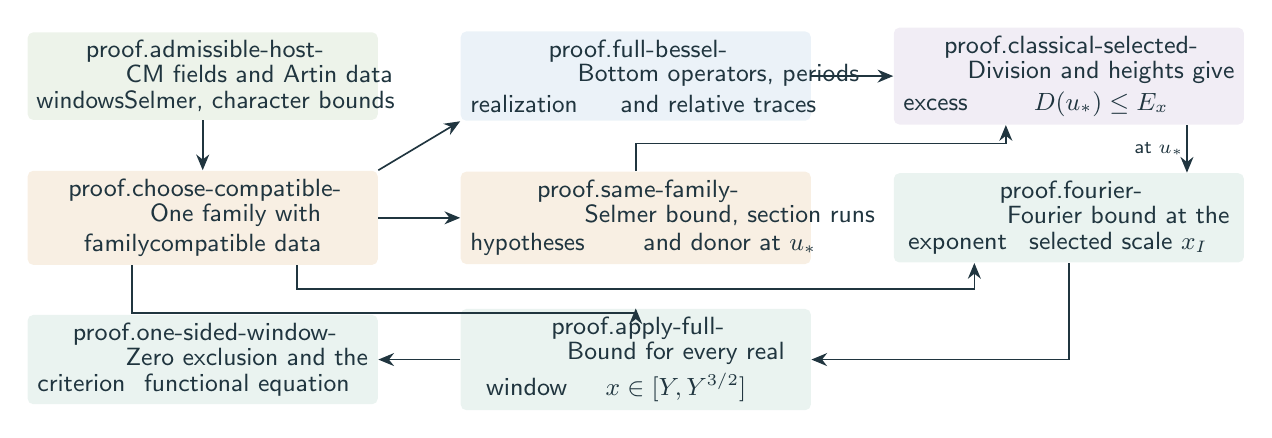
\begin{tikzpicture}[x=1mm,y=1mm]
  \node[argument block,fill=FieldTint] (fields) at (0,0)
    {\hyperlink{proof.admissible-host-windows}{\shortstack{CM fields and Artin data\\Selmer, character bounds}}};
  \node[argument block] (periods) at (55,0)
    {\hyperlink{proof.full-bessel-realization}{\shortstack{Bottom operators, periods\\and relative traces}}};
  \node[argument block,fill=TraceTint] (lattice) at (110,0)
    {\hyperlink{proof.classical-selected-excess}{\shortstack{Division and heights give\\\(D(u_*)\le E_x\)}}};
  \node[argument block,fill=ChoiceTint] (family) at (0,-18)
    {\hyperlink{proof.choose-compatible-family}{\shortstack{One family with\\compatible data}}};
  \node[argument block,fill=ChoiceTint] (inputs) at (55,-18)
    {\hyperlink{proof.same-family-hypotheses}{\shortstack{Selmer bound, section runs\\and donor at \(u_*\)}}};
  \node[argument block,fill=AnalysisTint] (fourier) at (110,-18)
  {\hyperlink{proof.fourier-exponent}{\shortstack{Fourier bound at the\\selected scale \(x_I\)}}};
  \node[argument block,fill=AnalysisTint] (window) at (55,-36)
    {\hyperlink{proof.apply-full-window}{\shortstack{Bound for every real\\\(x\in[Y,Y^{3/2}]\)}}};
  \node[argument block,fill=AnalysisTint] (zeros) at (0,-36)
    {\hyperlink{proof.one-sided-window-criterion}{\shortstack{Zero exclusion and the\\functional equation}}};
  \draw[argument arrow] (periods.east) -- (lattice.west);
  \draw[argument arrow] (fields.south) -- (family.north);
  \draw[argument arrow] (family.north east) -- (periods.south west);
  \draw[argument arrow] (inputs.north) -- ++(0,3.5) -| ([xshift=-8mm]lattice.south);
  \draw[argument arrow] ([xshift=15mm]lattice.south)
    -- node[left,font=\scriptsize\sffamily,text=PageInk,inner sep=1pt] {at \(u_*\)}
       ([xshift=15mm]fourier.north);
  \draw[argument arrow] (family.east) -- (inputs.west);
  \draw[argument arrow] ([xshift=12mm]family.south) -- ++(0,-3)
    -| ([xshift=-12mm]fourier.south);
  \draw[argument arrow] ([xshift=-9mm]family.south) -- ++(0,-6)
    -| (window.north);
  \draw[argument arrow] (fourier.south) |- (window.east);
  \draw[argument arrow] (window.west) -- (zeros.east);
\end{tikzpicture}
\caption[From theta periods to zero exclusion]{The period and trace arguments of
  Sections~\ref{sec:periods}--\ref{sec:trace} share a box.
  Section~\ref{sec:family} supplies Selmer and Artin data for
  Section~\ref{sec:integral} and character estimates for Section~\ref{sec:fourier}.
  The chosen family supplies the word code and the prime level of each word
  for the column-dimension estimates in Section~\ref{sec:trace}.
  The prime powers select a scale \(x_I\) in the admitted interval.
  At its maximizing translate the
  \hyperlink{proof.section-run-family-identification}{selected section runs}
  supply the section comparison and the
  \hyperlink{proof.ramified-donor-identification}{transported donor}
  supplies the column comparison. Apply the lattice implication with
  the other period, rank, trace, gain, height and slope inputs.
  Fourier inversion has two inputs in this schematic. The lattice
  calculation gives the \hyperlink{proof.classical-selected-excess}{one-record
  upper bound}. The host arrays determine the
  \hyperlink{proof.classical-maximizing-translate}{maximizing label} by a finite
  character sum. Both calculations use the same sampling data, cutoff, weights
  and centering. The resulting upper bound at \(x_I\) controls the
  normalized excess on the entire interval.
  The \href{proof-map.html\#window}{window proof map} links these
  implications to their statements and arguments in the paper.}
\label{fig:overview}
\end{figure}


\Needspace{14\baselineskip}
\section*{Candidates for new mathematical results}
\markboth{Candidates for new mathematical results}{}
\addcontentsline{toc}{section}{Candidates for new mathematical results}

We compare the nineteen AI-proposed candidates below with earlier
results under the hypotheses, normalizations and uniformity needed
here. A short deduction from earlier work can supply the required
conclusion. A broader range or a reusable argument can make a
candidate worth recording. The sections specify the scope of the
independent proof checks.

\subsubsection*{Arithmetic windows and Galois cohomology}
\noindent\textbf{\hyperlink{candidate.family}{Uniform bounds for higher fine Selmer groups}}.
Fix the primitive target \(\psi\), \(0<\varepsilon<1/52\) and the
dyadic profile \(h\) from Section~\ref{sec:family}. The release gives
\(J\ge1\) and \(X_0\). For every \(X\ge X_0\) and every pair \(q,d\)
with the prescribed sizes and congruences at \(Z=X^{1/J}\), there is
\(W\ge Z\) with \(W^2\le X\). At every real \(y\in[W,W^2]\), every
CM field \(E\) of the prescribed type at \((h(y),q,d)\) satisfies
\[
 \sum_{\ell\in S}(\log\ell)
   \sum_{1\le r<\lfloor y^{401}\rfloor}s_\ell(E,r)
   \le \exp(y^\varepsilon/2)
 \qquad\text{for every finite set \(S\) of primes}.
\]
Here \(s_\ell(E,r)\) is the length of the localization kernel for the
Tate twist \((-r)\). Duality bounds these lengths at each fixed field
and twist in terms of \(K_{2r}(\mathcal O_E)\)
\cite{f1milne-adt,f1weibel-kbook}. For \(\psi=1\), prime-counting,
zero-density estimates and the explicit formula give the required three
quadratic-twist bounds, their logarithmic-derivative bounds, and the
large-argument estimate for all primitive host associates
\cite{f1thorner-zaman,f1thorner-zaman-density,f1heath-brown,f1ihara-murty-shimura}.
The windows at scale \(x\) give the bound at \(\lfloor x^{400}\rfloor\)
and hence at the realized cutoff \(t\) for the finite-place defect in division.

The \textbf{\hyperlink{candidate.crystalline-rows}{lifting of integral finite
cohomology classes with separated Hodge jumps}} occurs at inert places
in Section~\ref{sec:integral}. Let \(K/\mathbf Q_\ell\) be unramified
of degree \(n\), \(\ell\ge11\), and let \(T_1\twoheadrightarrow T_2\)
be a surjection of crystalline lattices over a coefficient ring
\(\mathcal O\) whose fraction field splits \(K\). Write \(r\) for the
rank of \(T_2\). For each embedding of \(K\), its decreasing-filtration
jumps lie in a central interval and one signed interval. Large
intervals can occur singly or in pairs in Frobenius order, with at
least \(j\) small labels between successive groups. The large
intervals have the prescribed comparable size, separated from the
central interval as in Section~\ref{sec:integral}. Write \(H\) for
the common bound on the absolute endpoints of all the intervals and
\(g\) for the sum of the three small width parameters. For the full
inverse-image Bloch--Kato finite condition the bound is
\[
 \frac{\operatorname{length}_{\mathcal O}
   \operatorname{coker}[H^1_f(K,T_1)\longrightarrow H^1_f(K,T_2)]}
      {\operatorname{length}_{\mathcal O}(\mathcal O/\ell\mathcal O)}
 \ \ll\ (n+1)r\!
 \left(\frac{H}{(\ell-1)^{j+1}}+(g+1)(j+1)+
             \log_\ell\max(1,H)\right).
\]
The cyclic spacing suppresses the contribution from the largest
jumps even when their average width exceeds the Fontaine--Laffaille
range of Zhu's Theorem~B. An integral description of \(H^1_f\) for
an individual lattice with one-sided weights is available from
Čoupek, Gazaki and Marmora \cite{zhu-labelled,cgm-integral}.
In the \hyperlink{proof.crystalline-cluster-lifting}{proof of the
lifting bound}, the intervening small jumps control the loss in
integral Frobenius coordinates. At two large jumps of opposite
signs, compatibility of the two lifts must be proved in both cyclic
orders. The local lifts then give one exponent annihilating the
cokernel, independently of the number of pairs. This supplies the
corresponding inert-place term in the Hecke lattice comparison.

The \textbf{\hyperlink{candidate.residual-crystalline-admissibility}{finite
condition for torsion extensions with prescribed crystalline lifts}}
concerns a fixed lattice. Let \(K/\mathbf Q_\ell\) be unramified,
\(\ell\ge5\), and let the coefficient DVR \(\mathcal O\), with
uniformizer \(\lambda\), contain the integers of every conjugate
of \(K(\mu_\ell)\). Fix a crystalline lattice \(T\) with labelled
filtration jumps \(U_i\), and characters
\(\chi_c=\chi_1\varepsilon_\ell^{1-c}\), \(1\le c\le t\), with
labelled jumps \(w_i+c-1\). Section~\ref{sec:integral} gives
the separation and residue conditions on these jumps at each embedding.
For a finite \(\mathcal O\)-module \(X\) with trivial action, a class
in \(H^1(K,T(\chi_1^{-1})\otimes X)\) gives extensions of
\((\mathcal O/\lambda^a)(\chi_1)\) by \(T\otimes X\) for
\(\lambda^a X=0\). Test whether for every sufficiently large \(a\)
the extension is a quotient of nested stable lattices in a finite
direct sum of crystalline representations. Each summand must have
the full labelled jumps and residual characteristic polynomials of
\((T\otimes\operatorname{Frac}\mathcal O)\oplus\bigoplus_c\chi_c\).
The classes passing the test form exactly the image of
\[
 H_f^1(K,T(\chi_1^{-1}))\otimes_{\mathcal O}X
       \longrightarrow H^1(K,T(\chi_1^{-1})\otimes_{\mathcal O}X).
\]
Here the integral finite group is the inverse image of the rational
Bloch--Kato group. With a lattice in \(\chi_c\) in place of \(T\),
the same test gives zero for \(c\ge2\) and the unramified subgroup
for \(c=1\). In particular, an isomorphism of two crystalline lattices
modulo \(\lambda^a\) identifies their finite images at that precision
when the characters and labelled type agree. This conclusion reaches
some profiles beyond the Fontaine--Laffaille range. For short
crystalline representations over \(\mathbf Q_\ell\), Atobe and
coauthors lift a residue-field subquotient extension together with
suitable endpoints \cite[Lemma~7.6]{atobe-harder-crystalline}.
Here the endpoints are prescribed. The three local conclusions give
zero local loss at the large primes satisfying the separation conditions.

At each of the two type primes a different
\textbf{\hyperlink{candidate.tame-type-lifting}{integral lifting bound}}
uses the Frobenius action on tame inertia characters. Let
\(T_1\twoheadrightarrow T_2\) be a surjection of stable lattices in
potentially crystalline representations of \(G_{\mathbf Q_p}\), over
the integers of a finite extension of \(\mathbf Q_p\). Suppose their
characteristic-zero inertial
types have characters in a common Frobenius-stable set \(\Sigma\)
of at most \(N\) tame characters, including \(1\), with \(N\ge2\).
Their de Rham filtration jumps must lie in a common set of at
most \(N+1\) integers in \([-\eta,H]\) containing zero.
Write \(q\) for the maximum Frobenius orbit length of a ratio
of two characters in \(\Sigma\). If \(1\le\eta<H\) and
\(p>40(HN^2+N^3)\), then
\[
 p^{\,7(Nq+\eta(N+q))}H^1_f(\mathbf Q_p,T_2)
 \ \subseteq\ \operatorname{im}
 \bigl[H^1_f(\mathbf Q_p,T_1)\longrightarrow H^1_f(\mathbf Q_p,T_2)\bigr].
\]
Here the integral finite subgroup is the full inverse image of the
rational Bloch--Kato subgroup. Once the prime satisfies the threshold,
the exponent is independent of the positive endpoint \(H\), the tame
splitting degree and the multiplicities of the characters and jumps.
The covariant Breuil--Kisin comparison gives left exactness and an
unspecified power of \((p,u)\) killing the final module cokernel
\cite[Proposition~3.4]{cgm-integral}. The
\hyperlink{proof.tame-type-lifting}{quantitative argument} first
separates the characters on two ranges of Euler degrees and then
corrects the monodromy of a lifted finite class. At \(g_0,g_1\) the
argument uses \(q\le\lfloor N^2/4\rfloor\) for the graph lattices
of the cohomology maps and their Tate duals. A length bound for
the local Hecke defect also uses the rank of each target.

The \textbf{\hyperlink{candidate.tame-selmer}{integral Selmer bound for tame
anticyclotomic twists}} concerns the finite list of cuspidal lattices
\(T_s\) of odd rank \(r\ge100\) at one stage over the CM field \(E\).
Their conjugate Tate duals are \(T_s\epsilon_\ell^t\), with \(t\)
positive and odd. Here \(\epsilon_\ell\) is the cyclotomic character.
The residual representations are absolutely irreducible. Use the
prescribed Galois representations and finite local conditions of
Section~\ref{sec:integral}, including the Hodge gap, the conditions
on the Tate duals and the common tame inertia element. Put
\(\nu_\ell=\min_{g\in G_E}v_\ell(\epsilon_\ell(g)^{rt}-1)\), with
\(v_\ell(\ell)=1\). Given \(\delta_A,\delta_D>0\) and the prescribed
finite set to avoid, choose one finite \(\ell\)-power anticyclotomic
character \(\psi\), trivial at every decomposition group over
\(\ell\), with tame ramification at split conjugate pairs \(Q\).
For each \(a\) prime to \(\ell\), let \(L_{a,s}\) be the normalized
length of the relaxed finite Selmer group of the twist by
\(\psi^{a\sigma_s}\), with the sign \(\sigma_s\) assigned to \(s\).
The desired conclusions are
\[
  \sum_s (L_{a,s}-\nu_\ell)_+ \le \delta_A
       \quad ((a,\ell)=1),\qquad
  t\sum_{v\in Q}v_\ell(\psi(\tau_v)-1)\le\delta_D ,
\]
where \(\tau_v\) generates the inertia image. On the classical family
\(\nu_\ell=0\) at odd primes and \(\nu_2=1\). The distinction matters
for lengths over ramified coefficient fields. With these hypotheses,
Section~\ref{sec:integral} obtains a bounded-degree coefficient of
valuation at most \(\nu_\ell\) in each integral Selmer determinant
for one choice of split prime pairs. A simultaneous specialization
then gives the common character and both bounds. To pass to the
integral Hecke row, Section~\ref{sec:integral} compares the vacuum
and the algebraic section at the same marked point of every cover.
Their changes of frame cancel, leaving one phase and one harmonic
scalar for the stage. Projecting the finite row vectors to the
quotients by their complementary planes then identifies the
specialized columns in the prescribed twisted lattice. Bounds for
its congruence index also require the local Galois estimates. Earlier
theorems control residual Selmer groups in suitable cyclic twists or
give distributions in specified families of twistable modules
\cite{tame-selmer-mazur-rubin,tame-selmer-smith}. The bound here feeds
the cuspidal contribution to the integral Hecke comparison.

\subsubsection*{Theta and Bessel periods}
At a selected translate with the prescribed unitary towers, real tests,
levels and transport data, the \textbf{\hyperlink{candidate.periods}{theta--Bessel period comparison}}
uses one finite central element and row isometry \(sV\) for all words.
For each \(w\), one unitary \(U_w\) and one \(a_w\ne0\) give, for every
twisting tuple \(\boldsymbol\mu\), ramified column \(\phi\) and projected row \(F_m\),
\[
 b_{w,\boldsymbol\mu}(\phi,F_m)
 =\frac{d_{w,\boldsymbol\mu_0}}{d_{w,\boldsymbol\mu}}\,
 a_w\big\langle sV\iota_{\boldsymbol\mu}F_m,
             \mathcal P_w\jmath_wU_w\phi\big\rangle .
\]
Some positive power of the ratio \(d_{w,\boldsymbol\mu_0}/d_{w,\boldsymbol\mu}\)
is rational and supported on the twisting primes of \(\boldsymbol\mu\).
Seesaw compares matched kernels. The Bessel formula gives normalized
squared periods of factorizable vectors in a fixed tempered representation
with discrete Hermitian weak base change \cite{seesaw,p2bp-chaudouard-bessel}.
The simultaneous comparison permits descent to a common row dual for
the rank argument. The support property preserves valuations at the
finite places where the tuple avoids the residue characteristic.

At a split finite place, the \textbf{\hyperlink{candidate.transfer}{transfer around a square}}
takes an admissible test at depth \(e\ge1\) with the prescribed ramified
unitary determinant ratio of conductor exponent at most \(e\). Partial Fourier transforms and
a primitive-frame integral give the opposite test with integral support,
the same depth and the required level and character actions. In these
Fourier models the large zeta section
equals the complementary small section with the product determinant
character when \(\operatorname{vol}(\mathrm{GL}_a(\mathcal O))=1\).
Related partial transforms construct split doubling sections
\cite{p2eischen-doubling}. The matching lets the calculation of integral
row tests change paths in the grid of lifts.

\textbf{\hyperlink{candidate.fixed-level-period}{Detection at the prescribed principal level}}
is proved in Section~\ref{sec:periods} for the prescribed grids.
Fix the precision and depth constant \(C_F\ge6510\). Beyond one
threshold, take an admissible grid over \(E/F\), its bottom
Hermitian space \(Y\), and \(V=Y\perp\langle1\rangle\).
For every nonzero cuspidal multiplicity map \(t\) on \(U(Y)\) of the
prescribed real type at principal level \((g_0g_1)\), and every
nonzero vector \(w\) in its smooth real tensor space, the assertion
gives a cusp form \(a\) on \(U(V)\) of the prescribed discrete-series
type, with a \(K_\infty\)-finite testing vector, such that
\[
  \int_{[U(Y)]}a(\iota h)t(w)(h)\,dh\ne0 .
\]
The finite level for \(a\) is the principal subgroup for the one
ideal \(\mathfrak m\) specified by the grid before \(t,w\) vary.
Both level characters are trivial. The gain over qualitative
period nonvanishing is uniform control of that level as the field,
rank and real weights vary. For a Hermitian Arthur parameter on
the product group, the global GGP theorem relates a nonzero central
value to a nonzero period on some relevant unitary pair. Harris's
restriction theorem starts with a cuspidal representation of the
larger group with sufficiently regular discrete series at infinity.
Here the smaller row and the larger principal level are both prescribed
\cite{depth-endoscopic-ggp,depth-harris}. The proof bounds a translated
real matrix coefficient relative to its reproducing scalar. At a point
where the row is large, the prescribed depth makes the nonidentity
terms in the Poincar\'e period smaller than the stabilizer term.
Compact averaging then supplies a \(K_\infty\)-finite testing vector.
The \hyperlink{proof.principal-core-span}{spanning argument} expresses
the core tests in terms of descending lifts. The
\hyperlink{proof.principal-fixed-ascent}{ascent argument} transports
the nonzero Bessel pairing along the prescribed core tower.

\subsubsection*{Relative traces and automorphic multiplicities}
The \textbf{\hyperlink{candidate.trace}{mixed Gram estimate}} uses the levels,
real types and rank conditions of the tied family. At each translate the
normalized Poincar\'e operators \(L_w=c_0(w)^{-1/2}\mathcal P_w\) act on full
columns of dimension \(d_w\) and share a Petersson target. With
\(b=\exp(x^\varepsilon)\) and reference dimension \(D_\star\) the estimate is
\[
 \|L_w^*L_v\|_{\rm HS}^2
 \le (1+b^{-6})\,d_wd_v/D_\star
 \qquad(w\ne v).
\]
One threshold works for all selected translates and distinct words.
Relative trace unfolding and density formulas give the orbit reindexing
and primitive counts \cite{tr3getzhahn,tr3hironaka}. The signed scalar main
term and nongeneric corank-one remainder, with absolute bounds on other
errors, control the mixed terms of the second moment for the period span.

The \textbf{\hyperlink{candidate.diagonal}{single-word estimate}} uses the full
columns from the mixed Gram estimate and the balance \(d_w\Gamma^2\asymp D_\star\) of
\eqref{eq:trace-balance}, where \(\Gamma=\exp(C_\Gamma m^5 f\log b)\),
\(f=[F:\mathbb Q]\) and \(k,m\) are the rank parameters. Beyond one
threshold, every selected translate and every word satisfy
\[
 \frac{\|L_w^*L_w-I\|_{\rm HS}^2}{d_w}
 \le 2\exp(-kf\log k)+2C_0/\Gamma.
\]
Schur orthogonality gives the identity term. Bounds on the degenerate and
nondegenerate orbital remainders control the mean-square deviation of the
squared singular values from \(1\). This gives the diagonal trace moments
and, with the ramified column count, a nonzero bottom reference pairing.

The \textbf{\hyperlink{candidate.count}{spectral multiplicity estimate}} fixes a discrete
series at each real place for the unitary group \(G\) of common signature
\((p,q)\) and rank \(r=p+q\), with \(q^2\le r\). Use a finite projector
\(e\) of level \(g\le b^{A}\) with the prescribed split-prime support.
The cross-sign Harish--Chandra gaps must be at least
\(Cr^{19}f^5\log(b\,\operatorname{rd}(E))\).
The projector's rank \(D\) on the multiplicity space satisfies
\(|D-D_\star|\le \exp(-rf\log r/16)D_\star\). The main term \(D_\star\)
is the product of the formal degrees, \(\operatorname{vol}([G])\), and
\(\Re e(1)\). Section~\ref{sec:trace} compares this with multiplicity
theorems for a fixed group and field. The uniform error as \(r,f\) vary
lets the moments measure the span against the actual target dimension.

\subsubsection*{Integral lattices and divisibility}
For the \textbf{\hyperlink{candidate.jet}{short window for perturbed determinant jets}},
let \(v\) be a nonarchimedean valuation on a characteristic-zero field
with \(v(p)=1\), \(p\ge5\) prime. Take \(q=p^h\) for odd \(h\ge1\),
\(\rho=(p^2-1)^{-1}\), \(e=1+(q-p)\rho\) and \(1\le r\le n\).
Let \(X,Y\) be \(r\)-by-\(r\) matrices of independent variables and
\(H\) a formal power series in those variables. With ordinary derivatives set
\[
 \Lambda_y=\left.
   \det(\partial_X)^{qy}\det(\partial_Y)^y
   \exp\!\left(-p^{-e}\sum_{i,j}X_{ij}^{q}Y_{ij}+H(X,Y)\right)
   \right|_{X=Y=0}.
\]
Every nonzero term of \(H\) has positive \(Y\)-degree and coefficient
valuation plus weight at least \(1/(p-1)\). The weights per variable are
\(\rho+3/(8q)\) for \(X\) and \(\rho+1/2-1/(8q)\) for \(Y\).
Every interval of \(\lceil64r^2(h+3+3\log_p(r+1))\rceil\) consecutive
nonnegative integers contains an order \(y\) with
\(v(\Lambda_y)\le ry((q+1)p\rho-1)+n(\log_p n+1)\).
Cayley's identity gives the factorial normalization \cite{lt4cayley}.
The bound for the resulting Newton coefficients makes the short
interval accessible by finite differences. In the local normal form
this supplies a test of controlled valuation for an odd Frobenius block.

The \textbf{\hyperlink{candidate.gain}{realization of Frobenius gains by integral division}}
uses the prescribed Artin data at sufficiently large designated scales, with
sampling degrees, stage weights and metrized period lattices at each
tied translate. Local division realizes valuation gains on the source
lattices enlarged by fractional ideals. The inertia-weighted sum of
ramps \eqref{eq:prime-power-ramp} through \(\lceil2xb\rceil\) is at most
the weighted valuation gain net of restriction plus
\(C_{\rm loss}|T|mbx^{e_L\varepsilon}\), with the same bound for the
weighted index allowance in \eqref{eq:frobenius-gain-loss}.
Height and slope inequalities and the CM period normalization give
the comparison in the prescribed metrics
\cite{tr3chenHN,lt4barquero,siegel-kron}. Combining those inputs with
the realized gains gives the centered inequality \(D(u)\le E_x\) of
\eqref{eq:integral-excess} at every tied translate \(u\). The Fourier
projection uses this inequality with the same sampling data and cutoff.

There is also a \textbf{\hyperlink{candidate.integral-weyl-content}{weightwise
integral refinement}} of the comparison between Weyl and dual Weyl
lattices. Let \(\lambda=(a^t,\kappa)\) be a dominant polynomial
weight, and let \(\Delta,\nabla\) use the same primitive highest
vector. At grade \(i\), take the monic least common multiple
\(D_i(T)\) of the polynomials
\(\prod_{(b,c)\in\tau/\kappa}(T-(c-b))\) over the allowed skew
shapes with nonzero value at \(a\). Each shape has \(i\) boxes,
at most \(t\) in any column, and \(\tau\) has length at most
that of the second block. If \(p^{e_L}\) clears the Levi weight
lattices up to a given depth measured by a decreasing linear
functional, then at every weight \(v\) of grade \(i\) up to
that depth one has
\[
  p^{e_L+v_p(D_i(a))}\nabla(\lambda)_v\subseteq\Delta(\lambda)_v .
\]
Taking the polynomial least common multiple before specializing
retains distinct factors whose values coincide modulo \(p\).
The formula includes singular specializations and primes dividing
\(i!\). Nakahama computed the rational scalar on each isotypic
component \cite[Theorem~1.2]{nakahama-norms}. The candidate is
the resulting denominator on the integral weight lattice, with
the original cutoff on its Levi coefficients. For the bound
summed over primes in this paper, ordinary rational projectors
with a common factorial denominator already suffice. The sharper
statement has a separate application wherever a bound at one
prime and one weight is required. Its historical priority is open.

A local estimate in the height calculation concerns
\textbf{\hyperlink{candidate.mixed-determinant-depth}{divisibility of a
determinant of invariant derivatives}}. Let \(p\) be odd and
\(G\) a commutative formal group over the valuation ring of an
algebraically closed valued field of characteristic zero, with
\(v(p)=1\). For an even integer \(h>0\), suppose
\(\mu_{p^h-1}\) acts integrally with logarithmic types
\(\zeta\mapsto\zeta^{p^s}\), \(s\in\mathbf Z/h\mathbf Z\).
Assume that each odd type has tangent dimension at most \(j\).
Choose any \(i\ge1\) integral tangent vectors in a single even
type whose matrix has a unit \(i\)-minor. Write \(D_a^{(b)}\)
for the invariant derivative along vector \(a\) in copy \(b\)
of \(G^i\). Let \(\delta_c\) be the infimum, over all integral
power series \(f\) on \(G^i\), of
\(v((\det(D_a^{(b)})^c f)(0))\). For every integer \(c\ge1\)
some integer \(0\le r\le\min(i,j(3+\log_p c)/2)\) satisfies
\[
 \delta_c\ \ge\ (i-r)c\,\frac{p}{p^2-1}-i^2(1+\log_p c).
\]
The coefficient \(p/(p^2-1)\) already occurs for a
one-dimensional Lubin--Tate group for the unramified quadratic
extension, with its primitive dual character
\cite[\S V]{depth-katz}\cite[Appendix, Theorem~(c)]{depth-lubin-tate}.
The candidate is the bound on how many directions can lose this
gain in an arbitrary saturated frame of mixed type. The proof
chooses successive bases of \(p\)-typical curves and controls the
dimensions lost at each step. Keeping the separate radius at every
step gives a further consequence in this reconstruction,
\[
 \delta_c\ \ge\ ic\,\frac{p}{p^2-1}
       -jc\,\frac{p^3}{(p^2-1)^2}-i^2\log_p(c+1).
\]
For fixed \(p,i,j\) the loss proportional to \(jc\) in this formula
has a coefficient independent of \(c\). On the arithmetic family
a bounded number of steps already suffices at the small inert primes.
This estimate concerns every integral germ. The separate bound for perturbed
determinant jets selects a term in the jet.

The \textbf{\hyperlink{candidate.marked-frobenius-pairing}{Frobenius pairing on
two prescribed tangent planes}} occurs before the estimate for perturbed determinant jets is applied.
Take a prime \(p\ge5\) in either alternating case of the local
index calculation and its polarized Raynaud extension with unramified CM action.
On each of two paired Frobenius cycles the tangent ranks alternate
between \(n+j\) and \(j'\). In the self-conjugate case use two
copies of the factor as in Section~\ref{sec:integral}.
Fix an odd \(0<i<D\), where \(D\) is the full cycle length.
Prescribe integral rank-\(n\) direct summands in the large types
\(a\) and \(\overline{a+i}\) on opposite sides. Put \(q=p^i\) and
\(E_i=1+(q-p)/(p^2-1)\). There are saturated subplanes of equal
rank \(s\ge\max(0,n-ij'-j)\) inside these summands such that the
mixed coefficient of the polarized biextension, in formal
logarithm coordinates on them, satisfies
\[
 p^{E_i}[Gh]_{q,1}\bmod\mathfrak m
      =-\sum_{b=1}^s x_b^q y_b
\]
in suitable integral bases. Here \(h\) is its rigidified additive
gauge, \(G\) is the unit scalar of the level, and \(\mathfrak m\)
is the maximal ideal in the valuation ring of the completed
algebraic closure at \(p\), with \(v(p)=1\).
The coefficient thus gives a perfect pairing after Frobenius
twist. The proof bounds the other coefficients on the same
planes, which allows the determinant estimate to be applied.
Classical display theory constructs the biextension from the
polarization \cite[\S4.3]{cartier-display}. The candidate concerns
the uniform rank and the separation of this coefficient when
both tangent planes are prescribed.

\subsubsection*{Heights, section lattices and Fourier--Jacobi coefficients}
The \textbf{\hyperlink{candidate.height}{finite-degree bound for metrized
adjoint section lattices}} gives, for a birational moving system of degree
\(d_Z\) on a flag component of dimension \(s\), a degree lower bound
with leading term
\(\binom{\ell-1}{s}d_Z\,\ell h_Z\), with normalized Chow height \(h_Z\) and
the chosen degree \(\ell\ge3s+5\). It uses controlled multiplication,
short integral frames and rank and metric comparisons. The Chow determinant
method has precedents in David--Philippon and Chen. The chosen degree may
lie below a projective Hilbert-point threshold. After descent from the
cover and truncation, the component bounds control the covolumes of
cusp-section lattices in the indefinite tower. These covolumes enter
the division estimates. The reference slopes on the definite column
spaces require a separate calculation.

The \textbf{\hyperlink{candidate.flag-height}{height of the metrized full flag
at finite cutoff}} enters the mean slope on a nonterminal unitary cover.
Let the abelian CM field \(E\) have degree \(2f\), \(f\ge2\), and take
the CM type induced from the specified imaginary quadratic field.
Each label has signature \((p,q)\), with \(q\ge1\) and \(N=p+q\ge3q+1\).
Use the prescribed good level \(M'\) with auxiliary parameter \(A=1\)
and at most \(4fN^2\) exceptional prime divisors of
\(2|\operatorname{disc}E|M'\). The compatible integral models are
chosen before the weight and cutoff. For a strictly decreasing weight
\(u\), require that, at each label, every one of the last \(q\) entries
be at distance at least \(g>0\) from each other entry. Take an integer
\(B\) with \(B+1>4fN^2(1+\|u\|_\infty/g)\). The integral Hodge--Tate
lattices are used at the exceptional primes and at all primes up to \(B\).

Put \(D=f\binom N2\). Let \(H_B(u)\) be the sum of the normalized
arithmetic self-intersections of the metrized weight line on the
components, divided by \(D+1\) times the sum of their geometric
degrees. With the prescribed quadratic character \(\chi_{d_0}\) set
\(\Lambda_B=\log(B\,\operatorname{rd}E)+|\Re(L'/L)(1,\chi_{d_0})|\).
Section~\ref{sec:integral} obtains the absolute lower bound
\[
 H_B(u)\ \ge\ -C\left(\Lambda_B\sum_{\tau,i}|u_{\tau i}|
              +q\sum_\tau(\max_i u_{\tau i}-\min_i u_{\tau i})\right).
\]
This controls a height used to estimate the mean of the component Chow
heights in the finite-degree adjoint bound. Geometric proportionality
gives the ordinary flag degrees \cite{flag-hormann}. Arithmetic volume
formulas for a Hodge line in signature \((n-1,1)\) over an imaginary
quadratic field, or with only one noncompact real place, concern fixed
integral models \cite{flag-bruinier-howard,flag-guo}. The equivariant
arithmetic Chern character formulas for abelian schemes in
\cite{flag-maillot-rossler} apply away from the coefficient discriminant.
Here each newly selected good prime changes the integral flag.
Section~\ref{sec:integral} computes that change on the common finite
model, including its toroidal boundary, and bounds the resulting
prime tail. On each fixed cover the mixed intersections converge to
those for the prescribed Hodge metric. The proof tests weights on the
walls of the dominant chamber with positive last entry at each real
place. Polynomial continuation then includes the signed weights that
occur in the estimate. Two determinant heights account for the terms
that survive the wall tests. This gives the displayed component mean
at the original cutoff. Applying it to a lattice of sections also
uses the finite-place trace and the norms of sections on that cover.

The \textbf{\hyperlink{candidate.cm-boundary-fourier-jacobi}{detection of a
prescribed Fourier--Jacobi coefficient at a CM boundary}} concerns
either principal-level cover at a nonterminal stage. Fix an isotropic
line of the marked unitary lattice and a frequency \(\nu\) with
\(0<\sum_{\tau}\nu_\tau\le c_1\), where the sum is over the \(f\)
embeddings in the CM type.
If this coefficient of a complex cusp section is nonzero, there is
a one-parameter degeneration with CM abelian part and torsion
extension data on which a Laurent coefficient, followed by a monomial
coefficient in the tangent frames, detects it. The resulting linear
functional kills every section whose coefficient at this line and
frequency vanishes. Let \(E\) be the CM field of degree \(2f\),
\(r\) the unitary rank, \(M\) the level, \(d_E=|\operatorname{disc}E|\),
\(N_A,N_c\) the two lattice comparison integers, and
\(W\) the bound for the analytic weight spread. If \(X\ge1\) bounds
\(f,r\) and the logarithms of \(M,d_E,N_A,N_c,c_1,W\), the torsion
denominator \(n_Q\) and the factor \(\Lambda_Q\) bounding the lengths
of the CM tangent generators satisfy
\[
       \max(\log n_Q,\log\Lambda_Q)\le 200X^2 .
\]
The same functional has bounded denominators at every finite place
and bounded operator norm at every complex embedding, in its
metrized value line. It therefore gives a lower bound for the
first minimum of the integral quotient by sections whose low
coefficients all vanish. The proof begins at a point where the
prescribed coefficient is large. Positivity of the rank-two Fourier
indices bounds the reduced lattice minimum there, allowing the
sign plane and the extension data to be varied together.
Pasten uses Heegner points to bound norms of integral differentials
on quaternionic Shimura curves \cite[\S\S13--14]{pasten-cm-norm}.
Richter and Westerholt-Raum use specialization of Jacobi forms at
torsion points for Siegel modular forms modulo a prime
\cite[proof of Proposition~2.4]{richter-westerholt-sturm}. Here the
uniform bounds on a test for the specified boundary coefficient enter
both the rational rank and the integral height of the quotient.

\section{CM fields with character and Selmer bounds}
\label{sec:family}

Fix a primitive Dirichlet character \(\psi\) of conductor \(M\) and a
real exponent parameter \(0<\varepsilon<1/52\). The zeta case takes
\(\psi=1\) of conductor \(1\). For every nonprincipal Dirichlet
character \(\chi\), \(L(s,\chi)\) is holomorphic at \(s=1\) and
\(L(1,\chi)\ne0\) \cite[\S25.15(i) and (25.15.9)]{dlmf}. For
primitive nonprincipal \(\chi\) define
\begin{equation}
\label{eq:centred-prime-sums}
  G_\chi(y)=\sum_{n\ge1}\Lambda(n)\chi(n)(y/n-1)_+
                  +y\frac{L'(1,\chi)}{L(1,\chi)}
  \qquad(y>0).
\end{equation}
For \(\chi=1\), use the zeta sum \(G_1\) of \eqref{eq:principal-ramp}.

At each real scale \(x\), the local division estimates require bounds
on Selmer groups over a CM field \(E\). The Fourier estimate requires
prime-sum bounds for characters of \(\operatorname{Gal}(E/\mathbf Q)\).
The two bounds hold for the same choice of \(E\) at each point
of the intervals used to construct the family. The classical
lattice and Fourier comparison will evaluate that family at
\hyperlink{proof.classical-window-test-scale}{one scale in each window}.

\subsection{The auxiliary primes and character estimates}

At an auxiliary scale \(Z\), put \(w=Z^{\varepsilon/5}\). The primes
\(q,d\) are distinct and coprime to \(M\), with
\[
\begin{gathered}
 q\equiv3\pmod 8,\qquad d\equiv7\pmod {16},\qquad
 q\mid d+1,\qquad p\mid d+1\quad(3\le p\le w,\ p\text{ prime}),\\
 \tfrac12w<\log q\le w,\qquad
 \tfrac12w(\log Z)^2<\log d\le w(\log Z)^2 .
\end{gathered}
\]
Write \(\eta_q=(\frac{\cdot}{q})\) and \(\eta_d=(\frac{\cdot}{d})\) for
the quadratic Dirichlet characters. For \(h\ge0\) let
\[
 E(h,q,d)=\mathbf Q(\zeta_{2^{h+2}})^+\,\mathbf Q(\psi)\,
              \mathbf Q(\sqrt{-q},\sqrt{-d}),
\]
where \(\mathbf Q(\psi)\) is the subfield of \(\mathbf Q(\zeta_M)\)
fixed by the kernel of \(\psi\). Since \(E(h,q,d)\) is abelian and
contains \(\mathbf Q(\sqrt{-q})\), it is CM.

For an odd or \(4\)-divisible modulus \(N\), the cyclotomic Artin map
identifies \((\mathbf Z/N\mathbf Z)^\times\) with
\(\operatorname{Gal}(\mathbf Q(\zeta_N)/\mathbf Q)\) by
\(a\mapsto(\zeta_N\mapsto\zeta_N^a)\). At any prime \(\ell\nmid N\)
the residue class of \(\ell\) gives the arithmetic Frobenius.
For a prime \(p\equiv3\bmod4\), the unique quadratic subfield of
\(\mathbf Q(\zeta_p)\) is \(\mathbf Q(\sqrt{-p})\), and the
restriction of the automorphism indexed by \(a\bmod p\) to it acts
on \(\sqrt{-p}\) by the sign \((\frac ap)\).
\cite[Ch.~V, Examples~3.1--3.2 and 3.11]{f1milne-cft}
Applying this to \(q,d\) gives the quadratic factors of conductors
\(q,d\). These are coprime to \(\operatorname{lcm}(2^{h+2},M)\) and to
each other, so the Chinese remainder theorem gives
\(\Gamma=\operatorname{Gal}(E(h,q,d)/\mathbf Q)\simeq
(\mathbf Z/2\mathbf Z)^2\times H\), with \(H\) the group of the
compositum of the first two factors.
For \(a\) coprime to \(2Mqd\), let \(h_{\rm nat}(a)\in H\) be the
restriction of the cyclotomic automorphism \(\zeta\mapsto\zeta^a\)
to the compositum. Put \(h_-=h_{\rm nat}(-1)\), so \(2h_-=0\).
Write \(\eta_d(a)=(-1)^{e_d(a)}\) and \(\eta_q(a)=(-1)^{e_q(a)}\).
The release's
\releasecite{Formalism/SharpRestriction/RamificationFrobenius/TotientGaloisClasses/InertiaGaloisSymmetry/AnyFrame.lean}{235}{Artin map}
orders the signs as \(q,d\) and shifts the last component to
\(h_{\rm nat}(a)+e_q(a)h_-\). The
\releasecite{Development/AutomorphicArithmetic/PrimitiveCosets/RecH.lean}{10}{Fourier coordinates}
interchange the two sign positions, giving
\begin{equation}
\label{eq:artin-coordinates}
 \operatorname{Art}(a)
 =\bigl(e_d(a),e_q(a),h_{\rm nat}(a)+e_q(a)h_-\bigr).
\end{equation}
Both sign bits of \(-1\) are \(1\), so complex conjugation has
coordinates \(c_\infty=(1,1,0)\). For \(\psi=1\) the compositum is
totally real and \(h_-=0\).

For odd primes \(\ell\nmid d\), splitting in \(\mathbf Q(\sqrt{-d})\)
is equivalent to \(-d\) being a square modulo \(\ell\). For \(\ell=2\)
it is equivalent to \(-d\equiv1\pmod8\), since \(-d\) is an odd
quadratic discriminant. Thus \(2\) and the specified odd primes
dividing \(d+1\) split. These include \(q\) and, once \(w\ge4M\),
every odd prime dividing \(M\).

\paragraph{The classical host and its Artin data.}
For \(\psi=1\), put \(Q_S=2^{h+2}\) and \(Q=Q_Sqd\). The field
\(E=E(h,q,d)\) is the fixed field in \(\mathbf Q(\zeta_Q)\) of the
units \(a\) satisfying \(a\equiv\pm1\bmod Q_S\) and
\(\eta_q(a)=\eta_d(a)=1\). Indeed, these are precisely the
automorphisms fixing each of its three factors. This also identifies
any field of the prescribed type in the Selmer assertion with \(E\).
In an ambient cyclotomic field of a multiple of \(Q\), its defining
subgroup is the inverse image of the same subgroup modulo \(Q\).
The group \(H=(\mathbf Z/Q_S\mathbf Z)^\times/\{\pm1\}\) has order
\(2^h\) and is cyclic. The class of \(5\) generates it, since
\(v_2(5^{2^j}-1)=j+2\) by repeated squaring and no power of \(5\)
is \(-1\bmod 4\). Here \(H=H_0\). The fixed field \(F=E^{\langle
c_\infty\rangle}\) is totally real and \([F:\mathbf Q]=2|H|\).

For \(p\mid Q\), the \(p\)-power cyclotomic factor is totally ramified
locally, by the Eisenstein polynomial of \(\zeta_{p^a}-1\) when
\(p^a\Vert Q\). The roots of unity of order prime to \(p\) lie in the
maximal unramified extension, by lifting the roots in the residue
field. Arithmetic Frobenius raises these roots to their \(p\)-th
powers. Thus the inertia subgroup is the image of the \(p\)-factor
of the group of units in the Chinese-remainder decomposition. In
the coordinates of \eqref{eq:artin-coordinates} this gives
\begin{equation}
\label{eq:classical-host-inertia}
 I_2=\{(0,0,s):s\in H\},\qquad
 I_q=\{0,(0,1,0)\},\qquad I_d=\{0,(1,0,0)\},
 \qquad I_p=\{0\}\quad(p\nmid Q).
\end{equation}
None of these contains \(c_\infty=(1,1,0)\), so \(E/F\) is
unramified at all finite places. Put \(c(e_d,e_q,s)=(-1)^{e_d}\)
and \(P=\ker c\). Both \(2\) and \(q\) split in
\(\mathbf Q(\sqrt{-d})\). Therefore every Frobenius lift at \(2\)
or \(q\), as well as its inertia subgroup, lies in \(P\).
For every lift \(F_d\) and every integer \(j\ge1\), the coset
\(jF_d+I_d\) has one element outside \(P\), since \(c\) is
nontrivial on \(I_d\). At \(p\nmid Q\) the Frobenius is
\(\operatorname{Art}(p)\). These assertions give the local inputs
to \eqref{eq:prime-power-ramp} and its Fourier expansion. The character
\(c\) induces the primitive character \(\eta_d\).

\teamanchor{proof.classical-host-roots-of-unity}%
For large scales \(q,d>3\), the roots of unity in \(E\) are
\(\{1,-1\}\). If an odd prime \(\ell\) divides the order of a
root of unity in \(E\), then \(\mathbf Q(\zeta_\ell)\subset E\).
Its ramification at \(\ell\) forces \(\ell=q\) or \(d\), by
\eqref{eq:classical-host-inertia}. Its inertia order \(\ell-1\)
would then divide \(2\), which is impossible. The unit class equal
to \(-1\bmod Q_S\) and \(1\bmod qd\) fixes \(E\) in
\(\mathbf Q(\zeta_Q)\) and acts nontrivially on \(\zeta_4\).
Thus \(E\) contains no root of unity of order divisible by \(4\).

For \(h\ge1\) there is just one nontrivial real character \(\nu\)
of \(H\). On odd integers it is \((2/\cdot)\), since the class of
\(5\) has value \(-1\) and the map through units modulo \(8\) is even.
Its primitive conductor is \(8\); for \(h=0\) there is no such \(\nu\).
Consequently the real primitive host associates are precisely
\(\rho\eta_q^i\eta_d^j\), with \(\rho=1\) or \(\nu\) when available
and \(i,j\in\{0,1\}\). Their conductors are
\(\operatorname{cond}(\rho)q^id^j\). The same product of conductors
holds if \(\rho\) is any primitive character induced by a character
of \(H\), since the three prime-power parts of \(Q\) are coprime.

For the two prime counts, use Thorner and Zaman's exceptional-zero
convention. For \(m\ge2\) the product of Dirichlet \(L\)-functions
modulo \(m\) has no zero in
\[
 \Re s\ge 1-\frac{1}{13\log(m(|\Im s|+3))}
\]
apart from a possible simple real zero \(\beta_m\) of a unique real
nonprincipal character \(\chi_m\bmod m\). If this zero exists, then
\(1-\beta_m\ge b_0 m^{-1/2}\) for an effective absolute \(b_0>0\).
\cite[arXiv v2, preceding Theorem~1.1 and (1.2)]{f1thorner-zaman}

For real \(U\ge8\) and \((a,m)=1\), let \(\lambda=1\) if there is
no exceptional zero. If there is one, let \(\lambda\) be the mean of
\(1-\chi_m(a)t^{\beta_m-1}\) on \((U/2,U]\), so that
\begin{equation}
\label{eq:family-prime-multiplier}
 \tfrac18\min\{1,(1-\beta_m)\log U\}<\lambda<2.
\end{equation}
Put \(\theta=32/37\) if the exceptional zero exists and \(7/12\)
otherwise. If \(\lambda U/(2\varphi(m))\ge U^{\theta+1/100}\), the
half-interval case of the relative prime number theorem is
\[
 \sum_{\substack{U/2<p\le U\\ p\equiv a\bmod m}}\log p
 =\frac{\lambda U}{2\varphi(m)}
 \left(1+O\left(\exp\left(
   -\frac{c\log U}{\log m+(\log U)^{2/5}(\log\log U)^{1/5}}
 \right)\right)\right).
\]
The constant \(c>0\) and the implied constant are effective and
uniform in \(U,m,a\).
\cite[arXiv v2, Theorem~1.1 and (1.7)]{f1thorner-zaman}

Use \((U/2,U]\subset(\sqrt U,U]\) for both candidate counts. For \(q\)
take \(m_0=8\), \(a=3\) and \(U=e^w\). These candidates satisfy \(q>w\)
for large \(Z\). With \(q\) fixed, the Chinese remainder theorem makes
the congruences for \(d\) a reduced class modulo
\[
  m_0=16q\prod_{\substack{3\le p\le w\\ p\ {\rm prime}}}p,
  \qquad U=\exp\bigl(w(\log Z)^2\bigr).
\]
For any real \(v>0\), Rosser and Schoenfeld give
\(\sum_{p\le v}\log p<1.01624v\)
\cite[Theorem~9, (3.32)]{rosser-schoenfeld}. At \(v=w\) this gives
\(\log m_0\le4\log U/(\log Z)^2\) for both candidate counts when \(Z\)
is large. Both choices also have \(\log U\ge Z^{\varepsilon/6}\).
The bounds on \(\beta_{m_0}\) and \(\lambda\) give
\(\lambda\gg m_0^{-1/2}\). Thus the main term is
\(\gg U m_0^{-3/2}=U^{1-o(1)}\), meeting the condition
\(U^{\theta+1/100}\) since \(\theta\le32/37\). The relative error
is \(o(1)\) uniformly in these moduli. Dividing by \(\log U\)
gives at least \(U^{1-o(1)}\) candidates, uniformly in the first
prime when choosing the second.

\Needspace{10\baselineskip}
\teamanchor{proof.auxiliary-primes}%
For each fixed \(J\ge1\) and all sufficiently large \(Z\), we need one
pair as above satisfying both assertions below. The classical proof for
\(M=1\) follows. For fixed \(M>1\), Alp\"oge's
\releasecite{Development/AutomorphicArithmetic/MeanSquareBounds/pairEx.lean}{112}{theorem on simultaneous quadratic twists}
supplies such a pair.

\begin{enumerate}
\item\label{item:centred-twists} For every character \(\xi\) modulo \(M\) and
  \((i,j)\in\{0,1\}^2\setminus\{(0,0)\}\), let \(\chi\) be the
  primitive character agreeing with \(\xi\eta_q^i\eta_d^j\) on the
  positive integers coprime to \(2Mqd\). For every real \(y\in[Z,Z^J]\),
  \[
    |G_\chi(y)|\le y^{1/2+\varepsilon/2}.
  \]
\item\label{item:twist-boxes} For every real primitive character \(\rho\) of conductor
  dividing \(8M\) and the same pairs \((i,j)\), the primitive
  character agreeing with \(\rho\eta_q^i\eta_d^j\) on those integers
  has no zero in
  \[
    \Re s>1-1/400,\qquad
    |\Im s|\le8M\exp\bigl(w+jw(\log Z)^2\bigr).
  \]
\end{enumerate}

Choose \(q\) first and then test twists by \(\eta_d\) in the progression
it determines. For any real \(R\ge3\),
Thorner and Zaman's density theorem gives
\[
 \sum_{f\le R}\ \sum_{\substack{\chi\bmod f\\ \chi\ \mathrm{primitive}}}
 \#\{\varrho:L(\varrho,\chi)=0,\ \Re\varrho>399/400,\
                              |\Im\varrho|\le R\}
 \le C R^{99/400}
\]
with an absolute effective \(C\). The count uses multiplicities and
includes real exceptional zeros.
\cite[arXiv v4, (1.1)--(1.2) and Theorem~1.2]{f1thorner-zaman-density}
In item~\ref{item:twist-boxes}, the two stages use \(R=8MU\) for \(q\)
and \(R=8Me^wU\) for \(d\). A failing twist has conductor divisible by
the candidate prime, with remaining factor at most \(8M\) or \(8Mq\),
respectively. That factor is smaller than every candidate at its
stage. Thus distinct rejected primes give distinct primitive
characters. Since \(R=U^{1+o(1)}\), these exclusions remove
\(o(U^{9/10})\) candidates.
For the general fixed target, the
\releasecite{Development/AutomorphicArithmetic/MeanSquareBounds/StagePow.lean}{41}{mean-square argument}
assumes every prime factor of the progression modulus is at most
\(w\) or greater than \(Z^{400J}\). The former holds for every factor of
\(8\) and for the small primes in the second modulus. Its other factor
\(q\) satisfies \(q>e^{w/2}>Z^{400J}\) for sufficiently large \(Z\).
The release controls the maximum on each dyadic block by a second
moment bound and uses it to choose one pair meeting both conditions.

For the characters in item~\ref{item:centred-twists}, evaluation at \(Z\) also gives
\[
 \left|\frac{L'(1,\chi)}{L(1,\chi)}\right|
 \le 1+ \frac{1}{Z}\sum_{n\le Z}\Lambda(n)\lfloor Z/n\rfloor
 =1+\frac{\log(\lfloor Z\rfloor!)}{Z}
 \le4\log y\qquad (y\ge Z).
\]

\paragraph{The zeta case from classical prime estimates.}
Fix \(J\ge1\), put \(\sigma=\tfrac12+\varepsilon/8\) and
\(T_0=Z^{2J}\).
\teamanchor{proof.real-character-zero-density}%
For \(Q_0,T_0\ge2\) and \(1/2\le\sigma<1\),
Heath-Brown's real-character density bound is
\[
 \sum_{\substack{\chi\ \mathrm{real,\ primitive}\\
                  \operatorname{cond}(\chi)\le Q_0}}
 N(\sigma,T_0,\chi)
 \ll_\alpha (Q_0T_0)^\alpha
      Q_0^{3(1-\sigma)/(2-\sigma)}T_0^{(3-2\sigma)/(2-\sigma)}
 \qquad(\alpha>0),
\]
where \(N(\sigma,T_0,\chi)\) counts zeros, with multiplicity, in
\(\sigma\le\Re s\le1\), \(|\Im s|\le T_0\)
\cite[Corollary~1 and Theorem~3]{f1heath-brown}.
For the first prime, take \(Q_0=U=e^w\) and test \(\eta_q\).
For the second, take \(U=\exp(w(\log Z)^2)\), \(Q_0=qU\) and test
\(\eta_d\) and \(\eta_q\eta_d\). The two single-prime characters are
odd and their product is even. Their conductors are \(q,d,qd\),
respectively, so each test assigns distinct real primitive
nonprincipal characters to distinct candidates at its stage.
In each stage \(Q_0=U^{1+o(1)}\) and \(T_0=U^{o(1)}\).
The conductor exponent is \(1-\delta\) for
\(\delta=(2\sigma-1)/(2-\sigma)>0\). Taking \(0<\alpha<\delta/4\)
excludes \(O(U^{1-\delta/2})\) candidates in each stage.
Intersect with the tall-rectangle exclusions above at \(M=1\).
They test \(\rho\eta_q\) first, and \(\rho\eta_d,\rho\eta_q\eta_d\)
second, for all real primitive \(\rho\) of conductor dividing \(8\).
Each failing character at a stage contains its candidate prime
in its conductor. The bounds \(O(U^{1-\delta/2})\) and
\(O(U^{99/400+o(1)})\) each exclude a proportion \(o(1)\) of the
\(U^{1-o(1)}\) candidates already counted in the progression.
We may choose \(q\) first and then \(d\) from the surviving primes,
with the second-stage bounds uniform in \(q\). This proves
item~\ref{item:twist-boxes} and leaves each of the three tested
characters without a zero in the Heath-Brown rectangle.

For a primitive nonprincipal character \(\chi\) of conductor \(f\),
let \(D_\chi=L'(1,\chi)/L(1,\chi)\) and
\(A_\chi(y)=\sum_{n\le y}\Lambda(n)\chi(n)(y/n-1)\).
The explicit formula over \(\mathbf Q\) gives, for real \(y\ge2\),
\[
 A_\chi(y)+(y-1)D_\chi
  =\sum_{\varrho}\frac{y^\varrho-1}{\varrho(1-\varrho)}
    +\frac{y-1}{2}\begin{cases}
         F_1(y), & \chi(-1)=1,\\
         F_3(y), & \chi(-1)=-1 .
       \end{cases}
\]
Here the zeros are the nontrivial zeros counted with multiplicity,
initially with a symmetric cutoff in height. The functions in the
formula are
\[
\begin{aligned}
 F_1(y)&=\log\frac{y+1}{y-1}
                +\frac{2}{y-1}\log\frac{y+1}{2},\\
 F_3(y)&=\log\frac{y^2}{y^2-1}
                +\frac{2}{y-1}\log\frac{2y}{y+1}.
\end{aligned}
\]
Indeed, at \(K=\mathbf Q\) the smoothed prime sum in the source
is \(A_\chi(y)/(y-1)\), and its constant for a nonprincipal
character is \(D_\chi\). The two archimedean choices follow from the
action on the real place. For \(y\ge2\) both archimedean terms are
\(O(\log(2y))\) with an absolute constant.
\cite[\S2.1 and Theorem~1, (2.2.1), pp.~256--257]{f1ihara-murty-shimura}
By the functional equation, the three selected real characters
have \(1-\sigma<\Re\varrho<\sigma\) for \(|\Im\varrho|\le T_0\)
\cite[(25.15.5)]{dlmf}.
Let \(N_\chi(t)\) count zeros with \(0<\Re\varrho<1\) and
\(|\Im\varrho|\le t\), including multiplicities. For a character
of conductor \(f>1\) and \(t\ge5/7\), Bennett--Martin--O'Bryant--Rechnitzer
give
\[
 \left|N_\chi(t)-\frac{t}{\pi}\log\frac{ft}{2\pi e}\right|
 \le \min\{0.247\log(ft)+6.894,\ 0.298\log(ft)+4.358\}.
\]
Apply this to the three primitive characters of conductors \(q,d,qd\).
\cite[Corollary~1.2, p.~1456]{f1bennett-zeros}
Thus the number of zeros in
\(n\le|\Im\varrho|<n+1\) is \(O(\log(f(n+3)))\). Use
\(N_\chi(n+1)-N_\chi(n-1)\) for \(n\ge2\), and \(N_\chi(2)\)
for \(n=0,1\).
For \(|\Im\varrho|\le T_0\) the reciprocal denominator is
\(O_\varepsilon((1+|\Im\varrho|^2)^{-1})\).
For \(|\Im\varrho|>T_0\) use \(|y^\varrho-1|\le2y\) and the
reciprocal bound \(|\Im\varrho|^{-2}\). Summing over the unit-height
strips gives an absolutely convergent zero sum and the bound
\[
 |A_\chi(y)+(y-1)D_\chi|
 \ll_\varepsilon y^\sigma\log(3f)
          +\frac{y}{T_0}\log(3fT_0)+\log(2y).
\]
The conductor and height satisfy
\(\log(3fT_0)\ll_J Z^{\varepsilon/5}(\log Z)^2\). For every
\(y\in[Z,Z^J]\) this gives
\[
 y^\sigma\log(3f)\ll_J y^{1/2+13\varepsilon/40}(\log y)^2,\qquad
  \frac{y}{T_0}\log(3fT_0)\ll_J Z^{-J+\varepsilon/5}(\log Z)^2.
\]
At \(y=Z\), use \(|A_\chi(Z)|\le\log(\lfloor Z\rfloor!)\) and
divide by \(Z-1\) to get \(|D_\chi|\le4\log Z\) for large \(Z\).
Adding \(D_\chi\) gives the centering in \eqref{eq:centred-prime-sums}.
Since \(13/40<1/2\), this proves
\(|G_\chi(y)|\le y^{1/2+\varepsilon/2}\) for all real
\(y\in[Z,Z^J]\) with the same pair, proving
item~\ref{item:centred-twists} for \(M=1\). For general \(M\), the twisted
characters in item~\ref{item:centred-twists} can be complex and
the release's prime-pair argument applies to those characters.

\paragraph{Mean squares in the two progressions.}
Let \(P=\{p:\sqrt U<p\le U,\ p\equiv a\bmod m_0\}\) be the
prime set at either stage above. For \(L=Z^A\), \(A\ge J\) fixed,
\(|\kappa(n)|\le1\) independent of \(p\), and \(y\in[Z,Z^J]\), set
\[
 S_L(y,p;\kappa)=\sum_{n\le L}\Lambda(n)\min(1,y/n)\kappa(n)
                         \Bigl(\frac np\Bigr).
\]
Then \(\sum_{p\in P}|S_L(y,p;\kappa)|^2\ll |P|y\log y\) with an
absolute constant for sufficiently large \(Z\).
For the relative factor \(|P|\), use the full-interval prime theorem
modulo \(m_0s\) at \(t\in[\sqrt U,U]\), for odd squarefree
\(1<s\le L^2\) coprime to \(m_0\).
Here \(\log(m_0L^2)\ll\log U/(\log Z)^2\), so
\(t\ge(m_0s)^{12}\) and the relative error is
\(O(\exp(-c(\log Z)^2))\) for some \(c>0\).
Summing over the reduced classes above \(a\) with weights
\((\frac{\cdot}{s})\) cancels the principal term. The secondary
term survives only if the exceptional character restricts to
\((\frac{\cdot}{s})\) on \((\mathbf Z/s\mathbf Z)^\times\).
The relative error is bounded using the sum of the nonnegative
main terms over those classes, including a possible bias from
a character induced from \(m_0\)
\cite[arXiv v2, Corollary~1.4 and Remark~1.5]{f1thorner-zaman}.
In the matching case the secondary term sums to zero without
the weights. Its signed contribution is negligible if
\(1-\beta\ge c/\log(m_0L^2)\), for fixed \(c>0\).
For \(Q_0>100\), the Landau--Page theorem gives an absolute
\(c_{\rm LP}>0\) such that among primitive characters of conductor
at most \(Q_0\), at most one character can have a real zero
\(\beta>1-c_{\rm LP}/\log Q_0\). An exceptional character is
quadratic \cite[Landau--Page; the real-axis case of Lemma~7.1 in the cited account]{f1page}.
Take \(Q_0=m_0L^2\) and \(c\le c_{\rm LP}\).
Since \(s\) is coprime to \(m_0\), the primitive quadratic
character of modulus \(s\) has conductor \(s\). In the matching
case the part of the exceptional conductor supported outside
\(m_0\) is therefore exactly \(s\). A single exceptional
character can affect at most one such \(s\).
Partial summation therefore gives
\(\sum_{p\in P}(\frac ps)=O_B(|P|Z^{-B})\) for every fixed \(B>0\),
with at most one exceptional \(s>1\).

Chebyshev's bound and partial summation make the contribution to
\(S_L\) from proper prime powers \(O(\sqrt y)\). Primes dividing
\(m_0\) contribute \(O(\log m_0)\).
For the remaining primes \(r\le L\), the weights
\(b_r=(\log r)\min(1,y/r)\) satisfy \(\sum_r b_r^2\ll y\log y\),
\(\max_r b_r\le\log y\) and \(\sum_r b_r\ll y(1+\log L)\).
Quadratic reciprocity on the fixed class modulo \(4\) reduces
the distinct-prime correlations to the last character average
with \(s\) the product of the two primes. At most one unordered
pair is exceptional. Its weight is \(O((\log y)^2)\), and the
other correlations contribute \(O_B(|P| Z^{-B} y^2(1+\log L)^2)\)
to the unnormalized moment. This gives the stated bound by
taking \(B>2J+1\).

For comparison, the unrestricted prime-modulus moment in
Montgomery--Vaughan is valid for arbitrary complex
\(a_1,\ldots,a_N\) and \(U>N^2\). It gives
\[
 \sum_{2<p\le U}\left|\sum_{n\le N}a_n\Bigl(\frac np\Bigr)\right|^2
 \ll\frac{U}{\log(2U/N^2)}
      \sum_{\substack{1\le s\le N\\s\ {\rm squarefree}}}
     \left(\sum_{m^2s\le N}|a_{m^2s}|\right)^2.
\]
With \(N=\lfloor L\rfloor\) our scales satisfy \(U>N^2\).
The preceding calculation provides the corresponding \(|P|\)
factor for the specified progression and the coefficients of \(S_L\).
\cite[Lemma~9, (7), p.~480]{f1montgomery-vaughan-moments}

For fixed \(M\) and any \(\tau>0\), the moment also gives
\(|G_\chi(y)|\le y^{1/2+\tau}\) on \([Z,Z^J]\) for a proportion
\(1-o(1)\) at each stage. Test the primitive associates of
\(\xi\eta_q\) at the first stage and of \(\xi\eta_q^i\eta_d\),
\(i=0,1\), at the second, for all \(\xi\bmod 8M\).
Apply the tall-rectangle exclusions to those associates. For a
surviving \(\chi\) of conductor \(f\), take \(L=Z^{3200J}\) and
\(\delta_0=1/400\).
We have \((\log f)^{10/\delta_0}\le L\le f^2\), and the zero-free
rectangle contains \(\Re s>1-\delta_0,\ |\Im s|\le L^{\delta_0}\).
The \(k=1\) case of Lamzouri--Languasco applies to any nonprincipal
character modulo a sufficiently large \(f\), when \(0<\delta_0<1/2\)
is fixed, \((\log f)^{10/\delta_0}\le L\le f^2\), and
\(L(s,\chi)\ne0\) throughout
\(\Re s>1-\delta_0,\ |\Im s|\le L^{\delta_0}\). It gives
\[
 -D_\chi=\sum_{n\le L}\frac{\Lambda(n)\chi(n)}{n}
                 +O_{\delta_0}(L^{-\delta_0/4}).
\]
Use \(f=\operatorname{cond}(\chi)\); the nonprincipal primitive
associate includes the candidate prime in its conductor, so
\(f\) is sufficiently large. The displayed bounds on \(L\) and
the tested rectangle supply the remaining hypotheses.
\cite[arXiv v1, Proposition~3.2, p.~8]{f1lamzouri-languasco}
Thus \(G_\chi(y)=-S_L(y,p;\kappa)+O(Z^{-J})\) with \(\kappa\)
the fixed factor before the new quadratic twist. Almost everywhere
in \(y\), \(y\,\partial_y S_L(y,p;\kappa)=
S_L(y,p;\kappa\mathbf1_{n>y})\).
On a block \([a_0,b_0]\subseteq[Z,Z^J]\), \(b_0\le2a_0\),
Cauchy--Schwarz bounds the squared maximum by twice the squared
value at \(a_0\) plus \(2a_0\) times the integral of the squared
derivative. The summed block maxima are \(O(|P|a_0\log(2a_0))\).
Markov's inequality and a dyadic sum give a discarded fraction
\(O(Z^{-2\tau_0}\log(2Z))\) for \(\tau_0=\min(\tau,1/4)\),
in addition to the rectangle exclusions. The finite union over
twists is uniform in \(q\) at the second stage. Evaluation at
\(Z\) with exponent \(1/2+\tau_0\) gives \(|D_\chi|\le4\log Z\).

\subsection{The Selmer bound on the same scales}

For a prime \(\ell\) let \(S_\ell\) be the places of \(E\) over
\(\ell\), and let \(G_{E,S_\ell}\) be the Galois group of the maximal
extension unramified outside \(S_\ell\). Write \(D_v\) for the
decomposition subgroup of a chosen prolongation of \(v\mid\ell\) to
an algebraic closure of \(E\). Restriction to \(D_v\) uses its map
to \(G_{E,S_\ell}\). For integers \(r\ge1\), put
\[
 s_\ell(E,r)=\operatorname{length}_{\mathbf Z_\ell}
  \ker\!\left(H^1(G_{E,S_\ell},(\mathbf Q_\ell/\mathbf Z_\ell)(-r))
     \longrightarrow\prod_{v\mid\ell}
         H^1(D_v,(\mathbf Q_\ell/\mathbf Z_\ell)(-r))\right).
\]
Here \(H^1\) is continuous Galois cohomology and the inverse \(r\)-th
power of the cyclotomic character acts on the coefficients. At finite
places \(v\), \(D_v\) identifies with the absolute Galois group of \(E_v\).

Let \(F\) be a totally imaginary number field and let \(S\) be a
finite set of finite places containing every place above \(\ell\).
For a finite \(\ell\)-primary \(G_{F,S}\)-module \(A\), write
\(\mathrm{Sha}^i_S(F,A)\) for the kernel of localization from
\(H^i(G_{F,S},A)\) to \(\prod_{v\in S}H^i(F_v,A)\).
Poitou--Tate duality gives a perfect pairing of finite groups
\[
 \mathrm{Sha}^1_S(F,A)\times
 \mathrm{Sha}^2_S\bigl(F,\operatorname{Hom}(A,\mu_{\ell^\infty})\bigr)
 \longrightarrow \mathbf Q/\mathbf Z .
\]
For this finite \(S\), the global cohomology groups and the local
targets with coefficients in \(A\) are finite.
The duality theorem includes the infinite places, whose local
cohomology in degrees \(1\) and \(2\) vanishes for such \(F\).
\cite[Theorem~I.4.10(a) and Corollary~I.4.15]{f1milne-adt}
Apply this with \(F=E\), \(S=S_\ell\) and
\(A=(\mathbf Z/\ell^k\mathbf Z)(-r)\), whose Tate dual is
\((\mathbf Z/\ell^k\mathbf Z)(r+1)\). Filtered direct limits commute
with the localization kernels, and finiteness at each level makes
the first derived inverse limits vanish. Passing to the direct and
inverse limits identifies the kernel defining \(s_\ell(E,r)\)
with the Pontryagin dual of the \(\ell\)-primary \'etale wild kernel
\[
 \ker\!\left(H^2(G_{E,S_\ell},\mathbf Z_\ell(r+1))
   \longrightarrow\prod_{v\mid\ell}H^2(E_v,\mathbf Z_\ell(r+1))\right).
\]

For a totally imaginary number field \(F\), every prime \(\ell\) and
integer \(r\ge1\), the \(K\)-theory comparison identifies
\[
 H^2_{\mathrm{\acute et}}(\mathcal O_F[1/\ell],\mathbf Z_\ell(r+1))
 \simeq K_{2r}(\mathcal O_F)[\ell^\infty],
\]
where \(K_{2r}(\mathcal O_F)\) is finite
\cite[Theorems~VI.8.2 and~VI.8.4]{f1weibel-kbook}. At finite coefficient
levels, the \'etale cohomology of \(\mathcal O_E[1/\ell]\) with locally
constant \(\ell\)-primary coefficients agrees with cohomology of its
\'etale fundamental group \(G_{E,S_\ell}\) because \(\ell\) is
invertible there \cite[Proposition~II.2.9]{f1milne-adt}. It follows in
the inverse limit that the wild kernel is contained in the
\(\ell\)-primary part of \(K_{2r}(\mathcal O_E)\). This includes the
case \(\ell=2\) since \(E\) is CM.
For fixed \(E,t\), the weighted sum over all primes is thus at most
\(\sum_{1\le r<t}\log|K_{2r}(\mathcal O_E)|\).
The required quantitative bound is
\begin{equation}
\label{eq:family-selmer}
  \sum_{\ell\in S}(\log\ell)\sum_{1\le r<t}s_\ell(E,r)\le B
  \qquad\text{for every finite set \(S\) of primes.}
\end{equation}
This inequality is uniform over the choices of algebraic closure
and prolongations.

\paragraph{The local representation data used in the count.}
\teamanchor{proof.selmer-galois-input}%
The release uses one semisimple Galois representation for a regular
algebraic polarized cuspidal pair \((\pi,\chi)\) on
\(\mathrm{GL}_a(\mathbf A_{F'})\), where \(F'\) is CM and may be an
auxiliary field in the counting argument. The polarization is
\(\pi^c\simeq\pi^\vee\otimes(\chi\circ N_{F'/F'^{+}}\circ\det)\), with
\(\chi_v(-1)=(-1)^a\) at the real places, allowing the replacement of
\(\chi\) by \(\chi\delta_{F'/F'^{+}}\) with unchanged pullback to \(F'\).
The normalized local component is
\(\pi_v\otimes|\det|_v^{(1-a)/2}\). With geometric reciprocity,
the inverse Artin map has valuation \(-\deg w\) on a Weil element \(w\)
of arithmetic degree \(\deg w\).
If \(\pi_\infty\) has the infinitesimal character of the dual of
highest weight \(\lambda_{\iota\tau}\), its coordinates at \(\tau\)
are \(z_j=-\lambda_{\iota\tau,a+1-j}+(a+1)/2-j\). Thus
\((a-1)/2-z_j\) gives the multiset
\(\{\lambda_{\iota\tau,j}+a-j\}_{j=1}^a\), using the convention
\(\mathrm{HT}(\mathbf Q_\ell(1))=\{-1\}\).
\releasecite{Development/AbelianVarietyTheory/PublishedTheorems/GaloisCohomology₂/GaloisRepOfPolarizedCuspidal.lean}{24}{Algebraic normalization}
\releasecite{Development/AbelianVarietyTheory/Proofs/InertiaEigenvalues/LocalArtinExistsHolds.lean}{19}{Local reciprocity convention}
\releasecite{Development/AbelianVarietyTheory/Definitions/GaloisGeometry/DualIsConjByOne.lean}{53}{Polarization}
\releasecite{Development/AutomorphicArithmetic/Foundations/GaloisRepresentations/TypeConditions/WeightsConjBis.lean}{54}{Weights and local requirements}.

For standard local Langlands, Barnet-Lamb, Gee, Geraghty and Taylor
give the semisimple representation with these labelled weights,
the conjugate multiset \(w-\mathrm{HT}_\tau\), and full
Frobenius-semisimplified compatibility away from \(\ell\).
Above \(\ell\) they give the de Rham property and
Frobenius-semisimplified compatibility in the Iwahori case, where
the representation is semistable, and crystalline in the spherical
case \cite[Theorem~2.1.1]{f1-blggt-pacw}. Caraiani's theorem gives the
full comparison above \(\ell\) for cohomological conjugate self-dual
cuspidal representations in rank at least two. The published statement
uses \(\operatorname{rec}(\Pi_v^\vee\otimes|\det|^{(1-a)/2})\) for
the parameter of its representation \(R_\ell(\Pi)\).
Take \(\Pi=\pi^\vee\). Its unramified Frobenius polynomials in the
construction of \(R_\ell(\pi^\vee)\) agree with those of
\(r_{\ell,\iota}(\pi)\), so semisimplicity and Chebotarev identify
the two representations \cite[Theorem~1.1]{f1-caraiani-lp}.
The condition
\(\pi^c\simeq\pi^\vee\) concerns the automorphic representation.
The specialization \(\psi=1\) concerns the analytic target and by itself
imposes no condition on the polarizing character of the representations
in the count.

For the essentially conjugate self-dual case, the result above \(\ell\)
up to semisimplification suffices for the standard parameter when that
parameter has zero monodromy
\cite[Theorem~A]{f1-blggt-lp2}. Indeed, apply the away-from-coefficient-prime
theorem at the same place with a different coefficient prime.
It shows that this standard parameter is pure. Since its monodromy
is zero, all its Frobenius eigenvalues have the same complex absolute
value. In the comparison above \(\ell\), the eigenvalues of the
semisimplified Weil representation are those same values.
The relation between the Weil action and monodromy sends each
generalized Frobenius eigenspace to one with absolute value rescaled
by the residue norm or its inverse. Hence the Galois parameter
also has zero monodromy, and the comparison is valid after
Frobenius semisimplification. This argument applies to the
standard parameter at ramified coefficient places in the
zero-monodromy range.

The release asks for comparisons with every correspondence satisfying
its stated axioms. For a toral parameter of zero monodromy, the
segment classification forces all segments to have length one.
The irreducible cuspidal parameters are then characters: an irreducible
complex Weil representation factoring through the abelianization is
one-dimensional. These parameters are determined by the common
Artin map. The second case of the release comparison allows a tame
parameter of zero monodromy at \(F'_v\simeq\mathbf Q_g\), with
\(g>16a^2\) or \(a=1\), and requires every repeated eigenvalue of a
tame inertia generator to have order dividing \(g-1\).
It asks for zero monodromy and the inertia characteristic polynomials.
For ramified \(v\mid\ell\) it also asks for potential semistability and
the labelled jumps in its local coefficient model. The comparison
for arbitrary correspondences in the second case uses the
depth-zero type law, including the inertia polynomial of an inflated
cuspidal type. We use the release's construction for this comparison
and for its transport to the specified local models. The existence of
a correspondence with that type law is a separate input of the release.
\releasecite{Development/AutomorphicArithmetic/Foundations/GaloisRepresentations/TypeConditions/WeightsConjBis.lean}{26}{Tame and toral comparisons}
\releasecite{Development/AutomorphicArithmetic/Foundations/LocalLanglands/IsRecTOfIsRec.lean}{28}{Depth-zero type law}
\releasecite{Development/AutomorphicArithmetic/Foundations/LocalLanglands/LocalCentralUnits/RecTExists.lean}{20}{Existence with the specified type law}
\releasecite{Development/AutomorphicArithmetic/Foundations/GaloisRepresentations/IntegralStructures/RowSrc.lean}{6}{Galois representation on the stated models}.

\paragraph{Special values for the critical parity.}
\teamanchor{proof.shared-critical-selmer-values}%
Let \(L/\mathbf Q\) be abelian CM of degree \(n_L\), with maximal
real subfield \(F_L\), and let \(N_L\) be divisible by the conductors
of its primitive Dirichlet characters. For \(k\ge2\) put
\[
 H_{\ell,k}(L)=H^2_{\mathrm{\acute et}}
          (\mathcal O_L[1/\ell],\mathbf Z_\ell(k)),
 \qquad w_k(L)=|H^0(L,\mathbf Q/\mathbf Z(k))|.
\]
Use the corresponding notation for \(F_L\). The factor
\(\Lambda_k(L)\) is the product of \(L(1-k,\xi)\) over primitive
associates of the characters of \(L\) with
\(\xi(-1)=(-1)^k\). By Artin factorization it equals
\(\zeta_{F_L}(1-k)\) for even \(k\), and
\(L(1-k,\chi_{L/F_L})\) for odd \(k\).

For even \(k\), Huber--Kings at odd primes and Kolster at \(2\)
give
\[
 \log_\ell|H_{\ell,k}(F_L)|
    =v_\ell(\Lambda_k(L))+v_\ell(w_k(F_L)).
\]
The real regulator in this parity has rank zero. The torsion
in degree one is the \(\ell\)-part of \(w_k(F_L)\) by the
coefficient sequence. The Euler factors removed above \(\ell\)
are \(\ell\)-units at \(1-k\).
\cite[Theorems~1.3.1 and~1.4.1]{f2-huber-kings}
\cite[Appendix~A, Theorem~A.1 and Corollary~A.3]{f2-rognes-weibel-dyadic}

For odd \(k\ge3\), Kolster's higher relative class number formula
for abelian CM fields gives
\[
 \log_\ell\frac{|H_{\ell,k}(L)|}{|H_{\ell,k}(F_L)|}
 =v_\ell(\Lambda_k(L))+v_\ell(w_k(L))
    +v_\ell(Q_k)-([F_L:\mathbf Q]+1)v_\ell(2),
 \qquad Q_k\in\{1,2\}.
\]
These are the ordinary cohomology groups of the respective rings
of \(\ell\)-integers. In the formulation of Kolster--Sands
apply Theorem~6.1 to the cyclic extension \(L/F_L\) of degree
two, with \(L\) abelian over \(\mathbf Q\) and \(k=2j+1\).
Its \(h^-_k(L)\) is the quotient of the products over all primes
of the orders of these groups for \(L\) and \(F_L\), respectively.
The theorem evaluates \(L(1-k,\chi_{L/F_L})\) as
\((-1)^{j[F_L:\mathbf Q]}2^{[F_L:\mathbf Q]+1}
h^-_k(L)/(Q_k w_k(L))\). Taking \(v_\ell\) gives the displayed
identity with the indicated dyadic term. Here \(Q_k\) is the
index in \(H^1_{\mathrm{\acute et}}(L,\mathbf Z_2(k))\) of the
sum of the restricted group from \(F_L\) and the torsion subgroup
\(H^0(L,\mathbf Q_2/\mathbf Z_2(k))\).
\cite{f2-kolster-relative}\cite[\S\S2 and~5, Theorem~6.1]{f2-kolster-sands}
\cite[Propositions~1.2--1.3 and p.~225]{f2-voight-relative}

Let \(P_k=\prod_{p\le k+1}p\), and let \(f_\xi\) be the primitive
conductor of \(\xi\). The special-value formula is
\[
 L(1-k,\xi)=-\frac{f_\xi^{\,k-1}}{k}
      \sum_{a=1}^{f_\xi}\xi(a)B_k(a/f_\xi).
\]
It follows by decomposing the Dirichlet series into Hurwitz zeta
functions \cite[25.11.14 and~25.11.36]{dlmf}.
Expanding the Bernoulli polynomial and using von Staudt--Clausen
on \(B_j\) for \(2\le j\le k\) shows that
\(kP_k f_\xi L(1-k,\xi)\) is an algebraic integer.
The same expansion and \(|B_j|\le j!\) give
\(|B_k(u)|\le3k!\) on \([0,1]\), so
\(|L(1-k,\xi)|\le3(k f_\xi)^k\).
The parity list is Galois-stable and the factors are nonzero
by the functional equation. Thus
\[
 M_k(L)=\Lambda_k(L)\prod_{\xi(-1)=(-1)^k} kP_k f_\xi
\]
is a nonzero rational integer, and \(P_k\le(2k)^k\) gives
\[
 \log|M_k(L)|
 \le n_L\bigl(\log3+\log(kN_L)+k\log(2k)+k\log(kN_L)\bigr).
\]
In particular \(v_\ell(\Lambda_k(L))\le v_\ell(M_k(L))\).

If \(\ell^a\mid w_k(L)\), the cyclotomic image in
\((\mathbf Z/\ell^a\mathbf Z)^\times\) has index at most \(n_L\)
and exponent dividing \(k\). Its order is at most \(k\) at odd
\(\ell\) and at most \(2k\) at \(2\), by the cyclic structure of
the odd prime-power units and the two cyclic factors at \(2\).
It follows that \(\ell^a\le2n_Lk\) at odd \(\ell\) and
\(2^a\le4n_Lk\) at \(2\). Each odd prime in \(w_k(L)\) contributes
at most \(\log(2n_Lk)\) to its logarithm, and there are at most
\(n_Lk\) of them. In particular
\(\log w_k(L)\ll n_Lk\log(2n_Lk)\).

\paragraph{Critical parity at odd primes on the classical host.}
\teamanchor{proof.selmer-minus-parts}%
For the remainder of the arithmetic comparison take \(\psi=1\), write
\(F=E^{\langle c_\infty\rangle}\), \(n_E=[E:\mathbf Q]\), and
\(Q=2^{h+2}qd\). Put \(k=r+1\) for a twist \(1\le r<t\).
For odd \(\ell\), the release calls the \((-1)^r\)- and
\((-1)^{r+1}\)-eigenspaces of the fine Selmer group the plus and minus
parts, respectively. The Poitou--Tate pairing is equivariant for
complex conjugation, so the latter corresponds to the
\((-1)^k\)-eigenspace of the wild kernel. Let \(s_\ell^-(E,r)\) be its
length and write \(H^i(L)=H^i(\mathcal O_L[1/\ell],\mathbf Z_\ell(k))\).
By \eqref{eq:classical-host-inertia}, \(E/F\) is unramified at every
finite place, and the finite \'etale double cover gives
\(H^i(F)\simeq H^i(E)^{c_\infty=1}\) by transfer at odd \(\ell\).
\releasecite{Development/AutomorphicArithmetic/AutomorphicVarieties/LengthEqAddEigen.lean}{68}{The sign of each Selmer component}.

Use the
\hyperlink{proof.shared-critical-selmer-values}{critical special values}
with \(L=E\) and \(N_L=Q\). For even \(k\), the required invariant
part of \(H^2(E)\) has order \(|H^2(F)|\). For odd \(k\),
the anti-invariant part has order \(|H^2(E)|/|H^2(F)|\).
These are the two odd-prime transfer consequences above.
Since \(w_k(F)\mid w_k(E)\), both formulas yield
\[
 s_\ell^-(E,r)\le v_\ell(\Lambda_k(E))+v_\ell(w_k(E))
               \le v_\ell(M_k(E))+v_\ell(w_k(E)).
\]
Summing over odd primes with weights \(\log\ell\), the bounds for
\(M_k(E)\) and the odd part of \(w_k(E)\) give, for \(t\ge2\),
\begin{equation}
\label{eq:family-critical-selmer}
 \sum_{\ell\ {\rm odd}}\log\ell \sum_{1\le r<t}s_\ell^-(E,r)
       \le 5n_Et^2\log(2n_EtQ).
\end{equation}

\paragraph{Fixed exceptional towers.}
\teamanchor{proof.selmer-cyclotomic-ranks}%
For a fixed abelian field containing \(\mu_\ell\), or \(\mu_4\) when
\(\ell=2\), adjoining the \(\ell\)-power roots gives its cyclotomic
\(\mathbf Z_\ell\)-extension. The Ferrero--Washington theorem
gives \(\mu_\ell(X)=0\) for the norm limit \(X\) of the
\(\ell\)-primary ideal class groups in the cyclotomic
\(\mathbf Z_\ell\)-extension of a field abelian over \(\mathbf Q\).
The structure theorem for finitely generated torsion
\(\mathbf Z_\ell[[\Gamma]]\)-modules then makes \(X\) finitely
generated over \(\mathbf Z_\ell\). Its quotient obtained by
allowing \(S_\ell\)-integers is finitely generated as well.
\cite[main theorem, p.~377]{f2-ferrero-washington}
The class group at each sufficiently high layer
is a quotient of this module on its \(\ell\)-primary part. Indeed,
above the first layer where a prime is totally ramified in the
remaining tower, the Hilbert \(\ell\)-class field of the layer
intersects the tower trivially over that layer. Thus the
\(\ell\)-ranks are bounded for the fixed base field
\cite{f2-ferrero-washington}. A bound uniform in moving base fields
requires a separate argument.

For the classical target the fixed exceptional set is \(\{3,7\}\)
and the fixed fields are \(K_\ell=\mathbf Q(\zeta_\ell)\) for
\(\ell=3,7\). In its definition \(p_K=7\), \(p_1=3\), and the
class number of \(\mathbf Q(\sqrt{-7})\) is one by Minkowski's bound.
\releasecite{Development/AutomorphicArithmetic/AutomorphicVarieties/StmtFields.lean}{57}{Exceptional primes}
\releasecite{Development/AutomorphicArithmetic/AutomorphicVarieties/PrimeSetBoundDataOfPrimitiveChar.lean}{71}{Fixed auxiliary fields}.
The Minkowski bounds for \(K_3\) and \(K_7\) are less than \(2\)
and \(5\), respectively. In \(K_7\), \(2\) and \(3\) have residue
degrees \(3\) and \(6\), so every class has an ideal representative
of norm one. Consequently both class numbers are one.
In each cyclotomic tower the unique prime above \(\ell\) is totally
ramified at every step, with all other primes unramified.
Iwasawa's one-prime criterion states that in a finite cyclic
\(\ell\)-extension with just one ramified prime and that prime
totally ramified, the vanishing of the \(\ell\)-primary class
group at the base implies its vanishing at the top.
Here the base \(K_\ell\) is totally imaginary and its class
number is one, so applying the criterion to each layer over
\(K_\ell\) gives trivial \(\ell\)-primary class groups throughout
the tower \cite[pp.~257--258]{f2-iwasawa-class}. The class groups of
the rings of \(\ell\)-integers are quotients of those groups, so
their inverse-limit \(\ell\)-class module is zero. The
wild-kernel codescent isomorphism is as follows. For a number
field \(K\), assume \(\ell\) is odd or \(\mu_4\subset K\)
when \(\ell=2\). Let \(K'=K(\mu_{2\ell})\), let \(K'_\infty\)
be its cyclotomic \(\mathbf Z_\ell\)-extension, and put
\(\Gamma=\operatorname{Gal}(K'_\infty/K')\),
\(\Delta=\operatorname{Gal}(K'/K)\). For every \(r\ge1\) the
localization kernel in \(H^2(G_{K,S_\ell},\mathbf Z_\ell(r+1))\)
is canonically \((X'(r))_{\Gamma\times\Delta}\), where \(X'\)
is the norm limit of the \(\ell\)-primary class groups of the
rings of \(\ell\)-integers in \(K'_\infty\).
\cite[Theorem~3.1, p.~446]{f2-validire}
Apply this at each layer as \(K\). These fields already contain
\(\mu_\ell\), the remaining tower has \(X'=0\), and \(\Delta=1\).
This supplies the
fixed-field layer bound with \(B=0\) in the character count.
\releasecite{Development/AutomorphicArithmetic/AutomorphicVarieties/HeightAndVanishing/LayerLe.lean}{12}{Fixed-layer input and aggregate bounds}.
The moving host's \(3\)- and \(7\)-primary plus parts still enter
the estimate on \(E\).

\paragraph{A bound for the full even \(K\)-group.}
\teamanchor{proof.selmer-lemma-k}%
Let \(F\) be totally imaginary of degree \(d_F\) and absolute
discriminant \(D_F\). Write \(\Delta_F=D_F^{1/d_F}\) and put
\(j=2e\ge2\). We will show, with an absolute implied constant, that
\begin{equation}
\label{eq:family-even-k-group}
 \log\bigl(2+\log|K_j(\mathcal O_F)|\bigr)
    \ll (jd_F)^5\log(2jd_F\Delta_F).
\end{equation}

By the plus construction and homological stability over Dedekind
domains there is a Hurewicz homomorphism
\[
 K_j(\mathcal O_F)\longrightarrow H_j(\Gamma,\mathbf Z),
 \qquad \Gamma=\mathrm{GL}_N(\mathcal O_F),\quad N=4j+5 .
\]
In this range inclusion into the infinite general linear group
induces an isomorphism in degree \(j\)
\cite[Theorem~3.1(i)]{f1charney-dedekind-stability}.
Arlettaz's integral Hurewicz theorem gives an annihilator \(R_j\)
for the kernel of this very map. In his notation
\(R_j=\prod_{k=2}^j L_k\), where each \(L_k\) divides the product of
the primes \(p\le k/2+1\)
\cite[Definitions~7.11 and~7.14, Corollary~7.19(a)]{f1arlettaz-k-theory}.
In particular the kernel is killed by
\[
 a_j=\left(\prod_{p\le j/2+1,\ p\text{ prime}}p\right)^{j-1},
 \qquad \log a_j\ll j^2\log(2j).
\]

Let \(\Gamma(3)\) be the principal subgroup modulo \(3\mathcal O_F\),
of index \(I\le3^{d_FN^2}\). It is torsion-free. In an integral basis
of \(\mathcal O_F^N\) its matrices lie in the principal subgroup
modulo \(3\) of \(\mathrm{GL}_{d_FN}(\mathbf Z)\).
A nontrivial finite-order element would have a power of prime
order \(p\) of the form \(1+3^aB\), where \(a\ge1\) and \(B\) is
nonzero modulo \(3\). Its \(p\)-th power is nonidentity modulo
\(3^{a+1}\) for \(p\ne3\) and modulo \(3^{a+2}\) for \(p=3\), by
the binomial formula. Compose the Hurewicz map with the integral
homology transfer to \(\Gamma(3)\). Transfer followed by inclusion
is multiplication by \(I\), so the kernel \(B_j\) of the composite
is killed by \(b=Ia_j\).

We bound the image using Ash's contractible well-rounded retract.
The congruence subgroup acts freely since all cell stabilizers are
finite. The first barycentric subdivision gives a quotient complex
computing \(H_*(\Gamma(3),\mathbf Z)\)
\cite[\S2.3]{f1bayer-fluckiger-emery-houriet}
\cite[\S4.3]{f1ash-mcconnell-retract}.
In the retract, the minimal vectors \(M(\sigma)\) on the interior
of a cell \(\sigma\) determine it. Passing from a cell to a face
enlarges its set of minimal vectors. Write \(n=d_FN\). In each
well-rounded lattice the minimal vectors span over \(F\), so there
is an \(\mathcal O_F\)-basis whose vectors have \(h\)-length at most \(B\), with
\(\log(2B)\ll Nd_F^2\log(2Nd_F\Delta_F)\)
\cite[Proposition~4.7]{f1bayer-fluckiger-emery-houriet}.
In these basis coordinates take one complex embedding from each
conjugate pair and use ordinary Euclidean volume on \(\mathbf R^n\).
The real matrix \(Q\) of \(q_h\) has
\(\operatorname{tr} Q=2\sum_i q_h(e_i)\le2NB^2\), and the covolume
of \(\mathcal O_F^N\) is at most \(D_F^{N/2}\).
The open ellipsoid \(q_h<1\) contains no nonzero lattice vector.
Minkowski's convex body theorem and the cube of side \(2/\sqrt n\)
inside the Euclidean unit ball give
\(\det Q\ge n^{-n}D_F^{-N}\). The least eigenvalue is at least
\(\det Q/(\operatorname{tr} Q)^{n-1}\), so every minimal vector has
Euclidean norm at most \(R\), where
\[
 R^2=n^n D_F^N (2NB^2)^{n-1}.
\]
The basis bound permits the same \(B\) and \(R\) for every cell.
The points of the standard lattice \(\mathcal O_F^N\) have pairwise
distance at least one, since a nonzero algebraic integer has
absolute norm at least one. Take \(\Phi\) to be its points in the
closed Euclidean ball of radius \(R\). Packing disjoint open balls
of radius \(1/2\) shows that
\[
 \log(1+|\Phi|)\le \log\bigl(1+(1+2R)^n\bigr)
 \ll N^3d_F^4\log(2Nd_F\Delta_F).
\]
Thus one \(\Gamma\)-translate of each minimal set lies in the same
\(\Phi\).
Let \(m\le d_FN(N+1)/2\) be the dimension of the real space of
Hermitian forms. For any flag of cells, place the minimal vectors of
its smallest cell in \(\Phi\). All the other minimal sets in the
flag are subsets of this set. In order of increasing minimal set,
extend a basis of the linear functionals \(h\mapsto q_h(v)\) by
choosing vectors from each set when its span increases. A basis for
a set of minimal vectors determines its cell. Indeed all the
corresponding equations \(q_h(v)=1\) follow from the basis
equations because the coefficients of any such linear relation
sum to one, by evaluation on a form in the cell. If two cells
have the same basis, these equations give both inclusions of
their exact minimal sets. Thus every strict step in a flag
increases the rank. The ordered list of chosen vectors, with
the end of each basis marked, determines the entire flag.
The number of \(\Gamma\)-orbits of subdivided simplices is at most
\((1+2|\Phi|)^m\), by padding each list to length \(m\).

The quotient by \(\Gamma(3)\) has at most
\(A=I(1+2|\Phi|)^m\) simplices. Each boundary column from degree
\(j+1\) has \(\ell^1\)-norm at most \(j+2\), counting faces before
any identifications. The torsion in degree \(j\) is the torsion of
the cokernel of this boundary since the image of the next boundary
is free abelian. The determinant bound for the torsion of a
cokernel gives \(\log|H_j(\Gamma(3),\mathbf Z)_{\rm tors}|\le
A\log(j+2)\)
\cite[Lemma~3.1]{f1bayer-fluckiger-emery-houriet}.
The bound on \(|\Phi|\), together with \(N=O(j)\), gives
\[
 \log\bigl(2+A\log(j+2)\bigr)
 \ll N^5d_F^5\log(2Nd_F)+N^5d_F^4\log D_F
 \ll (jd_F)^5\log(2jd_F\Delta_F).
\]

For the kernel, write \(A_p=K_{2e}(\mathcal O_F)[p^\infty]\).
The even \(K\)-group is finite and \(A_p\) is
\(H^2(\mathcal O_F[1/p],\mathbf Z_p(e+1))\)
\cite[VI, Theorems~8.2 and~8.4]{f1weibel-kbook}. Put \(F'=F(\mu_p)\), of degree \(d'\le d_Fp\).
Its degree over \(F\) divides \(p-1\), so coefficient reduction
and restriction inject \(A_p/pA_p\) into
\(H^2(\mathcal O_{F'}[1/p],\mu_p)\). The reduced twists become
isomorphic to \(\mu_p\) over \(F'\). The extension \(F'/F\)
is unramified away from \(p\) and tame above \(p\), giving
\(D_{F'}^{1/d'}\le\Delta_F p\) by the relative different formula.
Kummer theory bounds the order of the target by \(h_{F'}p^{d'}\).
The Brauer invariants are supported on the places over \(p\), since
\(F'\) is totally imaginary
\cite[VI, (8.1.1)]{f1weibel-kbook}.
Minkowski gives an ideal of norm at most \(2^{d'}\sqrt{D_{F'}}\)
in every class, and the number of ideals of norm at most \(Y\)
is at most \(Y^2\zeta_{F'}(2)\le Y^22^{d'}\). Hence
\[
 \log|A_p/pA_p|\ll d_Fp\log(2p\Delta_F).
\]
The same computation at \(p=2\) has \(F'=F\). By the elementary
divisors and \(bB_j=0\) we now have
\[
 \log|B_j|
 \le\sum_{p\mid b}v_p(b)\log|A_p/pA_p|
 \ll d_F b\log(2b\Delta_F)\log b .
\]
Here \(\log b\ll d_Fj^2+j^2\log(2j)\). Taking
\(\log(2+\log|B_j|)\) gives a bound of the size in
\eqref{eq:family-even-k-group}. The kernel and the image together
give \eqref{eq:family-even-k-group}.

For each prime \(\ell\), put \(R=\mathcal O_F[1/\ell]\). In
particular \(H^2(R,\mathbf Z_\ell(e+1))\) is finite, and
\begin{equation}
\label{eq:family-lemma-k}
 \log|H^2(R,\mathbf Z_\ell(e+1))|
 \le \exp\bigl(C(2ed_F)^5\log(4ed_F\Delta_F)\bigr)
\end{equation}
with an absolute \(C\). Finite-coefficient Galois and \'etale
cohomology agree for this ring of \(\ell\)-integers and these twists.
Finiteness of \(H^1\) at each finite level gives the comparison
in the inverse limit.
\releasecite{Formalism/GaloisCohomology/Statement.lean}{54}{Localizations and Tate twists}.
For \(u=2ed_F\ge4\), an absolute \(C_K\) satisfies
\(C u^5\log(2u\Delta_F)\le u^{C_K}\log(2D_F)\).
This is the cohomological estimate called Lemma~K. The release uses it in a
comparison on a bounded-degree dyadic layer and in its odd-prime
count. The classical all-layer dyadic argument below uses parity
formulas.
\releasecite{Development/AutomorphicArithmetic/AutomorphicVarieties/GeneratorCountTuples/LemmaK.lean}{9}{The cohomological estimate}
\releasecite{Development/AutomorphicArithmetic/AutomorphicVarieties/LayeredIsomorphisms/PartA.lean}{24}{The dyadic comparison}
\releasecite{Development/AutomorphicArithmetic/AutomorphicVarieties/HeightAndVanishing/CountVs.lean}{86}{The exceptional odd-prime application}
\releasecite{Development/AutomorphicArithmetic/AutomorphicVarieties/ModularityArgument/ThresholdArguments/DenseThresholdCases/WindowBoundOfLiteratureLevel.lean}{25}{Use in the automorphic counts}.

\paragraph{The dyadic bound at every layer of the classical family.}
\teamanchor{proof.selmer-classical-two-window}%
\teamanchor{proof.selmer-classical-all-layers}%
Let \(q\equiv3\bmod8\) and \(d\equiv7\bmod16\) be distinct primes.
Put \(B_j=\mathbf Q(\zeta_{2^{j+2}})^+\),
\(E_j=B_j(\sqrt{-q},\sqrt{-d})\), \(L_j=E_j(i)\), and
\(F_j=L_j^+=B_j(\sqrt q,\sqrt d)\). For every \(j\ge0\) and \(r\ge1\),
write \(N=2^{j+2}qd\), \(n=[L_j:\mathbf Q]=8\cdot2^j\), and \(k=r+1\).
With an absolute implied constant, we have
\begin{equation}
\label{eq:classical-dyadic-all-layers}
 s_2(E_j,r)\ll n k\log(2nkN).
\end{equation}

Indeed, let \(c\) be complex conjugation. Mizusawa treats
\(\mathbf Q(\sqrt{-qd})(\sqrt q,\sqrt d)=L_0\) and its cyclotomic
\(\mathbf Z_2\)-extension. His Lemma~4.2 gives the inverse limit of
the ordinary \(2\)-class groups of the \(L_j\) as a free
\(\mathbf Z_2\)-module of rank three. Its proof gives odd ordinary
class number for every \(F_j\)
\cite[\S4.2, Lemma~4.2 and its proof, p.~126]{f2-mizusawa-dyadic}.
The operator \(1+c\) on each \(2\)-class group factors through the
class norm to \(F_j\), so it vanishes. These conclusions give at
most three generators and \(c=-1\) on the inverse limit \(X'\) for
the rings of \(2\)-integers. Indeed it is a quotient of the ordinary
limit by exactness of inverse limits of finite groups.

Write \(L=L_j,\ F=F_j\). For \(K=F,L\) let
\(H_K=H^2_{\mathrm{\acute et}}(\mathcal O_K[1/2],\mathbf Z_2(k))\),
which is finite for \(k\ge2\)
\cite[VI, \S8]{f1weibel-kbook}\cite{f2-kolster-relative}.
Let \(A\) be the kernel of localization of \(H_L\) at the dyadic
places. The codescent isomorphism identifies \(A\) with the
coinvariants of \(X'(r)\) under \(\operatorname{Gal}(L_\infty/L)\),
since \(i\in L\) \cite[Theorem~3.1]{f2-validire}. On the dual this
is the group of invariant continuous homomorphisms from \(X'\) to
\((\mathbf Q_2/\mathbf Z_2)(-r)\), with \(c\) acting on both source
and target. Indeed, for the global cyclotomic group
\(\operatorname{Gal}(L_\infty/L)\) and each dyadic decomposition
subgroup, a generator minus one acts on these divisible coefficients
by a nonzero scalar, giving \(H^1=0\), and \(H^2=0\) by cohomological
dimension one. Inflation--restriction identifies the strict
kernel with the invariant homomorphisms unramified everywhere and
trivial at the dyadic places. Thus \(A\) has at most three generators and \(c\)
acts on it by \((-1)^k\).
By Poitou--Tate duality \(s_2(L,r)=\log_2|A|\)
\cite[Theorem~I.4.10(a)]{f1milne-adt}.
The extension \(L=F(i)\) is quadratic and unramified away from \(2\)
at finite places, so restriction and corestriction are available on the
two rings of \(2\)-integers.

If \(k\) is even, then \(2A=(1+c)A\) lies in the restriction of
\(H_F\), and hence \(\log_2|A|\le3+\log_2|H_F|\).
For \(L=L_j\) use the
\hyperlink{proof.shared-critical-selmer-values}{critical special values}
with \(N_L=N\). For even \(k\) this evaluates the term
\(\log_2|H_F|\) as \(v_2(\Lambda_k(L))+v_2(w_k(F))\).

Suppose \(k\) is odd, so \(k\ge3\). Restriction \(H_F\to H_L\)
has kernel killed by two and image in \(H_L^c\).
The finite group \(H_F\) satisfies
\(\log_2|H_F[2]|=\log_2|H_F/2|\le2n\). Indeed reduction modulo two
embeds \(H_F/2\) in \(H^2(\mathcal O_F[1/2],\mu_2)\).
The Picard group has odd order, and the \(2\)-torsion of the Brauer
group is supported at the dyadic and real places by the Kummer
sequence and the local invariant sequence.
The invariant subgroup \(A^c=A[2]\) has order at most eight.
The quotient \(H_L^c/A^c\) embeds in \(H_L/A\), which embeds
in the product of the local \(H^2\)'s at \(2\).
For a dyadic completion of degree \(b\), local duality bounds the
length of this group by \(\log_2(4br)\). In fact its dual consists
of the invariants in \((\mathbf Q_2/\mathbf Z_2)(-r)\).
If their order is at least \(2^a\), the cyclotomic image modulo
\(2^a\) has index at most \(b\) and exponent dividing \(r\).
The \(r\)-torsion in \((\mathbf Z/2^a\mathbf Z)^\times\) has at
most \(2r\) elements, so \(2^a\le4br\). Thus
\(\log_2|H_F|\le 2n+3+n\log_2(4nr)\).

For odd \(k\) the same formula for the relative class number,
together with the displayed bound for \(\log_2|H_F|\), bounds
\(\log_2|H_L|\) and hence \(\log_2|A|\). In both parities use
\(v_2(\Lambda_k(L))\le v_2(M_k(L))\) and
\(v_2(w_k(F))\le v_2(w_k(L))\le\log_2(4nk)\). Thus
\(\log_2|A|\ll nk\log(2nkN)\).
Restriction of the strict fine Selmer group from \(E_j\) to \(L\)
has kernel of order at most two by inflation--restriction, since
the coefficient invariants over \(L\) form a finite cyclic group.
This proves \eqref{eq:classical-dyadic-all-layers}.

Fix \(0<\varepsilon<1/52\), an admissible profile \(h\) and
\(A_0\ge1\). Whenever the pair is chosen at \(Z=X^{1/J}\), for
every \(x\in[Z,X]\) we have \(n\le16x^{2+8\varepsilon}\) at
\(j=h(x)\), and
\(\log N\ll\log(2x)+x^{\varepsilon/5}(\log x)^2\).
Summing \eqref{eq:classical-dyadic-all-layers} for
\(1\le r<\lfloor x^{A_0}\rfloor\) thus gives a polynomial bound
in \(x\), at most \(\exp(x^{4\varepsilon/5})\) for all sufficiently
large \(x\), uniformly in \(q,d\). The dyadic assertion alone
allows \(J=2\) and \(W=\sqrt X\). On any larger fixed ambient
range the estimate is available on every subinterval needed for
the other inputs.

\paragraph{The odd-primary contribution from smaller layers and twists.}
\teamanchor{proof.selmer-classical-low-layer}%
At odd \(\ell\), the character idempotents of
\(\operatorname{Gal}(E_h/\mathbf Q)\) split the strict group over
an unramified coefficient ring \(O\) containing all the character
values. The sum of the \(O\)-lengths is the original
\(\mathbf Z_\ell\)-length, by extension of scalars. The summands in
the plus part are those with \(\rho(c_\infty)=(-1)^r\). A character
\(\rho\) has a least layer \(s=s(\rho)\) through which it factors.
Its summand has the same length on \(E_h\) and \(E_s\). In fact
restriction identifies the strict group on \(E_s\) with the
\(\operatorname{Gal}(E_h/E_s)\)-invariants of the strict group on
\(E_h\). Inflation--restriction gives the isomorphism for absolute
cohomology and injectivity on the local groups for inertia away
from \(\ell\) and decomposition at \(\ell\). In each case the quotient
group has order dividing \(2^{h-s}\), a unit at \(\ell\).

Write \(n_s=[E_s:\mathbf Q]=4\cdot2^s\) and \(Q_s=2^{s+2}qd\).
The conductor--discriminant formula gives
\(|\operatorname{disc} E_s|^{1/n_s}\le Q_s\). By Poitou--Tate
duality, the strict group at each \(\ell\) is dual to a subgroup
of the \(\ell\)-primary part of \(K_{2r}(\mathcal O_{E_s})\).
Its length multiplied by \(\log\ell\) is the logarithm of its
order. Summing over the distinct odd primary parts and using
\eqref{eq:family-even-k-group} gives
\[
 \log\!\left(2+\sum_{\ell\ {\rm odd}}(\log\ell)s_\ell(E_s,r)\right)
 \ll (r n_s)^5\log(2r n_s Q_s).
\]

Fix \(J\) and choose a pair at \(Z=X^{1/J}\). At every
\(x\in[Z,X]\), put \(h=h(x)\). Counting each \(\rho\) at its least
layer, the plus summands with \(r n_{s(\rho)}\le x^{\varepsilon/8}\)
have total weighted length \(o(\exp(x^\varepsilon/2))\), uniformly
over the pairs. Indeed \(h=O(\log x)\) and
\(\log Q_s\le\log Q_h=O(x^{\varepsilon/5}(\log x)^2)\) for \(s\le h\).
The logarithm of the bound for each eligible \((s,r)\) is
\(O(x^{33\varepsilon/40}(\log x)^2)\), and there are at most
\((h+1)x^{\varepsilon/8}\) such pairs. Descent to \(E_s\) allows
each group of summands to be bounded by the whole group on that
layer. This argument includes the moving fields and the
coefficient primes \(3,7,q,d\).

\paragraph{The remaining classical Selmer bound.}
\teamanchor{proof.selmer-classical-residual}%
Two further sets of plus summands vanish. At \(3,7\), large \(q,d\)
give \(\ell\nmid Q_h\). The part of \(\rho\) prime to \(\ell\) away
from the \(\ell\)-conductor is therefore \(\rho\) itself. The
odd-order condition of Case~IV forces \(\rho=1\) on this \(2\)-group
host. For that character the length is the strict length over
\(\mathbf Q\) by descent, and restriction to
\(\mathbf Q(\zeta_\ell)\) injects into the zero group proved above.
For \(\rho=1\) at an odd prime with \(\ell-1\mid 2r\), the plus
condition forces \(r\) even. The residual coefficient character
\(\bar\kappa_\ell^{-r}\), for cyclotomic character \(\kappa_\ell\),
is trivial or cuts out the real quadratic field
\(K=\mathbf Q(\sqrt{\ell})\).
In the trivial case, a class killed by \(\ell\) lifts to an
additive character with values in \(\mathbf F_\ell\), by the
multiplication-by-\(\ell\) coefficient sequence. It vanishes on
inertia away from \(\ell\) and therefore factors through
\(\operatorname{Gal}(\mathbf Q(\mu_{\ell^\infty})/\mathbf Q)\)
by Kronecker--Weber \cite[Ch.~I, Theorem~4.16]{f1milne-cft}.
The decomposition group at \(\ell\) surjects onto this quotient,
through which the divisible coefficient
action also factors. A local coboundary at \(\ell\) is therefore
a global coboundary. In the quadratic case, the residual
character is nontrivial on \(\ell\)-inertia, so the divisible
coefficients have no invariants there. A class killed by
\(\ell\) lifts to a residual cocycle with zero localization at
\(\ell\) and zero inertia away from \(\ell\). Restriction to
\(K\) is injective and gives an unramified character of its class
group. In this field every class has an ideal representative of
norm at most \(\sqrt\ell\). The number of such ideals is at most
\(\sum_{m\le\sqrt\ell}d(m)\le\sqrt\ell(1+\log\sqrt\ell)<\ell\).
In both cases the \(\ell\)-torsion of the strict group vanishes,
which gives full vanishing. These arguments account for the
classical specializations of Counts IV and Z.

\teamanchor{proof.selmer-dyadic-quadratic}%
The pure dyadic quadratic character \(\nu=(2/\cdot)\) also has zero
strict \(3\)-primary summand for every \(r\ge1\). Its fixed-factor
field is \(F_8=\mathbf Q(\sqrt2)\). Set
\(L_j=F_8(\zeta_{3^{j+1}})\) for \(j\ge0\).
The conductor--discriminant formula for the three quadratic
characters gives \(|\operatorname{disc}(L_0)|=8\cdot3\cdot24=576\).
The Minkowski bound is \(36/\pi^2<4\). There are no ideals of norm
\(2\), since \(2\) is inert in \(\mathbf Q(\zeta_3)\), or of norm
\(3\), since \(3\) is inert in \(F_8\). Hence \(L_0\) has class
number one. The unique prime over \(3\) in \(F_8\) has unramified
quadratic completion over \(\mathbf Q_3\). Adjoining the cyclotomic
fields, whose completions at \(3\) are totally ramified, gives a
unique prime above \(3\) on each \(L_j\), totally ramified over
\(L_0\). All other primes are unramified in \(L_j/L_0\). The
one-prime criterion gives \(\mathrm{Cl}(L_j)[3^\infty]=0\) for every
\(j\) \cite{f2-iwasawa-class}. Therefore the inverse limit of the
\(3\)-parts of the class groups of \(\mathcal O_{L_j}[1/3]\) is
zero. Schneider's codescent gives zero wild kernel with coefficients
\(\mathbf Z_3(r+1)\) on \(L_0\), which already contains \(\mu_3\).
The Poitou--Tate pairing above gives zero strict group with
coefficients \((\mathbf Q_3/\mathbf Z_3)(-r)\).
\cite[Theorem~3.1]{f2-validire}

For a finite Galois extension of degree prime to \(3\), restriction
identifies the strict groups downstairs with the invariant strict
groups upstairs. Use inflation--restriction in absolute cohomology
and the description of the local conditions by inertia away from
\(3\) and full decomposition groups at \(3\). The local group
quotients have order dividing the extension degree, including at
ramified primes, so local restriction is injective. The degree-two
extension \(L_0/F_8\) thus gives vanishing on \(F_8\). For \(h\ge1\),
the extension \(E_h/F_8\) has degree \(2^{h+1}\), and the
\(\nu\)-summand is contained in the invariant group for this extension.
This proves the claimed vanishing on \(E_h\). Since \(\nu\) is even,
its plus summand occurs for even \(r\). These terms at \(3\) belong
to Count~II, since \(3\) is exceptional and the character away from
the \(3\)-conductor has order two.

\paragraph{Pure dyadic characters at odd primes.}
\teamanchor{proof.selmer-pure-dyadic}%
Let \(B_s=\mathbf Q(\zeta_{2^{s+2}})^+\), with \(B_0=\mathbf Q\).
Write \(\mathcal S_\ell(L,r)\) for the strict group with coefficients
\(A_r=(\mathbf Q_\ell/\mathbf Z_\ell)(-r)\) over a number field \(L\).
A pure dyadic character \(\theta\) of the classical host factors
through \(\operatorname{Gal}(B_h/\mathbf Q)\). If its least layer is
\(s\), restriction identifies its strict summand on \(E_h\) with the
one on \(B_s\). In fact \(E_h/B_s\) has degree \(4\cdot2^{h-s}\).
Inflation--restriction in absolute cohomology identifies the
downstairs group with the upstairs invariants. It also gives
injective restriction on inertia cohomology away from \(\ell\) and
on decomposition cohomology at \(\ell\), since the relevant local
quotient orders divide the extension degree. The coefficients are
unramified away from \(\ell\), so these are exactly the strict
conditions. This argument also applies to any finite Galois extension
of degree prime to \(\ell\). For the character projections, one can
extend scalars to a finite unramified coefficient ring containing the
host character values. Those values have order a power of \(2\),
so the idempotents are integral and the lengths are unchanged
after this scalar extension.

Suppose \(\ell\equiv3,5\bmod8\) and \(\ell-1\mid r\).
The representative \(\ell^*\in\{\ell,-\ell\}\) with
\(\ell^*\equiv1\bmod4\) is \(5\bmod8\).
Successive squaring gives
\(v_2((\ell^*)^{2^j}-1)=2+j\) for \(j\ge0\).
The Frobenius of \(\ell\) therefore generates
\(\operatorname{Gal}(B_s/\mathbf Q)\), and \(B_s\) has a single place
\(v\) above \(\ell\), with unramified completion over \(\mathbf Q_\ell\).
The local cyclotomic extension is totally ramified, so the local and
global cyclotomic images on \(B_s\) are both \(\mathbf Z_\ell^\times\).
In particular \(A_r^{G_{B_s}}=A_r^{G_{(B_s)_v}}\).

The coefficient sequence for multiplication by \(\ell\) lifts any
strict class killed by \(\ell\) to
\(H^1(G_{B_s,S_\ell},A_r[\ell])\).
The localization of the lift lies in the image of the local connecting
map from \(A_r^{G_{(B_s)_v}}/\ell A_r^{G_{(B_s)_v}}\). Subtract the
global connecting class of the same invariant. The new lift has zero
localization at \(v\). The residual coefficient \(A_r[\ell]\) is
trivial because \(\ell-1\mid r\), so the lift is an everywhere
unramified additive character. At a real place an additive character
of odd order is trivial. Global class field theory thus puts the lift
in \(\operatorname{Hom}(\operatorname{Cl}(B_s),A_r[\ell])\).
Horie's Proposition~3 for the cyclotomic \(\mathbf Z_2\)-extension
of \(\mathbf Q\) asserts vanishing of its \(\ell\)-class group
for every prime \(\ell\equiv3,5\bmod8\). In the notation of the
proposition and Lemma~1, the class group is the direct limit
under extension of ideals, and the maps on \(\ell\)-parts are
injective because the relative degrees are powers of \(2\).
Our \(B_s=\mathbf Q(\zeta_{2^{s+2}})^+\) is its degree-\(2^s\)
layer, so \(\operatorname{Cl}(B_s)[\ell^\infty]=0\).
\cite[Lemma~1, p.~260, and Proposition~3, p.~289]{f2-horie-dyadic-class}
Hence the strict group has zero
\(\ell\)-torsion. Every element is of \(\ell\)-power order, so the whole
group vanishes. All pure dyadic plus summands at \(3\) follow by taking
every positive even \(r\). The same proof applies at every
\(\ell\equiv3,5\bmod8\) to the indicated multiples of \(\ell-1\).

\paragraph{Vanishing above a fixed dyadic layer.}
\teamanchor{proof.selmer-pure-dyadic-high}%
Let \(s\ge1\) and let \(\theta\) have exact order \(2^s\).
For even \(r\) put \(K_\ell=\mathbf Q(\zeta_\ell)^+\) and
\(L_s=B_sK_\ell\). One can take \(K_\ell=\mathbf Q\) instead when
\(\ell-1\mid r\). The fields \(B_s\) and \(K_\ell\) are disjoint by
their relatively prime cyclotomic conductors. The extension \(L_s/B_s\)
has degree dividing \(\ell-1\), so strict restriction is injective
and is equivariant for the \(B_s\)-factor of
\(\operatorname{Gal}(L_s/\mathbf Q)\). On \(G_{L_s}\) the
residual coefficient \(A_r[\ell]\) is trivial, since the cyclotomic
image modulo \(\ell\) over \(K_\ell=\mathbf Q(\zeta_\ell)^+\) is
\(\{1,-1\}\); the alternative \(K_\ell=\mathbf Q\) uses
\(\ell-1\mid r\).

Write \(H_s=\operatorname{Gal}(L_s/K_\ell)\) and let
\(D\subset H_s\) stabilize a place \(w\mid\ell\).
Under the identification with \(\operatorname{Gal}(B_s/\mathbf Q)\)
it is generated by \(\operatorname{Frob}_\ell\), since \(K_\ell\) is
totally ramified at \(\ell\) and \(B_s\) is unramified there.
Every element of \(D\) admits a lift on the local algebraic closure
fixing \(\mathbf Q_\ell(\mu_{\ell^\infty})\). Indeed it acts on the
unramified completion of \(B_s\), which is disjoint from the totally
ramified cyclotomic extension. Thus \(D\) acts trivially on
\(A_r^{G_{(L_s)_w}}\) and on the image of the local connecting map.
The product of these images over \(w\mid\ell\) is the permutation
representation on \(H_s/D\) with that trivial coefficient. If
\(\theta(\operatorname{Frob}_\ell)\ne1\), its \(\theta\)-part is zero.
This holds also for the residual idempotents because reduction is
injective on roots of unity of order prime to \(\ell\).

Lift an element of the strict \(\theta\)-summand killed by \(\ell\) to
residual cohomology on \(L_s\) and project the lift with the
\(\theta\)-idempotent. Every localization above \(\ell\) is zero by
the preceding calculation. The lift is therefore a class group
character in the \(\theta\)-part. The odd-primary part of
\(\operatorname{Cl}(L_{s-1})\) at \(\ell\) injects into that of
\(\operatorname{Cl}(L_s)\) by extension of ideals, since its norm
composite is multiplication by \(2\). If their orders are equal,
extension is surjective and the relative involution acts trivially
on the class group at \(\ell\). The involution acts by \(-1\) in
the \(\theta\)-part. The lift is then zero, proving vanishing of the
entire strict \(\theta\)-summand.

Washington's theorem states that if \(F/\mathbf Q\) is abelian,
\(F_\infty/F\) is the cyclotomic \(\mathbf Z_p\)-extension, and
\(\ell\ne p\) is prime, the sequence
\(v_\ell(|\operatorname{Cl}(F_s)|)\) for its degree-\(p^s\)
layers is eventually constant
\cite[main theorem, p.~87]{f2-washington-non-p}.
Take \(p=2\) and \(F=K_\ell\). The two fields have coprime
cyclotomic conductors at each finite dyadic layer, so \(L_s\)
is the degree-\(2^s\) layer over \(K_\ell\). Thus the required
class group orders agree for \(s\) sufficiently large at each
fixed odd \(\ell\). The other condition holds when
\(s>v_2(\ell^*-1)-2\), since the image of \(\ell^*\) in the
cyclic group of order \(2^s\) is then nontrivial and \(\theta\) is
faithful. This yields a threshold \(s_\ell\) such that every pure
dyadic \(\theta\) of least layer \(s>s_\ell\) has zero strict
\(\ell\)-summand at every even twist. For \(\ell-1\mid r\), the
theorem of Fukuda and Komatsu gives a cutoff also for a varying
\(\ell\). Write \(h_s=|\operatorname{Cl}(B_s)|\). Put
\(c_\ell=v_2(\ell-1)\) for \(\ell\equiv1\bmod4\) and
\(c_\ell=v_2(\ell^2-1)\) for \(\ell\equiv3\bmod4\).
Their theorem gives \(\ell\nmid h_s/h_{m_\ell}\) for every
\(s\ge m_\ell=2c_\ell-3+\lfloor\log_2\ell\rfloor\).
Thus \(s>m_\ell\) puts both successive layers in the stationary
range when \(K_\ell=\mathbf Q\). Their Corollary~1.1 and
Theorem~1.2 give \(\ell\nmid h_s\) for every \(s\ge1\) if
\(\ell<1.2\cdot10^8\) or \(\ell\equiv\pm9\bmod16\).
\cite[Theorems~1.1--1.2 and Corollary~1.1, pp.~360--361]{f2-fukuda-komatsu-weber}
These criteria are used with \(s>v_2(\ell^*-1)-2\).

\paragraph{A common interval for the pure dyadic terms at \(3,7\).}
\teamanchor{proof.selmer-pure-dyadic-fixed-primes}%
Take \(\mathcal P_{\rm fix}=\{3,7\}\) before choosing the window
parameters. By the preceding vanishing and prime-to-\(\ell\)
restriction, for an even \(r\) the total length of pure dyadic
summands on any \(E_h\) at \(\ell\in\mathcal P_{\rm fix}\) is at most
\(\operatorname{length}\mathcal S_\ell(M_\ell,r)\), where
\(M_\ell=B_{s_\ell}(\zeta_\ell)\). Indeed the pure summands on
\(E_h\) are the group on \(B_h\); for \(h>s_\ell\) its surviving
characters all factor through \(B_{s_\ell}\). For \(h\le s_\ell\)
restriction into \(B_{s_\ell}\) is injective, and the remaining
restriction to \(M_\ell\) has degree prime to \(\ell\).

Set \(M_{\ell,\infty}=B_{s_\ell}(\mu_{\ell^\infty})\),
let \(\Gamma_\ell=\operatorname{Gal}(M_{\ell,\infty}/M_\ell)\), and
choose its generator \(\gamma_\ell\) with cyclotomic image
\(a_\ell=1+\ell\). The conductor of \(B_{s_\ell}\) is a power of \(2\),
so this image generates the full \(1+\ell\mathbf Z_\ell\).
Let \(X'_\ell\) be the inverse limit, under norms, of the
\(\ell\)-primary class groups of rings of \(\ell\)-integers in this
tower. By Ferrero--Washington it is a finitely generated
\(\mathbf Z_\ell\)-module. Poitou--Tate and Schneider's codescent
identify the strict group's dual with
\((X'_\ell(r))_{\Gamma_\ell}=X'_\ell/(\gamma_\ell-a_\ell^{-r})X'_\ell\).
Here \(M_\ell\) is abelian and already contains \(\mu_\ell\), so there
is no auxiliary prime-to-\(\ell\) coinvariant in codescent.
\cite{f2-ferrero-washington}
\cite[Theorem~3.1]{f2-validire}
Let \(D\) be the sum over \(\ell\in\mathcal P_{\rm fix}\) of the ranks of the
free quotients of \(X'_\ell\). Their characteristic polynomials
for \(\gamma_\ell\) have a total of \(D\) roots \(\beta\), with
multiplicities. The torsion submodules have fixed finite lengths.
The strict length is bounded by the torsion length plus the valuation
of the determinant on the free quotient. This determinant is nonzero
for \(r\ge1\) because the strict group is finite. Its valuation is
the sum of \(v_\ell(a_\ell^{-r}-\beta)\) over the corresponding roots.

For any \(X>1\), each root gives at most one integer
\(1\le r\le X^{400}\) with
\(v_\ell(a_\ell^{-r}-\beta)>2+400\log_\ell X\). For distinct
\(r,r'\) in that range,
\[
 v_\ell(a_\ell^{-r}-a_\ell^{-r'})=1+v_\ell(r-r')
 \le 1+400\log_\ell X.
\]
This proves the claim by the ultrametric inequality. Call the resulting
at most \(D\) integer weights exceptional for this \(X\).
Set \(\delta=\varepsilon/30\). On the fixed fields \(M_\ell\),
\eqref{eq:family-lemma-k} and the wild-kernel inclusion bound the
total weighted length from \(r\le x^\delta\) by
\[
 O_{\mathcal P_{\rm fix}}\!\left(
 x^\delta\exp\bigl(C_{\mathcal P_{\rm fix}}
 x^{5\delta}\log(2x)\bigr)\right).
\]
Here \(5\delta<\varepsilon\).
For \(x^\delta<r<\lfloor x^{400}\rfloor\), when no exceptional
weight is in this range, the contribution with weights \(\log\ell\)
is \(O_{\mathcal P_{\rm fix}}(x^{400}\log X)\). Both estimates are
\(o(\exp(x^\varepsilon/2))\) uniformly for \(Z\le x\le X\) with
\(Z=X^{1/J}\) and \(J\) fixed.

Choose an integer \(J\ge2\) before \(X,q,d\) with
\[
 \log J>D\log(400/\delta)+(D+1)\log(3/2).
\]
For each exceptional \(r\ge2\), remove the closed real interval
\([r^{1/400},r^{1/\delta}]\) from \([Z,X]\). In the variable
\(\log\log x\) each removed interval has length at most
\(\log(400/\delta)\). At most \(D+1\) complementary intervals
remain, and one has length greater than \(\log(3/2)\). It contains
a closed subinterval corresponding to \([U,U^{3/2}]\).
Thus on this interval the pure dyadic mass at all primes in
\(\mathcal P_{\rm fix}\) is \(o(\exp(x^\varepsilon/2))\) at the unchanged
cutoff \(\lfloor x^{400}\rfloor\). The choice is independent of
\(q,d\) and the estimates hold for every admissible pair and
profile there.

Put \(T_x=\lfloor x^{400}\rfloor\) and \(B(x)=\exp(x^\varepsilon/2)\).
Let \(A(x)\) be the total mass with weights \(\log\ell\) through
\(1\le r<T_x\) from the \(2\)-primary terms, the odd minus terms,
the small-layer and small-twist range proved above, the vanishing
summands, and the pure dyadic summands at \(3,7\), counting each
term once. The bound \(A(x)=o(B(x))\) holds uniformly on the
selected interval \([U,U^{3/2}]\). The bounds
\eqref{eq:family-critical-selmer} and
\eqref{eq:classical-dyadic-all-layers} contribute polynomial terms
there since \([E_h:\mathbf Q]=O(x^{2+8\varepsilon})\).
The pure dyadic terms at \(3,7\) satisfy the bound on that very
interval by the preceding calculation.

For the remaining odd plus summands it suffices that their weighted
sum at each point of this same interval be at most \(B(x)-A(x)\),
uniformly over finite prime sets. A bound \(B(x)/2\) suffices at large
scales. Adding the two parts proves \eqref{eq:family-selmer} at \(T_x\)
throughout \([U,U^{3/2}]\), with finiteness from the wild-kernel inclusion.
Conjugating the local decomposition groups leaves the kernel unchanged.

The release supplies a pointwise bound on the plus terms throughout
\([Z,X]\). With the fixed auxiliary layer terms at \(3,7\) set to zero,
it gives \((Q_h T_x)^C\) with \(C\) fixed before the host. This applies
to the remaining terms on the same \(q,d,h(x)\) throughout the
chosen subinterval. The count uses \(2T_x+1<q,d\) and fixed lower
thresholds on both primes. These hold eventually since \(J\) is
fixed and \(\log q>\tfrac12 Z^{\varepsilon/5}\). Since
\(\log(Q_h T_x)=O(x^{\varepsilon/5}(\log x)^2)\) for the actual modulus,
the bound is \(o(B(x))\) throughout \([Z,X]\) and hence on the
selected interval.
\releasecite{Development/AutomorphicArithmetic/AutomorphicVarieties/HeightAndVanishing/DirichletPrimeToLPartMulLPowerPart.lean}{164}{Host modulus and size conditions}
\releasecite{Development/AutomorphicArithmetic/AutomorphicVarieties/HeightAndVanishing/LayerLe.lean}{39}{The pointwise plus estimate}
\releasecite{Development/AutomorphicArithmetic/AutomorphicVarieties/HeightAndVanishing/JointWinOfCounts.lean}{16}{Assembly of the counts}.
\rhrange{On these fields the release bounds the weighted plus mass by
\((Q_hT_x)^C=o(B(x))\) throughout \([Z,X]\).}
{First choose the interval for the pure dyadic terms at \(3,7\).
Use the source estimate for the remaining odd plus terms on each
field of that same interval.}
Case~III, for nontrivial odd-order host characters, is empty.
The bounded-order branch of Case~V, called Count~Vs in the release,
lies in the proved small-layer range at twist one for large scales.
Independent control of the remaining terms requires the aggregate
in Case~I, the character estimates in Case~II, and the remaining
Case~V estimates at \(3,7\) and twist one. Case~I includes the
coefficient primes \(q,d\) since \(2r<q-1,d-1\). At \(3,7\),
the terms of Case~II outside the proved ranges involve a \(q\)- or
\(d\)-factor. Case~V at twist one uses odd characters.
\releasecite{Development/AutomorphicArithmetic/AutomorphicVarieties/HeightAndVanishing/Cases.lean}{8}{Partition of the character cases}
\releasecite{Development/AutomorphicArithmetic/AutomorphicVarieties/HeightAndVanishing/CountVs.lean}{86}{The bounded-order part at twist one}.

\teamanchor{proof.admissible-host-windows}%
Fix a nonnegative integer \(h(y)\) for each real \(y\ge1\) with
\(y^{2+8\varepsilon}\le 2^{h(y)}\le2y^{2+8\varepsilon}\).
For \(\psi=1\) we may take
\(h(y)=\lceil(2+8\varepsilon)\log_2 y\rceil\).
Fix the integer \(J\) from the determinant comparison before selecting
\(X\) and the prime pair. Take \(X\) large enough that \(Z=X^{1/J}\)
exceeds the fixed thresholds. The classical prime theorem selects
\(q,d\) at \(Z\) with the analytic bounds on \([Z,X]\). The determinant
comparison gives the interval \([U,U^{3/2}]\) on which to combine
the pure dyadic estimate with the remaining pointwise Selmer bound.
Every real \(x\) of this interval uses the same \(q,d\) and has
\eqref{eq:family-selmer} at \(\lfloor x^{400}\rfloor\) on
\(E(h(x),q,d)\). The inequalities
\(x^{1/J}\le Z\le x\le X=Z^J\) identify the prime-selection data
used in the host. We can meet any lower endpoint request by
taking \(X\) large enough. Fix a sequence of these intervals with
each left endpoint beyond the preceding right endpoint. Their union
is a single set of real scales with arbitrarily distant full windows
and a specified \(Z,q,d\) on each interval. The field and bound are
established before the choice of ranks, levels and translates.

For the Dirichlet extension, use the
\hyperlink{candidate.family}{general Selmer window assertion}
with its larger twist cutoff at the rescaled argument below. The
release derives that theorem from local--global compatibility and
base change, and supplies the compatibility from theta lifts.
\releasecite{Development/AutomorphicArithmetic/AutomorphicVarieties/ModularityArgument/ThresholdArguments/DenseThresholdCases/VwinOfRow.lean}{4}{The general Selmer window}
\releasecite{Development/AutomorphicArithmetic/CharacterBoxes/MainConclusion.lean}{7}{Its application}
\releasecite{Development/AutomorphicArithmetic/Foundations/GaloisRepresentations/IntegralStructures/RowSrc.lean}{6}{The required local--global compatibility}.

For \(M>1\), use the \(J\) of the window assertion when
\releasecite{Development/AutomorphicArithmetic/CharacterBoxes/WinPairs.lean}{34}{choosing the pair \(q,d\) at \(Z=X^{1/J}\)}.
Take \(X\) large enough for the prime estimates at that scale. The
release's prime-pair theorem supplies it for a general fixed target.
The resulting Selmer interval lies in \([Z,X]=[Z,Z^J]\), on which
the prime-pair bounds hold. The subgroup
\[
 H_0=\operatorname{Gal}\!\left(
   \mathbf Q(\zeta_{2^{h+2}})^+\mathbf Q(\psi)/\mathbf Q(\psi)\right)
 \ \le H
\]
is cyclic, and its index \(o=[H:H_0]\) is the order of \(\psi\).
The intersection of the real dyadic field with \(\mathbf Q(\psi)\)
stabilizes for large \(h\), since \(\mathbf Q(\psi)\) has finite degree.
Consequently \(n=|H|=c_\psi2^h\) for a constant \(c_\psi\ge1\).
Put \(k_0=c_\psi^{1/(2+8\varepsilon)}\) and \(Y=k_0W\). If
\(W\ge k_0^3\), then \(Y^{3/2}\le W^2\), and both \(x\) and
\(y=x/k_0\) lie in \([W,W^2]\) for every \(x\in[Y,Y^{3/2}]\).
In particular \(x^{1/J}\le Z\le x\), as required for the host
construction. For sufficiently large \(X\) all the layers \(h(y)\)
lie in the stabilized range. Choose the dyadic layer \(h(y)\) at \(x\).
Then
\[
 x^{2+8\varepsilon}\le n\le2x^{2+8\varepsilon}.
\]
Taking \(W\ge k_0^{400}\) gives \(y^{401}\ge x^{400}\), and
\(y\le x\).
The Selmer bound therefore holds at cutoff \(\lfloor x^{400}\rfloor\)
with \(B=\sqrt b\), where \(b=\exp(x^\varepsilon)\).
Taking \(X\) arbitrarily large gives arbitrarily distant intervals
with \(q,d\) fixed throughout each interval. The dyadic layer can vary
with \(x\). For \(\psi=1\) we have \(o=c_\psi=1\) and \(H_0=H\).

\subsection{Level primes, sampling sets and character estimates}

\paragraph{Sizes and cutoff for the classical host.}
\teamanchor{proof.host-realization}%
At every sufficiently large \(x\) in the classical intervals, the
field above satisfies
\begin{equation}
\label{eq:classical-host-scale}
 n=|H|=2^{h(x)},\qquad Q_S=4n,\qquad
 x^{2+8\varepsilon}\le n\le2x^{2+8\varepsilon},\qquad
 f=[F:\mathbf Q]=2n .
\end{equation}
The prime-pair bounds and \(x^{1/J}\le Z\le x\) give
\[
 \tfrac12 x^{\varepsilon/(5J)}<\log q\le x^{\varepsilon/5},
 \qquad
 \log d\le x^{\varepsilon/5}(\log x)^2 .
\]
Also \(\log d>\log q\) once \((\log Z)^2>2\). Hence \(d>q>x^A\)
eventually for every fixed \(A\).
As \(\log Q_S=O(\log x)\), these upper bounds give
\(\log(Q_Sqd)\le2Z^{\varepsilon/5}(\log Z)^2\) for large \(Z\):
\(\log Q_S=O_J(\log Z)\), \(\log q\le Z^{\varepsilon/5}\), and
\(\log d\le Z^{\varepsilon/5}(\log Z)^2\). As \(Z\le x\), this
also gives \(\log(Q_Sqd)\le2x^{\varepsilon/5}(\log x)^2\).
In particular every fixed power of \(Q_Sqd\) is
\(\exp(o(x^\varepsilon))\).
For the root discriminant, put \(K=\mathbf Q(\zeta_{Q_Sqd})\) and
write \(X^{Q_Sqd}-1=\Phi_{Q_Sqd}(X)R(X)\) with \(R\) integral.
At \(\zeta_{Q_Sqd}\) the product of the derivative of \(\Phi_{Q_Sqd}\)
and \(R\) equals \(Q_Sqd\) times a root of unity. The nonzero norm of
\(R(\zeta_{Q_Sqd})\) is an integer, and the norm of the derivative
is the discriminant of the power basis in absolute value.
The field discriminant divides it, so \(\operatorname{rd}(K)\le Q_Sqd\).
The discriminant formula for the tower \(K/E/\mathbf Q\) gives
\(\operatorname{rd}(E)\le\operatorname{rd}(K)\). Thus
\(\log\operatorname{rd}(E)=o(x^\varepsilon)\).

The prescribed rank relations are
\[
 x^{1/2-\varepsilon/16}\le m\le2x^{1/2-\varepsilon/16},\qquad
 x^{9/2+10\varepsilon}\le k\le2x^{9/2+10\varepsilon},\qquad
 r=k+m-1,\quad m+3\le k .
\]
The integer \(t\) used as twist cutoff is specified by
\begin{equation}
\label{eq:classical-rank-cutoff}
\begin{aligned}
 r+t &=8fr+4+\lceil x^{377}\rceil\,A_x,\\
 A_x &=8\left\lceil\frac{10r}{8}
     \left(f+\frac{f^2(k-1)^3x^{2\varepsilon}}{m}\right)\right\rceil .
\end{aligned}
\end{equation}

\paragraph{Choice of ranks on the classical field.}
\teamanchor{proof.classical-rank-choice}%
On the frame in \eqref{eq:classical-host-scale} let
\[
 m=2\left\lceil x^{1/2-\varepsilon/16}/2\right\rceil,\qquad
 k=2\left\lceil x^{9/2+10\varepsilon}/2\right\rceil,\qquad r=k+m-1 .
\]
For \(A\ge2\) the even integer \(2\lceil A/2\rceil\) lies in
\([A,2A]\). At all sufficiently large \(x\) we have \(m\ge2\),
\(m+3\le k\) and \(m\le 2n\le k\), since the exponents for
\(m,n,k\) are strictly increasing in that order. Take \(t\) from
\eqref{eq:classical-rank-cutoff} with \(f=2n\). The integer \(r\)
is odd and the right side of that formula is divisible by \(4\),
so \(t\) is odd. Also \(t\ge7r+4\), whence \(r+5\le t\),
\(3m<t\) and \(m^2\le k+m(t+1)\). This gives all the rank
conditions with \(n\) and the Artin map already specified by the
classical field. The cutoff estimate following
\eqref{eq:classical-rank-cutoff} therefore applies on this field.
\releasecite{Formalism/LocalRingCardinality/Params.lean}{6}{The rank conditions}
\releasecite{Development/AbelianVarietyTheory/Proofs/GlobalInterpolation/ExistsRanksRankValFrame.lean}{45}{The released construction on a prescribed frame}.
For \(x\ge1\) and \(0<\varepsilon<1/52\) we have
\(f\le4x^{2.16}\), \(k\le2x^{4.70}\), \(r\le4x^{4.70}\),
\(m\ge x^{0.49}\), and \(x^{2\varepsilon}\le x^{0.04}\).
Consequently \(f^2(k-1)^3x^{2\varepsilon}/m\le128x^{17.97}\),
so \(A_x\le5288x^{22.67}\). Using
\(\lceil x^{377}\rceil\le2x^{377}\) in
\eqref{eq:classical-rank-cutoff} gives \(t\le10708x^{399.67}\).
For \(x\ge2^{100}\) the last bound is at most \(x^{400}\).
Since \(t\) is an integer with \(t\le\lfloor x^{400}\rfloor\),
the classical arithmetic window gives \eqref{eq:family-selmer}
on this field at \(t\) with \(B=\sqrt b\), by nonnegativity of
the summands. It follows
also that \(4tr+1<q,d\) at sufficiently large \(x\).

At large \(x\) the rank interval for \(m\) gives
\(x^{1/2-\varepsilon}\le m\le x^{1/2+\varepsilon/2}\),
and the lower bound for \(k\) gives \(xm\le k\).
The upper bound for \(k\), together with \(n\ge x^{2+8\varepsilon}\),
gives \(k\le n^2x^{1/2-\varepsilon}\), since \(2\le x^{5\varepsilon}\)
eventually. These are the numerical rank bounds in
Sections~\ref{sec:integral} and~\ref{sec:fourier}.
For the trace comparisons, \(m\ge4\) eventually and
\(m^4\le16x^{2-\varepsilon/4}\le f\le k\le r\le x^5\)
for large \(x\). Moreover,
\[
 m^5 f\log b\le128 x^{9/2+(139/16)\varepsilon}
              \le128 kx^{-(21/16)\varepsilon}.
\]
Thus every fixed multiple of \(m^5 f\log b\) is smaller than \(k\)
beyond a threshold depending only on that multiple and \(\varepsilon\).

\paragraph{Level and sampling conditions at the classical host.}
\teamanchor{proof.classical-ranked-host-supply}%
We install the level primes and the two samples on the
same ranked field using the prime estimates and the splitting
conditions for the chosen pair.

Write \(K_d=\mathbf Q(\sqrt{-d})\) and \(Q=Q_Sqd\). The level
conditions specify two distinct
primes \(g_0,g_1\) in \([(kb)^8,2(kb)^8]\) with
\[
 g_i=\pi_i\overline{\pi_i},\qquad
 \pi_i\in\mathcal O_{K_d},\qquad \pi_i\equiv1\bmod Q\mathcal O_{K_d}.
\]
They also specify distinct primes \(p,p'\le Q^{C_p}\) for a fixed
\(C_p\), with \(p,p'\equiv1\bmod\operatorname{lcm}(15,Q)\).
These conditions are the level data of
\releasecite{Development/AbelianVarietyTheory/Definitions/GlobalTwisting/ThinScalesIffHostBound.lean}{101}{the chosen host}.
For the host supplied to the point construction take the auxiliary
twisting prime \(q_0\) to be the
\releasecite{Development/AbelianVarietyTheory/Definitions/GlobalTwisting/AuxiliaryPrimeMemAvoidedPrimes.lean}{75}{least prime}
congruent to \(1\bmod \ell_0Q\), where \(\ell_0\) is the least prime
not dividing \(Q(p-1)(p'-1)\). The host has unit ideal \(\mathfrak c_K\).
A prime divisor of \(Q(p-1)(p'-1)+1\) bounds
\(\ell_0\) by \(Q^{1+2C_p}+1\). If \(m_0=\ell_0Q\), the
full-interval prime theorem below at \(m_0^A\), for sufficiently
large fixed \(A\ge12\), has relative error of modulus less than \(1/2\).
The full-interval version of \eqref{eq:family-prime-multiplier}
gives a positive main term in the class \(1\bmod m_0\). Hence
\(q_0\le m_0^A\le Q^{A(3+2C_p)}\). Take
\(C_8\ge\max\{J,4,C_p,A(3+2C_p)\}\), so \(p,p',q_0\le Q^{C_8}\)
and \(Q_S\le C_8n\). Install this \(q_0\) with the other level primes.
The congruences distinguish \(q_0\) from \(p,p'\), since
\(\ell_0\) divides neither \(p-1\) nor \(p'-1\).
Since \(g_i\equiv1\bmod Q\) by the norm identity, all five primes
split completely in the cyclotomic field of modulus \(Q\) and hence
in \(E\) and \(F\). The logarithms of \(p,p',q_0\) are
\(O(x^{\varepsilon/5}(\log x)^2)\), which is eventually smaller
than \(x^{\varepsilon/3}\). Thus these primes are below both
\(\exp(x^{\varepsilon/3})\) and \((kb)^8\). Also
\(\log g_i\le8x^\varepsilon+8\log k+\log 2\le9x^\varepsilon\)
for large \(x\).

For each \(g\) let
\begin{equation}
\label{eq:classical-level-bad-primes}
 B_r(g)=\{g\}\cup
  \{\ell\ \text{prime}:\ell^{4v_\ell(g^a-1)}>g^a
                               \text{ for some }1\le a\le r\}.
\end{equation}
The disjointness \(B_r(g_0)\cap B_r(g_1)=\varnothing\) is part of
the selected level conditions. Thus for each residue characteristic
\(\ell\), one of the two installed \(g_i\) differs from \(\ell\)
and satisfies \(4v_\ell(g_i^a-1)\log\ell\le a\log g_i\) for
every \(1\le a\le r\).


\paragraph{Construction of the thick sample.}
\teamanchor{proof.thick-sample-construction}%
Put \(L_w=10\lceil405\log x\rceil+2\lceil30/\varepsilon\rceil+22\).
Fix \(C_{T_2}=16\).
Following Behrend's digit-and-sphere construction for three-term
progressions \cite[pp.~331--332]{f2-behrend}, choose a larger digit
base to treat every pair of coefficients of size at most \(L_w\).
We construct positive integer labels \(T_2\) with
\(4L_w s<n\) for every \(s\in T_2\), and with
\[
 |T_2|\ge\frac{n}{L_w}\exp\!\left(-16\sqrt{\log n\,\log L_w}\right).
\]
Let \(u=\log(n/(4L_w))\), \(v=\log(8L_w)\),
\(D=\lfloor\sqrt{u/v}\rfloor\), and
\(M_0=\lfloor e^{u/D}/(4L_w)\rfloor\). Since
\(n\asymp x^{2+8\varepsilon}\) and \(L_w=O_\varepsilon(\log x)\),
we have \(D\ge3\) and \(M_0\ge e^{u/D}/(8L_w)\) for large \(x\).
Take a sphere of maximal cardinality in the integer box
\(\{0,\ldots,M_0-1\}^{D}\). There are at most \(D M_0^2\)
possible squared norms, so that sphere has at least
\[
 \frac{M_0^{D}}{D M_0^2}
 \ge\frac{n}{L_w}
     \exp\!\left(-\log 4-\log D-Dv-2u/D\right)
\]
points. Here \(Dv\le\sqrt{uv}\), \(2u/D\le4\sqrt{uv}\), and
\(\log 4,\log D\le\sqrt{uv}\) for large \(x\). The asserted
cardinality bound follows from \(u\le\log n\) and
\(v\le4\log L_w\). The lower bound tends to infinity, so the
sphere has positive radius.

Encode each point by its base-\(\beta\) digits, where
\(\beta=4L_wM_0\). The values are distinct positive integers less
than \(\beta^D\le n/(4L_w)\). A relation
\(j(s_2-s_1)=i(s_3-s_1)\) with \(0<|i|,|j|\le L_w\) and
\(i\ne j\) would give a zero sum of powers of \(\beta\) whose signed
coefficients have absolute values less than \(2L_wM_0<\beta\).
Reducing successively modulo \(\beta\) shows that every coefficient
is zero. The three digit vectors would lie on one line, which meets
their sphere in at most two points. This excludes the relation on
distinct labels. The range \(4L_ws<n\) also puts the absolute value
of the relation below \(n\), so the same exclusion holds modulo \(n\).
The range and positivity imply \(4L_w|T_2|\le n\).
\releasecite{Formalism/FrobeniusOrbits/FrobeniusOrbitsProofs/ThickExists.lean}{181}{The released thick-set existence theorem}

The logarithmic loss \(\log L_w+16\sqrt{\log n\,\log L_w}\) is
\(o(\log x)\). Thus \(N_2=|T_2|\ge nx^{-\varepsilon}\) beyond a
common threshold.

\paragraph{Installing the classical field and its level data.}
\teamanchor{proof.classical-host-installation}%
The chosen \(q,d\) are larger than \(4tr+1\). Write
\(Q=Q_Sqd\) and take the small-prime splitting bound to be
\(\lfloor Z^{\varepsilon/5}\rfloor\). The quadratic Artin sign at
\(q\) describes the action on \(\sqrt{-q}\in E\). The dyadic modulus
is exact in the following sense. The unit with components
\(1+Q_S/2\bmod Q_S\) and \(1\bmod qd\) is \(1\bmod Q/2\) and
acts nontrivially on \(E\), since for \(h\ge2\) its dyadic component
is neither \(1\) nor \(-1\bmod Q_S\). Here \(Q_S\le n^2\) and
\(o^{64}=1\le2^h\). The prime-pair conditions give \(q\ne3\) and
the splitting assertions at the small odd primes. The condition
on odd divisors of \(Q_S\) is vacuous.

Choose an embedding \(\varphi_0\) with
\(\varphi_0(\sqrt{-d})=i\sqrt d\). In the coordinates of
\eqref{eq:artin-coordinates}, the automorphisms fixing
\(K_d=\mathbf Q(\sqrt{-d})\) are precisely the subgroup
\(P=\ker c\) labelling its CM type. The inertia computation in
\eqref{eq:classical-host-inertia} shows that the different
\(\mathfrak D_{E/K_d}\) is supported over the primes \(2,q\).
Indeed the inertia subgroup at \(d\) intersects \(P\) trivially.
Each of \(2,q\) splits into a conjugate pair in \(K_d\). Choose
one member of each pair and let \(\mathfrak b\) be the product of
the prime-power factors of the different above the chosen members.
The different is stable under \(\operatorname{Gal}(E/\mathbf Q)\)
by equivariance of the relative trace pairing. Consequently
\(\mathfrak D_{E/K_d}=\mathfrak b\bar{\mathfrak b}\),
\(\mathfrak b\) and \(\bar{\mathfrak b}\) are coprime, and
\(\mathfrak b\) is \(P\)-stable.

Take \(g_0,g_1,p,p'\) from
\hyperlink{proof.level-primes-short-intervals}{the level-prime construction}
and \(q_0\) from the prescribed least-prime rule. All five are
\(1\bmod Q\). The unit ideal \(\mathfrak c_K=\mathcal O_{K_d}\)
satisfies the ideal conditions by its norm \(1\), and the level
primes are coprime to \(Q_S\). Install these data,
\(\varphi_0,\mathfrak b\) and the integer labels \(T_2\) on the same
\(E\) and frame, with \(L_w,C_{T_2}\) as above and initial translate
zero. These thick labels satisfy the signed relation exclusion,
the density bound and \(4L_w|T_2|\le n\).
\releasecite{Development/AutomorphicArithmetic/CoprimeRanks/SecondSetNoRelation.lean}{13}{Field conditions and choices}
\releasecite{Development/AutomorphicArithmetic/CoprimeRanks/SecondSetNoRelation.lean}{92}{Extending the field by those choices}.

\paragraph{Selection of the top sample on the same host.}
\teamanchor{proof.classical-top-sample}%
Fix \(0<\varepsilon<1/52\) and \(J\ge1\) as in the classical
windows, and put \(\delta_1=x^{-\varepsilon/8}\).
Write \(h_p\in H\) for the \(H\)-coordinate of the arithmetic
Frobenius of an unramified prime. Use the host's inert class,
which excludes \(2,q,d\) and consists of primes for which the
two quadratic signs are both \(-1\). Put
\[
 X'=\exp(x^{\varepsilon/3}),\qquad
 \mathcal P=\{p<X':p\text{ prime in the inert class and }
                  \operatorname{ord}_H(h_p)\ge x^{\varepsilon/4}\}.
\]
Here the orbit step at a tested prime is \(h_p\). For a set
\(T\subset H\), an orbit is tested in the ordered positions
\(0,\ldots,\nu_p-1\), where \(\nu_p=\operatorname{ord}_H(h_p)\)
and position \(i\) represents \(t_0+ih_p\). The origin \(t_0\)
is the member of the orbit having least numerical host label.
Let \(B_p\) be the tops belonging to orbits that fail the test
specified below.

For any inert-class prime put
\[
 L_1(p)=\left\lceil
        \frac{\log((kx^{26})^4)}{\log p}\right\rceil,\qquad
 L_2=2\sup_{p\ {\rm in\ the\ inert\ prime\ class}}L_1(p),
\]
where the supremum of an empty collection of lengths is \(0\).
For every such prime \(p>Z^{\varepsilon/5}\) by small-prime
splitting, so \(\log p> (\varepsilon/(5J))\log x\).
At \(x\ge16\) the rank bound gives
\(\log((kx^{26})^4)\le124\log x\). Hence \(L_2\le L_*\),
where \(L_*=\lceil 2(620J/\varepsilon+1)\rceil\).
Use the following parameters of the orbit test:
\begin{gather*}
 h_G=2+8\varepsilon,\qquad K_G=\lceil8(h_G+2)/\varepsilon\rceil,
 \qquad r_G=K_G+1,\qquad U=\lceil1/\delta_1\rceil,\\
 \ell=(6r_G+1)U,\qquad
 M_0=\lceil(h_G+3)10^{6r_G+1}\log x\rceil,\qquad
 G'=(M_0+5)\ell,\\
 N_1=\left\lceil
       \max\{6\mathrm e\, G'\delta_1,(h_G+3)\log_2 x\}\right\rceil+1 .
\end{gather*}
The first test is that every cyclic window of \(L_2\) positions
contains at most \(K_G\) tops. Form \(\lfloor\nu_p/\ell\rfloor\)
full tiles of length \(\ell\) in the order starting from \(t_0\).
Number the \(6r_G+1\) cells of length \(U\) in each tile from \(1\).
A tile is marked if its odd cells are empty and each even cell
has exactly one top, at an even orbit position. The second test
requires a marked tile among the \(M_0+1\) consecutive full
tiles starting from any full tile, with the tile indices taken
cyclically. The third test is that every cyclic window of \(G'\)
positions contains at most \(N_1\) tops.
\releasecite{Formalism/LocalToGlobal/GlobalTheory/IsResidueClassZero.lean}{40}{The lengths \(L_1,L_2\)}
\releasecite{Formalism/LocalToGlobal/GlobalTheory/IsResidueClassZero.lean}{267}{The orbit origin}
\releasecite{Formalism/SharpRestriction/GrowthBounds/UnramifiedQuadraticSetting.lean}{239}{Orbit parameters}
\releasecite{Formalism/SubspaceCounting/GoodOrbitIntervalTileCondition.lean}{10}{The three tests}.

Enlarge the threshold in \(x\), uniformly in the host, so that
\(\delta_1\le1/100\), \(L_*<U\), and \(3G'\le x^{\varepsilon/4}\).
These hold eventually since \(G'=O_\varepsilon(x^{\varepsilon/8}\log x)\).
Then \(2L_1(p)\le L_2<U\) at each tested prime. At a marked
tile the consecutive selected positions differ by at least \(U+1\)
and the two end cells are empty. Every cyclic \(G'\)-window
contains a full marked tile. In fact the next full-tile start
is less than \(2\ell\) away. The successive \(M_0\) steps between
full-tile starts have total length less than \((M_0+1)\ell\),
including the possible terminal remainder. Including the marked
tile itself stays within \(G'=(M_0+5)\ell\). On a good orbit
of length \(\nu_p\), counting all \(G'\)-windows gives
\[
 \frac{\nu_p}{G'}\le |T\cap(t_0+\langle h_p\rangle)|
    \le \frac{\nu_p N_1}{G'}\le 20\delta_1\nu_p .
\]
For the last inequality, \(G'\delta_1\ge(M_0+5)(6r_G+1)\ge1\).
Here \(M_0\ge(h_G+3)10^{6r_G+1}\log x\), so
\((h_G+3)\log_2 x\le G'\delta_1\) and
\(N_1\le 6\mathrm e\,G'\delta_1+2\le20G'\delta_1\).

Choose each member of the actual \(H\) independently with
probability \(\delta_1\). Fix \(p\in\mathcal P\) and \(t\in H\).
Conditioning on \(t\in T\) fixes one position in its orbit and
leaves the other positions independent with the same probability.
If the first test fails, some \(L_2\)-window contains at least
\(K_G\) selected positions other than the fixed position. By a
union bound this has probability at most
\[
 \nu_p\binom{L_2}{K_G}\delta_1^{K_G}
 \le 2\binom{L_*}{K_G}x^{-2}.
\]
Here \(\nu_p\le n\le2x^{h_G}\) and \(\varepsilon K_G/8\ge h_G+2\).

In an unaffected full tile, an odd cell is empty with probability
\((1-\delta_1)^U>1/4\). This follows from
\(\log(1-\delta_1)\ge-\delta_1/(1-\delta_1)\) and
\(\delta_1 U\le1+\delta_1\). Each even cell contains at least
\(\lfloor U/2\rfloor\) even positions. The probability of exactly
one top there at an even position is at least
\(\lfloor U/2\rfloor\delta_1(1-\delta_1)^{U-1}>1/10\),
using \(U\ge100\) and \(U\delta_1\ge1\). Thus a full tile
avoiding the fixed position is marked with probability at least
\(c_*=10^{-(6r_G+1)}\). Among \(M_0+1\) consecutive full
tiles at least \(M_0\) avoid that position, and their marking
events are independent. The condition \(3G'\le\nu_p\) guarantees
that these full tiles are distinct. A union over the starting
tiles bounds the probability of failure of the second test by
\(\nu_p(1-c_*)^{M_0}\le\nu_p x^{-(h_G+3)}\).

If the last test fails, some \(G'\)-window contains at least
\(a=N_1-1\) selected positions other than the fixed one.
For one window this has probability bounded by
\(\binom{G'}{a}\delta_1^a\le(\mathrm e\,G'\delta_1/a)^a\)
when \(a\le G'\), and zero when \(a>G'\). The parameter \(a\)
is at least \(6\mathrm e\,G'\delta_1\) and \((h_G+3)\log_2 x\),
so the bound is at most \(2^{-a}\le x^{-(h_G+3)}\).
Taking the union over starting positions gives another
\(\nu_p x^{-(h_G+3)}\). Together the three estimates show
\[
 \Pr(t\in B_p\mid t\in T)\le C_bx^{-2},\qquad
 C_b=2\left(\binom{L_*}{K_G}+2\right).
\]
This calculation uses the exact orbit test at every tested prime.
\releasecite{Development/AutomorphicArithmetic/ThickFrames/NotGoodLe.lean}{84}{The released conditional probability bound}
\releasecite{Development/AutomorphicArithmetic/ThickFrames/orbitTerms.lean}{97}{Its three numerical terms}.

Put \(W_{\mathcal P}=\sum_{p\in\mathcal P}(\log p)/p\).
Summing the probabilities gives
\[
 \mathbf E\left[\sum_{p\in\mathcal P}\frac{\log p}{p}|B_p|\right]
 \le C_bx^{-2}\delta_1 n W_{\mathcal P}.
\]
If \(W_{\mathcal P}>0\), Markov's inequality bounds the chance
that the sum exceeds four times the right side by \(1/4\).
If \(W_{\mathcal P}=0\), the sum is zero. The sample size has
mean \(\delta_1 n\) and variance \(n\delta_1(1-\delta_1)\).
For \(\delta_1 n\ge16\), the chance that it differs from its
mean by more than \(\delta_1 n/2\) is at most \(1/4\).
Choose a single outcome satisfying both estimates, so that
\[
 \frac{\delta_1 n}{2}\le |T|\le 2\delta_1 n,\qquad
 \sum_{p\in\mathcal P}\frac{\log p}{p}|B_p|
     \le 4C_bx^{-2}\delta_1 nW_{\mathcal P}.
\]
The sole \(H_0=H\) coset contains every top and has prescribed
share \(1\). The images of the two sampling sets as CM places
are disjoint because their \(q\)-signs differ. Both embeddings
of their labels are injective, including the thick labels after
adding its translate, since they are distinct integers in
\([0,n)\). Together with the thick-set bound this gives
\begin{equation}
\label{eq:classical-sampling-size}
 0<\tfrac12 n x^{-\varepsilon/8}\le N_T=|T|\le2n x^{-\varepsilon/8},
 \qquad n x^{-\varepsilon}\le N_2=|T_2|\le n .
\end{equation}
\releasecite{Development/AbelianVarietyTheory/Definitions/GlobalTwisting/ThinScalesIffHostBound.lean}{36}{Host bad-top bound}
\releasecite{Development/AutomorphicArithmetic/ShortNorms/hostOfFieldOf.lean}{215}{Updating \(T\) on the chosen host}.

The kept set for the conductor-one target consists of the trivial
character, which lies in \(X_+\). The exceptional host character
has primitive associate \(\eta_q\) of conductor \(q\). The characters
of \(X_+\cup X_-\) are trivial on \(H_0=H\), so the bounded
complement consists of \(\eta_q,\eta_d,\eta_q\eta_d\).
Their centered estimates and \(4\log x\) bounds on the logarithmic
derivatives apply at this \(x\). These facts, the exact coset share
and the Selmer bound at the chosen \(t\) give the arithmetic
requirement on this host used in the common-family construction.
The real primitive associates with a \(q\)- or \(d\)-factor have
conductor at most \(8q^i d^j\) for the corresponding exponents \(i,j\).
The prime-pair size bounds put these conductors within the heights
in item~\ref{item:twist-boxes}, whose zero-free boxes therefore apply
to the actual host characters. The logarithmic derivative of the
sign character has modulus at most \(4\log x\le x^\varepsilon\).
The tail bound \eqref{eq:host-character-tail} below applies on the
same \(E\) to all primitive associates of its characters.
\releasecite{Formalism/SharpRestriction/RamificationFrobenius/TotientGaloisClasses/ExplicitFormulaErrorOfHostConditions.lean}{144}{Fourier character conditions}
\releasecite{Development/AutomorphicArithmetic/CharacterBoxes/Supply.lean}{42}{The character and Selmer requirement}.

For the passage to the realized records, note that
\(\sum_{p<X'}\log p/p\le2\log X'\). To see this take
\(N=\lceil X'\rceil-1\) and use
\(\lfloor N/p\rfloor\ge N/(2p)\) for \(p\le N\), together with
\(\sum_{p\le N}\lfloor N/p\rfloor\log p\le\log(N!)\le N\log N\).
Thus the weighted sum is at most
\(16C_b|T|x^{-2+\varepsilon/3}\le|T|x^{-2+\varepsilon}\)
once \(x^{2\varepsilon/3}\ge16C_b\). The fitted records
use the same Artin coordinates, top labels and least origins.
The same sum therefore gives the bad-top estimate in
\hyperlink{proof.selection-realized-samples}{the realized sample bounds}.
\releasecite{Development/AbelianVarietyTheory/Proofs/GlobalInterpolation/BadCharacterBound.lean}{50}{Transport to the realized record}.

For \(M>1\), at each sufficiently large \(x\) in the intervals Alp\"oge
\releasecite{Development/AutomorphicArithmetic/CharacterBoxes/SupplyChi.lean}{8}{chooses ranks, level primes, an Artin map and sampling sets}
\(T\subset H\) and \(T_2\subset H_0\) for \(E\). The choices
give \(|T_2|\ge x^{-\varepsilon}n\) and the distribution of \(T\) among
the cosets of \(H_0\) used in Section~\ref{sec:fourier}. The
\releasecite{Development/AutomorphicArithmetic/CharacterBoxes/EventuallyRankLeRpowOfLtOneDivFiftytwo.lean}{5}{rank bound} gives
the actual twist cutoff \(t\le\lfloor x^{400}\rfloor\), so
\eqref{eq:family-selmer} holds at \(t\) with bound \(\sqrt b\).
Write \(Q_S\) for the modulus of the compositum of the dyadic and
target-character fields. Since the primitive character \(\psi\)
factors through \(Q_S\), its conductor \(M\) divides \(Q_S\).
Also \(Q_S\mid\operatorname{lcm}(2^{h+2},M)\), so every prime factor of
\(Q_S\) divides \(2M\).
For the classical host, the only nontrivial characters left after
averaging over \(H_0=H\) are \(\eta_q,\eta_d,\eta_q\eta_d\). Each
satisfies \(|G_\chi(x)|\le x^{1/2+\varepsilon/2}\) and
\(|L'(1,\chi)/L(1,\chi)|\le4\log x\) for the same \(q,d\) at \(x\).
In particular the centering for \(c\) satisfies
\(|\ell_c|\le4\log x\le x^\varepsilon\) for large \(x\).
Together with the discriminant bound this gives
\(\log\operatorname{rd}(E)+|\ell_c|\le2x^\varepsilon\).
For \(M>1\) the primitive characters discarded after averaging
\releasecite{Development/AutomorphicArithmetic/CharacterBoxes/BoundedTw.lean}{45}{induce the nontrivial quadratic twists above}.
For them we use \(|G_\chi(x)|\le x^{1/2+\varepsilon}\), by weakening
the prime-pair estimate, and
\(|L'(1,\chi)/L(1,\chi)|\le4\log x\).

The modulus satisfies
\[
  \log(Q_Sqd)\le 2x^{\varepsilon/5}(\log x)^2 .
\]
Pullback by the Artin map gives a Dirichlet character modulo \(Q_Sqd\)
for each character of \(\operatorname{Gal}(E/\mathbf Q)\).
A primitive real nonprincipal associate has order two, and its
kernel in the cyclotomic Galois group fixes a quadratic field. For a
quadratic field \(\mathbf Q(\sqrt D)\) with squarefree \(D\), the
primitive Dirichlet character has conductor \(|D|\) when
\(D\equiv1\bmod4\) and \(4|D|\) otherwise. Its dyadic conductor
therefore divides \(8\) \cite[Ch.~V, Example~3.11]{f1milne-cft}.
By the coprime product decomposition of the residue group, a real
primitive associate is \(\rho\eta_q^i\eta_d^j\), with real \(\rho\)
of conductor dividing \(8M\). If \(q\) or \(d\) divides its conductor,
then \((i,j)\ne(0,0)\). Item~\ref{item:twist-boxes} excludes real zeros
\(\beta>1-1/400\) of that associate by taking the ordinate zero.
The other real nonprincipal associates have
conductor dividing \(8M\). Nonvanishing at \(1\) for this fixed finite
set gives a common real zero-free interval ending at \(1\).
For the classical host the real associates with a \(q\) or \(d\)
factor are exactly the three auxiliaries and, when \(h\ge1\), their
three twists by \(\nu\) of conductor \(8\). The only other real
nonprincipal associate is \(\nu\), when available. Thus one
\(\delta>0\) works for all real nonprincipal associates of all
these hosts, including those nontrivial on \(H\).

\teamanchor{proof.full-interval-prime-progressions}%
For integers \(m\ge2\), \((a,m)=1\), and real \(u\ge m^{12}\), put
\(\mathcal E_m(u,a)=\chi_m(a)u^{\beta_m}/\beta_m\) in the exceptional
case above and \(\mathcal E_m(u,a)=0\) otherwise. The full-interval
multiplier \(1-\mathcal E_m(u,a)/u\) lies between \(0\) and \(2\).
Thorner and Zaman's full-interval prime number theorem gives
\[
 \sum_{\substack{p\le u\\p\equiv a\bmod m}}\log p
 = \frac{u-\mathcal E_m(u,a)}{\varphi(m)}
   +O\left(\frac{u}{\varphi(m)}\,\mathcal R(u,m)\right),
\]
where
\[
 \mathcal R(u,m)=\exp\left(-c\frac{\log u}{\log m}\right)
   +\exp\left(-c\frac{(\log u)^{3/5}}{(\log\log u)^{1/5}}\right).
\]
The constant \(c>0\) and the implied constant are absolute and
effective. The bound on the multiplier gives the displayed error
uniformly in the reduced class \(a\).
\cite[arXiv v2, Corollary~1.4, Remark~1.5 and (1.7)]{f1thorner-zaman}

Put \(Q=Q_Sqd\) and \(\Psi_\chi(u)=\sum_{n\le u}\Lambda(n)\chi(n)\).
For \(u\ge y\ge\exp(x^{\varepsilon/3})/3\) and large \(x\), we have
\(u\ge Q^{12}\) by the bound on \(\log Q\). Weight the progression
estimate by the character induced by \(\chi\) modulo \(Q\) and sum
over the \(\varphi(Q)\) reduced classes. Orthogonality gives main
term \(u\mathbf1_{\chi=1}\). Since \(\chi_Q\) is real, the exceptional
term sums to zero except when the induced character equals \(\chi_Q\);
in that case the term is \(-u^{\beta_Q}/\beta_Q\).
In particular this term is absent for a principal or complex
associate. For any character \(\xi\) modulo \(Q\)
with primitive associate \(\xi^*\), the two \(L\)-functions satisfy
\[
 L(s,\xi)=L(s,\xi^*)\prod_{p\mid Q}(1-\xi^*(p)p^{-s}).
\]
The product is nonzero for \(\Re s>0\) \cite[(25.15.4)]{dlmf}.
Thus in the surviving case \(\beta_Q\) is a real zero of \(L(s,\chi)\)
and \(1-\beta_Q\ge\delta>0\) for a fixed \(\delta\).
The error from summing the residue classes is
\(O(u\mathcal R(u,Q))\). For each \(p\le\sqrt{u}\) the proper powers
of \(p\) contribute at most \(\log u\), and the omitted prime terms
with \(p\mid Q\) contribute at most \(\log Q\). Since
\(\beta_Q>1/2\) when it exists, the exceptional term divided by \(u\)
has modulus at most \(2u^{-\delta}\). Writing \(v=\log u\) now gives
\[
 \Psi_\chi(u)/u=\mathbf1_{\chi=1}
    +O(e^{-cv/\log Q}+e^{-c\sqrt v})
\]
with \(c>0\) uniform for the fixed target and \(\varepsilon\).

Take \(b(n)=\Lambda(n)\chi(n)\), \(a=\delta_\chi=\mathbf1_{\chi=1}\),
and \(R_\chi(u)=\Psi_\chi(u)-\delta_\chi u\).
By \eqref{eq:common-character-series}, the centering constant
\(C_b(1)\) is \(-L'(1,\chi)/L(1,\chi)\) for nonprincipal \(\chi\).
At the trivial character it is \(-1-\gamma\) by the
\hyperlink{proof.centered-mellin-residues}{zeta centering}.
The uniform estimate above gives \(\int_1^\infty |R_\chi(u)|u^{-2}\,du<\infty\)
at each fixed host. Thus \eqref{eq:common-ramp-tail} gives the
centered sum in the window normalization:
\[
  G_\chi(y)=-y\int_y^\infty R_\chi(u)\frac{du}{u^2}.
\]
The first error integrates to \(O((\log Q)e^{-c\log y/\log Q})\), with
\(\log y/\log Q\gg x^{2\varepsilon/15}/(\log x)^2\). The second is
\(O(e^{-c'\sqrt{\log y}})\), with \(\sqrt{\log y}\gg x^{\varepsilon/6}\).
Thus
\begin{equation}
\label{eq:host-character-tail}
  |G_\chi(y)|\le y\exp(-c_6x^{\varepsilon/8})
  \qquad\bigl(y\ge \exp(x^{\varepsilon/3})/3\bigr)
\end{equation}
for all primitive associates of the host characters, including \(\chi=1\).
The constant \(c_6>0\) and the threshold in \(x\) are uniform for the
fixed target and \(\varepsilon\). For the target of conductor one, the
square-root estimates apply to \(\eta_q,\eta_d,\eta_q\eta_d\), and the
large-argument estimate also applies to characters that are
nontrivial on \(H\).

\teamanchor{candidate.family}%
\textbf{AI-proposed candidate (uniform higher fine Selmer bounds on
windows).}
Fix the target \(\psi\), \(0<\varepsilon<1/52\), and an admissible
dyadic profile \(h\). The release's
\releasecite{Development/AutomorphicArithmetic/CharacterBoxes/ExistsPageN.lean}{44}{Selmer window assertion}
chooses \(J\ge1\) and \(X_0\) before \(X\) and the primes.
For every \(X\ge X_0\) and every pair with the prescribed sizes and
congruences at \(Z=X^{1/J}\), it gives \([W,W^2]\subseteq[Z,X]\).
At every real \(y\in[W,W^2]\), the field \(E(h(y),q,d)\) satisfies
\eqref{eq:family-selmer} with \(t=\lfloor y^{401}\rfloor\) and
\(B=\exp(y^\varepsilon/2)\), uniformly over all finite prime sets
and all choices of decomposition data.
\rhrange{The preceding window applies to every admissible prime pair at
a fixed primitive target, and permits the \(401\) cutoff at every
point of \([W,W^2]\).}
{At \(\psi=1\), \eqref{eq:family-selmer} through the \(400\) cutoff
on arbitrarily distant intervals \([U,U^{3/2}]\) for one analytically
selected pair per interval. The pure dyadic terms at \(3,7\) are
bounded on these intervals, and the other terms use the
\hyperlink{proof.selmer-classical-residual}{pointwise source estimate}
there.}

Poitou--Tate duality and \(K\)-theory give finiteness at fixed field
and twist. To compare with growth in a fixed tower, let \(K_n\)
be the degree-\(\ell^n\) layers of a fixed
\(\mathbf Z_\ell\)-extension \(K_\infty/K\), with no real places
when \(\ell=2\), and fix \(r\ge1\).
Lim gives
\[
 v_\ell\!\left(|WK_{2r}^{\rm et}(K_n)[\ell^\infty]|\right)
      =\mu(Y_r)\ell^n+\lambda(Y_r)n+O(1).
\]
Here \(WK_{2r}^{\rm et}[\ell^\infty]\) is the localization kernel
in degree two with coefficients \(\mathbf Z_\ell(r+1)\), and
\(Y_r\) is the norm limit of these kernels in the fixed tower.
The implicit constant and the invariants refer to that tower and
fixed \(r\), whereas the host \(E\) and the twist vary in our
estimate. \cite[arXiv v2, Proposition~5.1, p.~20]{f1lim-wild}
At \(r\asymp y^{400}\) and \([E:\mathbf Q]\asymp y^{2+8\varepsilon}\),
even the factor \((2r[E:\mathbf Q])^5\) on the right of
\eqref{eq:family-even-k-group} exceeds \(y^\varepsilon\).
The window at these scales uses a separate aggregate estimate.
The abelian equivariant Tamagawa number formula relates leading
terms to integral cohomology and a regulator in positive rank.
Bounding the order of the finite cohomology from such an identity
by estimating its factors separately would require lower bounds
for the regulator on the same fields and twists
\cite[Corollary~1.2]{f1burns-flach}
\cite[\S5.4, (26)]{f1soule-torsion}.

For \(\psi=1\), the
\hyperlink{proof.selmer-classical-residual}{classical Selmer estimate}
gives the bound at cutoff \(\lfloor x^{400}\rfloor\) throughout the
chosen prime-pair intervals. It supplies the arithmetic input to the
admitted family and the local division at the scale selected from
each window in Section~\ref{sec:assembly}. The quadratic-twist
estimates and the large-argument estimate \eqref{eq:host-character-tail}
on the same fields feed Section~\ref{sec:fourier}.
Section~\ref{sec:assembly} joins these inputs with the level and period
comparisons.

\section{Theta lifts and a common period lattice}
\label{sec:periods}

Fix one translate of the family chosen in Section~\ref{sec:assembly},
with CM extension \(E/F\). A word \(w\in W\) is a sequence of characters
with associated column types and levels. For each word we compare its
top theta periods with Bessel periods at the bottom of the towers.
All words at this translate must use the same bottom row coordinates
to compute the dimension of the sum of the period images.

\subsection{The towers and the top pairing}

\teamanchor{proof.normalized-towers}
Take even \(k,m\) with \(k\geq m+3\) and \(m\geq2\), and odd \(t\geq r+5\),
where \(r=k+m-1\), as in the
\releasecite{Formalism/LocalRingCardinality/Params.lean}{6}{selected rank data}.
The spaces \(X_j\)
are definite of rank \(k+j(t+1)\). The spaces \(Y_j\) have rank \(r+jt\),
and negative index \(\lfloor(m-j)/2\rfloor\)
at the real places. For \(j<m\), the construction embeds \(X_j\) in
\(Y_j\). At the top \(Y_m\) is isometric to a hyperplane
\(X'\subset X_m\) perpendicular to a prescribed anisotropic line.
At a real place the entry \(-e_i\) of the character used at stage
\(i<j\) contributes the string \(-e_i+(t-1)/2-a\), \(0\leq a<t\), to
the row Harish--Chandra parameter at \(j\). The corresponding column
string is \(-e_i+t/2-a\), \(0\leq a\leq t\). The row parameter also
contains the signed entries from stage zero, with the labels prescribed
at stage \(j\). A common shift by the half-integral splitting parameter
is added to the row entries when \(j\) is odd. These are the
\releasecite{Formalism/LocalRingCardinality/DataTheta.lean}{535}{parameters of the two towers}.

Write \(H_w^{\rm full}\) for the full space at the bottom column level.
For each designated residue-unit group, averaging its action gives
the invariant projector. The ramified column space \(\mathcal M_w\)
is the intersection of the kernels of these projectors. For a tuple
\(\boldsymbol\mu\) of row characters, write
\(\Theta^{[m]}_{w,\boldsymbol\mu}\) for the composite of the \(m\)
upward lifts on the \(X\)-tower. For the unitary pair on a Hermitian
space \(A\) and a skew-Hermitian space \(B\) over \(E\), fix the additive
character used in its Weil representation. Kudla's construction splits
the pullback of the local metaplectic extension over \(U(A)\times U(B)\)
using \(\chi_B\) on \(U(A)\) and \(\chi_A\) on \(U(B)\). The restrictions
of \(\chi_A,\chi_B\) to the ground field's multiplicative group are
\(\eta_{E/F}^{\dim A},\eta_{E/F}^{\dim B}\), with the local quadratic
character in each local construction. With Hecke characters having
these restrictions on \(\mathbb A_F^\times\), the local splittings
assemble to a splitting over the adelic product. A Hermitian space
can be given the skew-Hermitian convention by scaling its form by a
nonzero trace-zero element of \(E\).
\cite[\S\S3.1.1 and 4.1.1]{p2borade-et-al}
Each step uses the prescribed additive and splitting characters and
finite and real tests. In the definite class model the step \(j\to j+1\)
is the sum
\[
 (T_{j,w,\boldsymbol\mu}\phi)(c')
 =\sum_c \frac{K_{j,w,\boldsymbol\mu}(c,c')\phi(c)}
                 {|\operatorname{Stab}_j(c)|}.
\]
Here \(K_{j,w,\boldsymbol\mu}(c,c')\) is a map of coefficient spaces. It
incorporates the determinant characters, the unfolded Schwartz test,
and the determinant factors in the input and output identifications of
the coefficient spaces. The determinant characters and Schwartz tests
both depend on the tuple. The identification at stage zero realizes the
same input \(\phi\in\mathcal M_w\) in the column model for that tuple.

Write \([G]=G(F)\backslash G(\mathbb A_F)\). Let \(\iota_m\) denote the
top inclusion of unitary groups and \(\operatorname{res}_m\) the
coefficient restriction to \(X'\). If \(f_m\) is the automorphic form
representing the top row \(F_m\), the top period in bilinear conventions is
\begin{equation}
\label{eq:period-top}
 b_{w,\boldsymbol\mu}(\phi,F_m)
 =m_Y(\boldsymbol\mu,m)\int_{[U(Y_m)]}
     (\operatorname{res}_m\Theta^{[m]}_{w,\boldsymbol\mu}\phi)(h)
     f_m(h)\,dh .
\end{equation}
The product denotes contraction in the coefficient model, with the
lift restricted along \(h\mapsto\iota_m(h)\). For a Petersson pairing
conjugate-linear in its first variable, the first input is the
conjugate of the lifted column. The factor \(m_Y(\boldsymbol\mu,j)\)
is the product of the prescribed local parahoric indices at stage
\(j\). It equals \(1\) at all stages for the base tuple
\(\boldsymbol\mu_0\) and at \(j=0\) for every tuple.

In the opposite direction, pairing the downward theta integral against
the row multiplicity space at \(j\) gives the row map from \(j+1\) to
\(j\). This integral uses the factor \(m_Y(\boldsymbol\mu,j+1)\).
Composing the row maps gives \(\iota_{\boldsymbol\mu}\) into the common
bottom row space \(E_{\rm row}\). We use its restriction to the image
\(\mathcal V^0_{\boldsymbol\mu}\) of the chosen top row projector. The
\releasecite{Formalism/LocalRingCardinality/DataTheta.lean}{727}{definitions of the row measures and pairings}
specify the same coefficient and measure conventions in both directions.

\subsection{Changing the path of the local tests}

\teamanchor{proof.matched-square-tests}
For two dual pairs \((G,H')\) and \((H,G')\) in the same symplectic
group, suppose \(H\subset G\), \(H'\subset G'\), and the restricted
Weil kernels agree on \(H\times H'\) via the chosen splittings. In
Kudla's seesaw identity, for cusp forms \(f\) on \(H\) and \(f'\) on
\(H'\), with compatible quotient measures and an absolutely integrable
product of the common kernel with \(f(h)f'(h')\), one has
\[
 \int_{[H']}(\Theta_{H\to G'}f)|_{H'}(h')\,f'(h')\,dh'
 =
 \int_{[H]} f(h)\,(\Theta_{H'\to G}f')|_H(h)\,dh .
\]
Here each \(\Theta\) integrates the corresponding kernel against the
input cusp form. The bilinear convention places the Petersson
conjugation in the choice of dual inputs. Both sides integrate the
same function on \([H]\times[H']\).
\cite[\S1, Definition~1.3 and (1.14)]{seesaw}
The two paths below use compatible restrictions of the Weil splittings.

The integral row tests use an auxiliary grid with rank
\(r+jt+i(r+6)\) at \((i,j)\). A rightward step increases this rank
by \(r+6\), and a downward step decreases it by \(t\). The definite
column lifts defining the top pairing follow the \(X_j\) tower of
rank \(k+j(t+1)\). The
\releasecite{Development/AbelianVarietyTheory/Definitions/Divisors/ExistsGivenStageEqOne.lean}{138}{local grid realization}
uses the horizontal increment specified in the
\releasecite{Development/AbelianVarietyTheory/Definitions/Divisors/LeastSplitAuxiliaryPrimeThetaChainSpec.lean}{121}{auxiliary rank data}.
At a fixed tuple the square with lower left corner \((i,j)\)
compares the routes
\[
 \begin{aligned}
 (i,j+1)&\longrightarrow(i,j)\longrightarrow(i+1,j)
             &&\text{(down, then right)},\\
 (i,j+1)&\longrightarrow(i+1,j+1)\longrightarrow(i+1,j)
             &&\text{(right, then down)}.
 \end{aligned}
\]

\noindent\leavevmode\teamanchor{candidate.transfer}%
\textbf{AI-proposed candidate (level-preserving transfer of the split finite tests).}
At a prescribed split finite place \(v\), work over \(F_v\) with
uniformizer \(\varpi\) and the chosen additive character of conductor
\(\mathcal O_v\). Take the prescribed depth \(e\), the maximum of
one and the coset exponent at \(v\). The two determinant characters
\(\alpha,\beta\) of the sections have the prescribed ramified unitary
ratio \(\nu=\alpha/\beta\), with conductor exponent at most \(e\).
The vertex levels are open
subgroups of the integral general linear groups. Take an admissible
test on the old route, supported on integral matrices and invariant
modulo \(\varpi^e\) there, satisfying the old level and character
actions. Hold the variables outside the square fixed. Inside it
concatenate the two test matrices in column blocks, with the prescribed
transpose on one matrix. The numbers \(a,a'\) of rows on the new
and old routes are the ranks at \((i+1,j+1)\) and \((i,j)\).
The number \(n\) of columns is the sum of the other two ranks, so
\(n=a+a'\).

The local transfer applies the finite Fourier sum in the first
column block \(P\), with the factor \(q_v^{-ea'|P|}\) for residue
cardinality \(q_v\). It gives a function \(\Psi\) on \(a'\)-by-\(n\)
matrices. The transfer then uses the primitive-frame transform
below and the inverse Fourier sum in the complementary block.
Let \(\Lambda'\) be the row lattice after the first Fourier sum,
with \(\varpi^{-e}\mathcal O_v\) on the transformed coordinates and
\(\mathcal O_v\) on the others. For matrices with \(\ell\) rows write
\[
 I_\ell(\Phi,X)=\int_{\mathrm{GL}_\ell(F_v)}
        \Phi(gX)\,\nu(\det g)|\det g|^{n/2}\,dg .
\]
The measure for \(\ell=a'\) gives the inverse-transpose of the
prescribed lower level volume one. For \(\ell=a\) the subgroup
\(\mathrm{GL}_a(\mathcal O_v)\) has volume one. Write
\(X_{\rm st}=(I_a\ 0)\), \(Y_{\rm st}=(0\ I_{a'})\) for the
complementary coordinate frames. For \(h\in\mathrm{GL}_n(F_v)\),
the full row rank of \(Y_{\rm st}h\) confines the support of
\(\Psi(gY_{\rm st}h)\) to a compact set of matrices \(g\). Relative to
additive matrix measure, the absolute determinant weight in
\(I_{a'}\) is proportional to \(|\det g|^{(a-a')/2}\), which is
bounded on that set since \(a-a'=t+r+6>0\).
Thus \(I_{a'}(\Psi,Y_{\rm st}h)\) converges absolutely.
For \(X=X_{\rm st}h^{-\mathsf T}\) primitive in \(\varpi^{-e}(\Lambda')^\vee\),
the transform sets
\(\phi_A(X)=\nu(\det h)|\det h|^{n/2} I_{a'}(\Psi,Y_{\rm st}h)\).
It is zero off the primitive frames. Changing \(h\) with \(X\) fixed
changes \(Y_{\rm st}h\) by a left basis change. The inverse
determinant factor from the integral cancels the change in the
external weight \(\nu(\det h)|\det h|^{n/2}\).

The resulting zeta sections satisfy, for every \(h\),
\begin{equation}
\label{eq:period-complementary-sections}
 \begin{aligned}
 &\beta(\det h)|\det h|^{-a/2}I_a(\phi_A,X_{\rm st}h^{-\mathsf T})\\
 &\hspace{2em}=(\nu\beta)(\det h)|\det h|^{a'/2}I_{a'}(\Psi,Y_{\rm st}h).
 \end{aligned}
\end{equation}
For the first integral one can sum over Cartan shells. For fixed
\(h\), the basis changes making \(X_{\rm st}h^{-\mathsf T}\) a primitive
frame form one coset of \(\mathrm{GL}_a(\mathcal O_v)\). Its volume is
one and it lies in a single shell. Replacing \(h\) by
\(\operatorname{diag}(g^{-\mathsf T},I)h\) shows that the determinant
weights for \(g\) cancel on the coset. This gives the
\releasecite{Development/AbelianVarietyTheory/Proofs/DivisorProofs/PrimitiveFrameDatumZetaIntegralEqSmaller.lean}{143}{complementary-frame identity}.
To check depth, lift a change of a primitive frame modulo
\(\varpi^e\) to a principal-congruence column change. The conductor
bound makes its determinant character trivial. This calculation
and finite Fourier inversion give the
\releasecite{Development/AbelianVarietyTheory/Proofs/DivisorProofs/IsNatDatumSquareFlip.lean}{40}{prescribed support and depth}
on the new route. Here depth \(e\) means constancy modulo
\(\varpi^e\) times the prescribed matrix lattice. Use
\(\mathrm{GL}_a(\mathcal O_v)\) at the new intermediate vertex and
the original levels at the other vertices. This is the prescribed
level at the selected interior vertices. The
\releasecite{Development/AbelianVarietyTheory/Proofs/TwistedOperators/SplitThetaGridIsAdmissibleFlipTensor.lean}{180}{comparison of the level actions}
preserves admissibility with the required character on the new path.
Eischen--Harris--Li--Skinner use a partial Fourier transform in matrix
blocks to construct split local doubling sections with specified
support and congruence characters. \cite[\S4.3, (58) and
Lemma~4.3.2]{p2eischen-doubling}
In the square the transform acts on the prescribed depth space of
admissible tests, and the section identity relates the two complementary
ranks in the indicated measures.

\teamanchor{proof.principal-global-flip}
\subsubsection{The adelic path comparison}
Let \(\mathcal L_\gamma(\Xi)\) be the iterated normalized theta integral
on a path \(\gamma\) with test \(\Xi\). The arithmetic calculation uses
the following adelic matching on its prescribed tests. At each square,
choose real Fock tests on the new route in the same local quotient as
the old ones, and use the specified nonsplit tests and the split
transfer above. The comparison required after integrating the kernels
at the two intermediate vertices is a single nonzero scalar
\(c_{ij,\boldsymbol\mu}\) in the prescribed quotient measures. At each prefix of the chosen sequence of squares the identity on the
same cusp forms, with the same exterior factors, is
\begin{equation}
\label{eq:period-global-square}
 \mathcal L_{\rm right,down}(\Xi')
   =c_{ij,\boldsymbol\mu}\mathcal L_{\rm down,right}(\Xi).
\end{equation}
The scalar is independent of the cusp form and of the chosen tensor
expansion of the test for that square.
The adelic comparison follows by matching the real and finite models
of the integrated kernels, applying the regularized theta identity
and producing a nonzero leading integral for each square.
\releasecite{Development/AutomorphicArithmetic/ThetaCorrespondence/ThetaPairLifts/LocalTypeDictionary/TwistedSquareThetaIntegralsEq.lean}{17}{Integrated kernel comparison}
\releasecite{Development/AutomorphicArithmetic/ThetaCorrespondence/ThetaPairLifts/LocalTypeDictionary/ConstK.lean}{15}{Nonvanishing}
\releasecite{Development/AbelianVarietyTheory/Proofs/TwistedOperators/GridSquareFlipSmallRouteEqInvSmulBigRoute.lean}{314}{Application on a path}.
The split-place equality \eqref{eq:period-complementary-sections}
gives the local transferred section. The real and inert
normalized quotient maps, the placed nonzero test, and the
regularized comparison are proved in the square calculation
below. Its use in \eqref{eq:period-global-square} is on the
admissible placed path tests. The convergence argument below verifies the incoming cusp type and
the replacement tests at every prefix.

Given \eqref{eq:period-global-square}, expand the tested Schwartz
tensor into a finite sum of pure tensors and apply the square equality
with the exterior arrows fixed in each summand. The two quotient
integrations can be interchanged when the joined kernel times the cusp
forms is absolutely integrable, as in the seesaw above. Swapping each
downward arrow past each rightward arrow takes \(m^2\) swaps, so
induction gives the inverse factor
\[
 (c^\square_{\boldsymbol\mu})^{-1},
 \qquad c^\square_{\boldsymbol\mu}=\prod_{0\le i,j<m}c_{ij,\boldsymbol\mu}.
\]
If the original expression is divided by a character value
\(\gamma_{\boldsymbol\mu}\), the opposite path thus has denominator
\(\gamma_{\boldsymbol\mu}c^\square_{\boldsymbol\mu}\).

\teamanchor{proof.period-grid-prefixes}
\subsubsection{Convergence through the chosen squares}

Fix an installed tuple, its permitted finite row test and the real
polynomial tensor on the initial path. First consider the finite
factors. On the boundary \(i=0\) they are the placed rectangular
type tests, the tame parahoric tests at the tuple primes, and the
lattice vacuum elsewhere among the selected split places. The last
boundary edge uses the frame of \(X'\). Each symbol is supported
on the integral matrix lattice and constant modulo the residue
prime. For a type test this follows because the condition on its
triangular blocks and the tame determinant characters depend
only on the reductions. For the parahoric and lattice tests the
same holds by their support conditions. At the other boundary
\(j=0\), the coset tests are indicators of an integral framed
lattice coset at the prescribed depth. Their translations are
integral because the marked rational maps take the source
lattice to the target lattice. The local path function, the
product of these edge tests, is therefore supported on the
integral matrices and constant modulo the installed depth on
each of its edges.

In the finite matrix action at an interior vertex the absolute
values of integral unit determinants are one. The extra parity
character is unramified and is also one there. Along \(i=0\)
the two consecutive edge laws contribute the intervening type
character and its inverse. At \((0,0)\) the endpoint character
on the column side is trivial. Along \(j=0\) the vertex group
preserves the indicated coset and the edge determinant characters
are trivial on its congruence subgroup. Consequently the initial
path is admissible at the prescribed levels.
\releasecite{Development/AbelianVarietyTheory/Proofs/DivisorProofs/UnderMemAndPlaceAboveEqOfMem.lean}{432}{Support and depth},
\releasecite{Development/AbelianVarietyTheory/Proofs/DivisorProofs/UnderMemAndPlaceAboveEqOfMem.lean}{467}{the horizontal and downward level laws} and
\releasecite{Development/AbelianVarietyTheory/Proofs/DivisorProofs/UnderMemAndPlaceAboveEqOfMem.lean}{516}{their product on the chosen path}.

The ratio at a cell is the character \(\mu_{j+1}\xi_H\) divided
by the horizontal character indexed by \(m-i\).
At the deep auxiliary place the numerator is unramified and
the denominator is ramified. At the other fixed split grid
places the denominator is nontrivial on the first principal
congruence subgroup, where the two numerator characters are
trivial. At the extra tuple places the horizontal and the
reference vertical characters are unramified, while \(\xi_H\)
is ramified. The level data give the stated upper conductor
bound in each case. The parity character in the two splitting
characters is unramified. The ordinary additive character has
conductor \(\mathcal O_v\) at these places. This verifies the
hypotheses of the split transfer for each cell at the same
chosen split half and depth. The opposite middle vertex is new
to a monotone path through the cell. It receives the integral
level in the transfer, and the exterior characters and levels
remain those already used for the path. Induction on the
ordered squares now proves admissibility at every prefix.
\releasecite{Development/AbelianVarietyTheory/Proofs/DivisorProofs/ValuationLeOneOfMem.lean}{299}{The three conductor cases}
\releasecite{Development/AbelianVarietyTheory/Proofs/TwistedOperators/LocalFlipStageIsTensorPlaceDepth.lean}{25}{and the prescribed order and depths}.

The same frames give the finite factors of the actual boundary
lifts. Along the downward boundary, the shallow residue symbol is
the specified local lift vector in its two framed polarizations.
Outside the selected split halves it is the normalized vacuum.
The local changes of position leave only values of the relative
finite character. In the last term this uses the determinant
of the fixed frame on \(X'\) and its conjugate half.
Along the rightward boundary the factors are the prescribed
coset vectors. Multiplying the inverses of the downward
character factors gives the initial scalar
\(\gamma_{\boldsymbol\mu}\) in the representation of the path
tensor. If the downward factor at step \(j\) is \(c_j\) times
the section in the split chart, this scalar is \(\prod_jc_j^{-1}\).
The boundary polynomials use the very same real vectors as the
row chain. Replacing a fundamental domain for a rational
quotient has no effect since the integrand descends and the Haar
normalization is fixed by the vertex level.
\releasecite{Development/AbelianVarietyTheory/Proofs/TwistedOperators/GivenFiniteRepresentationChain.lean}{20}{The placed boundary vectors and scalar}
\releasecite{Development/AbelianVarietyTheory/Proofs/TwistedOperators/GivenPathRepresentationFinite.lean}{101}{and the initialized analytic path}.

For the cuspidality test at any intermediate vertex, work at
one real place and suppress that index. Use
\(R_{ij}=r+jt+i(r+6)\), let \(s=r+6\), and put
\(\delta_{ij}=-1/2\) for odd \(i+j\) and \(0\) otherwise.
Before taking the dual, the signed parameter at \((i,j)\) is
the following union translated by \(\delta_{ij}\):
the entries \(v_2,\ldots,v_k\) with positive sign,
the entries \(-b_\ell\) with positive sign when
\(\ell\le j+1\) or \(\ell-j-1\) is even and negative sign
otherwise, the positive \(t\)-strings centered at
\(-e_1,\ldots,-e_j\), and the positive \(s\)-strings centered
at \(c_{m-i+1},\ldots,c_m\). A string of length \(d\) centered
at \(c\) has entries \(c+(d-1)/2,\ldots,c-(d-1)/2\).
Here each \(c_\ell\) is the prescribed integral midpoint
between the successive upper nodes. Both \(t\) and \(s\) are
odd. Thus \(R_{ij}\) is odd exactly when \(i+j\) is even.
The splitting exponent for the parameter of the smaller
member, after the determinant-cover correction, is the
unshifted center plus \(\delta_{ij}\). The exponent for the
larger member is the same center plus the shift of that
member, by the opposite rank parity.

For a rightward step take \(d=s\) and center \(c_{m-i}\).
The defining upper gap exceeds \(2N_{\rm amb}^{3}+2s+2\),
where \(N_{\rm amb}\) bounds the grid ranks. The centers are
in descending order, with rounding error at most one.
If \(i>0\), the largest old upper string ends at
\(c_{m-i+1}+(s-1)/2\). The cloud and the lower strings are
below the old upper strings and below the first upper center. Every old entry is therefore at
distance at least \((s+1)/2\) below the new center. In the
negated larger Hermitian form the old labels reverse and the
new string has negative sign, as in the real theta rule.
For a downward step compare the pair in increasing rank,
with \(d=t\) and center \(-e_{j+1}\). The two inequalities
\[
 e_\ell-b_\ell\ \ge\ (t+3)/2,\qquad
 b_{\ell+1}-e_\ell\ \ge\ (t+3)/2
\]
show that the old entries below this center are exactly
the \(-b_\ell\) with \(\ell>j+1\). All old entries are at
distance at least \((t+3)/2\). Increasing \(j\) reverses
exactly these labels and inserts the positive \(t\)-string.
These assertions include the boundary cases \(i=0\), \(j=0\)
and \(j+1=m\), where the descriptions use the transported
\(X'\) parameter. Paul’s discrete-series theta rule gives
the specified partners with these signed lists, including
their duals in the bilinear theta integral.
\cite[Theorem~2.7(b) and Proposition~3.4(ii)]{p2paul-real-theta}
\releasecite{Development/AbelianVarietyTheory/Definitions/Foundations/StrictInterlaceIffDescEnum.lean}{808}{The signed lists},
\releasecite{Development/AbelianVarietyTheory/Proofs/TwistedOperators/ContragredientThetaParamsAddBlockArrow.lean}{17}{the \(s\)-step}
\releasecite{Development/AbelianVarietyTheory/Proofs/TwistedOperators/ContragredientThetaParamsRemoveBlockArrow.lean}{407}{and the \(t\)-step}.

Here is the lower-tower check in both directions. With the
splitting center removed, the smaller parameter is integral
with no zero, so for the odd rank difference \(d\) the integer
\(k_\pi\) of Ichino's criterion is \(-1\).
The signature of the larger partner has \(l=0\) and
\(t_{\rm Ichino}=(d-1)/2\), after exchanging the two signatures
when the inserted string is negative. The two nearby signed
sets in the nonvanishing criterion are empty by the preceding
distances. A lower member in that Witt tower has negative \(l\)
and the lift is zero. In the downward direction the larger
input has the complete centered \(d\)-string and no longer one.
The signs of its component characters alternate along the
string, because its signature labels there are constant.
Hence \(k_\pi=d\). The small partner has rank \(n-d\),
where \(n=R_{i,j+1}\) is the input rank. This is the first
permissible rank. Indeed the criterion for a discrete-series input with
\(k_\pi=d\) requires \(l\ge0\) in the balanced signature case
and \(l\ge d\) otherwise. The only exception at \(l=-1\)
requires an even-multiplicity weight, absent in a regular
discrete series. Thus no member of smaller rank in this
tower can occur.
\cite[\S6.1, Theorem~6.1 and Remark~6.2]{p2ichino-real-theta}

For any of the finite tensors just described, the theta kernel
and its derivatives have polynomial height growth on the
quotient in the integration variable. The Heisenberg--Poisson
bound used below for the triangle tests gives this estimate
before integration. Rapid decay of a smooth cuspidal input
therefore gives absolute integrability, locally uniform in the
target and polynomially bounded in its height. Real smooth
Howe duality on the specified pair gives the stated real type
in the image. The tower constant-term formula for a theta
lift of a cusp form expresses the proper-parabolic terms
through lower theta lifts in that target tower. The real
vanishing just checked kills each such term. Thus the next
function is again a smooth cusp form in the specified type
and satisfies the same rapid decay hypothesis for the next
integration.
\cite[Theorems~A and~2.23--2.24]{p2miller-schmid-decay}
\cite[Proposition~3.1]{p2wu-unitary-tower}
\releasecite{Development/AbelianVarietyTheory/Proofs/TwistedOperators/CuspAlongOfPairLifts.lean}{419}{The type on every edge}
\releasecite{Development/AbelianVarietyTheory/Proofs/TwistedOperators/PathConvZipFock.lean}{17}{and the path induction}.

At an active split place, an admissible path function is on
the finite product of its residue matrix spaces. Expanding in
products of coset indicators and applying the finite vertex
averages expresses it as a finite sum of allowed pure
Schwartz tensors. Exterior factors can be held fixed while
partitioning the two edges of a cell. Real polynomial tensors
admit a finite expansion for the same reason of finite
dimensionality in each degree, and outside the active finite
places the vacua are fixed. Apply the preceding cusp argument
to each summand. The absolute bounds for the two integrated
kernels of the square, multiplied by the rapidly decaying
incoming cusp form, justify Fubini with the fixed exterior
variables. This compares the two paths in the same vertex
measures. Together with the finite admissibility induction
it proves convergence and the stated equality after every
flip, for each installed tuple and every allowed test on the
original cusp input space.
\releasecite{Development/AbelianVarietyTheory/Proofs/TwistedOperators/GridSquareFlipSmallRouteEqInvSmulBigRoute.lean}{224}{Finite decomposition with exterior factors}
\releasecite{Development/AbelianVarietyTheory/Proofs/TwistedOperators/PathConvZipFock.lean}{40}{and convergence for the resulting sums}.

\subsection{The principal-level row test}
\teamanchor{proof.principal-row-tests}
Work in the prescribed principal-level model before imposing the
auxiliary bottom level character. Let \(j_{\boldsymbol\mu}^{\rm top}x\)
be the automorphic realization of a rational top coordinate \(x\) in
the good isotypic part, and let \(\Theta_{\boldsymbol\mu}^{\downarrow}\)
be the downward row chain in this model, with its fixed real vectors.
The functionals \(\psi_a\) on the bottom multiplicity are indexed by
the prescribed grid data \(\Phi_a\) and column tests \(\Psi_a\).
Each value is the Bessel integral of the column test against the
further grid lift of the bottom row, in the prescribed measures.
Write \(p_{\boldsymbol\mu,a}(x)=
\psi_a(\Theta_{\boldsymbol\mu}^{\downarrow}j_{\boldsymbol\mu}^{\rm top}x)\).

\teamanchor{proof.principal-level-projection}%
\subsubsection{Changing the bottom level}
The level-change group of the row chain is
\(\prod_{v\in P_g}\mathrm{GL}_r(k_v)\), where \(P_g\) is the set of
chosen split components at the two type primes and \(k_v\) their
residue fields. In the frames at those places the flag blocks have
sizes \(r,t,\ldots,t\), with one extra \(t\)-block on the larger
vertex. To represent a residue element \(g_0\), use a block
diagonal lift \(\operatorname{diag}(\widetilde g_0,I,\ldots,I)\)
in both vertices and the identity away from \(P_g\). The split
unitary group identifies with the general linear group at its
chosen component. An integral lift there gives the inverse dual
action at its paired component, so it preserves the self-dual
framed lattice. The lifts exist because a matrix with invertible
reduction has unit determinant. Both have flag character one.
Two lifts with the same reduction differ by a principal-level
element, whose character is canceled in the normalized
right-translation action.

At \(v\in P_g\) the row-step test in the Schr\"odinger model is
supported on integral matrices whose reduction is \(\binom{A}{0}\),
with \(A\) block upper triangular, invertible and with initial
\(r\)-block \(I_r\). For the step \(j+1\to j\) its coefficient
there is
\[
   \prod_{h=1}^j\chi_{h,v}(\det A_h)\,
          \chi_{j+1,v}(\det A)^{-1},
\]
where \(A_h\) are its \(t\)-blocks. The same formula applies
at the last step with \(X'\) as the larger vertex. For lifts
\(g,h\) on the small and large vertex use the matrix substitution
\(Y\mapsto h^{-1}Yg\). The preferred lifts preserve this support,
all the block determinants and the determinant of \(A\). The
split Weil factor evaluates the two splitting characters on
\((\det g)^{-1}\) and \(\det h\), with unit absolute
determinants. The two characters agree with
\(\chi_{j+1,v}^{-1}\) on the units, including in the last step
where the extra unramified character is trivial on units.
The two values cancel. This proves simultaneous invariance of
each step test under the preferred lifts. There is no action
at the nonsplit places, at the twist places, or on the real
Fock factor for these lifts.
\releasecite{Development/AbelianVarietyTheory/Proofs/TwistedOperators/TypePlacesLocalDatumBlockTriangularLaw.lean}{124}{The split row-step test}
\releasecite{Development/AbelianVarietyTheory/Proofs/TwistedOperators/LastStepVectorLiftPairFlagLevelCharacters.lean}{160}{The last-step model}.

In the theta integral against a right translate on the large
vertex, change variables by that translate on its rational
quotient. Simultaneous invariance of the Schwartz factor changes
the translated kernel to a right translate on the small vertex.
This proves the intertwining identity for each step on the
convergent automorphic integrals, and hence for their composition.
Apply the group-algebra idempotents on both sides by linearity.
The bottom good projector fixes the lift of a good top
coordinate. The subgroup character projector, when imposed at
both ends, restricts the same downward map to that level.
If the uncut image is the full permitted bottom space, its image
after the cut is the corresponding bottom projector image: apply
the top projector to any preimage of a vector in this image.

Denote by \(Q_{\boldsymbol\mu,a}(x)\) the corresponding Bessel
integral on the opposite path after the swaps. The remaining
matching required for this same \(\Phi_a,\Psi_a,x\) is the normalized
expansion
\begin{equation}
\label{eq:period-principal-unfolding}
\begin{aligned}
 Q_{\boldsymbol\mu,a}(x)
   &= (\gamma'_{\boldsymbol\mu})^{-1}
      s_{\rm AA}\sum_{\beta}
      \left(\prod_v d_{\beta v}\right)A_{\boldsymbol\mu,a,\beta}(x),\\
 A_{\boldsymbol\mu,a,\beta}(x)
   &=\kappa J_{\boldsymbol\mu,a,\beta}(x).
\end{aligned}
\end{equation}
Here \(\beta\) runs over the supported local coset families of
\(\Phi_a\), and \(d_{\beta v}\) is the rational measure weight of its
cell at \(v\). The factor \(s_{\rm AA}\) is the product of the
prescribed vacuum factors at the other finite places. The term
\(A_{\boldsymbol\mu,a,\beta}(x)\) is the sum of definite periods of
the two ascending lifts with the real Fock tensors from unfolding
and the finite tests from an expansion of that cell.
The arithmetic term \(J_{\boldsymbol\mu,a,\beta}(x)\) is the
corresponding class sum of the normalized jet pairings. Its
summands at each class have the reciprocal of the product of the
row and column stabilizer orders as weights. The measures in
\(A_{\boldsymbol\mu,a,\beta}\) are the measures for these particular
term levels. The second identity requires a single \(\kappa\) for
the real Fock tensor used in the unfolding, independent of
\(\boldsymbol\mu,a,\beta,x\) and the choice of finite expansion.
The two character values \(\gamma_{\boldsymbol\mu},
\gamma'_{\boldsymbol\mu}\) belong to the subgroup generated by the
local values of the prescribed finite-order character
\(\xi_{H,\boldsymbol\mu}\).

\teamanchor{proof.principal-opposite-cells}
\subsubsection{Finite row orbits and their measures}
Only the vertices \(I=\{1,\ldots,m-2\}\) of the last downward
column are integrated over a row-group quotient. Write \(R_j\)
for the alternating Bessel and Fourier--Jacobi row groups, \(G_j\)
for their ambient groups, and \(K_j\) for the full finite lattice
stabilizers. Keep the fixed initial inverse staircase and the neutral
endpoints. At an interior vertex the base finite point is the finite
part of the fixed flag tilt \(\delta_j\). Its translates used here
are
\[
 b_{\beta,j}=\delta_{j,f}\prod_{v\in S}
                s_{v,j}g_{\beta,v,j}.
\]
At a tested split place \(v\) in \(S\), identify \(G_j(F_v)\)
with \(\mathrm{GL}_{n_j+c_j}(F_v)\), where \(n_j\) is the
definite column rank and \(c_j=m-1-j\). The sign \(s_{v,j}\)
is diagonal and integral. It acts trivially on the middle block
and changes only the designated trailing flag entries at odd \(j\).
The matrices \(g_{\beta,v,j}\) represent the local double cosets
for \(R_j(F_v)\) and \(K_{j,v}=\mathrm{GL}_{n_j+c_j}(\mathcal O_v)\).
The local row group is the product of the middle
\(\mathrm{GL}_{n_j}(F_v)\) and the unipotent group with entries in
positions of strictly increasing flag weight. The middle block has
weight \(c_j+1\); the successive one-dimensional flag weights are
\(2,4,\ldots,2c_j\). Conjugation by the tilt and by the signs
preserves this unipotent group and acts trivially on the middle
Levi. Thus the labels are the double cosets in the stated frames,
with no further identification. To see surjectivity and injectivity
of this description on the ordinary-place support, lift each local
left factor on one split half by its Hermitian inverse transpose
on the other half, and take the identity elsewhere. Lift the right
integral factors in the same way. Self-duality gives membership in
\(K_j\) on both halves. The restricted-product factorization then
gives the required global left and right factors. Conversely each
global equality of double cosets gives its local equality by
projection. The real component, which is taken separately in the
quotient integral, does not affect a label.
\releasecite{Development/AbelianVarietyTheory/Definitions/TwistedInnerProducts/IsRealFam.lean}{147}{The fixed tilt, base points and representatives}
\releasecite{Development/AbelianVarietyTheory/Proofs/TwistedOperators/CellVolumeMulCoef.lean}{26}{The split row subgroup}
\releasecite{Development/AbelianVarietyTheory/Proofs/TwistedOperators/TiltedPointsCoveredByRepresentativeCells.lean}{28}{Local representatives in the finite row quotient}.

Here the ordinary-place support means the single orbit of the
base lattice at every finite place outside \(S\). In the actual
unfolded product, nonvanishing forces each two-arrow contraction
to be nonzero. Its two flat factors are then both nonzero.
The ordinary-place support calculation can be made one arrow
at a time. With the base moves already applied, use the
self-dual lattice vacuum at a place outside \(S\). The
Bessel-to-Fourier--Jacobi condition says that a nonzero flat
factor with source in its base orbit forces the next
lattice point into the Fourier--Jacobi base orbit. The
Fourier--Jacobi-to-Bessel condition forces the following
point into the Bessel base orbit. Starting from the fixed
initial point, induction gives the ordinary-place support at
every interior vertex. At the fixed auxiliary split places
within \(S\), only the reference staircase is allowed. There the
local input is the one-staircase support of the transferred
tensor at the exact test depth. It is applied to the *flattened*
tensor, rather than to each entry of the original path test.
These two support conditions refer to the placed flat
contractions described below.
\releasecite{Development/AbelianVarietyTheory/Proofs/TwistedOperators/SingleCosetOffTwistPlacesLargeDepth.lean}{189}{Induction with the two ordinary-place support tests}
\releasecite{Development/AbelianVarietyTheory/Proofs/TwistedOperators/RowTestSupportFamiliesStaircaseCosets.lean}{27}{The fixed-place staircase at the actual depth}.

For the cell of \(b=b_{\beta,j}\), its mass in the quotient
\(R_j(\mathbb A_{F,f})\backslash G_j(\mathbb A_{F,f})\) is
\[
 M_{j,\beta}=
 \frac{\operatorname{vol}(K_j)}
      {\operatorname{vol}_{R_j}(R_j(\mathbb A_{F,f})\cap bK_jb^{-1})}.
\]
Indeed its parametrization by the right compact group is the compact
quotient of \(K_j\) by \(b^{-1}R_jb\cap K_j\). Haar integration
over the stabilizer gives the displayed denominator. Write \(N_j\)
for the unipotent radical of \(R_j\) and \(J_{\beta,j}\) for the
projection of the stabilizer to the middle Levi. The latter is the
term level of the definite column at this vertex. Locally, this is
the condition that a middle-block element have a lift over the
given flag whose action preserves \(g_{\beta,v,j}\mathcal O_v^{n_j+c_j}\)
in the stated frame. The tilt and sign commute with the middle
block and normalize its flag radical. At ordinary places the
orthogonal self-dual decomposition gives the full middle lattice
stabilizer. This identifies the projection with the product
of the prescribed term levels.
\releasecite{Development/AbelianVarietyTheory/Proofs/TwistedOperators/VolumePeriodProjectionSetEqFamilyLevel.lean}{296}{Projection to the definite column level}.

The Haar measure on \(R_j\) is the product of the unipotent
and middle-block measures. In the split model the two sets of
rectangular coordinates on which the Levi has nontrivial
determinant are dual, so the middle action has modulus one.
Fubini on the compact stabilizer gives a denominator proportional
to \(\operatorname{vol}_{N_j}(N_j\cap bK_jb^{-1})
\operatorname{vol}(J_{\beta,j})\), with the proportionality
independent of the cell. When a Haar measure normalized to give
the reference column level \(J_{0,j}\) volume one is replaced by
the measure giving \(J_{\beta,j}\) volume one, the conversion
factor multiplying \(M_{j,\beta}\) is
\(\operatorname{vol}(J_{\beta,j})/\operatorname{vol}(J_{0,j})\).
There is no column-level change at the endpoints and no change
on the other definite path. Thus the variable Levi volume
cancels exactly. For the remaining factor at \(v\) set
\[
 \begin{split}
 U^0_{v,j}&=N_j(F_v)\cap K_{j,v},\\
 U^\beta_{v,j}&=N_j(F_v)\cap
                 g_{\beta,v,j}K_{j,v}g_{\beta,v,j}^{-1},\\
 d_{\beta v,j}
   &=\frac{[U^0_{v,j}:U^0_{v,j}\cap U^\beta_{v,j}]}
           {[U^\beta_{v,j}:U^0_{v,j}\cap U^\beta_{v,j}]}.
 \end{split}
\]
The fixed tilt multiplies both volumes by the same determinant.
The integral diagonal sign preserves \(U^0_{v,j}\) and its
volume. Hence the remaining factor is the fixed base measure
factor times \(\prod_v d_{\beta v,j}\). This gives
\(d_{\beta v}=\prod_{j\in I}d_{\beta v,j}\) with the inverse-volume
orientation in \eqref{eq:period-principal-unfolding}.
The fixed base factors and the ordinary-place vacuum values can
be included in the common normalization of the real Fock
expansion. The measure conversion defining each term is performed
before evaluating its definite periods.
\releasecite{Development/AbelianVarietyTheory/Proofs/TwistedOperators/CellVolumeMulCoef.lean}{656}{Relative indices in the actual frames}
\releasecite{Development/AbelianVarietyTheory/Definitions/TwistedInnerProducts/IsRealFam.lean}{100}{Product of term-level measure conversions}.

\teamanchor{proof.principal-opposite-phases}
\subsubsection{The phase of the finite expansion}
Use determinant half-roots \(d_j\) of the unitary base points
\(\delta_{j,f}\) and the initial inverse staircase. A half-root
of a determinant \(u\) satisfies \(d_j/\overline d_j=u\). Its
choice drops out of \(\xi_{H,\boldsymbol\mu}(d_j)\), since the
character is trivial on the fixed-field adeles. The root of a
real translate may be taken with finite part one. In a paired
downward contraction at \(j,j+1\), changing the twist by \(\nu\)
changes the two operators by
\[
 \nu(d_j)^{-1}\nu(d_{j+1})\,
 \nu(d_{j+1})^{-1}\nu(d_{j+2})
 =\nu(d_j)^{-1}\nu(d_{j+2}).
\]
The intermediate determinant cancels with this sign under the
linear flat contraction. The product on even \(j\) telescopes,
and the final root can be taken to be one. In the reference-vacuum
comparison the factor used is
\[
 Z_{\rm base}(\boldsymbol\mu)=
 \prod_{j\ {\rm even},\,j<m}
 \frac{\xi_{H,\boldsymbol\mu}(d_{j+2})}
      {\xi_{H,\boldsymbol\mu}(d_j)}.
\]
\releasecite{Development/AbelianVarietyTheory/Proofs/TwistedOperators/UnfoldingJointDataTwistRatioAtDetRoots.lean}{78}{Paired determinant twist}
\releasecite{Development/AbelianVarietyTheory/Proofs/TwistedOperators/UnfoldedVacuaDifferByTwistValuesLargeDepth.lean}{31}{Normalization at the base points}.

On the opposite path at a selected \(v\), for a matrix
assignment \(g\) write
\[
 X_{v,\boldsymbol\mu}(g)=
   \prod_{b\ {\rm downward}}
     \frac{\xi_{H,\boldsymbol\mu,v}(\det g_{b,\mathrm{source}})}
          {\xi_{H,\boldsymbol\mu,v}(\det g_{b,\mathrm{target}})} .
\]
This is the ratio of the local determinant factors on switching
from the untwisted to the twisted model. The rightward arrows
use the other splitting character, so they contribute one.
The absolute-value factors of the integral sign assignment
\(s_v\) are one. At the retained-label places the untwisted determinant factors at
\(s_v\) are also one, because the downward factors are unramified
on those units and the rightward vertices are unchanged. At the fixed auxiliary
split places one moves from the retained reference staircase \(g^0_v\)
to the base vacuum. The determinant factors of the untwisted
model there are fixed. The remaining ratio is therefore
\[
 Z_{\rm loc}(\boldsymbol\mu)=
    \prod_{v\in S}\bigl(X_{v,\boldsymbol\mu}(s_v)
                        X_{v,\boldsymbol\mu}(g^0_v)\bigr)^{-1},
\]
using \(g^0_v=1\) at the places where the cell label is retained.
The common scalar of the reference model can be placed in the
first even factor. When expressing the moved definite column
vacua in the finite dictionary there is one further product
\(Z_{\rm move}(\boldsymbol\mu)\) of determinant twist values.
Write \(x_j\) for the determinant half-root of the prescribed
finite moving element on the definite vertex \(j\). The two
splitting characters of arrow \(j\) change by the same twist.
With the source and target conventions in the moved column
action its multiplier is
\(\xi_{H,\boldsymbol\mu}(x_j)^{-1}
   \xi_{H,\boldsymbol\mu}(x_{j+1})\).
The reference model is the same moved vacuum at the base
tuple. These character values factor out before summing the
vacuum expansion. Their product over the column arrows is
\(Z_{\rm move}\).
\releasecite{Development/AbelianVarietyTheory/Proofs/TwistedOperators/FlatDictionaryScalarLargeDepth.lean}{23}{Local determinants of signs and base moves}
\releasecite{Development/AbelianVarietyTheory/Proofs/TwistedOperators/MovedVectorsAreCombinationsOfVacuaOfLargeDepth.lean}{27}{Moved definite column vacua}.

The scalar removed from the finite expression is consequently
\[
 \gamma'_{\boldsymbol\mu}
   =Z_{\rm loc}(\boldsymbol\mu)Z_{\rm move}(\boldsymbol\mu)/
                      Z_{\rm base}(\boldsymbol\mu).
\]
In particular the ratio uses the same determinants for every term
of a cell. These are values of the given finite-order twist and
their inverses, so the simultaneous test field contains the
phase. The finite character \(\gamma_{\boldsymbol\mu}\) from the
preceding swaps is applied separately.
\releasecite{Development/AbelianVarietyTheory/Proofs/TwistedOperators/IsExpansionZero.lean}{64}{Phase in the flat expansion}
\releasecite{Development/AbelianVarietyTheory/Proofs/TwistedOperators/RowTestCellValueOfStepsLargeDepth.lean}{29}{Assembly with the moved column factor}.

\teamanchor{proof.principal-opposite-flat}
\subsubsection{The placed finite Fourier contractions}
\paragraph{The local models at the points of a cell.}
Fix the tuple, one split place \(v\in S\), and one row cell.
Write \(B_j\) for the columns of the row frame at the chosen split
component and \(P_j\) for the frame of its definite core. These are
the two frame assignments in the simultaneous choice. Write
\(\epsilon_j=s_{v,j}\), \(g_j=g_{\beta,v,j}\), \(S_0\) for the initial
staircase, and \(S_j=1\) for \(j>0\). The finite one-place point \(r\)
has coordinates \(1,\epsilon_jg_j,1,1\) at the initial, interior, and
last two vertices, respectively. The reference point \(r_0\) has
coordinates \(S_0^{-1},1,\dots,1\). In particular the matrix of
\(\rho_j=r_{0,j}^{-1}r_j\) in \(B_j\) is \(\epsilon_jg_j\) at
every vertex, with \(g_0=S_0\) and \(g_{m-1}=g_m=1\).
The two point assignments are identity off \(v\). On the other split
component use their inverse Hermitian transposes. Let \(h_j\)
be the common factor, which has the local component of the fixed
tilt at \(v\), and put \(a_j=h_jr_{0,j}\). At the last two vertices
all three points can be taken equal to the identity. Thus the
required relative product is \(a_j\rho_j=h_jr_j\).
\releasecite{Development/AbelianVarietyTheory/Proofs/TwistedOperators/EpsVEqOne.lean}{191}{Placed and reference points}
\releasecite{Development/AbelianVarietyTheory/Proofs/TwistedOperators/DictionaryPointsLocalMatricesLargeDepth.lean}{121}{Their local matrices}.

Use the matrix coordinate \(X\) of a map from vertex \(j\) to
vertex \(j+1\) on this split component. If \(\phi_b\) denotes the
given split test at the downward grid arrow \(b\), the coordinate
in \(\phi_b\) is \(X^{\mathsf T}\). On the chosen component the
global Hom lattice at these vertices restricts to all integral
matrices in \(B_j,B_{j+1}\). Indeed the inverse frames on the two
sides send the lattice-inclusion condition to entrywise
integrality. The supported split half is zero at every other
component, and the other half of the trace-dual Hom lattice is its
adjoint. Consequently the one-place model \(\mathcal M_b\) with
these frames sends the integral indicator \(O_b\) to the reference
vector \(v_b\) and \(\phi_b(X^{\mathsf T})\) to the given test
vector \(f_b\). This is the local realization of the specified
modification of the global vacuum. Equivalently, one obtains the
one-place model by applying Heisenberg translations and character
projectors at \(v\) to \(v_b\); finite Fourier inversion on the
quotients of the integral matrix lattice gives
\(\mathcal M_b(\phi_b(\,\cdot\,^{\mathsf T}))=f_b\).
\releasecite{Development/AbelianVarietyTheory/Proofs/TwistedOperators/FrameLatticePointsEqIntegralMatricesLargeDepth.lean}{34}{Split Hom lattice in the chosen frames}
\releasecite{Development/AbelianVarietyTheory/Proofs/TwistedOperators/ArrowLocalModelMovedFrames.lean}{75}{Transpose and realization of the given local vector}.

The chosen oscillator action at a supported point of local matrices
\((k_j,k_{j+1})\) is multiplication by \(D_b(k)\) and pullback by
\(X\mapsto k_{j+1}^{-1}Xk_j\). In terms of the downward grid arrow
\(b\) with \({\rm src}(b)=j+1\) and \({\rm tgt}(b)=j\), the factor is
\[
 D_b(k)=
 \frac{\kappa_{b,j+1}(\det k_{j+1})}{\kappa_{b,j}(\det k_j)}
 |\det k_j|_v^{\operatorname{rk}(B_{j+1})/2}
 |\det k_{j+1}|_v^{-\operatorname{rk}(B_j)/2}.
\]
Here \(\kappa_{b,i}\) is the block character at \(b\) divided by
the stipulated parity power of \(\eta_v\) at vertex \(i\).
The two splitting characters evaluate on single-component ideles
with precisely these values, since projection of the idempotent
idele at the chosen component gives \(\det k_i\), and the modulus
uses the inverse transpose on the grid arguments. The powers of
the absolute value are the square roots of the Jacobians on the
matrix space for this component.
\releasecite{Development/AbelianVarietyTheory/Definitions/Divisors/RankEqCardIffExistsFrameMatrixFirstColumnBlock.lean}{986}{Edge factor with the inverse transpose}
\releasecite{Development/AbelianVarietyTheory/Proofs/TwistedOperators/LocalCharacterComponentsLargeDepth.lean}{74}{Identification of splitting characters}
\releasecite{Development/AbelianVarietyTheory/Proofs/TwistedOperators/ArrowLocalModelMovedFrames.lean}{93}{Weil action on both vectors}.

In the moved frames \(B'_i=a_iB_i\epsilon_i\), with core indices
first and flag indices second, set
\[
 H(X)=\epsilon_{j+1}^{-1}X\epsilon_j,\qquad
 \mathcal M'_b(F)=\omega_b(a_j,a_{j+1})\mathcal M_b(F\circ H).
\]
Indeed the same polarized vector in the two frames satisfies
\[
 a_{j+1}(B_{j+1}X B_j^{-1})a_j^{-1}
       =B'_{j+1} H(X) (B'_j)^{-1}.
\]
The opposite-half operators are transported by the adjoint
identity for this equation. Thus \(\mathcal M'_b\) has the
translation and multiplication laws of the Schr\"odinger
model in \(B'_j,B'_{j+1}\), with no choice of scalar in this
transport. Since the two \(\epsilon_i\) are integral invertible
matrices, \(O_b\circ H=O_b\). Substituting the relative point
in the action gives
\[
 \begin{split}
 \mathcal M'_b(O_b)&=\omega_b(h_jr_{0,j},h_{j+1}r_{0,j+1})v_b,\\
 \mathcal M'_b(\Phi_b)&=\omega_b(h_jr_j,h_{j+1}r_{j+1})f_b,\\
 \Phi_b(Z)&=D_b(\epsilon g)\,
     \phi_b\bigl(g_j^{\mathsf T}Z^{\mathsf T}g_{j+1}^{-\mathsf T}\bigr).
 \end{split}
\]
In this equation \(Z\) is reindexed in the order of \(B'_j\) and
\(B'_{j+1}\). The identity
\[
 (\epsilon_{j+1}g_{j+1})^{-1}
       (\epsilon_{j+1}Z\epsilon_j^{-1})(\epsilon_j g_j)
 =g_{j+1}^{-1}Zg_j
\]
accounts for the absence of \(\epsilon\) from the argument of
\(\phi_b\).
\releasecite{Development/AbelianVarietyTheory/Proofs/TwistedOperators/ExistsLocalModelMovedFrames.lean}{77}{Transport of the polarization}
\releasecite{Development/AbelianVarietyTheory/Proofs/TwistedOperators/ArrowLocalModelMovedFrames.lean}{110}{Placed inputs in the same local model}.

At \(v\in S\) write \(k=F_v\), normalize additive Haar
measure by \(\operatorname{vol}(\mathcal O_v)=1\), and
use the given character \(\psi_v\) with annihilator
\(\mathcal O_v\). For an arrow \(j<m-1\) let \(c=m-2-j\).
A downward matrix has block sizes
\((n_{j+1},c)\) by \((n_j,c+1)\).
Start with
\(\left(\begin{smallmatrix}x&0\\0&(1_c\;\;0)\end{smallmatrix}\right)\)
in these coordinates. For \(p=\lfloor c/2\rfloor+1\) allow free entries
in the lower-left rows \(i<p\), upper-right columns \(i>p\),
and strictly upper-triangular positions of the flag block.
In the upper-right column \(p\) retain \(y\) when \(j\) is even.
In the lower-left row \(p\) retain \(u\) when \(j\) is odd.
These retained entries are outside the free positions. Denote the
resulting affine matrices by \(C_j(x,y;e)\) and \(R_j(x,u;e)\),
where \(e\) runs through the free entries, and let \(s(A)\) be
the sum of the first superdiagonal of the flag block.
For the two moved local Schr\"odinger inputs \(\Phi_1,\Phi_2\)
the two flat symbols in an interior pair \(j,j+1\) are
\[
 \begin{aligned}
 F_1(x,y)&=\int \Phi_1(C_j(x,y;e))\,
                              \psi_v(-s(C_j(x,y;e)))\,de,\\
 F_2(x',u)&=\int \Phi_2(R_{j+1}(x',u;e'))\,
                              \psi_v(-s(R_{j+1}(x',u;e')))\,de'.
 \end{aligned}
\]
Here \(\Phi_i\) includes the shifted frame action, its determinant
factor and the prescribed coordinates of the split transfer.
The sign of the row-column contraction in these frames is
\[
 \mathfrak C_v(\Phi_1,\Phi_2)(x,x')
      =\int F_2(x',u)F_1(x,y)\psi_v(-u y)\,dy\,du .
 \tag{*}
\]
In the terminal pair \(j=m-2\) there are no free entries in
the first matrix and no row integration after it. At the last
vertex write \(x'=\binom{Y}{u}\) with the extra line in the
prescribed position. The terminal formula is
\[
 \mathfrak C_v^{\mathrm{last}}(\Phi_1,\Phi_2)(x,x')
     =\Phi_2(Y)\int\Phi_1((x\;\; y))\psi_v(-u y)\,dy .
\]
The endpoint decomposition has \(z_0\) as marked line vector;
the projection of its image into the preceding line has
coordinate \(-\xi_v a\,\zeta_v\), with \(a=1\) at this
last pair. This is the minus sign in the terminal Fourier
argument. The zero Witt index on the remaining source removes
the auxiliary coordinates by evaluation at zero. The final
position of the marked row is that of \(x'\) in the normalized
top frame.
\releasecite{Development/AbelianVarietyTheory/Definitions/LatticeFrames/ContrFactor.lean}{14}{The free entries and the paired transform}
\releasecite{Development/AbelianVarietyTheory/Definitions/Foundations/SimpleSum.lean}{53}{Choice of free entries and their character}
\releasecite{Development/AbelianVarietyTheory/Proofs/TwistedOperators/LastBiExpand.lean}{16}{The placed augmentation at the last vertex}.

\paragraph{Witt columns and the two contractions.}
The frame at an even Bessel vertex of Witt index \(\rho\) is
obtained by inserting \(P_j\) on the definite core, putting
\(s\xi_v^{\rho-i}e_i\) in flag position \(i\), putting \(s\zeta\)
in the marked position \(\rho\), and putting
\(s(-h/\xi_v)(-1/\xi_v)^{\rho-1-i}e'_i\) in the reflected
position \(2\rho-i\), where \(0\le i<\rho\),
\(s=\xi_v^{-\rho}\),
\(h=-(-\xi_v)^\rho\xi_v^\rho\), and the marked line vector
\(\zeta\) is included in the core of the Witt decomposition.
The two Witt vectors in the original orthogonal flag coordinates
are \(\xi_v^i w_i\) and \((-\xi_v)^{-i}w_{2\rho-i}\). Inserting
these gives \(w_i\) and \(-w_{2\rho-i}\), and \(\zeta\) has
coordinate \(\xi_v^\rho\) in the middle line, giving \(w_\rho\).
These agree with the columns \(B'_j\). At the initial vertex the
powers of the staircase in \(B_0\) cancel against \(S_0^{-1}\)
on the flags and have exponent zero on the core.

At the intervening Fourier--Jacobi vertex with index \(\rho\)
the corresponding columns are \(P_{j+1}\) on the core, the
isotropic columns \(s\xi_v^{\rho-i}e_i\), and the reflected
columns
\[
 s(h/\xi_v)(-1/\xi_v)^{\rho-1-i}e'_i
 \qquad\text{in positions }2\rho-1-i.
\]
The two multipliers simplify to
\(\xi_v^{-i}\) and \((-\xi_v)^i\). These are the tilt
multipliers on \(e_i,e'_i\). On the reflected flag the frame
already contains \(-1\), canceled by \(\epsilon_{j+1}\).
For the following Bessel vertex the normalization is
\(s'=\xi_v s\) and its last norm satisfies \(-\xi_v^2h'=h\).
The same middle frame therefore serves both arrows of the
pair, with the same marked vectors and dual pairings. At
Witt index zero the flag formulas have no isotropic columns.
\releasecite{Development/AbelianVarietyTheory/Definitions/LatticeFrames/ExistsUnitarySupportedAtPlaceOfMulEqIdem.lean}{78}{Mixed-model frame columns}
\releasecite{Development/AbelianVarietyTheory/Proofs/TwistedOperators/BesselFrameOfGridLatticeLargeDepth.lean}{167}{Bessel columns in the chosen frame}
\releasecite{Development/AbelianVarietyTheory/Proofs/TwistedOperators/JacobiFrameOfGridLatticeLargeDepth.lean}{49}{Fourier--Jacobi columns in the same frame}.

Consider now the actual mixed-coordinate operators on
\(\mathcal M'_b(\Phi_b)\). Heisenberg modulation at an unread
entry \(Z_{ia}\) multiplies by
\(\psi_v(t(Z_{ia}-Z^0_{ia}))\), where \(Z^0\) is the matrix
with the marked flag block \((1_c\;\;0)\) and zero off the
core and this block. Its image under the actual flat map is
unchanged. This follows by pairing the respective column or row
with its dual: in the split component the Heisenberg pairing is
the trace pairing, and the above inverse scales on the dual
columns cancel the scales on the evaluated columns. The marked
columns pair with coefficient \(1\) at their diagonal positions,
and the orthogonal-to-core rows have pairing zero with the core.
For a free elementary entry \(E\), the translation
\(\Phi_b(Z+E)\) has flat image \(\psi_v(s(E))\) times the
original image. In the upper flag block this follows from
\(s(UZ)=s(Z)+\sum U_{i,i+1}\) on the affine slice when \(U\)
is upper unipotent with diagonal one. Multiplying by a simple
root on the target uses its inverse, so its factor is
\(\psi_v(-\sum U_{i,i+1})\). Left multiplication by the simple
roots accounts for the free entries of the earlier flag
columns, using the diagonal \(1\) in each such column as the
pivot. In the remaining free rectangular blocks the corresponding
matrix unit pairs orthogonally with the marked blocks and gives
the factor \(1\). A free transvection meeting the marked
column pairs only with its neighboring flag vector and gives
exactly that superdiagonal entry. These identities come from
moving translations through the defining mixed Fourier
integrals. Their coordinate changes are additive translations
or triangular shears with unit diagonal.
\releasecite{Development/AbelianVarietyTheory/Proofs/DecoratedLatticeProofs/LocalFlatMapFreeEntryTranslationLawsBesselToJaco.lean}{378}{Free translations with the Bessel marked column}
\releasecite{Development/AbelianVarietyTheory/Proofs/DecoratedLatticeProofs/FlatFourierJacobiToBesselColumnMulLaws.lean}{36}{The reverse column evaluations}
\releasecite{Development/AbelianVarietyTheory/Proofs/DecoratedLatticeProofs/FourierJacobiBesselFlatMapUnipotentLaw.lean}{39}{Flag translations for the reverse operator}.

Consequently the quotient by these relations is the indicated
partial Fourier integral \(F_1\) or \(F_2\). One can see the
whole quotient by first imposing the evaluations at the early
nonfree flag entries and then using their diagonal pivots to
perform the remaining simple-root translations. The other
nonfree entries are evaluated by modulation. Translation in the
remaining free entries integrates against \(\psi_v(-s)\).
On any finite partition by compact open rectangles the
evaluation eliminates the rectangles missing the marked values,
and the integration identifies each translated indicator with
its prescribed character times the original indicator. Taking
all such partitions proves the factorization for every
Schwartz--Bruhat input. The surviving translations and
multiplications on \(F_1,F_2\) are the Heisenberg operators in
the indicated core-plus-line frames, by applying the same
trace pairing to the retained row and column. The linking
map between the lines pairs their coordinates by \(-uy\),
using \(s'=\xi_vs\), \(-\xi_v^2h'=h\), and the fact that
the link carries the second marked vector to the negative of
the first. Thus the actual two-arrow contraction factors through
\(\mathfrak C_v\). Applying this factorization to \(O_b,O_{b'}\)
gives the reference contraction with the product of the integral
indicators. If the symbol is expanded as a sum of products,
linear descent in each core coordinate sends that expansion
to the same sum of the Heisenberg operators applied to this
reference contraction. In particular, the descended map kills
every relation between two such expansions.
\releasecite{Development/AbelianVarietyTheory/Proofs/DecoratedLatticeProofs/FlatMapFourierJacobiFactorsLocalFlat.lean}{55}{Evaluation and integration for the column descent}
\releasecite{Development/AbelianVarietyTheory/Proofs/DecoratedLatticeProofs/FlatMapLawsFactorFourierJacobiSource.lean}{59}{Evaluation and integration for the row descent}
\releasecite{Development/AbelianVarietyTheory/Proofs/TwistedOperators/FlatDictionaryDoubleStepAtPlace.lean}{13}{The placed interior contraction}.

\paragraph{Pullback at the final line.}
For \(j=m-2\), the first arrow retains the column \(y\) and
has no free entries. Its two inputs after the Bessel flat map
are therefore read in the core-plus-line frame
\((P_j,\zeta)\) and the core frame \(P_{j+1}\).
On the next arrow the source has Witt index zero. The map
called extension by zero here inserts the source core into the
full source, which at index zero is its entire space. Its model
is \(Y\mapsto\Phi_2(Y)\), with empty complementary coordinates,
and the reference model is \(1_{\rm int}(Y)\).

Write the final column space as \(T\perp L''\), where \(T\)
is the last definite row space. Its frame is
\((i_T B_m,i_{L''}z_0)\) with \(z_0=1\). The map to the
preceding marked line is the skew adjoint of \(\tau w\),
where \(\tau z_0=-\xi_v\zeta\). In particular it exchanges the
two polarized halves. Its Hermitian normalization is
\(\tau^*H_L\tau=-\xi_0\overline{\xi_0}\,H_{L''}\);
in the two line frames \(H_L=-1\) and \(H_{L''}=1\).
For a column \(y\) on the first line and a row \(u\) on
the last line, substitution in the trace pairing on the chosen
component cancels \(\xi_v\) against the character normalization
and gives \(-uy\). Therefore the pullback of a line test \(c\)
under the skew adjoint, in the Schr\"odinger model on the last
line, is represented by
\(\widehat c^{\, -}(u)=\int c(y)\psi_v(-uy)\,dy\).
Indeed translation of the new coordinate becomes multiplication
by the old dual character and conversely, and Fourier inversion
uses the same Haar measure of volume one on integral vectors,
which is self-dual for the indicated conductor \(\mathcal O_v\).
The two polarizations therefore give the terminal symbol
\(\Phi_2(Y)\widehat{\Phi_1(x,\cdot)}^{\, -}(u)\).
The fixed reindexing sends the \(T\)-rows to their original
indices and the \(L''\)-row to the final index of \(P_m\);
it preserves the integral indicator and the coordinate pairing.
This is exactly the augmented definite matrix argument at the
last vertex. The same computation for the two reference
indicators gives the product of the two integral indicators in
the definite matrix coordinates.
\releasecite{Development/AbelianVarietyTheory/Proofs/TwistedOperators/LastTwoStepsLocalModelFlatMapFourierJacobiStep.lean}{24}{The first input at Witt index zero}
\releasecite{Development/AbelianVarietyTheory/Proofs/TwistedOperators/LastTwoStepsLocalModelExtendByZeroTopStep.lean}{23}{The second input in the row summand}
\releasecite{Development/AbelianVarietyTheory/Proofs/DecoratedLatticeProofs/LineModelKappaTransformIsLocalModel.lean}{24}{The skew adjoint and the negative Fourier transform}
\releasecite{Development/AbelianVarietyTheory/Proofs/TwistedOperators/LastTwoStepsTopVertexFrameAtPlace.lean}{25}{The augmented frame and its reindexing}
\releasecite{Development/AbelianVarietyTheory/Proofs/TwistedOperators/FlatDictionaryLastTwoStepsAtPlace.lean}{74}{The placed terminal contraction}.

For integral indicators on the large matrices, the flat
operators give the integral indicators in their smaller
matrix spaces. Indeed all their fixed flag entries are zero
or one, and integration in each free entry has volume one and
trivial character there. The conductor formula
\(\widehat{1_{\mathcal O_v^n}}=1_{\mathcal O_v^n}\)
shows that the contracted interior symbol is
\(1_{M_{n_{j+1},n_j}(\mathcal O_v)}(x)
  1_{M_{n_{j+2},n_{j+1}}(\mathcal O_v)}(x')\),
and the same holds for the augmented terminal symbol. These
calculations fix the reference normalization with no residual
Haar factor at the two-arrow contraction. For a moved symbol
partition the support into rectangular compact open cosets.
Fourier transformation of one such indicator is
\[
 \widehat{1_{b+L}}(u)
    =\operatorname{vol}(L)\psi_v(-ub)1_{L^\perp}(u).
\]
Consequently the retained symbols are finite sums of products
of functions on the two matrix spaces. Translation and
modulation in either retained matrix factor act on the
standard lattice vacuum by the corresponding Heisenberg
operators in the same frame. This gives the finite dictionary
by applying these products of translations and Fourier
projectors to the reference product of indicators. A relation
between two finite expansions is killed by the descended
linear operator. Thus no independence assumption on the
chosen indicators or translates is required.
\releasecite{Development/AbelianVarietyTheory/Proofs/DecoratedLatticeProofs/FlatMapBesselToFourierJacobiLocalModel.lean}{24}{Covariances for the column descent}
\releasecite{Development/AbelianVarietyTheory/Proofs/DecoratedLatticeProofs/FlatMapFourierJacobiToBesselLocalModel.lean}{20}{Covariances for the row descent}
\releasecite{Development/AbelianVarietyTheory/Proofs/DecoratedLatticeProofs/LineContractionSplitPlaceLocalModel.lean}{26}{The paired Heisenberg action}
\releasecite{Development/AbelianVarietyTheory/Proofs/TwistedOperators/SplitPlaceDoubleStepFlatContractionExpand.lean}{26}{Product expansion relative to the integral vacuum}.

The one-staircase claim at the fixed auxiliary places uses
the conductor and periodicity on these same symbols. Write
\(e_0\) for the test depth and \(\varpi\) for a uniformizer.
Index flag vectors starting at \(1\), and put
\(d_i=\varpi^{e_0 i}\). At the initial step the source model
of the support calculation uses the staircase
\(\operatorname{diag}(1_{n_0},d_1,\ldots,d_{m-1})\).
This is the matrix in the test argument; the acting
base point used to untwist the vacuum is its inverse.
Suppose at one step the source frame uses the staircase
and write \(h\) for the target finite representative in
the unshifted local symbol. Its lattice is
\(L=h\mathcal O_v^{n_{j+1}+c}\).
A nonzero value of the joint contraction implies a point
of the affine support where the moved full matrix is integral.
Its \(i\)-th flag column \(v_i\) has flag coordinate \(1\)
at \(i\), zero below \(i\), and zero middle block if
\(i\le \lfloor(c+1)/2\rfloor\). Integrality says \(d_i v_i\in L\).

For the reverse divisibility take \(v\in L\) with
zero flag coordinates below \(i\) and zero middle block
when \(i\le \lfloor c/2\rfloor\). In the next flag column
\(i+1\) of the test argument translate by \(t v/d_i\)
for \(t\in\mathcal O_v\). It changes only free entries.
Conjugating this change to the moved coordinates multiplies
on the right by \(d_{i+1}\) and on the left by \(h^{-1}\).
The resulting change is integral at depth \(e_0\), so the
test value is invariant. The only change in the Fourier
character is the factor \(\psi_v(-t v^{(i)}/d_i)\), where
\(v^{(i)}\) denotes the \(i\)-th flag coordinate.
The pair term \(-u y\) is unchanged because both its
entries are retained. Translation of the integral gives
\(\psi_v(-t v^{(i)}/d_i)=1\) for all \(t\in\mathcal O_v\).
The conductor condition gives \(v^{(i)}\in d_i\mathcal O_v\).

Let \(U\) have columns \(v_i\) on the flag and identity on
the middle block. It belongs to the flag radical with the
middle block at position \(\lfloor(c+1)/2\rfloor\).
Then \(U^{-1}L\) contains \(d_i e_i\) on each flag line.
Choose an integral basis of \(U^{-1}L\) adapted to the block
flag with middle block of position \(\lfloor c/2\rfloor+1\).
Such a basis is obtained by successive lifts of bases of
the filtration quotients of the lattice, which are free over
the discrete valuation ring. The two divisibilities just
proved give \(d_i\mathcal O_v\) as the projected lattice on
the \(i\)-th successive flag line. Replacing its lift by
\(d_i e_i\) keeps a basis, because it changes the \(i\)-th
pivot by a unit and adds only earlier coordinates.
The middle basis can have entries only in the middle block
and the earlier flag coordinates. The resulting basis matrix
is a middle Levi element times an element of the flag
radical times \(\operatorname{diag}(1,d_1,\ldots,d_c)\).
Both radicals used in the two orders lie in \(R_{j+1}\).
Therefore \(h\) belongs to the reference staircase double
coset. Applying this argument successively, with the chosen
reference representative of that coset at each step, proves
the single allowed staircase at these places. Here the
depth is exactly the staircase depth \(e_0\) of the
transferred tensor, and the argument applies to the joint
integral even if this tensor is a finite sum.
\releasecite{Development/AbelianVarietyTheory/Proofs/DivisorProofs/OneCosetOfIsTensor.lean}{183}{Conductor detection by depth-preserving translations}
\releasecite{Development/AbelianVarietyTheory/Proofs/DivisorProofs/ExistsKOOfDet.lean}{49}{Adapted basis of the target staircase lattice}.

\teamanchor{proof.principal-opposite-ordinary}
\subsubsection{The ordinary-place support calculation}
The ordinary-place calculation uses the moved self-dual row
lattices, with the prescribed core lattice and reflection-paired
flag at each vertex. To see the ideal normalizations, write
\(\mathfrak a,\overline{\mathfrak a}\) for the two host ideals
and index the flag by \(i=0,\ldots,c_j-1\).
Before the tilt its line ideals are
\[
 I_{j,i}=\mathfrak a^{c_j-i}\overline{\mathfrak a}^{-(i+1)}.
\]
In an even row the normalized first Witt vectors are
\(\xi_0^i\) times the flag vectors. In an odd row the finite
tilt multiplies the first-half ideals by \(\xi_0^{-i}\).
Both conventions therefore give isotropic coefficient ideal
\(\xi_0^{-i}I_{j,i}\). On the reflected Witt line the
coefficient ideal is its conjugate inverse, since
\(I_{j,i}\overline I_{j,c_j-1-i}=\mathcal O_E\) and the
finite tilt on the reflected lines uses inverse conjugate
multipliers. The even middle line, with Gram \(-1\), has
ideal \((\mathfrak a/\overline{\mathfrak a})^{\rho+1}\)
if \(c_j=2\rho+1\). At either parity the normalized neighboring
isotropic ideals have quotient
\((\xi_0)\mathfrak a\overline{\mathfrak a}\),
the annihilator of the integral scalars for the trace
character on the completion. This is the primitivity of
the adjacent entries. The relation
\(\mathfrak a I_{j+1,i}=I_{j,i}\) gives the equality of
coefficient ideals under the marked column map after including
the Hom-lattice scale \(\mathfrak a\).
For Bessel to Fourier--Jacobi the column map uses unit
first flag vectors at the target. In the other direction
it uses the vectors scaled by \(\xi_0^i\), ending with the
marked vector \(\xi_0^\rho\) in the middle line.
\releasecite{Development/AbelianVarietyTheory/Definitions/Divisors/CmHostImaginaryGeneratorNeZero.lean}{133}{The flag ideals}
\releasecite{Development/AbelianVarietyTheory/Proofs/TwistedOperators/TiltSc.lean}{25}{The moved flag and core lattices}
\releasecite{Development/AbelianVarietyTheory/Proofs/TwistedOperators/BesselToJacobiBasePointCarriesRowLatticeLines.lean}{43}{Transport of the first flag ideals}
\releasecite{Development/AbelianVarietyTheory/Proofs/TwistedOperators/JacobiToBesselCarriesFlagLinesRowPeriodSucc.lean}{36}{Transport including the marked vector}.

The same ideal check gives primitivity of the last
Bessel-to-Fourier--Jacobi covector. Choose a local
generator \(g\) of the middle line ideal. The corresponding
norm in the marked coordinate is
\(-\overline{\xi_0}^{\,\rho}\xi_0^\rho\).
The two fractional factors in the pairing with the last
reflected flag are \(g\xi_0^{-\rho}\) and
\(g^{-1}\overline{\xi_0}^{-(\rho-1)}\). Their product
with this norm is \(\xi_0\), using
\(\overline{\xi_0}=-\xi_0\). Applying the Hom-lattice scale
therefore recovers the trace dual just computed. Thus the
last covector has integral scalar stabilizer. The split
calculation uses both summands of \(E\otimes_F F_v\);
at inert places the trace pairing is on the unramified
quadratic extension.
\releasecite{Development/AbelianVarietyTheory/Proofs/TwistedOperators/BesselLastVectorMemHomLatticeIffIntegral.lean}{111}{Terminal covector with its line and Hom-lattice factors}.

Here is how the support implications follow from the
local mixed-coordinate laws. Iwasawa for the self-dual
Witt lattice writes the target point as a row unipotent,
a diagonal Witt element, a core element and a compact
factor. This decomposition follows by extending primitive
isotropic frames to Witt bases of the lattice, splitting
off the paired vectors successively. Strip off the compact
factor by the unramified vacuum property and the unipotent
by the equivariant character. For the first arrow the core
factor is allowed in the row Levi, so only the diagonal
\(t=\operatorname{diag}(t_i)\) remains. Multiply the vacuum
by the character in the dual coordinate to the \(i\)-th marked
column. For a lattice translate the vacuum is fixed. After
conjugating by the torus the diagonal pairing is multiplied by
\(t_i^{-1}\), because the marked columns are \(X_0U\) for
upper unipotent \(U\) and \(U_{ii}=1\). Nonvanishing gives
\(t_i^{-1}\) in the integral scalars by trace duality and the
column ideal equality. Applying instead the elementary
transvection in position \((i,i+1)\) of the Witt flag gives
the pairing \(a\,t_i/t_{i+1}\) with \(a\) in the above
annihilator ideal. Its character is one, since the conjugated
transvection fixes the vacuum. Hence \(t_i/t_{i+1}\) is integral.
The last covector calculation in the previous paragraph
gives \(t_\rho\) integral by testing the core-to-Witt
Heisenberg translations. These conditions give all \(t_i\)
and \(t_i^{-1}\) integral. This places the diagonal in
the original stabilizer.
\releasecite{Development/AbelianVarietyTheory/Proofs/DecoratedLatticeProofs/InvDiagTorusIntegralBesselJacobiUnramified.lean}{138}{Dual diagonal tests}
\releasecite{Development/AbelianVarietyTheory/Proofs/DecoratedLatticeProofs/TorusEntryRatioIntegralAtUnramifiedPlace.lean}{202}{Simple-root tests}
\releasecite{Development/AbelianVarietyTheory/Proofs/DecoratedLatticeProofs/LastDiagonalEntryTorusIntegralOfFlatMapNeZero.lean}{277}{Last covector test}.

For the second arrow \(g^{-1}X\) has diagonal Witt
components \(t_i^{-1}\) and last component
\(\gamma^{-1}\zeta\) in the core, where \(\gamma\) is
the remaining core element. Dual coordinate tests on the
individual Witt components give \(t_i^{-1}\) integral.
The simple-root translation of column \(i+1\) by
\(t_i a\) times column \(i\) is a lattice translate
when \(a\) belongs to the same annihilator ideal.
Nonvanishing forces its character to be one, hence \(t_i\)
integral. The last dual test, now projected to the core,
gives \(\gamma^{-1}\zeta\) in the normalized marked-line
lattice. More precisely it gives
\(\gamma^{-1}(a\zeta)\) integral for every \(a\) for which
\(a\zeta\) was integral. Take a generator of this ideal.
The two integral marked vectors have the same unit norm;
their orthogonal complements in the self-dual core lattice
are again self-dual. Over an unramified quadratic extension
of odd residue characteristic these complements are
isometric, by diagonalization and surjectivity of the norm
on units. In the split case the vector and corresponding
covector form a direct summand with unit pairing, so an
integral change of bases on the two halves gives the same
orbit. This proves that \(\gamma\) is a core element fixing
the marked line times an integral stabilizer. Nonvanishing
at the second arrow thus forces the Bessel row orbit.
At an inert place the lattice Heisenberg tests use \(2\)
a unit. At a split place use each isotropic half separately;
their characters multiply to the full trace character.
These tests, and the twisting away from the places where
the test tensor has been changed, give the two conditions
used in the ordinary-place induction.
\releasecite{Development/AbelianVarietyTheory/Proofs/DecoratedLatticeProofs/JacobiToBesselFlatMapSupportProof.lean}{476}{Shift and last-line tests on the Fourier--Jacobi-to-Bessel arrow}
\releasecite{Development/AbelianVarietyTheory/Proofs/DecoratedLatticeProofs/UnitNormVectorsOneOrbitSelfDualLatticeSplit.lean}{24}{Integral orbit of the marked vector}.

\paragraph{Combining the finite places.}
Outside \(S\) the flip and the modification of the global
reference vector act through the split idempotents supported
in \(S\). They commute with Heisenberg translations at the
other finite places, so the local factors there are the
transported self-dual lattice vacua. For a lattice isometry
between the old and moved Hom lattices the identity
\(\omega(g)H(z)\omega(g)^{-1}=H(gz)\) carries the defining
translation and opposite-half multiplication invariances to
the moved lattice. In particular the Heisenberg tests in the
ordinary-place support calculation apply to the actual two
flat maps. Their dual diagonal factors are obtained by
multiplication inside the first mixed Fourier integral, their
isotropic shifts inside the second mixed integral, and their
unipotent covariance by translation of the flag integral in
these same moved lattices. At nonsplit places these formulas
use the Hermitian trace pairing of the lattice and its trace
dual. At the ordinary split places they use the two inverse
dual components. No variation of the finite cell label enters
these identities.

The local factors combine by multilinearity because their
Heisenberg operators at different places commute. More
explicitly, a finite tensor relation of functions is detected
by evaluations at tuples of points. For each finite family of
functions, finitely many evaluations span the dual of its
linear span, by successive selection of a point where a
nonzero function in the remaining kernel is nonzero. Hence
applying the descended local maps to the factors preserves the
relation. This applies at every paired position including the
last one, and then to the finite tensor expansion over the
places. At \(v\in S\) the factors \(D_b(\epsilon g)\) are
included in the placed vectors above. In comparison with the
symbols for the cells, the ratio is
\(\prod_bD_b(\epsilon)\), times the removed determinant
character at \(g=g_v^0\) at a fixed staircase place. The
two sources of this ratio are the sign assignment and whether
the cell test retains the character of its representative.
All absolute-value factors at the sign assignment are one.
This recovers \(Z_{\rm loc}^{-1}\) after taking out the fixed
untwisted product, so the normalization is the one used in
the phase calculation. The common reference bi-vacuum,
the moved definite vectors, and the Haar changes have the
factors \(Z_{\rm base}\), \(Z_{\rm move}\), and
\(\prod_v d_{\beta v}\) computed there. The ordinary exceptional-place factors give the prescribed
\(s_{\rm AA}\); the other ordinary places use the
unramified vacuum. Substitution in the convergent unfolded
integral and application of Fubini give the finite factors of
the first line of \eqref{eq:period-principal-unfolding}, with its
real tensor determined in the normalized class pairing below.
\releasecite{Development/AbelianVarietyTheory/Proofs/TwistedOperators/SingleCosetOffTwistPlacesLargeDepth.lean}{164}{The actual translated vacua off the selected places}
\releasecite{Development/AbelianVarietyTheory/Proofs/TwistedOperators/ExistsSignFlatDictionaryAtOnePlaceLargeDepth.lean}{120}{Assembly over pairs at one place}
\releasecite{Development/AbelianVarietyTheory/Proofs/TwistedOperators/FlatDictionaryRelativeBaseVacuaLargeDepth.lean}{28}{Assembly with the reference vacuum}.

\paragraph{The exceptional-place factor.}
At an exceptional prime \(w\) of \(E\), write \(q_w\) for its
residue cardinality and \(a,a'\) for the valuations of the
two host ideals \(\mathfrak a,\overline{\mathfrak a}\). Put
\(e_j=0\) on the core coordinates and
\(e_j(i)=a(c_j-i)-a'(i+1)\) on the flags indexed from zero.
These are the exponents of the diagonal representative of
the original lattice, relative to the integral matrix frame.
The undisturbed finite test on each arrow is the indicator
of matrices in \(\varpi^a M(\mathcal O_w)\). In the moved
box at the origin, a coordinate in row \(h\) and column \(k\)
of the downward matrix at \(j\) is in
\(\varpi^{b_{j,hk}}\mathcal O_w\), where
\[
 b_{j,hk}=a-e_j(k)+e_{j+1}(h).
\]
The adjacent flag exponents differ by \(a+a'\) on a tested
superdiagonal position. The sum of the exponents of each
paired retained row and column coordinate is also \(a+a'\).
The fixed terminal coordinate is zero at the origin.
Therefore the Fourier phase is trivial on the box, by the
\(\varpi^{a+a'}\mathcal O_w\) conductor. Write \(B\) for the
sum of \(b_{j,hk}\) over the integrated free and retained
coordinates. The box contributes volume \(q_w^{-B}\).

Let \(\zeta_X\) be the sum of the diagonal exponents at a
last-column vertex \(X\) and \(0\) elsewhere. Put \(r_X=\dim X\).
For an arrow \(b:s\to t\) on the opposite path the two
inverse-transpose half-densities give
\(q_w^{(\zeta_s r_t-\zeta_t r_s)/2}\). The cell weight is
\(q_w^{M_w}\), where \(M_w\) is the sum of \(e_j(h)-e_j(k)\)
over entries \((h,k)\) of the integrated unipotent radicals.
Indeed conjugation multiplies each such entry by
\(\varpi^{e_j(h)-e_j(k)}\), and the weight is the inverse volume.
Writing the vacuum in the reference trace-dual frame adds
\(\prod_{b:s\to t}q_w^{(a-a')r_s r_t/4}\).
Thus the exceptional factor in the unfolding is
\[
 s_w=q_w^{\,M_w-B+
         \sum_{b:s\to t}(\zeta_s r_t-\zeta_t r_s)/2+
         (a-a')\sum_{b:s\to t}r_sr_t/4}.
\]
Successive ranks have opposite parity, so this is positive
and is an integral power of \(\sqrt{q_w}\).
Their product is \(s_{\rm AA}\), which is nonzero and
belongs to the field with these square roots.
\releasecite{Development/AbelianVarietyTheory/Definitions/Divisors/InvVolConjLevelOne.lean}{129}{The exceptional representatives and the trace-dual correction}
\releasecite{Development/AbelianVarietyTheory/Proofs/DivisorProofs/OriginDatumValueHalfIntegerPowPlaceAA.lean}{24}{The box with trivial Fourier phase}
\releasecite{Development/AbelianVarietyTheory/Proofs/DivisorProofs/UnfoldingTermCoefEqResidueCardZpow.lean}{153}{The inverse unipotent volume}
\releasecite{Development/AbelianVarietyTheory/Proofs/DivisorProofs/FlatIntegrableAaVacOfConductor.lean}{197}{The positive normalized scalar}.


For the test, put

\[
 V_{\boldsymbol\mu,a}(x)=s_{\rm AA}\sum_{\beta}
      \left(\prod_v d_{\beta v}\right)J_{\boldsymbol\mu,a,\beta}(x).
\]
For the coefficient field \(K\) with chosen embedding \(\iota_K\),
the field condition on the test includes the values of
\(\xi_{H,\boldsymbol\mu}\). They have common finite order for each
tuple, so \(\gamma_{\boldsymbol\mu}\gamma'_{\boldsymbol\mu}\)
is \(\iota_K(e_{\boldsymbol\mu})\) for a root of unity
\(e_{\boldsymbol\mu}\in K^\times\). Substituting the expansion and
jet identity into the path formula gives
\begin{equation}
\label{eq:period-principal-test}
 \iota_K(e_{\boldsymbol\mu})c^\square_{\boldsymbol\mu}\,
 \psi_a(\Theta_{\boldsymbol\mu}^{\downarrow}j_{\boldsymbol\mu}^{\rm top}x)
     =\kappa V_{\boldsymbol\mu,a}(x).
\end{equation}
The product of the square constants appears separately from the
root of unity. The scalar \(\kappa\) is nonzero as soon as one test
has nonzero left side.

\subsubsection{Rationality of the finite sums}
In the coefficient model the column and row inputs at a class
representative are polynomials over \(K\). Transport by a rational
unitary matrix through the specified field embeddings is polynomial
substitution and multiplication by a determinant power.
Place type factors are character values. A chain of normalized
coefficient matrices over \(K\) preserves this polynomial model.
At the top, the coefficient restriction in codimension one is
the algebraic projection onto the required branching summand.
One can take its adjoint projection in the polynomial model
using the monomial pairing, with factorial diagonal entries.
Normalizing by the product of the corresponding extremal-vector
pairings divides by a nonzero element of \(K\). Thus the resulting
bilinear contraction is over \(K\).

For the finite test coefficients at a split place, taking the
Fourier sums preserves the field containing the occurring phases.
The complementary integral also preserves it when it contains
\(\sqrt{q_v}\) and the occurring determinant character values.
Here is a direct calculation. With additive matrix measure the
weight on \(\mathrm{GL}_\ell(F_v)\) is a rational measure
normalization times \(\nu(\det g)|\det g|^{n/2-\ell}\).
For the old rank \(\ell=a'\) the exponent \(s=n/2-\ell\) is
nonnegative. Composition of the test with the injective
full-rank frame map gives a compactly supported locally constant
function of the matrix \(g\). After rescaling, it is a finite
linear combination of integral matrix coset indicators.
In a coset \(D+\varpi^e M_\ell(\mathcal O_v)\), integral
elementary divisors allow \(D\) diagonal, with valuations
less than \(e\) in its nonzero positions. The block over those
positions is invertible of constant determinant valuation.
The other block in the determinant is its Schur complement,
\(\varpi^e\) times an unrestricted integral matrix translated
by an integral matrix. The character of the first block is
computed on a finite congruence quotient.
For the unrestricted \(j\)-by-\(j\) matrix integral, the ramified
character case with \(j>0\) gives zero by multiplying a column
by a unit. For an unramified character, decompose the first
column by the common valuation \(k\) of its entries and take
its primitive part to the first basis vector by an integral
change of rows. Expanding the determinant along that column
gives the recursion
\[
 I_j=\frac{1-q_v^{-j}}{1-\nu(\varpi)q_v^{-(s+j)}}I_{j-1},
 \qquad I_0=1.
\]
All factors are in the field. This argument applies at every
split swap; the final Fourier inversion again involves a
finite sum.

In the two definite paths of this test, the field calculation
uses a further normalization of the kernel entries. In the
dictionary for an arrow \(p\), the raw derivative table at a
matched pair of points has the form
\[
 J^{\rm raw}_p(\alpha)
   =c_{0,p}\prod_{\tau}\omega_{p,\tau}^{|\alpha_\tau|}
                  J^{\rm alg}_p(\alpha).
\]
The table \(J^{\rm alg}_p\) is obtained by differentiating the
finite sum of reduced torsion translates of the moved vacuum.
For the reversed-arrow convention the complex factors are
conjugated. The \(\omega_{p,\tau}\) are the chosen nonzero
CM periods, with that convention included. The symbol
\(|\alpha_\tau|\) is the derivative degree at \(\tau\).
In the coefficient operator the source determinant powers
and the substitution of frame variables give a single degree
\(d_{p,\tau}\) at each \(\tau\), as in the polynomial
calculation below. Hence the scalar
\(c_{0,p}\prod_\tau\omega_{p,\tau}^{d_{p,\tau}}\)
passes through the entire operator. Its reciprocal is the
normalization of the kernel matrix, so the normalized entries
are the entries computed from \(J^{\rm alg}_p\).
\teamanchor{proof.principal-dictionary-field}
\paragraph{The field for the actual finite dictionary.}
Use each occurring pair of finite twist character and marked
ramified set when choosing the coefficient field. For such a
pair the split tensors, residue levels and depths are fixed
before choosing the auxiliary class realization. For each
test and tuple the support of its finite unfolding consists
of finitely many row cells. At the fixed staircase places
there is just the prescribed cell. At the other split places
one can see finiteness directly from the free-coordinate
translations. Suppose the previous representative and its
inverse have bounded entries. At a point where the cell
integrand is nonzero, an affine matrix \(A\) in the two
flat symbols has \(h^{-1}A\) bounded, where \(h\) is the next
row representative. This follows from integral support
after multiplication by the previous representative.
Write \(h=bk\) by block Iwasawa, where \(k\) is integral
invertible and \(b\) is upper triangular in flag order with
a middle block. Put the core before the central flag when
these have the same row-group weight.

For each flag index \(i\), multiply an elementary free
increment \(zE_{i,i+1}\) in the flag block by \(b\).
Its nonzero column has entries only in the free positions
by triangularity, and \(h^{-1}\) carries it to
\(k^{-1}zE_{i,i+1}\). The fixed test period and the bound on
the previous representative give one nonzero ideal of
values of \(z\) for which this preserves the test. The
phase change is \(\psi_v(zb_{ii})\), since the paired
retained entries stay fixed. Nonvanishing forces this
phase to be one for every \(z\) in that ideal. The
conductor hence bounds the flag diagonals \(b_{ii}\).
In the row Levi component, the inverse flag columns are
bounded by those of \(b^{-1}A\), because the affine matrix
has flag pivots \(1\) and zero entries below those pivots.
This holds also for the central block when a flag shares
the core weight. In that case the Levi block has the form
\(\left(\begin{smallmatrix}C&d\\0&a\end{smallmatrix}\right)\).
Its inverse flag column bounds \(a^{-1}\) and
\(C^{-1}d\,a^{-1}\). After removing \(C\) by the row
Levi action, the bound on \(a\) bounds \(C^{-1}d\).
Removing the flag radical now leaves a matrix and its
inverse in bounded sets. The set of matrices with both
bounds is compact. An open right level has finitely
many cosets intersecting this compact set. Induction
from the fixed initial staircase proves the required
finite support, at every selected place.
\releasecite{Development/AbelianVarietyTheory/Proofs/DivisorProofs/SumOKEx.lean}{199}{Support and depth after the split changes of path}
\releasecite{Development/AbelianVarietyTheory/Proofs/DivisorProofs/FiniteUnfSupportOfNeOne.lean}{67}{Bounding the flag and the middle block}
\releasecite{Development/AbelianVarietyTheory/Proofs/DivisorProofs/FiniteUnfSupportOfNeOne.lean}{288}{Depth-preserving increments in the actual affine slice}
\releasecite{Development/AbelianVarietyTheory/Proofs/DivisorProofs/FiniteUnfSupportOfNeOne.lean}{375}{Finite induction on the representatives}.

For a supported cell take the prescribed expansion by
cosets at its least positive depth of expansion. At fixed
depth the products of the coset indicators on the split
halves are disjoint. The compact support of the symbol
therefore bounds the possible nonzero products by a
finite quotient on each of those halves. The constant
coefficient of one product is the value of the local
symbol at its representative. These coefficients are
over \(K\) by the Fourier and matrix integrals above,
with the specified characters and phases.
The class spaces at the term levels are finite because
the groups there are definite. The terminal column
representative is the image of the last row representative,
so it needs no new choice. For these finitely many classes,
pure summands and coefficient indices, take the normalized
matrix entries on both paths. The derivatives after pulling
back the self-dual Hom lattices are those of the finite
sums of torsion translates used below in
\S\ref{sec:period-normalized-entry}. The Gaussian
normalization removes the same fixed CM period powers
on every monomial of the indicated homogeneous weight.
The fourfold theta transport there gives algebraicity
of each normalized entry, with the transpose and
conjugation on the row path. Adjoining these finite
lists, the character values and the required square
roots of residue cardinalities yields the specified
coefficient field on the representative family.
\releasecite{Development/AbelianVarietyTheory/Proofs/TwistedOperators/FinitePureDataOfCosetIndicatorExpansionsDepth.lean}{95}{Finiteness at the prescribed depth}
\releasecite{Development/AbelianVarietyTheory/Proofs/TwistedOperators/NormalisedDefiniteKernelEntriesIsAlgebraic.lean}{68}{The normalized class entries}
\releasecite{Development/AbelianVarietyTheory/Proofs/TwistedOperators/NormalFormJets.lean}{43}{Adjoining the finite lists on the representative family}.

In passing to the selected grid the corresponding tuples
have the same twist and marked ramification. Carry the
definite spaces, lattices, local frames, rational coefficient
frames and finite moving elements by their specified
identifications. The initial row corner is \(X'\), with
the distinguished lattice in its identity frame on both
sides. The terminal embedding is the same orthogonal-summand
embedding. This carry also uses the same normalized
vacua, constants \(c_{0,p}\) and period parameter. With
these choices the split transfer gives the same tensor
in the same local matrix arguments. Hence taking its
flat Fourier symbols gives identical functions, with the
same supported cells, levels and least depths. In particular
the finite coefficient expansions can be compared in the
same quotients. At the class points the two derivative
tables then evaluate the same Heisenberg translates of
the same normalized vacuum, with the same two finite
moves and real monomials. The arithmetic entries in the
selected grid are thus the previously adjoined numbers.
This gives the values of \(V_{\boldsymbol\mu,a}(x)\) in \(\iota_K(K)\) in
\eqref{eq:period-principal-test}.
\releasecite{Development/AbelianVarietyTheory/Proofs/TwistedOperators/CarrySecond.lean}{260}{Transport of frames and finite moves}
\releasecite{Development/AbelianVarietyTheory/Proofs/TwistedOperators/CarrySecond.lean}{321}{Transport of the normalized vacuum}
\releasecite{Development/AbelianVarietyTheory/Proofs/TwistedOperators/TrJetOfTrFlip.lean}{449}{Transport of the support and both series of entries}
\releasecite{Development/AbelianVarietyTheory/Proofs/TwistedOperators/RowTestRationalSumsOfFiniteSumsMeaningful.lean}{51}{Field membership on the selected tests}.


\teamanchor{proof.principal-opposite-pairing}
\subsubsection{The normalized definite class pairing}
\paragraph{The coefficients at the initial points.}
Write \(C_j\) and \(R_i\) for the definite vertices of the
ascending column and row, respectively. In this paragraph a
finite point \(X_j\) is on \(C_j\), and \(Y_i\) is on \(R_i\).
At the terminal vertex put \(X_m=\iota(Y_m)\), using the
stabilizer embedding adjoining the identity on the line.
The two initial coefficient functions are
\[
 \begin{split}
 u_0(X_0)&=\rho^{\rm fr}_{C_0}{}^{-1}
                      \Psi_a^{\,\mathbb C}(X_0),\\
 v_0(Y_0)&=\rho^{\rm fr}_{R_0}{}^{-1}
                    \operatorname{read}\bigl(A_{\boldsymbol\mu}
                           (j_{\boldsymbol\mu}^{\rm top}x,Y_0)\bigr).
 \end{split}
\]
Here \(\rho^{\rm fr}\) is the prescribed coefficient change to
the orthonormal real frame, and \(\operatorname{read}\) takes the
listed row weight to its dual coefficient convention.
The column coefficient is the image of the given polynomial
\(\Psi_a\) at the finite point. The row coefficient
\(A_{\boldsymbol\mu}(y,Y_0)\) is the evaluation of the
coefficient section \(y\) of \(X'\) at the image of \(Y_0\)
under the fixed identification \(R_0\simeq X'\), followed by the
coefficient comparison. This comparison extends the coefficient
embedding by polynomial substitution and renames the indices
under the rank identification. Thus \(A_{\boldsymbol\mu}\) is
the coefficient used in the arithmetic sum.

In the automorphic realization of these two functions the
archimedean components enter by the inverse real group actions.
In fact after writing \(g=g_fg_\infty\) the two automorphic values
are
\[
 \Lambda_{C,0}\bigl(\rho_C(g_\infty^{-1})u_0(g_f)\bigr),
 \qquad
 \Lambda_{R,0}\bigl(\rho_R(g_\infty^{-1})v_0(g_f)\bigr).
\]
For the column this follows by evaluating the fixed real
coefficient vector against \(\Psi_a^{\,\mathbb C}\). For the
row, in the polynomial realization the fixed real vector is
paired with the inverse of the same coefficient comparison,
then with the inverse real action at \(g_\infty\). The
comparison is injective because it is scalar extension of the
coefficient space followed by an injective renaming of the
matrix variables. Its inverse on the image therefore yields
exactly the initial row value, including for the original
input \(j_{\boldsymbol\mu}^{\rm top}x\). Finite and real parts
commute, so no finite determinant character is introduced by
this frame change. The two functionals \(\Lambda_{C,0}\) and
\(\Lambda_{R,0}\) are fixed for the family.
\releasecite{Development/AbelianVarietyTheory/Definitions/Divisors/InvVolConjLevelOne.lean}{366}{Initial column and row coefficient evaluations}
\releasecite{Development/AbelianVarietyTheory/Proofs/TwistedOperators/ExistsRealModelSq.lean}{170}{The column coefficient realization}
\releasecite{Development/AbelianVarietyTheory/Proofs/TwistedOperators/ExistsRealModelSq.lean}{264}{The row coefficient realization}
\releasecite{Development/AutomorphicArithmetic/LocalEmbeddings/JetsTest.lean}{34}{Initial real functionals in the two frames}.

\paragraph{Normalized recursion at a pair of finite points.}
For a finite product summand \(d\) let \(J_{p,d}^{\rm raw}(X,Y)\)
be the Fock derivative table for definite arrow \(p\) in its
coefficient frames. If \(a_X,a_Y\) are the two fixed finite
moves from the standard self-dual lattices, the table is read at
\((Xa_X,Ya_Y)\) on the original vacuum with the finite
Heisenberg operators of \(d\) applied to it. Indeed those
moves are on the right of the group arguments of the kernel,
and they commute with the real creation operators. At the
opposite-sign row arrow the matrix indices in the Fock
monomial are interchanged and the CM table is conjugated.
These are the derivative table and the sign convention in
the prescribed coefficient operator.

For clarity, let \(a,b\) be the two ranks, and at each complex
embedding let \(n_\tau\) be the \(a\)-th entry of the polynomial
part of the target highest weight, with indices starting at
one. Given a source coefficient polynomial \(u(H)\), the
coefficient operator first multiplies it by
\(\prod_\tau\det(H_\tau)^{n_\tau}\). It then substitutes
\(H_\tau=Z_\tau^{\mathsf T}T_{\tau,[a]}\), where \(Z_\tau\)
is \(b\) by \(a\) and \(T_{\tau,[a]}\) consists of the first
\(a\) columns of the target polynomial variables. Replace
each \(Z^\alpha\) by its entry in the actual derivative table.
This is the jet operator in the fixed polynomial coefficient
realization. The first \(a\) entries of the target polynomial
weight are the source polynomial weight plus \(n_\tau\),
and the remaining entries are zero. Thus the result is
already in the required target coefficient space, and the
total \(Z_\tau\) degree is the sum \(d_{p,\tau}\) of the target
polynomial weight. This proves directly that division by
\(b_p=c_{0,p}\prod_\tau\omega_{p,\tau}^{d_{p,\tau}}\) yields
the prescribed normalized operator
\(\mathcal J_{p,d}(X,Y)\). Both the real period and its finite
column or row reading use the same polynomial and the same
points. The nonzero \(b_p\) is independent of the finite
points, and on every column arrow it is independent of the
tuple because the normalized reference vacuum and its
periods are fixed before twisting.
\releasecite{Development/AbelianVarietyTheory/Definitions/Divisors/KernelNormConstantSpec.lean}{62}{The row convention}
\releasecite{Development/AbelianVarietyTheory/Definitions/Divisors/KernelNormConstantSpec.lean}{295}{The prespecified normalized matrix}
\releasecite{Formalism/LocalToGlobal/KernelLattices/ThDistC.lean}{23}{The polynomial substitution}
\releasecite{Development/AbelianVarietyTheory/Proofs/TwistedOperators/FockComponentTransportedPointsEqJetOperator.lean}{43}{The actual transported column points}
\releasecite{Development/AbelianVarietyTheory/Proofs/TwistedOperators/LastColumnArrowRealAverageFunctional.lean}{78}{The actual transported row points}.

One can see the real integration giving this same operator
before the finite class sum. At each embedding write
\(k\in U(a)\) and \(h_\infty\in U(b)\) in the two coefficient
frames. The oscillator on the coefficient variables substitutes
\(Z\mapsto h_\infty^{\mathsf T}Zk^{-\mathsf T}\).
If \(\ell_s,\ell_t\) are the last entries of the source and
target weights in that convention, its scalar is
\(\det(k)^{n_\tau-\ell_s}\det(h_\infty)^{\ell_t}\).
In the column frame let \(c\) be the center of the block
inserted below the common entries. The infinitesimal
character is read as highest weight by subtracting the
half-sum of the positive roots. The last target entry is
\(c+a/2\), and each common entry is decreased by
\((b-a)/2\). Hence \(n_\tau-\ell_s=-c-b/2\).
These are the two splitting exponents with the positive
oscillator half-ranks, in their source and target order.
In the reversed row frame let \(c\) instead be the center
of the inserted block before reversing its sign and let
\(\varepsilon(n)\) be the parity of \(n\).
The two row exponents are
\[
 c-\varepsilon(b)/2-b/2,\qquad
 -c+\varepsilon(a)/2+a/2.
\]
The latter is the last target entry. Subtracting the parity
shifts and the difference of the half-ranks in the common
entries gives the former as \(n_\tau-\ell_s\).
The source coefficient action in the integral supplies
\(\det(k)^{\ell_s}\) and substitutes \(H\mapsto kH\).
The two determinants on \(k\) therefore give exactly
the power of \(\det H\) in the jet operator.

For fixed initial real functional \(\Lambda\), express it
as a linear combination of finitely many polynomial evaluations.
These evaluations span its dual since a polynomial vanishing at
all invertible matrices is zero. For one such evaluation at
\(H=H_0\), absorb \(\det(k)^{n_\tau}\) by using
\(f(H)=u(H)\prod_\tau\det(H_\tau)^{n_\tau}\), and divide at
\(H_0\) by the nonzero \(\prod_\tau\det(H_{0,\tau})^{n_\tau}\).
The average of
\(P(Zk^{-\mathsf T}) f(kH_0)\), taken coefficientwise in \(Z\),
is an intertwiner from the source polynomial representation to
the rectangular polynomial space. This follows by changing
variables in Haar, and extends from the compact group to its
complexification. By the Cauchy decomposition, the space of
these intertwiners is an irreducible representation of the target
general linear group at each embedding. It is spanned by the
substitutions \(f(H)\mapsto f(Z^{\mathsf T}T_{[a]})\) at
invertible \(T\). Indeed one such substitution is nonzero by
specializing \(Z\) on its first \(a\) rows, and its target
translates give exactly these substitutions as \(T\) varies.
The same argument for the product of the compact groups gives
the assertion at all embeddings. Applying the finite derivative
functional to this linear combination recovers the jet
operator evaluated by a new real functional. The target
determinant and substitution are its inverse real action.
Multiplying the new functional by \(b_p\) passes from the
raw to the normalized finite operator.
\releasecite{Development/AbelianVarietyTheory/Proofs/DecoratedLatticeProofs/MvZOneEqMapUnivSubst.lean}{90}{The compact average of the rectangular substitution}
\releasecite{Development/AbelianVarietyTheory/Proofs/TwistedOperators/ColumnArrowKernelRealEqDetCharMulFockKernel.lean}{126}{The column exponents}
\releasecite{Development/AbelianVarietyTheory/Proofs/TwistedOperators/DenseOfPolynomialStdGaussianMemSchwartz.lean}{26}{The column averaging}
\releasecite{Development/AbelianVarietyTheory/Proofs/TwistedOperators/CompactPairRealAverageFockEqJetOperator.lean}{317}{The row exponents}.

Thus, with probability Haar on the real source group, at
each arrow the exact recursion for a pure summand and a
fixed real polynomial pair \(P\) is
\[
 \begin{split}
 &\int_{G_{p,s}(F_\infty)}
    K_{p,d,P}(Xk,h)\,
             \Lambda_{p,s}\big(\rho_{p,s}(k^{-1})u\big)\,dk\\
 &\hspace{2em}=
 \Lambda_{p,t}\big(\rho_{p,t}(h_\infty^{-1})
                  \mathcal J_{p,d}(X,h_f)u\big).
 \end{split}
\]
The new functional depends on the real polynomial, the preceding
functional and the fixed normalized vacuum, uniformly in the
finite input. Iterate along both paths, starting with
\(u_0(X_0)\) and \(v_0(Y_0)\). The terminal average over
\(G_{R_m}(F_\infty)\), where \(X_m=\iota(Y_m)\), is the
bilinear invariant pairing of the last two representations.
The dual type of \(R_m\) occurs with multiplicity one in the
restriction of the \(C_m\)-representation. Averaging the two
terminal functionals with probability Haar therefore gives
\(\kappa(P)\mathcal B\), where \(\mathcal B\) is the specified
algebraic branching contraction. Here \(\kappa(P)\) depends
only on \(P\) and the fixed real data.
\releasecite{Development/AutomorphicArithmetic/LocalEmbeddings/JetsGrid.lean}{152}{The column and row recursions at matched points}
\releasecite{Development/AutomorphicArithmetic/ThetaCorrespondence/ThetaPairLifts/LocalTypeDictionary/PairingOfPointsExpansion.lean}{18}{The last compact average}.

\paragraph{The prescribed term levels and their class weights.}
First refine all the compact open levels used in a cell to
levels fixing each factor in its finite expansion. Such levels
exist by local constancy of the input coefficients and
Schwartz vectors, since the expansion is finite. On this
refinement the real-average recursion gives a finite sum
with weight \(\operatorname{vol}(K')/
|G(F)\cap X K' X^{-1}|\) for each class \(X\) at each
integrated vertex. Probability Haar in the real variable is
the one just used in the recursion. The fine-level calculation
also proves invariance under left rational changes of
representative, by moving the real component of such an
element through the compact average.

To descend to the prescribed levels use the entire finite
expansion of the cell. At an interior column vertex a
prescribed level element is the middle projection of a
stabilizer of the chosen row double coset. Lift it to that
stabilizer and change the row variable by its unipotent
component. The flag characters from the two
adjoining flat kernels cancel by the paired translations of the
retained row and column. To check the determinant in this
substitution, write \(d=\det k_v\) on the split component.
The lift and the projected core matrix have the same
determinant \(d\), because the flag lift is unipotent and
conjugating by the cell representative preserves the
determinant. It is a unit. The two half-densities are
one and the parity factors from the same vertex occur
in opposite powers. Thus the path factor at an interior
column vertex \(j\) is
\(\mu_{j,v}(d)/\mu_{j+1,v}(d)\). The same factor is the
product of the scalars on the two translated core vacua.
At the initial column vertex only the factor
\(\mu_{1,v}(d)^{-1}\) occurs, and \(K^+\) fixes \(\Psi_a\).
At an interior row vertex \(i\) the two edges give
\(\chi_{m-i,v}(d)/\chi_{m-i+1,v}(d)\), again the product
of the two vacuum factors. The typed path gives invariance
with precisely these path factors, which persist through
the square changes of variables. At the last row vertex
make the same change also in the column vertex by \(\iota\).
The orthogonal complement is the fixed line, so this
preserves the terminal Fourier argument and branching
contraction. The last rightward and downward factors there
give \(\mu_{m,v}(d)/\chi_{1,v}(d)\). In each case the
product of vacuum factors replaces the determinant normally
outside the substituted test arguments. Hence the unchanged
full tensor equality for the placed path becomes the
unchanged sum of composed maps. This uses linearity of the
Schr\"odinger realization and of the normalized operator in
its derivative table. Away from the selected split places
the level stabilizes the reference lattice and the vacuum
factors on units are trivial.
\releasecite{Development/AbelianVarietyTheory/Proofs/TwistedOperators/UnfoldingExpansionProductFunctionLocalInvariant.lean}{42}{Core lift and the interior column determinant factors}
\releasecite{Development/AbelianVarietyTheory/Proofs/TwistedOperators/ExpansionProductInvariantInnerVertexLevel.lean}{17}{Interior projected column level}
\releasecite{Development/AbelianVarietyTheory/Proofs/TwistedOperators/UnfoldingExpansionProductFunctionFixedByKplus.lean}{219}{Initial column level}
\releasecite{Development/AbelianVarietyTheory/Proofs/TwistedOperators/ExpansionTensorSumInvariantGridRowLevel.lean}{14}{Interior row level}
\releasecite{Development/AbelianVarietyTheory/Proofs/TwistedOperators/ExpansionSumProdLastVertexMovedEq.lean}{113}{The two terminal determinant factors}
\releasecite{Development/AbelianVarietyTheory/Proofs/TwistedOperators/ProductFunctionTotalTensorInvariantLastArrows.lean}{143}{Joint terminal level}.

At the first row vertex the comparison has a character.
For \(k\) in the prescribed first row level let \(k_v\)
be its split coordinate. This level lies in the actual
\(X'\) level, in the frame used for the initial row
coefficient. Its character on that coefficient is
\(\chi_{\boldsymbol\mu}(k)=\prod_v A_v(k_v)\), where
\[
 A_v(k_v)=
 \begin{cases}
  \displaystyle\prod_{c=1}^m \chi_{c,v}(\det\bar k_{v,c}),
               &v\text{ a type component},\\
  (\xi_{\boldsymbol\mu,v}^{R})^{-1}
                      (\det\bar k_{v,\mathrm{tail}}),
               &v\text{ a tuple component},\\
  1,&\text{otherwise}.
 \end{cases}
\]
Here the type product omits the initial \(r\)-block, and
the tail block at a tuple place has size \(mt\). These
values are the diagonal-block determinants in the same
residue matrices, since the first row frame is the
prescribed \(X'\)-frame. The original last downward
step test at this vertex transforms under the local
path action with eigenvalue \(A_v(k_v)^{-1}\).
This follows by multiplying the block diagonal
characters and canceling the determinant weights
in the split Weil action on units. The vertex is
exterior to every square being changed. The same
local eigenvalue therefore persists in the opposite
tensor by performing every square change with the
exterior substitution held fixed.

More explicitly, let \(D^{\rm first}_v(k_v)\) be the
determinant factor of the first rightward edge
in its split frames. Its half-densities are one
on this level. Replacing \(Y_0\) by \(Y_0k\) in
the raw function arguments removes
\(\prod_vD^{\rm first}_v(k_v)\) from the path
action. In the standard oscillator model, this
same change is by \(a_{Y_0}^{-1}ka_{Y_0}\)
on the vacuum and its Heisenberg translates, where
\(a_{Y_0}\) is the fixed first row moving element.
The scalar on the vacuum is
\(\prod_vD^{\rm first}_v(k_v)\): its determinant in
the moved frame is still \(\det k_v\). Away from the selected
split components the unit determinant factors are trivial.
The trace-dual lattice
condition guarantees preservation of the vacuum
line. Applying the same argument substitution to
all factors in the expansion now gives the multiplier
\(\prod_v A_v(k_v)^{-1}\) for the full normalized
kernel at \(Y_0k\). The frames and degree normalizations
are unaffected by \(k\). Multiplying by the initial
row coefficient, which has multiplier
\(\chi_{\boldsymbol\mu}(k)\), gives invariance of the
paired summand on the prescribed \(Y_0\)-class.
\releasecite{Development/AbelianVarietyTheory/Proofs/TwistedOperators/FlippedTensorEigenvalueLaws.lean}{122}{Original and transferred first row level character}
\releasecite{Development/AbelianVarietyTheory/Proofs/TwistedOperators/FirstVertexWeilOrbitValue.lean}{381}{Block determinant and vacuum scalar comparison}
\releasecite{Development/AbelianVarietyTheory/Proofs/TwistedOperators/RowShift0Model.lean}{87}{The moved first row vacuum}
\releasecite{Development/AutomorphicArithmetic/ThetaCorrespondence/ThetaPairLifts/LocalTypeDictionary/FirstRowInvariantUnderTwist.lean}{18}{Cancellation on the paired class value}.

A coarse class above \(X\), on passage to \(K'\subseteq K\),
has fine classes indexed by the orbits of
\(G(F)\cap X K X^{-1}\) acting on \(K/K'\).
The sum of the reciprocal stabilizer orders is
\([K:K']/|G(F)\cap X K X^{-1}|\) by orbit--stabilizer.
Multiplying by \(\operatorname{vol}(K')\) and using
\(\operatorname{vol}(K)=1\) gives the desired weight
at the actual term level. Thus the full class sum is
\[
 \kappa(P)\sum_{X,Y}
 \frac{\displaystyle\sum_d c_d\,\mathcal B
       \bigl(\mathcal J_{C,d}u_0(X_0),\,
             \mathcal J_{R,d}v_0(Y_0)\bigr)}
 {\displaystyle\prod_{j=0}^{m-1}|\Gamma_{X_j}|\,
                \prod_{i=0}^{m}|\Gamma_{Y_i}|}.
\]
Here \(\mathcal J_{C,d}\) and \(\mathcal J_{R,d}\) are the
composed normalized arrow operators at the indicated points.
The terminal column point is \(\iota(Y_m)\), so it contributes
no independent class mass. The two chains, initial coefficients
and stabilizer products in this expression are exactly those in
\(J_{\boldsymbol\mu,a,\beta}(x)\).
The finite expansion enters only through its total tensor:
the same evaluation argument as for the local contractions
passes linear relations through the composed operators. It
therefore gives the value for the prescribed arithmetic
expansion as well as for any refinement used in the integrals.
\releasecite{Development/AbelianVarietyTheory/Definitions/Divisors/InvVolConjLevelOne.lean}{276}{Term class representatives and weights}
\releasecite{Development/AutomorphicArithmetic/LocalEmbeddings/JetsGlue.lean}{240}{Regrouping the fine classes}
\releasecite{Development/AutomorphicArithmetic/ThetaCorrespondence/ThetaPairLifts/LocalTypeDictionary/PairingOfPointsExpansion.lean}{55}{The paired class expansion}.

The preceding class calculation shows that every term
as a functional of \(P\) is proportional to \(\kappa(P)\).
Use this as the common functional \(\ell\) when it is
nonzero. If it vanishes identically, choose any nonzero
\(\ell\), since in that case the multiple is zero in every
term. Choose a polynomial tensor \(\sigma_0\) with
\(\ell(\sigma_0)=1\). At a real
quotient point and for a real input tensor \(P\), the
placed comparison gives a finite definite Fock combination
\(\sigma_{P}(p)\). Because the reference bi-vacuum and both
initial real types are fixed, its functional value
\(\ell(\sigma_P(p))\) is independent of the finite inputs.
The compact Fock reduction projects to the central weights
of the two fixed real types. Their scalar circle weights fix
the degree at each embedding, so only finitely many real
Fock coefficients enter that functional. Its evaluation
commutes with the finite Heisenberg operators. This explains
the same linear functional for all terms, with the
finite determinants already removed. If some reference
definite period is nonzero, divide the placed identity
for that term by its fixed value. This writes the scalar
as a measurable, integrable function of the real quotient
point by absolute convergence of the unfolded integral.
If all the reference definite periods vanish, every
placed term vanishes and one can take the integrated
coefficient to be zero. Denote the resulting real
quotient integral by \(c(P)\).
If \(\sum_P b_P P\) is the original fixed real tensor,
the representative of the real output is therefore
\[
 \sigma=\frac{\sum_P b_P c(P)}{s_{\rm AA}}\,\sigma_0.
\]
The denominator is the nonzero exceptional-place product
computed above. This is the real combination when \(s_{\rm AA}\) is written explicitly in
the first line of \eqref{eq:period-principal-unfolding}.
Using the same \(\sigma\) in the class calculation replaces
\(\kappa(P)\) by \(\kappa=\sum_P \sigma(P)\kappa(P)\).
Thus the scalar from the real data is common across the tuples,
tests, cells and initial coefficients. This proves
\(A_{\boldsymbol\mu,a,\beta}(x)=\kappa
J_{\boldsymbol\mu,a,\beta}(x)\) in the original term
measures.
\releasecite{Development/AbelianVarietyTheory/Proofs/TwistedOperators/ColumnRealDatumFockCombinationLargeDepth.lean}{58}{Real central characters in the Fock reduction}
\releasecite{Development/AbelianVarietyTheory/Proofs/TwistedOperators/LastRowRealIteratedIntegralEqConstMulFinite.lean}{214}{The common real combination with the exceptional vacuum factor}
\releasecite{Development/AbelianVarietyTheory/Proofs/TwistedOperators/JetsOfOrthogonalSum.lean}{19}{Linearity in the real tensor}.

\teamanchor{proof.principal-square-ratios}%
\subsubsection{Ratios of square constants}
To compare principal-level tests across tuples one needs
\(c_{ij,\boldsymbol\mu}/c_{ij,\boldsymbol\mu_0}\in\iota_K(K^\times)\)
for each square. Write \(\lambda_{\boldsymbol\mu}\) for the
comparison factor on the standard definite triangle whose two
normalized class sums are defined over \(K\).
Section~\ref{sec:period-definite-triangle} proves
\(\lambda_{\boldsymbol\mu}/\lambda_{\boldsymbol\mu_0}
\in\iota_K(K^\times)\) by evaluating a fixed complementary pair of
minor products on that triangle. Equation
\eqref{eq:period-bottom-constant-field} gives the ratio on any of
the prescribed bottom triangles in the cell.

In the comparison of the square with this triangle, put
\(\mathcal R_{\boldsymbol\mu}(s)=
\Lambda_{\boldsymbol\mu}(s)/\Lambda_{\boldsymbol\mu_0}(s)\) for the
specified Hecke \(L\)-values of that square. Put
\(p_j=\lfloor(m-j-1)/2\rfloor\), \(q_j=\lfloor(m-j)/2\rfloor\),
and \(n_0=\lfloor(t+r+6)/2\rfloor\) from the difference of
its two intermediate ranks. The
required identity in the actual normalizations is
\begin{equation}
\label{eq:period-square-ratios}
\begin{split}
 \frac{c_{ij,\boldsymbol\mu}}{c_{ij,\boldsymbol\mu_0}}
 \prod_{k=0}^{q_j-1}\mathcal R_{\boldsymbol\mu}(n_0+k+1)
  ={}& a_{ij,\boldsymbol\mu}
       \frac{\lambda_{\boldsymbol\mu}}{\lambda_{\boldsymbol\mu_0}}
       \prod_{k=0}^{p_j-1}\mathcal R_{\boldsymbol\mu}(n_0+q_j-k).
\end{split}
\end{equation}
where \(a_{ij,\boldsymbol\mu}\in\iota_K(K^\times)\) is the product of
the measure and local step factors. For nonzero \(L\)-values the
common factors cancel. When \(m-j\) is odd, \(p_j=q_j\) and the two
products have the same indices. When \(m-j\) is even, \(p_j=q_j-1\)
and the only uncanceled factor is
\(\mathcal R_{\boldsymbol\mu}(n_0+1)\) on the left. Consequently
only this latter ratio in even cells needs a field calculation.
\releasecite{Development/AbelianVarietyTheory/Proofs/DivisorProofs/SquareRatioInEmbeddingRange.lean}{23}{Triangle and critical-value factors}
\releasecite{Development/AutomorphicArithmetic/ThetaCorrespondence/ThetaPairLifts/ThirdPlaceSeries/SquareRatioAtPointOfLeadingTerm.lean}{19}{Application at the fitted points}.

\subsubsection{The square and the descending triangles}
Keep the square, the tuple family and the coefficient embedding fixed.
For a triangle at stage \((p,q)\), the two source ranks are
\(A_0+2p\) and \(B_0+2q\), where
\(A_0=R_{i+1,j+1}-2p_j\) and \(B_0=R_{ij}-2q_j\).
The negative indices of the two sources and the target are
\(p,q,p+q\), respectively. In particular the half-difference of the
source ranks is \(e(p,q)=n_0+q_j-p_j+p-q\).
The two splitting characters stay fixed along each Witt tower,
since a hyperbolic plane changes each rank by two. Their quotient at
every stage is \(\nu_{ij,\boldsymbol\mu}\).
\releasecite{Development/AbelianVarietyTheory/Proofs/DivisorProofs/NegIdxOfIsStd.lean}{24}{Stage and splitting characters}.

Let \(D_{p,q}(\boldsymbol\mu)\) be the quotient of the triangle's
nonzero comparison constants at \(\boldsymbol\mu\) and \(\boldsymbol\mu_0\).
This quotient is independent of the choice of common polynomial pair
representing the comparison. In fact, if the two matched operators
are \(\lambda_{\boldsymbol\mu} J_{\boldsymbol\mu}p_*\) and
\(J_{\boldsymbol\mu}p'_*\) for fixed polynomial maps and injective
\(J_{\boldsymbol\mu}\), the proportionality of the two values on a
fixed polynomial pair implies
\begin{equation}
   p_*(P)=\frac{c_{\boldsymbol\mu}}{\lambda_{\boldsymbol\mu}}p'_*(P').
   \label{eq:period-triangle-pair-normalization}
\end{equation}
For \(p'_*(P')\ne0\) this forces \(c_{\boldsymbol\mu}/\lambda_{\boldsymbol\mu}\)
to be independent of the tuple. This lets the successor obtained at
one step be used as the input of the next.
\releasecite{Development/AbelianVarietyTheory/Proofs/TwistedOperators/RatInOfUnit.lean}{104}{Comparison of stage constants}.

On the actual row grid, the top equality from the matched,
regularized theta integrals takes the form
\[
  \frac{c_{ij,\boldsymbol\mu}}{c_{ij,\boldsymbol\mu_0}}
     = a^{\rm top}_{\boldsymbol\mu}D_{p_j,q_j}(\boldsymbol\mu),
  \qquad a^{\rm top}_{\boldsymbol\mu}\in\iota_K(K^\times).
\]
The two hyperbolic-plane comparisons, on the same stages and with
the stage measures, give
\begin{align*}
 D_{p,q}(\boldsymbol\mu)\mathcal R_{\boldsymbol\mu}(e(p,q)+1)
      &= b_{p,q,\boldsymbol\mu}D_{p,q-1}(\boldsymbol\mu) &&(q>0),\\
 D_{p,0}(\boldsymbol\mu)
      &= b_{p,0,\boldsymbol\mu}\mathcal R_{\boldsymbol\mu}(e(p,0))
                    D_{p-1,0}(\boldsymbol\mu) &&(p>0).
\end{align*}
The powers in the finite factors of the two comparisons are
\(-e(p,q)\) and \(1-e(p,0)\), respectively. The \(L\)-functions
initially omit places above the fixed base level. At its auxiliary
prime the denominator character is ramified and the numerator is
unramified. At the type primes the denominator has conductor exponent
two and the numerator has exponent at most one. Thus the quotient
is ramified above every omitted place, so both step identities use
the finite primitive \(L\)-functions on their indicated arguments.
\releasecite{Development/AutomorphicArithmetic/ThetaCorrespondence/ThetaPairLifts/LocalTypeDictionary/ThetaSquareNormComparison.lean}{17}{Top comparison}
\releasecite{Development/AutomorphicArithmetic/ThetaCorrespondence/ThetaPairLifts/LocalTypeDictionary/WittTowerNormStepOfSmallRank.lean}{19}{Step on the smaller source}
\releasecite{Development/AutomorphicArithmetic/ThetaCorrespondence/ThetaPairLifts/LocalTypeDictionary/WittTowerNormStepOfLargeRank.lean}{173}{Step on the larger source}
\releasecite{Development/AbelianVarietyTheory/Proofs/DivisorProofs/PartialHeckeLFunctionSquareEqPrimitive.lean}{26}{Euler factors at the base level}.

The field assertion about \(b_{p,q,\boldsymbol\mu}\) has an elementary
local calculation once the two matched step identities hold. In the
split chart at \(v\), write \(\nu_v\) for the quotient character on
that factor and \(h_v\) for its conductor exponent. The local factor
in the step, in the convention using \(\nu_v^{-1}\) on units, is
\[
  \nu_v(s_*)q_v^{-h_v s_\varepsilon}\nu_v(\varpi_v)^{h_v}
    \sum_{u\in(\mathcal O_v/\varpi_v^{h_v})^\times}
           \nu_v(u)^{-1}\psi_v(u/\varpi_v^{h_v}),
\]
where \(s_*\) is the fixed sign and \(s_\varepsilon\) is
\(-e(p,q)\) or \(1-e(p,0)\) in the two respective steps. An
unramified twist at a base place leaves the Gauss sum on units fixed,
and the change of the uniformizer factor is a character value in the
field. At the remaining places the relevant conductor exponent is at
most the specified depth. The additive character is trivial on
\(\mathcal O_v\), so the phases have order dividing \(q_v^{h_v}\).
These roots and the local character values belong to the coefficient
field of the grid. The two fractional-ideal factors in the step are
finite products of local uniformizer values and their inverses. The
change of a translating vector contributes a finite-order twist value
in the field. Taking ratios on the matched nonzero tests proves
\(b_{p,q,\boldsymbol\mu}\in\iota_K(K^\times)\). The measure factor in
each step is common to both tuples and cancels. This deduction uses
only the field part of the local calculation.
\releasecite{Development/AbelianVarietyTheory/BlockTheory/DivisorBase/WeilTensorModels.lean}{121}{Gauss factors}
\releasecite{Development/AbelianVarietyTheory/Proofs/DivisorProofs/BasePlaceCharacterFactor.lean}{206}{Base places}
\releasecite{Development/AbelianVarietyTheory/Proofs/DivisorProofs/GaussSumStepCharacterTwistPlaceDvd.lean}{30}{Auxiliary places}.

At stage \((0,0)\), transport the reached triangle to the standard
definite triangle used for the rational class sums. First carry the
Hermitian spaces by their isometries, then move the self-dual lattices
and their frames. The common Haar and real changes multiply the
comparison constants by a tuple-independent scalar. In the finite
transport the two vacuum factors scale by \(r_{\boldsymbol\mu}\) and
\(r'_{\boldsymbol\mu}\). The change in the comparison constant is
\(r'_{\boldsymbol\mu}/r_{\boldsymbol\mu}\), with ratio to its base value
in \(\iota_K(K^\times)\). The frame changes have the corresponding
property from the finite character quotients. Writing
\(\lambda_{\boldsymbol\mu}\) for the factor on this standard triangle
gives
\[
   D_{0,0}(\boldsymbol\mu)
       =a^{\rm bot}_{\boldsymbol\mu}
                 \frac{\lambda_{\boldsymbol\mu}}{\lambda_{\boldsymbol\mu_0}},
   \qquad a^{\rm bot}_{\boldsymbol\mu}\in\iota_K(K^\times).
\]
\releasecite{Development/AbelianVarietyTheory/Proofs/DivisorProofs/DefiniteBottomLatticeChangeConstantsAwayUnit.lean}{28}{Lattice and vacuum transport}
\releasecite{Development/AutomorphicArithmetic/ThetaCorrespondence/ThetaPairLifts/LocalTypeDictionary/WittTowerConstantRatioEqBottom.lean}{26}{Transport to the standard triangle}.

Run the smaller-source steps first. The successive arguments on the
left are \(n_0+1,\ldots,n_0+q_j\). After these steps run the larger-source
steps, whose arguments on the right are \(n_0+q_j,\ldots,n_0+q_j-p_j+1\).
Multiplying the identities cancels each intermediate comparison
quotient and yields \eqref{eq:period-square-ratios}, with
\(a_{ij,\boldsymbol\mu}=a^{\rm top}_{\boldsymbol\mu}a^{\rm bot}_{\boldsymbol\mu}
    \prod b_{p,q,\boldsymbol\mu}\), the product over these steps.
Since all \(L\)-values are nonzero there, the ranges cancel completely
when \(p_j=q_j\), and leave exactly \(\mathcal R_{\boldsymbol\mu}(n_0+1)\)
on the left when \(p_j=q_j-1\). In the product of square constants
used for the downward coordinates, each remaining Hecke factor has
exponent \(-1\) and is indexed by its cell \((i,j)\).
\releasecite{Development/AbelianVarietyTheory/Proofs/DivisorProofs/TowerOfThetaMatching.lean}{99}{Descent identity}
\releasecite{Development/AutomorphicArithmetic/ThetaCorrespondence/ThetaPairLifts/LocalTypeDictionary/TowerOfThetaMatching.lean}{57}{Comparison on the same grid}.

\teamanchor{proof.period-square-real-quotient}
\subsubsection{The real quotient for the square}
At one real place use the oriented Hermitian--skew-Hermitian
Schr\"odinger models of the two-leg kernels. The two Hermitian
source signatures are \((a-p,p)\) and \((q,a'-q)\).
In the convention that the skew-Hermitian target form is multiplied by
\(i\), its signature is \((R,S)=(a+a'-p-q,p+q)\).
Write \(m_\alpha,m_\beta\) for the exponents in the embedding of
the triangle model, so the characters of \(\mathbb C^\times\)
have factors \((z/|z|)^{m_\alpha}\) and
\((z/|z|)^{m_\beta}\). Put \(\kappa_\infty=m_\alpha-m_\beta\).
The grid gives \(\kappa_\infty>a+a'\) and \(\kappa_\infty\) even. The latter follows because
\(a,a'\) have the same parity and the restrictions of the
characters to \(\mathbb R^\times\) are the corresponding
powers of the sign character.

The polynomial oscillator action in a signed orthonormal frame
uses the operators
\[
 (B_\ell,A_\ell)=
 \begin{cases}
 (x_\ell,\partial_\ell),&\text{the two frame signs agree},\\
 (-\partial_\ell,x_\ell),&\text{the two frame signs differ}.
 \end{cases}
\]
The matrix unit indexed by \(\ell,\ell'\) acts by
\(B_\ell A_{\ell'}+\tfrac12\delta_{\ell,\ell'}\)
before adding the splitting-character trace. This is the Fock
action obtained by intertwining the prescribed Heisenberg
operators with the Gaussian line. On compact diagonals it gives
\((\tfrac{R-S}{2},\ldots,\tfrac{R-S}{2};
  \tfrac{S-R}{2},\ldots,\tfrac{S-R}{2})\) on the source vacuum,
and the analogous target vacuum weight. These are the signs of
the oscillator used in \cite[(3.3)--(3.4)]{paul-trapa-characters}.
For the large source the splitting pair is
\((\beta,\beta/\alpha)\), with the first entry used on the
target. For the small source it is
\((\alpha,\alpha/\beta)\). The source splitting twists therefore
make invariance equivalent to the \(\det^{\kappa_\infty/2}\) and
\(\det^{-\kappa_\infty/2}\) coinvariants of the respective untwisted
oscillator actions. The target trace shifts are
\(m_\beta/2\) and \(m_\alpha/2\).

The ordered pair of signatures
\[
 ((a-p,p),(a'-q,q))
\]
defines one \(\theta\)-stable parabolic \(\mathfrak q\) of
\(\mathfrak u(R,S)_{\mathbb C}\).
We have \(\lvert R-S\rvert<\kappa_\infty\), \(R\ge a-p,a'-q\), and
\(S\ge p,q\). Paul--Trapa's Table~1 and Theorem~4.1(1),(2)
give the two untwisted small theta lifts on this same ordered
Levi. With the genuine character convention of their
Section~2.8, they are
\[
 A_{\mathfrak q}(\det^{\kappa_\infty/2}\boxtimes 1),\qquad
 A_{\mathfrak q}(1\boxtimes\det^{-\kappa_\infty/2}).
\]
Tensoring with a character of the full group commutes with
cohomological induction, by tensoring the defining complexes
and restricting the character to the Levi. Thus the two
representations agree after applying their respective target
splitting twists, since the two resulting ordered pairs of
exponents are \((m_\alpha/2,m_\beta/2)\).
The parity of the ranks is the same on both legs, so the
metaplectic genuineness conventions in this comparison agree.
The theorem supplies nonzero irreducible quotients, including
the compact cases and the cases \(p=0\) or \(q=0\).
\cite[\S2.8, Table~1 and Theorem~4.1(1),(2)]{paul-trapa-characters}

Choose surjective quotient homomorphisms from the two Fock
polynomial modules to this representation, and tensor them
over the real places to obtain \(q_A,q_B\).
Howe's polynomial version of duality gives a unique maximal
proper submodule in each source coinvariant module. These
maximal submodules are the kernels of \(q_A,q_B\).
For unitary groups the compact groups
\(\mathrm U(R)\times\mathrm U(S)\) are connected, and each
vector is compact finite. A Lie-stable subspace is therefore
stable under the compact group, by exponentiation on the
finite-dimensional compact orbit of each vector.
The resulting irreducible real module and both quotient
maps can be chosen once for the prescribed frames and
infinity types. The finite twist leaves those types fixed.
\cite[Theorem~2.1]{p2flip-howe-real}

The polynomial quotients are the compact-finite parts
of the continuous irreducible quotients of the ordinary
real Schwartz models. In fact the signed frames give
compatible compact subgroups for the oscillator, so
the polynomial modules are the modules in the
algebraic correspondence. Coincidence with the smooth
correspondence on both unitary pairs gives nonzero
continuous maps to the source character tensored
with the smooth globalization of the computed target
module. Their restrictions to the polynomial space
are nonzero by density of the Hermite functions in
the Schwartz topology. Polynomial multiplicity one
then allows their normalization to the chosen
\(q_A,q_B\). The one-dimensional source twist and
the target twist enter these continuous actions by
the same characters as in the polynomial computation.
The comparison uses polynomials with fixed finite
tensors, and continuity on real Schwartz space is
used to select an initial polynomial on which the
large integral has nonzero value.
\cite[Proposition~5.1]{bao-sun-smooth-theta}
\cite[Theorems~1 and~2.1]{p2flip-howe-real}

To apply these maps to the grid, identify the polynomial
of the first arrow with the first target block in the
orthogonal sum of the two exterior vertices. On the second
arrow, before concatenating columns, transpose the matrix
of Fock variables. In the large route the transpose has
factor \(\epsilon_i\epsilon'_j\) on the variable with
indices \(i,j\) in the original arrow, where
\(\epsilon_i,\epsilon'_j\) are its target and source
frame signs. In the small route the original second-arrow
source frame is negated, so the factor is the product of
its signed frame signs. Indeed the Hermitian adjoint
conjugates the coefficients and multiplies the transposed
matrix unit by this sign product. In the large route the
second conjugation in the signed model restores the original
coefficients. In the small route pullback to the negated
second-arrow space gives the signed transpose directly.
These identities hold first for the Gaussian and then for
each creation operator by differentiation of the Heisenberg
translation. Orthogonal direct sums give the product of
the two Gaussian polynomials in the two sets of columns.
Let \(\iota_A,\iota_B\) be the resulting maps from the
two route polynomial tensor spaces to the two Fock
polynomial spaces. They are onto by the signed variable
permutations and the polynomial tensor product in disjoint
variables. The identities hold with the finite tensors
fixed throughout, including finite sums of pure tensors.
\releasecite{Development/AbelianVarietyTheory/Proofs/TwistedOperators/FockVectorProductMulPolynomials.lean}{221}{Large-route Fock substitution}
\releasecite{Development/AbelianVarietyTheory/Proofs/TwistedOperators/FockVectorProductMulPolynomials.lean}{272}{Small-route Fock substitution}

The comparison relation
\[
 q_A(\iota_A P)=q_B(\iota_B P')
\]
has onto projections and is proper, since the common
real module is nonzero. In any product realization of an
irreducible adelic quotient, the polynomial maps at fixed
finite input vanish on the corresponding local kernels.
Consequently the two maps on such an input have the form
\(q_A(\iota_A P)\otimes r_A(\varphi)\) and
\(q_B(\iota_B P')\otimes r_B(\varphi')\), in common
product coordinates. This factorization follows by
expressing the real-isotypic module as its irreducible real
factor tensored with the span of the intertwining maps into
the quotient. Indeed evaluation of this tensor product is
onto and injective, since the real endomorphism ring is
\(\mathbb C\). Schur's lemma in this form applies to
the countable-dimensional real polynomial module.
\releasecite{Development/AutomorphicArithmetic/ThetaCorrespondence/ThetaPairLifts/LocalTypeDictionary/TwistedQuotientReal.lean}{18}{Factoring the fixed infinity-type maps}

\subsubsection{Transport of the quotient across the two polarizations}
For each leg, the rational Darboux transformation of the
square intertwines the source and target actions on its
algebraic Schwartz space. The transpose and sign on the
small-source Darboux model give the opposite polarization.
Its source relations are the augmentation differences
for that transported action and the Lie derivatives for the
actual small-source splitting character. The polynomial
quotient maps on the two models have the same kernel after
transport. In detail, take a finite tensor stage containing
the exceptional places and all finite components that
depart from the vacua. In the Hermitian model the sum of the
local quotient kernels is the kernel of the tensor of the
local surjections. Each local kernel is the unique maximal
proper submodule containing the source relations. At the
real place this follows by polynomial Howe duality, and at
a finite place by the corresponding irreducible quotient
and uniqueness for the smooth Weil representation. A tensor
product of these finite-length coinvariant modules has only
one irreducible quotient. To see uniqueness, use a composition
series on the factors. An irreducible quotient of the product
is the exterior tensor product of simple factors. Restricting
to each leg gives a map from that local coinvariant module to
a sum of copies of its simple factor, so it must kill the
corresponding local kernel. The sum of those local kernels
already has simple quotient. For split factors one may use
the maximal-kernel assertion on the product directly.
The transported kernels are compatible with passing to a
larger finite tensor stage, since the extra vacuum maps are
equal and nonzero. Comparing the two surjective algebraic
quotient maps on each leg now identifies the kernels.
The real Darboux operator takes the Gaussian and its
creation operators to those in the corresponding
transported Cartan frame. The finite intertwiners act
on the corresponding finite Schwartz spaces; they
introduce no new places away from the compatible
lattice vacua. The smaller-leg comparison also
applies to arguments with its prescribed full-rank
finite support.

If both pairs of quotient maps use a common target, the
two legwise identifications differ by a single target
intertwiner. Its graph is stable for the real Lie algebra
and the finite target group. It is therefore multiplication
by a nonzero scalar in the common irreducible target
coordinates. This supplies the scalar when transporting
the Hermitian-triangle equality to the square, using the
unchanged Schwartz tests in each Darboux model.
\releasecite{Development/AutomorphicArithmetic/ThetaCorrespondence/ThetaPairLifts/LocalTypeDictionary/ThetaKernelMatchOnOppositeParabolic.lean}{30}{Kernel on the first polarization}
\releasecite{Development/AutomorphicArithmetic/ThetaCorrespondence/ThetaPairLifts/LocalTypeDictionary/ThetaKernelMatchOnOppositeParabolic.lean}{55}{Kernel on the opposite polarization}

\subsubsection{Constant terms on the chosen hyperbolic planes}
At an upper stage write the source ranks as \(a>a'\), the target
rank as \(d=a+a'\), and \(e=(a-a')/2\). Write \(T_A,T_B\) for the
larger and smaller source integrals. In the mixed-model convention
the smaller source has its form sign reversed, so the signatures
are \((a-p,p)\), \((q,a'-q)\), and \((d-p-q,p+q)\).
The rank hypotheses \(e>2(p+q)+1\) and \(a'>2(p+q)+1\)
hold throughout the rectangle of stages. Indeed the two differences
are bounded below by \(n_0-2(p_j+q_j)-1\) and
\(r-2(p_j+q_j)-1\), which are positive by \(k\ge m+3\) and
\(t\ge r+5\). The infinity-type weight difference is
\(2a_\tau>d\), with \(a_\tau\) as in the critical-value
calculation below. Use the actual splitting characters
\(\alpha,\beta\) and set \(\nu=\alpha/\beta\). The planes have
isotropic bases \((x,y)\) in the source being reduced and
\((x',y')\) in the target, with the prescribed pairings equal to \(1\).
The orthogonal complements carry the lower lattices and Cartan
involutions. The removed basis vectors are the two outer vectors of
the corresponding block at the exceptional places. These conditions
are the lattice and frame conditions used in the evaluation maps below.
\releasecite{Development/AbelianVarietyTheory/BlockTheory/DivisorBase/WeilTensorModels.lean}{532}{Adapted hyperbolic planes}.

For the target parabolic of \(Ex'\), take the constant term by
averaging over its rational unipotent quotient with total mass \(1\).
In the mixed Schr\"odinger model the trivial Fourier character cuts
out the isotropic vectors in the source. The zero vector gives the
target-only evaluation \(E_0\) at the origin of the removed mixed
coordinates. It yields the lower theta integral if the source is
unchanged. When the source also loses a plane, both nonzero shifts
and their reduced evaluation maps can be described on the smaller
tensor space. Denote these by \(u_A(l)=l\,x\otimes y'\),
\(u_B(l)=\bar l\,y\otimes x'\), and \(E_A,E_B\), respectively.
They are evaluation at zero after Fourier transform on the
isotropic coordinates complementary to the corresponding shift.
The mixed-model Fourier expansion follows by Poisson summation on
the removed coordinates, with the self-dual measures for the fixed
additive character. Its zero orbit and its nonzero orbit have the two
Levi characters
\[
 \alpha(t)|t|_E^{a'/2},\qquad \beta(t)|t|_E^{a/2}.
\]
Since the real exponents differ, these two components are unique.
Indeed, comparing at \(t=1\) and at an idele of norm other than \(1\)
determines the values of both components on the lower Levi.
\releasecite{Development/AbelianVarietyTheory/Definitions/Divisors/CTSmallCone.lean}{42}{Mixed evaluations}
\releasecite{Development/AbelianVarietyTheory/Definitions/Divisors/CTSmallCone.lean}{86}{Two Levi characters}.

For an isotropic line in a source of rank \(n\), the determinant of
conjugation by \(t\in\mathbb A_E^\times\) on the unipotent radical
has absolute value \(|t|_E^{n-1}\). The \(E\)-linear coordinates
contribute \(|t|_E^{n-2}\), and the center, which is one-dimensional
over \(F\), contributes \(|N_{E/F}t|_F=|t|_E\). The rational nonzero
isotropic vectors form one orbit by Witt's theorem. Unfold its sum by
the stabilizer of \(x\), with quotient integration in the order
unipotent, lower source, ideles, and compact group. This gives the
factor \(|t|_E^{1-n}\,d^\times t\). For the larger source one uses
\(t=l^{-1}\), and \(E_A\) has weight \(|t|_E^{(d-2)/2}\)
and splitting character \(\nu^{-1}(t)\). The Mellin weight is thus
\(\nu(l)|l|_E^{a-1-(d-2)/2}=\nu(l)|l|_E^{e}\).
For the smaller source the second polarization uses \(t=l\),
and \(E_B\) has weight \(|t|_E^{d/2}\) and character \(\nu(t)\).
The Mellin weight is \(\nu(l)|l|_E^{d/2+1-a'}=\nu(l)|l|_E^{e+1}\).
The compact average is taken with the fixed product of normalized
compact measures. For \(J=A,B\), the resulting operator is
\[
 C_J\Phi=\int_K\int_{\mathbb A_E^\times}
 E_J\rho(u_J(l))\omega(k)\Phi\,\nu(l)|l|_E^z\,d^\times l\,dk,
 \qquad z=e\ (J=A),\quad z=e+1\ (J=B).
\]
All source and target Haar changes in this unfolding depend on the
geometry and the fixed additive character. The fixed rank bounds give
\(z\geq2\), so the finite product here is in its absolute convergence
range. The exchange of the global kernel sum and integral also uses the
stage's absolute theta estimates, including the smaller-source support
condition at the extra split place \(v_1\).
\releasecite{Development/WeilBound/ThetaLifts/SmallCones/Unfold.lean}{65}{Line-parabolic quotient measure}
\releasecite{Development/WeilBound/ThetaLifts/SmallCones/ConeLawAB.lean}{61}{Larger-source mixed weight}
\releasecite{Development/WeilBound/ThetaLifts/SmallCones/ConeLawAB.lean}{115}{Smaller-source mixed weight}
\releasecite{Development/WeilBound/ThetaLifts/SmallCones/ConeCore.lean}{22}{Absolute unfolding and compact average}.

For the smaller source the switch to \(u_B\) must be made before
unfolding. To see the correction, expand the theta sum in the two
polarizations and average over their common isotropic coordinates. The
intersection is spanned by \(x\otimes x'\), \(x\otimes W_1\), and
\(X_1\otimes x'\), where \(X_1,W_1\) are the two complements.
Orthogonality for the mixed-model Fourier characters leaves the
indices \(\xi x\otimes y'\) on one side and \(\xi y\otimes x'\)
on the other, with \(\xi\in E\). The nonzero rational vectors of a
fixed isotropic line are reindexed on the second side by
\(\xi\mapsto\bar\xi^{-1}\). Subtracting the zero indices leaves a
multiple of the unshifted \(E_A\) term, since \(E_B\Phi=0\) for the
smaller-source tests. The unshifted correction lies in the
\(\alpha(t)|t|_E^{a'/2}\) component. It does not change the
\(\beta(t)|t|_E^{a/2}\) component used in this comparison.
At \(v_1\), the upper small input is in the split-coordinate vanishing
subspace used in the smaller-source estimate. Its condition is
preserved by the target action and by the projection associated to
\(E_B\), so the lower input in the cone integral still satisfies it.
\releasecite{Development/WeilBound/ThetaLifts/SmallCones/TwoExp.lean}{121}{Fourier restriction to each rational line}
\releasecite{Development/WeilBound/ThetaLifts/SmallCones/GenSmallOf.lean}{48}{Poisson correction and split components}
\releasecite{Development/WeilBound/ThetaLifts/LocalTheory/UnramifiedCohomology/FLocBOf.lean}{84}{Smaller-source support and quotient at the extra split place}.

\subsubsection{Local scalars on the matched quotients}
Away from the ramified places, let \(\mathfrak b,\mathfrak c\)
be the line ideals for \(x,x'\) on the two adapted planes. Write
\(\mathfrak d_E^{-1}\) for the absolute codifferent and use a bar for
conjugation of ideals. The two line ideals for \(y,y'\) are
\(\overline{\mathfrak b}^{-1}\) and
\(\mathfrak d_E^{-1}\overline{\mathfrak c}^{-1}\) in the Hermitian
and skew-Hermitian lattice conventions. Thus the two shift conditions
on \(l\) cut out the ideals
\[
 \mathfrak a_A=\mathfrak b\mathfrak d_E^{-1}\overline{\mathfrak c}^{-1},
 \qquad
 \mathfrak a_B=\overline{\overline{\mathfrak b}^{-1}\mathfrak c}.
\]
For the component at a place \(w\) of \(E\) these conditions on the
standard vacuum are \(\operatorname{ord}_w(l)\geq m_w\), where
\(m_w=\operatorname{ord}_w\mathfrak a_J\). With
\(\operatorname{vol}(\mathcal O_{E_w}^{\times})=1\) integration gives
\[
 \sum_{h\geq m_w}\nu_w(\varpi_w)^h q_w^{-zh}
   =\nu_w(\varpi_w)^{m_w}q_w^{-zm_w}L_w(z,\nu_w).
\]
The ideal norm powers are common geometry factors across twists. The
character evaluates to \(\nu(\mathfrak b\mathfrak c)\) for the first
cone and \(\nu(\mathfrak b\mathfrak c)^{-1}\) for the second. This
uses \(\nu\circ\mathrm{conj}=\nu^{-1}\) and triviality on the
codifferent factor. In this setting the relative discriminant is the
unit ideal, so the absolute codifferent is extended from \(F\), on
whose ideles \(\nu\) is trivial. At places omitted from the vacuum
calculation the character is ramified over every place of \(E\), so
the Euler product in these factors is the finite primitive \(L(z,\nu)\).
\releasecite{Development/WeilBound/ThetaLifts/LocalTheory/ConeShifts/IdealId0.lean}{17}{Line ideals and their evaluations}
\releasecite{Development/WeilBound/ThetaLifts/LocalTheory/ConeShifts/FubMain.lean}{145}{Reassembly of the Euler product}.

At an exceptional split place put \(k=F_v\) and identify
\(E_v=k\times k\) using the selected place \(w\), with character
\((\vartheta,\vartheta^{-1})\) and conductor exponent \(h>0\).
Use the measures \(\operatorname{vol}(\mathcal O_k)=1\) and
\(\operatorname{vol}(\mathcal O_k^\times)=1\) for the additive and
multiplicative groups. The local additive character is unramified.
The two standard sections in the matrix model have their respective
square blocks in \(\mathrm{GL}(\mathcal O_k)\), weighted by
\(\vartheta^{-1}\) of the determinant. All entries in the other
columns lie in \(\varpi^h\mathcal O_k\). In the common quotient they
are both the parabolic section supported by
\(Z\in \varpi^h\operatorname{Mat}_{a'\times a}(\mathcal O_k)\) on
the opposite cell \(\left(\begin{smallmatrix}1&0\\Z&1\end{smallmatrix}\right)\),
where they have value \(1\). Indeed the diagonal block minors there
are identities and the remaining columns are \(Z\) or its transpose
with sign. Off the open cell the two complementary projected block
minors are singular, so both sections vanish. Parabolic covariance
then gives equality at every group element. This verifies the common
nonzero test in both the upper and lower quotients.
\releasecite{Development/WeilBound/ThetaLifts/LocalTheory/StandardValuations/SmallFSing.lean}{134}{Two sections on the opposite cell and its complement}
\releasecite{Development/WeilBound/ThetaLifts/LocalTheory/StandardValuations/ExistsVol.lean}{101}{Transport to the fixed frames}.

The partial Fourier evaluations on these sections remove two pivot
positions from the same square block. In the cone evaluation the
determinant on the chart is minus the product of the two removed
pivots times the determinant of the lower block. The translation
sets one pivot to the first coordinate \(s\) of \(l\). The
Fourier variable pairs with the other coordinate \(t\) of \(l\).
The minus sign in the determinant and the Fourier sign on that
coordinate cancel under the simultaneous change of the integration
variable. The other integrated entries are one row of the untouched
block or one column after transposition. Their total volume is
\(q_v^{-hn_{\rm other}}\), where \(n_{\rm other}=a'\) for the larger
source step and \(n_{\rm other}=a\) for the smaller source step.
Exactly the same volume multiplies the plain evaluation on the
other section. Set \(D_\vartheta(x)=1_{\mathcal O_k^\times}(x)
\vartheta(x)^{-1}\) and
\(\widehat D_\vartheta(t)=\int_k D_\vartheta(y)\psi_v(ty)\,dy\).
After the common volume is canceled, the cone multiplier is
\[
 \int_{k^\times\times k^\times}
  D_\vartheta(s)\widehat D_\vartheta(t)\,
  \vartheta(s)\vartheta(t)^{-1}|st|^z\,d^\times s\,d^\times t.
\]
The integral defining \(\widehat D_\vartheta(t)\) is zero for
\(\operatorname{ord}_v t<-h\), by additive orthogonality on cosets
modulo \(\varpi^h\). It is zero for \(\operatorname{ord}_v t>-h\),
by multiplication by a unit in the last conductor subgroup on which
\(\vartheta\) is nontrivial, using all units when \(h=1\).
For \(u\in\mathcal O_k^\times\), partition into the residue classes of
the units to get
\[
 \widehat D_\vartheta(\varpi^{-h}u)=q_v^{-h}\vartheta(u)
   \sum_{x\in(\mathcal O_k/\varpi^h)^\times}
   \vartheta(x)^{-1}\psi_v(\varpi^{-h}x).
\]
Substitution in the multiplier gives
\(q_v^{h(z-1)}\vartheta(\varpi)^h\) times this Gauss sum before its
factor \(q_v^{-h}\) and its \(u\)-character. Equivalently, the
multiplier is exactly \(\varepsilon_v(1-z,\vartheta,\psi_v)\) in the
finite convention of the comparison. It is nonzero by Fourier
inversion and the character's transformation law on the shell.
\releasecite{Development/WeilBound/ThetaLifts/LocalTheory/StandardValuations/ConeVal.lean}{158}{Removed pivots and surviving row or column}
\releasecite{Development/WeilBound/ThetaLifts/LocalTheory/StandardValuations/ExistsVol.lean}{85}{Epsilon convention}
\releasecite{Development/WeilBound/ThetaLifts/LocalTheory/StandardValuations/ExistsVol.lean}{162}{Smaller-source volume}
\releasecite{Development/WeilBound/ThetaLifts/LocalTheory/StandardValuations/ExistsVol.lean}{219}{Larger-source volume}.

To use these scalar calculations after taking a constant term, the
plain and cone maps must descend to the common upper and lower
target quotients. They intertwine the target line parabolic with the
Levi character selected above. At an unramified place the scalar
comparison on the spherical line then holds on its parabolic span.
Indeed the parabolic times the maximal compact gives the full target
group, the compact translates of the vacuum are scalar, and its
nonzero image is cyclic in the irreducible quotient. At a ramified
split place the equivariant maps are proportional. The split matrix
argument discards the two removed columns by the unipotent relations
and a unit on which \(\vartheta\) is nontrivial. The surviving
full-rank stratum has the twisted coinvariants of the transitive
space of full-rank rectangular matrices. Integrating over the
invertible source block identifies this representation, up to a
target determinant twist and inverse transpose, with normalized
parabolic induction of the unitary determinant character and the
trivial representation. Bernstein's irreducibility theorem and
the countable-dimensional form of Schur's lemma give proportionality.
The nonzero matched matrix sections computed above determine the
scalar. At \(v_1\) in the smaller-source step one also needs descent
from the full Schwartz space to the quotient. The change of variables
in the cone integral kills the augmentation relations from the
source action, so the descent agrees with the one obtained using the
small support subspace, which still surjects to that quotient.
\releasecite{Development/WeilBound/ThetaLifts/LocalTheory/UnramifiedCohomology/UnramifiedDeterminedBySphericalHolds.lean}{100}{Cyclicity of the spherical comparison}
\releasecite{Development/WeilBound/ThetaLifts/LocalTheory/DixmierCommutants/LocalMultiplicityOneIrreducibleGL.lean}{215}{Ramified Levi restriction}
\releasecite{Development/WeilBound/ThetaLifts/LocalTheory/LocBOf.lean}{101}{Descent of the small cone at the extra split place}.

The real quotient maps are proportional on the polynomial vectors
with the prescribed Fock data. In the highest-weight model the
Levi weight and the compact diagonal weight on the deleted pair of
coordinates determine the possible image of the upper highest-weight
vector up to one scalar. The unipotent covariance equations and the
mixed-root equations then propagate that scalar from the highest-weight
vector to the whole polynomial module. For the maps at hand,
nonvanishing of the plain map follows by surjectivity of the mixed
evaluation and the lower quotient maps. Nonvanishing of the cone
map uses a Schwartz bump at infinity in the removed variables,
followed by polynomial density on the prescribed quotient. The real
cone and evaluation maps, their quotient normalizations and their
characters at infinity are common to all finite twists under
comparison. Their ratio is therefore a common nonzero scalar.
\releasecite{Development/WeilBound/ThetaLifts/LocalTheory/ToralCohomology/ParZero.lean}{175}{Highest-weight restriction}
\releasecite{Development/WeilBound/ThetaLifts/LocalTheory/LocAOf.lean}{100}{Nonzero quotient maps on the larger-source comparison}
\releasecite{Development/WeilBound/ThetaLifts/LocalTheory/LocBOf.lean}{132}{Nonzero quotient maps on the smaller-source comparison}.

Upon tensoring, the vacuum scalar at each extra unramified place
used to present a tensor cancels its inverse from factoring out the
Euler product away from that finite set. Thus for a matched
polynomial pair \((\Phi_A,\Phi_B)\) the reduced pairs are
\[
 \big(C_A\Phi_A,\,k_A E_0\Phi_B\big),\qquad
 \big(k_B E_0\Phi_A,\,C_B\Phi_B\big)
\]
in the larger and smaller source steps, respectively. Here \(k_J\)
is a common nonzero geometric and real factor times the corresponding
line-ideal character factor, the product of finite epsilon factors,
and \(L(z,\nu)\). This assertion uses the quotient maps of the
prescribed test models on every tensor factor. Their product on an
upper tensor equality gives the indicated lower tensor equality,
and linearity gives the statement for the finite sums making up the
matched pair.
\releasecite{Development/WeilBound/ThetaLifts/LocalTheory/LocAOf.lean}{121}{Assembly of the normalized larger-source maps}
\releasecite{Development/WeilBound/ThetaLifts/LocalTheory/LocBOf.lean}{162}{Assembly of the normalized smaller-source maps}.

\paragraph{Using the matching constant.}
Let \(c,c_1\) be the upper and lower matching constants on the
specified quotients. For the smaller removal the
\(\beta(t)|t|_E^{a/2}\) coefficients of the larger and smaller upper
integrals restrict to \(C_0 T_{A,1}(E_0\Phi_A)\) and
\(C_1 T_{B,1}(C_B\Phi_B)\), respectively. The lower matching
identity gives \(k_B T_{A,1}(E_0\Phi_A)=c_1 T_{B,1}(C_B\Phi_B)\).
For the larger removal the matching coefficients are those of
\(\alpha(t)|t|_E^{a'/2}\). They restrict to
\(C_1 T_{A,1}(C_A\Phi_A)\) and \(C_0 T_{B,1}(E_0\Phi_B)\),
with \(T_{A,1}(C_A\Phi_A)=c_1 k_A T_{B,1}(E_0\Phi_B)\).
Here \(C_0,C_1\) refer separately to the geometric constants for the
two cases and are independent of the finite twist. Surjectivity of
the target-only mixed evaluation on polynomial data and nonvanishing
of the lower lifts give a test with nonzero chosen coefficient in
each case. Canceling that coefficient gives
\[
 c\, k_B (C_1/C_0)=c_1\quad\text{for the smaller removal},\qquad
 c=(C_1/C_0) k_A c_1\quad\text{for the larger removal}.
\]
These equations compare actual matching constants from the
chosen coefficient. The argument of
Section~\ref{sec:period-triangle-uniqueness} promotes the
coefficient equality to equality on the matched polynomial
tests. The nonzero starting lift is the definite one in
Section~\ref{sec:period-definite-triangle}.
\releasecite{Development/WeilBound/ThetaLifts/ConeHypotheses/KeyAOf.lean}{37}{Smaller-source nonzero matching coefficient}
\releasecite{Development/WeilBound/ThetaLifts/ConeHypotheses/KeyAOf.lean}{88}{Larger-source nonzero matching coefficient}
\releasecite{Development/WeilBound/ThetaLifts/ConeHypotheses/CtSmallCone.lean}{88}{Induction using the end stages}.

\teamanchor{proof.period-square-inert-quotient}
\subsubsection{The normalized quotient at the inert places}
Write \(L/k_v\) for the unramified quadratic extension
at an inert place \(v\). The triangle assumptions give odd
residue characteristic, the conductor-zero additive
character, and self-dual lattices. The exceptional set
is split, so both splitting pairs are unramified here.
The unramified characters \(\alpha_v,\beta_v\) of
\(L^\times\) agree and have product one. Indeed a
uniformizer of \(k_v\) is a uniformizer of \(L\), and on
it the two values are \((-1)^{a'}\) and \((-1)^a\).
In particular the character on the source determinant
in each Weil action is trivial.

The target is the quasi-split unitary group \(H\) of
dimension \(2m_v=a+a'\). Use the integral Siegel parabolic
\(P=MN\) and the stabilizer \(K\) of the target self-dual
lattice. The decomposition \(H=PK\) can be taken in an
integral Witt basis for this lattice. Its Levi
\(M=\mathrm{GL}_{m_v}(L)\) acts on \(N\) by
\(B\mapsto tBt^*\) in Hermitian matrix coordinates
(after multiplying by a fixed trace-zero unit if
necessary). For diagonal \(t\), each diagonal coordinate
contributes \(|N_{L/k_v} t_i|_{k_v}\).
Each off-diagonal pair is one \(L\)-coordinate with
multiplier \(t_i\overline{t_j}\) and hence contributes
\(|N_{L/k_v} t_i|_{k_v}|N_{L/k_v} t_j|_{k_v}\).
The elementary unipotents have determinant one in this
action. Thus
\[
 \delta_P(t)=|\det t|_L^{m_v}.
\]

Pass to the mixed Schr\"odinger model associated with
the target Witt basis. Evaluation \(e_A\) at zero
on the large source and \(e_B\) on the small source
are invariant under their source unitary groups.
The Heisenberg self-dual lattice lines on the two legs
correspond to scalar multiples of the characteristic
functions of the lattices in this model. In particular
the evaluations on the given vacua \(u_A,u_B\) are
nonzero. Normalize each evaluation by its value on
the corresponding vacuum. The standard Schr\"odinger
formulas give the two left \(P\)-characters of
\(f_D(h)=e_D(\omega_D(1,h)u_D)/e_D(u_D)\), \(D=A,B\).
They are
\[
 \chi_A(t)=\beta_v(\det t)|\det t|_L^{a/2},\qquad
 \chi_B(t)=\alpha_v(\det t)|\det t|_L^{a'/2}.
\]
In fact the Siegel unipotent acts at zero by the
value one of its quadratic phase. The Levi acts by
the indicated determinant character and absolute
Jacobian factor. Both \(f_D\) are right \(K\)-invariant
and \(f_D(1)=1\). Their product of left characters
is precisely \(\delta_P\).

For Haar probability on \(K\) define
\[
 \ell_D(\phi)
  =\int_K\frac{e_D(\omega_D(1,k)\phi)}{e_D(u_D)}\,dk,\qquad
 \Omega_D(h)=\ell_D(\omega_D(1,h)u_D).
\]
These are integrals over finite quotients on smooth
vectors. The compact integral pairing
\(\int_K f_A(k)f_B(k)\,dk\) intertwines the right
actions on the two induced representations, since the
product of left characters is \(\delta_P\).
Indeed this is the integral on \(P\backslash H\) of
the density of left weight \(\delta_P\).
Its transformation law follows by changing variables
in the Iwasawa formula. It follows by moving the
right translation to the other argument that
\(\Omega_A(h)=\Omega_B(h^{-1})\).
The inverse of a Cartan double coset \(KhK\) equals
\(KhK\), since the Weyl group acts by independent
inversions of the uniformizer coordinates in the
even-dimensional quasi-split unitary group.
Thus \(\Omega_A=\Omega_B=\Omega\), with \(\Omega(1)=1\).
\releasecite{Development/WeilBound/ThetaLifts/SphericalLattices/FunAsm.lean}{113}{The two normalized spherical coefficients}

For an arbitrary vector \(\phi\), put
\[
 F_{D,\phi}(h)=\frac{e_D(\omega_D(1,h)\phi)}{e_D(u_D)}.
\]
Let \(\chi=\alpha_v=\beta_v\). The images of the two
maps \(F_{D,\bullet}\) are precisely the evaluation
representations \(R(V_A,\chi)\) and \(R(V_B,\chi)\)
in the degenerate principal series, in the normalization
of \cite[\S1]{tr3yamana}. To apply Proposition~1.4
there, the size of the Siegel Levi is \(m_v\) in our notation
and the small source dimension is \(a'<m_v\).
The large source is isometric to the small source plus
\(m_v-a'\) hyperbolic planes. Indeed every self-dual
Hermitian lattice for the unramified extension has an
orthogonal integral basis with unit norms: find a vector
of unit norm in the nondegenerate reduction, split off
its line, and repeat. Each norm unit can be made one
using surjectivity of the norm on units. A hyperbolic
plane also has a self-dual lattice, and the dimensions
of \(V_A\) and of \(V_B\) plus those planes agree.
The parity condition \(\chi|_{k_v^\times}=\epsilon_{L/k_v}^{a'}\)
holds on both sources. Yamana's Proposition~1.4(1),(2)
identifies \(R(V_B,\chi)\) with the irreducible small-source
coinvariant module. Parts (4),(5) give a surjection
\(R(V_A,\chi)\twoheadrightarrow R(V_B,\chi)\).
The full large-source coinvariant module has only one
irreducible quotient by local Howe duality. Its maximal
kernel is thus the kernel of the composed surjection.
\cite[Proposition~1.4(1),(2),(4),(5)]{tr3yamana}
\cite[Theorem~1.2]{p2flip-gan-takeda}

For each leg send a smooth vector \(\phi\) to
\(h\mapsto\ell_D(\omega_D(1,h)\phi)\).
On the small leg this is a nonzero map from the
irreducible \(R(V_B,\chi)\), since \(\Omega(1)=1\).
On the large leg, pair \(F_{A,\phi}\) against
\(R(V_B,\chi)\) using the compact integral above. The
pairing is nonzero on \(f_A,f_B\), giving \(1\).
Thus the resulting map to the smooth contragredient of
\(R(V_B,\chi)\) is onto and has the unique maximal kernel.
Evaluation of this dual pairing on right translates
of \(f_B\) separates the quotient, since the translates
of the nonzero vector \(f_B\) span \(R(V_B,\chi)\).
In particular the large coefficient map has precisely
that same kernel. Both coefficient maps now have
irreducible image and send their prescribed vacua to
the function \(\Omega\). Hence the images agree as the
span of the right translates of \(\Omega\). This normalizes
the two maps in the exact spherical model on all smooth
inputs. The restricted tensor product uses this common
vector at every inert place.
\releasecite{Development/WeilBound/ThetaLifts/SphericalLattices/FinInert.lean}{120}{The common coefficient representation}

For the global square-integrable comparison, the resulting local
kernel is killed by the theta map into \(L^2\). With the other
factors fixed, this local map factors through the admissible
finite-length source coinvariants. Its image carries the positive
invariant quotient form induced by \(L^2\). Such a smooth
finite-length module is semisimple. Indeed for any stable
submodule \(M\) and any vector fixed by a compact open \(J\),
orthogonally project the vector to the finite-dimensional
space \(M^J\). By \(J\)-averaging the remainder is orthogonal
to all of \(M\). This gives an invariant direct complement.
The unique irreducible quotient and local multiplicity one
now identify the square-integrable image as the same quotient
or zero. This also proves the required vanishing of the maximal
local kernel at the restricted spherical place.

\subsubsection{Growth bounds for the triangle tests}
The source integrals and the constant terms below use an absolute
kernel estimate uniform in the real vector for fixed finite data.
Write \(p,q\) for the two source real Witt indices. The imposed
rank gap is \(e=(a-a')/2>2(p+q)+1\). For two Schwartz tests on a Schr\"odinger
space use the Heisenberg coefficient
\[
 B_{\Phi_1,\Phi_2}(z)
    =\int (\rho(z)\Phi_1)(u)\overline{\Phi_2(u)}\,du.
\]
Identify the rational symplectic space with the \(E\)-matrix space
of size \(n\) by \(d\), where \(n\) is the source rank. Expanding
the product of the two rational theta sums and applying Poisson
summation in one variable expresses it as the sum of the coefficients
over rational \(z\), with the fixed additive covolume factor. Indeed,
organize the double sum by the difference of its two indices and
expand the sum in the second index by Fourier inversion. The central
Heisenberg phase for rational indices is trivial. Weil covariance
replaces the coefficient of the acted tests at \(z\) by that of
the original tests at \(g^{-1}z(h^{-1})^{\mathrm t}\). For fixed
finite data the finite coefficient is supported in a compact set,
since it is an integral of compactly supported locally constant
functions against an additive character. Its real coefficient has
Schwartz decay of any order, bounded by a product of continuous
Schwartz seminorms of the real tests. This follows by exchanging
derivatives and polynomial weights in the displayed integral, or by
taking its partial Fourier transform in the integration variable.
\releasecite{Development/WeilBound/ThetaLifts/FrameEstimates/SqAllC.lean}{62}{The rational coefficient majorant}
\releasecite{Development/WeilBound/ThetaLifts/FrameEstimates/SquareIntegrableWeilRange.lean}{96}{The Heisenberg coefficients}

For unrestricted tests use the original test in both inputs. For
the restricted source at \(v_1\), first write its local test as a
finite sum supported in compact open patches \(D_i\) of the split
full-rank matrix locus with \(D_i+D_i\) still full rank. Such a
patch about \(Y\) exists because \(2Y\) has full rank and full rank
is open. For one patch reflect the adelic test \(u\mapsto\Phi_1(-u)\) at all places
in the second input. It has the same theta sum, since reflection
commutes with the Weil action and permutes the rational summation
indices. In the split model the Heisenberg translation in one
component of \(z\) shifts the matrix variable, and the other component
gives a phase. Nonzero support of the product in the coefficient
implies that the translation belongs to \(D_i+D_i\), since the
second test is reflected. The translated component therefore has
full row rank. This implies full row rank of the rational matrix
in the sum, since the matrices multiplying it in Heisenberg
covariance are invertible. Bound the original restricted test by
summing the bounds of its finitely many patches. The restriction
here is at the actual split place used in the cone calculation.
\releasecite{Development/WeilBound/ThetaLifts/FrameEstimates/ThetaSumNeg.lean}{80}{Parity in the restricted square bound}
\releasecite{Development/WeilBound/ThetaLifts/FrameEstimates/HermitianFormDetNeZero.lean}{76}{The full-rank support patches}

Use adelic Siegel sets on the source and the target through
Borel's reduction for reductive groups over a number field
(\href{https://www.numdam.org/item/PMIHES_1963__16__5_0.pdf}{\S\S3.4--3.5,
 5.1--5.2, and 5.6}).
In rational
Witt bases write their nonnegative decreasing diagonal parameters
as \(s_1,\dots,s_l\) and \(t_1,\dots,t_{l'}\), repeated with
the opposite signs and zeros in the full bases. Bounded shifts in
the chambers affect the estimates by constants. Moving compact
positive unipotent factors to the right of the diagonal keeps them
in a bounded set by contraction on the positive chamber.
The parameters
act by the same positive scales at all infinite embeddings of
the number field, with the remaining factors in fixed compact
sets. Let \(S=\sum_i s_i\), \(T=\sum_j t_j\), and \(D=[E:\mathbb Q]\).
Absorb the compact factors and the rational basis changes into
the constants and the fixed fractional ideal containing the
matrix entries in the coefficient sum. Each entry has dilation
\(e^{w_{ij}}\), with \(w_{ij}\) the sum of its signed source and
target parameters. For any fixed fractional ideal \(\mathfrak a\)
in \(E\), lattice counting in its Minkowski embedding gives
\[
 \sum_{x\in\mathfrak a}(1+e^w\|x\|_\infty)^{-N}
        \ll_N \max(1,e^{-Dw}) \qquad (N>D).
\]
This follows by counting points in balls using a bounded fundamental
parallelepiped and summing over dyadic annuli. Apply a sufficiently
large coefficient seminorm and split its decay among the entries.
The negative weights satisfy
\(\sum_{i,j}\max(0,-w_{ij})\le dS+nT\).
Thus the kernel is bounded by \(C\exp(D(dS+nT)/2)\).

In the supported sum, the row whose source dilation is \(e^{s_1}\)
has some nonzero rational entry. The norm of a nonzero element
of the fixed fractional ideal has a positive lower bound in the
Minkowski embedding. After dilation this costs at least a constant
times \(e^{s_1-t_1}\) in the real coefficient, interpreting \(t_1=0\)
if there is no target parameter. Reserve an additional Schwartz
power to obtain an extra factor \(e^{-M\max(0,s_1-t_1)}\) in
the bound for the kernel, for any prescribed \(M\). This gives
arbitrary source decay at the expense of a larger target exponent
because \(S\le l s_1\) and \(t_1\le T\). The anisotropic source
case has an empty parameter list and a compact quotient.
\releasecite{Development/WeilBound/ThetaLifts/FrameEstimates/FrameBasis.lean}{42}{Rational diagonal weights}
\releasecite{Development/WeilBound/ThetaLifts/FrameEstimates/SoSemi.lean}{24}{The source and target Siegel estimates}

For the larger source the Siegel density in the source parameters
is, up to bounded factors,
\[
 \exp\!\left(-D\sum_{i=1}^l(n-2i+1)s_i\right).
\]
The decreasing parameters give
\(\sum_i(n-2i+1)s_i\ge(n-l)S\). The hypothesis
\(d+2l<2n\) therefore makes the unrestricted bound integrable
in the source parameters. It holds for the larger source of the
triangle and for its target-only lowered lift, since \(l\le p\)
and \(e>2(p+q)+1\). For the smaller source the supported bound
gives an integrable source bound by its arbitrary decay. This is
also valid after a target-only reduction onto supported data.

The resulting source integral of the absolute kernel grows at
most as \(e^{C_1 T}\) for a fixed \(C_1\). This is a polynomial
height bound. To see that the reduction controls the target
height even before reduction, take a nonzero rational leading
isotropic vector \(x\) in the target Witt frame for a reduced
representative \(\gamma h=a(t)k\). The adelic product norm of
\(h^{-1}\gamma^{-1}x=k^{-1}a(t)^{-1}x\) is
\(O(e^{-D t_1})\) by compactness of \(k\). The rational vector
\(\gamma^{-1}x\) has product norm at least one. Multiplying by
the matrix norm of \(h\) proves that \(e^{D t_1}\) is bounded by
a constant times the adelic height of \(h\), in a compatible
matrix height convention. Since \(T\le l't_1\), this gives the
required polynomial bound. The fixed finite tests contribute
only constants. On compact target sets the same bounds give an
integrable source majorant times a continuous real seminorm. They
yield continuity in the real Schwartz test and justify differentiation
in the target real action. Every real derivative is another real
Schwartz test with the same finite data. In particular the height
exponent works uniformly for all derivatives. A compact unipotent
average preserves these estimates.
\releasecite{Development/WeilBound/ThetaLifts/FrameEstimates/DomWeil.lean}{13}{Domination in the unrestricted source range}
\releasecite{Development/WeilBound/ThetaLifts/FrameEstimates/ThickFrames.lean}{147}{Uniform seminorm domination and integration}

\teamanchor{proof.period-triangle-uniqueness}
\subsubsection{The triangle identity from a Levi coefficient}\label{sec:period-triangle-uniqueness}
Write \(V_A,V_B,W\) for the three spaces at one triangle, put
\(d=a+a'\) and \(e=(a-a')/2\), and write \(G=U(W)\). At each real
place the signatures, in the chosen form conventions, are
\((a-p,p)\), \((q,a'-q)\), and \((d-p-q,p+q)\). The two Weil
splittings use \((\beta,\beta/\alpha)\) and
\((\alpha,\alpha/\beta)\), in the order source character, target
character. In particular the integrated source representations are
trivial in these splittings. The rank and weight bounds used below are
\(e>2(p+q)+1\), \(a'>2(p+q)+1\), and
\(m_\alpha-m_\beta>d\) at all real places, where \(m_\chi\) is the
exponent of \(z/|z|\) in the chosen embedding. Let \(\mathscr D\)
be the space of differences \(T_A(\Phi)-T_B(\Phi')\) of the two
theta integrals on \([G]=G(F)\backslash G(\mathbb A_F)\), with
polynomial real and Schwartz finite data. Impose the prescribed support
at \(v_1\) on the \(B\) tests. The two source tests may be chosen
independently. In particular \(T_A(\Phi)-cT_B(\Phi')\) belongs to
\(\mathscr D\) for every complex scalar \(c\).
\releasecite{Development/AbelianVarietyTheory/BlockTheory/DivisorBase/WeilTensorModels.lean}{360}{Triangle hypotheses and splitting characters}
\releasecite{Development/WeilBound/ThetaLifts/EigenvalueEndgame/PlaneRemovalConfiguration.lean}{59}{Space of differences}

For a rational isotropic line \(L\) in \(W\), let \(P_L\) be its
stabilizer and \(N_L\) its unipotent radical. The line constant term
\(f_L\) is the average over \([N_L]\) with mass one. With a chosen
dual isotropic line the Levi is
\(\operatorname{Res}_{E/F}\mathrm{GL}_1\times U(W_1)\), where
\(W_1=L^\perp/L\). The two line coefficients have the unnormalized
characters \(\alpha(t)|t|_E^{a'/2}\) and
\(\beta(t)|t|_E^{a/2}\). The modulus of \(P_L\) on this factor is
\(|t|_E^{d-1}\), so in the normalized constant term the two
exponents are \((1-a)/2\) and \((1-a')/2\), respectively.
The coefficients are uniquely determined by \(f_L\),
by evaluating at two different norms, and are left \(N_L\)-invariant.
For the latter assertion, compare the two evaluations after replacing
the argument by \(ng\). The torus normalizes \(N_L\), so the
constant terms are unchanged in both evaluations.

Suppose that for every matched polynomial pair the selected coefficient
of \(T_A(\Phi)-cT_B(\Phi')\) vanishes on the embedded \(U(W_1)\).
Here the selected coefficient is the \(\beta\) coefficient when
\(q>0\), and the \(\alpha\) coefficient when \(q=0<p\). A right
translate by the target real maximal compact and by an arbitrary
finite target element is still a matched polynomial pair. The real
and finite quotient maps intertwine these actions, the real compact
preserves the polynomial space, and the smaller test support at
\(v_1\) is preserved by the target action. Right translation commutes
with the line constant term and with projection onto each of its two
characters. Thus the coefficient vanishes on \(U(W_1)K\), where
\(K\) is the real maximal compact times the finite adelic group.
Adelic Iwasawa decomposition \(G(\mathbb A_F)=P_L(\mathbb A_F)K\)
and the covariance of the coefficient now give its vanishing at every
argument. This uses the coefficient identity for all matched pairs,
including the translates of the given pair.
\releasecite{Development/WeilBound/ThetaLifts/EigenvalueEndgame/PlaneRemovalConfiguration.lean}{70}{Iwasawa decomposition and stability of matching}
\releasecite{Development/WeilBound/ThetaLifts/EigenvalueEndgame/TowerCodimensionTwo.lean}{188}{Propagation from the Levi}

We use three consequences of the mixed-model line expansion for the
other coefficient. When \(q=0<p\), the \(\beta\) coefficient
vanishes on all of \(\mathscr D\). The definite smaller source has
only the zero orbit, which gives its \(\alpha\) coefficient. The
larger source's \(\beta\) coefficient comes from the zero orbit and
is a lift from \(V_A\) to \(W_1\). Its target has real negative index
\(p-1\), and \((d-2)+2p<2a\). The real vanishing calculation below
applies to this convergent lift. When \(p=0<q\), the \(\alpha\)
coefficient vanishes on all of \(\mathscr D\). The definite larger
source has only the \(\beta\) coefficient, and the smaller source's
zero-orbit lift to \(W_1\) has target negative index \(q-1<q\).
Use the restricted support at \(v_1\) for this lift. If its target-only
evaluation does not already have that support, one uses a representative
of the upper test with the same integral whose evaluation has the
lower support. This is the local quotient support calculation at
\(v_1\). At this place the source character is nontrivial, and source
augmentation relations within the prescribed support integrate to zero.

In the split matrix chart at \(v_1\) a supported test is a Schwartz
function on the open full row-rank locus. In coordinates for the
removed plane the target-only evaluation is, up to its fixed nonzero
measure factor, the map
\[
 E_0\phi(Y_1)=\int_{F_{v_1}^n}\phi(0,Y_1,z)\,dz.
\]
The first coordinate is set to zero by the trivial Fourier character,
and the dual coordinate is integrated by the partial Fourier transform.
The image of full-rank tests is the Schwartz space on matrices \(Y_1\)
of rank at least \(n-1\). Indeed for every such \(Y_1\) one can choose
a column \(z\) completing it to rank \(n\). Small compact open boxes
about these matrices give product charts lifting test functions, and
a compact open partition handles every Schwartz function on this
locus. Source actions intertwine the evaluation, since the Jacobian
in \(z\) changes the source determinant power from \(d/2\) to
\((d-2)/2\). In the rank \(n-1\) quotient the source stabilizer has
arbitrary determinant. The nontrivial unitary source character on
a uniformizer rules out its twisted coinvariant by the rank argument
below. Hence a finite sum of source augmentation terms can be
subtracted from \(E_0\phi\) to obtain full-rank support. Lift every
term of that subtraction to the full-rank upper test space using
the surjectivity just proved. Subtract the corresponding source
augmentations above, which preserve the upper integral since the
tests and their translates lie in the supported subspace. The
adjusted upper test has the required lower support after evaluation.
\releasecite{Development/WeilBound/ThetaLifts/EigenvalueEndgame/EigenKilling/EigenKillSet.lean}{613}{Lowering the split support}

When \(p,q>0\), choose a plane removal on the larger source and
the target, keeping \(V_B\) fixed. For every \(k\in K\) the
restriction of the \(\alpha\) coefficient at \(h_1k\) to
\(h_1\in U(W_1)(\mathbb A_F)\) belongs to the lower difference
space, with ranks \(a-2,a'\) and indices \(p-1,q\). The nonzero
orbit on the larger source gives its cone evaluation. The cone
integral converges at \(e\), preserves polynomial real data through
its compact average, and sends a restricted tensor to a lower
restricted tensor times a scalar. The zero orbit on the smaller
source gives its target-only evaluation with the same support
representative just described. All these assertions concern separately
chosen tests on the two sides. The rank and weight inequalities
persist after this larger-source removal.
\releasecite{Development/WeilBound/ThetaLifts/EigenvalueEndgame/EigenKilling/AlphaZeroOf.lean}{50}{The two absent coefficients and the lower difference}
\releasecite{Development/WeilBound/ThetaLifts/EigenvalueEndgame/EigenKilling/SubMemKer.lean}{170}{Changing the representative within the smaller support}

For the assertion about the real cone, use the orthogonal symplectic
decomposition into the lower tensor space and its complement. The
adapted Cartan involutions preserve this decomposition. In compatible
Fock coordinates, the Gaussian is a product and each polynomial
vector is a finite sum of products of polynomials in the two sets of
variables. The removed-coordinate shift acts on the complement.
The mixed evaluation commutes with the lower Heisenberg action, so
on each product it preserves the lower vector up to the scalar of
the complementary test. Indeed a continuous operator commuting with
the real Schr\"odinger phase multipliers has distribution kernel equal
to a multiplication operator on the diagonal. Commuting also with
translations forces that multiplier to be constant.
The compact source orbit of the upper polynomial lies in the space
of polynomials of bounded degree times the Gaussian, which is finite
dimensional. All the reduced shifted vectors therefore lie in a
fixed finite-dimensional space of lower polynomials. Absolute
integration in the cone preserves this space. The finite local
integrals are Schwartz by compact support in the evaluated variables,
with the unchanged lower vacuum outside a finite set after its scalar
has been factored out. The absolute convergence of the idele product
at \(e\ge2\) permits summing the reduced tensors. This gives the lower
polynomial tests used in the induction.
\releasecite{Development/WeilBound/ThetaLifts/LocalTheory/ArchimedeanBumps/SlicePol.lean}{143}{Finite-dimensional lower polynomial space}

\paragraph{The real weight obstruction in the zero orbit.}
Consider a convergent theta integral from signature \((P,Q)\) to
\((R,S)\) with \(\min(R,S)<\min(P,Q)\). The determinant splitting
on the source has exponent \(m\), with \(|m|>R+S\). Fixing the
finite test and the target point gives a continuous functional on the
real Schwartz space, invariant under the real source. Restrict to the
Fock polynomials at one real place and fix the vectors at the other
places. For a rank-one trace-one matrix \(v w^{\mathrm t}\) in one
compact source block, the complexified infinitesimal action, after
the constant term is removed, is the derivation
\[
 D=\sum_{i,j,c}v_i w_j
     \begin{cases}
       x_{ic}\partial_{jc}, & c\text{ has the same sign as the block},\\
       -x_{jc}\partial_{ic}, & c\text{ has the opposite sign}.
     \end{cases}
\]
The shift removed from this operator is half the difference between
the numbers of same-sign and opposite-sign target columns. Source
invariance says that the functional intertwines \(D\) with the
scalar \(-m/2\) minus that shift. This scalar has sign opposite to
\(m\). If it is positive, choose the block with fewer same-sign
target columns. For an arbitrary linear polynomial \(\ell\), choose
\(w\ne0\) annihilating the coefficient columns of \(\ell\) of
that sign, and choose \(v\) with \(w^{\mathrm t}v=1\). Such \(w\)
exists because the source block has larger dimension. The action of
\(D\) on the space generated by the orbit of \(\ell\) has weights
\(0,-1\). The powers of \(\ell\) have only nonpositive weights, so
the functional kills them. For a negative required scalar,
choose the block with fewer opposite-sign columns and exchange the
roles of \(v,w\). The weights of the corresponding powers are then
nonnegative. Powers of linear forms span the homogeneous polynomials
by polarization. Density of the polynomial vectors in the real
Schwartz space gives the asserted vanishing. This calculation uses
the actual source splitting on each lower zero-orbit lift, whose
exponent is \(m_\alpha-m_\beta\) or its negative.
\releasecite{Development/WeilBound/ThetaLifts/EigenvalueEndgame/EigenKilling/FockActionFirstEq.lean}{78}{Rank-one action on powers of linear forms}
\releasecite{Development/WeilBound/ThetaLifts/EigenvalueEndgame/EigenKilling/RealVanishOf.lean}{60}{Passage to the invariant Schwartz functional}

\paragraph{Iteration of an \(\alpha\) constant term.}
Suppose \(q>0\) and the full line constant term of a difference
has only its \(\alpha\) coefficient. Witt's extension theorem and
left rational invariance move this property to any rational isotropic
line. When choosing a plane adapted to a new lattice frame, conjugate
the real Cartan involutions and right-translate the target argument
accordingly. On the source, a right change of variables in the
integral carries the Fock data to the conjugate Cartan model. The
finite support condition stays at the same place. Thus the resulting
function is a difference of the same kind and retains its one-character
line constant term. With \(p=0\), the \(\alpha\) coefficient is zero
by the calculation above. If \(p>0\), take the larger-source removal.
For each \(k\in K\) write \(f_{1,k}\) for the resulting lower
difference on \(U(W_1)\).

Choose a second rational isotropic line in \(W_1\). The two successive
averages equal the average over the radical of the parabolic of the flag
formed by the first line and their two-plane \(U\). That radical is
also \(N_U\) followed by the upper triangular unipotent of the
\(\mathrm{GL}_2(\mathbb A_E)\) factor in the Levi of the two-plane.
Both decompositions are semidirect products over \(F\), so Fubini
with probability quotient measures identifies the averages. Write
\(C(g)\) for this flag average. Fix all other data, and let \(t\)
be the idele equal to \(2\) at the complex places and \(1\) at finite
places. Let \(a_2\) act on the two-plane as \(\operatorname{diag}(t,t^{-1})\).
The upper \(\alpha\) law and the two lower laws imply
\[
 C(a_2^i g)=A(g)+\lambda^i B(g),\qquad
 \lambda=\alpha(t)\beta(t^{-1})|t|_E^{(a'-(a-2))/2},\qquad
 |\lambda|<1\quad(i\in\mathbb Z).
\]
This identity holds for every \(g\). Indeed, write
\(g=n m(s)j(h_1)k\) in the first Iwasawa decomposition. The outer
unipotent drops out of the first average, and the lower function is
\(\alpha(s)|s|_E^{a'/2}R(h_1)f_{1,k}\), with \(R\) denoting right
translation. Apply the two lower laws to its line average. The
\(\alpha\) factors at \(t,t^{-1}\) cancel and the two different
norm powers give the displayed \(\lambda\). In the rank-one argument
below the same result holds on every right translate, so
\(C(a_2g)=C(g)\). The relation \((\lambda-1)B(g)=0\) gives vanishing
of the lower \(\beta\) coefficient, at every argument. Thus each
\(f_{1,k}\) has only its \(\alpha\) coefficient. Induction on \(p\),
applying line cuspidality and orthogonality below at each stage,
makes \(f_{1,k}=0\). Iwasawa decomposition then gives a zero full
line constant term of the upper difference. The induction applies to
the entire difference space and needs no equality on lower matched
pairs for these auxiliary removals.
\releasecite{Development/WeilBound/ThetaLifts/EigenvalueEndgame/SignatureSplitting/TwoStepOf.lean}{22}{Two successive constant terms}
\releasecite{Development/WeilBound/ThetaLifts/EigenvalueEndgame/SignatureSplitting/SpanPairIff.lean}{207}{Rank-one restriction of the flag average}
\releasecite{Development/WeilBound/ThetaLifts/EigenvalueEndgame/TowerCodimensionTwo.lean}{115}{Induction on the larger-source index}

Here is the rank-one argument in a form that also applies to the
rank-two Fourier calculation below. Let \(F_2\) be a smooth,
finite-level function on \(\mathrm{SL}_2(E)\backslash\mathrm{SL}_2(\mathbb A_E)\)
of uniform moderate growth, meaning the same height exponent works
for all its real right derivatives, with constants depending on the
derivative. Suppose its upper unipotent average \(C_2\) obeys
\(C_2(a_2^i x)=A_2(x)+\lambda^i B_2(x)\) with \(0<|\lambda|<1\).
All right derivatives of the average have bounded growth on the sets
\(a_2^i K_2\) for \(i\ge0\) and compact \(K_2\). To see this,
differentiate the recurrence, or express its two coefficients in
terms of the values at \(1,a_2\); compactness bounds those values
uniformly on \(K_2\). Rank-one adelic reduction covers the quotient
by \(a_2^i K_2\), \(i\ge0\), for one compact \(K_2\). This is the
rank-one Siegel set, with the norm-one diagonal directions reduced
modulo units and the remaining positive radial direction discretized
by powers of \(2\).

For this compact \(K_2\) and the fixed finite level choose a compact
set of representatives of \(E\backslash\mathbb A_E\) with finite
parts in a sufficiently small compact open additive subgroup.
Additive approximation gives these representatives, with bounded
archimedean parts obtained modulo a fractional ideal. The finite
parts act trivially at the chosen level after conjugation by \(K_2\).
The remaining, archimedean unipotents conjugate across \(a_2^i\)
by multiplication with \(2^{-2i}\). Thus comparison with the
unipotent average by the mean value estimate bounds a derivative of
\(F_2\) at \(a_2^i k\) by a constant plus \(2^{-2i}\) times the
bound for its first further derivatives on \(a_2^i K_2'\), with
\(K_2'\) compact. The estimate holds for every compact \(K_2\) and
all derivatives, since real differentiation preserves the finite
level. If every derivative is \(O(2^{Mi})\), this improves their
common exponent to \(\max(0,M-2)\). After finitely many applications
\(F_2\) is bounded. Its average is then bounded for negative powers
also, forcing \(B_2=0\). With \(C_2=0\) the same argument gives
boundedness directly. In the application, \(F_2\) is the restriction
of the \(N_U\)-average of a fixed right translate of \(f\) to the
embedded \(\mathrm{SL}_2(\mathbb A_E)\). The average is invariant
under \(\mathrm{SL}_2(E)\), which normalizes the rational unipotent.
The theta estimates give uniform moderate growth because for fixed
finite data the exponent is independent of the real Schwartz vector,
and real derivatives act on that vector. The compact unipotent
integral and the algebraic group embedding preserve this condition.
\releasecite{Development/WeilBound/ThetaLifts/EigenvalueEndgame/SignatureSplitting/ConvCont.lean}{140}{Growth reduction for the rank-one unipotent average}
\releasecite{Development/WeilBound/ThetaLifts/EigenvalueEndgame/SignatureSplitting/AeFacts.lean}{18}{The adelic rank-one reduction}
\releasecite{Development/WeilBound/ThetaLifts/FrameEstimates/CuspRapid.lean}{30}{Uniform moderate growth of the tested theta integrals}

\subsubsection{Line and parabolic constant terms}
Let \(f\in\mathscr D\) have zero constant term along one rational
isotropic line of \(W\). Witt's theorem and rational invariance
give the same vanishing for every line. For a rational isotropic
\(j\)-plane \(U\), write \(f_U\) for the constant term along the
parabolic stabilizing \(U\). Choose a dual frame for \(U\), and
write \(m_U(s)\) for the resulting embedding of
\(\mathrm{GL}_j(\mathbb A_E)\) in the Levi. Proceed by induction on
\(j\). For each target argument \(h\) the function
\(s\mapsto f_U(m_U(s)h)\) is left \(\mathrm{GL}_j(E)\)-invariant.
Its constant terms along the proper maximal parabolics stabilizing
prefixes of the chosen frame are zero. Indeed the average over
\(N_U\) and then the indicated rectangular upper unipotent is the
average over the radical of the flag parabolic. One can take the
average for the smaller isotropic plane first in the same radical.
All quotient measures here have mass one. Consequently the lower
dimensional vanishing supplies all those constant terms.

An invariant function on \(\mathrm{GL}_j(\mathbb A_E)\) with these
zero averages is determined by its generic Whittaker integrals on
all right translates. For this implication, expand successively along
the upper unipotent column groups of dimensions \(j-1,j-2,\ldots,1\).
At each stage rational \(\mathrm{GL}_r(E)\) acts transitively on
nonzero characters of the vector quotient \((E\backslash\mathbf
A_E)^r\). Fix the representative nonzero on its last entry. The
zero Fourier term at stage \(r\) is an integral of the constant term
for the rectangle \((r,j-r)\), with the already selected characters
on the remaining upper triangular group. It vanishes by the previous
averages. Thus if the last integral, with a fixed nontrivial character
on successive simple roots, is zero on every translate, Fourier
uniqueness on each compact vector quotient gives vanishing backwards
through the expansions. This uses only uniqueness of Fourier
coefficients of continuous functions on compact quotients.
\releasecite{Development/WeilBound/ThetaLifts/EigenvalueEndgame/CuspidalAverages/CuspOfLineOfKeys.lean}{76}{Whittaker testing of constant terms}

We show that the required Whittaker integrals are zero on \(f_U\).
Choose a finite place \(v\) split in \(E\) and write \(k=F_v\),
\(\varpi\) for a uniformizer and \(Q_v\) for the residue cardinality.
At a chosen factor of \(E_v=k\times k\), choose the split
Schr\"odinger chart with source rank \(n\) and matrix variable
\(Y\in\operatorname{Mat}_{n,d}(k)\). A local functional \(\ell\)
is obtained by varying the \(v\)-component of a fixed tensor and
taking its source theta integral, the \(N_U\)-average and the
Whittaker integral. The global integrals are linear on this test
space, and the unipotent integrations are compact. For the smaller
source take \(v\ne v_1\), so this variation keeps the prescribed
support. In the split chart the source and target actions are
\[
 \omega(g,1)\phi(Y)=\chi_W(\det g)|\det g|_v^{d/2}\phi(g^{\mathrm t}Y),
 \qquad
 \omega(1,h)\phi(Y)=\chi_X(\det h)|\det h|_v^{n/2}\phi(Yh),
\]
where \(\chi_X,\chi_W\) are the two characters of this source in the
chosen splitting. Invariance under the source and covariance of the
Whittaker integral give the laws
\begin{align*}
 \ell(\phi(AY))&=\xi(\det A)\ell(\phi),
 &&\xi=(\chi_W|\cdot|_v^{d/2})^{-1},\\
 \ell(\phi(Y(1+e_i u^{\mathrm t})))&=\psi_v(u_{i+1})\ell(\phi),
 && u_l=0\ \text{for }l\le i,\quad 1\le i<j.
\end{align*}
Here the frame occupies the first \(j\) columns. A column shear has
determinant one, preserves \(U\), is trivial on \(U^\perp/U\), and
induces the indicated upper triangular unipotent on the frame. On the
other split component it acts by inverse transpose, which fixes the
dual-component part of \(U\). This proves the displayed laws also
when the shear changes columns outside the frame. Conjugating to an
arbitrary rational frame gives the same laws in its coordinates.
\releasecite{Development/WeilBound/ThetaLifts/EigenvalueEndgame/CuspidalAverages/ActsOfReads.lean}{34}{Split actions and determinant powers}
\releasecite{Development/WeilBound/ThetaLifts/EigenvalueEndgame/CuspidalAverages/ActsOfReads.lean}{481}{The global functional in a split chart}

Write \(y_i\) for the columns of \(Y\). The first shear law forces
\(\ell\) to be supported on dependence of \(y_1,y_2\). At a matrix
with these columns independent, take \(w\) with \(w(y_1)=0\) and
\(w(y_2)=1\), and choose \(t\) with \(\psi_v(t)\ne1\).
The operation of left multiplication by \(1-t y_1w\) combined
with right multiplication by \(1+t e_1(wY)\) fixes this matrix and
has character \(\psi_v(t)\) on the functional. The matrices in the
operation are fixed at the chosen point. Both multiplications are
unipotent and commute. Their combined linear action preserves a
lattice, as is seen by taking a basis adapted to the resulting
nilpotent operator. Arbitrarily small compact open balls about the
point are therefore preserved. The value of the functional on each
such ball is zero. A finite disjoint compact open refinement on the
support gives the claimed vanishing away from the dependence locus.
Equivalently, the functional factors through restriction to this
closed locus. For locally constant compactly supported functions,
restriction to a closed subspace is onto by compact open extension,
and its kernel consists of functions supported in the complement.

When \(j\ge3\), on the dependence locus with \(y_1\ne0\) write
\(y_2=s y_1\). Adding \(t y_2-s t y_1\) to the third column fixes
the matrix and has character \(\psi_v(t)\) by the second shear law.
The compact open argument kills this stratum. On the remaining
closed locus \(y_1=0\), adding \(t y_1\) to the second column fixes
every point and again has nontrivial character. The functional is
zero. Hence the rank at least three Whittaker integrals of each
theta image vanish separately.
\releasecite{Development/WeilBound/ThetaLifts/EigenvalueEndgame/CuspidalAverages/LocalFieldT2Space.lean}{196}{The adjacent simple-root calculation}

For \(j=2\) choose \(v\) outside all the finite supports of the
tests, the frame denominators and the nonintegral places of the given
argument \(h\). Take it split with unramified splitting characters.
There are infinitely many such places. The local vacuum is a scalar
multiple of the integral matrix characteristic function. In the
chosen chart the frame change and the \(v\)-component of \(h\) are
integral with integral inverses, so right multiplication by them
preserves that function. The element \(b_i=\operatorname{diag}
(\varpi^i,\varpi^{-i})\) at the chosen factor of \(E_v\), with all
other components equal to one, has determinant one in
\(\mathrm{GL}_2(\mathbb A_E)\). Its action on the vacuum moves the
column bounds to \((-i,i)\), with no Weil determinant factor.

Here is the calculation for these bounds. Let \(B(p_0,u_0)\) be
the value of \(\ell\) on the box with columns one and two in
\(\varpi^{p_0}\mathcal O_v^n\) and \(\varpi^{u_0}\mathcal O_v^n\),
respectively, and all other columns integral. Put
\(D(p_0,u_0)=B(p_0,u_0)-B(p_0+1,u_0)\) and
\(R=\xi(\varpi)Q_v^{n-d}\). Let \(c_v\) be the least integer
such that \(\psi_v\) is trivial on \(\varpi^{c_v}\mathcal O_v\).
Then
\begin{align*}
 B(p_0,u_0)&=0 && (u_0-p_0<c_v),\\
 D(p_0,u_0)&=R D(p_0+1,u_0) && (u_0-p_0-1\ge c_v),\\
 D(p_0,u_0)&=Q_v D(p_0,u_0+1) && (u_0-p_0\ge c_v).
\end{align*}
For the first equality take a shear of column two by column one
with parameter in \(\varpi^{c_v-1}\mathcal O_v\) and nontrivial
character. It preserves the box. For the other equalities partition
the first-column shell by the first row whose valuation is \(p_0\).
The corresponding test with all other entries of the first column
at depth \(p_0+1\) occurs with weight \(Q_v^{n-i}\) for pivot row
\(i\), by row shears distributing the later entries among the residue
classes. These shears preserve all the other column bounds, and
have determinant one. Scale the pivot row by \(\varpi\). In the
new box the pivot is at \(p_0+1\), the other first-column entries
still have depth \(p_0+1\), and the other entries of the pivot row
each gain a depth. Restricting the other first-column entries to
depth \(p_0+2\) gives a factor \(Q_v^{n-1}\) by the same row shear
count. Loosening the extra depth in the pivot row in the other
columns contributes \(Q_v^{-(d-1)}\) in this expression, by the
column shears. The shear affecting column two has a parameter of
depth at least \(u_0-p_0-1\), so its character is one. Together
with the determinant factor this proves the second equality. To
prove the third, loosen the column-two entry of the pivot row from
depth \(u_0+1\) to \(u_0\) using the column shear with parameter
of depth \(u_0-p_0\). This contributes \(Q_v\). On the dependence
locus the other column-two entries automatically have depth at
least \(u_0+1\) because the other first-column entries have depth
at least \(p_0+1\). Thus the resulting pivot test agrees with the
one in \(D(p_0,u_0)\) on the support of \(\ell\).

At \(u_0-p_0=c_v\) one has \(D(p_0,u_0)=B(p_0,u_0)\). The last
two recurrences give
\(D(u_0-c_v,u_0)=Q_vR D(u_0+1-c_v,u_0+1)\).
Sum the shells, using the second recurrence at each depth down
from \(u_0-c_v\). The resulting value at \((-i,i)\) is a scalar
multiple of
\[
 y_i(R)=(Q_vR)^{-i}\sum_{j=0}^{2i-c_v}R^j,
\]
where the sum is zero for \(2i<c_v\). For the two sources the
parameters are \(r_v=\nu_v(\varpi)Q_v^e\) and \(r_v^{-1}\),
where \(\nu=\alpha/\beta\). The relation
\(y_i(r_v^{-1})=r_v^{c_v}y_i(r_v)\) holds by reversing the sum,
and \(|r_v|=Q_v^e>Q_v\). Hence \(|y_i(r_v)|\) tends to infinity.
The same profile holds for finite sums of pure tensors and for
their difference, since the same split place and frame can be
used. In particular the Whittaker coefficient along \(b_i h\) is
\(C_h y_i(r_v)\), for a scalar \(C_h\) independent of \(i\).
\releasecite{Development/WeilBound/ThetaLifts/EigenvalueEndgame/CuspidalAverages/ColOpSingle.lean}{160}{The two shell recurrences and their boundary}
\releasecite{Development/WeilBound/ThetaLifts/EigenvalueEndgame/CuspidalAverages/ActsOfReads.lean}{629}{The reciprocal parameters at the same split place}

On the other hand \(s\mapsto f_U(m_U(s)h)\), restricted to
\(\mathrm{SL}_2(\mathbb A_E)\), has zero upper unipotent average
by the line case and the same flag calculation. It is bounded on
the \(\mathrm{SL}_2(E)\) quotient by the rank-one argument above,
which applies since it is smooth of uniform moderate growth and
finite level. Its Whittaker integrals have absolute value bounded
by the same bound, with mass-one unipotent measure. It follows that
\(C_h=0\), and taking \(b_0=1\) gives the required vanishing at
\(h\). This completes the induction on \(j\). Every proper
rational parabolic of \(U(W)\) stabilizes a nontrivial isotropic
flag. Its constant term is an iterated average including one of
these plane averages. Thus \(f\) is cuspidal.
\releasecite{Development/WeilBound/ThetaLifts/EigenvalueEndgame/CuspidalAverages/CuspOfLineOfKeys.lean}{169}{Induction on the Witt index of the averaging plane}

\subsubsection{Orthogonality of cuspidal differences}
Let \(f\in\mathscr D\) be cuspidal. It is smooth, of finite level,
and of uniform moderate growth. The last assertion follows by
applying the theta kernel estimates to derivatives of the real
Schwartz vector with its finite tensor unchanged. Cuspidality and
uniform moderate growth give rapid decrease on Siegel sets. In the
usual proof, a zero unipotent mean bounds the value by derivatives
along the radical by integration on its compact quotient. Conjugating
these derivatives across the positive radial part of a Siegel set
gains an inverse power of a large simple-root coordinate. Choose the
radical of the maximal parabolic for that coordinate. Each root of
this radical contains that simple root. Applying the same estimate
to the derivatives and using their uniform moderate growth gives any
inverse power. The finite level lets one take the finite unipotent
coordinates in a compact open set acting trivially. The bounded
parts of the Siegel sets and the finitely many cusp representatives
only change the constants. Thus the rapid decrease is a bound in
the quotient height, the infimum of the adelic heights of rational
translates. This also gives integrability after multiplying by an
automorphic function with a fixed polynomial height bound.
\releasecite{Development/WeilBound/ThetaLifts/FrameEstimates/CuspRapid.lean}{24}{Growth and rapid decrease on the triangle}

For \(X=V_A\) or \(V_B\), put \(H_X=U(X)\) and define
\[
 A_X(f;\Psi)(g)=\int_{[G]} f(h)\overline{\theta_X(\Psi;g,h)}\,dh.
\]
For fixed \(g\) the kernel has polynomial height growth in \(h\),
locally uniformly for \(g\) in compact sets. Rapid decrease gives
absolute convergence, continuity and rational left invariance of
\(A_X\). The theta bounds for the two tested source integrals give
a polynomial height bound on the source integral of the absolute
kernel. Thus Fubini yields, with the given source Haar measure,
\[
  \langle T_X(\Psi),f\rangle_{[G]}
   =\int_{[H_X]} \overline{A_X(f;\Psi)(g)}\,dg
\]
for the tested \(\Psi\). We will show that for every Schwartz test
the adjoint function is constant on \([H_X]\).
\releasecite{Development/WeilBound/ThetaLifts/EigenvalueEndgame/OrthogonalDecomposition/RapidBound.lean}{118}{Fubini for the adjoint pairings}

Work at a finite place \(v\ne v_1\), outside the ramification set,
whose underlying rational prime splits completely in \(E\). The
value \(\nu_v(\varpi)\) at either split factor is different from
\(1\). In fact, for the corresponding degree-one prime \(\mathfrak w\)
of \(E\) choose \(b\) with \(\mathfrak w^h=(b)\). The (2h)-th power
of the unramified value, by the Hecke character relation on \(b\),
is, up to inversion,
\(\prod_\tau(\tau(b)/\overline{\tau(b)})^{m_\alpha(\tau)-m_\beta(\tau)}\).
All embeddings are in the Galois field \(E\). The conjugate prime
ideals of \(\mathfrak w\) are distinct, and all the displayed
exponents are nonzero. Taking a valuation at a prime in this product
rules out a root of unity. This argument applies at every such
place, even though the coefficients of \(f\) need not be vacuum
vectors there.
\releasecite{Development/WeilBound/ThetaLifts/LatticeBasics/GoodNe.lean}{42}{Nontrivial uniformizer values at degree-one places}

We use two facts about the split matrix model. First, on
\(\operatorname{Mat}_{N,d}(F_v)\) a functional with right covariance
\(\ell(\phi(\cdot h))=\eta(\det h)\ell(\phi)\), where
\(\eta(\varpi)\notin\mathbb R_{>0}\), vanishes on each stratum of
rank less than \(d\). For a matrix of rank \(r\), the orbit of
right translation is the space of surjections onto its image, with
stabilizer containing a \(\mathrm{GL}_{d-r}\) on its kernel. The
stabilizer therefore contains an element of determinant \(\varpi\).
On a transitive orbit, a relatively invariant distribution is
possible only if the character on the stabilizer equals a ratio
of positive Haar modular characters. One proves this by pulling the
distribution back to the group by averaging test functions along
stabilizer fibers, where the only relatively invariant functional is
weighted Haar integration. On the rank stratum the image varies in
a Grassmannian, and local choices of a frame give product charts
with the orbit as fiber. Compactly supported locally constant test
functions in each chart are finite sums of products. The stabilizer
criterion therefore applies on the whole stratum. The filtration by
closed rank bounds proves the vanishing, using restriction of
Schwartz functions to the closed stratum. On square matrices the
only surviving contribution is the open orbit \(\mathrm{GL}_d\).
Its functional is a multiple of Haar integration weighted by
\(\eta(\det h)^{-1}\). In particular left multiplication on the
test variable has the same covariance as right multiplication.
\releasecite{Development/WeilBound/ThetaLifts/LatticeBasics/LocDistE.lean}{77}{The rank filtration for the local distribution}

Second, the analogous source coinvariant on \(n\)-by-\(d\) matrices
is represented by full row-rank tests. On the other strata the left
stabilizer contains a determinant-\(\varpi\) element, and the same
argument applies to \(\xi=(\chi_W|\cdot|_v^{d/2})^{-1}\).
On the full-rank stratum, integrating the test over the fibers of
the row-space map with weight \(\xi^{-1}\) gives the coinvariant.
Indeed each fiber is freely transitive under \(\mathrm{GL}_n(F_v)\),
and on compact open charts weighted Haar integration is the
one-dimensional twisted coinvariant on that fiber. Local sections
of the row-space map and a compact open partition lift every smooth
section over the Grassmannian. With \(Y_0=(I_n\;0)\), the resulting
map in the target group model is
\[
  \phi\longmapsto
  \left[h\longmapsto \chi_X(\det h)|\det h|_v^{n/2}
        \int_{\mathrm{GL}_n(F_v)}
         \phi(A Y_0 h)\xi(\det A)^{-1}\,dA\right].
\]
For a block lower triangular element with diagonal blocks \((A,D)\)
the multiplier is
\[
 (\chi_X/\chi_W)(\det A)\chi_X(\det D)
 |\det A|_v^{-(d-n)/2}|\det D|_v^{n/2}.
\]
The two powers form the square root of the parabolic modulus. The
two sources thus give the normalized inductions with unitary
determinant characters \(\alpha\) on the block of size \(a\) and
\(\beta\) on the block of size \(a'\), in the two block orders.
Each inducing representation is irreducible and unitary, so
Bernstein's irreducibility theorem applies. The two irreducible
inductions have the same class by commutativity of normalized
parabolic induction in the Grothendieck ring of the general linear
groups. Denote their common local module by \(P_v\).
\cite[\S8.2, Corollary (a)]{p2bernstein-unitary-induction}
\cite[Theorem~1.9]{p2zelevinsky-induction-ring}
\releasecite{Development/WeilBound/ThetaLifts/EigenvalueEndgame/OrthogonalDecomposition/LocDecompOf.lean}{151}{Using the common split quotient in a cuspidal difference}

For this place fix the other tensor factors in a finite expression
for \(f\) as a difference. The local orbit maps of the two source
integrals factor through \(P_v\) by source invariance. Each image
is simple or zero, and their finite sum is a semisimple isotypic
module. The submodule generated by the cuspidal vector \(f\) is
therefore a finite sum of copies of \(P_v\) inside the space of
rapidly decreasing functions. Consequently \(f\) is a finite sum
of values of local equivariant maps from the Schwartz space for
either source, each with rapidly decreasing outputs. This step
allows one to form the adjoint pairing with the opposite source
locally for every varied test, with convergence for each of those
pairings.

For \(A_X\) use the equivariant maps from the other source \(X'\),
of rank \(n'=d-n\). Fixing all places of the adjoint test except
\(v\), the local pairing is bilinear after conjugating the test
for \(X\). Stack the \(n\)-by-\(d\) and \(n'\)-by-\(d\) matrices
to view it as a functional on square matrices. Simultaneous target
right translation preserves the pairing. The Weil target scalars
on the two tests are \(\overline{\chi_X}|\cdot|_v^{n/2}\) and
\(\chi_{X'}|\cdot|_v^{n'/2}\). After removing these scalars, the
functional has right covariance
\(\eta=(\chi_X/\chi_{X'})|\cdot|_v^{-d/2}\).
Since \(\chi_X/\chi_{X'}=\chi_W\) is unitary and nontrivial on the
uniformizer, \(\eta(\varpi)\notin\mathbb R_{>0}\). By the square
matrix calculation the same left covariance holds on the first
block, the other block fixed. This cancels exactly the conjugated
source factor \(\overline{\chi_W}|\cdot|_v^{d/2}\). Right
translation of \(g\) by any element of \(H_X(F_v)\) consequently
leaves \(A_X\) unchanged. The square matrix calculation uses
exactly \(d\) rows from the two blocks together.
\releasecite{Development/WeilBound/ThetaLifts/EigenvalueEndgame/OrthogonalDecomposition/PairLocOf.lean}{26}{Cancellation of the adjoint Weil factors}

The rational group and the groups at these degree-one places
generate a dense subgroup of \(H_X(\mathbb A_F)\). On
\(\mathrm{SU}(X)\), strong approximation off one such place applies
because the group is simply connected, absolutely almost simple,
and split and noncompact there. For the determinant, use a section
of the norm-one torus \(S\) obtained by scaling a rational
anisotropic line in \(X\). The compact group \([S]\) is generated
densely by the same local determinant groups. Otherwise there
would be a nontrivial continuous character trivial on them. Its
pullback by adelic Hilbert~90, \(x\mapsto x/\bar x\), would be a
nontrivial unitary Hecke character \(\omega\) of \(E\) trivial at
the degree-one places outside a finite set. The quotient
\(\zeta_E(s)/L(s,\omega)\) then has an absolutely convergent,
nonzero Euler product near \(s=1\), since the remaining infinite
set consists of primes of norm at least the square of their
rational prime. This contradicts the simple pole of \(\zeta_E\)
and holomorphy of \(L(s,\omega)\) there. This proves
density on the determinant as well. Local right invariance implies
local left invariance because conjugation by a fixed adelic element
preserves each single-place subgroup. Continuity and rational left
invariance now make \(A_X(f;\Psi)\) constant.
\cite[Theorem~7.12]{p2platonov-strong-approximation}
\cite[\S4]{tate-thesis}
\releasecite{Development/WeilBound/ThetaLifts/LatticeBasics/ConstOfGood.lean}{114}{Strong approximation and the norm-one determinant}
\releasecite{Development/WeilBound/ThetaLifts/LatticeBasics/ConstIdele.lean}{134}{The degree-one determinant argument}

\paragraph{Eliminating the adjoint pairings.}
Suppose first that \(X\) is isotropic. The rank-one constant-term
formula for a theta lift of a cusp form shows that the constant term
of \(A_X(f;\Psi)\) along an isotropic line of \(X\) transforms under
its idele torus by \(\overline{\chi_W(t)}|t|_E^{d/2}\), in the
conjugate Weil splitting. In
the mixed model the central unipotent integral retains isotropic
vectors of \(W\). The nonzero orbit unfolds against the constant
term of \(f\) along the stabilizer of an isotropic line, and its
integral vanishes by cuspidality. The zero vector gives evaluation
at zero in the removed coordinates, on which the dilation has the
indicated weight. This is the computation of the line case in
Wu's Proposition~3.1, with the two spaces interchanged and the
conjugate Weil representation used for the test. Its proof uses
cuspidality and rapid decrease of the input to unfold the nonzero
orbit, so it applies directly to the cuspidal difference. A constant
function equals its mass-one line average and obeys this law only
if zero. Thus \(A_X=0\), and the adjoint identity gives
\(\langle T_X(\Psi),f\rangle=0\) on the tested data.
\cite[Proposition~3.1 and (3.4)]{p2wu-unitary-tower}

Suppose instead that \(X\) is definite, in a nondefinite triangle.
Its adelic quotient is compact. Suppose a tested vector \(\Psi_2\)
has \(\langle T_X(\Psi_2),f\rangle\ne0\). Then the constant
\(A_X(f;\Psi_2)(1)\) is nonzero by Fubini. On the doubled group
\(U(W\oplus(-W))\) use the Siegel--Weil section obtained from
\(\Psi_1\otimes\overline{\Psi_2}\), with arbitrary polynomial
\(\Psi_1\). Its inducing character is \(\chi_X\) and its normalized
parameter is \(s_0=(n-d)/2<0\). The tensor product of the original
Weil model and its conjugate cancels the source splitting character
and identifies with the restriction of the doubled model after
multiplication by \(\chi_X(\det h')^{-1}\) on the second target
factor. Products of the theta sums therefore give the doubled
kernel, with this determinant correction, at \(\iota(h,h')\).
The anisotropic Siegel--Weil formula in the unitary case \(n<d\)
gives a holomorphic value at \(s_0\), equal to twice the doubled
theta integral with source quotient measure of mass one. If
\(v_X=\operatorname{vol}([H_X])\) for the source measure in
\(T_X\), this gives
\[
 \begin{split}
 J_{s_0}(h)&=\frac{2}{v_X}A_X(f;\Psi_2)(1)T_X(\Psi_1)(h),\\
 J_s(h)&=\int_{[G]} E(s,\iota(h,h'))\,
                  \chi_X(\det h')^{-1} f(h')\,dh'.
 \end{split}
\]
The identification uses the compatible doubled splitting.
Compactness of \([H_X]\), polynomial kernel bounds in the other
variable and rapid decrease justify both integrations in the
identity. The Eisenstein series is the usual flat extension of the
section at \(s_0\). Its polynomial real test is finite under the
doubled maximal compact in the corresponding Fock model, and its
finite data have finite level.
\cite[\S3.1, Theorem~7.1 and \S11.3]{gqt}
\cite[Theorems~2.1 and 2.2]{p2yamana-singular-siegel-weil}
\releasecite{Development/WeilBound/ThetaLifts/LatticeBasics/OrthAn.lean}{73}{The definite adjoint identity and its measures}

The functions \(J_s\) have zero constant terms. To see this first
in the half-plane of absolute convergence, unfold the Siegel sum
against \(f\). An isotropic maximal subspace of \(W\oplus(-W)\)
transverse to the two copies of \(W\) is the graph of an isometry
and gives the open orbit. For any other subspace \(M\), the
intersection \(U=M\cap(0\oplus W)\) is a nonzero isotropic
subspace. Indeed the two intersections with the coordinate copies
have equal dimension, since isotropy makes each projection into
the perpendicular of the intersection on its side. The second
projection is \(U^\perp\), by the same dimension count. The
unipotent radical stabilizing \(U\) acts trivially on
\(U^\perp/U\) and therefore preserves \(M\). Its determinant on
\(M\) is one. Its average in the unfolding is thus the zero
parabolic constant term of \(f\). The open orbit gives
\[
 J_s(h)=\int_{G(\mathbb A_F)} F_s(\iota(1,z))\,
            \chi_X(\det z)^{-1}f(hz)\,dz,
\]
with \(F_s\) the inducing section. Averaging in \(h\) gives zero
along each proper parabolic, again by cuspidality of \(f\).
The section on the open orbit is bounded in a right half-plane by
a large negative power of the matrix height of \(z\). In the
graph coordinates, the Siegel height is the inverse of the
Pl\"ucker norm of the graph. Its local factors are comparable to
the products of the larger of \(1\) and each Cartan singular value,
using both components at split places. These products bound the
matrix norms of \(z\) and \(z^{-1}\). Cartan integration on each
local group gives polynomial volume growth for these heights, and
the finite factors converge once the power is sufficiently large.
The closed-orbit interchanges follow by majorizing the defining
series with the positive series of the real part of the parameter
and pairing its polynomial growth with rapid decrease.

Meromorphic continuation of Eisenstein series with values in the
space of smooth functions of uniform moderate growth continues
each constant term of \(J_s\). Pairing with the rapidly decreasing
\(f\) after a restriction along \(\iota(h,h')\) is a continuous
linear functional on each fixed growth space. This remains true
after the additional compact unipotent average in \(h\). The
constant terms are consequently zero also at the holomorphic
point \(s_0\). The argument works with the actual (possibly
non-quasi-split) unitary group in the two copies of the doubling
embedding. It uses the Siegel parabolic of the split doubled space.
\cite[Theorem~2.3(1)]{p2bernstein-lapid-eisenstein}
\releasecite{Development/WeilBound/ThetaLifts/LatticeBasics/UnfoldC.lean}{109}{The open and nonopen doubling orbits}
\releasecite{Development/WeilBound/ThetaLifts/LatticeBasics/CuspLift.lean}{52}{Continuation of the zero parabolic means}

The nonzero adjoint constant would thus force every
\(T_X(\Psi_1)\) in the polynomial image to be cuspidal. Remove
a plane from the other (isotropic) source and the target, leaving
\(X\) unchanged. Assume the strong induction for the triangle
identity has supplied a nonzero lower polynomial lift for this
definite source. This is a smaller value of \(p+q\). The target-only
evaluation is onto on polynomial data and gives the sole line
coefficient of a definite-source integral, with a nonzero geometric
factor. A preimage of the lower nonzero lift therefore has nonzero
line constant term above, a contradiction. This use of nonvanishing
works at the \(p=0<q\) endpoint of the auxiliary induction on \(p\)
as well. Its further plane removal still has smaller total index
than the triangle under consideration. It follows that the
pairings to the definite-source image vanish on the tested data.
\releasecite{Development/WeilBound/ThetaLifts/LatticeBasics/OrthAn.lean}{333}{Contradiction using the lower definite-source lift}
\releasecite{Development/WeilBound/ThetaLifts/ConeHypotheses/PolDense.lean}{22}{The lower-stage nonvanishing premise available in the induction}

\paragraph{Conclusion of the comparison.}
The two pairings of a cuspidal difference with its defining lifts
vanish, so its squared Petersson norm is zero. Smoothness and the
full support of the quotient measure give pointwise vanishing.
Thus equality of the selected line coefficient on the embedded
Levi for all matched pairs implies equality of the two theta
integrals with that scalar on every matched polynomial pair. The
converse is obtained by taking the line average and projecting to
the selected character. The proof handles the remaining
constant-term contributions on the full space of differences
before pairing in the cuspidal subspace. In particular the final
difference has zero residual and continuous projections in
\(L^2([G])\). The nonzero lower coefficient specifies the common scalar with the
normalization of the cone calculation. To pass to the matched
Schwartz pairs, approximate their real tests by simultaneously
matched polynomial pairs with the finite tensors fixed, retaining
the smaller-source support. The real Schwartz continuity of both
integrals for those finite tensors gives the same identity in the
limit, pointwise on \([G]\).
\releasecite{Development/WeilBound/ThetaLifts/EigenvalueEndgame/TowerCodimensionTwo.lean}{73}{The positive norm conclusion}
\releasecite{Development/WeilBound/ThetaLifts/ConeHypotheses/CtSmallCone.lean}{176}{Passage to the matched Schwartz class}

\teamanchor{proof.period-square-regularization}
\subsubsection{Regularization and the scalar of the square}
\label{sec:period-square-regularization}
The comparison on supported smaller-source tests extends to
arbitrary finite tensors through a finite sum of source
translates with nonzero total coefficient. For any finite
collection of tensors and source translations, choose an
additional completely split place \(v\) outside their
exceptional places and the ramification set. In the chosen
split Schr\"odinger chart the smaller source rank is \(n=a'\).
The finite vacuum is a scalar times
\(\mathbf1_{\operatorname{Mat}_{n,d}(\mathcal O_v)}\), and the
translations at \(v\) preserve this vacuum. Let \(q_v\) be the
residue cardinality and let \(U\) range over the subspaces of
\(k_v^n\), with \(L_U\) their inverse images in
\(\mathcal O_v^n\). For codimension \(c\), choose \(g_U\) with
\(g_U^{\mathrm t}L_U=\mathcal O_v^n\) and
\(\det(g_U)\) of valuation \(-c\). Under the source Weil
action, the translated indicator is
\(\mathbf1_{\{Y:\operatorname{im}Y\subset L_U\}}\) times
\(\chi_W(\varpi_v)^{-c}q_v^{cd/2}\), where \(\chi_W\)
is the unramified source-action character.

Multiply that translate by
\((-1)^c q_v^{c(c-1)/2}\chi_W(\varpi_v)^c q_v^{-cd/2}\)
and sum over \(U\). The lattice of subspaces has M\"obius
function \((-1)^c q_v^{c(c-1)/2}\) on an interval of
codimension \(c\). This follows by summing these values over
the interval using the Gaussian binomial identity, whose
recurrence counts subspaces according to their intersection
with a fixed hyperplane. Summing over \(U\) containing the
image of \(Y\) modulo \(\varpi_v\) therefore gives the
indicator that this image has dimension \(n\). The sum
\(Z_v\) of source action operators has augmentation
\[
 d(Z_v)=\prod_{j=0}^{n-1}
          \bigl(1-\chi_W(\varpi_v)q_v^{j-d/2}\bigr)\ne0.
\]
The inequality \(n<d/2\) and unitarity of \(\chi_W\) give
nonvanishing. This produces the required smaller-source
support and hence the Schwartz continuity and integrability
of the regularized integral. In a translate of any one of the
finite tensors, the \(v\)-component of the original
translation can be dropped because it fixes the vacuum.
The other components commute with \(Z_v\).
\releasecite{Development/AutomorphicArithmetic/ThetaCorrespondence/ThetaPairLifts/LocalTypeDictionary/ExistsCombinationMemRegularSubspace.lean}{58}{The finite operator on the actual tensor model}
\releasecite{Development/AutomorphicArithmetic/ThetaCorrespondence/ThetaPairLifts/LocalTypeDictionary/TwistRegulariserIsGood.lean}{17}{Simultaneous source translations}.

In the common target quotient, applying \(Z_v\) to the
smaller-source vector multiplies its image by \(d(Z_v)\)
because each summand is a source translate. For a matched
pair in the same quotient, the normalized regularized
integral is \(d(Z_v)^{-1} I_B(Z_v\Phi_B)\) in the chosen
measure. The factor from the supported comparison is
independent of the auxiliary split place used for this
calculation. Apply both finite operators at once to a
test with nonzero common quotient and nonzero image under
the larger-source integral. Their augmentations are nonzero.
The resulting test is supported at both places, so evaluating
the two equalities on this pair gives the same scalar. This
uses the common quotient maps for the two supported realizations.
If the original smaller-source integral already converges
absolutely, changing variables by each source translate
gives \(I_B(Z_v\Phi_B)=d(Z_v)I_B(\Phi_B)\) directly.
The integrals of finite source augmentation differences are
zero after the same operation, by the preceding commutation
and change of variables. This proves the regularized identity
from the supported comparison whenever its two quotient maps
and its common nonzero image are available.
\releasecite{Development/AutomorphicArithmetic/ThetaCorrespondence/ThetaPairLifts/LocalTypeDictionary/RegularisedIntegralComparison.lean}{22}{Augmentation and comparison}
\releasecite{Development/AutomorphicArithmetic/ThetaCorrespondence/ThetaPairLifts/LocalTypeDictionary/RegConstEqAwayUnitMulFactor.lean}{22}{Agreement with the convergent integral}.

The relative scalar from changing the reference sections of
the triangle to the actual square can be checked before
factoring the triangle \(L\)-values. For a fixed square let
\(q_A,q_B\) be its maps to the same irreducible real polynomial
module, with the two infinity types fixed across the tuples.
For the two legs, let \(r_{A,\boldsymbol\mu},r_{B,\boldsymbol\mu}\)
be the finite maps in the product quotient. The images of
the two real and finite pairs are
\(q_A(P)\otimes r_{A,\boldsymbol\mu}(\Phi_A)\) and
\(q_B(P')\otimes r_{B,\boldsymbol\mu}(\Phi_B)\).
Such a product description follows from the real quotient
once each finite datum gives a real intertwiner out of the
same irreducible module. Take the span of those intertwiners
as the finite factor. Schur's lemma and simplicity identify
its evaluation tensor with the span of the images. In the
countable-dimensional real module, the scalar form of Schur's
lemma follows since an endomorphism with no eigenvalue would
give an uncountable linearly independent family of resolvents
of a fixed nonzero vector. Indeed, clearing the denominators
in a nonzero finite relation between resolvents gives a
nonzero polynomial in the endomorphism annihilating that
vector. The polynomial is a product of invertible shifts
times a nonzero scalar, a contradiction. The real module and the two
polynomial maps come from the same infinity types, so the
factorization may be used with fixed real coordinates.
\releasecite{Development/AutomorphicArithmetic/ThetaCorrespondence/ThetaPairLifts/LocalTypeDictionary/TwistedQuotientReal.lean}{18}{Common real quotient}
\releasecite{Development/AutomorphicArithmetic/ThetaCorrespondence/ThetaPairLifts/LocalTypeDictionary/TwistedSquareLocalMatching.lean}{28}{Product quotient}.

For the reference triangle sections \(\Phi_A^0,\Phi_B^0\)
the finite maps are proportional with ratio
\(\gamma_{\boldsymbol\mu}\). Choose \(P,P'\) with the same
nonzero real quotient, and with the reference smaller-source
integral nonzero after identifying the triangle coordinates.
Write its triangle polynomial coordinate as \(p_F'(P')\),
and write \(p_F(P)\) for the larger-source coordinate.
The actual quotient Haar measures differ from the triangle
measures by factors \(s_A,s_B\). If \(b_{\boldsymbol\mu}\)
is the regularized integral scalar on the product quotient,
injectivity of the triangle realization gives
\[
 s_A\lambda_{\boldsymbol\mu}p_F(P)
       =b_{\boldsymbol\mu}\gamma_{\boldsymbol\mu}s_B\,p_F'(P').
\]
Since the triangle polynomial maps and the chosen vectors
are independent of \(\boldsymbol\mu\), the ratio
\(m_{\rm ref}=b_{\boldsymbol\mu}\gamma_{\boldsymbol\mu}s_B/
             (s_A\lambda_{\boldsymbol\mu})\)
is independent of \(\boldsymbol\mu\).

On the actual finite flip tests the required normalized
finite comparison reads
\[
 s_A r_{A,\boldsymbol\mu}(\Phi_A)
   =\kappa_{\boldsymbol\mu}\gamma_{\boldsymbol\mu}
                 s_B r_{B,\boldsymbol\mu}(\Phi_B).
\]
The two prescribed model identifications use one common Haar
and real factor, the finite twist on the moving frame and the
local characters of the complementary-frame diagonal units.
In those identifications
\[
 \kappa_{\boldsymbol\mu}=C\,
   \xi_{\boldsymbol\mu}(y)
   \left(\prod_{v\in S_{\boldsymbol\mu}}
                        \nu_{\boldsymbol\mu,v}(x_v)\right)^{-1},
\]
where \(C\ne0\) is common, \(y\) is the prescribed moving
idele, \(x_v\) is the fixed local frame unit and
\(S_{\boldsymbol\mu}\) is the tested split support.
The relative scalar \(\kappa_{\boldsymbol\mu}/
\kappa_{\boldsymbol\mu_0}\) is in \(\iota_K(K^\times)\).
Indeed \(S_{\boldsymbol\mu_0}\subseteq S_{\boldsymbol\mu}\).
On the old places the ratio of the two \(\nu_v(x_v)\)
is the finite twist value. At the added places the
additional factors are values of the reference finite local
characters on units and of the finite twist. The coefficient
field includes these values on the chosen support, and
\(\xi_{\boldsymbol\mu}(y)\) is a finite twist value in the
same field. This argument checks the field consequence
of the frame identity for the actual square.
\releasecite{Development/AutomorphicArithmetic/ThetaCorrespondence/ThetaPairLifts/LocalTypeDictionary/ThetaFlipInvolutiveCorrespondence.lean}{164}{The finite frame and Haar factors}
\releasecite{Development/AbelianVarietyTheory/Proofs/DivisorProofs/ExistsPowClose.lean}{82}{Local unit character ratios}
\releasecite{Development/AbelianVarietyTheory/Proofs/DivisorProofs/XiAwayIm.lean}{16}{The moving idele}.

In the tied real relation the quotient maps are normalized
by equality. The finite frame identity and the scalar
of the reference triangle give
\[
 c^0_{ij,\boldsymbol\mu}
   = b_{\boldsymbol\mu}\kappa_{\boldsymbol\mu}
       \gamma_{\boldsymbol\mu}s_B/s_A
   = m_{\rm ref}\kappa_{\boldsymbol\mu}\lambda_{\boldsymbol\mu}.
\]
The witness and the real comparison below give this
same ratio for the original square constants. In
particular \(a^{\rm top}_{\boldsymbol\mu}\) is
\(\kappa_{\boldsymbol\mu}/\kappa_{\boldsymbol\mu_0}\).
\releasecite{Development/AutomorphicArithmetic/ThetaCorrespondence/ThetaPairLifts/LocalTypeDictionary/RegConstEqAwayUnitMulFactor.lean}{78}{Scalar extraction on one nonzero triangle vector}.

\teamanchor{proof.period-square-witness}
\subsubsection{A nonzero evaluation on the prescribed square tests}
Fix a tuple and a square. Use its two middle-vertex
quotient measures, and place the Hermitian triangle on
the same source lattices and the sum of the two exterior
lattices. Write \(I_A\) for the large-source integral and
\(T\) for the exceptional set of the placed triangle.
The bijection from the selected split places above
\(T\) to \(T\) uses the components prescribed by the grid.
The designated auxiliary split place \(v_0\) of the square
belongs to \(T\). The place used to regularize the small
integral lies outside \(T\).

First choose a polynomial Fock vector \(P\) and a finite
pure tensor \(\varphi\), with the prescribed vacua
outside \(T\), for which \(I_A(P\otimes\varphi)\) is nonzero
as a function. The nonzero Hermitian-triangle comparison
gives a nonzero value of the large integral on the
Schwartz space. Hermite polynomial density and its continuity
with finite data fixed then give a polynomial and a finite
pure tensor. To restrict the exceptional support to \(T\),
argue by contraposition. At any \(v\notin T\) the common
vacuum image is nonzero and cyclic in the irreducible
local quotient. For fixed other factors the large integral
depends only on the local quotient image. This follows by
using the same matching small-source vector for two tests
with the same quotient image. That small-source vector can
be chosen with the required full-rank support at the good
split regularizing place. Replacing a vacuum by a local
target translate translates the resulting function.
Consequently if the function vanishes with the vacuum it
vanishes with every local vector. Induction on the finite
set of exceptional factors outside \(T\) proves the
claimed support reduction.
\releasecite{Development/AbelianVarietyTheory/Proofs/DivisorProofs/ExistsINeZeroKind.lean}{196}{Polynomial nonvanishing with exactly the permitted exceptional set}

The evaluation may be taken in the block subgroup
\(\mathcal H\) of the target, the product of the two exterior
unitary groups. In fact, \(\det(\mathcal H(\mathbb A_F))\)
is the full norm-one idele group. Use the action by the
given norm-one idele on a nondegenerate line in a positive-rank
exterior group and the identity on its complement. Every
target element is therefore \(s h\) with \(s\in\mathrm{SU}(\mathbb A_F)\)
and \(h\in\mathcal H(\mathbb A_F)\).
At the specified split place \(v_0\), strong approximation
gives density of \(\mathrm{SU}(F)\mathrm{SU}(F_{v_0})\) in
\(\mathrm{SU}(\mathbb A_F)\). If all evaluations on \(\mathcal H\)
were zero for all allowed \(\varphi\) with \(P\) fixed,
the value at \(\gamma k h\) would also be zero. The rational
factor \(\gamma\) drops out by invariance of the theta
distribution. Moving \(k\) to the right of \(h\) changes only
the factor of \(\varphi\) at \(v_0\). Continuity in the target
then gives zero at every \(s h\), contrary to the first step.
There are thus \(\varphi\) and
\(h=\operatorname{diag}(g,g_1)\in\mathcal H(\mathbb A_F)\)
with nonzero value.
\cite{p2platonov-strong-approximation}
\releasecite{Development/AbelianVarietyTheory/Proofs/DivisorProofs/ExistsINeZeroKind.lean}{223}{Restriction to the exterior block subgroup}

At each \(v\in T\) replace its local test by one coming from
the actual flip, and correct the evaluation by a block translate.
For this, take a small-source preimage \(\Psi\) of the given
large-source local quotient class in the complementary
Schr\"odinger chart. The quotient in these charts is the
space of the complementary zeta sections. We use the
following consequence of the split frame calculation.
Let \(w\) be the chosen split component above \(v\).
In the large-source chart the placed mixed-coordinate
change has the form \(Z\mapsto g_0Zc_0\), followed by
the prescribed column permutation and completion
isomorphism. In the chosen completion, write \(C_1\)
for the frame of the first exterior vertex and \(C_2\)
for the negative of the frame of the second exterior
vertex. Write \(b_W,b_A\) for the triangle target and
large-source bases, \(\gamma_A\) for the large middle
grid frame, and \(J_A\) for its Hermitian Gram matrix
in the ambient coordinates. Then the matrices, with
all entries transported by the chosen completion
isomorphism, are
\[
 c_F=b_W^{-1}\operatorname{diag}(C_1,C_2),\qquad
 c_0=c_F^{-\mathsf T},\qquad
 g_0=-\gamma_A^{\mathsf T}J_A^{\mathsf T}b_A.
\]
The row change is integral invertible by self-duality:
the pairing matrix of two integral bases of the
same self-dual lattice is unimodular.
The partial Fourier transforms on the
complementary blocks cancel, so the image of the large
flip test in this chart is the primitive-frame section
of the first partial Fourier transform of the small
test in the placed coordinates.
This uses the inverse Fourier sign on the complementary
block and the old middle level's inverse-transpose Haar
measure. Normalize the mixed model by this Fourier
inversion so that the chart identity has prefactor one.
\releasecite{Development/AbelianVarietyTheory/Proofs/TwistedOperators/ExistsMixedLagrangianChartIntegralRowChange.lean}{426}{The integral row frame and the two mixed charts}
\releasecite{Development/AbelianVarietyTheory/Proofs/DivisorProofs/ThetaTripleRealizationSquareClass.lean}{458}{The chosen column frame and its sign}

Let \(J\) be the prescribed first column block of the exterior
sum and choose a large integer \(M\).
Put
\[
 D_M=\operatorname{diag}(\varpi^M I_J,\varpi^{-M}I_{J^c}).
\]
For each exterior block, use the unitary element with
component \(C_j(D_M|_j)^{-\mathsf T}C_j^{-1}\) on the
chosen half and inverse adjoint on the other half.
The two components give an element of \(\mathcal H(F_v)\).
In the large-source Schr\"odinger chart it acts by right
substitution by \(c_0 D_M c_0^{-1}\) with a nonzero scalar
\(r\). Indeed the operator of this substitution and the
given Weil operator induce the same conjugation on the
two Heisenberg generators. Their ratio is a nonzero
scalar by Stone--von Neumann. Put \(N=c_0D_M\).
Use for the first partial Fourier transform of the small
test, in the transported coordinates, the function
\[
 \Xi(Y)=
 \frac{\nu(\det g_0)\nu(\det N)
             |\det g_0\det N|_v^{(a+a')/2}}
      {r\,u\,s_\nu}\,\Psi(YN^{\mathsf T}).
\]
Here \(u\) is the frame-permutation factor
\((\nu(\det Q)|\det Q|_v^{(a+a')/2})^{-1}\) for the
prescribed permutation \(Q\), and \(s_\nu>0\) is the ratio
of the transported inverse-transpose old-level Haar
measure to the volume-one maximal-compact Haar measure
on the small-source linear group. All these factors
are nonzero. Indeed the frame-permutation factor follows
from replacing the completion \(h\) by \(Qh\) and using its
determinant weight. For the two moved frames the large
zeta section acquires the inverse of the numerator above.
The integrand on the small side is evaluated at
\(Y N^{-\mathsf T}\); this cancels \(N^{\mathsf T}\) in
\(\Xi\). The factors \(r,u,s_\nu\) then restore the
zeta section of \(\Psi\) in its original measure and
frame. The equality of sections is an equality of
local quotient classes.

For the depth check, choose \(M\) so that the support of
\(\Psi(Yc_0^{\mathsf T})\) lies in the box
\(\varpi^{-M}\mathcal O_v\) and it is invariant under
translation by the box \(\varpi^M\mathcal O_v\).
Take \(n=\max(2M,\mathrm{depth}_v)\).
The pullback by \(D_M\) is supported in the lattice
with \(J\)-columns in \(\varpi^{-n}\mathcal O_v\) and
\(J^c\)-columns integral. It is invariant by
\(\varpi^n\) times this lattice: the changes in the
arguments of \(\Psi(Yc_0^{\mathsf T})\) have valuations at
least \(M\) and \(n-M\) respectively. The inverse finite
Fourier transform on \(J\) gives an integral test
\(\Phi_w\) of depth \(n\). The additive character and
the local transported lattice use the same dual pairing
as the split transfer. Applying that transfer to
\(\Phi_w\), then taking the block translate, recovers
the original local class in the required quotient.
\releasecite{Development/AbelianVarietyTheory/Proofs/DivisorProofs/SquareFlipReachesLocalQuotientClasses.lean}{49}{Local quotient reach by admissible flipped tests}
\releasecite{Development/AbelianVarietyTheory/Proofs/DivisorProofs/ExistsDepthSplitThetaBigEqSmallBlockTranslate.lean}{38}{Depth, frame movement and normalizing scalar}

Replace a local component at a time. If \(\phi_v^{\rm new}\)
is the unshifted flip datum, its image after action by
\(k_v\in\mathcal H(F_v)\) equals the old quotient image.
Right covariance gives the same nonzero value with the
new tensor at \(h k_v\). The new evaluation remains block
diagonal, and subsequent replacements leave earlier
finite components in their new unshifted forms. This
produces the local symbols \(\Phi_w\) of each square and a
nonzero evaluation on the pure tensor determined by them.
The depths in this existence argument may exceed the
minimum depth of the row tests.

To identify this tensor with the actual two-arrow tests,
use the split idempotent which is one at the chosen
components over \(T\) and zero at the other components.
The local tensor decomposition gives a finite sum
\(\tau\) on the large route and a finite sum \(\tau'\) on the
small route, having symbols \(\operatorname{Flip}_w\Phi_w\)
and \(\Phi_w\) on the prescribed halves. Off \(T\) use the
specified lattice vacua. In the large Hermitian
Schr\"odinger model, put the local mixed-polarization
intertwiners in the exact frames of these halves. Each
takes the local vacuum to its lattice indicator times its
value at zero. This value is nonzero. The common Gaussian
at infinity is multiplied by the product of these values
so that the two models agree on the initial vacuum.
Applying translations and multiplication operators of
the two complementary local Lagrangians then preserves
the equality. They act by the same Heisenberg phase in
both models, and their translates of the local vacuum
span the local Schwartz space. Thus the equality for
the local symbols on the chosen halves extends to the
actual two-arrow tensor datum on the full adelic space.
This proves the equality for the Gaussian with exactly
these finite factors. The route Fock substitutions are
surjective and commute with the creation operators,
so we can realize the specified \(P\) on \(\tau\) with
the finite factors unchanged. The real relation has
onto projections, which supplies a matching small-route
polynomial on \(\tau'\).
\releasecite{Development/AbelianVarietyTheory/Proofs/DivisorProofs/ExistsGaussianDatumFlippedFiniteTensorBigRoute.lean}{246}{Gaussian with the finite flip tensors}
\releasecite{Development/AbelianVarietyTheory/Proofs/DivisorProofs/RealPolynomialVectorReachedByRealDatum.lean}{108}{All Fock polynomials on those same finite tensors}

The product of the two large-route kernels for this
datum is the large Hermitian theta kernel times the
nonzero splitting prefactor at \(\operatorname{diag}(g,g_1)\).
In the compatible frames the source conjugation
pushes the selected grid quotient Haar measure to the
triangle measure. The integral over a different
fundamental domain agrees by the rational invariance
of the summed kernel. We obtain
\[
 \int_{[U_A]} \ker_A(\Theta_A;g,g_1,u)\,du\ne0
\]
on the matched route tests \(\Theta_A,\Theta_B\)
just constructed. Take a finite-source translate
regularizer \(z\) for the corresponding small-route
test, with nonzero augmentation \(d(z)\).
Its normalized integral is the one in the square
comparison. Hence
\[
 0\ne d(z)\int_{[U_A]}\ker_A(\Theta_A;g,g_1,u)\,du
   =c_{ij,\boldsymbol\mu}
      \int_{[U_B]} (z\ker_B)(\Theta_B;g,g_1,u)\,du .
\]
This proves nonvanishing both of the square constant
and of the translated small-route evaluation, in the
measures used in the matching identity.
\releasecite{Development/AbelianVarietyTheory/Proofs/DivisorProofs/ExistsMatchedFlipThetaIntegral.lean}{39}{The selected square evaluation}
\releasecite{Development/AutomorphicArithmetic/ThetaCorrespondence/ThetaPairLifts/LocalTypeDictionary/ConstK.lean}{15}{Nonzero square constant}

\teamanchor{proof.period-square-scalar}
\subsubsection{The constant for the real relation of the row tests}
Keep the real relation \(\mathscr R\) used in the grid
row tests. The normalization argument also uses the
relation \(\mathscr R_0\) given by equality in the two
fixed real quotient maps. Both relations have onto
projections. They use the same real vacua in every
arrow, so the condition of having paired finite flip
symbols is the same for both. Write
\(c_t=c_{ij,\boldsymbol\mu}\) for the square constant
on \(\mathscr R\), with \(t=\boldsymbol\mu\), and
\(c_t^0\) for the regularized comparison constant on
\(\mathscr R_0\).

To see why the local finite matching supplies one
scalar for all paired tests, fix \(t\) and a product
coordinate system with the real maps \(q_A,q_B\)
of the relation being used. For one nonzero real
quotient vector \(x\), choose a large polynomial
with image \(x\). The pure-tensor matching gives
a small polynomial with image \(x'\) such that
\[
 x\otimes r_A(\tau)=x'\otimes r_B(\tau')
\]
for every finite pair with the prescribed flip
symbols. The small polynomial can be chosen once
here, since it is chosen in the onto real map before
the matching finite tensors are inserted. Apply
a complex-linear functional on the real quotient module taking
\(x\) to \(1\). This gives
\(r_A(\tau)=\lambda_t r_B(\tau')\), where \(\lambda_t\)
is its value at \(x'\). It is independent of the
paired finite test and its depth. Consequently
the product quotient satisfies
\[
 p_A(\Theta_A)=\lambda_t p_B(\Theta_B)
\]
on every test in the real relation. For the tied
relation \(\mathscr R_0\), the same argument uses
the placed Hermitian triangle and its reading in
the prescribed frames. Multiply the comparison
scalar of the common product quotient by
\(\lambda_t\). The kernel realization has a common
splitting prefactor, and it transports the two
source measures to the given grid measures. This
gives \(c_t\), respectively \(c_t^0\), in the
regularized comparison.
\releasecite{Development/AutomorphicArithmetic/ThetaCorrespondence/ThetaPairLifts/LocalTypeDictionary/SquareIdentityOfMatching.lean}{187}{Uniform finite scalar for the original real relation}
\releasecite{Development/AbelianVarietyTheory/Proofs/DivisorProofs/RealMatchingTiedRegularizationConstant.lean}{180}{The tied comparison scalar in the actual measures}

For fixed exterior arguments let \(T_B(z)\) be the
integrated translated small test when integrable.
The normalized value \(J=T_B(z_0)/d(z_0)\) is
independent of the chosen good-place regularizer
\(z_0\), and \(T_B(z)=d(z)J\) for every \(z\) with an
integrable translated kernel. Indeed place an auxiliary
regularizer \(w\) of nonzero augmentation at a good
split place outside the support of \(z_0\) and outside
the finite exceptional set of the finite translation
sum \(z\). Strip the compact factors of \(z\) outside
its finite exceptional set, preserving its augmentation
and translated function. The resulting sum commutes
with \(w\). Change variables in the middle quotient
and use absolute convergence for the two orders of
each product of translates to get
\[
 d(w)\,T_B(z)=d(z)\,T_B(w),\qquad
 d(w)\,T_B(z_0)=d(z_0)\,T_B(w).
\]
The latter identity uses disjoint support for \(w,z_0\).
Cancelling the two nonzero augmentations proves the
assertion. Thus the original scalar identity may be
applied to the regularizer used for the tied relation.
\releasecite{Development/AutomorphicArithmetic/ThetaCorrespondence/ThetaPairLifts/LocalTypeDictionary/RegularizedIntegralSmallConstant.lean}{19}{One normalized small-source value for every integrable translate}
\releasecite{Development/AutomorphicArithmetic/ThetaCorrespondence/ThetaPairLifts/LocalTypeDictionary/TwistedConstantExistence.lean}{50}{The original relation for all convergent comparisons}

For each paired finite test, the large integrated
kernel at fixed exterior arguments is a linear
functional on the large-route real polynomial tensor
space. The common nullspace, over all such tests and
arguments at any one \(t\), is
\[
 \mathcal K=\ker(q_A\iota_A).
\]
Indeed the large kernel is the evaluation of the
large-source lift on \(q_A(\iota_A P)\otimes y\),
times its nonzero splitting prefactor, where \(y\)
is the fixed finite quotient image for the test.
The quotient map of the theta integral is either zero
or injective by irreducibility. The nonzero grid
evaluation just constructed gives one finite test at
each \(t\) with \(y\ne0\) and a nonzero integral map.
If all paired grid evaluations vanish for a given
\(P\), the block-translation and local replacement
arguments applied to this fixed \(P\) give vanishing
of its global theta integral on that test. Injectivity
and cancellation of \(y\) give \(q_A(\iota_A P)=0\).
Conversely that quotient equality gives vanishing
for every paired large test.
Thus the nullspace is the same for all \(t\), and it
is proper.
\releasecite{Development/AbelianVarietyTheory/Proofs/DivisorProofs/SquareConstantProportionalRegular.lean}{343}{Common large-route nullspace}

Choose \((P,Q)\in\mathscr R\) and
\((P_0,Q)\in\mathscr R_0\). Use the very same
finite tensors and quotient measures for the two
large tests and their common small test. Take the
regularizing finite translate supplied by the
comparison on \(\mathscr R_0\).
For a large-route evaluation functional \(L\), both
identities now use the same normalized translated
small-route value \(J\), giving
\[
 L(P)=c_tJ,\qquad L(P_0)=c_t^0J.
\]
It follows that \(c_t^0P-c_tP_0\in\mathcal K\).
If \(c_t^0=0\), every \(P_0\) would belong to
\(\mathcal K\) by the onto projection of
\(\mathscr R_0\). The nonzero evaluation thus gives
\(c_t^0\ne0\). Choose one pair as above with
\(P_0\notin\mathcal K\), and keep it fixed for all \(t\).
The class of \(P\) in the quotient by \(\mathcal K\)
is then \(c_t/c_t^0\) times the fixed nonzero class
of \(P_0\). Consequently
\[
 c_t=\ell_{ij}c_t^0,\qquad
 \ell_{ij}\in\mathbb C^\times
\]
with \(\ell_{ij}\) independent of the tuple.
\releasecite{Development/AbelianVarietyTheory/Proofs/DivisorProofs/SquareConstantProportionalRegular.lean}{412}{Transport between the two real relations}

In the ratio \(c_t/c_{t'}\) the factor \(\ell_{ij}\)
cancels. The reference triangle's coefficient formula
is applied to the \(c^0\) constants with the measure
changes already included.

For a listed smooth cusp form, apply the regularized
integral comparison inside the exterior integral
in the prescribed quotient measures. The joined
integrals on the chosen path are absolutely
convergent after the finite-source translates,
and the translated small lift is multiplied by
the augmentation of the regularizer by change
of variables. Cancel its nonzero augmentation.
This gives
\[
 \mathcal L_{\rm right,down}(\Theta_A)
   =c_t\,\mathcal L_{\rm down,right}(\Theta_B).
\]
For a square inside a longer path, decompose its
finite test with the two exterior paths fixed.
Each summand has two finite symbols related
by the prescribed flip, and the corresponding
Fock polynomials meet the original real relation.
Linearity and the same convergence bound at
that prefix give the identity for their sum.
Replacing the small route by the large route
therefore multiplies the expression by \(c_t^{-1}\).
\releasecite{Development/AbelianVarietyTheory/Proofs/DivisorProofs/CommutesWithOfIsSquareConstOfTriple.lean}{27}{Cancellation after integrating the source translates}
\releasecite{Development/AbelianVarietyTheory/Proofs/TwistedOperators/GridSquareFlipSmallRouteEqInvSmulBigRoute.lean}{314}{Use of the inverse constant along the path}

\subsubsection{The definite triangle}\label{sec:period-definite-triangle}
At the bottom use the three standard Hermitian spaces of ranks
\(A_0,B_0,A_0+B_0\), their self-dual lattices and their prescribed
finite sections. The two sources and the common target are definite
at every infinite place. The larger-source jet uses the
negative-sign Fock convention. Put \(h_0=(A_0+B_0)/2\) and
\(e_0=(A_0-B_0)/2\). Then \(A_0>B_0>0\) and
\(A_0<A_0+B_0\le 2A_0\). The target has Witt index zero, so there
is no smaller global member of this Witt tower. The doubling
parameter for the larger source is \(s_0=B_0/2\). At the unramified
finite places the constant source vector gives an exponent string
\((A_0-1)/2-k\), \(0\le k<A_0\). The local standard factor
in the doubling convention uses \(\nu_{ij,\boldsymbol\mu}^{-1}\).
Consequently at \(s=s_0\) the arguments in that factor are
\[
  s_0+\tfrac12+\tfrac{A_0-1}{2}-k=h_0-k,\qquad 0\le k<A_0 .
\]
The exceptional set here consists of the base-level places and the
places under the finite twist. At the new places
\(\nu_{ij,\boldsymbol\mu_0}\) is unramified and the local component
of \(\xi_{\boldsymbol\mu}\) is ramified. Ramification occurs on both
split factors, since the character is trivial on the diagonal.
The base-level factors are ramified as well, so the omissions
remove only trivial primitive factors. Since
\(\nu_{ij,\boldsymbol\mu}^{-1}=\nu_{ij,\boldsymbol\mu}\circ c\)
for CM conjugation \(c\), reindexing the remaining Euler factors by
\(w\mapsto\bar w\) gives the primitive functions for \(\nu_{ij,\boldsymbol\mu}\).
Analytic continuation gives
\(\prod_{s=1-e_0}^{h_0}\Lambda_{\boldsymbol\mu}(s)\)
at the doubling point. This is the finite factor in the anisotropic
Rallis formula \cite[S\S7.1, 11.3--11.7]{gqt}.
\releasecite{Development/AbelianVarietyTheory/Proofs/TwistedOperators/BottomExistsIntegrable.lean}{104}{Standard triangle}
\releasecite{Development/AbelianVarietyTheory/Proofs/DivisorProofs/PartialLFunctionEqNormalizingFactorDefiniteBotto.lean}{86}{Exceptional places and exponent string}
\releasecite{Development/AbelianVarietyTheory/Proofs/DivisorProofs/SquareNuUnramifiedOffPairPartialLPrimitive.lean}{82}{The inverse square character in the standard factor}.

For the larger-source finite section one can check the nonzero
exceptional doubling contribution using its support. At infinity
take the product of the powers of the top \(A_0\)-minors of the
Fock matrices. The powers are \(a_\tau-h_0\), which are nonnegative
integers by the grid gap. Right substitution acts on each such minor
by the determinant of the source matrix. The vacuum exponent and
the source splitting character contribute the inverse determinant
power, so this section is fixed at infinity. At each exceptional
split place write \(Z\) for the coordinate matrix in the polarization
given by the selected place of \(E\) over \(v\). The first section
has integral \(Z\) with its top \(A_0\)-minor invertible over
\(\mathcal O_v\). If \(Z\) and \(Zg_v^{-1}\) both meet this
condition, their top minors differ by \(g_v^{-1}\), which then
belongs to \(\mathrm{GL}_{A_0}(\mathcal O_v)\). The other split
component is its adjoint inverse, by unitarity. Thus outside the
lattice stabilizer the section and its translate have disjoint
support in this polarization. Their local inner product is zero.
Equivalently one can apply a finite Fourier projector on a common
finite quotient of the two supports. On the lattice stabilizer the
determinant character of the section cancels the splitting factor,
so the section is fixed. At these exceptional places, the local coefficient in the doubling
integral is therefore supported on the compact stabilizer and is the
nonzero squared norm of the vector there. The Siegel section height
is one on this stabilizer. Its integral is the Haar volume times the
squared norm. The other places contribute the spherical factors above.
In particular, with the prescribed doubling and section matching, the
larger-source lift is nonzero by the norm formula and the nonvanishing
of the Hecke product.
\releasecite{Development/AbelianVarietyTheory/Proofs/DivisorProofs/DefiniteBottomLocalDoublingIntegralConverges.lean}{377}{Doubling calculation on the prescribed section}
\releasecite{Development/AutomorphicArithmetic/ThetaCorrespondence/ThetaPairLifts/LocalTypeDictionary/BigThetaNormEqRallisInnerProduct.lean}{19}{Norm on the definite triangle}.

In the common oscillator quotient, take a fixed pair of maps
\(p_*,p'_*\) on the two archimedean polynomial spaces, both
surjective onto the quotient \(\mathcal P\). They depend on the
infinity types, which are fixed across the tuples. For each tuple
the matched finite data lie on the same line in the common finite
quotient. Thus after taking the definite theta integrals the two
maps factor as \(\lambda_{\boldsymbol\mu}J_{\boldsymbol\mu}p_*\)
and \(J_{\boldsymbol\mu}p'_*\). The kernel of
\(J_{\boldsymbol\mu}\) is a subrepresentation of the irreducible
quotient. Nonvanishing of the larger-source lift gives
\(\lambda_{\boldsymbol\mu}\ne0\) and injectivity of
\(J_{\boldsymbol\mu}\), and \(p'_*\ne0\) then gives nonvanishing of
the other lift. This step uses the local matching on the prescribed
finite data, the polynomial quotient and the global integral
comparison on those quotients.
\releasecite{Development/AutomorphicArithmetic/ThetaCorrespondence/ThetaPairLifts/LocalTypeDictionary/ThetaBottomFinitePlaceMatching.lean}{15}{Prescribed finite sections in the common quotient}
\releasecite{Development/AutomorphicArithmetic/ThetaCorrespondence/ThetaPairLifts/LocalTypeDictionary/BottomTripleIntegralFactorizationOfReal.lean}{21}{Polynomial and finite factors}
\releasecite{Development/AutomorphicArithmetic/ThetaCorrespondence/ThetaPairLifts/LocalTypeDictionary/FirstOccurrenceThetaLiftNeZero.lean}{15}{Nonvanishing of both integrals}.

For each source leg, choose a compact open subgroup of its finite
adelic group fixing the sections for every tuple. At level given by
this subgroup the class set is finite by definiteness. Integration
over the adelic quotient is a single Haar volume times a sum of
compact real averages at class representatives, each divided by
the size of the representative's finite stabilizer. The compact
average of the Fock action is the projection to the invariant
subspace after twisting by the determinant character. To see its
algebraicity on a homogeneous polynomial space, restrict to the
dense subgroup of compact unitary matrices with algebraic entries.
The invariant space is the intersection of the kernels of
\(\rho(g)-1\), and the complementary space is the span of their
images. Finitely many of these matrices suffice to give the same
intersection and span. Both spaces are defined over algebraic
numbers, so the projection onto the first along the second has
algebraic coefficients. Averaging over the central circles leaves
a single multidegree at the infinite places, fixed across the
tuples. In the smaller-source leg the surviving determinant
semi-invariants are spanned by products of maximal minors.
\releasecite{Development/AutomorphicArithmetic/ThetaCorrespondence/ThetaPairLifts/LocalTypeDictionary/BottomClassSumIntegralNeg.lean}{24}{Definite class formula}
\releasecite{Development/AutomorphicArithmetic/ThetaCorrespondence/ThetaPairLifts/LocalTypeDictionary/TwistedRealAverageKernelIsAlgebraic.lean}{22}{Real averaging in a fixed multidegree}
\releasecite{Development/AutomorphicArithmetic/ThetaCorrespondence/ThetaPairLifts/LocalTypeDictionary/TwistRealProjectionAverageMonomial.lean}{15}{Projection on the smaller source}.

On the larger-source leg the finite Fourier projection expresses
the kernel on the surviving multidegree as a finite algebraic
linear combination of jets of finite Heisenberg translates of a
standard vacuum. The CM jet comparison divides them by a common
nonzero scalar, the vacuum comparison constant times the product
of the local CM periods to the surviving degrees, with conjugation
for the negative sign. On the smaller-source leg one uses the
CM jet comparison for the surviving products of minors, again with
a common period. The two Haar volumes are included in the two
periods. At the target use a compact open subgroup fixing the
finite vectors for all tuples. Its finite class set gives a finite
list of evaluations on the surviving monomial spaces. Changing
representative acts by polynomial substitution in the rational
Hermitian matrices through the chosen embeddings, together with
their determinant characters. These coefficients are in a finite
number field. Thus adjoining the finitely many normalized class
coefficients at the target representatives gives the field of the
two class sums. This field is included at the same stage as the
Hecke-ratio field in the construction of the tested coefficient
field. The CM jet comparisons here must be taken with the stated
vacuum and polynomial normalizations.
\releasecite{Development/AutomorphicArithmetic/ThetaCorrespondence/ThetaPairLifts/LocalTypeDictionary/ClassSumKernelIsAlgebraic.lean}{19}{Larger-source kernels}
\releasecite{Development/AutomorphicArithmetic/ThetaCorrespondence/ThetaPairLifts/LocalTypeDictionary/JetsDivPeriodIsAlgebraic.lean}{57}{Fixed-degree CM period}
\releasecite{Development/AutomorphicArithmetic/ThetaCorrespondence/ThetaPairLifts/LocalTypeDictionary/TwistKernelDivPeriodIsAlgebraic.lean}{15}{Minor jets}
\releasecite{Development/AutomorphicArithmetic/ThetaCorrespondence/ThetaPairLifts/LocalTypeDictionary/BottomFieldIsNumberField.lean}{18}{Coefficient field of both sums}.

Evaluation on the finite adeles distinguishes the resulting
functions. In fact, \(U(F)\) is dense in \(U(F_\infty)\).
The Cayley transform identifies the open subset where \(-1\) is
not an eigenvalue with an open subset of the space of
skew-Hermitian matrices. The \(F\)-rational matrices are dense
there by simultaneous approximation at the infinite places,
and this open subset is dense in the real unitary group.
For \(g=(g_\infty,g_f)\), take \(x_\ell\in U(F)\) with
\(x_{\ell,\infty}\to g_\infty\) and evaluate at
\(x_\ell(1,x_{\ell,f}^{-1}g_f)\). Left rational invariance and
continuity show that a function vanishing on finite adeles vanishes
at \(g\). The same argument applies to linear combinations of the
two operators.

\paragraph{The quotient of the bottom constants in the prescribed field.}
\teamanchor{proof.period-bottom-constant-field}
Fix the bottom triangle \(Y\) whose normalized class sums were
adjoined to \(K\) for this cell. Write \(I^Y_{\boldsymbol\mu}\) and
\((I^Y_{\boldsymbol\mu})'\) for its two integrals, with the common
quotient maps \(p_*,p'_*\) above. Use the product \(P\) of the powers
of the top minors used to prove nonvanishing and take \(P'\) to be
the product of the complementary minors, with the same powers.
Both are polynomials with integer coefficients in the prescribed
Fock variables. In the standard compact frames, the complementary
minor identity on a unitary matrix relates the two column blocks
by conjugation, the determinant, and the sign of the ordered
complement. On the surviving determinant types this gives the
intertwiner of the rectangular Schur spaces in the two quotient
maps, with the determinant twist on the second block. Schur's
lemma gives
\[
   p_*P=\rho\,p'_*P'\ne0
\]
for a scalar \(\rho\in\mathbb C^\times\) that includes the sign.
The spaces, frames and degrees at infinity are fixed throughout
the tuples, so \(\rho\) is fixed. Since \(J_{\boldsymbol\mu}\) is
injective, \((I^Y_{\boldsymbol\mu})'(P')\) is nonzero. Choose a
finite target point \(b_{\boldsymbol\mu}\) at which it is nonzero.
With the two fixed class periods \(\Omega,\Omega'\), the two values
\[
 \frac{I^Y_{\boldsymbol\mu}(P)(b_{\boldsymbol\mu})}{\Omega},
 \qquad
 \frac{(I^Y_{\boldsymbol\mu})'(P')(b_{\boldsymbol\mu})}{\Omega'}
\]
belong to \(\iota_K(K^\times)\). Their quotient is
\(\rho\lambda_{\boldsymbol\mu}\Omega'/\Omega\). Dividing by the
corresponding quotient at the base tuple shows that
\(\lambda_{\boldsymbol\mu}/\lambda_{\boldsymbol\mu_0}
\in\iota_K(K^\times)\).
\releasecite{Development/AbelianVarietyTheory/Proofs/DivisorProofs/RealQuotientMinorEqConstSmulComplementMinor.lean}{180}{Products of complementary minors}
\releasecite{Development/AbelianVarietyTheory/Proofs/DivisorProofs/ExistsConstantTripleCoefficient.lean}{95}{The common quotient for any prescribed bottom triangle}.

Now let \(X\) be the bottom triangle used in the square and let
\(c_0(\boldsymbol\mu)\) be its comparison constant. Both triangles
have the same three ranks, with identity Gram matrices in the
rational coordinates and the canonical definite frames at
infinity. Identify their three spaces by these coordinates. At
each selected split factor, move the finite frame
\(\beta_Y\) to \(\beta_X\) by \(\beta_X\beta_Y^{-1}\).
This matrix and its inverse are integral. On the conjugate factor
take the adjoint inverse, giving a unitary move that preserves
the self-dual lattice. At all other places the move is the identity.
Write \(g,g',h\) for the resulting two source moves and the common
target move at the given tuple. Let \(x,x',y\) be their determinant
ideles on the selected split halves, extended by \(1\) elsewhere.
In a split polarization the normalized Weil action on a moved
section multiplies the pullback by
\(\chi_T(x)^{-1}\chi_S(y)\), for source and target characters
\(\chi_S,\chi_T\). If \(\alpha,\beta\) are the two parity-twisted
characters of this cell, the larger and smaller leg multipliers
are therefore
\[
    \kappa=(\beta/\alpha)(x)^{-1}\beta(y),
    \qquad
    \kappa'=(\alpha/\beta)(x')^{-1}\alpha(y).
\]
The finite tests have the same defining support in the new frames.
Changing variables by \(g^{-1},(g')^{-1}\) in the two source
integrals preserves quotient Haar measure, and both target
arguments undergo the same right translation by \(h^{-1}\).
Consequently the transported comparison constant is
\(\lambda_{\boldsymbol\mu}\kappa/\kappa'\). In this quotient the
common parity character cancels. For
\(\nu=\mu_{0,j}\xi_{\boldsymbol\mu}/\chi_{m-i}\) it gives
\[
       u^{\rm fr}_{\boldsymbol\mu}
       =\kappa/\kappa'=\frac{\nu(x)\nu(x')}{\nu(y)}
       \ \in\ \iota_K(K^\times).
\]
Indeed the local values of these three characters are in the
prescribed coefficient field. For a determinant in \(E_w^\times\)
its character value equals the value on a sufficiently close
element of \(E^\times\), since the local characters are smooth.
Only the finitely many selected split halves contribute.
\releasecite{Development/AbelianVarietyTheory/Proofs/DivisorProofs/DefiniteBottomTripleTransportSameRanksConstants.lean}{278}{Identifying the standard spaces}
\releasecite{Development/AbelianVarietyTheory/Proofs/DivisorProofs/ExistsSupportedUnitariesMovingBottomTriples.lean}{110}{Integral moves on selected halves}
\releasecite{Development/AbelianVarietyTheory/Proofs/DivisorProofs/ExistsDefiniteBottomTripleTransferredFrames.lean}{39}{The two split Weil multipliers}
\releasecite{Development/AbelianVarietyTheory/Proofs/DivisorProofs/DefiniteBottomTripleWeilMoveRightTranslate.lean}{143}{Common right translation}
\releasecite{Development/AbelianVarietyTheory/Proofs/DivisorProofs/DefiniteBottomTripleBasisChangeFactorMemField.lean}{92}{Membership of the frame factor in the prescribed field}.

With the frames aligned, the prescribed vacua span the same
vacuum line on each leg. Replacing either normalized vacuum
multiplies its section by one fixed scalar, since the section
operator for each tuple uses the same support, conductor and Weil
action. The source measures on the two aligned presentations also
differ by fixed factors. These changes only multiply the comparison
by a nonzero constant independent of the tuple. Applying
\eqref{eq:period-triangle-pair-normalization} on \(X\) to the
transported pair and to the fixed pair defining \(c_0\) yields
\begin{equation}
 \frac{c_0(\boldsymbol\mu)}{c_0(\boldsymbol\mu_0)}
   =\frac{u^{\rm fr}_{\boldsymbol\mu}}{u^{\rm fr}_{\boldsymbol\mu_0}}
      \frac{\lambda_{\boldsymbol\mu}}{\lambda_{\boldsymbol\mu_0}}
   \ \in\ \iota_K(K^\times).
 \label{eq:period-bottom-constant-field}
\end{equation}
\releasecite{Development/AbelianVarietyTheory/Proofs/DivisorProofs/DefiniteBottomTripleConstantsEqOfSameLattices.lean}{94}{Fixed vacuum factors}
\releasecite{Development/AbelianVarietyTheory/Proofs/DivisorProofs/DefiniteBottomTripleConstantsEqOfSameLattices.lean}{165}{Fixed Haar factors}
\releasecite{Development/AbelianVarietyTheory/Proofs/DivisorProofs/BottomConstantOfBottomPair.lean}{26}{Transport between prescribed triangles}
\releasecite{Development/AbelianVarietyTheory/Proofs/DivisorProofs/BottomTriangleConstantAt.lean}{41}{Bottom constant ratio}.

\subsubsection{Hecke values in the square comparison}
Write \(E/F\) for the CM extension in the grid. At cell \((i,j)\)
the two splitting characters carry the same parity twist by \(\eta\).
Their quotient, with \(\xi_{\boldsymbol\mu_0}=1\), is
\[
  \nu_{ij,\boldsymbol\mu}
    =\frac{\mu_{0,j}\xi_{\boldsymbol\mu}}{\chi_{m-i}}
    =\nu_{ij,\boldsymbol\mu_0}\xi_{\boldsymbol\mu}.
\]
It is unitary and trivial on \(\mathbf A_F^\times\). In the CM type
\(\phi_\tau=\overline{\operatorname{emb}_\tau}\) the infinity character
at \(\tau\) is \((z/\bar z)^{a_\tau}\), where
\(a_\tau=e_\tau(j+1)+\operatorname{cen}_\tau(m-i)\) is the sum specified
by the signed weight grid. The grid gap gives
\(a_\tau>N_{\mathrm{amb}}+1\), where
\(N_{\mathrm{amb}}=1+r+m(t+r+6)\) is the ambient rank bound.
The finite-order character \(\xi_{\boldsymbol\mu}\) has trivial
infinity component, so these exponents also apply at the base tuple.
\releasecite{Development/AbelianVarietyTheory/Definitions/Divisors/FinitePrimesUnder.lean}{233}{Square character}
\releasecite{Development/AbelianVarietyTheory/Proofs/DivisorProofs/SquareNuTwistedTupleIsCMValueHeckeCharacter.lean}{62}{Infinity type and finite twists}
\releasecite{Development/AbelianVarietyTheory/Proofs/TwistedOperators/NormalFormToricRatio.lean}{37}{Weight bound}.

Here \(\Lambda_{\boldsymbol\mu}(s)\) is the finite primitive Hecke
\(L\)-function. Its factor at \(w\) is
\((1-\nu_{ij,\boldsymbol\mu,w}(\varpi_w)(\mathrm Nw)^{-s})^{-1}\)
if the character is trivial on the local units, and is \(1\) otherwise.
This convention uses each tuple's own conductor. The archimedean
factor is \(\prod_\tau\Gamma_{\mathbb C}(s+a_\tau)\), with
\(\Gamma_{\mathbb C}(u)=2(2\pi)^{-u}\Gamma(u)\). The dual factor at
\(1-s\) has arguments \(1-s+a_\tau\), so the critical integers are
\[
   1-\min_\tau a_\tau\ \le s\le\ \min_\tau a_\tau .
\]
In particular, \(1\le s\le N_{\mathrm{amb}}+1\) is in this interval.
For the two diagonal ranks write
\(R_{ij}=r+jt+i(r+6)\). Both \(t\) and \(r+6\) are odd. Hence
\(n_0=(t+r+6)/2\ge1\), and
\(n_0+q_j\le R_{ij}+n_0=(R_{ij}+R_{i+1,j+1})/2\le N_{\mathrm{amb}}\).
In an even cell \(q_j\ge1\), so this bounds the remaining argument
\(n_0+1\) as well. The finite factors converge absolutely to a
nonzero product at every argument \(s\ge n_0+1\) used in
\eqref{eq:period-square-ratios}.
\releasecite{Development/AbelianVarietyTheory/Definitions/Divisors/EntireEqOfHalfPlane.lean}{53}{Primitive Euler factors}
\releasecite{Development/AbelianVarietyTheory/Statements/PlaceShiftStatements/AuxiliaryPrimeNeTypePrime.lean}{63}{Rank identities}.

The triangle norm calculation also uses nonvanishing at integers
from \(1-e_0\) to the half-sum of the diagonal ranks, where
\(e_0=n_0+q_j-p_j\) is half the difference of the two bottom ranks.
For a unitary Hecke character with nontrivial restriction to the
ideles of norm one,
Tate's theorem gives an entire completed \(L\)-function and relates
its value at \(s\) to the inverse character at \(1-s\) by a
nonvanishing epsilon factor. The completed \(L\)-function of the
trivial character has a simple pole at \(s=1\).
\cite[Chapter~XV, \S4]{tate-thesis}
These assertions apply to \(\nu=\nu_{ij,\boldsymbol\mu}\), \(\nu^2\)
and \(\nu^{-1}\), none of which can be a power of the norm because
each has unequal paired infinity exponents.
At the boundary, let \(S\) contain all ramified finite places. For real
\(\sigma>1\), the Euler-product expansion and the inequality
\(3+4\cos\theta+\cos(2\theta)=2(1+\cos\theta)^2\ge0\) give
\[
  \big|\zeta_E^S(\sigma)^3 L^S(\sigma,\nu)^4
                L^S(\sigma,\nu^2)\big|\ge1.
\]
The zeta factor has a simple pole at \(1\) and the last factor is
holomorphic there. Thus \(L^S(1,\nu)\ne0\). Reinstating the unramified
factors in \(S\) preserves nonvanishing. The same argument applies to
\(\nu^{-1}\). If \(1-e_0\le s\le0\), then \(1-s\ge1\) and both
infinity factors in the functional equation are finite and nonzero,
since \(e_0\le N_{\mathrm{amb}}<\min a_\tau\). The conductor power and
root number are nonzero. This gives nonvanishing throughout the
integer range for the triangle.
\releasecite{Development/AbelianVarietyTheory/PublishedTheorems/Divisors₂/HeckeTateFunctionalEquationCM.lean}{19}{Hecke functional equation}.

For algebraicity, use Blasius's critical-value formula for an
algebraic Hecke character \(\chi\) of \(E\) with unequal infinity
exponents at every complex place. At a critical integer \(s\) it gives
\[
  L(s,\chi)\ \sim_{\overline{\mathbb Q}}\
    d_F^{1/2}(2\pi i)^{[F:\mathbb Q]s}
    p(\chi^{-1,c},\Phi_\chi).
\]
Here \(L\) is the finite primitive Euler product, \(c\) is complex
conjugation of \(E\), \(d_F\) is the absolute discriminant, and
\(p\) is the CM period. The CM type \(\Phi_\chi\) takes the embedding
with the smaller infinity exponent from each pair. The relation
\(\sim_{\overline{\mathbb Q}}\) means equality up to a nonzero algebraic
factor in the chosen complex component. For a fixed CM type \(\Phi\),
the CM periods multiply under product of characters with critical
infinity type. This follows from the diagonal map of the Shimura
torus to its square.
\cite{blasius-hecke,blasius-period-relations}
\cite[\S1.2, Proposition~1.1 and Theorem~1.1]{lin-cm-periods}

Apply this with \(\chi=\nu_{ij,\boldsymbol\mu}\) and
\(\chi_0=\nu_{ij,\boldsymbol\mu_0}\). The conjugate inverses equal
the original characters, since \(\chi(x)\chi(x^c)=\chi(\mathrm N_{E/F}x)=1\).
They have the same CM type \(\Phi\), the conjugate of the type
\((\phi_\tau)_\tau\) used to write the positive exponents.
Take \(d\ge1\) such that \(\xi_{\boldsymbol\mu}^d=1\).
For both characters all positive powers have distinct paired
exponents \(ha_\tau,-ha_\tau\) and the same \(\Phi\). Multiplicativity
and \(\chi^d=\chi_0^d\) give
\[
  \left(\frac{p(\chi,\Phi)}{p(\chi_0,\Phi)}\right)^d
       \in\overline{\mathbb Q}^{\times}.
\]
Taking the actual quotient of the two complex periods gives an
element of \(\overline{\mathbb Q}^{\times}\), since it satisfies the
corresponding polynomial of degree \(d\). The common discriminant and
powers of \(2\pi i\) cancel in the two critical-value formulas. Thus
\(\mathcal R_{\boldsymbol\mu}(s)\in\overline{\mathbb Q}^{\times}\)
for every \(1\le s\le N_{\mathrm{amb}}+1\).

The coefficient field is chosen using the field generated by these
ratios for the finitely many tuples, cells and integers. A twist key
specifies the finite-order character and its prescribed primes.
A grid key specifies the auxiliary prime, its selected place and
the grid characters, all over the fixed host. For every realizable
pair of keys take a basis of the compositum of the ratio field with
the fields for the finite local coefficients and other grid data.
The selection imposes the union of these finite bases before
realizing the tested grid, using the common family thresholds.
One uses a finite Galois field containing these algebraic numbers
and its involution is the restriction of complex conjugation under
the chosen inclusion \(\iota_K\). Transport between records with
the same keys identifies \(\mu_{0,j}\), \(\chi_{m-i}\) and the
matched finite-order twists, and hence their primitive
\(L\)-functions. The realized ratios therefore belong to
\(\iota_K(K^\times)\), in particular the factor
\(\mathcal R_{\boldsymbol\mu}(n_0+1)\) in each even cell.
\releasecite{Development/AbelianVarietyTheory/Proofs/TwistedOperators/NormalFormToricRatio.lean}{149}{The finite field of ratios}
\releasecite{Development/AbelianVarietyTheory/Definitions/TwistedInnerProducts/TwistPlacesOffPrimeQZero.lean}{223}{Twist keys}
\releasecite{Development/AbelianVarietyTheory/Definitions/AutomorphicMembership/GKeyFin.lean}{24}{Grid keys}
\releasecite{Development/AbelianVarietyTheory/Proofs/IwasawaDecomposition/GridExistenceOfPieces.lean}{52}{Field constraint on the actual grid}
\releasecite{Development/AbelianVarietyTheory/Proofs/IwasawaDecomposition/EventuallyLargeGrid.lean}{14}{The common thresholds}
\releasecite{Development/AbelianVarietyTheory/Proofs/IwasawaDecomposition/ConjugateEmbApply.lean}{163}{The complex embedding and involution}.

\subsection{Bessel periods and Poincar\'e series}
\label{sec:bessel}

\teamanchor{proof.bessel-real-test}
The bottom inclusion \(X_0\subset Y_0\) has codimension \(2r_S+1\),
where \(r_S=m/2-1\). The Bessel subgroup \(\mathcal S_w\) for \(w\) is
the semidirect product of the unipotent group \(N_w^{\mathrm{un}}\) of a
length-\(r_S\) isotropic flag with the copy of \(U(X_0)\) stabilizing the
flag and a marked vector of negative norm. Write \(\psi_w\) for the
generic character of \(N_w^{\mathrm{un}}\) determined by the flag and
vector. The pairing with a bottom row form \(f_0\) is
\[
 \int_{[U(X_0)]}\phi(h)
    \int_{[N_w^{\mathrm{un}}]} f_0(nh)\,\overline{\psi_w(n)}\,dn\,dh .
\]
The product contracts the chosen coefficient vectors in the bilinear
convention, using the prescribed quotient Haar measures. This is the
Gan--Gross--Prasad Bessel period for a split odd-dimensional
orthogonal complement. In the invariant-functional convention,
\(\overline{\psi_w}\) is the one-dimensional factor on the Bessel
subgroup, trivial on the diagonal \(U(X_0)\). Integrating first on
the unipotent quotient gives the displayed Fourier coefficient.
\cite[\S\S12, 23]{ggp}
The ambient \(Y_0\) is common to all words. The
construction scales a reference marked vector of norm \(-T_{\rm ref}\)
by \(\lambda_w^{-1}\), with \(\lambda_w\overline{\lambda_w}T_w=T_{\rm ref}\),
to obtain one of norm \(-T_w\). The character, stabilizer and column
level for \(w\) enter its period separately.

At a real place the compact column type \(\rho_w\) has parameter
\(\alpha_1>\cdots>\alpha_k\). The row discrete series \(\sigma_\infty\)
has decreasing entries \((\beta_1,\ldots,\beta_{k-1},-b_0,\ldots,-b_{m-1})\).
The \(\beta_i\) carry positive signature labels and the \(-b_i\)
alternate, starting with a positive label. The column and row entries
have half-integral differences and satisfy
\(\alpha_i>\beta_i>\alpha_{i+1}\) and \(\alpha_k>-b_0\), as in the
\releasecite{Formalism/PeriodIntegrals/BesselPeriodGGP.lean}{27}{local interlacing conditions}.
Write \(S=\mathcal S_w(\mathbb R)\), embedded in the product of the row
and column groups by \((hn,h)\), and extend \(\psi_w\) trivially across
the column group. Jiang--Sun--Zhu's multiplicity-one theorem for real
unitary Bessel groups says that, for irreducible Casselman--Wallach
representations \(\tau,\lambda\) of the two groups and a generic Bessel
character \(\xi\), the continuous intertwining space
\(\operatorname{Hom}_S(\tau\widehat\otimes\lambda,\xi)\) has dimension
at most one. Here \(\lambda\) is inflated across the unipotent radical.
\cite[Theorem~A]{p2jiang-sun-zhu}

Smooth matrix coefficients of real discrete series with compact
center belong to the Harish--Chandra Schwartz space. Both
\(\sigma_\infty\) and the compact group representation \(\rho_w^\vee\)
are square-integrable with compact centers, so the same assertion
holds for their product.
\cite[\S7.2]{p2ichino-real-theta}
For an odd-dimensional orthogonal complement that is the sum of
hyperbolic planes and a nondegenerate line, Beuzart-Plessis shows
that Harish--Chandra Schwartz functions on the product group restrict
to \(L^1(S)\). For an irreducible tempered product \(\tau\boxtimes\lambda\),
his continuous sesquilinear Bessel form on smooth vectors is nonzero
exactly when \(\operatorname{Hom}_S(\tau^\infty
\widehat\otimes\lambda^\infty,\xi)\ne0\). For Schwartz matrix
coefficients, inversion in the unimodular subgroup gives the
ordinary integral of \(\langle v,(\tau\boxtimes\lambda)(s)u\rangle
\overline{\xi(s)}\) in our pairing convention.
\cite[\S6.2, Lemma~6.5.1(ii), \S7.1 and Theorem~7.2.1]{p2beuzart}
In the prescribed Haar measures its application to the actual compact
column type gives, entry by entry, the absolutely convergent integral
\[
 \mathcal B_\infty(u,v)
 =\int_{U(X_0)(\mathbb R)\times N_w^{\mathrm{un}}(\mathbb R)}
  \big\langle v,\sigma_\infty(hn)u\big\rangle
  \overline{\psi_w(n)}\,\rho_w(h)^{-1}\,dh\,dn .
\]
Xue's real Bessel criterion applies to generic packets for a unitary
pair of ranks \(d\) and \(d+2r_S+1\) whose complement has \(r_S\)
hyperbolic planes and a marked line of sign \((-1)^d\), with the
associated generic Bessel character. For discrete-series parameters
\(\varphi_{\rm row}=\bigoplus_a\chi_a\) and
\(\varphi_{\rm col}=\bigoplus_i\mu_i\), write \(e_a,e'_i\) for the
component-group generators of these characters. The continuous Bessel
Hom space has dimension one exactly when both packet characters satisfy
\[
 \eta_{\rm row}(e_a)=\epsilon(\chi_a\otimes\varphi_{\rm col},\psi_{\mathbb C})
 \quad\text{and}\quad
 \eta_{\rm col}(e'_i)=\epsilon(\varphi_{\rm row}\otimes\mu_i,\psi_{\mathbb C})
 \qquad\text{for all }a,i .
\]
The epsilon factors use \(s=1/2\) and the trace-zero character
\(\psi_{\mathbb C}(z)=\exp(2\pi i\operatorname{Tr}_{\mathbb C/\mathbb R}(iz))
=\exp(2\pi(\bar z-z))\), which also fixes the even-rank Whittaker
normalization. In odd rank \(d'\) use the unique datum on
\(U((d'+1)/2,(d'-1)/2)\).
\cite[\S\S1.1--1.2, Theorem~1.1]{p2xue-bessel}
The row and dual compact column lie in generic discrete-series
packets. For \(d=k\) even, negating both Hermitian forms gives the
required positive marked line. For \(r_S>0\), scalars \(t_a\) on the flag
basis and \(\overline{t_a}^{-1}\) on its dual scale the consecutive
character coordinates by \(t_a/t_{a+1}\) and the last by \(t_{r_S}\).
They fix the column group and marked line and realize the prescribed
generic character by conjugation.

For an irreducible discrete series of \(U(p,q)\), with distinct
Harish--Chandra weights in \(\mathbb Z+(p+q-1)/2\), Atobe attaches
the character \(\chi_x(z)=(z/|z|)^{2x}\) to each weight \(x\).
In his normalization, a weight at decreasing position \(j\) has
component sign \((-1)^{j-1}\) for a positive signature label and
\((-1)^j\) for a negative one. Negating the form flips each label,
and passing to the dual negates the weights, reverses their order
and preserves the signature label attached to each negated weight.
In even rank, changing to the other Whittaker datum reverses the
component sign at every generator.
\cite[\S2.2, Theorem~2.1(4),(6),(7) and Theorem~A.4]{p2atobe-hc}
For \(a\in\mathbb Z+\tfrac12\), the archimedean root number of
\((z/|z|)^{-2a}\) at \(s=1/2\) for \(\psi_{\mathbb C}\) above is
\(\operatorname{sgn}(a)\). Taking \(a=-x\) gives
\(\epsilon(\chi_x,\psi_{\mathbb C})=(-1)^{[x>0]}\).
\cite[Proposition~2.1]{p2ggp-examples}

To match the even-rank datum, one can test the positive-definite
pair \(U(d+1)\supset U(d)\). Write any compact dual column weights
in decreasing order as \(-\gamma_d>\cdots>-\gamma_1\). Choose the
compact row weights \(\delta_1>\gamma_1>\delta_2>\cdots>
\gamma_d>\delta_{d+1}\) in the other parity. This is the
Harish--Chandra form of the compact branching rule, so the Hom space
has dimension one. Xue's epsilon product on the generator of
\(-\gamma_i\) then has \(i\) negative factors, and Atobe's positive
signature label at position \(d+1-i\) gives the same sign
\((-1)^{d-i}=(-1)^i\). This distinguishes the two even-rank
normalizations. Both sources use the odd quasi-split form with one
more positive than negative direction.
\cite[Introduction and Theorem~1.1]{p2xue-bessel}
\cite[Appendix~A.3--A.4]{p2atobe-hc}
Thus after the form reversal the packet signs at \(\beta_i\),
\(-b_j\) and the dual column entry \(-\alpha_i\) are
\((-1)^i\), \(1\) and \((-1)^{i-1}\), respectively. Multiplying
the root numbers for the summands counts positive row-minus-column
differences, respectively \(k-i\), \(0\) and \(i-1\). Since \(k\)
is even, both equations of the criterion hold.
By the nonvanishing equivalence above and smooth cyclicity, there
are \(u,v\) among the translates of any unit vector \(v_0\) in the
lowest \(K\)-type with \(\mathcal B_\infty(u,v)\ne0\).

For the real orbital norm, fix the section on the row group used in
the Gram estimates. It transforms on the left by \(\rho_w\) and \(\psi_w\).
It has positive finite norm on the Bessel quotient with the
specified quotient measure and is reproduced by right convolution
with \(d(\sigma_\infty)\overline{\langle v_0,\sigma_\infty(g)v_0\rangle}\),
where the formal degree uses the same ambient Haar measure.
These properties identify the real test used in those estimates.
Their proof in the release uses a direct nonvanishing calculation on
translates of \(v_0\).
\releasecite{CompanionTheory/HarishChandraModules/BesselParameterIntegrals/BesselOrbitConvolutions/BesselNonvanishingL2.lean}{34}{Direct nonvanishing argument using the chosen section}.
Its
\releasecite{CompanionTheory/AutomorphicTheory/LocalBesselUniqueness/BesselModels/LocDDQ.lean}{19}{comparison with the chosen local factor}
then factors \(\mathcal B_\infty(u,v)\) as
\(\xi\mapsto\langle\ell_w(v),\xi\rangle\ell_w(u)\) and identifies the
local factor as a multiple of evaluation by the nonzero Bessel
functional \(\ell_w\). This calibration enters the proof of the full
Gram estimates in Section~\ref{sec:trace}.

\teamanchor{proof.full-bessel-realization}
At the fixed bottom row level and type, let \(\mathcal H\) be the
finite-dimensional Hilbert space containing the Bessel Poincar\'e series
for all words. From \(\phi\in H_w^{\rm full}\), the construction forms a
seed \(\Phi_{w,\phi}\) on \(G_0=U(Y_0)\) with the Bessel character and the
specified local factors. Let \(x_w\) be its chosen finite placement,
\(K_2\) the ambient finite level with character \(\chi_2\),
and \(W_w\) the real section just described. Write
\(T_\phi(\xi;1,h_f)\) for the column coefficient evaluated at \(h_f\)
on the vector \(\xi\) in the real type. The seed has finite support
modulo the Bessel group in \(N_w^{\rm un}(\mathbb A_{F,f})\,
U(X_0)(\mathbb A_{F,f})\,x_wK_2\), with the column group in its
specified embedding. For \(y_f=n h_f x_w k_2\) it has value
\[
 \Phi_{w,\phi}(y_\infty,y_f)=
   \psi_{w,f}(n)\chi_2(k_2)\,
   T_\phi(W_w(y_\infty);1,h_f).
\]
It is zero off that support. The finite level relation for the
construction is as follows. If
\(x_w^{-1}n h_f x_w\in K_2\), then
\(x_w^{-1}h_f x_w\in K_2\) and the level character of the
first product is \(\psi_{w,f}(n)\chi_2(x_w^{-1}h_f x_w)\).

\teamanchor{proof.period-bessel-seed-overlap}
Here is the finite congruence calculation for the chosen flag.
Let \(g=g_0g_1\) be the modulus, \(\Lambda_f\) the finite
adelic lattice of \(Y_0\), \(K_\Lambda\) its integral stabilizer,
and \(e_a,f_a\) the rational isotropic vectors with
\(\langle f_a,e_b\rangle=\delta_{ab}\). The finite column group
fixes these vectors and the marked \(z_w\).
The rational lattice splits along the hyperbolic spaces and their
orthogonal complement. Its coefficients on the \(e_a\)'s are
\(I_a=\mathfrak d^{-(r_S-a)}\) for indices \(0\le a<r_S\),
where \(\mathfrak d=\mathfrak d_{F/\mathbb Q}\mathcal O_E\).
The coefficients on the \(f_a\)'s are \(I_a^{-1}\).
The orthogonal projection onto the complementary space preserves
\(\Lambda_f\). If \(nh_f\in K_\Lambda\), apply this projection
to \(nh_f y\) for \(y\) in the complementary lattice.
As \(h_f\) preserves the complement and \(n-1\) maps it into
the span of the \(e_a\)'s, the projection gives \(h_f y\).
The hyperbolic coordinates are fixed by \(h_f\).
The inverse of \(nh_f\) has the form \(n'h_f^{-1}\)
because the column group normalizes the unipotent group.
Applying the argument to the inverse gives \(h_f\in K_\Lambda\)
and then \(n\in K_\Lambda\). Since \(x_w\in K_\Lambda\)
and \(K_2\subset K_\Lambda\), this applies to the overlap above.
\releasecite{Formalism/LocalToGlobal/SiegelLatticeTheory/HaarTransversals/HidaSetting.lean}{207}{The rational flag and its lattice}
\releasecite{Formalism/LocalToGlobal/SiegelLatticeTheory/HaarTransversals/UnitaryHaarProducts/HermitianETransportInvariant.lean}{240}{Projection to the complementary lattice}.

Write \(e^0_a,f^0_a,z^0\) for the integral frames of \(K_2\),
and \(\beta_i,\beta_i^\vee\) for the ordered residual vectors and
their duals there. The equations of \(K_2\) modulo \(g\Lambda_f\)
are triangular on the \(e^0_a\)'s, have increment in their span
on \(z^0\), and permit on \(\beta_i\) increments in that span
and the preceding \(\beta\)'s. Use the given simultaneous frame
approximations. At each prime dividing \(g\), \(e^0_a,f^0_a\)
reduce to \(e_a,f_a\) and \(x_w z^0\) reduces to \(z_w\).
The element \(x_w\) fixes \(e_a,f_a\), so the first two
congruences hold for \(u=x_w^{-1}nx_w\) by the flag
conditions defining \(N_w^{\rm un}\).
Moreover \(\langle e_a,x_w\beta_i\rangle\) is divisible by
\(g\) by the marked-frame orthogonality. Subtracting the
corresponding \(f_a\)-components gives a vector in the exact
orthogonal to every \(e_a\) with the same reduction. Its
increment under \(n\) lies in their span by definition of the
unipotent group. This increment has integral coefficients, as
the \(f_a\)'s are integral dual vectors at these primes.
Transporting back gives the third congruence for \(u\), in
fact with increment in the span of just the \(e^0_a\)'s.
At primes away from \(g\) only the integral stabilizer condition
is needed. Hence \(u\in K_2\).
\releasecite{Formalism/LocalToGlobal/SiegelLatticeTheory/HaarTransversals/HidaSetting.lean}{118}{The triangular level}
\releasecite{Formalism/LocalToGlobal/SiegelLatticeTheory/HaarTransversals/UnitaryHaarProducts/HermitianETransportInvariant.lean}{548}{The transported flag, marked vector and residual congruences}.

The numerator of the finite level character on \(u\)
is the sum of the pairings
\(\langle f^0_a,u\,\operatorname{next}(e^0,z^0)_a\rangle\)
and \(\langle\beta_i^\vee,u\beta_{i+1}\rangle\) for existing
successor indices. Here \(\operatorname{next}\) uses the next
flag vector, and the marked vector at the last position.
Call the sum \(A\). Write \(B\) for the corresponding rational
flag sum \(\sum_a\langle f_a,n\,\operatorname{next}(e,z_w)_a\rangle\),
the numerator of the finite unipotent character. The residual
pairings of \(A\) are zero modulo \(g\) by the congruences and
the dual Gram matrix. Take a single integer \(C\), prime to \(g\),
clearing the denominators in the given frame congruences.
In particular \(C(x_wf^0_a-f_a)\) and
\(C(x_w\operatorname{next}(e^0,z^0)_a-
                  \operatorname{next}(e,z_w)_a)\) lie in \(g\Lambda_f\).
Expanding each difference of pairings gives
\(C^2(A-B)\in g\widehat{\mathcal O}_E\).
Also \(A\) is integral, and \(B\) belongs to
\(\mathfrak d^{-1}\widehat{\mathcal O}_E\).
For the latter statement, \(n-1\) preserves the finite
lattice and its entry from \(I_{a+1}e_{a+1}\) to \(I_ae_a\)
lies in \(I_aI_{a+1}^{-1}=\mathfrak d^{-1}\). At the last
index the marked vector is integral and the same conclusion
uses \(I_{r_S-1}=\mathfrak d^{-1}\).
The additive character is trivial on this trace-dual ideal.
It is therefore trivial on \(A-B\) and on \(C^2(A-B)/g\).
A B\'ezout identity for \(C^2\) and \(g\) gives triviality on
\((A-B)/g\). Thus \(\chi_2(u)=\psi_{w,f}(n)\).
Now \(x_w^{-1}h_fx_w=u^{-1}(x_w^{-1}nh_fx_w)\) is in \(K_2\),
and multiplicativity of \(\chi_2\) gives the stated level relation.
\releasecite{Formalism/LocalToGlobal/SiegelLatticeTheory/HaarTransversals/UnitaryHaarProducts/HermitianETransportInvariant.lean}{786}{The trace-dual ideal for the rational flag}
\releasecite{Formalism/LocalToGlobal/SiegelLatticeTheory/HaarTransversals/UnitaryHaarProducts/HermitianETransportInvariant.lean}{935}{and the character after transport}.

For two decompositions \(n h_f x_w k_2=n' h_f' x_w k_2'\), apply
this relation with \(h=(h_f')^{-1}h_f\) and
\(n''=(h_f')^{-1}(n')^{-1}n h_f'\), for which
\(x_w^{-1}n''h x_w=k_2'k_2^{-1}\). The column transforms
under \(h\) with multiplier \(\chi_2(x_w^{-1}h x_w)\),
and the Bessel character on \(n''\) is
\(\psi_{w,f}(n)/\psi_{w,f}(n')\).
Thus the two expressions for the seed agree.
\releasecite{Formalism/LocalToGlobal/SiegelLatticeTheory/HaarTransversals/PoincareInHH.lean}{156}{The prescribed Poincar\'e seed}
\releasecite{Formalism/LocalToGlobal/SiegelLatticeTheory/HaarTransversals/UnitaryHaarProducts/HermitianETransportInvariant.lean}{935}{The finite level relation}.

The archimedean Bessel covariance and the finite character
formula are inverse on the rational unipotent by the product
formula, and the rational action of the stabilizing column
group agrees on the two coefficient realizations. The seed is
therefore left invariant by \(\mathcal S_w(F)\).
Summing \(\Phi_{w,\phi}(\gamma g)\) over
\(\gamma\in\mathcal S_w(F)\backslash G_0(F)\) gives
the operator \(\mathcal P_w\phi\) in the same-word and mixed Gram
statements.

\teamanchor{proof.period-bessel-seed-fold}
The orbital proof uses the weighted integrability of the
chosen real section on the family with \(r\ge1801\) and
successive real \(b\)-gaps at least \(16r^{19}\).
\releasecite{Formalism/LocalToGlobal/SiegelLatticeTheory/HaarTransversals/ConcreteSettingExists.lean}{13}{The real gap hypothesis}.
Set
\[
 H_w(x)=\inf_{s\in \mathcal S_w(F_\infty)}
                        \prod_{\tau}\|s_\tau x_\tau\|_{\mathrm{op}},
 \qquad N=4r^2\sqrt{2q},
\]
where \(q\) is the maximum real negative index of \(Y_0\).
The local argument in that proof gives
\[
 \int\|W_w(x)\|H_w(x)^N\,d\bar x<\infty
\]
on the real Bessel quotient, and a bounded compactly supported
right convolution reproducing \(W_w\).
The integrable matrix-coefficient projector above also reproduces
\(W_w\) with the given Haar measure.
\releasecite{Development/AbelianVarietyTheory/Proofs/FlagMeasures/WuDecayOfGap.lean}{7}{The weighted estimate and reproduction}
use the actual frame and quotient measure.

Here is how the weighted bound gives absolute periodization.
Write \(G=G_0(\mathbb A_F)\), \(\Gamma=G_0(F)\) and
\(\Delta=\mathcal S_w(F)\). Use the compact convolution at infinity
and the normalized \(K_2\) average at finite places. They give a
compact set \(C\subset G\) and a constant \(a\) such that
\[
 |\Phi(x)|\le a\int_C|\Phi(xy)|\,dy,
 \qquad \Phi=\Phi_{w,\phi}.
\]
For a compact set \(B\) define
\(m_B(x)=\#\{\gamma\in\Gamma:x^{-1}\gamma x\in B\}\).
If the transporter from \(z\) to \(xC\) contains one element
\(\gamma_0\in\Gamma\), every other such element satisfies
\(x^{-1}\gamma\gamma_0^{-1}x\in CC^{-1}\).
Unfolding the nonnegative integral of \(|\Phi|\) against this
transporter gives
\begin{equation}
 \label{eq:period-bessel-absolute-fold}
 \sum_{\delta\in\Delta\backslash\Gamma}|\Phi(\delta x)|
 \le a\,m_{CC^{-1}}(x)\int_{\Delta\backslash G}|\Phi(z)|\,dz .
\end{equation}

On the support of the seed, first take the quotient by the
adelic stabilizing group. The finite coordinate is represented
by \(x_wK_2\). The rational quotient of the stabilizer is compact:
the unipotent rational quotient is compact, and the column
unitary group is definite. Thus representatives on the support
have finite coordinate in one compact set and real coordinate
\(c_\infty x\), where \(c_\infty\) is in a fixed compact set and
\(x\) can be chosen with \(\prod_\tau\|x_\tau\|_{\rm op}\le2H_w(x)\).
The quotient measure is obtained by integrating first on these
compact stabilizer fibers. The norm of the column coefficient
is bounded on its finite class set. For every compact \(B\),
an element counted by \(m_B\) has finite entries in a fixed
fractional ideal of \(E\), and its entries at \(\tau\) have
absolute value at most \(C_B\|x_\tau\|_{\rm op}^2\).
Indeed it is a conjugate by \(c_\infty x\) of an element of \(B\),
and the operator norms of \(x_\tau\) and its inverse agree
in the unitary frames. Counting integral lattice points in boxes
in the \(r^2\) complex matrices gives a constant times
\(\prod_\tau\|x_\tau\|_{\rm op}^{4r^2}\).
Since \(N\ge4r^2\), this and the weighted bound make both
\(\int_{\Delta\backslash G}|\Phi|\) and
\(\int_{\Delta\backslash G}m_B|\Phi|\) finite.

Unfold one factor of the square of the absolute series on
\(\Gamma\backslash G\). Its integral is
\(\int_{\Delta\backslash G}|\Phi(x)|
              \sum_\delta|\Phi(\delta x)|\,dx\).
Equation~\eqref{eq:period-bessel-absolute-fold} makes this finite.
Thus the periodization represents an \(L^2\) function. It has
the right character of \(K_2\). The integrable archimedean
projector can be interchanged with the periodization in \(L^2\),
using the \(L^2\) absolute series and invariance of Haar. It
fixes the result by the convolution of the seed, so the result
lies in the selected Petersson space. In its pairing with a
row form, absolute convergence and left rational invariance
join the summation domains into the quotient by \(\Delta\).
The seed's left equivariance there gives the Bessel integral
with the indicated column coefficient.
\releasecite{Formalism/LocalToGlobal/SiegelLatticeTheory/HaarTransversals/PoincareSeriesSquareIntegrable.lean}{52}{The absolute folding estimate}
\releasecite{Formalism/LocalToGlobal/SiegelLatticeTheory/HaarTransversals/UnitaryHaarProducts/InHHClosed.lean}{61}{the realization in the selected Petersson space} and
\releasecite{Formalism/LocalToGlobal/SiegelLatticeTheory/FlagStabilizerTensors/LinkSFinal.lean}{97}{the orbit unfolding}.

In the direct application of the Gram bounds we take their
operators on the prescribed columns. The change from the
arithmetic column to the adelic column reads the same values
on the transported finite cosets with the character of
\(x_w^{-1}h_fx_w\). These values determine the column by the
class covariance. The invariant Hermitian coefficient
pairings and class masses give the isometric ramified
inclusion \(\jmath_w:\mathcal M_w\hookrightarrow H_w^{\rm full}\).
The simultaneous comparison supplies the common row
isometry. In the notation of that comparison,
\(s:E_{\rm row}\hookrightarrow\mathcal H\) is
conjugate linear and isometric.
\releasecite{Formalism/LocalToGlobal/SiegelLatticeTheory/FlagStabilizerTensors/STiesR.lean}{19}{The actual column levels and maps}
\releasecite{Development/AutomorphicArithmetic/ThetaCorrespondence/ThetaPairLifts/ThirdPlaceSeries/AnchorPairs.lean}{24}{and the corresponding bottom pairing}. The conjugate-linear first-variable convention gives the
bilinear form
\[
 \mathcal E_w(\phi,F)
   =\big\langle s(F),\mathcal P_w\jmath_w\phi\big\rangle_{\mathcal H}.
\]

Write \(\pi_w\) for the tensor product of the compact \(U(k)\)-types
at the real places. Let \(v_N(w)\) be the volume of the unipotent
fundamental domain times the volume of the common ambient level, and
\(v_H(w)\) the volume of the real compact factor of the Bessel
stabilizer. Compact Schur orthogonality with probability measure
contributes \(1/\dim\pi_w\). Indeed averaging a rank-one operator
over that factor commutes with \(\pi_w\) and has the trace of the
original operator. Restoring the measure multiplies by \(v_H(w)\).
The quotient and level factors give \(v_N(w)\). The full operators
and reference measures are fixed by
\begin{equation}
\label{eq:period-gram}
 c_0(w)=\frac{v_N(w)v_H(w)}{\dim\pi_w}>0,\qquad
 L_w=c_0(w)^{-1/2}\mathcal P_w,\qquad
 K_{wv}=L_w^*L_v .
\end{equation}
Put \(d_w=\dim H_w^{\rm full}\) and \(r_w=\dim\mathcal M_w\). The
single-word estimate for \(K_{ww}\) and the value of \(r_w\) in
Section~\ref{sec:trace} will give a nonzero adelic reference pairing.

\teamanchor{proof.principal-test-separation}%
\subsubsection{The auxiliary grid and the detection problem}
Write \(Y_i=V_{i,0}\) for the first row of the auxiliary grid and
\(C_i\) for its core spaces. The ranks are \(r+i(r+6)\) and
\(r+1+i(r+5)\), respectively. The initial core is
\(C_0=Y_0\perp\langle1\rangle\). The inclusion
\(\iota:U(Y_0)\hookrightarrow U(C_0)\) fixes a norm-one vector \(z_0\)
in its orthogonal complement. The last core is identified with the
definite column vertex. The last row and core form the Bessel pair
used in \eqref{eq:period-principal-test}. At a real place the initial
row has negative index \(m/2\). These groups and the test family
are those of the auxiliary grid.

Fix the level, the Weil data and the quotient measures of the grid.
Let \(t\) be a nonzero element of the bottom cuspidal multiplicity
space at principal level and trivial finite level character.
Fix a nonzero vector \(w\) of its prescribed smooth real
representation. The weak separation assertion asks for a prescribed
finite coset tuple \(\Phi\), a permitted column \(c\) at the last
core, real Fock polynomials \(\rho\) and a real column covector
\(\xi\) for which the last Bessel period of
\(c_\xi\) and the first-row lift of \(t(w)\) is nonzero. Here \(c_\xi\)
is the scalar form obtained by evaluating the coefficient of \(c\)
against \(\xi\). The finite tuple may depend on \(t,w\).
\releasecite{Development/AbelianVarietyTheory/Definitions/TwistedInnerProducts/OffQOfSizeRows.lean}{119}{Statements of core detection, core span and ascent}.

\teamanchor{candidate.fixed-level-period}%
\subsubsection{The bottom corank-one period}
\textbf{AI-proposed candidate (detection at the prescribed principal level).}
For each size exponent \(\varepsilon\) and depth constant
\(C_F\ge6510\), there is a common threshold \(x_0(\varepsilon,C_F)\).
For every permitted size datum of exponent \(\varepsilon\) and
scale \(x\ge x_0(\varepsilon,C_F)\), take any compatible row level
and character family with an admissible base tuple, any auxiliary
grid at constants \((1,C_F,b)\) for that family, and its admissible
Weil data and row quotient Haar measures. Let \(M_Y\) and \(M_C\)
be models of the prescribed bottom row and core discrete-series
types. Let \(t\ne0\) be any cuspidal multiplicity map for \(M_Y\)
at the full row principal subgroup on \(\Lambda_Y\) of modulus
\((g_0g_1)\), with trivial finite character. For every nonzero
vector \(w\) in the tensor product of the smooth real modules of
\(M_Y\), there exist a cuspidal multiplicity map \(y\) for \(M_C\)
of trivial finite character at
\(K_C=K(\Lambda_Y\perp\mathcal O_E z_0,\mathfrak m)\), and a
\(K_\infty\)-finite vector \(v\) in its smooth tensor model, such
that \(a=y(v)\) satisfies
\begin{equation}
 \label{eq:principal-core-detection}
 \int_{[U(Y_0)]} a(\iota h)t(w)(h)\,dh\ne0 .
\end{equation}
Here \(S_0\) consists of the chosen place \(v_0\) over the least
split auxiliary rational prime \(q_0\) of the grid and the places
over \(g_0g_1p_{\rm de}p'_{\rm de}\). With one specified split
prime \(\mathfrak w_v\) over each \(v\in S_0\), the core modulus
is \(\mathfrak m=\prod_{v\in S_0}\mathfrak w_v^{d_v}\),
where \(d_v=2\) away from \(v_0\) and
\[
 d_{v_0}=1+
 \left\lfloor
 \frac{C_F[F:\mathbb Q]^2(r+1)^6
    \log\bigl(b(r+1)g_0g_1p_{\rm de}p'_{\rm de}|\Delta_E|\bigr)}
      {\log q_0}
 \right\rfloor .
\]
The modulus, row measure and real types are fixed before \(t,w\).
\releasecite{Development/AbelianVarietyTheory/Definitions/TwistedInnerProducts/OffQOfSizeRows.lean}{96}{Quantifiers for detection at the grid level}
\releasecite{Development/AbelianVarietyTheory/Definitions/Divisors/BasePlaceNotMemChiGridBadPlaces.lean}{78}{Core modulus}
\releasecite{Development/AbelianVarietyTheory/Definitions/Divisors/LeastSplitAuxiliaryPrimeThetaChainSpec.lean}{250}{Depth at the auxiliary place}.

The real branching pair uses the dual of the row discrete series
because the period is bilinear. Xue gives its local dimension
criterion. \cite[Theorem~1.1]{p2xue-bessel}
The global corank-one period theorem concerns a fixed Hermitian
Arthur parameter and uses central value nonvanishing. Its existence
result with one rank fixed takes the larger-rank parameter as data.
The displayed detection fixes each lower form at the stated level
and seeks an upper witness in a prescribed real type and level.
\cite[Theorems~1.1.5.1 and~1.1.5.3]{depth-endoscopic-ggp}
The argument below proves this first step for the admitted grid.
The next step is to span the prescribed core test space by
descending chains, then ascend with the permitted row tests.

For \(U(p,q)\) and the subgroup \(U(p-1,q)\) fixing a
positive line, He identifies the discrete part of the restriction
of each discrete series. It is the direct sum of the discrete series
of the subgroup whose Harish--Chandra parameters satisfy the signed
interlacing rule, each with multiplicity one.
\cite[Theorem~0.1]{depth-he}
To verify the signed interlacing, merge the core and
row-dual parameters in decreasing order. The prescribed
word is
\[
 a_0,\ldots,a_m,\quad
 v_2,v_2-\tfrac12,\ldots,v_k,v_k-\tfrac12,\quad
 -b_1,\ldots,-b_m.
\]
The \(a_i\) are core entries with signs alternating from
positive. All entries in the middle block are positive,
with \(v_i\) from the row dual and \(v_i-\tfrac12\) from
the core. The final block consists of row-dual entries
with signs alternating from positive. The strict ordering
uses \(a_m>v_2\), \(v_i-v_{i+1}\ge1\) and \(v_k+b_1\ge1\).
Since \(m\) is even, \(a_m\) has positive sign. Thus two
successive entries have the same sign precisely when
they belong to different groups, including at the two
block boundaries. This is the signed interlacing condition
in He's theorem for deletion of a positive line.
\releasecite{Development/AbelianVarietyTheory/Proofs/TwistedOperators/InterlacedSignedParameters.lean}{8}{Merged real parameter word}
\releasecite{Development/AbelianVarietyTheory/Proofs/TwistedOperators/BranchingHypothesesGridParametersLargeScale.lean}{80}{Matching the word to the actual models}.

Put \(d=[F:\mathbb Q]\) and \(n=r+1\). In the adapted real frames,
write \(|z|_v\) for the positive Euclidean norm of a vector of
\(C_0\) at a real place \(v\), normalized by \(|z_0|_v=1\).
The needed coefficient \(k_\infty\) is the tensor of matrix
coefficients of translated lowest-compact-type vectors in the
specified ambient discrete series. It must reproduce the value of
\(f=t(w_*)\) for a fixed nonzero real row vector \(w_*\). In the
real Haar factors of \(dh\), the required identities and bounds are
\begin{align}
 \int_{U(Y_0)_\infty} k_\infty(\iota h)f(xh)\,dh_\infty
   &= c_\infty f(x), \qquad c_\infty\ne0,
   \label{eq:principal-core-reproducing}\\
 \int_{U(Y_0)_\infty}|k_\infty(g\iota h)|\,dh_\infty
   &\le e^Q|c_\infty|
      \prod_{v\mid\infty}|g_v z_0|_v^{-(2n+5)} .
   \label{eq:principal-core-transversal}
\end{align}
The first variation along the row Lie algebra has an
\(L^1\)-bound with constant \(e^Q|c_\infty|\). Moving that variation
to the coefficient in \eqref{eq:principal-core-reproducing} gives
the row Lipschitz constant \(e^Q\|f\|_\infty\). The required
uniform range is \(Q=C d n^4\log b\) with an absolute \(C\).
The vector before translation must also have sufficient
matrix-coefficient decay to form a cuspidal Poincar\'e series.
The lower bound on the Hilbert projection and the
transversal and first-variation bounds use the same translated
vector. The reproducing identity follows from branching and
Schur orthogonality.

At one real place let \(H=U(Y_0)(\mathbb R)\), let \(\pi\)
be the ambient representation restricted to \(H\), and let
\(\sigma\) be the row dual. He gives a unique Hilbert copy
\(j\sigma\) of \(\sigma\) inside \(\pi\), with \(j\) an
isometry. Take the specified translated ambient vector \(v\),
with \(j^*v\ne0\) and
\(k_v(h)=\langle v,\pi(h)v\rangle\) in \(L^1(H)\). Inner
products are linear in the second argument. Let \(u_0\)
be a unit lowest-compact-type vector in \(\sigma\).
The real weight gaps of the row imply that its diagonal
coefficient is integrable. Write \(\mathcal D\) for the
linear span of its \(H\)-translates, which is dense in
\(\sigma\). All coefficients with both vectors in
\(\mathcal D\) are integrable by left and right translation.

For \(a,c\in\mathcal D\) let
\(e_{a,c}(h)=d_\sigma\overline{\langle a,\sigma(h)c\rangle}\),
with \(d_\sigma\) the formal degree for the chosen Haar
measure. Schur orthogonality gives
\(e_{a,c}*e_{a',c'}=\langle c,a'\rangle e_{a,c'}\) and
\(e_{a,c}^*=e_{c,a}\). On any unitary representation
\(\tau\) of \(H\), integrate \(\tau\) against these \(L^1\)
functions. If \(\tau(e_{u_0,u_0})\) has nonzero image,
choose a unit vector \(z\) in its image. The matrix-unit
identities make \(a\mapsto \tau(e_{a,u_0})z\) an isometry
on \(\mathcal D\). Left translation of \(e_{a,u_0}\) by
\(g\in H\) gives \(e_{\sigma(g)a,u_0}\), so the isometry
extends to a copy of \(\sigma\) in \(\tau\). Applied to
the orthogonal complement of \(j\sigma\), uniqueness shows
that \(\pi(e_{u_0,u_0})\) vanishes there. Factoring each
\(e_{a,c}\) through this projection gives the same
vanishing for all matrix units. On \(j\sigma\) they act
by the usual rank-one operators.

Taking the coefficient against \(v\) gives
\[
 \int_H \overline{k_v(h)}\,\langle a,\sigma(h)c\rangle\,dh
     =d_\sigma^{-1}\langle a,j^*v\rangle\langle j^*v,c\rangle .
\]
The integral extends continuously to all \(a,c\) by
\(k_v\in L^1(H)\). With \(c=j^*v/\|j^*v\|\), this is
the reproducing eigenvector with eigenvalue
\(\|j^*v\|^2/d_\sigma\). The vector is smooth since \(j^*\)
is a bounded \(H\)-intertwiner and \(v\) is smooth. Transporting
back to the row model conjugates the two coefficients in
the bilinear convention. Multiplying the identities over
the real places gives \eqref{eq:principal-core-reproducing}
in the prescribed measures.

The smooth tensor in the row multiplicity space is algebraic.
Its map \(t\) extends to the Hilbert tensor, as follows. Freeze
all but one real factor. Point evaluation is continuous on the
remaining smooth Fr\'echet space by the defining Sobolev
condition on multiplicity maps. Every such cuspidal value is a
bounded function by rapid decay for finite-level smooth cusp
forms of moderate growth, finite under the center.
See Miller--Schmid~\cite[Theorems~A and~2.23--2.24]{p2miller-schmid-decay}.
The uniform boundedness
principle applied to all point evaluations therefore gives
continuity of this one-variable map into bounded functions and
hence into \(L^2([U(Y_0)])\), since the quotient has finite volume.
The pullback of the \(L^2\) inner product is invariant on the
compact-finite module. Such a form is a nonnegative scalar
multiple of the model form: on each finite-dimensional compact
isotypic space compare the forms by the Riesz operator, then
invariance makes the combined operator an endomorphism of the
irreducible Harish--Chandra module. Density of compact-finite
vectors in the smooth topology extends the identity to the
smooth factor. On pure tensors, applying the identity in each
factor in turn gives
\[
 \|t(u_1\otimes\cdots\otimes u_d)\|_2^2
     =c_t\prod_j\|u_j\|^2 .
\]
Separate polarization gives the same scalar times the Hilbert
inner product on all pairs of algebraic tensors. The scalar is
positive for \(t\ne0\), since continuous functions zero in
\(L^2\) vanish. Thus \(t\) extends as a scalar isometry and
intertwines the real group on the Hilbert tensor.

First apply the integrated Schur
operator on the Hilbert space of the row representation and
use the automorphic intertwiner. The pointwise integral against
the smooth bounded row form is continuous by the \(L^1\)-bound
on the kernel. By Fubini against compactly supported continuous
functions on the quotient it agrees with the Hilbert-space
integral. The resulting equality of continuous functions holds
at each \(x\).
\releasecite{Development/AutomorphicArithmetic/ThetaCorrespondence/RealBands/BranchDefs.lean}{11}{Quantitative real input}
\releasecite{Development/AutomorphicArithmetic/ThetaCorrespondence/RealBands/BranchInput.lean}{60}{Integrable coefficients at the actual parameter gaps}
\releasecite{Development/AutomorphicArithmetic/ThetaCorrespondence/FockModels/RealBranch.lean}{140}{Quantitative real projection}
\releasecite{Development/AutomorphicArithmetic/ThetaCorrespondence/RealBands/BranchPack.lean}{107}{The prescribed real types and frames}
\releasecite{Development/AbelianVarietyTheory/Definitions/TwistedInnerProducts/DepthPays.lean}{94}{Real reproducing normalization}.

\subsubsection{Quantitative real branching and the period kernel}\label{sec:principal-real-bounds}
Work at one real place. Write \(G=U(p,q)\), \(H=U(p-1,q)\), and
\(N=p+q=n\) for the ambient dimension. Use the adapted frame with
signature matrix \(J=\operatorname{diag}(\epsilon_1,\ldots,\epsilon_N)\).
The inclusion fixes the positive coordinate vector \(z=e_{i_0}\).
Let \(\lambda\) and \(\mu\) be the ambient and row-dual Harish--Chandra
parameters, respectively, in decreasing order with their signs. We use
the following size properties of the grid:
\[
 \lambda_i-\lambda_{i+1}\ge 2,\qquad
 |\lambda_i|,|\mu_j|\le B=b^2,\qquad
 \log(8NB)\le 6\log b .
\]
Within either parameter the gap between entries of opposite signs is
at least \(1000N^3\). Indeed the \(a_i\) have adjacent gap at least
\(1000N^3\), as do the \(b_i\), and \(a_m\) is separated from the middle
block by at least \(1000N^3\). In the row dual the positive middle block
is separated from the first negative entry in the final block by the
gap \(b_2-b_1\), in addition to \(v_k+b_1\ge 2\). The middle block in
each parameter has successive spacing at least \(2\). The parameters
are integral after subtracting the respective half-sum of positive
roots. The signature includes at least one positive and one negative
coordinate in each group. These are the real grid estimates at the
chosen scale.
\releasecite{Development/AbelianVarietyTheory/Proofs/TwistedOperators/BranchingHypothesesGridParametersLargeScale.lean}{34}{Gaps and size of the actual real grid}

Let \(P=j^*\), and take unit vectors \(v_0\) and \(u_0\) in the lowest
compact types of \(\pi\) and \(\sigma\). Use Haar measures \(dg\) and
\(dh\) in the two groups and denote the corresponding formal degrees
by \(d_\pi\) and \(d_\sigma\). Write \(\|\cdot\|_F\) and
\(\|\cdot\|_{\mathrm{op}}\) for the Frobenius and Euclidean operator
norms of matrices. All implicit constants below are absolute. Set
\(T=8NB\) and \(L=T^2\).

\emph{Derived vectors in the lowest compact type.}
Put \(E_{ab}=d\pi(e_{ab})\) on the smooth space. Infinitesimal
unitarity gives \(E_{ab}^*=\epsilon_a\epsilon_b E_{ba}\) there. Let
\(C_G=\sum_{a,b} E_{ab}E_{ba}\) and let \(C_K\) be the same sum over
equal-sign pairs. For any smooth vector \(y\),
\[
 \sum_{a,b}\|E_{ab}y\|^2=\langle y,(2C_K-C_G)y\rangle .
\]
On the lowest type the highest weight is
\(\lambda+\rho_{\mathrm{nc}}-\rho_K\), with each coordinate bounded in
absolute value by \(B+N/2\). The space generated from this type by at
most \(a\) derived factors is a quotient of a direct sum of its tensor
products with \(\mathfrak g_{\mathbb C}^{\otimes j}\), \(j\le a\), as
a compact module. The weights of the initial type lie in the convex
hull of its compact Weyl orbit. Each adjoint weight has coordinates of
absolute value at most \(1\). Hence each highest weight \(\nu\) of the
generated space satisfies \(|\nu_i|\le B+N/2+a\). The Casimirs have
eigenvalues \(\|\nu+\rho_K\|^2-\|\rho_K\|^2\) and
\(\|\lambda\|^2-\|\rho_G\|^2\), respectively. For \(a\le N+2\), the
square root of the upper bound for \(2C_K-C_G\) is at most \(L\).
Cauchy--Schwarz now gives
\begin{equation}
 \|d\pi(X_1)\cdots d\pi(X_j)v_0\|
 \le L^j\prod_{i=1}^j\|X_i\|_F\qquad (j\le N+2).
 \label{eq:real-branch-derived}
\end{equation}
\releasecite{Development/WeilBound/CoreStatements/OrbitDecayEstimates/CurveDerivativeDecay/KFiniteWordBoundIndefUnitary.lean}{20}{Derived vector estimate}

\emph{A moment in the transverse coordinate.}
Let \(F(g)=\langle j u_0,\pi(g)v_0\rangle\). The required moment is
\begin{equation}
 \int_G \|g^{-1}z\|^2 |F(g)|^2\,dg
 \le T^{8N}\int_G |F(g)|^2\,dg=T^{8N}/d_\pi .
 \label{eq:real-branch-transverse-moment}
\end{equation}
Use \(\Pi=\pi\otimes (\mathbb C^N)^*\) and put
\(x_a(y)=y\otimes e_a^*\). On coordinate tuples \(x\) its action is
\((\Pi(g)x)_a=\sum_l(g^{-1})_{la}\pi(g)x_l\). Its invariant Hermitian
form is \([x,y]=\sum_a\epsilon_a\langle x_a,y_a\rangle\).

The Harish--Chandra module of \(\Pi\) is the direct sum of the
discrete-series modules \(\pi_i\) with parameters \(\lambda-e_i\),
in the same signed chamber. To see this, use the upper triangular
\(\theta\)-stable Borel in the ordered frame. The inducing character
of \(\pi\) on its compact Cartan has weight \(\lambda-\rho_G\).
Apply the finite-dimensional tensor identity for cohomological
induction to the Borel filtration of \((\mathbb C^N)^*\). Its graded
characters have weights \(-e_i\). Every shifted parameter is regular
in the original chamber, since the ambient gaps are at least \(2\).
Good-range concentration thus makes the degree-\(\dim(\mathfrak n
\cap\mathfrak k)\) long exact sequences short exact. Each graded factor
is the corresponding discrete series. Their infinitesimal characters
are distinct, since each \(\lambda-e_i\) remains decreasing and the
tuples are different. The primary decomposition for the center splits
the filtration. This uses the tensor identity and filtered complex
in~\cite[Proposition~3.6 and (14)]{real-branch-prudhon} and the
good-range Borel construction in~\cite[Theorems~5.35, 5.99 and~8.2,
and Chapter~XI]{real-branch-knapp-vogan}. The smooth spaces give the
same direct sum by Casselman--Wallach globalization
\cite[Theorems~1.1 and~10.6]{real-branch-bernstein-kroetz}.

Write \(p_i\) for the projections and \(R_i\) for the maps onto the
smooth unitary models of \(\pi_i\). The summands are orthogonal for
\([\cdot,\cdot]\). Indeed the total quadratic Casimir is symmetric
for this form and its eigenvalues on the summands are real and
distinct. On each summand the form is a nonzero real multiple of
the unitary inner product, by irreducibility and Schur's lemma on
compact-finite vectors. Nondegeneracy follows from the direct sum
and orthogonality. Rescale \(R_i\) so that
\begin{equation}
 [x,p_i y]=s_i\langle R_i x,R_i y\rangle,\qquad s_i\in\{1,-1\}.
 \label{eq:real-branch-tensor-form}
\end{equation}

The matrix operator \(\mathcal E=(E_{ab})\) on tuples satisfies
\(C_{\Pi}=C_G I+NI-2\mathcal E\), by expanding the action on the
tensor with the dual standard representation. Thus its eigenvalue
on \(p_i\) is \(\lambda_i+(N-1)/2\). Let \(Q_G(u)\) be the Capelli
column determinant with column \(l\) shifted by \(u-l+1\). Its
infinitesimal-character eigenvalue is
\(\prod_j(u+\lambda_j-(N-1)/2)\). Let \(A(u)\) be the matrix whose
\((a,l)\) entry is the signed Capelli minor omitting row \(l\) and
column \(a\), with consecutive column shifts starting from \(u\).
The Capelli comatrix identity gives
\[
 A(u)(\mathcal E+(u-N+1)I)=Q_G(u)I .
\]
This is the specialization of the antisymmetrizer identity in
\cite[Proposition~2.7(4), Remarks~2.8(1) and~2.11]{real-branch-mno} under
\(T(u)\mapsto I+\mathcal E/u\). Group the product by the row of
its last factor, after fixing the column sequence consisting of
all columns except \(a\) followed by the final column. This gives
the stated sign and Capelli shifts. The eigenvalue of \(Q_G(u)\)
also follows by evaluation on a highest weight vector: the diagonal
contribution in column \(l\) is \(u-l+1+\lambda_l-\rho_{G,l}\).
The largest displaced column in each other summand gives a raising
operator acting on the highest weight vector after scalar factors.
Evaluating the comatrix identity on each eigenspace and taking
\(u_i=-\lambda_i+(N-1)/2\) gives
\[
 p_i=\frac{A(u_i)}{\prod_{k\ne i}(\lambda_k-\lambda_i)}.
\]
The denominators have absolute value at least \(1\). By
\eqref{eq:real-branch-derived}, each signed minor applied to \(v_0\)
has norm at most \((N-1)!(B+N+L)^{N-1}\le T^{4N}\). In particular,
\(|s_i|\|R_i x_l(v_0)\|^2\le T^{4N}\) by
\eqref{eq:real-branch-tensor-form} and the \((l,l)\) minor.

The \((i_0,i_0)\) minor is the Capelli determinant of the complement
of \(z\). On smooth vectors the bounded intertwiner \(P\) commutes
with its derived action. Comparing the two Harish--Chandra shifts
of rank \(N\) and \(N-1\) therefore gives
\begin{equation}
 P\bigl((p_i x_{i_0}(y))_{i_0}\bigr)
   =\gamma_i P y,qquad
 \gamma_i=\frac{\prod_j(\mu_j-\lambda_i+1/2)}
                  {\prod_{k\ne i}(\lambda_k-\lambda_i)},\qquad
 |\gamma_i|\le T^N .
 \label{eq:real-branch-subgroup-minor}
\end{equation}
Put \(\xi=j u_0\). The \(L^1(H)\) matrix unit
\(e=d_\sigma\overline{\langle u_0,\sigma(\cdot)u_0\rangle}\) from
the preceding argument acts on \(\pi|_H\) as the orthogonal
projection onto \(\mathbb C\xi\). It acts on \(\pi_i|_H\) as an
orthogonal projection \(Q_i\), by the self-adjoint idempotent
identities. Choose a smooth vector \(\eta\) with
\(\langle\eta,\xi\rangle=1\) and put \(a=x_{i_0}(\eta)\). Since
\(H\) fixes this coordinate, integrating the equality in
\eqref{eq:real-branch-tensor-form} on \(\Pi(h)y\) against \(e(h)\)
gives, for smooth tuples \(y\),
\[
 \langle\xi,(p_i y)_{i_0}\rangle
    =s_i\langle b_i,R_i y\rangle,\qquad b_i=Q_i R_i a .
\]
With \(y=a\), \eqref{eq:real-branch-subgroup-minor} yields
\(s_i\|b_i\|^2=\gamma_i\). This averaging takes place in the
unitary Hilbert spaces of the summands. For each \(l\) we obtain
\[
 (g^{-1})_{l i_0} F(g)
   =\sum_i s_i\langle b_i,\pi_i(g) R_i x_l(v_0)\rangle .
\]
Schur orthogonality bounds the square integral of each summand by
\(T^{5N}/d_{\pi_i}\). Harish--Chandra's formal-degree formula on
the same group and for the same Haar measure is proportional to
\(\prod_{a<b}|\lambda_a-\lambda_b|\), with a common factor for all
these parameters. For the compact central factor, Haar integration
of the squared coefficient contributes the same factor in every
representation, since the central character is unitary. Decreasing
one coordinate by \(1\) changes only
\(N-1\) factors and each ratio is at most \(2\), because the original
differences have absolute value at least \(2\). Thus
\(d_\pi/d_{\pi_i}\le 2^{N-1}\le T^N\).
\cite[(3.10), (3.12) and Theorem~(8.1)]{ar4-atiyah-schmid}
Cauchy--Schwarz over \(i\), followed by summation over \(l\),
introduces at most \(N^3\) in the bound \(T^{6N}/d_\pi\).
This proves \eqref{eq:real-branch-transverse-moment}.
\releasecite{Development/WeilBound/RepresentationTheoryGL/HolomorphicDiscreteSeries/SchurEigenProjections/HolomorphicMoments/MomentHigherEstimateHolds.lean}{28}{Weighted Schur estimate}

\emph{A translate normalized by its reproducing scalar.}
For a matrix unitary group \(D\) of matrix size \(r_D\), let
\(B_D(\delta)=\{g\in D:\|g-I\|_F\le\delta\}\) and
\(D(R)=\{g\in D:\|g\|_F\le R\}\). Any Haar measure on it satisfies
\begin{equation}
 \operatorname{vol}D(R)
 \le(1+2R^2/\delta)^{2r_D^2}\operatorname{vol} B_D(\delta).
 \label{eq:real-branch-volume}
\end{equation}
Indeed \(g^{-1}=Jg^*J\) gives \(\|g^{-1}\|_F=\|g\|_F\). A maximal
\(\delta/R\)-separated subset of \(D(R)\) gives a cover by its left
translates of \(B_D(\delta)\) and the Euclidean packing bound in
real dimension \(2r_D^2\) gives the number of points. With
\(\delta=1/4\) and dyadic shells, \eqref{eq:real-branch-volume} gives
\begin{equation}
 \int_D\|g\|_F^{-u}\,dg
 \le 2\,33^{2r_D^2}\operatorname{vol}B_D(1/4),
 \qquad u\ge 4r_D^2+1.
 \label{eq:real-branch-power-integral}
\end{equation}

Let \(Y=2T^{8N}\). By \eqref{eq:real-branch-transverse-moment}, the
region \(S=\{g:\|g^{-1}z\|^2\le Y\}\) carries square integral at
least \(1/(2d_\pi)\). This region is left \(H\)-invariant. A vector
\(u\) of Hermitian norm one is the image of \(z\) under a matrix
\(b_u\) with \(\|b_u\|_F^2\le N+2\|u\|^2\). To construct it, take
\(u=u_++u_-\) in the positive and negative subspaces, with lengths
\(a_+,a_-\) satisfying \(a_+^2-a_-^2=1\). First map \(z\) to the
direction of \(u_+\) by an element of the compact group, then act
in the span of the two directions by the block with diagonal
\(a_+\) and off-diagonal \(a_-\). The compact map alone suffices
when \(u_-=0\).

Apply this with \(u=g^{-1}z\) for \(g\in S\). Since \(g b_u\in H\),
every left coset in \(S\) has a representative of Frobenius norm
at most \(R_0=(N+2Y)^{1/2}\). Put \(R_G=2R_0\). The left translates
of each representative by \(B_H(1/4)\) belong to \(G(R_G)\).
Quotient integration with \(dg\) and \(dh\) bounds the quotient
volume of \(H\backslash S\) by
\(\operatorname{vol}G(R_G)/\operatorname{vol}B_H(1/4)\). It also
identifies the square integral on each fiber with
\(\|P\pi(g)v_0\|^2/d_\sigma\), by Schur on \(H\). Consequently some
representative \(g_*\) has \(\|g_*\|_F\le R_0\) and
\begin{equation}
 c=\|P\pi(g_*)v_0\|^2/d_\sigma\ge
  \frac{\operatorname{vol}B_H(1/4)}
       {4d_\pi\operatorname{vol}G(R_G)} .
 \label{eq:real-branch-normalized-lower}
\end{equation}
Here the factor \(4\) allows choosing a value at least half the
average, and the fiber integral is independent of the representative.

For \(\delta=(4L)^{-1}\), the logarithm of \(g\in B_G(\delta)\)
belongs to the real Lie algebra and has Frobenius norm at most
\(2\delta\). This follows from the convergent logarithm series and
\(g^{-1}=Jg^*J\). Integrating the derived orbit along the exponential
and using \eqref{eq:real-branch-derived} shows that
\(|\langle v_0,\pi(g)v_0\rangle|\ge 1/2\) on this ball. Schur on
\(G\) gives \(d_\pi\operatorname{vol}B_G(\delta)\le 4\).
As \(R_G\le T^{O(N)}\), \eqref{eq:real-branch-volume} and
\eqref{eq:real-branch-normalized-lower} yield
\begin{equation}
 \|g_*\|_F\le T^{O(N)},\qquad
 c\ge \operatorname{vol}B_H(1/4)\exp(-C_0N^3\log T)
 \label{eq:real-branch-local-scale}
\end{equation}
for an absolute \(C_0\).

\emph{Decay of the lowest-type coefficient.}
For a group of matrix size \(M\) in this argument, let \(\beta\) be its
Harish--Chandra parameter with opposite-sign gaps at least
\(1000M^3\). If \(\tau\) is the representation and \(V\) is its
lowest compact type, we claim
\begin{equation}
 \|P_V\tau(g)|_V\|_{\mathrm{op}}
  \le \exp(100M^3)\|g\|_F^{-40M^2} .
 \label{eq:real-branch-lowest-decay}
\end{equation}
Use the polar decomposition \(g=k\exp X\), with \(X\) Hermitian
and supported in the off-sign blocks. The compact factor is
isometric and preserves \(V\). The unitary group is connected
reductive with finite center on its derived group. Sun's bottom-layer
formula applies to the compression of \(\exp X\) for the upper
triangular \(\theta\)-stable Borel and the Cartan character of weight
\(\beta-\rho_G\). The bottom type is the lowest compact type, with
highest weight \(\beta+\rho_{\mathrm{nc}}-\rho_K\), and occurs with
multiplicity one. The weight is dominant for the induced compact
ordering because the entries of \(\beta\) are decreasing with
successive gaps at least \(1\).
\cite[Theorem~6.3 and (25)--(26)]{real-branch-sun}

In the formula take \(x=\exp(X/2)\). For \(l\) in the compact
group, the map \(H_{\mathfrak q}\) extracts the diagonal from the
upper triangular factor of \(l x\) modulo the compact real form
of the complex group. Thus \(\widetilde H_{\mathfrak q}(l x)\) is
the positive diagonal \(D\) in the factorization
\(\exp(l X l^{-1})=u D u^*\) with \(u\) upper unitriangular.
The scalar \((\delta_{\mathfrak n}\chi)(D)\) in Sun's formula has
weight \(\beta+\rho_G\), since \(\delta_{\mathfrak n}\) contributes
\(2\rho_G\). If \(D_i(\exp Z)\) denotes the principal minor on the
coordinates \(i+1,\ldots,M\), this scalar is
\[
 \prod_{i=1}^{M-1}D_i(\exp Z)^{-(\beta_i-\beta_{i+1}+1)},
 \qquad Z=l X l^{-1}.
\]
Indeed the trailing determinant is the product of the corresponding
diagonal entries of \(D\), and \(\det D=1\). The other factor in
the integral is the conjugate of the projection onto a highest
weight line. With compact probability measure, its average is
\(I_V/\dim V\). It follows by positivity that the norm of the
compression is bounded by the supremum of the displayed scalar,
with the factor \(\dim V\) in Sun's formula canceled by this
average.

To bound a minor, view it as the expectation of \(e^U\) in the
spectral probability measure of the exterior-power derived operator
of \(Z\) on the unit wedge for the trailing set. If
\(t=\|X\|_{\mathrm{op}}\), then \(|U|\le Mt\). Its mean is zero
because the diagonal of \(Z\) is zero. Its second moment is
\(\sum_{a\le i<b}|Z_{ab}|^2\), as seen by replacing one vector in
the wedge. For \(\theta=(\max(1,Mt))^{-1}\), use
\(e^v\ge 1+v+v^2/4\) for \(|v|\le 1\), followed by
\(\log(1+h)\ge h/2\) for \(0\le h\le 1\). Convexity of the
logarithm of the moment-generating function then gives
\[
 \log D_i(\exp Z)\ge \tfrac18\theta\sum_{a\le i<b}|Z_{ab}|^2.
\]
The sum of these variances with weights \(\beta_i-\beta_{i+1}+1\)
has coefficient \(\beta_a-\beta_b+b-a\) at \(|Z_{ab}|^2\).
Every nonzero entry has opposite signs, so the sum is at least
\(1000M^3\|Z\|_F^2/2\). For \(t\ge 1\) the compression norm is
therefore at most \(\exp(-125M^2t/2)\). For \(t<1\) it is at
most \(1\) by unitarity. The inequality
\(\|g\|_F\le\sqrt M e^t\) proves \eqref{eq:real-branch-lowest-decay}.
This argument also supplies the row integrability used above by
\eqref{eq:real-branch-power-integral}, with \(M=N-1\).
\releasecite{Development/AbelianVarietyTheory/Proofs/TwistedOperators/LowestKtypeCoefficientExplicitPowerDecay.lean}{124}{Lowest-type power decay}

\emph{Transversal integrals and first variation.}
Let \(v=\pi(g_*)v_0\), \(k(g)=\langle v,\pi(g)v\rangle\),
\(G_0=\|g_*\|_F\), and \(D_0=40N^2\). Conjugating
\eqref{eq:real-branch-lowest-decay} by \(g_*\) gives
\[
 |k(g)|\le M_0\|g\|_F^{-D_0},\qquad
 M_0=\exp(100N^3)G_0^{2D_0} .
\]
For \(a\in G\), put \(\ell=\|a z\|\ge 1\). By the same block
construction write \(a=b_{az}h_1\) with \(h_1\in H\). Setting
\(x=b_{az} h\), we have \(\|x\|_F\ge\ell\) and
\(\|h\|_F\le \sqrt{N+2}\,\ell\|x\|_F\). For
\(u=4(N-1)^2+1\), this gives
\[
 \int_H |k(a h)|\,dh
 \le M_0(N+2)^{u/2}\ell^{-D_0+2u}
       \int_H\|h\|_F^{-u}\,dh.
\]
In particular \(D_0-2u\ge 2N+5\).

For \(X\) in the Lie algebra of \(H\) with \(\|X\|_F\le 1\),
let \(A_h(t)=k(\exp(-tX)h)\). The bound for the second derived
word in \eqref{eq:real-branch-derived} and
\(\|\operatorname{Ad}(g_*^{-1})X\|_F\le G_0^2\) give
\(\sup_t |A_h''(t)|\le L^2G_0^4\). For \(|t|\le 1\) we also
have \(|A_h(t)|\le M_0 e^{D_0}\|h\|_F^{-D_0}\), since the
operator norm of \(\exp(tX)\) is at most \(e\). Taylor's formula
at \(t=\|h\|_F^{-D_0/2}\) bounds
\[
 |A_h'(0)|\le
 (2M_0 e^{D_0}+L^2G_0^4/2)\|h\|_F^{-D_0/2} .
\]
Both integrals are bounded using \eqref{eq:real-branch-power-integral}.
Dividing by the same \(c\) of \eqref{eq:real-branch-local-scale},
we get the stated transversal and first-variation bounds with a
single \(\exp(C_1N^3\log T)\). For the product over real places
they give one \(Q\le C d n^3\log b\), with
\(d=[F:\mathbb Q]\). The weaker exponent \(C d n^4\log b\) in
the depth argument also suffices. Using the reproducing identity at
\(x\exp(tX)\), translation puts the variation on the kernel as
\(k(\exp(-tX)h)-k(h)\). Its \(L^1\)-norm is at most \(|t|\) times
the first-variation bound, by integration along that curve and
left invariance of Haar measure. This gives the stated Lipschitz
bound for \(f\) and supplies the transversal estimate for the
Poincar\'e seed.
\releasecite{Development/AbelianVarietyTheory/Proofs/TwistedOperators/TranslateCoefficientIntegralBoundsOfUnitaryLaws.lean}{166}{Transversal integration}
\releasecite{Development/AbelianVarietyTheory/Proofs/TwistedOperators/TranslateCoefficientDerivativeIntegralBoundsOfLa.lean}{225}{Integrated first variation}

\subsubsection{The Poincar\'e test at the prescribed depth}

For the level and the row quotient, put
\(A=r^2 d\, g_0g_1\,|\Delta_E|^{1/[E:\mathbb Q]}\).
The prescribed \(\mathfrak m\) must allow a real number \(0<s\le1/2\)
with
\begin{equation}
 \label{eq:principal-core-depth}
 e^Q A(2s)^{1/m}\le\tfrac12,\qquad
 2e^{Q+(6n+9)d}\le R,\qquad
 R=s^d\sqrt{\mathrm N\mathfrak m}>1 .
\end{equation}
Take \(s=\tfrac12(2e^Q A)^{-m}\), so the first bound is
an equality. With \(L=\log b\), the size hypotheses give
\(d,m\le n\), \(L\ge1\), \(n\ge C+1\) at sufficiently large
scale, and \(\log A\le n^3+21L\). For the last inequality,
\(r^2d\le n^3\), \(\log(g_0g_1)\le20L\) and
\(\log|\Delta_E|^{1/[E:\mathbb Q]}\le L\). The prescribed
depth at the chosen split auxiliary place, with
\(\mathrm N\mathfrak w_{v_0}\ge q_0\), gives
\(\log\mathrm N\mathfrak m>C_F d^2 n^6 L\). Hence
\[
 \log 2+Q+(6n+9)d+d\log(1/s)
 \le(2C+42)d^2n^5L
 <\tfrac12\log\mathrm N\mathfrak m .
\]
This gives the remaining bounds in \eqref{eq:principal-core-depth}.
The short-lattice estimate of Section~\ref{sec:principal-short-lattice} says that if
some nonzero \(y\) of the transported rational row lattice
\(\mathfrak a\Lambda_Y(x)\), for a nonzero integral ideal
\(\mathfrak a\), satisfies
\[
 \prod_{v\mid\infty}|x_v^{-1}y|_v
       <s^d\sqrt{\mathrm N\mathfrak a},
\]
then \(|f(x)|\le e^Q\|f\|_\infty A(2s)^{1/m}\). The
estimate uses reduction to a rational unipotent radical.
Cuspidality makes the average along that radical zero and
the small real representatives at the row level bound the
variation away from \(f(x)\).
\releasecite{Development/AbelianVarietyTheory/Proofs/TwistedOperators/NormCuspFormLeOfShortLine.lean}{67}{Small-lattice estimate}
\releasecite{Development/AbelianVarietyTheory/Proofs/TwistedOperators/GridDepthPaysEveryLoss.lean}{148}{Depth of the actual grid}.

Here is the nonvanishing argument from these inputs. Choose \(x\)
with \(|f(x)|>\|f\|_\infty/2\). Such an \(x\) exists since
the nonzero intertwiner \(t\) and its irreducible real source give
\(f\ne0\). The small-lattice estimate implies the reverse
weak inequality for every \(\mathfrak a,y\) at this \(x\).
By orthogonal addition of the norm-one line it follows that
\[
 \prod_{v\mid\infty}|\iota(x_v)^{-1}z|_v\ge R
 \quad
 (0\ne z\in \mathfrak m\Lambda_C(\iota x)).
\]
Indeed, if the \(Y_0\) component is nonzero, its product gives
the bound. A nonzero vector on the added line has coefficient in
\(\mathfrak m\), so the product is at least
\(\sqrt{\mathrm N\mathfrak m}\).

Use the seed \(k=k_\infty 1_{K_C}\) in the Poincar\'e series
\[
 P_x(g)=\sum_{\gamma\in U(C_0)(F)}
          k\bigl(\iota(x)^{-1}\gamma g\bigr).
\]
Here is the justification on the ambient smooth representation.
At a real place the translate in the first coefficient vector
changes the constant in \eqref{eq:real-branch-lowest-decay}.
The bound with exponent \(40n^2\) then holds when the second
vector is either in the lowest type or its chosen translate.
For a fixed second \(K_\infty\)-finite vector an exponent
\(20n^2\) suffices. Indeed the lowest type generates the
irreducible Harish--Chandra module under the derived action.
For a derivative of order \(j>0\) of a translated lowest-type
coefficient, use the values on a finite stencil in real
exponential coordinates, at scale \(h\le1\), exact on
polynomials of degree at most \(2j-1\). Such a stencil is
obtained by interpolation on a \(2j\)-point grid in each
variable. The absolute value of the derivative is bounded by
\(C_j(h^{-j}\|g\|_F^{-40n^2}+h^j)\).
The first term uses the power decay, uniform for each right
shift in the stencil. The remainder uses derivatives of total
order \(2j\), bounded independently of \(g\) by unitarity and
smoothness of the lowest-type vector. Taking
\(h=\|g\|_F^{-20n^2/j}\) proves the assertion for every fixed
derived word and hence for each fixed compact-finite vector.

For any \(g\), two distinct rational terms surviving the
finite indicator have their quotient, in the order
\(a b^{-1}\) for the real arguments \(a,b\) of their
coefficients, in the discrete real image of
\[
 U(C_0)(F)\cap\iota(x_f)K_C\iota(x_f)^{-1},
\]
conjugated by \(\iota(x_\infty)^{-1}\).
Choose \(\delta>0\) so that every nonidentity element
of this subgroup at infinity has at least one component
of Frobenius distance \(\delta\) or more from the identity.
In the box \(\|a_v\|_F,\|b_v\|_F\le R_v\), the quantity
\(\|a_v b_v^{-1}-1\|_F\) is at most
\(R_v\|a_v-b_v\|_F\). Thus the products of real balls of
radii \(\delta/(2R_v)\) centered at the distinct arguments
have disjoint interiors. Volume comparison bounds the number
of terms by
\(\prod_{v\mid\infty}(1+2R_v^2/\delta)^{2n^2}\).
Dyadic summation with exponent \(20n^2\) proves uniform
boundedness and convergence of the series for every fixed
compact-finite second vector and for the chosen diagonal
seed. Convergence is locally normal: on compact right
translates the matrix norms are comparable with constants
independent of the rational term. The same bound for every
fixed derived word allows differentiation term by term on
the compact-finite module.

For a compact-finite second vector, unfold the constant
term of this series along a proper rational parabolic.
The quotient of its unipotent radical by the rational points
is compact, and the absolute bound above permits unfolding.
Each resulting integral over the adelic unipotent radical
vanishes by the real discrete-series constant-term theorem
at a real place. The theorem applies to the lowest-type
vector and the compact-finite second vector. Translation of
the first vector moves the translate into the argument of
the matrix coefficient and leaves that theorem applicable.
The level is \(K_C\) and the right compact and derived
actions on the Poincar\'e series agree with those on the
second vector.

These bounded, cuspidal functions lie in the cuspidal Hilbert
space, since the adelic quotient has finite volume. The estimates
for all fixed derived words identify differentiation with right
differentiation in \(L^2\) as well, by dominated convergence.
The resulting Harish--Chandra-module map pulls the invariant
Hermitian form back to a scalar multiple of the given form, by
irreducibility. It therefore extends to a bounded map from the
ambient Hilbert representation. This map intertwines the real
group. Indeed the compact-finite vectors are analytic for each
real one-parameter subgroup. Their images have the same bounds
on all powers of each infinitesimal generator, up to the single
operator norm of the map. The intertwining follows first by
power series and then along the entire one-parameter subgroup
by analytic continuation. These subgroups generate the connected
real group.

At the prescribed finite level, local Sobolev embedding on
each real quotient chart gives the smooth representative of the
image of every smooth vector. It also bounds evaluation at any
fixed adelic point by a finite sum of Hilbert norms of derived
vectors, with the order depending only on the real dimension.
This proves the evaluation condition in the actual multiplicity
space. The same bound at \(xg_\infty\) follows by evaluating
\(\pi(g_\infty)u\) at \(x\). Commuting the fixed Sobolev
operators with \(\pi(g_\infty)\) via the adjoint action gives
one moderate-growth exponent for all right derivatives, by
applying the bound to each derived \(u\). The center acts by
the given infinitesimal character. Compact averaging approximates
each smooth vector in every Sobolev seminorm, hence its image
locally uniformly by the compact-finite images. The unipotent
quotients in the constant terms are compact, so cuspidality
persists pointwise. This gives a smooth cuspidal multiplicity
map \(y\) on the algebraic tensor of the prescribed local
models, of trivial character at \(K_C\).
\href{https://www.sciencedirect.com/science/article/pii/0022123675900348}{Harish-Chandra, Theorem~18.1.}
\releasecite{Development/AutomorphicArithmetic/ThetaCorrespondence/RealBands/ExistsMultTEqPoin.lean}{75}{Cuspidal Poincar\'e series at the prescribed level}.

In the pairing with \(f\), unfold using right cosets by
\(\iota U(Y_0)(F)\). For each coset represented by \(\gamma\)
the finite part of the integral over \(U(Y_0)(\mathbb A_F)\)
has support either empty or a left translate of
\(K'=\iota^{-1}(K_C)\) in \(U(Y_0)(\mathbb A_{F,f})\).
The orthogonal lattice sum gives the row congruence modulo
\(\mathfrak m\). For a unitary automorphism of a self-dual
lattice, the inverse is the adjoint. Taking the adjoint of
the inverse congruence therefore gives the congruence modulo
\(\overline{\mathfrak m}\) as well. Each prime of \(E\) over
\(g_0g_1\) divides \(\mathfrak m\) or its conjugate, and
\((g_0g_1)\) is squarefree in \(\mathcal O_E\). Thus
\(\mathfrak m\cap\overline{\mathfrak m}\subset(g_0g_1)\)
and \(K'\) lies in the bottom principal subgroup. For the
stabilizer coset, left translation
by \(x\), \(K'\)-invariance and
\eqref{eq:principal-core-reproducing} give the term
\(\operatorname{vol}(K')c_\infty f(x)\).
\releasecite{Development/AbelianVarietyTheory/Proofs/TwistedOperators/UnipotentPeriodAdelicClausesOfReal.lean}{173}{Real and finite factors of the stabilizer term}
\releasecite{Development/AbelianVarietyTheory/Proofs/TwistedOperators/ThetaRowGridBottomSelfDualLattices.lean}{16}{The bottom lattices and levels}
\releasecite{Development/AutomorphicArithmetic/ThetaCorrespondence/RealBands/ExistsMultTEqPoin.lean}{75}{Cuspidal Poincar\'e series and its multiplicity map}.

For every other supported coset, put \(z=\gamma z_0\).
The support condition implies \(z-z_0\in\mathfrak m
\Lambda_C(\iota x)\) by applying the congruence to \(z_0\).
The stabilizer property makes \(z-z_0\) nonzero and distinct
for distinct cosets. Since \(z\) has Hermitian norm one,
\(|\iota(x_v)^{-1}z|_v\ge1\). The triangle inequality gives
\[
 |\iota(x_v)^{-1}z|_v
 \ \ge\ (1+|\iota(x_v)^{-1}(z-z_0)|_v)/3 .
\]
By \eqref{eq:principal-core-transversal}, the absolute tail is
bounded by \(\|f\|_\infty e^Q|c_\infty|\operatorname{vol}(K')\)
times the sum of
\(\prod_{v\mid\infty}((1+|\iota(x_v)^{-1}y|_v)/3)^{-(2n+5)}\)
over nonzero \(y\) of \(\mathfrak m\Lambda_C(\iota x)\).

To bound this sum, group the vectors into boxes indexed by
\(j_v\ge0\) with \(2^{j_v}\le1+|\iota(x_v)^{-1}y|_v
<2^{j_v+1}\). Set \(D_{\mathbf j}=\prod_v2^{j_v+1}\).
In the norm on \(\prod_v\mathbb C^n\) obtained by taking the
maximum of the component norms scaled by \(2^{-j_v-1}\), the
box lies in the unit ball and two distinct points are at
distance at least \(D_{\mathbf j}^{-1/d}\). This follows from
the lower product bound for their difference. Packing disjoint
balls of half that radius bounds the count by
\((1+2D_{\mathbf j}^{1/d})^{2nd}\le
3^{2nd}D_{\mathbf j}^{2n}\).
The product of the quantities \(1+|\iota(x_v)^{-1}y|_v\)
is at least \(R\), so one power of that product supplies \(R^{-1}\).
Summing the remaining weights over the boxes gives
\[
 \frac{3^{(4n+5)d}\,2^{2nd}}{R}
     \sum_{\mathbf j\in\mathbb Z_{\ge0}^{d}}2^{-4\sum_v j_v}
 =\frac{(3^{4n+5}2^{2n}\,16/15)^d}{R}
 \le\frac{e^{(6n+9)d}}{R}.
\]
This bound also justifies absolute unfolding. The last two
inequalities of \eqref{eq:principal-core-depth} make the tail
at most \(\|f\|_\infty|c_\infty|\operatorname{vol}(K')/2\),
strictly smaller than the absolute value of the stabilizer term.
The resulting period is nonzero.

Let \(v_*\) be the tensor of the translated lowest-type vectors
in the diagonal seed. Use compact approximate identities of
finite Peter--Weyl support for the product of the adapted
maximal compact groups. Their averages of \(v_*\) converge in
the smooth topology. Averaging the corresponding right
translates of \(P_x\) commutes with the locally normal sum
and gives the series of these compact-finite second vectors.
By continuity of evaluation and bounded continuity of \(P_x\),
the resulting pointwise identity is \(P_x=y(v_*)\).

For an arbitrary nonzero \(w\) in the smooth row tensor, the
period against \(P_x\) defines a continuous functional on the
row Hilbert tensor. Indeed \(t\) is bounded into \(L^2\), and
\(P_x\circ\iota\) is bounded on the finite-volume row quotient.
The tensor of the local irreducible unitary representations
is irreducible for the product real group, so the span of the
real translates of \(w\) is Hilbert-dense. The functional is
nonzero on \(w_*\), hence nonzero on some real translate of
\(w\). Right invariance of the quotient measure moves the
inverse translate to \(P_x\). The translated ambient form
still belongs to \(y\) at level \(K_C\) and is bounded and
continuous. Average it on the right by finite Peter--Weyl
approximate identities in the maximal compact subgroup of
the prescribed ambient model. One may take products of
nonnegative compact kernels with integral one. The resulting
ambient vectors are compact-finite tensors, and the pairings
converge by bounded convergence against the integrable
function \(t(w)\). Some compact-finite vector therefore gives
\eqref{eq:principal-core-detection}.
\releasecite{Development/AbelianVarietyTheory/Proofs/TwistedOperators/PeriodNonvanishingOfArchimedeanInputs.lean}{65}{Passage to a prescribed initial real vector}.

\teamanchor{proof.principal-short-lattice-reduction}%
\subsubsection{Reduction at a point with a short lattice}\label{sec:principal-short-lattice}
Write \(d=[F:\mathbb Q]\), \(g=g_0g_1\) and
\(\operatorname{rd}(E)=|\Delta_E|^{1/(2d)}\). At an adelic
point \(x\), put \(L=Y_0(E)\cap x_f\widehat{\Lambda_Y}\)
in the finite adeles of the row space.
At the real places give \(L\) the Euclidean norms from
\(x_v^{-1}\) and the adapted frames. In these norms the
original Hermitian form is represented by a self-adjoint
involution \(J_v\). The finite lattice \(L\) is self-dual
for the original \(E/F\)-Hermitian form.

For an \(\mathcal O_E\)-lattice \(D\) of rank \(k>0\) with
induced Hermitian norms, use the size
\[
 \operatorname{sz}(D)
 =\left(2^{dk}|\Delta_E|^{-k/2}\operatorname{covol}(D)\right)^{1/(2dk)} .
\]
The covolume uses one complex embedding over each real place
of \(F\), and quotients use the orthogonal quotient norms.
Write \(\ell(D)\) for the minimum size of a nonzero sublattice
and \(h(D)\) for the maximum size of a nonzero torsion-free
quotient. Put \(\ell=\ell(L)\).
For any nonzero integral ideal \(\mathfrak b\) and
\(0\ne y\in\mathfrak b L\), write \(L\cap Ey=\mathfrak a y\).
Saturation and projectivity over \(\mathcal O_E\) give
\(\mathfrak b L\cap Ey=\mathfrak b\mathfrak a y\).
Thus \(1\in\mathfrak b\mathfrak a\) and
\(\mathrm N\mathfrak a\le1/\mathrm N\mathfrak b\). The size of
this line gives
\[
 \prod_{v\mid\infty}\|y\|_v
 =\operatorname{sz}(\mathfrak a y)^d(\mathrm N\mathfrak a)^{-1/2}
 \ \ge\ \ell^d\sqrt{\mathrm N\mathfrak b}.
\]
In particular, failure of the product lower bound with
\(s^d\sqrt{\mathrm N\mathfrak b}\) forces \(\ell<s\).
\releasecite{Formalism/HarderNarasimhan/StatementPl.lean}{29}{Size and quotient norms}
\releasecite{Development/AbelianVarietyTheory/Proofs/TwistedOperators/LeastSizePowMulSqrtAbsNormLeProdNorms.lean}{51}{The line calculation}.

\paragraph{Covering integral homomorphisms.}
Let \(D_1,D_2\) be Hermitian \(\mathcal O_E\)-lattices
of ranks \(a,b>0\), with \(\ell(D_1)\ge l>0\) and
\(h(D_2)\le u\). Give the real space of complex-linear
placewise homomorphisms from \(D_1\) to \(D_2\) its sum of
Hilbert--Schmidt squares. The lattice
\(\mathcal L=\operatorname{Hom}_{\mathcal O_E}(D_1,D_2)\)
has covering radius at most
\[
 \frac{ab\sqrt d}{2}\,\operatorname{rd}(E)\frac{u}{l}.
\]
Indeed, the trace pairing of \(\mathcal L\) with the reverse
homomorphisms is \(\operatorname{Tr}_{E/\mathbb Q}\operatorname{tr}(BT)\).
Its trace dual is
\(\mathfrak D_E^{-1}\operatorname{Hom}_{\mathcal O_E}(D_2,D_1)\),
as one sees in integral bases at the finite places. It follows
that the Euclidean dual elements are \((2B_v^*)_v\) for \(B\)
in this trace dual, because the field trace is twice the sum
of the real parts at the chosen complex embeddings.

For such a nonzero \(B\), of rank \(j\), its image in
\(\mathfrak D_E^{-1}D_1\) has size at least
\(l/\operatorname{rd}(E)\). Indeed the different times the
image lies in \(D_1\), and multiplication by the different
changes its size by \(\operatorname{rd}(E)\).
The size of \(D_2/\ker B\) is at most \(u\). Taking
determinants of \(B_v:D_{2,v}/\ker B_v\to\operatorname{im}B_v\)
and comparing the two covolumes gives
\[
 \Big(\prod_v|\det B_v|\Big)^{1/(dj)}
 \ \ge\ \frac{l}{u\operatorname{rd}(E)}.
\]
The \(dj\) nonzero singular values then give
\(\big(\sum_v\|B_v\|_{\mathrm{HS}}^2\big)^{1/2}
\ge\sqrt d\,l/(u\operatorname{rd}(E))\) by the
arithmetic--geometric mean inequality. Banaszczyk's
transference bound \(\mu(\mathcal L)\lambda_1(\mathcal L^\vee)
\le\dim_{\mathbb R}(\mathcal L_{\mathbb R})/2=dab\)
proves the stated bound. For either rank zero the
homomorphism space has radius zero.
See Banaszczyk~\cite[Theorem~(2.2)]{depth-banaszczyk}.
\releasecite{Development/AbelianVarietyTheory/Proofs/FlagMeasures/LatticePairVolumeBounds.lean}{27}{Integral homomorphism lattice}
\releasecite{Development/AbelianVarietyTheory/Proofs/FlagMeasures/CoveringRadiusHomSubquotientSublattice.lean}{46}{Application to the induced quotient norms}.

\paragraph{The short isotropic step.}
Suppose \(\ell<1/2\). The Arakelov Harder--Narasimhan
filtration of \(L\) has saturated steps and strictly
increasing successive sizes. The normalized degree
divided by rank equals \(-\log\operatorname{sz}\).
At a step \(R_i\) the largest quotient size is its last
successive size, and the least size of \(L/R_i\) is the
next successive size. These assertions follow by comparing
the degree polygon with the chords ending or starting at
the vertex for \(R_i\). They also give that the first
successive size is \(\ell\).
See Bost--Chen~\cite[\S\S1.2--1.3]{lt4bostchen}.

Every step of last size smaller than \(1/2\) spans an
isotropic space for the original Hermitian form. Indeed this
form induces an integral map \(R_i\to\overline{R_i}^{\,*}\)
of operator norm at most \(1\) at each real place, since
\(J_v\) is isometric. The integral metric dual has least
size \(1/h(R_i)\) by degree additivity and duality. If the
map were nonzero, its determinant on the quotient by its
kernel would give a geometric mean singular value at least
\(1/h(R_i)^2>1\). This contradicts the operator norm bound.
Consequently the number \(p\) of successive sizes below
\(1/2\) is at most the signature bound \(q\), and \(p\ge1\).
The bottom row has negative index \(m/2\). Use \(q=m\) as
an upper bound for that index.

Write \(s_1=\ell<s_2<\cdots<s_p<s_{p+1}=1/2\) for these
sizes with the cutoff appended, and put \(\rho=(2\ell)^{1/q}\).
The product of the \(p\) ratios \(s_i/s_{i+1}\) is
\(2\ell\). Some ratio is therefore at most \(\rho\).
For this step \(R=R_i\) and \(W=ER\), use
\(h=s_i\) and \(l=s_{i+1}\). Then
\[
 h(R)\le h,\qquad \ell(L/R)\ge l,\qquad
 h/l\le\rho,\qquad h^2\le\rho/4 .
\]
The last bound follows from \(h\le\rho/2\) and \(0<\rho<1\).
\releasecite{Development/AbelianVarietyTheory/Proofs/TwistedOperators/AutomorphicPointExistsIsotropicReductionOfSmallS.lean}{60}{The saturated gap used in the release}.

\paragraph{A fundamental set for the unipotent radical.}
Put \(P=L\cap W^\perp\) and \(k=\dim_E W\).
The integral form identifies \(L/P\) with
\(\overline R^{\,*}\). Indeed, self-duality gives all integral
covectors on \(L\), and \(R\subset L\) is a saturated
summand. At a real place the quotient norms agree because
\(V_v=W_v\oplus V_{0,v}\oplus J_vW_v\) is Euclidean
orthogonal, with \(V_{0,v}\) stable under \(J_v\).
In these coordinates the radical of the parabolic
stabilizing \(W\) has Lie algebra of matrices of the form
\[
 \begin{pmatrix}
  0&A&Z\\
  0&0&-J_{0,v}A^*\\
  0&0&0
 \end{pmatrix},
 \qquad Z^*=-Z ,
\]
where \(J_v\) identifies \(J_vW_v\) with \(W_v\).
The first layer \(A\) maps \(V_{0,v}\) into \(W_v\).
Its displayed lift has Hilbert--Schmidt norm
\(\sqrt2\|A\|_{\mathrm{HS}}\). The center consists of
the \(Z\) blocks. All triple matrix products vanish.

The covering bound on
\(\operatorname{Hom}_{\mathcal O_E}(P/R,R)\) gives an
integral approximation to the first layer, since
\(P/R\subset L/R\) is isometric onto its image and
\(\ell(P/R)\ge l\). Any such integral first-layer map
extends to a rational element preserving \(L\) in
the Lie algebra. To see this, extend it to an
endomorphism \(D\) of \(L\), with image in \(R\)
and killing a complement of \(P\). The adjoint
\(D^\dagger\) for the original Hermitian form preserves
\(L\) by self-duality, kills \(P\), and has image in
\(W^\perp\) because \(D\) kills \(R\).
Then \(D-D^\dagger\) is the required lift.
The radius for the first-layer error modulo the center,
in the total Hilbert--Schmidt norm, is at most
\[
 \sqrt2\frac{(r-2k)k\sqrt d}{2}
       \operatorname{rd}(E)\frac h l
 \ \le\ \frac{r^2\sqrt d}{8\sqrt2}\operatorname{rd}(E)\rho.
\]
For the center, use the homomorphisms from \(L/P\) to
\(R\), for which the source has least size
\(1/h(R)\ge1/h\). Approximate half the desired center
and take \(D-D^\dagger\). The adjoint is isometric in
the chosen norms. The resulting radius is at most
\[
 k^2\sqrt d\,\operatorname{rd}(E)h^2
 \ \le\ \frac{r^2\sqrt d}{16}\operatorname{rd}(E)\rho .
\]
\releasecite{Development/AbelianVarietyTheory/Proofs/FlagMeasures/NilradicalFirstLayerCoveringRadiusLe.lean}{107}{First-layer approximation}
\releasecite{Development/AbelianVarietyTheory/Proofs/FlagMeasures/NilradicalCenterIntegralCoveringRadius.lean}{201}{Center approximation}.

Let \(Y\) be a real logarithm in the radical. Apply the
first radius bound to \(Y/(2g)\). Write
\(Y=2gY_0+A+2gZ_1\) with \(Y_0\) rational and integral
on \(L\), \(Z_1\) central and \(\|A\|\) at most \(2g\)
times the first radius. Apply the second radius bound
to \((2gZ_1+[A,2gY_0]/2)/g\). This gives a rational
center \(Z_0\) integral on \(L\) and a real central error
\(Z'\) with \(\|Z'\|\) at most \(g\) times the second
radius. The two-step Baker--Campbell--Hausdorff identity
gives
\[
 \exp Y=\exp(2gY_0+gZ_0)\exp A\exp Z',
 \qquad
 \|A\|+\|Z'\|\le \frac{r^2\sqrt d}{4}\,
                         g\operatorname{rd}(E)\rho .
\]
The first exponential is congruent to the identity
modulo \(g\) on \(L\). Indeed its finite sum is
\(1+2gY_0+gZ_0+2g^2Y_0^2\), and the same argument
applies to its inverse. This gives the principal level
on \(L\) even at primes over \(2\).
\releasecite{Development/AbelianVarietyTheory/Proofs/FlagMeasures/SmallFundamentalSetRealUnipotent.lean}{74}{Integral rational exponentials}
\releasecite{Development/AbelianVarietyTheory/Proofs/FlagMeasures/SmallFundamentalSetRealUnipotent.lean}{135}{Two-step fundamental set}.

For \(n\in N_W(\mathbb A_F)\), first move its finite
component into \(x_f K_Y((g))x_f^{-1}\) by left
multiplication by a rational element of \(N_W\). The
polynomial logarithm identifies its finite-adelic points
with those of its Lie algebra, where the approximation
follows from the density of \(F\) in its finite adeles. Use the
preceding real factorization on the remaining real
component. Its rational factor has finite components in
the same conjugate principal subgroup. Expressed in the
frames transported by \(x\), the outcome is
\[
 n x=\gamma x\Big(\big(\exp A_v\exp Z'_v\big)_v,k_f\Big),
 \qquad k_f\in K_Y((g)),
\]
and the sum of the two real norms over the places is at most
\(r^2 d\,g\operatorname{rd}(E)\rho/4\) by Cauchy--Schwarz.
For any cuspidal row \(f\) invariant under this finite
level and with real Lipschitz constant \(L_f\) in the
stated norms, average \(f(x)-f(nx)\) over
\(N_W(F)\backslash N_W(\mathbb A_F)\) with probability
Haar. Its second term averages to zero by cuspidality.
If \(\ell<s\le1/2\), the variation estimate gives
\[
  |f(x)|\le L_f r^2 d\,g\operatorname{rd}(E)(2s)^{1/q}.
\]
Combined with the line calculation, this is the
short-lattice implication at the prescribed bottom
level used in the Poincar\'e argument.
\releasecite{Development/AbelianVarietyTheory/Proofs/TwistedOperators/AutomorphicPointExistsIsotropicReductionOfSmallS.lean}{141}{The adelic point factorization}
\releasecite{Development/AbelianVarietyTheory/Proofs/TwistedOperators/NormCuspFormLeOfShortLine.lean}{67}{Integration of the variation}.

\teamanchor{proof.principal-core-span}
\subsubsection{The span of descending core chains}
An admissible descending core chain is a sequence of rapidly
decreasing forms \(a_i\) on \(U(C_i)\) with
\(a_i=\Theta^{\rm core}_{i+1\to i}(\Xi_i)a_{i+1}\).
Each \(\Xi_i\) lies in the lattice-model depth space of its
arrow and the last \(a_m\) is \(c_\xi\) for a permitted
column. We show that the \(K_\infty\)-finite core forms
of \eqref{eq:principal-core-detection} lie in the algebraic
span of the \(a_0\) of these chains.

\paragraph{A common finite datum on each core arrow.}
Write \(G_i=U(C_i)\), \(n=r+1\), and \(h=r+5\), so that
\(\dim C_i=n+ih\). Let \(J_i\) be the given finite core level and
let \(S\) be the set of split places at its depth. Denote by
\(\chi_i\) the inverse of the grid splitting character with index
\(m-i\). Both splitting characters on the arrow oriented for the
upward pairing are \(\chi_i\). On a chosen split half the integral
variable for the descending arrow lies in the completed module
\[
 X_v=\operatorname{Hom}_{\mathcal O_v}
       (\Lambda_{i+1,v},\Lambda_{i,v}).
\]
The other half is its dual for the \(\psi\)-pairing. The two lattices
are dual because the vertex lattices are self-dual and the trace
coefficient at the chosen split place is a unit in these coordinates.
Multiplying both lattice frames by their specified polarization ideals
does not change the vertex stabilizers. When exchanging the legs of
the pair use \(x\mapsto x^*\), the actual Hermitian adjoint, and change
the sign on the opposite leg. Adjoint reverses the two projections
of the split algebra. It interchanges source and target norms, and
the two sign changes in the symplectic form cancel. In particular it
transports \(\psi\), the self-dual measure, and evaluation at zero.
These observations identify the space of downward tests with the
Schwartz space in the upward pairing using these frames.

Put \(I_v=\varpi_v^{d_v}\mathcal O_v\) at \(v\in S\). Choose
\(x_0:\Lambda_{i+1}\to\Lambda_i\) surjective modulo
\(\mathfrak m\) on the chosen halves. To do so, choose any projection
in bases of the two free completed modules at those places and lift
their residues through
\(\operatorname{Hom}(\Lambda_{i+1},\Lambda_i)/
  \mathfrak m\operatorname{Hom}(\Lambda_{i+1},\Lambda_i)\).
The homomorphism module is projective and tensoring with the finite
quotient commutes with \(\operatorname{Hom}\). The Chinese remainder
theorem thus gives a single integral \(x_0\). In the split
Schr\"odinger coordinate use
\(f_v={\bf1}_{x_{0,v}+I_vX_v}\). Use the unit lattice vacuum
at all other finite places and in the adapted real frames use the
Gaussian. The finite split choice is the projection onto the selected
coset by the characters of \(I_v^{-1}X_v^\vee/X_v^\vee\):
with the average normalized by the order of this finite group,
\[
 {\bf1}_{X_v}(x)
  \operatorname{avg}_{\lambda\in I_v^{-1}X_v^\vee/X_v^\vee}
          \psi_v\bigl(\langle x-x_{0,v},\lambda\rangle\bigr)
       ={\bf1}_{x_{0,v}+I_vX_v}(x).
\]
Thus it has trivial translation character on \(I_vX_v\) and
trivial multiplication character on \(X_v^\vee\). On the larger
dual lattice it has the eigencharacter
\(\lambda\mapsto\psi_v(\langle x_{0,v},\lambda\rangle)\).
Exchanging the legs gives the downward depth condition of
\(\mathrm{Dep}\) with its selected half. Real polynomial creation
operators commute with this finite operation. This constructs the
same finite datum for every real polynomial.
\releasecite{Development/AbelianVarietyTheory/Proofs/TwistedOperators/CoreChainAdjointLatticeExchange.lean}{337}{The completed lattices in the two orientations}
\releasecite{Development/AbelianVarietyTheory/Proofs/TwistedOperators/ExistsCosetFockVacuumDatum.lean}{83}{Finite Fourier projection and the Fock vacuum}.

The normalized split action on these matrices is pullback by the
two-sided action \(x\mapsto k_i x k_{i+1}^{-1}\).
The scalar factors in the Schr\"odinger representation are a positive
square root of the change in volume and, in the downward orientation
\((S,T)=(C_{i+1}^{-},C_i)\), the character
\(\chi_T(\det k_{i+1})^{-1}\chi_S(\det k_i)\).
The absolute determinant is one on the level. Both determinants are
\(1\bmod I_v\) in integral frames. The grid splitting characters
are trivial on \(1+I_v\). In particular, all depth-fixed vectors
are fixed under the two levels, since every
\((I_v X_v)\)-periodic function supported on \(X_v\) is fixed by
these pullbacks. At an unselected split place the same computation
uses \(I_v=\mathcal O_v\) and unramified characters, and the vacuum is
the line of \({\bf1}_{X_v}\). At a nonsplit place the lattice
stabilizer acts in the normalized lattice model by pullback, fixing
the basic lattice vacuum. Here the extension is unramified and the
residue characteristic is odd, since the host is split at the places
above \(2\). The standard splitting with the unramified parity
characters agrees with the lattice splitting on the two self-dual
lattice stabilizers. Changing those parity characters by the
unramified splitting quotients multiplies the action by their
values on unit lifts of the determinants, which are one. Such a
lift exists by Hilbert~90, since a lift can be multiplied by an
element of \(F_v^\times\) to make it a unit in an unramified
extension. At a dyadic split place use translations and modulations
on the individual halves, as in the displayed split formula.
This explains why the full \(2\Lambda\) translation condition in the
adelic lattice model gives the usual vacuum condition off the split
halves and does not enlarge the split invariant space. The same
argument applies to the first-row levels with
\(\chi_S,\chi_T\) the corresponding row splitting characters, whose
possible quotient by the unramified \(\eta\) preserves all these
trivialities.
\releasecite{Development/AbelianVarietyTheory/Proofs/TwistedOperators/DependenceFixed.lean}{402}{Actual character and principal action}
\releasecite{Development/AbelianVarietyTheory/Proofs/TwistedOperators/DependenceFixed.lean}{500}{Application to both families}
\releasecite{Development/AbelianVarietyTheory/Proofs/DivisorProofs/RelIndexNeZeroOfFinite.lean}{153}{Dyadic split condition}.

Let \(b(g)\) be the oscillator coefficient of this tensor against
itself, with any one of its real polynomial factors. At a selected
place \(v\), allowing arbitrary \(g\in G_i(F_v)\), its coefficient
vanishes unless the two cosets
\(x_{0,v}+I_vX_v\) and \(g(x_{0,v}+I_vX_v)\) meet. The
determinant multiplier never changes this support. Suppose they meet.
Then \(a=g b_0\) with \(a,b_0\) both in the chosen coset. Choose a
right inverse \(y\) to \(x_{0,v}\) modulo \(I_v\). The two integral
matrices \(a y, b_0 y\) are \(1\bmod I_v\), so they have integral
inverses. Hence \(g=(a y)(b_0 y)^{-1}\) belongs to \(J_{i,v}\).
Conversely on \(J_{i,v}\) the coefficient is
\(\|f_v\|^2>0\). The other split half of \(g\) is forced by
unitarity and the dual lattice, so this is the exact specified
one-sided congruence subgroup, viewed inside the unitary group.
Off \(S\) the finite datum is spherical. This proves support
on \(G_i(F_\infty)J_i\) inside the semilocal domain
where the components off \(S\) lie in the spherical compact.
\releasecite{Development/AbelianVarietyTheory/Proofs/TwistedOperators/CosetSupportedCoefficientCongruenceSubgroup.lean}{46}{Support read via the dual half eigencharacter}
\releasecite{Development/AbelianVarietyTheory/Proofs/TwistedOperators/CoreChainPreStepsExistOfDepthCongruence.lean}{35}{Use on the oriented core arrow}.

\paragraph{The real polynomial space and the placed zeta integral.}
In the determinant-cover coordinates at a real place, subtract the
common splitting center \(a_i=-c_{m-i}\). In the orientation of the
upward adjoint, write the centered parameter of the smaller
representation as \((A,B;C,D)\), with \(A,C>0\) and \(B,D<0\).
The partner has centered parameter
\[
 (A,\ ((h-1)/2,\,(h-3)/2,\ldots,-(h-1)/2),D;\ C,B).
\]
An overall reversal of positive and negative forms uses the
contragredient convention for both members. Every old entry has
absolute value at least \((h+3)/2\). In the grid this follows by
subtracting the floor of the midpoint of the new block. The distinct
centers are spaced by \({\rm gap}\), while the old entries lie in the
base lists and the other blocks of length \(h\). The formula
for the signed partner exchanges the signs of the old entries on
one side of this midpoint and inserts the new block in the positive
list. To check the choice of list, the opposite insertion would put
an entry of the block on both signs when compared with the grid
partner. Distinct positive and negative entries of that partner
are separated by more than \(2\,{\rm bigN}^3\).
The determinant exponents are integers on the original even-rank
groups. After the shift all real parameters for this pair are
half integral, as required on the equal-parity determinant covers.
\releasecite{Development/AbelianVarietyTheory/Proofs/TwistedOperators/CoreChainRealParametersCorrespond.lean}{76}{The actual centered signed parameters}
\releasecite{Development/AbelianVarietyTheory/Proofs/TwistedOperators/TestGridCommonDataPropertiesHold.lean}{33}{Splitting centers and parity}.

The displayed upward pair is the one in the real theta correspondence \cite[Theorem~2.7(b)]{p2paul-real-theta}. To check
first occurrence in its tower use the real first-occurrence criterion \cite[Theorem~6.1]{p2ichino-real-theta}. The centered half-integral smaller parameter has
no central string, so in that notation \(k_\pi=0\) and
\((r_\pi,s_\pi)=(|A|+|D|,|B|+|C|)\). The tested signatures on
that tower are \((r_\pi+h+l,s_\pi+l)\). At \(l=0\)
the condition on \(C^\pm_\pi(h/2)\) is satisfied since these sets
contain only entries in absolute value less than \(h/2\).
The condition for \(t=h/2>0\) excludes \(l<0\).
The reverse direction uses the complementary removal criterion \cite[Proposition~3.4(ii)]{p2paul-real-theta}.
The inserted string in the larger parameter is maximal, since
the neighboring half-integral entries of the string are absent.
Deleting it gives the smaller signature and the prescribed
parameter at first occurrence. A global smaller member in either
direction has a smaller real member at each real place. The local
vanishing there followed by the constant-term formula for theta
lifts gives cuspidality of the two first-occurrence lifts. This
uses the tower property in its constant-term form, including the
vanishing of the nonzero rational orbits of smaller dimension by
cuspidality of the input.

The local pairing for the actual adapted Fock model has a nonzero real integral \cite[Proposition~7.1 and Remark~7.2]{p2ichino-real-theta}
\[
 \int_{G_i(F_v)}
    \langle\omega_v(b,1) P_1 f_{{\rm vac},v},P_2 f_{{\rm vac},v}\rangle
    \overline{\langle\pi_{i,v}(b)u_1,u_2\rangle}\,db
\]
on polynomial and compact-finite data with this splitting and this
signature. Here the inner products are linear in their first
variable and \(\pi_{i,v}\) is the member used in the adjoint
convention. The oriented model agrees by the adjoint exchange
and, if using the opposite sign of the form, the twist of
Ichino's Remark~7.3. The polynomial space is unchanged by the
unitary change from an adapted orthonormal frame to the oscillator
coordinates. Polarizing successively in the oscillator slot and
in the \(\pi_{i,v}\) slot shows that the value is nonzero for
some \(P_1=P_2=P_v\), \(u_1=u_2=u_v\). The conclusion uses
absolute convergence at the critical point. For the section
at \(s\) near \(h/2\), the real doubling height weight is
\(H_v(b)^{s-h/2}\), with \(0<H_v\le1\). The real doubled
compact acts on a finite-dimensional span of the polynomial
tensor. Iwasawa decomposition applied to its section at \(h/2\)
therefore bounds its coefficient by \(C H_v^{(n+(i+1)h)/2}\).
On \({\rm Re}\,s\ge0\) the integrand is bounded by a constant
times the absolute discrete-series coefficient. It is integrable
by the integrability criterion for discrete-series coefficients \cite[Theorem~III.1]{p2milicic-integrability}, since the noncompact
root gaps exceed \(2\,{\rm bigN}^3\) and
\(\tfrac14\sum_\beta|(\alpha,\beta)|=n+ih-1\)
for a root \(\alpha\) of type \(A_{n+ih-1}\), with roots of
length squared two. This bound also yields a holomorphic integral
on \({\rm Re}\,s>0\). The product over real places uses the tensor
of the \(P_v\) and the \(u_v\), and its Haar normalization differs
from their product by a positive scalar.
\releasecite{Development/AbelianVarietyTheory/Proofs/TwistedOperators/EvenThetaStepRealZetaNonvanishing.lean}{40}{Real product and the holomorphic strip}
\releasecite{Development/AbelianVarietyTheory/Proofs/DecoratedLatticeProofs/RealMatrixCoeffFockVectorsLeDoublingHeightPow.lean}{59}{Height exponent of the actual doubled section}.

\paragraph{Semilocal norm on a whole Hecke label space.}
Let \(\mathcal A_i\) be the finite-dimensional space of cuspidal
occurrences of the specified smooth real type with right \(J_i\)-fixed
values and trivial finite character. Choose the multiplicity inner
product by Schur's lemma from the Petersson inner product on values
and the invariant product on the common real type. Thus
for \(a\in\mathcal A_i\) and \(u=\bigotimes_{v\mid\infty}u_v\)
from the real integral, the lower coefficient of \(a(u)\) at \(bk\)
with \(b\in G_i(F_\infty)\), \(k\in J_i\), is
\(\|a\|^2\prod_v\langle\pi_{i,v}(b_v)u_v,u_v\rangle\).
The doubled height at \(k\) is one, as
\(\operatorname{diag}(k,1)\) preserves the doubled lattice.
The semilocal integral is consequently
\[
 \operatorname{vol}(J_{i,S})
      \Bigl(\prod_{v\in S}\|f_v\|^2\Bigr)
      \|a\|^2\,Z_\infty(h/2).
\]
Here the spherical Haar factors off \(S\) have volume one,
and any conversion from product to chosen Haar measure gives
a positive constant. All factors on this line are nonzero for
every nonzero \(a\). The same finite datum and real witness can
be used throughout the multiplicity space.

For the unramified coefficient use spherical unitary base-change
labels over the places \(w\) of \(E\) outside \(S\). The label \(B\)
of a bottom constituent is a multiset of size \(n\) at each \(w\).
The elementary unitary Satake bound places its entries in the
annulus \(q_w^{-(n-1)/2}\le|\alpha|\le q_w^{(n-1)/2}\).
With the standard normalization this is the convex-hull bound by
the exponents of the trivial spherical representation. It follows
by bounding every double-coset operator on a spherical unit vector
by its Haar volume and applying the Satake transform to rays of
dominant coweights. Spherical theta transfer adds at arrow \(j\)
the string \(q_w^{(h-1)/2},\ldots,q_w^{-(h-1)/2}\) times the
common entry \(\chi_j(w)\). The original label is unchanged here
because the two characters are the same on each oriented core
pair. For split \(v\) this is normalized parabolic induction
with a character on the excess general linear factor. For inert
\(v\) the same formula is read on base-change parameters from
spherical Hecke matching \cite[Proposition~A.5]{tr3liu}. Every inert
place of the grid has odd residue characteristic.

At arrow \(i\) put \(s_*=h/2\) and omit the places over \(S\)
from all partial products. Its unramified numerator at \(s_*\)
is
\[
 L^S((h+1)/2,B\otimes\chi_i^{-1})
 \prod_{0\le j<i}\prod_{\ell=0}^{h-1}
         L_E^S(h-\ell,\chi_j\chi_i^{-1}).
\]
The first Euler product is absolutely convergent and nonzero since
\((h+1)/2-(n-1)/2>1\). Every quotient character is unitary and
nontrivial, since its real exponents differ. Tate's continuation
and the nonvanishing at one for a nontrivial unitary Hecke character
give the factors at \(h-\ell=1\). The remaining Hecke products
are nonzero by absolute convergence. Removing the finitely many
Euler factors multiplies by nonzero numbers, since the characters
are unitary. The denominator is
\(\prod_{j=1}^{n+ih}L_F^S(h+j,\eta_{E/F}^{\,h+j})\)
and is likewise finite and nonzero.

The Witt index of \(C_{i+1}\) is at most its real negative index,
which is at most \(m/2<h\). The doubling Siegel--Weil integral
is in the convergent range since
\(\dim C_{i+1}-{\rm Witt}(C_{i+1})>\dim C_i\).
The unfolding at \(s_*\) gives the squared norm of the upward
lift as the semilocal integral times this quotient of partial
products, times a positive measure factor. One can use the
convergent-range formula \cite[\S8.2]{p2ichino-real-theta}, with the
semilocal coefficient of the actual occurrence. To see why this
works for a sum of occurrences with one label, average the right
translations off \(S\) between spherical vectors. On the whole
label space each averaged operator acts as its scalar spherical
eigenvalue. For a finite set of these places the coefficient
therefore factors as the product of normalized spherical
coefficients times the semilocal coefficient just computed.
Unfold first in the half-plane of absolute convergence and then
continue the common Euler quotient using the displayed products.
The compact support at \(S\) and the real weighted bounds give
the continuation of the semilocal integral through \(s_*\).
This argument treats cross coefficients between occurrences
without needing to choose a global simple tensor for \(a(u)\).
Thus every nonzero \(a\) in a label descended from the bottom has
nonzero upward lift with the placed tensor.
\releasecite{Development/AbelianVarietyTheory/Proofs/TwistedOperators/EvenThetaStepSemilocalZetaNeZeroOfReal.lean}{63}{Semilocal reduction in the core measure}
\releasecite{Development/AbelianVarietyTheory/Proofs/TwistedOperators/EvenThetaChainLValuesNeZeroAndParamsInjective.lean}{95}{The common Euler quotient}
\releasecite{Development/AbelianVarietyTheory/Proofs/TwistedOperators/UpwardThetaLiftNeZeroOfLValueNeZero.lean}{38}{Application to the upward adjoint}.

\paragraph{Algebraic span of the downward chains.}
Fix the finite datum on each arrow. The one-dimensional real
Howe intertwining line in the two prescribed real types
factorizes the downward kernel operator as \(D_i\otimes T_i(P)\).
Here \(D_i:\mathcal A_{i+1}\to\mathcal A_i\) is one linear
map on multiplicities and \(T_i(P)\) is contraction of the
nonzero real oscillator pairing against \(P\). This factorization
can first be taken on Harish--Chandra modules. The global lift is
in the target real isotypic component by the real correspondence
and the first-occurrence constant terms. The fixed finite tensor
preserves the two levels by the preceding calculation.
The real contraction lands in the compact-finite module for
compact-finite \(P\) and upper vectors by compact equivariance.
Its image span as both arguments vary is nonzero. That span is
stable under the lower Lie algebra, since differentiating its
action differentiates \(P\) by a quadratic creation and annihilation
operator and leaves a polynomial. It is stable under the lower
maximal compact for the same equivariance. Irreducibility
of the lower Harish--Chandra module makes this algebraic span
the entire lower compact-finite space. Equivalently, apply this
argument at each real place and take their algebraic tensor product.

Fubini for the double theta integral against two cusp forms
makes the upwards operator \(D_i^*\otimes T_i(P)^*\) in the
chosen Petersson measures. The absolute convergence for this
swap follows by multiplying the polynomial height bound for the
theta kernel by the rapidly decreasing cusp forms on both
quotients. Positivity of the squared norm just proved implies that
\(D_i^*a\ne0\) for each nonzero \(a\) of a label transferred
from the bottom, and the spherical relations put it in its
transferred label space. Distinct labels stay distinct, since one
can cancel the added common multiset at each unramified place.
Decompose \(\mathcal A_0\) into its mutually orthogonal simultaneous
Hecke eigenspaces. Iteration shows that the adjoint of
\(D_0\cdots D_{m-1}\) is injective on their direct sum.
Thus \(D_0\cdots D_{m-1}\) is onto \(\mathcal A_0\).

For \(a\in\mathcal A_0\) choose one preimage \(a_m\) under
this composite. Expand a given lower compact-finite vector as a
finite sum of products \(T_0(P_0)\cdots T_{m-1}(P_{m-1})u_m\),
using the real span at each stage in turn. Each term evaluated
at \(a\) is an actual sequence of descending lifts of
\(a_m(u_m)\), with the Schwartz test obtained by the adjoint
exchange at each arrow. The intermediate terms are cusp forms
with the prescribed levels. At the definite core \(C_m\), the
real irreducible type is the dual of the fixed
finite-dimensional column coefficient, and the prescribed column
space is the corresponding full space of equivariant coefficient
functions at \(J_m\). For clarity, if the coefficient is \(E_m\)
and \(a_m:E_m^\vee\to\mathcal A_{\rm cusp}(G_m)^{J_m}\), then
\(c(g)=\sum_\alpha a_m(e_\alpha^\vee)(g)e_\alpha\) is the
column with \(c_\xi(g)=a_m(\xi)(g)\).
The expansion therefore uses only permitted terminal columns and
the actual smaller Haar quotients on the way down. This proves the
core span for the bottom space tested by the corank-one period.
\releasecite{Development/AbelianVarietyTheory/Proofs/DecoratedLatticeProofs/KFiniteSpanLeSpanRealIntertwinerValues.lean}{57}{Stability of the polynomial span}
\releasecite{Development/AbelianVarietyTheory/Proofs/TwistedOperators/ThetaLiftUpwardCuspSpanAndAdjoint.lean}{81}{Petersson adjoint with the actual kernels}
\releasecite{Development/AbelianVarietyTheory/Proofs/TwistedOperators/CoreChainCompositesExistLiftCombinations.lean}{75}{Simultaneous multiplicity preimage and real span}
\releasecite{Development/AbelianVarietyTheory/Proofs/TwistedOperators/DefiniteTopSpaceColumnValues.lean}{65}{Real dual coefficient at the definite endpoint}.

Integrate the resulting finite expansion of the corank-one
witness in \eqref{eq:principal-core-detection}. The core
forms are bounded and the lower row form is integrable.
At least one descending chain therefore gives a nonzero
initial pairing. Fix that chain and its last column.
The following finite support and ascent calculations
choose the new row tests with these data fixed.

\teamanchor{proof.principal-finite-coset-support}%
\subsubsection{Finite support for the fixed ascent tests}\label{sec:principal-ascent-finite}
In a transfer write \(V=Y_{i+1}\), \(W=Y_i\) and
\(\Lambda_V,\Lambda_W\) for their prescribed lattices.
The marked tuple \(x\) in \(W\) has rank \(j\) at
stage \(i=2j+1\) and rank \(j+1\) at stage \(i=2j+2\).
The even tuple has one final nonisotropic column.
Let \(R_x\) be the subgroup carrying \(x\) to \(x u\)
with \(u\) upper unitriangular. In rank zero \(R_x=U(W)\).
The point condition on a local component \(h\) is
\(h^{-1}x u=x+a\), with \(a\) in the first block
\(A_1\) of the actual mixed model. Write \(T_a\) for the
corresponding map \(V\to W\) obtained by extending \(a\)
along the input isotropic block. Its columns satisfy
\[
 a_j=T_a e_j^V ,
\]
where \(e_j^V\) is the paired isotropic frame vector in \(V\).
The shift condition is triviality of \(\psi_E\) on the
sum of the adjacent entries of strictly upper triangular
\(N\) whenever \(h^{-1}xN\in A_1\). Here \(\psi_E\) is
the trace character used in the standard upper triangular
entry character. At odd stages there is also
the isotropic-block character condition. The localization
of these conditions is by projection to each finite
component. For the odd case, right invariance of the
test gives the conditions on the full right level coset.
\releasecite{Development/AbelianVarietyTheory/Definitions/TwistedInnerProducts/IsAuxiliaryVectorWittDec.lean}{65}{The point, shift and isotropic-block conditions}
\releasecite{Development/AbelianVarietyTheory/Proofs/TwistedOperators/FlatMapNonvanishingConditionLocalise.lean}{67}{Localization}.

Here is the mixed-coordinate derivation. For
\(F_h=\omega(1,h)\Phi\), a nonzero flattening integral
has a nonzero first mixed coefficient at some \(x u\).
For \(a_2\in A_2\) the dual-block translation by \(h a_2\)
acts there by the phase of the pairing of \(x u\) with
\(h a_2\). By Weil covariance and the \(A_2\) eigencondition
on \(\Phi\), this is also the phase of the pairing of \(x\)
with \(a_2\). The difference \(h^{-1}x u-x\) thus pairs
trivially with \(A_2\). Since \(A_2\) has finite support,
duality gives that its finite part belongs to \(A_1\).

The flattening is the second mixed coefficient at the
fixed \(y\), integrated over \(u\) with weight
\(\overline{\psi_{\rm uni}(u)}\). Translation in the
first isotropic block by \(xN\) replaces \(u\) by
\(u+N\). Additive translation of the strictly upper
entries preserves the unitriangular Haar measure. Indeed
ordinary group translation is triangular in these entries
with all diagonal coefficients \(1\), so product measure
is Haar. The change \(u\mapsto u+N\) gives the multiplier
\(\psi_E(\sum_j N_{j,j+1})\). If \(h^{-1}xN\) lies in
\(A_1\), Weil covariance says this same translation
fixes \(F_h\). Nonzero flattening forces the multiplier
to be \(1\).

If \(h\,\mathrm{inc}_X(\xi)=\mathrm{inc}_X(\xi')\)
for \(\xi\in B_1\), the \(B_1\) eigencondition on
\(\Phi\) gives the phase at \(\xi\) for translation on
\(F_h\) by \(\mathrm{inc}_X(\xi')\). In the second
mixed coordinate this translation is multiplication
by the phase of the pairing of \(y\) with \(\xi'\).
The nonzero flattened value forces the two phases
to agree. This gives the third condition, including its
trivial form when \(y=0\). Right invariance under the
actual finite level gives the same statements for \(hK\).
\releasecite{Development/AbelianVarietyTheory/Definitions/TwistedInnerProducts/WittSmallGroupEmbeddingMemPointwiseStabilizerIso.lean}{253}{The two evaluations and the weighted Haar integral}
\releasecite{Development/AbelianVarietyTheory/Proofs/TwistedOperators/UnfoldingConditionsOfFlatMapWeilActionNeZero.lean}{80}{Mixed-coordinate phases}.

\paragraph{The selected split places.}
For \(v\in S_0\) label the half at \(w(v)\) by \(+\),
the other by \(-\), and put \(I=(\varpi^{d_v})\) there.
The staircase ideal of an auxiliary column with
zero-based index \(j\) in a block of \(c\) columns
is
\[
 \mathfrak a^{c-j}(\overline{\mathfrak a}^{\,j+1})^{-1},
 \qquad
 \mathfrak a=\mathrm{AA}\,\overline{\mathfrak m}^{-1},
 \quad \overline{\mathfrak a}
       =\overline{\mathrm{AA}}\,\mathfrak m^{-1}.
\]
The two completions of \(\mathrm{AA}\) here are unit
ideals. Their integrality follows from the excluded
primes, and the integral element
\(\lvert\mathrm N\mathfrak c_{\!K}\rvert\) of
\(\mathrm{AA}\) is a unit at \(v\). The upper block
has \(c+1\) columns when the lower one has \(c\).
At \(+\) the \(j\)-th raw auxiliary vector of either
lattice has coefficient ideal \((\varpi^{d_v(j+1)})\).
At \(-\) the lower and upper ideals are respectively
\((\varpi^{-d_v(c-j)})\) and
\((\varpi^{-d_v(c+1-j)})\). These are paired with
the opposite columns by the antidiagonal Hermitian
matrix of the auxiliary blocks. In the even lower block its
middle diagonal entry has sign \(-1\).
\releasecite{Development/AbelianVarietyTheory/Definitions/Divisors/CmHostImaginaryGeneratorNeZero.lean}{133}{Staircase ideals}
\releasecite{Development/AbelianVarietyTheory/Definitions/Divisors/BasePlaceNotMemChiGridBadPlaces.lean}{80}{The two local depth ideals}
\releasecite{Development/AbelianVarietyTheory/Proofs/TwistedOperators/SplitFrameOddLatticeRight.lean}{199}{Unit coefficients at the selected places}.

In both marked frames the scalar on the \(j\)-th
raw auxiliary column is
\(\eta_j=(-\xi_0)^{j+1}\), including the last even
column. Thus the marked columns in the \(+\) lattice
basis are normalized by
\(\varpi^{d_v(j+1)}/\eta_j^+\).
By the depth condition \(T_a^+\Lambda_V^+
\subset I\Lambda_W^+\), the same normalization sends
\(a_j^+\) into \(I\Lambda_W^+\).
At the other half \(T_a^-\) maps \(\Lambda_V^-\)
into \(\Lambda_W^-\) by the underlying homomorphism
lattice and the unit coefficient ideal. Consequently
\[
 \frac{\varpi^{-d_v(c-j)}}{\eta_j^-}\,a_j^-
   =\varpi^{d_v}\,
      T_a^-\bigl(\varpi^{-d_v(c+1-j)}a_j^{V,-}\bigr)
   \ \in I\Lambda_W^- ,
\]
where \(a_j^{V,-}\) is the raw upper auxiliary vector.
Pairing \(\Lambda_W^-\) with \(\Lambda_W^+\) and
absorbing the antidiagonal sign gives the normalized
covector congruences. The normalized base columns
and covectors are primitive coordinate frames in the
two halves. The Gram matrix of the transformed tuple
is unchanged, since \(h\) is unitary and \(u\) is
upper unitriangular. In the odd stage the Gram matrix
is zero. In the even stage the only possible nonzero
entry is the last diagonal entry and the last row of
\(u\) is fixed.
\releasecite{Development/AbelianVarietyTheory/Definitions/TwistedInnerProducts/OffQOfSizeRows.lean}{43}{The depth homomorphism lattice}
\releasecite{Development/AbelianVarietyTheory/Proofs/TwistedOperators/BesselStepBasePointScaledCoordinates.lean}{34}{The odd marked columns}
\releasecite{Development/AbelianVarietyTheory/Proofs/TwistedOperators/HermitianPairingFourierJacobiStepBasePointColumn.lean}{32}{The even marked columns}
\releasecite{Development/AbelianVarietyTheory/Proofs/TwistedOperators/DepthLatticeRowMulVecMemModulusScaledCompletion.lean}{78}{Application to the actual row lattice}.

Write \(A,B\) for the resulting base inclusion and
surjection and \(A',B'\) for the transformed pair.
They satisfy \(A'\equiv A\), \(B'\equiv B\pmod I\)
and \(B'A'=BA\). With \(L_A A=1\) and \(B'J'=1\)
over the local integer ring, set
\[
 T_0=1+(A'-A)L_A,\qquad
 T=T_0+J'(B-B'T_0).
\]
Then \(TA=A'\), \(B'T=B\) and \(T\equiv1\pmod I\).
The inverse transpose on the other half is its unitary
extension and preserves \(\Lambda_W^-\).
Thus one principal-level \(k\) satisfies \(kx=h^{-1}xu\).
It follows that \(h=(h k)k^{-1}\) is in \(R_x K_v\).
\releasecite{Development/AbelianVarietyTheory/Proofs/TwistedOperators/SplitPlaceTuplesOneOrbitModUniformizerPower.lean}{314}{The two-sided tuple matching}
\releasecite{Development/AbelianVarietyTheory/Proofs/TwistedOperators/FramedCongruenceElementMemPrincipalCongruence.lean}{49}{The one-sided modulus in the intrinsic level}.

\paragraph{The places away from the depth.}
Put \(\mathcal O=\mathcal O_{E,v}\), interpreted as
the product of the two local rings at a split place.
The depth modulus is a unit here. The completed
\(A_1\) condition means that \(T_a\) takes \(\Lambda_V\)
into \(\mathrm{AA}\Lambda_W\). For its \(j\)-th input
line put \(J_j=\{c:c e_j^V\in\Lambda_V\}\).
The same coefficient condition on \(x_j\) corresponds
to \(\mathrm{AA}\Lambda_W\), as the ratio of the upper
and lower staircase ideals in the same column is
\(\mathfrak a=\mathrm{AA}\) at \(v\). This is the
primitive-column property, with the scaled target
lattice. For adjacent columns,
\[
 J_j J_{j+1}^{-1}
   =(\xi_0)\,\mathrm{AA}\,\overline{\mathrm{AA}}
   =\operatorname{Ann}_{\psi_E}(\mathcal O).
\]
The first equality follows from the staircase formula
and \(\eta_{j+1}/\eta_j=-\xi_0\). The second is the
trace-character normalization at \(v\). These equalities
are of completed ideals.
\releasecite{Development/AbelianVarietyTheory/Proofs/TwistedOperators/DepthLatticeGridRowLocalEqCompletedHomLattice.lean}{49}{Depth condition off the selected places}
\releasecite{Development/AbelianVarietyTheory/Proofs/DecoratedLatticeProofs/MemHomLatticeCompletionIffSupportedMapsStatement.lean}{6}{The scaled target of the homomorphism lattice}
\releasecite{Development/AbelianVarietyTheory/Proofs/TwistedOperators/PsiPrimitiveStandardFramesBesselLevel.lean}{84}{The adjacent ideal ratio and trace annihilator}
\releasecite{Development/AbelianVarietyTheory/Proofs/TwistedOperators/PsiPrimitiveStandardFramesFourierJacobiLevel.lean}{53}{The same ratio for the other parity}.

Use the local Witt Iwasawa decomposition
\(h=n\,d(t)\gamma\kappa\) with \(t\) diagonal,
\(\gamma\) in the unitary group of the Witt core,
and \(\kappa\) in the full lattice stabilizer \(K_v\).
The unipotent \(n\) acts on the marked tuple by an
upper unitriangular matrix. In the even case this includes
the last column since \(n\) fixes it modulo the isotropic
space. For each hyperbolic column \(j\), multiply the
point condition on the left by \(\kappa\) and take
the projection to the \(j\)-th isotropic line in \(W\).
The projection preserves the lattice and annihilates
the earlier marked columns. Upper unitriangularity
therefore gives
\(t_j^{-1}x_j J_j\subset\mathrm{AA}\Lambda_W\).
The primitive-column property gives \(t_j^{-1}J_j
\subset J_j\), hence \(t_j^{-1}\in\mathcal O\).

For \(s\in J_jJ_{j+1}^{-1}\) use the adjacent matrix
\(t_j s E_{j,j+1}\), multiplied on the left by the
upper unitriangular matrix of \(n\). Its image under
\(h^{-1}x\) is \(\kappa^{-1}x\,s E_{j,j+1}\).
This extended map preserves the scaled target lattice
on the source by the definition of \(J_jJ_{j+1}^{-1}\).
The sum of adjacent entries of the test matrix is
\(t_j s\). The shift condition and the displayed
annihilator identity therefore give \(t_j\in\mathcal O\).
This treats every \(t_j\) in the even case and all
but the last in the odd case.
\releasecite{Development/AbelianVarietyTheory/Proofs/TwistedOperators/GoodPlaceOneCosetOfBesselLevel.lean}{119}{Odd Witt Iwasawa reduction}
\releasecite{Development/AbelianVarietyTheory/Proofs/TwistedOperators/FourierJacobiLevelOneCosetAtGoodPlace.lean}{158}{Projections for the even point and shift conditions}.

In the odd case with \(q>0\) isotropic columns, let
\(\mathfrak b\) be the last isotropic coefficient ideal
in \(W\) and \(\mathfrak c\) the coefficient ideal of the
distinguished line in the core of \(V\). The staircase
formula gives
\[
 \mathfrak b=(-\xi_0)^{-q}\mathrm{AA}^{q+1}
                       \overline{\mathrm{AA}}^{-q},
 \qquad
 \mathfrak c=(-\xi_0)^{-(q+1)}\mathrm{AA}^{q+1}
                       \overline{\mathrm{AA}}^{-(q+1)}.
\]
Thus \(\overline{\mathrm{AA}}\mathfrak b^{-1}
=(\xi_0^{-1})\mathfrak c^{-1}\).
The terminal covector of the isotropic-block condition,
multiplied before taking its adjoint by \(s\), has
image coefficient ideal
\((\xi_0^{-1})\overline{s}\,\overline{\mathfrak c}^{-1}\)
on the last dual isotropic line. That line has lattice ideal
\(\overline{\mathfrak b}^{-1}\) by self-duality. This
adjoint belongs to the completed homomorphism lattice
exactly when \(s\in\mathcal O\).
By right level saturation remove \(\kappa\) in the
isotropic-block condition. The last coordinate of the
unitriangular action of \(n\) is fixed and \(\gamma\)
acts trivially on the isotropic block. The condition
therefore says that the terminal covector multiplied
before adjunction by \(t_{\rm last}-1\) annihilates the
integral complementary isotropic block. It annihilates
the entire homomorphism lattice since it only pairs
with the projection to that block. Self-annihilation
and the terminal covector calculation give
\(t_{\rm last}-1\in\mathcal O\).
All \(t_j\) are now units, so \(d(t)\in K_v\).
The factor \(n\gamma\) belongs to \(R_x\) in the
odd case.
\releasecite{Development/AbelianVarietyTheory/Proofs/TwistedOperators/StaircaseIdealsCompletionEqOfModulusUnit.lean}{25}{The two terminal ideals}
\releasecite{Development/AbelianVarietyTheory/Proofs/TwistedOperators/LatticeMembershipAdjointIff.lean}{26}{The terminal adjoint map}
\releasecite{Development/AbelianVarietyTheory/Proofs/TwistedOperators/IsotropicConditionLastTorusDiagonalIntegral.lean}{17}{Using the terminal character and the self-annihilator}.

In the even case apply the same point projection to the
last column, projecting now to the Witt core \(W_0\).
If \(L_z\) is the completed lattice on its distinguished
line, this gives \(\gamma^{-1}(\mathrm{AA}L_z)
\subset\mathrm{AA}\Lambda_{W_0}\), and cancellation gives
\(L_z\subset\gamma\Lambda_{W_0}\).
The line lattice is self-dual. Orthogonal projection to it
preserves \(\gamma\Lambda_{W_0}\), since pairing with
\(L_z\) is integral. Its orthogonal complement in
\(\gamma\Lambda_{W_0}\) is self-dual. At these places the
étale extension is split or unramified. In the split case
a self-dual lattice is determined by either half and its
dual. In the unramified case an orthogonal unit basis is
obtained by splitting a vector with unit norm and using
surjectivity of the unit norm map. Consequently any two
such complement lattices are related by an isometry.
Extending this isometry by the identity on the line gives
\(\gamma=\gamma_0\kappa_0\) with \(\gamma_0\in R_x\) and
\(\kappa_0\) preserving the core lattice, hence also the
full lattice under the Witt embedding. This gives
\(h\in R_xK_v\) in the even case.
\releasecite{Development/AbelianVarietyTheory/Proofs/TwistedOperators/OrbitAny.lean}{19}{Splitting off the fixed line}
\releasecite{Development/AbelianVarietyTheory/Proofs/DecoratedLatticeProofs/SelfDualLatticesSingleOrbitTamePlace.lean}{124}{The self-dual complement orbit}.

At all but finitely many \(v\), the given \(h_v\) already
belongs to \(K_v\), so choose \(r_v=1\) there. The local
factorizations thus assemble in the restricted product
to \(h=r h_\infty k\) with \(r\in R_x(\mathbb A_F)\)
and \(k\) in the prescribed adelic level. This proves the
finite orbit-support condition used in the unfolding.
\releasecite{Development/AbelianVarietyTheory/Proofs/TwistedOperators/OneCosetDecompositionStatement.lean}{21}{Assembly at the selected places}
\releasecite{Development/AbelianVarietyTheory/Proofs/TwistedOperators/StandardAuxiliaryFramesGoodRowGrids.lean}{122}{Putting the support into the odd and even transfers}.

\subsubsection{The depth blocks in the two mixed coordinates}
The ordinary homomorphism lattice, before applying
the depth condition, is the lattice of maps
\(\Lambda_V\to\mathrm{AA}\Lambda_W\). It is self-dual
for the symplectic character. In integral dual bases the
trace character pairs the matrix entries, and the product
\((\xi_0)\mathrm{AA}\overline{\mathrm{AA}}\) is its
coefficient annihilator. The same conclusion holds for
the larger lattice used to define \(B_1,B_2\).
Its target lattice is shifted by
\(\mathfrak m\overline{\mathfrak m}^{-1}\), whose
product with its conjugate is the unit ideal. This
lattice contains the depth lattice \(\Gamma\), since it
has the same depth on the selected half and has the larger
inverse-depth lattice on the conjugate half.

The upper and lower Witt projections preserve the
completed integral lattices. In the auxiliary blocks
these are the projections to the indicated coordinate
summands with their staircase coefficients. Consequently
they also preserve the ordinary, shifted and depth
homomorphism lattices. For a self-dual homomorphism
lattice, the two projected pieces of each hyperbolic
pair are dual, since the pair forms a symplectic
orthogonal summand with complement given by the
other mixed blocks. The shifted lattice makes
\(B_1,B_2\) mutually dual in
the second block. In the first block \(A_2\) is defined as
the annihilator of \(A_1\), and finite local biduality gives
the converse. These are compact open lattices in their
finite coordinate spaces. Applying the projections
decomposes \(\Gamma\) into components in the five
prescribed blocks. The first dual component belongs to
\(A_2\) because the ordinary lattice is self-dual.
The middle components belong to the shifted lattice as
above, and the last is in the core depth lattice by its
definition as the pullback along the core embedding.

For the eigencharacters on components coming from
\(\Gamma\), extension of the marked \(x\) as a first
isotropic block map takes the integral source into the
target scaled by \(\mathfrak a\), the ratio of the two
same-column staircase ideals. This is the ordinary
homomorphism lattice off the selected places. At the
selected places the map has the ordinary lattice on
the \(+\) half and the inverse-depth lattice on the
\(-\) half. These halves constitute the annihilator
of \(\Gamma\), since its \(+\) half has depth and its
\(-\) half has the ordinary lattice. In the odd case
the terminal ideal identity before evaluating away
from the depth is
\[
 \overline{\mathrm{AA}}\mathfrak b^{-1}\mathfrak m^{-1}
       =(\xi_0^{-1})\mathfrak c^{-1}.
\]
Thus the adjoint of the marked \(y\) has the same
ordinary and inverse-depth pattern by the terminal
covector calculation. It too annihilates the relevant
projection of \(\Gamma\). This proves that the two
prescribed characters are trivial on the appropriate
components of the depth lattice. The even stage has
\(y=0\).
\releasecite{Development/AbelianVarietyTheory/Definitions/TwistedInnerProducts/IsAuxiliaryVectorWittDec.lean}{151}{The shifted target and exact mixed pieces}
\releasecite{Development/AbelianVarietyTheory/Proofs/TwistedOperators/BesselToFourierJacobiDepthLatticeSplits.lean}{19}{Odd projections and phase conditions}
\releasecite{Development/AbelianVarietyTheory/Proofs/TwistedOperators/FourierJacobiToBesselLatticeSplits.lean}{67}{Even projections and phase conditions}
\releasecite{Development/AbelianVarietyTheory/Proofs/TwistedOperators/BasePointCharacterTrivialOnDepthLattice.lean}{37}{The first marked character}
\releasecite{Development/AbelianVarietyTheory/Proofs/TwistedOperators/BesselSecondBasePointCharacterTrivialDepthLattic.lean}{330}{The second marked character}.

The core block has a nonzero vacuum because its depth
lattice is contained in the ordinary self-dual
homomorphism lattice in the residual symplectic space.
In a symplectic integral polarization of that lattice,
the characteristic function of one half in the
Schr\"odinger representation is fixed by translations
and by the paired character operators. At split places
one may take the two split halves as the polarization.
This also gives the required half-lattice invariance
at the dyadic split places, and the translations by
twice the lattice satisfy the same invariance. Taking
the restricted tensor product of these local vectors and
any nonzero real Schwartz vector gives an adelic vacuum.
\releasecite{Development/AbelianVarietyTheory/Proofs/TwistedOperators/BesselStepCorePieceFiniteNonzeroVacuum.lean}{75}{The odd residual vacuum}
\releasecite{Development/AbelianVarietyTheory/Proofs/TwistedOperators/JacobiToBesselCorePieceNonzeroVacuum.lean}{29}{The even residual vacuum}.

\paragraph{A nonzero flattened vector.}
The character in the flattening is trivial on the finite
shifts satisfying \(x(u-1)\in A_1\). In fact write
\(J_j^W,J_j^V\) for the completed normalized coefficient
ideals of the lower and upper frames. Before specializing
to the places off the depth, the ratio is
\[
 J_j^W(J_{j+1}^V)^{-1}=(\xi_0)\overline{\mathfrak a}.
\]
The \(j,j+1\)-entry of \(u-1\) belongs to this ideal
multiplied by the coefficient ideal of the scaled target.
On the selected half this multiplier is the depth ideal,
and the product is
\((\xi_0)\overline{\mathrm{AA}}\). Here
\(\mathrm{AA}\) is a unit. On the other finite halves
the multiplier is \(\mathrm{AA}\) and
\(\overline{\mathfrak a}=\overline{\mathrm{AA}}\).
In both cases the product is the trace annihilator
\((\xi_0)\mathrm{AA}\overline{\mathrm{AA}}\).
The adjacent entries therefore all have trivial local
characters. This proves the stated character property.
\releasecite{Development/AbelianVarietyTheory/Proofs/TwistedOperators/GenericCharacterTrivialBesselStepUnitriangular.lean}{25}{The odd finite shift character}
\releasecite{Development/AbelianVarietyTheory/Proofs/TwistedOperators/GenericCharacterTrivialFourierJacobiStep.lean}{103}{The even finite shift character}.

Given the mutually dual compact-open blocks
\(A_1,A_2\) and \(B_2,B_1\), and a nonzero core
vacuum \(\phi_{\mathrm{core}}\) in the fixed \(\Gamma_0\)-space,
take in the two mixed coordinates a product
\(b_1(z)b_2(z')\phi_{\mathrm{core}}(w)\). The finite factors of the
bumps are the indicators of \(x_f+A_1\) and
\(y_f+B_2\), and their real-place factors are smooth nonnegative
bumps positive at \(x_\infty,y_\infty\). Fourier inversion
in the two hyperbolic summands gives its theta vector,
with the positive Fourier normalization for the prescribed
measures. Finite translations by \(A_1,B_2\) fix the bumps,
and multiplication by their dual characters takes its
constant phase at \(x,y\) on their supports. Thus the
vector lies in the required mixed class.

The support of \(b_1(xu)\) is compact in the
unitriangular group since \(x\) has a rational left inverse.
On its finite part the weight \(\psi_{\rm uni}(u_f)\)
is trivial by the preceding ideal calculation.
Choose the real support sufficiently small so that the
real part of \(\overline{\psi_{\rm uni}(u_\infty)}\)
is positive wherever \(b_1(xu)\ne0\). Such a support
exists by the left inverse and continuity at \(u_\infty=1\).
Then the flattening is a nonzero scalar times
\(b_2(y)\phi_{\mathrm{core}}\), with nonzero scalar by positivity of
the real part of the integral on a neighborhood of
the identity. The mixed class is stable under real
Heisenberg translations because the prescribed phases
are all finite. It is also stable under translations by
the embedded core annihilator, which commutes with
the outer hyperbolic blocks and with the translations
that define the fixed core vacuum. This supplies the nonzero
flattened test and the stability used by the Fourier
and Moyal arguments, given the compact-open block
duality and the fixed core vacuum.
\releasecite{Development/AbelianVarietyTheory/Proofs/TwistedOperators/ExistsUnfoldingFlatMapNeZeroFullRank.lean}{42}{Positive real bump and the two Fourier inversions}
\releasecite{Development/AbelianVarietyTheory/Proofs/TwistedOperators/DoubleMixedModelClassStableFlatVacua.lean}{106}{Stability and induced core vacuum}.

\paragraph{The core and line vacuum at each transfer.}
Write \(\mathfrak j=\mathfrak m\overline{\mathfrak m}^{-1}\)
and \(\mathfrak l_\rho
=\mathfrak a^\rho\overline{\mathfrak a}^{-\rho}\).
In the raw line frame \(\zeta_0\) the central auxiliary
line at stage \(2\rho\), for \(\rho>0\), has completed
lattice \(\mathfrak l_\rho\mathcal O_E\zeta_0\).
The line vacuum space uses the target
\(\mathfrak j\mathfrak l_\rho\mathcal O_E\zeta_0\).
Both ideals are inverse to their conjugates, so
these are self-dual line lattices. At rank zero use
the projection of the bottom core depth lattice to the
unit line. It is contained in the ordinary line
homomorphism lattice. This gives a nonzero line vacuum
in every case by the same integral polarization as
for the residual core.

Projection of the residual row depth map to the two
core lattices preserves the ordinary map condition and
the depth condition. This follows because their
embeddings are the original orthogonal summands in the
row lattices, with their prescribed lattices. In an even
step the remaining target projection is onto the line
of index \(\rho+1\). The containment in the shifted
homomorphism lattice gives its target
\(\mathfrak j\mathfrak l_{\rho+1}\mathcal O_E\zeta_0\)
with the ordinary coefficient factor \(\mathrm{AA}\).
This is exactly the line vacuum condition in the
even transfer.
\releasecite{Development/AbelianVarietyTheory/Definitions/TwistedInnerProducts/IsAuxiliaryVectorWittDec.lean}{180}{The line depth lattice}
\releasecite{Development/AbelianVarietyTheory/Proofs/TwistedOperators/FourierJacobiDepthLatticeLineComponentsMem.lean}{35}{The even line target}
\releasecite{Development/AbelianVarietyTheory/Proofs/TwistedOperators/FourierJacobiDepthDatumMulLineVacuumIsVacuum.lean}{39}{The even core and line factors}.

In an odd step take the Hermitian adjoint of the
line component. The link of lines uses
\(\zeta_{\rho+1}=(-\xi_0)\zeta_\rho\), and its
inverse on the line map is the Hermitian adjoint
\(\xi_0^{-1}\mathrm{starAdj}\) in the normalization
of the Weil action. On adjunction the ordinary
coefficient \(\mathrm{AA}\) changes to
\(\overline{\mathrm{AA}}\), and
\[
 \overline{\mathrm{AA}}\,\mathfrak l_{\rho+1}
    =\mathrm{AA}\,\mathfrak j\mathfrak l_\rho .
\]
This is the target required for the line vector at
\(\rho>0\). For \(\rho=0\), using this equality with the
ordinary original target gives the required depth on
the selected half. Applying adjunction with the
simultaneously allowed shifted original target
\(\mathfrak j\Lambda_{C_1}\) cancels \(\mathfrak j\)
in the displayed equality and gives the ordinary line
map condition. The two conditions together are the
rank-zero line depth lattice.

The link reverses the symplectic form. Complex
conjugation of the line vector therefore transports
its Heisenberg invariance. It also exchanges the
two split halves in adjunction, so the one-sided
translation condition transfers along the link. For
the tensor of the core and line vectors, the Weil
translation operators factor under the orthogonal
decomposition. The two projection conditions just
proved make this tensor a vacuum in the flattened
space. In the bottom rank-zero seesaw, the depth
lattice on the target \(Y_0\perp L_0\) is the direct
sum of the two projected depth lattices. The
entrywise Heisenberg annihilator conditions thus
restrict to each summand, and the tensor is a vacuum
for the bottom core depth lattice.
\releasecite{Development/AbelianVarietyTheory/Proofs/TwistedOperators/BesselStepLineComponentEqKappaLatticePoint.lean}{51}{The adjoint line ideal}
\releasecite{Development/AbelianVarietyTheory/Proofs/TwistedOperators/HermitianSkewAdjointMemAdjointHomLattice.lean}{45}{Adjoint normalization}
\releasecite{Development/AbelianVarietyTheory/Proofs/TwistedOperators/BesselStepZeroLineComponentAdjointMemLattice.lean}{89}{The rank-zero depth restriction}
\releasecite{Development/AbelianVarietyTheory/Proofs/TwistedOperators/LinkedLineHomTransportLatticeVacua.lean}{116}{Heisenberg invariance under the linked adjoint}
\releasecite{Development/AbelianVarietyTheory/Proofs/TwistedOperators/LastSeesawLatticesNonzeroLineVacua.lean}{102}{The bottom split depth lattice}.

\teamanchor{proof.principal-fixed-ascent}
\subsubsection{Ascent with a prescribed descending chain}
Write \([H]=H(F)\backslash H(\mathbb A_F)\). Work in the
conjugated lattice realization of the row. Complex conjugation and
reversing the sign of the first Hermitian form each reverse the
symplectic phase. Their combination retains the prescribed standard
additive character \(\psi\), and \(\psi_E=\psi\circ
\operatorname{Tr}_{E/F}\). Write \(C_i\) for the fixed rapidly
decreasing core forms, obtained by the actual descending lifts
\(C_i=\Theta_{D_i}(C_{i+1})\) with the prescribed core tests
\(D_i\). Write \(G_0=u_w\), and let \(G_{i+1}\) be a lift of
\(G_i\) with one of the permitted tests of the \(i\)-th row arrow.
The desired implication is the following. If the rank-zero pairing
of \(G_0\) and \(C_0\) is nonzero, then the tests on the row
arrows can be chosen so that the final Bessel period with \(C_m\)
is nonzero. This assertion holds for each compatible grid, each
prescribed descending sequence and every fixed \(w\) giving the
initial pairing. In addition to the core forms, only the initial row
and its partial lifts are required to be rapidly decreasing. From the
first lift onward the row is fixed by its prescribed finite group.
Indeed the resulting theta integral is fixed in its target variable
by any element that fixes its Weil test on that side.

Put \(\alpha_i=(\chi^{\mathrm{grid}}_{m-i})^{-1}\), and let
\(\eta\) be the odd line splitting character. The ordered pair
on the row arrow, with the larger Hermitian space first in the
oriented symplectic realization \(\operatorname{Hom}(V,W)\), is
\((\alpha_i\eta,\alpha_i)\) for odd \(i\), and
\((\alpha_i,\alpha_i\eta)\) for even \(i\). On the core
arrow it is \((\alpha_i,\alpha_i)\). These are the inverse
characters of the un-conjugated data because complex conjugation
changes every unitary scalar in the Weil action to its inverse.
Orthogonal direct sum multiplies the character attached to the
summands and leaves the opposite character unchanged. Thus on
splitting off the one-dimensional summand its character is
\(\eta\), with the common opposite character on the same
oriented space. For the other orientation its realization is
transported by the prescribed Hermitian adjoint and complex
conjugation. In particular, the additive characters on the central
and side coordinates in the following computation come from the
same adapted action.
\releasecite{Development/AbelianVarietyTheory/Definitions/TwistedInnerProducts/PartFixed.lean}{87}{The conjugated Weil datum and the actual integrals}.

Here is a way to check the simple action laws used below.
With \(B\) the oriented symplectic form, use
\[
 T_w F(v)=\psi(B(w,v)/2)F(v+w),\qquad
 T_wT_t=\psi(-B(w,t)/2)T_{w+t}.
\]
At a rational translate the lattice relation gives
\(\psi(B(v,w)/2)\) with the opposite sign, so their product
has full symplectic phase after moving the translate past a Weyl
operator. The adjoint identification of the linked line has
\(B'(Lx,Ly)=-B(x,y)\). Consequently evaluation of a mixed
coefficient translated by that line equals the conjugate line
coefficient, with its full central phase conjugated. At split finite
places the same normalization, in matrix coordinates, is
\(\chi_W(\det k_V)^{-1}\chi_V(\det k_W)\) times pullback
of the Schwartz function. The two determinant factors are on the
two sides of the same action. At the other finite places the
vacuum-normalized splitting gives the identity on the self-dual
vacuum. The finite-coset proof gives the stronger depth, support and
annihilator properties for these particular adapted lattices.

\paragraph{The two unfoldings with their test functions.}
In either step let \(V\) be the upper row space and \(W\) the
lower. Write \(V=X\oplus V_0\oplus Y\) with \(X,Y\)
dual isotropic, and \(\ell=\dim_E X\). In the flag unipotent
write \(n=n_C(c)n_B(b)m(u)\), with \(c^*=-c\),
\(b\colon V_0\to X\), and \(u\in U_\ell\) upper
unitriangular. In the sign convention for \(B\), the translate of
the first mixed row by \(n_B(b)\) has components
\((x,xb,-xbb^*/2)\). Denote the first mixed transformation of a
lattice vector by \(F^X(x;t)\). Precisely, it is the evaluation
at zero of the product of the Weyl operators for \(j_Y(A)\),
\(j_X(x)\) and the middle vector \(j_0(t)\), integrated over
the rational quotient in \(A\). This definition fixes the half
phases. If the lower flag is nonempty, its analogous transformation
is denoted \((F^X)^Y(y;t)\); its dual argument is inserted using
the adjoint for \(B\). Give all additive quotients covolume one.
Give \(U_\ell(\mathbb A_F)\) the Haar measure for which
\([U_\ell]\) has volume one. These choices realize the
unipotent quotient Haar of the periods. With any prescribed
positive quotient Haar proportional to them, both sides acquire
the corresponding positive scale.

Fourier expansion of the evaluation at zero along the compact
dual block gives the sum of \(F^X(x;0)\) over rational frames
\(x\). On \(n_C(c)\) its character is
\[
 \psi\bigl(B(j_X(x),j_Y(xc))/2\bigr).
\]
The coefficient selected by the upper Bessel weight therefore has
Gram matrix zero. For the upper Fourier--Jacobi weight the product
of the conjugate line function and the conjugate adjacent-root
character has central weight equal to the conjugate of this phase
at \(z e_\ell^t\), where \(z\) is the lower distinguished
line vector. In that case the selected Gram is
\(\operatorname{diag}(0,\ldots,0,\langle z,z\rangle)\).
The trace pairing on the space of skew-Hermitian matrices is
nondegenerate, so integrating over \([c]\) imposes precisely the
indicated Gram condition.

Only independent frames contribute. To see this, take the first
dependent column \(j\) and a relation \(x d=0\) with
\(d_j=1\) and \(d_k=0\) for \(k>j\). For
\(j<\ell\), the stabilizer contains
\(1+d s e_{j+1}^t\), with \(s\in\mathbb A_E\). Its
adjacent-root weight is \(\psi_E(s)\), while it fixes \(x\).
It also fixes the Jacobi line row \(z e_\ell^t\), and in the
Bessel case it leaves the last-row side weight unchanged. With last
Gram entry nonzero necessarily \(d_\ell=0\). In the other case
with \(j=\ell\), the side translation
\(b=s d z^*/\langle z,z\rangle\), with \(z\) now in the
upper Bessel middle space, satisfies \(xb=0\) and has side
weight \(\psi_E(s)\). In either case the orbit integral
contains the integral of a nontrivial character on
\(E\backslash\mathbb A_E\), hence is zero. For an independent
frame the specified Gram gives a single rational orbit, by Witt's
extension theorem applied to the isometry of the two ordered
subspaces. Choose \(x_*\) to be the reference lower isotropic
frame in the first step, and that frame followed by \(z\) in
the second. Write
\[
 R=\{g\in U(W):g x_*=x_* u_g,\ u_g\in U_\ell\}.
\]
Its reductive part is the full lower middle group for the
isotropic frame; with the last line appended it is the stabilizer
of the distinguished line vector in that middle group. Its
unipotent part is the lower flag unipotent. These descriptions
follow by acting on the flag columns and on the orthogonal
quotient of the isotropic span. In the appended-line case, the
last adjacent entry of \(u_g\) is the lower side coordinate.

Let \(a\) be the upper core variable and embed it as
\(\iota(a)\) in \(U(V)\). Let \(\phi=C_{i+1}\), let
\(G=G_i\) with the conjugations of the upper period included in
its weight, and set \(F_{a,g}=\omega(\iota(a),g)\Phi\).
Unfolding the independent rational orbit and changing the
rational translates of \(u\) gives the upper period as
\[
 \begin{gathered}
 \int_{R(F)\backslash U(W)(\mathbb A_F)} f_\Phi(g)\,dg,\\
 f_\Phi(g)=G(g)\int_{[H]}\!\phi(a)
 \int_{U_\ell(\mathbb A_E)}\!\int_{[b]}
    \vartheta_a(b,u) F_{a,g}^X(x_*u;x_*b)\,db\,du\,da .
 \end{gathered}
 \tag{A}
\]
Here \(H\) is the upper core group and the unipotent group
in the \(u\)-integral has the stipulated rational covolume.
The two weights and the associated contractions are as follows.

\begin{enumerate}
\item In the Bessel-to-Jacobi unfolding the weight is
\(\overline{\psi_E(\sum_j u_{j,j+1})}
\overline{\psi_E(e_\ell^t b z)}\). Put
\(y_*=-z e_\ell^t\) in the adjoint block. For \(\ell=0\)
both frame blocks and their characters are trivial and these
arguments are zero. The equality
\[
 \overline{\psi_E(e_\ell^t b z)}F^X(x_*u;x_*b)
  =\bigl(T_{j_{W,X}(b)}T_{\operatorname{incAdj}(y_*)}
              F^X(x_*u;\cdot)\bigr)(0)
 \tag{B}
\]
is the Weyl law followed by the lattice relation at the rational
vector \(\operatorname{incAdj}(y_*)\). The two half phases
add to the side phase. Thus integration of (B) over \([b]\) is
the second mixed coefficient at \(y_*\). Define
\(\mathcal F_{BF}\Phi\) by integrating the resulting mixed
coefficient over \(u\) against the conjugate adjacent character;
retain the remaining core variable.

For \(n\) in the lower flag group, substitution of
\(n x_*=x_*u_n\) in \(u\) changes the adjacent factor by
\(\overline{\psi_E(\sum_j(u_n)_{j,j+1})}\). The second
adjoint argument changes from \(v=\operatorname{incAdj}(y_*)\)
to \(n^{-1}v\). Its projection to the remaining line block is
the line Weyl translate. Moving the remaining rational block
through the first evaluation gives the scalar
\(\psi(B(v,n^{-1}v)/2)\). These are respectively the
flag factor, the line side action and its central scalar in the
lower Jacobi datum. For \(h\) in the lower middle group and
\(a\) in the upper core, the remaining action is
\(\omega_0(a,h)\). This follows by commuting the two embedded
middle actions with the mixed transformations. Equivalently, the
new line action is the Weil action on the lower Jacobi line
brought across the Hermitian adjoint; conjugation on the line
and the sign in \(y_*\) are essential in this identification.
For a tested tensor \(D_i\otimes L\) on the remaining core
and line, the integral over \([R]\) in (A) is consequently the
lower Fourier--Jacobi period with core
\(\Theta_{D_i}(\phi)=C_i\) and the transported line test \(L\).
The product formula follows by inserting the tensor and
integrating \(\phi(a)\omega_0(a,h)D_i(0)\) in \(a\).

\item In the Jacobi-to-Bessel unfolding let
\(Y_a=\omega_{\mathrm{line}}(a,1)\Phi_0\) be the fixed
upper line test after the upper core action. The weight is
\[
 \vartheta_a(b,u)
 =\overline{\psi_E(\sum_j u_{j,j+1})}
                  \,\overline{Y_a(z e_\ell^t b)} .
\]
For the first
\(\ell-1\) rows of \(b\) the integral is the second
mixed coefficient at zero. The last row maps isomorphically
over \(E\) to the line block. Thus the remaining integral is
\[
 \int_{[\mathscr W_{\mathrm{line}}]}
   \bigl(\omega_0(a,(h,1))\Xi\bigr)(0,t)
                  \overline{Y_a(t)}\,dt,
 \qquad \Xi=\mathcal F_{FB}\Phi ,
 \tag{C}
\]
where \(\mathcal F_{FB}\) is the weighted double mixed
coefficient at \((x_*,0)\), and \(h\) fixes the appended
line. The rational line isomorphism carries the mass-one
measure on the first compact quotient to the mass-one measure
on the second. Substituting \(u_g\) as above produces the
lower Bessel character: its last adjacent coefficient is the
side term \(e^t b z\), and the preceding adjacent
coefficients are those of the lower flag. The second evaluation
at zero has no remaining central phase. This verifies the
lower mean as the Bessel integral with the handed form
\(h\mapsto\int_{[H]}\phi(a)\,\textup{(C)}\,da\).
For \(\Xi=D_i\otimes\Phi_0\), factor the Weil action
on this tensor. The line inner product in (C) is then
\(\|\Phi_0\|^2\) by unitarity, and the handed form is
\(\|\Phi_0\|^2 C_i(h)\).
\end{enumerate}
\releasecite{Development/AbelianVarietyTheory/Proofs/TwistedOperators/VanishingDescendsBesselToFourierJacobi.lean}{127}{First mean and normalized character comparison}
\releasecite{Development/AbelianVarietyTheory/Proofs/TwistedOperators/VanishingDescendsFourierJacobiToBessel.lean}{237}{Second mean with the actual line test}.

\paragraph{Absolute convergence and the topology of the tests.}
The lattice realization is obtained from the adelic Schwartz
realization by the Weil--Brezin transform: in a polarization it
is the sum of \(\phi(x+\lambda)\), \(\lambda\in X(F)\),
against the ordinary character of \(\lambda\) in the dual
coordinate, with the half phase of the Weyl law. Conversely
Fourier coefficients in that compact dual coordinate recover
\(\phi\). On fixed finite support and level, differentiation
on the real compact quotient gives Schwartz seminorms of the
inverse, and summing against rapid decay gives seminorms of
the forward transform. In particular the mixed transforms here
are restrictions and partial Fourier transforms on adelic
Schwartz space. For fixed finite datum the \(u\)-integral
defining a flattened test is continuous in these seminorms.
The map \(u\mapsto x_*u\) is a proper affine linear
embedding on upper-entry coordinates with a left inverse from
the full rank of \(x_*\); its real integral is bounded by
integrating a Schwartz majorant in those coordinates. The
finite part ranges over a compact set for a fixed finite test.

For absolute convergence of (A), first sum the absolute values
of the mixed evaluations on the original compact flag quotients
before unfolding. A Schwartz seminorm bounds the real sum over
rational \(x\) by summation of
\((1+\|x\|)^{-B}\) on a lattice for \(B\) larger than
its real dimension; a second power bounds the lattice-point
count after increasing denominators. In detail, choose a product
finite symplectic lattice \(L_0\) small enough that its Weyl
operators fix the original Schwartz vector. After acting by
\(g\) the vector is fixed under \(gL_0\). Locally
\(\varpi_v^{d_v}L_{0,v}\subset g_v L_{0,v}\) with
\(\prod_v q_v^{d_v}\ll H(g)^A\), by the entries of the
inverse action on this lattice. The dual split coordinates of
this smaller lattice force support in a denominator lattice
with index polynomial in that product, and its translation
coordinates give constancy on cells of inverse polynomial
volume. The finite supremum of the transformed vector is
therefore bounded by a power of \(H(g)\) times its fixed
\(L^2\) norm. At infinity use a Cartan decomposition in the
real symplectic group. The two compact factors act by a
bounded family on each Schwartz seminorm, with finitely many
input seminorms. The diagonal part acts by a determinant
factor and linear coordinate changes, which bound its
Schwartz seminorms by powers of matrix height. These arguments
give a polynomial bound in the upper
core and lower quotient heights, uniform for \(a\) or \(g\)
translated in a fixed compact set. For the Jacobi case the
absolute value of the upper line function is periodic in the
line translation and obeys the same bound uniformly on its
compact quotient. The estimates descend to quotient heights:
rational changes of the middle bases permute the frame sum
and preserve the mass-one measures on the additive quotients,
so one may take reduced representatives for \(a\) and \(g\).

The same estimate applies when restricting \(g\) to \(R\)
and when integrating the means for a compact family of right
translates. The heights of \(n\iota(b)\) and \(b\) are
comparable up to powers on these quotients. One can see the
inequality in the forward direction by reducing \(b\) in its
middle group and then choosing \(n\) in a compact fundamental
set for the rational unipotent. In the reverse direction use
the wedge \(e_X\) of the rational basis of the isotropic
flag. On \(e_X\wedge V_0\), the unipotent action is the
identity, and the embedded middle acts by
\(e_X\wedge v\mapsto e_X\wedge b v\). For every nonzero
\(v\in V_0(F)\) and every rational \(\gamma\) in the
ambient group, the vector
\((\gamma n\iota(b))(e_X\wedge b^{-1}v)
=\gamma(e_X\wedge v)\) is nonzero rational. Its product
norm is bounded below by the product formula on any nonzero
rational coordinate. Thus the product norm of \(b^{-1}v\) is
bounded below by a fixed inverse power of
\(H(\gamma n\iota(b))\). Take the infimum over rational
\(\gamma\). Mahler reduction for the middle lattice bounds
its quotient height by a power of the reciprocal of this
shortest-vector bound. The same argument with the rational
middle vector in the direct summand applies when the
distinguished line is fixed. This comparison is invariant under
changing the chosen compact set of right translates. Choosing
the rapid decay powers of \(\phi\) and \(G\) larger than
the polynomial powers thus bounds the absolute integrals by an
integrable majorant on the core and lower quotients, which have
finite volume; the unipotent quotients are compact. In (A)
one can equivalently unfold the nonnegative sum first, by
Tonelli, obtaining exactly the integral of the absolute
independent-orbit integrand. These arguments prove the two
unfoldings, their disintegrations over \([R]\), continuity
of the \([R]\)-mean in the real right translate, and
continuity as a linear functional of the remaining flattened
Schwartz vector. They also justify passage from finite sums of
real Fock tests to Schwartz tests by the convergence of the
Hermite-function expansion in the Schwartz topology.

\paragraph{From a global zero to the mean on the finite coset.}
Fix the preceding row, together with a nonzero upper line
test in the Jacobi-to-Bessel step. Assume all the permitted
new row tests, with the allowed upper line test in the Jacobi
case, give zero upper period. The finite Heisenberg Weyl
operators on the depth space permute its actual coset basis,
up to unit scalars. Explicitly, in a split polarization
write the depth lattice as \(I X\oplus X^\vee\). Its
annihilator has split coordinates \(X\oplus I^{-1}X^\vee\).
Translation by \(x\in X\) sends
\({\bf1}_{\kappa+IX}\) to
\({\bf1}_{\kappa-x+IX}\); the dual coordinate acts on
that coset by the character evaluated at \(\kappa\).
The Weyl half phase is a constant. The conjugated model
conjugates these scalars. The rational coset labels give all
finite residues by the Chinese remainder theorem. Equivalently
the allowed lattice vectors are fixed by \(T_{2u}\) for
every depth-lattice vector and by \(T_u\) on both split
halves. This is the same condition at dyadic split places,
where requiring only the first invariance would lose the
coset bound. Off the depth primes the space is the self-dual
vacuum line. Thus the coset tests span the full finite tested
space. The Hermite expansion extends the assumed vanishing
to all real Schwartz tests in that finite space. In particular
it holds on the family of tests with the finite support and
annihilator properties of the finite-coset proof, a family
closed under real Weyl translation.

Modulate \(\Phi\) by any Weyl operator on the first dual
block supported at infinity. The mixed-coordinate Weyl law
multiplies the integrand before the \(a,u,b\) integrations
in (A) by
\[
 \psi_\infty\bigl(B(j_X((g^{-1}x_*u)_\infty),j_Y(c))\bigr).
 \tag{D}
\]
All real frequencies occur by nondegeneracy. The absolutely
integrable unfolded integrand thus defines a finite complex
measure whose pushforward under
\((g,a,u,b)\mapsto (g^{-1}x_*u)_\infty\) has every Fourier
coefficient zero. For a compact set \(Q_\infty\) in the
real lower group, the subset
\(Q_\infty^{-1}x_*U_\ell(F\otimes\mathbb R)\) of the
real frame space is closed. Indeed, from a converging
sequence in it, take a convergent subsequence in
\(Q_\infty\) and apply a left inverse of \(x_*\) to
obtain a limit in the closed upper unitriangular group.
The inverse image of this set under the displayed pushforward
condition is exactly
\(g_\infty\in R_\infty Q_\infty\), independent of
\(u\). Fourier uniqueness gives zero integral over every
such strip. This argument uses the joint frame \(g^{-1}x_*u\)
and the joint side and central weights of the single period.

Use now the finite support result for the flattened evaluation
of the actual test: the integrand after the inner integrations
in (A) is supported on
\(R(\mathbb A_F)U(W)(F\otimes\mathbb R)J\) with \(J\)
the lower right finite group. It is right \(J\)-invariant by
the Weil action on the test and the preceding row invariance.
Disintegrate the unfolded quotient along
\(R(F)\backslash R(\mathbb A_F)\). Its quotient Haar
has the product description from the lower flag unipotent and
its middle group; the determinant of the latter on the
unipotent is one, as it is an \(F\)-rational character of
the middle unitary group. Over the support there is a single
finite orbit, whose positive measure is a constant multiple
of \(\operatorname{vol}(J)/\operatorname{vol}(J\cap
R(\mathbb A_{F,f}))\). The vanishing on strips therefore
implies that the real quotient integral of the \([R]\)-mean
on every compact set is zero. The mean is continuous, so its
value at the identity is zero. By the computed covariance this
is vanishing of the lower functional on the flattened vectors.

\paragraph{Using a prescribed lower test.}
The chosen compact support bump gives a nonzero flattened
depth vector, and every translate by its actual annihilator
is the flattening of another permissible Schwartz vector:
extend the translate in the core block before the two mixed
transforms, which commute with it. To see why these translates
test the entire depth space, let \(f_0\) be the nonzero
flattened test and use the self-dual identity
\[
 \|f_0\|^2 f
   =\int_{\mathscr W(\mathbb A_F)}
         \langle f,T_v f_0\rangle T_v f_0\,dv .
 \tag{E}
\]
In the Schr\"odinger realization (E) follows by Fourier
inversion in the modulation coordinates followed by
integration in the translation coordinates. Both sides have
the same normalization of Haar, so there is no extra scalar.
At fixed finite test data its coefficient has compact finite
support. At infinity its coefficient is Schwartz, by repeated
differentiation and integration by parts in the translation
and modulation coordinates. Since the seminorms of \(T_v f_0\)
grow at most polynomially, (E) converges in Schwartz space.
By applying the common lattice invariances to both vectors
in the coefficient and commuting their Weyl operators, the
coefficient vanishes off the annihilator, including the two
split-half conditions. Applying the continuous lower mean to
(E) now shows that it vanishes on every lower depth vector.

In the first unfolding insert the fixed tensor
\(D_i\otimes L\) using the given lower line test transported
by the linked line map. In the second insert
\(D_i\otimes\Phi_0\) with the very same upper line vector
in its contraction. The split depth block decomposition and
the conjugate adjoint matching ensure these are vectors of
the flattened depth space. By (B) and (C), respectively,
vanishing would give the lower period equal to zero, or
\(\|\Phi_0\|^2\) times that period equal to zero. The upper
line test in the second case can be any nonzero prescribed
depth test. This proves the contrapositive at each step. Since
finite cosets and real Hermites span densely in the topology
used in (A), at least one individual permitted coset and
polynomial succeed on the new arrow. Earlier choices and
the automorphic input remain fixed.

At rank zero \(C_0=Y_0\perp L_z\), and \(Y_1=C_1\).
The chosen line space of the Jacobi datum is \(-L_z\), so a
product test in the core descent has row factor \(D\) and
line factor \(\overline{L}\), with \(L\) on the Jacobi
line space. For this test, use the split Weil action in the two
blocks to write the bottom pairing as
\[
 \begin{split}
 &\int_{[U(Y_0)]}\int_{[U(Y_1)]}
      C_1(a)\,\theta_D(a,b)\,\overline{\theta_L(a,1)}
                       G_0(b)\,da\,db \\
 &\qquad=\int_{[U(Y_1)]} C_1(a)\,\overline{\theta_L(a,1)}
                                    G_1(a)\,da,
 \qquad G_1(a)=\int_{[U(Y_0)]}\theta_D(a,b)G_0(b)\,db .
 \end{split}
\]
This is the rank-zero Jacobi period, with the prescribed
upper core measure and lower row measure. If the bottom core
measure differs from the bottom row measure, their constant
ratio is positive. The equality is justified by the same
Schwartz and rapid decay bounds. Finite sums of these tensor
tests are dense in the depth space on the split block, by the
finite residue basis and real Hermite expansion. Consequently
some permitted first row test and linked line test give a
nonzero Fourier--Jacobi period. The alternating transfers
then retain each lower test. Since \(m=2\rho+2\) is even,
the last period is Bessel.
\releasecite{Development/AbelianVarietyTheory/Proofs/TwistedOperators/NonvanishingThetaTowerBottomRung.lean}{27}{Rank-zero splitting and descent input}.

At the last step the auxiliary isotropic frame is
\(e_j=(-\xi_0)^j e_j^{\mathrm{grid}}\), \(1\le j\le\rho\),
and the marked line vector is
\((-\xi_0)^{\rho+1}z^{\mathrm{grid}}\). The stabilizer and
flag subgroup are the original ones. For the simple-root
coordinates on all consecutive columns, including the final
line coordinate, this changes the matrix coefficient by
\((-\xi_0)^{j+1}/(-\xi_0)^j=-\xi_0\).
The grid Bessel character uses \(\psi_E(\xi_0\sum_j s_j)\)
in these unscaled coordinates. The auxiliary one is therefore
its conjugate. Applying conjugation to the terminal auxiliary
integral recovers \(B^+\) in the original model up to the
positive Haar ratio of the top definite quotient. The flag
quotients on both sides have volume one, because the rational
frame changes identify those quotients. This proves that the
terminal integral in the ascent detects the prescribed
\(B^+\).
\releasecite{Development/AbelianVarietyTheory/Proofs/TwistedOperators/StandardAuxiliaryFramesFitGridEnds.lean}{201}{Endpoint character}
\releasecite{Development/AbelianVarietyTheory/Proofs/TwistedOperators/StandardAuxiliaryFramesFitGridEnds.lean}{262}{Endpoint pairing and Haar}.

\teamanchor{proof.principal-real-bessel-line}
\subsubsection{The real Bessel line in the arithmetic tests}
Here is the real identification on the row tower. At a given
real place let \(P_i\) be the unshifted signed row list, put
\(s=r+6\) and
\(\delta_i=-1/2\) for odd \(i\) and \(0\) for even \(i\).
The actual row has the dual of \(P_i+\delta_i\).
For the arrow of index \(i\), write \(c=c_{m-i}\).
In the original action the two splitting exponents, in the
order larger, smaller, are \(c+\delta_i,c+\delta_{i+1}\).
They are opposite-parity because \(s\) is odd. The larger
space in this orientation has negated form. After matching
the two centers, reversing the signature signs below the
center, and adding the centered string
\[
 ((s-1)/2,(s-3)/2,\ldots,-(s-1)/2)
\]
in the negative list, one obtains precisely the parameter of
the larger negated row on the determinant cover, before
taking the dual. In fact every old entry obeys
\(x+(s+1)/2\le c\) in \(P_i\).
Thus every old entry reverses its sign label, which is exactly
the signature flip from negating the form, and the new block
agrees with \(P_{i+1}\) with its shift. The inequality is
the grid entry bound obtained by putting its new center above
all old blocks and the old lists. The rank and parity shifts
make each real infinitesimal character regular and in the
discrete-series lattice for the corresponding row group.
This is the signed pair in
\href{https://doi.org/10.4153/CJM-1999-029-6}{Paul, Theorem~2.7(b)}
with the displayed inserted string. For first occurrence, in
the notation of \href{https://arxiv.org/abs/2008.06174}{Ichino,
Theorem~6.1} the smaller centered parameter has no zero and
\(k_\pi=-1\), so we are in the odd difference case with
\(t=(s-1)/2\) and \(l=0\) in its tested tower. The old
entries are outside the range for \(C_\pi^\pm(t)\). Deleting
one hyperbolic plane decreases \(l\) below zero, so the
lower real lift vanishes. The global constant-term formula
then gives cuspidality for these row lifts, and real Howe
duality gives the specified target type. The same argument
works after taking the original dual convention on both
sides.
\releasecite{Development/AbelianVarietyTheory/Proofs/TwistedOperators/ContragredientThetaParamsAddBlockArrow.lean}{17}{Original row lists, shifts and centers}
\releasecite{Development/AutomorphicArithmetic/ThetaCorrespondence/ThetaPairLifts/LocalTypeDictionary/SeparatingFamilyExtendsByTwistedRow.lean}{16}{The corresponding real type for the placed data}.

For each real place take these fixed smooth irreducible modules
and the indicated top compact dual. The real
polynomial row parameters \(\rho\) and a smooth bottom vector
\(w\) map to the same vector \(v(\rho,w)\) of this row
module for all multiplicity vectors and all finite tests.
Indeed real local Howe intertwining at each arrow has one
line for the specified source and target types. Fix one
intertwiner on the Fock polynomials at each real place. With
all finite factors held fixed, write the kernel integral on
the real isotypic target in its multiplicity space. Each
component map of the source and real oscillator test is an
intertwiner and hence a scalar multiple of the fixed map.
The scalar can depend on the finite factors and the input
multiplicity, and is independent of the real polynomial and
input real vector. Use the smooth globalizations to extend
this equality in the source vector: continuity of theta
integration on smooth cuspidal vectors follows from uniform
rapid decay seminorms and the polynomial bounds above.
Iterating
gives \(\theta_{\rho,\Phi}(t w)=F_{t,\Phi}(v(\rho,w))\).
The finite multiplicity map \(F_{t,\Phi}\) carries the
remaining scalar and may be zero. The real column module
is the tensor product of the local dual highest-weight
modules, and each column map with fixed \(\Psi\) is
equivariant on this module. These factorizations use the
same real modules at every varying \(t,\Psi,\Phi\).

The iterated Bessel pairing for given maps is a continuous
bilinear functional on these real modules. In the terminal
period the top definite unitary group is anisotropic, so the
space of evaluation of the two automorphic functions is
covered by a compact set from that quotient and the
flag-unipotent quotient. The integrals converge absolutely
and are bounded by smooth seminorms on this compact set.
A simultaneous right translation of the two arguments by
the embedded top real group leaves the pairing invariant;
right translation by the flag changes it by the fixed Bessel
character, since replacing \(n\) by \(nn_0\) in the
weighted integral produces \(\psi_{\mathrm{Bes}}(n_0)\)
from the conjugate weight. For each real place it is generic in
the sense of
\cite[Theorem~A and \S2.2]{p2jiang-sun-zhu}. All adjacent-root characters are
nontrivial, and the side character is nontrivial on the
distinguished nonisotropic line, including its prescribed
nonzero scalar from the terminal frame. The theorem
applies to the irreducible smooth Fr\'echet
globalizations in question. Applying it with the other
local vectors held fixed, successively at every real place,
gives a single line of such bilinear functionals. More
explicitly, choose pure tensors at which a nonzero
functional is nonzero. At each place the local functional
obtained by fixing those other factors spans its
one-dimensional space. Proportionality then holds on pure
tensors by induction on the number of varying factors and
extends by continuity. Pulling back along \(v(\rho,w)\)
gives the same function \(a(\rho,\xi)\) up to a scalar
depending on \(t,\Psi,\Phi\), for fixed \(w\).

If the input space is nonzero, bottom separation and the
proved ascent give one triple with nonzero terminal period
at some real pair. Choose that pair \((\rho_*,\xi_*)\).
For every other nonzero input, its triple supplied by the
same separation has nonzero scalar on the common function,
and hence the same pair \((\rho_*,\xi_*)\) works. This
choice depends on the grid, volumes and \(w\) and precedes
the quantifier over the nonzero inputs. For an empty
separation problem any real pair suffices.

\teamanchor{proof.principal-test-column-span}
For the final arithmetic-to-period implication, fix a finite row
test \(\Phi\). The arithmetic list for this \(\Phi\) runs through
all pairs of a terminal double coset and a basis vector of the
prescribed column coefficient space. The terminal group is definite,
so the rational lattice stabilizers are finite. Its congruence
level is principal at places above the two distinct type primes.
A finite-order matrix acting trivially modulo one of those places
has order a power of that residue characteristic. Indeed, in the
filtration by deeper principal subgroups each successive quotient
has that characteristic, and the intersection of the filtration
is the identity. The two places therefore force every
stabilizer at this level to be trivial.

In the terminal column level the finite right character is
trivial. A tuple of values at the class representatives extends
uniquely to a column by the rational coefficient covariance and
right-level invariance. The class stabilizer calculation makes
this extension well defined for arbitrary coefficient values.
The arithmetic test attached to a representative and a basis
vector has precisely that value at the representative and zero
at the other classes. These tests thus span all columns of the
specified compact dual type on the same level. In particular the
column supplied by separation is in their span for this fixed
\(\Phi\). Contraction by \(\xi_*\) preserves this linear combination.
\releasecite{Development/AbelianVarietyTheory/Definitions/Divisors/GridTestLatticeLargestSlopeBound.lean}{116}{The arithmetic test index and coefficient read}
\releasecite{Development/AbelianVarietyTheory/Proofs/DivisorProofs/EqOneOfConjMemOfPow.lean}{170}{Triviality of the actual class stabilizers} and
\releasecite{Development/AbelianVarietyTheory/Proofs/TwistedOperators/EqAdFormsOfValues.lean}{102}{The span for fixed finite row test}.

At this same real
pair, absolute convergence gives linearity of both
integrals in the column. If the arithmetic functionals
vanish, their integral comparison gives vanishing on each
column and therefore on the whole span. Here the volume
and normalization factors in the comparison are nonzero.
If starting from a preselected arithmetic real pair,
apply the stipulated real-replacement property of that
choice to the vanishing family before using the newly
chosen pair. Equivalently one may arrange the arithmetic
choice to use \((\rho_*,\xi_*)\) from the outset. The
base-choice conditions concern the Weil data, measures,
nonzero \(w\), and square constants, so this replacement
preserves them. Injectivity at the good pair then yields the
real-replacement property for that choice, since a
simultaneous zero there forces the input to be zero.
The separating nonzero period then gives the contradiction
for every nonzero realizable input.
\releasecite{Development/AbelianVarietyTheory/Proofs/TwistedOperators/InjKOfSeparates.lean}{57}{Use of the arithmetic column span}
\releasecite{Development/AbelianVarietyTheory/Definitions/TwistedInnerProducts/ExistsMatchOver.lean}{255}{Real replacement from an injective choice}.

\subsection{From top theta periods to bottom Bessel periods}

\teamanchor{proof.relation-transport}
The next argument concerns the simultaneous comparison stated
at the end of the section. Its full base lift and nonzero reference
are used to derive that comparison. The principal-level tests above
and the arithmetic realizations below provide separate inputs to
the descended pairing.
At the selected translate, the period comparison uses the
geometric embeddings, real types, twisting characters, levels and
compatible local tests in its hypotheses. Here \(r_S\geq1\), so
\(m\geq4\). In the argument establishing the comparison there are
two surjectivity assertions. The projected rows descend onto
\(E_{\rm row}\), and the base chain on the larger top space reaches
every row in the full permitted bottom multiplicity space for the
fixed level, character and discrete series. The second assertion is
used for the nonzero reference in that argument. The first is also
needed for descent in the arithmetic application below.
For the theta norm, let \(A\) have rank \(n\) and let the target \(B\)
have rank \(M>n\) and global Witt index \(q\). In the norm formula
write \(\chi\) for the character inducing the normalized Siegel
section. It is \(\chi_V\) in Gan--Qiu--Takeda and is the inverse of
the character denoted \(\chi_B\) in the release's Weil datum. Its
restriction to \(\mathbb A_F^\times\) is \(\eta_{E/F}^{M}\).
The doubled source is
\(A^\square=A\oplus(-A)\). Its Siegel parabolic stabilizes the
diagonal isotropic subspace of dimension \(n\). For a Schwartz test
\(\Phi\) in the doubled Weil representation \(\omega^\square\) that
is a polynomial Fock vector at infinity, let \(\Phi_s\) be the
standard Siegel section with value
\(\Phi_{s_0}(g)=(\omega^\square(g)\Phi)(0)\) at \(s_0=(M-n)/2\),
in the normalized induction by \(\chi\circ\det\,|\det|^s\).
If \(M-q>n\), Yamana's convergent Siegel--Weil formula gives
\[
 E_{\rm Sieg}(g,s_0;\Phi_{s_0})
 = I(g,\Phi),\qquad
 I(g,\Phi)=\int_{[U(B)]}\theta^\square(g,h;\Phi)\,dh_1 .
\]
Here \(dh_1\) gives the quotient volume one. The theta integral
converges absolutely and the Eisenstein series is holomorphic at
\(s_0\). For \(M>2n\) the defining Eisenstein series itself converges
absolutely there.
\cite[Theorem~2 and the convergence statements preceding it]{tr3yamana}
The column tower has definite targets. For the upward adjoints
of the row maps, the rank increase is \(t\), which exceeds the
negative index at each real place of the target and hence its
global Witt index.
For an anisotropic target and \(s_0>0\), Gan--Qiu--Takeda's
Theorem~7.1 gives the same identity. The factor in Tamagawa
conventions is \(\tau(U(B))/[E:F]=1\) times \(I(g,\Phi)\).
\cite[\S3.1 and Theorem~7.1]{gqt}

Let \(f_1,f_2\) be cusp forms in an irreducible cuspidal representation
\(\pi\) of \(U(A)(\mathbb A_F)\). In the bilinear convention the lift
with test \(\varphi_i\) is
\(\theta_i(h)=\int_{[U(A)]}\theta(g,h;\varphi_i)f_i(g)\,dg\).
The doubling seesaw uses the doubled test
\(\Phi=\delta(\varphi_1\otimes\overline{\varphi_2})\),
where \(\delta\) intertwines the doubled Weil representation on the
two copies of \(U(A)\) with the tensor product of the original
representation and its dual twisted by \(\chi\circ\det\), and
\(\delta(\varphi_1\otimes\overline{\varphi_2})(0)
=\langle\varphi_2,\varphi_1\rangle\).
In Tamagawa measures, in the convergent range where the lifts have
Petersson pairings and the seesaw integrals are absolutely convergent,
\[
 \langle\theta_2,\theta_1\rangle
   =[E:F]\,Z(s_0),\qquad
 Z(s)=\int_{[U(A)]^2} E_{\rm Sieg}((g_1,g_2),s;\Phi_s)\,
 f_1(g_1)\overline{f_2(g_2)}\,
 \chi(\det g_2)^{-1}\,dg_1\,dg_2 .
\]
The factor \([E:F]\) converts the volume-one theta integral to
Tamagawa measure. In \(n<M\leq 2n\), \(M>n+q\), Gan--Qiu--Takeda's
Propositions~11.1(ii) and~11.2 give this identity when the lower
lifts of \(\pi\) in the target Witt tower vanish, so the lift under
consideration is cuspidal. The lower-lift condition is vacuous for
an anisotropic target.
\cite[\S\S11.3--11.5, Propositions~11.1(ii) and 11.2]{gqt}
For the selected chains the release uses the absolutely convergent
seesaw with the Siegel--Weil value above. Its doubling integrand
uses the conjugates of the bilinear inputs as its two arguments, so
with inducing character \(\chi_B^{-1}\) the scalar on the second
copy is \(\chi_B(\det g_2)\). In the prescribed measures the target
volume is the actual quotient volume. The pairing uses \(L^2\)
bounds on both theta kernels and rapid decay of the source cusp forms.
\releasecite{Development/AbelianVarietyTheory/Proofs/DecoratedLatticeProofs/GlobalFormFrameLattice.lean}{109}{square-integrable kernels and Fubini for the norm}

With factorized vectors, pairings and measures the doubling integral
unfolds, initially for \(\operatorname{Re}s\) sufficiently large, to
\[
 Z(s)=\prod_\nu Z_\nu(s),\qquad
 Z_\nu(s)=\int_{U(A)(F_\nu)}\Phi_{\nu,s}(g,1)\,
     \langle f_{2,\nu},\pi_\nu(g) f_{1,\nu}\rangle\,dg .
\]
The local factors have meromorphic continuation. For unramified data
the spherical pair has pairing one, the spherical section has value
one on the hyperspecial compact, and the compact has volume one.
In those normalizations
\(Z_\nu(s)=L_\nu(s+\tfrac12,\pi_\nu\times\chi_\nu)/
d_\nu(s,\chi_\nu)\).
\cite[\S\S11.5--11.6]{gqt}
For these spherical data at split and inert places outside the
exceptional primes of Eischen--Harris--Li--Skinner's calculation,
the denominator is
\[
 d_\nu(s,\chi)=\prod_{i=0}^{n-1}
      L_\nu(2s+n-i,\chi|_{F_\nu^\times}\eta_{E/F,\nu}^{\,i}).
\]
Here \(\eta_{E/F,\nu}\) is the local quadratic character, trivial
at split places, and the numerator is the standard local factor
of the base change of \(\pi_\nu\) twisted by \(\chi_\nu\).
\cite[Hypotheses~1.4.4 and \S4.2.1, (53)]{p2eischen-doubling}
Since \(\chi_\nu|_{F_\nu^\times}=\eta_{E/F,\nu}^{M}\), the characters
in the denominator take values of absolute value one on a
uniformizer. Every argument \(2s+n-i\) is positive at real \(s>0\),
so the local denominators are finite and nonzero there.
With \(S_0\) containing the archimedean places, the places over the
auxiliary prime and all other places where the data fall outside
this unramified calculation, the meromorphic expression for \(Z(s)\)
is
\[
 \frac{L^{S_0}(s+\tfrac12,\pi\times\chi)}
      {\prod_{\nu\notin S_0}d_\nu(s,\chi_\nu)}
 \prod_{\nu\in S_0}Z_\nu(s).
\]
The norm uses the value of the meromorphic expression as a whole
at the holomorphic point \(s_0\), with the prescribed measure conversion.

For the real local criterion, take \(A\) skew-Hermitian and \(B\)
Hermitian, with \(M\geq n\), and use the Weil representation of the
pair with additive character \(x\mapsto e^{-2\pi i x}\) and unitary
splitting characters of exponents congruent to the two ranks.
Given an irreducible tempered \(\tau_\infty\) of \(U(A)(\mathbb R)\),
Ichino's local form
\[
 (\varphi_1,\varphi_2,u_1,u_2)\ \longmapsto\
 \int_{U(A)(\mathbb R)}\!
  \langle\varphi_2,\omega(g)\varphi_1\rangle\,
  \overline{\langle u_2,\tau_\infty(g)u_1\rangle}\,dg
\]
is absolutely convergent on Schwartz tests and smooth vectors.
It is nonzero as a form exactly when the small theta lift of
\(\tau_\infty\) to \(U(B)(\mathbb R)\) is nonzero. One can test
nonvanishing on polynomial Fock vectors and \(K\)-finite vectors.
\cite[\S4.1, Proposition~7.1 and Remark~7.2]{p2ichino-real-theta}
For the bilinear global inputs \(f_i\), the local form uses
\(\tau_\infty=\pi_\infty^\vee\) and \(u_i\) dual to \(f_{i,\infty}\)
under the invariant Hermitian identification with the conjugate
representation. On the first copy of the source group the doubled
section at \(s_0\) has value
\(\langle\varphi_2,\omega(g)\varphi_1\rangle\) in the corresponding
local normalization. The release proves the Hecke norm formula
using the split unramified formula, its inert calculation and
the convergent seesaw.
\releasecite{Development/AutomorphicArithmetic/ThetaCorrespondence/ThetaPairLifts/LocalTypeDictionary/HeckeFormOfDoubling.lean}{19}{Assembly of the Hecke norm formula}.
The
\releasecite{Development/AutomorphicArithmetic/ThetaCorrespondence/ThetaPairLifts/LocalTypeDictionary/OntoAllOfPrintsAndHecke.lean}{28}{surjectivity along the prescribed chains}
uses the norm in the specified quotient measures, the unramified
factors and nonzero theta maps on the prescribed types and levels.
With that surjectivity and the selected real, twisting, level and
geometric hypotheses, the release uses rapid decay of cusp forms,
discrete series, Harish--Chandra modules and strong approximation
for the special unitary groups to
\releasecite{Development/AutomorphicArithmetic/ThetaCorrespondence/ThetaPairLifts/ThirdPlaceSeries/FamAllQOfAllTrue.lean}{38}{choose the compatible top and bottom models}.

In these models a relation between top periods is carried to the
bottom in two stages. First the seesaw comparison at the last two
levels uses the codimension-one top pairing. Then each two-level
step uses a Bessel or Fourier--Jacobi coefficient of the corresponding
lower row. Composing the two Weil kernels and unfolding the quotient
integrals gives the lower coefficient at the prescribed translate.
The ramified column conditions identify the needed coefficients and
rapid decay justifies the integrations. For prescribed real tests
and translates in a two-level step, one matching real test works for
all tuples. The kernel expansion uses finitely supported frame
coefficients chosen independently of the tuple, with the tuple
dependence in the normalization and the prescribed vectors. These
are the quantifiers in the
\releasecite{Development/AbelianVarietyTheory/Definitions/LatticeFrames/ValLastX.lean}{186}{test identities}.
Induction transports any finite vanishing linear combination of the
normalized top periods to the corresponding combination of bottom
coefficients at every permitted frame and real vector. This is the
\releasecite{Development/AbelianVarietyTheory/Proofs/DecoratedLatticeProofs/SeesawTransportRelationsOfFamilyLaws.lean}{25}{comparison by the last two levels and successive two-level steps}.

For each word \(w\), combine the invertible column change from the
theta comparisons with the isometry identifying the chosen bottom
columns with the columns of the Poincar\'e series. The composite
multiplies norms by a constant \(r_{\mathrm{col},w}>0\). Dividing by
\(r_{\mathrm{col},w}\) gives a unitary \(U_w\) on \(\mathcal M_w\) and
divides both bottom pairings by the same constant. For a permitted full
bottom row \(T\), choose a preimage under the base chain and let
\(p_{w,T}(\phi_0)\) be its normalized top period on the base column
\(\phi_0\). Let \(c_{\mathrm{top}}(w,\boldsymbol\mu)\) and
\(c_{\mathrm{bot}}(w,\boldsymbol\mu)\) be the products of the upper and
lower factors in that comparison. The upper product includes the two
column factors and the real comparison factor from each two-level step,
and the factor for the top pairing. The lower product contains one
factor for each downward step. The scalar in the period relation is
\[
 d_{w,\boldsymbol\mu}
   =s_w\frac{c_{\mathrm{top}}(w,\boldsymbol\mu)}
              {c_{\mathrm{bot}}(w,\boldsymbol\mu)}\ne0,
\]
where \(s_w\ne0\) comes from comparing the two column lifts and is
independent of the tuple. For a tested row \(F_m\) in the projected
top space, the relation
\[
 \alpha\,p_{w,T}(\phi_0)
   +\alpha'\,d_{w,\boldsymbol\mu} b_{w,\boldsymbol\mu}(\phi,F_m)=0
\]
gives a vanishing combination of the two bottom pairings with
coefficients \(\alpha,\alpha'\). The first uses \(T\) and \(U_w\phi_0\),
and the second uses the downward image of \(F_m\) and \(U_w\phi\).
The release obtains this implication first for the chosen
top coefficient coordinates, including all choices of the two
column inputs. The rule for \(d_{w,\boldsymbol\mu}\) follows by
\releasecite{Development/AutomorphicArithmetic/ThetaCorrespondence/ThetaPairLifts/ThirdPlaceSeries/RelOfLinks.lean}{22}{dividing by the nonzero lower factors}.

\teamanchor{proof.common-central-translate}
Let \(t_0\) be the fixed finite element matching the bottom row level
and character with those of \(\mathcal H\), and let \(J_{\rm row}\)
be the common bottom row level subgroup in these coordinates. The
construction starts with a reference placed and framed Bessel datum.
Comparing its translate with \(t_0\) and absorbing a central adjustment
in the embedded column group places it in \(zt_0J_{\rm row}\), for
one finite central element \(z\in U(Y_0)(\mathbb A_F)\).
The
\releasecite{Development/AutomorphicArithmetic/ThetaCorrespondence/ThetaPairLifts/ThirdPlaceSeries/MatchingCoset.lean}{66}{pairwise coset comparison}
then puts every word in that same coset. This gives the
\releasecite{Development/AutomorphicArithmetic/ThetaCorrespondence/ThetaPairLifts/ThirdPlaceSeries/OneCentralPin.lean}{41}{common placement}.
Matching at \(t_0\) also gives matching at \(zt_0\), since
conjugation by \(z\) fixes the level subgroup and its character.
Right translation by \(z\) and its inverse preserve the Petersson norm
and distinguished row conditions, giving a unitary \(V\) on
\(E_{\rm row}\).

Evaluation on the chosen real unit vector at \(zt_0\), followed by
complex conjugation, gives a conjugate-linear bijection from the full
permitted bottom multiplicity space onto \(\mathcal H\). This uses the
matched level and character, the real discrete-series identifications
and the real gap hypothesis. Write \(\operatorname{ev}_z\) for this
map with the bottom pairing normalization. For a full row \(T\)
and a ramified column \(\psi\) the pairing is
\[
 \langle\operatorname{ev}_z(T),\mathcal P_w\jmath_w\psi\rangle .
\]
For the downward image of a projected top row, the matching to the
distinguished space represents this pairing by
\(\mathcal E_w(\psi,V\iota_{\boldsymbol\mu}F_m)\), up to a fixed
nonzero conversion factor in the row normalization. We use the
same conversion on both terms of the bottom relation. The release
compares these pairings in the
\releasecite{Development/AutomorphicArithmetic/ThetaCorrespondence/ThetaPairLifts/ThirdPlaceSeries/MiStar2AtRealisation.lean}{84}{chosen row and column coordinates}.

\teamanchor{proof.nonzero-anchor}
Use the full-space diagonal estimate \eqref{eq:trace-single-diagonal}
and the ramified dimension bound \eqref{eq:trace-ramification} for
these same full operators and inclusions. On \(\ker\mathcal P_w\),
the operator \(K_{ww}-I\) acts by \(-I\). Extending an orthonormal
basis of this kernel to one of \(H_w^{\rm full}\) gives
\[
 \dim\ker\mathcal P_w
 \leq \|K_{ww}-I\|_{\rm HS}^2
 \leq e_0d_w
 <r_w .
\]
Indeed \(r_w\geq(1-2f/b)d_w\), \(d_w>0\) and
\(e_0<1-2f/b\) at sufficiently large \(x\), since \(f\leq x^5\),
\(b=\exp(x^\varepsilon)\) and
\(\sqrt{e_0}\leq\exp(-x^{\varepsilon/8})\).
Choose \(\psi_*\in\mathcal M_w\) with
\(y=\mathcal P_w\jmath_w\psi_*\ne0\). Take the full bottom row
\(T_*\) with \(\operatorname{ev}_z(T_*)=y\). Its pairing with
\(\psi_*\) is \(b_{*,w}=\langle y,y\rangle\ne0\). Both the choice of
\(T_*\) and its pairing use the full bottom space. See the
\releasecite{Development/AutomorphicArithmetic/ThetaCorrespondence/ThetaPairLifts/ThirdPlaceSeries/AnchorPairs.lean}{48}{construction of the reference pair}.

Use the input \(\phi_0=U_w^{-1}\psi_*\) and the base lift of this
same \(T_*\) to form the reference top period \(p_{*,w}=p_{w,T_*}(\phi_0)\).
If \(p_{*,w}=0\), the relation with \((\alpha,\alpha')=(1,0)\) would
give \(b_{*,w}=0\). Thus \(p_{*,w}\ne0\). In the two-term relation take
\(\alpha=d_{w,\boldsymbol\mu}b_{w,\boldsymbol\mu}(\phi,F_m)\)
and \(\alpha'=-p_{*,w}\). The resulting bottom equality is
\begin{equation}
\label{eq:period-reference}
 d_{w,\boldsymbol\mu}\,b_{w,\boldsymbol\mu}(\phi,F_m)\,b_{*,w}
 =p_{*,w}\,\mathcal E_w(U_w\phi,V\iota_{\boldsymbol\mu}F_m).
\end{equation}
Here the fixed, nonzero conversion from the bottom row normalization
is included in \(p_{*,w}\). The equality holds on the compatible
coefficient coordinates, which span the projected complex top row
spaces. It therefore extends to those spaces by bilinearity.

\teamanchor{proof.common-period-identity}
For the base tuple, \eqref{eq:period-reference} makes the top period
vanish on \(\ker\iota_{\boldsymbol\mu_0}\) in its projected domain.
Evaluate the base period on any preimage of \(F\in E_{\rm row}\)
to define \(B_w(\phi,F)\). Surjectivity gives a preimage for every
\(F\), and kernel vanishing makes its choice immaterial. With
\(a_w=p_{*,w}/(b_{*,w}d_{w,\boldsymbol\mu_0})\)
we obtain
\begin{equation}
\label{eq:period-bessel}
 B_w(\phi,F)
   = a_w\big\langle s(VF),\mathcal P_w\jmath_wU_w\phi
          \big\rangle_{\mathcal H},\qquad a_w\ne0 .
\end{equation}
The same \(V\) applies to every word, with \(a_w\) and \(U_w\) chosen
for each \(w\). At another tuple the identity on its projected
rows reads
\begin{equation}
\label{eq:period-tuple}
 b_{w,\boldsymbol\mu}(\phi,F_m)
 =\frac{d_{w,\boldsymbol\mu_0}}{d_{w,\boldsymbol\mu}}\,
     B_w(\phi,\iota_{\boldsymbol\mu}F_m).
\end{equation}

\subsection{The coefficient-field map and finite-place tests}

\teamanchor{proof.period-row-models}%
\subsubsection{The definite coefficient models}
Write \(K\) for the coefficient field, \(\mathcal O_K\) for its
integers and \(\iota_K\) for the chosen embedding into \(\mathbb C\).
Use the compact algebraic coefficient types at the top and on the
definite column tower. In the chosen matrix coordinates these are
polynomial representations with determinant twists, defined over \(K\)
using the specified embeddings of \(E\). At a definite vertex with
level \(J\), choose representatives \(c\) for
\(G(F)\backslash G(\mathbb A_{F,f})/J\). The stabilizer
\(\Gamma_c=G(F)\cap cJc^{-1}\) is finite. Evaluation at the representatives
identifies coefficient-valued forms with
\(\bigoplus_c W_c^{\Gamma_c}\), where \(W_c\) is the algebraic
coefficient space and the stabilizer action includes the level
character. In fact the value at any other point is determined by
covariance, and the stabilizer condition makes its definition
independent of the presentation in that double coset.
This description commutes with extension of scalars because the
invariants are kernels of finite systems of equations over \(K\).
The integral model consists of the vectors whose value at each \(c\)
belongs to its prescribed value lattice. The equations impose a
lattice in the invariant space: it is a submodule of the direct
sum of the value lattices and spans after clearing denominators.

For the principal-level space let \(\Gamma\) now denote the finite
group of level changes. For the chosen type characters \(\chi\) of
\(\Gamma\) and the character \(\alpha\) of a subgroup \(P\), the good
projector is the product of
\[
 \sum_{\chi}\frac{\chi(1)}{|\Gamma|}
                  \sum_{g\in\Gamma}\chi(g^{-1})\,g,
 \qquad
 \frac1{|P|}\sum_{g\in P}\alpha(g)^{-1}g .
\]
The first operator, by character orthogonality, selects the specified
isotypes. The second is the projector on the \(\alpha\)-equivariant
level subspace by averaging. They commute since the first is central.
With the class inner product the level actions are unitary, so the
projectors are orthogonal. The class weights are \(1/|\Gamma_c|\)
when the level and compact real group have volume one. For the
larger level use \(|P|^{-1}\) times the principal class inner product:
the orbit of a larger-level class contributes \(|P|\) times its
mass in the principal class sum by orbit--stabilizer.
The level and type matrices lie in \(K\) with the stated character
values. Their action can be read at every realigned class
representative. If a representative translates to \(cg=\gamma d k\),
covariance reads the result as the value at \(d\) acted on by the
coefficient representation of \(\gamma\) and the level character of
\(k\). The stabilizer condition makes this independent of the
decomposition. This is also the finite matrix action on the class
values. Thus for the prescribed transported frames and coefficient
lattices, the projector image \(A_{\boldsymbol\mu,K}\) complexifies
to the actual projected top space \(\mathcal V^0_{\boldsymbol\mu}\).
In this assertion the determinant twists, level characters and
coefficient lattices are those on the same definite groups as in
\eqref{eq:period-top}.
\releasecite{Formalism/LocalToGlobal/Divisibility/DivisionCompatibleToSub2Indef2.lean}{210}{Row model identities}

Pull back the value lattice to the image of the projector by
intersection. Equivalently, for a basis matrix \(E_{\boldsymbol\mu}\)
of that image and ambient class value lattice \(L_{\boldsymbol\mu}\),
its lattice in the basis coordinates is
\[
 M_{\boldsymbol\mu}=
     \{y:E_{\boldsymbol\mu}y\in L_{\boldsymbol\mu}\}.
\]
Indeed every integral vector in the image has unique coordinates
in \(E_{\boldsymbol\mu}\), and their integrality condition is
exactly the displayed one. This pullback uses the original value
lattice even at primes dividing projector denominators.

The same class model gives rational projections
onto the fitted auxiliary coordinates at the base level. Let \(E_J\)
be the inclusion of the level coordinates in the full class
coordinates and let \(E_J^\flat\) be its inverse on its image,
extended by the orthogonal projection there. Let \(V\) include
the good eigenspaces at that level, with inverse \(V^\flat\) on
its image, again extended by orthogonal projection. Let \(Z\)
include the selected complementary subspace of the good space
and let \(P_Z\) be the orthogonal coordinate map to this
complement, so \(P_Z Z=I\). The stage projection from the level
model is \(P_ZV^\flat E_J\). Its right inverse is
\(E_J^\flat VZ\), since \(E_J E_J^\flat VZ=VZ\) and
\(V^\flat V=I\). All matrices are over \(K\) for the class
Hermitian form. The rational surjection maps the level value
lattice onto a full lattice in these stage coordinates.
The arithmetic fitted subspace is the kernel complement
identified for the auxiliary theta map in
\S\ref{sec:period-fitted-stage}.
\releasecite{Formalism/LocalToGlobal/Divisibility/LiftLatLemmas.lean}{284}{Right inverse of the stage projection}.

\teamanchor{proof.period-selected-row-cuts}
\subsubsection{Descent on the selected row spaces}\label{sec:period-selected-row-cuts}
In this argument the ranks are \(n_j=r+jt\), with
\(t\) odd and \(t\ge r+5\). The final row group is
\(U(X')\), identified by the prescribed isometry with
\(U(Y_m)\). All preceding row groups are \(U(Y_j)\).
For a tuple \(\boldsymbol\mu\), write
\(\mu_{\boldsymbol\mu,i}=\mu_{0,i}\xi_{\boldsymbol\mu}\)
for its splitting characters before the parity adjustments.
The finite-order character \(\xi_{\boldsymbol\mu}\) is trivial
at infinity and on the base field. Write \(S\) for the
designated split places of the residue group and \(Q\)
for the additional split places of the tuple. At \(Q\) the
character \(\xi_{\boldsymbol\mu}\) is tamely ramified and
the base splitting characters are unramified. In the
orientation \(\operatorname{Hom}(Y_j,Y_{j+1})\) let
\((\chi_S,\chi_T)\) denote the two characters of this arrow.
At step \(i=j+1\) they are
\[
 (\mu_{\boldsymbol\mu,i}\eta^{-1},\mu_{\boldsymbol\mu,i})
 \quad(i\text{ odd}),\qquad
 (\mu_{\boldsymbol\mu,i},\mu_{\boldsymbol\mu,i}\eta^{-1})
 \quad(i\text{ even}).
\]
Here \(\eta\) is unramified at all finite places and supplies
the half-integral change at infinity. Use the selected
half of the split algebra to read all the matrices. The
specified local matrices below are in the transported
lattice frames. In particular the same description uses
the top frame on \(X'\) and the final datum on
\(\operatorname{Hom}(Y_{m-1},X')\).
\releasecite{Formalism/LocalToGlobal/IndefiniteReal/HasInfExpF.lean}{13}{Tuple twist and parity}
\releasecite{Formalism/LocalToGlobal/IndefiniteReal/LinksDefs.lean}{424}{Levels and ramified tuple characters}
\releasecite{Development/AbelianVarietyTheory/Definitions/LatticeFrames/NotBadPrimeBase.lean}{197}{Actual successive and final finite tests}.

\paragraph{Finite type and measure.}
Use the chosen subgroup \(P\) with unitary character \(\alpha\)
in the common residue group
\(\Gamma=\prod_{v\in S}\mathrm{GL}_r(k_v)\). On each stage the level at
\(S\) is the inverse image of the upper block parabolic
for \((r,t,\ldots,t)\), with first block in \(P\).
The character \(\lambda_j\) is \(\alpha\) on the first
block and the respective \(\chi_1,\ldots,\chi_j\) on
the determinants of the later blocks. Write
\(a=n_j\), \(b=a+t\). At \(S\) the finite test is
supported on integral matrices reducing to \(\binom{u}{0}\),
with \(u\) in this lower level. Its weight is
\[
 \lambda_j(u)\chi_{j+1}(\det u)^{-1}.
 \tag{F}
\]
Here \(\chi_{j+1}\) on the residue field is the inverse
of the restriction of \(\mu_{0,j+1}\) on the chosen
half. The tuple twist is unramified at these places.
The base test off \(S\cup Q\) is the unit self-dual
vacuum. At a nonsplit finite place the given characters
are unramified and this is the hyperspecial vacuum.

In the split Schr\"odinger model the source pullback is
\(X\mapsto Xg\), with unit factor
\(\chi_{j+1}(\det g)\) on integral units at \(S\).
Thus (F) transforms on the source by \(\lambda_j\).
For \(k\) on the target, the pullback is
\(X\mapsto k^{-1}X\), with unit factor
\(\chi_{j+1}(\det k)^{-1}\). Reducing
\(k=\left(\begin{smallmatrix}u_0&*\\0&d_0\end{smallmatrix}\right)\),
the change in the test is
\(\lambda_j(u_0)^{-1}\chi_{j+1}(\det u_0)\).
Multiplying the unit factor gives
\(\lambda_j(u_0)^{-1}\chi_{j+1}(\det d_0)^{-1}
=\lambda_{j+1}(k)^{-1}\).
To see exact coefficient support, suppose \(X,Xg\) are
both in the support. Write \(A,A'\) for their top
\(a\)-row square blocks. Both are invertible integral,
and \(g=A^{-1}A'\) reduces to the lower level.
Conversely on that level the coefficient is
\(\lambda_j(g)\|\Phi_v\|^2\).
The doubled height is one there. With the conjugate
Petersson input the two \(\lambda_j\) factors cancel.
The semilocal contribution at \(S\) is exactly the
level volume times the product of the norms of the
actual local tests.
\releasecite{Formalism/LocalToGlobal/IndefiniteReal/DatumVec.lean}{51}{The residue weight}
\releasecite{Development/AbelianVarietyTheory/Proofs/DecoratedLatticeProofs/ThetaChainStepVectorTwoLevelLaw.lean}{20}{Target character law on the placed test}.

Use the principal first-block level \(P=\{1\}\).
For each \(\gamma\in\Gamma\) lift it to the same
diagonal first block on the two stages. Acting
simultaneously on both legs conjugates the first block
in (F) and leaves all other diagonal determinants fixed.
The two splitting determinant factors cancel. The test
is therefore fixed by this simultaneous action. The
lift and its Petersson adjoint intertwine the two
actions of \(\Gamma\), by the change of variable in the
quotient integral. Both consequently commute with the
common good central projector. The \(P,\alpha\) test
is the sum of the principal tests translated on the
lower side by these lifts, with coefficient
\(\alpha(\gamma)^{-1}\), \(\gamma\in P\).
Indeed the term indexed by \(\gamma\) has first block
\(\gamma^{-1}\) and the source splitting multiplier
is \(\chi_{j+1}(\det\gamma)\), as in (F).
On the \(\alpha\)-isotype the summed integral is
\(|P|\) times the principal integral before Haar
conversion. The smaller-level Haar is \(|P|^{-1}\) times
the principal one, because the smaller level has
index \(|P|\) over the principal level. This cancellation
applies on every stage where this first-block level
changes, including the top restriction.

If \(d\nu_j\) is the underlying row measure in the
period definitions, the normalized stage measure is
\[
 d\nu_j^{\boldsymbol\mu}
   =m_Y(\boldsymbol\mu,j)\,d\nu_j,\qquad
 m_Y(\boldsymbol\mu,j)
   =\prod_{v\in Q}[\mathrm{GL}_{n_j}(\mathcal O_v):
                 J_{(r,jt),v}].
 \tag{G}
\]
At \(j=0\) the suffix is empty and this factor is one,
as it is for all stages of the base tuple.
Multiplying the product of the two form evaluations
by this row measure gives the Hilbert metric of the
corresponding stage. The downward map integrates using
\(d\nu_{j+1}^{\boldsymbol\mu}\). Thus the adjoint
integrates the conjugate kernel using
\(d\nu_j^{\boldsymbol\mu}\), by Fubini with the
product of these two measures. This gives precisely
the powers of \(m_Y\) in each direction, including
the measure after the final isometry to \(X'\).
\releasecite{Formalism/LocalRingCardinality/DataTheta.lean}{727}{Stage metrics and row maps}
\releasecite{Development/AutomorphicArithmetic/ThetaCorrespondence/ThetaPairLifts/ThirdPlaceSeries/InverseLevelCardinality.lean}{24}{Small-level Haar factor}.

\paragraph{Doubling at a tuple prime.}
Here the full-rank support argument at \(S\) must be
replaced by an integral on the suffix of the matrix.
Fix \(v\in Q\), omit \(v\) from the notation, and put
\(d=jt\). In the selected split coordinates the
finite vector is
\[
 f(X)={\bf1}_{\mathscr X}(X)\,
          \xi_{\boldsymbol\mu}(\det \overline{X}_{00}),
 \qquad
 \mathscr X=\left\{
 \begin{pmatrix} A & B \\ C & D\end{pmatrix}
 \text{ integral}: A\in\mathrm{GL}_r(\mathcal O),
                   C\equiv0\pmod\varpi\right\}.
 \tag{H}
\]
In (H) the first row and column blocks both have size \(r\).
The finite level is the parahoric of shape \((r,d)\)
with character \(\xi_{\boldsymbol\mu}^{-1}\) on the
suffix determinant. This follows by applying the
split Weil formula to (H). For instance the source
pullback contributes \(\xi(\det\bar g_{00})\), and the
scalar of the Weil action contributes
\(\xi(\det\bar g)^{-1}\).
The same calculation on the target gives the inverse
of its level character. This verifies level covariance
on both sides of the actual step, including its top version.
\releasecite{Formalism/LocalToGlobal/IndefiniteReal/DatumVec.lean}{68}{The additional-prime factor}
\releasecite{Formalism/LocalToGlobal/Divisibility/DefGroup.lean}{700}{The suffix determinant in the level character}.

Let \(\pi_j\) be the representation on the conjugate
automorphic input in the doubling integral. At \(j=0\)
it is spherical at \(v\). For a constituent obtained by
the first \(j\) steps, \(\pi_j\) is the normalized
parabolic induction of a spherical \(\mathrm{GL}_r\)
representation and a \(\xi\)-twist of a spherical
\(\mathrm{GL}_d\) representation. Indeed split type-II
Howe correspondence adds the determinant character
\(\chi_S\) on the new \(\mathrm{GL}_t\) block and
twists the old representation by \(\chi_S/\chi_T\).
The latter is unramified at \(v\). The successive
suffix factors before taking the common twist out are
unitary determinant characters. Normalized parabolic
induction of irreducible unitary representations of
split \(\mathrm{GL}\) is irreducible. The suffix
spherical representation at step \(j\) consequently
has the Satake strings from the earlier steps.
\href{https://www.numdam.org/item/ASENS_2008_4_41_5_717_0/}{M\'inguez, Corollary~6.3},
\href{https://www.numdam.org/articles/10.24033/asens.1510/}{Tadi\'c, \S0 and the unitary induction property}.

Include the scalar \(\chi_T(\det g)^{-1}\) from the Weil
action in the group coefficient, so now use
\(\pi'_j=\pi_j\otimes\chi_T^{-1}\). It is the
normalized parabolic induction of
\(\tau\boxtimes\sigma\) for the parabolic \(P_{r,d}\)
where \(\tau\) is a \(\xi^{-1}\)-twist of a spherical
representation and \(\sigma\) is spherical. Denote
by \(K=\mathrm{GL}_{r+d}(\mathcal O)\) and
\(J=J_{(r,d)}\). The \(J\)-line needed in the group
coefficient now has character
\(\xi^{-1}(\det\bar g_{00})\). Its dimension is one:
take a principal-series presentation surjecting onto
\(\pi'_j\) with the \(r\) characters of inertia type
\(\xi^{-1}\) first and the remaining \(d\) unramified.
Taking the \(J\)-character is exact by averaging.
In the induction, the double cosets for the upper
Borel and \(J\) are the subsets of \(r\) diagonal
positions assigned to the first block of \(J\).
On the intersection with the diagonal units the
character can match only if this subset is precisely
the \(r\) positions of type \(\xi^{-1}\), since
\(\xi\) is nontrivial on the residue units. That coset
contributes at most one dimension. In the parabolic
induced model a nonzero vector with this character
is supported on \(P_{r,d}J\), with its value at one
the product of the two spherical vectors after
their character twists. The equivariance prescriptions
agree on \(P_{r,d}\cap J\), so this defines the
actual line. Normalize this value to have norm one
in the inducing representation.

With \(H(g)\) the normalized doubling height, the local
integral, up to a positive scalar, is
\[
 \int_{\mathrm{GL}_{r+d}}
    |\det g|^{b/2}H(g)^{s-t/2}\,
          \langle\pi_j'(g)v,v\rangle
       \int f(Xg)\overline{f(X)}\,dX\,dg .
 \tag{I}
\]
When \(d=0\), the full-rank block in (H) forces the
support of the coefficient to be \(K\), so (I) is a
nonzero volume times two squared norms. Suppose \(d>0\).
In the compact induced realization, write the group
coefficient as
\(\int_K\langle v(kg),v(k)\rangle\,dk\).
The compact variable is supported on \(J\). Put
\(g'=kg\) and \(X'=Xk^{-1}\) in (I), so that
\(Xg=X'g'\). The covariances of \(f(X'k)\)
and \(v(k)\) cancel in the two conjugate slots.
This leaves a positive compact volume
times the same integral with
\(\langle v(g),v(1)\rangle\) in the integrand. It now
only integrates \(g\) in \(P_{r,d}J\).

For \(X\in\mathscr X\), eliminate its first-column
blocks by the target unit matrix
\[
 \begin{pmatrix} A^{-1}&0\\-CA^{-1}&I\end{pmatrix}.
\]
Then eliminate its first-row right block by the
integral upper unipotent matrix on its right. These
changes can be made in the inner \(g\)-integral: the
target change multiplies \(f(Xg)\) and \(f(X)\)
by the same unit scalar. The source change is in
the upper unipotent of \(P_{r,d}\) and is absorbed by
left translation in \(g\), using the left covariance
of the induced vector and the trivial character on
this upper unipotent. Doubling height is bi-invariant
under \(K\), by the lattice normalization on the
doubled source. The remaining rectangular block
\(D_X=D-CA^{-1}B\) ranges over all integral matrices
of size \((d+t)\times d\); the change from \(D\)
is an integral translation and preserves Haar.
In \(P_{r,d}J\) use \(g=m_0u k\), with
\(m_0=\operatorname{diag}(A_0,D_0)\), \(u\) upper
unipotent, and \(k\in J\). Its Haar integral is in
the order \(dm_0\,du\,dk\) up to a positive constant,
since writing the parabolic element as \(m_0u\)
absorbs the left modular density. In the test after
the eliminations, \(A_0\) is an integral unit and
\(u\) is integral, while \(D_XD_0\) must be integral.
The \(k\)-character cancels against the character
of \(f\), and the \(A_0\)-character cancels against
that of \(\tau\). The normalized inducing factor
is \(\delta_{P_{r,d}}(m_0)^{1/2}=|\det D_0|^{-r/2}\).
Multiplying it by \(|\det g|^{b/2}\) gives
\(|\det D_0|^{(d+t)/2}\). The doubled height of
\(\operatorname{diag}(I_r,D_0)\) is the doubled
height of \(D_0\), by the orthogonal product of
the doubled lattice and the identity block.

The integral that remains is exactly the spherical
split doubling integral for the pair
\(\mathrm{GL}_d,\mathrm{GL}_{d+t}\) with group coefficient
of \(\sigma\) and integral-matrix vacuum. The calculation
can first be made in the right half-plane of absolute
convergence. At \(s=t/2\) the local numerator is the
Euler factor of \(\sigma\) at \((t+1)/2\).
Every suffix Satake entry has modulus at most
\(q^{(t-1)/2}\), so the numerator has no pole or
zero there. The spherical denominator is a product
of nonzero finite Euler factors at positive arguments.
For absolute convergence use the Cartan index
\(\mathbf k=(k_1,\ldots,k_d)\). The oscillator
coefficient is \(q^{-(d+t)\sum_i|k_i|/2}\).
The volume of its double coset is
\(O(q^{2\langle\varrho,\mathbf k\rangle})\),
where \(\varrho\) is the half-sum of the positive
roots of \(\mathrm{GL}_d\). The spherical coefficient
is bounded by a fixed polynomial in \(\sum_i|k_i|\)
times
\(q^{-\langle\varrho,\mathbf k\rangle+
                 (t-1)\sum_i|k_i|/2}\).
This follows from the spherical-function formula,
including the limiting polynomial factors at
coincident Satake entries. \cite[Proposition~4.1 and Theorem~4.2]{p2casselman-spherical}
Since
\(\langle\varrho,\mathbf k\rangle\le
(d-1)\sum_i|k_i|/2\), their product has the
exponential bound \(q^{-\sum_i|k_i|}\)
at the critical point. The doubling height changes
this bound by at most a fixed exponential in
\(|\operatorname{Re}s-t/2|\sum_i|k_i|\), so it
still sums on a neighborhood of that point.
All omitted factors
in the reduction are the positive volumes of the
integral blocks. Hence the particular tested factor
at every tuple prime is nonzero.

\paragraph{Real factors, labels and passage to the cuts.}
For the actual \(Y_j\) parameters the center is
\(-e_j\), with the parity shifts of \(\chi_T\) and
\(\chi_S\) on the smaller and larger models. In the
convention for the local correspondence before
passing to the dual row, the centered smaller lists
on the determinant cover have
the form \((A,B;C,D)\), with the first and third
positive and the other two negative. Centering the
larger lists gives
\[
 (A,\ ((t-1)/2,\ldots,-(t-1)/2),D;\ C,B).
 \tag{J}
\]
The shift from \(-e_j\) to the two actual centers
is the half-step dictated by the corresponding rank
parities. The sign labeling flips the old entries
below the center and inserts the new block in the
positive list. By the prescribed row interlacing the
distance of any old entry from the center is at least
\((t+3)/2\). In computing the real gap, opposite-sign
entries lie in disjoint strips separated by two successive
\(b\)-endpoints. Subtracting the block length \(t\)
from the gap of these endpoints leaves a gap larger
than the cube of the larger row rank. These numeric
conditions are unchanged by the tuple twist. By Paul's
Theorem~2.7(b) the centered parameters in (J) are the
prescribed pair. The smaller centered parameter is
integral with no zero. It has first occurrence in this
tower by Ichino's Theorem~6.1 with
\(k_\pi=-1,t_{\mathrm{Ichino}}=(t-1)/2,l=0\);
the prior centered entries are outside the two near
sets. In the reverse direction one deletes the maximal
central string, as in Paul's Proposition~3.4(ii).
The global constant-term calculation gives cusp forms
in the designated real stages, since the lower real
members vanish. This applies with the definite final
signature on \(X'\).
\releasecite{Development/AbelianVarietyTheory/Proofs/TwistedOperators/ThetaChainStepCentredBlockParameters.lean}{65}{Centered signed lists and the gap}
\releasecite{Development/AbelianVarietyTheory/Proofs/DecoratedLatticeProofs/ThetaChainRealZetaNonvanishing.lean}{25}{Real exponents of the placed tests}.

Use Ichino's Proposition~7.1 on this pair, polarize
in the two oscillator slots and then the two source
slots, and use real Hermite density as in the core
norm argument. This gives a joint real polynomial and
compact-finite source vector at which the real norm
integral is nonzero. The actual finite vector already
fixed in (F) and (H) can be used with every real
polynomial. The same discrete-series gap and doubled
height estimate give holomorphy of this real integral
on \(\operatorname{Re}s>0\).

Off \(S\cup Q\), start from the unramified bottom label
\(B\) and form the usual theta transfer at each adjacent
step: multiply old entries by \(\chi_S/\chi_T\) and add
the fixed length-\(t\) string centered at \(\chi_S\).
These transfers are injective on labels, by cancellation
of the added multiset and reversal of the common twist.
At step \(i\), after twisting the label by
\(\chi_T^{-1}\) in the doubling numerator, the old
strings are centered at
\(\mu_{\boldsymbol\mu,h}/\mu_{\boldsymbol\mu,i}\)
for \(h<i\). This follows from the alternation of the
two parity shifts: the product of the intermediate
ratios is one or \(\eta^{\pm1}\) and cancels the
endpoint shift of the string. The initial rank-\(r\)
label is twisted by \(\mu_{\boldsymbol\mu,i}^{-1}\),
with unitary values. Thus the unramified numerator
at the critical point is the product of the initial
Euler function at \((t+1)/2\) and
\[
 \prod_{h<i}\prod_{b'=0}^{t-1}
 L_E^{S\cup Q}(t-b',
       \mu_{\boldsymbol\mu,h}/\mu_{\boldsymbol\mu,i}).
 \tag{K}
\]
The initial Euler product converges absolutely and is
nonzero by the elementary spherical bound
\(q^{r/2}\) and \(t\ge r+5\).
The factors of (K) at one are nonzero by Hecke
nonvanishing, since the quotient characters have
distinct real exponents. The other factors are in
absolute convergence. Omission of the finite sets
preserves these properties. At a tuple prime the
local transfer is also injective, either by the
multiset description of the split local correspondence
or by canceling the added suffix. The archimedean
types are fixed throughout.
\releasecite{Development/AbelianVarietyTheory/Proofs/DecoratedLatticeProofs/ThetaLiftChainHeckeParameterTwistNextTargetChar.lean}{20}{Cancellation of the parity factors}
\releasecite{Development/AbelianVarietyTheory/Proofs/DecoratedLatticeProofs/ThetaChainLValuesNonvanishing.lean}{62}{Continuation and the range of arguments}.

The target Witt index is at most its negative real
index, hence less than \(t\). The normalized
convergent-range norm formula therefore applies to
these pairs. With the chosen real witness, its
semilocal factor is a nonzero common scalar times
the norm square of a lower multiplicity vector of
one transferred label. At \(S\) this is the character
cancellation on the whole prescribed finite isotype.
At \(Q\) it follows from the one-dimensional line
and (I). Away from these places average between
spherical vectors and use that every spherical
operator acts by its scalar on a common label.
This verifies the product for arbitrary linear
combinations within the occurrence space, without
requiring the automorphic vector itself to be a
pure tensor. Together with (K) it proves
nonvanishing for every nonzero lower multiplicity
vector of a transferred label.

To pass from the tested functions to the adjoint on
multiplicities, write the real theta contraction as
one fixed Howe map on each placed pair. Its values
on varying polynomial and compact-finite upper
vector span the smaller compact-finite real module:
their span is nonzero and stable under its compact
group and Lie algebra, since differentiating acts
by quadratic oscillator operators on the polynomials.
Then Schur's lemma factors the test integral as this
real contraction and one map \(D_j\) on multiplicities.
With the measures (G), Fubini identifies the
upward test as the Petersson adjoint of this product.
A nonzero tested lift on any lower multiplicity
vector therefore implies its image under \(D_j^*\)
is nonzero. The normalized norm formula gives a
positive scalar norm square on each transferred
label for the fixed real witness. Dividing out the
norm square of its real image and polarizing shows
that \(D_jD_j^*\) is a positive scalar on the
corresponding lower label. The real witness can
depend on the arrow and label.

It remains necessary here to track the finite cuts.
An upward adjoint sends the full lower level character
to the actual upper level character by the covariance
just computed. At \(S\) it also intertwines the
common residue-group idempotent. For spherical
Hecke projections, its covariance is the Satake
transfer just computed, so it sends an eigenspace
of label \(B\) into the eigenspace of the transferred
label. These two families of projectors commute
because the spherical operators are at disjoint
places from the residue-group operators. The
factor calculation at \(Q\) applies on the actual
line of the corresponding transported representation.
In particular a cut formed by the good central
projector, the level-character projector and the
successive spectral labels obtained by transfer
contains each of these upward images. The adjoint
for the cut is the same map on these inputs.
A preimage of a vector with lower label is its
adjoint image divided by the positive scalar above.
Adding the finitely many labels gives surjectivity
on the cut. Iterating yields the common bottom
image for the normalized downward maps. Since
the bottom group and its level and cut are unchanged
as the tuple varies, this image is the same at
every tuple. For the full base image take
\(Q=\varnothing\) and retain every permitted
bottom label. The same induction applies before
the good projector.

For the analytic row descent write \(D_{0,j}=D_0\cdots D_{j-1}\).
Its kernel complement in the stage cut is the image of its adjoint,
and the inverse there is
\[
 D_{0,j}^*(D_{0,j}D_{0,j}^*)^{-1}.
\]
The middle operator acts on each selected bottom label by the
product of the positive stage scalars. This gives the analytic rank
and explicit preimages on the row chain.
\releasecite{Development/AutomorphicArithmetic/ThetaCorrespondence/ThetaPairLifts/ThirdPlaceSeries/LinkOntoOfOntoAll.lean}{47}{The full base chain}.

\teamanchor{proof.period-fitted-stage}
\subsubsection{The fitted auxiliary theta matrix at the base level}
\label{sec:period-fitted-stage}

For each \(0\le i<m\) and each selected tuple
\(\boldsymbol\mu\), consider the auxiliary pair
\(V_i,W_i\), with \(V_i\) definite of rank \(r+t\) and \(W_i\)
of rank \(r\). The record stage is \(j=i+1\). Write \(T^{\rm raw}_{i,\boldsymbol\mu}\)
for theta integration from the full definite class space at the
tuple level to the row multiplicity space, and \(T_{i,\boldsymbol\mu}\)
for its good projection. Both use the phase-one normalization.
The base level in this comparison is \((P_0,\psi_0)\).
Let \(\iota_K\) be the prescribed complex coefficient embedding.
The arithmetic realization used for taking adjoints and solving the
relative matrix is at the prescribed infinite place \(v_0\).
If its representative is conjugate to \(\iota_K\), the complex
source and the complex target, with their pairings and both group
actions, are simultaneously conjugated. The phase-one condition
makes the arithmetic lift in this realization exactly \(T_{i,\boldsymbol\mu}\)
with this scalar convention.
\releasecite{Formalism/LocalToGlobal/IndefiniteReal/ZeroPartEigenvalueConvention.lean}{120}{The distinguished-place realization and its phase}
\releasecite{Formalism/LocalToGlobal/IndefiniteReal/LinksDefs.lean}{684}{The two coefficient readings}
\releasecite{Development/AbelianVarietyTheory/Proofs/IwasawaDecomposition/LiftCuspFormSpaceThetaMapEqData.lean}{152}{Transport back to the complex model}.

\paragraph{The class evaluations in the two constructions.}
The definite source level \(J_{i,\boldsymbol\mu}\) is the principal
flag level for the tuple, including its character on the other
blocks. Its compact real factor has volume one, and the finite Haar
measure has volume one on \(J_{i,\boldsymbol\mu}\). At a refined
finite level \(J'\subset J_{i,\boldsymbol\mu}\) let \(h_c\) be the
prescribed double-coset representatives, with rational stabilizers
\(\Gamma_c=U(V_i)(F)\cap h_cJ'h_c^{-1}\), where the finite-level
condition is on the finite component. Lift the value of a class
form \(f\) at \(h_c\) to the coefficient polynomial \(x_c(f)\)
using the given semilinear coefficient map \(c_{i,\boldsymbol\mu}\)
in the placed frame. On a pure lowest-type tensor \(u\) and at
every row point \(g\), the evaluation is
\begin{equation}
 \label{eq:period-auxiliary-class-evaluation}
 T^{\rm raw}_{i,\boldsymbol\mu}(f)(u)(g)
 =\sum_c
   \frac{[J_{i,\boldsymbol\mu}:J']^{-1}}{|\Gamma_c|}
   \,\vartheta_{i,\boldsymbol\mu}
     \bigl(h_c,g;\,p_{i,\boldsymbol\mu}
            (u,c_{i,\boldsymbol\mu}(x_c(f)))\bigr).
\end{equation}
Here \(p_{i,\boldsymbol\mu}\) is the harmonic polynomial map
followed by its tensor with the specified finite oscillator
function. The quotient measure on a double coset contributes
the volume of \(J'\) divided by the stabilizer order. At
product levels this volume is the product
\(\prod_v[J_{i,\boldsymbol\mu,v}:J'_v]^{-1}\).
In the integrand the two level characters on \(J'\) are inverse, and
real equivariance pairs the coefficient with the same harmonic
vector at every point of the compact real factor. This proves the
class formula. In a coefficient extension used for the complex class
sum the polynomial \(x_c(f)\) is extended with \(\iota_K\); the
rational mass factor is unchanged. The sum uses the actual
\((i,\boldsymbol\mu)\) finite test and the same \(g\) on the
two sides.
\releasecite{Formalism/LocalToGlobal/IndefiniteReal/SubgroupCharExtensionOneApply.lean}{136}{Definite Haar convention}
\releasecite{Formalism/LocalToGlobal/IndefiniteReal/ThPinsR.lean}{73}{Refined level, placed coefficients and stabilizers}
\releasecite{Development/AbelianVarietyTheory/Proofs/DivisorProofs/ThetaLiftEqClassSumThetaKernelsLowestKType.lean}{21}{The lowest-type integral on the actual classes}.

The finite actions can be compared before any choice of fitted
basis. On the definite source at a residue-group element \(s\)
use its prescribed lift \(k_V\) and right translation normalized
by \(\chi_{V,J}(k_V)^{-1}\), where \(\chi_{V,J}\) denotes the
extended flag character. At the row lift \(k_W\) the principal
flag character is trivial. At a type place the common lifted
block has the same residue \(s\) on each side. In the rectangular
finite test, \(\bar k_V^{-1}\left(\begin{smallmatrix}I\\0\end{smallmatrix}\right)\bar k_W
=\left(\begin{smallmatrix}I\\0\end{smallmatrix}\right)\).
The remaining determinant character of the finite oscillator
action is \(\chi_{V,J}(k_V)^{-1}\) on the simultaneous lift.
The component lifts may be taken trivial at \(Q(\boldsymbol\mu)\).
Right translation in the definite integral now gives equivariance
with the row right-translation action. The quotient Haar measure
is right invariant. The same equality on the lowest type
extends to the whole real multiplicity map. With this source
action the input at level \((P_0,\psi_0)\) has residue
character \(\psi_0^{-1}\), since the source flag character
divided by the enlarged level character is \(\iota_K(\psi_0)\).
On the row the level character is \(\iota_K(\psi_0^{-1})\).
Thus the projectors on the two sides are the transports of
\[
 e_X=\sum_s e_X(s)s,\qquad
 p_0=\frac{1}{|P_0|}\sum_{s\in P_0}\psi_0(s)s
\]
under their respective normalized actions. Here \(e_X\)
is the good central selector of the chosen finite types.
These are unitary group actions in the class and Petersson
metrics. The projectors are self-adjoint and commute, so their
product is an orthogonal projection. Equivariance
intertwines each projector and its adjoint. The selector \(e_X\)
acts at the residue group and the \(c(\sigma)\) used to
label a global spherical eigenspace acts through the Hecke operators.
\releasecite{Development/AbelianVarietyTheory/Proofs/DivisorProofs/ThetaLiftIntertwinesLevelLiftsLowestKType.lean}{29}{Change of variable and the inverse flag character}
\releasecite{Development/AbelianVarietyTheory/Proofs/DivisorProofs/ThetaLiftMemMultiplicitySpaceBaseLevel.lean}{17}{The inverse character on the row level}
\releasecite{Development/AbelianVarietyTheory/Proofs/TwistedOperators/ThGEquiv.lean}{17}{Compatibility with the good summands}
\releasecite{Formalism/LocalToGlobal/Divisibility/RowLat.lean}{248}{The character in the auxiliary class projector}.

\paragraph{How the record is constructed.}
Let \(B_{i,\boldsymbol\mu}\) send coordinates to the class form
in the prescribed full basis.
For a level coordinate vector \(x\) the form used in the record
is \(f_x=B_{i,\boldsymbol\mu}E_J x\), where \(E_J\) is the
prescribed inclusion of the level coordinates. The source
identification \(J_{M_t}\) is obtained by sending the standard
vectors of the record to these class forms and extending
complex linearly. Its source Gram is the positive definite
class Gram pulled back by \(E_J\). In principal measures the
class pairing of these vectors is the principal definite
pairing. At the character level the source record pairing is
this pairing divided by \(|P_0|\). The division rescales the
Gram and does not change the measure \(\nu_{V_i,\boldsymbol\mu}\)
in \eqref{eq:period-auxiliary-class-evaluation}. On the row
the Petersson pairing rescales by the same \(|P_0|^{-1}\),
with the fixed product of the lowest compact-type dimensions
included in the multiplicity pairing at both levels.

The record's target space \(M_j\) is built by a Hilbert
identification \(\mathcal E_i\) to the good character-level
row space, with \(\mathcal E_i^*\mathcal E_i=|P_0|I\) for the
principal row metric. The orthonormal coordinates used to
construct \(M_j\) determine \(\mathcal E_i\) and the lattice
and basis pulled back along it together. Its lattice is the
inverse image of the prescribed good integral forms. The auxiliary
\(\Theta_{P_0,\boldsymbol\mu,j}\) is obtained as follows.
Evaluate \eqref{eq:period-auxiliary-class-evaluation} on
\(J_{M_t}(\,\cdot\,)\), extend from the lowest type to the
cuspidal row multiplicity space, apply \(e_X\) there and
read the result via \(\mathcal E_i^{-1}\).
Indeed the actual theta integral supplies an extension with
the required row character by the finite covariance above.
A row multiplicity map is determined by its value on the
lowest type since the tensor of these types generates the
product Harish-Chandra module and the multiplicity maps are
continuous on its smooth globalization. Consequently the
linear extension used in constructing \(M_j\) agrees
pointwise with the same theta integral, with the same
\(J'\), class coefficients and source Haar measure.
In particular, for \(I_{i,\boldsymbol\mu}
=j_{M_t}\circ e_{M_t}\), with \(e_{M_t}\) the fixed
identification of the level coordinates with the record's
\(K\)-space \(M_{t,K}\),
\begin{equation}
 \label{eq:period-auxiliary-record-read}
 \mathcal E_i\Theta_{P_0,\boldsymbol\mu,j}(I_{i,\boldsymbol\mu}x)
       = T_{i,\boldsymbol\mu}(f_x).
\end{equation}
In the final record the source and target identifications are
the same maps onto their images, and the construction inserts
this very \(\Theta_{P_0,\boldsymbol\mu,j}\) as its auxiliary
theta map.
\releasecite{Formalism/LocalToGlobal/IndefiniteReal/IsMultMapUnivZero.lean}{117}{The two Hilbert pairings and the unscaled integration Haar}
\releasecite{Development/AbelianVarietyTheory/Proofs/IwasawaDecomposition/LiftDefiniteFormsEqUnitaryFormsClassSumPairing.lean}{74}{Source standard vectors and their class pairing}
\releasecite{Development/AbelianVarietyTheory/Proofs/IwasawaDecomposition/ExistsLiftSpacesOverDefiniteForms.lean}{44}{Construction by the lowest-type extension and the good projection}
\releasecite{Development/AbelianVarietyTheory/Proofs/IwasawaDecomposition/ExistsLiftSpacesOverDefiniteForms.lean}{185}{Insertion of the lift spaces, lattice and maps}
\releasecite{Development/AbelianVarietyTheory/Proofs/IwasawaDecomposition/LiftIdentificationsOfLiftsComparison.lean}{15}{The original identifications viewed as maps onto their images}
\releasecite{Development/AbelianVarietyTheory/Definitions/AutomorphicMembership/RowsRestWordColumnUnitBaseTupleAlt.lean}{392}{Assembly of the auxiliary spaces and theta map}.

\teamanchor{proof.period-auxiliary-field}
\paragraph{The coefficient field of the auxiliary lift.}
Fix an auxiliary index \(i=j-1\) and the prescribed pair of
ranks \(r+t,r\), with \(t\ge r+5\). Use the same definite
class space, finite test and source measure as in
\eqref{eq:period-auxiliary-class-evaluation}. Write
\(A_{i,\boldsymbol\mu,K}\) for the full rational class space
of the auxiliary definite group at its prescribed tuple level.
For \(x\) in this space, denote the unprojected lift evaluated
at the chosen unit lowest-type vector by \(U_{\boldsymbol\mu}(x)\).
We show that the multiplicity vector of the projected lift
lies in the prescribed \(K\)-space \(F_{i,K}\) of auxiliary cusp forms for every such
\(x\) and every selected tuple. This includes the inputs before
forming the complement to the kernel.

The base PEL marking has integer modulus \(M=g_0g_1\) and
auxiliary marking parameter \(A=1\). Write \(Q_{\boldsymbol\mu}\)
for the actual marked twist places and put
\[
 p_{\boldsymbol\mu}=\prod_{q\in\{\# k(P):\,P\in Q_{\boldsymbol\mu}\}}q,
 \qquad M_{\boldsymbol\mu}=M p_{\boldsymbol\mu}.
\]
The residue degrees are one. Take the half ideal
\(I_{\boldsymbol\mu}\) from the product of the distinct chosen
primes below \(Q_{\boldsymbol\mu}\) in the host imaginary
quadratic field and extend it to \(E\). The one-sidedness
condition at each rational prime gives
\(I_{\boldsymbol\mu}\overline{I}_{\boldsymbol\mu}=(p_{\boldsymbol\mu})\).
The marked ideal on the cover is the base marked ideal times
\(I_{\boldsymbol\mu}\), and the cover still has \(A=1\).
The field selection adjoins the finite CM Weber values at these
moduli before choosing the tuple. It suffices to include the
moduli formed from the subsets of the union of ramified places
of the finite allowed twist set. Together with the selected
roots of unity and character values, these choices give the
marked models and their component fields inside the prescribed
coefficient field. On each component the determinant character
of the cover is well defined on the dictionary points because
it is trivial on determinants of rational group elements and on the principal
congruence subgroup at \(M_{\boldsymbol\mu}\). Its finite-order
values give the algebraic component function \(c_{\delta,\boldsymbol\mu}\)
over \(K\). Its reading at a marked frame above \(q\) is
\(\xi_{\boldsymbol\mu}(\det_{\rm root} q)\), with the rational
translate from the dictionary understood. The multiplicative
constant in this reading is one.
\releasecite{Development/AbelianVarietyTheory/Proofs/TwistedOperators/ExistsNormalisedTupleDataOverCoefficientField.lean}{44}{The half ideal and the exact cover modulus}
\releasecite{Development/AbelianVarietyTheory/Proofs/IwasawaDecomposition/CoverFieldOfWeberLev.lean}{44}{Finite field selection before the tuple}
\releasecite{Development/AbelianVarietyTheory/Proofs/IwasawaDecomposition/CoverFieldOfWeberLev.lean}{85}{Component fields at the selected moduli}
\releasecite{Development/AbelianVarietyTheory/Proofs/TwistedOperators/CoversAtOverField.lean}{56}{The algebraic determinant function with constant one}.

Here is the class section on this cover. Read \(x\) at the
placed class representatives in its given coefficient frame
and apply the fixed algebraic harmonic map to the resulting
values. For each class \(c\), use the split-supported
lattice \(\Lambda_c\), its allowed odd denominator \(N_c\)
prime to \(M_{\boldsymbol\mu}\), and the weight
\(w_c=\widehat\phi_{\boldsymbol\mu}\) on the actual marked
quotient. The function \(\phi_{\boldsymbol\mu}\) is the
product of the prescribed type test and the finite twist test
\(\omega^Q\) with inverse determinant character.
Its values and its finite Fourier coefficients belong to \(K\).
At a framed point on the cover, the class jet is the sum of
harmonic derivatives of the pulled-back torsion translates as
in \eqref{eq:primitive-phase-class}, with the enlarged marking
in the Fourier sum. Its denominator is
\(m_cN_c^{d_i}|\mathcal Q_{\boldsymbol\mu}|\), where
\(\mathcal Q_{\boldsymbol\mu}\) is the finite space of marked
labels for all source columns. The Haar class weight is
\(v'_{\boldsymbol\mu}/|\Gamma_c|\), and the algebraic class
scalar is the one attached to the same split-supported lattice.
Multiply the weighted class sum by \(c_{\delta,\boldsymbol\mu}\).
The change of a lift of the marking scales the character
function and the finite Fourier trace by inverse factors.
The jet transforms by the prescribed Hodge weight. Thus the
product descends through the marked cover to a section
\(s_{\boldsymbol\mu}(x)\) over \(K\). The harmonic
contractions remove the change of polarization gauge, and
the last positive-block weight kills the constant term on
each isotropic line as in the primitive calculation below.
Hence this is a cusp section of the fixed base row model.
\releasecite{Development/AbelianVarietyTheory/Proofs/DivisorProofs/ExistsNormalisedTupleDataOverRowFieldConditions.lean}{31}{Finite test in the actual class frame}
\releasecite{Formalism/LocalToGlobal/ProjectiveLattices/ThShort.lean}{244}{The normalized short jet}
\releasecite{Formalism/LocalToGlobal/ProjectiveLattices/ThClass.lean}{184}{The class weights and determinant function}
\releasecite{Development/AbelianVarietyTheory/Proofs/SiegelThetaTransformation/ExistsSectionOneClassSeriesDescends.lean}{22}{Descent of the product on framed charts}
\releasecite{Development/AbelianVarietyTheory/Proofs/DivisorProofs/ReferenceTupleLiftsSpanAllTuples.lean}{59}{The character and cuspidal class section for each tuple}.

The normalized reading of this section must use the component
factors already installed in \(F_{i,K}\). In that installation
the empty-tuple cover has \(p_{\boldsymbol\mu_0}=1\),
\(I_{\boldsymbol\mu_0}=\mathcal O_E\) and
\(c_{\delta,\boldsymbol\mu_0}=1\). The construction initially
uses an auxiliary finite extension to put the reference datum
and all selected marked data in one model. It multiplies every
other cover function of reading \(a'\xi_{\boldsymbol\mu}\) by
\(a/a'\), where \(a=1\) is the reference constant. Denote its
cusp section for \(x\) by \(s^{\rm g}_{\boldsymbol\mu}(x)\).
The installed data keep this normalization after passage to the
fixed space of algebraic forms. They read, at every adelic
quotient point \(q\),
\[
 U_{\boldsymbol\mu}(x)(q)
    = L_i c_i^{\rm fr}(q)\,\operatorname{rd}_{q}
             s^{\rm g}_{\boldsymbol\mu}(x),
 \qquad L_i=(2\pi\xi_R)^{-d_i/2}.
\]
Here \(\operatorname{rd}_{q}\) uses the intrinsic Hodge frame
from the common adelic dictionary and includes its prescribed
determinant factor. The scalar \(c_i^{\rm fr}(q)\) is the
installed phase-one component factor. The level move and root
outside that factor are both one. These choices are part of
the construction of the geometric half and its fixed cusp
basis.
\releasecite{Development/AbelianVarietyTheory/Proofs/IwasawaDecomposition/ExistsReferenceTupleThetaComparisonNormalisedDat.lean}{213}{The identity reference cover}
\releasecite{Development/AbelianVarietyTheory/Proofs/IwasawaDecomposition/ExistsReferenceTupleThetaComparisonNormalisedDat.lean}{261}{The unit reference constant}
\releasecite{Development/AbelianVarietyTheory/Proofs/IwasawaDecomposition/ExistsConstantsThetaComparisonAllTuples.lean}{132}{The common cover constant in the merged data}
\releasecite{Development/AbelianVarietyTheory/Proofs/IwasawaDecomposition/ExistsGeometricHalfPhaseOneOverLawfulCore.lean}{29}{Installation of the component constants and the algebraic basis}
\releasecite{Development/AbelianVarietyTheory/Proofs/DivisorProofs/OneMapRowOfSerOfCore.lean}{17}{The identity move and root for every tuple}.

To compare with the section over \(K\), extend the same
source coefficient isometry to each geometric coefficient
field. At each class representative its value is that of
\(x\) in the fixed class embedding. Pull the residual level
action back from the same reference marking. These choices
leave the finite test, adelic point and lowest-type vector in
\(U_{\boldsymbol\mu}(x)\) fixed. Each decomposition uses the
prescribed source measure and its class weights
\(v'_{\boldsymbol\mu}/|\Gamma_c|\) for its representatives.
The class calculation then gives for both geometric
readings \(s\) of this input
\[
 U_{\boldsymbol\mu}(x)(q)
   = \lambda_i(q)\operatorname{rd}_{q}s,
 \quad
 \lambda_i(q)=k_i(-\delta_i)^{d_i}L_i c_i^{\rm vac}(q)\ne0.
\]
The finite Fourier expansion gives the common sign
\(\delta_i\in\{1,-1\}\). Multiplication by \(N_c\) in the
harmonic derivative cancels \(N_c^{-d_i}\). The even
representatives contribute \(z_c/m_c\), and the class scalar
supplies the exact finite lattice index and the inverse
determinant factor of the moved source vacuum. This leaves
the displayed harmonic normalization. The unit harmonic
scalar \(k_i\) is the same for the two fields because both
coefficient maps send the same extremal tensor to the same
nonzero harmonic polynomial before the Fock comparison. The
vacuum factor \(c_i^{\rm vac}(q)\) uses the base component of
the same dictionary point, with the marked half and Hermitian
frame transported by the level map. The twist of the analytic
vacuum by \(\xi_{\boldsymbol\mu}\) matches the value of
\(c_{\delta,\boldsymbol\mu}\) on that frame. Both cover
constants are one. Cancelling \(\lambda_i(q)\) for each
\(q\) proves
\[ \operatorname{rd}_{q}s^{\rm g}_{\boldsymbol\mu}(x)
      =\operatorname{rd}_{q}s_{\boldsymbol\mu}(x). \]
This equality includes zero lifts. The analytic vacuum and
harmonic factors are used in the comparison inside the
prescribed reading of a cusp section.
\releasecite{Development/AbelianVarietyTheory/Proofs/DivisorProofs/ReferenceTupleLiftsSpanAllTuples.lean}{115}{Retie using the same coefficient isometry and level action}
\releasecite{Development/AbelianVarietyTheory/Proofs/DivisorProofs/ExistsCcIsEquivAtSerOfOneMapRowOfCore.lean}{401}{The class index and character}
\releasecite{Development/AbelianVarietyTheory/Proofs/DivisorProofs/ExistsAdelicLiftEqGeometricClassSumAllTuples.lean}{168}{The harmonic and positive normalization factors}
\releasecite{Development/AbelianVarietyTheory/Proofs/DivisorProofs/CovarianceAtConstantXi.lean}{22}{Matching the harmonic map on the underlying class coefficient}
\releasecite{Development/AbelianVarietyTheory/Proofs/DivisorProofs/CovarianceAtConstantXi.lean}{65}{The determinant at the same marked frame}
\releasecite{Development/AbelianVarietyTheory/Proofs/DivisorProofs/CovarianceAtConstantXi.lean}{94}{The same nonzero multiplier at every quotient point}.

The algebraic cusp sections of the base model commute with
field extension. On each affine chart of the reduced framed
scheme the closed points have finite residue fields over the
ground field. Their maximal ideals intersect in the
nilradical, so a regular function vanishing at all algebraic
geometric points is zero. The same reasoning over
an algebraic closure, followed by scalar extension, shows
that finitely many such framed evaluations separate the
complexification of the finite-dimensional cusp space. This
also proves uniqueness in the class section comparison.
Evaluation coordinates at those points may use their
residue fields. The coefficients of \(s_{\boldsymbol\mu}(x)\)
are in \(K\) by descent and scalar extension on the fixed
cusp space. Apply the installed reading to a base-cusp basis
expansion of this section. Its value is precisely
\(L_i c_i^{\rm fr}(q)\operatorname{rd}_{q}s_{\boldsymbol\mu}(x)\)
at the designated lowest-type vector. Equality on every
quotient representative extends to the whole automorphic
function by left rational invariance. The lowest-type
evaluation is injective on the multiplicity space by the
positive multiplicity norm on the unit tensor. Thus the
unprojected lift is the image of a vector in \(F_{i,K}\).
\releasecite{Formalism/LocalToGlobal/ProjectiveLattices/ReadAlg.lean}{13}{Separation by algebraic geometric points}
\releasecite{Formalism/LocalToGlobal/ProjectiveLattices/ReadAlg.lean}{57}{Independence of evaluations}
\releasecite{Development/AbelianVarietyTheory/Proofs/TwistedOperators/RatOfOneMapOverL.lean}{50}{Reading the fixed cusp basis}
\releasecite{Development/AbelianVarietyTheory/Proofs/TwistedOperators/IpMSelfEqZero.lean}{24}{Injectivity at the unit lowest-type vector}.

If \(e_X=\sum_{g\in G} e_g[g]\) is the good projector, its
operation in the coefficient model is
\(\sum_{g\in G}e_g\chi_i(g)^{-1}\rho_i(g)\).
Here \(\rho_i\) is the action on the fixed algebraic cusp basis and
 \(\chi_i\) is its finite determinant multiplier.
The inverse scalar cancels the scalar of the finite level
action in the adelic reading. The character and all the
projector coefficients are in \(K\). Hence the same conclusion
holds for the actual projected lift, including the scalar
conjugation at the fixed place when the complex model uses the
conjugate form. For either face \(b\), the target vectors
\(w_{0,i,b}(e_k)\) read the prescribed \(K\)-basis of the
good character subspace of \(F_{i,K}\). The factor
\(\sqrt{|P_b|}\) in its common-space inclusion cancels the
inverse factor in its Hilbert character-level basis. The
coordinate functionals of the fixed basis of \(F_{i,K}\) are now
the separating tests. They give \(K\)-values on both the
full source lifts and these fixed target vectors.
\releasecite{Development/AbelianVarietyTheory/BlockTheory/TwistedDiscreteSeries/RayFieldTheta.lean}{41}{Projecting the unprojected algebraic vector}
\releasecite{Development/AbelianVarietyTheory/BlockTheory/TwistedDiscreteSeries/GoodLiftPhase.lean}{56}{Reading the fixed target frame and cancelling the index}
\releasecite{Development/AbelianVarietyTheory/Proofs/TwistedOperators/LiftTestBOfRatG.lean}{25}{The full coefficient coordinates and the two required families of values}.

\paragraph{The fitted projection and the arithmetic columns.}
The coordinate functionals on the fixed rational cusp space give
a \(K\)-matrix \(A\) of separating tests of \(T_{i,\boldsymbol\mu}\)
on the whole definite class space. Let \(G\)
be the \(K\)-Hermitian Gram of the full class space, up to an
overall positive real factor. Then extension of scalars
identifies \(\ker_K A\) with the kernel of \(T_{i,\boldsymbol\mu}\)
and identifies \((\ker_K A)^{\perp_G}\) with
\(\operatorname{im}T_{i,\boldsymbol\mu}^*\). In fact, the
first assertion follows from row reduction and separation,
and the second follows by applying the same extension to the
linear equations for the orthogonal complement. This
argument uses the source Gram.

Intersect the adjoint image with the good and level-character
images. This is the specified Hermitian complement, and we
use the chosen record basis for its rational form.
Since the orthogonal projectors commute with \(T^*T\),
they preserve its kernel and complement, and the intersection
is the complexification of that same rational intersection.
In the fixed class coordinates the basis has matrix \(VZ\).
Write \(\Pi_Z=P_ZV^\flat E_J\). Orthogonal projection
of \(E_J x\) to the good level complement is \(VZ\Pi_Zx\).
The difference is killed by \(T_{i,\boldsymbol\mu}\):
both vectors are in the character level, their difference
pairs to zero with the good component of the adjoint image,
and the good projection already fixes the image of \(T\).
Therefore
\[
 T_{i,\boldsymbol\mu}(B_{i,\boldsymbol\mu}E_Jx)
   =T_{i,\boldsymbol\mu}(B_{i,\boldsymbol\mu}VZ\Pi_Zx).
\]
This identifies the complement in the very class model used
to construct \(M_t\).

The \(W_i\) coordinate basis is the prescribed basis
\(b_{i,k}\) of the inverse-character good part of the
rational cusp forms. Denote its complex realization by
\(J_{W,i}\). In the arithmetic definition of the relative
matrix its columns are first realized with the factor
\(|P_0|^{-1/2}\) used for the smaller-level pairing. The
embedding into the principal multiplicity space multiplies
by \(|P_0|^{1/2}\), so its \(k\)-th column is precisely
\(J_{W,i}b_{i,k}\). In the record \(j_{W,i}\) is the
inverse image of this very basis under \(\mathcal E_i\).
Thus their evaluations at every point agree, with no
relative phase from level conversion. The definition of
\(U_{i,\boldsymbol\mu}\) solves for the columns of
\(T_{i,\boldsymbol\mu}B_{i,\boldsymbol\mu}VZ\)
in this basis using the prescribed embedding. Its rationality
uses the absolute field normalization of the tests at the same
cusp forms. In particular, the matrix is fixed by
\[
 J_{W,i}\!\left(\sum_k (U_{i,\boldsymbol\mu})_{kh} b_{i,k}\right)
   =T_{i,\boldsymbol\mu}(B_{i,\boldsymbol\mu}VZ e_h)
\]
for every fitted basis index \(h\). Applying this equality
with coefficients \(\Pi_Z e_a\) gives, for every standard
level basis vector \(e_a\),
\begin{equation}
 \label{eq:period-fitted-stage-vector}
 \Theta_{P_0,\boldsymbol\mu,j}(I_{i,\boldsymbol\mu}e_a)
      =j_{W,i}\!\left(U_{i,\boldsymbol\mu}
                          (P_ZV^\flat E_J)e_a\right).
\end{equation}
Indeed both sides have the same image under the injective
\(\mathcal E_i\) by \eqref{eq:period-auxiliary-record-read}.
Semilinearity with the same \(\iota_K\) then gives the
identity for every level coordinate vector. This argument
keeps the prescribed integral lattices and all coefficient
readings in place.
\releasecite{Formalism/LocalToGlobal/IndefiniteReal/PartsOrth.lean}{125}{Definition of the rational adjoint-image coordinates}
\releasecite{Development/AbelianVarietyTheory/Proofs/IwasawaDecomposition/LiftLevelFormOrthogonalKilledByThetaMap.lean}{18}{The orthogonal complement killed by the same lift}
\releasecite{Formalism/LocalToGlobal/IndefiniteReal/PartsOrth.lean}{152}{Definition of the relative lift matrix}
\releasecite{Formalism/LocalToGlobal/IndefiniteReal/LinksDefs.lean}{669}{The prescribed good basis and its norm rescaling}
\releasecite{Formalism/LocalToGlobal/Divisibility/DivisionCompatibleToSub2Indef2.lean}{299}{The identity on the actual level coordinates}.

The positive adjoint norm for this auxiliary pair in
\S\ref{sec:stage-petersson} gives surjectivity onto its
good principal row space for the selected tuple.
Averaging a preimage by \(e_Xp_0\) therefore gives a
preimage at the good character level.
The restriction of \(T_{i,\boldsymbol\mu}\) to the fitted
complement is injective and has this good image. It follows
that \(U_{i,\boldsymbol\mu}\) is square and invertible, and
\(E_J^\flat VZ U_{i,\boldsymbol\mu}^{-1}\) gives the explicit
small-level preimages of the prescribed row coordinates.
In particular this is the projection attached to \(M_j\)
and \(j_{W,i}\). On the base level, the separate comparison of
finite types in \eqref{eq:record-individual-isot-rank} and
\eqref{eq:record-base-rank-sum} identifies the dimension with
\(D_0\), the rank of the bottom part of the row chain on that
level.
\releasecite{Formalism/LocalToGlobal/Divisibility/LiftLatLemmas.lean}{198}{The coordinate right inverse}
\releasecite{Formalism/LocalToGlobal/HilbertRowConditions/ColumnsFunctionAtSubspaces.lean}{129}{The type-block partition}
\releasecite{Formalism/LocalToGlobal/NormalizedHeckeFactors/BaseRowsEqRecordRows.lean}{55}{The rank on the recorded blocks}.


\teamanchor{proof.period-row-matching}%
\subsubsection{The common downward coordinates}
Return to the descent from \(X'\) through the selected \(Y_j\)
to \(Y_0\). Section~\ref{sec:period-selected-row-cuts} gives
the common image on the analytic cuts for these normalized
maps. To identify the arithmetic kernel complement in
the original class model, use the principal-level test
identities, separation, and the rationality of
\(V_{\boldsymbol\mu,a}\) and the square ratios. The base row space has positive
dimension in the application. Surjectivity there and separation
give a nonzero left side in \eqref{eq:period-principal-test} for a
rational input, since the rational inputs span. Thus \(\kappa\ne0\).
Multiply each \(\psi_a\) by
\(\iota_K(e_{\boldsymbol\mu_0})c^\square_{\boldsymbol\mu_0}/\kappa\).
The resulting fixed linear functionals still separate. Their values
on every rational downward image are over \(K\), since by
\eqref{eq:period-principal-test} they are
\[
\frac{\iota_K(e_{\boldsymbol\mu_0})c^\square_{\boldsymbol\mu_0}}
     {\iota_K(e_{\boldsymbol\mu})c^\square_{\boldsymbol\mu}}\,
       V_{\boldsymbol\mu,a}(x).
\]
This uses the square ratios before constructing a common field
model of the row space.

For each tuple the kernel in the complexified top space is
the kernel of the matrix of these tests. All its entries are
over \(K\), so this kernel is the complexification of its
rational kernel \(U_{\boldsymbol\mu,K}\).
The rational adjoint image is the orthogonal complement of
\(U_{\boldsymbol\mu,K}\) for the class Gram matrix. Indeed the Gram
is over \(K\) with the involution induced by conjugation at
\(\iota_K\), and the equations for orthogonality extend to the
complex orthogonal complement. Include the central good projector
and impose either of the two prescribed level characters. In the
principal model write the latter projector as
\[
 e_{b,\boldsymbol\mu}
    = \frac{1}{|P_b|}\sum_{g\in P_b}\psi_b(g)^{-1}\rho_{\boldsymbol\mu}(g),
 \qquad b\in\{0,s\},
\]
where \(\rho_{\boldsymbol\mu}\) is the determinant-corrected
finite right action. The two actions and their covariance were
computed in \hyperlink{proof.principal-level-projection}{the
level-change calculation}. Their complex bottom averages intertwine
the same downward maps. In particular their image on the common
principal row space equals the image of each corresponding top
cut. These averages on the bottom preserve its \(K\)-form: for a
rational base preimage, multiplication by an element of the residue
group can be performed on that preimage before descent. Unitarity
gives the analogous action on the adjoints. The adjoint complement
on the cut is thus the intersection of the principal adjoint
complement with the good character space. Its Gram in the
character-level normalization is a positive common multiple of the
restricted principal Gram, so its orthogonal complement is
unchanged. This applies both to the base level used for the
auxiliary stage matrices and to the level of the periods indexed
by words.

In the good coordinates of the level under consideration, let
\(H_{\boldsymbol\mu}\) be the class Gram and
\(Z_{\boldsymbol\mu}\) the prescribed \(K\)-basis matrix of the
adjoint complement. The orthogonal projection to the
complementary coordinates is
\[
 P_{\boldsymbol\mu}=
  (Z_{\boldsymbol\mu}^*H_{\boldsymbol\mu}Z_{\boldsymbol\mu})^{-1}
   Z_{\boldsymbol\mu}^*H_{\boldsymbol\mu}.
\]
The indicated Gram matrix is invertible by positivity at the
chosen embedding. Thus \(P_{\boldsymbol\mu}Z_{\boldsymbol\mu}=I\)
and the complex downward map factors through these coordinates.
Use the images of the base complementary basis as the basis of
\(E_{\rm row}\), and write \(R_K\) for their \(K\)-span in
these coordinates. The matrix of the fixed, normalized tests on
this base basis has full column rank by separation, so select a
square invertible minor over \(K\). For the downward image of
any other complementary basis vector, the coordinates in the
base basis solve the linear system for this minor with right
side in \(K\). Hence their transition \(D_{\boldsymbol\mu}\)
is over \(K\), and is invertible by the equal-image and
kernel-complement properties. Let \(j_{\rm row}\) be the base
complex realization and \(j_{\boldsymbol\mu}\) the realization
of the projected top coordinates. We have proved
\begin{equation}
\label{eq:period-row-match}
 \iota_{\boldsymbol\mu}(j_{\boldsymbol\mu}y)
      = j_{\rm row}(D_{\boldsymbol\mu}P_{\boldsymbol\mu}y).
\end{equation}
For each cut the base realization is the image of its prescribed
complementary basis. Thus the transition in
\eqref{eq:period-row-match} is the unique relative matrix between
these realized bases. This identifies the record on its own
coordinates, including at the sharp level, even if the two
levels were given different bases. Here and below \(j_{\rm row}\)
and \(j_{\boldsymbol\mu}\) on rational inputs are semilinear for
\(\iota_K\).
\releasecite{Formalism/LocalToGlobal/IndefiniteReal/RationalAdjoints/RatZOfTests.lean}{18}{Tests on all rational inputs}
\releasecite{Formalism/LocalToGlobal/IndefiniteReal/PrimitiveStatementsWithPassage.lean}{58}{Finite equivariance}, \releasecite{Formalism/LocalToGlobal/IndefiniteReal/PrimitiveStatementsWithPassage.lean}{85}{the principal row and its two level cuts} and
\releasecite{Formalism/LocalToGlobal/IndefiniteReal/PartsOrth.lean}{134}{the relative matrices in the prescribed bases}.

For the metric at
\(\iota_K\), use the bottom Gram matrix pulled back along
\(j_{\rm row}\). If the basis is realized first on the principal
level, divide its Gram by \(|P|\) to obtain the metric at
the character level. Indeed the Petersson inner product on the
larger level uses volume one there, whereas its volume in the
principal normalization is \(|P|\). The two realizations can
use conjugate representatives of the infinite place, which
conjugates the pairing and preserves its norm. On a summand with
\(\iota_{\boldsymbol\mu}\iota_{\boldsymbol\mu}^*=\lambda I\),
the downward map multiplies squared norms by \(\lambda\) on
the kernel complement. Indeed a preimage there is
\(\lambda^{-1}\iota_{\boldsymbol\mu}^*e\), whose squared norm
is \(\lambda^{-1}\|e\|^2\).
The same argument gives the cross-pairing. If a fitted vector
\(y_p\) has image in that summand, then
\(\iota_{\boldsymbol\mu}^*\iota_{\boldsymbol\mu}y_p=\lambda y_p\).
Pairing this identity against any fitted vector \(z\) gives
\[
 h_{v_0}(D_{\boldsymbol\mu}y_p,D_{\boldsymbol\mu}z)
      =\lambda\,h^Q_{\boldsymbol\mu,v_0}(y_p,z)
\]
in the identified metrics at the chosen place \(v_0\).
Here \(\lambda=\kappa_{v_0}\prod_j\lambda_{j,p,v_0}\)
once the normalized step factors have been established.

At any other infinite place \(v\), use the fixed base
complement metric \(h^Q_v\) on the rational coordinates, with
the prescribed positive scalars \(\kappa_v,\lambda_{j,p,v}\).
The underlying class Hecke operators are the commuting
double-coset operators with their adjoints for the class
mass. Integration of a right translate and change of variables
give the adjoint by inverting the double coset and conjugating
its character. The class-sum version is the same calculation
on each source and target class. The adjoint matrix identities
transport to \(v\) because the operator and level matrices
have entries in the CM subfield, on which the field involution
maps to complex conjugation at every embedding.
The fitted class subspace is invariant under this family,
including its adjoints. Thus its orthogonal projection
commutes with the operators, and the induced operators on
fitted quotient coordinates are commuting normal operators.
Different joint spectral labels have disjoint joint eigenspaces,
which are orthogonal for the quotient form \(h^Q_v\).
For a joint spectral label \(p\) let \(E_p\) be the projector
to that summand. The prescribed row metric is
\[
 h_v(y,z)=\sum_p
     \kappa_v\left(\prod_j\lambda_{j,p,v}\right)
     h_v^Q(E_p y,E_p z).
\]
Each term is positive semidefinite and the projections sum to
the identity, so this gives a positive metric. Moreover for
\(y_p\) in one summand and any \(z\), it gives
\(h_v(y_p,z)=\kappa_v(\prod_j\lambda_{j,p,v})h_v^Q(y_p,z)\).
In particular \(h_v\) dominates \(h^Q_v\) times the smallest
of the positive factors,
\(h_v(y,y)\ge\kappa_v\min_p(\prod_j\lambda_{j,p,v})h^Q_v(y,y)\).
These identities give the dual norms and comparisons used in
Section~\ref{sec:integral} once the selected theta norm
scalars on the actual summands are determined.
\releasecite{Formalism/LocalToGlobal/IndefiniteReal/PrincipalLevelLattice.lean}{204}{Principal-level and character-level metrics}
\releasecite{Formalism/LocalToGlobal/IndefiniteReal/PrincipalLevelLattice.lean}{250}{Metrics at the other embeddings}
\releasecite{Formalism/LocalToGlobal/IndefiniteReal/CxCutPO.lean}{37}{Transport of adjoints and spectral orthogonality}.

\teamanchor{proof.stage-petersson}
\subsubsection{Petersson eigenvalues of the auxiliary row stages}\label{sec:stage-petersson}
Fix an auxiliary fitted row stage and a selected tuple
\(\boldsymbol\mu\). Its pair consists of the rank-\(r\) row space
\(W\) and the definite space \(V\) of rank \(n=r+t\), with
\(t\ge r+5\). These ranks are fixed over the stages. Write
\(f=[F:\mathbb Q]\). First choose a coefficient embedding over
the host imaginary quadratic field. The relative twist is
finite order and trivial at infinity, so for this embedding
its real test and real type are those of the base tuple.
The positive norm calculation below applies to every selected
tuple at the principal level. The quantitative bound needed
for \(\lambda_{j,p,v}\) concerns the base tuple.
\releasecite{Formalism/LocalToGlobal/IndefiniteReal/ExistsChosenExtremalVector.lean}{253}{Fixed auxiliary row rank}
\releasecite{Development/AbelianVarietyTheory/BlockTheory/TwistedDiscreteSeries/HeckeTransferRankOne.lean}{78}{Fixed auxiliary definite rank}.
Let \(T\) be the full downward lift from the source class space to
the cuspidal row multiplicity space before the principal row
projection. Use the Hermitian class-sum metric on the source.
On the row use the Petersson multiplicity metric with finite
principal-level volume one and real measures \(dg_\rho\) as
specified below. For an auxiliary subgroup \(H_P\) of the row
residue group, the character-level adjoint in these measures is
\(T^{*_{\rm lev}}=|H_P|^{-1}T^*\) when the source retains its
principal normalization. At principal level \(H_P=\{1\}\).
In \eqref{eq:period-auxiliary-record-read} both pairings are
divided by \(|P_0|\), so their simultaneous rescaling leaves
the adjoint of the restricted map unchanged. The factors \(|P|\) in the passage from the later
principal row metric to the character metric are handled by the
prescribed simultaneous norm rescaling.
\releasecite{Development/AbelianVarietyTheory/BlockTheory/DivisorBase/TwistedLevelValues.lean}{148}{The level adjoint}
\releasecite{Development/AbelianVarietyTheory/Proofs/DivisorProofs/AdelCOfInnerProductFormula.lean}{23}{The multiplicity metric}
\releasecite{Formalism/LocalToGlobal/IndefiniteReal/PrincipalLevelLattice.lean}{204}{The row metric conversion}.

For a pure unit lowest-type vector \(e=\otimes_\rho e_\rho\)
and an orthonormal basis \((b_k)_k\) of the definite coefficient
space \(C_V\), let \(\varphi_k\) be the actual oscillator test
associated to \(e\otimes b_k\) by the joint-harmonic map. Its
finite factor \(f_{\rm fin}\) is the prescribed level test and its
real factor is the polynomial applied to the prescribed Cartan
vacuum. The global oscillator measure has rational-lattice covolume
one. For \(y\) in the multiplicity space write \(u_y=y(e)\) for
lowest-type evaluation, and \(\Theta^\uparrow(\varphi_k,u_y)\)
for the scalar reverse lift to \(U(V)\) with kernel
\(\theta(g,h;\varphi_k)\) paired against \(\overline{u_y(g)}\).
Put \(d_K=\prod_\rho d_{K,\rho}\), where \(d_{K,\rho}\) is
the dimension of the lowest compact type at \(\rho\), and put
\(d_V=\dim C_V\).
Lowest-type evaluation satisfies
\(\langle y,y'\rangle=d_K\langle u_y,u_{y'}\rangle_{W}\)
in compatible Hermitian conventions. Taking the adjoint inside
the defining class sum therefore first multiplies it by \(d_K\).
Each source term is weighted by the inverse of the class
stabilizer order. Expanding the coefficient pairing in \((b_k)_k\)
gives
\[
 \langle T^*y,T^*y'\rangle
    =d_K^2\sum_k
       \langle\Theta^\uparrow(\varphi_k,u_y),
              \Theta^\uparrow(\varphi_k,u_{y'})\rangle_V .
\]
Here the definite Haar measure gives the source level and the
real compact factors total volume one, so integrating the
coefficient pairing gives exactly the above class sum.
\releasecite{Formalism/LocalToGlobal/IndefiniteReal/SubgroupCharExtensionOneApply.lean}{136}{Definite Haar measure}
\releasecite{Development/AbelianVarietyTheory/Proofs/DivisorProofs/FormOfClassSums.lean}{79}{Evaluation and class-sum adjoint}
\releasecite{Development/AbelianVarietyTheory/Proofs/DivisorProofs/AdelCOfInnerProductFormula.lean}{160}{The tested adjoint form}.

Apply the convergent norm formula to these reverse lifts, with
doubling source \(W\oplus(-W)\) and target \(V\).
The forms \(u_y\) are cuspidal and \(K\)-finite, the actual
\(\varphi_k\) are Schwartz with polynomial Fock part, \(V\)
has Witt index zero, and \(n>2r\).
With \(s_0=t/2>r/2\), the ordinary Siegel Eisenstein series
converges absolutely and equals the doubled theta integral
in quotient-volume-one measures by the convergent Siegel--Weil
formula. The ratio \(\tau(U(V))/[E:F]=1\) converts the
formula of Gan--Qiu--Takeda to these measures. The tensor
doubling map evaluates at zero by the oscillator scalar
product in the covolume-one measure. The inducing character
in the release convention is \(\chi_V^{-1}\), where
\(\chi_V\) is the \(V\)-splitting character denoted \(c_\mu\).
The inverse character on the second copy in the doubling
integral thus cancels the character in the tensor identity.
Cuspidality kills the lower rational orbits. The open
orbit unfolds to the integral of the oscillator matrix
coefficient paired with the conjugate of the row matrix
coefficient. The condition \(s_0>r/2\) gives the absolute
open-orbit unfolding. Rapid decay of the row cusp forms
and compactness of \([U(V)]\) justify the kernel integrations
in the seesaw. Thus with the actual
measures the norm formula is
\begin{equation}
\label{eq:actual-stage-upward-norm}
\begin{split}
 \langle\Theta^\uparrow(\varphi_k,u_y),
        \Theta^\uparrow(\varphi_k,u_{y'})\rangle_V
 ={}&\operatorname{vol}_{\nu_V}[U(V)]
 \int_{U(W)(\mathbb A_F)}
 \langle\omega(g)\varphi_k,\varphi_k\rangle_{\rm osc}\\[-2pt]
 &\hspace{20mm}\cdot
     \overline{\langle R(g)u_y,u_{y'}\rangle_W}\,d\nu_W(g),
\end{split}
\end{equation}
up to simultaneously transposing the arguments when using a
conjugate-linear-first convention. Changing the Haar scale on
\(U(W)\) multiplies both sides by the square of that scale,
and the factor on \([U(V)]\) gives the exact definite Haar
convention. This is the \(n>2r\) absolutely convergent
application of Siegel--Weil and the doubling open-orbit
calculation.
\cite[\S\S3.1, 7.1, 11.3, 11.5, Theorem~7.1]{gqt}
\releasecite{Development/AbelianVarietyTheory/Proofs/DecoratedLatticeProofs/UnitaryThetaInnerProductFormulaConvergentRange.lean}{36}{Placed doubling integral}
\releasecite{Development/AbelianVarietyTheory/Proofs/DecoratedLatticeProofs/ThetaInnerProductFormulaDefiniteOfRallisConverge.lean}{41}{Actual definite and row measures}.

The real coefficient in \eqref{eq:actual-stage-upward-norm}
at \(\rho\) is \(H_\rho c_\rho(g_\rho)\), where
\[
 c_\rho(g)=\langle\pi_\rho(g)e_\rho,e_\rho\rangle,\qquad
 H_\rho=\operatorname{hook}(\mathbf a^+_{j,\sigma,\rho})\,
        \operatorname{hook}(\mathbf a^-_{j,\sigma,\rho}).
\]
The highest joint harmonic is a product of leading and trailing
minor powers in disjoint sets of variables. The mixed
Laplacians annihilate it because the used column sets are
disjoint. The corresponding lowering operators annihilate the
real highest vector in the Fock model. Its compact orbit maps
equivariantly from the tensor of the lowest row type and the
definite coefficient type. The lowest-weight module it generates
has the row discrete-series parameter: the \(K_\rho\)-type fixes
the holomorphic parameter, and the lowering relations give its
cyclic lowest-weight model. Equivalently, its invariant scalar
product is fixed by the lowest-type pairing using the adjoint
raising and lowering operators and the Poincar\'e--Birkhoff--Witt
ordering. Schur's lemma on this tensor of compact types fixes
the constant from a unit pair mapping to the specified minor
product. The Fock squared norm with \(\|z^\beta\|^2=\beta!\)
is the Gaussian average of the squared modulus of the
polynomial. For a partition \(\kappa\) of length at most \(p\),
the product of leading minors is the matrix coefficient on a
unit highest vector of the Schur representation \(S_\kappa\)
of \(\mathrm{GL}_p\). This follows by realizing the highest
vector in the tensor of exterior powers with exponents
\(\kappa_i-\kappa_{i+1}\). Factor the square complex Gaussian
matrix as \(X=UR\) with \(U\) unitary and \(R\) upper triangular
with positive diagonal. Conditional on \(R\), \(U\) is Haar.
The upper triangular factor acts on the highest line by
\(\prod_i R_{ii}^{\kappa_i}\), and compact Schur orthogonality
contributes \(1/\dim S_\kappa\). Successive orthogonal
projections in Gram--Schmidt give independent squared diagonal
entries with gamma distributions of shapes \(p-i+1\)
and scale one. Hence the squared norm is
\[
 \frac{1}{\dim S_\kappa}
       \prod_{i=1}^p\frac{(\kappa_i+p-i)!}{(p-i)!}
 =\prod_{b\in\kappa}h(b)
\]
by the Weyl dimension and hook product formulas. The trailing
minors follow by coordinate relabeling. Disjoint variables
give the product of the two hook products and each \(b_k\) has
norm one. The other
matrix coefficient in the integrand has the opposite conjugation.
The resulting real factor is
\(H_\rho J_\rho\), where
\(J_\rho=\int_{U(W)(F_\rho)}|c_\rho(g)|^2\,dg_\rho\).
\releasecite{Development/AbelianVarietyTheory/Proofs/DecoratedLatticeProofs/JointHarmonicsLowestKTypeCoefficientReal.lean}{41}{Lowest-type Fock coefficient}
\releasecite{Development/AbelianVarietyTheory/Proofs/DivisorProofs/FockFormMinorProductEqProdHookProducts.lean}{140}{Fock norm of the prescribed minors}.

Let \(S\) be the finite places below the type and twist primes,
and \(q_v\) the cardinality of the residue field of \(F_v\).
Each place of \(S\) is split, with exactly one chosen prime
of \(E\) above it. On the chosen half the support of the test
is integral, with reduction
\(\left(\begin{smallmatrix}A\\0\end{smallmatrix}\right)\)
in the \(n\)-by-\(r\) matrix coordinates, where \(A\) is in
the specified subgroup \(H_v\subseteq{\rm GL}_r(k_v)\) at a
type place and in \({\rm GL}_r(k_v)\) at a twist place. The
other half uses the conjugate-dual lattice Fourier model.
Here \(k_v\) is the residue field and the multipliers on the
support are unitary level characters. If the support and its
translate meet, take a full-rank top block \(A\) there.
Integrality of both \(A\) and \(Ag\), with unit determinant
reductions, gives \(g\in{\rm GL}_r(\mathcal O_v)\).
At type places \(A\) and \(Ag\) in \(H_v\) modulo the
uniformizer give \(\bar g\in H_v\). The split dual frame
gives the inverse conjugate at the other half, so the same
conclusion holds in the unitary group. Thus the finite
oscillator coefficient at \(v\) is supported on the actual row
level \(J_v\), there transforming by the same unitary character
as the row functions. In the convolution the two characters
cancel. Integration over \(J_v\) contributes the finite squared
norm and the index of the principal subgroup in \(J_v\). The
global index is \(|H_P|\). At a tuple prime \(v\mid Q(\boldsymbol\mu)\)
the determinant weight in the prescribed test is the inverse
of the relative splitting character on row units. They cancel
in the row action, so \(J_v\) is the full hyperspecial
stabilizer and its character is trivial. The relative
character has modulus one, so the squared norm of the test
still counts every invertible top block with weight one.
\releasecite{Formalism/LocalToGlobal/IndefiniteReal/DatumVec.lean}{51}{The finite theta test}
\releasecite{Development/AbelianVarietyTheory/Proofs/TwistedOperators/MemLevelOfLevelDatumNeZeroTranslate.lean}{31}{Support intersection and the row level}
\releasecite{Development/AbelianVarietyTheory/Proofs/TwistedOperators/FiniteZetaIntegralThetaLiftEqPartialLValue.lean}{179}{Finite convolution on the actual Hecke part}.

Outside \(S\) the self-dual vacuum is spherical and the
stabilizer has volume one. The extension \(E/F\) is unramified
at all finite places. For the tested joint character let
\(\beta_{w,1},\ldots,\beta_{w,r}\) denote the normalized
standard Satake parameters at \(w\mid v\). In the split
chart they are the \({\rm GL}_r\) parameters at one prime and
their inverses at the other. In the inert chart they are
\(\alpha_1,\ldots,\alpha_{\lfloor r/2\rfloor}\), their inverses,
and a \(1\) if \(r\) is odd. The unramified character of the
spherical section at \(w\) is \(\chi_V^{-1}\).
With \(q_w=\mathrm Nw\) and \(\varpi_w\) a uniformizer, put
\[
 E_S=\prod_{w\not\mid S}\prod_{a=1}^r(1-x_{w,a})^{-1},
\qquad
 x_{w,a}=\beta_{w,a}\chi_{V,w}^{-1}(\varpi_w)\,
                         q_w^{-(t+1)/2}.
\]
Let \(\epsilon_v=1\) at a split place and \(\epsilon_v=-1\)
at an inert place. The spherical coset sum at \(v\) is the
local factor of \(E_S\) multiplied by \(d_v^{-1}\), where
\[
 d_v=\prod_{a=t+1}^{n}(1-\epsilon_v^a q_v^{-a})^{-1},
 \qquad d_{\rm off}=\prod_{v\notin S}d_v,\qquad
 d_S=\prod_{v\in S}d_v.
\]
For the split computation the two determinant coset factors
have inverse Satake lists and inverse character values, and the
common density correction is \(\prod_{a=t+1}^{n}(1-q_v^{-a})\).
For the inert computation let \(z=\chi_V^{-1}(\varpi_v)\).
The section on a graph of length \(\ell\) in the doubled
lattice has value \((zq_v^{-n})^\ell\). The spherical sum in
this length variable \(X=zq_v^{-n}\) has numerator
\(\prod_{i=0}^{r-1}(1-(-q_v)^iX)\) and denominator the
Euler polynomial on the list above at \(q_v^{r-1}X\).
Indeed the sum over the integral hyperbolic-frame Iwasawa
cells gives the length series, with the \(i\)-th geometric
factor carrying the residue norm \((-q_v)^i\). In this
calculation the trace-zero rank-one term in the radical has
one residue coordinate and the paired coordinates have two.
This uses the unramified involution at the ordinary inert places of the family. Since \(z=(-1)^n\) by
\(\chi_V|_{\mathbb A_F^\times}=\eta_{E/F}^n\), setting
\(a=n-i\) identifies the numerator with \(d_v^{-1}\) and
\(q_v^{r-1}X=zq_w^{-(t+1)/2}\).
Equivalently the normalized section at \(s_0=t/2\) has
denominator the factors at \(2s_0+r-i\) with inducing
characters of sign \(\epsilon_v^{n+i}=\epsilon_v^{n-i}\).
\cite[\S11.6]{gqt}
\releasecite{Development/AbelianVarietyTheory/Proofs/TwistedOperators/UnramifiedZetaSumGLCosetsStatement.lean}{14}{Split spherical coset sum}
\releasecite{Development/AbelianVarietyTheory/Proofs/TwistedOperators/UnramifiedDoublingIntegralInertPlace.lean}{84}{Inert length series and the local factors}
\releasecite{Development/AbelianVarietyTheory/Proofs/TwistedOperators/HasSumLocalSphericalZetaUnramified.lean}{101}{Comparison with the normalized base-change parameters}.

In the finite summation one may replace the actual matrix
coefficient by the normalized spherical coefficient times its
value at the identity. Aggregate over each hyperspecial
double coset using its Hecke eigenvalue on \(y\); this works
for \(y'\) in the full cuspidal multiplicity space.
The principal coset support above and the good spherical
sum therefore give the exact finite multiplier
\[
 |H_P|\,\|f_{\rm fin}\|^2_{\rm osc}\,E_S/d_{\rm off}.
\]
The trivial unitary bound is
\(|\beta_{w,a}|\le q_w^{(r-1)/2}\).
At a split place one can sum the normalized coefficient over
the integral sublattice cosets of each determinant valuation
in Hermite normal form. The generating series has roots the
Satake parameters scaled by \(q_w^{(r-1)/2}\), and its
coefficients are bounded by the corresponding counts for the
trivial representation. Its disk of convergence contains
\(|X|<q_w^{-(r-1)}\), which excludes poles there and gives the
asserted bound. The inverse bound follows by applying the
same argument to the dual. In the inert length formula, using
the trivial spherical coefficient shows that the series of
absolute values converges on \(|X|<q_v^{-2(r-1)}\).
Every unitary spherical coefficient is bounded by one, while
the numerator of the rational expression has no zero in that
disk. The absence of poles gives \(|\alpha_i|\) and
\(|\alpha_i^{-1}|\) at most \(q_v^{r-1}\), as required.
Here the underlying unitary structure is the right-regular
Petersson structure on the cusp space. The estimates also
give absolute convergence of the placed coset sums and
their Euler product at \(s_0\).
\releasecite{Development/AbelianVarietyTheory/Proofs/TwistedOperators/PowDvdOfHermMatEq.lean}{242}{Split trivial Satake bound}
\releasecite{Development/AbelianVarietyTheory/Proofs/DecoratedLatticeProofs/SatakeTrivialBoundOfBoundedZonalSphericalUnitary.lean}{168}{Inert trivial Satake bound}.

The definite volume is
\([K_{\rm lat}:K_V]\,\mathfrak m(V)\), with
\(\mathfrak m(V)\) the self-dual definite class mass.
At \(v\in S\) the definite source level is the
preimage of the parabolic residue matrices with diagonal
blocks in \(H_v\) and \({\rm GL}_t(k_v)\), with a free
off-diagonal block of size \(rt\). On the chosen finite
polarization, normalized additive lattice volume one gives
the local squared norm \(|H_v|q_v^{-nr}\). Thus
\[
 [K_{{\rm lat},v}:K_{V,v}]\,\|\varphi_{{\rm fin},v}\|^2
  =\frac{|{\rm GL}_n(k_v)|}{|H_v|\,|{\rm GL}_t(k_v)|q_v^{rt}}\,
      \frac{|H_v|}{q_v^{nr}}
  =\prod_{a=t+1}^{n}(1-q_v^{-a}).
\]
At good places both local factors equal one. This proves the
exact cancellation
\([K_{\rm lat}:K_V]\,\|f_{\rm fin}\|^2_{\rm osc}=d_S^{-1}\).
Combining the real and finite integrals with the adjoint
identity and dividing by \(|H_P|\) gives, on every nonzero
joint Hecke summand,
\begin{equation}
\label{eq:actual-stage-petersson-scalar}
 TT^{*_{\rm lev}}=\lambda I,\qquad
 \lambda=\mathfrak m(V)d_V\,\frac{|E_S|}{d_{\rm off}d_S}\,
             \prod_\rho H_\rho d_{K,\rho} J_\rho .
\end{equation}
In fact, testing the adjoint identity on a nonzero diagonal
vector shows \(E_S\) is positive real, since the other factors
are positive and the absolutely convergent \(E_S\) is
nonzero. One of the two factors \(d_K\) in that identity
is absorbed in the multiplicity pairing, and summing the
orthonormal basis gives \(d_V\).
\releasecite{Development/AbelianVarietyTheory/Proofs/DivisorProofs/VolEqIndexMulMass.lean}{26}{Volume in the definite metric}
\releasecite{Development/AbelianVarietyTheory/Proofs/TwistedOperators/ThetaLevelIndexMulSchwartzNormFormula.lean}{24}{Level index times squared norm}
\releasecite{Development/AbelianVarietyTheory/Proofs/DivisorProofs/AdelCOfInnerProductFormula.lean}{214}{The scalar on the full Hecke part}.

For each selected tuple, the good principal row space is the
orthogonal sum of its joint Hecke eigenspaces away from
\(S\). The spherical operators there commute and taking
the Petersson adjoint is induced by inverse double cosets
and conjugation of the coefficients, so the sum exhausts
this finite-dimensional space. On each nonzero summand
\eqref{eq:actual-stage-petersson-scalar} is positive. All
finite places of \(Q(\boldsymbol\mu)\) contributed the
compact factor computed above, and the remaining Euler
product is in absolute convergence with nonzero factors by
the unitary bound. The full adjoint is thus injective on
the good row multiplicity space for every \(\boldsymbol\mu\).
Explicitly, for any \(y\) in a summand its preimage is the
adjoint image divided by that summand's scalar. This gives
the principal-level surjectivity used in
\S\ref{sec:period-fitted-stage}. The estimates that follow
use the base tuple.
\releasecite{Development/AbelianVarietyTheory/Proofs/TwistedOperators/PrimeToHostCore.lean}{239}{Auxiliary norm formula for every tuple}
\releasecite{Development/AbelianVarietyTheory/Proofs/DecoratedLatticeProofs/UpInjWOfAForm.lean}{20}{Positive adjoint on the whole good row space}.

Both coefficient dimensions in \eqref{eq:actual-stage-petersson-scalar}
are at least one. The standard orthonormal lattice in the genus
contributes \((|\mu(E)|^n n!)^{-1}\) to \(\mathfrak m(V)\).
For an integral unitary matrix, summing the squared moduli
of a column over all embeddings gives \([E:\mathbf Q]\).
Each nonzero entry contributes at least that much by the
arithmetic--geometric mean inequality and its nonzero integral
norm. Thus the stabilizer consists of monomial matrices with
root-of-unity entries. The inequality
\(\varphi(u)^2\ge u/2\), checked on each prime power, gives
\(|\mu(E)|\le 8f^2\). This also proves
\(-\log\mathfrak m(V)\le n\log n+5nf\).
For the finite factors, \(|x_{w,a}|\le q_w^{-7/2}\).
Each \(\log|1-x_{w,a}|\le|x_{w,a}|\), and
\(\sum_w q_w^{-2}\le [E:\mathbf Q]\sum_p p^{-2}<2f\).
Similarly \(-\log(1-\epsilon_v^a q_v^{-a})\le2q_v^{-a}\).
As there are \(r\) factors at each \(v\) and \(t+1\ge2\),
the original bounds give
\(\log(|E_S|/(d_{\rm off}d_S))\ge-10fr\).
\releasecite{Development/AbelianVarietyTheory/Proofs/DivisorProofs/UnitaryMassLowerBoundOfOrthonormalLatticeFrames.lean}{148}{The orthonormal class mass}
\releasecite{Development/AbelianVarietyTheory/Proofs/DivisorProofs/IntegralEqClassSumOfHom.lean}{181}{Uniform local factor bounds}.

At \(\rho\), \(dg_\rho\) is the Haar measure of identity
density \(2^{-r(r-1)/2}\) in the release's real matrix
tangent coordinates. On the compact dual this has total
mass \(\operatorname{vol}_{0}U(r)=
\prod_{a=0}^{r-1}2\pi^{a+1}/a!\).
The normalized compact-dual measure transfers the invariant
identity density from the compact group of volume one.
Consequently \(dg_\rho\) is
\(\operatorname{vol}_{0}U(r)\) times the normalized
compact-dual Haar. Schur orthogonality for the genuine row
discrete series gives \(J_\rho=(d_\rho^D)^{-1}\), and
Harish--Chandra's degree polynomial, in the measure just
specified, is
\[
 d_\rho^D=\frac{1}{\operatorname{vol}_{0}U(r)}
        \prod_{a<b}\frac{|\Lambda_{\rho,a}-\Lambda_{\rho,b}|}{b-a}.
\]
The central circle is compact and the central character
unitary. The measure on the central circle scales the
identity by the same factor on the group and on its compact
dual, so the formula is for the full group \(U(p,q)\).
The actual \(\Lambda_{\rho,a}\) are strictly decreasing
and in \((r-1)/2+\mathbf Z\). In particular the degree
polynomial uses this shifted parameter. The labels over the
host quadratic field enumerate the original decreasing
row parameters. The spread is at most \(d_\rho+n+3\)
with \(d_\rho=|\mathbf a^+_{j,\sigma,\rho}|+
|\mathbf a^-_{j,\sigma,\rho}|\).
Indeed for \(q>0\) the first positive and first negative
Fock row lengths bound the extreme parameters by their
defining affine offsets. In the zero-based stage notation,
with stage offset \(e_j\), the first Fock row lengths are the
nonnegative parts of the floors of
\(\Lambda_{\rho,1}+e_j-(p-1)-(t+1)/2\) and
\(-(\Lambda_{\rho,r}+e_j+q+(t-1)/2)\), respectively. Adding
the resulting upper bounds on the two affine expressions,
with one added to each length for its floor, gives the
parameter spread bound \(d_\rho+n+1\).
For \(q=0\) the last parameter is \(-b_j\) in the release
parameter data, and \(e_j-b_j\ge(t+3)/2\) gives the same
bound from the positive length alone. Relaxing the spread by
two yields the displayed size used in the degree estimate.
\cite[\S41, Theorem~16]{ar4-harish-chandra}
\cite[(3.10), (3.12), Theorem~(8.1)]{ar4-atiyah-schmid}
\releasecite{Development/AbelianVarietyTheory/Proofs/DivisorProofs/StandardMeasureUnitaryPQEqVolumeSmulCompactDual.lean}{29}{Transfer of the real density}
\releasecite{Development/AbelianVarietyTheory/Proofs/DivisorProofs/LiftModelParameterDecreasingHalfIntegralWidth.lean}{52}{Actual parameter spread}
\releasecite{Development/AbelianVarietyTheory/Proofs/DivisorProofs/FormalDegreeRealPlaceUpperBoundOfHarishChandra.lean}{17}{Shift and degree of the selected representation}.

The stage sizes give \(d_\rho\le d_{\max}=3rb\),
\(L'=\log(b\,\mathrm{rd}_E g_0g_1 n)\ge5.5\),
\(\log n\le L'\), and \(\log(d_{\max}+2)\le2L'\).
The compact volume is at least \(r^{-r^2}\), from the
factorial product. Since \(d_\rho+n+3\le n(d_\rho+2)\)
for \(n\ge3\), one obtains
\[
 \log d_\rho^D\le r^2\log r+
         \frac{r(r-1)}2\log(n(d_{\max}+2))
       \le \frac54 n^2L' .
\]
Here the denominators \(b-a\) are at least one and \(2r\le n\).
With \(n\ge 8,\ f\ge1\), the total loss from the mass, the
finite factors and the real degrees is at most
\(n\log n+5nf+10fr+\tfrac54 fn^2L'\le8fn^2L'\).
It follows that
\begin{equation}
\label{eq:stage-petersson-lower-bound}
 \log\lambda\ \ge\ \sum_\rho\log H_\rho-8fn^2L'.
\end{equation}
\releasecite{Development/AbelianVarietyTheory/Proofs/DivisorProofs/AdelCOfInnerProductFormula.lean}{52}{Quantitative stage bound}.

The positive Fock hooks give exactly the base hook sum
\(\sum_\rho\log H^+_{j,\rho}\) at every host-field embedding:
the place labels permute the tested weights and the row
signature is constant along the real places. The negative
hooks have positive integral values. Thus
\(\exp(\sum_\rho\log H^+_{j,\rho}-8fn^2L')\) is a common
lower bound on \(TT^*\) at these embeddings and all nonzero
Hecke summands. If \(P_{\rm row}\) is the orthogonal
principal projection, then
\(\|(P_{\rm row}T)^*y\|^2=\|T^*y\|^2\) on
\(\operatorname{im}P_{\rm row}\). The same lower bound holds
for the squared singular values of \(P_{\rm row}T\) on its
kernel complement.

\teamanchor{proof.stage-primitive-class}
\subsubsection{The primitive class section of the base stage}
\label{sec:stage-primitive-class}
The phase-one comparison uses the base tuple of the
auxiliary pair \(V,W\) above. Fix its prescribed PEL row
model (the moduli model with polarization, endomorphisms and
level structure) over \(K\), the automorphic bundle for its
weight, and the framed theta cover with the two marked
torsion levels. The algebraic class section is built on this
cover, using the polarization line, its normalized theta
structure, and the \(E\)-linear harmonic differentiation in
the prescribed Hodge frames. At the primitive tuple the
relative twist is trivial and its ramified set is empty.
The level cover has degree one. Its integer multiplier
is \(1\), its half-level ideal is \(\mathcal O_E\), and its
scalar and finite determinant correction sections are
both \(1\). Thus both readings use the same marked half
of the row lattice.
\releasecite{Development/AbelianVarietyTheory/Proofs/IwasawaDecomposition/ExistsGeometricHalfPhaseOneOverLawfulCore.lean}{29}{Geometric data used in the phase-one construction}
\releasecite{Development/AbelianVarietyTheory/Proofs/IwasawaDecomposition/ExistsReferenceTupleThetaComparisonNormalisedDat.lean}{213}{Identity cover and trivial relative determinant character}
\releasecite{Development/AbelianVarietyTheory/Proofs/UnitaryExistence/ExistsDeltaDatumHigherLevel.lean}{72}{Scalar-one level cover}
\releasecite{Formalism/LocalRingCardinality/NFLeTwoMulTSq.lean}{33}{The selected size of the auxiliary definite rank}.

Use the definite source class representatives at the
refined level. Let \(\Lambda_c\) be the placed lattice at
class \(c\), \(\Gamma_c\) its finite stabilizer and \(v'\)
the refined level volume, so that the mass of this term is
\(v'/|\Gamma_c|\). Write \(P_c\) for the joint harmonic
polynomial of the coefficient vector at this class, of
degree \(d_c\). Let \(N_c\) be the prescribed odd
denominator prime to the marked level. In the covering
marked quotient \(Q_2\) let \(w_c(q)\) be the Fourier
weight of the actual finite test and let \(Y_{c,q}\)
be its marked lift after multiplication by \(N_c\)
in the refined lattice coordinates. This lift is
read by inverting \(N_c\) on the marked torsion module.
Multiplication by \(N_c\) is invertible there because
the level and \(N_c\) are coprime. Let \(Z_c\) be the
finite set of even representatives used in the projection
of the standard vacuum to \(\Lambda_c\). Write
\(z_c=|Z_c|\) and \(m_c\) for the index used to normalize
the short value. These are the two indices in
Section~\ref{sec:stage-conjugate-transport}.
\releasecite{Formalism/LocalToGlobal/ProjectiveLattices/ThClass.lean}{19}{The marked Fourier weights and the class rule}
\releasecite{Formalism/LocalToGlobal/ProjectiveLattices/ThClass.lean}{97}{The class-scalar normalization}.

In the fibre over a framed point, pull the theta section
back along the isogeny \([N_c]\) and translate its \(n\)
factors by the theta-group lifts prescribed by
\((Y_{c,q},u)\), \(u\in Z_c\).
Give the product of translates the algebraic
differential \(D_{P_c}\) at the zero section, using
the prescribed invariant \(E\)-differentials. The maps
of the abelian scheme, the finite theta-group action
and the finite trace are algebraic. In characteristic
zero, taking the indicated derivative is extraction
of a jet coefficient in the formal group, multiplied
by its factorial, so it is algebraic in the given
frames. The harmonic projection removes the quadratic
change of gauge. In fact, changing the \(E\)-linear
Hodge splitting changes the polarization connection
in the fibre by a linear differential form from the
polarization pairing. In logarithmic coordinates,
its change of gauge is \(\exp(Q(z))\); \(Q\) is the
sum of quadratic terms pairing a \(\tau\)-direction
with its conjugate direction, traced over the \(n\)
source coordinates. In the prescribed frames these
terms act on the polynomial by the contractions
\[
 \sum_{b=1}^{n}
     \partial_{\tau,i,b}\partial_{\bar\tau,i',b}.
\]
The formula for a jet in the changed gauge is obtained
by expanding the exponential. For any polynomial \(P\)
the extra terms are \(D_{Q(\partial)^jP}G(0)/j!\),
with \(j\ge1\). They are zero for the allowed joint
harmonics. This proves that the differential reads the
same holomorphic derivative in the prescribed fibre
coordinates once the constant in the theta-line frame
has been matched.
\releasecite{Formalism/LocalToGlobal/ProjectiveLattices/RowDeg.lean}{20}{The actual mixed contractions}
\releasecite{Formalism/LocalToGlobal/ProjectiveLattices/ThGerm.lean}{208}{The algebraic fibre derivative}
\releasecite{Development/AbelianVarietyTheory/Proofs/SiegelThetaTransformation/HarmonicConnectionValueEqPolynomialDerivativeStatement.lean}{14}{Comparison in the normalized chart}.

Let \(F_{c,q,u}\) denote the resulting product of
pulled-back translated theta sections before
differentiating, including the specified theta-group
phase. Write \(e_c\) for the source determinant
coefficient. On the primitive level the class section is
given in framed coordinates by
\begin{equation}
 \label{eq:primitive-phase-class}
 \sum_c
   \frac{v'e_c}{|\Gamma_c|\,m_cN_c^{d_c}|Q_2|}
   \sum_{q\in Q_2}w_c(q)
   \sum_{u\in Z_c} D_{P_c}F_{c,q,u}(0).
\end{equation}
The sums and weights are those of the actual class input,
so the expression is linear over \(K\). The theta-isogeny
formula identifies the pullback and the finite translations
with the standard Heisenberg expansion in the compatible
theta structures. It determines the relative term
coefficients up to the common factor of the frame.
\cite[\S1, Theorem~4]{mumford-theta-isogeny}
Multiplication by \(N_c\) in the fibre coordinate
introduces \(N_c^{d_c}\), which cancels its inverse in
\eqref{eq:primitive-phase-class}. The sum of the even
representatives is \(z_c\) times the projection to the
placed lattice vacuum by character orthogonality on the
quotient defining \(Z_c\). The remaining class index is
therefore \(z_c/m_c\), and the other two weights are
exactly the inverse Fourier normalization and the class
mass. This gives the same normalized derivative sum as in
the analytic lift. The theta section of the row fibre is the
same in all terms at the point in question.
\releasecite{Development/AbelianVarietyTheory/Proofs/SiegelThetaTransformation/ShortThetaValueComplexPointEqClassicalTheta.lean}{194}{The short value and its lattice projection}
\releasecite{Development/AbelianVarietyTheory/Proofs/SiegelThetaTransformation/ClassSumEvalComplexPointEqClassical.lean}{18}{Summation over actual source classes}.

We describe the vacuum and the framing in the reading of
\eqref{eq:primitive-phase-class}. On an analytic component
write \(L=p_\Lambda(\Lambda)\) for the period lattice of
the row and \(H\) for its positive Appell--Humbert form.
The imaginary part of \(H\) is the trace of the given
skew form and is unimodular on \(L\). The integral
half-root \(w_0+\bar w_0=1\) determines the semicharacter
for both the marked theta-line generator and the
standard oscillator vacuum. In a symplectic basis the
quasi-periodicity determines all Fourier coefficients
of the principal theta function from one coefficient.
This gives the one-dimensional fibre vacuum. Identify
the generator at a unit frame with its holomorphic
theta function \(\vartheta\), normalized by
\[
 \int_{\mathbb C^g/L}|\vartheta(z)|^2
          e^{-\pi H(z,z)}\,d\bar z=1,
\]
with probability Haar measure. The product of \(n\)
such generators reads \(C(x)\) times the classical
oscillator vacuum \(v_{\Lambda,x}\), with the Gaussian
factor removed, at the unit frame \(x\). The weighted
probability norm of \(\vartheta^{\boxtimes n}\) is also
one. In the self-dual model the classical vacuum's
weighted mean is independent of the unit frame. In
symplectic coordinates, orthogonality in the real half
leaves squared Gaussian coefficients on the other
half. Their sum unfolds to a Gaussian integral whose
covariance determinant cancels the Jacobian of the
period coordinates. Consequently \(|C(x)|\) is constant.
\releasecite{Development/AbelianVarietyTheory/Proofs/SiegelThetaTransformation/AnalyticFibreUnitFrameUniformisation.lean}{37}{The marked generator and its probability mean}
\releasecite{Development/AbelianVarietyTheory/Proofs/DivisorProofs/NormAdelicClassicalVacuumFactorEq.lean}{223}{Comparison of weighted and oscillator probability means}.

The phase of \(C(x)\) is constant as well. The marked
half is represented by the lattice \(L'=p_\Lambda(\mathfrak a\Lambda)\)
for \(\mathfrak a\bar{\mathfrak a}=(M)\). Since the trace
dual of \(\Lambda\) is \(\Lambda\), the trace dual of
\(\mathfrak a\Lambda\) for the form divided by \(M\) is
\(M\bar{\mathfrak a}^{-1}\Lambda=\mathfrak a\Lambda\).
On \(\mathbb C^g/L'\) the same theta function is a
section of the \(M\)-th power of a principal theta
line, up to a flat unitary character. Such a character
has an \(M\)-th root, so it can be included in the
principal line. Its \(M\)-th power is generated by
sections for \(M\ge2\). Indeed, translates of a
nonzero principal section by \(a_1,\ldots,a_M\) with
\(\sum a_j=0\) multiply to a section of that power by
the theorem of the square. One can choose the \(a_j\)
so that each factor is nonzero at any prescribed
point, by avoiding finitely many proper divisors in
the parameter space of the first \(M-1\) translates.
The space of sections of the power is the irreducible
finite theta representation of dimension \(M^g\).
For a symplectic decomposition of \(M\)-torsion, one
half acts with a full orbit of \(M^g\) distinct
characters, permuted transitively by the other half.
This proves irreducibility using the dimension from
Riemann--Roch for an ample line on an abelian variety.
The subspace of sections vanishing on all
\(M\)-division points is invariant under the theta
group and proper by generation at the origin,
so it is zero. There is thus a marked torsion value
of \(\vartheta\) which is nonzero at every given
fibre, with the torsion label allowed to vary.
The product can use this same label in its \(n\)
factors.
\cite[\S1]{mumford-theta-isogeny}
\releasecite{Development/AbelianVarietyTheory/Proofs/DivisorProofs/ExistsLevelOneThetaNeZeroOnIdealHalfLattice.lean}{132}{The half-lattice form and division points}.

Around a frame with a nonzero marked value, compare
the two powers at that torsion label. Both evaluations
are holomorphic in the domain coordinates, with the
same frame weight. For the theta series this follows
by writing the lattice sum in the holomorphic
Appell--Humbert gauge, where it converges normally on
compact subsets. The frame weight from the Gaussian
vacuum is the determinant power \(n/2\) in the
prescribed convention. For the algebraic evaluation
it is the corresponding Hodge determinant power.
Taking the quotient cancels this determinant even
when evaluating it in unit frames. The quotient is
\(C(x)\). It is holomorphic where the marked value
is nonzero and has constant modulus, so it is locally
constant. The domain of each component is connected,
and these neighborhoods cover it. This gives a single
nonzero constant \(C_C\) on each component \(C\).
\releasecite{Development/AbelianVarietyTheory/Proofs/DivisorProofs/PowGeneratorEqConstMulVacuumTheta.lean}{229}{Generator comparison in the unit frames}.

For the adelic reading choose a finite representative
placing the row lattice in \(C\). The transported
spherical vacuum reads \(\kappa_C v_{\Lambda,x}\) times
the prescribed determinant character \(\mu(g)\).
Indeed the finite lattice stabilizer acts on its
one-dimensional vacuum by the splitting character.
In the self-dual lattice realization the action before
splitting is pullback, fixing the defining lattice
vector. A change of finite representative for the
same lattice therefore multiplies the reading by the
same factor as \(\mu(g)\). The real action moves the
frame and has the determinant factor already in
the analytic weight. The probability inner products
agree under the self-dual lattice realization.
One can integrate the same Weil vector on the
adelic Heisenberg quotient, using the unit finite
lattice and a fundamental parallelotope at infinity.
The Gaussian-weighted real integral expressed in
period coordinates has probability measure and
is the product over the \(n\) source columns.
In particular \(|\kappa_C|=|C_C|\), so
\(\kappa_C/C_C\) is a unit scalar common to all inputs
and all points of \(C\).
\releasecite{Development/AbelianVarietyTheory/Proofs/DivisorProofs/ExistsVacuumMultiplierConstantPerLattice.lean}{225}{Adelic vacuum, stabilizer and real frame}
\releasecite{Development/AbelianVarietyTheory/Proofs/DivisorProofs/OscillatorModelValuesFirst.lean}{136}{The quotient of the two component scalars}.

The harmonic coefficient map and the normalized Fock
map are maps of the same definite source type to the
joint harmonic row type. They differ by a scalar
\(u_j\) of modulus one because their distinguished
extremal vectors have the same norm. Multiplicity one
here can be read from the extremal polynomial, a
product of flag minors in the positive and negative
blocks. In the adapted normalized frame a homogeneous
polynomial of degree \(d_j\) contributes the factor
\[
 u_j(-\delta_j)^{d_j}
       \bigl(\sqrt{2\pi\xi_R}\bigr)^{-d_j},
 \qquad \delta_j\in\{1,-1\}.
\]
The sign is that of the additive variable in the
short Fourier series, and the positive factor comes
from the normalized Gaussian derivatives. This factor,
the character \(\mu(g)\), and \(\kappa_C/C_C\) turn
\eqref{eq:primitive-phase-class} into the analytic
stage evaluation. Absorb the two unit scalars
into its component frame constant. At the primitive
tuple both the group element and the root of unity
outside this component constant are \(1\), giving
\eqref{eq:stage-base-phase-one}.
\releasecite{Development/AbelianVarietyTheory/Proofs/IwasawaDecomposition/ExistsCuspIsThClsDOfPre.lean}{272}{Unit scalar for the harmonic coefficient map}
\releasecite{Development/AbelianVarietyTheory/Proofs/DivisorProofs/ExistsAdelicLiftEqGeometricClassSumAllTuples.lean}{37}{Positive Lie factor and the short-series sign}.

The class formula is a section over the coefficient
field of the marked model. To see the gluing, change
a marking in the framed model. The finite Fourier
weights transform by the inverse character to the
theta-group action on the torsion sum, and the
homogeneous derivatives transform by the specified
weight of the Hodge frame. Thus the expressions
on overlaps satisfy the transition rule of the
automorphic bundle. Equivalently, on the fibre product
of the frame charts the two readings are equal as
sections of the pulled-back bundle. The charts are
smooth in characteristic zero and equality may be
tested on complex points. Faithfully flat descent
gives the section \(S_x\) over \(K\).
\releasecite{Development/AbelianVarietyTheory/Proofs/SiegelThetaTransformation/ExistsSectionOneClassSeriesDescends.lean}{22}{Descent for one normalized class series}.

The sections are cuspidal. For an isotropic row line,
choose a symplectic basis adapted to it and use the
Fourier series in the central line-unipotent coordinate.
In a theta term its frequencies, one at each real
embedding, are sums of squares of the leading row
entries of the definite-source columns, including the
fixed shifts. They vanish simultaneously only when
all these entries are zero. In the positive row
block the variables then lie in a hyperplane. Every
polynomial in the specified highest-weight component
is a sum of products of flag minors, and each product
contains a maximal positive-block minor. The latter
follows from positivity of its last weight. Indeed
for the \(j\)-th stage the positive block has size
\(k+j\), and its last polynomial weight in the
given convention is
\(\lfloor-b_{\tau,j}+e_{\tau,j}-(t+1)/2\rfloor\ge1\)
by the prescribed gap at \(j\). The maximal minor
vanishes on the hyperplane. Therefore the zero
frequency vanishes in every normalized class sum.
The same Fourier calculation applies to every
rational isotropic line. Any proper rational
parabolic stabilizes an isotropic flag. Integrate its
constant term first over the centre of the line
unipotent to get zero. At an anisotropic row group
there are no proper rational parabolics.
\releasecite{Development/AbelianVarietyTheory/Proofs/DivisorProofs/KapTopLastPosRun.lean}{16}{Last positive weight at the actual stage}
\releasecite{Development/AbelianVarietyTheory/Proofs/SiegelThetaTransformation/ExistsExpansionOfRowHighest.lean}{46}{Adapted line expansion and the maximal minors}.

On a toroidal compactification of the neat PEL model the
cusp sections are global sections of the subcanonical
extension of the automorphic bundle. The space is
finite-dimensional over \(K\), and extension of
scalars commutes with its sections, by computing
sections as the kernel of the restriction maps of
a finite affine cover. Thus the class values give
the \(K\)-linear coordinate map on the cusp basis.
The lowest-type vector is cyclic, so equality of
its evaluations gives equality of the multiplicity maps.
\href{https://msp.org/ant/2014/8-8/ant-v8-n8-p01-s.pdf}{Lan--Stroh, subcanonical cusp bundles on PEL models.}
\releasecite{Development/AbelianVarietyTheory/Proofs/IwasawaDecomposition/ExistsCoreConstantsBaseSolutionEquivariant.lean}{57}{The component constants at phase one}
\releasecite{Development/AbelianVarietyTheory/Proofs/IwasawaDecomposition/ExistsConstantsThetaComparisonAllTuples.lean}{227}{Comparison on the base class sections}
\releasecite{Development/AbelianVarietyTheory/Proofs/IwasawaDecomposition/GeometricHalfCoreFormsUniformisationIntegral.lean}{60}{The cusp-space realization}.

The construction uses the PEL framing whose conjugate
of the lattice module is the placed row lattice,
with the prescribed polarization, marked module
and coefficient isometry. These identifications are
needed at every class representative of the selected
stage, with the same phase-one choices before the
conjugate comparison.

\paragraph{The base reading on a marked short section.}
\teamanchor{proof.stage-marked-read}
In the common construction of the base and enlarged tuple data,
retain the vacuum comparison \(c_i(C)\) before
multiplying by the harmonic phase. The base marking is the
identity cover, so its determinant section is constant. Write
\(c_{0,i}\) for its value in the comparison frame. The common
comparison multiplies the vacuum factor by
\(k_i(-\delta_i)^{d_i}/c_{0,i}\), using the harmonic map and
additive sign of \eqref{eq:primitive-phase-class}. The
coefficient-field extension agrees with the original harmonic
map on the base coefficients. The construction installs this
product as the base component factor \(c_{E,i}(C)\) of the
row model. In particular, at the distinguished embedding and
the chosen lowest-type vector, the reading of a section \(f\)
in that model is
\begin{equation}
 \mathcal R_i(f)(g)=L_i\,
   \frac{k_i(-\delta_i)^{d_i}}{c_{0,i}}\,
   c_i(C(g))\,\mu_i(g)\operatorname{rd}_{g}(f).
 \label{eq:stage-marked-read}
\end{equation}
Here \(L_i=(2\pi\xi_R)^{-d_i/2}\), \(C(g)\) is the component
of the framed dictionary point, and \(\operatorname{rd}_g\)
uses its Hodge coordinates. The formula is the definition
of the installed reading on the fixed principal cusp space.
The component factor together with \(\mu_i(g)\) is
\(c_i^{\rm fr}(g)\) above. The class calculation identifies
these factors before choosing a finite class input. For either
prescribed level cut, first apply the corresponding finite
character projector in this same cusp space.
\releasecite{Development/AbelianVarietyTheory/Proofs/IwasawaDecomposition/ExistsConstantsThetaComparisonAllTuples.lean}{275}{Base restriction of the common datum}
\releasecite{Development/AbelianVarietyTheory/Proofs/DivisorProofs/ExistsAdelicLiftEqGeometricClassSumAllTuples.lean}{185}{The phase multiplying the base vacuum comparison}
\releasecite{Development/AbelianVarietyTheory/Proofs/IwasawaDecomposition/ExistsCoreConstantsBaseSolutionEquivariant.lean}{65}{Installation on the base components}
\releasecite{Development/AbelianVarietyTheory/Proofs/DivisorProofs/ShortSeriesBaseDatumAdelicFormMultiple.lean}{28}{Reading in the installed cusp space}.

Use this same formula for the short section on the run's
marked cover at \(M p_o\) after descent to its base weight
space. The level map pulls back the framed Hodge coordinates;
the cover coefficient-field isomorphism carries the
coefficients of the finite harmonic polynomial in these same
coordinates. Its complex embedding restricts to the
distinguished embedding of the base field. Equivariance here
follows by applying the coefficient map to the polynomial,
the finite Fourier weights and the theta-group phases in the
same finite trace. The adapted embedding fixes the small
field containing the deletion character at \(p_o\), so the
reference character and its marking stay fixed while the
extra ray-character values are read through the adapted
embedding. The joint algebraic determinant coefficient on
this lattice is the one in \eqref{eq:stage-determinant-ideal-reading}.
\releasecite{Development/AbelianVarietyTheory/Proofs/DivisorProofs/ShortValueAtPoint.lean}{42}{The coefficient map and the marked fibre of the short rule}
\releasecite{Development/AbelianVarietyTheory/Proofs/DivisorProofs/AdaptedExistence.lean}{163}{The adapted embedding fixing the small field}.

\teamanchor{proof.stage-conjugate-transport}
\subsubsection{Transport of the phase-one base stage}\label{sec:stage-conjugate-transport}
Fix one of the primitive base-tuple stages. Use the same
definite source \(V\), row space \(W\), principal
projection \(P_\sigma\), and degree and coefficient fields
as in the stage norm calculation. Write \(\iota\) for the
chosen coefficient embedding, \(k_{\rm CM}\) for the host
imaginary quadratic subfield, and \(K\) for the row
coefficient field. The embeddings over the chosen inclusion
of \(k_{\rm CM}\) give the holomorphic framed models in the
released comparison. They permute the embeddings of \(E\)
in the chosen CM type, since that type consists of the
extensions of this inclusion. The signatures and hence
the positive hook sum are preserved under the permutation.
The embedding \(\sigma^+=\overline{\sigma}\) over the
chosen inclusion is the partner of any \(\sigma\) whose
restriction to \(k_{\rm CM}\) is the opposite one.
\releasecite{Development/AbelianVarietyTheory/BlockTheory/DivisorBase/WeilGramSignature.lean}{18}{Embeddings over the host field}
\releasecite{Development/AbelianVarietyTheory/Proofs/DivisorProofs/CoefMapNormEquivariantBasisOfFive.lean}{148}{The geometric embedding condition}.

The fixed-basis comparison uses the algebraic cusp
sections of the framed unitary moduli space of the row
in this stage. Use the chosen weight and geometric cusp
basis. For each rational class input \(x\), set \(S_x\)
to be its algebraic theta class section, a linear combination
\(\sum_\ell a_\ell s_\ell\) of the fixed cusp sections
after base change to \(K\). Both the action of the finite
level group \(G\) on sections and this decomposition are
over the field. The character of a level move in the
adelic row comparison is denoted \(\chi_W\). It is the
product of the prescribed residue-determinant characters,
so has finite image in \(K^\times\).
The geometric row model reads a section \(s_\ell\) at the
fixed unit lowest-type vector as a function \(J_\sigma(s_\ell)\),
including the specified adelic and weight factors, in the
cuspidal multiplicity model. The normalized base class
identity of the phase-one realization is
\begin{equation}
\label{eq:stage-base-phase-one}
 P_\iota T_\iota j_\iota(x)
   =\iota(\zeta_0)P_\iota j_{W,\iota}(A_{z_0}S_x).
\end{equation}
Here \(A\) is the geometric level action, \(z_0\) a fixed
central element of \(G\), and \(\zeta_0\in K\) a root of
unity. One may take both to be one in the phase-one base
choice which absorbs the common vacuum phase into its base
component factors. This comparison starts with the framed cusp sections, their
linear decomposition over \(K\), and the normalized phase-one
class-section formula on the actual source classes. In that
formula the theta generator, differential coordinates, cover
marking and term volumes are part of the realization. The equality at
the lowest-type vector determines the map because the
vector is cyclic in the real representations and the
multiplicity maps are equivariant.
\releasecite{Formalism/LocalToGlobal/ProjectiveLattices/ThClass.lean}{184}{The algebraic class section and its base comparison}
\releasecite{Development/AbelianVarietyTheory/Proofs/IwasawaDecomposition/ExistsConstantsThetaComparisonAllTuples.lean}{227}{The normalized base choice}
\releasecite{Development/AbelianVarietyTheory/Proofs/DivisorProofs/ConjugateLiftUniqueAndBaseDatum.lean}{111}{The phase-one base reading}.

We compare the same section with the actual stage lift
after an embedding \(\sigma\) over \(k_{\rm CM}\).
Let \(M\) be the row marking modulus, \(M_2\) the covering
marking modulus, with \(M\mid M_2\), and \(Q_2\) the finite
quotient of the marked half at level \(M_2\), taken with
one copy per source coordinate. Since the auxiliary base
twist is trivial, its twisting support is empty. The
finite base test is the characteristic function \(\phi\)
of the identity leading block and the zero complementary
block. In particular its values are \(0,1\). Let
\(w_c(q)\), \(q\in Q_2\), be its finite Fourier
coefficients on the \(c\)-th source lattice class, with
the inverse transform normalized by \(|Q_2|^{-1}\).
The pairings in the Fourier matrix have values in
\(\mu_{M_2}\). An embedding of the algebraic class
coefficient field has
\(\sigma(\zeta_{M_2})=\zeta_{M_2}^{m_\sigma}\) with
\((m_\sigma,M_2)=1\). Extending \(\sigma\) to the covering
coefficient field if necessary, the same formula holds
for the chosen Fourier matrix. Consequently
\[
 \sigma(w_c(q))=w_c(m_\sigma q)
\]
for every \(c,q\), with one multiplier \(m_\sigma\) for
all classes. The actual comparison of the finite
additive character with the dual marking has one sign
\(\epsilon\in\{\pm1\}\). With the sign included in the
first marking, replacing the labels \(q\) by \(m_\sigma q\)
is exactly the change to the marking \(\epsilon m_\sigma\)
times the original marking. Indeed, the rational roots
at label \(q\) are specified by a congruence modulo the
lattice. Taking a representative of \(m_\sigma q\) in
the marked half is equivalent to multiplying a
representative of \(q\) by \(m_\sigma\), modulo \(M_2\)
on that half. The difference yields an integral
lattice translation. The theta-group lifts use the
same normalized signs, so the resultant sum is the
reindexing of the finite translations. Multiplication
by \(m_\sigma\) is a bijection of \(Q_2\), with inverse
given by a B\'ezout coefficient.
\releasecite{Development/AbelianVarietyTheory/Proofs/DivisorProofs/CoefMapNormEquivariantBasisOfFive.lean}{2008}{Actual finite Fourier average and marking sign}
\releasecite{Development/AbelianVarietyTheory/Proofs/DivisorProofs/CoefMapNormEquivariantBasisOfFive.lean}{2428}{The common Galois Fourier dilation}
\releasecite{Development/AbelianVarietyTheory/Proofs/DivisorProofs/MarkingRootsDilationCoprimeLevel.lean}{56}{Dilation on the finite marking quotient}.

The chosen half of the row level has ideal
\(\mathfrak m_b=\prod_{w\in P_g}w\), with
\(\mathfrak m_b\overline{\mathfrak m_b}=M\mathcal O_E\).
The marked submodule before reduction is
\(\overline{\mathfrak m_b}\) times the row lattice.
At each chosen type prime send the residue of
\(\epsilon m_\sigma\) to the scalar matrix in
\({\rm GL}_r(k_w)\). At the conjugate prime the unitary
condition uses the inverse conjugate matrix.
These scalars define a central element \(z_\sigma\) in
the prescribed full product \(G\) of residue groups.
Its action on the marked submodule agrees with
multiplication by \(\epsilon m_\sigma\) modulo \(M\).
The extra marking at \(M_2\) can be lifted after this
move because \((m_\sigma,M_2)=1\), using the compatible
lift of the dilated marking just computed. In particular
the element of \(G\) is independent of the source class
and of the individual torsion label. The central element
lifts adelically to a scalar on the selected split
places, with inverse conjugate on the other half and
the identity elsewhere. Denote its right translation
on row forms by \(R_\sigma(z_\sigma)\).
\releasecite{Development/AbelianVarietyTheory/Proofs/DivisorProofs/CoefMapNormEquivariantBasisOfFive.lean}{2483}{The central level move}
\releasecite{Development/AbelianVarietyTheory/Proofs/DivisorProofs/CoefMapNormEquivariantBasisOfFive.lean}{2591}{The compatible lifted marking}
\releasecite{Development/AbelianVarietyTheory/Proofs/DivisorProofs/CentralShiftPhaseConjReadingsFiveClauses.lean}{19}{The central adelic lift}.

The analytic and geometric evaluations now use the same
finite class expression. Here are the scalar checks on
it. Take the same source representatives \(h_c\) for an
open subgroup \(J'\subset J_V\), with class stabilizers
\(\Gamma_c\). Passing to the finer representatives gives
\({\rm vol}=1/[J_V:J']\); the class weights
\({\rm vol}/|\Gamma_c|\) are rational. Let \(\Lambda_c\)
be the conjugate of the corresponding finite lattice
in the oscillator frames, \(I_c\) the index of its
intersection with the standard lattice in \(\Lambda_c\),
and \(N_c\) the denominator in the class construction.
Use \(m_c,z_c\) for the two integer cardinalities in the
class term \(\mathrm{mIdx}(N_c,r),\mathrm{zCard}(N_c,r)\).
In the finite lattice projection \(z_c=m_c I_c^r\).
This is the index formula on the inclusion
\(N_c\mathcal O_E^n\subset\Lambda_c\cap\mathcal O_E^n
 \subset\Lambda_c\), applied in the row variables.
The \(m_c\) normalizes the kernel average and \(z_c\)
counts the translated terms. The differentiation of a
test of total degree \(d\) on the rescaled fibre
introduces \(N_c^d\), which cancels the compensating
factor \(N_c^{-d}\) in the class definition. In particular
the holomorphic evaluation of \(S_x\) on the moved
framed point has the same polynomial derivatives of
the same \(|Q_2|^{-1}\)-weighted translates as the
analytic class sum. This is the theta pullback for
compatible theta structures, followed by the finite
trace and the harmonic derivative in the marked
coordinates. One can compute it by first expanding the
finite theta-group projection as a sum of translations
of the generator. The sum over the even representatives
is \(z_c\) times the normalized lattice projection.
Linearity of the derivative then leaves the above
cardinalities and a common factor \(\kappa'(g)\)
from the \(n\)-fold theta generator on the row fibre.
The generator is nonzero, and its conversion to the
oscillator vacuum is an equality of theta lines at the
same point. Thus \(\kappa'(g)\) is common to all classes,
polynomials and torsion terms at \(g\).
\cite[\S1, Theorem~4]{mumford-theta-isogeny}
\releasecite{Formalism/LocalToGlobal/IndefiniteReal/ThPinsR.lean}{73}{Finer source class volume}
\releasecite{Development/AbelianVarietyTheory/Definitions/SpanningFamilies/DatEqZero.lean}{19}{The exact finite derivatives and their coefficients}
\releasecite{Development/AbelianVarietyTheory/Proofs/DivisorProofs/OscillatorModelValuesThird.lean}{293}{The index ratio in the short theta value}
\releasecite{Development/AbelianVarietyTheory/Proofs/SiegelThetaTransformation/ShortThetaValueComplexPointEqClassicalTheta.lean}{194}{Trace and harmonic differential in the theta comparison}
\releasecite{Development/AbelianVarietyTheory/Proofs/SiegelThetaTransformation/ClassSumEvalComplexPointEqClassical.lean}{18}{Evaluation of the class section}.

The remaining class coefficient is the determinant
character of the source lattice move times a positive
square root. To transport it, let
\(\mathfrak d_c/\overline{\mathfrak d_c}\) be the determinant
ideal of the move, with \(\mathfrak d_c\) and its conjugate
coprime. This is obtained by taking the positive
valuations of the determinant; the opposite valuations
are their negatives by unitarity. Write \(y_c\) for the
specified half determinant id\`ele, and write
\(\mu_\sigma,\eta_\sigma\) for the placed splitting
characters. At the supporting primes outside the type
primes one transports
\(\eta(\varpi_w)(\mathrm Nw)^{-1/2}\), using the
fixed algebraic readings of this product. Indeed the
product over a principal ideal for the \(\eta\)-reading
is the inverse of the product of the embeddings of its
generator in the compatible CM type, by the half
exponent of \(\eta\). The conjugate embeddings transport
this principal-ideal identity. Restoring the positive
norm factors yields the unramified placed character
\(\eta_\sigma\). Its restriction to \(F\) is preserved,
since the norm-normalized restriction at a split pair
or an inert prime is rational. Thus the product that
transports at \(y_c\) is
\(\eta(y_c)^{-1}\sqrt{\mathrm N\mathfrak d_c}\), with
the character and positive square root taken together.
For \(\mu\), the prescribed readings on units and
uniformizers are algebraic. Conjugating them and
permuting the integral CM infinity exponents gives
the placed character \(\mu_\sigma\). The character is
trivial on principal id\`eles because their infinity
factor is an algebraic product of paired embeddings
with the prescribed exponents. The conjugated
finite readings on units are roots of unity, and
the values on uniformizers have absolute value one
by raising their ideals to principal ideals, with
the unit factors at the type primes included.

In the prescribed class coefficient \(B(\mathfrak d_c)\)
these readings give
\begin{equation}
 \sigma(B(\mathfrak d_c))
   =(\mu_\sigma\eta_\sigma^{-1})(y_c)\sqrt{\mathrm N\mathfrak d_c}.
 \label{eq:stage-determinant-ideal-reading}
\end{equation}
The coefficient is defined by multiplying the corresponding
readings at prime ideals. This applies to every nonzero
determinant ideal prime to the bad modulus of the base datum.
It therefore applies to the determinant ideal of an adapted
short-section lattice supported off that modulus. The
own-prime correction on its marked cover contributes the
separate value of the deletion character on that ideal.
\releasecite{Development/AbelianVarietyTheory/Proofs/IwasawaDecomposition/ExistsReferenceTupleThetaComparisonNormalisedDat.lean}{91}{The joint reading on ideals prime to the bad modulus}
\releasecite{Development/AbelianVarietyTheory/Proofs/DivisorProofs/TwistScalarMemRange.lean}{124}{The same base reading for the short rule}.
The scalar in the primitive class section is
\(e_c=q_c/B(\mathfrak d_c)\), with \(q_c\in\mathbf Q_{>0}\)
and \(q_c^2 I_c^r=\mathrm N\mathfrak d_c\).
Therefore
\[
 \sigma(e_c)\,\frac{z_c}{m_c}
   =(\mu_\sigma\eta_\sigma^{-1})(y_c)^{-1} I_c^{r/2}.
\]
The square root \(I_c^{r/2}\) is exactly the conversion
between the projection of a unit vacuum and the
unit vacuum of the moved tensor lattice. The formula
fixes the scalar of each source class, including when
the index has odd valuation.
\releasecite{Formalism/LocalToGlobal/ProjectiveLattices/ThClass.lean}{97}{The class-scalar normalization}
\releasecite{Development/AbelianVarietyTheory/Proofs/DivisorProofs/EmbeddingConjugateOscillatorSixth.lean}{185}{Determinant ideal and the joint square-root reading}
\releasecite{Development/AbelianVarietyTheory/Proofs/DivisorProofs/CoefMapNormEquivariantBasisOfFive.lean}{2202}{The transported class coefficient}.

There are three remaining unit factors. First,
in the Fock coefficient map the fixed rational highest
vector goes to the prescribed minor product. In the
comparison at \(\sigma\) both coefficient highest
vectors are unit for the standard Hermitian form, and
the same minor product is transported by relabelling
its variables. The Cartan-frame change on the definite
side is unitary. Thus the two maps have a scalar of
absolute value one on the highest line. Since the
coefficient type is irreducible and the polynomial
maps intertwine its action, this scalar \(\alpha_\sigma\)
applies to the whole coefficient space. Second, the
cover factor on the base tuple is a constant
\(\gamma_\sigma\), the embedding of the prescribed root
of unity. Indeed its values on the marked framed
points are the root of unity times the auxiliary twist
character on the determinant, which equals one on the
base tuple. These points uniformize the complex charts,
so the cover section is that constant after base
change. Third, on a component \(c\) of the row charts
the two normalized vacua differ by a factor
\(c_{\rm fr,\sigma}(c)\) times the specified determinant
automorphy factor. In both descriptions the Gaussian
squared norm on the lattice torus has mean one. The
self-dual lattice gives a common one-dimensional
theta space, hence \(|c_{\rm fr,\sigma}(c)|=1\) at one
frame of the component. For another frame in the same
component, move first by a real unitary operator and
then by the finite self-dual lattice stabilizer. Their
oscillator multipliers are the determinant characters
appearing in the adelic automorphy. The comparison
with the transported framing therefore uses the same
\(c_{\rm fr,\sigma}(c)\). In the geometric reading the
fixed phase is \(c_{E,\sigma}(c)\), also of norm one.
Their quotient gives a function \(u_\sigma(g)\) of
absolute value one which depends only on the chart
component. It is unchanged under the left rational
group, the right real group, and the right principal
level. For any unipotent radical \(N\) and any \(g\),
additive approximation along a unipotent filtration
gives density of \(N(F)\) in \(N(\mathbb A_{F,f})\).
Thus for \(n\in N(\mathbb A_F)\) one can choose
\(\gamma\in N(F)\) with \(g^{-1}\gamma^{-1}ng\) in the
right real group times the principal finite level.
It follows that \(u_\sigma(ng)=u_\sigma(g)\), so
multiplication by \(u_\sigma\) preserves the vanishing
of the cuspidal constant terms. This multiplication
is unitary, since Petersson integration is unchanged. The multiplier
also passes through the unipotent averages. For a rational
unipotent radical \(N\), given \(n\in N(\mathbb A_F)\)
and \(g\), choose \(\gamma\in N(F)\) so that
\(g_f^{-1}\gamma_f^{-1}n_f g_f\) belongs to the principal
level. Such a \(\gamma\) exists by additive approximation
along a split unipotent filtration. The left rational,
right real and right principal invariance of the multiplier
then gives \(u_\sigma(ng)=u_\sigma(g)\).
\releasecite{Development/AbelianVarietyTheory/Proofs/DivisorProofs/CoefMapNormEquivariantBasisOfFive.lean}{827}{Fixed highest vector and unit Fock factor}
\releasecite{Development/AbelianVarietyTheory/Proofs/IwasawaDecomposition/OneMapTypingsEquiv.lean}{180}{The root of unity on the base cover}
\releasecite{Development/AbelianVarietyTheory/Proofs/IwasawaDecomposition/OmegaFormScalarExtension.lean}{162}{Vacuum movement by the determinant multiplier}
\releasecite{Development/AbelianVarietyTheory/Proofs/IwasawaDecomposition/OmegaFormScalarExtension.lean}{246}{A unit vacuum phase on each component}.

In detail, let \(D_{\sigma,c,x}\) denote the harmonic
derivative with the transported polynomial of the class
value \(x_c\), and let \(v_c\) be the projection of the
normalized real vacuum to the class tensor lattice.
Write \(\mathcal H(Y)\) for the normalized Heisenberg
translation by the marked root \(Y\). At the framed
point of \(g\) the common expression is
\[
 C_\sigma(x,g)=\sum_c
   \sigma\!\left(\frac{{\rm vol}\,e_c}{|\Gamma_c|}\right)
   \frac{z_c}{m_c |Q_2|}\,
   D_{\sigma,c,x}\!
    \left[\sum_{q\in Q_2}w_c(q)\mathcal H(Y_c(q))v_c\right].
\]
On the adelic side, evaluate \(\alpha_\sigma T_\sigma
j_\sigma(x)\) at the unit vector. This gives
\[
 c_{\rm fr,\sigma}m_W(g)\ell\,\kappa'(g) C_\sigma(x,g),
\]
with \(\ell\) the prescribed real derivative conversion
and \(m_W\) the determinant automorphy factor at
\(\sigma\). On the geometric side the
value of \(A_{z_\sigma}S_x\) at the frame is
\(\gamma_\sigma\kappa'(g)C_\sigma(x,g)\).
The adelic reading \(j_{W,\sigma}\) multiplies the last
value by \(c_{E,\sigma}m_W(g)\ell\).
Using \(u_\sigma=c_{\rm fr,\sigma}/c_{E,\sigma}\)
therefore gives
\begin{equation}
\label{eq:stage-conjugate-fixed-basis}
 \alpha_\sigma\gamma_\sigma T_\sigma j_\sigma(x)
     =U_\sigma j_{W,\sigma}(A_{z_\sigma}S_x).
\end{equation}
Here the equality is promoted from evaluated functions
by the injectivity of lowest-type evaluation. The use
of the same coefficient vectors \(x_c\) on both sides
is through the fixed algebraic coefficient basis and
its \(\sigma\)-linear realization, so the arithmetic
input on the right remains \(S_x=\sum a_\ell s_\ell\).
The common section factors are \(\sigma(a_\ell)\)
after this realization. The level action is read with
the same \(U_\sigma\). In fact a level move \(a\in G\)
changes a section frame by the analytic theta-line
scalar at that move raised to \(n\). The vacuum
comparison yields exactly the ratio of component
constants before and after that frame change. The
theta-line scalar cancels in this ratio and the
remaining multiplier is the placed determinant value
\(\sigma(\chi_W(a))\). Equivalently, writing
\(B_\sigma=U_\sigma j_{W,\sigma}\), one has
\[
 B_\sigma A_a
   =\sigma(\chi_W(a)) R_\sigma(a) B_\sigma .
\]
Both identities use the same marked section
evaluations. The chosen full conjugate-character lift
may use a different orthonormal realization of its
coefficient space. The two realizations are related
by the isometry obtained from their common Gram matrix.
The normalized oscillator vacua are on the same line
and the joint-harmonic couplings agree up to a single
unit scalar by their normalized extremal vectors.
Thus this replacement affects
\eqref{eq:stage-conjugate-fixed-basis} only through a
fixed unit scalar.
\releasecite{Development/AbelianVarietyTheory/Proofs/DivisorProofs/CoefMapNormEquivariantBasisOfFive.lean}{1244}{Level action and cancellation of the theta-line scalar}
\releasecite{Development/AbelianVarietyTheory/Proofs/DivisorProofs/CoefMapNormEquivariantBasisOfFive.lean}{2651}{Equality of the two framed class sums}
\releasecite{Development/AbelianVarietyTheory/Proofs/DivisorProofs/CoefMapNormEquivariantBasisOfFive.lean}{2760}{Fixed-basis identity at the chosen lowest-type vector}
\releasecite{Development/AbelianVarietyTheory/Proofs/DivisorProofs/ConjugateLiftUniqueAndBaseDatum.lean}{160}{Unitary independence of the conjugate model}.

Let \(e=\sum_{a\in G}e_a a\) be the \(K\)-rational group
idempotent defining the principal row projection on
the fitted summands, so
\(P_\sigma=\sum_a\sigma(e_a)R_\sigma(a)\). On the
geometric space put
\(P_K=\sum_a e_a\chi_W(a)^{-1}A_a\).
The level law gives \(B_\sigma P_K=P_\sigma B_\sigma\).
Define the stage map over \(K\) by
\(\theta_K(x)=\zeta_0 P_K A_{z_0}S_x\).
By \eqref{eq:stage-base-phase-one} this realizes the
actual projected map at \(\iota\), and it is unique
because the row realizations preserve independence.
Write \(z=z_0 z_\sigma^{-1}\in Z(G)\). Then
\[
\begin{split}
 U_\sigma j_{W,\sigma}\theta_K(x)
  &= \sigma(\zeta_0)P_\sigma B_\sigma A_{z_0}S_x \\
  &=\sigma(\zeta_0\chi_W(z))\alpha_\sigma\gamma_\sigma\,
             R_\sigma(z)P_\sigma T_\sigma j_\sigma(x).
\end{split}
\]
The last coefficient has absolute value one.
Right translation by \(z\) is an isometry for the
fixed Petersson measure and commutes with the
projection because \(z\) is central. This proves
the required equality of target Gram forms on all
rational inputs. The conjugate coefficient source
realizations have their class Gram forms by the
common coefficient pairing, with the rational class
weights computed above. Scalar extension of
\(\theta_K\), followed by the indicated invertible
unitary transformations, shows that the kernel of
\(P_\sigma T_\sigma\) is the complex span of the
realized rational kernel. Thus the fitted quotient
is computed using the same kernel complement.
\releasecite{Development/AbelianVarietyTheory/Proofs/DivisorProofs/ConjugatesOfRationalThetaLiftFromCharacterisatio.lean}{80}{Rational projector and central-translated comparison}
\releasecite{Development/AbelianVarietyTheory/Proofs/DivisorProofs/ConjugatesOfRationalThetaLiftFromCharacterisatio.lean}{227}{All embeddings of the phase-one stage}
\releasecite{Development/AbelianVarietyTheory/Proofs/DivisorProofs/LowFormOfEmb.lean}{44}{The complexified kernel}.

At an embedding opposite on \(k_{\rm CM}\), complex
conjugation of the real unitary representation at
\(\sigma^+\) replaces the highest type by the opposite
type. It gives the antiunitary mate of the chosen
unit lowest-type vector. The principal finite character
is trivial, so taking complex conjugates of its
automorphic values preserves its level and cusp
conditions. For the fixed cusp basis the readings
at the two embeddings are conjugate under this
identification. This is the conjugate reading used
in forming the rational row model. The multiplicity
Gram is Petersson evaluation at the unit vector
times the product of compact type dimensions.
Those dimensions agree under complex conjugation,
so the Gram forms are conjugate on basis vectors
and hence on the entire rational row. The rational
class-sum source forms are conjugate as well.
Finally the comparison of principal and character
volumes divides both the source quotient squared
norm and the row squared norm by the same \(|P|\).
Thus the squared singular value on the fitted
summand is measured by the stage norm estimate at
\(\sigma^+\), including at the embedding opposite
on \(k_{\rm CM}\).
\releasecite{Development/AbelianVarietyTheory/Proofs/DivisorProofs/HilbertModelConjugationAntilinearBijection.lean}{39}{Opposite embedding and principal level}
\releasecite{Development/AbelianVarietyTheory/Proofs/DivisorProofs/CentralShiftPhaseConjReadingsFiveClauses.lean}{52}{Conjugate Gram on the fixed basis}
\releasecite{Development/AbelianVarietyTheory/Proofs/DivisorProofs/RationalLiftLowerBoundOffBasePlace.lean}{239}{Both principal-to-character rescalings}.

\paragraph{The least stage factor.}
The isometries in this transport identify the rational kernel
complement with that of the actual projected lift and
carry the class-sum and Petersson forms to the prescribed
metrics. Apply \eqref{eq:stage-petersson-lower-bound} in the
model over the chosen CM type and use the conjugate
metric at its partner. At the character-level comparison
the principal factor divides both squared norms.
On a nonzero fitted row summand insert a vector of nonzero
quotient norm into the stage Gram equality, and divide by
that norm. One obtains
\[
 \log\lambda_{j,p,\sigma}\ \ge\ L_{6,j},\qquad
 L_{6,j}=\sum_\rho\log H^+_{j,\rho}-C_{\rm sz}fn^2L',
 \qquad C_{\rm sz}\ge8 .
\]
Empty summands contribute no constraint to the least
eigenvalue of the actual quotient. The inequality is uniform
in the fitted label \(p\) and the coefficient embedding
\(\sigma\). Consequently taking the minimum of the sums of
stage logs over fitted labels and averaging over all
coefficient embeddings preserves the lower bound
\(\sum_jL_{6,j}\) for the period-map height.
\releasecite{Development/AbelianVarietyTheory/Proofs/DivisorProofs/LiftAdjointEigenvalueLowerBoundBaseEmbedding.lean}{160}{Base projected lift}
\releasecite{Development/AbelianVarietyTheory/Proofs/DivisorProofs/RationalLiftLowerBoundOffBasePlace.lean}{196}{Transport of the conjugate row norm}
\releasecite{Development/AbelianVarietyTheory/Counterexamples/RotationExamples/PhaseBreaksTargetParts.lean}{29}{Unitary comparison of the two Gram forms}
\releasecite{Development/AbelianVarietyTheory/Proofs/DivisorProofs/LogLiftEigenvalueLowerBoundOtherPlaces.lean}{46}{Fitted eigenvalues away from the base place}
\releasecite{Development/AbelianVarietyTheory/Proofs/DivisorProofs/HookLogSumSubSizeTermLeLowerBound.lean}{78}{Base hook term and the common loss}.

\teamanchor{proof.rational-period-map}
\subsubsection{The normalized theta germs}
\label{sec:period-germs}
Let \(k_{\rm CM}\) be the host imaginary quadratic field, with
discriminant \(-d_{\rm CM}\), and use its chosen complex embedding.
The host curve ideal in the chosen family is the unit ideal, so
the period lattice of the host elliptic curve is
\(\Lambda=\delta\mathcal O_{k_{\rm CM}}\), with
\(\delta^{12}=\Delta(\mathcal O_{k_{\rm CM}})\) in Weierstrass
normalization, where \(\Delta=g_2^3-27g_3^2\).
Scaling gives \(\Delta(\Lambda)=1\). The CM \(j\)-invariant
is algebraic, so \(g_2(\Lambda)^3=j/1728\) and
\(27g_3(\Lambda)^2=g_2(\Lambda)^3-1\) are algebraic.
The invariant differential \(dx/y\) on
\(y^2=4x^3-g_2(\Lambda)x-g_3(\Lambda)\) pulls back to \(dz\).
This realizes the actual lattice, differential and
complex coordinate on an algebraic CM curve.

Put \(A=\operatorname{area}(\Lambda)\).
The reduced odd theta function of the divisor \([0]\) is
normalized by \(\theta'(0)=1\). Its multiplier on \(\gamma\in\Lambda\)
is the sign \(1\) for \(\gamma\in 2\Lambda\) and \(-1\) otherwise,
times \(\exp(\pi(z\bar\gamma+|\gamma|^2/2)/A)\).
The entire function with this multiplier, divisor and derivative
is unique, since the quotient of two such functions is elliptic
and entire. This is the odd theta function used in the vacuum.
Bannai--Kobayashi prove the following special case. For a CM
elliptic curve over a number field with the period coordinate
of its algebraic invariant differential, the reduced theta for
\([0]\) normalized by derivative one has algebraic Taylor
coefficients. Its reduced translate
\[
 U_a\theta(z)=
     e^{-\pi(z\bar a+|a|^2/2)/A}\theta(z+a)
\]
has algebraic Taylor coefficients at zero for every
\(a\in\mathbb Q\Lambda\).
Indeed their translation theorem works for a symmetric divisor,
with algebraic germ at zero. Divide by a rational function defining
the translated divisor locally at zero. The normalized coefficients
lie in a torsion field, and multiplying back by the rational germ
retains algebraicity. The reduced and Mumford translations differ
by a root of unity on torsion.
\cite[Example~1.9, Corollary~2.2 and Theorem~2.9]{bannai-kobayashi-theta}
Thus the even theta \(\theta_{\rm ell}=U_{\omega_0/2}\theta/
(U_{\omega_0/2}\theta)(0)\) and all its reduced torsion translates
have algebraic Taylor coefficients. The denominator is nonzero
since the chosen half period is nonzero modulo \(\Lambda\).

Here is the passage to the actual vacuum of the host \(E\).
Use the CM type over the embedding of \(k_{\rm CM}\).
The host fractional ideal \(\mathfrak A_0=\mathfrak b^{-1}\)
satisfies \(\mathfrak A_0\overline{\mathfrak A_0}
=\mathfrak D_{E/k_{\rm CM}}^{-1}\).
The lattice \(\Lambda_M\) is the type embedding of
\(\delta\mathfrak A_0\). For the Hermitian form \(H\) obtained by
dividing the standard form in the complex coordinates by \(A\),
its alternating form \(E_H=\operatorname{Im}H\) on that lattice
is
\[
 E_H(\delta x,\delta y)
   = \frac{2}{\sqrt{d_{\rm CM}}}
      \operatorname{Im}\operatorname{Tr}_{E/k_{\rm CM}}(x\bar y),
\]
with the trace in the chosen embedding.
An element pairing integrally with the lattice also pairs
integrally against its \(\omega\)-multiples, for
\(\omega=(1+i\sqrt{d_{\rm CM}})/2\). Hence the trace pairs
in \(\mathcal O_{k_{\rm CM}}\). The trace dual calculation
gives \(\mathfrak D_{E/k_{\rm CM}}^{-1}
\overline{\mathfrak A_0}^{-1}=\mathfrak A_0\).
Testing real vectors against a rational basis of the lattice
shows first that the dual vectors lie in the rational span,
since the alternating Gram matrix is nondegenerate and rational
there. This proves self-duality for \(E_H\).
The same calculation applies to the Hom lattice between two
of the self-dual Hermitian class lattices: the Hom lattice is
Hermitian self-dual, as can be checked in local bases using the
two unimodular Gram matrices. The relative trace dual then
introduces the same \(\mathfrak A_0\).

The fourfold isometry \(g_C\) of the vacuum is induced by an
isometry over \(k_{\rm CM}\) from the fourfold trace form to the
standard form. For existence, diagonalize the positive Hermitian
trace form over \(k_{\rm CM}\). Each diagonal value is a positive
rational number \(a\), and the four-squares identity gives
a rational matrix with transpose product \(a I_4\). These
matrices realize the isometry on the four copies of each
diagonal summand. For the chosen isometry, its complex matrix
has algebraic entries by expressing it in the type embeddings
of a \(k_{\rm CM}\)-basis. It takes rational period vectors
to rational period vectors. Thus
\(L_1=\Lambda^{4[F:\mathbb Q]}\) and \(L_2=g_C\Lambda_M^4\)
are commensurable and self-dual for the same alternating form.
\releasecite{Formalism/LocalRingCardinality/DataHost.lean}{153}{The inverse relative different factor}
\releasecite{Formalism/LocalToGlobal/KernelLattices/LateralTheory.lean}{128}{The chosen fourfold isometry}.

The common semicharacter of the two lattices is
\(\beta(x)=\exp(\pi i\,\sqrt{d_{\rm CM}}\,H(x,x)/2)\).
Its exponent divided by \(\pi i\) is \(E_H(\omega x,x)\),
an integer on either lattice. Polarizing this expression
shows that its change at \(x+y\) is \(E_H(x,y)\) modulo two,
since \(2E_H(\omega x,y)=E_H(x,y)+
\sqrt{d_{\rm CM}}\operatorname{Re}H(x,y)\).
On one standard elliptic factor, multiplication by \(\omega\)
has distinct eigenvalues zero and one on \(\Lambda/2\Lambda\).
This follows from its trace one and its even norm, using
\(d_{\rm CM}\equiv7\pmod8\).
The chosen \(\omega_0\bmod 2\Lambda\) is the sum of the two
nonzero eigenvectors, since the images of \(\omega_0/2\) under
\(\omega\) and \(1-\omega\) are nonzero modulo \(\Lambda\).
The even theta sign at
\(\gamma\) is the odd sign times
\((-1)^{E_H(\omega_0,\gamma)}\).
This sign and \(\beta(\gamma)\) both equal \(1\) on zero and
on the eigenvectors, and \(-1\) on their sum. This identifies
the sign in the actual product \(F_{\rm ell}\) of the
\(\theta_{\rm ell}\) over the standard elliptic factors.

For two such self-dual lattices \(L_1,L_2\), put \(L_0=L_1\cap L_2\).
The finite quotients \(L_1/L_0,L_2/L_0\) have a perfect pairing
through \(e^{2\pi i E_H}\), because the annihilator in each
lattice is the intersection. In particular they have equal
order. The transport \(T_{12}\) is the sum of
\(\beta(x)U_x\) over \(L_2/L_0\), divided by
\(\sqrt{[L_2:L_0]}\). Here \(U_x\) is the reduced translation
for \(H\). The translation law
\(U_xU_y=e^{-\pi iE_H(x,y)}U_{x+y}\) makes this
sum independent of representatives and invariant under
the operators \(\beta(x)U_x\) for \(x\in L_2\).
To compose with \(T_{21}\), commute the \(L_1/L_0\)
operators past the \(L_2/L_0\) operators on the source
theta space. Summing the commutator characters over
\(L_1/L_0\) leaves only the identity coset of \(L_2/L_0\).
The two square roots of the index cancel the order of the
surviving sum, so the transports are inverse. This also
proves nonvanishing of the transported vacuum. The standard
theta space is one-dimensional by the one-variable elliptic
theta condition applied in each variable. After transport,
pull back by \(g_C\). The result belongs to the theta line
for \(\Lambda_M^4\). A nonzero slice shows that the theta
space for \(\Lambda_M\) is nonzero. Two independent vectors
there would give independent fourfold products. Thus the
transported product is a nonzero scalar times a product of
one vacuum at four independent arguments.

The current normalization specifies
\[
 \theta_M(z_1)\theta_M(z_2)\theta_M(z_3)\theta_M(z_4)
   =\kappa_M (T_{12}F_{\rm ell})(g_C(z_1,z_2,z_3,z_4)).
\]
It can be imposed by taking a fourth root of the scalar in the
one-dimensional space. Here \(\kappa_M\) is the prescribed
finite product of powers of roots of
\(\varphi(\pi)/\varphi(\bar\pi)\) for generators of powers of
split prime ideals of \(k_{\rm CM}\), with \(\varphi\) its
complex embedding. In particular \(\kappa_M\) is algebraic
and nonzero. The right-hand side is a finite sum of products
of reduced torsion translates of the elliptic theta after
algebraic linear substitution, with algebraic coefficients.
Composing simultaneously with the four reduced translations
by a rational period vector \(a\) preserves this property.
Indeed \(g_C(a,a,a,a)\) is rational in the standard periods,
and the translation law adds only roots of unity.
Taking the coefficient of a multi-index \(\alpha\) in each
of the four independent argument blocks gives the fourth
power of the Taylor coefficient of \(U_a\theta_M\).
Thus each such coefficient is algebraic, also when the
value of \(\theta_M\) at zero vanishes.
\releasecite{Formalism/LocalToGlobal/KernelLattices/LateralTheory.lean}{23}{Fourth-tensor normalization}
\releasecite{Formalism/LocalToGlobal/KernelLattices/LateralTheory.lean}{96}{Algebraic factor in the vacuum}.

For a source and target class lattice \(N,N'\), take the
product of \(\theta_M\) in the matrix entries, then move its
source lattice and target lattice by the same normalized
Heisenberg averages. The two relative indices are finite since
all lattices are in the same rational span. The average at each
step and its torsion translates preserve algebraicity, by the
translation law and the preceding result. The determinant
factor \(\chi_F(N,N')\) in the moved vacuum is
\(\chi(\det N)^{\dim N'/2}\chi(\det N')^{-\dim N/2}\),
where the determinant ideals are measured from the standard
lattices. In the normalized germ its reciprocal removes this
factor. Thus this argument uses the stated normalization,
including when changing the chosen ideal character in the
paired construction.
\releasecite{Formalism/LocalToGlobal/KernelLattices/LateralTheory.lean}{165}{Moved vacuum and determinant factor}
\releasecite{Development/AbelianVarietyTheory/Proofs/IwasawaDecomposition/ChKerCCongr.lean}{75}{The normalized germ under the change of character}.

\subsubsection{Finite coset jets at the chosen points}
In one step with ranks \(a,b\), let \(\mathcal L\) be the
semilocal Hom lattice of the source and target class lattices
at the tested places. The finite symbol \(\Xi\) is supported
on \(c_A^{-1}\mathcal L\) and constant modulo \(c_B\mathcal L\).
The arithmetic kernel sums its values over
\(c_A^{-1}\mathcal L/c_B\mathcal L\). To see the normalization
of a term, write \(s\) for the lift of its coset in the
period-coordinate lattice. For the translation construction
of the indicator germ, let \(A_1,A_2\) be the two finite
sets of representatives in the Fourier sum and its dual
translation sum, and let \(\mathbf 1_M\) be the subgroup
indicator in that Fourier sum. If \(\alpha_H\) is the quadratic
phase \(\exp(\pi i\,\sqrt{d_{\rm CM}}\,H(x,x)/2)\) and \(G\)
the moved vacuum before the determinant factor, the normalized
germ for this coset is
\[
 G_s=\sum_{u\in A_2}
    \alpha_H(s)\alpha_H(u)e^{\pi i E_H(s,u)}
       \left(\frac1{|A_1|}
            \sum_{v\in A_1}\mathbf1_M(v)e^{2\pi iE_H(v,u)}\right)
     U_{u-s}G.
\]
Indeed Fourier transformation of the indicator gives the
inner average times the square root of its volume, and the
germ normalization contributes the reciprocal square root.
The multiplier for \(U_{-s}U_u\) is \(e^{\pi iE_H(s,u)}\).
The determinant factor \(\chi_F(N,N')\) cancels in \(G_s\).
This proves the formula by finite character expansion with the
normalized measures. Its summands are algebraic germs since the
phases are roots of unity on rational period vectors and the
translates of \(G\) have algebraic Taylor coefficients.
\releasecite{Formalism/LocalToGlobal/KernelLattices/XiIndCClass.lean}{18}{Finite Fourier convention}
\releasecite{Development/AbelianVarietyTheory/Proofs/DivisorProofs/CosetIndicatorThetaTorsionTranslates.lean}{102}{Indicator germ expansion}.

\paragraph{Reading the normalized real coefficients.}
Use the orthonormal definite frames on the source and target.
Write \(z_\tau\) for the real-place complex matrix coordinate
in these frames and \(\xi_R=|\tau(\xi_0)|>0\) for the host
form scale, which is constant on the CM type. With the
prescribed additive sign the Gaussian is
\(g(z)=\exp(-\pi\xi_R\sum_\tau\|z_\tau\|^2)\).
In a single entry of \(z_\tau\), translation by \(t\alpha\),
\(t\in\mathbb R\), acts in the Weyl model with derivative of
its phase equal to \(2\pi i\xi_R\operatorname{Im}(\bar\alpha z)\).
The derivative of the Gaussian contributes
\(-2\pi\xi_R\operatorname{Re}(\bar\alpha z)\).
The sum is \(-2\pi\xi_R\alpha\bar z\).
Consequently the combination of the directions \(1,i\),
with coefficients \(1,-i\), acts on \(g(z)H(z)\), after
division by \(2\sqrt{2\pi\xi_R}\), as
\[
 g(z)(2\pi\xi_R)^{-1/2}
       \bigl(\partial_z-2\pi\xi_R\bar z\bigr)H(z).
\]
The holomorphic derivative commutes with multiplication by
each \(\bar z\). In a word of creation operators evaluated at
zero every term involving one of those multiplication
operators vanishes. This leaves the iterated holomorphic
derivative with one factor of \((2\pi\xi_R)^{-1/2}\) for each
operator. The value of the Gaussian itself at zero is \(1\).

With the zero finite-argument vacuum in the standard lattice
model, \(H(z)=c_{\rm vac}G(\delta z)\). Indeed rescaling by
\(\delta\) identifies the Gaussian-removed quasiperiodicity
with that of the reference theta line of
Section~\ref{sec:period-germs}. Both nonzero vacua belong
to that line. Finite Heisenberg translation and the normalized
finite averages defining \(G_s\) preserve the common scalar
\(c_{\rm vac}\). Thus the monomial of each multi-degree
\((d_\tau)_\tau\) reads the derivative of \(G_s\) times
\[
 c_{\rm vac}\prod_\tau
    \left(\frac{\delta}{\sqrt{2\pi\xi_R}}\right)^{d_\tau}.
\]
In the conjugate Fock convention this formula is conjugated.
Division by the vacuum scalar and by these period powers,
followed by multiplication by \(\prod_\tau c_{D,\tau}^{d_\tau}\),
is exactly the derivative normalization below. These factors
must be used on the same real polynomial spaces and with
the same finite vacuum identification as in the lifted
coefficients.
\releasecite{Development/AbelianVarietyTheory/Proofs/DivisorProofs/FockJetGaussianEntireOriginGridFrames.lean}{260}{Directional Weyl derivative}
\releasecite{Development/AbelianVarietyTheory/Proofs/DivisorProofs/FockJetGaussianEntireOriginGridFrames.lean}{355}{Normalized creation at zero}
\releasecite{Development/AbelianVarietyTheory/Proofs/DivisorProofs/FockJetsUnitVacuumEqScaledThetaJets.lean}{33}{CM coordinates and period power}
\releasecite{Development/AbelianVarietyTheory/Proofs/DivisorProofs/FockVacEqJets.lean}{76}{Positive and conjugate Fock conventions}.

For a multi-index \(\alpha\) on the variables \(Z_{\tau,i,j}\),
the derivative used in the step is
\[
 J_s(\alpha)=
    \left(\prod_\tau c_{D,\tau}^{\sum_{i,j}\alpha_{\tau,i,j}}\right)
    \partial^\alpha G_s(0)
\]
with the prescribed algebraic differential scalars \(c_{D,\tau}\).
The factorial converting a Taylor coefficient to a derivative
is rational. To pass from algebraicity to the specified \(K\),
fix the modulus and the maximal degree for each word and step
before choosing the final class data. Definite class finiteness
gives finitely many self-dual lattice representatives in each
rank. For each pair, every positive divisor of the modulus
gives a finite Hom quotient and finitely many derivatives
below that degree. Include these normalized values, the
differential scalars and the embeddings of \(E\) in a finite
extension of \(\mathbb Q\).
Transport to any representative in the genus is an algebraic
linear substitution on the germs. Under this transport the
determinant ideals change by the principal ideals of the
rational frame changes, whose character values are algebraic
products of their embeddings. The chain and product rules
therefore express the transported derivatives in the same
finite extension.
In the family selection the modulus for a tuple and word is
\(c_Ac_B\), where \(c_A\) is the product of the residue
cardinalities on the selected row support to the power \(m+1\)
and \(c_B=T_w c_A\). The local support set belongs to the finite
list of subsets of the primes over the type and word primes
and the conductors of the finite list of twists.
The prescribed coefficient field contains these finite generators
before the grid is realized. This gives membership of
\(J_s(\alpha)\) in \(\iota_K(K)\) for the actual point computations.
\releasecite{Development/AbelianVarietyTheory/Definitions/AutomorphicMembership/JetsInIffStepField.lean}{99}{Normalized derivatives and degrees}
\releasecite{Development/AbelianVarietyTheory/Proofs/IwasawaDecomposition/FinAlgJetSet.lean}{53}{Finite field through lattice transport}
\releasecite{Development/AbelianVarietyTheory/Proofs/IwasawaDecomposition/GensJAlgebraic.lean}{61}{Actual moduli and field}.

Here is the resulting coefficient calculation. Multiply the
source coefficient polynomial \(P(X)\) by the determinant
powers \(\prod_\tau\det(X_\tau)^{n_\tau}\), with \(n_\tau\)
the source determinant shift for the step. Substitute
\[
 X_{\tau,i,j}=\sum_{h=1}^b Z_{\tau,h,i}Y_{\tau,h,j}.
\]
In the expanded polynomial replace \(Z^\alpha\) by
\(\sum_s\Xi(s)J_s(\alpha)\). Multiply by the ratio of the
inverse determinant character values of the source and target
frames. The resulting polynomial in \(Y\) is evaluated with
the target determinant shift divided out. The substitution
comes from evaluating the source frame against the columns
of the target frame via the Hom variable. Each monomial in
the derivative variables has the prescribed degree at every
embedding because the source polynomial has its prescribed
homogeneous weight and the determinant shift adds \(a n_\tau\).
Consequently only the indicated jets enter. Their field of
definition and the framed character readings give an operator
over \(K\).
\releasecite{Formalism/LocalToGlobal/KernelLattices/ThDistC.lean}{20}{Polynomial substitution in the jet}
\releasecite{Development/AbelianVarietyTheory/Proofs/GlobalInterpolation/KmapOfOkOfVecP.lean}{50}{Source and target determinant shifts}
\releasecite{Development/AbelianVarietyTheory/Proofs/GlobalInterpolation/KmapOfOkOfVecP.lean}{238}{Normalization of the finite characters}.

The determinant character readings may be checked on units
and a uniformizer at each place of the support. At a type
place they are the prescribed type characters on residue
units and the fixed inverse reference and twist value on
the uniformizer. At a twist place the reference is unramified
and the twist is tame, so the residue-unit value is that
of the inverse twist. The two rules agree with the value
on every determinant by writing a local element as a
uniformizer power times a unit. Off the support both
characters are unramified, and the determinant contributes
the inverse unramified value raised to the valuation of
the local frame determinant. The factors at conjugate split
places use inverse values because the characters are trivial
on the ground-field ideles. For the spherical factors,
in a self-dual lattice model with the indicated additive
character, the Fourier transform of the lattice indicator is
that same indicator. This follows by character orthogonality
on the lattice and self-dual volume one. It also applies at
the unramified inert places when both tests are in that
self-dual model.
\releasecite{Development/AbelianVarietyTheory/Proofs/GlobalInterpolation/KmapOfOkOfVecP.lean}{167}{Tame local readings}
\releasecite{Development/AbelianVarietyTheory/Proofs/GlobalInterpolation/KmapOfOkOfVecP.lean}{208}{Determinant character and frame valuations}.

\subsubsection{The finite symbols at the coupled class points}

Write \(A=B=m+1\) for the two depth exponents of the chosen
tuple's local box and \(M=m\) for its marking depth.
At each selected split place \(P\), set \(q=q_P\), let
\(\mathcal O\) be the local ring and use \(q\) as uniformizer
in the selected component. These primes have absolute
residue degree one. The matrix of a Hom variable \(x\) in the
two chosen frames is \(U=(f')^{-1}xf\).
At the primes of the word \(T_w\) use the indicator
\(\phi_T(x)\) that \(x\) maps the source local lattice into the
target local lattice and that the target's marked
residue covector pulls back to the source marking.
These conditions are unchanged under a perturbation by
\(T_w\) times the integral Hom lattice at these primes.
\releasecite{Development/AbelianVarietyTheory/Proofs/SatakeParameters/AbsNormEqOfSplitFactor.lean}{83}{Split places and their residue cardinalities}
\releasecite{Formalism/LocalToGlobal/Columns/FiniteSumNonzeroLargeDepth.lean}{641}{The framed matrix and the marked lattice indicator}.

On an ordinary arrow \(i<m-2\), the symbol is
\(\phi_T(x)\prod_P\Xi_{i,P}(U)\).
In \(\Xi_{i,P}\), let \(a,b\) be the two definite ranks,
and \(c',c\) the numbers of added source and target coordinates
in the mixed model. Use zero-based indices.
The enlarged matrix \(X(U,\mathbf t)\) has \(U\) in its first
\(b\) rows and first \(a\) columns. A position \((\ell,s)\)
is free if
\[
 s\ge a,\qquad
 (s-a=c)\ \text{or}\quad
 (s>a\ \text{and}\ (\ell<b\ \text{or}\ \ell-b<s-a)).
\]
The case \(\ell-b<s-a\) is read for \(\ell\ge b\).
At a position in an added column which is fixed, put
one when \(\ell=b+s-a\) and zero elsewhere. The remaining
positions below \(U\) are zero. Write \(\mathcal F\) for the
set of free positions, and
\(\mathfrak u(X)=\sum_{j=0}^{c-1}X_{b+j,a+j+1}\) for
the entry sum in the unipotent character. With the free entries
\(\mathbf t\) ranging over \((q^{-A}\mathcal O/q^B\mathcal O)^{\mathcal F}\),
the normalized local value is
\[
 \Xi_{i,P}(U)=
 \operatorname{vol}(C_{\rm be}\cap N_1
                  \cap\operatorname{Stab}(\Lambda_Y))^{-1}
 q^{-B|\mathcal F|}
 \sum_{\mathbf t}(\omega\Phi_i)\bigl(X(U,\mathbf t)\bigr)
                \psi_P\bigl(-\mathfrak u(X(U,\mathbf t))\bigr).
\]
Here \(\omega\Phi_i\) is the finite matrix symbol transported
by the two prescribed extended-frame automorphisms using their
splitting characters and determinant powers. The local volume
is for the indicated target unipotent subgroup in the
same measure as the integral defining the coefficient.
If the supported mixed-model kernel in these coordinates is
this integrand and is constant on its free cosets modulo \(q^B\),
partitioning the integral into these cosets gives the displayed
factor \(q^{-B|\mathcal F|}\). This calculation isolates the
support and frame checks needed for the ordinary integrals.
\releasecite{Formalism/LocalToGlobal/Columns/FiniteSumNonzeroLargeDepth.lean}{551}{Extended frames and the free entries}
\releasecite{Formalism/LocalToGlobal/Columns/FiniteSumNonzeroLargeDepth.lean}{937}{Normalization of the ordinary local symbol}.

On the penultimate arrow the extended source has one added
column and the target has none. A coupled point includes a
marked coset \(Y\) on the target of this arrow. In its frame
at \(P\) the coset is \(y'+q^{M_P}\mathcal O^b\), where
\(M_P=0\) at a type prime and \(M_P=M\) at a twist prime.
At a type prime \(y'\in q^{-1}\mathcal O^b\), and at a twist
prime \(y'\in q^{-M}\mathcal O^b\).
The prescribed symbol is \(\phi_T(x)\) times the product of
\((\omega\Phi_{m-2})(U\mid y')\), with \(y'\) the added column.
At a type prime the integral extended source basis scales
that column by \(q\). Thus a change of \(y'\) by an integral
vector changes the matrix in that basis by \(q\) times an
integral matrix. The source frame automorphism preserves
the rescaled lattice, so the change after applying it is
still divisible by \(q\) in the rescaled entries. At a twist
prime the source frame matrix has denominator exponent at
most \(m-2\), so a change by \(q^M\) times an integral
vector changes the framed extended matrix by a matrix
divisible by \(q\). The symbol conditions read the
integrality and the residues of these entries, and the
frame multipliers are unchanged. This gives independence
of the representative of \(Y\). The same argument for
changes of \(U\) by \(q^B\) times an integral matrix gives
the modulus in the Hom variable.
\releasecite{Formalism/LocalToGlobal/Columns/FiniteSumNonzeroLargeDepth.lean}{978}{The additional column}
\releasecite{Formalism/LocalToGlobal/Columns/FiniteSumNonzeroLargeDepth.lean}{1032}{The framed automorphism bounds}
\releasecite{Formalism/LocalToGlobal/Columns/FiniteSumNonzeroLargeDepth.lean}{1128}{The marked cosets and penultimate symbol}
\releasecite{Formalism/LocalToGlobal/Columns/ChainTw.lean}{218}{The box and marking exponents}.

On the last arrow both extended column counts are zero.
Now \(a=k+(m-1)(t+1)=r+(m-1)t\) and \(b=k+m(t+1)\).
Write \(U_{\rm up}\) for the first \(b-1\) rows of the
framed matrix and \(\ell_U\) for its last row.
At the top point over a row point, the frame on the added
line uses the scale \(\pi_{T_w}\). Thus \(\ell_U\) in the
unscaled last-line coordinate includes the factor
\(\pi_{T_w}^{-1}\) when read in the coupled row frame.
The prefix at this same point is read using the row frame.
Let \(\Phi_{\rm top}(U_{\rm up})\) be the corresponding
ordinary or sharp type symbol, or the tame twist symbol
at a twist prime. The local factor after the last partial
Fourier transform is
\[
 \Phi_{\rm top}(U_{\rm up})\,
 q^{-M_P a}\,
 \mathbf 1_{\ell_U\in q^{-M_P}(\mathcal O^a)^\vee}
 \psi_P(-\ell_U(y')) ,
\]
where \((\mathcal O^a)^\vee\) is the integral linear dual and \(y'\)
in the prescribed marked coset of the source. To verify the
factor, integrate \(\psi_P(-\ell_U(z))\) over
\(y'+q^{M_P}\mathcal O^a\). Translate by \(y'\). With
\(\operatorname{vol}(\mathcal O)=1\) and additive character of
conductor \(\mathcal O\), character orthogonality gives zero
unless the dual-lattice condition holds, and otherwise gives
the indicated volume times the phase. It also shows that the
phase is independent of the representative \(y'\).

The prefix on this arrow has integral support. In the type
symbols all columns are among the first \(r+(m-1)t=a\),
so the defining entry conditions impose integrality on each
prefix column. With no added columns its entry weights are
unscaled. The tame twist symbol also imposes integrality
on each entry. The prefix is constant under adding
\(q^B\) times an integral matrix since its other
conditions and characters read only residues. For the last
row, \(M\le A,B\), the type bound \(qy'\in\mathcal O^a\)
and \(B\ge1\) show that adding \(q^B\) times an integral
covector to \(\ell_U\) changes neither the dual-lattice
condition nor the phase. On its support the phase argument
has denominator exponent at most \(1\) at a type place and
\(2M\) at a twist place. These are within the prescribed
character depths. Thus the terminal symbol has the required
box and gives values in \(K\). The volume factor is a unit at
places of \(K\) over \(T_w\) since the primes in this row
support lie away from \(T_w\).
The local formula agrees with the symbol at a top column
point lifted from a row point. To check this, compare its
top frame \(f_{\rm top}\) with the block frame whose prefix
is the row frame and whose added vector is
\(\pi_{T_w}\) times the prescribed last basis vector.
At a twist prime that block frame is the chosen top frame.
At a type prime both frames are integral bases of the
same lifted lattice and give the same prescribed residue
frame of its decoration. Their transition therefore lies
in \(\mathrm{GL}_b(\mathcal O)\) and is the identity
modulo \(q\). The integrality of the entire matrix, which
is necessary for nonzero symbol at a type prime, is invariant
under this transition. On an integral matrix its prefix
residues are unchanged. Its last covector changes by an
element of \(q(\mathcal O^a)^\vee\), whose pairing with
\(y'\in q^{-1}\mathcal O^a\) is integral. Thus the
terminal Fourier phase is unchanged too. The decorated top
lattice at the primes over \(T_w\) is the same lattice in
the two descriptions, so the factor \(\phi_T(x)\) agrees.
This proves the equality of the two terminal symbols
at the lifted points, including their marks.
\releasecite{Formalism/LocalToGlobal/Columns/FiniteSumNonzeroLargeDepth.lean}{711}{The tame prefix}
\releasecite{Formalism/LocalToGlobal/Columns/FiniteSumNonzeroLargeDepth.lean}{780}{The type prefixes}
\releasecite{Formalism/LocalToGlobal/Columns/FiniteSumNonzeroLargeDepth.lean}{1150}{The marked-coset transform}
\releasecite{Formalism/LocalToGlobal/Columns/XiTopTilRefHolds.lean}{18}{Same lattice and residue frame at the type places}
\releasecite{Formalism/LocalToGlobal/Columns/ChainTopTilQ.lean}{43}{The same symbol at a lifted row point}
\releasecite{Development/AbelianVarietyTheory/Proofs/GlobalInterpolation/BadPrimeNormPrimeNeLevelPrime.lean}{88}{Support and the depth bound at the last step}.

The character used to move the arithmetic vacuum can be
changed on the class kernels if its restriction to norm-one
fractional ideals agrees with the original character. In
fact, for two self-dual lattices in the same Hermitian space,
the relative determinant ideal \(\mathfrak d\) satisfies
\(\mathfrak d\overline{\mathfrak d}=\mathcal O_E\).
In local bases, duality conjugates and inverts the
determinant ratio at the two conjugate places, which proves
the ideal identity. Both relative determinant ideals
of the source and target self-dual lattices therefore have
the same character readings before and after the change.
The vacuum scalar and the determinant normalization agree,
so the germs \(G_s\), the derivatives and the three types of
finite kernels agree in the same frames.
\releasecite{Development/AbelianVarietyTheory/Proofs/IwasawaDecomposition/EvaluationDatumOkBaseTuple.lean}{45}{Norm-one determinant ideals}
\releasecite{Development/AbelianVarietyTheory/Proofs/IwasawaDecomposition/ChKerCCongr.lean}{34}{Compatibility of the three kernels with the character change}.

\teamanchor{proof.period-normalized-entry}
\subsubsection{The normalized step entry}\label{sec:period-normalized-entry}

Fix two class points \(p,p'\) in one of the selected
definite steps, of ranks \(a,b\). Let \(\Xi_{p,p'}\) be
the finite symbol just described in their frames. This
means the term-level average in an ordinary step, the
marked-column restriction in the penultimate step,
and the marked-covector Fourier transform on the
last step. At the lifted row points the last symbol
is the coupled row symbol by the frame calculation above.
All three use \(\phi_T\) on the decorated \(T_w\)-lattice
and the indicated tests at the row-support places.

Consider the normalized mixed-model theta kernel
\(\mathcal T_{p,p'}(z)\) before real differentiation.
The finite support gives its decomposition into
indicators of the classes of \(c_A^{-1}\mathcal L/c_B\mathcal L\).
The self-dual vacuum takes care of the spherical places
and the Chinese remainder theorem gives the representative
sum at the remaining places. In a local matrix space the
frame change \(U\mapsto f_{p'}U f_p^{-1}\) has Jacobian
\[
 |\det f_{p'}|^a\,|\det f_p|^{-b}.
\]
Thus its half-density factor is the inverse square root
of the local lattice-volume ratio. The character
expansion of each indicator carries the square root of
the same volume, so the two factors cancel. The remaining
average has the denominator \(|A_1|\) and the two
Heisenberg translations with quadratic phase displayed
in the formula for \(G_s\). This gives the normalized
finite expansion, with the vacuum determinant included,
\[
  \mathcal T_{p,p'}(z)
      =\chi_F(N,N')\sum_s
            \iota_K\bigl(\Xi_{p,p'}(s)\bigr)G_s(z).
\]
Here \(G_s\) uses the same normalization for all cosets,
and finite differentiation commutes with this sum. The
normalization can also be checked by applying the two
finite character projectors to a single coset indicator.
The first projector uses the annihilator of
\(c_B\mathcal L\), so its average selects precisely the
given coset. The second transports to the paired half
of the period lattice. Multiplication of its two
translations yields \(e^{\pi i E_H(s,u)}\). Linearity
then gives the expansion for \(\Xi_{p,p'}\).

Let \(M_j(p)\) denote the inverse value of the
prescribed reference-and-twist character \(\mu_j\xi\)
on the determinant id\`ele of the framed class \(p\).
The unramified valuation and the ramified frame values
in the preceding calculation give \(M_j(p)\) in \(K^\times\).
At the conjugate half of a split place the local
determinant valuation is opposite; triviality on
ground-field id\`eles gives the corresponding inverse
character. At an inert place the determinant has
valuation zero. For the oscillator character on the
relative determinant ideals use \(\chi_\psi\). The two
complex class multipliers are
\[
 \begin{aligned}
 \rho_j(p)
   &=\iota_K(M_j(p))\,
           \chi_\psi(\det N)^{-b/2},\\
 \rho'_j(p')
   &=\iota_K(M_j(p'))^{-1}\,
           \chi_\psi(\det N')^{a/2}.
 \end{aligned}
\]
Their product is \(\iota_K(M_j(p)/M_j(p'))\,
\chi_F(N,N')^{-1}\). This cancels the character of the
moved vacuum before taking the normalized derivatives.
\releasecite{Formalism/LocalToGlobal/KernelLattices/XiIndCClass.lean}{199}{Frame volume, half-density, and unit-volume kernel}
\releasecite{Development/AbelianVarietyTheory/Proofs/SatakeParameters/ThetaSupportInDivLattice.lean}{81}{Indicator decomposition on the test box}
\releasecite{Development/AbelianVarietyTheory/Definitions/AutomorphicMembership/ReferenceCharactersFactorTame.lean}{571}{The two actual class multipliers}
\releasecite{Development/AbelianVarietyTheory/Proofs/GlobalInterpolation/KmapOfOkOfVecP.lean}{271}{Cancellation with the moved-vacuum character}.

Write \(\mathscr J_{p,p'}\) for the \(K\)-linear
coefficient contraction taking
\[
  Z^\alpha\longmapsto
       \sum_s\Xi_{p,p'}(s)\,\iota_K^{-1}\bigl(J_s(\alpha)\bigr)
\]
on the degrees selected by the input weight.
If \(P\) represents the input, write
\(P^\sharp(X)=P(X)\prod_\tau\det(X_\tau)^{n_\tau}\).
In the fixed complex frames the normalized analytic
entry evaluated at \(Y\) is
\begin{equation}
 \label{eq:definite-normalized-entry}
 \iota_K\left[
  \frac{M_j(p)}{M_j(p')}\,
  \mathscr J_{p,p'}\!\left(P^\sharp(Z^{\mathsf T}Y)\right)
 \right](Y)
       \prod_\tau\det(Y_\tau)^{-s_{{\rm div},\tau}} .
\end{equation}
Here the embedding is applied to the coefficients
of the polynomial before evaluation at \(Y\), and
\(s_{{\rm div},\tau}\) is the prescribed output
determinant exponent. Indeed the real operator
replaces each derivative variable by the
Gaussian-normalized creation operator. At zero its
evaluation is \(J_s(\alpha)\), by the calculation
of the creation operator and the prescribed
differential scale above. The source sharp factor
increases the determinant exponent from the
input coefficient convention to \(n_\tau\).
The exponent of the determinant in the
target coefficient model is \(-s_{{\rm div},\tau}\),
so removing the output shift gives exactly
that displayed evaluation. The exponents and
degrees are integral on these ranks. In particular
the output polynomial has the required covariance
over \(K\): substitution in the equivariance
identity for the complex map gives polynomial
identities with coefficients in \(K\), and the
embedding is injective.
\releasecite{Development/AbelianVarietyTheory/Proofs/GlobalInterpolation/KmapOfOkOfVecP.lean}{50}{Input sharp and output determinant exponents}
\releasecite{Development/AbelianVarietyTheory/Proofs/GlobalInterpolation/KmapOfOkOfVecP.lean}{96}{Normalized derivatives in the coefficient contraction}
\releasecite{Development/AbelianVarietyTheory/Proofs/GlobalInterpolation/TrueChainKernelEqPointKernelAtRepresentatives.lean}{14}{Application to each actual stage representative}.

Formula~\eqref{eq:definite-normalized-entry} therefore
gives the entry on every selected pair with the
specified tests and frame placements. Applying it at
the penultimate coupled points and restricting it
at the lifted top points proves the corresponding
entry identities there. The local orbital
realization of the opposite path in
\eqref{eq:period-principal-unfolding} is a separate
calculation on its indicated term levels. For the
definite top pairing, only the normalized test symbols
and placements of the column chain enter the entry
calculation.

\subsubsection{Descent of the period}
Write \(N_w\) for the prescribed column lattice before division.
Its scalar extension \(N_{w,K}\) has complexification
\(\mathcal M_w\). To read the top pairing, evaluate the normalized
step kernel on each pair of the chosen definite class
representatives, with the framed coefficient vectors. Denote its
prescribed arithmetic value by \(K_{j,K}(c,c')\) in these
coordinates. Equation~\eqref{eq:definite-normalized-entry}
identifies it under \(\iota_K\) with the step in
\eqref{eq:period-top}, including the source and target
determinant factors. At the final two steps the entries
are read at the coupled points, and at the final step
only at the images of the top row points.

The corresponding class measures are those of the term levels.
\releasecite{Development/AbelianVarietyTheory/Proofs/IwasawaDecomposition/KernelsOverOfFamily.lean}{139}{The step entries at the class representatives}
\releasecite{Development/AbelianVarietyTheory/Proofs/IwasawaDecomposition/KernelsOverOfFamily.lean}{183}{The coupled and top entries}.

Given these entries, start with the prescribed values
\(C_0(c)=\phi(c)\) after transport to the tuple's stage zero.
Successively set
\[
 C_{j+1}(c')=\sum_c |\operatorname{Stab}_j(c)|^{-1}
                                     K_{j,K}(c,c')C_j(c).
\]
If one refines a class into orbits at an intermediate level, the
sum of the reciprocal stabilizer orders over a finite orbit
decomposition is the orbit size divided by the acting group
order. Hence a refinement by an index \(h\) multiplies the
weighted sum of an invariant value by \(h\). This accounts for
the level volumes when using the coupled intermediate points.
At a row class \(a\), let \(\widetilde a\) denote the top column
point over \(a\), with its prescribed frame transport and coefficient
projection included in \(\operatorname{res}_a\). Pairing against
the class value \(x(a)\) gives
\[
 m_Y(\boldsymbol\mu,m)
   \sum_a |\operatorname{Stab}_Y(a)|^{-1}
      \bigl(\operatorname{res}_a C_m(\widetilde a),x(a)\bigr)_{\rm alg}.
\]
The algebraic pairing is invariant under changes of representatives.
Indeed the column and row carry inverse finite characters and the
branching projection pairs dual coefficient actions. The scalar
\(m_Y(\boldsymbol\mu,m)\) is a product of indices.
The class unfolding at each step and the entry identity imply by
induction that the displayed sum maps to the actual top pairing
under \(\iota_K\). All its operations are over \(K\).
The same entry identity enables the coefficient valuation for
the actual period in Section~\ref{sec:integral}.

\releasecite{Development/AbelianVarietyTheory/Proofs/IwasawaDecomposition/KernelAtPointPenultimateStepFirstCoupledKernel.lean}{286}{Class sums at the coupled points}
\releasecite{Development/AbelianVarietyTheory/Proofs/IwasawaDecomposition/KernelAtPointPenultimateStepFirstCoupledKernel.lean}{309}{Invariant pairing and the top class sum}.
\releasecite{Development/AutomorphicArithmetic/ThetaCorrespondence/ThetaPairLifts/ThirdPlaceSeries/RowEDcPtLinked.lean}{17}{Top period entry at the chosen points}.

Using the entry identity and \eqref{eq:period-row-match}, take the
base \(K\)-valued period on any rational preimage of \(F\in R_K\)
under \(P_{\boldsymbol\mu_0}\). The projected base map is onto,
and the simultaneous theta--Bessel identity gives zero on its
kernel. The embedded value determines the value in \(K\), so the
same kernel vanishes over \(K\). This defines uniquely
\[
 B_{K,w}:N_{w,K}\longrightarrow R_K^\vee,\qquad
 B_w(\phi_{\mathbb C},F_{\mathbb C})
   =\iota_K\bigl(B_{K,w}(\phi)(F)\bigr).
\]
The equality extends by bilinearity to the full complexifications.

\teamanchor{proof.local-unit-comparison}
For each finite place \(\nu\) of \(K\), choose the tuple
\(\boldsymbol\mu(\nu)\) prescribed by the family. The choice is the
same at conjugate places. At an untwisted place the base tuple has
trivial \(\xi_{H,\boldsymbol\mu_0}\). At a twisted place of residue
characteristic \(p\), the character \(\xi_{H,\boldsymbol\mu(\nu)}\)
is the product of the specified twist unramified above \(p\) and the
auxiliary character supported at \(p_{\rm de}\), using \(p'_{\rm de}\)
if \(p=p_{\rm de}\). The rational primes \(p_{\rm de},p'_{\rm de}\)
are distinct. In both cases the character is unramified above \(p\).
Every prime \(Q\) in the tuple's \(Q(\boldsymbol\mu(\nu))\) is a
ramification place of this character. A prime above \(p\) cannot
also lie above the chosen auxiliary prime, since these two
rational primes generate the unit ideal. At the base the trivial
character gives \(Q(\boldsymbol\mu_0)=\varnothing\).
In particular
\begin{equation}
 \label{eq:period-selected-twist-avoidance}
 Q(\boldsymbol\mu(\nu))\cap\{Q:Q\mid p\}=\varnothing .
\end{equation}
\releasecite{Development/AutomorphicArithmetic/ThetaCorrespondence/ThetaPairLifts/ThirdPlaceSeries/NotMemQBase.lean}{44}{The selected finite-place tuple and the two distinct auxiliary primes}.
In the compatible rational top models, evaluate
\eqref{eq:period-tuple} on a pair of coordinates over \(K\) where the
period is nonzero. The quotient of the top evaluation by the evaluation
on the descended row gives \(\zeta_{w,\boldsymbol\mu}\in K^\times\) with
image \(d_{w,\boldsymbol\mu_0}/d_{w,\boldsymbol\mu}\) at \(\iota_K\).
If all evaluations on these coordinates vanish, both sides vanish
on the complex span and we may choose scalar \(1\). In all cases the
base scalar is \(1\) and
\[
 b_{w,\boldsymbol\mu}(\phi,F_m)
   =\iota_K(\zeta_{w,\boldsymbol\mu})\,
        B_w(\phi,\iota_{\boldsymbol\mu}F_m).
\]

Use the support conclusion of the simultaneous theta--Bessel
comparison at this particular tuple. Its relevant power is a
nonzero rational number supported on its twisting primes. Applying
\(v_\nu\) to the power identity gives
\(n\,v_\nu(\zeta_{w,\boldsymbol\mu(\nu)})=0\) for some \(n>0\).
The possible scalar \(1\) also has valuation zero. Both conjugate
places have the same residue characteristic, so the factor is a unit
at both. Consequently the valuation of the tested top pairing equals
the valuation of \(B_{K,w}\) on the descended row.

\teamanchor{proof.row-lattice-dual}
Use the sharp level of the word periods. All integral test rows
below lie in the good part \(\mathcal V^0_{\boldsymbol\mu}\) on
which the simultaneous identity is stated. For each tuple let
\(A_{\boldsymbol\mu,K}\) be the rational top class space at that
character level, \(\mathscr L_{\boldsymbol\mu}\) its prescribed
value lattice and \(E_{\boldsymbol\mu}\) the inclusion matrix
of its good coordinates. Thus \(E_{\boldsymbol\mu}\) reads the
same coefficients as \(j_{\boldsymbol\mu}\) in
\eqref{eq:period-row-match}. The lattice of integral top test
rows in these coordinates is
\[
 M_{\boldsymbol\mu}
   = \{x:E_{\boldsymbol\mu}x\in\mathscr L_{\boldsymbol\mu}\}.
\]
In the full principal class coordinates the identical condition
uses the inclusion of the character level followed by
\(E_{\boldsymbol\mu}\) in the displayed read. A vector passes the
condition precisely when its class values, in the prescribed
frames, are integral. Multiplying a rational basis by a common
denominator shows that the cut lattice is full.

Use the basis of the adjoint image and the projection
\(P_{\boldsymbol\mu}\) in \eqref{eq:period-row-match}. The lattice
of projected coordinates is the image of \(M_{\boldsymbol\mu}\)
under \(P_{\boldsymbol\mu}\). This claim uses the integral
vectors before projection. Requiring their projected representatives
to have integral class values would give a different condition
at primes dividing projection denominators. In the prescribed
base row coordinates \(D_{\boldsymbol\mu}\) sends this image to
\[
 L_{\boldsymbol\mu}^{\rm row}
    =D_{\boldsymbol\mu}P_{\boldsymbol\mu}M_{\boldsymbol\mu}
       \subset R_K .
\]
The kernel of the projection is killed by the actual descent
and by the word period. Surjectivity on the rational class
coordinates makes \(L_{\boldsymbol\mu}^{\rm row}\) full.
For each \(\nu\) the specified row gluing uses the image lattice
for \(\boldsymbol\mu=\boldsymbol\mu(\nu)\).
Localization commutes with this matrix image, since each
localized vector has the form \(x/d\) for a scalar \(d\) outside
\(\nu\). In particular the prescribed local generators are the
actual descended integral rows:
\begin{equation}
 \label{eq:period-selected-local-row-lattice}
 R_\nu
  = (L_{\boldsymbol\mu(\nu)}^{\rm row})_\nu
  =\mathcal O_{K,\nu}\,
       D_{\boldsymbol\mu(\nu)}P_{\boldsymbol\mu(\nu)}
                                      M_{\boldsymbol\mu(\nu)} .
\end{equation}
\releasecite{Formalism/LocalToGlobal/Divisibility/DivisionCompatibleToSub2Indef2.lean}{210}{The sharp value lattice and the actual downward map}
\releasecite{Formalism/LocalToGlobal/Divisibility/GoodPartHermitianSpec.lean}{134}{The cut in class coordinates}
\releasecite{Formalism/LocalToGlobal/Divisibility/RowLat.lean}{138}{The projected-coordinate image} and
\releasecite{Formalism/LocalToGlobal/IndefiniteReal/PrincipalLevelLattice.lean}{266}{the prescribed localizations}.

These localizations glue to one lattice \(R\). To prove this, fix
the base image lattice \(L_0\). The tuple list is finite, so
there is an integer \(h>0\) such that all the \(L_{\boldsymbol\mu}^{\rm row}\)
lie between \(hL_0\) and \(h^{-1}L_0\). Outside the primes dividing
\(h\), they have the same localization as \(L_0\).
The finite \(\mathcal O_K\)-module \(h^{-1}L_0/hL_0\)
is the direct sum of its localizations at the primes dividing
\(h\), by the Chinese remainder theorem. In each summand select
the image of the required local lattice. Their sum pulls back to
the full lattice \(R\) with exactly these localizations. Membership in
a full lattice is tested at all the localizations: if \(x\) does
not belong, the proper ideal of \(a\in\mathcal O_K\) with \(ax\)
in the lattice lies in a maximal ideal where localization still
excludes \(x\). This also proves uniqueness.

Let \(C=R^\vee=\operatorname{Hom}_{\mathcal O_K}(R,\mathcal O_K)\),
viewed in \(R_K^\vee\). Its localization is the dual of \(R_\nu\),
which can be checked in a basis over the discrete valuation ring.
A valuation bound on the top periods extends to evaluations on
\(R_\nu\) by the unit identity above and the ultrametric inequality,
since the actual descended integral rows generate \(R_\nu\).
When the local estimate of Section~\ref{sec:integral} puts the
localized image in \(\mathfrak p_\nu^{m_{w\nu}}C_\nu\), multiplication
by the inverse prime power cancels it. Intersecting over all
finite places, with
\(I_w=\prod_\nu\mathfrak p_\nu^{-m_{w\nu}}\) for the prescribed
rounded gains, gives
\begin{equation}
\label{eq:period-lattice}
 B_{K,w}(N'_w)\subseteq C,\qquad N'_w=I_wN_w\quad (w\in W).
\end{equation}

\teamanchor{proof.period-common-family-cover}
The row lattice in \eqref{eq:period-selected-local-row-lattice}
uses the sharp cut. At a twisted place the arithmetic covering
in \eqref{eq:record-local-rank-sum}, for \(1\le j\le m\), uses
the full auxiliary class space \(M^L_{\boldsymbol\mu(\nu),j}\)
of the base level above.
Its source is the one-step class model of
\eqref{eq:period-fitted-stage-vector}. The localized Hecke algebra in
Section~\ref{sec:zeros} uses the normalization of its actual split
operators. Its maximal ideals index the chosen local records.
Applying their primary projections to a spanning set of the
twisted class lattice gives the projected coordinate generators
of each local module. Their spans over the local fraction field
are the primary summands, whose projections add to the identity.
This proves the covering and the joint detection on the prescribed
auxiliary space. The finite-place row lattice, the avoidance in
\eqref{eq:period-selected-twist-avoidance}, and this covering can
therefore all be used with the same function
\(\nu\mapsto\boldsymbol\mu(\nu)\).
\releasecite{Formalism/LocalToGlobal/NumberFieldFamilies/NPartCNd.lean}{132}{Local record indices and projected lattices}
\releasecite{Formalism/LocalToGlobal/NumberFieldFamilies/NPartCNdTie.lean}{65}{All residual ideals} and
\releasecite{Formalism/LocalToGlobal/NormalizedHeckeFactors/CoverThm.lean}{94}{Covering on the normalized class space}.

\subsection{The matrices in common row coordinates}

\teamanchor{proof.common-row-coordinates}
Choose an orthonormal basis \((F_i)\) of \(E_{\rm row}\).
The vectors \(s(VF_i)\) form one orthonormal basis of the
distinguished space \(H_{\rm row}=s(VE_{\rm row})\). Complete it
to an orthonormal basis of \(\mathcal H\) and let \(\Pi\) be the
orthogonal projection to these distinguished coordinates. In each
orthonormal basis \((\phi_{w,j})\) of \(\mathcal M_w\), the matrix \(J_w\) of
\(\jmath_w U_w\) into an orthonormal basis of \(H_w^{\rm full}\)
has orthonormal columns. Write \(P_w\) for the corresponding
matrix of \(\mathcal P_w\). By \eqref{eq:period-bessel} the
\(i,j\) entry of \(\Pi P_wJ_w\) is
\(a_w^{-1}B_w(\phi_{w,j},F_i)\). If \(Z\) is the coordinate
matrix of \((F_i)\) in the complexified rational row basis and
\(X_w\) is that of \((\phi_{w,j})\) in the complexified rational
column basis, expansion gives
\begin{equation}
\label{eq:period-block}
 \Pi P_wJ_w
 = Z^{\mathsf T}\,\iota_K([B_{K,w}])\,(a_w^{-1}X_w).
\end{equation}
The rational matrix uses the dual of the rational row basis on its
target. The transpose is ordinary because the pairing is linear in
the row vector. The invertible row change \(Z\) is common to the
words, and \(X_w\) is invertible for each word. Choosing the
conjugate representative of the infinite place conjugates the
whole identity.

The common row change is needed when taking sums of images.
For example, take \(E_{\rm row}=\mathcal H=\mathbb C^2\) with
\(s\) coordinatewise conjugation and two one-dimensional columns
given by \(z\mapsto(z,0)\) and \(z\mapsto(0,z)\). With common row
coordinates the resulting functionals span the dual. Using the
identity on the first row input and the coordinate swap on the
second makes both functionals multiples of \(F\mapsto F_1\).
With \eqref{eq:period-block}, all blocks use the same rows.
Section~\ref{sec:trace} estimates the full column pairings in
\(\mathcal H\) and then restricts to these common row coordinates.
Its Gram normalization is the positive volume factor \(c_0(w)\)
of \eqref{eq:period-gram}. The nonzero scalar \(a_w\) comes from the
period comparison.

\noindent\leavevmode\teamanchor{candidate.periods}%
\textbf{AI-proposed candidate (simultaneous matching of theta and Bessel periods).}
Fix a selected translate with the towers, levels and tests above
and with bottom rank difference \(2r_S+1\), where \(r_S\ge1\).
There is one finite central placement \(zt_0\) and one
conjugate-linear row isometry \(s\circ V\) for all words. For each \(w\)
there are a unitary \(U_w\) and \(a_w\in\mathbb C^\times\), independent
of the tuple and the vectors, such that
\[
 b_{w,\boldsymbol\mu}(\phi,F_m)
  = \frac{d_{w,\boldsymbol\mu_0}}{d_{w,\boldsymbol\mu}}\,
       a_w\big\langle s(V\iota_{\boldsymbol\mu}F_m),
                    \mathcal P_w\jmath_w U_w\phi\big\rangle_{\mathcal H}
\]
for every allowed tuple \(\boldsymbol\mu\), ramified column
\(\phi\in\mathcal M_w\), and projected top row
\(F_m\in\mathcal V^0_{\boldsymbol\mu}\). A positive power of the displayed
ratio is rational with prime support contained in the twisting primes
of \(\boldsymbol\mu\). In particular the identity matches the
prescribed coefficient-field tests and their actual downward images
at the base tuple and every finite-place tuple \(\boldsymbol\mu(\nu)\).

The stated identity gives kernel vanishing on the projected base
rows. Together with the arithmetic model and normalized comparisons
in the preceding subsection it supplies \(B_{K,w}\), the common block
identity \eqref{eq:period-block}, and the local units used for
\eqref{eq:period-lattice}.

For a definite unitary group and its codimension-one unitary
subgroup, Michael Harris constructs a rational bilinear period on
the coherent-cohomology models with compatible coefficient
projection. The pairing takes values in the compositum of the
two coefficient fields and is Galois-compatible with Tamagawa
measure. \cite[\S2.5, Lemma~2.5.4]{p2harris-adjoint}
This gives the rationality principle for the top pairing once
the lifts, coefficient models and measures are identified. The
finite placement, identification with the prescribed Bessel
vectors, and support of the twisting ratios require the
comparisons across the two towers.

For comparison, fix \(V_0\subset V_1\) over \(E/F\) with complement
given by hyperbolic planes and the norm line of \(E/F\). Write \(P\)
for the absolutely convergent integral of a cusp form over the
Bessel subgroup quotient against its generic flag character,
trivial on \(U(V_0)\). For a cuspidal
automorphic representation \(\sigma\) of \(U(V_0)\times U(V_1)\)
tempered at every place with discrete Hermitian weak base change
\(\Pi\), Beuzart-Plessis and Chaudouard give, for each nonzero
factorizable \(f=\bigotimes'_v f_v\in\sigma\),
\[
 \frac{|P(f)|^2}{\|f\|_{\mathrm{Pet}}^2}
 = |S_\Pi|^{-1}\mathcal L(\tfrac12,\sigma)
   \prod_v\frac{P_v^\natural(f_v,f_v)}{\|f_v\|_v^2}.
\]
Here \(S_\Pi\) is the component group of \(\Pi\), the Petersson norm
uses Tamagawa measure, and the invariant local norms are used in the
matrix coefficients as well. The local subgroup measures multiply
to Tamagawa measure. The form \(P_v^\natural\) is the local Bessel
functional on matrix coefficients divided by \(\mathcal L_v(\tfrac12)\).
Writing \(d_i=\dim V_i\), the local factor is
\(\mathcal L_v(s)=L_v(s,\Pi_v)\prod_{j=1}^{d_1}
L_v(s+j-\tfrac12,\eta_{E/F,v}^j)/L_v(s+\tfrac12,\Pi_v,\mathrm{As}')\),
with the Rankin--Selberg numerator and Asai signs
\((-1)^{d_0},(-1)^{d_1}\) in \(\mathrm{As}'\).
The global factor is continued from the product of the local factors.
\cite[\S\S1.3.1--1.3.2, \S1.3.5 and Theorem~1.3.6.1]{p2bp-chaudouard-bessel}

The seesaw identity supplies the interchange of compatible theta
kernels. The squared-period formula gives absolute squares on
factorizable vectors of a fixed \(\sigma\). The displayed matching
identity gives a bilinear comparison in common coordinates across
constituents and tuples, with the relative normalizations on the
prescribed tests.

\section{Relative traces and the span of the periods}
\label{sec:trace}

Fix the family selected in Section~\ref{sec:assembly}, a scale \(x\)
beyond its thresholds, and the record at one of the tied translates.
Write \(W\) for its finite set of words. The two full Gram estimates and
the multiplicity estimate are the inputs to this section's conditional
argument. We use them to control the span of the periods after restricting
each column space and projecting onto the common row space. The
orbital calculations give context for the Gram estimates and the
same-word estimate also explains the construction of the nonzero
bottom reference pairing in Section~\ref{sec:periods}.

\begin{figure}[!htbp]
\centering
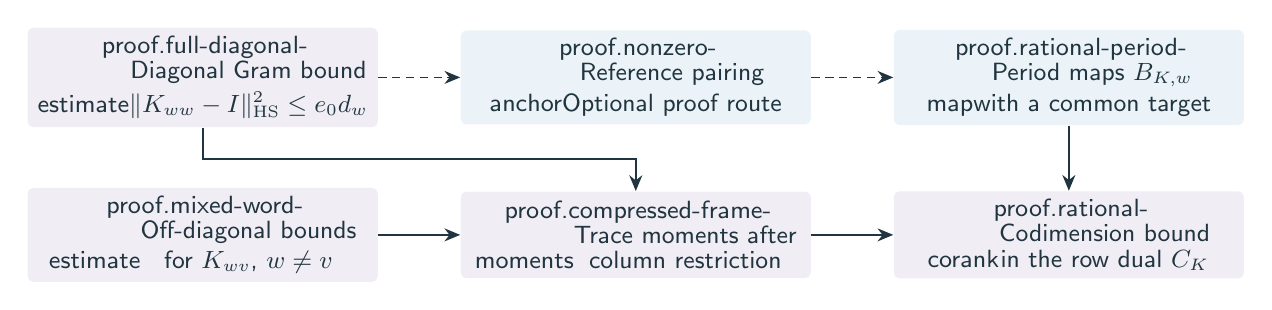
\begin{tikzpicture}[x=1mm,y=1mm]
  \node[argument block,fill=TraceTint] (diagonal) at (0,0)
    {\hyperlink{proof.full-diagonal-estimate}{\shortstack{Diagonal Gram bound\\\(\|K_{ww}-I\|_{\mathrm{HS}}^2\le e_0 d_w\)}}};
  \node[argument block] (anchor) at (55,0)
    {\hyperlink{proof.nonzero-anchor}{\shortstack{Reference pairing\\Optional proof route}}};
  \node[argument block] (periods) at (110,0)
    {\hyperlink{proof.rational-period-map}{\shortstack{Period maps \(B_{K,w}\)\\with a common target}}};
  \node[argument block,fill=TraceTint] (mixed) at (0,-20)
    {\hyperlink{proof.mixed-word-estimate}{\shortstack{Off-diagonal bounds\\for \(K_{wv}\), \(w\ne v\)}}};
  \node[argument block,fill=TraceTint] (compression) at (55,-20)
    {\hyperlink{proof.compressed-frame-moments}{\shortstack{Trace moments after\\column restriction}}};
  \node[argument block,fill=TraceTint] (rational) at (110,-20)
    {\hyperlink{proof.rational-corank}{\shortstack{Codimension bound\\in the row dual \(C_K\)}}};
  \draw[argument arrow,densely dashed] (diagonal.east) -- (anchor.west);
  \draw[argument arrow,densely dashed] (anchor.east) -- (periods.west);
  \draw[argument arrow] (diagonal.south) -- ++(0,-4) -| (compression.north);
  \draw[argument arrow] (mixed.east) -- (compression.west);
  \draw[argument arrow] (compression.east) -- (rational.west);
  \draw[argument arrow] (periods.south) -- (rational.north);
\end{tikzpicture}
\caption{The dashed route gives the reference pairing for an optional
  proof of the granted simultaneous period comparison. There the diagonal
  and ramified rank bounds give \(\dim\ker\mathcal P_w\le e_0d_w<r_w\),
  and full row evaluation pairs with a nonzero image of a ramified
  column. To descend the granted comparison over \(K\), use the compatible
  base pairing and the surjective projected row map over \(K\).
  With the word and dimension estimates, both Gram bounds control the
  trace moments for isometric column inclusions. Using \(J_w=\jmath_w U_w\)
  matches those moments to the period maps. The common projection and
  the distinguished-row dimension bound give the corank over \(K\).}
\label{fig:trace-handoffs}
\end{figure}


\subsection{Unfolding the full Gram operators}
\leavevmode\teamanchor{proof.full-gram-normalization}%
For each \(w\in W\), use the Poincar\'e-series operator
\(\mathcal P_w:H_w^{\mathrm{full}}\to\mathcal H\) in
\eqref{eq:period-gram}. The ambient level and archimedean row type fix
the same finite-dimensional Petersson space \(\mathcal H\) for all
words. Let \(d_w=\dim H_w^{\mathrm{full}}\), \(D=\dim\mathcal H\), and
\(R_{\mathrm{full}}=\sum_w d_w\). The coefficient representation
\(\pi_w\) is the tensor product of the residual compact \(U(k)\)-types
at the real places. Write \(v_N(w)\) for the volume of the unipotent
fundamental domain multiplied by the ambient level volume, and
\(v_H(w)\) for the volume of the real Bessel stabilizer. Then
\(c_0(w)=v_N(w)v_H(w)/\dim\pi_w\), with the measures of
\eqref{eq:period-gram}. Set \(L_w=c_0(w)^{-1/2}\mathcal P_w\) and
\(K_{wv}=L_w^*L_v:H_v^{\mathrm{full}}\to H_w^{\mathrm{full}}\).
The inner product is linear in its second argument.

The orbital formulas in the next paragraphs describe the operators
in the two Gram inputs. Their quantitative estimates are used in the
forms stated at \hyperlink{candidate.diagonal}{the same-word estimate}
and \hyperlink{candidate.trace}{the mixed estimate}.

\leavevmode\teamanchor{proof.gram-unfolding}%
Put \(G_0=U(Y_0)\), where \(Y_0\) has rank \(r=k+m-1\) over the CM
field \(E\), and write \(\mathcal S_w\) for the Bessel subgroup attached to
the flag and its distinguished vector for \(w\). For \(w,v\in W\),
\(\phi\in H_w^{\mathrm{full}}\) and \(\psi\in H_v^{\mathrm{full}}\),
the corresponding Poincar\'e series periodize the seeds
\(\Phi_{w,\phi}\) and \(\Phi_{v,\psi}\), which are invariant under their
respective left rational Bessel subgroup actions, over
\(\mathcal S_w(F)\backslash G_0(F)\) and
\(\mathcal S_v(F)\backslash G_0(F)\), respectively.
Let \(\Omega_{wv}\) be representatives of the rational double cosets
\(\mathcal S_w(F)\backslash G_0(F)/\mathcal S_v(F)\), and set
\(\mathcal S_\gamma(F)=\mathcal S_w(F)\cap\gamma\mathcal S_v(F)\gamma^{-1}\).
Put
\[
 I^+_{wv}(\phi,\psi)=\sum_{\gamma\in\Omega_{wv}}
   \int_{\mathcal S_\gamma(F)\backslash G_0(\mathbf A_F)}
    |\Phi_{w,\phi}(g)|\,|\Phi_{v,\psi}(\gamma^{-1}g)|\,dg,\qquad
 P^+_{w,\phi}(g)=\sum_{\eta\in\mathcal S_w(F)\backslash G_0(F)}
    |\Phi_{w,\phi}(\eta g)|,
\]
with values in \([0,\infty]\). The stabilizer reindexing described
below uses only the left invariance of \(|\Phi_{w,\phi}|\) under
\(\mathcal S_w(F)\) and of \(|\Phi_{v,\psi}|\) under \(\mathcal S_v(F)\).
For nonnegative functions Tonelli's theorem allows it without any
convergence hypothesis, so
\(I^+_{wv}(\phi,\psi)=\int_{G_0(F)\backslash G_0(\mathbf A_F)}
P^+_{w,\phi}P^+_{v,\psi}\,dg\).
By the Cauchy--Schwarz inequality,
\(I^+_{wv}(\phi,\psi)^2\le I^+_{ww}(\phi,\phi)\,I^+_{vv}(\psi,\psi)\).
Absolute convergence for all pairs therefore reduces to the diagonal
pairs, that is, to square integrability of the absolute Poincar\'e
series \(P^+_{w,\phi}\). The edition takes this diagonal finiteness from
the release: at the chosen level ai agent proves
\releasecite{Formalism/LocalToGlobal/SiegelLatticeTheory/FlagStabilizerTensors/LinkSFinal.lean}{97}{absolute convergence}
using the level conditions, neatness and real Whittaker decay.
The release states this finiteness for every pair of words; only its
diagonal instance is used here.
Hence \(I^+_{wv}(\phi,\psi)<\infty\) for all \(w,v,\phi,\psi\). In
particular both Poincar\'e series converge absolutely almost
everywhere, and Fubini's theorem justifies every exchange of sum and
integral in the reindexing. The double-coset unfolding therefore
gives the normalized identity
\[
 \langle\phi,K_{wv}\psi\rangle
   =\frac{1}{\sqrt{c_0(w)c_0(v)}}\sum_{\gamma\in\Omega_{wv}}
     \int_{\mathcal S_\gamma(F)\backslash G_0(\mathbf A_F)}
      \overline{\Phi_{w,\phi}(g)}\Phi_{v,\psi}(\gamma^{-1}g)\,dg .
\]
All quotients carry the measures induced by the adelic Haar measure
in the Petersson product. After unfolding the \(w\) periodization,
the \(v\) sum is indexed by \(\mathcal S_v(F)\backslash G_0(F)\).
The cosets in the double coset of \(\gamma^{-1}\) are represented
by \(\gamma^{-1}a\) for
\(a\in\mathcal S_\gamma(F)\backslash\mathcal S_w(F)\). Integrating
their translates joins the corresponding fundamental domains.
Getz--Hahn use the same stabilizer reindexing for the geometric
side of their relative trace formula with compactly supported tests.
\cite[\S4C, (4C.8) and its unfolding, p.~114]{tr3getzhahn}
ai agent
\releasecite{Formalism/LocalToGlobal/SiegelLatticeTheory/FlagStabilizerTensors/LinkSFinal.lean}{92}{identifies the unfolded coefficients}
using compatible flag and lattice representatives. Separating the
lattices and the finite level conditions gives \(K_{wv}=\sum_t A_t\). In each
coefficient block allowed by the level, \(A_t\) is the archimedean
orbital operator multiplied by the finite character, the level volume
and \((c_0(w)c_0(v))^{-1/2}\). The archimedean operator integrates
\(W_w(g)\otimes W_v(\gamma^{-1}g)^*\), where \(W_w,W_v\) are the
coefficient vectors of the Poincar\'e seeds.

\leavevmode\teamanchor{proof.gram-orbit-expansion}%
Each decorated flag comprises an ordered isotropic frame of length
\(r_S=m/2-1\) and a vector orthogonal to that frame of norm
\(-T_w\) or \(-T_v\). Here \(m\) is even and \(m\ge4\) on the
chosen large-rank family. Set \(a=r_S+1\), and write
\(Z\) for the \(a\)-by-\(a\) matrix of cross pairings of the augmented
frames. With \(e\) the last coordinate vector, their joint Gram matrix
and its determinant are
\[
  M=\begin{pmatrix}-T_w ee^*&Z\\ Z^*&-T_v ee^*\end{pmatrix},
  \qquad
  \det M=(-1)^a G,\qquad
  G=|\det Z|^2-T_wT_v|\det Z_{a-1}|^2 ,
\]
where \(Z_{a-1}\) is the leading \((a-1)\)-by-\((a-1)\) submatrix
and \(|z|^2=z\bar z\) is the CM norm. The determinant follows by swapping
the block columns, taking the Schur complement of \(Z\) and using the
cofactor \(e^*\operatorname{adj}(Z)e\). Polynomiality covers singular
\(Z\). When \(G\ne0\) the augmented
frames span a nondegenerate space of dimension \(2a=m\), since \(m\)
is even. Its orthogonal complement has dimension \(k-1\).

Separate the contribution of the identity double coset, the other
\(G=0\) terms, and the generic and nongeneric terms with \(G\ne0\).
Write \(g_0,g_1\) for the two designated auxiliary rational primes,
which split completely in \(E\). At places above these primes the
finite level uses specific Whittaker characters. A nondegenerate pair
is generic if its lattice in the joint span is generated locally by
the two augmented frames, with the adjusted second frame at the
places above the auxiliary primes. At the identity, the level
calculation for \(w=v\) matches columns and gives \(v_N(w)\). The
average of the unit coefficient vector's rank-one projector over
the real stabilizer commutes with
\(\pi_w\), and its trace is \(v_H(w)\). Schur's lemma gives
\((v_H(w)/\dim\pi_w)I\), so the identity contributes \(I\) to
\(K_{ww}\). For distinct words the calculation at the identity gives
zero by averaging between inequivalent coefficient types.

The unipotent average on the stabilizer quotient vanishes when the
characters disagree on the intersection after transport by \(\gamma\).
Let \(W\) be the joint span of the two augmented frames of a compatible
\(G=0\) orbit and let \(R\) be its radical. The pointwise stabilizer
of \(W\) has reductive quotient \(U(r-\dim W-\dim R)\), since
\(r-\dim W-\dim R\) is the rank of the form on \(W^\perp\). Since \(W\)
contains each augmented frame \(F\), we have \(W^\perp\subseteq
F^\perp\), and this rank is at most the rank \(k\) of the form on
\(F^\perp\). Hence \(\dim W+\dim R\ge m-1\). In the case of equality the
image of \(W^\perp\) in \(F^\perp/\operatorname{rad}F^\perp\) has rank
\(k\), so it is the whole space and the kernel is
\(\operatorname{rad}W^\perp\). The induced map from
\(W^\perp/\operatorname{rad}W^\perp\) is an isometry of
\(k\)-dimensional definite spaces at each real place. The pointwise
stabilizer of \(W\) then maps onto the full residual \(U(k)\) of each
flag, up to fixed unitary conjugation. For such an orbit
Schur's lemma forces the resulting intertwiner to vanish for \(w\ne v\)
because the chosen highest weights differ at every real factor. The next
paragraph shows that equality \(\dim W+\dim R=m-1\) holds for every
compatible orbit with \(G=0\), so this argument covers all of them.

\leavevmode\teamanchor{proof.degenerate-normal-form}%
\paragraph{Compatible orbits with \(G=0\).}
Put \(s=r_S\), so \(m=2s+2\) and \(a=s+1\), and write the two augmented
frames, after transport by \(\gamma\), as \((e_1,\dots,e_s,z)\) and
\((e'_1,\dots,e'_s,z')\) with \(\langle z,z\rangle=-T_w\) and
\(\langle z',z'\rangle=-T_v\). The Hermitian form on \(Y_0\) is taken
linear in the first variable. Put \(X_b=\langle e_1,\dots,e_b\rangle\),
\(X=X_s\), \(X^+=X+Ez\) and \(e_{s+1}=z\), and define \(X'_b\), \(X'\),
\(X'^+\), \(e'_{s+1}=z'\) in the same way. The unipotent group \(N\) of
the first flag consists of the isometries that preserve each \(X_b\),
act trivially on each \(X_b/X_{b-1}\) and act trivially on
\(X^\perp/X\). For \(n\in N\) and \(1\le b\le s\) let \(\lambda_b(n)\)
be the \(e_b\)-coordinate of \(ne_{b+1}-e_{b+1}\in X\). The generic
character has the form \(\psi_N(n)=\psi_E(\sum_b\lambda_b(n))\) for a
nontrivial character \(\psi_E\) of \(\mathbf A_E/E\), as in the release's
definition of compatibility. Only the nontriviality of \(\psi_E\) is
used, and nonzero constant multiples of the \(\lambda_b\) would not
change the argument. Define \(N'\) and \(\psi_{N'}\) in the same way.
Compatibility means \(\psi_N=\psi_{N'}\) on
\((N\cap N')(\mathbf A_F)\). The ambient space has dimension
\(r=k+2s+1\) and negative index \(m/2=s+1\), so signature
\((k+s,s+1)\), at each real place. Choose an isotropic \(X^*\) in
duality with \(X\) and orthogonal to \(z\). Then \(X+X^*\) has
signature \((s,s)\), and the orthogonal complement of \(X+X^*+Ez\) has
signature \((k,0)\). Hence the form on \((X^+)^\perp\) is positive
semidefinite at each real place, with radical \(X\) and positive
definite \(k\)-dimensional quotient. Consequently \((\mathrm P)\) every
isotropic rational vector of \((X^+)^\perp\) lies in \(X\), and no
rational vector of \((X^+)^\perp\) has norm \(-T\) with \(T\) totally
positive. The same holds for the second flag. For \(0\ne x\in X\) the
level is the least \(\ell\) with \(x\in X_\ell\), and the leading
coefficient is its \(e_\ell\)-coordinate. Levels and leading
coefficients for the second flag are defined in the same way.

\emph{Step 1.} Let \(0\ne x\in X\cap X'\) have levels \(\ell,\ell'\) and
leading coefficients \(\alpha,\alpha'\). Then
\(\alpha e_{\ell+1}-\alpha'e'_{\ell'+1}\in X_\ell+X'_{\ell'}\). To see
this, let \(y\) be an adelic vector orthogonal to \(X_\ell+X'_{\ell'}\),
choose \(\eta\in\mathbf A_E\) with \(\eta+\bar\eta=-\langle y,y\rangle\),
and put \(g(u)=u+\langle u,y\rangle x-\langle u,x\rangle y
+\eta\langle u,x\rangle x\). Since \(x\) is isotropic and
\(\langle x,y\rangle=0\), expansion gives
\(\langle gu,gu'\rangle=\langle u,u'\rangle
+\langle u,x\rangle\overline{\langle u',x\rangle}
(\eta+\bar\eta+\langle y,y\rangle)=\langle u,u'\rangle\), so \(g\) is
an isometry. For \(b\le s\) we have \(\langle e_b,x\rangle=0\), so
\(ge_b=e_b+\langle e_b,y\rangle x\). This is \(e_b\) for \(b\le \ell\)
and lies in \(e_b+X_\ell\subseteq e_b+X_{b-1}\) for \(b>\ell\). For
\(u\in X^\perp\), \(gu=u+\langle u,y\rangle x\in u+X\). Hence \(g\in N\),
and likewise \(g\in N'\). Since \(gz-z=\langle z,y\rangle x\) and
\(ge_{b+1}-e_{b+1}=\langle e_{b+1},y\rangle x\), with
\(\langle e_{b+1},y\rangle=0\) for \(b<\ell\) and the \(e_b\)-coordinate
of \(x\) zero for \(b>\ell\), we get
\(\psi_N(g)=\psi_E(\langle\alpha e_{\ell+1},y\rangle)\) and
\(\psi_{N'}(g)=\psi_E(\langle\alpha'e'_{\ell'+1},y\rangle)\). Put
\(u_0=\alpha e_{\ell+1}-\alpha'e'_{\ell'+1}\). Compatibility gives
\(\psi_E(\langle u_0,y\rangle)=1\) for all such \(y\). If a rational
\(y\perp X_\ell+X'_{\ell'}\) had \(\langle u_0,y\rangle\ne0\), replacing
\(y\) by \(ty\) with \(t\in\mathbf A_E\) would make \(\psi_E\) trivial.
Hence \(u_0\perp(X_\ell+X'_{\ell'})^\perp\), and
\(u_0\in X_\ell+X'_{\ell'}\) because the ambient form is nondegenerate.

\emph{Step 2.} First, \(z\notin X+X'\): if \(z=x_1+x_1'\) with
\(x_1\in X\) and \(x'_1\in X'\), then \(x'_1=z-x_1\perp X\) and
\(-T_w=\langle z,z\rangle=\langle x'_1,x'_1\rangle=0\). Likewise
\(z'\notin X+X'\). In Step 1 suppose \(\ell,\ell'<s\), and write
\(u_0=p+p'\) with \(p\in X_\ell\) and \(p'\in X'_{\ell'}\). Then
\(\alpha e_{\ell+1}-p=\alpha'e'_{\ell'+1}+p'\) lies in \(X\cap X'\) and
has levels \(\ell+1,\ell'+1\). If \(\ell=s>\ell'\), Step 1 puts
\(\alpha z\) in \(X+X'\), which is impossible, and \(\ell'=s>\ell\) is
excluded in the same way. Iterating from any nonzero \(x\in X\cap X'\)
therefore gives \(\ell=\ell'\) for every such \(x\), and at the top
level gives \(z'-\theta z\in X+X'\) for some \(\theta\in E^\times\)
whenever \(X\cap X'\ne0\). Let \(j+1\) be the least level of a nonzero
element of \(X\cap X'\), with \(j=s\) if \(X\cap X'=0\). The iteration
produces elements of every level \(j+1,\dots,s\), which are
independent, while \(X\cap X'\cap X_j=0\). Hence
\(\dim(X\cap X')=s-j\), \(X=X_j\oplus(X\cap X')\) and, since the levels
agree, \(X'=X'_j\oplus(X\cap X')\).

\emph{Step 3, \(X\cap X'\ne0\).} Let \(Z_j\) be the leading
\(j\)-by-\(j\) submatrix of \(Z\). The pairing of \(X_j\) with \(X'_j\)
is perfect, so \(\det Z_j\ne0\). Indeed, if \(x\in X_j\) is orthogonal
to \(X'_j\), then \(x\perp X\cap X'\), hence \(x\perp X'\), and
\(x\perp z'\) because \(z'-\theta z\in X+X'\). By \((\mathrm P)\) for
the second flag, \(x\in X'\), so \(x\in X\cap X'\cap X_j=0\). Thus
\(Q=X_j+X'_j\) is nondegenerate of dimension \(2j\). Choose \(h\in X_j\)
with \(\tilde z=z-h\perp X'_j\). Then \(\tilde z\perp Q\),
\(\tilde z\perp X\cap X'\) and \(\langle\tilde z,\tilde z\rangle=-T_w\).
Since \(z'\in\theta z+X+X'\), we get
\(W=Q\oplus(X\cap X')\oplus E\tilde z\), orthogonally, with
\(X\cap X'\) isotropic. So \(R=X\cap X'\), \(\dim W=s+j+1\) and
\(\dim R=s-j\).

\emph{Step 3, \(X\cap X'=0\).} Here compatibility is not needed. If
\(\det Z=0\), some nonzero \(u=x+\beta z\) with \(x\in X\) is
orthogonal to \(X'^+\). If \(\beta=0\), \((\mathrm P)\) gives \(x\in
X'\), so \(x=0\). Otherwise we may take \(\beta=1\), and then
\(\langle u,u\rangle=-T_w\), contrary to \((\mathrm P)\). So
\(\det Z\ne0\), and \(G=0\) forces \(\det Z_s\ne0\), where
\(Z_s=Z_{a-1}\). Then \(X\) and \(X'\) are in perfect pairing, and
\(Q=X\oplus X'\) is nondegenerate. Let \(\tilde z=z-h\) and
\(\tilde z'=z'-h'\), with \(h\in X\) and \(h'\in X'\), be the components
orthogonal to \(Q\). Their norms are \(-T_w\) and \(-T_v\). The Gram
determinant of the augmented frames is \(\pm|\det Z_s|^2\) times that
of \((\tilde z,\tilde z')\). So \(G=0\) makes the latter singular, and
some \(y=\tilde z'-\mu\tilde z\) is orthogonal to \(\tilde z\) and
\(\tilde z'\). The coefficient of \(\tilde z'\) cannot vanish, because
\(\tilde z\) is not isotropic. Then \(y\) is isotropic, orthogonal to
\(Q\) and to \(z\), so \(y\in X\subseteq Q\) by \((\mathrm P)\), and
therefore \(y=0\). Hence \(W=X\oplus X'\oplus E\tilde z\) is
nondegenerate, \(R=0\) and \(\dim W=2s+1\).

In both cases \(\dim W+\dim R=2s+1=m-1\), and the Schur argument above
gives the vanishing for \(w\ne v\).

The mixed block
 consists of the generic and nongeneric sums with
\(G\ne0\) in the same weights and measures.

\subsection{The single-word estimate}

Put \(f=[F:\mathbf Q]\) and \(b=\exp(x^\varepsilon)\). The reference
dimension is
\[
 D_\star=\frac{\mathfrak d V_G}{v^\dagger}>0,
\]
where \(\mathfrak d\) is the product of the target formal degrees,
\(V_G\) is the ambient adelic volume and \(v^\dagger\) is the deep
ambient level volume. These are the measures of the Bessel realization.
For the common factor \(\Gamma=\exp(C_\Gamma m^5 f\log b)\), with
\(C_\Gamma>0\) fixed on the family, the column-size output of the
selection in Section~\ref{sec:assembly} is
\begin{equation}
 \label{eq:trace-balance}
 C_0^{-1}\le \frac{d_w\Gamma^2}{D_\star}\le C_0
 \qquad(w\in W), \qquad C_0\ge1.
\end{equation}
The selected constant is \(C_0=3\). The balanced dimensions here count
the full level-zero columns before cutting by the word-prime
characters. Since \(D_\star>0\), the lower bound makes every \(d_w\)
positive. The selected rank inequalities give \(m^4\le f\le k\le x^5\)
and \(k\ge 8\log\Gamma\) at all sufficiently large scales.

The level index explains the balance. Let \(d_w^{(0)}\) be the compact
column dimension before marking a nonzero covector at each place
above \(T_w\), with the two auxiliary levels and the word's real
type retained. Let \(K_0\) be this compact level and \(K_0'\subset K_0\)
the subgroup of elements whose reduction at each place above \(T_w\)
fixes the marked nonzero covector. Reduction onto
\(\mathrm{GL}_k(\mathbf F_{T_w})\) is surjective, and this group acts
transitively on the \(T_w^k-1\) nonzero covectors. By the
orbit--stabilizer theorem, \([K_0:K_0']=(T_w^k-1)^f\).
For a class \(G(F)gK_0\), the classes of level \(K_0'\) above it are
in bijection with the orbits of \(g^{-1}\Gamma_gg\) on \(K_0/K_0'\),
where \(\Gamma_g=G(F)\cap gK_0g^{-1}\). This group is finite by
definiteness.
At a place above the auxiliary prime \(g_i\), the level consists of
elements with upper unitriangular reduction. The preimage of the
unitriangular group is pro-\(g_i\), because the principal congruence
kernel is pro-\(g_i\), and so is each conjugate of it. Hence every
element of \(\Gamma_g\) has order a power of \(g_0\) and a power of
\(g_1\), so \(\Gamma_g=1\). The same holds for the stabilizers at level
\(K_0'\). Thus every class of level \(K_0\) has exactly
\((T_w^k-1)^f\) classes above it, and every class at either level
carries the full residual fibre. Counting fibres gives
\[
 d_w=(T_w^k-1)^f\,d_w^{(0)} .
\]
For comparison, the release records this index as
\releasecite{Formalism/SharpRestriction/GlobalSchurBounds/StandardLattice.lean}{446}{The level index and compact rank}.
Write
\[
 Y_w=\left(\frac{D_\star}{d_w^{(0)}\Gamma^2}\right)^{1/(fk)}.
\]
The word-prime interval is \(Y_w\le T_w\le Y_w(1+1/(fk))\). It is
the auxiliary-level choice of Section~\ref{sec:integral}, which the
edition takes from the release there. In that choice
\(d_w^*\) is the coefficient of \((T_w^k-1)^f\) in the full column
dimension, so \(d_w^*=d_w^{(0)}\) by the index formula, and the chosen
interval \(1\le T_w/(X_w\Gamma^{-2/(fk)})\le1+1/(fk)\) reads
\(Y_w\le T_w\le Y_w(1+1/(fk))\) because
\(X_w\Gamma^{-2/(fk)}=Y_w\). The release records the same interval in
the chosen record at
\releasecite{Formalism/LocalRingCardinality/RhoDetPrimeEqMuTildeMulChiPow.lean}{153}{The word-prime interval}.
Thus the exact ratio \(d_w\Gamma^2/D_\star\) is
\((T_w^k-1)^f/Y_w^{fk}=(T_w/Y_w)^{fk}(1-T_w^{-k})^f\). Its upper bound
is \((1+1/(fk))^{fk}\le\exp(1)<3\). By Bernoulli's inequality its lower
bound is \(1-fT_w^{-k}\ge1-x^5b^{-k}\ge1/2>1/3\) for large \(x\), since
\(T_w\ge b\) and \(f\le x^5\). Given the interval, this proves
\eqref{eq:trace-balance} with \(C_0=3\).
The count uses the same \(D_\star\) as the row projector below.

\leavevmode\teamanchor{proof.full-diagonal-estimate}%
With the contribution \(I\) of the identity removed, there are two
sums in \(K_{ww}-I\): the sum \(K_{\rm deg}\) over the nonidentity
orbits with \(G=0\), and the sum \(K_{\rm nd}=K_{\rm gen}+K_{\rm ng}\)
over the generic and nongeneric orbits with \(G\ne0\). We show
\(\|K_{\rm deg}\|_{\rm HS}^2\le d_w\exp(-kf\log k)\) and
\(\|K_{\rm nd}\|_{\rm HS}^2\le\Gamma d_w^2/D_\star\). Throughout,
\(\log P_g\le6b^{-7}\), as in the
\hyperlink{proof.mixed-word-estimate}{mixed-word estimate}, so
\(P_g\le2\).

\paragraph{The degenerate sum.}
\teamanchor{proof.degenerate-diagonal-sum}%
Group the nonidentity \(G=0\) terms into rows as in the
\hyperlink{proof.quadratic-row-contraction}{quadratic row contraction},
with \(w=v\). The
\hyperlink{proof.squared-norm-identity}{derivation of the squared norm}
applies verbatim to this family \(\mathcal S\). It uses the character
factorization, the constant unipotent factor and the free column
decompositions, which concern single terms, their lattice pairs and
their column representatives and not the family. It also uses the left
and right Gram invariance, whose cited release statements are made
for each of the generic, nongeneric and nonidentity degenerate
families, and the absolute summability, which covers all orbit terms.
Hence
\(\|K_{\rm deg}\|_{\rm HS}^2=\operatorname{Re}\sum_{i,j}\mathcal G_{ij}
\langle V_i,V_j\rangle\), with \(V_i\) formed from the degenerate terms.
The Gelfand--Graev bound
\(0\le\mathcal G\le P_g\Gamma_1\operatorname{Id}\) proved there gives,
by the same coordinate argument,
\[
 \|K_{\rm deg}\|_{\rm HS}^2
 \le P_g\Gamma_1\sum_{\substack{t,t'\ {\rm deg}\\ r(t)=r(t')}}
     \|v_t\|\,\|v_{t'}\|.
\]
The right side satisfies the following typed amplitude bound, which is
assembled below from release inputs. There is a constant \(C_A\ge1\),
fixed on the family, such that
\[
 \Gamma_1\sum_{\substack{t,t'\ {\rm deg}\\ r(t)=r(t')}}
     \|v_t\|\,\|v_{t'}\|
 \le d_w\Bigl(\sum_{j=1}^{r_S}\alpha_j\Bigr)^2,\qquad
 \alpha_j=\exp(C_Am^6f\log b)\Bigl(\frac{C_A}{k}\Bigr)^{j(k-1-j)f}.
\]
The numerics after this bound are given at the end of the assembly.

\leavevmode\teamanchor{proof.degenerate-amplitude-assembly}%
\paragraph{Assembly of the typed amplitude bound.}
Call a degenerate term relevant if its orbit is compatible in the sense
of the \hyperlink{proof.degenerate-normal-form}{normal form}. The
assembly uses six inputs.

(i) An irrelevant term has \(v_t=0\): its orbital integral contains
the unipotent average, which vanishes when the characters disagree, as
stated in the \hyperlink{proof.gram-orbit-expansion}{orbit expansion}.
The edition takes this vanishing of the irrelevant degenerate vectors
from the release
\releasecite{Formalism/LocalToGlobal/SiegelLatticeTheory/CokernelGLCounts/RankPointCounts/CovolumeSpans.lean}{35}{vanishing of the irrelevant degenerate vectors}.

(ii) A relevant term has \(1\le j(t)\le r_S\). Here \(j(t)\) is the
index \(j\) of the normal form, so \(\dim(X\cap X')=r_S-j(t)\) and the
upper bound holds by definition. Suppose \(j(t)=0\). Then
\(\dim(X\cap X')=r_S\), so \(X=X'\). By Step~2 every nonzero
\(x\in X\) has the same level for both flags, so \(X'_b=X_b\) for every
\(b\). Since \(r_S\ge1\), Step~2 also gives \(z'-\theta z\in X\) with
\(\theta\in E^\times\), so \(X'^+=X^+\). Since \(w=v\), \(z\perp X\) and
\(X\) is isotropic, comparing \(\langle z',z'\rangle\) with
\(\langle z,z\rangle\) gives \(\theta\bar\theta=1\). The release shows
that a relevant term whose flags have equal subspaces \(X_b\) and equal
\(X^+\) is the identity term, using that the word prime \(T_w\) is
prime to \(g_0g_1\)
\releasecite{Formalism/LocalToGlobal/SiegelLatticeTheory/CokernelGLCounts/RankPointCounts/IsIdentityOfEqualFlags.lean}{20}{identity recognition for equal flags}.
The argument there runs as follows. The comparison scalar is a unit
with all absolute values one, hence a root of unity. Admissibility of
the lattice data makes it congruent to \(1\) modulo the primes above
\(g_0\) and \(g_1\), hence equal to \(1\), and the term is then
realised by an element of the unipotent group of the lattice. The identity term is excluded from the
degenerate family, so \(j(t)\ge1\).

(iii) The typed real amplitude bound. Set \(H_c=b^{cm^2f}\) and
\(H_1=b^{C_Hm}\). A relevant term \(t\) has a label
\(\delta=(\delta_l)_l\), the local comparison data of its two flags at
the levels \(l\le j(t)\), with \(\delta_l=0\) for \(l>j(t)\). Let
\(\Delta(t)\) be the absolute norm of the local discriminant attached
to \(\delta_{j(t)}\). Put
\(S(t)=\prod_\tau\max\bigl(1,\max_l|\delta_l|_\tau/(2H_1)^{2r_S}\bigr)\ge1\),
where the product runs over the real places \(\tau\) of \(F\) and
\(|\delta_l|_\tau\) is the archimedean size of the label entry. The
release gives constants \(C_H,C_h,C_p\ge0\) with the following
property. For every \(C_s\ge C_p+4\) and every sufficiently large
\(C\ge0\), each finite set of same-row ordered pairs of relevant terms,
in which the first terms all have type \((j',\delta')\) and the second
terms all have type \((j'',\delta'')\), satisfies
\[
 \sum\|v_t\|\,\|v_{t'}\|\le\dim\pi_w\,M_w\,
   (ae)(j',\delta')\,(ae)(j'',\delta'').
\]
Here
\(a(j,\delta)=(C/k)^{j(k-1-j)f}\Delta^{-(k-1-j)/2}H_C^{Cr_S^4}S^{-C_sk}\)
and \(e(j,\delta)=\Delta^{k/2}H_{C_h}^{C_hr_S^4}S^{C_pk}\),
\(\pi_w\) is the fibre representation of the columns of \(w\), and
\(M_w=\sum_\Lambda|A_\Lambda|^{-1}\) is the total lattice weight
\releasecite{Formalism/LocalToGlobal/SiegelLatticeTheory/FlagStabilizerTensors/RowsPos.lean}{18}{typed real amplitude bound}.

(iv) \(0<\Delta(t)\le H_CS(t)^2\) for the same \(C\)
\releasecite{Formalism/LocalToGlobal/SiegelLatticeTheory/CokernelGLCounts/RankPointCounts/DimFormC.lean}{65}{discriminant bound}.

(v) There is \(C_c\ge0\) such that for each \(1\le j\le r_S\) and each
finite set \(T\) of labels realised by relevant terms of rank \(j\),
\(\sum_{\delta\in T}S^{-3r_S}\le H_{C_c}^{C_cr_S}\)
\releasecite{Formalism/LocalToGlobal/SiegelLatticeTheory/CokernelGLCounts/RankPointCounts/DimFormC.lean}{72}{coset count}.

(vi) The dimension formula \(\Gamma_1M_w\dim\pi_w\le d_w\)
\releasecite{Formalism/LocalToGlobal/SiegelLatticeTheory/CokernelGLCounts/RankPointCounts/DimFormC.lean}{80}{dimension formula}.

The constants are fixed in the order \(C_H,C_h,C_p\), then
\(C_s=C_p+4\), then \(C\) large for (iii) and (iv), then \(C_c\), and
finally \(C_A=1+C+C^2+C_h^2+C_c^2\). The assembly is now algebra. The
exponents of \(\Delta\) add to \((j+1)/2\), so
\[
 (ae)(j,\delta)=(C/k)^{j(k-1-j)f}H_C^{Cr_S^4}H_{C_h}^{C_hr_S^4}
   \Delta^{(j+1)/2}S^{(C_p-C_s)k}.
\]
By (iv), \(\Delta^{(j+1)/2}\le H_C^{(j+1)/2}S^{j+1}\). Since \(S\ge1\),
\(C_s-C_p\ge4\) and \(j+1+3r_S\le4r_S+1\le4k\), we get
\(S^{j+1+(C_p-C_s)k}\le S^{-3r_S}\). Summing over a finite set of
labels of rank \(j\) with (v) gives
\[
 \sum_\delta(ae)(j,\delta)\le\tilde\alpha_j=(C/k)^{j(k-1-j)f}
   H_C^{Cr_S^4+(j+1)/2}H_{C_h}^{C_hr_S^4}H_{C_c}^{C_cr_S}.
\]
Now take a finite set of same-row ordered pairs of nonidentity
degenerate terms. Pairs with an irrelevant member contribute \(0\) by
(i). By (ii), the rest split by \((j',\delta',j'',\delta'')\) with
\(1\le j',j''\le r_S\), and only finitely many labels occur. Applying
(iii) to each piece and summing over labels gives the bound
\(\dim\pi_w\,M_w(\sum_{j=1}^{r_S}\tilde\alpha_j)^2\). Absolute summability lets
the finite set exhaust the sum. Finally
\(H_c^y=\exp(cym^2f\log b)\), and \(r_S\le m\), \((j+1)/2\le m\) give
\(C^2r_S^4+C(j+1)/2+C_h^2r_S^4+C_c^2r_S\le C_Am^4\). Since
\(0\le C\le C_A\) and \(j(k-1-j)\ge0\), this gives \(\tilde\alpha_j\le\alpha_j\).
Multiplying by \(\Gamma_1\) and using (vi) gives the typed amplitude
bound.

The remaining numerics are as follows. Since \(m=2r_S+2\) and
\(k\ge m+3\), each \(1\le j\le r_S\) has \(j(k-1-j)\ge k-2\). Beyond a
scale threshold, \(\log k\ge8\log C_A\) and
\(k\log k\ge8C_Am^6\log b\). Indeed \(k\ge70\log b\) tends to
infinity, and \(k\ge8C_\Gamma m^5f\log b\ge8C_\Gamma m^9\log b\), so
the second inequality holds once \(C_\Gamma\log k\ge C_A\). Then
\(C_A/k\le1\), \(r_S\le k\), and
\[
 \log\Bigl(2\Bigl(\sum_j\alpha_j\Bigr)^2\Bigr)
 \le\log2+2\log k+2C_Am^6f\log b-2(k-2)f\log k+2(k-2)f\log C_A .
\]
The last two positive terms are each at most \(\tfrac14kf\log k\), and
\(\log2+2\log k\le3f\log k\). The right side is therefore at most
\((7-\tfrac32k)f\log k\le-kf\log k\), since \(k\ge14\). With
\(P_g\le2\) this gives \(\|K_{\rm deg}\|_{\rm HS}^2\le d_w\exp(-kf\log k)\).

\paragraph{The nondegenerate sum.}
\teamanchor{proof.equal-word-nondegenerate}%
The \hyperlink{proof.quadratic-row-contraction}{quadratic row contraction},
the \hyperlink{proof.orbital-error-estimates}{orbital error estimates}
and the combination in the
\hyperlink{proof.mixed-word-estimate}{mixed-word estimate} apply with
\(v=w\), with one change: the scalar main term. Put
\(D_{ww}=d_w^2/D_\star\). The edition takes the following equal-word
scalar bound from the release
\releasecite{Development/AbelianVarietyTheory/Proofs/FlagMeasures/RowMainEqPOfSiegelWeil.lean}{10}{Siegel--Weil}.
The signed sum over the generic scalar pairs of \(K_{ww}\), weighted by
\(\Gamma_1\) as in the finite convolution, is at most
\(\Gamma_BD_{ww}\), with \(\Gamma_B=\exp(C_Bm^5f\log b)\) for a
constant \(C_B\ge0\) fixed on the family. The release does not prove
this by the positivity and Poisson argument of the
\hyperlink{proof.scalar-row-normalization}{scalar normalization}, and
the edition does not use the bound \(AD_{wv}\) of that argument with
\(v=w\). Instead, the release groups the generic scalar pairs into
classes and, within a class, by a rational point and a normal datum.
It bounds each class by Cauchy--Schwarz and a mean bound for the local
generic amplitudes, and counts the points and normals with height
weights
\releasecite{Formalism/LocalToGlobal/SiegelLatticeTheory/CokernelGLCounts/RankPointCounts/MainEqCut.lean}{195}{class, amplitude and height bound for generic scalar pairs}.
Only then is the sum normalized. The Siegel--Weil formula, with the
local Bessel integral from Section~\ref{sec:periods} in both word slots
of the real orbital integral, enters through the equal-word mass data.
These mass data bound the \(\Gamma_1\)-weighted archimedean mass by
the scale \(d_wd_v/D_\star\) of the distinct-word normalization, now
taken at \(v=w\), times a factor that depends only on the field
discriminant, the auxiliary primes and the rank
\releasecite{Formalism/LocalToGlobal/SiegelLatticeTheory/CokernelGLCounts/RankPointCounts/MainEqCut.lean}{259}{normalization of the class bound by the mass data}.
The scale \(D_{ww}\) is the only thing the edition takes from the
scalar normalization at \(v=w\). This factor and the class and height
counts are absorbed into \(\Gamma_B\), which is why the bound is crude. It
suffices, because \(\Gamma\ge\Gamma_Bb^{m^5f}\) below. The error bounds
\(\epsilon_LD_{ww}\) and \(\epsilon_ND_{ww}\) are also taken for
\(v=w\); their release statements cover every pair of words.
The identity orbit has \(G=0\), so it lies in neither family. As in
the mixed-word estimate,
\[
 \|K_{\rm nd}\|_{\rm HS}^2
 \le D_{ww}\Bigl[\sqrt{P_g(\Gamma_B+2\epsilon_L)}
    +\sqrt{P_g(\epsilon_L+\epsilon_N)}\Bigr]^2 .
\]
The release
\releasecite{Formalism/LocalToGlobal/SiegelLatticeTheory/FlagStabilizerTensors/RowsPos.lean}{210}{combines these equal-word pair estimates}
in the same way. To bound the bracket put
\(E=\exp(\max(C_B,C_N)m^5f\log b)\ge1\). Then \(\Gamma_B\le E\),
\(\epsilon_L\le1\), and \(\epsilon_N\le E\) because
\(k\ge2r_S+5\). Using \((\sqrt a+\sqrt c)^2\le2(a+c)\) and \(P_g\le2\),
the bracket is at most \(4(\Gamma_B+3\epsilon_L+\epsilon_N)\le20E\).
The constants \(C_B\) and \(C_N\) are fixed first, and the family
exponent is chosen with
\[
 C_\Gamma\ge\max(C_B,C_N)+1 .
\]
Then \(\Gamma\ge E\,b^{m^5f}\), and \(b^{m^5f}\ge16^{512}>20\) because
\(b\ge16\), \(m\ge2\) and \(f\ge m^4\). Hence
\(\|K_{\rm nd}\|_{\rm HS}^2\le\Gamma d_w^2/D_\star\).
The rank thresholds are taken after \(C_\Gamma\), and the rank
satisfies \(k\ge 8C_\Gamma m^5f\log b\).

The upper ratio in \eqref{eq:trace-balance} gives
\(\Gamma d_w^2/D_\star\le(C_0/\Gamma)d_w\).
Combining the degenerate and nondegenerate estimates
by the squared triangle inequality
\(\|A+B\|^2\le2\|A\|^2+2\|B\|^2\) gives
\begin{equation}
 \label{eq:trace-single-diagonal}
 \|K_{ww}-I\|_{\mathrm{HS}}^2\le e_0 d_w,\qquad
 e_0=2\exp(-kf\log k)+2C_0/\Gamma .
\end{equation}
Here \(k\ge 8\log\Gamma\) and \(\log\Gamma\ge C_\Gamma x^\varepsilon\), so
\(\sqrt{e_0}\le\exp(-x^{\varepsilon/8})\) for large \(x\), uniformly
over the selected translates.

\noindent\leavevmode\teamanchor{candidate.diagonal}%
\textbf{AI-proposed candidate (the same-word Gram defect).}
Fix the target, precision and tied family with its levels, weight
gaps and rank conditions, including \eqref{eq:trace-balance} and
\(k\ge8\log\Gamma\), with \(C_\Gamma\ge\max(C_B,C_N)+1\) for the
fixed constants \(C_B\) of the equal-word scalar bound and \(C_N\) of
the nongeneric estimate. At every selected translate beyond one common
scale threshold, the full Gram operator of each word has mean
squared defect
\[
 \frac{\|L_w^*L_w-I\|_{\rm HS}^2}{d_w}
 \le 2e^{-kf\log k}+\frac{2C_0}{\Gamma},
 \qquad \Gamma=\exp(C_\Gamma m^5 f\log b).
\]
The normalization gives \(I\) on the identity double coset. The
estimate uses absolute bounds for the remaining degenerate terms
and the equal-word nondegenerate bound \(\Gamma d_w^2/D_\star\),
\hyperlink{proof.full-diagonal-estimate}{derived above} from the
release inputs named there.
This nondegenerate calculation shares orbital estimates with the
mixed-word proof below. The same-word statement controls the mean
of \((\sigma_j^2-1)^2\) over the \(d_w\) singular values of \(L_w\),
including zeros. Mixed bounds alone allow mutually orthogonal
images with each \(L_w\) twice an isometric inclusion, for which
the mean squared defect is \(9\).

Wei obtains a growing matrix of \(qI_2\)-Fourier coefficients of
the \(pI_2\) Siegel Poincar\'e series, with main term \(8I\) and
an entrywise error decreasing faster than any power of the weight.
\cite[Lemma~2.3 and \S3.1]{tr3wei-poincare}
The estimate above treats all full Bessel columns of one word
in the unitary family, with the indicated dependence on its rank,
field and level.

\leavevmode\teamanchor{proof.ramified-column-loss}%
The period source \(H_w^{\mathrm{act}}=\mathcal M_w\) is the ramified
column space included by \(\jmath_w\) in Section~\ref{sec:periods}.
At level zero the columns are sections over the definite class set,
with one residual compact representation fibre per class. Since \(T_w\)
splits completely in \(E\), there are \(f\) places of \(F\) over it
and the \(T_w\)-diamond group is
\(\mathsf A_w=\prod_{z\mid T_w}\mathbf F_{T_w}^{\times}\).
It acts by right translation on the classes and carries the fibres
isomorphically along this action. A diamond representative is an
integral local dilation at the \(T_w\)-places and the identity at
the auxiliary places. If it fixes a class, the double-coset equation
identifies its product with a level element with a rational point
preserving the lattice of that class. This rational stabilizer is
finite by definiteness. At each auxiliary prime the reduction is
upper unitriangular, and the preimage of that group is pro-\(g_i\)
because the principal congruence kernel is pro-\(g_i\). Thus the
stabilizer element has order a power of each of two distinct primes.
It is the identity, so the diamond representative is itself in the
level and acts by the trivial multiplier at every \(T_w\)-place.
For comparison, the release proves the same freeness at
\releasecite{Formalism/LocalToGlobal/GlobalTheory/GL6/DiagonalSlopes/EqOneOfCoprimeTorsionTwoPrimes.lean}{670}{Freeness at the level-zero classes}.

On each free orbit fix an identification of the fibre at one class
and transport it by the group action. This identifies the full
column representation over the orbit with the regular representation
of \(\mathsf A_w\) tensored with that fibre. In each
\(\mathbf C[\mathbf F_{T_w}^{\times}]\) the kernel of the local
averaging projector has dimension \(T_w-2\). The actual ramified
space is the intersection of these local kernels. Its restriction
to the orbit is the tensor product of the individual kernels with
the fibre, since the \(f\) local projections act in distinct factors.
Adding the ranks over the orbits therefore gives the first equality
below. With \(r_w=\dim\mathcal M_w\) and \(T_w\ge b\ge3\), Bernoulli's
inequality gives the rest:
\begin{equation}
 \label{eq:trace-ramification}
 r_w=d_w\left(1-\frac1{T_w-1}\right)^f,\qquad
 0\le d_w-r_w\le\frac{2f}{b}d_w.
\end{equation}
This is the ratio for the same level-zero columns counted in
\eqref{eq:trace-balance}.
For comparison, the release states the same formula at
\releasecite{Formalism/SharpRestriction/GlobalSchurBounds/FiniteModelOfAdmissibleTransports.lean}{842}{Ramified rank formula}.

The diagonal input gives another use of this calculation.
On \(\ker\mathcal P_w\), the operator \(K_{ww}-I\) is \(-I\).
Consequently \(\dim\ker\mathcal P_w\le e_0 d_w\). The bound
\(f\le k\le x^5\) implies \(e_0<1-2f/b\) for sufficiently large \(x\),
so some vector in \(\mathcal M_w\) has nonzero image under
\(\mathcal P_w\). Pairing with that image in the full \(\mathcal H\)
supplies the nonzero bottom pairing.

In the construction of the bottom reference pairing, the
\releasecite{Development/AbelianVarietyTheory/Proofs/DecoratedLatticeProofs/DiagonalRowOfSiegelWeilUnitary.lean}{50}{earlier single-word estimate}
comes from the same local Bessel integrals and Siegel--Weil. In
combination with the ramified rank bound, it puts the squared diagonal
defect strictly below the dimension of the ramified column space of
each such bundle. The
\releasecite{Development/AutomorphicArithmetic/ThetaCorrespondence/ThetaPairLifts/ThirdPlaceSeries/MainTheoremPublishedResultsFinal.lean}{34}{formal construction}
uses this inequality to obtain a nonzero image of a ramified column.
For the conditional argument we use the period maps supplied by
\hyperlink{candidate.periods}{the stated comparison}.

\subsection{Squaring the orbital sum at finite level}
\leavevmode\teamanchor{proof.quadratic-row-contraction}%
Fix \(w\ne v\) and let \(\mathcal S\) be either of the two orbit
families with \(G\ne0\). The same grouping applies with \(w=v\). The
identity orbit has \(G=0\) and lies in neither family. The resulting
equal-word bound \(\Gamma d_w^2/D_\star\) is derived in the
\hyperlink{proof.equal-word-nondegenerate}{single-word estimate} from
the release inputs named there. Group the terms by their two lattice
representatives and the remaining index \(i(t)\) in the finite Levi
group. Call this triple the row \(r(t)\). At a place of \(F\) above
\(g_0g_1\) with residue size \(q\), the group is
\(G_q=\mathrm{GL}_k(\mathbf F_q)\) with upper unitriangular subgroup
\(U_q\). Write \(I=\prod_q G_q\), with all such products indexed by
these places. The weighted vector \(v_t\) is the normalized real
orbital operator in the Hilbert--Schmidt summand for its lattice pair,
multiplied by the finite unipotent character and the square root of
the product of the two lattice weights.
Put \(K_{\mathcal S}=\sum_{t\in\mathcal S}A_t\) and
\(V_i=\sum_{t\in\mathcal S:\,i(t)=i}v_t\).
In the chosen column representatives the unipotent factor of the
finite character is constant for each lattice pair. The remaining
factor is the character of \(\prod_q U_q\), extended by zero, evaluated
at the relative Levi index for the two column representatives. The
representatives give free decompositions of \(I\), and the Gram sums
for each family are invariant under the corresponding left and right
translations in \(I\). The edition takes these structural facts
from the release:
\releasecite{Formalism/LocalToGlobal/SiegelLatticeTheory/ClosedLocalOrbits/GaugeLatticeShifts/ColPhaseCut.lean}{49}{the character factorization},
\releasecite{Formalism/LocalToGlobal/SiegelLatticeTheory/ClosedLocalOrbits/GaugeLatticeShifts/ChiNCut.lean}{48}{the constant unipotent factor},
\releasecite{Formalism/LocalToGlobal/SiegelLatticeTheory/ClosedLocalOrbits/GaugeLatticeShifts/NormExpSatHolds.lean}{17}{the free column decompositions}
and the left and right Gram invariance
\releasecite{Formalism/LocalToGlobal/SiegelLatticeTheory/ClosedLocalOrbits/GaugeLatticeShifts/NormExpSatHolds.lean}{23}{left invariance}
\releasecite{Formalism/LocalToGlobal/SiegelLatticeTheory/ClosedLocalOrbits/GaugeLatticeShifts/NormExpSatHolds.lean}{37}{right invariance}.
The derivation below shows that they give the squared norm
\[
  \|K_{\mathcal S}\|_{\mathrm{HS}}^2
    =\operatorname{Re}\sum_{i,j\in I}\mathcal G_{ij}\langle V_i,V_j\rangle,
  \qquad
  \mathcal G_{ij}=\overline{\prod_q\gamma_q((j^{-1}i)_q)}.
\]
Here \(\gamma_q=\operatorname{ch}(\operatorname{Ind}_{U_q}^{G_q}\psi_q)\)
is the Gelfand--Graev character,
where \(\psi_q\) is the nondegenerate character obtained from the
chosen nontrivial residue-field character on the sum of the simple
superdiagonal entries.

\leavevmode\teamanchor{proof.squared-norm-identity}%
\paragraph{Derivation of the squared norm.}
Take the Hilbert--Schmidt inner product conjugate-linear in the first
variable. Let \(U=\prod_qU_q\), let \(\psi=\prod_q\psi_q\) on \(U\),
extended by zero to \(I\), and let \(\gamma=\prod_q\gamma_q\). Then
\(\psi(ug)=\psi(u)\psi(g)\) and \(\psi(gu)=\psi(g)\psi(u)\) for \(u\in U\)
and \(g\in I\). Fix a
lattice pair \(\Lambda\) occurring in \(\mathcal S\). The structural
facts say the following. The \(\Lambda\)-summand of \(K_{\mathcal S}\)
has, between a column \(\rho\) of the first lattice and a column
\(\rho'\) of the second, the block
\(\sum_t\psi(s_\rho^{-1}i(t)s'_{\rho'})a_t\). The sum runs over
\(t\in\mathcal S\) with lattice pair \(\Lambda\), \(s_\rho,s'_{\rho'}\in
I\) are the column representatives, and \(a_t\) is the remaining factor of \(A_t\): the normalized real
orbital operator times the level volume and the unipotent factor,
which is constant for the lattice pair.
There are subsets \(A_\Lambda,A'_\Lambda\subseteq I\) for which
\((b,\rho,u)\mapsto bs_\rho u\) and \((b,\rho',u)\mapsto bs'_{\rho'}u\)
are bijections onto \(I\) from \(A_\Lambda\times\{\rho\}\times U\) and
\(A'_\Lambda\times\{\rho'\}\times U\), where \(\rho\) and \(\rho'\) run
over the columns of the first and second lattice of \(\Lambda\). The two lattice
weights are \(|A_\Lambda|^{-1}\) and \(|A'_\Lambda|^{-1}\). Finally,
\(Z_\Lambda(i)=\sum_{t:\,i(t)=i}a_t\) satisfies
\(\langle Z_\Lambda(bi),Z_\Lambda(bj)\rangle
=\langle Z_\Lambda(i),Z_\Lambda(j)\rangle\) for \(b\in A_\Lambda\) and
\(\langle Z_\Lambda(ib^{-1}),Z_\Lambda(jb^{-1})\rangle
=\langle Z_\Lambda(i),Z_\Lambda(j)\rangle\) for \(b\in A'_\Lambda\).
The sums over \(t\) converge absolutely in the Hilbert--Schmidt norm
\releasecite{Formalism/LocalToGlobal/SiegelLatticeTheory/ClosedLocalOrbits/GaugeLatticeShifts/KExpCut.lean}{301}{absolute summability of the orbit terms},
which justifies the regrouping below.
In the release this summability is deduced from three facts: each
block of a term has norm at most a fixed volume factor times the
operator norm of the orbital integral of that term
\releasecite{Formalism/LocalToGlobal/SiegelLatticeTheory/ClosedLocalOrbits/GaugeLatticeShifts/KExpCut.lean}{95}{block bound},
this operator norm is at most the integral, over the fundamental
domain of the term at the real places, of the product of the norms of
the two coefficient vectors \(W_w\) and \(W_v\)
\releasecite{Formalism/LocalToGlobal/SiegelLatticeTheory/ClosedLocalOrbits/GaugeLatticeShifts/DoubleCosetSingleUnfolding.lean}{383}{norm of an orbital integral},
and these absolute integrals have a finite sum over the terms
\releasecite{Formalism/LocalToGlobal/SiegelLatticeTheory/ClosedVolumeStatements/FullExistsTiedHolds.lean}{27}{absolute convergence over the terms}.
The terms there are indexed by lattice pairs and adelic classes modulo
the lattice unipotent subgroups. This indexing refines the rational
double cosets of the unfolding, so the edition does not deduce the last
finiteness from the absolute convergence proved for the unfolding.
The Hilbert--Schmidt norm is additive over blocks, so
\[
  \|K_{\mathcal S}\|_{\mathrm{HS}}^2=\sum_\Lambda\sum_{\rho,\rho'}
   \Phi_\Lambda(s_\rho,s'_{\rho'}),\qquad
  \Phi_\Lambda(x,y)=\sum_{i,j\in I}
   \overline{\psi(x^{-1}iy)}\,\psi(x^{-1}jy)\,
   \langle Z_\Lambda(i),Z_\Lambda(j)\rangle .
\]
Replacing \(x\) by \(xu\) or \(y\) by \(yu\) with \(u\in U\) multiplies
the summand by \(|\psi(u)|^2=1\). Replacing \(x\) by \(bx\) with
\(b\in A_\Lambda\), or \(y\) by \(by\) with \(b\in A'_\Lambda\), is
undone by substituting \(i\mapsto bi\), \(j\mapsto bj\), or
\(i\mapsto ib^{-1}\), \(j\mapsto jb^{-1}\), and using the Gram
invariance. By the free decompositions,
\[
  \sum_{\rho,\rho'}\Phi_\Lambda(s_\rho,s'_{\rho'})
   =\frac{1}{|A_\Lambda||A'_\Lambda||U|^2}\sum_{x,y\in I}
     \Phi_\Lambda(x,y).
\]
In the sum over \(y\), substitute \(y\mapsto i^{-1}xy\). The term
\(\overline{\psi(y)}\psi(x^{-1}ji^{-1}xy)\) vanishes unless \(y\in U\)
and \(x^{-1}ji^{-1}x\in U\), and then it equals
\(\psi(x^{-1}ji^{-1}x)\). The Frobenius formula
\(\gamma(g)=|U|^{-1}\sum_{x\in I}\psi(x^{-1}gx)\) then gives
\(\sum_{x,y}\overline{\psi(x^{-1}iy)}\psi(x^{-1}jy)=|U|^2\gamma(ji^{-1})\).
Since \(\gamma\) is a class function and \(\gamma(g^{-1})
=\overline{\gamma(g)}\), we have \(\gamma(ji^{-1})=\gamma(i^{-1}j)
=\mathcal G_{ij}\). Hence
\[
  \|K_{\mathcal S}\|_{\mathrm{HS}}^2=\sum_{i,j}\mathcal G_{ij}
   \sum_\Lambda\frac{\langle Z_\Lambda(i),Z_\Lambda(j)\rangle}
     {|A_\Lambda||A'_\Lambda|}
   =\sum_{i,j}\mathcal G_{ij}\langle V_i,V_j\rangle ,
\]
because \(V_i\) has \(\Lambda\)-component
\((|A_\Lambda||A'_\Lambda|)^{-1/2}Z_\Lambda(i)\) in the orthogonal sum
over lattice pairs of the Hilbert--Schmidt summands. The left side is
real, so taking real parts changes nothing. Different lattice pairs
are orthogonal by this construction.

Let \(\Gamma_1=\prod_q\gamma_q(1)=\prod_q[G_q:U_q]\)
and \(P_g=\prod_q(1+3/q)\).
The finite convolution gives
\[
  0\le\mathcal G\le P_g\Gamma_1\operatorname{Id}_{\mathbf C^I},\qquad
  \|K_{\mathcal S}\|_{\mathrm{HS}}^2
  \le P_g\Gamma_1\sum_i\|V_i\|^2
  =P_g\Gamma_1\!
     \sum_{\substack{t,t'\in\mathcal S\\r(t)=r(t')}}
          \operatorname{Re}\langle v_t,v_{t'}\rangle.
\]
For the inequality, use an orthonormal basis of the span of the
finitely many \(V_i\) and apply the scalar matrix bound to each
coordinate vector. For the last equality, within each \(i\) different
lattice pairs have orthogonal summands. Absolute convergence then
permits the expansion over ordered pairs in each row.

The character \(\overline{\psi_q}\) is conjugate to \(\psi_q\) by a
diagonal matrix whose successive diagonal entries have ratio \(-1\).
Consequently \(\gamma_q\) is real. For convolution with counting
measure, character orthogonality and
Frobenius reciprocity give the eigenvalue of
\(\overline{\gamma_q}/\gamma_q(1)\) on the irreducible \(\rho\) as
\[
  \frac{|U_q|}{\dim\rho}\,
        \dim\operatorname{Hom}_{U_q}(\psi_q,\rho).
\]
For \(\mathrm{GL}_k(\mathbf F_q)\) over a finite field and the
nondegenerate \(\psi_q\) just defined, Gel'fand proves that the complex
representation \(\operatorname{Ind}_{U_q}^{G_q}\psi_q\) is
multiplicity-free. For the mirabolic \(P_q\), defined by
\(e_k^{\mathsf T}g=e_k^{\mathsf T}\) with \(e_k\) the last basis vector,
\(\operatorname{Ind}_{U_q}^{P_q}\psi_q\) is irreducible of
dimension \([P_q:U_q]=\prod_{j=1}^{k-1}(q^j-1)\).
Thus for each irreducible complex \(\rho\) of \(G_q\), the displayed
\(\psi_q\)-multiplicity is \(0\) or \(1\). Frobenius reciprocity for
\(U_q\subset P_q\) gives exactly one copy of the mirabolic induction
in \(\rho|_{P_q}\) when the multiplicity is \(1\), and therefore gives
the same lower bound for \(\dim\rho\).
\cite[Theorem~0.5 and Proposition~1.2, pp.~17--18]{tr3gelfand}
With \(|U_q|=q^{k(k-1)/2}\), the local eigenvalue
is at most \(\prod_{j=1}^{k-1}(1-q^{-j})^{-1}\le 1+3/q\) for \(q\ge3\).
The product before inversion is at least \(1-1/(q-1)\).
Taking tensor products over the places yields the bound for \(\mathcal G\).

For a pair of terms in the same row, consider the fixed flag
\(\mathfrak f\) and two moving
flags \(\mathfrak f',\mathfrak f''\), set \(W_1\) and \(W_2\) equal to
the orthogonal complements of the two joint augmented frames. Let
\(\beta\) be the isometry comparing the moving flags and let \(X\)
and \(X''\) be the fixed and second moving isotropic spans. The comparison
space is the subspace of \(x\in W_1\) for which there exists
\(y\in W_2\) with \(x-y\in X\) and \(\beta x-y\in X''\).
The corank \(s_0\) is \(k\) minus its dimension, so \(s_0\ge1\)
because \(\dim W_1=k-1\). To define a scalar pair, write
\(U' = X^+(\mathfrak f)+X^+(\mathfrak f')\) for the joint span of the
first pair of augmented frames, and \(U''\) for the analogous span for
the second. In \(U'\), take lifts \(y\) and \(y'\) perpendicular to
\(X^+(\mathfrak f)\) and \(X^+(\mathfrak f')\), respectively. If
\(y-y'=\lambda z+\lambda' z'\) modulo the sum of the two isotropic
spans, call \((\lambda,\lambda')\) a pair of distinguished-vector
coefficients. Compare this
relation with the corresponding one for lifts \(\tilde y,\tilde y'\)
in \(U''\) such that \(y-\tilde y\in X\) and
\(\tilde y'-\beta y'\in X''\). A pair is scalar if it has corank one
and the
\releasecite{Formalism/SharpRestriction/CuspSpanNormBounds/IsPrimitiveSub.lean}{252}{two coefficient relations agree}
for every such choice of lifts.

\subsection{The leading contribution to the mixed Gram blocks}

\leavevmode\teamanchor{proof.trace-word-ratios}%
Keep \(w\ne v\) fixed and set \(D_{wv}=d_wd_v/D_\star\).
The word primes \(T_w\) split completely in \(E\) and are congruent
to \(1\) modulo \((g_0g_1)^2\). We compare them, and the compact
Vandermondes, for two words. Write \(j_0=k-2\).
At a real place, the compact word parameters have two common
endpoints and the \(j_0\) interior entries \(v_i-1/2-\Delta b_i\),
where \(b_i\in\{0,1\}\) and \(v_i-v_{i+1}=4\Delta\).
The upper endpoint \(A\) satisfies \(A-v_1\ge4k\Delta\).
The lower endpoint is \(v_{k-1}-1/2\) away from the designated top
places, and \(-b_{\rm top}\) with \(b_{\rm top}\ge B_1/2\) at
the top places. The selected weight data give
\(\Delta\ge1\), \(v_i\ge0\) and \(B_1\ge4kx\Delta\).
\releasecite{Formalism/SharpRestriction/CuspSpanNormBounds/BruhatCellsKronecker/CfgTopFalseIff.lean}{39}{Endpoints and the shifted grid}
\releasecite{Formalism/SharpRestriction/CuspSpanNormBounds/StandingNumericalData.lean}{84}{Endpoint inequalities}
\releasecite{Formalism/SharpRestriction/GlobalSchurBounds/StandardLattice.lean}{500}{Weight size}.

For a single word the interior log Vandermonde relative to the
unshifted grid is
\[
 \sum_{h=1}^{j_0-1}\sum_{i=1}^{j_0-h}
    \log\left(1+\frac{b_{i+h}-b_i}{4h}\right).
\]
The linear term for lag \(h\) is bounded in absolute value by
\(\min(h,j_0-h)/(4h)\), by cancellation of the overlapping sums of
bits. For \(|t|\le1/4\), integration of \(1/(1+t)\) gives
\(|\log(1+t)-t|\le(2/3)t^2\). The sum of these remainders is at
most \((j_0/24)\sum_{h\ge1}h^{-2}\le j_0/12\) by integral
comparison. The difference for two words on the interior is
therefore at most \(2j_0/3\) in absolute value. At the upper endpoint the
log change of each gap is bounded by \(\Delta/(4k\Delta)\).
At the lower endpoint outside the top places the gap for interior
entry \(i\) is at least \(3(k-1-i)\Delta\), so the total log change
there is at most \(\sum_{j=1}^{j_0}1/(3j)\). At a top place the
interior entries are at least \(-\Delta-1/2\), so each gap to
the lower endpoint is at least \(k\Delta\) for large \(x\), at
total cost at most \(1\). The difference of the two endpoints is
fixed. For large \(k\) the resulting logarithmic difference of the
full compact Vandermondes is at most \(3k/4\), at every real place.

The compact Weyl dimension formula gives \(d_w^{(0)}\) as a common
finite-level class factor times the product over real places of
the compact Vandermondes, divided by the same Weyl denominators.
This is \(d_w^*\) in the compact dimension formula of
Section~\ref{sec:integral}. Hence
\(\big|\log(d_w^{(0)}/d_v^{(0)})\big|\le3kf/4\).
Thus \(|\log(Y_w/Y_v)|\le3/4\). By the chosen prime interval,
every \(\log(T_w/Y_w)\) lies in \([0,\log(1+1/(fk))]\).
Combining the bounds gives
\begin{equation}
\label{eq:trace-word-ratios}
  |\log(T_w/T_v)|\le \tfrac34+\log(1+1/(fk))\le1,\qquad
  \left|\log\frac{\operatorname{Vand}_{z}(w)}
                   {\operatorname{Vand}_{z}(v)}\right|\le \tfrac34 k
        \quad(z\mid\infty).
\end{equation}
Here \(\operatorname{Vand}_z(w)\) is the compact Vandermonde at \(z\).
Thus \(T_w/T_v\) and the \(k\)-th roots of the compact Vandermonde
ratios lie in \([e^{-1},e]\).
These two-word comparisons are not inputs of the mixed estimate. Among
the release's size hypotheses for it
\releasecite{Formalism/LocalToGlobal/SiegelLatticeTheory/FlagStabilizerTensors/TheoremSRecursion.lean}{113}{size hypotheses of the mixed estimate},
\eqref{eq:trace-balance}, the column counts and the lower bounds on
\(T_w\) and \(T_v\) are imposed for each word separately, and no
comparison between the two words is assumed. The comparison of
critical levels is used in the mass-ratio step of the nonvanishing
argument
\releasecite{Formalism/SharpRestriction/CuspSpanNormBounds/BruhatCellsKronecker/FamilyCriticalLevelLowerBound.lean}{34}{critical-level ratio}.
The orbital estimates use \eqref{eq:trace-balance} together with
the prescribed gaps between archimedean weights and the local lattice
models. These hypotheses allow ai agent to
\releasecite{Formalism/LocalToGlobal/SiegelLatticeTheory/FlagStabilizerTensors/LinkSFinalP.lean}{105}{apply the lattice-counting and orbital-decay estimates to each pair of words}.

\leavevmode\teamanchor{proof.primitive-frame-densities}%
The leading term comes from the generic scalar pairs of corank one.
At an ordinary finite place \(\nu\), write \(E_\nu=E\otimes_F F_\nu\),
assumed split or unramified quadratic over \(F_\nu\). Let \(\varpi\)
be a uniformizer of \(F_\nu\), \(q=|\mathcal O_{F_\nu}/\varpi|\),
and \(J_\nu\) the Gram matrix in an integral basis of a self-dual
Hermitian lattice of rank \(r\). For a nonsingular integral Hermitian
matrix \(S\) of size \(\ell\), let \(c\) be the corank of its reduction.
At congruence depth \(n\), count matrices
\(X\in M_{r,\ell}(\mathcal O_{E_\nu}/\varpi^n)\) with
\(X^*J_\nu X\equiv S\pmod{\varpi^n}\) and with injective reduction
modulo \(\varpi\). In the split case injectivity is required in
each of the two factors. For \(r>\ell\) and \(\ell+c\le r\), the
limit of this count divided by \(q^{n(2r\ell-\ell^2)}\) is
\[
  \prod_{j=r-\ell-c+1}^{r}(1-\xi^j q^{-j}),\qquad
  \xi=\begin{cases}1 &\text{at a split place},\\ -1 &\text{at an inert place}.
       \end{cases}
\]
For the unramified quadratic field \(E_\nu\), the self-dual lattice
has Gram matrix \(I_r\) in an integral orthonormal basis. This is
Hironaka's primitive density for that ambient Gram matrix. The \(c\)
positive elementary-divisor exponents of \(S\) give denominator
\(\prod_{j=1}^{r-\ell-c}(1-(-q)^{-j})\) in her quotient of products.
\cite[Equation~(3.1), p.~572, and Corollary~3.3(i), p.~576]{tr3hironaka}
At a split place, let \(X_1,X_2\) denote the two reduced matrices after
identifying the ambient form with the standard one. In
\(X_1^{\mathsf T}X_2=\bar S\), with \(\bar S\) the reduction in the
first component, choosing \(X_1\) gives factors
\(j=r-\ell+1,\ldots,r\). The free block of \(X_2\) must be injective on
\(\ker\bar S\), giving the \(c\) remaining factors. Surjectivity of
\(\dot X_2\mapsto X_1^{\mathsf T}\dot X_2\) gives the same normalized count
at every congruence level.

The same product holds for a singular integral Hermitian \(S\), with
\(c\) the corank of \(\bar S\). If \(X\) has injective reduction, then
\(X^*J_\nu\) is surjective modulo \(\varpi\). Every Hermitian \(H\) is
\(T+T^*\) for some \(T\in M_\ell(\mathcal O_{E_\nu})\), because the trace
of the unramified or split algebra \(E_\nu\) is onto \(\mathcal O_{F_\nu}\).
Hence the differential \(\dot X\mapsto X^*J_\nu\dot X+\dot X^*J_\nu X\)
is onto the Hermitian matrices modulo \(\varpi\). Each solution modulo
\(\varpi^n\) with injective reduction therefore has exactly
\(q^{2r\ell-\ell^2}\) lifts modulo \(\varpi^{n+1}\), and the normalized
count equals its value at \(n=1\). That value depends only on
\(\bar S\). A nonsingular \(S'\equiv S\pmod\varpi\) has the same
reduction, so the displayed product applies. Such an \(S'\) is
\(S+\varpi tI_\ell\) for a suitable \(t\in\mathcal O_{F_\nu}\), since its
determinant is a nonzero polynomial in \(t\). This covers the
single-frame Gram matrix \(\operatorname{diag}(0_{r_S},-T_w)\), with
\(c=r_S\) at places prime to \(T_w\).

\leavevmode\teamanchor{proof.t3b-depth-one-count}%
The value at \(n=1\) can also be computed directly. The computation
uses no hypothesis on the residue characteristic, so it covers
\(q=2\) as well, and it gives the inert product independently of
Hironaka's formula. By \eqref{eq:classical-host-inertia}, \(E\) is unramified over \(F\)
at every finite place. The computation therefore applies at every
finite place of \(F\) at which the ambient lattice is self-dual,
including those dividing \(T_wT_v\) and those above the auxiliary
primes. Self-duality at every finite place is part of the
identification taken from the release below.
Let \(k_E\cong\mathbf F_{q^2}\) be the residue field of \(E_\nu\) at an
inert place, and \(h\) the reduction of \(J_\nu\), a nondegenerate
Hermitian form on \(k_E^r\). A Hermitian form \(h'\) with
\(h'(x,x)=0\) for all \(x\) is zero: expanding \(h'(x+ay,x+ay)=0\) gives
\(\operatorname{Tr}_{k_E/\mathbf F_q}(\bar a\,h'(x,y))=0\) for all
\(a\in k_E\), and the trace is a nonzero linear form. Hence every
Hermitian form over \(k_E\) is diagonalizable in every characteristic,
and \(\bar S=B^*\operatorname{diag}(a_1,\ldots,a_n,0_c)B\) with \(B\)
invertible, \(n=\ell-c\) and \(a_i\in\mathbf F_q^\times\). The map
\(X\mapsto XB^{-1}\) is a bijection between the injective solutions for
\(\bar S\) and those for the diagonal matrix. In a nondegenerate space
of dimension \(N\), let \(Z(N)\) be the number of vectors of norm \(0\),
including \(0\), and \(M(N)\) the number of vectors of a given norm
\(a\ne0\). The norm \(k_E^\times\to\mathbf F_q^\times\) is onto with
fibres of size \(q+1\), so \(M(N)\) does not depend on \(a\). Splitting
off an orthogonal line of norm one gives \(Z(1)=1\), \(M(1)=q+1\) and
\[
 Z(N)=Z(N-1)+(q^2-1)M(N-1),\qquad
 M(N)=(q+1)Z(N-1)+(q^2-q-1)M(N-1).
\]
By induction,
\(M(N)=q^{N-1}(q^N-(-1)^N)\) and
\(Z(N)-1=(q^N-(-1)^N)(q^{N-1}-(-1)^{N-1})\).
Now choose the columns in order. For \(i\le n\) the column \(x_i\) has
norm \(a_i\) and is orthogonal to the nondegenerate span of
\(x_1,\ldots,x_{i-1}\). Its orthogonal complement is nondegenerate of
dimension \(r-i+1\), which gives \(M(r-i+1)\) choices. The remaining
columns lie in the orthogonal complement \(W\) of
\(x_1,\ldots,x_n\), which is nondegenerate of dimension \(N=r-n\).
They must be isotropic, mutually orthogonal and linearly independent.
Let \(Y\) be the span of the first \(i-1\) of them. Then
\(Y^\perp\cap W=Y\oplus U\) with \(U\) nondegenerate of dimension
\(N-2i+2\), and this is at least \(2\) because \(\ell+c\le r\). A vector
\(y+u\) with \(y\in Y\) and \(u\in U\) is admissible exactly when \(u\) is
a nonzero isotropic vector. This gives
\(q^{2(i-1)}(Z(N-2i+2)-1)\) choices for \(i=1,\ldots,c\). Write each
count as a power of \(q\) times factors \(1-(-q)^{-j}\). The first
\(n\) columns give the factors \(j=r-n+1,\ldots,r\). The isotropic
columns give \(j=r-\ell-c+1,\ldots,r-n\). The powers of \(q\) add up to
\(q^{2r\ell-\ell^2}\). Hence the normalized count at \(n=1\) is the
displayed product with \(\xi=-1\). The argument at split places given
above also uses no hypothesis on \(q\). The Hensel step uses only the
surjectivity of the trace, which holds in residue characteristic
\(2\) as well.

In the release,
\releasecite{Formalism/LocalToGlobal/SiegelLatticeTheory/CokernelGLCounts/RankPointCounts/DualFamilyCounting/DensAtD.lean}{58}{self-duality and the local Gram matrices}
identify the orbital measures with this normalization.

In the scalar calculation \(\ell=m=2(r_S+1)\) and
\(k\ge \ell+f+5\). The first exponent in the density is
\(k-c\ge k-\ell\). At ordinary places the reference density is the
product of the two single-frame factors. At the places above the
auxiliary primes it uses one common single-frame factor. The ratio
of the pair density to the reference factor is at most
\(\exp(4q^{-(k-\ell)})\) at each place. At a finite place where the local
Gram matrix of the pair is not integral there are no integral
solutions, and the local pair factor is \(0\). Otherwise, by the
identification just cited, it is the displayed product with \(\ell=m\) and \(c\le\ell\) the corank of the
reduction of that matrix. The condition \(\ell+c\le r\) holds because
\(2\ell\le r=k+\ell-1\). The first exponent is \(a=k-c\ge k-\ell\ge2\).
Put \(x=q^{-1}\le1/2\). For \(j\ge a\),
\(1-x^j\le1-\xi^jx^j\le1+x^j\le e^{x^j}\). Also \(1-t\ge e^{-2t}\) for
\(0\le t\le1/2\), and \(\sum_{j\ge a}x^j\le2x^a\). Every product
\(\prod_{j=a}^{r}(1-\xi^jx^j)\) therefore lies between \(e^{-4x^a}\) and
\(e^{2x^a}\). In particular the pair factor is at most
\(e^{2x^{k-\ell}}\). The reference factor is a product of one or two
single-frame factors for \(\operatorname{diag}(0_{r_S},-T)\), which has
size \(r_S+1\) and residual corank \(c_1\in\{r_S,r_S+1\}\). Their first
exponent is \(r-(r_S+1)-c_1+1=k+r_S+1-c_1\ge k\), so each factor is at
least \(e^{-4x^k}\). Since \(\ell=m\ge4\), \(x^k\le x^{k-\ell}/16\), and
the reference factor is at least \(e^{-x^{k-\ell}/2}\). The ratio is
therefore at most
\(e^{5x^{k-\ell}/2}\le\exp(4q^{-(k-\ell)})\).
Let \(s_1=k-\ell\ge2\). There are at most \(f\) places of \(F\) above
each rational prime, so
\(\sum_{\mathfrak p}(\mathrm N\mathfrak p)^{-s_1}\le
f\sum_{n\ge2}n^{-s_1}\le3f\,2^{-s_1}\).
The upper bound \(E_{\rm den}\) for the normalized density products,
enlarged to at least \(1\), satisfies
\(1\le E_{\rm den}\le\exp(12f\,2^{-(k-\ell)})\).

\leavevmode\teamanchor{proof.scalar-row-normalization}%
Use the convergent unitary Siegel--Weil formula with \(Y_0\) of
Hermitian rank \(r>2\ell\) over the quadratic CM extension \(E/F\).
Let \(G_\ell\) be the unitary group of the split skew-Hermitian space of
rank \(2\ell\), with Siegel parabolic \(P_\ell\). Fix a nontrivial
additive character \(\vartheta\) of \(\mathbf A_F/F\) and a Hecke
character \(\chi\) of \(E\) restricting to \(\epsilon_{E/F}^{\,r}\) on
\(\mathbf A_F^\times\), where \(\epsilon_{E/F}\) is the character of the
quadratic extension. Write \(\omega\) for the corresponding Weil
representation on the Schwartz space of
\((Y_0\otimes_F\mathbf A_F)^\ell\).
If \(J\) is the Gram matrix of \(Y_0\), the form \(2J\) in Liu's
convention gives moment matrix \(X^*JX\). In particular the Siegel
unipotent element \(n(b)\) acts by the multiplier
\(\vartheta(\operatorname{tr}(bX^*JX))\) for Hermitian \(b\).

For any Schwartz \(\Phi\), set \(s_0=(r-\ell)/2\) and use the
Siegel--Weil section \(f_{\Phi,s}(g)=(\omega(g)\Phi)(0)\lambda(g)^{s-s_0}\),
where \(\lambda(g)=|\det a|_{\mathbf A_E}\) for the Siegel Levi
coordinate \(a\) in an Iwasawa decomposition of \(g\).
The Eisenstein series and the theta integral below both converge
absolutely at \(s_0\), and for every \(g\in G_\ell(\mathbf A_F)\)
\[
 E_\Phi(s_0,g)
 :=\sum_{\gamma\in P_\ell(F)\backslash G_\ell(F)}
       f_{\Phi,s_0}(\gamma g)
 =\int_{[G_0]}\sum_{X\in Y_0^\ell}(\omega(g)\Phi)(h^{-1}X)\,dh,
\]
where \(dh\) has total mass \(1\) on
\([G_0]=G_0(F)\backslash G_0(\mathbf A_F)\).
\cite[Theorem~2.1(1) and the Weil-representation formulas, pp.~858--859]{tr3liu}

For any nonsingular Hermitian \(\ell\)-by-\(\ell\) matrix \(S\)
over \(E\), take the \(S\)-Fourier coefficient \(E_{\Phi,S}(s_0,1)\),
integrating over the rational
quotient of the Siegel unipotent with multiplier
\(\vartheta(-\operatorname{tr}(bS))\) and quotient volume \(1\).
Taking this coefficient of the absolutely convergent formula above
gives equality with the corresponding coefficient of the theta
integral. Yamana gives this nonsingular coefficient identity for
polynomial Fock sections, with factor \(1\) in this range since the
Witt index of \(Y_0\) is at most \(r/2\) and \(r>2\ell\).
\cite[Theorem~2 and Lemma~3.1, pp.~237, 246]{tr3yamana}
The theta coefficient selects the Gram fibre. On the Eisenstein
side the nonsingular coefficient unfolds through the open cell.
At \(s_0\), the local section at \(w_\ell n(b)\), where \(w_\ell\) is
the long Siegel Weyl element, is the Fourier transform of the
pushforward of \(\Phi_\nu(X)\,dX\) under \(X\mapsto X^*JX\), times
the local Weil constant in the action of \(w_\ell\). Applying
\(n(b)\) and evaluating that action at zero gives the integral with
phase \(\vartheta_\nu(\operatorname{tr}(bX^*JX))\).
Fourier inversion for factorizable \(\Phi=\bigotimes_\nu\Phi_\nu\)
therefore gives
\[
  E_{\Phi,S}(s_0,1)
  =\int_{[G_0]}\ \sum_{\substack{X\in Y_0^{\ell}\\ X^*JX=S}}
     \Phi(h^{-1}X)\,dh
     =\prod_\nu \alpha_\nu(S;\Phi_\nu),
\]
where \(\alpha_\nu(S;\Phi_\nu)\) is the value at \(S\) of the density
of the pushforward of \(\Phi_\nu(X)\,dX\) under \(X\mapsto X^*JX\),
using the self-dual measures for \(\vartheta_\nu\) on the tuple space
with the trace of the Hermitian form and on the Hermitian matrices
with the trace pairing.
The Weil indices have global product \(1\).
The reductions of \(S\) can have different coranks at different finite
places. The formula only needs \(S\) to be nonsingular over \(E\), and
below it is applied only to Gram matrices of rational frames. In the
release the Siegel--Weil formula enters the scalar main term mainly
through the equality of compatible stabilizer volumes derived in the
paragraph \emph{Stabilizer volumes} below. The release also uses it
for the finiteness and the infinite--finite splitting of the orbital
measures in the normalizing constants
\releasecite{Formalism/LocalToGlobal/SiegelLatticeTheory/CokernelGLCounts/RankPointCounts/DualFamilyCounting/NcSSplitSk.lean}{37}{orbital measure splitting}. The scalar
pairs are not themselves rewritten as Eisenstein coefficients. Their
main term comes from the Poisson-summation bound in the next paragraph.

In this normalization the signed sum over the scalar pairs is bounded
by a sum of squared archimedean amplitudes. Here the real orbital
calculation
\releasecite{Development/AbelianVarietyTheory/Proofs/FlagMeasures/OffK0Closed.lean}{654}{uses the chosen local Bessel integrals of both words}.
Positivity and Poisson summation
\releasecite{Formalism/HermitianCurvature/HermitianCurvatureProofs/GrowthOfBasic.lean}{1136}{bound that sum}
through a recursion over the Poisson levels
\releasecite{Formalism/HermitianCurvature/StatementTB.lean}{160}{one Poisson step per level}
by \((1+\delta_{\mathrm{sc}})E_{\mathrm{den}}\) times
the archimedean energy integral, with \(0\le\delta_{\mathrm{sc}}\le b^{-7}\).
The inequality applies to the \(\Gamma_1\)-weighted ordered pairs in
the finite convolution. After disintegration the formal degrees bound
the archimedean integral by \(1/\mathfrak d\). Write \(V_{wv}\) for the
adelic volume of the joint stabilizer in the mass calculation,
\(V_w,V_v\) for the two adelic Bessel stabilizer volumes, and \(s_w,s_v\)
for their deep Bessel level volumes. Put
\(c_w=c_0(w)/v_{\rm lev}\), removing the common ambient level volume
\(v_{\rm lev}\) already supplied by the unfolded level integral.
The product of the local measures, including the finite factor
\(\Gamma_1\) at the places above the auxiliary primes,
\releasecite{Formalism/HermitianCurvature/HermitianCurvatureProofs/LocalVolumePositivity.lean}{95}{gives}
\(v^\dagger/(s_ws_v)\). The resulting bound for the \(\Gamma_1\)-weighted
signed sum is \((1+\delta_{\mathrm{sc}})E_{\mathrm{den}}\) times
\(V_{wv}v^\dagger/(s_ws_vc_wc_v\mathfrak d)\). The stabilizer volumes
and numbers of columns satisfy, as derived in the paragraphs
\emph{Stabilizer volumes} and \emph{Columns} below,
\[
  V_{wv}V_G=V_wV_v,\qquad
  c_w^{-1}=\frac{d_ws_w}{V_w},\qquad
  c_v^{-1}=\frac{d_vs_v}{V_v}.
\]
Consequently the scale multiplying the allowance is
\[
  \frac{V_{wv}v^\dagger}{s_ws_v c_wc_v\mathfrak d}
   =\frac{d_wd_v v^\dagger}{\mathfrak d V_G}=D_{wv}.
\]
The signed sum over the generic scalar pairs is therefore at most
\(A D_{wv}\), where \(A=(1+\delta_{\mathrm{sc}})E_{\mathrm{den}}\).
The release states the same bound with the factor \(P_g\) of the finite
convolution carried along
\releasecite{Formalism/HermitianCurvature/HermitianCurvatureProofs/LocalVolumePositivity.lean}{176}{mass formula with constant one}.

\leavevmode\teamanchor{proof.stabilizer-volume-identity}%
\emph{Stabilizer volumes.} Fix a Haar measure \(dg\) on
\(G_0(\mathbf A_F)\) and put \(V_G=\operatorname{vol}([G_0],dg)\).
Let \(a\ge1\) with \(r>2a\), let \(X_0\in Y_0^a\) have nonsingular Gram
matrix \(S=X_0^*JX_0\), and let \(G_{X_0}\subset G_0\) be its pointwise
stabilizer, the unitary group of the orthogonal complement of the span
of \(X_0\). Let \(\nu_S=\bigotimes_\nu\nu_{S,\nu}\) be the measure on the
adelic fibre \(\{X:X^*JX=S\}\) given by the local Gelfand--Leray
measures of the self-dual measures above, so that
\(\int\Phi\,d\nu_S=\prod_\nu\alpha_\nu(S;\Phi_\nu)\) for factorizable
\(\Phi\). Give \(G_{X_0}(\mathbf A_F)\) the Haar measure \(dh'\)
compatible with \(dg\) and \(\nu_S\), that is \(dg=dh'\,d\nu_S\) under
the orbit map \(g\mapsto gX_0\). The adelic stabilizer volumes of the
mass calculation are taken with
\releasecite{Formalism/PeriodIntegrals/VolNzeroOne.lean}{60}{this compatible normalization}.
We show that \(\operatorname{vol}([G_{X_0}],dh')=V_G\).

By Witt's theorem for Hermitian spaces over \(E\), the isometry between
the spans of two tuples with Gram matrix \(S\) that matches the tuples
extends to \(Y_0\). Hence the rational fibre is the single orbit
\(G_0(F)X_0\), with stabilizer \(G_{X_0}(F)\), and each local fibre is
one \(G_0(F_\nu)\)-orbit. At almost all finite places \(\nu\), the tuple
\(X_0\) lies in a self-dual lattice \(\Lambda_\nu\), \(S\) is unimodular,
the residue characteristic is odd and \(E_\nu/F_\nu\) is unramified or
split. There Witt's theorem over the residue field \(k_\nu\) and Hensel's
lemma show that the integral points of the fibre form one orbit of the
stabilizer of \(\Lambda_\nu\), because the Gram map is smooth at tuples
with unimodular Gram matrix. Thus the adelic fibre is
\(G_0(\mathbf A_F)X_0\).

Let \(\Phi=\bigotimes_\nu\Phi_\nu\ge0\) be a Schwartz function with
\(\Phi_\infty\) smooth and compactly supported. All terms are
nonnegative, so the integrals below may be rearranged. Replace \(g\) by
\(g^{-1}\) and integrate first over \(G_{X_0}(\mathbf A_F)/G_{X_0}(F)\).
This gives
\[
 \int_{[G_0]}\sum_{X^*JX=S}\Phi(g^{-1}X)\,dg
 =\int_{G_{X_0}(F)\backslash G_0(\mathbf A_F)}\Phi(g^{-1}X_0)\,dg
 =\operatorname{vol}([G_{X_0}],dh')\int\Phi\,d\nu_S .
\]
Dividing by \(V_G\) gives the theta side of the coefficient formula,
since that formula uses the measure of mass \(1\). The formula, with
\(\ell\) replaced by \(a\), is valid because \(r>2a\). It identifies
the quotient with \(\prod_\nu\alpha_\nu(S;\Phi_\nu)=\int\Phi\,d\nu_S\).
Thus
\(\operatorname{vol}([G_{X_0}],dh')\int\Phi\,d\nu_S=V_G\int\Phi\,d\nu_S\).

It remains to choose \(\Phi\) with \(0<\int\Phi\,d\nu_S<\infty\). Take
\(\Phi_\nu(X_0)>0\) at every place, and take \(\Phi_\nu\) to be the
indicator of \(\Lambda_\nu^a\) at the almost all places above. Since
\(X_0\) is injective, the Gram map is a submersion at \(X_0\). The
local fibre is therefore a manifold through \(X_0\) (analytic at finite
places) with a positive Gelfand--Leray measure, so
\(\alpha_\nu(S;\Phi_\nu)>0\). At the almost all places, the self-dual
measures give \(\Lambda_\nu^a\) and the integral Hermitian matrices
volume \(1\). Let \(q_\nu=\#k_\nu\). By Hensel's lemma
\(\alpha_\nu=\#\mathcal F(k_\nu)/q_\nu^{\,r^2-(r-a)^2}\), where
\(\mathcal F(k_\nu)\) is the fibre over \(k_\nu\). By Witt's theorem
over \(k_\nu\), this fibre is \(U_r(k_\nu)/U_{r-a}(k_\nu)\) in the
inert case and \(\mathrm{GL}_r(k_\nu)/\mathrm{GL}_{r-a}(k_\nu)\) in the
split case. The group orders
\(q^{n^2}\prod_{j=1}^n(1-(-q)^{-j})\) and
\(q^{n^2}\prod_{j=1}^n(1-q^{-j})\) then give
\[
 \alpha_\nu(S;\Phi_\nu)=\prod_{j=r-a+1}^{r}\bigl(1-\epsilon_\nu^{\,j}q_\nu^{-j}\bigr),
 \qquad \epsilon_\nu=\mp1 \text{ for inert, split } \nu .
\]
Since \(r-a+1\ge a+2\ge3\), the product over \(\nu\) converges
absolutely to a nonzero number. Hence
\(\operatorname{vol}([G_{X_0}],dh')=V_G\).

The Bessel stabilizer of \(w\) is the pointwise stabilizer of the
\((m-1)\)-tuple made of the isotropic frame, its dual frame and the
vector of norm \(-T_w\). Its Gram matrix is nonsingular, since the
frames pair to the identity and \(T_w\neq0\). A generic pair
has a nondegenerate joint span, and its joint stabilizer is the
pointwise stabilizer of an \(m\)-tuple. Here
\(r=k+m-1>2m\), because \(k\ge\ell+f+5\) and \(\ell=m\). Hence
\(V_w=V_v=V_{wv}=V_G\), which gives \(V_{wv}V_G=V_wV_v\). The release
records the identification of the mass-calculation stabilizers with
these frame stabilizers at
\releasecite{Formalism/LocalToGlobal/SiegelLatticeTheory/CokernelGLCounts/MassDataInst.lean}{257}{the volume input of the mass data}.

\leavevmode\teamanchor{proof.column-volume-identity}%
\emph{Columns.} Let \(N\) be the unipotent radical of the Bessel datum
of \(w\), with the self-dual measure, so that
\(\operatorname{vol}(N(F)\backslash N(\mathbf A_F))=1\). Let
\(v_N^\infty\) be the volume of a real fundamental domain for
\(N(F)\cap N(\mathbf R)(K_f\cap N)\), where \(K_f\) is the ambient
level. Then \(v_N(w)=v_N^\infty v_{\rm lev}\), so
\(c_w=v_N^\infty v_H(w)/\dim\pi_w\). Let \(K''_w\subset H_w(\mathbf A_f)\)
be the deep Bessel level. Write the compatible measure of the previous
paragraph on \(H_w(\mathbf A_F)\) as the product of a real measure and a
Haar measure \(\mu_H\) on \(H_w(\mathbf A_f)\). The release
\releasecite{Formalism/LocalToGlobal/SiegelLatticeTheory/CokernelGLCounts/RankPointCounts/MassDataXMasses.lean}{9}{ties these measures}
to those of \eqref{eq:period-gram}, so the real factor gives
\(H_w(\mathbf R)\) volume \(v_H(w)\) and \(N\) the measure defining
\(v_N(w)\). The deep Bessel level volume is
\(s_w=\mu_N(K_f\cap N)\,\mu_H(K''_w)\), with the factorization of the
Bessel level
\releasecite{Formalism/PeriodIntegrals/OrbitalBoundsConclusion/MassDataLevelS.lean}{5}{supplied by the release}.

First, \(N\) is unipotent, so strong approximation gives
\(N(\mathbf A_F)=N(F)N(\mathbf R)(K_f\cap N)\). Thus
\(1=v_N^\infty\mu_N(K_f\cap N)\).

Second, write
\(H_w(\mathbf A_f)=\bigsqcup_{c}H_w(F)\,c\,K''_w\) over \(h_w\) classes.
Each stabilizer \(\Gamma_c=H_w(F)\cap cK''_wc^{-1}\) is finite because
\(H_w(\mathbf R)\) is compact. That \(\Gamma_c=1\) is taken from the release
\releasecite{Formalism/LocalToGlobal/SiegelLatticeTheory/HaarTransversals/UnitaryHaarProducts/InHHGamUnipKu.lean}{12}{neatness of the deep level}.
It is the analogue of the pro-\(g_i\) argument used above for the
classes of level \(K_0\): if the deep level reduces into the upper
unitriangular group above each auxiliary prime, every element of
\(\Gamma_c\) has order a power of \(g_0\) and a power of \(g_1\). Hence
\(V_w=h_w\,v_H(w)\,\mu_H(K''_w)\).

Third, \(H_w^{\mathrm{full}}\) is the space of \(\pi_w\)-valued functions
on these classes
\releasecite{Formalism/LocalToGlobal/SiegelLatticeTheory/CokernelGLCounts/RankPointCounts/MassDataXColumns.lean}{18}{with the measures of the period Gram identity},
so \(d_w=h_w\dim\pi_w\).

Combining the three facts,
\[
 \frac{d_ws_w}{V_w}
 =\frac{\dim\pi_w\,\mu_N(K_f\cap N)}{v_H(w)}
 =\frac{\dim\pi_w}{v_N^\infty v_H(w)}=c_w^{-1}.
\]
The same argument applies to \(v\).

\leavevmode\teamanchor{proof.orbital-error-estimates}%
The absolute sums over pairs of corank at least two, and separately
over generic nonscalar pairs of corank one, are at most
\(\epsilon_L D_{wv}\) in each case, where
\(\epsilon_L=\exp(-kf\log k/3)\). The first sum includes both
nondegenerate families. These and the signed bound below are bounds
for the \(\Gamma_1\)-weighted ordered pairs, with the normalization of
the scalar term, so the factor \(P_g\Gamma_1\) of the finite
convolution becomes \(P_g\). Let \(\mathcal P\) be the union of the two
sets of pairs, and put \(x=kf\log k\). Each term of the absolute sums is
a pairing of two orbital vectors. By the Cauchy--Schwarz inequality it
is at most the product of their norms. The edition takes two inputs
from the release, both under the standing parameter ranges of the
family. First, decay of the real orbital amplitudes
\releasecite{Formalism/LocalToGlobal/SiegelLatticeTheory/FlagStabilizerTensors/RootLatticeThresholds/LoopsEv.lean}{18}{bounds the weighted sum of these products over \(\mathcal P\)}
by \(A_{\mathrm L}(\Sigma_{\rm nd}+\Sigma_{\rm deg}+\Sigma_1)D_{wv}\).
Here \(A_{\mathrm L}\ge1\) is a constant with
\(6\log(3A_{\mathrm L})\le x\), \(\Sigma_{\rm nd}\) and
\(\Sigma_{\rm deg}\) are the weighted lattice sums over the
nondegenerate and degenerate rows of coranks \(2,\ldots,k\) (in the
release the degenerate sum carries the square of a weight parameter,
which its lattice bound cancels), and
\(\Sigma_1\) is the contribution of a single row. Second, counting
lattices at fixed corank gives
\releasecite{Formalism/FlagUnipotentLattices/MinkowskiFactorialBounds/ExponentInequalityNondegenerateMid.lean}{609}{\(\Sigma_{\rm nd}\le e^{-4x}\)},
after the level comparison
\releasecite{Formalism/FlagUnipotentLattices/MinkowskiFactorialBounds/LatticeSumBounds.lean}{429}{for the nondegenerate rows},
\releasecite{Formalism/FlagUnipotentLattices/MinkowskiFactorialBounds/ExponentInequalityNondegenerateMid.lean}{671}{\(\Sigma_{\rm deg}\le e^{-x/2}\)}
and
\releasecite{Formalism/FlagUnipotentLattices/MinkowskiFactorialBounds/ExponentInequalityNondegenerateMid.lean}{735}{\(\Sigma_1\le e^{-x}\)}.
Each of the three bounds is at most \(e^{-x/2}\), so the weighted
absolute sum over \(\mathcal P\) is at most
\(3A_{\mathrm L}e^{-x/2}D_{wv}\). Since
\(\log(3A_{\mathrm L})\le x/6=x/2-x/3\), this is at most
\(e^{-x/3}D_{wv}=\epsilon_LD_{wv}\). The terms are nonnegative, so the
same bound holds for each of the two sets of pairs.

For nongeneric pairs of corank one, a failure of local generation
decreases either the mass of the local configurations or the
character sum. Summing the weights over the fibres of the local data
\releasecite{Formalism/LocalToGlobal/SiegelLatticeTheory/CokernelGLCounts/RowsOther.lean}{166}{bounds the signed sum}
by \(\epsilon_N D_{wv}\), where
\[
 \epsilon_N=2^{-(k-2r_S-5)}\exp(C_Nm^5 f\log b)
\]
for a fixed \(C_N\ge0\). The edition takes this signed bound from the
release. Its inputs are the finite-place data of the nongeneric
pairs (classes, amplitudes, normals, points, local generation, mass
and heights)
\releasecite{Formalism/LocalToGlobal/SiegelLatticeTheory/CokernelGLCounts/RowsOther.lean}{132}{finite-place inputs}
and the real measure and point-sum bounds
\releasecite{Formalism/LocalToGlobal/SiegelLatticeTheory/CokernelGLCounts/RowsOther.lean}{136}{real inputs}.

\leavevmode\teamanchor{proof.mixed-word-estimate}%
The generic row sum contains the scalar main term, the higher-corank
error and the generic nonscalar corank-one error. Its associated
operator has squared norm at most \(P_g(A+2\epsilon_L)D_{wv}\).
The nongeneric part contains the higher-corank and signed corank-one
errors, so its operator has squared norm at most
\(P_g(\epsilon_L+\epsilon_N)D_{wv}\). Hence
\[
 \|K_{wv}\|_{\mathrm{HS}}^2
 \le D_{wv}\left[
   \sqrt{P_g(A+2\epsilon_L)}+\sqrt{P_g(\epsilon_L+\epsilon_N)}
 \right]^2.
\]
The selected family has \(m^4\le f\le k\le x^5\),
\(T_w\ge b^{m/2}\), \(b\ge16\), \(g_i\ge(kb)^8\) for \(i=0,1\), and
\(k\ge\max(32,4r_S+12,70\log b)\). Each \(g_i\) has \(f\) places of
\(F\) above it, all of residue size \(g_i\), so
\[
 \log P_g\le 3f(g_0^{-1}+g_1^{-1})\le 6b^{-7}.
\]
Since \(C_N\) is fixed, the
\hyperlink{proof.host-realization}{size bounds of the family} give
\(8C_Nm^5 f\log b\le k\) beyond a threshold depending on \(C_N\).
Since \(k-2r_S-2\ge k/2+4\) and \(k-2r_S-5\ge k/2+1\),
the exponents in the density and error estimates give
\(\log E_{\mathrm{den}},\epsilon_L,\epsilon_N\le e^{-k/5}\le b^{-14}\).
In particular \(E_{\mathrm{den}}\le\exp(b^{-14})\).
Substituting these bounds in the two square roots
\releasecite{Formalism/HermitianCurvature/HermitianCurvatureProofs/GrowthOfBasic.lean}{232}{gives, for \(b\ge16\),}
\begin{equation}
 \label{eq:trace-mixed-block}
 \|K_{wv}\|_{\mathrm{HS}}^2
 \le (1+b^{-6})\,\frac{d_wd_v}{D_\star}\qquad(w\ne v).
\end{equation}

\subsection{Trace moments after restricting the columns}

\noindent\leavevmode\teamanchor{candidate.count}%
\textbf{AI-proposed candidate (uniform multiplicities for unitary groups at finite level).}
Let \(G=U(V)\) for a rank-\(r\) Hermitian space over a CM extension
\(E/F\) unramified at every finite place, with a self-dual lattice
\(\Lambda\). Put \(f=[F:\mathbb Q]\) and
\(\mathrm{rd}(E)=|\operatorname{disc}E|^{1/(2f)}\). The real signatures
are all \((p,q)\), with \(p+q=r\) and \(q^2\le r\). Let \(K_f\) be the
finite adelic stabilizer of \(\Lambda\) and \(K_f(g)\) its principal
congruence subgroup modulo \(g\). With the given finite Haar measure,
take a locally constant self-adjoint convolution idempotent \(e\)
of positive type, supported on \(K_f\) and bi-invariant under \(K_f(g)\).
For a rational prime \(g_0>4r\) splitting completely in \(E\), require
\((x-1)^r\widehat\Lambda\subseteq g_0\widehat\Lambda\) for \(x\) in
its support, where \(\widehat\Lambda\) is the finite adelic lattice.
These are the
\releasecite{Formalism/SharpRestriction/CuspSpanNormBounds/GlobAut.lean}{213}{finite projector conditions}.

For fixed \(A>0\) and \(r\) beyond a threshold depending on \(A\),
assume \(b\ge2\), \(1\le g\le b^A\), \(\log\log\mathrm{rd}(E)\le r\),
\(\log f\le\sqrt r\), and \(\log\log b\le rf\log r/16\).
At each real place \(v\), let \(\sigma_v\) be a discrete series with
strictly decreasing Harish--Chandra parameters
\(\lambda_{v,i}\in\mathbb Z+(r-1)/2\) and their signature labels.
Require \(|\lambda_{v,i}|\le b^2\) and, for every pair with opposite
signature labels,
\[
 |\lambda_{v,i}-\lambda_{v,j}|
 \ge 8\cdot10^{14}(A+4)\,r^{19} f^5\log(b\,\mathrm{rd}(E)).
\]
Write \(\sigma_\infty=\widehat\bigotimes_{v\mid\infty}\sigma_v\)
and \(R(e)\) for finite convolution in the right regular
representation on \(L^2([G])\). The count \(D(e,\sigma_\infty)\) is
the dimension of \(R(e)\operatorname{Hom}_{G_\infty}^{\rm bdd}
(\sigma_\infty,L^2([G]))\), which is finite. The estimate is
\[
 \begin{aligned}
 D_\star(e,\sigma_\infty)
    &=\operatorname{vol}([G])\,\operatorname{Re}e(1)
       \prod_{v\mid\infty}d(\sigma_v),\\
 |D(e,\sigma_\infty)-D_\star(e,\sigma_\infty)|
    &\le \exp(-rf\log r/16)\,D_\star(e,\sigma_\infty).
 \end{aligned}
\]
The formal degrees use the real Haar measures in the quotient volume.
The error is uniform in the fields, ranks, signatures and projectors
satisfying these hypotheses.

\leavevmode\teamanchor{proof.count-residual}%
\paragraph{What the edition takes from the release.}
The edition takes this estimate, including the finiteness of
\(D(e,\sigma_\infty)\), from the release's
\releasecite{Development/AbelianVarietyTheory/Proofs/FlagMeasures/UnitaryAutomorphicCountingUnbundled.lean}{40}{counting statement}.
That statement repackages the release's
\releasecite{Development/AbelianVarietyTheory/BlockTheory/SiegelWeilLocal/LatticeCountingTheorem.lean}{10}{counting theorem},
with the same main term and error. The release proves the counting
theorem from a
\releasecite{Development/AbelianVarietyTheory/Statements/CuspFrameWeights/SameKindIsometric.lean}{32}{volume step}
together with
\releasecite{Development/AbelianVarietyTheory/Proofs/FlagMeasures/UnitaryAutomorphicCountingOfCompactDualVolumeRat.lean}{37}{kernel bounds},
and passes to the stated form through its
\releasecite{Development/AbelianVarietyTheory/Proofs/FlagMeasures/CountTypedOfVolumeStep.lean}{13}{lattice-counting input from the volume and kernel estimates}.
The volume step compares the normalized adelic volumes of \(U(V)\) and
of \(U(x^\perp)\) for a vector \(x\) with
\(\langle x,x\rangle=\pm1\) and \(\operatorname{rank}V\ge3\). The
release derives it from the convergent unitary Siegel--Weil formula
\releasecite{Development/AbelianVarietyTheory/Proofs/FlagMeasures/VolumeStepOfSiegelWeil.lean}{13}{volume step from Siegel--Weil}.
The edition has not compared that input with the published convergent
case \cite{tr3yamana}.

The shape of the main term is explained as follows. Put
\(\phi=e\otimes q_\infty\), where \(q_\infty\) is the real projector
of the row realization below. By that realization,
\(D(e,\sigma_\infty)\) is the rank of the orthogonal projection
\(R(\phi)\) on \(L^2([G])\). Its kernel is
\(\sum_{\gamma\in G(F)}\phi(x^{-1}\gamma y)\) wherever this series
converges. Its identity term on the diagonal integrates to
\(\operatorname{vol}([G])\,e(1)\,q_\infty(1)=D_\star(e,\sigma_\infty)\),
because \(q_\infty(1)=\prod_v d(\sigma_v)\) and \(e(1)\) is real for
self-adjoint \(e\). The release controls the convergence and the
non-identity terms. It uses large-gap decay of lowest-type matrix
coefficients, isotropic and nonzero flag probability bounds derived
from the volume step, near-unipotent and far-term bounds, and a
kernel bound on the deep part of the quotient. The edition has not
reconstructed these bounds. The residual implication is exactly the
displayed estimate under the stated hypotheses.

Shin--Templier's quantitative Plancherel results and counting
asymptotic apply to level and weight families of a fixed group over
a fixed base field. \cite[Theorems~9.16 and~9.19 and Corollary~9.25]{tr3shin-templier}
The bound here is uniform as the unitary rank and field vary,
and its large-gap condition permits small gaps within a signature
block. It concerns the full projected multiplicity at the given
real representation.
In the application below the quotient \([G]\) is not compact, so the
compact-quotient trace formula does not apply directly either.
There \(q=m/2\ge2\), so \(V\) is isotropic at every real place.
The vectors \(x\) with \(\langle x,x\rangle=0\) are the zeros of the
nondegenerate quadratic form \(x\mapsto\langle x,x\rangle\) on \(V\)
regarded as an \(F\)-space of dimension \(2r\). At every finite place
\(v\) of \(F\) this form is isotropic over \(F_v\), being a quadratic
form in \(2r\ge6>4\) variables over a nonarchimedean local field. At
the real places it has signature \((2p,2q)\) with \(p,q\ge1\). The
Hasse--Minkowski theorem therefore makes \(V\) isotropic over \(E\). Hence
\(G\) has positive \(F\)-rank and \([G]\) is noncompact.

\leavevmode\teamanchor{proof.full-row-count}%
We apply the multiplicity input to the full row projector of the
same record as \(\mathcal P_w\). The finite quotient at level
\(g_0g_1\) of the selected self-dual lattice stabilizer is
\(\prod_{i=0}^1\prod_{z\mid g_i}\mathrm{GL}_r(\mathbf F_{g_i})\)
by the split reductions and the Chinese remainder theorem.
The full row projector \(e\) is the tensor product of the finite
character projectors on the prescribed unitriangular subgroups at
these places, inflated with the principal congruence kernel of
measure \(\operatorname{vol}K_f(g_0g_1)\).
Equivalently \(e\) is the average with conjugate character over the
deep ambient subgroup of volume \(v^\dagger\). Its identity value is
\(1/v^\dagger\). With this reciprocal-volume normalization it is
self-adjoint and idempotent, and it is of positive type as the
matrix coefficient of the vector \(e\) in the regular
representation. Its support reduces to a unipotent group at each
auxiliary prime, so \((y-1)^r\widehat{\Lambda}\subseteq
g_i\widehat{\Lambda}\) for every point \(y\) of the support.
The condition also holds on the conjugate half of each split
unitary reduction, which is the inverse transpose of the chosen half.

\leavevmode\teamanchor{proof.row-realization}%
At the real places, evaluation of the bounded intertwiner at the
chosen tensor of unit lowest-type vectors identifies the
projected multiplicity space with the Petersson row model
\(\mathcal H\) in \eqref{eq:period-gram}. We give the argument.
Let \(\pi_\infty\) be the actual ordered tensor of real discrete
series on the Hilbert tensor product \(H_\infty\), and \(u\) its
chosen unit lowest-type tensor. It is irreducible, so \(u\) is
cyclic. Let \(d(\pi_\infty)=\prod_vd(\sigma_v)\) be its formal degree
for the real Haar measure used in the quotient volume. The adelic
group is unimodular, so right translation \(R\) is unitary on
\(L^2([G])\). For an integrable \(\varphi\) on \(G_\infty\), or a
locally constant compactly supported \(\varphi\) on the finite adelic
group, put \(R(\varphi)=\int\varphi(g)R(g)\,dg\). Then
\(\|R(\varphi)\|\le\|\varphi\|_1\), \(R(\varphi)^*=R(\varphi^*)\) with
\(\varphi^*(g)=\overline{\varphi(g^{-1})}\), and
\(R(\varphi_1)R(\varphi_2)=R(\varphi_1*\varphi_2)\) by Fubini.
Real and finite convolutions commute. In the right-translation
convention use
\[
 q_\infty(g)=d(\pi_\infty)
                  \overline{\langle u,\pi_\infty(g)u\rangle}.
\]
The matrix coefficient is integrable at the chosen real gaps. Indeed
it is a product over the real places of coefficients of the
\(K\)-finite lowest-type vectors of discrete series of \(U(p,q)\).
Since \(U(p,q)\) is the product of its compact center and
\(SU(p,q)\), and the center acts by scalars of modulus one, it
suffices to integrate over \(SU(p,q)\). This is a connected
semisimple group with finite center, with the same roots, and the
restriction is a discrete series with the same Harish--Chandra
parameter. For a noncompact root \(\alpha=e_i-e_j\) in the
normalization with roots of squared length two, the sum over all
roots gives \(\tfrac14\sum_\beta|(\alpha,\beta)|=r-1\). The gaps
\(|\lambda_{v,i}-\lambda_{v,j}|\) between oppositely labelled
parameters exceed \(r-1\). By the size checks below they are at least
\(C_{\rm gap}r^{19}f^5L\), and \(L=\log b\ge\log2\). Hence the
\(L^1\) criterion for discrete-series coefficients
\cite[Part~III, Corollary to Theorem~1]{p2milicic-integrability}
applies at each real place. Tonelli's theorem gives integrability of
the product.

Schur orthogonality for the square-integrable irreducible
representation \(\pi_\infty\), with the inner product linear in its
second variable, reads
\[
 \int_{G_\infty}\langle b,\pi_\infty(g)a\rangle
   \overline{\langle e',\pi_\infty(g)c\rangle}\,dg
   =d(\pi_\infty)^{-1}\langle c,a\rangle\langle b,e'\rangle .
\]
Unitarity gives \(q_\infty^*(g)=d(\pi_\infty)\langle
\pi_\infty(g)u,u\rangle=q_\infty(g)\). For \(g,x\in G_\infty\),
\[
 (q_\infty*\delta_g*q_\infty)(x)
 =d(\pi_\infty)^2\int_{G_\infty}
   \overline{\langle u,\pi_\infty(h)u\rangle}\,
   \langle \pi_\infty(x)u,\pi_\infty(h)\pi_\infty(g)u\rangle\,dh .
\]
Schur orthogonality with \(a=b=u\), \(c=\pi_\infty(g)u\) and
\(e'=\pi_\infty(x)u\), followed by complex conjugation, evaluates the
integral as
\(d(\pi_\infty)^{-1}\langle u,\pi_\infty(g)u\rangle
\overline{\langle u,\pi_\infty(x)u\rangle}\). Hence
\[
 q_\infty*\delta_g*q_\infty
                =\langle u,\pi_\infty(g)u\rangle q_\infty ,
\]
and \(g=1\) gives \(q_\infty*q_\infty=q_\infty\). Thus
\(T=R(q_\infty)\) is an orthogonal projection, commuting with
\(R(e)\), and \(TR(g)T=\langle u,\pi_\infty(g)u\rangle T\).
Also \(\int q_\infty(g)\pi_\infty(g)u\,dg=u\): pair with any \(y\)
and apply Schur orthogonality with \(b=y\) and \(a=c=e'=u\).
The row model \(\mathcal H\) is the common range of \(R(e)\) and
\(T\) at the fixed bottom level and real type.

Let \(A:H_\infty\to L^2([G])\) be a bounded intertwiner. Then
\(R(e)A\) is again an intertwiner, and the projected multiplicity
space consists of the intertwiners with \(R(e)A=A\). For such \(A\),
\(TAu=A\int q_\infty(g)\pi_\infty(g)u\,dg=Au\) and \(R(e)Au=Au\), so
\(Au\in\mathcal H\). If \(Au=0\), then \(A\) vanishes on the orbit of
\(u\) and hence on \(H_\infty\) by cyclicity. Conversely let
\(z\in\mathcal H\). For \(a,b\in G_\infty\),
\[
 \langle R(a)z,R(b)z\rangle
 =\langle z,TR(a^{-1}b)Tz\rangle
 =\|z\|^2\langle\pi_\infty(a)u,\pi_\infty(b)u\rangle .
\]
So the Gram of the image of any finite orbit combination is its
original Gram multiplied by \(\|z\|^2\). The prescription
\(\pi_\infty(g)u\mapsto R(g)z\) is therefore well defined on the
span of the orbit, bounded by \(\|z\|\), and extends uniquely to a
bounded map \(A\) on \(H_\infty\) by density. It intertwines on the
orbit, hence everywhere by continuity. It satisfies \(Au=z\) and
\(R(e)A=A\), since \(R(e)R(g)z=R(g)R(e)z=R(g)z\) for real \(g\).
Evaluation at \(u\) is thus a linear bijection from the projected
multiplicity space onto \(\mathcal H\), with the Petersson norm of
\(z\) for the same Haar. The dimension \(D\) is therefore the
multiplicity of exactly the full row projector to which the count
applies.

Here are the size checks for this application and for the restricted
projectors below. The real parameters, in order, are a decreasing
nonnegative block \(v_1,\ldots,v_{k-1}\), all with the positive label,
and \(-B_1,\ldots,-B_m\) with alternating labels starting with the
positive label. Thus the signature is
\((k-1+m/2,m/2)\). The selected bound \(m^2\le k\)
gives \((m/2)^2\le r\), where \(r=k+m-1\).
Write \(L=\log b\) and \(\Delta\) for the weight displacement.
The selected inequalities for the weights in this real type give
\[
  0\le v_j\le4k\Delta,\qquad
  C_{\rm gap}mk\Delta\le B_1,\qquad
  B_m\le b^2,\qquad
  B_{j+1}-B_j\ge C_{\rm gap}r^{19}f^5 L .
\]
\releasecite{Formalism/SharpRestriction/CuspSpanNormBounds/StandingNumericalData.lean}{106}{Weight and level inequalities}.
\leavevmode\teamanchor{proof.count-parameters}%
The family comparison allows \(C_{\rm gap}\) at least
\(\max(2,16\cdot10^{14}(A+4))\), with \(A=2C_g\) when \(g_i\le b^{C_g}\).
Here \(C_g\), hence \(A\), is fixed on the family. We check each
hypothesis of the count at every real place.
\begin{enumerate}
\item The parameters are the Harish--Chandra parameters of the real
discrete series in the row type, so they lie in
\(\mathbb Z+(r-1)/2\) with the stated labels. They are regular,
hence distinct, and strictly decreasing in the stated order, since
\(B_1\ge C_{\rm gap}mk\Delta>0\).
\item Since \(C_{\rm gap}m\ge4\), we have \(v_j\le4k\Delta\le B_1\le
B_m\le b^2\). So all parameters have absolute value at most \(b^2\).
\item The labels of \(-B_i\) alternate starting with the positive
label, so \(-B_i\) has the negative label exactly for even \(i\).
Two oppositely labelled negative parameters \(-B_i,-B_j\) with
\(i<j\) satisfy \(B_j-B_i\ge B_{i+1}-B_i\), one adjacent \(B\)-gap.
A pair \(v_j,-B_i\) with opposite labels has \(i\) even, so
\(v_j+B_i\ge B_2\ge B_2-B_1\), again an adjacent gap. Pairs with
the same label impose no condition. Since
\(\mathrm{rd}(E)\ge1\) and \(\log\mathrm{rd}(E)\le L/C_{\rm gap}\le
L\), we have \(\log(b\,\mathrm{rd}(E))\le2L\). Hence every required
gap is at least
\(C_{\rm gap}r^{19}f^5L\ge 8\cdot10^{14}(A+4)\,r^{19}f^5\log(b\,
\mathrm{rd}(E))\).
\item The signature \((k-1+m/2,m/2)\) is the same at every real place,
and \(q=m/2\) satisfies \(q^2\le m^2\le k\le r\).
\item The selected levels are distinct rational primes, completely
split in \(E\), with \((kb)^8\le g_i\le b^{C_g}\). Hence
\(g_i\ge k^8>8k\ge4r\), \(1\le g_0g_1\le b^{2C_g}=b^A\), and
\(E/F\) is unramified above \(g_0\).
\item With \(b=\exp(x^\varepsilon)\), \(f\le x^5\) and
\(x^4\le k\le r\le2k\), we have \(b\ge2\),
\(\log\log b=\varepsilon\log x\le rf\log r/16\) and
\(\log f\le5\log x\le x^2\le\sqrt r\) for large \(x\). If
\(\log\mathrm{rd}(E)>1\), then
\(\log\log\mathrm{rd}(E)\le\log L=\varepsilon\log x\le r\); otherwise
\(\log\log\mathrm{rd}(E)\le0\). Finally \(r\ge x^4\) exceeds the rank
threshold for this fixed \(A\) once \(x\) is large.
\end{enumerate}
The CM extension is unramified at finite places and the selected
Hermitian lattice is self-dual, as in the ambient row construction.
The finite projector conditions were checked above. Thus all
hypotheses of the count hold for the common record at every
indicated translate for sufficiently large \(x\).

The main term is therefore \(D_\star=\mathfrak d V_G/v^\dagger\)
in the Gram normalization. The multiplicity input gives
\(|D-D_\star|\le\exp(-rf\log r/16)D_\star\), in particular \(D>0\).

\leavevmode\teamanchor{proof.full-trace-estimates}%
At each translate the estimates give
\begin{equation}
\label{eq:trace-full-gram}
 \begin{aligned}
  \|K_{wv}\|_{\rm HS}^2
       &\le (1+\eta_0)\frac{d_wd_v}{D_\star}
       && (w,v\in W,\ w\ne v),\\
  \|K_{ww}-I\|_{\rm HS}^2 &\le e_0 d_w &&(w\in W),\\
  \sum_{w\in W}\|K_{ww}-I\|_{\rm HS}^2 &\le e_0 R_{\rm full},
       &\qquad D&\le (1+\eta_1)D_\star .
 \end{aligned}
\end{equation}
Take \(\eta_0=b^{-6}\), \(\eta_1=\exp(-rf\log r/16)\),
and \(e_0\) from \eqref{eq:trace-single-diagonal}. The three
quantities \(\eta_0,\eta_1,\sqrt{e_0}\) are each bounded by
\(\exp(-x^{\varepsilon/8})\) at every indicated translate above a
common threshold.

\teamanchor{candidate.trace}%
\textbf{AI-proposed candidate (a uniform mixed Gram bound).}
For the fixed target, precision and tied family, the mixed estimate
\eqref{eq:trace-mixed-block} holds beyond one scale threshold at every
selected translate, simultaneously for all distinct words \(w,v\) in
its word set. It bounds \(\|L_w^*L_v\|_{\rm HS}^2\) by
\((1+b^{-6})d_wd_v/D_\star\) on the full columns, with the common
Petersson target and reference dimension at that translate.
For the selected seeds under the prime, weight-gap, lattice and rank
conditions above, the degenerate terms vanish. The upper bounds use
the signed sums for generic scalar pairs and nongeneric corank-one
pairs, and absolute sums for the remaining errors.

Getz--Hahn's compact-test formula supplies the orbit reindexing in a
simple relative trace formula. A quantitative precedent is
Kowalski--Saha--Tsimerman's estimate for Fourier coefficients of
genus-two Siegel Poincar\'e series over \(\mathbb Q\). For fixed
discriminant \(d\) their normalized error at indices \(L,M\) and
scalar weight \(\kappa\) is
\(O_{d,\epsilon}(L^{1+\epsilon}M^{3/2+\epsilon}\kappa^{-2/3})\).
\cite[Proposition~3.3, arXiv v4]{tr3kowalski-saha-tsimerman}
The unitary bound here uses the different local test and volume
identifications above, including the reference dimension from
\(V_G\), \(v^\dagger\) and \(\mathfrak d\). Its uniformity covers the
fields, ranks and word primes of the tied family. An aggregate trace
moment alone allows two identical isometric blocks of dimension
\(d\) inside a tight frame in dimension \(D_\star=2d\). Their mixed
squared norm is \(d\), greater than \((1+b^{-6})d/2\).

The trace argument sums the mixed bounds and uses the independent
single-word defect \eqref{eq:trace-single-diagonal} to control the
diagonal blocks. With the row and word counts these estimates give
the moments for Waldron's inequality. The ramified compression gives
\eqref{eq:trace-frame}, and \eqref{eq:trace-restricted-corank} controls
the rank after further column restrictions.

\leavevmode\teamanchor{proof.full-trace-identity}%
Write \(Q_{\rm full}=\sum_w L_w L_w^*\).
Cyclicity of trace gives
\[
 \operatorname{tr}(Q_{\rm full}^2)
 =\sum_{w,v}\operatorname{tr}(L_v^*L_w L_w^* L_v)
 =\sum_{w,v}\|K_{wv}\|_{\rm HS}^2.
\]
Put \(\delta_0=\sqrt{e_0}\). The diagonal terms have
\(\|K_{ww}\|_{\rm HS}\le (1+\delta_0)\sqrt{d_w}\) by the triangle
inequality. Summing the off-diagonal bound in \eqref{eq:trace-full-gram}
over ordered pairs \(w\ne v\) and using
\(\sum_{w\ne v}d_wd_v\le R_{\rm full}^2\) yields
\[
 \operatorname{tr}(Q_{\rm full}^2)
 \le (1+\eta_0)\frac{R_{\rm full}^2}{D_\star}
       +(1+\delta_0)^2 R_{\rm full}.
\]
\leavevmode\teamanchor{proof.trace-word-count}%
Section~\ref{sec:assembly} selects the word set with
\(|W|\ge C_0\Gamma^2 x^{C_H}\). These are the same words and
the same \(C_0=3\) as in the full column balance. This is part of the
\hyperlink{proof.choose-compatible-family}{simultaneous family selection}.
Together with the lower bound in
\eqref{eq:trace-balance} this gives
\(R_{\mathrm{full}}=\sum_wd_w\ge|W|D_\star/(C_0\Gamma^2)\ge x^{C_H}D_\star=D_\star/\sigma\),
where \(\sigma=x^{-C_H}\) and \(C_H>0\) is fixed on the chosen family.
This makes the diagonal term small compared with
\(R_{\mathrm{full}}^2/D_\star\).

\leavevmode\teamanchor{proof.compressed-frame-moments}%
For any isometric inclusions \(J_w:H_w^{\mathrm{act}}\hookrightarrow
H_w^{\mathrm{full}}\), define the restricted column maps \(A_w\) and
their frame operator \(Q_{\mathcal H}\) by
\[
 A_w=L_wJ_w,\qquad
 Q_{\mathcal H}=\sum_w A_w A_w^*
    =\sum_w c_0(w)^{-1}(\mathcal P_wJ_w)(\mathcal P_wJ_w)^* .
\]
Thus the frame operator weights the original column maps by
\(c_0(w)^{-1}>0\). The period comparison below uses \(J_w=\jmath_w U_w\).
Let \(R_{\mathrm{act}}=\sum_w r_w\) and
\(\rho=1-R_{\mathrm{act}}/R_{\mathrm{full}}\).
By \eqref{eq:trace-ramification}, \(0\le\rho\le2f/b\).

For every block, \(A_w^*A_v=J_w^*K_{wv}J_v\). In bases extending the
ranges of the \(J_w\), this compression retains a submatrix, and its
Hilbert--Schmidt norm is bounded by the full norm. Consequently the same
trace identity gives \(\operatorname{tr}(Q_{\mathcal H}^2)\le
\operatorname{tr}(Q_{\rm full}^2)\). Since \(J_w^*J_w=I\), compression
also bounds the sum of squared diagonal defects by \(e_0R_{\rm full}\).
Taking traces of the compressed diagonal blocks and applying
Hilbert--Schmidt Cauchy--Schwarz on their direct sum gives
\[
 t:=\operatorname{tr}Q_{\mathcal H}
 \ \ge\ R_{\rm act}-\sqrt{e_0R_{\rm act}R_{\rm full}}
 \ \ge\ (1-\rho-\delta_0)R_{\rm full}.
\]
For all sufficiently large \(x\) we have \(\sigma\le 1/20\),
\(\eta_0,\eta_1,\delta_0\le \sigma/2\) and \(\rho\le 1/4\), uniformly
over the indicated translates. In this range the last bound is
positive. Using \(D\le (1+\eta_1)D_\star\), we obtain
\[
 \frac{D\operatorname{tr}(Q_{\mathcal H}^2)}{t^2}
 \le
 \frac{(1+\eta_1)\bigl[1+\eta_0+(1+\delta_0)^2\sigma\bigr]}
      {(1-\rho-\delta_0)^2}.
\]
Write \(q_0=\sqrt{\rho}\). The numerator is at most
\((1+\sigma/2)^2+\sigma(1+\sigma/2)^3\le 1+3\sigma\), and the
denominator is at least \(1-\sigma-2q_0^2\). In the given ranges,
\[
 \begin{split}
 &(1+5\sigma+3q_0)(1-\sigma-2q_0^2)-(1+3\sigma)\\
 &\qquad =\sigma(1-5\sigma)
    +q_0\bigl(3(1-\sigma)-2q_0(1+5\sigma+3q_0)\bigr)\ \ge\ 0 .
 \end{split}
\]
Thus \(e=2e_0\) and \(\eta=5\sigma+3\sqrt{\rho}\) satisfy
\begin{equation}
\label{eq:trace-frame}
 \begin{gathered}
 \sum_w \|A_w^*A_w-I\|_{\rm HS}^2\le e R_{\rm act},
 \qquad 0\le e\le\tfrac14,\\
 \operatorname{tr}(Q_{\mathcal H}^2)
 \le (1+\eta)\frac{(\operatorname{tr}Q_{\mathcal H})^2}{D},
 \qquad \eta\ge0 .
 \end{gathered}
\end{equation}

The ramified rank bound \(\rho\le2f/b\), together with \(f\le x^5\)
and \(b=\exp(x^\varepsilon)\), gives
\(\sqrt\rho\le\exp(-x^{\varepsilon/8})\) for sufficiently large \(x\). With
\(E_x^0=\exp(-x^{\varepsilon/8})\), the bounds
\(\bar e=2(E_x^0)^2\) and \(\bar\eta=5x^{-C_H}+3E_x^0\) work
simultaneously at all indicated translates at scale \(x\).
Since \(C_H\) is fixed,
\begin{equation}
 \label{eq:trace-accuracy}
 (\eta+4\sqrt e)x^{C_H}
 \le(\bar\eta+4\sqrt{\bar e})x^{C_H}
 =5+(3+4\sqrt2)E_x^0x^{C_H}\le6
\end{equation}
once \(x\) is sufficiently large.

\subsection{The span of restricted columns}
\leavevmode\teamanchor{proof.analytic-span}%
For a finite sequence of complex Hilbert space vectors \(a_1,\ldots,a_N\)
with at least one nonzero vector, let \(d\) be the dimension of its span.
The generalized Welch inequality for vectors of arbitrary norms states
\[
 \left(\sum_{i=1}^N\|a_i\|^2\right)^2
 \le d\sum_{i,j=1}^N|\langle a_i,a_j\rangle|^2 .
\]
\cite[Theorem~1.3 and its proof, author version]{tr3waldron}
For the images of orthonormal bases under the \(A_w\), the established
positivity of \(t\) ensures a nonzero vector. The inequality gives
\(t^2\le d\operatorname{tr}(Q_{\mathcal H}^2)\) with
\(d=\operatorname{rank}Q_{\mathcal H}\).
By \eqref{eq:trace-frame}, \(d\ge D/(1+\eta)\).
With \(J_w=I\) the same argument gives \(D/(1+5\sigma)\).

For \(0\le\alpha\le1\), let \(S_w\subseteq H_w^{\mathrm{act}}\) be
complex subspaces with
\(\sum_w\operatorname{codim}S_w\le\alpha R_{\mathrm{act}}\).
Put \(M=\sum_w A_w S_w\), let \(P\) project orthogonally onto \(M^\perp\),
and let \(E_w\) project onto \(S_w^\perp\). Since \(P A_w=P A_w E_w\),
\[
 \begin{split}
 \operatorname{tr}(P Q_{\mathcal H})
 &=\sum_w\|P A_w E_w\|_{\rm HS}^2
   \le \sum_w \operatorname{tr}(E_w A_w^*A_w)\\
 &\le \sum_w\operatorname{rank} E_w+
   \sqrt{\sum_w\operatorname{rank} E_w}\,
   \sqrt{\sum_w\|A_w^*A_w-I\|_{\rm HS}^2}
   \le (\alpha+\sqrt e)R_{\rm act}.
 \end{split}
\]
From \eqref{eq:trace-frame}, \(t\ge (1-\sqrt e)R_{\rm act}\ge
R_{\rm act}/2\). Set \(z=\operatorname{tr}(P Q_{\mathcal H})/t\) and
\(p=\operatorname{rank}(P)/D\). Cauchy--Schwarz for the Hilbert--Schmidt
pairing of \(I-P\) with \(Q_{\mathcal H}\) gives
\((1-z)^2\le (1-p)(1+\eta)\). Since \(0\le z\le 1\),
\(p\le\eta+2z\). Therefore
\begin{equation}
\teamanchor{proof.restricted-corank}
\label{eq:trace-restricted-corank}
 \operatorname{codim}_{\mathcal H} M \le (\eta+4\alpha+4\sqrt e)D .
\end{equation}

\subsection{Projection to the common row dual}
\leavevmode\teamanchor{proof.rational-corank}%
We now use \(J_w=\jmath_wU_w\). Let \(\Pi:\mathcal H\to H_{\rm row}\)
be the orthogonal projection to \(H_{\rm row}=s(VE_{\rm row})\)
from \eqref{eq:period-block}. Since \(s\) is conjugate-linear and the
inner product is conjugate-linear in its first argument, the row
isometry gives a complex linear isomorphism
\(\mathcal T:H_{\rm row}\to E_{\rm row}^{\vee}\)
by \(\mathcal T(y)(F)=\langle s(VF),y\rangle_{\mathcal H}\).
The common \(V\) gives the same map \(\mathcal T\Pi\) for every
word. By \eqref{eq:period-bessel} the complexification of
\(B_{K,w}\) at \(\iota_K\) is
\[
 B_{K,w,\mathbf C}=a_w\sqrt{c_0(w)}\,\mathcal T\Pi A_w .
\]
In complexified row and column coordinates this is
\eqref{eq:period-block}, with the common row change and the
wordwise changes of basis specified there.
Taking the conjugate embedding at the same infinite place conjugates
all entries in the identity. Each nonzero scalar
\(a_w\sqrt{c_0(w)}\) preserves the complex image of the restricted map.

Write \(C_K=(R\otimes K)^\vee=C\otimes K\) and
\(D'=\dim_K C_K=\dim H_{\rm row}\).
For \(K\)-subspaces \(S_w\subset N_w\otimes K\), take their scalar
extensions \(S_{w,\iota_K}\subset H_w^{\mathrm{act}}\) in the prescribed
column models. Their complex codimensions are the original
\(K\)-codimensions. Put \(M=\sum_w A_wS_{w,\iota_K}\).
There is a surjection \(\mathcal H/M\to H_{\rm row}/\Pi M\).
If \(D'\ge(1-\delta)D>0\) for \(0\le\delta<1\) and
\(\sum_w\operatorname{codim}_K S_w\le\alpha R_{\rm act}\), then
\eqref{eq:trace-restricted-corank} and preservation of rank under
field extension give
\begin{equation}
 \label{eq:trace-rational-corank}
 \frac{\operatorname{codim}_{C_K}\sum_w B_{K,w}(S_w)}{D'}
 \le \frac{\eta+4\alpha+4\sqrt e}{1-\delta},
 \qquad 0\le\alpha\le1 .
\end{equation}
\subsection{Counting the distinguished rows}
\leavevmode\teamanchor{proof.distinguished-row-count}%
At each \(g_i\), let \(\boldsymbol{P}=(P_z)_{z\mid g_i}\) be the tuple of
local polynomial labels, with one factor for each of the \(f\) places
of \(F\) above \(g_i\). These label the finite-group types on the level
\(g_0g_1\) reduction of the ambient row space. For
\(g=g_i\), denote by \(z_P\in\mathbf C[\mathrm{GL}_r(\mathbf F_g)]\)
the central idempotent of the sum of irreducibles with label \(P\).
The labels are the monic degree-\(r\) polynomials with nonzero constant
term. The central projectors are orthogonal and sum to the identity.
For a set \(S\) of label tuples at \(g_i\) let \(e_{i,S}\) be the full
row projector \(e\) multiplied by the central projector
\(\sum_{\boldsymbol{P}\in S}\bigotimes_{z\mid g_i}z_{P_z}\) in the finite
quotient. All other local factors remain the full row factors. The
central projector commutes with \(e\). Thus multiplication selects
the allowed label spaces inside the range of \(e\). In particular
the resulting multiplicity counts the preimage of \(S\) in a basis
of full rows chosen in the joint label spaces. Repeated labels contribute
the dimension of their entire eigenspace. The finite projection in
the distinguished row construction is the central idempotent for
good labels at both primes. Its operator is the product of the
two single-prime good-label projectors, since on each joint
summand their actions are multiplication by the indicator functions
of the two good conditions. In the common Petersson model its
range is \(H_{\rm row}=s(VE_{\rm row})\).
\releasecite{Formalism/LocalToGlobal/SiegelLatticeTheory/FlagStabilizerTensors/RootLatticeThresholds/RowsGoodRed.lean}{39}{The common row model in the joint label spaces}.
\releasecite{Formalism/SharpRestriction/LevelLetterCocycles/ArithmeticCylinders.lean}{271}{Full and distinguished row indices}.

The joint good cut in this multiplicity space is cuspidal.
Let \(P=M_PU_P\) be a proper rational parabolic with first
block size \(0<a<r\). For each good tuple some split place
\(z\mid g_0\) has a label for which no subset of the
irreducible factor degrees sums to \(a\). For \(a>r/2\) use
the complement \(r-a\). The finite Green type at that place has
no invariants under the unipotent radical of the \((a,r-a)\)
parabolic. Indeed, Mackey's formula would put each cuspidal
block entirely on one side of the cut. The radical of
the actual local \(P_z\) contains this radical up to conjugacy
in the full compact stabilizer \(K_z\), since an integral basis
adapted to its flag makes the parabolic standard.

For a smooth vector in this finite isotypic space, write \(f_P\)
for its constant term. Fix all coordinates other than \(z\).
At an argument with \(z\)-coordinate \(p_z\in P_z\),
evaluation of \(f_P\) is invariant under right action on the
vector by \(U_{P,z}\cap K_z\). Indeed \(p_z\) normalizes
\(U_{P,z}\) and the constant term is left \(U_P(\mathbf A_F)\)-
invariant. Averaging the finite \(K_z\)-type over this
unipotent subgroup therefore gives zero for the evaluation.
Iwasawa \(G_z=P_zK_z\) gives vanishing for every \(z\)-coordinate.
The real vectors in question are smooth because they are
evaluations of bounded intertwiners on the smooth vector \(u\),
and the quotient in the unipotent integral is compact. Hence
\(f_P=0\) for every such \(P\). Summing over good tuples proves
the assertion on the exact common cut.

For the local character projector \(a_z\) of the full row space at
\(z\mid g_i\), put \(\omega_z(P)=(a_z z_P)[1]/a_z[1]\), where
\([1]\) takes the identity coefficient. In the regular representation
of a finite group \(G_f^{\rm red}\), the trace of left multiplication
by \(a\) is \(|G_f^{\rm red}|a[1]\). Thus \(\omega_z\) is a
probability law, as \(a_z z_P\) are mutually orthogonal projections
which sum to \(a_z\). Haar normalization divides all identity
coefficients of the finite group algebra by the measure of the
principal congruence kernel. It cancels in the ratio, giving
\[
 M_i(S)=\frac{e_{i,S}(1)}{e(1)}
       =\sum_{\boldsymbol{P}\in S}\prod_{z\mid g_i}\omega_z(P_z).
\]
Each \(e_{i,S}\) has the same principal congruence level as \(e\) in the
sense of bi-invariance. It is self-adjoint, idempotent and of positive
type. For example, a self-adjoint convolution idempotent \(a\) of
compact support satisfies \(a(1)=\|a\|_2^2\), and the kernel
\(a(x^{-1}y)\) is the Gram kernel of its right translates in \(L^2\).
The finite support of \(e_{i,S}\) is integral and is unipotent modulo
\(g_{1-i}\), since the factor at this prime is unaltered. Thus the
\hyperlink{candidate.count}{multiplicity estimate} applies with
\(g_{1-i}\) as the support prime and the same real data as for \(e\).
If \(D_{i,S}\) is its multiplicity and
\(\eta_c=e^{-rf\log r/16}\), then
\[
  D_{i,S}\le (1+\eta_c)D_\star M_i(S),\qquad
  D\ge(1-\eta_c)D_\star .
\]
This remains valid when \(e_{i,S}=0\).

\paragraph{The local character projectors.}
Write \(s_0=m/2-1\). The actual local factor \(a_z\) is the
character projector of the upper unitriangular subgroup \(J\)
defined by the following block order of lengths \(s_0,k,1,s_0\).
Call the middle \(k\) indices \(B\), and let \(t\) be the singleton
immediately following \(B\). Entries from \(B\) to column \(t\) are
zero. The additive character \(\psi_g\ne1\) of \(\mathbf F_g\)
is applied to the sum of consecutive entries on the \(B\)-chain and
on the complementary chain, which passes through \(t\).
The group has index \(g^k\) in the upper unitriangular group \(U_r\).
These are \(e_J\) and its ordinary Whittaker analogue \(e_U\) in the
\releasecite{Formalism/SharpRestriction/LevelLetterCocycles/ArithmeticCylinders.lean}{298}{finite model}.
In the adapted split bases the row level uses \(e_J\) at every
place over the two auxiliary primes. A change of basis conjugates
\(e_J\) and leaves its mass against the central \(z_P\) unchanged.
The argument applies to every nontrivial residue-field additive
character, including those obtained in the different local bases.
\releasecite{Formalism/LocalToGlobal/SiegelLatticeTheory/FlagStabilizerTensors/RootLatticeThresholds/AllRowsKpp.lean}{22}{Adapted split bases}
\releasecite{Formalism/LocalToGlobal/SiegelLatticeTheory/FlagStabilizerTensors/RootLatticeThresholds/AllRowsEtOne.lean}{104}{Identity coefficients}
\releasecite{Formalism/LocalToGlobal/SiegelLatticeTheory/FlagStabilizerTensors/AllRowsOf.lean}{512}{Projectors at all places}
\releasecite{Development/AbelianVarietyTheory/Proofs/FlagMeasures/AllRowsAtRecord.lean}{67}{Their common row record}.
The ordinary Whittaker law \(\omega_U(P)=(e_U z_P)[1]/e_U[1]\)
is a probability law by the same trace argument. We show that
\begin{equation}
\label{eq:trace-finite-mass-comparison}
  \omega_z(P)\ \ge\ (1-1/g)^k\omega_U(P)\qquad\text{for every }P .
\end{equation}

To see the scalar in \eqref{eq:trace-finite-mass-comparison}, first
move the left-hand \(s_0\) indices past \(B\), one at a time. In one
step let \(a\) be the last index before \(B\), and \(t\) the first of
the remaining indices after it. The missing column from \(B\) is at
\(t\), and the complementary character uses the entry \(a\to t\).
Take \(X\) to be the root groups in the row \(a\to B\), and \(Y\)
those in the column \(B\to t\). Remove \(X\) and the internal
\(U_B\) from the current pattern to obtain the common subgroup \(N\).
The subgroups \(X,Y,U_B\) normalize \(N\) and preserve its character.
In matrix multiplication the changes in character coordinates can
only involve \(a\to t\). Conjugation by \(X\) cannot change this entry
because \(B\to t\) is zero in \(N\). Conjugation by \(Y\) cannot
change it because \(a\to B\) is zero there. Conjugation by \(U_B\)
fixes all entries outside the rows and columns of \(B\).
For a representation \(V\), on \(V^{N,\psi_g}\) the commutator of
x in \(X\) and y in \(Y\) acts by the nondegenerate pairing
\(\psi_g(xy)\) of a row and a column. The averaging operators \(P_X,P_Y\)
satisfy \(P_XP_Y=|Y|^{-1}I\) on \(X\)-invariants and
\(P_YP_X=|X|^{-1}I\) on \(Y\)-invariants, by character orthogonality.
They commute with \(U_B\), which normalizes \(X\) and \(Y\).
Hence replacing \(X\) by \(Y\) preserves the character multiplicity
including the Whittaker condition in \(U_B\). In the new order
with \(a\) after \(B\), this makes \(B\to a\) the missing column.
Repeating the exchange leaves \(B\) first and the complementary
chain as a single tail.

For that final order, first take invariants of the cross-block
columns other than the first tail column, then the tail's Whittaker
eigenspace. The resulting space \(V_0\) carries the group
\(P_k=\mathrm{GL}_k(\mathbf F_g)\ltimes\mathbf F_g^k\), where the
translation group is the first cross-block column. Indeed the other
cross columns are normal in the relevant block-upper subgroup and
the tail unipotent group centralizes the first cross-block column
modulo those columns. The rank of the new \(J\)-projector is the
dimension of the \(U_k\)-Whittaker space in \(V_0\). The full
\(U_r\)-Whittaker rank is the dimension with the additional
translation character \(z\mapsto\psi_g(z_k)\).
By Frobenius reciprocity this latter rank counts copies in \(V_0\)
of the irreducible mirabolic representation
\[
 T_0=\operatorname{Ind}_{\,U_k\ltimes\mathbf F_g^k}^{\,P_k}
       (\psi_{U_k}\otimes\psi_g(z_k)).
\]
\cite[Proposition~1.2, p.~18]{tr3gelfand}
The restriction of \(T_0\) to \(\mathrm{GL}_k\) is
\(\operatorname{Ind}_{U_k}^{\mathrm{GL}_k}\psi_{U_k}\), as follows by
using \(\mathrm{GL}_k\) as representatives modulo translations in
the induction model. Its \(U_k\)-Whittaker dimension is at least
\((g-1)^k\). For \(d\) diagonal and \(w_0\) the longest permutation,
the double cosets \(U_k d w_0 U_k\) have trivial stabilizer
intersection because \(w_0 U_k w_0^{-1}\) is lower unitriangular.
Distinct \(d,d'\) give distinct cosets, since an upper triangular
matrix with diagonal \(d'^{-1}d\) can be lower unitriangular only
when \(d=d'\). Each coset thus supports a Whittaker function.
It follows for every \(V\) that
\(\operatorname{rank} e_J|_V\ge(g-1)^k\operatorname{rank} e_U|_V\).
Apply this to the regular representation on the \(z_P\)-part and use
\(e_J[1]/e_U[1]=g^k\) to obtain \eqref{eq:trace-finite-mass-comparison}.

\paragraph{The squarefree law.}
On a squarefree label \(P=\prod_h P_h\), with distinct irreducible
factors of degrees \(a_h\), Green's character formula gives a unique
irreducible in the label and degree
\(\prod_{j=1}^r(g^j-1)/\prod_h(g^{a_h}-1)\).
It is the parabolic induction of the cuspidal representations of
the distinct factors. The formulas apply with the label convention
of the period spaces, since renaming cuspidal parameters within
each degree preserves the squarefree formula.
\cite[Introduction, \S7 Theorem~12 and \S8 Theorems~13--14]{tr3green}
Each cuspidal factor has a Whittaker line.
\cite[Theorem~0.5 and Theorems~2.3 and~3.3]{tr3gelfand}
The open parabolic--unipotent double coset in the induced model
supplies the product of those lines, and the full Whittaker rank
is at most one by Gel'fand's Theorem~0.5. Applying the regular
representation trace calculation to this irreducible, and using
\([\mathrm{GL}_r(\mathbf F_g):U_r]=\prod_{j=1}^r(g^j-1)\), gives
\[
 \omega_U(P)=\prod_h (g^{a_h}-1)^{-1}.
\]

There is a direct way to use these exact masses. For one place,
draw a uniform permutation of \(r\) indices and, independently for
each cycle of length \(a\), draw a uniform element of
\(\mathbf F_{g^a}^{\times}\). Multiply the monic linear factors for
all its \(a\) Frobenius conjugates, including repetitions when its
degree is smaller than \(a\). For prescribed squarefree \(P\) with
\(n_a\) factors of degree \(a\), the permutation type has probability
\(\prod_a (a^{n_a}n_a!)^{-1}\). Assign the specified factors to its
cycles in \(\prod_a n_a!\) ways and choose one of the \(a\) roots for
each cycle. The resulting probability of \(P\) is exactly
\(\prod_h(g^{a_h}-1)^{-1}\). Use independent draws at the \(f\) places.
The product laws have the same probability for every tuple that is
squarefree at all places, so they give the same probability to any
condition implying squarefreeness at all places.

\paragraph{The bad-label mass.}
At each \(g=g_i\) the good tuples are squarefree at all places,
their distinct roots stay distinct after taking their prime-to-\(\ell\)
parts for all primes \(\ell\notin\mathcal B(r,g)\), and no root
agrees in prime-to-\(\ell\) part with any of the \(m\) prescribed
twisting values at its place or their inverses for any \(\ell\ne g\).
Here
\[
 \mathcal B(r,g)=\{g\}\cup
   \{\ell:\ell\text{ prime},\ \ell^{4v_\ell(g^a-1)}>g^a
                       \text{ for some }1\le a\le r\}.
\]
The tuple must also have no common divisor degree in
\([1,\lfloor r/2\rfloor]\), and have a factor of prime degree \(p\)
with \(r/2<p\le r-3\) at some place.
\releasecite{Formalism/CyclotomicNorms/StatementT.lean}{19}{Good label conditions}
and \releasecite{Formalism/SharpRestriction/LevelLetterCocycles/ArithmeticCylinders.lean}{355}{both twist signs}.

In the permutation model the probability of a repeated root at a
place is \(O(r^3/g)\). A cycle of length \(a\ge2\) lands in a proper
subfield with probability at most \(2a g^{-a/2}\). When all cycles
draw elements of their full degrees, a repeat between two cycles
requires equal lengths \(a\), and then there are \(a\) choices for
the second root out of \(g^a-1\). These bounds hold conditionally on
the entire permutation. For distinct values \(u,v\), equality
of prime-to-\(\ell\) parts means \(u/v\) has nontrivial \(\ell\)-power
order. For roots from two cycles of lengths \(a,a'\), the prime
must divide \((g^a-1)(g^{a'}-1)\). With the first value fixed, the
possible second values occupy at most one coset of the \(\ell\)-primary
subgroup of \(\mathbf F_{g^{a'}}^\times\). For \(\ell\notin\mathcal B(r,g)\)
its size is at most \(g^{a'/4}\). For roots in the same cycle of
length \(a\), their ratio has the form \(u^{g^j-1}\), \(0<j<a\).
There are at most \(g^{a/2}g^{a/4}\) choices for \(u\) with this ratio
of \(\ell\)-power order, since the kernel of this power map has order
\(g^{\gcd(a,j)}-1\). Dividing by \(g^a-1\) and summing over at
most \(2r\log_2 g\) eligible primes and \(r^2\) pairs gives
\(O(r^3\log g/\sqrt g)\) for these collisions.

Each specified twist value is in \(\mathbf F_g^\times\). The equality
test against a root from a cycle of length \(a\) has probability
at most \((g^a-1)_\ell/(g^a-1)\), with \((n)_\ell\) the
\(\ell\)-primary factor. Since \(q,d\) are distinct primes and
\(qd\mid g-1\), at least one of them divides the complementary factor.
Thus the probability is at most \(1/\min(q,d)\) for each
\(\ell\mid g^a-1\). It suffices to consider these primes, because
equality of the root and the twist value is already detected by any
one of them. A union bound over roots, primes and the \(2m\) values
gives \(O(r^2m\log g/\min(q,d))\) at a place.

On squarefree outcomes, divisor degrees are the sizes of unions
of cycles. For \(1\le a\le r/2\) let \(Z_a\) be the number of invariant
\(a\)-subsets in a uniform permutation. Its expectation is \(1\).
Size-biasing by \(Z_a\) is achieved by prescribing a uniform \(a\)-subset
and drawing independent uniform permutations on it and its complement.
A uniform permutation on a nonempty set has a fixed point with
probability at least \(1/2\), by the first two inclusion--exclusion
terms for the events that individual points are fixed. With probability
at least \(1/4\) in the size-biased law there are fixed points on both
sides, and swapping them gives a second invariant \(a\)-subset.
Consequently \(\Pr(Z_a=0)=\mathbb E (Z_a-1)_+\ge
\tfrac12\mathbb E[Z_a\mathbf 1_{Z_a\ge2}]\ge1/8\).
Independence gives at most \(r(7/8)^f\) for the obstruction of any degree.
A prime cycle \(r/2<p\le r-3\) has probability \(1/p\),
and these events are disjoint for different \(p\).
Their sum is at least \(c/\log r\) for an absolute \(c>0\) and all
large \(r\), by the lower bound for \(\pi(r)-\pi(r/2)\) with at
most three primes removed.
\cite[Corollary~3, (3.8), p.~69]{rosser-schoenfeld}
Failure at all places therefore costs at most \(\exp(-cf/\log r)\).

For the actual product laws the comparison
\eqref{eq:trace-finite-mass-comparison} gives at least
\((1-1/g)^{kf}\) times the ordinary product-law mass of the good set.
Let \(S_i^{\rm bad}\) be the complementary label set. Bernoulli's
inequality and the preceding bounds give
\begin{equation}
\label{eq:trace-bad-mass}
 \begin{split}
 M_i(S_i^{\rm bad})\ \ll\
 &\frac{kf}{g_i}
 +\frac{fr^3\log g_i}{\sqrt{g_i}}
 +\frac{fr^2m\log g_i}{\min(q,d)}\\
 &+r(7/8)^f+\exp(-cf/\log r).
 \end{split}
\end{equation}
The comparison uses both internal Whittaker conditions of the
actual finite projector.

The selected sizes give \(f\ge x^2\), \(m,f,r\le x^6\),
\(g_i\ge\exp(8x^{\varepsilon_{\rm row}})\),
\(\log g_i\ll x^\varepsilon\), and
\(\min(q,d)\ge\exp(x^{\varepsilon_{\rm row}/6})\), where
\(\varepsilon_{\rm row}=\varepsilon/J>0\) is fixed.
Thus each \(M_i(S_i^{\rm bad})\) is at most a polynomial in \(x\)
times \(\exp(-x^{\varepsilon_{\rm row}/6})\). The complement of
the common good space lies in the sum of the two bad ranges. Counting
both ranges by their dimensions, including all repetitions, gives
\[
 \frac{D-D'}D\le
 \frac{1+\eta_c}{1-\eta_c}\bigl(M_0(S_0^{\rm bad})+M_1(S_1^{\rm bad})\bigr).
\]
Since \(\eta_c\to0\) uniformly and
\(x^{\varepsilon_{\rm row}/6}-x^{\varepsilon_{\rm row}/7}\) dominates
every fixed multiple of \(\log x\), this proves
\begin{equation}
 \label{eq:trace-row-fraction}
 D'=(1-\delta)D,\qquad
 0\le\delta\le\exp(-x^{\varepsilon_{\rm row}/7})\le\tfrac12 .
\end{equation}

\subsection{From ranks to the mean slope}
\leavevmode\teamanchor{proof.height-filtration}%
For each word use \(N'_w=I_wN_w\) and \(C=R^\vee\) from
\eqref{eq:period-lattice}. Multiplication by a nonzero fractional
ideal \(I_w\) preserves the \(K\)-span of \(N_w\). Thus \(N'_w\)
has rank \(r_w\) and its \(K\)-space has the prescribed realization
\(\mathcal M_w\) at \(\iota_K\). Division in Section~\ref{sec:integral}
gives \(B_{K,w}(N'_w)\subseteq C\). The comparison below uses
the squared-norm archimedean height bound \(h_w\) for this same
map in the prescribed metrics on \(N'_w\) and \(C\).

Use the squared-norm slope
\(\mu(L)=2\widehat{\deg}_{\rm n}(L)/\operatorname{rk}_{\mathcal O_K}L\),
where \(\widehat{\deg}_{\rm n}\) is the Arakelov degree divided by
\([K:\mathbf Q]\). In the Euclidean realization with one copy of
\(\mathbf C^{\operatorname{rk}L}\) for each complex place, the
release doubles the slope from \(-\log\) covolume per real dimension
and adds \(-\log 2+\log|\operatorname{disc}K|/[K:\mathbf Q]\).
Indeed, the reference covolume per \(K\)-coordinate is
\(2^{-[K:\mathbf Q]/2}\sqrt{|\operatorname{disc}K|}\).
\releasecite{Formalism/HarderNarasimhan/HarderNarasimhanProofs/FrameHermSharpB.lean}{80}{conversion from Euclidean covolume to the normalized slope}
Equip the \(K\)-spans of the Hermitian lattices
with their given archimedean norms and their lattice unit balls at the
finite places. For a nonzero \(K\)-linear map \(B\) between these
Hermitian adelic bundles, write \(B_\nu\) for its scalar extension to
the completion \(K_\nu\). Its normalized adelic and squared-norm
archimedean heights are
\[
  h_{\rm ad}(B)=\frac{1}{[K:\mathbf Q]}
       \sum_\nu n_\nu\log\|B_\nu\|_{\mathrm{op}},
  \qquad
  h_\infty(B)=\frac{1}{n_\infty}
       \sum_{\nu\mid\infty}\log\bigl(\|B_\nu\|_{\mathrm{op}}^2\bigr).
\]
Here \(n_\nu=[K_\nu:\mathbf Q_p]\) for \(\nu\mid p\) and
\(n_\nu=2\) for the \(n_\infty=[K:\mathbf Q]/2\) complex places.
The absolute values at finite places extend the usual \(p\)-adic ones.
\cite[Definition~6.1, arXiv version]{rk3gaudron}
\cite[Equation~(20), p.~34]{tr3chenHN}
Rescaling an arithmetic map by \(\lambda\in K^\times\) multiplies its
image lattice by \(\lambda\) and adds
\(2\log|\mathrm{N}_{K/\mathbf Q}\lambda|/[K:\mathbf Q]\)
to \(h_\infty(B)\). For a unit of \(\mathcal O_K\) both the lattice image
and the archimedean height are preserved. The product formula gives
\(h_{\rm ad}(\lambda B)=h_{\rm ad}(B)\) for every \(\lambda\in K^\times\).

For a Hermitian lattice \(L\) and any saturated sublattice \(M\) with
the induced norms, \(\widehat{\deg}_{\rm n}(L)=
\widehat{\deg}_{\rm n}(M)+\widehat{\deg}_{\rm n}(L/M)\) with the
quotient norms on \(L/M\).
The Harder--Narasimhan polygon of \(L\) is the upper
concave hull of \((\operatorname{rk}M,2\widehat{\deg}_{\rm n}(M))\)
over these sublattices, including \(0\) and \(L\).
There is a unique saturated flag whose rank-degree pairs are exactly
the vertices. The slopes of the successive quotient lattices are the
segment slopes in decreasing order.
\cite[Propositions~4.22 and~5.13, arXiv version]{rk3gaudron}
Write \(\lambda_j(L)\) for these slopes, repeated according to the
ranks of the quotients. Their mean is \(\mu(L)\) and their extrema
are \(\mu_{\min}(L)\) and \(\mu_{\max}(L)\).
The saturated step \(L_{\ge a}\) retains the factors of slope at least
\(a\) and has rank \(\#\{j:\lambda_j(L)\ge a\}\).

\leavevmode\teamanchor{proof.determinant-height-comparison}%
For the usual slopes, which are half the squared-norm slopes, put
\(\mathcal F^L_u=L_{\ge 2u}\otimes_{\mathcal O_K}K\) in
\(L_K=L\otimes_{\mathcal O_K}K\) and define
\(\mathcal F^C_u\) in the same way. Chen's filtration shift gives,
for every nonzero \(K\)-linear map \(B:L_K\to C_K\) and every
\(u\in\mathbf R\),
\[
 B(\mathcal F^L_u)\subseteq \mathcal F^C_{u-h_{\rm ad}(B)}.
\]
\cite[Proposition~2.2.4, p.~42]{tr3chenHN}
If \(B(L)\subseteq C\), the finite operator norms are at most \(1\),
so \(2h_{\rm ad}(B)\le h_\infty(B)\). If \(h_\infty(B)\le h\), apply
the inclusion at \(u=(a+h)/2\) and intersect with \(C\) to obtain
\(B(L_{\ge a+h})\subseteq C_{\ge a}\) for every \(a\in\mathbf R\).
The lattice inclusion also holds for the zero map.

\leavevmode\teamanchor{proof.integrated-slope-deficit}%
Choose uniformly from the \(R_{\rm act}\) donor slopes, with repetitions
according to rank. The adjusted value is \(X=\lambda_j(N'_w)-h_w\)
when the chosen slope is the \(j\)-th of \(N'_w\). Set
\[
 s=\mathbb E X=\frac{\sum_w r_w(\mu(N'_w)-h_w)}{R_{\rm act}},
 \qquad U=\max X-s\ge0 .
\]
For \(\tau\ge0\), take the steps \((N'_w)_{\ge s-\tau+h_w}\).
The discarded rank fraction is \(\alpha_\tau=\Pr(X<s-\tau)\).
The retained periods land in \(C_{\ge s-\tau}\). Their \(K\)-spans
are subspaces of the same actual column models.
By \eqref{eq:trace-rational-corank}, the fraction of target slopes
below \(s-\tau\), denoted by \(\beta_\tau\), is at most
\((\eta+4\alpha_\tau+4\sqrt e)/(1-\delta)\).
Choose \(H_*\ge (s-\mu_{\min}(C))_+\). Integrating the two tails gives
\[
 \begin{aligned}
 s-\mu(C)&\le \frac1{D'}\sum_{j=1}^{D'}(s-\lambda_j(C))_+
   =\int_0^{H_*}\beta_\tau\,d\tau,\\
 \int_0^{H_*}\alpha_\tau\,d\tau&=\mathbb E\min\{H_*,(s-X)_+\}.
 \end{aligned}
\]
Write \(Z=s+U-X\ge0\), with \(\mathbb E Z=U\). If \(H_*+U>0\),
\[
 \min\{H_*,(Z-U)_+\}\le \frac{H_* Z}{U+H_*}.
\]
For \(Z\le U+H_*\), the right side bounds both \(0\) and \(Z-U\).
For \(Z\ge U+H_*\) it bounds \(H_*\). Thus
\[
 s-\mu(C)\le
 \frac{4UH_*/(U+H_*)+(\eta+4\sqrt e)H_*}{1-\delta}.
\]
The fraction \(UH_*/(U+H_*)\) is zero when either variable is zero,
including their common zero. At \(U=0\) every adjusted donor slope
equals \(s\). At \(H_*=0\) every target slope is at least \(s\).

In particular \(UH_*/(U+H_*)\le U\). For \(U>0\), one also has
\(UH_*/(U+H_*)\le U\log(1+H_*/U)\), by integrating
\(U/(U+\tau)\) on \([0,H_*]\). The
\releasecite{Formalism/HarderNarasimhan/HarderNarasimhanProofs/TheoremFSharp.lean}{390}{form used in the arithmetic comparison}
uses this logarithmic bound and adds the nonnegative \(\log|W|\).

\begin{equation}
\teamanchor{proof.conditional-slope-bound}
\label{eq:trace-slope}
 s-\mu(C)\ \le\ \log|W|+
 \frac{4U\log(1+H_*/U)+(\eta+4\sqrt e)H_*}{1-\delta}.
\end{equation}
The \(U\)-term is zero at \(U=0\). The slopes of a Hermitian dual
are the negatives of the original slopes in reverse order.
\cite[Properties~5.14(2), Hermitian case, arXiv version]{rk3gaudron}
This gives \(s-\mu_{\min}(C)=s+\mu_{\max}(R)\) in
Section~\ref{sec:integral}.
The height comparison there bounds this quantity by \(x^{C_H}b\)
with the same \(C_H\) as in the word count. Taking
\(H_*=\max(0,s-\mu_{\min}(C))\), the numerator satisfies
\((\eta+4\sqrt e)H_*\le6b\) by \eqref{eq:trace-accuracy}.
Since \(1-\delta\ge1/2\) by \eqref{eq:trace-row-fraction}, this term
contributes at most \(12b\). Using \(UH_*/(U+H_*)\le U\) also gives
\begin{equation}
\label{eq:trace-sharp-slope}
  s-\mu(C)\le 8U+12b.
\end{equation}

\section{Period lattices and centered prime-power sums}
\label{sec:integral}

Fix a sufficiently large scale \(x\) at which the following
comparisons hold. Choose a base index \(i_0\), with CM field \(E\),
and an index \(i(u)\) for each translate \(u\in H\). The
\releasecite{Formalism/SharpRestriction/GlobalSchurBounds/TieGlobal.lean}{97}{conditions at a common scale}
identify the rank parameters, auxiliary primes, root discriminant,
and sampling sets \(T,T_2\) under the specified identifications. The
base index also seeds the common sampling degrees \(a_t\) for the
family chosen in Section~\ref{sec:assembly}. The
\releasecite{Formalism/SharpRestriction/GlobalSchurBounds/LossesSmallShares.lean}{290}{construction at this scale}
records the structural identifications. The two applications here also
use the section-run and ramified donor identifications, which
Section~\ref{sec:assembly} traces to the release. The weighted prime-power sums at the translates use the
Artin map and the centering character of the base field. The stage
weights \(w_{u,j}\) are read at the corresponding index \(i(u)\).
At that index we use its Selmer estimate at its actual twist cutoff
and its own period maps \(B_{K,w}\), \(w\in W(u)\), into the rational
space underlying the common row dual \(C=C(u)\). In what follows the
period lattices and their coefficient field \(K\) refer to a fixed
translate. All estimates are uniform across the translates.

Put \(n=|H|\), \(f=2n\), \(N_T=|T|\), \(N_2=|T_2|\),
\(L=x^\varepsilon\), \(b=\exp(L)\), and \(a_E=xb\).
The selected family has \(0<\varepsilon<1/52\).
The \releasecite{Formalism/SizeWindowBrackets/ErrorFormsWeakWindowsFalse.lean}{28}{size hypotheses for the lattice estimate}
include
\begin{equation}
\label{eq:common-error-window-sizes}
 x\ge1,\qquad N_T\ge1,\qquad m\le x^{1/2+\varepsilon/2},
 \qquad xm\le k .
\end{equation}
The \releasecite{Formalism/SharpRestriction/GlobalSchurBounds/LossesSmallShares.lean}{219}{construction supplies these hypotheses}
from the size window and the
\releasecite{Formalism/SharpRestriction/GlobalSchurBounds/LossesSmallShares.lean}{141}{positive lower bound on the sampling density}.
Since \(\varepsilon<1\), we have \(m\le x^{1/2+\varepsilon/2}\le x\),
so \(mb\le a_E\). Section~\ref{sec:fourier} uses the same size data.
The scales for ordinary and exceptional finite-place errors are
\(B_0=2nmbx^\varepsilon\) and \(N_c\). Fix nonnegative exponents
\(e_D,e_L\) for the division and gain estimates, respectively.

\subsection{From valuations to integral maps}
\teamanchor{proof.divided-sources}

The nonnegative weighted Selmer lengths in \eqref{eq:family-selmer}
have bounded finite subsums. Taking the supremum over those subsums
gives a convergent sum \(V\le\sqrt b\) at the actual twist cutoff.
For a finite place \(v\) of \(K\) over \(\ell\) write
\(e_v=\operatorname{ord}_v(\ell)\) and
\(\lambda_v=\log\operatorname N\mathfrak p_v/[K:\mathbf Q]\).

\teamanchor{proof.local-hecke-defects}
At a coefficient place \(v\mid\ell\) with nontrivial prescribed twist
\(\boldsymbol\mu(v)\), let \(\mathcal A_{jv}\) index the local Hecke
blocks of the twisted multiplicity space at stage \(j\). For a block
\(\alpha\in\mathcal A_{jv}\), write \(O_\alpha\) for its coefficient
DVR, \(M_\alpha\) for the integral lattice, and \(V_\alpha\) for its
generic fiber. Its split Hecke algebra has generic eigenspaces
\(V_{\alpha,\pi}\), indexed by the distinct eigencharacters \(\pi\).
Let \(V_\alpha^+\) be the sum over the distinguished good eigencharacters
and \(P_\alpha\) the projection along the other eigenspaces. The defect is
\[
 \begin{aligned}
 \delta_\alpha &=
 \frac{\operatorname{length}_{O_\alpha}
   \bigl(P_\alpha M_\alpha/(M_\alpha\cap V_\alpha^+)\bigr)}
      {\operatorname{ord}_\alpha(\ell)},\\
 \eta_{jv}&=\sum_{\alpha\in\mathcal A_{jv}}\delta_\alpha,
 &\eta_j&=\sum_{\substack{v\in\operatorname{supp}\\
                     \boldsymbol\mu(v)\ne\boldsymbol\mu_0}}
                     e_v\lambda_v\eta_{jv}.
 \end{aligned}
\]
The two lattices in the quotient span \(V_\alpha^+\), so its length
is finite. The denominator puts the length in units with
\(v_\ell(\ell)=1\). The definition agrees with the source's
upper and lower lattices, since
\(P_\alpha M_\alpha=V_\alpha^+\cap(M_\alpha+\ker P_\alpha)\).
Indeed, if \(y=m+k\in V_\alpha^+\) with \(m\in M_\alpha\) and
\(P_\alpha k=0\), then \(y=P_\alpha y=P_\alpha m\). Conversely
\(P_\alpha m=m-(m-P_\alpha m)\) with \(m-P_\alpha m\in\ker P_\alpha\).
\releasecite{Formalism/SharpRestriction/LevelLetterCocycles/DataN.lean}{205}{Local Hecke lattices}
and
\releasecite{Formalism/LocalRingCardinality/RhoDetPrimeEqMuTildeMulChiPow.lean}{283}{stage sum}.

\paragraph{Type projectors on the localized Hecke lattice.}
\teamanchor{proof.realized-type-cuts}%
Fix the selected index, nonbase tuple, stage and coefficient place,
and the resulting local Hecke record \(M\). At each place \(v\) of
\(F\) over \(g_k\), take the copy of
\(\mathrm{GL}_r(\mathbf F_{g_k})\) on the first block of the
principal-level frame on the chosen split half. Let \(G\) be their
product for \(k=0,1\). The class-value model gives this action on
the ambient principal-level forms and their integral value lattice.
In fact an integral lift of a finite matrix translates the class
representatives and transports the coefficient lattice in the same
frame to the lattice of the translated class. This is the
unipotent right action in the definition of the specialized row
generators. In the \(\psi_0\)-eigenspace of the unipotent group
use the identical frame injection into this principal-level
model. A central operator commutes with the \(\psi_0\)-projection
and preserves the integral value lattice before passing to its
level subspace. Its action on the level lattice is then obtained
by taking the preimage under the frame injection. This argument
also works for the image of the lattice under the projection.
In particular no averaging denominator from the unipotent group
enters the central operator. The action commutes with the
normalized split Hecke operators, whose places are outside the
two type primes. It therefore descends to \(M\) with its
original residual Hecke projection.
\releasecite{Formalism/LocalToGlobal/Columns/RowFormsLemmas.lean}{340}{The class-value action and the integral lattices},
\releasecite{Development/AbelianVarietyTheory/Proofs/IwasawaDecomposition/CentralGroupAlgebraOpPreservesIntegralLevelForms.lean}{15}{Central action in the level frame}, and
\releasecite{Development/AbelianVarietyTheory/Proofs/InertiaEigenvalues/NonemptyGroupAlgebraCentreLatticeAction.lean}{279}{The action on the localized lattice}.

For a label \(s\) at a factor \(G_v\) of \(G\), write \(e_{v,s}\)
for the sum of the central idempotents of all irreducible finite
types of that label. For an irreducible type \(\tau\) its idempotent
is
\[
 e_\tau=\frac{\dim\tau}{|G_v|}
          \sum_{g\in G_v}\operatorname{tr}\tau(g^{-1})\,g .
\]
The traces are sums of roots of unity of orders dividing \(|G_v|\).
The selected coefficient field contains the \(|G|\)-th roots
of unity, so \(|G|e_{\mathbf s}\) has integral coefficients for
\(e_{\mathbf s}=\prod_v e_{v,s_v}\). Let \(e_{\rm good}\) be
the sum of \(e_{\mathbf s}\) over the good tuples of labels,
with each tuple included once. The same integrality holds for
\(|G|e_{\rm good}\).
\releasecite{Development/AbelianVarietyTheory/Definitions/AutomorphicMembership/FixedCoefficientFieldInComplex.lean}{494}{The cyclotomic coefficient field} and
\releasecite{Development/AutomorphicArithmetic/ThetaCorrespondence/ThetaPairLifts/ThirdPlaceSeries/EigenActionAtGoodPoint.lean}{82}{The two-prime central element}.

Here is the local identification used to read these projectors
on an actual automorphic fibre. At a chosen split half the
block parahoric vector transforms on reduction under
\(\left(\begin{smallmatrix}I_r&*\\0&D\end{smallmatrix}\right)\)
by \(\mu_v(\det D)\), with \(\mu_v\) the indicated tame block
character. This follows from the class-value transformation law
at the same tuple and stage. If \(h\) is a lift in this subgroup,
the lower-right blocks of \(\overline h\) and
\(\overline h^{-1}\) are \(D\) and \(D^{-1}\). Under the
opposite split identification one takes the inverse transpose
in the corresponding dual frame. Thus its determinant
character is inverse. The congruence
\(\det((h^{-1})_{22})\det(h_{22})\equiv1\pmod{\mathfrak p_v}\)
is enough, since the character on units is tame. This uses the
determinant of the lower-right block in the parahoric vector,
including for fibres without the prescribed global Speh block.
\releasecite{Development/AbelianVarietyTheory/Proofs/SatakeParameters/BlockCharacterEqInvAtTransposeInvLowerBlockDet.lean}{17}{The conjugate block determinant} and
\releasecite{Development/AutomorphicArithmetic/ThetaCorrespondence/ThetaPairLifts/ThirdPlaceSeries/BlockEig.lean}{17}{The block character of the realized vector}.

Suppose \(e_{v,s}\) acts nontrivially on this vector,
where \(s\) is monic, squarefree of degree \(r\), has nonzero
constant coefficient, and excludes both allowed scalar labels.
The parahoric restriction gives a nonzero first-block type of
label \(s\) against the second-block determinant character.
To see its local consequence, use the normalized Jacquet
module for block sizes \((r,t)\). The depth-zero Jacquet
comparison sends the indicated parahoric type to a
\(\mathrm{GL}_r(\mathcal O_v)\times\mathrm{GL}_t(\mathcal O_v)\)
type, with the first principal-congruence kernel acting
trivially and the second factor acting by the same determinant
character. In a cell of the geometric lemma above a cuspidal
support, the second compact type forces its \(t\) entries to
be rank-one cuspidal support characters inertially equivalent
to \(\mu_v\). Indeed the spherical-support criterion for
\(\mathrm{GL}_t\), applied after twisting away \(\mu_v\), makes
those characters unramified. If the full support has more such
entries, one goes to the first block in that cell. The
finite Harish--Chandra support then makes its scalar label a
root of \(s\). This is excluded. Thus there are exactly \(t\)
entries of this inertia character. In the Bernstein--Zelevinsky
classification \cite[Sections~4 and 9]{p2zelevinsky-induction-ring} the two groups of cuspidal support types are
on disjoint inertial lines. Their normalized product is
irreducible, so the local representation is the product of
a rank-\(r\) representation and a rank-\(t\) representation
with only the scalar inertial line. The same Jacquet
comparison puts the first-block type on the rank-\(r\)
factor and gives a spherical vector on the rank-\(t\)
factor after dividing by \(\mu_v\). In that comparison any
other cell sending first-block cuspidal support to the
second block violates the spherical-support criterion there.

Under local Langlands, depth-zero finite cuspidal support on
the rank-\(r\) factor gives the Teichmüller lifts of the roots
of \(s\), as eigenvalues on the chosen tame generator.
Each depth-zero cuspidal block of degree \(a\) contributes the
\(a\) Frobenius conjugates of its finite-field parameter, with
products for parabolic support. The full degree and nonzero
constant coefficient account for all \(r\) eigenvalues in a
tame inertia representation. Its monodromy vanishes
because nilpotent monodromy preserves its one-dimensional
inertia eigenspaces. The \(\mu_v\)-twist of the spherical
rank-\(t\) factor also has zero monodromy, and its
inertial polynomial is the scalar factor \((X-u)^t\) in
finite-field labels, where \(u\) is the label of \(\mu_v\).
In particular the full local polynomial is \(s(X)(X-u)^t\).
At the conjugate place the roots are inverted, with the
generator transported by conjugation. These statements are
on the finite vector used by the original group-algebra
action. In particular, distinctness of the roots of \(s\)
alone would give no monodromy assertion on the repeated scalar
block.
\releasecite{Development/AutomorphicArithmetic/ThetaCorrespondence/ThetaPairLifts/ThirdPlaceSeries/NonGaloisBlockTypeSplit.lean}{23}{Jacquet cells and separation of the scalar support},
\releasecite{Development/AutomorphicArithmetic/ThetaCorrespondence/ThetaPairLifts/ThirdPlaceSeries/InertialTypeOfTameM.lean}{55}{Monodromy and the local polynomial on both blocks}, and
\releasecite{Development/AutomorphicArithmetic/ThetaCorrespondence/ThetaPairLifts/ThirdPlaceSeries/NonGaloisDepthZeroEntrywise.lean}{24}{Application to the realized finite type}.

At \(\ell=g_k\) the local-global comparison is made on the
same local representations of the regular algebraic cuspidal
seeds, with their unramified normalization twists. It
identifies the inertia semisimplifications and bounds the
Galois monodromy by that of the automorphic parameter
\cite[Theorem~1.1]{galois-wd-at-ell}. In the spherical-after-twist
scalar block, as well as in the squarefree first block, the
automorphic monodromy is zero, so the Galois monodromy is
zero. After the prescribed finite tame extension that kills
the inertia type, these restrictions are crystalline.

For the first projection take \(X_{\rm type}\) to be the set
of Hecke fibres on which \(e_{\rm good}\) has nonzero image.
For a fibre carrying the prescribed rank-one Speh block,
the automorphic transfer determines the remaining local
types. The split Hecke polynomials give equal characteristic
polynomials on a dense set of Frobenius classes in the CM field.
The places with relative residue degree two have density zero.
Continuity and Brauer--Nesbitt give equality of the semisimple
Galois representations. The unramified comparison then gives
the same isobaric base change by strong multiplicity one.
For every occurrence in that fibre, the level-compatible
first-block constituents have the tuple of semisimple labels
obtained by removing the prescribed scalar block. Thus the central
projector is the identity on the whole good fibre and zero
on every fibre with the prescribed Speh block and a bad
tuple. A fibre in \(X_{\rm type}\) may have other
occurrences or lack that global Speh block. Nevertheless
there is an occurrence in that fibre and at every type place
a compatible local finite type with the required labels.
The preceding local calculation applies to it. Every other
occurrence over the same Hecke point has the same isobaric
transfer and hence the same local parameters at these split
places. This proves the compatibility for every generic
fibre retained in \(X_{\rm type}\).
\releasecite{Development/AutomorphicArithmetic/ThetaCorrespondence/ThetaPairLifts/ThirdPlaceSeries/EigenActionAtGoodPoint.lean}{45}{Action on the fibres carrying the prescribed block} and
\releasecite{Development/AutomorphicArithmetic/ThetaCorrespondence/ThetaPairLifts/ThirdPlaceSeries/ExistsGood.lean}{23}{The coarse support and all its retained fibres}.

\paragraph{The cost of the coarse type cut.}
\teamanchor{proof.coarse-type-cut-cost}%
Project \(M\) to \(X_{\rm type}\) in characteristic zero
and use its image lattice. In a block \(\alpha\) write \(P=P_\alpha\),
\(V^+=V_\alpha^+\), and let \(Q\) be the projection of \(V_\alpha\)
onto the sum of the generic eigenspaces in \(X_{\rm type}\), along
the others. Put \(M'=QM\). The Hecke operators commute with \(Q\),
so they preserve \(M'\). Since \(G\) commutes with the Hecke
algebra, \(e_{\rm good}\) preserves every generic eigenspace. It
acts by zero on the eigenspaces outside \(X_{\rm type}\), by the
definition of \(X_{\rm type}\), and by the identity on every good
eigenspace, by the preceding paragraph. In particular the good
eigenspaces lie in \(X_{\rm type}\), so \(PQ=P\) and \(Q\) fixes
\(V^+\). Hence the good projection is unchanged, \(PM'=PM\), and
\(M\cap V^+\subseteq M'\cap V^+\). Moreover
\(M'\cap V^+\subseteq PM\), since \(y=Qm\in V^+\) gives
\(y=Py=Pm\). Conversely, for such \(y\) the identities
\(e_{\rm good}(1-Q)=0\) and \(e_{\rm good}y=y\) give
\[
 |G|\,y=|G|e_{\rm good}Qm=|G|e_{\rm good}m\in M,
\]
because \(|G|e_{\rm good}\) has integral coefficients and \(G\)
preserves \(M\). Thus
\(|G|(M'\cap V^+)\subseteq M\cap V^+\subseteq M'\cap V^+\).
The module \(M'\cap V^+\) is finitely generated and torsion free
over the DVR \(O_\alpha\), hence free of rank \(\dim V^+\).
Additivity of length along
\(M\cap V^+\subseteq M'\cap V^+\subseteq PM\) gives
\[
 \operatorname{length}\frac{PM}{M\cap V^+}
 \le\operatorname{length}\frac{PM'}{M'\cap V^+}
   +\dim V^+\operatorname{ord}_\alpha(|G|).
\]
Since \(|G|\) is \(\ell^{v_\ell(|G|)}\) times an integer prime to
\(\ell\), \(\operatorname{ord}_\alpha(|G|)
=v_\ell(|G|)\operatorname{ord}_\alpha(\ell)\). After normalization
the defect of \(M\) is at most that of \(M'\) plus
\(\sum_{\pi\ {\rm good}}\dim V_\pi\,v_\ell(|G|)\).
At a type residue prime, for each good \(\pi\) also use
\(|G|e_{\mathbf s(\pi)}\) with its \emph{specified} full tuple
at the two type primes. Its support \(X_\pi\) contains \(\pi\).
All fibres in \(X_\pi\) have the same first-block labels at the
active type prime, and any point there with the prescribed
Speh block is good. Its action on \(\pi\) is \(|G|\),
giving the separate cost \(\dim V_\pi\,v_\ell(|G|)\) in the
pointwise congruence-ideal comparison. The local estimate uses
only the type at the active prime; the scalar cost uses the
full group \(G\). The valuation bound in the type-prime
comparison applies to this scalar. The coarse projection is
charged across all primes by the separate allowance
\(\log|G|\le fr^2(\log g_0+\log g_1)\).
The individual tuple cut is taken from
\releasecite{Development/AutomorphicArithmetic/ThetaCorrespondence/ThetaPairLifts/ThirdPlaceSeries/BcAll.lean}{37}{The individual tuple cut}.

\paragraph{The first character detects the specified block.}
\teamanchor{proof.hecke-first-character-support}%
Fix a nonbase local record containing a good point, and take its
common residual Hecke character. Write \(n_V=r+t\), with \(r>1\)
and \(t\ge2\). The good point has the rank-\(r\) absolutely
irreducible residual constituent and the \(t\) residual character
factors of the prescribed Speh block. By the common characteristic
polynomials in the integral Hecke algebra and Brauer--Nesbitt,
every generic point in the record has residual Jordan--Hölder
dimensions \(r,1,\ldots,1\), with \(t\) ones counted with
multiplicity. This applies at every coefficient prime, including
places where some of the characters have equal reductions.

For each unitary cuspidal seed of a Speh summand of length \(d\),
use its attached representation with initial arithmetic Frobenius
exponent \(u_0=(1-n_V)/2+(d-1)/2\). The \(d\) copies are its twists
by \(\epsilon_\ell^{-k}\), \(0\le k<d\). At split unramified places
the unitary seed's Satake roots have absolute value one. Indeed the
purity clause of BLGGT, Theorem~2.1.1(2), gives a common absolute
value after an algebraic normalization, and the unitarity of the
unitary seed's central character gives value one after undoing the
norm shift. The distinct infinitesimal entries of the full row give
regularity of each seed after that shift. This is the same
cuspidal attachment and normalization used for the full Hecke
polynomial of the record.

If \(R_x\) contains \(\chi_1\), semisimplicity puts that line in
one of these copies. The prescribed first character has Frobenius
absolute value \(q_w^{(1-n_V)/2+(t-1)/2}\). Comparison at any
split unramified \(w\nmid\ell\) gives \(d-1-2k=t-1\).
Thus \(d\ge t\). The untwisted seed contains the line
\(\chi_1\epsilon_\ell^k\), so its reduction has a rank-one
Jordan--Hölder factor. All \(d\) copies contribute such a factor,
whence \(d\le t\). We obtain \(d=t\) and \(k=0\). Any other
residual factor in the same seed would occur at least twice.
The \(t\) one-dimensional factors are already accounted for,
and the rank-\(r\) residual factor occurs once. Hence the seed
has rank one. Equality of Frobenius characters after undoing
the common norm shift identifies it with the specified rank-one
automorphic character. The remaining residual multiset is the
singleton \(\{r\}\). Each remaining seed contributes at least
one nonempty collection, repeated according to its Speh length,
so there is one remaining seed of rank \(r\) and length one.
Conversely the specified Speh block supplies \(\chi_1\). On the
coarse type cut every point with this block is good. Therefore
away from the good points the congruence relation module sees
no first-character line. This gives the support used in the
determinant comparison with the original Hecke algebra.
\cite[Theorem~2.1.1(2)--(4)]{galois-raec} and
\releasecite{Development/AutomorphicArithmetic/ThetaCorrespondence/ThetaPairLifts/ThirdPlaceSeries/MemZAndCuspOfSteps.lean}{18}{The first character and the cuspidal complement}.

In the projected Hecke algebra, let
\(\mathfrak c_{\alpha,\pi}\subset O_\alpha\) be the evaluations at
a good \(\pi\) of the integral Hecke operators vanishing on the
other, nongood summands. It is an ideal. Order the good summands
\(\pi_1,\ldots,\pi_k\) and put
\(W_i=V_{\alpha,\pi_1}\oplus\cdots\oplus V_{\alpha,\pi_i}\).
Filter the projected lattice \(\Lambda^+=PM'\) and the intersected
lattice \(\Lambda^-=M'\cap V^+\) by
\(\Lambda^\pm_i=\Lambda^\pm\cap W_i\). Since
\(\Lambda^-_i=\Lambda^-\cap\Lambda^+_i\), the maps of graded pieces
\(\operatorname{gr}_i\Lambda^-\to\operatorname{gr}_i\Lambda^+\) are
injective, and the snake lemma gives
\(\operatorname{length}(\Lambda^+/\Lambda^-)
=\sum_i\operatorname{length}(\operatorname{gr}_i\Lambda^+/
\operatorname{gr}_i\Lambda^-)\). Projection to
\(V_{\alpha,\pi_i}\) embeds \(\operatorname{gr}_i\Lambda^+\) as a
free module of rank at most \(r_{\alpha,\pi_i}\), where
\(r_{\alpha,\pi}=\dim V_{\alpha,\pi}\). Let \(z\in\Lambda^+_i\),
choose \(m\in M'\) with \(Pm=z\), and let \(T\) be an integral Hecke
operator vanishing on the nongood summands whose value \(c\) at
\(\pi_i\) generates \(\mathfrak c_{\alpha,\pi_i}\). Then \(Tm\in M'\)
has no nongood component, so \(Tm\in\Lambda^-\). Its good
components are \(T(\pi)z_\pi\), which vanish beyond \(\pi_i\).
Hence \(Tm\in\Lambda^-_i\), with \(\pi_i\)-component \(cz_{\pi_i}\),
and \(c\operatorname{gr}_i\Lambda^+\subseteq
\operatorname{gr}_i\Lambda^-\). The normalized graded length is
therefore at most \(r_{\alpha,\pi_i}v_\ell(\mathfrak c_{\alpha,\pi_i})\).
The sum of these lengths bounds the defect on the type locus:
\[
 \frac{\operatorname{length}(\Lambda^+/\Lambda^-)}
      {\operatorname{ord}_\alpha(\ell)}
 \le\sum_{\pi\ {\rm good}}r_{\alpha,\pi}\,
      v_\ell(\mathfrak c_{\alpha,\pi}).
\]

For the Galois comparison, let \(A\) be the integral Hecke algebra
in one type block and \(\mathscr R\) the \(A\)-span of the prescribed
Galois matrices in the generic fibres. Their characteristic
coefficients lie in \(A\). This implies the same assertion for
\(M=\sum_i a_i r(g_i)\) in \(\mathscr R\). In characteristic zero,
expand \(\log\det(1-sM)\) as the formal trace series and group the
words by their primitive cyclic period. A primitive word of length
\(q\) has \(q\) rotations, so its powers sum to the logarithm of
the factor \(\det(1-s^q M_{\rm word})\). The word matrix is a scalar
times a Galois matrix, and only finitely many factors contribute to
any coefficient. For a square array of blocks, use primitive closed
walks among the blocks in the same argument. Each walk matrix is in
\(\mathscr R\). Thus determinants of square block arrays lie in \(A\),
also after adjoining scalar indeterminates.

The column relation module \(N\) in the comparison has a nonzero
map to the generic Galois fibre at each nongood label. Its finite
presentation gives a relation matrix \(P_N\). At a chosen good
label let \(B_i\) be the torsion module of its \(i\)-th diagonal
constituent. The kernel of the \(i\)-th relation matrix on copies of
\(B_i\) is \(\operatorname{Hom}_{\mathscr R}(N,B_i)\). If its length
is finite, Smith form gives a square minor after row compression
whose determinant has valuation equal to that length. The evaluation
of the order onto each constituent matrix ring is surjective by
residual absolute irreducibility and Nakayama's lemma. Lift each
optimal compressor separately and take their linear combination
with scalar variables. For each diagonal block the determinant
polynomial after compression is divisible by the product of its
Smith factors. At the variable corresponding to that block the
normalized polynomial takes a unit value. The product of the
normalized polynomials is nonzero modulo the uniformizer. It
follows that the determinant of the compressed block array has a
coefficient with valuation equal to the sum of the Smith lengths.
All these coefficients vanish at every nongood label because of the
nonzero generic kernel. Hence this coefficient lies in the Hecke
congruence ideal of the chosen good label. The argument supplies
the congruence length bound with coefficient one.

In applying this argument the character constituents can collide
modulo the uniformizer. The combined character corner is selected
by lifting its residual idempotent, distinguished from the residual
irreducible constituent of rank at least two. If \(a\) is a lift,
iteration of \(a\mapsto3a^2-2a^3\) squares the idempotence error up to
an integral factor. The common residual characteristic polynomial
makes the error nilpotent modulo the uniformizer in each fibre,
so the iteration converges in the complete order. An inertia element
with cyclotomic value of infinite order separates the characters at
the good point. The character corner polynomial can be made separable
at the other generic labels by a sufficiently divisible perturbation
that vanishes at the good point. The distinct absolutely irreducible
generic constituents give full rational matrix factors, which contain
diagonal matrices of simple spectrum on the entire corner. Adjoin the
ordered roots of the resulting monic polynomial, removing each root
before the next monic adjunction. The resulting algebra is free over
\(A\) by successive division by monic polynomials. Its monomial basis
is a basis of functions on the generic root orderings at each label
after splitting. A determinant coefficient vanishing on all orderings
over nongood labels therefore has basis coefficients vanishing on the
original nongood labels. Evaluation at the chosen good ordering
belongs to the original congruence ideal. Flat coefficient extension
preserves this vanishing ideal and normalized lengths.
\releasecite{Formalism/WachLatticeTwists/RamifiedBlockRings/DistinctEigenvalueCornerPerturbation.lean}{50}{Character corner and ordered roots} and
\releasecite{Formalism/WachLatticeTwists/RamifiedBlockRings/RamifiedBlockProofs/CompositeOfChainHolds.lean}{26}{application to the column relations}.

\paragraph{Relations in a realized Hecke block.}
\teamanchor{proof.realized-hecke-relations}
Work in one nonbase local Hecke record. Use its normalized split
Hecke algebra \(A\subset O^X\) and actual lattice \(M\) generated
by the localized integral class forms, with \(O\) finite over
\(\mathbf Z_\ell\). If necessary, extend this DVR to split the
finitely many generic fibres. This preserves the normalized
lengths of the Hecke lattice and its congruence ideals. The
finite Hecke record is taken after specializing the common ray
character. Its Galois representations are the \(r_x\) of
dimension \(d=r+t\), on the same eigencharacters \(x\in X\).
At a good eigencharacter \(\pi\) their constituents are
\(\rho_\pi,\chi_1,\ldots,\chi_t\), with
\(\chi_c/\chi_1=\epsilon^{1-c}\). Let \(Z\) denote the locus where
\(\chi_1\) occurs. The good-type cut retains its prescribed good
part of \(Z\). The characteristic coefficients of \(r_x(g)\),
as functions of \(x\), belong to \(A\). This follows from the
normalized split Hecke characteristic polynomial at Frobenius,
Chebotarev over the CM field, and closure of \(A\) in the
finite product of coefficient rings. CM primes of relative
residue degree two have density zero and can be omitted from
Chebotarev. The transport to the
initial finite Hecke record uses the localized integral class
forms themselves.
\releasecite{Formalism/SharpRestriction/LevelLetterCocycles/DataN.lean}{72}{The integral Hecke record}
and \releasecite{Formalism/SharpRestriction/LevelLetterCocycles/DecompositionData.lean}{185}{The characteristic coefficients and constituents}.

Use the ordered-root extension \(A'\) of this algebra and
the corresponding matrix order \(R'\) from the determinant
comparison. Write \(u(g)=r(g)\chi_1(g)^{-1}\) in \(R'\).
Let \(E\) be the scaled rank-one projector for the chosen
ordered root in each generic fibre, with \(E^2=\delta E\)
and nonzero \(\delta(x')\) at every ordering \(x'\) over \(x\).
At the chosen good ordering its image is the first character. Let \(e\) denote the integral rank-one
projector in the complementary rank-\(r\) corner. At the
ordering over \(\pi\) it is a rank-one projector of the
\(\rho_\pi\)-block. Write
\(\Delta=v_\ell(\delta(\pi'))\). The matrix
\[
 y(g)=(u(g)-1)E
\]
generates a left \(R'\)-module \(Y\) and satisfies
\(y(gh)=y(g)+u(g)y(h)\). Each of the \(R'\)-modules
\(Y,R'e,R'E\) is finite free as an \(O\)-module, since it is
an \(O\)-submodule of the matrix order.

For a column place \(\lambda\) let
\(W=\rho_\pi\chi_1^{-1}\), with its recorded lattice \(T_\rho\).
Put
\(j_\lambda=\dim H_f^1(E_\lambda,W)\).
The image of \(H_f^1(E_\lambda,T_\rho)\) is a full
lattice in this space. Choose integral finite cocycles
\(\kappa_{\lambda,a}\) representing a basis of that lattice.
Evaluation of \(R'e\) on a primitive vector of
\(eT_\rho\) surjects onto \(T_\rho\), since the
evaluation of the order on the rank-\(r\) block is all of
\(\operatorname{End}_O(T_\rho)\). Evaluation of \(R'E\)
in the trivial \(u\)-constituent surjects onto
\(\delta(\pi')O\). These are surjections of integral lattices
whose rational representations are subquotients of finite
sums of the \(u_x\). Apply the column lifting estimate with
exponent \(e'_\lambda\) to the two surjections.
It gives finite cocycles \(K_{\lambda,a}\) in \(R'e\) and
\(K_{\lambda,0}\) in \(R'E\) evaluating, respectively, to
\(\ell^{e'_\lambda}\kappa_{\lambda,a}\) and
\(\ell^{e'_\lambda}\delta(\pi')\operatorname{ur}_\lambda\).
Here \(\operatorname{ur}_\lambda\) is the unramified cocycle
which is \(1\) on Frobenius. A lift in cohomology gives an
equality of cocycles after subtracting the coboundary of a
lift of the evaluating vector. This uses the stated integral
surjectivity on lattices.
\releasecite{Formalism/WachLatticeTwists/SplitLocalLifts/SplitLocalLiftProofs/LocLift.lean}{13}{The two finite cocycle lifts}.

Use the actual decomposition groups \(D_\lambda\).
The relation module \(N\) is the quotient of \(Y\) plus free
left \(R'\)-generators \(n_\lambda,s_{\lambda,a},s_{\lambda,0}\)
by
\begin{align*}
 E n_\lambda&=0,& (1-e)s_{\lambda,a}&=0,&
 (\delta-E)s_{\lambda,0}&=0,\\
 y(g)+(u(g)-1)n_\lambda
   &=\delta\left(\sum_a K_{\lambda,a}(g)s_{\lambda,a}
                     +K_{\lambda,0}(g)s_{\lambda,0}\right),
 & & g\in D_\lambda .
\end{align*}
The order is finite over \(O\), so all these relations have a
finite presentation. For a generic point \(x'\), the cochains
obtained by evaluating the two source left ideals at vectors in
the corresponding projector lines are rational finite cocycles.
The finite local dimension of \(u_x\) is
\(j_\lambda+\dim H^0(E_\lambda,u_x)\). This is the
Bloch--Kato dimension formula and the common labeled Hodge
jumps, since the scalar constituents at \(\pi\) have jumps
\(0,\ldots,t-1\) and the selected \(W\) has no local invariant
vector. Thus, when \(H^0(E_\lambda,u_x)=0\), the
\(j_\lambda+1\) evaluated cochains are dependent modulo
coboundaries. When \(H^0\ne0\), an invariant vector gives a
nonzero coboundary relation with all scalar coefficients zero.

To see the nonvanishing needed for the determinant, at each
column take such a nonzero relation
\[
 (u_x(g)-1)p
    =\sum_a b_a K_{\lambda,a}(g)v_e
                      +b_0 K_{\lambda,0}(g)v_E ,
\]
where \(v_e,v_E\) span the indicated rank-one images in the
generic fibre. If one relation has \(Ep=0\), map \(Y\) to zero,
map this place's generators to
\(\delta(x')p,b_a v_e,b_0v_E\), and map the other generators
to zero. This is a nonzero map from \(N\) to that generic
fibre. Otherwise rescale each relation so that \(Ep=v_E\).
Choose \(z\) with \(Ez=v_E\) and map \(a\in Y\) to \(az\).
Map the place's generators to
\(\delta(x')p-v_E,b_av_e,b_0v_E\).
These assignments satisfy the relations, using
\(Ev_E=\delta(x')v_E\).
At \(x\notin Z\) the vector \(v_E\) is moved by some \(u_x(g)\),
so the map is nonzero on \(Y\).
\releasecite{Formalism/CharacterColumnKernels/StatGlobalModule.lean}{14}{The actual relation module}
and \releasecite{Formalism/CharacterColumnKernels/IdempotentNormalForms/CupKillAdm.lean}{8}{Its generic maps}.

\paragraph{The localized cocycles of the relations.}
For a specialized torsion constituent \(B=V/T\), a map
\(F:N\to B\) gives the cocycle \(c_F(g)=F(y(g))\).
This is continuous because a map from the finite \(O\)-module
into the discrete torsion module factors through a quotient
killed by a power of the uniformizer. The cocycle on a column
place belongs to \(H_f^1(E_\lambda,B)\) for \(B_\rho=W/T_\rho\).
Indeed the \(K_{\lambda,a}\) evaluate to multiples of the
chosen finite cocycles, and the column equation is an equality
up to a coboundary. In the higher scalar blocks the local class
is zero, since \(e\) and \(E\) act by zero. In the first scalar
block the equation gives an unramified class, using
\(K_{\lambda,0}\).

For a row place, let \(L_\lambda\) be the \(O\)-span of
the \(y(g)\) for \(g\in D_\lambda\). It is stable under the
local action by the cocycle identity. The lattice
\(L_\lambda^+=L_\lambda+OE\) is stable as well, and
\(L_\lambda^+/L_\lambda=O\) with trivial action. In fact
evaluation on the first scalar block at \(\pi'\) kills
\(L_\lambda\) and is nonzero on \(E\).
Both lattices are in finite direct sums of the actual \(u_x\),
by taking matrix columns in every fibre. Where these
representations are crystalline, the extension by \(E\) shows
that \(y\) is an integral finite cocycle: its rational extension
is itself a subrepresentation of a crystalline representation.
The same reasoning applies after any common extension over
which the \(u_x\) are crystalline.

\paragraph{The common row lattice.}
For the ordinary row comparison the fixed dual lattice is the
right ideal \(eR'\), with action on a matrix \(a\) given by
\(g\cdot a=\epsilon(g)a\,u(g)^{-1}\). It lies in a finite sum
of the duals \(u_x^\vee(1)\), by taking matrix rows in each
fibre. At \(\pi'\) write \(e_\pi=v_e\,v_e^*\), with
\(v_e^*(v_e)=1\) over \(O\). The map
\[
 p:eR'\longrightarrow T_\rho^\vee(1),
 \qquad a\longmapsto v_e^* a(\pi')\bigm|_W
\]
is equivariant and surjective by integral matrix algebra
surjectivity on the rank-\(r\) block. The row hypothesis
bounds the colength \(l_\lambda\) of the image under \(p\) of
the integral finite classes. This image is fixed for the whole
relation module.

Indeed let \(a(g)\) represent one such finite class on \(eR'\).
Regard \(R'\) and its submodule \(Y\) in the following cup
calculation as modules with scalar action \(\epsilon\).
The cochain \(B(g)=-a(g)u(g)E\) satisfies
\[
 dB(g,h)=a(g)u(g)y(h).
\]
This follows from
\(a(gh)=a(g)+\epsilon(g)a(h)u(g)^{-1}\).
The right side is \(Y\)-valued. Its class is zero already in
\(H^2(E_\lambda,Y(1))\), since the map from this group to
\(H^2(E_\lambda,R'(1))\) is injective. In fact Smith form
reduces the latter map to multiplication by nonzero
scalars on copies of \(H^2(E_\lambda,O(1))\simeq O\).
Apply \(v_e^*\circ F\) to the resulting \(Y\)-valued
coboundary. Its value in degree two is precisely the cup
of \(p(a)\) with \(c_F\), by left \(R'\)-linearity of
\(F\). This works for every \(F\) with the same image of
integral dual classes. Local Tate duality identifies its
annihilator modulo the torsion finite condition with the
dual of the common colength quotient. Hence the whole image
has the row allowance \(l_\lambda\).
\releasecite{Formalism/WachLatticeTwists/CoprimeLiftBounds/FirstSummandRepresentation.lean}{55}{The integral right ideal},
\releasecite{Formalism/AdmissibleDesigns/IdempotentPartRepresentationAt.lean}{97}{Its fixed target map},
and \releasecite{Formalism/WachLatticeTwists/CupProductVanishing/CupProductProofs/Clause4GK.lean}{17}{Injectivity for the integral cup product}.

The scalar row calculation
similarly applies to \(L_\lambda^+\to O\), with the primitive
vector \(E\) over \(1\). For target \((\operatorname{Frac}O/O)(-a)\)
it puts \(\ell^{c_B}c_F\) in the finite torsion condition.
For \(a>0\) this condition is zero, and for \(a=0\) it is the
unramified subgroup. Multiplication by \(\ell^{c_B}\) and the
local Euler characteristic bound the image modulo the desired
condition by \(c_B([E_\lambda:\mathbf Q_\ell]+2)\) in
normalized length. For the trivial target one uses divisibility
of the unramified subgroup, so the \(\ell^{c_B}\)-torsion of
the quotient is an image of the \(\ell^{c_B}\)-torsion of
the whole group.
\releasecite{Formalism/AdmissibleDesigns/RealDisplayAllKOf.lean}{76}{The common row lattice}
and \releasecite{Formalism/SharpRestriction/LevelLetterCocycles/QuotientHomNonvanishingBound.lean}{171}{The scalar finite condition}.

\paragraph{The normalized kernel and index count.}
For the rank-\(r\) and higher scalar blocks, suppose
\(c_F(g)=(u(g)-1)v\). Choose an expression
\(E=\sum a_g r(g)\) in the order and put
\(s=\sum a_g\chi_1(g)\). Then \(s(\pi')=\delta(\pi')\) by
evaluation on the first scalar block, and
\(\sum a_g\chi_1(g)y(g)=(\delta-s)E\) belongs to \(Y\).
Left multiplication by \(E\) on this element is multiplication
by \(\delta\), while \(E\) acts by zero on the target.
Applying \(F\) proves \(\delta(\pi')^2v=0\).
The choice of the global coboundary vector costs at most
\(2\Delta\dim V\), and once chosen it determines \(F|_Y\).

At a rank-\(r\) column, the torsion finite classes associated
to the chosen integral basis make the \(a\)-th slot a
rank-one torsion module killed by \(\ell^{e'_\lambda}\delta\).
The \(0\)-slot is killed by \(\delta\).
After these choices the remaining ambiguity of
\(F(n_\lambda)\) is an invariant vector in the torsion target.
On a higher scalar block the \(a\)-slots are zero, leaving
the \(0\)-slot killed by \(\delta\) and the corresponding
invariant space. On the first scalar block \(F|_Y=0\) in the
kernel. The \(n_\lambda\)-slot is killed by \(\delta\), the
\(a\)-slots are zero, and the \(0\)-slot is killed by
\(\ell^{e'_\lambda}\delta^2\), using an element on which
\(\operatorname{ur}_\lambda=1\).

\paragraph{Ambient inertia at the fixed and moving auxiliary places.}
\teamanchor{proof.realized-off-ell-inertia}%
At every split auxiliary place in \(Q\), or over the
designated scalar-character prime \(p_D(\ell)\), the nonbase
level has a parahoric vector with the trivial compact type on
the first block and the given tame determinant character on the
second. The determinant character is the one for the selected
tuple. It is nontrivial on inertia at the places of its moving
conductor, and has order \(15\) at the scalar-character prime.
The fixed copy of \(\chi_1\) has this inertia character by local
class field theory: its norm and cyclotomic shifts are
unramified there. At the other half, both readings use the
inverse character from the block determinant comparison.

The two compact types separate the trivial inertial line from
the scalar inertial line. In the parabolic Jacquet comparison
the second block accounts for exactly \(t\) cuspidal characters
on the scalar inertial line. Any further one on this line
would occur in the spherical first block, which has only
unramified support. The two blocks of support are disjoint,
so their normalized product is irreducible. The indicated
parahoric vector gives a spherical vector in the first
factor and in the second after undoing the determinant
twist. At these places \(\ell\) differs from the residue
characteristic. Applying local Langlands and the attached
representation's away-from-\(\ell\) compatibility gives
zero monodromy and the inertia restriction
\[
 R_x|_{I_w}\simeq 1^{\oplus r}\oplus
                         \chi_1|_{I_w}^{\oplus t}
\quad\text{for every retained }x .
\]
In particular
\((R_x(\gamma)-1)(R_x(\gamma)-\chi_1(\gamma))=0\) on the
same matrix order for all \(\gamma\in I_w\). At \(p_D(\ell)\)
one can use the order-three or order-five value, with order
prime to \(\ell\). At a moving place no such unit conclusion
is used. Its cost is measured by the actual
\(\chi_1(\gamma)-1\) for the selected tame generator.
\releasecite{Development/AbelianVarietyTheory/Definitions/GaloisGeometry/ExistsReadingLaws.lean}{199}{The selected parahoric vector},
\releasecite{Development/AutomorphicArithmetic/ThetaCorrespondence/ThetaPairLifts/ThirdPlaceSeries/TypeTameOfRamified.lean}{14}{The vector on the actual tuple}, and
\releasecite{Development/AutomorphicArithmetic/ThetaCorrespondence/ThetaPairLifts/ThirdPlaceSeries/InertialTypeOfTameM.lean}{20}{Both spherical blocks and the scalar inertia}.

Consider next a type place \(w\) with \(g_k\ne\ell\).
The two-prime projector gives the full tame local shape
and zero monodromy on each generic fibre. At this level
the scalar block is the determinant-character line with
its multiplicity \(t\), so its inertia character is the
recorded \(\chi_1|_{I_w}\). The character of this fixed
block is supplied by the local tuple even on fibres
without the global rank-one Speh summand. Fix the actual
tame generator \(\gamma_w\) of the recorded place and
write \(c_w=\chi_1(\gamma_w)\). In the common integral
Hecke algebra \(A\), divide the polynomial
\(\det(X-R(\gamma_w))\) by \((X-c_w)^t\) by monic
division. The remainder vanishes in every generic fibre
and is therefore zero in \(A[X]\). Write \(P_w\) for
the resulting monic degree-\(r\) quotient. The residual
determinant on the record is constant. At a good point
the label at this \(w\) excludes the reduction of \(c_w\)
from the complementary rank-\(r\) inertia polynomial,
even when \(\ell\) is in the other type prime's bad set.
Thus \(P_w(c_w)\) is a unit in the common local Hecke
algebra. The map \(P_w(R_x(\gamma_w))\) vanishes on the
complementary inertia eigenspaces. The other eigenspace
has inertia action \(\chi_1\), so for every retained
\(x\) and \(\gamma\in I_w\) one has
\[
 P_w(R_x(\gamma_w))\,(R_x(\gamma)-\chi_1(\gamma))=0 .
\]
This identity holds in the integral matrix order because
it holds on all its generic fibres. On the evaluating
scalar block \(P_w(R_x(\gamma_w))\) acts by a unit,
as needed for the vanishing of the scalar inertia
restriction in the congruence calculation. The same
label exclusions give the residual invariant vanishings
on \(W'_\pi\) and its Tate dual used by the finite Selmer
condition. The type-prime cohomology above \(\ell=g_k\)
uses the characteristic-zero descent calculation instead.
\releasecite{Development/AutomorphicArithmetic/Foundations/GaloisRepresentations/TypeConditions/Bridge.lean}{130}{The integral polynomial on the full Hecke record} and
\releasecite{Development/AutomorphicArithmetic/ThetaCorrespondence/ThetaPairLifts/ThirdPlaceSeries/AdmissibleJOfRestricted.lean}{28}{The realized fixed and moving local clauses}.

Away from \(\ell,S,Q\) the universal cocycle is zero on
inertia. At the tame auxiliary places the inertia polynomial
is \((r(g)-1)(r(g)-\chi_1(g))=0\). On the scalar blocks
the action of \(u(g)\) on inertia is trivial, so it follows
that \((\chi_1(g)-1)c_F(g)=0\).
The designated tame generator determines the restricted
class, giving cost \(v_\ell(\zeta_\lambda-1)\) at each
place of \(Q\). At the other fixed places one has either a
unit \(\zeta_\lambda-1\) or the actual tame type polynomial
which kills \(r(g)-\chi_1(g)\) and has unit value at the
first scalar inertia character. The restriction is then zero
on the scalar blocks. The remaining global conditions are
the selected relaxed finite Selmer group on \(B_\rho\), the
fine Selmer group on each higher Tate block, and the
everywhere unramified group on the first scalar block.
The latter has normalized length \(v_\ell(h_E)\) by class
field theory. An \(O\)-valued scalar Tate block has the same
normalized fine Selmer length as the \(\mathbf Z_\ell\)-valued
one, by taking a \(\mathbf Z_\ell\)-basis of \(O\).
\releasecite{Formalism/SharpRestriction/LevelLetterCocycles/DecompositionData.lean}{203}{The actual tame conditions}
and \releasecite{Formalism/GaloisCohomology/Statement.lean}{68}{The negative Tate fine Selmer groups}.
\href{https://math.stanford.edu/~conrad/BSDseminar/refs/BKTamagawa.pdf}{Bloch--Kato, Proposition~3.8, Corollary~3.8.4, and Example~3.9}.

Apply the determinant comparison to these kernels and images.
Writing \(c=\#\{\text{columns}\}\) and \(h_0\) for the largest
normalized length of a higher scalar invariant group at a
column place, the resulting bound on \(v_\ell(\mathfrak c_\pi)\)
is at most
\begin{align*}
 &\sum_{\lambda\ {\rm row}} l_\lambda
  +\sum_{\lambda\ {\rm column}}
    \bigl[e'_\lambda+j_\lambda(e'_\lambda+\Delta)
                    +2\Delta+h^0_{\rho,\lambda}\bigr]\\
 &\quad +s_{\pi,\ell}+\sum_{a=1}^{t-1}\operatorname{shaLen}_\ell(a)
      +v_\ell(h_E)
      +t c_B\sum_{\lambda\ {\rm row}}
                               ([E_\lambda:\mathbf Q_\ell]+2)\\
 &\quad +4d(c+1)\Delta+t c h_0
      +t\sum_{\lambda\in Q}v_\ell(\zeta_\lambda-1).
\end{align*}
For example the kernel count before enlarging the \(\Delta\)
term contributes \((c+2)(d-1)\Delta+3c\Delta\)
in addition to the \(j_\lambda\Delta\) terms. The stated
upper bound dominates this. Each global Selmer length has
coefficient one at a good Hecke label. Returning to the
integral row lattice multiplies by its actual multiplicity
at that label, as in the preceding filtration of the
eigenspace projections.
\releasecite{Formalism/SharpRestriction/LevelLetterCocycles/DecompositionData.lean}{323}{The congruence length in the Hecke record}.

\paragraph{The common jumps on the local coefficient lattices.}
\teamanchor{proof.realized-signed-windows}%
Fix one localized record meeting the good locus and its coarse type
cut. Write \(R_x\) for the rank-\(n_V\) representation at a retained
generic point \(x\), \(R'_x=R_x\chi_1^{-1}\), and
\(R_x^\dagger=(R'_x)^\vee(1)\). At a good \(\pi\), put
\(W'_\pi=\rho_\pi\chi_1^{-1}\) and \(T_{2,\pi}=(W'_\pi)^\vee(1)\).
We take the restrictions via the decomposition map of the same
record at \(w\mid\ell\), with coefficient ring enlarged to split
the embeddings of \(E_w\) if needed. Such an enlargement preserves
the normalized length \(\operatorname{length}_O/\operatorname{ord}_O(\ell)\),
since tensoring a Smith diagonal with the larger DVR multiplies
both numerator and denominator by the same ramification index.

For every \(x\), realize its generic eigenspace on the compact
unitary group with the recorded weight and level. Its isobaric
base change and cuspidal attachments give \(R_x\) by strong
multiplicity one and the normalized Hecke polynomials. The
matching at unramified places above \(\ell\) gives crystallinity
when \(\ell\notin\{g_0,g_1\}\). In this assertion the relevant
unramified place is a place of \(E\): the hyperspecial level
and trivial local character at the conjugate halves give a
spherical split component, and at an inert place the level
is the stabilizer of the self-dual lattice and gives spherical
base change. The varying conductors avoid \(\ell\), and the
scalar-character prime has been chosen away from \(\ell\).
The local fields above \(2,q,d\) can ramify over
\(\mathbf Q_\ell\) and still have this spherical automorphic
level. The polarized regular algebraic attachment
gives crystallinity for each spherical cuspidal seed,
then for their twists and sums. At \(g_0,g_1\) the type
projector gives zero automorphic monodromy on the entire
local parameter. For \(\ell=g_k\) the comparison
\cite[Theorem~1.1]{galois-wd-at-ell} applies as in the type cut.
Its first assertion identifies the semisimplified Weil
representation and bounds the monodromy partition by the
automorphic one for each local cuspidal line. All the
automorphic Jordan blocks have length one, so the
potentially semistable attachment has \(N=0\) and is
potentially crystalline, in even rank as well. Norm shifts
and the Speh direct sums preserve this conclusion. For the
type-prime lift itself use the per-good-point cut. For every
retained \(x\) its roots at \(w\) lie in the common set
consisting of the roots of \(s_w\) and the two allowed
scalar labels; at the conjugate place take inverses. The
label \(u_w\) of the recorded \(\chi_1\) belongs to that set.
Division by \(u_w\) gives a Frobenius-stable set with
\(1\) and at most \(r+2\) tame characters. These are the
characteristic-zero descent characters on the period module.
The Tate dual inverts this set and preserves the periods
of character ratios.
\releasecite{Development/AutomorphicArithmetic/Foundations/GaloisRepresentations/TypeConditions/ConstituentConditionAtDistinguishedPrime.lean}{82}{Crystallinity of all the spherical fibres},
\releasecite{Development/AutomorphicArithmetic/ThetaCorrespondence/ThetaPairLifts/ThirdPlaceSeries/DeRhamPointsWeightJumps.lean}{15}{Compatibility on the full coarse cut}, and
\releasecite{Development/AbelianVarietyTheory/Proofs/InertiaEigenvalues/MonodromyZeroOfDeRhamCharacter.lean}{221}{One tame datum for the active type-prime cut}.

Here is the weight comparison at each label. Compose a chosen
embedding \(\tau:E_w\hookrightarrow L_w\) with the placement
of \(L_w\) in \(\overline{\mathbf Q}_\ell\) and with the
recorded complex identification. It induces the same place
\(w\) on \(E\) and reads one element \(g\) of the host
Galois group. Let \(\rho\) be the selected CM-type member of
the pair \(\{g,g c_\infty\}\). Write \(s=e_{\rho,j-1}\),
\(v_a=v_{\rho,a}\) for \(1\le a\le k-1\), and
\(b_a=b_{\rho,a}\) for \(1\le a\le m\) in the fixed
Harish--Chandra parameters. Put \(c_0=(t-1)/2\). The tied
weight has infinitesimal-character list on the selected
half
\[
 \mathcal P-\tfrac12,\qquad
 \mathcal P=\{v_a\}_a\,\sqcup\,\{-b_a\}_a\,\sqcup\,
             \{-s+c_0-k:0\le k<t\}.
\]
The list at the conjugate half is its negative, by dualizing
the highest weight, which reverses and negates its entries.
The block character prior to its first norm shift has
infinitesimal entry \(-s-\tfrac12\) and its negative at the
two halves. Both statements use the actual level character:
the diagonal character shifts every highest-weight entry by
the same scalar, and the untwisted auxiliary character
\(\eta\) has entry \(1/2\) on the selected half.
\releasecite{Development/AbelianVarietyTheory/Proofs/InertiaEigenvalues/WeightInfinitesimalCharacterParamOfLevelCompatib.lean}{42}{Dual highest weight and tied determinant shift} and
\releasecite{Development/AbelianVarietyTheory/BlockTheory/TorsionBlocks/JumpDictionary.lean}{113}{The ambient and block weights}.

With arithmetic Frobenius the Hodge jump of a normalized
cuspidal term with unitary infinitesimal entry \(z\) is
\((n_V-1)/2-z\), when \(z\) includes its Speh shift.
This follows from the labeled weights of the cuspidal
attachment after undoing the common rank-dependent norm
twist. Write \(\sigma\) for the sign of \(\mathcal P\) in
that Hodge formula. There is a common \(c_\tau\) such
that \(R_x\) has multiset \(\sigma\mathcal P+c_\tau\) for
\emph{every} \(x\). By the block-character formula and
its first norm exponent \((1-n_V)/2+(t-1)/2\), the jump
of \(\chi_1\) is \(c_\tau-\sigma s-c_0\). Subtracting it
therefore gives on \(R'_x\)
\[
 \{c_0+\sigma(s+v_a)\}_{a=1}^{k-1}
 \ \sqcup\
 \{c_0+\sigma(s-b_a)\}_{a=1}^{m}
 \ \sqcup\ \{0,\ldots,t-1\}.                                  \tag{*}
\]
The sign \(\sigma\) is common to all fibres at this embedding.
For all embeddings it is determined by the sign character of
the host and a single reversal fixed by the coefficient
placement. Interlacing and the gaps make the entries distinct;
in the middle list
\((t+3)/2\le |s-b_a|\le\eta_{\rm sz}\), and
the outside list stays beyond this gap. On \(W'_\pi\)
delete the scalar list, by the good decomposition
\(\chi_c/\chi_1=\epsilon_\ell^{1-c}\). In the dual
replace each jump \(a\) by \(-1-a\). In particular neither
cuspidal window contains zero in its respective original or
dual orientation. These calculations explain why the same
\(j_w=\dim H_f^1(E_w,W'_\pi)\) can be used for the finite
cohomology dimensions on all generic fibres after adding the
appropriate invariant dimension. The block list is
nonnegative before dualizing.
\releasecite{Formalism/SharpRestriction/LevelLetterCocycles/AdmissibleParameterJ.lean}{94}{All fibers at every labeled coefficient embedding},
\releasecite{Formalism/SharpRestriction/LevelLetterCocycles/AdmissibleParameterJ.lean}{189}{The same shifts on the ambient and first character}, and
\releasecite{Development/AbelianVarietyTheory/Proofs/InertiaEigenvalues/DecompositionLocalAbove.lean}{93}{No zero on either cuspidal window}.

Crystallinity, potential crystallinity over the common tame
extension, and the labeled filtered dimensions pass to rational
subquotients by the period comparison and filtered strictness.
Thus every source and target of the integral row and column
maps, and every graph or Tate-dual map at a type prime, has
the indicated windows on its rational space. Their lattice
maps are the actual integral surjections of the comparison.
No integral splitting of a local crystalline representation
is needed to pass the window hypotheses to those maps.

\paragraph{Signs at split, small and ramified primes.}
Let \(\lambda\mid\ell\) be a host place and
\(n_\lambda=[E_\lambda:\mathbf Q_\ell]\). On an ordinary
split prime the decomposition group is in the kernel of
the CM sign character \(\eta_d\). Hence \(\sigma\) is constant
over the embeddings of a completion, and opposite at its
conjugate completion. At the place with \(\sigma=+1\)
use \(R'_x\) and \(W'_\pi\) in the column comparison.
At its conjugate use \(R_x^\dagger,T_{2,\pi}\) in the row
comparison. The outside jumps are positive in both comparisons.
The Bloch--Kato finite dimension is at most \(n_\lambda m\)
on each cuspidal target, since only the middle list has
negative entries and the cuspidal targets have no invariants.
Their jumps and those of the full representations have
absolute value at most \(b+S_c+\eta_{\rm sz}+t+2\).
The local field is unramified at ordinary primes, including
\(3\) outside the designated small set, where the level
exponent is one. At the small primes the decomposition group
still preserves the CM sign, by the prescribed splitting of
the real character, and the completion is contained in the
cyclotomic extension for the host conductor. At \(2\),
\(4\mid Q_S\) and the depth is at least two. This gives the
same paired declaration and dimensions for the deep
cyclotomic estimates.
\releasecite{Development/AbelianVarietyTheory/Proofs/InertiaEigenvalues/SplitRowPrimeOf.lean}{25}{The ordinary split declaration},
\releasecite{Development/AutomorphicArithmetic/ThetaCorrespondence/ThetaPairLifts/ThirdPlaceSeries/ConclusionSplitOfHub.lean}{43}{The realized split modules},
\releasecite{Development/AutomorphicArithmetic/ThetaCorrespondence/ThetaPairLifts/ThirdPlaceSeries/NRowThree.lean}{16}{Three outside the small set}, and
\releasecite{Development/AutomorphicArithmetic/ThetaCorrespondence/ThetaPairLifts/ThirdPlaceSeries/NRowTwo.lean}{15}{The dyadic completion and level}.

At \(\ell=q,d\) the completion is \(K_0(\sqrt{-\ell})\),
with \(K_0/\mathbf Q_\ell\) unramified. Here the other conductor
factors give unramified extensions, and the ramified quadratic
factor is the unique quadratic subfield of \(\mathbf Q_\ell(\mu_\ell)\).
Consequently the first cyclotomic extension has relative degree
\((\ell-1)/2\), prime to \(\ell\). At \(q\) the whole
decomposition group preserves the CM sign because
\((-d/q)=1\), and the paired split declaration applies with
the same dimension count. At \(d\) a generator of inertia
changes the sign. Over each unramified label there are two
embeddings of the completion, whose outside jumps have opposite
signs by \((*)\). Their two real labels can differ. Thus use
the actual absolute endpoint of each cloud separately and the
same upper bounds on both widths. After dualizing, the
absolute endpoints are \(s+\sigma(t+1)/2\) and the middle
list lies in
\([-\eta_{\rm sz}-(t+1)/2,\eta_{\rm sz}-(t+1)/2]\).
After adding the scalar dual list this lies in
\([-\eta,\eta]\) for
\(\eta=\lfloor\eta_{\rm sz}\rfloor+t+2\).
The cuspidal target contributes at most \(m\) entries in the
central window per embedding. This supplies the two signed
windows of the ramified comparison on the same crystalline
row. The two embeddings here are paired by inertia, which
is the pairing used for the two roots of the quadratic
Eisenstein polynomial.
\releasecite{Formalism/SharpRestriction/LevelLetterCocycles/EmbeddingTypeJumps.lean}{215}{The windows and the two local embeddings} and
\releasecite{Development/AutomorphicArithmetic/ThetaCorrespondence/ThetaPairLifts/ThirdPlaceSeries/RestPtAtQD.lean}{12}{The realized local representations at both primes}.

At \(g_k\) the completions are all \(\mathbf Q_{g_k}\).
At a place with \(\sigma=+1\), \((*)\) gives its direct
window in \([-\eta',H]\) with
\(\eta'=\lfloor\eta_{\rm sz}\rfloor+t+1\) and
\(H=\lfloor3b\rfloor+2\). The opposite sign uses the Tate
dual, with the same window by the displayed bounds above.
In each orientation at most \(n_V+1\) jumps are used after
adjoining zero for a trivial quotient. The scalar and tame
data therefore meet the jump and character cardinality
requirements with \(N=n_V+1\). There are \(2f\) host places
for this comparison, and the separate type-prime estimate
supplies its exponent on the indicated graph or dual
surjection.
\releasecite{Development/AbelianVarietyTheory/Proofs/InertiaEigenvalues/SignsAndJumpSetsAtTypePrime.lean}{151}{The common sign and finite sets at type primes}.

\paragraph{The two type primes.}
At \(\ell=g_0,g_1\), perform the calculation on the type
locus \(X_\pi\) selected by the tame projectors. All places
above \(\ell\) have degree one, and the type-prime size
inequality gives \(\ell-1\ge t\). The residual cyclotomic
characters at a good point are distinct. The first
residual scalar projector therefore lifts inside the matrix
order to an integral rank-one idempotent in every generic
fibre. Indeed its lift at \(\pi\) has characteristic
polynomial \(X^{d-1}(X-1)\) modulo the uniformizer, common to
every fibre of the local Hecke record. Iteration of
\(z\mapsto 3z^2-2z^3\) gives an idempotent in the complete
order. Thus one can use \(\delta=1\) and the relation
module \(Y\) restricted to \(X_\pi\), with no columns.
The congruence ideal computed in the projected Hecke algebra
is exactly the ideal of evaluations at \(\pi\) of operators
vanishing at \(X_\pi\setminus Z\). The idempotent argument is
also valid with the source's scaled projector and gives its
bound with the additional allowance \(4d\Delta\).
\releasecite{Development/AbelianVarietyTheory/Proofs/InertiaEigenvalues/LengthHeckeValueIdealLeDeterminantBound.lean}{63}{Relations on the type locus}
and \releasecite{Formalism/SharpRestriction/LevelLetterCocycles/CongruenceSingleEndomorphism.lean}{121}{The projected congruence ideal}.

\Needspace{15\baselineskip}
\paragraph{A uniform lifting bound at a prime of tame type.}
\teamanchor{candidate.tame-type-lifting}%
This bound is an AI-proposed candidate.
Let \(\Sigma\) be a finite Frobenius-stable set of tame inertia
characters at \(p\) which contains the trivial character and has size
at most \(N\), with \(N\ge2\). Let \(q\) be the largest Frobenius period
of a ratio of characters in \(\Sigma\), with period one for the trivial
ratio. Let \(U\subset[-\eta,H]\cap\mathbf Z\) contain zero and have at
most \(N+1\) elements. Suppose
\[
 1\le\eta<H,\qquad 40(HN^2+N^3)<p.
\]
For an integral surjection of potentially crystalline lattices whose
tame types and jumps lie in \(\Sigma\) and \(U\), respectively, the
cokernel on \(H^1_f(\mathbf Q_p,-)\) is killed by
\(p^{7(Nq+\eta(N+q))}\). The bound is independent of the coefficient
field and the tame splitting degree.

Take a common tame crystalline extension
\(K'=\mathbf Q_{p^a}(\varpi)\), with
\(\varpi^e=-p\), \(e=p^a-1\), where \(a\) is the least common multiple of
the character periods. For a character of period \(d\), its order
divides \(p^d-1\). Thus all the types factor through the tame quotient
of order \(e\), and the representations become crystalline by
descent on their potentially crystalline period modules. The
unramified part contains \(\mu_e\), so the extension is Galois of
degree \(ae\) with \(p\nmid ae\). Each period is less than \(p\).
The choice \(a=(p-1)!\) works as well.
The two characters of a ratio belong either to the same cycle or to
distinct cycles. The ratio period divides the length of the common
cycle or the least common multiple of the two lengths. The trivial
character occupies a separate cycle. Consequently
\(q\le\lfloor N^2/4\rfloor\).

\paragraph{Breuil--Kisin lattices and maps.}
After a finite free coefficient extension with field \(F\) and
integers \(O\), use the product over the unramified embeddings,
with \(A=O[[u]]\) on each factor. Put
\(v=u^e\), \(E=v+p\), and let \(\Delta=\operatorname{Gal}(K'/\mathbf
Q_p)\). Frobenius sends \(u\) to \(u^p\) and shifts the factors.
For the covariant Kisin module \(M\), write \(L=A\Phi(M)\).
Let \(S\) be the Breuil divided-power ring of \(E\) and
\(\mathcal L=SL\). Let \(R\) be the rational analytic ring on
\(\lvert u\rvert\le \lvert p\rvert^{1/e}\); \(M_R\) and \(L_R\)
denote base change. We will use only the finite jets at the roots of
\(E\) for calculations with principal parts.
The comparison data give
\[
 E^H M\subset L\subset E^{-\eta}M,\quad
 \delta\mathcal L\subset\mathcal L,\quad
 E\delta M_R\subset M_R,\quad
 \delta\Phi=p\Phi\delta .
\]
Here \(\delta\) is the connection in the direction \(u\,d/du\).
It commutes with descent and has zero constant matrix coefficient
in a Frobenius frame at \(u=0\). The signs are fixed by the rank-one
condition \(L=E^iM\) for jump \(i\).

For these comparisons one may use the effective theory after the
common Tate twist with Frobenius \(E^\eta\), taking the dual to use
Liu's contravariant convention. Liu's strong divisibility comparison
gives stability under \(\delta\) on the twisted Frobenius span. For
untwisting, the Tate factor has connection coefficient in its
Frobenius basis
\[
 -\eta\sum_{n\ge1}u\,\frac{d}{du}
    \log\bigl(\varphi^n(E/p)\bigr).
\]
This follows from its horizontal section
\(\prod_{n\ge0}\varphi^n(E/p)^\eta\) in the original basis.
Here \(\varphi(E)/p=1+v^p/p\) is a unit in \(S\), since
\((v^p/p)^p\in pS\). The terms of the displayed derivative series
are in \(S\) and tend to zero \(p\)-adically. This yields the
integral connection on the signed Frobenius span. For \(E\delta M_R\)
work at a root of \(E\) in a filtration-adapted horizontal basis
\((d_i)\) of \(L_R\). In the effective convention the recursive
Breuil filtration has step \(r\) generated there by
\(E^{(r-i)_+}d_i\). For \(r\) at least the highest effective
jump this step equals \(E^rM_R\) after completion at the root.
Thus the original lattice is generated by \(E^{-i}d_i\) at that
root. This description gives the stated stability by Euler
differentiation. Away from the roots the two analytic spans agree.
The weight range is below \(p-1\), regardless of \(ae\).
\href{https://www.math.purdue.edu/~tongliu/pub/INTEGRALMAIN.pdf}
{Liu, \S2.2, Corollary 3.2.3 and Theorem 3.5.4}.

For a short exact sequence of Galois lattices, the Kisin sequence
\(0\to M_0\to M_1\to M_2\) is exact through the middle and has
finite-length final cokernel. Apply the left exactness theorem
for the covariant Kisin functor to the restrictions to the Kummer
tower, using the common Tate twist if needed. Its final cokernel is
killed by some power of \((p,u)\). Coefficient endomorphisms commute
with the functor, so the assertion holds with \(O\)-coefficients,
and finite free change of coefficients preserves exactness. The
semilinear tame actions commute with the maps. After inverting \(p\)
the sequence splits as a sequence of modules since \(M_2[1/p]\)
is free. This gives exactness in the rational jet rings at all the
roots of \(E\).
\href{https://arxiv.org/pdf/2603.26035v3#page=24}
{\v{C}oupek--Gazaki--Marmora, Proposition 3.4}.

\paragraph{Two Euler degree intervals.}
\teamanchor{proof.tame-type-lifting}%
Put \(\rho=2(N-1)q\), \(\beta=\rho+1\), and \(m_*=H+\eta+\beta\).
Then \(2m_*+2<p\). For the map \(f:M_1\to M_2\), let \(I_\tau\)
annihilate its cokernel in factor \(\tau\). The corresponding ideal
on the Frobenius spans is \(J_\tau=\varphi(I_{\tau-1})A\), by the
decomposition of \(A\) into the \(p\) residue classes of degrees.
The height inclusions imply \(E^{H+\eta}I_\tau\subset J_\tau\).
Let \(s_\tau\) be least with \(u^{s_\tau}\in I_\tau+(p^\beta)\).
The binomial expansion \(v^{m_*-1}\in(E^{H+\eta},p^\beta)\)
implies \(p s_{\tau-1}\le s_\tau+e(m_*-1)\). Taking the maximum gives
\(s_\tau\le e\) for all factors. One more application of the same
expansion gives
\[
 v^{m_*}L_2\subset f L_1+p^\beta L_2 .
\]
Indeed \(u^e\in I_\tau+(p^\beta)\) and the product of \(u^e\)
with \(v^{m_*-1}\) belongs to \(J_\tau+(p^\beta)\).

Write \(\mathcal L_{i,\mathrm{hi}}
=\mathcal L_i\cap u^{pe}F[[u]]L_i\).
The coefficients of degrees below \(pe\) in \(S\) are integral
because their allowed denominators \(\lfloor d/e\rfloor!\) are
units. Hence \(\mathcal L_i=L_i+\mathcal L_{i,\mathrm{hi}}\)
and the intersection with \(L_i\) is \(v^pL_i\).
The operator \(\delta\) preserves the high module and acts by \(d\)
on the graded piece of degree \(d<pe\). In the inertia
isotypic component \(c\) these degrees have the form
\(d(c,c')+je\), with \(c'\in\Sigma\) and \(d(c,c')\) the residue
of \(c-c'\) in \([0,e)\). Let \(P_1,P_2\) be the monic polynomials
of these degrees for the respective ranges
\(0\le j<m_*\) and \(m_*\le j<2m_*\).
Their Euler actions raise the corresponding vectors from degree
\(0\) to \(em_*\), and from degree \(em_*\) to \(2em_*\), modulo
the high module.

In a Lagrange denominator at a fixed root, roots of the same
character differ by a \(p\)-adic unit. Each other character
contributes at most one root with a difference divisible by \(p\),
since the whole range of \(j\) has length less than \(p\).
For such a difference \(D\), the reduced denominator of \(D/e\)
divides \(p^h-1\), where \(h\le q\) is the ratio period.
Since \(\lvert D/e\rvert < 2m_*+1<p\), the numerator has
magnitude less than \(p^{h+1}\) and \(v_p(D)\le h\).
The whole Lagrange denominator has valuation at most
\((N-1)q\). Interpolating \(p^\rho\) on the first set of roots
and zero on the second gives \(p^\rho\in(P_1,P_2)\) over
\(\mathbf Z_p\).

For \(x\) in an inertia component of \(L_2\), both
\(P_i(\delta)v^{m_*}x\) belong to
\[
 v^{m_*}f L_1+p^\beta L_2+\mathcal L_{2,\mathrm{hi}}.
\]
For \(P_1\) this follows from the preceding lift modulo \(p^\beta\)
and the first degree interval on its source. For \(P_2\) the
result is in \(v^{2m_*}L_2+\mathcal L_{2,\mathrm{hi}}\), and the
same lift applies again. The displayed sum is stable under
\(\delta\). The Bézout identity puts \(p^\rho v^{m_*}x\) in
it. The high term lies in \(v^pL_2\), and the term in
\(p^\beta L_2\) is divisible by \(v^{m_*}\) in that module by
coefficient comparison. Cancel \(v^{m_*}\) and use the lift at
\(v^{p-m_*}L_2\). This yields \(p^\rho L_2\subset f L_1+p^\beta L_2\).
Nakayama gives \(p^\rho L_2\subset f L_1\). Faithful flatness of
Frobenius pullback proves \(p^\rho M_2\subset f M_1\).
Inertia and tame projections are integral since \(ae\) is a unit.

\paragraph{Principal parts of the Euler connection.}
Write \(F=\operatorname{Frac}(O)\). At all roots of \(E=u^e+p\) and
all unramified embeddings, use the rational \(E\)-adic completions
\(M_{\rm an}\) and \(L_{\rm an}\). Put
\[
\begin{aligned}
 Y&=(E^{-\eta}M)^\Delta, &Y'&=vY,\\
 Z&=(E^{-\eta}M/M)^\Delta, &J&=(E^{-\eta}M_{\rm an}/M_{\rm an})^\Delta .
\end{aligned}
\]
Brackets denote principal parts in \(J\). Division by the distinguished
monic \(E^\eta\) identifies \(A/E^\eta\) with the \(O\)-module of
polynomials in \(u\) of degree \(<e\eta\). Rational interpolation at its
roots identifies the corresponding rational jets with
\((A/E^\eta)\otimes_O F\). In particular a vector of \(M[1/E]\)
regular in \(M_{\rm an}\) belongs to \(M\). Since \(|\Delta|=ae\) is a
unit, averaging shows that \([Y]=Z\), \(Z\) is finite free, and
\(J=Z[1/p]\). The module \(Y'=vE^{-\eta}M^\Delta\) is \(p\)-adically
complete.

The endomorphism \(D[y]=[E\delta y]\) of \(J\) preserves \(Z\).
Indeed the connection preserves \(M_{\rm an}\) after multiplication
by \(E\), and for \(j<p\) every member of \(\mathcal L\) has an
integral representative in \(L\) modulo \(E^jL_{\rm an}\).
For the latter assertion expand each divided power \(v^n/n!\) in
\(E\). Its coefficient at \(E^k\) for \(k<j,\ k\le n\) is
\((-p)^{n-k}/(k!(n-k)!)\in O\). Apply this calculation to the
convergent divided-power expansions in an \(L\)-basis.
For \(y\in E^{-\eta}M\), put \(h=H+\eta\). Then \(E^h y\in L\) and
\[
 E^{2H}E\delta y
 =E^{H-\eta}\bigl(E\delta(E^hy)-h(\delta E)E^hy\bigr)
 \in\mathcal L .
\]
Choose \(\ell\in L\) representing this last vector modulo
\(E^{\,2H+\eta}L_{\rm an}\), which is possible since \(2H+\eta<p\).
Thus \(E\delta y-E^{-2H}\ell\in E^\eta L_{\rm an}\subset M_{\rm an}\).
Moreover \(E^\eta E^{-2H}\ell\in M[1/E]\cap M_{\rm an}=M\), since
\(E\delta y\in E^{-\eta}M_{\rm an}\). This gives the required
integral principal part.

Let \(U\subset[-\eta,H]\) be the common set of jumps and put
\[
 B=\{i+h:i\in U,\ 1\le h\le\eta\},\qquad
 d=|B\setminus\{0\}|\le (N+1)\eta .
\]
At a root use \(t=E\), so \(\delta t=e(t-p)\).
The elementary divisors of \(M_{\rm an}\) relative to \(L_{\rm an}\)
are \(t^{-i}\) for the labeled jumps \(i\). The filtration on
\(t^{-\eta}M_{\rm an}/M_{\rm an}\) induced by \(t^sL_{\rm an}\)
therefore has a nonzero graded piece only for \(s=-i-h\) with
\(1\le h\le\eta\). For \(\ell\in L_{\rm an}\),
\[
 (t\delta+sep)(t^s\ell)=t^{s+1}(\delta\ell+se\ell).
\]
Hence the product of \(D+sep\) over the distinct occupied degrees \(s\)
annihilates the filtered space. It has simple roots, so \(D\) is
semisimple on this space and on \(J\), with spectrum in \(ep B\).
In particular \(D(J)\cap V=D(V)\) for every \(D\)-stable
\(F\)-subspace \(V\subset J\).

Let \(W=Z\cap D(J)\), \(b=(N+2)\eta\), and write
\[
 P(T)=\prod_{\beta\in B\setminus\{0\}}(T-ep\beta)
     =P(0)+TQ(T).
\]
The factors use integers \(0<|\beta|<p\), hence \(v_p(P(0))=d\).
For \(w\in W\), the vector \(-Q(D)w\in Z\) maps under \(D\) to
\(P(0)w\), because \(P\) annihilates \(D(J)\).
Also \(p^\eta Z\subset[Y']\) by the identity
\[
 v\sum_{j=0}^{\eta-1}p^{\eta-1-j}E^j=E^\eta-p^\eta.
\]
Dividing \(P(0)\) by its unit factor gives \(p^bW\subset D[Y']\).

\paragraph{The Frobenius series.}
For \(y=y'+\Phi m\), \(y'\in Y'\), \(m\in M^\Delta\), write
\[
 \zeta(y)=-\sum_{n\ge1}(p\Phi)^n\delta y,\qquad
 \operatorname{Mon}(y)=[E(\delta y-\zeta(y))],\qquad
 c_1=(q+1)\eta .
\]
In a horizontal frame \(\delta\) is the Euler operator \(u\partial_u\),
so the formal series converges in positive \(u\)-degree. We shall use
\[
 p^\eta\zeta(y')\in\mathcal L,\qquad
 [E\zeta(y')]\in p^{p+1-2\eta}Z,\qquad
 p^{c_1}\zeta(\Phi m)\in\mathcal L .
\]
Indeed \(\varphi(E)/p=1+v^p/p\) is a unit of \(S\), since
\((v^p/p)^p\in pS\) by \(v_p((p^2)!)=p+1\).
The inclusion \(E^\eta L\subset M\) gives
\(p^\eta\Phi\mathcal L\subset\mathcal L\).
For \(y'=vE^{-\eta}x\), \(x\in M^\Delta\), one has
\(\Phi y'\in p^{-\eta}v^p\mathcal L\). Using
\(\delta\mathcal L\subset\mathcal L\) and \(\delta\Phi=p\Phi\delta\)
gives for \(n\ge1\)
\[
 (p\Phi)^n\delta y'=\delta\Phi^n y'
       \in p^{n-1-n\eta}v^{p^n}\mathcal L .
\]
For \(n\ge2\) the monomial contributes at least
\(v_p((p^n)!)\ge p^{n-1}\ge (n-1)p\), which gives the first
membership and \(p\)-adic convergence. Modulo \(E^\eta\) the expansion
of \(v^{p^n}=(E-p)^{p^n}\) is divisible by \(p^{p^n-\eta+1}\).
Represent the remaining \(\mathcal L\)-factor integrally modulo
\(E^\eta L_{\rm an}\). The discarded terms disappear in the principal
part after multiplication by \(E\), since \(E^\eta L_{\rm an}\subset
M_{\rm an}\). Thus \([E\delta\Phi^n y']\) is divisible in \(Z\) by
\(p^{p^n+n-(n+1)\eta}\). The minimum occurs at \(n=1\) and the
exponents tend to infinity.

For the third membership take \(w=\delta\Phi m\in\mathcal L\).
It is invariant, and has zero constant coefficient in the formal
horizontal frame. If \(w\ne0\), let \(s=\min(e,\operatorname{ord}_u w)\)
in the rational formal module at zero, taking the minimum over the
components. If \(s<e\), a nonzero leading coefficient has fiber inertia
character \(-s\bmod e\) when inertia acts on \(u\) by its tautological
character. Its period \(h\le q\) gives \(e\mid s(p^h-1)\). Thus
\(sp^q\ge e\) in either case. In a Frobenius basis of \(L\) every
coefficient \(f\) of \(w\) belongs to \(S\cap u^sF[[u]]\).
For \(n\ge1\), \(\varphi^n(f)/u^{sp^n}\in S\). Indeed a term of
degree \(j\ge s\) moves to degree \((j-s)p^n\). For \(j<ep\) its
original factorial \(\lfloor j/e\rfloor!\) is a unit, while for
\(j\ge ep\) the new degree is at least \(j\). The new factorial
therefore absorbs the denominator and preserves convergence of the
divided-power coefficients. It follows that
\[
 (p\Phi)^nw\in p^{-n(\eta-1)}u^{sp^n}\mathcal L .
\]
For \(1\le n\le q+1\) multiplication by \(p^{c_1}\) suffices.
For \(n=q+1+t\), \(t\ge1\), \(sp^n\ge ep^{t+1}\), so the monomial
contributes at least \(p^{p^t}\). The net exponent after multiplying
by \(p^{c_1}\) is at least \(q+1+t+p^t-t\eta\), which is positive
and tends to infinity since \(p^t\ge tp\).

\paragraph{Correction in an exact triple.}
For these \(y\), \(\omega=\operatorname{Mon}(y)\) belongs to
\(D(J)\) and \(p^{c_1}\omega\in Z\). The integral assertion follows
from \(y\in Y\), \(DZ\subset Z\), and the existence of integral
representatives for the coefficients of \(p^{c_1}\zeta(y)\) modulo
\(E^\eta L_{\rm an}\). For the rational assertion solve
\(\delta s=\zeta(y)\bmod t^\eta L_{\rm an}\) at each root.
In an \(L_{\rm an}\)-basis, \(\delta=e(t-p)d/dt+C(t)\) with \(C(t)\)
regular. Set \(s_0=0\). At degree \(j\), obtain \(s_{j+1}\) by
division by \(-ep(j+1)\), for \(0\le j<\eta\). Rational interpolation
realizes the jets in \(L_{\rm an}\), and averaging gives an invariant
solution. Now \(s\in E^{-\eta}M_{\rm an}\) and
\(E(\delta s-\zeta(y))\in M_{\rm an}\), so \(D[y-s]=\omega\).

Set \(k=p-14H>b\). On \(Y'\) the difference
\(\operatorname{Mon}(y')-D[y']\) lies in \(p^kW\), by the series
estimate and \(p\)-saturation of \(W\) in \(Z\).
Since \(p^bW\subset D[Y']\), successive approximation yields
\(p^bW\subset\operatorname{Mon}(Y')\).
In detail, for a target \(p^bw\) first choose \(y'\) with
\(D[y']=p^bw\). Its error is in \(p^kW\).
If an error belongs to \(p^{b+j(k-b)}W\), subtract a multiple
\(p^{j(k-b)}z\) with \(z\in Y'\) whose leading term corrects it.
The new error belongs to \(p^{b+(j+1)(k-b)}W\). The corrections
converge in \(Y'\) and the errors tend to zero in \(Z\).

Finally let \(0\to M_0\xrightarrow{i}M_1\xrightarrow{g}M_2\) be
the given exact triple with \(p^\rho M_2\subset gM_1\).
It splits as a sequence of modules after inverting \(p\), since the
target is free. Thus \(i:J_0\to J_1\) is injective. For
\(w\in Z_1\cap\ker g\) pick \(y\in Y_1\) representing \(w\).
Then \(gy\in M_2[1/E]\cap M_{2,\rm an}=M_2\).
Lift \(p^\rho gy\) to an invariant \(x\in M_1\) by averaging.
Write \(E^\eta(p^\rho y-x)=im_0\). It follows that
\(p^\rho w=i[E^{-\eta}m_0]\in iZ_0\).

Given \(y_2\in Y'_2,\ m_2\in M_2^\Delta\) with
\(\operatorname{Mon}(y_2+\Phi m_2)=0\), the two terms after
multiplication by \(p^\rho\) lift to \(y_1\in Y'_1\) and
\(\Phi m_1,\ m_1\in M_1^\Delta\). The error
\(\omega=\operatorname{Mon}(y_1+\Phi m_1)\) belongs to \(D_1(J_1)\),
satisfies \(g\omega=0\), and \(p^{c_1}\omega\in Z_1\). Use the
preceding paragraph to write \(p^{\rho+c_1}\omega=iw_0\) with
\(w_0\in Z_0\). Semisimplicity gives
\(D_1(J_1)\cap iJ_0=iD_0(J_0)\), hence \(w_0\in D_0(J_0)\).
Choose \(y_0\in Y'_0\) with \(\operatorname{Mon}(y_0)=p^bw_0\).
Then \(p^{\rho+c_1+b}(y_1+\Phi m_1)-iy_0\) has zero monodromy
and maps to \(p^{2\rho+c_1+(N+2)\eta}(y_2+\Phi m_2)\).

\paragraph{The target finite class.}
For \(c\in H^1_f(\mathbf Q_p,T)\) the corresponding integral
extension of the unit by \(T\) is crystalline over \(K'\), with
its jumps and tame types in the same sets. Use the integral
Kisin map to the unit to lift \(p^\rho\) to an invariant vector
\(z\). Then \(y=\Phi z-z\) belongs to \(Y\).
The extension with Frobenius vector \(y\) is the pullback by
\(p^\rho\) of the original étale extension, hence represents
\(p^\rho c\). The Frobenius--connection equation
gives \(\delta z=\zeta(y)-\delta y\) in positive \(u\)-degree.
The series represents \(\delta(\Phi z)\) in the analytic
Frobenius span, and this vector lies in the rational kernel span.
Since \(E\delta z\) belongs to the analytic extension lattice
and maps to zero in the unit, \(\operatorname{Mon}(y)=0\)
by exactness at the roots. The correction from \(y\) to a vector
of the required form uses \(m=E^\eta y\). The cohomologous
Frobenius representative of \(p^{\rho+\eta}c\) is
\[
 p^\eta y+(\Phi-1)m=y'+\Phi m,\qquad
 y'=(p^\eta-E^\eta)y\in Y',\quad m\in M^\Delta.
\]
Its monodromy still vanishes because modifying the integral
section by \(m\) changes the error by the class of \(E\delta m\).

\paragraph{Realization of the corrected lift.}
The corrected vector \(y=y'+\Phi m\) has zero monodromy.
Multiplying first by \(p^{c_1}\), \(c_1=(q+1)\eta\), puts
\(\zeta(y)\) in the integral Breuil lattice. With this scaled vector
form \(M_y=M\oplus Az\) with \(\Phi_y z=z+y\) and \(z\) fixed under
\(\Delta\). Its Frobenius span is \(L_y=L\oplus A(z+y)\), with
\[
 E^\eta L_y\subset M_y,\qquad E^{H+\eta}M_y\subset L_y.
\]
For the second inclusion use \(E^{H+\eta}y\in E^HM\subset L\).
The common effective Tate twist of this extension has
Frobenius span \(L_{\rm tw}=E^\eta L_y\) in the twisted basis.
It lies in its original lattice \(M_{\rm tw}\) and has height at
most \(r_{\rm tw}=H+2\eta\le p-2\).

Define \(\delta_yz=\zeta(y)-\delta y\). The series equation for
\(\zeta\) gives \(\delta_y\Phi_y=p\Phi_y\delta_y\).
Since \(\delta_y(\Phi_yz)=\zeta(y)\), the enlarged Frobenius span
over \(S\) is stable. The equality \(\operatorname{Mon}(y)=0\)
gives \(E\delta_yz\in M_R\), so \(E\delta_y\) also preserves
\((M_y)_R\). The Tate factor preserves both conditions.

Apply the usual Kisin base change \(S\otimes_{\varphi,A}M_{\rm tw}\)
in height \(r_{\rm tw}\). Linearized Frobenius identifies it
with \(\mathcal L_{\rm tw}=S L_{\rm tw}\).
Its filtration is the inverse image of
\((\mathrm{Fil}^{r_{\rm tw}}S) M_{\rm tw}\).
This is tested by rational jets through degree \(r_{\rm tw}-1\)
at the roots of \(E\). Thus the filtration is
\(\mathcal L_{\rm tw}\cap E^{r_{\rm tw}} (M_{\rm tw})_R\).
The ordinary height-\(r_{\rm tw}\) construction supplies
\(\varphi_{r_{\rm tw}}=p^{-r_{\rm tw}}\Phi_{\rm tw}\) on this
filtration, with generating image and the required reductions
modulo all \(p^n\). The quotient by the filtration is
\(p\)-torsion-free. Let \(N_{\rm Br}=-\delta_{y,\rm tw}\).
The Leibniz rule and preservation of \((M_{\rm tw})_R\) by
\(E\delta_{y,\rm tw}\) give
\(EN_{\rm Br}(\mathrm{Fil}^{r_{\rm tw}})\subset
\mathrm{Fil}^{r_{\rm tw}}\). Compatibility of \(\Phi_{\rm tw}\)
and the connection gives
\[
 \varphi_{r_{\rm tw}}(EN_{\rm Br}x)
  =(\varphi(E)/p)\,N_{\rm Br}\varphi_{r_{\rm tw}}(x)
\]
on that filtration.
These are the conditions of the finite free strongly divisible
category. Apply Liu's contravariant equivalence over \(\mathbf Z_p\)
and take the dual lattice to use the covariant convention.
This yields a semistable lattice over \(K'\) with the commuting
coefficient action. Its monodromy
on the filtered isocrystal is obtained by evaluating the connection
at \(u=0\). It vanishes there in the Frobenius frame,
including the coefficient \(\zeta(y)(0)=0\) on the added vector.
Thus the lattice is crystalline, and we undo the common twist.
\href{https://www.math.purdue.edu/~tongliu/pub/INTEGRALMAIN.pdf}
{Liu, Proposition 2.3.4, Theorem 2.3.5 and Corollary 3.3.2}.

The resulting lattice restricts on \(G_{K'_\infty}\) to the
étale realization of \(M_y\), by the Kisin base change and the
comparison of \(T_{\rm st}\) and \(T_{\rm cris}\).
Étale exactness gives the original integral kernel \(T\) and
unit quotient. Integral full faithfulness of crystalline restriction
then gives these same maps over \(K'\).
For tame descent, use \(\varpi_{n+1}^p=\varpi_n\) with
\(\varpi_0=\varpi\). Each \(\gamma\in\Delta\) acts on the Kummer
tower by
\(\varpi_n\mapsto(\gamma(\varpi)/\varpi)^{p^{-n}}\varpi_n\),
using the unique \(p^n\)-th root in \(\mu_e\).
The preimage of these actions in \(G_{\mathbf Q_p}\) normalizes
\(G_{K'_\infty}\), maps onto \(\Delta\), and intersects \(G_{K'}\)
in \(G_{K'_\infty}\).
The semilinear action on \(M_y\) intertwines the corresponding
actions on the étale restriction. By full faithfulness the
intertwiners also intertwine the crystalline \(G_{K'}\)-lattice.
Thus the two actions give an integral \(G_{\mathbf Q_p}\)-action
on the exact sequence. Its class is finite by the injectivity
of restriction on rational \(B_{\rm cris}\)-cohomology.
Comparisons of finite extension classes can be checked on
\(G_{K'_\infty}\) by full faithfulness over \(K'\), followed by
restriction and corestriction of the \(p\)-adic unit degree \(ae\).
\href{https://www.math.purdue.edu/~tongliu/pub/INTEGRALMAIN.pdf}
{Liu, Lemma 3.3.4 and \S3.5}.
\href{https://people.mpim-bonn.mpg.de/scholze/PrismaticCrystals.pdf}
{Bhatt--Scholze, Corollaries 3.8 and 7.10}.

The target representative, the monodromy correction, and
realization cost respectively \(\rho+\eta\),
\(2\rho+c_1+(N+2)\eta\), and \(c_1\).
Thus the total exponent is
\[
 3\rho+2c_1+(N+3)\eta\le 7\bigl(Nq+\eta(N+q)\bigr).
\]
This proves the local lifting bound on the given stable lattices.

Here the local type records, including the first-character
twist, have trivial monodromy and a common finite set of tame
inertia characters. Let \(a\) be the least common multiple of
their Frobenius orbit lengths. Those lengths are bounded by
the size of the common type set, which is less than \(\ell\).
Consequently \(a\) is prime to \(\ell\), and the characters
are killed by the common crystalline extension obtained by
adjoining an \((\ell^a-1)\)-st root of a uniformizer to the
unramified extension of degree \(a\) of \(\mathbf Q_\ell\).
In particular \(y\) defines a rational finite class over
\(\mathbf Q_\ell\) itself. Its image in \(B_{\rm cris}\)
cohomology vanishes after restriction to this common extension,
and restriction followed by corestriction multiplies by the
nonzero extension degree in rational cohomology.
With \(f=F|_{L_\lambda}\) and \(B=V/T\), use the stable
graph lattice
\[
 D_f=\{(a,v)\in L_\lambda\times V:\ v+T=f(a)\}.
\]
It has rational representation
\((L_\lambda\otimes_O\operatorname{Frac}O)\oplus V\)
and fits into \(0\to T\to D_f\to L_\lambda\to0\).
If the direct finite lift is available with exponent \(e_*\),
lift \(\ell^{e_*}y\) along \(D_f\to L_\lambda\) and project
the lifted cocycle to \(V\). It represents
\(\ell^{e_*}c_F\) in the torsion finite condition. If the
dual finite lift is available instead, lift
\(\ell^{e_*}b\) along \(D_f^\vee(1)\to T^\vee(1)\)
to a cocycle \((b_0,\ell^{e_*}b)\). Pairing with \(y(g)\)
and reducing the defining congruence of \(D_f^\vee(1)\)
gives the cup of \(c_F\) with \(\ell^{e_*}b\) as the
reduction of minus the rational cup of \(y\) with \(b_0\).
The latter is zero by Bloch--Kato duality for finite classes.
In both cases the finite lifting estimate is used over
\(\mathbf Q_\ell\), with the common tame datum.
Both arguments bound the entire local image by
the \(\ell^{e_*}\)-torsion of the quotient by the finite
condition, independently of \(F\).

For a target of rank \(k\) that quotient has
\(\ell^{e_*}\)-torsion of normalized length at most
\(2k e_*\), by local Tate duality. In detail, the dual finite
condition has free rank at most \(k+h\), where
\(h=\dim H^0(E_\lambda,V^\vee(1))\), by the finite
cohomology dimension formula in degree one.
Its torsion has at most \(k-h\) generators, since it is
the quotient of torsion invariants by the \(h\) divisible
invariant directions. Those directions come from the
saturated sublattice in the invariant rational space.
Thus the number of generators is at most \(2k\).
\paragraph{The chosen type-prime inputs.}
Let \(p=g_i\), \(i=0,1\). At every \(w\mid p\) the base field
is \(\mathbf Q_p\), and there are \(2f\) such places.
The tame type consists of the roots of the cuspidal type polynomial
and the two allowed scalar labels, after division by the chosen
first label. At the conjugate place use the inverse labels.
The trivial character is included, and the type has at most
\(r+2\le n_V+1\) characters. The type at each place means the
characteristic-zero potentially crystalline descent type.
Use
\[
 H=\lfloor3b\rfloor+2,\qquad
 N=n_V+1,\qquad \eta'=\lfloor\eta_{\rm sz}\rfloor+t+1 .
\]
The ambient first-character ratios are already in
\([-\eta',H]\) on the up places. On the down places apply the
Tate dual, sending a jump \(j\) to \(-j-1\) and inverting the
tame characters. This yields the same window and preserves
the period of every ratio. The jump set, including the unit,
has size at most \(N+1\). The scale relation
\(\eta_{\rm sz}+t+S_c+2\le b\) gives \(1\le\eta'<H\).
For \(40\le C_T\le b\), \(H\le5b\), and \(N\le3kb\),
the chosen prime size satisfies
\[
 C_T(HN^2+N^3)\le36(kb)^4<(kb)^8\le p.
\]
Use the same signed data on the rational subquotients of the
finite sums and on the graph lattices for the cocycle images.
The local bound therefore applies with
\[
 e_{\max}=C_T\bigl(
   N\lfloor N^2/4\rfloor+\eta'(N+\lfloor N^2/4\rfloor)
   \bigr).
\]
With \(e_*=e_{\max}\) the graph comparison gives \(2r e_{\max}\)
for \(B_\rho\) and \(2e_{\max}\) for each scalar block.
There are \(2f\) places above either type prime, so the
local contribution is at most \(4f(r+t)e_{\max}\) per
good label. This uses the same \(s_{\pi,\ell}\),
fine Selmer terms and tame budgets as above.
\releasecite{Development/AbelianVarietyTheory/Definitions/NonGaloisDescent/StepJumpDirect.lean}{26}{The actual local lengths and labeled type locus}
\releasecite{Development/AbelianVarietyTheory/Proofs/InertiaEigenvalues/TypeFamilyPotentiallyCrystallineCommonTameExtens.lean}{14}{The common tame extension},
and \releasecite{Development/AutomorphicArithmetic/ThetaCorrespondence/ThetaPairLifts/ThirdPlaceSeries/CutBoundOfSteps.lean}{26}{The type-prime exponent}.

For each good \(\pi\) the integral type endomorphism on \(M\)
is scalar \(b_\pi\ne0\) at \(\pi\) and zero off \(X_\pi\).
Its normalized scalar cost is at most \(v_\ell(|G|)\).
Compose it with a Hecke operator realizing an evaluation
generator of the projected congruence ideal. The composition
vanishes off the good part and acts by
\(b_\pi\) times this generator at \(\pi\).
The endomorphism can have different \(X_\pi\) for different
good points. Filtering the good projection and intersection
lattices into their ordered generic eigenspaces makes the
graded comparison separately for each \(\pi\), with the
endomorphism appropriate to that label. It costs
\(\dim V_\pi\) times the valuation of its scalar.
The finite group order contributes at most \(2fr^2\) per
good label. The group has \(f\) factors of
\(\mathrm{GL}_r(\mathbf F_{g_k})\) at each of the two type
primes, and
\(|\mathrm{GL}_r(\mathbf F_g)|=g^{r(r-1)/2}\prod_{j=1}^r(g^j-1)\).
In residue characteristic \(g_a\) the \(g_a\)-factor therefore
has valuation exactly \(r(r-1)/2\), since each \(g_a^j-1\) is
prime to \(g_a\). In the other factor only the product
\(\prod_j(g_{1-a}^j-1)\) contributes. If
\(g_a^s\mid g_{1-a}^j-1\), then
\(g_a^s<g_{1-a}^j\le g_a^{2j}\), using
\(\log(g_{1-a})\le2\log(g_a)\). Hence \(s<2j\), and the valuation
of that factor is at most \(\sum_{j=1}^r 2j=r(r+1)\). Their sum is
at most \(r(r-1)/2+r(r+1)\le2r^2\), and the \(f\) copies give
\(2fr^2\).
\releasecite{Formalism/SharpRestriction/LevelLetterCocycles/CongruenceSingleEndomorphism.lean}{127}{Integral type operators for individual labels}
and \releasecite{Development/AutomorphicArithmetic/ThetaCorrespondence/ThetaPairLifts/ThirdPlaceSeries/TypePrimeBoundOfEtaBound.lean}{12}{The type-prime multiplicity weight}.

\subsubsection{Local lattice and cohomology bounds}
Write \(O\) for the local coefficient ring and \(\ell\) for its
residue characteristic.
Write \(W'_\pi\) for the fixed good cuspidal lattice after removing
the first character of the Galois block, and \(R'_z\) for the
corresponding block representations. At a row place one needs
a normalized length bound for the cokernel on integral finite
cohomology for every lattice surjection onto \((W'_\pi)^\vee(1)\)
whose generic source embeds in a finite sum of \((R'_z)^\vee(1)\).
At a column place one needs an exponent of \(\ell\) annihilating
the cokernel for the prescribed subquotients of sums of \(R'_z\).
If this exponent is \(e_{\rm col}\), the column contribution is
\((j_{\rm col}+1)e_{\rm col}+(j_{\rm col}+2)\Delta_\ell+h^0_{\rm col}\),
where \(j_{\rm col}\) is the dimension of rational finite cohomology,
\(h^0_{\rm col}\) is the normalized length of torsion invariants and
\(\Delta_\ell\) is the valuation cost of separating the cyclotomic
characters. The row and column contributions enter the global
comparison of the torsion \(\operatorname{Hom}\) lengths.
\releasecite{Formalism/SharpRestriction/LevelLetterCocycles/DecompositionData.lean}{245}{Local declarations} and
\releasecite{Formalism/SharpRestriction/LevelLetterCocycles/QuotientHomNonvanishingBound.lean}{847}{Global comparison}.

At an ordinary split prime \(\ell\ge5\) the column and conjugate
row are paired. Their finite rational dimensions are at most
\(n_\lambda m\), where \(n_\lambda=[E_\lambda:\mathbf Q_\ell]\).
The large weights have the sign excluded from the finite dimension
formula and at most \(m\) small jumps per label can contribute.
All the relevant jumps have absolute value at most a common integer
\(H=\lfloor b+S_c+\eta_{\rm sz}+t+2\rfloor\ge1\).
The maximum-width unramified proof gives an annihilator exponent
\[
 2J(2d_0-1)+J(a_0)+2v_\ell((2H)!),\qquad
 d_0=\left\lceil\frac{2H}{\ell-1}\right\rceil,\quad
 a_0=\left\lfloor\frac{H}{\ell-1}\right\rfloor,\quad
 J(s)=s+v_\ell(s!).
\]
The Wach quotient is killed by \(X^{d_0}\) in the tame parameter.
Solving the horizontal coordinates successively costs
\(1+v_\ell(s)\) in degree \(s\), so truncating at \(2d_0-1\)
gives \(J(2d_0-1)\), once for the extension generator and once
for its cochains. At the first cyclotomic divisor the operator
\((\gamma-1)/X\) on the kernel quotient has diagonal entries
\((1-\chi_{\rm cyc}(\gamma)^{-i})/\ell\), with \(|i|\le2H\).
The correction polynomial removes the nonzero roots and its
constant term has valuation \(2v_\ell((2H)!)\). Elimination by
\(\gamma-1\) through degree \(a_0\), then by the geometric inverse
of \(1-\varphi\) on \(X^{a_0+1}\), gives the remaining \(J(a_0)\).
This is bounded by \(20H/\ell+3\) by the factorial valuation
bound, so the allowance
\(e_A=\lceil23(2+2H/\ell+\log_\ell(2H+1))\rceil\) suffices.
The paired main length is at most \((2n_\lambda m+1)e_A\), with
the invariant and \(\Delta_\ell\) terms charged separately. The
split declarations above use these dimensions on the actual
conjugate pair.
\releasecite{Development/AbelianVarietyTheory/Proofs/InertiaEigenvalues/SplitRowPrimeOf.lean}{15}{The split orientation} and
\releasecite{Formalism/SharpRestriction/LevelLetterCocycles/JointConditionsZpowers/LocalErrorBoundPlaces.lean}{40}{Paired split allowance}.

\paragraph{Scalar pushdown at the unramified places.}
For the ordinary unramified torsion term at \(\ell>2\), push a crystalline extension
\(0\to Y\to U\to O\to0\) through an equivariant map
\(Y\to(\operatorname{Frac}(O)/O)(-a)\), with \(0\le a<t\). The relevant
jumps of \(Y\) have a common envelope \([-H,H]\), \(H\ge1\), and
let \(J_Y\) be the set of distinct jumps in the convention where
the Sen eigenvalue at level \(s\) is \((1+\ell^s)^w\) for \(w\in J_Y\).
Choose \(u\ge1\) least with \(2H\le\ell^{u-1}(\ell-1)\), and put
\(q_0=u+1\). The bound on the rationally trivial integral cocycles
in \(\mathcal O_{\mathbf C_\ell}\otimes Y(i)\) at level \(q_0\) is
\[
 B_i=2+\max\!\left(1,\sum_{\substack{w\in J_Y\\ w+i\ne0}}
                                (q_0+v_\ell(w+i))\right).
\]
To see this, specialize the effective Wach frame of width \(2H\)
at the \(u\)-th cyclotomic point. The frame lies between the
ordinary integral lattice and its multiple by \(\ell\), since the
valuation of \((\zeta_{\ell^u}-1)^{2H}\) is at most one. The
generator at level \(q_0\) acts by a matrix \(A\equiv I\pmod\ell\)
times the cyclotomic action, because the first generator raises the
parameter filtration modulo \(\ell\), and its \(\ell^u\)-th power
raises it by at least \(\ell^u\) there. One power of \(\ell\) moves
an approximate invariant into frame coordinates and one uses the
trace ideal of the cyclotomic completion to move it to that
completion modulo integral vectors. On each higher trace-zero
layer the cyclic polynomial \(\Phi_{\ell^v}(Z)\) annihilates the
layer. Its evaluation at \(A^{-1}\) is \(\ell I\) modulo
\(\ell^2\). Polynomial division therefore gives an inverse
for \(A\gamma-1\) with loss at most one. On the base layer apply the
polynomial with the nontrivial Sen eigenvalues as roots. Its value
at one has valuation \(\sum_{w+i\ne0}(q_0+v_\ell(w+i))\).
These two corrections give \(B_i\).
\cite[\S\S III.2--III.4]{berger-wach}
\releasecite{Development/AbelianVarietyTheory/Proofs/InertiaEigenvalues/TorsionBoundOfWeightHyp.lean}{204}{The integral graded steps}.

The graded pieces of the integral period ring modulo the
\((a+1)\)-st power of its de~Rham parameter ideal are
\(\mathcal O_{\mathbf C_\ell}(i)\) for \(0\le i\le a\) at
level \(q_0\). Rational invariants lift across these quotients
by the de~Rham filtration basis. Thus subtracting an integral
coboundary in each grade in turn bounds the total loss by
\(\sum_{i=0}^a B_i\). Transfer to the first cyclotomic level costs
\(q_0-1\). The original extension cocycle is rationally trivial
in this ring by strict crystalline comparison, so applying a
coefficient lift of the torsion map gives a scalar approximate
coboundary after these losses. Local Tate duality allows a
rational lift of the scalar pushdown class at cost
\(1+v_\ell(a+1)\). Its dual exponential has scalar valuation at
least \(-2a-v_\ell(a!)-2-a/(\ell-1)\) after the preceding
period clearing. This follows by successively clearing the terms
below degree \(a\) at losses \(2+v_\ell(i-a)\). At degree \(a\)
take normalized trace of the cyclotomic logarithm comparison.
The integral dual exponential image contains \(\ell\) times the
integer ring at the first level. For this last bound the integral
Iwasawa formula evaluates \(\partial^a\) of a \(\psi=1\) series at
the cyclotomic point. Prescribe the trace-zero parts by finite
Fourier interpolation on roots of unity, and correct the value
at one by adding the difference of two unit monomials whose
exponents differ by \(\ell\). Interpolation costs one power and
the correction costs \(1+v_\ell(a)\) for \(a>0\). The evaluation
factor \(\ell^{-a-1}/a!\) leaves loss at most one. At \(a=0\)
the constant is adjusted using the unramified Frobenius term of
the \(\psi=1\) equation, and the evaluation factor cancels the
interpolation cost.
\href{https://perso.ens-lyon.fr/laurent.berger/articles/article03.pdf}{Berger, Proposition~II.5 and Theorems~II.6 and~II.8}.

After clearing the dual exponential denominator one subtracts
an integral class with the same dual exponential. The remainder
lies in the rational finite subspace and changes no torsion
class. Transfer from the first level has degree \(\ell-1\), a
unit. The resulting exponent is at most
\[
 (q_0-1)+\sum_{i=0}^a B_i+1+v_\ell(a+1)
               +\left\lceil2a+v_\ell(a!)+2+\frac{a}{\ell-1}\right\rceil+1.
\]
In the actual ordinary application \(H\le h=\lfloor2b\rfloor\),
\(a<t\le h\), and the union of distinct jump sets has cardinality
at most \(N_J=4n(r+t)\), where \(r\) is the cuspidal rank. With
\(v_0'=\lfloor\log_\ell(2h)\rfloor\),
one has \(q_0\le v_0'+3\) and the nonzero shifted jumps have
valuation at most \(v_0'\). Hence this exponent fits
\(c_B=3+v_0'+t(3+N_J(4+2v_0'))+4t+3\), the ordinary scalar
allowance. This supplies the pushdown independently of the
Frobenius-labelled row estimate below.
\releasecite{Development/AbelianVarietyTheory/Definitions/NonGaloisDescent/FinrankMaxUnramifiedSubfieldPadicFinExtPos.lean}{376}{The ordinary scalar allowance} and
\releasecite{Development/AbelianVarietyTheory/Proofs/SatakeParameters/JointCondTBAtRange.lean}{32}{The actual jump union}.

At the designated quadratic ramified completions over \(q,d\),
restrict to \(K_1=K_0(\mu_\ell)\) for the unramified part \(K_0\).
The restriction has index \((\ell-1)/2\), prime to \(\ell\).
Cyclotomic prismatic evaluation gives a Wach module on
\(O_{K_0}[[\nu]]\) with \(\xi=\varphi(\nu)/\nu\). The de~Rham
comparison gives its Frobenius bounds \(\xi^H\) and \(\xi^{-H}\)
by testing at the embeddings of the first cyclotomic divisor.
After shifting the module by \(\nu^H\) the Frobenius is integral
and has height at most \(2H\). In the Witt comparison with the
Galois lattice, a comparison matrix \(U\) satisfies
\(\varphi(U)=U P\) with \(P\) integral. A negative minimum valuation
of the entries modulo \(\ell\) would be multiplied by \(\ell\) on
the left and could only increase on the right. Apply the same
argument to successive Witt residues to get integrality. Applying
it also to the shifted dual gives the reciprocal inclusion with
factor \(\nu^{2H}\). Specialization at the \(u\)-th root as above
therefore gives the integral frame with loss at most one.
The descent at level \(u+1\) and the trace-zero comparison use the
same unramified cyclotomic tower, so the scalar pushdown and
torsion-invariant estimates apply with no additional exponent.
Transfer back has unit index. At \(q,d\) the jump union has at
most \(2f(r+t)\) entries and \(\lfloor\log_\ell(2h)\rfloor\le5L\).
The scalar exponent is consequently at most \(60ft(r+t)L\),
within the prescribed allowance.
\href{https://arxiv.org/pdf/2310.13790}{Gros--Le Stum--Quir\'os, Corollary~10.10},
\href{https://people.mpim-bonn.mpg.de/scholze/PrismaticCrystals.pdf}{Bhatt--Scholze, Remark~5.4 and Theorem~5.6}, and
\releasecite{Development/AbelianVarietyTheory/Proofs/InertiaEigenvalues/HeightsoundQdPlacesUniformConst.lean}{190}{The scalar allowance at the two primes}.

\paragraph{The small cyclotomic completions.}
Suppose the actual split row is over a completion contained in
\(\mathbf Q_p(\mu_{\operatorname{lcm}(p,N)})\), with \(4\mid N\)
at two. Put \(s=\max(1,\operatorname{ord}_p N)\) and
\(N'=N/p^{\operatorname{ord}_p N}\). Over
\(\mathbf Q_p(\mu_{N'},\mu_{p^s})\) the same prism uses
\(X=\varphi^{s-1}\nu\) and \(Q=\varphi X/X\).
Here \(Q=p\bmod X\) and the cyclotomic action is trivial on the
quotient prism modulo \(X\). The height-\(2H\) Witt sandwich
after the common shift by \(X^H\) therefore gives
\(X^{2H}M_2\subset f(M_1)\) for a surjection of crystalline
lattices with jumps in \([-H,H]\). On degree \(i\) of the
\(X\)-filtration the generator acts by \((1+p^s)^i\), and removal
of degrees \(1,\ldots,a\) costs \(J_s(a)=as+v_p(a!)\).

Lift the quotient generator and then the two cochains for its
Frobenius and cyclotomic differences, each at cost \(J_s(2H)\).
On \(Q^{-H}M/M\) the cyclotomic difference is annihilated by
\(Z\prod_{0<|i|\le2H}(Z-((1+p^s)^i-1))\), by the filtered
de~Rham comparison at \(Q\). The quotient is \(p\)-torsion-free,
so this annihilation is integral. Applying the product without
the initial \(Z\) to the rational error brings it into \(XM\)
at cost \(4Hs+2v_p((2H)!)\). Eliminate the first \(H\) degrees
there at cost \(J_s(H)\). On \(X^{H+1}M\), inverting \(1-\varphi\)
by its geometric series completes the integral correction.
The lift has exponent \(9Hs+4v_p((2H)!)+v_p(H!)\) before
transfer. Restriction and corestriction add at most
\(s-1+\lfloor\log_pN\rfloor\).

For the scalar estimates specialize the shifted frame at the
least \(p^m\)-th root with \(2H\le p^{m-1}(p-1)\). The depth
of the frame is at most \(s+m+\mathbf1_{p=2}\), squaring at
two to gain the congruence modulo four. With
\(\lambda_N=s+\lfloor\log_p(2h)\rfloor+\lfloor\log_pN\rfloor+1\)
and \(N_J\) the prescribed union of jumps, the trace-zero
inverse and the integral dual-exponential interpolation give
invariant and scalar exponents at most \(20(N_J+1)\lambda_N\)
and \(40(t+1)(N_J+1)\lambda_N\). The lift with \(H\le h\)
costs at most \(32(2hs+1)+\lambda_N\) by Legendre's bound.
The actual split sign and small-cloud dimension bound give
at most \(n_\lambda m\) finite directions, as in the ordinary
split argument. This leaves the dyadic \(O(fmb\log x)\) cost
at the given conductor depth. These bounds use the selected
crystalline realization and its split windows.
\releasecite{Development/AutomorphicArithmetic/ResidueCharacters/InvariantsKilledOverCyclotomicAlt.lean}{13}{Small-prime exponents},
\releasecite{Development/AutomorphicArithmetic/ThetaCorrespondence/ThetaPairLifts/ThirdPlaceSeries/NRowTwo.lean}{15}{The dyadic range}, and
\releasecite{Development/AutomorphicArithmetic/ThetaCorrespondence/ThetaPairLifts/ThirdPlaceSeries/ConclusionSplitOfHub.lean}{27}{Use in the paired row}.

At \(q\) use a paired declaration in the general comparison.
The decomposition group preserves the CM type, so the large
cloud has one sign at each place and the opposite sign at its
conjugate. Assign the place with positive filtration jumps to
the column. The dual twist at the paired row sends \(w\) to
\(-w-1\), so there too the large jumps are positive. The
finite rational dimension on each side is at most \(n_\lambda m\).
Use the maximum-width lift with \(s=1\), and transfer from the
first cyclotomic level at index prime to \(q\). Its exponent
\(e_{\rm lift}\) is \(O(H)\) for \(H\ll b\). The row length
allowance is \(n_\lambda m e_{\rm lift}+rB_0^{\rm inv}\), where
\(B_0^{\rm inv}\) is the invariant torsion exponent. The column
uses \((n_\lambda m+1)e_{\rm lift}+(n_\lambda m+2)\Delta_q+
h^0_\lambda\), with the scalar and invariant costs above. The
negative Tate invariants vanish because \(1\le a<t<(q-1)/2\)
and the residual inertia image has that order. Summing over
places gives \(O(fmb)\) plus a fixed polynomial in \(f,r,t\)
times \(L\), before weighting by \(\log q\).
\releasecite{Formalism/SharpRestriction/LevelLetterCocycles/DecompositionData.lean}{314}{General row and column comparison} and
\releasecite{Formalism/SharpRestriction/LevelLetterCocycles/EmbeddingTypeJumps.lean}{215}{The signed windows and dual twist}.

\paragraph{Lifting at the mixed quadratic completions over \(d\).}
Put \(p=d\), \(K=E_\lambda=K_0(\sqrt{-p})\) with \(K_0\)
unramified, and \(n_\lambda=[K:\mathbf Q_p]\).
The two embeddings over each unramified label have windows
\([-\eta,\eta]\cup[b_+,b_++S]\) and
\([-\eta,\eta]\cup[-b_--S,-b_-]\), with \(b_\pm>\eta\)
and absolute jumps at most \(h\). The crystalline map
is a surjection of coefficient lattices. The target has
rank \(r\) and at most \(m\) central jumps per embedding.
Use a coefficient extension containing the images of
\(K_0(\mu_p)\). Both the normalized length and number
of generators are preserved by this finite free extension.

On the cyclotomic prism use \(\nu=[\varepsilon^{1/p}]-1\).
For the tame group \(\Delta=\operatorname{Gal}(K_0(\mu_p)/K)\)
of order \(s=(p-1)/2\), average \(\nu\) against the inverse
Teichm\"uller character to obtain \(u\equiv\nu\bmod\nu^2\)
with \(\delta(u)=\chi(\delta)u\). The invariant parameter
is \(X=u^s\). An invariant basis of the module is obtained
by averaging lifts of a basis modulo \(\nu\), where the
tame action is trivial. In the resulting \(O[[X]]\) module
the cyclotomic divisor is \(E(X)=(X-a_+)(X-a_-)\).
The two roots are conjugate quadratic uniformizers, with
\(v_p(a_+-a_-)=1/2\). Also \(\varphi X/X\) is \(E^s\)
times a unit. The cyclotomic generator \(\gamma\) with
\(\chi(\gamma)=1+p\) acts trivially modulo \(X\) and acts
on its degree-\(i\) graded piece by \((1+p)^{si}\).
These identities use the filtered comparison at the two
roots and the prime-to-\(p\) tame descent of the Wach module.
\href{https://people.mpim-bonn.mpg.de/scholze/PrismaticCrystals.pdf}{Bhatt--Scholze, Proposition~5.3, Remark~5.4 and Theorem~5.6}, and
\href{https://arxiv.org/pdf/2310.13790\#page=70}{Gros--Le Stum--Quir\'os, Definition~10.8 and Corollary~10.10}.

Write \(N_c\) for one unramified label of the module and
\(P_c=O[[X]]\varphi(N_{c-1})\). The jumps give
\(E^hN_c\subseteq P_c\subseteq E^{-h}N_c\). The same
Witt sandwich as above at the first cyclotomic divisor
gives an exponent \(\lceil2h/s\rceil\) in \(X\) on a
surjection. Kernel exactness follows from crystalline
comparison after inverting \(p\) and saturation in the
\'etale modules modulo \(p\). Removing \(X\) degree by
degree with \(\gamma-1\) costs \(J(a)=a+v_p(a!)\) for
degrees \(1,\ldots,a\), since \(s\) is prime to \(p\).
Set
\[
 \rho_{\rm Wach}=J(\lceil2h/s\rceil),\qquad
 M=\lceil4h/s\rceil,\qquad \sigma_{\rm Wach}=J(M-1).
\]
Both costs are \(O(1+h/p)\).

For \(W_c=E^{-h}P_c\), write
\(I_c^a=\{w\in W_c:(\gamma-1)w\in X^aN_c\}\).
A tuple in the \(I_c^M\) gives a finite cochain pair by
inverting \(\varphi-1\) on the direct sum of the \(X^MN_c\),
using the convergent geometric series and \(sM>h\).
Conversely
lift the quotient generator of a crystalline extension
at cost \(\rho_{\rm Wach}\) and remove the first
\(M-1\) terms in its cyclotomic difference at cost
\(\sigma_{\rm Wach}\). The resulting classes come from
the \(I_c^M\). The same elimination takes \(I_c^1\)
to \(I_c^M\) modulo \(XN_c\) at cost
\(\sigma_{\rm Wach}\). Its error is modulo \(X^MN_c\),
since \(I_c^M\cap XN_c=X^MN_c\) by the first nonzero
\(\gamma-1\) coefficient.

Compare \(W_c\) with constants
\(E^{-h}O[[X]]\otimes U\), \(U=N_{c-1}/XN_{c-1}\).
To construct the comparison and its inverse, lift the
constant vectors to \(\gamma\)-fixed ones modulo \(X^M\)
after inverting \(p\). Each lift and its inverse cost
at most \(\sigma_{\rm Wach}\), by the same degree
equations and \(J(i)+J(j)\le J(i+j)\).
Applying Frobenius takes the truncation error into
\(\varphi(X)^M O[[X]]\subseteq X^ME^{4h}O[[X]]\).
At either root a horizontal lift is the constant filtered
vector to the required order. Indeed its \(\gamma\)-invariance
forces all nonconstant coefficients in the logarithmic
parameter to vanish in that range. Thus the two
comparisons preserve the filtered sublattices and the
\(I^a\), and compose to \(p^{2\sigma_{\rm Wach}}\) modulo
\(X^M\) of the filtered lattice. The comparison in the
constant model uses the conditions that the coefficient
of degree \(j\) at each root belongs to
\(\operatorname{Fil}^{-j}\) at that root.

In the target \(U\), split off a summand in
\(\operatorname{Fil}_+^{b_+}\). Its complement \(U_r\)
can contain \(\operatorname{Fil}_-^{-b_-+1}\)
and have rank at most \(2m\): combine a complement to
the first saturated filtration with the second central
subspace and saturate, then split off the remaining
part of the first filtration. On an invariant residue
modulo \(X\) of the filtered lattice, apply the
polynomial in \(\gamma\) with roots \((1+p)^j\) for
\(j\in[-b_+-S,-b_+-1]\cup[b_-,b_-+S-1]\).
Its value at one has valuation at most
\(\kappa=\lceil 2(S+S/(p-1)+\log_p h)\rceil\).
Indeed in an interval of \(S\) integers at most
\(S/p^a+1\) are divisible by \(p^a\).
The large-summand coordinates of the result have pole
order at most \(b_+\) at \(a_+\) and are constant
through degrees less than \(B=b_-+S\) at \(a_-\).
The \(U_r\) remainder residues require at most
\(3\operatorname{rk}U_r\) generators. The quotient
modulo \(X\) of the filtered lattice is finite
torsion-free in the constant model, by testing at
\(X=0\) and the two roots after clearing \(E^h\).
At each of these three locations its invariant part
in the remainder has at most \(\operatorname{rk}U_r\)
dimensions, since at a root only degree zero is invariant.

For a large-summand coordinate \(G=A/E^h\) put \(b_+=b_1\).
If \(b_1\le B+2\eta\), divide \(A\) by
\((X-a_+)^{h-b_1}\). Its coefficient in degree \(h+k\)
at \(a_-\) is \(C_-\binom{b_1}{k}(a_--a_+)^{b_1-k}\)
for \(0\le k<B\), where \(C_-\) is the constant of \(G\)
there. With \(k=\min(b_1,B-1)\), the root separation
and the base-\(p\) carry bound on the binomial valuation
show that \(p^{y_c}C_-\) is integral for
\(y_c=\lceil\eta+1/2+\log_p h\rceil\).
Subtract that constant. The remaining filtered vector
can be lifted at cost \(\rho_{\rm Wach}+y_c\);
the constant lifts using the same Wach bound modulo \(X\).
If \(b_1>B+2\eta\), lift the filtered test vector
\((X-a_+)^{-b_1}(X-a_-)^B u_+\), for the given
large basis vector \(u_+\), after applying the horizontal
comparison. On returning to the source constant model,
multiplication by \(E^h\) and division by
\((X-a_-)^{h-\eta}\) are integral. Extract the coefficient
of degree \(h-b_1+B+\eta\) at \(a_+\). It lies in
\(\operatorname{Fil}_+^{b_1-B-\eta}=\operatorname{Fil}_+^{b_1}\)
by the source gap. Its image is
\(p^{\rho_{\rm Wach}+2\sigma_{\rm Wach}}u_+\).
Multiplying it by \(G\) gives the lift in this case.

To count the classes, normalize the initial cochain at
cost \(\rho_{\rm Wach}+\sigma_{\rm Wach}\) and pass through
the two horizontal comparisons at cost \(2\sigma_{\rm Wach}\).
The polynomial costs \(\kappa\), after rescaling by an
integral scalar so its value at one is \(p^\kappa\).
The large summands lift at cost
\(\rho_{\rm Wach}+\max(2\sigma_{\rm Wach},y_c)\).
The remaining classes come from the \(U_r\) residues.
Returning their lifts and the source lifts from \(I^1\)
to \(I^M\) costs \(\sigma_{\rm Wach}\) and makes the
cochain comparison an equality of finite classes.
Thus the cokernel \(D_F\) on integral finite cohomology,
after multiplication by \(p^y\), needs at most \(6m\)
generators per unramified label, with
\[
 y=2\rho_{\rm Wach}+4\sigma_{\rm Wach}+\kappa
                  +\max(2\sigma_{\rm Wach},y_c).
\]
The maximum-width lift on the whole cokernel costs
\(O(h)\), by restriction to the first cyclotomic level
and unit-index transfer. The target needs at most
\((n_\lambda+1)r\) generators by the finite dimension
and torsion bounds. Hence the normalized length of
\(D_F/p^yD_F\) is bounded by \(y(n_\lambda+1)r\)
and that of \(p^yD_F\) by \(O(3n_\lambda m(h+1))\).
This gives
\[
 \operatorname{len}_p D_F\ll
 (n_\lambda+1)r(2h/p+2S+2\log_p h+1+\eta)
                   +3n_\lambda m(h+1).
\]
\releasecite{Formalism/SharpRestriction/LevelLetterCocycles/LocalTheoremOfGoodExtensions.lean}{139}{The two-root comparison} and
\releasecite{Formalism/SharpRestriction/LevelLetterCocycles/ElementDenominator.lean}{28}{Normalized row colength}.

On the actual \(d\)-rows inertia switches the CM sign
over each unramified label. The dual twist sends \(w\)
to \(-w-1\), so the deep bases become \(s_0-1\) and
\(s_0+1\) for the respective original endpoints \(s_0\).
Thus \(\eta=\lfloor\eta_{\rm sz}\rfloor+t\),
\(S=\lfloor S_c\rfloor\), and \(h=\lfloor2b\rfloor\) work.
Removing the consecutive scalar weights leaves at most
\(m\) central jumps with multiplicity one. Strictness
preserves the windows on the prescribed subrepresentations.
Since \(\sum_{\lambda\mid d}n_\lambda=2f\), the selected
range \(r/d\ll m\) and
\(r(S_c+\eta_{\rm sz}+t+\log b)\ll mb\) gives unweighted
row cost \(O(fmb)\). The scalar and inertia terms still
use their separate bounds. The crystalline realization
and labelled matching here are those of the actual type
cut. The following estimate uses unramified completions
and a different ordering of the labelled windows.
\releasecite{Formalism/SharpRestriction/LevelLetterCocycles/EmbeddingTypeJumps.lean}{215}{The actual windows and target counts} and
\releasecite{Development/AbelianVarietyTheory/Proofs/InertiaEigenvalues/SpecialPrimesSmallAlongFamily.lean}{181}{The distinguished-prime size range}.

\paragraph{The word at an inert completion.}
\teamanchor{proof.realized-inert-word}%
Let \(\ell\) be an ordinary inert prime in the local defect
table, and let \(\lambda\mid\ell\) in \(E\).
The completion \(K_\lambda\) is unramified of degree
\(n_\lambda=\operatorname{ord}(\phi)\), where
\(\phi=\operatorname{Art}(\ell)\) inside the host group.
Choose the coefficient extension used for this completion to
contain all images of \(K_\lambda\) and the primitive
\(\ell\)-th root used in the alternating lift. The local
group stays fixed under this extension. An \(O\)-basis of
the new coefficient ring identifies the extended cochain
complex with a finite direct sum of the old one as
\(O\)-complexes, and the rational period comparison respects
this decomposition. Hence both integral \(H_f^1\) and its
cokernel commute with the coefficient extension. Lengths
return to the original lattice in the same normalized units.

Label the embeddings by
\(\tau_{i+1}\circ\mathrm{Frob}_{K_\lambda}=\tau_i\).
Indeed the map of the Witt scalars in the linearized Wach
Frobenius is arithmetic Frobenius, and the target embedding
of the coefficient factor following \(\tau_i\) must
precompose it to give \(\tau_i\). The corresponding complex
labels are \(g_i=g_\circ\phi^{-i}\), with \(g_\circ\) the
label of \(\tau_0\). This is a cyclic ordering
of the embeddings of the actual completion, because the
unramified decomposition group acts simply transitively
on them. The CM sign of \(\phi\) is \(-1\), so the signs
\(\sigma_i\) of the direct outside clouds alternate, and
\(n_\lambda\) is even. For the dual words put
\[
 B_i=s_i+\sigma_i(t+1)/2,\qquad
 S=\lfloor S_c\rfloor,\qquad
 \eta=\lfloor\eta_{\rm sz}\rfloor+t+2,
 \qquad s_i=e_{\rho(g_i),j-1}.
\]
The \(B_i\) are integers. For \(\sigma_i=+1\) the dual
large interval is \([-B_i-S,-B_i]\), and for
\(\sigma_i=-1\) it is \([B_i,B_i+S]\).
The other jumps are in \([-\eta,\eta]\), including the
scalar jumps of an ambient dual. The fixed cuspidal
dual \(T_{2,\pi}\) has at most \(m\) central jumps at
each label. The signed radius variables of the local
comparison can thus be taken as
\((M_i,h_i)=(\eta,B_i+S)\) on the up labels and
\((B_i+S,\eta)\) on the down labels. These are common
to all generic points in the coarse record and to all
the subquotients used in the row surjection. The prime
is at least eleven because the prescribed smaller odd
primes split and the other small primes have their own
branch.
\releasecite{Development/AbelianVarietyTheory/Proofs/SatakeParameters/WachFunctorLettersInverseFrobeniusOrbit.lean}{15}{The inverse Frobenius order in the local coefficient factors},
\releasecite{Development/AbelianVarietyTheory/Definitions/GaloisGeometry/NotDvdCondN.lean}{87}{The word and its signed widths}, and
\releasecite{Development/AbelianVarietyTheory/Proofs/SatakeParameters/WordConditionsCommonNaturalRepresentation.lean}{24}{The natural word for these actual modules}.

Set \(\widehat b=\lceil b\rceil-(t+1)/2\).
The structural design supplies the thick real labels and
the three ranges for \(s_i\). At a thick real label,
\(b\le s_i\le b+\eta_{\rm sz}+1\), so
\(\widehat b\le B_i\le\widehat b+\eta\).
Every other label has
\[
 w''(n)\le s_i\le w_B,\qquad
 w_B=\max\{w''(n)+\eta_{\rm sz},\
       \max_{a\in T} b_a+b'/x+\eta_{\rm sz}\},
\]
where the \(b_a\) in the maximum are the top-label
parameters. All such integer \(s_i\) have
\(B_i\le w_P=w_B+(t+1)/2\), as charged in the row table.
The chosen scale
separates this upper bound from \(\widehat b\).
Thus the numerical thick indices in the local word are
exactly the designated thick real labels. All jumps in
the word have absolute value \(\le h_B\) under the
row-table convention. The local depth and width satisfy
\(S\le S_c\) and \(\eta\le\eta_3=\eta_{\rm sz}+t+2\).
\releasecite{Development/AbelianVarietyTheory/Proofs/InertiaEigenvalues/LowJumpsAndCloudInWindowsAlongFamily.lean}{72}{The selected three real ranges} and
\releasecite{Development/AbelianVarietyTheory/Proofs/SatakeParameters/TwistedDualOrbitPageWordThickIffThickEmbedding.lean}{12}{The thick labels after the sign shift}.

The thick condition is constant on each conjugate pair and
on the real, dyadic coordinate is membership in a translate
\(u_0+T_2\subset\mathbf Z/n_0\mathbf Z\). The design has
\(4L_w a<n_0\) for every \(a\in T_2\), and excludes any
relation
\(j_2(a_1-a_0)=j_1(a_2-a_0)\) on three different \(a_i\)
with distinct positive \(j_1,j_2\le L_w\).
If the dyadic part of \(\phi\) has order \(>4L_w\), three
thick positions \(i_0<i_1<i_2\) within \(L_w\) steps would
give that relation modulo \(n_0\), with \(j_u=i_u-i_0\),
by eliminating the common orbit increment. Its difference
has absolute value less than \(n_0\) from the size condition.
Thus the congruence is an equality, contradicting the raw
design. This argument works at the cyclic boundary using
integer lifts of the three positions. At \(\ell<\ell_A\)
put \(j_A=\max(1,\lceil\log_{\ell-1}\ell_A\rceil)\).
The selected inequalities give \(2j_A+2\le L_w\), and
the order bound gives \(n_\lambda\ge j_A+1\).
Joining consecutive thick positions at forward distance
at most \(j_A\) gives clusters of size at most two.
Three joined positions would fit in \(2j_A+1\) consecutive
slots. The clusters are separated by at least \(j_A\) small
positions. The width inequalities of the design give
\(C(j_A+1)(w+S+\eta+1)\le\widehat b\) with the local
small radius \(w\) used in the table. In fact
\(w+S+\eta+1\le2b'\), \(j_A+1\le L_w/2\), and the
fixed multiple of \((L_w+1)b'\) is absorbed by \(b\) at the
common threshold. This supplies the long-order clustered
word on this crystalline map.
\releasecite{Formalism/FrobeniusOrbits/FrobeniusOrbitsProofs/ThickOrbit.lean}{21}{The modular relation in a thick interval},
\releasecite{Development/AbelianVarietyTheory/Proofs/SatakeParameters/ParametersLeastPowerDepthSpecStatement.lean}{8}{The actual depth and width allowance}, and
\releasecite{Development/AbelianVarietyTheory/Proofs/SatakeParameters/TwistedDualSizeWordLongOrbitSmallPrime.lean}{16}{The application to the word}.

For the other inert primes of dyadic order \(>4L_w\),
the same count excludes three consecutive thick labels
and yields at least one small label. Consider next
dyadic order \(d_H\le4L_w\). Multiplying differences
of two thick dyadic coordinates by \(d_H\) gives a
multiple of \(n_0\), and its absolute value is less
than \(n_0\). Hence they have the same dyadic
coordinate. The embedding occupies that coordinate
in the thick set at only one real label. Two successive
thick positions at that label require
\(\phi=1\) or \(\phi=c_\infty\). The negative CM
sign excludes the identity. Thus unless the orbit is
\(\{g,g c_\infty\}\) at one thick label, the word has
a small label and no triple of thick labels. It
alternates on both sides of the cyclic boundary.
The small-radius inequalities for that branch are
\(20w,20S,20\eta\le\widehat b\) and
\(\eta<B_i\) at every label. They follow from
\(w\ll b'\), \(\eta+S\ll w''(n)\le b'\),
\(s_i\ge w''(n)\), and the selected separation of \(b\)
from \(b'\). A small position in the band comparison
has the same \(s_i\) with
\(|B_i-s_i|=(t+1)/2\). This is the witness for
the charged band in the row table.

If \(\phi=c_\infty\) and the real label is thick,
the two positions are thick with opposite signs.
Let \(M=\max_i B_i\) and \(H=M+S+\eta\). The size
conditions give \(\widehat b\ge100\) and
\(2\eta+S\le\widehat b/10\); thus
\(H\le1.1\widehat b\) and
\(B_i\ge(M+S)/2\). For \(\ell\ge11\) use
\((2\ell-1)/(\ell-1)^2\le1/4\) and
\(\log_\ell(2H)\le\widehat b/20\). The latter follows
from \(\log_{11}(2.2\widehat b)/\widehat b\) decreasing
for \(\widehat b\ge100\) and its value at \(100\).
It follows that
\[
 2\left(H\frac{2\ell-1}{(\ell-1)^2}
       +3+\bigl(\log_\ell(2H)+1\bigr)\right)+\eta+1
 \le 0.70\widehat b+9
 \le \widehat b\le B_i .
\]
This gives the required two all-thick lower bounds with
the actual signed radii. Together the two alternating
cases supply the word data for the separate local lifting
steps, while the scalar, invariant and fine Selmer
terms use their own estimates.
\releasecite{Development/AbelianVarietyTheory/Proofs/SatakeParameters/InertPrimeNonthickLetterNoThreeThick.lean}{16}{The short and conjugate orbit alternatives},
\releasecite{Development/AbelianVarietyTheory/Proofs/SatakeParameters/TwistedDualOrbitPageWordConjHypATAllThick.lean}{38}{The all-thick word}, and
\releasecite{Development/AbelianVarietyTheory/Proofs/SatakeParameters/InertPrimeWordConditionsOfLargeScale.lean}{21}{The realized alternating comparison}.

\noindent\leavevmode\hypertarget{candidate.crystalline-rows}{}%
\textbf{AI-proposed candidate (signed Frobenius-labelled crystalline lifting).}
Let \(\ell\ge11\) be prime and \(K_\ell/\mathbf Q_\ell\) be unramified
of degree \(n_\ell\). Take a finite coefficient field \(E_\ell'\) splitting
\(K_\ell\), with valuation ring \(O\) and valuation normalized by
\(v(\ell)=1\). Label its embeddings of \(K_\ell\) by
\(i\in\mathbf Z/n_\ell\) with \(\tau_{i+1}\circ\sigma_{K_\ell}=\tau_i\),
where \(\sigma_{K_\ell}\) lifts residue Frobenius. Let
\(F_\ell:T_1\twoheadrightarrow T_2\) be an equivariant surjection of
finite free stable \(O\)-lattices in crystalline representations,
and let \(r_\ell=\operatorname{rk}_O T_2\). A labelled jump \(a\)
means \(\operatorname{gr}^{a}D_{\rm dR}(T_1[1/\ell])_{\tau_i}\ne0\)
in the decreasing filtration.

For every \(C\) above an absolute positive threshold, the estimate
holds with the following data. Take nonnegative integers
\(b_*,w_*,S_*,\eta_*\), and \(1\le j_*\le n_\ell-1\). At each label
choose an integer \(s_i\ge0\) and a sign, independently of the other
labels. Its jumps lie in \([-\eta_*,\eta_*]\) together with either
\([s_i,s_i+S_*]\) or \([-s_i-S_*,-s_i]\), according to that sign.
The multiplicities are arbitrary. Set \(g_*=w_*+S_*+\eta_*\) and
\(I=\{i:b_*\le s_i\le b_*+\eta_*\}\). Require \(s_i\le w_*\)
outside \(I\) and \(b_*\ge C(j_*+1)(g_*+1)\). For each \(t_0\in I\),
either \(t_0-1,\ldots,t_0-j_*\) are outside \(I\), or there is
\(1\le d_*'\le j_*\) with \(t_0-d_*'\in I\) and
\(t_0-a\notin I\) for \(1\le a\le d_*'+j_*\), \(a\ne d_*'\).
All indices in this condition are cyclic. A pair within a cluster
can be adjacent. The same jump windows contain those of the target
by strictness.

Put \(H_{\rm loc}=b_*+\eta_*+S_*\) when \(I\ne\varnothing\)
and \(H_{\rm loc}=g_*\) otherwise. These bounds include the
endpoints \(s_i+S_*\) of all the prescribed outer windows,
even when an outer window contains no jumps.
Define \(H^1_f(K_\ell,T)\) as the full inverse image in
\(H^1(K_\ell,T)\) of the rational Bloch--Kato finite subgroup
defined by \(B_{\rm cris}\). It includes the integral torsion.
Then the cokernel \(D_{F_\ell}\) of the induced map on these
groups has finite length and satisfies
\begin{equation}
\label{eq:crystalline-row-lift}
 \frac{\operatorname{length}_O D_{F_\ell}}
      {\operatorname{length}_O(O/\ell O)}
 \le C(n_\ell+1)r_\ell
       \left(\frac{H_{\rm loc}}{(\ell-1)^{j_*+1}}+(g_*+1)(j_*+1)
                      +\log_\ell\max(1,H_{\rm loc})\right).
\end{equation}
The denominator is the absolute ramification index of \(E_\ell'\).
\releasecite{Formalism/SharpRestriction/LevelLetterCocycles/WachCoordinates.lean}{143}{Exact clustered estimate} and
\releasecite{Development/AbelianVarietyTheory/Proofs/InertiaEigenvalues/TheoremECorollaryAClosingAllData.lean}{17}{Period and comparison data}.

\teamanchor{proof.crystalline-cluster-lifting}
\paragraph{The cut exponent.}
In the proof write \(p=\ell\), \(G_0=g_*\),
\(g=\max(1,G_0)\), \(h=\max(1,H_{\rm loc})\), and \(j=j_*\).
Choose the minimal bounds \([-M_i,h_i]\) enclosing
the jumps and zero. Their widths are at most \(2h\)
and at most \(2G_0\) at thin labels, while a single
signed outer window gives width at most \(h+g\).
Group successive large labels whose cyclic distance is at most
\(j\). The predecessor condition makes each group have at most
two large labels and leaves at least \(j\) thin labels between
groups. Cut at the last label of each group. If the next group's
first label lies more than \(2j+1\) steps away, insert cuts at
successive distances \(j\). Thus all arcs have length from
\(j\) to \(a_*\le3j+1\) and start with \(j\) thin labels.
An all-thin cycle can be divided into lengths from \(j\) to
\(2j\). This construction also works when two large labels
are adjacent.

The rational finite-group dimension is at most \(n_\ell r_\ell+d_0\),
where \(d_0=\dim (T_2[1/\ell])^{G_{K_\ell}}\). The torsion embeds
in the quotient of \(T_2[1/\ell]/(T_2[1/\ell])^{G_{K_\ell}}\) by
the image of \(T_2\), so it requires at most \(r_\ell-d_0\)
generators. This proves the factor \((n_\ell+1)r_\ell\) when a
uniform annihilating exponent is converted into normalized length.
For the full-parameter Wach modules, the factor at cut \(i\)
is the factor of \(e_{i+1}\), with \(e_i\) the idempotent of
\(\tau_i\). Thus Frobenius maps the factor at cut \(i-1\)
to that at \(i\), and specialization by \(\varphi^{-s-1}\)
at cyclotomic level \(s\) on the latter reads
\(\tau_{i-s}\). Write \(P_i^{\rm tar}\) for the target factor
and \(P_i^{\rm im}\) for the image of the source. Let \(s_i'\)
be the least exponent of \(\mu_{\rm cyc}\) killing their quotient.
For labelled bounds \([-M_i,h_i]\) put \(H_0=\max_i(M_i+h_i)\).
A common rank-one crystalline twist by the conjugate
Lubin--Tate characters shifts the \(i\)-th interval by \(M_i\)
to \([0,M_i+h_i]\). Its Wach lattice is free of rank one,
and tensoring preserves the cokernel exponent. The effective
Witt sandwich of height \(H_0\) gives \(s_i'\le H_0\).
Use the same argument and the target widths for the map from a
crystalline extension of \(T_2\) to the trivial quotient.
\href{https://www.mathi.uni-heidelberg.de/~otmar/lehre/seminare/KPX.pdf}{Kedlaya--Pottharst--Xiao, Example~6.2.6}, and
\cite[\S\S II.1 and III.3]{berger-wach}

If
\(c\mu_{\rm cyc}^{k+1}P_i^{\rm tar}\subset P_i^{\rm im}\),
apply the Wach congruence
\(\gamma-1\) on the image and divide by \(\mu_{\rm cyc}\).
Its leading term gives
\(c(\chi(\gamma)^{k+1}-1)\mu_{\rm cyc}^kP_i^{\rm tar}
\subset P_i^{\rm im}\),
after subtracting the correction in degree \(k+1\). Choose
\(\chi(\gamma)\) generating \(\mathbf Z_\ell^\times\). Descending
from \(s_i'\) to power \(a\le s_i'\) costs at most
\[
 \sum_{\substack{a<k\le s_i'\\\ell-1\mid k}}(1+v_\ell(k))
 \le(s_i'-a)\frac{\ell}{(\ell-1)^2}+c_H,
 \qquad c_H=\lceil1+\log_\ell(H_0+1)\rceil .
\]
For the inequality count multiples of \((\ell-1)\ell^j\)
in that interval, allowing one endpoint error at each power.

Let \(q_{\rm cyc}=\varphi(\mu_{\rm cyc})/\mu_{\rm cyc}\) and
\(u_i' =\lceil s_i'/(\ell-1)\rceil\). Since
\(q_{\rm cyc}=\mu_{\rm cyc}^{\ell-1}+\ell B\) with \(B\) integral,
the binomial expansion shows
\(\mu_{\rm cyc}^{u_i'}q_{\rm cyc}^{u_i'+c_H+2}P_i^{\rm tar}
\subset P_i^{\rm im}\).
Indeed a term with exponent \(v\) on \(\mu_{\rm cyc}^{\ell-1}\)
has degree \(a=(\ell-1)v+u_i'\). When \(a<s_i'\),
\((s_i'-a)\ell/(\ell-1)^2\le u_i'-v\), which is within its
available \(\ell\)-exponent after paying \(c_H\). Otherwise
the definition of \(s_i'\) applies. If the labelled jumps at \(i\)
are in \([-M_i,h_i]\), the two Frobenius height inclusions with
\(q_{\rm cyc}^{M_i}\) and \(q_{\rm cyc}^{h_i}\) now yield
\[
s_{i-1}'\le M_i+h_i+c_H+2+u_i'.
\]
For this descent the height inclusions follow by testing poles
at the first cyclotomic roots. Quotients by powers of their monic
polynomial are coefficient-free, so the bounds descend integrally.
The linearized Frobenius is injective and the parameter ring is
free over its Frobenius image with basis \(1,\mu_{\rm cyc},\ldots,
\mu_{\rm cyc}^{\ell-1}\). Thus membership of a Frobenius image
in the span of the previous image descends to membership before
Frobenius.
\releasecite{Formalism/WachLatticeTwists/LagrangeExtensionCocycles/ExtensionCocycleProofs/SecondDescentStatementHolds.lean}{7}{Labelled Frobenius and the cut recurrence}.

In cut notation the recurrence uses the width \(M_{c+1}+h_{c+1}\)
when descending to \(c\). Iteration around the orbit, retaining
\(H_0\) as a second upper bound, gives the minimum of \(H_0\)
and the integer part of the geometric sum with ratio \(1/(p-1)\)
of the successive widths plus \(c_H+3\). At a cut the first
\(j\) widths are at most \(2G_0\). Inserting the resulting
bound in the \(\gamma\)-descent at degree zero gives one
common exponent \(r_0\) for the two maps under consideration,
with
\[
 r_0\ll \frac{h}{(p-1)^{j+1}}+\frac gp+1+\log_p h .
\]
This descends to the tame invariant modules by averaging a
preimage over the tame group. The same exponent lifts
constant residues modulo its parameter.
\releasecite{Formalism/SharpRestriction/LevelLetterCocycles/WachCoordinates.lean}{36}{The cut exponent and its constants}.

\paragraph{Truncation on an arc.}
Use the tame invariant parameter
\[
 X=\frac1{p-1}\sum_{\delta\in\Delta}\delta(q_{\rm cyc})-p,
 \qquad P_s=\varphi^s(X+p),\qquad R=O[[X]] .
\]
The tame average of \(\mu_{\rm cyc}\) against the inverse
Teichm\"uller character is a parameter transforming by that
character. Its \((p-1)\)-st power generates the invariants,
and \(X\) has that initial degree modulo \(p\).
The same averaging lifts an invariant Wach basis from
modulo \(\mu_{\rm cyc}\). The first cyclotomic roots are
zeros of \(X+p\), and monic division makes \(X+p\) associated
to \(q_{\rm cyc}\) in the full parameter ring. Thus
\(\varphi^aX\) is associated to \(X\prod_{s<a}P_s^{p-1}\).
Each \(P_s\) has constant term \(p\), is congruent to
\(X^{p^s}\bmod p\), and is associated to a monic distinguished
polynomial of degree \(p^s\). Use \(\gamma\) now for a
generator of the pro-\(p\) cyclotomic group and put
\(u=\chi(\gamma)\), with \(v_p(u-1)=1\).
It preserves the divisors and \(\gamma(X)/X\equiv u^{p-1}\bmod X\).

Set
\[
 M=\left\lfloor\frac{h+2g}{p-1}\right\rfloor+1,\qquad
 \sigma=\left\lceil
    \left(3g+\frac{M}{p^{j-1}}\right)\frac{p}{(p-1)^2}+1
                 \right\rceil,\qquad
 J_j=X^M\prod_{s<j}P_s^{3g}.
\]
For \(b\le pk/(p-1)\),
\(p^\sigma\varphi^j(X)^k\in (p^b,J_j)\).
For \(b>\sigma\) put \(e=\lceil M/p^{j-1}\rceil\).
The choice of \(\sigma\) gives
\((p-1)k-3g\ge b-\sigma+e\). Retain
\(\prod_{s<j}P_s^{3g}\) in the factorization of
\(\varphi^j(X)^k\), and expand the remaining power
of \(P_{j-1}\in(p,X^{p^{j-1}})\).
Each term of its power \(b-\sigma+e\) either has
\(p\)-exponent at least \(b-\sigma\) or
\(X\)-exponent at least \(p^{j-1}e\ge M\).
This proves the congruence. Applying \(\varphi^{a-j}\)
gives the same estimate modulo \(J'_a=\varphi^{a-j}(J_j)\)
on an arc of length \(a\).

The horizontal formal frame for \(\gamma\) at the
preceding cut is specified by its constant vector at \(X=0\).
The equation in degree \(k\) divides by \(u^{(p-1)k}-1\).
Thus the \(k\)-th coefficient of the frame and of its
inverse has denominator at most \(p^{k+v_p(k!)}\).
The same estimate solves \((\gamma-1)v=q\) for \(q\in XN\)
with zero prescribed constant. Since \(k+v_p(k!)\le
pk/(p-1)\), the congruence makes each transported frame
and solution integral modulo its transported ideal after
scaling by \(p^\sigma\). The quotients by those ideals are
coefficient-free by monic division, so these comparisons
are compatible with the lattice maps.
\releasecite{Formalism/DistinguishedUnitIdeals/DistinguishedOrderProofs/GoodOf.lean}{337}{The truncation congruence}.

Index the levels \(s=0,\ldots,a-1\) backwards from the
arc endpoint \(c\). The rational completion at \(P_s\)
uses the transported field at label \(\tau_{c-s}\).
Its logarithmic parameter \(t_s\) is scaled by \(u\) under
\(\gamma\), and the coefficient action has order dividing
\(p^s\) after tame invariants. The endpoint lattice \(N_{i,s}\)
for source or target \(i\) has coefficient of \(t_s^k\)
in \(\operatorname{Fil}^{-k}\) of the transported constant
space. In the filtered de~Rham comparison this gives the
containing lattice of the Wach image, and Berger's
elementary divisors give equality of colengths. Under
coefficient splitting the inclusion and equality of the
sum of colengths give equality at each factor. The
horizontal frame transported by Frobenius is the
constant crystalline frame there, since its positive
parameter terms vanish at that level.
\cite[\S\S II.2--II.3 and III.2]{berger-wach}

Round the jumps to \(0\) at thin levels, to \(b_s,0\) at
up levels, and to \(0,-b_s\) at down levels. The \(b_s\)
line of the rounded filtration is the subspace
\(\operatorname{Fil}^{b_s}\) for an up level. The zero part
at a down level is \(\operatorname{Fil}^{-\eta_*}\).
Denote their saturated constant lattices by \(U_s\).
The rounded local lattice \(B_{i,s}\) differs from
\(N_{i,s}\) by multiplication by \(P_s^g\) in either
direction. Put \(\Lambda=\prod_sP_s^{H_s}\) with
\(H_s=g+g_*,g+b_s+S_*,g+\eta_*\) at thin, up, and
down levels respectively. The arc lattice \(W_i\) is
\(\Lambda^{-1}\operatorname{span}_R(\varphi^a N_{i,c-a})\).
Its constant partner has the same \(\Lambda^{-1}\)
factor on the free constant-lattice series.

The preceding truncation gives partners in both directions,
each with cost \(p^\sigma\) and the same local errors
of order at least \(\operatorname{ord}_{P_s}J'_a-H_s\).
At the first \(a-j\) levels the first term is
\((p-1)M\); at the last \(j\) thin levels it is \(3g\).
These orders are at least the lattices' required orders,
namely \(\eta_*\) at an up level, \(b_s+S_*\) at a down
level, and \(g_*\) at a thin level. Thus every partner
error belongs to \(N_{i,s}\cap B_{i,s}\).
An error on the constant side forces divisibility by
\(P_s^{H_s}\) before dividing the series by \(\Lambda\).
The partners commute with the lattice maps modulo
these same errors, since maps between horizontal frames
are constant in the initial parameter. Their constant
map \(F_0\) is precisely reduction of the Wach map
at the preceding cut modulo \(X\).

Write \(\Theta=\prod_sP_s^g\). The linearized Frobenius
matrices and inverses have denominators only at the first
divisor, with pole orders given by the labelled jumps.
Iterating gives exactly the height tests at the \(P_s\).
Weierstrass saturation shows that
\(\Theta^{-1}N_{i,c}\subset W_i\) consists of the elements
whose localizations lie in \(P_s^{-g}N_{i,s}\) for all \(s\).
On this submodule the map lifts \(p^{r_0}\) times any
target by the cut bound. Membership in \(XN_{i,c}\)
is tested by membership in \(XW_i\) and local membership
in all \(N_{i,s}\), since \(X\) is a unit at the rational
cyclotomic divisors. Finally \((\gamma-1)W_i\subset XW_i\)
by the Wach action on the previous cut and the constant
terms of the divisor multipliers.
\releasecite{Formalism/SharpRestriction/LevelLetterCocycles/LevelKernelDetection/PfAssemble.lean}{522}{Partner comparisons and level tests}.

A residue fixed modulo \(XN_{2,c}\) has localizations
in constants plus \(N_{2,s}\). Apply \(\gamma^{p^s}\) to
each nonzero degree to see that the coefficient in its
filtration quotient is zero. In degree zero average the
finite coefficient action to take a constant.
To pass from \(P_s^{-g}B_{2,s}\) back to \(B_{2,s}\),
kill the nonzero degrees in the rounded boundary windows.
For the reverse comparison use the union of the intervals
\([-w-g,-w-1]\) for actual jumps \(w\) of the source.
Each union has one central interval and at most two
translated intervals of total width \(O(g+1)\).
For an arc of length \(a\), the polynomial is the product of
\(Z^{p^a}-u^{kp^a}\) over the indicated nonzero degrees \(k\),
times \(\sum_{j_0=0}^{p^a-1} Z^{j_0}\) to make degree zero
constant. It kills the desired degrees since the
coefficient action has order dividing \(p^s<p^a\).
Its valuation at one is
\(a+\sum_k(a+1+v_p(k))\).
Counting multiples of successive powers of \(p\) in each
interval gives a common bound
\(\kappa_{\rm arc}=O((g+1)(a_*+1)+\log_p(2h))\)
for the two polynomials \(P,P'\).
\releasecite{Formalism/DistinguishedUnitIdeals/FinalArcProps.lean}{26}{The two polynomial windows}.

\paragraph{Integral constants on the signed levels.}
Let \(L\) be one of the free constant lattices and write
\(L_R=L\otimes_O R\). In these coordinates, before division
by \(\Lambda\), the rounded condition \(\mathcal N\) is
membership at each \(s\) in
\[
 \begin{array}{ll}
 P_s^{H_s}L_R &\text{at a thin level},\\
 P_s^{H_s-b_s}(U_s)_R+P_s^{H_s}L_R &\text{at an up level},\\
 P_s^{H_s}(U_s)_R+P_s^{H_s+b_s}L_R &\text{at a down level}.
 \end{array}
\]
The condition \(\mathcal I\) allows subtraction of
\(\Lambda d_s\) with \(d_s\in L[1/p]\) at each level.
Divisibility over \(R[1/p]\) by products of the distinct
distinguished powers descends to \(R\) by monic division,
also after projecting to \(L/U_s\).

Without a down level the conditions coincide.
With one down level and no up level, write \(y=\Lambda z\).
The class of \(z\) modulo \(P_s^{b_s}\) in \(L/U_s\) is
a constant, integral because \(1\) occurs in the integral
remainder basis. Lift it to \(\lambda\in L\). Subtracting
\(\Lambda\lambda\) puts \(y\) in \(\mathcal N\).
With two down levels \(i=0,1\) put \(g_i=P_i^{b_i}\)
for their two powers, relabelling these two indices.
The quotient \(R/(g_0,g_1)\) is finite torsion over \(O\).
If it is killed minimally by \(\varpi^v\) for a uniformizer
\(\varpi\), the constant \(1\) has order \(\varpi^v\).
A largest Smith-length coordinate of \(1\) is primitive,
so its constant submodule \(O/\varpi^v\) splits.
The two integral constants in \(L/U_i\) therefore agree
modulo \(U_0+U_1+\varpi^v L\). Take lifts
\(\lambda,\lambda+\varpi^v\lambda'\) in \(L\), respectively
for the second and first constants. A scalar series \(B\)
congruent to zero modulo \(g_1\) and \(\varpi^v\bmod g_0\)
exists by the definition of \(v\).
Subtracting \(\Lambda(\lambda+B\lambda')\) suffices.
The coefficients of this scalar series are integral, so
only the two ordinary vectors have to be lifted.

For an up level \(u\) and a down level \(d\), put
\(g_u=P_u^{b_u}\), \(g_d=P_d^{b_d}\), and write
\(y=(\Lambda/g_u)z\). Then \(z\in(U_u)_R+g_uL_R\),
and \(q_dz\equiv g_ud_0\bmod g_d\) over the fraction
field, where \(q_d:L\to L/U_d\).
Write the remainder of \(g_u\) modulo \(g_d\) as
\(\varpi^v\alpha\) with \(\alpha\) primitive. Applying
an integral functional taking \(\alpha\) to one shows
that the remainder of \(q_dz\) is \(\alpha v_0\) with
\(v_0\in q_d(U_u)+\varpi^v(L/U_d)\).
Consequently one can remove
\(\Lambda\lambda+(\Lambda/g_u)\alpha\lambda'\),
where \(\lambda\in L\) and \(\lambda'\in U_u\).
If \(u<d\), then \(b_u<pb_d\) gives
\(\deg(P_u^{b_u})<\deg(P_d^{b_d})\).
The monic remainder is primitive and one can take
\(\lambda'=0\). The order \(d<u\) can require that
filtered constant.
\releasecite{Formalism/DistinguishedUnitIdeals/Statement.lean}{34}{The integral constant conditions}.

Put \(A_0=2\sigma+r_0+2ga_*\). For \(d<u\) we
need \(2b_d\le pb_u\) and \(2A_0<b_u\).
To lift the filtered constant, let \(v_2\in U_{2,u}\)
and take \(y_2=(\Lambda/g_u)g_d v_2\) in
\(\mathcal N_2\). Its arc partner belongs to
\(\Theta^{-1}N_{2,c}\) by the level tests. Lift
\(p^{r_0}\) times that partner and return to the
constant model. The two partner factors are
\(p^{2\sigma}\). Their local errors force divisibility
by \(\Lambda\) on the constant side. Thus there is
\(y_1\) with \(\Theta^2y_1\in\mathcal N_1\) and
\(F_0y_1\equiv p^{2\sigma+r_0}y_2\bmod\Lambda\).
Divide \(\Theta^2y_1\) by \(\Lambda/g_u\) and reduce
modulo \(g_u\). The residue belongs to the source up
filtration and maps to \(D v_2\), with
\(D=p^{2\sigma+r_0}\Theta^2g_d\bmod g_u\).

For its scalar content use Gauss valuation assigning
\(X\) the value \(\theta/p^u\) for \(0<\theta<1\).
The values of \(P_u\) and \(P_d\) are \(\theta\)
and \(\theta p^{d-u}\), by the leading terms of their
distinguished polynomials. Every \(P_s\) has value at
most one. With \(A'=2\sigma+r_0+2ga\),
choose \(A'/(b_u-b_d/p)<\theta<1\). This gives
\[
 v_\theta(p^{2\sigma+r_0}\Theta^2 g_d)
 \le A'+\theta b_d/p <\theta b_u=v_\theta(g_u).
\]
If the remainder has content \(\varpi^v\), the
Gauss inequality for an expression in the ideal
\((\varpi^v,g_u)\) gives
\(v/v_\varpi(p)\le A'+\theta b_d/p\).
Letting \(\theta\) decrease to the lower endpoint
bounds the content by \(2A_0\) in normalized units.
A linear functional on the integral remainder module
taking its primitive part to one now gives
\(p^{2A_0}U_{2,u}\subset F_0(U_{1,u})\).
This also lifts the required filtered constant when
the coefficient valuation is ramified.
\releasecite{Formalism/DistinguishedUnitIdeals/DistinguishedOrderProofs/LemmaCFull.lean}{307}{Filtered constant and the weighted Gauss estimate}.

Together the cases show that for any \(y_2\in\mathcal I_2\)
there is \(y_1\in\mathcal I_1\) with
\(p^{2A_0}y_2-F_0y_1\in\mathcal N_2\), using the same
integral scalar series for the lifted constants.
Start with an invariant target residue \(w\bmod XN_{2,c}\).
Apply the first polynomial \(P(\gamma)\) so its localizations
belong to constants plus \(B_{2,s}\), and take its constant
partner. Lift its constants as above and return to an arc
partner \(z_1\). The discrepancy
\(p^{2\sigma+2A_0}P(\gamma)w-fz_1\) belongs locally
to \(B_{2,s}\), by the two partner comparisons.
Lift it in \(\Theta^{-1}N_{1,c}\) with cost \(p^{r_0}\)
and add the lift to \(p^{r_0}z_1\).
This gives an exact arc lift whose localizations
are in constants plus \(P_s^{-g}N_{1,s}\).
The second polynomial \(P'(\gamma)\) takes these
into constants plus \(N_{1,s}\). Its \(\gamma\)-difference
thus belongs locally to \(N_{1,s}\), and globally to
\(XW_1\), so it lies in \(XN_{1,c}\).
Modulo \(XN_{2,c}\) the image of the resulting invariant
residue is
\[
 p^{2\sigma+2A_0+r_0}P(1)P'(1)\,w .
\]
The valuation cost is at most
\(2\sigma+2A_0+r_0+2\kappa_{\rm arc}\).
\releasecite{Formalism/DistinguishedUnitIdeals/ArcLiftOfLocalizationData.lean}{48}{The simultaneous arc lift}.

\paragraph{The finite classes represented by the cut residues.}
Use the integral Herr cocycle convention
\(d_\gamma y=d_\varphi z\), with
\((d_\varphi v)_i=\varphi(v_{i-1})-v_i\) and
\(d_\gamma=\gamma-1\). On the direct sum of the \(X^MN_i\)
the operator \(d_\varphi\) is invertible by its negative
geometric series. One Frobenius step multiplies by
\(P_0^{(p-1)M}\) in the parameter part, which clears the
possible pole of order \(h\) and leaves a factor in \((p,X)\).
Hence if \(d_\gamma y\) is in this direct sum there is
a unique second cochain there. Changing \(y\) by a member
of the same direct sum changes the pair by a coboundary.

Such a pair is finite when the first cochain has only
finitely many cyclotomic denominators. To verify this,
write the associated integral \'etale extension with
quotient vector \(e\) fixed by the tame group. If the
pole order of the first cochain at \(P_s\) is at most
\(m_s\), choose nonnegative integers \(c_s\) eventually
zero with \(c_{s-1}-c_s\ge m_s\) for \(s\ge1\).
Put \(D=\mu_{\rm cyc}^k\prod_s P_s^{c_s}\) with
\(k\ge c_0+m_0\), large enough for
\(\mu_{\rm cyc}^kN\) to be Frobenius-stable.
In the enlarged full-parameter free lattice with added
generator \(De\), the quotient multiplier
\(\varphi(D)/D\) is integral and the off-diagonal entry
\(\varphi(D)y/\mu_{\rm cyc}^k\) is integral.
The cyclotomic action has scalar \(\chi^k\) modulo
\(\mu_{\rm cyc}\) because the second cochain is in
\(\mu_{\rm cyc}N\). This lattice generates the \'etale
module, since its cyclotomic factors are units in the
\'etale period ring. It lies in the positive period
module by the Witt-coordinate minimum argument for an
integral Frobenius matrix. The finite-height criterion
with scalar reduced cyclotomic action makes the
extension crystalline.
\href{https://numdam.org/item/10.24033/bsmf.2337.pdf}{Herr, the integral comparison},
\cite[\S\S I.2 and II.1]{berger-wach} and
\releasecite{Formalism/SharpRestriction/LevelLetterCocycles/FrobeniusIterateUniformizerUnitProducts.lean}{58}{The finite-class criterion}.

At a cut \(c\), take an invariant residue \(w\) with
\(q=d_\gamma w\in XN_c\). Solve
\((\gamma-1)v=q\) in the horizontal formal frame with
zero constant, and take an integral approximation
\(\tau(q)\) to \(p^\sigma\varphi^j(v)\) modulo \(J_j\)
in the Frobenius pull span. Its class modulo that
ideal is unique by saturation and depends only
on \(q\bmod X^MN_c\). The first \(j\) steps are
thin, so \(J_j\) times this span lies in \(X^MN_{c+j}\).
The first cochain supported at \(c+j\) with value
\(p^\sigma\varphi^j(w)-\tau(q)\) has
cyclotomic difference in \(X^MN_{c+j}\).
Solve for its second cochain as above. This defines
a finite class \(\mathcal R_c(w)\) functorially, since
changing the integral approximation adds a coboundary.
It kills \(XN_c\), by taking \(v=w\) in that case.
\releasecite{Formalism/DistinguishedUnitIdeals/StatementE.lean}{32}{The shifted cut residue}.

Represent a target class \(\xi\) by a crystalline lattice
extension of the trivial quotient. At each cut \(c\)
choose \(x_c\) mapping to \(p^{r_0}\) in the quotient Wach
lattice. Kernel exactness identifies
\(q_c=(\gamma-1)x_c\) with an element of \(XN_{2,c}\).
The vector \(R_c=p^\sigma\varphi^j(x_c)-\tau(q_c)\)
lifts \(p^{r_0+\sigma}\) at \(c+j\).
Propagate each \(R_c\) by Frobenius to the next shifted
cut. These quotient lifts give a pair representing
\(p^{r_0+\sigma}\xi\), with second cochain in \(X^MN_2\).
For the arc from \(c\) to \(d=c+a\), put
\(w_d=\varphi^{a-j}(R_c)-p^\sigma x_d\).
The quotient cancels. The height test and exactness of
the Frobenius pull spans place \(w_d\) in the target arc
lattice. Its \(\gamma\)-difference is congruent to
\(-p^\sigma q_d\bmod X^MN_{2,d}\).
The first difference of the propagated quotient lifts
at \(d+j\) is \(\varphi^j w_d+\tau(q_d)\).
By the functorial truncation of \(\tau\) the first
cochain of \(\mathcal R_d(w_d)\) is \(p^\sigma\) times
that difference modulo \(X^MN_2\).
Second cochains there are uniquely determined, so
\[
               \sum_d\mathcal R_d(w_d)=p^{r_0+2\sigma}\xi .
\]
The simultaneous arc lifts and functoriality of
\(\mathcal R_d\) therefore lift this class after the
common additional power \(p^{2\sigma+2A_0+r_0+2\kappa_{\rm arc}}\).
The resulting annihilating exponent for the cokernel is
\[
 e=2r_0+4\sigma+2A_0+2\kappa_{\rm arc}.
\]
The common factor is used on every summand of the
same class decomposition, so \(e\) has no dependence
on the number of cuts.
\releasecite{Formalism/DistinguishedUnitIdeals/DistinguishedOrderProofs/SplittingOfPositiveLevel.lean}{378}{Decomposition and lifting of the cut classes}.

The two mixed sign inequalities hold for the actual
clustered windows. Indeed \(b_u,b_d\in[b_*,b_*+\eta_*]\)
and \(b_*\ge C(j+1)(g_*+1)\) imply \(b_u<pb_d\) and
\(2b_d\le pb_u\). For \(2A_0<b_u\), use \(j\ge1\)
and the width bound \(H_0\le h+g\) in the explicit cut
estimate and the definition of \(\sigma\).
The terms linear in \(h\) in \(2A_0\) are at most
\(6hp/(p-1)^3\le 0.066h\). The rest is
\(O((g+1)(j+1)+\log_p(2h))\); the assumed separation
and \(h\le b_*+\eta_*+S_*\) make it smaller than the
remaining margin for large enough absolute \(C\).
Finally \(a_*\le3j+1\) gives
\[
 e\ll h/(p-1)^{j+1}+(g_*+1)(j+1)+\log_p h.
\]
When \(H_{\rm loc}=0\), the change to \(h=1\) is
absorbed by \((g_*+1)(j+1)\).
The finite-group generator bound at the start now
proves \eqref{eq:crystalline-row-lift}.
\cite[Lemma~3.8.1 and Corollary~3.8.4]{bk-local}

The published integral Wach comparisons, average-width lattice
classification and descriptions of individual finite cohomology
groups give parts of this local analysis.
\cite[\S\S III.4, IV.1]{berger-wach}\cite[Theorem~B]{zhu-labelled}%
\cite[Theorem~3.12 and Corollary~3.16]{cgm-integral}%
\cite[Remark~2.18 and Example~7.1]{chang-diamond}

For the actual inert row B the branch is
\(11\le\ell<\ell_A\), \(\operatorname{ord}_H(\ell)>4L_w\). At each host
completion \(E_\lambda\) the labelled word is ordered by inverse
Frobenius and must satisfy the size and cyclic predecessor
conditions just stated. The selected separation parameter is
\(j_*=\max(1,\lceil\log_{\ell-1}\ell_A\rceil)\). Here the size
parameters are \(h_B=b+S_c+\eta_{\rm sz}+t+2\) and
\(G_P=w_P+S_c+\eta_{\rm sz}+t+2\), where \(S_c\) is the cloud
width, \(\eta_{\rm sz}\) is the weight displacement, \(t\) is the
twist cutoff and \(w_P\) bounds the small step of the word.
With \(g_*\le G_P\) and either \(H_{\rm loc}\le h_B\) or
\(H_{\rm loc}\le g_*\), the row allowance after comparison is at most
\[
 (3C+1)(n_\lambda+1)r_\ell
       \left(\frac{h_B}{(\ell-1)^{j_*+1}}+(G_P+1)(j_*+1)+L\right),
 \qquad n_\lambda=[E_\lambda:\mathbf Q_\ell].
\]
Indeed put \(q_*=(\ell-1)^{j_*+1}\). For positive \(H_{\rm loc}\),
split its logarithm into those of \(q_*\) and \(H_{\rm loc}/q_*\).
Since \(\log_\ell y\le y\) for \(y>0\) and \(\ell\ge11\), their sum
is at most \(j_*+1+H_{\rm loc}/q_*\). The same bound holds with the
zero-height convention. Thus the bracket is bounded by
\(2h_B/q_*+(G_P+2)(j_*+1)\) in the first case, and by
\(2G_P+(G_P+2)(j_*+1)\) in the second. Both are at most three
times the bracket in the row allowance. The rational allowance
is chosen between \(3C\) and \(3C+1\) times the common quantity
without that coefficient. This allowance is used on the
row lattices entering the local-to-global comparison. The Hecke
congruence comparison
uses the relation module above and the cutoff for its
non-Selmer part.
\releasecite{Development/AbelianVarietyTheory/Counterexamples/HeckeCharacterExamples/InertPlacesGoodSet.lean}{35}{Application to the actual word},
\releasecite{Development/AbelianVarietyTheory/Proofs/InertiaEigenvalues/LongOrbitsRowColengthInertLocalisation.lean}{98}{Row B bound}, and
\releasecite{Development/AutomorphicArithmetic/ThetaCorrespondence/ThetaPairLifts/ThirdPlaceSeries/ImportsFurtherBis.lean}{33}{Inert branch selection}.

\paragraph{The all-thick alternating word.}
\teamanchor{proof.crystalline-alternating-thick}
Use the same unramified crystalline setup with \(\ell\ge11\).
Here \(n\) is the even number of Frobenius labels, \(r\) the
target rank, and \(m\) bounds the number of target jumps
in the local central interval \([-\eta,\eta]\) at each label.
The labelling may start on either sign. The two lattices
have the prescribed jumps in the central interval and in
the deep signed interval of absolute endpoints \(b_i,b_i+S\).
Suppose the signs alternate throughout the cyclic word and that all
the deep windows have lower absolute endpoint \(b_i\ge h/2\), with
\(h=\max_i(b_i+S)\). Put \(B_i=b_i+S\), \(H=h+\eta\), and
\[
 a=\left\lceil\frac{(2\ell-1)H}{(\ell-1)^2}
              +4+\log_\ell(2H)\right\rceil .
\]
The prescribed size condition is \(b_i\ge 2a_{\mathbf R}+\eta+1\),
where \(a_{\mathbf R}\) is the expression inside the ceiling.
Since \(b_i\) is integral, \(b_i\ge2a+\eta\).
Use \(Q=X+\ell\), \(Q_1=\varphi Q\),
\(L_{u,i}=N_{u,i}/XN_{u,i}\), and
\(P_{u,i}=\langle\varphi N_{u,i-1}\rangle\) for the source
and target Wach modules. The cut estimate gives a \(Q^a\)-annihilator
of their comparison and of the Wach comparison from a crystalline
extension of the target to its trivial quotient. Indeed \(X^{d_0}\) and \(\ell^{e_0}\) annihilate the comparison,
with \(d_0=\lceil H/(\ell-1)\rceil\) and
\(e_0=\lfloor H\ell/(\ell-1)^2\rfloor+\lceil1+\log_\ell(H+1)\rceil\).
Their sum is at most \(a\); the binomial expansion gives \(Q^a\).

Represent a free module of input classes by one crystalline
extension with trivial quotient. At a down label take a tame-invariant
étale section \(e\), and Wach lifts of \(\ell^N e\) and \(Q^a e\)
modulo the target. Write their differences from these two multiples
as \(\mu,\nu\). Then \(\widetilde\mu=\mu-\ell^NQ^{-a}\nu\)
belongs to \(Q^{-a}N_2\) at that label.
The operator \(\delta=(\gamma-1)/X\) acts on
\(Q^{-a}N_2/N_2\) with graded values
\(d_k=(\chi(\gamma)^k-1)/(-\ell)\) in the degree \(k\)
of the first-divisor germ. The degrees are in
\([-a-\eta,\eta-1]\) and \([b_i-a,b_i+S-1]\).
The zero eigenspace has dimension at most \(m\).
Set \(\Lambda=1+\log_\ell(2H)\). In the central interval
the nonzero valuations of the \(d_k\) sum to at most
its length divided by \(\ell-1\), by the factorial bound.
For the displaced interval count multiples of each power
of \(\ell\). The error is at most one per power through
\(\log_\ell(2H)\).
The product over the nonzero \(d_k\) has constant coefficient
of valuation at most \((2a+S+2\eta)/(\ell-1)+\Lambda-1\).
Normalize it as \(\ell^{s_1}+\delta U(\delta)\).
Since
\(\delta\widetilde\mu\equiv-\ell^N(\gamma-1)(e+Q^{-a}\nu)/X
\bmod N_2\), applying this polynomial and killing its zero
eigenspace image replaces \(\ell^{s_1}e\) by an integral étale
section \(E\) with \(\ell^NE\) Wach and \((\gamma-1)E\in XN_2\).
The image condition has at most \(m\) generators. The latter
containment cancels \(\ell^N\) by saturation in an étale basis.

Set \(M=\lfloor h/(\ell-1)\rfloor+1\). At the next label,
which is up, the relative negative height is at most \(\eta\).
Use the horizontal correction of \(\ell^\sigma\varphi E\)
modulo \(X^MQ^\eta\), with
\(\sigma=\lceil(\eta+M)\ell/(\ell-1)^2+1\rceil\).
For the correction \(R_c\) on the up label immediately
after a down label \(c\), one has
\[
 \ell^N R_c\in P_{{\rm ext},c+1},\qquad
 (\gamma-1)R_c\in X^M Q^\eta P_{2,c+1}.
\]
The first containment saturates in the pulled \'etale
basis. The second forces the regular first-divisor germ
to have zero coefficients in degrees \(1,\ldots,\eta-1\).
Membership in the extension Wach lattice therefore
imposes only \(\operatorname{Fil}^0\) on the constant,
of codimension at most \(m\) by strictness.
At a down label \(c\), the vector \(R_{c-2}\) is placed
at the preceding up label \(c-1\). The difference
\(w_c=\varphi R_{c-2}-\ell^\sigma E_c\) lies in
\(Q^{-\eta}P_{2,c}\) and has gamma difference in \(XN_{2,c}\).
The alternating section with entries \(\ell^\sigma E_c,R_c\)
has first cochain \(w_c,\tau_c\), where \(\tau_c\) is the up
correction. After multiplication by \(\ell^\sigma\), subtract
the coboundary of the vector with down entries
\(-\ell^\sigma w_c\) and zero up entries.
The resulting first cochain agrees modulo \(X^MN_2\) with
the shifted-cut cochains of the \(w_c\), and both second cochains
belong to \(X^MN_2\). At a down label the Frobenius error
belongs there because
\(\varphi(X)^MP_{2,c}\subset X^M Q^{(\ell-1)M}P_{2,c}
\subset X^MN_{2,c}\). Thus the shifted-cut cochains represent
\(\ell^{s_1+2\sigma}\) times the input. These first two steps impose
\(n\) conditions with at most \(m\) generators.

For the remaining comparisons, one and two Frobenius steps
transport a horizontal frame or its inverse modulo \(XQ^D\)
at costs \(s(D)=\lceil\ell D/(\ell-1)^2\rceil\) and
\(v(D)=\lceil D/(\ell-1)^2+1\rceil\), respectively.
For degree \(k\) with coefficient denominator \(J(k)\le
\ell k/(\ell-1)\), the first uses
\(\varphi X\in XQ^{\ell-1}R^\times\).
The second uses
\(\varphi^2X\in X(QQ_1)^{\ell-1}R^\times\) and
\(Q_1\in(\ell,Q^\ell)\). When \(J(k)>v(D)\),
\((\ell-1)k-J(k)+v(D)\ge\lceil D/\ell\rceil\),
which is enough by the binomial expansion.

At a down label \(c\), let \(d_0\) be the degree-zero coefficient of
\(w_c\). Its other coefficients below degree \(b_c\) are in
\(U=\operatorname{Fil}^{-\eta}D_{2,c}\), since gamma acts
by \(\chi(\gamma)^k\) in degree \(k\).
Multiply \(w_c\) by \(Q^\eta Q_1^{B_{c-1}}\) to enter the
two-step pull span. Apply the inverse horizontal frame modulo
\(XQ^{b_c+\eta}\), project to the quotient by \(U\), and divide by
\(Q^\eta\) by distinguished division. The remaining scalar is
\(Q_1^{B_{c-1}}\bmod Q^{b_c}\), of content at most
\(B_{c-1}-b_c/\ell+1+\log_\ell(2H)\). Indeed expand
\(Q_1=\ell\varepsilon+uQ^\ell\) with unit factors and take the
term with index \(\lfloor(b_c-1)/\ell\rfloor\); among terms
of minimum coefficient valuation the lowest degree survives.
A primitive coefficient functional gives
\[
 \ell^{e_0(c)}d_0\in\varphi^2L_{2,c-2}+U,\qquad
 e_0(c)\le v(b_c+\eta)+B_{c-1}-b_c/\ell+1+\log_\ell(2H).
\]

At an up label \(i\), take \(v_i\in\varphi^2 L_{2,i-2}\)
in \(\operatorname{Fil}^{b_i}\). Approximate its horizontal germ
to order \(2H\), with multiplier \(\ell^{v(2H)}\), and multiply by
\(Q_1^{B_{i-1}}Q^{-b_i}\). The result \(x\) belongs to \(N_{2,i}\)
by the first-divisor tests. At zero its value is
\(\ell^{v(2H)+B_{i-1}-b_i}v_i\).
Modulo \(Q^aN_{2,i}\) the germ is on the single horizontal line
with degrees \([-b_i,-b_i+a-1]\), giving an annihilator
for \(\delta\). Lift \(Q^ax\) to \(N_{1,i}\) and divide this
lift by \(Q^a\). The same class modulo \(fN_{1,i}\) now has a
second \(\delta\)-annihilator from \(Q^{-a}N_{1,i}/N_{1,i}\).
Its degrees are in
\([-b_i-S-a,-b_i-1]\cup[-a-\eta,\eta-1]\).
These sets are disjoint from the first set.
Lagrange interpolation and
\(v_\ell(d_k-d_j)=v_\ell(k-j)\) give an integral Bezout
combination equal to \(\ell^{E_0}\) with
\[
 E_0\le (3a+S+2\eta)/(\ell-1)+\Lambda-1.
\]
Indeed the interval containing the omitted diagonal factor
uses a factorial bound on both sides of that factor. The
other interval is displaced, with at most one extra multiple
per power through \(\log_\ell(2H)\). Thus
\(\ell^{E_0+v(2H)+B_{i-1}-b_i}v_i\) lifts in \(L_{1,i}\).

For a down label let \(J_i=\ell^{B_i}\varphi L_{2,i-1}\subset L_{2,i}\).
Adapt an integral basis of \(\varphi L_{2,i-1}\) to the saturated
filtration intersections. For each central basis vector of jump
\(j\) use the horizontal approximation modulo \(XQ^{B_i+\eta}\)
and multiply by \(Q^{-j}\). This gives an integral Wach vector with
constant \(\ell^{s(B_i+\eta)-j}\) times the basis vector.
Use \(\ell^{B_i}\) times the other basis vectors.
The relative determinant has \(Q\)-order \(-\sum j\)
and is a unit off \(Q\), so these columns have colength
at most \(rS+m s(B_i+\eta)\le rS+2mc_D\), where
\(c_D=(H+1)/(\ell-1)+1\).
Forcing a constant into \(J_i\) therefore costs one quotient of this
length and one quotient with at most \(m\) generators. The same holds
after projecting the two lattices through a rational quotient.

Apply this comparison at \(c-2\) to the constant congruence for
\(w_c\) modulo \(U\). It gives a representative
\(\ell^{B_{c-2}}\varphi v_{c-1}\) with
\(v_{c-1}\in\varphi^2L_{2,c-3}\). Impose the up filtration
condition on \(v_{c-1}\), apply the up lift, and transport one
step modulo \(XQ^{B_c}\) at cost \(s(B_c)\).
The residue comparison exponent is
\[
 e_0(c)+E_0+v(2H)+B_{c-2}-b_{c-1}+s(B_c)-B_{c-2}.
\]
The term \(B_{c-1}-b_{c-1}=S\) remains from the large parts after
using the bound for \(e_0(c)\). Force the remaining constant in \(U\)
to lie in \(\operatorname{Fil}^0\).
All other graded coefficients already pass Wach membership.
This step uses one length quotient and three quotients with at
most \(m\) generators.

Finally let \(z\in N_{2,c}\) be the resulting integral discrepancy.
Use the down comparison to write \(z(0)=\ell^{B_c}\varphi z_1\).
Then \(\ell^{B_{c-1}}\varphi^{-1}z_1\in L_{2,c-2}\)
by the up height bound. Use the down comparison there to write
this last vector as \(\ell^{B_{c-2}}\varphi z_3\).
Impose \(\varphi^2z_3\in\operatorname{Fil}^{b_{c-1}}\).
The up lift now lifts \(\ell^{E_0+v(2H)+S}z_1\).
Multiply its lifted Wach representative by \(Q^{B_c}\) after one
Frobenius step to match the integral discrepancy modulo \(XN_{2,c}\).
This uses two length quotients and three quotients with at most
\(m\) generators. The shifted-cut map kills \(XN_{2,c}\)
and sends all source residues to integral finite classes.

The factor of \(H/\ell^2\) in the total exponent is bounded by
\[
 8\frac{(2\ell-1)\ell^2}{(\ell-1)^3}
 +2\frac{\ell^3}{(\ell-1)^3}
 +5\frac{\ell^2}{(\ell-1)^2}
 +\frac{\ell(2\ell-1)}{(\ell-1)^2}\le31.35 .
\]
The four contributions are the degree-root polynomials, the first
two transports, the two-step frame estimates, and the difference
\(s(B_c)-b_c/\ell\).
The coefficients of \(S\) and \(\eta/(\ell-1)\) are at most
\(2+3/(\ell-1)+\ell/(\ell-1)^2<4\) and
\(6+2\ell/(\ell-1)<10\). For the logarithmic allowance use
\(a\le H(2\ell-1)/(\ell-1)^2+4+\Lambda\). The cost of the
three interval estimates is \(3(\Lambda-1)\) in addition
to their length terms. The down-content term adds \(\Lambda\).
The two \(\sigma\)'s, three two-step ceilings and one one-step
ceiling contribute at most \(11+2\ell/(\ell-1)^2\) after
extracting their terms in \(H,S,\eta\). Together with the
constant part of \(8a/(\ell-1)\), this leaves at most
\[
 \left(4+\frac{8}{\ell-1}\right)\Lambda
            +8+\frac{2\ell}{(\ell-1)^2}+\frac{32}{\ell-1}
    \le 16.22\Lambda .
\]
Thus \(e_C\le32H/\ell^2+4S+10\eta/(\ell-1)+25\Lambda\).
After this exponent there are at most \(4n\) generator quotients
and \(3n/2\) length quotients. The former have exponent bounded
by the ordinary unramified exponent \(e'=e_{\rm PC}\) on
the cokernel. For this exponent use the actual source jumps \(\mathcal J\)
and define \(M_0\) to be the largest negative endpoint
and \(H'\) the maximum total width at a label. The
correction at the first divisor uses the nonzero roots
indexed by the negatives of
\[
 J=\{j+a\ne0:j\in\mathcal J,\ 1\le a\le M_0\}
                    \cup\{1,\ldots,M_0\}.
\]
The cut comparison charges \(e_{\rm WA}=
\lfloor H'\ell/(\ell-1)^2+3+\log_\ell(H'+1)\rfloor\)
twice. The product of the nonzero root factors costs
\(\sum_{j\in J}v_\ell(j)\), and the remaining gamma
correction at zero costs \(A+v_\ell(A!)\) for
\(A=\lfloor M_0/(\ell-1)\rfloor+1\).
Thus the ordinary correction kills the cokernel by
\(\ell^{e_{\rm PC}}\) with \(e_{\rm PC}\) the sum of
these charges. The quotient by \(\ell^{e_C}\) has
at most \((n+1)r\) generators by the local finite
cohomology generator bound. The normalized row
length is therefore at most
\[
 (n+1)r e_C+4nm e'+\tfrac32 n(rS+2mc_D).
\]
When \(m=0\), the three length quotients are replaced by
multipliers \(\ell^S\), since \(Q^S N_{2,i}\subset Q^{B_i}P_{2,i}\)
at a down label. This gives a lift at \(e_C+3S\).
\releasecite{Formalism/SharpRestriction/LevelLetterCocycles/RamifiedCoefficientChains.lean}{60}{The full-window input and normalized row cost}.
\releasecite{Formalism/SharpRestriction/LevelLetterCocycles/CocyclesToWachVectorsBoundOfExtTool.lean}{25}{The strict up-label congruence} and
\releasecite{Formalism/SharpRestriction/LevelLetterCocycles/LiftingTheory.lean}{13}{The jump-root correction}.

In the chosen-family comparison the unramified degree is
\(n=n_\lambda\), the target rank is \(r\), and the count of
central jumps is the specified \(m\). Put
\(M_\ell=1+h_B/\ell+\log_\ell h_B\).
The local width used by the ordinary bound for \(e'\) is the
maximum of the sums of the positive and negative endpoints
at each label. It is at most \(H\), since each labelled
total width is \(b_i+S+\eta\). The actual windows satisfy
\(H\le h_B+\eta_3\), \(S\le S_c\), \(\eta\le\eta_3\le h_B\)
and \(h_B\le2b\). The ordinary unramified numerical bound
is \(e'\le23(2+H/\ell+\log_\ell(H+1))\le69M_\ell\).
For the latter inequality use \(H\le2h_B\),
\(H+1\le3h_B\), and \(\ell\ge11\).
The same size bounds give \(c_D\le4M_\ell\). If
\(\mathrm{flat}_\ell\) denotes the family allowance at least
\((w_P+\eta_3)/\ell+S_c+\log b\), then
\[
 32H/\ell^2\le32h_B/\ell^2+3\eta_3/\ell,\qquad
 10\eta/(\ell-1)\le11\eta_3/\ell,\qquad
 25\Lambda\le125\log b .
\]
The last estimate follows from \(2H\le8b\), \(\log b\ge1\)
and \(\log\ell\ge1\). Hence
\(e_C\le32h_B/\ell^2+225\,\mathrm{flat}_\ell\).
Substitution in the normalized row length uses
\(n_\lambda r S\le(n_\lambda+1)r\,\mathrm{flat}_\ell\).
It fits the prescribed coefficients \(368,2082,22365\)
of \((n_\lambda+1)r h_B/\ell^2\),
\((n_\lambda+1)r\,\mathrm{flat}_\ell\), and \(n_\lambda m M_\ell\).
\releasecite{Formalism/SharpRestriction/LevelLetterCocycles/JointConditionsZpowers/TwentyWordsLeB.lean}{17}{The three row allowances},
\releasecite{Formalism/SharpRestriction/LevelLetterCocycles/FrobeniusPowUniformizerFactorisation.lean}{1799}{The ordinary exponent bound} and
\releasecite{Development/AbelianVarietyTheory/Proofs/InertiaEigenvalues/RowBoundsOfAllLettersThick.lean}{180}{Their actual labelled application}.

\paragraph{Alternating words containing a small label.}
\teamanchor{proof.crystalline-alternating-short}
Use \(p=\ell\) and the same labelled Wach convention as above.
In the local calculation \(b\) is the large reference endpoint.
Take sizes \(b_i>\eta\) in \([b,b+\eta]\) at large labels and at most
\(w\) at small labels. The common window at an up label is
\([-\eta,\eta]\cup[b_i,b_i+S]\) and at a down label it is
\([-\eta,\eta]\cup[-b_i-S,-b_i]\). Suppose that the signs alternate,
there is at least one small label, and there are no three consecutive
large labels. The target has at most \(m\) central jumps per label.
Here \(20\max(w,S,\eta)\le b\).
Put \(h=b+\eta+S\) if some label is large and \(h=\max(1,w+S)\)
otherwise,
and set
\[
 G=w+S+\eta,\qquad
 \lambda_0=1+\log_p(2h),\qquad
 u=h/p^2+G/p+\lambda_0.
\]
If all labels are small, the ordinary unramified exponent is
at most \(20h/p+3\le 23u\). If \(u>b/160\) and there is a large
label, \(h\le1.1b\) gives \(20h/p+3\le323u\).
In either case use that exponent on the whole target.

In the other range, take each cut immediately before a small label.
If an arc ending at \(c\) has \(a\) labels, write \(s=0,\ldots,a-1\)
backwards from \(c\). Its small label is \(a-1\), and \(1\le a\le3\).
Use \(Q=P_0=X+p\), \(P_s=\varphi^sQ\), and
\[
 \begin{gathered}
 M=\lfloor2h/(p-1)\rfloor+1,\qquad J=X^MP_0^{3G}R,\\
 \Lambda=\prod_{s<a}P_s^{H_s},\qquad
 H_{a-1}=G,\quad H_s=h\ (s<a-1).
 \end{gathered}
\]
After \(a\) steps the transported truncation ideal is
\(\varphi^{a-1}(J)\). It has order \((p-1)M>2h\)
at the large levels, order at least \(3G\) at the small level,
and order at least \(M\) at zero. These are the simultaneous
error divisibilities used in the horizontal comparisons after
dividing by \(\Lambda\). The cost in either direction is
\(\sigma=\lceil(3G+M)p/(p-1)^2+1\rceil\le4u\).
The uniform cut exponent is \(r_0\le3u\): in the recursion the
small succeeding width is at most \(G\), and the full labelled width
is at most \(H=h+\eta\le1.05h\).
Thus \(r_0\) is at most
\[
 \frac{p}{(p-1)^2}\left(G+c_*+3+\frac{H}{p-1}\right)+c_*,
 \qquad c_*=\lceil1+\log_p(H+1)\rceil\le2\lambda_0.
\]
This also applies to the map from a crystalline extension of the
target to the unit. The shifted-cut classes therefore reassemble
\(p^{r_0+2\sigma}\) times the input as in the earlier cochain comparison.

At an arc ending at \(c\) let \(L_2=N_{2,c-a}/XN_{2,c-a}\).
Use the constant space transported from this cut.
Intersect the saturated deep sublattices at the up levels, and
saturate the sum of the central sublattices at the down levels.
The former has codimension at most the number of up levels times \(m\).
The latter has rank at most the number of down levels times \(m\).
Take an integral projection onto the latter lattice and intersect
its kernel with the former. The resulting saturated submodule
\(L_2^{\mathrm{good}}\) has codimension at most \(am\).
Choose an integral complement containing the down central sublattices.
This is possible by taking a complement first within the projection
kernel. The projection to the good space preserves each filtered
coefficient subspace outside the deep transition degrees, as does
the complementary projection. At an up level the good space is
in the deep filtration. At a down level it kills the central
subspace, and every filtered subspace below the deep transition
is central.

For the transition degrees \(k\) use the intervals
\([-b_s-S,-b_s-1]\) at an up level and \([b_s,b_s+S-1]\)
at a down level. Apply to the horizontal coefficients the polynomial
\[
 P(Z)=\left(\sum_{j=0}^{p^a-1}Z^j\right)
                 \prod_k\bigl(Z^{p^a}-\chi(\gamma)^{kp^a}\bigr).
\]
It kills the transition coefficients and averages the degree-zero
coefficient on the finite coefficient orbits at all three possible
divisors. In fact \(\gamma^{p^a}\) fixes the coefficient algebras
and dilates the local parameter by \(\chi(\gamma)^{p^a}\).
Interval counting gives
\(v_p(P(1))\le13S+3\lambda_0\), since the at most three
intervals have length \(S\) and
\(v_p(1-\chi(\gamma)^{kp^a})=a+1+v_p(k)\).
Divide \(P(1)\) by its unit when counting this loss.

Take a horizontal partner of the original invariant residue, apply
\(P(\gamma)\), and use the two integral projections. Their partner
residues sum to \(p^{2\sigma}P(1)\) times the original residue
modulo \(XN_{2,c}\). In the good component each scalar coordinate
has its poles only at up levels, with order at most \(b_s\).
At a down level it equals a rational constant modulo
\(P_s^{b_s+S}\). For the other component, the rational invariant
residue space injects into the sum of its constant space at
zero and the degree-zero local quotients at the \(a\) divisors.
Indeed in a nonzero degree \(k\) a power of gamma acts through
the nontrivial scalar \(\chi(\gamma)^{kp^a}\). Divisibility at
the rational divisors together with vanishing at zero gives the
kernel \(XN_{2,c}\) of these tests. The integral residue module
is finite and torsion-free over \(O\), by distinguished division
and the same membership tests. The residual component thus costs
at most \((a+1)am\) generators. Summing over arcs costs at most
\(4nm\) generators, since their lengths sum to \(n\).

For a one-letter arc an up input passes the target Wach tests
and lifts at the cut. A down input splits into its integral
constant and a part divisible by the down modulus, with each
part lifting at the same exponent. For a two-letter arc let
\(u_0,d_0\) be the up and down levels, and write
\(A=P_{u_0}^{b_{u_0}}\), \(B=P_{d_0}^{b_{d_0}+S}\).
The input is \(f\in A^{-1}R\) with \(f\equiv z\bmod B\).
If \(\deg A<\deg B\) in the reduction, the remainder is
primitive and \(z\) is integral. Split off the constant and
lift the Wach remainder. If
\[
 p^{d_0}(b_{d_0}+S+\eta)<p^{u_0}(b_{u_0}-\eta),
\]
use \((B/A)v\) as a target Wach vector. Lift its partner at
the endpoint and use the inverse source frame. Divide the
numerator by
\(P_{u_0}^{H_{u_0}-b_{u_0}-S}P_{d_0}^{H_{d_0}-\eta}\).
In the remainder modulo \(P_{u_0}^{b_{u_0}+S-\eta}\)
the source coefficients lie in the deep up filtration.
Their image is \(p^{r_0+2\sigma}P_{u_0}^S
 P_{d_0}^{b_{d_0}+S+\eta}v\).
The degree condition makes the scalar primitive, so a coefficient
functional gives a filtered source lift of \(p^{r_0+2\sigma}v\).
Multiply by \(f\) and use the source horizontal partner. Its
gamma difference has the allowed up pole and vanishes to the
required order at the down divisor, and the image also matches
at zero.

If neither degree comparison applies, let \(s\) be the small size.
For large up and small down one has
\(p(s+S)\le b_{u_0}\le p(s+S+\eta)+\eta\).
For small up and large down one has
\(b_{d_0}+S\le ps\le b_{d_0}+S+(p+1)\eta\).
In both ranges the adjacent pair is in the band
\[
 |ps-b|\le 320\{p\eta+pS+b/p+s+p\log_p(2h)\}.
\]
For the first range multiply \(P_0^{b_{u_0}}\) by
\(P_0^{p\lceil b_{u_0}/p\rceil-b_{u_0}}(u_0')^{\lceil b_{u_0}/p\rceil}\),
where \(P_1=p\varepsilon_0+u_0'P_0^p\).
Expand \((P_1-p\varepsilon_0)^{\lceil b_{u_0}/p\rceil}\)
in the remainder modulo \(B=P_1^{s+S}\).
For the second range expand \(P_1^s\) directly modulo
\(B=P_0^{b_{d_0}+S}\).
The smallest surviving degree of minimum coefficient valuation
gives respectively the bounds
\[
 \lceil b_{u_0}/p\rceil-(s+S-1)+\log_p(2h),
 \qquad s-\lfloor(b_{d_0}+S-1)/p\rfloor+\log_p(2h)
\]
on the content of \(A\bmod B\). Each is at most
\(\eta+2u\). After rounding, make \(z\) integral and
lift the constant and the Wach remainder. The two-letter loss
relative to the common horizontal partner is at most
\(11u+\eta\mathbf1_{\rm band}\) in all ranges.

\paragraph{The arc with two up levels.}
\teamanchor{proof.crystalline-alternating-up}
Number the three divisors backwards from the endpoint \(c\). Let
their sizes be \(x,y,s\), with signs up, down, up, with
\(x,y\in[b,b+\eta]\) and \(\eta<s\le w\). Put
\(B=y+S\), \(h=b+\eta+S\), \(H=h+\eta\),
\(\lambda=1+\log_p(2h)\), and
\(u_s=h/p^2+(s+S+\eta)/p+\lambda\).
Take \(u=u_w\le b/160\), the other range being covered by the
ordinary unramified estimate. Let \(L_a\) be the constant lattice at
the initial cut \(c-3\) for the source or target and use the common
transported horizontal coordinates. The comparison map on these
constants is \(f_0:L_1\to L_2\). Take \(v\in L_2\) in the deep
filtration at both up levels. A scalar input is
\[
 f\in(P_0^x P_2^s)^{-1}R,\qquad f\equiv z\bmod P_1^B
 \quad(z\in F),
\]
where the congruence is in the rational completion. Here
\(Q=X+p=P_0\) and \(P_j=\varphi^jQ\).
The horizontal partner of a coefficient series agrees through
the local reductions and at \(X=0\) after the common factor
\(p^\sigma\). The partner is functorial modulo \(XN_{a,c}\).
A series which belongs to the local filtered lattices has a Wach
partner. An invariant residue requires only that the gamma difference
belong to those lattices, since gamma acts trivially at zero.
Such Wach vectors lift at the cut exponent \(r_0\le3u\).
Integral constants lift at the same exponent, by taking a preimage of
the constant at the initial cut and applying the source frame.

First suppose \(s>\alpha+\eta\), where
\(\alpha=\lceil\alpha_{\mu,c-2}/(p-1)\rceil\) and
\(\alpha_{\mu,c-2}\) is the least full-parameter Wach cokernel
exponent at the first, small up label. Thus \(X^\alpha\)
kills the invariant Wach cokernel and
\(\alpha\le\lceil H/(p-1)\rceil\) by the common labelled twist.
For \(A\ge1\) put \(\rho(A)=\lceil pA/(p-1)^2\rceil\).
A one-step horizontal frame or its inverse can be made integral
modulo \(XQ^A\) after multiplication by \(p^{\rho(A)}\),
since a term of degree \(k\) has denominator exponent
at most \(pk/(p-1)\) and its Frobenius transform is divisible
by \(X^kQ^{(p-1)k}\).

Use the target frame on \(v\) modulo \(XQ^{s+\eta}\) and
divide by \(Q^s\) to obtain a vector \(z_2\) in the target Wach
lattice at label \(c-2\). Its leading germ lies in the allowed
deep subspace, and the error has order at least \(\eta\).
Lift \(X^\alpha z_2\) to a source Wach vector and multiply that
lift by \(Q^{s+S}\), putting it in the source Frobenius span.
Apply the inverse source frame modulo \(XQ^{s+S}\).
In the remainder module modulo \(Q^{s+S-\eta}\) the integral
source coefficient series is in the source deep subspace.
Indeed its image in the quotient by this subspace has order
at least \(s+S-\eta\) by the central weight bound.
Its image under \(f_0\) modulo the same power is
\[
 p^{\rho(s+\eta)+\rho(s+S)}X^\alpha Q^S v .
\]
These congruences are integral by distinguished division on
the saturated quotient of \(L_1\) and on \(L_2\).
The scalar \(X^\alpha Q^S\bmod Q^{s+S-\eta}\) is primitive since
it reduces to \(X^{\alpha+S}\), with \(\alpha+S<s+S-\eta\).
An integral functional on the remainder module taking it to one
gives \(v_1\in L_1\) in the small up filtration and
\(f_0(v_1)=p^k v\), where
\(k=\rho(s+\eta)+\rho(s+S)\le3u_s\).

Write \(\delta_D\) for the normalized content of
\(D=P_0^xP_2^s\) modulo \(P_1^B\), and
\(d=\lfloor(s-B/p-\eta/p^2)_+\rfloor\).
The two scalar estimates are
\[
 \delta_D\le (s-B/p)_++3u_s,\qquad
 P_2^s\in(p^d,P_1^BP_0^\eta).
\]
For the first, write \(P_{j+1}=p\varepsilon_j+u_jP_j^p\) with
unit factors. Put \(k_0=\lceil x/p\rceil\). If
\(D\in(p^a,P_1^B)\) with \(1\le a\le B-k_0\), expand
\(P_1^{k_0+a-1}\) in \(P_1-p\varepsilon_0\) and \(p\varepsilon_0\).
Multiply \(D\) by \(P_0^{pk_0-x}u_0^{k_0}\) and cancel the distinguished power
\(P_1^{k_0+a-1}\) modulo \(p^a\) to obtain
\(P_2^s\in(p^a,P_1^{B-k_0-a+1})\).
In this latter quotient expand \(P_2^s\) and discard the terms
with \(pj\ge D'=B-k_0-a+1\). Divide the remaining sum by
the least coefficient power \(p^{v_*}\), where \(v_*\) is
the minimum of \(s-j+v_p\binom{s}{j}\).
Reduce modulo the coefficient uniformizer. The smallest index
\(j_*\) attaining the minimum contributes a nonzero leading
coefficient at degree \(p^2j_*<pD'\), since \(P_1\bmod p=X^p\)
and the two power series factors are units.
Every other surviving term begins in a higher degree.
Thus the remainder has content \(v_*\).
Using the term with index \(\min(s,\lfloor(D'-1)/p\rfloor)\) gives
\(a\le\max(0,s-(B-k_0-a+1)/p+\lambda)\).
If the index is \(s\), the remainder is primitive and \(a\ge1\)
is already impossible.
Choosing the first integer greater than
\(((s-B/p)_++k_0/p+\lambda)/(1-1/p)\) contradicts this.
It is at most \((s-B/p)_++3u_s\) and satisfies \(k_0+a\le B\)
because \(k_0\le b/8\), \(s\le b/20\), and \(u\le b/160\).

For the second estimate, expand \(P_2^s\) first in \(P_1^p\).
A term of index \(j\) with \(pj<B\) is already divisible
by \(p^d\). For a term with \(pj\ge B\), factor out \(P_1^B\)
and expand \(P_1^{pj-B}\) in \(P_0^p\).
For \(\eta\ge1\) put \(q=\lfloor(\eta-1)/p\rfloor\).
The terms below \(P_0^\eta\) have total exponent at least
\(s-j+\max(0,pj-B-q)\ge s-(B+q)/p\ge s-B/p-\eta/p^2\).
For \(\eta=0\), all terms with \(pj\ge B\) vanish modulo \(P_1^B\).
This proves the second estimate in the integral ring.

The congruence for the input gives \(v_p(z)\ge-\delta_D\).
For \(s>\alpha+\eta\) set \(a=\lceil(\delta_D-d)_+\rceil\le6u_s\).
Write \(P_2^s=p^dV+P_1^BP_0^\eta W\) over \(R\).
Then \(f_*=(p^{a+d}z)V/P_2^s\) has denominator only \(P_2^s\)
and is congruent to \(p^az\) modulo both \(P_1^B\) and \(P_0^\eta\).
The series \((p^af-f_*)v\) belongs to every target filtered lattice
and lifts as a Wach vector after the usual cut exponent.
The source horizontal partner of \(f_*v_1\) is an invariant residue.
At the small up level use the chosen deep source vector, at the thick
up level use the order \(\eta\) of the gamma difference, and at the
down level use its order \(B\). Its image is \(p^k\) times the
partner of \(f_*v\). Both comparisons use exact evaluation at
\(X=0\), so padding the two exponents and adding gives the required
residue with additional loss \(a+\max(k,r_0)\le9u\).

If \(s\le\alpha+\eta\), multiply by \(p^{\lceil \delta_D\rceil}\)
and split off the now integral down constant. The other summand
passes the target Wach tests and both lift at the cut exponent.
The only additional term is \((s-B/p)_+\).
It is at most \(\eta+3u_s\) by the bound on \(\alpha\).
When it is positive and \(\eta>0\), the same inequality before
rounding gives
\[
 |ps-b|\le 3\{p\eta+pS+b/p+s+p\log_p(2h)\}.
\]
Indeed \(ps>b\) and \(ps-b\le p\eta+b/(p-1)+
p(2\eta+S)/(p-1)+p\), with \(p\le p\eta\).
This is the band condition at the adjacent small and large levels.
For \(\eta=0\) the band term vanishes. The additional cost
for every up, down, up arc is therefore bounded by
\(10u+\eta\mathbf1_{\mathrm{band}}\).

\paragraph{Three letters in the order down, up, down.}
\teamanchor{proof.crystalline-alternating-down}
Write the three levels backwards from the end \(c\) of the arc, so
that level \(2\) is the first, small letter. Let \(b_0,B\in[b,b+\eta]\)
be the sizes at levels \(0,1\), and let \(\eta<s\le w\) be the size at
level \(2\). Put
\[
 \begin{gathered}
 d=b_0+S,\qquad y=s+S,\qquad h=b+\eta+S,\qquad G=w+S+\eta,\\
 u=h/p^2+G/p+1+\log_p(2h).
 \end{gathered}
\]
Here \(p\ge 11\), \(20\max(w,S,\eta)\le b\), and \(u\le b/160\).
The two down windows have deep jumps in \([-d,-b_0]\) and
\([-y,-s]\), respectively. The up window has deep jumps in
\([B,B+S]\). Each window also allows the central jumps in
\([-\eta,\eta]\).

Let \(O\) be the coefficient discrete valuation ring, with fraction
field \(F\) and valuation \(v_p(p)=1\). In the labelled tame invariant
ring \(R=O[[X]]\) put \(P_0=X+p\) and \(P_j=\varphi^j(P_0)\).
The \(P_j\) are pairwise coprime over \(R[1/p]\), are associated to
distinguished polynomials of degrees \(p^j\), and satisfy
\(P_j(0)=p\). We use
\[
 \varphi(X)\in XP_0^{p-1}R^\times,\qquad
 P_1=p\varepsilon_1+u_1P_0^p,\qquad
 P_2=p\varepsilon_2+u_2P_1^p
\]
with units \(\varepsilon_i,u_i\). The first identity follows from the
cyclotomic formula after taking tame invariants. It also gives the second
by writing \(X=P_0-p\) in \(P_1=p+\varphi(X)\). The third is its
Frobenius transform.

Use \(N_i(j)\) for the source and target Wach lattices at label \(j\).
Write \(\mathcal F\) for the lattice map and \(F_0:L_1\to L_2\)
for the map on the constant lattices
\(L_i=N_i(c-3)/XN_i(c-3)\). Let \(v\in L_2\) belong to the transported
\(\operatorname{Fil}^{B}\) at level \(1\). The scalar input is
\[
 \begin{gathered}
 f\in P_1^{-B}R,\qquad z_0,z_2\in F,\\
 P_1^B(f-z_0)\in P_0^dR[1/p],\qquad
 P_1^B(f-z_2)\in P_2^yR[1/p].
 \end{gathered}                                                    \tag{1}
\]
Both congruences use the same \(f\) and \(v\). We will produce an
integral invariant source residue with target data \(p^e f v\) at
the three levels and at \(X=0\). Its exponent satisfies
\[
 e\ll u+\eta\mathbf 1_{\rm band}.
                                                                    \tag{2}
\]
Here the band is the one for a small letter adjacent to a large one,
with inequality
\(\lvert ps-b\rvert\le C_b(p\eta+pS+b/p+s+p\log_p(2h))\) for
\(C_b\ge 2\). The construction will use the pair at levels \(1,2\).

We recall the two comparisons used below. Put
\[
 \begin{gathered}
 M=\lfloor 2h/(p-1)\rfloor+1,\qquad J=X^M P_0^{3G}R,\\
 H_0=H_1=h,\qquad H_2=G,\qquad \Lambda=\prod_{j=0}^2P_j^{H_j}.
 \end{gathered}
\]
The residues at \(c\) are taken in
\(W_i/XN_i(c)\), where \(W_i=\Lambda^{-1}\varphi^{3*}N_i(c-3)\)
and the superscript \({*}\) means the \(R\)-span of the indicated
Frobenius image. After multiplication by \(p^\sigma\), with
\(\sigma\ll u\), the horizontal comparison in either direction
identifies a series in \(\Lambda^{-1}(R\otimes_O L_i)\) and an
element of \(W_i\) up to the error \(\varphi^2(J)\) in their
numerators. The resulting errors are integral in every rational
local Wach lattice and vanish at \(X=0\). The map on horizontal
coordinates is \(F_0\). In precise terms, \(\varphi^2(J)\) has order
\((p-1)M>2h\) at \(P_0,P_1\), order at least \(3G\) at \(P_2\),
and order at least \(M\) at \(X=0\). Those orders suffice after
division by \(\Lambda\). This comparison also holds on the first
two letters, with the undivided transport error \(\varphi(J)\).
Indeed the formal horizontal matrix and its inverse at the starting
cut have their coefficient of degree \(j\) killed modulo integral
coefficients by \(p^{j+v_p(j!)}\). Integral truncation modulo \(J\)
after one Frobenius, and then application of further Frobenius
iterates, give the asserted precision and the same loss \(\sigma\).

Use the decreasing filtration convention. A local coefficient of
order \(k\) belongs to the Wach lattice when its vector lies in
\(\operatorname{Fil}^{-k}\). Thus the conditions for membership in
\(N_i(c)\) are exactly the three rational local Wach conditions
on \(W_i\). The condition for membership in \(XN_i(c)\) adds
vanishing at \(X=0\). These statements follow by testing the
divisibilities of the inverse linearized Frobenius matrix after
clearing its cyclotomic denominators. The divisibilities descend
integrally because all the quotients by powers of distinguished
polynomials are \(O\)-free. Also
\((\gamma-1)W_i\subset XW_i\), since the Wach action is trivial
modulo \(X\) and \(\gamma(P_j)/P_j\equiv 1\bmod X\). We can
therefore test invariance of the residue by the three local
conditions on its \(\gamma-1\) difference. At either end of the arc,
the cut lifting bound supplies an integral Wach preimage after
multiplication by \(p^{r_0}\), with \(r_0\ll u\). On reduction
at the starting cut it also gives \(p^{r_0}L_2\subset F_0 L_1\).

\emph{The range \(B\ge p(y+\eta)\).}
Let \(U_i=L_i\cap\operatorname{Fil}^{B}\) at level \(1\).
These are saturated, and the map preserves the filtrations. The
series \(P_0^dP_2^yP_1^{-B}v\) satisfies all three target Wach
conditions. Its integral horizontal partner after \(p^\sigma\)
therefore belongs to \(N_2(c)\). Lift \(p^{r_0}\) times that
partner at the cut and take its source horizontal partner after
another \(p^\sigma\). Write \(A_1\in R\otimes_O L_1\) for the
resulting numerator. The local source Wach conditions imply
divisibility of \(A_1\) by
\[
 P_0^{H_0-\eta}P_2^{H_2-\eta}P_1^{H_1-B-S}.
\]
Indeed the maximal pole orders at the down levels are \(\eta\),
and at the up level the maximum is \(B+S\). These divisibilities
can be imposed simultaneously by Weierstrass division and the
disjoint rational divisors. Denote the divided numerator by
\(A'_1\). The quotient of the level \(1\) source filtration by
\(U_1[1/p]\) has pole order at most \(\eta\); consequently the
class of \(A'_1\) modulo \(P_1^{B+S-\eta}\) lies in
\(U_1\otimes_O R/(P_1^{B+S-\eta})\). After the same division,
the target congruence is
\[
 F_0 A'_1\equiv p^{r_0+2\sigma}P_1^S
                    P_0^{d+\eta}P_2^{y+\eta}v
                 \pmod{P_1^{B+S-\eta}}.                              \tag{3}
\]
The errors in the numerator comparison have order at least \(H_1\)
at \(P_1\), which suffices for (3). The filtration statement and
the congruence hold over \(O\) by the saturation of \(U_1\) and
of the distinguished power quotient.

For a nonzero element of a free \(O\)-module, its content is the
valuation of the ideal generated by its coordinates. Set \(m=B-\eta\)
and \(k=\lceil(d+\eta)/p\rceil\). We bound the content of
\(P_0^{d+\eta}P_2^{y+\eta}\) in \(R/(P_1^m)\).
Suppose this product belongs to \((p^z,P_1^m)\) for an integer
\(z\ge1\) with \(k+z\le m\). Multiplication by
\(P_0^{pk-d-\eta}u_1^k\) replaces the first factor by
\((P_1-p\varepsilon_1)^k\). In the binomial expansion of
\(P_1^{k+z-1}=((P_1-p\varepsilon_1)+p\varepsilon_1)^{k+z-1}\),
each term is divisible by \((P_1-p\varepsilon_1)^k\) or by \(p^z\).
Thus \(P_1^{k+z-1} P_2^{y+\eta}\in(p^z,P_1^m)\).
The distinguished polynomial \(P_1\) is a nonzerodivisor modulo
\(p^z\). This follows by reducing modulo a coefficient uniformizer
and then cancelling successively through its powers. We obtain
\[
 P_2^{y+\eta}\in(p^z,P_1^{m-k-z+1}).
\]
In the expansion of \((p\varepsilon_2+u_2P_1^p)^{y+\eta}\) modulo
\(P_1^t\), the surviving terms of minimal \(p\)-valuation have
distinct orders modulo the uniformizer after division by that
power of \(p\). The term with smallest order survives their sum.
Taking \(t=m-k-z+1\) and the term indexed by
\(\min(y+\eta,\lfloor(t-1)/p\rfloor)\) bounds the content above by
\(\max(0,y+\eta-t/p+1)+\log_p(2h)\).
Here the binomial coefficient has valuation at most
\(\log_p(2h)\), by counting the carries. Using \(B\ge p(y+\eta)\)
gives
\[
 (1-1/p)z\le (\eta+k)/p+1+\log_p(2h).
\]
The first integer strictly above the resulting upper bound for \(z\)
is at most \(4u\), since \(k\le(h+\eta)/p+1\). It satisfies
\(k+z\le m\), as \(k<b/8\), \(u\le b/160\), and
\(m\ge19b/20\). For this \(z\) the product has content \(<z\).
The factor \(P_1^S\) in (3) does not change the content when
the modulus is increased to \(P_1^{m+S}\), by cancellation
modulo each power of the coefficient uniformizer.

Accordingly an \(O\)-linear functional on \(R/(P_1^{m+S})\) sends
the scalar factor \(P_1^S P_0^{d+\eta}P_2^{y+\eta}\) to \(p^z\).
Applying the same functional to the source in (3) gives a vector
\(v_1\in U_1\) with \(F_0v_1=p^{r_0+2\sigma+z}v\).
Use the single series \(fv_1\) on the source. Its difference
under \(\gamma-1\) lies in the up Wach lattice since its pole
order is at most \(B\). At both down levels its difference
vanishes to the orders in (1), since the respective constants
\(z_0v_1,z_2v_1\) are fixed. The integral horizontal partner
of \(p^\sigma f v_1\) is therefore an invariant source residue
whose image agrees with \(p^{r_0+3\sigma+z}fv\) at all
three levels and at \(X=0\).

\emph{The range \(B<p(y+\eta)\).}
First make \(z_2\) integral. If \(B<py\), the scalar
\(P_1^B\bmod P_2^y\) is primitive, since its degree modulo
the coefficient uniformizer is less than that of \(P_2^y\).
Then (1) gives \(z_2\in O\). In the range \(py\le B<p(y+\eta)\),
put \(k_2=\lceil B/p\rceil\). Multiplying \(P_1^B\) by
\(P_1^{pk_2-B}u_2^{k_2}\) gives \((P_2-p\varepsilon_2)^{k_2}\).
The term of index \(y-1\) and the minimum-valuation argument
used in (3) bound its content modulo \(P_2^y\) by
\(k_2-y+1+\log_p(2h)\le\eta+1+\log_p(2h)\).
The original scalar has at most this content as well. This
second range forces \(-p(S+\eta)<ps-b\le\eta\), so the band
applies. In either range we can thus write
\[
 \begin{gathered}
 p^{a_2} f=z'_2+f_2,\qquad z'_2\in O,\qquad
 f_2=P_2^y P_1^{-B}g,\qquad g\in R,\\
 a_2\le 2+\log_p(2h)+\eta\mathbf 1_{\rm band}.
 \end{gathered}                                                    \tag{4}
\]
Here \(z'_2=p^{a_2}z_2\), and the divisibility for \(f_2\) in (4)
is integral by saturation. Write \(z'_0=p^{a_2}z_0-z'_2\) for
the level \(0\) constant of \(f_2\).

The content bound at level \(0\) will pay for making a source
vector horizontal there. The scalar \(P_2\) lies in
\((p,P_0^{p^2})\), so \(P_2^y\bmod P_0^d\) has content at
least \(y-d/p^2\). On the other hand \(P_1^B\bmod P_0^d\) has
content at most \(B-d/p+1+\log_p(2h)\), by the term of index
\(\lfloor(d-1)/p\rfloor\) in the expansion using
\(P_1=p\varepsilon_1+u_1P_0^p\). This index is at most \(B\)
since \(d\le pB\). From
\(z'_0 P_1^B\equiv P_2^y g\bmod P_0^d\) we obtain
\[
 v_p(z'_0)\ge y-B+d/p-d/p^2-1-\log_p(2h).                          \tag{5}
\]
We take the valuation of zero to be \(+\infty\).

Set \(a=c-1\), which has the first two letters behind it, with
the up letter at its level \(0\) and the small down letter at its
level \(1\). Put \(V_i^{(2)}=\varphi^{2*}N_i(c-3)\).
The horizontal truncation at \(a\) gives
\(\lambda\in V_2^{(2)}\) representing \(p^\sigma v\) transported
from the starting cut, modulo \(\varphi(J)V_2^{(2)}\)
after inverting \(p\). The error comparison here and below uses
the formal horizontal jets at \(X=0\) and at the cyclotomic
divisors. The truncation ideal is stable under \(\gamma\);
horizontality and saturation give
\((\gamma-1)\lambda\in\varphi(J)V_2^{(2)}\).
The two local Wach tests now give
\[
 n_2=P_1^yP_0^{-B}\lambda\in N_2(a).
\]
At the up divisor \(P_0\), the approximation to \(v\) comes
from \(\operatorname{Fil}^{B}\) and the error has order
\((p-1)M-B\ge\eta\) after multiplication. At the small down
divisor \(P_1\) the factor \(P_1^y\) gives the required order.

We next lift \(p^E n_2\) in the Wach lattice at \(a\), with
\(E\ll u\). Let \(A_a,r_a\) be the bounds for the exponents of
\(X,p\), respectively, killing the cokernel of \(N_1(a)\to
N_2(a)\), and put \(K=A_a+r_a\). Then \(P_0^K=(X+p)^K\)
kills the same cokernel. Put \(H_*=h+\eta\).
The integral Wach descent gives
\[
 A_a\le\lceil H_* /(p-1)\rceil,\qquad
 r_a\le H_*p/(p-1)^2+\lceil 1+\log_p(H_*+1)\rceil.
\]
In particular \(K\le H_*(2p-1)/(p-1)^2+3+\log_p(2h)\).
Since \(H_*\le1.15b\) and \(u\le b/160\), these inequalities
give \(K<b/4+b/40\), \(2K+\eta+1\le B\), and
\(B+K+\eta<2h\).

Use the \(O\)-linear operator \(D=(\gamma-1)/X\) on the
Wach lattices and their cokernel. For \(\chi=\chi_{\rm cyc}(\gamma)
\in 1+p\mathbf Z_p\) with \(v_p(\chi-1)=1\), write
\(c_m=(\chi^{-m}-1)/(-p)\in\mathbf Z_p\). At the first
cyclotomic divisor, \(\gamma(P_0)/P_0\equiv\chi\bmod P_0\)
by its action on the local parameter. The ratio is \(1\bmod X\).
Applying \(\varphi\) to the latter congruence gives
\(\gamma(P_1)/P_1\equiv 1\bmod XP_0\).
These congruences imply, for \(0\le j<K\) and \(r\in R\),
\[
 (D-c_{B-j})(P_0^j r n_2)
     \in P_0^{j+1}R n_2+P_0^K N_2(a).                             \tag{6}
\]
In fact set \(g_a=P_1^yP_0^{-B}\) and expand the left side by
semilinearity. The term involving \(\lambda\) has scalar
\(P_0^j\big((\gamma(r)(\gamma(P_0)/P_0)^{j-B}
(\gamma(P_1)/P_1)^y-r)/X-c_{B-j}r\big)\) times \(n_2\).
The parenthesis is integral by reduction at \(X=0\). It is
divisible by \(P_0\), since at \(P_0=0\) the operator divides
by \(X=-p\) and its constant reduces to zero. The term from
\((\gamma-1)\lambda\), divided by \(P_0^K\), has no pole
at \(X=0\), has order at least \((p-1)M-B-K\ge\eta\)
at \(P_0\), and has order at least \(3G+y\) at \(P_1\).
Hence it belongs to \(N_2(a)\) by the two local tests.
It follows from (6) that \(\prod_{m=B-K+1}^{B}(D-c_m)\)
kills \([n_2]\) in the cokernel.

A second annihilating polynomial comes from the source local
filtration. If \(K>0\), take the product of \(D-c_m\) over the
distinct \(m=w'+j\), where \(1\le j\le K\) and \(w'\) ranges
over the source jumps at \(a\). This polynomial maps
\(P_0^{-K}N_1(a)\) into \(N_1(a)\). The operator \(D\)
preserves \(P_0^{-K}N_1(a)\) because the action is trivial
modulo \(X\) on \(N_1(a)\) and \(\gamma(P_0)/P_0=1\bmod X\).
At \(P_0\) the quotient is filtered by Laurent degree, with
possible graded degrees \(-w'-j\). On that grade \(D\) acts
by \(c_{w'+j}\): \(\gamma\) dilates the local parameter by
\(\chi\), fixes the coefficient algebra at the first divisor,
and \(1/X\) starts with \(-1/p\). The product kills the
quotient by taking one factor for each graded degree.
Membership descends integrally by Weierstrass division.
Lift \(P_0^K n_2\) in \(N_1(a)\), divide its preimage by \(P_0^K\),
and apply this polynomial. Since the map commutes with \(D\),
the second polynomial also kills \([n_2]\).

The first index interval \([B-K+1,B]\) is disjoint from the
second set, contained in \([B+1,B+S+K]\cup[1-\eta,\eta+K]\),
because \(2K+\eta+1\le B\). Also
\(v_p(c_m-c_{m'})=v_p(m-m')\) for distinct indices.
For each index \(m\) of the first interval, the sum of these
valuations over all the other indices in both polynomials is
\[
 \le \frac{3K+S+2\eta}{p-1}+3\log_p(2h).
\]
Indeed each of the three intervals contributes at most its
cardinality divided by \(p^t\), plus one, to the count
of indices congruent to \(m\bmod p^t\); no nonzero difference
exceeds \(2h\).
Take the ceiling of the displayed bound for \(E\).
Modulo the monic first polynomial, use Lagrange interpolation
at the \(c_m\) to express \(p^E\) as a multiple of the second
polynomial. The coefficient of each Lagrange numerator is
\(p^E\) divided by the product of all the corresponding
differences \(c_m-c_{m'}\), so it is integral by this estimate.
The resulting polynomial congruence over \(O\) follows by monic
division. Thus \(p^E[n_2]=0\), with \(E\ll u\) since
\(K\ll h/p+1+\log_p(2h)\). If \(K=0\) the map at \(a\)
is already onto and we use \(E=0\). Fix one
\(n_1\in N_1(a)\) mapping to \(p^E n_2\).

Let \(U'_i=\varphi^*N_i(a)\) at \(c\).
On this span the only local difference from the endpoint
Wach lattice is at \(P_0\). In particular
\(P_0^d U'_i\subset N_i(c)\) and \(U'_i\subset W_i\).
Take the horizontal series at \(a\) whose zero coefficient is
\(\overline n_1\in N_1(a)/XN_1(a)\).
Truncate it through \(\lfloor(d-1)/(p-1)\rfloor\), pull it
forward by \(\varphi\), and make it integral by multiplication
by \(p^{\sigma_1}\), where
\(\sigma_1=\left\lceil\frac{p}{p-1}
\left\lfloor\frac{d-1}{p-1}\right\rfloor\right\rceil\).
The result \(Y_1\in U'_1\) is horizontal modulo \(P_0^d\) in
the rational completion at \(P_0\), since \(\varphi(X)\)
vanishes to order \(p-1\) there. Its \(\gamma-1\) difference
belongs to \(XU'_1\) and to \(P_0^d U'_1\). After division by
\(X\), which is a unit at the rational divisor \(P_0\), the
second divisibility still holds integrally. Thus
\((\gamma-1)Y_1\in XN_1(c)\).

The single target vector \(V=f_2\varphi(\lambda)=g\varphi(n_2)\)
lies in \(U'_2\). At \(P_0\) it is congruent modulo \(P_0^d\)
to \(p^\sigma z'_0\) times the transported \(v\).
Reducing \(n_2\) at \(X=0\) at the intermediate label \(a\) gives
\(p^{\sigma+y-B}\) times the transported \(v\), since
\(P_0(0)=P_1(0)=p\). Thus \(\mathcal F(Y_1)\) is congruent at \(P_0\)
modulo \(P_0^d\) to \(p^{\sigma+\sigma_1+E+y-B}\)
times that same transported \(v\). Put
\[
 \delta=\left\lceil\max(0,\sigma_1+E+y-B-v_p(z'_0))\right\rceil,
 \qquad C=p^\delta z'_0\,p^{B-\sigma_1-E-y}\in O,
\]
using \(\delta=0,\ C=0\) if \(z'_0=0\).
By (5) and \(\sigma_1\le pd/(p-1)^2+1\), we have
\(\delta\ll E+h/p^2+1+\log_p(2h)\ll u\).
The difference \(p^\delta V-C\mathcal F(Y_1)\) is in \(P_0^dU'_2\) by
the congruence and saturation. Hence it belongs to \(N_2(c)\).
Choose its Wach preimage \(Z_1\) after multiplication by
\(p^{r_0}\) at \(c\). The one source vector
\[
 Z_1+p^{r_0}C Y_1
\]
is invariant modulo \(XN_1(c)\) and has exact image
\(p^{r_0+\delta}V\). The span \(U'_1\) already meets the source
conditions at levels \(1,2\), including the degree-by-degree up
filtration wherever a pole occurs. At level \(0\) the same
vector has a horizontal constant modulo the Wach lattice.
The target vector \(V\) represents \(p^\sigma f_2v\) since
\(\varphi(\lambda)\) represents the transported \(p^\sigma v\)
modulo \(\varphi^2(J)\). Multiplication by \(f_2\) can reduce
the order of this error only at \(P_1\), by at most \(B\),
which leaves order \(>h\). This comparison includes the
value at \(X=0\).

For the term \(z'_2v\) of (4), lift \(p^{r_0}v\) in \(L_1\)
and use its constant horizontal representative after the
same loss \(p^\sigma\). A horizontal constant has zero
\(\gamma-1\) difference, so its integral partner gives an
invariant residue at the three levels. Multiply this residue
by \(p^\delta\) and add it to the source vector above. By (4)
the result realizes \(p^{a_2+r_0+\delta+\sigma}fv\).
In either range, if a target residue was already represented
by \(fv\), the simultaneous agreement at \(P_0,P_1,P_2\)
and \(X=0\) gives congruence to its prescribed multiple
modulo \(XN_2(c)\). This proves (2).

With the scalar comparisons in all four arc types, each good
partner lifts after an additional exponent
\(18u+\eta\mathbf1_{\rm band}\).
In the down, up, down comparison the two exponents before the
common horizontal loss are \(r_0+2\sigma+z\le15u\) and
\(a_2+r_0+\delta\le18u+\eta\mathbf1_{\rm band}\).
For the latter use \(a_2\le2u+\eta\mathbf1_{\rm band}\), \(E\le9u\)
and \(\delta\le13u\). In fact the bound for \(K\) gives
\(3K/(p-1)\le 8.01h/p^2+0.9\lambda_0\), and the other terms of
the interpolation bound give \(2.2G/p+4\lambda_0\).
For \(\delta\), the content inequality at the thick down divisor
leaves only the difference
\(pd/(p-1)^2-d/p+d/p^2\le3.31h/p^2\), plus \(O(\lambda_0)\);
the roundings and the valuation term are at most \(3\lambda_0\).
The band constant \(320\) of the row table covers all the scalar
branches. Combining the exponent with the cochain reassembly,
the two horizontal projections, and the degree polynomial gives
\[
 e_B\le r_0+4\sigma+13S+3\lambda_0+18u+
                  \eta\mathbf1_{\rm band}
     \le 40u+13S+\eta\mathbf1_{\rm band}.
\]
After this exponent the quotient is generated by at most \(4nm\)
classes. The generic unramified exponent \(e'\) kills this part
as well. The remainder has normalized length at most
\((n+1)r e_B\), by the generator bound for finite cohomology.
Consequently the normalized row length is at most
\((n+1)r e_B+4nm e'\).

For the actual family, write
\(\mathrm{flat}_\ell=(w_P+\eta_3)/\ell+S_c+L+
\eta_3\mathbf1_{\rm band}\) and \(M_\ell=1+h_B/\ell+\log_\ell h_B\).
The realized word has
\(h\le h_B\le2b\), \(w\le w_P\), \(S\le S_c\), \(\eta\le\eta_3\),
and \(n=n_\lambda\). Here \(b=\exp L\) in the family parameters.
For \(L\ge1\) and \(\ell\ge11\) one has
\(\lambda_0\le 1+\log_\ell(4\exp L)\le 2L\).
It follows that the largest coarse exponent \(323u\)
is bounded by \(323 h_B/\ell^2+646\,\mathrm{flat}_\ell\).
The sharper arc exponent is bounded by
\(40h_B/\ell^2+80\,\mathrm{flat}_\ell\).
The generic comparison gives \(e'\le 20 h_B/\ell+3\le20M_\ell\).
This fits the same three row coefficients \(368,2082,22365\)
as in the all-thick case.
The actual band uses the local size of an adjacent small label,
which differs from \(s\in[w''(n),w_B]\) by at most \((t+1)/2\).
The local large reference endpoint lies in
\([b-(t+1)/2,b-(t+1)/2+1]\).
These two translations give the family inequality
\[
 |\ell s-b|\le C\{\ell(\eta_3+S_c+L)+b/\ell+s\}.
\]
For \(\ell\ge2C\) the size inequality
\(C(\eta_3+S_c+L)\le w''(n)/8\) gives \(s\le4b/\ell\),
so the band charge multiplied by \(r\) is at most \(16mb/\ell\).
The range \(\ell<2C\) has bounded total logarithmic weight.
For \(\ell\ge\ell_A\) use the tail bound for
\(\sum\log\ell/\ell^2\) and \(r/\ell_A\le2m/L\).
For \(\ell<\ell_A\) of small host order, the allowed primes
are congruent to \(\pm1\) modulo
\(2^{e+2-\lfloor\log_2(4L_w)\rfloor}\); the sum of
\(r\log\ell/\ell^2\) over those two classes is \(O(mL^2)\)
with the actual modulus.
Together with \(\sum_{\lambda\mid\ell}(n_\lambda+1)\le4f\),
the other terms sum within \(O(fmbL^2)\) up to \(\ell_*\).
The exceptional support above \(\ell_*\) is governed by its
separate polynomial size and cardinality bounds.

\paragraph{The cuspidal Selmer term at the chosen twist.}
For each good point \(\pi\) of a nonbase block \(\alpha\) let
\(s_{\alpha,\pi}\) be the normalized length of the relaxed finite
Selmer group of \(W'_\pi[1/\ell]/W'_\pi\). The comparison needs
\[
 s_{\alpha,\pi}\le\nu_\ell+\ell^{-2},\qquad
 t\sum_{z\in Q_\alpha}v_\ell(\zeta_z-1)\le\ell^{-2},\qquad
 \nu_\ell=\min_{g\in G_E}v_\ell(\epsilon(g)^{rt}-1).
\]
Here \(Q_\alpha\) is the chosen tame conductor support,
\(\zeta_z\) is the first character on its inertia generator,
\(r\) is the cuspidal rank, and \(\epsilon\) is the cyclotomic
character. These are the cuspidal and tame inputs at the same
character. The higher fine Selmer input above controls the separate
negative Tate-character contributions.
\releasecite{Development/AbelianVarietyTheory/Proofs/InertiaEigenvalues/ChosenTwistAnnihilatesSelmerGroups.lean}{8}{The two selected-twist bounds}.

\noindent\leavevmode\hypertarget{candidate.tame-selmer}{}%
\textbf{AI-proposed candidate (an integral Selmer bound for
tame anticyclotomic twists).}
Fix the stage, its residue prime \(\ell\), and the finite list
of good signatures. Write \(E/F\) for the CM host. The normalized
cuspidal lattice \(T_s=\rho_s\otimes\chi_s^{-1}\) of signature \(s\)
has odd rank \(r\ge100\), with assigned sign \(\sigma_s\in\{1,-1\}\)
and fixed coefficient DVR \(O_s\) of fraction field \(K_s\).
Assume the integral polarization
\((T_s^\vee(1))^c\simeq T_s\epsilon_\ell^t\) for positive odd
\(t\), where \(c\) is complex conjugation and
\(\epsilon_\ell\) is the \(\ell\)-adic cyclotomic character.
The local realization above \(\ell\) is de~Rham and potentially
crystalline, crystalline away from the type primes, for both
\(\rho_s\) and \(T_s\). The labelled jumps of \(T_s\) avoid
\([-1,t]\). The dimensions of the two conjugate
\(D_{\rm dR}/\operatorname{Fil}^0\) quotients sum to \(r\),
so their total over all labels is \(r[F:\mathbf Q]\).
Use the integral finite-cocycle comparison, dimension formula
and duality for these local realizations. The rational
representations \(T_s[1/\ell]\) and \(T_s^\vee(1)[1/\ell]\)
have no invariants at the finite decomposition groups.
\releasecite{Formalism/SharpRestriction/LevelLetterCocycles/BlochKatoPhases.lean}{277}{The polarization and Hodge gap} and
\releasecite{Formalism/SharpRestriction/LevelLetterCocycles/BlochKatoPhases.lean}{351}{The local realization and coefficient hypotheses}.

The residual signature matrices span the full matrix algebra.
The untwisted \(\rho_s\) is unramified off the prescribed type
primes and \(\ell\). At the type primes away from \(\ell\) its
reduction is tame, and some inertia matrix minus the scalar
\(\bar\chi_s\) on that element is invertible. Impose the resulting
local invariant and cohomology conditions at the fixed relaxed
places for the lattice and its Tate dual. At a designated
twist prime away from \(\ell\) there is one tame inertia
element \(z\), with \(\epsilon_\ell(z)=1\), acting on each
\(T_s\) by a scalar \(d_s\) with \(d_s^2-1\) a unit. In each
finite quotient the order of \(z\) is prime to \(\ell\) and
the residue characteristic at that prime.
\releasecite{Formalism/SharpRestriction/LevelLetterCocycles/BlochKatoPhases.lean}{381}{Residual coefficient stability} and
\releasecite{Development/AbelianVarietyTheory/Definitions/NonGaloisDescent/IsTameInertiaElementAtTwistPrime.lean}{13}{The common tame element}.

The moving pairs at auxiliary order \(\ell^M\) are split
conjugate degree-one places unramified over their rational
primes, of norm \(1\bmod 2\ell^M\). They avoid the fixed
excluded places, the ramification of the \(T_s\), and any
additional prescribed finite set. Each pair carries an
anticyclotomic coordinate to \(\mathbf Z/\ell^M\mathbf Z\)
surjective on inertia at its two places, unramified away
from the pair, and trivial at every decomposition group over
\(\ell\). First-list Frobenius elements have the conjugacy class
of \(z\) modulo the prescribed open normal subgroup. At the
second-list prime indexed by \(i\), the first-list coordinates
have values \(\delta_{ij}\). The auxiliary prescription permits
arbitrarily large \(M\). The arithmetic statement requires
one bounded-size array of such pairs for all signatures,
with Selmer determinant polynomials on that array computing
the normalized lengths after specialization. Each has a
coefficient of bounded degree and valuation at most
\(\nu_\ell\), uniformly in \(M\). The fixed coefficient
valuation is taken before adjoining the specializing roots.
\releasecite{Development/AbelianVarietyTheory/Definitions/NonGaloisDescent/IsTameInertiaElementAtTwistPrime.lean}{22}{Admissible coordinates and the two Frobenius lists} and
\releasecite{Development/AbelianVarietyTheory/Definitions/NonGaloisDescent/GaloisSideTwistedSelmerAuxiliaryPrimes.lean}{70}{The common determinant assertion}.

For \(\delta_A,\delta_D>0\), the required choice is one finite
\(\ell\)-power character \(\psi\) with \(\psi^c=\psi^{-1}\),
trivial at the decomposition groups above \(\ell\), and
ramified exactly at the chosen pairs \(Q\). For each
\((a,\ell)=1\) use the twist
\((T_s\otimes_{O_s}K_s'/O_s')(\psi^{a\sigma_s})\), where
\(K_s'=K_s(\operatorname{im}\psi)\) and \(O_s'\) is its valuation
ring. The Selmer condition above \(\ell\) is generated by the
reductions of the prescribed integral finite cocycles multiplied
by elements of \(K_s'/O_s'\). The condition is unrestricted
at the fixed relaxed primes and \(Q\), and unramified elsewhere.
Let \(L_{a,s}\) be the length of this whole discrete Selmer
group over \(O_s'\), divided by \(v_{O_s'}(\ell)\). Then
\begin{equation}
\label{eq:tame-selmer-twist}
 \sum_s (L_{a,s}-\nu_\ell)_+ \le \delta_A
             \quad ((a,\ell)=1),\qquad
 t\sum_{v\in Q}v_\ell(\psi(\tau_v)-1)\le\delta_D .
\end{equation}
Here \(\tau_v\) maps to a generator of the inertia image and
\(v_\ell(\ell)=1\). Finite length is part of the assertion.
\releasecite{Formalism/SharpRestriction/LevelLetterCocycles/BlochKatoPhases.lean}{169}{Finite cocycles and normalized length} and
\releasecite{Formalism/SharpRestriction/LevelLetterCocycles/BlochKatoPhases.lean}{289}{The character and the two bounds}.

Mazur and Rubin reduce residual relative Selmer groups for
abelian varieties satisfying their hypotheses (H.1)--(H.7)
at \(\ell\ge3\), in cyclic extensions of prescribed order
with splitting and ramification conditions. Their local
conditions are relative Kummer images, and their critical
and silent primes use zero- and one-dimensional Frobenius
coinvariants. Their simultaneous-abelian-variety discussion
specifies an additional Frobenius separation condition.
\cite[Prop.~9.17, Thm.~9.21 and Rem.~10.4]{tame-selmer-mazur-rubin}
Smith obtains distributions for favored admissible twists
of a twistable module, for a fixed finite cyclic target and
under the non-self-dual or alternating hypotheses of his
theorem. His admissibility condition controls ramification
under projection to the quotient of order \(\ell\). The
bound here concerns a joint integral determinant on moving
anticyclotomic prime pairs and allows smaller inertia orders
on individual pairs, including at \(\ell=2\).
\cite[Def.~2.2, Cases~2.12--2.13 and Thm.~2.14]{tame-selmer-smith}

The following determinant and valuation arguments explain the
arithmetic input and recover \eqref{eq:tame-selmer-twist} from
it. Taking determinants of a polarized comparison modulo
a power of the coefficient uniformizer shows that
the depth of a congruence between the twisted signature and
its conjugate Tate dual is bounded by \(\nu_\ell\) in normalized
valuation. The length estimate requires the cohomological
argument in addition to this congruence test. At
\(\delta_A=\delta_D=\ell^{-2}\), each summand in
\eqref{eq:tame-selmer-twist} gives the individual bound needed
at the matched good point. The joint application to the
actual lattices also needs the signature matching and the
toric and lattice tests on the same array. The rank-one
fine Selmer bounds enter separately.

In the classical host the prescribed ranks give odd \(rt\),
and \(q,d>4rt\). At an odd \(\ell\ne q,d\) the host is unramified
so the mod-\(\ell\) cyclotomic image contains \(-1\). At \(q,d\)
it contains the subgroup of squares, of order \((\ell-1)/2>rt\).
In either case some cyclotomic value to the \(rt\)-th power
differs from one modulo \(\ell\), giving \(\nu_\ell=0\).
At two the cyclotomic automorphism acting as inversion on the
two-power roots fixes their maximal real subfield and can be
chosen to fix both odd quadratic factors by the Chinese remainder
theorem. Its value to the \(rt\)-th power is \(-1\), giving
\(\nu_2\le1\). Every two-adic unit is odd, so \(\nu_2=1\).
\releasecite{Development/AutomorphicArithmetic/CyclotomicBounds/CyclotomicOrders/NuHost.lean}{12}{Cyclotomic defect on the host}.

\paragraph{The signatures on the chosen type cut.}
The fixed relaxed locus consists of the places over \(g_0,g_1\)
and the designated scalar-character prime, with the places
over \(\ell\) removed. The scalar prime is \(p\) when \(\ell\ne p\)
and \(p'\) otherwise. On a good Hecke point the compact unitary
base change gives a sum of conjugate-dual discrete general-linear
representations, with the recorded split types and infinitesimal
character. This uses the discrete-series and sign hypotheses of
the compact case and \([F:\mathbf Q]\ge2\). The discrete constituents
are Speh representations of cuspidal ones. Remove the prescribed
rank-one Speh block of length \(t\). At either type prime the full
degree of the remaining label forces each constituent to account
for its whole rank in the label polynomial. If there are at least
two cuspidal copies, one has rank \(a\le r/2\), giving a factor
of degree \(a\) at every place over that prime. The good labels
include a place excluding that degree. Thus the complement is one
rank-\(r\) cuspidal representation with Speh length one.
\href{https://webusers.imj-prg.fr/~michael.harris/CBCM.pdf\#page=43}{Labesse, Corollary~5.3},
\href{https://www.numdam.org/item/ASENS_1989_4_22_4_605_0/}{M{\oe}glin--Waldspurger, the discrete-spectrum classification}, and
\releasecite{Formalism/SharpRestriction/LevelLetterCocycles/ResidualIrreducibleOfTheoremThreePrime.lean}{12}{The finite labels on the complement}.

The two algebraic normalizations of this regular odd-rank
conjugate-dual cusp form give \(\rho_s\) and \(T_s\).
Use Galois attachment with labelled Hodge data, local compatibility
at the finite places, and crystallinity at unramified data above
\(\ell\). At \(\ell=g_k\), the finite-type label gives regular
semisimple inertia. Its eigenspaces are lines preserved by
monodromy, hence monodromy is zero and the representation is
potentially crystalline. Full degree means the depth-zero support
accounts for the whole local representation, with the tame
Teichm\"uller lifts of the label roots as inertia eigenvalues.
These applications require the actual matching of the split
type cut with the Hecke labels and the algebraic weight.
\href{https://annals.math.princeton.edu/wp-content/uploads/annals-v173-n3-p09-p.pdf\#page=3}{Shin, Theorem~1.2 and Corollary~1.3},
\href{https://www.numdam.org/articles/10.24033/asens.2212/}{Barnet-Lamb--Gee--Geraghty--Taylor, Theorem~1.1}, and
\releasecite{Development/AutomorphicArithmetic/Foundations/GaloisRepresentations/TypeConditions/LabTameOfLabTie.lean}{16}{Inertia and monodromy on the type}.

Choose a type prime \(g\) whose bad residue-prime set omits
\(\ell\). The two bad sets are disjoint. At its split places
the reduced inertia eigenvalues remain distinct, and arithmetic
Frobenius acts on their lines by the permutation of the
\(g\)-power cycles, up to inversion of that permutation. A
proper stable subspace of dimension \(a\) therefore supplies
a factor of degree \(a\) and another of degree \(r-a\) in
all these local labels. Since the smaller degree is excluded
at one place, this proves absolute residual irreducibility.
At each \(g_k\ne\ell\), including the other type prime, the
separate label exclusion for the fixed first character gives
zero residual inertia invariants on \(T_s\) and its Tate dual.
The selected scalar prime has tame character image of order
15 and unramified \(\rho_s\). Project an inertia lift in its
procyclic closure to the pro-\(3\) factor when \(\ell\ne3\)
and to the pro-\(5\) factor otherwise. Its scalar on all
signatures is of order three or five, up to inversion, so
\(d_s^2-1\) is a unit. This also gives zero inertia invariants
at every place over that scalar prime. For the finite
coefficient modules the residual vanishing passes through
their residue filtrations. Local duality and the Euler
characteristic away from \(\ell\) give acyclicity at the
fixed relaxed places. The moving characters are unramified
there and preserve the inertia exclusions.
\releasecite{Formalism/CyclotomicNorms/StatementT.lean}{19}{The good labels},
\releasecite{Development/AbelianVarietyTheory/Proofs/InertiaEigenvalues/ExistsTameInertiaElementAtAuxiliaryPrime.lean}{85}{The scalar prime}, and
\releasecite{Development/AbelianVarietyTheory/Proofs/InertiaEigenvalues/ResidualSelmerFinrankEqDual.lean}{184}{The fixed local vanishing}.

For the second normalization the Hodge indices at conjugate
labels satisfy \(J_{\tau c}=t-1-J_\tau\). The prescribed
weight window removes \([-1,t]\), so each pair has \(r\)
negative jumps in total. The gap excludes jump zero both
on \(T_s\) and on its Tate dual, and thus excludes rational
invariants above \(\ell\) by filtered strictness. Elsewhere
outside the fixed locus, the Satake parameter of \(T_s\)
is the unitary parameter times \(N(v)^{(1-t)/2}\), using
arithmetic Frobenius. Temperedness gives magnitude less
than one after the shift. This excludes the eigenvalue one
and the eigenvalue \(N(v)\) corresponding to an invariant
in the Tate dual. The same shift and conjugate-dual Satake
identity give \((T_s^\vee(1))^c\simeq T_s\epsilon_\ell^t\)
at the Frobenius classes. Chebotarev and residual absolute
irreducibility give the integral polarization by the trace
argument below.
\releasecite{Development/AbelianVarietyTheory/Definitions/NonGaloisDescent/TripleAtt.lean}{98}{The jump window},
\releasecite{Development/AutomorphicArithmetic/Foundations/GaloisRepresentations/StringRepresentations/FrobDualOfTripleAttN.lean}{85}{The shifted dual operation}, and
\releasecite{Development/AutomorphicArithmetic/ThetaCorrespondence/ThetaPairLifts/ThirdPlaceSeries/GaloisHypothesesOfAttached.lean}{13}{Local hypotheses for the attached signatures}.

To transport a bound from an untwisted signature, compare its
twisted trace with the good cuspidal trace. The degree-one
Frobenius identities give equality of traces on \(G_E\) by
Chebotarev. The group-ring image of the signature lattice is
the full integral matrix ring by residual absolute irreducibility
and Nakayama's lemma. An element killing the other representation
has trace zero against every group-ring multiple, so kills the
signature as well by the perfect matrix trace pairing. Thus the
other integral image surjects onto the full matrix ring. It has
the same rank by its matrix realization, so this is an isomorphism.
The images of the matrix units construct an integral change of
basis. The actual Hecke ring \(O_\alpha\) is finite free over the
signature DVR \(O_0\). A basis of this extension shows that
continuous cochains and the rational finite conditions above
\(\ell\) commute with that base change, since the ray twist is
trivial there. The finite condition on the torsion quotient is
generated by reductions of these integral finite cochains.
The conditions away from \(\ell\) use the same relaxed set.

The ambient coefficient ring for the specialized roots may have
infinite residue field. Its torsion quotient is still a union of
finite modules over the original finite ray group ring over
\(O_0\). The universal Selmer matrix therefore computes the
normalized length in that ring as well. The actual two signed
readings have the same kernel on \(O_0[G_E]\). Their images
identify a single finite character order over \(O_0\).
Each coordinate root is the character value at an inertia
element with that coordinate one and the others zero, hence
belongs to the order. The specialized determinant is the
same element of the order on both readings. The normalized
valuations agree by uniqueness of extension on its fraction
field. This transports the length bound to the actual Hecke
ring using the same signed character.
\releasecite{Development/AbelianVarietyTheory/Proofs/InertiaEigenvalues/TwistedRhoConjLatTpsi.lean}{34}{Signature matching} and
\releasecite{Development/AbelianVarietyTheory/Proofs/InertiaEigenvalues/NlenLeLenN.lean}{190}{The local conditions and normalized length}.
\releasecite{Development/AbelianVarietyTheory/Proofs/InertiaEigenvalues/SameCharEqOne.lean}{27}{The common character order}.

The signature estimate uses the universal ray twists on the paired
auxiliary primes. To construct their order-\(\ell^M\) coordinates,
invert the places over \(\ell\) and choose invariant-factor ideal
generators of the localized class group, with principal powers
\((\alpha_i)\). Choose the ideals prime to the prime carrying the
inertia scalar. Adjoin to \(E\) the \(2\ell^M\)-th roots of unity
and the \(\ell^M\)-th roots of the \(\alpha_i\), the localized
units and their conjugates. The resulting Galois extension is
unramified at that scalar prime. At a prime \(P\) split in it,
the quotient of the residue multiplicative group by
\(\ell^M\)-th powers annihilates both the localized units
and the principal-power relations. Sending the ideal generators
to zero extends the quotient to the ray group, split at
\(\ell\). Subtract the conjugate ray character to obtain a
coordinate surjective on inertia at both \(P\) and \(P^c\).
The first Frobenius prescription is compatible with the
extension since the scalar inertia acts trivially on it.
For the second prescription, multiply the chosen Frobenius
element by first inertia elements supported on individual
coordinates. They preserve the used cocycle values by the
local vanishing at the first primes. Chebotarev gives
degree-one pairs with the prescribed used and unused
coordinates, outside the finite exclusion set.

Over their finite group algebra the Selmer functor
has a square presentation. Normalize a cocycle to have
value zero at the scalar inertia, by subtracting
the unique coboundary with its given value there.
This is possible since the ray coordinates kill that element
and \(d_s-1\) is a unit. The chosen representative
commutes with changes of coefficient modules.
The finite local cocycles form a
saturated submodule of evaluations, so their conditions pull back
through coefficient injections and lift along coefficient quotient
maps. Poitou--Tate and the Euler characteristic give equality of
the product of the two residual obstruction orders with the
residual Selmer order. The Hodge contribution in this calculation
is \(fr\) by the conjugate pairing of jumps. The number of
relations in a minimal presentation is therefore at most the
number of generators. One pads by zero relations to make a square
presentation. After specializing at a ray character, its determinant
valuation equals the normalized length by Smith form.
\releasecite{Development/AbelianVarietyTheory/Proofs/InertiaEigenvalues/SelmerObstructionLeResidualSelmerSimpleExtension.lean}{390}{Residual obstruction bound} and
\releasecite{Development/AbelianVarietyTheory/Proofs/InertiaEigenvalues/SelmerPresentationMatrixOfGaloisCohomology.lean}{20}{Square presentation}.

The determinant calculation must produce, for all signatures, a
coefficient of normalized valuation at most \(\nu_\ell\) in bounded
degree, uniformly in the large ray order. When \(\nu_\ell=0\),
the two residual evaluation representations are nonisomorphic by
the determinant test \(\bar\epsilon^{rt}\ne1\). Polarization of
the Frobenius evaluations, using the inertia scalar with
\(d^2-1\) a unit, makes their paired forms span the bilinear forms
on the residual Selmer spaces. A perfect combination is realized
by the second prime pairs. If \(A\) is their residual inertia
evaluation and \(U\) the scaled Frobenius evaluation, reciprocity
shows that a leading vector of \(\ker(A-ZU)\) lies in the
radical of the paired form. This follows from its first two
coefficients, since \(A x_0=0\) and \(Ux_0\) lies in
\(\operatorname{im}A\). In the nonsingular case this excludes
every nonzero kernel vector over the Laurent-series field.
Specialize the first-order ray parameters to \(1\) on the
selected second Frobenius elements and to the prescribed
values proportional to \(Z\) on paired inertia. The tame
relation puts the reduction of any residual kernel vector
that lifts through second order in \(\ker(A-ZU)\). The
linear block on the residual kernels therefore has kernel
dimension bounded by the radical dimension, giving a unit
determinant coefficient in bounded degree in the nonsingular
case. For the alternating case the bound is one and gives
a unit adjugate coefficient. In residue characteristic two
the polarizing operator uses the unit \(d_s-d_s^{-1}\).
The positive
\(\nu_\ell\) argument uses the additional prime step described below.
\releasecite{Development/AbelianVarietyTheory/Proofs/InertiaEigenvalues/ResidualSelmerDeterminantOrderBound.lean}{118}{Inertia and Frobenius evaluations}.

For positive \(\nu_\ell\), work modulo \(I=\mathfrak m_0(\ell^{\nu_\ell})\),
with \(e=v_{\mathfrak m_0}(\ell^{\nu_\ell})\). If \(w\) bounds the
degree of a unit adjugate coefficient, put \(h=(e+1)w\).
Specialize the used coordinates to scalar multiples of \(z\) in
\(A=(O'_0/IO'_0)[z]/(z^{2h+2})\) over a sufficiently large residue
field. A nonzero lowest-degree homogeneous part of the adjugate
survives by choosing the scalar residues off its zero set. The
resulting entry \(a_*\) divides \(z^h\), since its lowest unit term
has degree at most \(w\) and its lower terms are divisible by
the uniformizer. If all determinant coefficients of smaller degree
than \(2h+2\) belong to \(I\), the determinant vanishes over \(A\).
The chosen column and row of the adjugate are then kernel vectors,
and \(\ell^{\nu_\ell}z^{h+1}a_*\ne0\), since multiplying a divisor
of \(z^h\) by that scalar cannot give zero in \(A\).

Poitou--Tate on \(A\) and its additive dual gives a dual
Selmer class not killed by \(\ell^{\nu_\ell}z^h\). Indeed,
if all were killed by that scalar, their strict conditions at the
relaxed places would let them be represented in the submodule
killed by \(\ell^{\nu_\ell}z^{h+1}\). The coefficient filtrations
preserve the orthogonal finite conditions. The relaxed local
invariants are unchanged since \(z\) already kills them. The
duality order equality would then force the old square presentation
on the additive dual to have unchanged cokernel on quotienting
by \(\ell^{\nu_\ell}z^{h+1}\). Multiplication of its left kernel
row would give \(\ell^{\nu_\ell}z^{h+1}a_*=0\). For the surviving
dual class the paired cocycle evaluations are nonzero at some
Frobenius. To prove this, polarize a hypothetical vanishing using
the two distinct inertia scalars. For a product matrix \(U\)
of primal and dual coordinate vectors this gives the trace
comparison of the two group algebra maps \(f,f'\), with
\(f'(g)=\epsilon_\ell(g)^t f(g)\), against \(U\) and its
conjugate counterpart. Both matrix images are full by residual
irreducibility and Nakayama. Let \(\mathfrak a\) annihilate
every entry of \(U\). Testing the trace comparison on
left and right group-algebra lifts of matrix units shows that
if \(f'(b)=0\), then each entry of \(f(b)\) is in
\(\mathfrak a\). If \(f'(b)\) has entries in \(\mathfrak a\),
subtract their linear combination of \(f'\)-lifts of
matrix units and apply the same argument. Thus \(f'\mapsto f\)
gives an endomorphism of the full matrix algebra modulo
\(\mathfrak a\). It is conjugation, since it is an isomorphism
over the residue field and its lifts of matrix units give a
basis over the local ring. Equality of determinants then gives
\((\epsilon_\ell(g)^{rt}-1)U=0\) for every \(g\). Hence the
coordinate products are killed by \(\ell^{\nu_\ell}\).
Reducing the universal primal class modulo the ideal generated
by its evaluations on the selected common kernel kills all
these evaluations. The scalar inertia comparison makes the
reduced class a coboundary, so representability puts the
adjugate entry \(a_*\), and hence \(z^h\), in that ideal.
The dual class would then be killed by \(\ell^{\nu_\ell}z^h\),
contrary to the choice.
\releasecite{Development/AbelianVarietyTheory/Proofs/InertiaEigenvalues/ExistsDualSelmerClassNotKilled.lean}{169}{Duality and the adjugate}
and
\releasecite{Development/AbelianVarietyTheory/Proofs/InertiaEigenvalues/ExistsSmallSubgroupCocycleFormNeZero.lean}{39}{Frobenius pairing}.
\releasecite{Development/AutomorphicArithmetic/CyclotomicBounds/ClassNumberBounds/CyclotomicTotient/TwistTrace.lean}{6}{The comparison modulo the annihilator}.

Chebotarev realizes that pairing at a new pair with the prescribed
unused ray coordinate. In the specialization over
\(A[X,Y]/(X^2,Y^{2r})\), the new inertia variable is \(X\) and the
Frobenius variable is \(Y\). The tame relations are \(X u_i=Y t_i\)
after rescaling the inertia evaluations \(t_i\) by units. Here
\(u_i\) are the Frobenius evaluations and \(1\le i\le2r\) includes
the conjugate place. Cup-product reciprocity gives a relation
among the \(t_i\) modulo \((X,Y)\) whose coefficients pair
nontrivially with the old adjugate applied to the \(u_i\).
Lift this relation in place of the corresponding old row and
append the \(2r\) tame relations. In the new square determinant
only terms using \(X\) once and \(Y\) to degree \(2r-1\)
from the tame rows can survive. Their coefficient is the nonzero
Frobenius pairing. Thus the original determinant has a coefficient
outside \(I\) below degree \(2h+2+2r\). With the new inertia
variable set to zero, a unit-leading linear Frobenius factor
annihilates the \(2r\) added generators in the kernel of the map
to the old module. Multiplying minors by its \(2r\)-th power
therefore preserves the earlier Fitting certificates with at most
\(2r\) extra degree. Induction over the fixed finite signature
list proves bounded degree independently of the large ray order.
\releasecite{Development/AbelianVarietyTheory/Proofs/InertiaEigenvalues/DetNeZeroOfLowestFormNeZeroPresentation.lean}{234}{The determinant on the new pair} and
\releasecite{Development/AbelianVarietyTheory/Proofs/InertiaEigenvalues/ChebotarevInductionGrowBoundOfPresentation.lean}{315}{Preserving the earlier signatures}.

\paragraph{The integral universal tests in the fixed row space.}
At a fixed coefficient place, stage and side, let \(B\) be the
reference lattice and let \(A\) be the integral operator projecting
the prescribed tests into its span. Write \(\Theta_Q(a)\) for the
universal theta test at the same rational datum \(a\), in the ray
group algebra before adjoining specializing roots. The first
requirement is a single finite \(c_0\) such that all coefficients of
\(\ell^{c_0}\Theta_Q(a)\) belong to the fixed coefficient ball.
This exponent is allowed to depend on the finite list of tests.

The normalized theta sections can be read on the level cover of
modulus \(M'=M_0P_d\), where \(M_0=g_0g_1\) and \(P_d\) is prime to
\(\ell M_0\), containing the scalar-character prime and the split
rational primes below \(Q\). The relevant ray fields have bounded
local conductor at \(\ell\), with bound given by \(M_0\). Local
reciprocity puts all the corresponding completions in a single
finite extension followed by unramified extensions. The complete
coefficient field, after a finite enlargement, contains their
coefficients because its residue field is algebraically closed.
The fixed type and scalar-character values are included in this
enlargement. The finite Fourier roots used in the marking have
order dividing \(M'\).
\releasecite{Development/AbelianVarietyTheory/Proofs/InertiaEigenvalues/ContainsRayFieldOfRayIn.lean}{235}{The cover in the prescribed coefficient branch}.

At a moving split prime of norm \(q\) the universal coefficient
of a matrix of size \(r\times s\) is the sum of projected
determinants over complementary planes, recorded in the ray
coordinates, divided by \(q^{r(s-r)}\). This is a unit
denominator at \(\ell\). Replacing marking functions by linear
combinations of vacuum translates uses additive Fourier
inversion on quotients whose orders divide a fixed power of
\(M'\). Reversing a marked half uses the finite Fourier transform
on the paired position and momentum quotients. Its scalar at
the moving primes is the product of powers of \(q\) and the
normalized fixed splitting-character values at those primes.
These values are units at \(\ell\): taking a power in a fixed
ray class group reduces the algebraic infinity type to conjugates
of a principal generator supported over that prime. The half
changes at \(M_0\) have finitely many fixed denominators.
\releasecite{Development/AbelianVarietyTheory/Definitions/NonGaloisDescent/UnivOfNotLinearIndependent.lean}{143}{The universal determinant coefficient},
\releasecite{Development/AbelianVarietyTheory/Proofs/InertiaEigenvalues/VacuumPairUniformLevelBound.lean}{131}{The additive vacuum expansion}, and
\releasecite{Development/AbelianVarietyTheory/Proofs/InertiaEigenvalues/ExistsCentralFlipThetaTranslateHalfLevel.lean}{39}{The finite half changes}.

For each fixed source class one may translate its representative
into split support away from the level and \(\ell\). Decompose
the finite adelic argument into a rational unitary element, a
split-supported element and an element of a compact subgroup
fixing the chosen translates. Weak approximation for the
norm-one determinant torus and strong approximation for special
unitary away from a fixed split place give this decomposition.
At \(\ell\) the split-supported element and the moving half
changes are identity. Thus denominators of the rational element
and its inverse there are uniformly bounded by the fixed source
class and the fixed half changes. Substitution in the harmonic
polynomial costs a fixed further power of \(\ell\).
\releasecite{Development/AbelianVarietyTheory/Proofs/InertiaEigenvalues/ExistsLevelSeriesTranslateBoundedDenominator.lean}{28}{The split-supported translate}.

Use the framed theta class identity of the base row with the
lifted marking. Its terms are cubical isogeny pullbacks and
finite theta-group translates, followed by the harmonic jet
in the same invariant differentials. The new torsion and
isogeny degrees are prime to \(\ell\), so these steps extend
on a good abelian scheme after an unramified extension.
Prescribed theta-group lifts at the additional levels can
be made integral by taking prime-to-\(\ell\) roots of units.
The harmonic contractions remove the change of Hodge splitting.
In the short formula let \(N=M'u\) with \(u\) prime to
\(\ell\). The projection index and the number of torsion
labels divide powers of \(N\) and \(M'\), respectively. The
remaining derivative and trace-dual frame loss divides a
power of \(2\operatorname{disc}(E)N\) of fixed degree. The
framed normalization is the fixed one from the base class.
Thus a fixed power of \(\ell\) bounds the finite sums on the
cover, even when \(q-1\) is divisible by arbitrarily high
powers of \(\ell\).
\href{https://www.dam.brown.edu/people/mumford/alg_geom/papers/1966c--EqDefAVIcomp-GT.pdf}{Mumford, Theorem~4},
\releasecite{Development/AbelianVarietyTheory/Proofs/InertiaEigenvalues/ExistsFormsThetaShortSeriesIdentity.lean}{231}{The framed short-series identity}, and
\releasecite{Development/AbelianVarietyTheory/Proofs/InertiaEigenvalues/IsTorsionFreeIntOf.lean}{99}{The fixed part of the short denominator}.

The determinant coordinate is constant on components of the
cover over the ray field. The shifted coefficient of index
\(a\) is the sum of the unshifted coefficients of index
\(a-\delta\) restricted to components of determinant coordinate
\(\delta\). This uses the \(0,1\) component idempotents.
There is no division by the order of the ray group. At each
moving prime the determinant of a row translation shifts the
local determinant label and cancels with the shift in the
argument's ray coordinate. At the fixed type primes the local
character equations are the original ones. Hence the shifted
coefficient is invariant under the base level and satisfies
the fixed type character in that base space. Descent can be
tested on the two pullbacks to the cover fibre product, by
the verified analytic invariance and the fixed algebraic
reading. It requires no averaging over the deck group.
\releasecite{Development/AbelianVarietyTheory/Proofs/InertiaEigenvalues/ContainsRayFieldOfRayIn.lean}{199}{The integral component fibres},
\releasecite{Development/AbelianVarietyTheory/Proofs/InertiaEigenvalues/UniversalSeriesCoefficientsIntegralCoreForms.lean}{275}{The shifted coefficient and base invariance}, and
\releasecite{Development/AbelianVarietyTheory/Proofs/InertiaEigenvalues/MemLevelTypeFormsOfUniversalCoeffReading.lean}{396}{The fixed type subspace}.

To bound coordinates in the fixed space, use finitely many
algebraic CM points with framed evaluation injective on its
cusp sections. Such points are dense on every component
by the rational Cayley parametrization of the unitary group
acting on a special point. Their abelian varieties have good
reduction after one finite extension, and all additional
prime-to-\(\ell\) torsion markings then lift over unramified
extensions. Invert a fixed nonsingular evaluation matrix.
The uniform bound on the lifted evaluations gives a uniform
bound in the fixed type-space basis. The fixed ball is a full
lattice in this space. The following comparison fixes the
normalization before varying the cover.
\href{https://wstein.org/papers/bib/Serre-Tate-Good_Reduction_of_Abelian_Varieties.pdf}{Serre--Tate, Theorem~6(a)},
\releasecite{Formalism/SharpRestriction/LevelLetterCocycles/IntegralHeckeForms.lean}{242}{The full fixed type lattice}, and
\releasecite{Development/AbelianVarietyTheory/Proofs/InertiaEigenvalues/UniversalSeriesCoeffBoundedInSupOfTwistSeriesSid.lean}{73}{The scalar comparison}.

\paragraph{The common phase on the marked covers.}
\teamanchor{proof.moving-cover-row-phase}
Fix the stage, embedded base model, and side. Let \(n\) in this
paragraph denote the number of definite-source columns. The base
component constant is \(c_0^{\mathrm{fr}}\), and \(\mu(h)\) is the
nonzero adelic splitting factor. The base comparison of
Section~\ref{sec:stage-conjugate-transport} uses one fixed source
orthonormal lattice basis \(b\). More precisely, in that basis the
Gaussian times the product of normalized one-column theta readings
has prefactor \(\mathrm{ph}_0\,c_0^{\mathrm{fr}}(k_0(h))\mu(h)\),
with \(\lvert\mathrm{ph}_0\rvert=1\). This is the comparison of the
vacuum for rational arguments in the base frame. It uses the base
component constants chosen with the fixed central level translation
in the phase-one realization. Multiplying all the vacuum constants
by the scalar of this translation changes only \(\mathrm{ph}_0\).
\releasecite{Development/AbelianVarietyTheory/BlockTheory/TwistedDiscreteSeries/RealPoints.lean}{60}{The fixed base comparison}
and \releasecite{Development/AbelianVarietyTheory/Proofs/InertiaEigenvalues/FramePinSmul.lean}{233}{The choice of base constants}.

The rational source change of basis \(b\) preserves the definite
Hermitian form and the self-dual source lattice. It preserves the
one-dimensional vacuum line, whose archimedean factor is invariant
under the compact complex structure and whose finite factors are the
normalized lattice vacua. Its action is a scalar \(u_b\) of modulus
one. This operator commutes with the row action, so the scalar works
for every adelic argument. With the convention
\(F_h(Xb)=u_bF_h(X)\) on a rational pure-real matrix \(X\), compare
the vacuum identity at \(X\) with the base comparison at \(Xb^*\).
For each component choose \(X\) with every column equal to a rational
vector at which the normalized one-column theta function is nonzero.
The rational vectors are dense in the real uniformizing space and
the theta function has a nonzero constant Fourier coefficient in its
normalized coordinates. The Gaussian and the product are identical
in the two readings. Cancelling them gives
\[
 c_0^{\mathrm{vac}}(k_0(h))
       =\mathrm{ph}\,c_0^{\mathrm{fr}}(k_0(h)),
 \qquad \mathrm{ph}=u_b\mathrm{ph}_0 .
\]
\releasecite{Development/AbelianVarietyTheory/Proofs/InertiaEigenvalues/CoreConstantsEqVacuumIdentityUpToPhase.lean}{76}{A fixed source change of basis}
and \releasecite{Development/AbelianVarietyTheory/Proofs/InertiaEigenvalues/CoreConstantsEqVacuumIdentityUpToPhase.lean}{212}{Comparison in all base components}.

For a marked cover \(C\), construct its vacuum constants
\(c_C^{\mathrm{vac}}\) with the same vacuum and the same splitting.
For a fixed \(h\) take the rational row representatives
\(\gamma_0,\gamma_C\) for its base and cover dictionary frames.
Both place the same finite lattice attached to \(h\), so
\(\delta=\gamma_0\gamma_C^{-1}\) is a rational isometry carrying
the cover lattice onto the base lattice. At each CM embedding the
base frame matrix is \(\delta\) times the cover frame matrix. In
these frames the period map sends \(w\) at the cover to the same
coordinates as \(\delta w\) at the base. The Hermitian form in
the Gaussian also agrees, by the isometry. The two framed points
have the same abelian variety, polarization and tangent frame
after forgetting the extra marking and applying \(\delta\).
Indeed the induced lattice identification carries the base
torsion labels to the restricted cover labels on the period
quotient. This is precisely the restriction to the original
marking, with the base coefficient embedding unchanged.
\releasecite{Development/AbelianVarietyTheory/Proofs/InertiaEigenvalues/BaseCoverFramesDifferByRationalIsometry.lean}{31}{The rational lattice isometry}
and \releasecite{Development/AbelianVarietyTheory/Proofs/InertiaEigenvalues/CoverFramedPointOverMovedBaseFrame.lean}{44}{The common marked fibre}.

Let \(t_h\) be the ratio of the cover theta-line generator to the
base generator at those identified framed points. The same
cubical line, with its rigidification, is pulled back when the
extra marking is added. Choose transported symplectic coordinates
on its fibre. A holomorphic reading of the base generator
\(\vartheta_0\) then gives the reading \(t_h\vartheta_0\) of the
cover generator. This follows by identifying the analytic
trivializations with the same normalized frame and applying
linearity in the generator. The tangent frames agree, so for a
pulled-back section of theta degree \(n\) and any dominant tangent
weight \(a\),
\[
 \operatorname{rd}_C(\pi_C^*f;h)
        =t_h^n\,\operatorname{rd}_0(f;h).
\]
Rational equivariance of the vacuum gives
\[
 (\omega(1,\gamma_0h)f_0)(\delta w)
        =(\omega(1,\gamma_Ch)f_0)(w).
\]
Take \(w\) with finite part zero and every period column equal
to a \(z\) with \(\vartheta_0(z)\ne0\). The real period
coordinates are onto. The Gaussian is the same and the product
on the cover is \(t_h^n\vartheta_0(z)^n\). Cancelling gives
\[
 c_C^{\mathrm{vac}}(k_C(h))\,t_h^n
       =c_0^{\mathrm{vac}}(k_0(h)).
\]
Consequently \(c_C^{\mathrm{vac}}/\mathrm{ph}\) realizes the same
pullback comparison as the prescribed cover constants
\(c_C^{\mathrm{fr}}\), on all pulled-back sections of the stated
weights. The multiplier \(t_h\) is allowed to depend on the
framed point and cancels in the comparison.
\releasecite{Development/AbelianVarietyTheory/Proofs/InertiaEigenvalues/ExistsScalarLevelCoverAnalyticFibre.lean}{103}{Line and section covariance}
and \releasecite{Development/AbelianVarietyTheory/Proofs/InertiaEigenvalues/VacuumReadingConstantsLevelCoverRelateCore.lean}{126}{Cancellation in the transported theta coordinates}.

For uniqueness on a cover component met by the adelic dictionary,
it suffices to use a section of tangent weight \(0\) and theta degree
\(n\) with nonzero reading on the base component below it. The
scalar-weight test exists on each base component. To see the
nonvanishing used in its construction, let \(L\) be the self-dual
period lattice with alternating form \(E_L\), and let the prescribed
half-ideal \(\mathfrak m\) satisfy
\(\mathfrak m\overline{\mathfrak m}=(M)\), where \(M\ge 2\).
The form \(E_L/M\) is unimodular on \(\mathfrak m L\), since the
dual of \(\mathfrak m L\) for \(E_L\) is
\(\overline{\mathfrak m}^{-1}L\). On the complex torus with
period lattice \(\mathfrak mL\) the base theta function is thus a
section of a line of type \((M,\ldots,M)\). Its translates by
\(M^{-1}\mathfrak mL/\mathfrak mL\) span the corresponding theta
representation. This line is the \(M\)-th power of a principal
line, after a possible change by a degree-zero line. The \(M\)-th
power is generated at every point. In fact, one can tensor \(M\)
translates of a principal theta section whose translation parameters
sum to zero and for which none vanishes at the given point. The
theorem of the square identifies their tensor product with that
power. It follows that the theta function is nonzero at some
division point of the prescribed half-lattice. Take the same
marked point in every source column and take the harmonic
polynomial \(1\). The torsion class formula for the fixed even
theta degree \(n\) produces a scalar-weight section whose reading
is this nonzero theta product times nonzero translation factors.
Only a section of the automorphic bundle is needed in this test.
\href{https://pazuki.perso.math.cnrs.fr/index_fichiers/Mumford66.pdf}{Mumford, Section~1},
\releasecite{Development/AbelianVarietyTheory/Proofs/DivisorProofs/ExistsLevelOneThetaNeZeroOnIdealHalfLattice.lean}{132}{The prescribed division points}
and \releasecite{Development/AbelianVarietyTheory/Proofs/TwistedOperators/ExistsSecRdUNeZero.lean}{30}{The scalar-weight test section}.

An upper-triangular change brings a frame with nonzero reading
to a unitary frame and multiplies the reading by a nonzero weight
character. Right translation of \(h\) at infinity reaches that
frame up to the rational lattice stabilizer, whose multiplier is
also nonzero. It preserves the finite dictionary component on
both levels. Pull the test section back and evaluate the two
pinnings there. Both readings include the same nonzero
\(\mu(h)\) and positive Lie factor. Since the base reading is
nonzero, the common cover reading is nonzero, and cancellation
proves
\[
 c_C^{\mathrm{vac}}(k)=\mathrm{ph}\,c_C^{\mathrm{fr}}(k)
\]
for every component, on every admissible marked cover. Indeed,
for an arbitrary cover component take its marked finite lattice
and any unitary frame of its prescribed signature. Realize the
finite marked lattice by a finite adelic element, using the local
isometries with the fixed marked PEL datum. Combine it with a real
adelic element carrying the reference frame to the chosen frame.
The resulting dictionary point has the chosen component, since
the rational change between its lattice and the original one
preserves the restricted marking and identifies the tangent
frames. This is the same marked-lattice argument used for the
base-to-cover frame comparison.
\releasecite{Development/AbelianVarietyTheory/Proofs/InertiaEigenvalues/CoverConstantsUniqueOnDictionaryComponents.lean}{29}{Componentwise uniqueness}
\releasecite{Development/AbelianVarietyTheory/Proofs/InertiaEigenvalues/VacuumIdentityConstantsCoverOfDominantPins.lean}{19}{The common cover phase},
and \releasecite{Development/AbelianVarietyTheory/Proofs/InertiaEigenvalues/ExistsCoverDictionaryAdelicElementComponent.lean}{70}{All cover components occur}.

\paragraph{The fixed harmonic factor and the coefficient ball.}
Fix the coefficient field \(K_0\) of the base row model. The
harmonic polynomial map \(J\) is defined over \(K_0\), using the
fixed relabelling of the two signs and the extremal products of
flag minors at the actual weights. The analytic map with the fixed
unit extremal vector and orthonormal frames is a scalar
\(\mathrm{ka}\) times the map using \(J\) and the normalized
vacuum. For this comparison the two maps have the same rational
source action up to the oscillator scalar character. Their images
intersect on the common extremal flag-minor polynomial. Both maps
are injective on the irreducible source type, and that common
vector makes their images equal. The induced automorphism of the
source intertwines the two actions up to their scalar ratio. The
trace of the action is nonzero on the rational elements near the
identity, which generate the image densely by the rational Cayley
parametrization at the definite real group. Taking traces there
makes the ratio one, and Schur's lemma gives a scalar. In the
normalization of the two extremal vectors it has absolute value
one. The comparison extends by linearity to all coefficient
vectors. In particular, the coordinates of an input with
coefficients in a field extending \(K_0\) are in the same field:
choose a nonzero maximal minor of the fixed matrix of the
polynomial coefficients of the source basis and solve for those
coordinates. Neither \(J\) nor \(\mathrm{ka}\) involves an
auxiliary cover.
\releasecite{Development/AbelianVarietyTheory/Proofs/InertiaEigenvalues/HarmVecEqPhaseLetters.lean}{132}{The common normalized extremal vector}
and \releasecite{Development/AbelianVarietyTheory/Proofs/InertiaEigenvalues/HarmonicMapExtremalVectorEqPhaseSmulLetters.lean}{26}{The fixed coefficient map}.

The normalized short-series identity therefore uses the single
factor \((\mathrm{ka}\,\mathrm{ph})^{-1}\) for all covers and
coefficient vectors of the fixed stage weight. After clearing the fixed
denominators of \(J\), the cubical pullbacks and finite
theta-group sums give the bounded cover readings explained
above. The coefficientwise, determinant-shifted descent uses
the original weight and type equations, so its output belongs to
the fixed base cusp space. Let \(Y\) denote the faithful reading
of the generic coefficient space for the side, with the same
basis used for its integral ball. A side comparison scalar
\(\lambda\) appears when converting the fixed analytic
normalization to this reading. For each generic coefficient
\(x\), the descended bounded coefficient is an element \(x'\)
of this space with \(Y(x')=\lambda Y(x)\). If some \(x\ne0\),
a nonzero coordinate in this shared basis gives
\(\lambda\) in the fraction field. Clearing its single
denominator scales the fixed ball by a fixed power of \(\ell\).
If every \(x\) is zero the bound holds directly. In particular,
one fixed scalar suffices for every split support and ray order,
including the specializations used below.
\releasecite{Development/AbelianVarietyTheory/Proofs/InertiaEigenvalues/SerIntAtOfSeriesRat.lean}{308}{The normalization before choosing covers}
and \releasecite{Development/AbelianVarietyTheory/Proofs/InertiaEigenvalues/UniversalSeriesCoeffBoundedInSupOfTwistSeriesSid.lean}{73}{The scalar comparison in the fixed ball}.

\paragraph{The lattice determinant on the same ray coordinates.}
Fix one stage and side, its reference Hecke lattice \(B\) of
rank \(n_B\), and its projector \(A\) commuting with the
normalized split Hecke operators. For the fixed test generators
\(a_h\), the columns \(A\Theta_{\varnothing}(a_h)\) span
the base test lattice in \(B\otimes K\). Use the universal
symbols \(\Theta_Q(a_h)\) in this same coefficient model.
Suppose their coefficients all enter the fixed ball after
multiplication by \(\ell^{c_B}\), with \(c_B\) independent
of the ray order and the selected pairs. Applying \(A\)
carries that ball into \(B\). Write \(C_Q\) for the matrix
whose columns are \(\ell^{c_B}A\Theta_Q(a_h)\) in a basis of \(B\).
\releasecite{Formalism/SharpRestriction/LevelLetterCocycles/IntegralHeckeForms.lean}{104}{The common coefficient model}.

At an admissible split pair let \(v\) be the chosen half,
\(q=\mathrm Nv\), and \(r\) the target rank. In the finite
matrix chart with \(s\) columns, summing the group-ring
determinant coefficients over the ray index gives the
indicator of a full rank matrix modulo \(v\). For rank \(r\)
the complements of the row space are the graphs of maps from
a fixed complement to the row space, giving \(q^{r(s-r)}\),
exactly the averaging denominator. At smaller rank no such
quotient determinant is nonzero. The \(k\)-th split Hecke coset
tests whether the image of the matrix lies in a subspace
of codimension \(k\). If the image has codimension \(d\),
there are \(\genfrac{[}{]}{0pt}{}{d}{k}_q\) such subspaces. Thus the sum
with coefficients \((-1)^kq^{k(k-1)/2}\) equals the
primitive indicator, by the finite binomial identity
\(\sum_k(-1)^kq^{k(k-1)/2}\genfrac{[}{]}{0pt}{}{d}{k}_q
=\prod_{i=0}^{d-1}(1-q^i)\).
Dividing the Weil translation by its determinant character
and modulus factor gives the corresponding normalized
Hecke operator \(T_{v,k}\) on the same row model.
A translated summand with \(k\)-th determinant ideal shifts
the residual ray indices by \(k\) times the Artin index
of a uniformizer. Changing the summation variable inserts
the arithmetic Frobenius character to the \(k\)-th power.
Consequently deleting a pair with trivialized coordinate
operates on the surviving series by
\[
 \mathcal P_v(U)=1+\sum_{k=1}^r
          (-1)^k q^{k(k-1)/2}T_{v,k}U^k,\qquad
 U=\psi'(\operatorname{Frob}_v),
\]
where \(\psi'\) denotes the remaining coordinates, using
the inverse if the chosen half is reversed. The identity
holds in the group ring because characters separate its
characteristic-zero scalar extension.
\releasecite{Development/AbelianVarietyTheory/Definitions/NonGaloisDescent/UnivOfNotLinearIndependent.lean}{80}{The universal matrix coefficients},
\releasecite{Development/AbelianVarietyTheory/Proofs/InertiaEigenvalues/InvNatPowRpowNegHalfEvenEqPow.lean}{338}{The Weil translation factor}, and
\releasecite{Development/AbelianVarietyTheory/Proofs/InertiaEigenvalues/UniversalTwistedSeriesDistributionOfCompatibilit.lean}{229}{The distribution after deletion}.

Delete the second pairs after trivializing their coordinates.
Their Frobenius prescriptions identify the determinant
factor \(D_M\) of \(\det C_Q\) as the product of
\(\det\mathcal P_v((1+X_{L,a})^{e_a})\) with \(e_a=1\)
or \(\ell^M-1\). The polynomial
\(\det\mathcal P_v(U)\) has degree at most \(rn_B\)
and value one at zero. Its reduction has vanishing
order at most \(rn_B\) at one. Composition with
\((1+X_{L,a})^{e_a}\) preserves this order because its
linear term is a unit. The reduction of \(D_M\) therefore
has a unit monomial with each exponent at most \(rn_B\).
For the remaining determinant \(g_M\) at zero, delete
the first pairs as well. At each of these, the normalized
Hecke characteristic polynomial is that of the signature
\(W_s=\eta_s\rho_s\), evaluated at inverse arithmetic
Frobenius. The first-pair prescription can impose
\(\bigcap_s\ker\bar W_s\) and its conjugate in the
ray construction. The selected scalar then acts by
\(\delta^{\pm1}\), with \(\delta^2-1\) a unit, on
every residual signature. The commuting residual Hecke
algebra is block local after decomposing its finite
module by maximal ideals. Every character of a nonzero
block occurs on a socle vector and hence is one of the
stage's residual signatures. Thus each \(\mathcal P_v(1)\)
has unit determinant. This gives
\(v_\ell(g_M(0))=v_\ell(\det C_{\varnothing})\).
\releasecite{Formalism/SharpRestriction/LevelLetterCocycles/BlochKatoPhases.lean}{406}{The residual Hecke normalization} and
\releasecite{Development/AbelianVarietyTheory/Proofs/InertiaEigenvalues/AevalOneSubOne.lean}{363}{The bounded order and base valuation}.

By local Smith form the unscaled specialized columns have
signed index \(v_\ell(\det C_Q(\psi))-c_Bn_B\). Once they
are in the prescribed twist lattice, a specialization with
\(v_\ell(\det C_Q(\psi))\le v_\ell(\det C_{\varnothing})+\epsilon\)
therefore gives the index allowance \(\epsilon\).
\releasecite{Development/AbelianVarietyTheory/Proofs/InertiaEigenvalues/XiIntComb.lean}{78}{Uniform integral core comparison} and
\releasecite{Development/AbelianVarietyTheory/Proofs/InertiaEigenvalues/AevalOneSubOne.lean}{447}{The twisted lattice}.

\paragraph{The specialized columns in the twisted Hecke lattice.}
\teamanchor{proof.twisted-hecke-column-membership}
Use the same fixed basis tests and rational coefficient reading
as for the coefficient ball. Fix one selected ray character
\(\chi\) and write \(\chi_b=\chi\) for \(b=1\) and
\(\chi_b=\chi^{-1}\) for \(b=0\). The Galois character on this
side is the pullback of \(\chi_b\) by the chosen ray coordinates.
Its passage through the Artin map commutes with the inversion.
Let \(O'\) be the coefficient valuation ring after adjoining the
values of the chosen character. All split pairs in \(Q\) avoid
the finite exceptional set and the level support of every chosen
basis test. The same finite-support and compatibility conditions
apply to every primitive power of \(\chi\).
\releasecite{Formalism/SharpRestriction/LevelLetterCocycles/BlochKatoPhases.lean}{87}{The two signs}
and \releasecite{Development/AbelianVarietyTheory/Proofs/InertiaEigenvalues/IsLatInOfIndexLe.lean}{456}{Specialization of the common tests}.

At the chosen half \(v\) of a split pair let \(k_v\) have cardinality
\(q_v\), let \(s\) be the source rank and \(r\) the row rank, and
let \(\kappa_v:k_v^\times\to\mathbf Z/\ell^M\mathbf Z\) be the
local ray coordinate. Regard the \(r\) rows of \(y\) as elements
of \(k_v^{1\times s}\). For each subspace \(U\) of dimension
\(s-r\), take their images in \(k_v^{1\times s}/U\) and evaluate
their exterior product by the fixed nonzero determinant form
there. Choose \(g_U\) invertible with
\(Ug_U=0^r\times k_v^{1\times(s-r)}\).
The first \(r\) coordinates of \(z g_U\) identify this quotient
with \(k_v^{1\times r}\). Thus the quotient determinant is
\(c_U\) times the determinant of the first \(r\) columns of
\(y g_U\) for one \(c_U\in k_v^\times\) independent of \(y\).
It is nonzero exactly when the rows together with \(U\) span
the full space, which says that \(U\) complements the row space
when \(y\) has rank \(r\).
Put \(\chi_{b,v}=\chi_b\circ\kappa_v\), with \(\chi_b\) evaluated
on the chosen coordinate alone, and extend the determinant
test \(\Phi_v(y)=\chi_{b,v}(\det (y_{\rm first}))\) by zero when
that determinant vanishes. The specialization of the universal
coefficient on all \(y\) is
\[
 q_v^{-r(s-r)}
       \sum_{U} \chi_{b,v}(c_U)\,\Phi_v(y g_U).
\]
At smaller rank every term is zero. At full rank the terms where
\(U\) is not complementary to the row space are zero on both sides.
Each coefficient of this sum belongs to \(O'\), since \(q_v\)
is prime to \(\ell\). Products over the chosen halves commute
with specialization by multiplicativity of \(\chi_b\).
The shift by the determinant coordinate of the row argument \(g\)
contributes exactly \(\xi_b(\operatorname{detRoot}_W g)\),
where \(\xi_b\) is the idele class character of the selected
Galois character and the determinant root is a CM idele
lifting the unitary determinant. Its ambiguity by a fixed-field idele
disappears because \(\xi_b\) is trivial on such ideles. This is
the row determinant twist in the analytic series. It follows
by writing the shifted coefficient as the coefficient at
\(a-\delta(g)\) and changing the summation index by \(\delta(g)\).
\releasecite{Development/AbelianVarietyTheory/Proofs/InertiaEigenvalues/TwistedSeriesSpecialisedUniversalDatumMemSpan.lean}{94}{Specialized determinant coefficients}
\releasecite{Development/AbelianVarietyTheory/Proofs/InertiaEigenvalues/SpecialisedUniversalSeriesEqTwistedThetaSeries.lean}{206}{The determinant shift},
and \releasecite{Development/AbelianVarietyTheory/Definitions/NonGaloisDescent/IsPlaceModelPlaceMap.lean}{33}{The determinant-root convention}.

Lift every \(g_U\) to the integral linear group at the split
place and use its dual inverse at the conjugate half. The finite
Schr\"odinger action identifies this change of matrix variables
with right translation in the definite source, with the fixed
splitting and the normalized Haar factor. The translated elements
are supported on the chosen split pairs and are identity at the
coefficient prime. The before- and after-translation source
lattices therefore differ by denominators dividing a power of
\(\prod_{v\in Q}q_v\). The dual-Weyl coefficient lattice,
formed by the prescribed tensor and dual operations on these
lattices, has the same comparison after inverting that product.
Thus the original harmonic coefficient of the chosen test
remains integral at the translated finite argument. The linearity
of the oscillator and the theta evaluation now gives an
\(O'\)-linear combination of the legal twisted generators of the
same datum. The character of the determinant on the row has already
been incorporated in this statement.
\releasecite{Development/AbelianVarietyTheory/Proofs/InertiaEigenvalues/ThetaSeriesIntegralSourceTranslationRightMul.lean}{25}{The finite source action}
and \releasecite{Development/AbelianVarietyTheory/Proofs/InertiaEigenvalues/CoefLatLeTranslateSplitPlacesPrimeToL.lean}{51}{The translated coefficient lattices}.

For completeness, a legal twisted generator is the image of an
integral form in the prescribed twisted source lattice. Write
\(\Gamma\) for the rational source group, \(J_\chi\) for its
finite-adelic level, and \(\lambda_\chi\) for the level character
with the same splitting and side. For a translated finite
argument \(h\) and harmonic coefficient \(P\), the corresponding
source form is
\[
 F_{h,P}(x)
   =\sum_{\substack{\gamma\in\Gamma\\
                      h^{-1}\gamma^{-1}x\in J_\chi}}
       \lambda_\chi(h^{-1}\gamma^{-1}x)\,\gamma P .
\]
This is a finite sum wherever it is supported, since the class
stabilizers are finite. With the side's choice of the splitting
the actual generator also carries the source scalar
\(\xi_b(\operatorname{detRoot}_V h)\). This scalar is a root of
unity in \(O'\). The level-character values are units in \(O'\).
At the old type primes the original fixed type values and
splitting values are in the coefficient field, including the
fixed roots of order dividing \(g_i(g_i-1)\) for each type
prime \(g_i\). At the extra primes the factors are the fixed
side character and the selected finite-order character.
Integrality follows from their monic root-of-unity equations and
the integral closedness of \(O'\). For every \(x\), each term
occurs in the dual-Weyl lattice at \(x\) by covariance under
\(\Gamma\) and \(J_\chi\). Reindexing the sum gives the rational
and level equivariance equations. Hence this is an element of
the actual \(M^{\mathrm{tw}}\) of integral source forms.
\releasecite{Development/AbelianVarietyTheory/Proofs/InertiaEigenvalues/AdmT4OfRootsInField.lean}{81}{Integral level-character values}
and \releasecite{Development/AbelianVarietyTheory/Proofs/InertiaEigenvalues/TwistedThetaGeneratorEqClassSumIntegralForm.lean}{115}{The integral trace form}.

In the normalized theta class sum of \(F_{h,P}\), only the
double class of \(h\) contributes. Each transporter contributes
the same value by the theta kernel's dual covariance, and their
number is the stabilizer cardinality. This cancels the inverse
stabilizer cardinality already in the class sum, as an equality
in characteristic zero. The resulting value is the original
twisted generator, with the source scalar just described; that
scalar follows by comparing the two Weil splittings through their
determinant characters. The integral form \(F_{h,P}\) itself has
no stabilizer denominator. The shared normalized rational reading
of the twisted class map is faithful over the extended fraction
field, so the equality of adelic functions gives equality of
vectors in the very coefficient space in which the universal
group-ring column was formed. An inadmissible universal datum is
zero on the coefficient side. For an admissible datum the argument
above shows that its unscaled specialization is in
\(\operatorname{thP}(M^{\mathrm{tw}})\).
\releasecite{Development/AbelianVarietyTheory/Proofs/InertiaEigenvalues/FiniteStabOfReps.lean}{155}{Cancellation in the theta class sum},
\releasecite{Development/AbelianVarietyTheory/Proofs/InertiaEigenvalues/TwistedThetaGeneratorEqClassSumIntegralForm.lean}{217}{The change of splitting},
and \releasecite{Development/AbelianVarietyTheory/Proofs/InertiaEigenvalues/ThetaLatticeConditionOfSeriesComparisonUniversal.lean}{24}{Faithful comparison of the actual columns}.

Write \(e_G\) for the prescribed finite-group projector and
\(A=|G|e_G\) for its integral multiple, as in the lattice
determinant. The two signs are unramified at the fixed level in
this comparison, so the specialized columns satisfy the original
type equation. They therefore belong to the corresponding
base-changed space \(V_0=e_G F^{(0)}\) after projection, and
the projected legal generators lie in
\(e_G\operatorname{thP}(M^{\mathrm{tw}})\).
The latter module is finitely generated over \(O'\).
The integral projected theta module that they generate is
finitely generated as well, since it is a submodule over a
DVR. The chosen specialized determinant is nonzero, so this
module spans \(V_0\). Its signed index relative to the original
ball after base change is at most the valuation of the determinant
of the unscaled specialized columns. Replacing \(e_G\) by \(A\)
adds \(\dim V_0\,v_\ell(|G|)\) to both the untwisted and
twisted determinant valuations. Likewise the fixed coefficient
ball denominator adds the same amount on both arrays of columns.
These terms cancel in the difference. This gives the lattice
comparison for the selected twist on the same ray array as the
Selmer and toric estimates.
\releasecite{Development/AbelianVarietyTheory/Proofs/InertiaEigenvalues/IsLatInOfIndexLe.lean}{371}{The projected lattice and signed index}.

For simultaneous specialization, fix the residue prime and the
finite list of signatures, toric labels and lattice tests.
Clear the fixed denominators in the latter tests. The
signature and toric or lattice polynomials are over fixed
discrete valuation rings, respectively \(O_0\) and \(O\), for
all ray orders \(M\). Their normalized valuations have a
common discrete group \((1/e)\mathbf Z\), by taking a common
multiple of the two ramification indices. The adjoining of
torsion roots comes at evaluation. The variable list has fixed
size as \(M\) varies.

For the toric or lattice order hypothesis, first set the
second coordinates to zero. The resulting polynomial \(f_M\)
is congruent to \(D_Mg_M\) modulo
\(((1+X_q)^{\ell^M}-1)_q\). The reduction of \(D_M\) has a
unit monomial of degree at most a fixed \(N_*\), by the
product of bounded powers of the first coordinates times
a series with nonzero constant term. Higher terms in the
stated reduction congruence have degree at least \(\ell^M\).
Also \(v_\ell(g_M(0))\le\tau\), the permitted untwisted
valuation after clearing denominators. Round \(\tau\) down
to \((1/e)\mathbf Z\). For \(a=1/(e(N_*+1))\), the weighted
Gauss valuation \(\min_\alpha(v_\ell(c_\alpha)+a|\alpha|)\)
is multiplicative. This follows by rescaling the variables
by a uniformizer of valuation \(a\) and multiplying the
nonzero reduced polynomials. Hence the weighted valuation
of \(D_Mg_M\) is at most \(\tau+aN_*<\tau+1/e\).
A monomial attaining it has coefficient of valuation at
most \(\tau\) and degree at most \(\tau/a+N_*\).
In any fixed degree \(j\ge1\) the cyclotomic relation has
coefficient valuation at least \(M-v_\ell(j)\). For
sufficiently large \(M\) the same witness survives in
\(f_M\), also when regarded in the full variable list.
The Selmer determinants already have bounded-degree
witnesses with threshold \(\nu_\ell\).

Extract a subsequence along which every coefficient
\emph{valuation} of the finite list converges in
\((1/e)\mathbf Z_{\ge0}\cup\{\infty\}\).
This set is compact with infinity, even for an infinite
residue field. A bounded-degree witness persists, since
only finitely many such monomials are possible. For each
valuation array, take the coordinatewise minimal exponent
vectors among the terms attaining its minimum. This set
is finite by Dickson's lemma. Choose \(c\) so large that
the weights \(w_q=\ell^{c(q-1)}\) distinguish all vectors in
each of these finite sets. Positive weights make the least
weight among minimum-valuation terms occur at one vector.
At a primitive \(\ell^d\)-th root \(\zeta\), substitute
\(1+X_q=\zeta^{w_q}\). The coordinate valuation is
\(w_q/\varphi(\ell^d)\). Choose \(d\) so large that the
least term's weight contribution is smaller than both
\(1/e\) and the allowed error for every polynomial. No
term with larger coefficient valuation can attain that
minimum. For this fixed \(d\), all sufficiently high
degrees have valuation above the largest threshold plus
one, uniformly in \(M\), by nonnegativity of the coefficient
valuations. In the remaining finitely many degrees finite
valuations stabilize and those tending to infinity
eventually exceed that same bound. Take such an \(M\ge d\).
The specialized polynomial has one least term, so its
valuation is at most the threshold plus the allowed error.
Every prime-to-\(\ell\) power of \(\zeta\) gives the same
coordinate valuations. Each coordinate keeps its
prescribed tame support, and its generator attains the
least nontrivial valuation there. Increasing \(d\) before
choosing \(M\) makes their sum, weighted by \(t\), at most
\(\ell^{-2}\). This proves simultaneous specialization
from the paired polynomial data, on the same actual
twisting record for all the comparisons.
\releasecite{Development/AbelianVarietyTheory/Definitions/NonGaloisDescent/GaloisSideTwistedSelmerAuxiliaryPrimes.lean}{16}{The order hypothesis},
\releasecite{Development/AbelianVarietyTheory/Proofs/InertiaEigenvalues/IsAuxiliaryPlaceFamilyAtLevelMono.lean}{321}{The fixed rings and evaluations}, and
\releasecite{Development/AbelianVarietyTheory/Proofs/InertiaEigenvalues/AdmissibleIndexBoundAllPowersOfConditions.lean}{92}{Use at the chosen character}.

\paragraph{Multiplicities in the weighted defect.}
\teamanchor{proof.realized-multiplicity-sum}%
Fix \(j\) and a coefficient place \(v\) carrying a nonbase
tuple. The bottom multiplicity space \(M_j\) is the direct
sum of its actual finite isotypes \(M_j[\sigma]\).
For each good auxiliary Hecke point the
\hyperlink{proof.auxiliary-good-fibre-onto}{full-image theta comparison} identifies its eigenspace with the
image of the corresponding carried bottom isotypes.
The positive Petersson scalar on every nonzero
bottom isotype makes the auxiliary theta map injective
on their direct sum. Specifically the composite with its
adjoint acts on each summand by the strictly positive
scalar, so has zero kernel there. The same argument
applies to the base tuple and to every used nonbase tuple.
Their small-level images have the same rank
\(\dim M_j=D_0\). For the dimension of a good fibre
one uses the surjectivity onto its full eigenspace in the
theta comparison. The positive scalar alone proves
injectivity from the bottom.
\releasecite{Formalism/SharpRestriction/LevelLetterCocycles/SumRepresentations.lean}{277}{The full-image comparison and sum of good dimensions} and
\releasecite{Development/AbelianVarietyTheory/Proofs/SatakeParameters/ThetaLiftSpacesRankConstAndLocalisationScalars.lean}{24}{Injectivity and rank for both tuples}.

The sum of multiplicities over the residual records at
\((j,v)\) counts each carried bottom isotype at most once.
Indeed the rank-\(r\) spherical parameter at any
admissible split place belongs to \(\sigma\). It is thus
independent of the record through which the isotype is
read. The common tuple at \((j,v)\) gives the same added
length-\(t\) string and the same normalizing twist. The
full normalized auxiliary polynomial is therefore the
same for every such reading of the isotype. Passing to
the coefficient ring for the fixed place \(v\) gives
the same reduction. The coefficient of degree \(n_V-k\)
is the recorded Hecke generator times the unit
\((-1)^kq_u^{k(k-1)/2}\), where \(q_u\) is the residue
cardinality of the defining place \(u\nmid\ell\).
Thus all generator
reductions agree and the residual records coincide.
This uses the actual normalized Hecke action and the
common tuple, including the same \(\chi_1\). Summing
dimensions over disjoint collections of isotypes now gives
\[
 \sum_{\alpha\in\mathcal A_{jv}}\ \sum_{\pi\ {\rm good}}
       \dim V_{\alpha,\pi}\ \le D_0 .
\]
A record with no good fibre contributes zero.
\releasecite{Development/AbelianVarietyTheory/Proofs/SatakeParameters/LocalizationEqOfHeckeAgreementTwistLaws.lean}{69}{Uniqueness of the residual record} and
\releasecite{Development/AbelianVarietyTheory/Proofs/InertiaEigenvalues/GoodPointMultiplicityLeRankProof.lean}{70}{Summing the actual good multiplicities}.

The lengths in the local theorem are normalized by
\(\operatorname{ord}_{O_\alpha}(\ell)\).
To insert the estimate at a period coefficient place
\(v\mid\ell\), multiply by \(e_v\lambda_v\), since
\(\operatorname{ord}_v(\ell)=e_v\). The sum of these
place weights over \(v\mid\ell\) is \(\log\ell\).
Thus the local per-point bounds enter the weighted
stage sum with the common \(D_0\), including the
separate coarse-type and individual type-prime
endomorphism costs. In the normalization of
\eqref{eq:integral-selmer} this is the same \(\eta_j\)
and \(D_0\) that are used in the division comparison.

\paragraph{The large-prime windows on all embeddings.}
\teamanchor{proof.hecke-large-prime-windows}%
Fix the actual stage, Hecke record and good point \(\pi\).
Let \(\ell>\ell_*\) be different from \(g_0,g_1\).
The threshold \(\ell_*=mb/D_*\) tends to infinity, so \(\ell\ge5\).
Write \(c_0=(t-1)/2\), \(\eta=\eta_{\rm sz}\),
\(B=b/\ell_*\), and \(s_*=\lfloor2B\rfloor\).
The exceptional set \(\mathscr E\) consists of the primes
\(\ell>\ell_*\) dividing an integer in at least one interval
\[
 \begin{gathered}
 [\,W-\eta-2s_*-3,\ W+S_c+2\eta+2s_*+4\,],
 \\[-1pt]
 W\in\{b,w''(n)\}\cup\{b_a+\lfloor b'/x\rfloor:a\in T\}.
 \end{gathered}
 \tag{L2}
\]
The three possible sizes \(W\) come from the thick,
thin and top labels, respectively. At a labelled embedding
write the signed jumps of \(W'_\pi=\rho_\pi\chi_1^{-1}\)
as the low set \(\mathcal L_i\) and outer set
\(\mathcal C_i\) of the realized Hodge dictionary.
The low jumps are \(c_0\pm(s-b_{\rho,a})\) with the one
sign of that embedding, and satisfy
\[
 2B+t/2+3\le |z-c_0|\le\eta\quad(z\in\mathcal L_i).
\]
These inequalities are precisely the selected lower gap
and upper closeness for the small block at
\(s=e_{\rho,j-1}\). The outer jumps are
\(c_0\pm(s+v_{\rho,a})\) with the same sign.
For some centre \(W\) in (L2) at this label,
their signed distances from \(c_0\) are all in
\([W,W+S_c+\eta+1]\). Indeed
\(s\in[W,W+\eta+1]\) on the three ranges and
\(0\le v_{\rho,a}\le S_c\).
Call the positive outer sign the lower-end case and
the negative sign the upper-end case. The remaining
\(t\) jumps of the full normalized representation
\(R_x\chi_1^{-1}\) are \([0,t-1]\), independent of \(x\).
\releasecite{Development/AbelianVarietyTheory/Proofs/InertiaEigenvalues/LowJumpsAndCloudInWindowsAlongFamily.lean}{72}{The actual three centres and the low gap}
\releasecite{Development/AbelianVarietyTheory/BlockTheory/NonGaloisCusps/BaseSizes.lean}{21}{The exceptional intervals}.

At this scale all the centres lie between
\(2B+t/2+3\) and \(b\). The lower ends of (L2)
are positive, and the upper ends are \(<3b\).
For the lower bound use \(b'/b=x e^{-x^{\varepsilon/3}}\)
together with \(w''(n)=b'/(xn)\) and
\(b_a+\lfloor b'/x\rfloor\ge\lfloor b'/x\rfloor\).
The latter two centres are larger than any fixed power of
\(U=x^{C+2}e^{x^{\varepsilon/4}}\) for large \(x\),
where \(B,\eta,S_c,t\) are bounded by fixed powers of \(U\).
Also \(\ell_*^2>8b\), as follows from
\(\ell_*=mb/D_*\) and \(D_*=O(U^7)\).
Consequently each positive integer in (L2) has at most
one prime divisor above \(\ell_*\).
The count and size are therefore
\[
 |\mathscr E|\le(|T|+2)(S_c+3\eta+4s_*+8),
 \qquad \ell<3b\quad(\ell\in\mathscr E).
 \tag{L3}
\]
An interval of real length \(H\ge0\) has at most \(H+1\)
integers, which gives the constant \(8\).
The conductor size condition \((Q_Sqd)^{36}t^{150}\le b^{1/2}\)
gives \(Q_Sqd\le e^{L/72}<b'<\ell_*\) for large \(x\).
In particular
\(E_\lambda/\mathbf Q_\ell\) is unramified for every
\(\lambda\mid\ell\) under consideration.
Also \(t+1<\ell\).
\releasecite{Development/AbelianVarietyTheory/Proofs/InertiaEigenvalues/ExcludedPrimesFewAndSmallAlongFamily.lean}{32}{Counting the positive windows}
\releasecite{Development/AbelianVarietyTheory/Proofs/InertiaEigenvalues/BaseSizeBoundsAlongFamily.lean}{15}{The centre sizes on the same family}
\releasecite{Formalism/LocalRingCardinality/DataParams₂.lean}{31}{The scale and thin centre}
\releasecite{Development/AbelianVarietyTheory/Proofs/InertiaEigenvalues/ConductorPrimesLtSpecialPrimeThresholdEventually.lean}{15}{Conductor primes below the threshold}.

For the actual local comparison, number the embeddings of
the unramified \(E_\lambda\) by
\(\tau_{i+1}\circ\sigma_{E_\lambda}=\tau_i\), where
\(\sigma_{E_\lambda}\) is arithmetic Frobenius. Set
\[
 a_i=\min(\mathcal L_i\cup\{0\}),\qquad
 b_i=\max(\mathcal L_i\cup\{t-1\}),\qquad
 \eta_i=b_i-a_i+1.
\]
In the lower-end case set \(w_i=1-a_i\).
In the upper-end case set
\(w_i=1-\min(\mathcal L_i\cup\mathcal C_i\cup\{0\})\).
In both set
\[
 h_i=1+w_i+\max(\mathcal L_i\cup\mathcal C_i\cup\{t-1\}),
 \quad U_i=w_i+(\mathcal L_i\cup\mathcal C_i),\quad
 \sigma_i=\left\lfloor\sum_{j\ge1}\frac{h_{i+j}}{\ell^j}\right\rfloor .
\]
The jump lists are simple by the prescribed separation.
The shifted jumps lie in \([1,h_i-1]\).
The shifted scalar block \(J_i=[w_i,w_i+t-1]\)
and shifted low jumps lie in \(I_i=[1,\eta_i]\) in the
lower-end case and \(I_i=[h_i-\eta_i,h_i-1]\)
in the upper-end case.
Here \(h_i\le b+S_c+2\eta+3\) and \(\eta_i\le2\eta+1\).
For large \(x\) the first upper bound is at most
\(2b(\ell_*-1)/\ell_*\), since the remaining parameters
are bounded by fixed powers of \(U\).
The geometric sum gives
\(\sigma_i\le \max_j h_j/(\ell-1)\le2B\), hence
\(\sigma_i\le s_*\). Thus \(\eta_i+4\sigma_i+6<\ell\).
The lower gap gives \(|u-y|>\sigma_i+2\) for
\(u\in U_i\cap I_i\), \(y\in J_i\).
It in fact holds for all the shifted nonscalar jumps.

For \(u\in U_i\setminus I_i\) let \(D_i(u)\) be \(u\) in the
lower-end case and \(h_i-u\) in the upper-end case.
Then \(D_i(u)\le W+S_c+2\eta+2\).
More precisely, \(D_i(u)-\eta_i\) equals \(z-b_i\)
in the lower-end case and \(a_i-z\) in the upper-end case,
where \(z=u-w_i\) is an outer jump.
Thus \(D_i(u)-\eta_i\ge W-\eta\).
If \(D_i(u)\equiv v\bmod\ell\) for
\(-2\sigma_i-2\le v\le\eta_i+2\sigma_i+3\),
then \(D_i(u)-v\) is a multiple of \(\ell\) in (L2).
This is impossible for \(\ell\notin\mathscr E\).
This verifies the Frobenius carry, gap and residue conditions
simultaneously at the actual ordered embeddings, with the
same shift on the full representations and each scalar line.
\releasecite{Formalism/SharpRestriction/LevelLetterCocycles/TableLineDegreeTwo.lean}{25}{The signed local hypotheses}
\releasecite{Development/AbelianVarietyTheory/Proofs/InertiaEigenvalues/ExistsLocalSlotDataOffExceptionalPrimes.lean}{21}{The shifts on the family}.

\Needspace{7\baselineskip}
\teamanchor{candidate.residual-crystalline-admissibility}%
\paragraph{Crystalline admissibility at the prescribed signed jumps.}
\emph{AI-proposed candidate.}
Let \(K/\mathbf Q_\ell\) be unramified of degree \(n\), with \(\ell\ge5\), and
let \(O\) be the ring of integers of a finite extension \(F/\mathbf Q_\ell\)
containing the images of \(K(\mu_\ell)\). Write \(\varpi\) for its
uniformizer and \(k\) for its residue field. Number the embeddings of \(K\)
into \(F\) by
\(\tau_{i+1}\circ\sigma_K=\tau_i\), cyclically modulo \(n\), where \(\sigma_K\)
is the unramified Frobenius. Use filtration jumps for the Hodge numbers, so
the cyclotomic character \(\epsilon\) has jump \(-1\).

Take a crystalline representation with stable free lattice \(T_0\) of
rank \(r\) and jump multiset \(U_i\) at \(\tau_i\). Let \(t\ge1\) and take
crystalline characters \(\chi_{e+1}=\chi_1\epsilon^{-e}\), \(0\le e<t\),
where \(\chi_1\) has jump \(w_i\) at \(\tau_i\). Put
\[
 \begin{gathered}
 B_i=[w_i,w_i+t-1]\cap\mathbf Z,\qquad W_i=h_i-w_i,\\
 \sigma_i=\left\lfloor\sum_{j\ge1}\frac{h_{i+j}}{\ell^j}\right\rfloor,
 \qquad d_i=\#\{u\in U_i:u<w_i\}.
 \end{gathered}
\]
The integer \(W_i\) is a local width. The weights \(U_i\sqcup B_i\) lie in
\([1,h_i-1]\). At an up label the edge interval is \([1,\eta_i]\), and at a
down label it is \([h_i-\eta_i,h_i-1]\). At every label \(B_i\) lies in the
edge interval. Write \(U_i^{\mathrm{edge}}\) and \(U_i^{\mathrm{out}}\) for the
weights of \(U_i\) inside and outside that interval, counted with
multiplicity. Assume the position conditions
\begin{align}
 \eta_i+4\sigma_i+6&<\ell,\label{eq.top.size}\\
 |u-\beta|&>\sigma_i+2
   &&(u\in U_i^{\mathrm{edge}},\ \beta\in B_i),\label{eq.top.separation}\\
 u^{\mathrm{in}}&\not\equiv y\pmod\ell
   &&(u\in U_i^{\mathrm{out}},\ -2\sigma_i-2\le y\le\eta_i+2\sigma_i+3),
   \label{eq.top.avoidance}
\end{align}
where \(u^{\mathrm{in}}=u\) at an up label and \(u^{\mathrm{in}}=h_i-u\)
at a down label. These are conditions on each labelled edge and its
complement, with the intervening weights already included in the cyclic
width \(\sigma_i\).

Call a crystalline \(F\)-representation \emph{full} when its jumps are
\(U_i\sqcup B_i\) and its characteristic polynomial at every \(g\in G_K\)
is congruent modulo \(\varpi\) to that of
\(T_0[1/\varpi]\oplus\bigoplus_{e=0}^{t-1}F(\chi_{e+1})\).
The congruence is independent of the stable lattice used to compute it.
A finite \(O[G_K]\)-module is admissible if it is a quotient of a stable
lattice in a finite direct sum of individually full representations.
Lattices in that sum may mix the summands.

For a finite \(O\)-module \(C\) with trivial \(G_K\)-action and a stable
free lattice \(T\) in one of the specified slots, let
\(M=T(\chi_1^{-1})\). A cocycle \(z\) in \(M\otimes_O C\) gives an
extension \(E_{z,a}\) of \(O/\varpi^a\) by \(M\otimes_O C\) for each \(a\ge1\)
with \(\varpi^a C=0\), using
\[
 g(m,s)=(gm+s z(g),s).
\]
The admitted classes \(A_C(M)\) are those for which
\(E_{z,a}(\chi_1)\) is admissible for all sufficiently large \(a\).
Write \(H_f^1(K,M)\) for the preimage of the crystalline finite condition
in \(H^1(K,M[1/\varpi])\).
The local comparison is
\begin{equation}\label{eq.top.comparison}
 \begin{aligned}
 A_C(T_0(\chi_1^{-1}))
   &=\operatorname{im}\bigl(H_f^1(K,T_0(\chi_1^{-1}))\otimes_O C
                   \longrightarrow H^1(K,T_0(\chi_1^{-1})\otimes_O C)\bigr),\\
 A_C(O(\epsilon^{-e}))&=0 \qquad (1\le e<t),\\
 A_C(O)&=\ker\bigl(H^1(K,C)\longrightarrow H^1(I_K,C)\bigr).
 \end{aligned}
\end{equation}
The scalar statements apply to every stable lattice in the character
line, by an \(O[G_K]\)-linear choice of basis. In the first formula
membership means that the cocycle is a finite sum of terms
\(c_j(g)\otimes x_j\), where the \(c_j\) are integral crystalline
cocycles and \(x_j\in C\), up to a coboundary with values in
\(M\otimes C\). A zero class in the second
formula means an actual coboundary, with its element in
\(O(\epsilon^{-e})\otimes C\). In the last formula it means that the
restriction of the cocycle to inertia vanishes, since the twisted
coefficient action is trivial. These are equalities at the given
coefficient level.

The comparison keeps the endpoint lattices fixed and treats every
finite coefficient module. The short-weight residue-field
comparison of Atobe, Chida, Ibukiyama, Katsurada and Yamauchi
allows lifts of the endpoints. The rank-one calculations of
Chang and Diamond treat pairs of characters.
\cite[Lemma~7.6]{atobe-harder-crystalline}
\cite[Theorems~7.8 and 7.12]{chang-diamond}
\teamanchor{proof.residual-crystalline-admissibility}%
\paragraph{The residual bound.}
First count the admitted classes at \(C=k\). Use
\(\bar V=T_0(\chi_1^{-1})/\varpi\) and \(\omega=\bar\epsilon\).
Write \(\chi_e^{\mathrm{res}}=k(\omega^{-e})\) for the residual character.
Here are the elementary consequences of
\eqref{eq.top.size}--\eqref{eq.top.avoidance} used in the count.
\begin{align}
 h_i+\sigma_i+1&\le\ell(\sigma_{i-1}+1),\label{eq.top.recur}\\
 U_i&\text{ avoids }[w_i-\sigma_i-2,\ w_i+t+1+\sigma_i]
                               \pmod\ell.\label{eq.top.blockavoid}
\end{align}
At an up label \(U_i\) avoids \([-\sigma_i,0]\) modulo \(\ell\).
The outlying weights avoid \([0,\eta_i]\). At a down label \(U_i\)
avoids \([h_i,h_i+\sigma_i+1]\) modulo \(\ell\).
The outlying weights avoid \([h_i-\eta_i,h_i]\).
Moreover at a down label a member of \((U_i\sqcup B_i)-w_i\)
congruent modulo \(\ell\) to some \(a\in[0,W_i]\) is equal to \(a\).
For \eqref{eq.top.recur} multiply the series before taking the floor at
\(i-1\) by \(\ell\). The result is \(h_i\) plus the series at \(i\).
For the avoidance intervals, both the relevant intervals and the edge
weights fit within an interval of length less than \(\ell\) after using
the indicated inward coordinate. Congruence for the edge weights is
therefore equality, excluded by the range or \eqref{eq.top.separation}.
All the required inward intervals for the other weights are contained in
the interval of \eqref{eq.top.avoidance}. The last assertion uses
\([w_i,h_i]\) in the original coordinate at a down label.

\paragraph{Wach comparison at the first cyclotomic divisor.}
Let \(\Delta\) be the tame subgroup of the cyclotomic group
\(\Gamma=\operatorname{Gal}(K(\mu_{\ell^\infty})/K)\). Take its pro-\(\ell\)
generator \(\gamma\) with \(\epsilon(\gamma)=1+\ell\), and use the full
cyclotomic parameter \(\mu\), with \(\varphi(\mu)=(1+\mu)^\ell-1\).
The tame invariant ring after splitting the unramified labels is
\(O[[X]]\) at each label. One may take
\[
 X=\frac{1}{\ell-1}\sum_{\delta\in\Delta}
     \delta\left(\frac{\varphi(\mu)}{\mu}\right)-\ell .
\]
Indeed \(\Delta\) linearizes on an eigenparameter of leading term \(\mu\),
obtained by averaging \(\epsilon(\delta)^{-1}\delta(\mu)\).
The invariant ring is the series ring in the \((\ell-1)\)-st power of this
parameter. The displayed \(X\) has zero constant term and leading term
\(\mu^{\ell-1}\) modulo \(\varpi\), so it is an invariant generator.
In the full ring \(X+\ell\) is a unit times the first cyclotomic divisor
\(\varphi(\mu)/\mu\). Each summand vanishes at the primitive \(\ell\)-th
roots, and after dividing by that distinguished polynomial the resulting
series has invertible constant term modulo \(\varpi\).

Use the integral Wach lattice of a crystalline lattice in the full
cyclotomic ring, allowing a Tate twist so that the usual effective
construction applies. Berger's intersection formula
\(N(T)=N(T[1/\varpi])\cap D(T)\) shows that \(N(T)\) is
\(\varpi\)-saturated in the integral étale module \(D(T)\). It also
justifies the use of the ramified coefficient ring \(O\). Indeed the
underlying \(\mathbf Z_\ell\)-Wach lattice is stable under the \(O\)-action
by functoriality. After splitting the labels, its reduction modulo
\(\varpi\) injects into the étale module modulo \(\varpi\). Each component
is a finite torsion-free \(k[[\mu]]\)-module of the expected rank as
inverting \(\mu\) recovers the étale module. Lifting a basis and applying
Nakayama, with \(\varpi\)-torsion-freeness, gives freeness over
\(O[[\mu]]\) at each label. Averaging a basis modulo \(\mu\) over \(\Delta\)
and lifting gives a \(\Delta\)-fixed basis of the full-parameter module
because \(\Gamma\) acts trivially modulo \(\mu\). Its invariant lattice
is free over \(O[[X]]\), and \((\gamma-1)N_i\subset X N_i\).
For a general Tate twist the formula
\(N(T(j))=\mu^{-j}N(T)\otimes\epsilon^j\) preserves this congruence.

Index the invariant lattice at \(i\) by its first-divisor specialization.
It is the component \(e_{i+1}N^\Delta\) for the unramified idempotent
\(e_{i+1}\) at \(\tau_{i+1}\), and the map
\(\varphi^{-1}\) in the specialization reads the filtration at \(\tau_i\).
Thus the Frobenius step into \(i\) is from \(i-1\). To record the first
divisor comparison, let \(J_i\) be the multiset of jumps of any such
crystalline lattice. In the rational completion at the first divisor
the Wach lattice is the filtered lattice with basis \(z^{-u}d_u\),
\(u\in J_i\), for a Hodge-adapted constant basis \(d_u\) and coordinate
\(z=\log(1+\mu)\) near a primitive \(\ell\)-th root. To see this
label by label, use the constant frame of the crystalline periods
and bracket the completed lattice between \(z^m\) and \(z^{-m}\)
times the constant lattice for \(m\) large. On this finite window
\(\gamma\) is diagonal by degree, with different eigenvalues
\((1+\ell)^a\) in distinct degrees \(a\). Projection onto those
eigenspaces decomposes the completed lattice degree by degree.
Stability under multiplication by \(z\) gives nested coefficient
subspaces in the constant frame. An adapted basis gives generators
\(z^{b_j}d_j\), with \((1+\ell)^{b_j}\) the eigenvalues on its
quotient by \(z\). The natural \(\theta\circ\varphi^{-1}\)
specialization identifies that quotient, equivariantly, with the
first labelled Sen space by Berger III.2.1--III.2.2. The eigenvalues
there are \((1+\ell)^{-u}\), with multiplicities at \(\tau_i\).
Thus \(b_j=-u\) on each component. These comparisons respect the
coefficient field and the unramified idempotents. Frobenius from the preceding
component transports the horizontal frame at \(\mu=0\) to the first
divisor, since \(\varphi(\mu)\) vanishes there and the frame change
at zero is invertible. Thus its linearized image in the same completion
is the constant lattice.

In particular, for \(-w_i\le u\le W_i\) in \(J_i\), the bounds on the
linearized image are
\[
 (X+\ell)^{W_i}N_i\ \subset\ \varphi_i^*N_{i-1}\
       \subset\ (X+\ell)^{-w_i}N_i .
\]
Indeed positive Wach Frobenius and its inverse have denominators only
at the first cyclotomic divisor, and a Tate twist only multiplies by a
power of it. The poles are bounded at that divisor by the comparison
with the constant frame. One may first remove all denominators by a
power of \(X+\ell\) and test the resulting divisibility of each integral
matrix entry after inverting \(\ell\). Weierstrass division descends the
test since \(O[[X]]/(X+\ell)^j\) is \(O\)-free.
Here and below we use Berger, \emph{Limites de représentations
cristallines}, II.1.1--II.1.3, II.2.1, II.3.1, III.2.1--III.2.2 and III.3.1.

There is also a truncated operator comparison. On \(N_i\) put
\(\nabla_i=(\gamma-1)/X\), an \(O\)-linear operator preserving
\((X+\ell)^sN_i\) for \(s\ge1\). Preservation follows rationally from
the completed comparison, where \(X\) is invertible, and integrally
from the same \(O\)-free quotients. In the rational first-divisor
completion \(\gamma\) fixes the first roots and the constant basis,
and sends \(z\) to \((1+\ell)z\). On the \(a\)-th layer of the line
\(z^{-u}d_u\), \(0\le a<s\), the diagonal entry of \(\nabla_i\) is
\[
 c(a-u)=\frac{1-(1+\ell)^{a-u}}{\ell}\in\mathbf Z_\ell.
\]
The action on this truncated line is triangular and these diagonal
entries within one line are distinct. Consequently the operator is
killed by the polynomial with roots \(c(a-u)\), using each distinct
root once, even when different lines have the same root. The
characteristic polynomial for \(s=1\) uses all multiplicities.
These polynomial identities hold on the finite free integral
truncation and can be reduced modulo \(\varpi\). Their residual roots
are \(u-a\) in \(k\). In particular at a down label, for
\(J_i=(U_i\sqcup B_i)-w_i\) and \(s=W_i+1\), a residual root zero arises
only from the rational root zero. Thus there is a polynomial \(f_i\)
with \(f_i(0)\ne0\) in \(k\) such that on the residual lattice
\begin{equation}\label{eq.top.zero-poly}
 \nabla_i f_i(\nabla_i)N_i\subset X^{W_i+1}N_i .
\end{equation}
In the same coordinates
\(\gamma X=X-X^2+O(X^3)\) modulo \(\varpi\). In the full parameter,
\(\gamma(\mu)=\mu+\mu^\ell+\mu^{\ell+1}\) in characteristic \(\ell\).
The leading nonzero term of \(\gamma X-X\) is
\(-\mu^{2(\ell-1)}\), and invariance under \(\Delta\) gives the claim.

\paragraph{Models for residual subquotients.}
Twist the full representations by \(\chi_1^{-1}\). By the
characteristic-polynomial congruence and Brauer--Nesbitt, reduction of any
lattice in a sum of \(\nu\) such representations has semisimplification
with \(\nu\) copies of the simple factors of
\(\bar V\oplus\bigoplus_{e=0}^{t-1}\chi_e^{\mathrm{res}}\).
This holds also for a lattice mixing the generic summands, since its
characteristic polynomial at each \(g\) is unchanged. For any subquotient
of such a reduction, apply the exact étale cyclotomic module functor
with \(k\)-coefficients and take \(\Delta\)-invariants, an exact operation.
Intersect the reduced Wach lattice with the étale subspace and take its
image on the quotient. Call the resulting family of \(k[[X]]\)-lattices
a model. Intersection and image commute with localizing in \(X\), and
all quotient lattices so induced are free because they embed in the
corresponding étale spaces. The induced lattice inclusion is saturated
for each short exact sequence of subquotients, so the induced lattice
sequence remains exact modulo every \(X^j\).

Write \(N_i\) for a model at \(i\), \(P_i=\varphi_i^*N_{i-1}\) for the
\(k[[X]]\)-span of its Frobenius image, and \(D_i\) for the corresponding
étale vector space over \(k((X))\). The height bounds and congruence
descend to the models:
\begin{equation}\label{eq.top.height}
 X^{W_i}N_i\subset P_i\subset X^{-w_i}N_i,\qquad
       (\gamma_i-1)N_i\subset XN_i .
\end{equation}
For the intersection assertion on \(P_i\), linearization by \(\varphi_i\)
is flat on \(k[[X]]\). The pull of the quotient lattice injects in the
linearized quotient étale space, so the pull of the kernel is exactly
the intersection of the pull with the kernel étale subspace. The same
induced sequences show that \eqref{eq.top.zero-poly} descends to the
models at down labels. We may use one annihilating polynomial for all
full bases, since their jump lists agree.
The reduced \(\nabla_i\) is \(k\)-linear, preserves \(X^j N_i\) for all
integers \(j\), and its eigenvalues on \(X^jN_i/X^{j+1}N_i\) are those
on \(N_i/XN_i\) shifted by \(-j\). This follows from
\(\gamma X=X-X^2+O(X^3)\) and the semilinearity.
Write \(s_{N_i}(a)\) for the algebraic multiplicity at \(a\in k\) on
\(N_i/XN_i\). These multiplicities are additive in sequences with
induced lattices. For a full reduction the multiplicities come from
\(J_i=(U_i\sqcup B_i)-w_i\), repeated for its number of generic summands,
by the first-divisor calculation with \(s=1\).

There are standard models on the constituents of the split reference.
The model \(N^0\) of \(\bar V\) has eigenvalue list \(U_i-w_i\).
On the character \(\chi_e^{\mathrm{res}}\) the standard lattice
\(N^0_{e,i}\) is the tame invariants of the full-parameter lattice
spanned by \(\mu^e\) times an étale basis for \(k(\omega^{-e})\).
Its linearized Frobenius image equals \(X^eN^0_{e,i}\),
and it has the single eigenvalue \(e\) on its reduction modulo \(X\).
The full-parameter formula and the height bounds apply to this line also
for \(e=-1\).

\paragraph{Comparison of different models.}
For two families \(N,N'\) on the same étale object which satisfy
\eqref{eq.top.height}, let \(a_i\ge0\) be the least integer
with \(X^{a_i}N_i\subset N'_i\). Their height bounds imply
\[
 X^{a_i+h_i} P_i\subset P'_i,\qquad
 \ell a_{i-1}\le a_i+h_i .
\]
For the second inequality use elementary divisors of the two lattices
at \(i-1\). After linearization their elementary divisor exponents
are multiplied by \(\ell\), since \(\varphi(X)\) has order \(\ell\).
Iteration around the cycle gives \(a_i\le\sigma_i\). In particular
\begin{equation}\label{eq.top.lattices}
 X^{\sigma_i}N'_i\subset N_i\subset X^{-\sigma_i}N'_i .
\end{equation}
Each eigenvalue on \(N_i/XN_i\) differs from one on \(N'_i/XN'_i\)
by some integer of absolute value at most \(\sigma_i\).
Indeed \(N_i/XN_i\) is a subquotient of the
\(\nabla_i\)-stable window \(X^{-\sigma_i}N'_i/X^{\sigma_i+1}N'_i\),
whose layers have the stated shifted eigenvalues.

Two models on a fixed residual representation have their sum as a
model. Use the direct sum of their full sources, form the direct sum
of the two subobjects, and compose the quotient map with addition.
The bounds \eqref{eq.top.lattices} and the noetherian property of
\(k[[X]]\) give a largest model on each residual representation that
has a model. This assertion only uses the closure under finite sums:
all models lie in one bounded family, so the sum of them is obtained
after a finite sum.

\paragraph{The separation of the character block.}
The residual \(\bar V\) has no subquotient \(\chi_e^{\mathrm{res}}\)
for \(-1\le e<t\). If it had one, the lattice induced from \(N^0\)
would have an eigenvalue in \(U_i-w_i\). Comparison with \(N^0_{e,i}\)
places that eigenvalue in \([e-\sigma_i,e+\sigma_i]\) modulo \(\ell\),
excluded by \eqref{eq.top.blockavoid}. More generally, on any subquotient
of \(\bar V\), every eigenvalue of any model belongs to \(U_i-w_i\)
modulo \(\ell\). It belongs to \((U_i\sqcup B_i)-w_i\) as an induced
eigenvalue. Compare with the model induced from \(N^0\). The eigenvalues
on that induced model lie in \(U_i-w_i\), so the comparison and
\eqref{eq.top.blockavoid} exclude all eigenvalues in \([0,t-1]\).

For \(0\le e<t\), every model of \(\chi_e^{\mathrm{res}}\) is the
standard one. To see this, take a Jordan--Hölder flag of the residual
full source through the subquotient defining the given model. Induce
lattices on all the factors. For each character factor of index \(e\)
write its lattice at each \(i\) as \(X^{a_i}N^0_{e,i}\).
By \eqref{eq.top.lattices}, \(|a_i|\le\sigma_i\), and by the height
bounds
\[
 -w_i\le e+\ell a_{i-1}-a_i\le W_i .
\]
At an up label this implies \(a_{i-1}\ge0\), using \(e+w_i\le\eta_i\).
At a down label it implies \(a_{i-1}\le0\), using \(W_i\le\eta_i\).
At a fixed \(i\) all the character factors therefore have the same
weak sign for \(a_i\). Their eigenvalues \(e-a_i\) are in
\([-\sigma_i,t-1+\sigma_i]\) and that interval injects into \(k\).
The \(\bar V\)-factors contribute no eigenvalues in this interval,
by the preceding subquotient assertion and \eqref{eq.top.blockavoid}.
Additivity of the eigenvalue list of the full source shows that
the character list is exactly \([0,t-1]\), repeated \(\nu\) times.
The list of the original indices \(e\) has the same multiplicities
by the characteristic-polynomial comparison. Summing the integer
eigenvalues gives \(\sum a_i=0\) over the character factors at each
label \(i\). The common sign forces each exponent to vanish.

\paragraph{The eigenvalue counts on \(\bar V\).}
Use the largest model \(N\) on \(\bar V\), which contains \(N^0\).
The subquotient assertion gives
\begin{equation}\label{eq.top.inner-gap}
 s_{N_i}(a)=0\qquad (0\le a\le\sigma_i+1).
\end{equation}
The counts needed at the two edges are
\begin{equation}\label{eq.top.edge-counts}
 \sum_{a=-w_i}^{-1}s_{N_i}(a)=d_i\quad(\text{up}),\qquad
 \sum_{a=0}^{W_i}s_{N_i}(a)=r-d_i\quad(\text{down}).
\end{equation}
For the proof let \(q_i(a)\) be the multiplicity on \(N_i/N_i^0\).
The two filtrations of \(N_i/XN_i^0\), one through \(N_i^0\) and the
other through \(XN_i\), give
\[
 s_{N_i}(a)+q_i(a+1)=s_{N_i^0}(a)+q_i(a).
\]
Here multiplication by \(X\) shifts the eigenvalues by \(-1\) from
\(N_i/N_i^0\) to \(XN_i/XN_i^0\). This also follows from the semilinear
formula for \(\nabla_i\) by filtering the finite quotient by powers of
\(X\). More explicitly, under multiplication by \(X\) the conjugated
operator on \(N_i/N_i^0\) equals
\((\gamma X/X)\nabla_i+(\gamma X/X-1)/X\), which is
\(\nabla_i-1\) on each layer of its \(X\)-filtration.
By \eqref{eq.top.lattices} the only possible eigenvalues supporting
\(q_i\) are \(u-w_i+j\), \(u\in U_i\), \(1\le j\le\sigma_i\).
Thus \(q_i(0)=0\) by \eqref{eq.top.blockavoid}.
At an up label \(q_i(-w_i)=0\) by avoidance of \([-\sigma_i,0]\).
Sum the identity from \(-w_i\) to \(-1\).
The same sum for \(N^0\) is \(d_i\) because \([0,w_i-1]\) has no
congruences with the outlying weights and no wrap for the edge weights.
At a down label \(q_i(W_i+\sigma_i+2)=0\) by avoidance of
\([h_i,h_i+\sigma_i+1]\). Sum from \(0\) to \(W_i+\sigma_i+1\).
The terms for \(N\) past \(W_i\) are zero by the subquotient assertion
and that same avoidance. In the standard lattice the sum is \(r-d_i\):
the range \([w_i,h_i+\sigma_i+1]\) has no outlying congruences and
counts precisely the jumps \(\ge w_i\) within the edge.

\paragraph{Admitted residual cocycles in Wach coordinates.}
Reducing the quotient slot of an admitted extension to \(k\) gives an
extension \(\bar E\) of the trivial residual character by the
residual kernel. Twisting by \(\chi_1^{-1}\), the representation \(\bar E\)
is a quotient of a residual full source, because it is killed by
\(\varpi\). Take the corresponding model, with induced kernel \(N_i'\)
and quotient the standard lattice of the trivial character by
rank-one rigidity. Choose a lift \(v_i\) of its basis \(1\) in
the model of \(\bar E\). Put
\[
 b_i=\varphi_i v_{i-1}-v_i,\qquad g_i=(\gamma_i-1)v_i.
\]
The pair in the kernel is a cocycle in the étale Herr complex.
Write \(\Phi(x)_i=\varphi_i x_{i-1}\) and
\((\gamma-1)x_i=(\gamma_i-1)x_i\). Herr's comparison identifies its
class with the given residual class, and changing the lifts adds
\(((\Phi-1)x,(\gamma-1)x)\). In particular
\begin{equation}\label{eq.top.herr-pair}
 (\gamma_i-1)b_i=\varphi_i g_{i-1}-g_i,\qquad g_i\in XN'_i .
\end{equation}
Use \(P_i'=\varphi_i^*N_{i-1}'\). At an up label \(b_i\in X^{-w_i}N'_i\)
by the upper height bound. At a down label \(b_i\in X^{-W_i}P_i'\):
apply the lower height bound to \(X^{W_i}v_i\) and subtract
\(X^{W_i}\varphi_i v_{i-1}\). The two sections have the same quotient,
and the pull of the extension lattice has kernel \(P'_i\) by flatness.
At a down label there is also \(x_i\in N'_i\) with
\begin{equation}\label{eq.top.high-gamma}
   g_i-(\gamma_i-1)x_i\in X^{W_i+2}N'_i .
\end{equation}
Indeed \(f_i(\nabla_i)v_i/f_i(0)\) is another lift of \(1\) and
\eqref{eq.top.zero-poly} gives the claimed congruence. The difference
of the two lifts is \(x_i\). The kernel of the quotient lattice map
is saturated, so the congruence holds in the kernel lattice.

\paragraph{Polar parts for the rank-\(r\) slot.}
Enlarge the induced kernel lattice to the largest model \(N\) of \(\bar V\).
All the conditions on \((b_i,g_i)\) persist under the inclusion of
lattices and their Frobenius images. By \eqref{eq.top.inner-gap}
the operator \(\nabla_i\) is invertible on \(N_i/X^{\sigma_i+2}N_i\).
Choose \(y_i\in N_i\) such that
\(\nabla_i y_i\equiv g_i/X\pmod{X^{\sigma_i+2}N_i}\).
Subtract the coboundary of \(y\), writing the new pair \(b_i',g_i'\).
Then \(g_i'\in X^{\sigma_i+3}N_i\).
The inequality \eqref{eq.top.recur} and the upper height bound show
\[
 \varphi_i g_{i-1}'\in
 X^{\max(\sigma_i+3,W_i+2)}N_i .
\]
For the polar parts, i.e. the classes of \(b_i'\) in \(D_i/N_i\),
choose the representatives
\[
 c_i=b'_i\quad(\text{up}),\qquad
 c_i=b_i-\varphi_i y_{i-1}+x_i\quad(\text{down}).
\]
Their defining conditions are
\begin{align}
  c_i&\in X^{-w_i}N_i,\qquad
      \nabla_i c_i\in N_i &&(\text{up}),\label{eq.top.up-polar}\\
  c_i&\in X^{-W_i}P_i,\qquad
      \nabla_i c_i\in X^{W_i+1}N_i &&(\text{down}).\label{eq.top.down-polar}
\end{align}
In the up case \(N_i\) and \(P_i\) both lie in the indicated
outer lattice, and \eqref{eq.top.herr-pair} for the adjusted
pair gives the \(\nabla_i\) condition. In the down case the
outer lattice contains \(P_i\) and \(N_i\), and the numerator
\((\gamma_i-1)c_i\) equals
\(\varphi_i g'_{i-1}-(g_i-(\gamma_i-1)x_i)\).
Use \eqref{eq.top.high-gamma} and the Frobenius estimate.

If all these polar parts of an adjusted pair vanish, then \(b_i'\in N_i\)
and \eqref{eq.top.herr-pair} gives
\(\nabla_i b_i'\in X^{\sigma_i+2}N_i\).
Invertibility on this truncation gives
\(b_i'\in X^{\sigma_i+2}N_i\).
On the product of these deep lattices \(\Phi\) maps each component
into at least one additional \(X\)-layer, by \eqref{eq.top.recur},
and an extra \(j\) layers in the source become \(\ell j\) extra
layers in the target. The negative geometric series in \(\Phi\)
inverts \(\Phi-1\) there. Solve \(b'=(\Phi-1)m\).
The rest \(g'-(\gamma-1)m\) is \(\Phi\)-fixed by
\eqref{eq.top.herr-pair} and vanishes by contraction.
The class is therefore a coboundary. The same argument applies to
linear combinations of adjusted pairs, since the largest model and
the indicated polar subspaces are common to all the pairs.

At an up label the solution space in \(D_i/N_i\) of
\eqref{eq.top.up-polar} is the kernel on \(X^{-w_i}N_i/N_i\).
Its dimension is at most the multiplicity of zero, which is \(d_i\)
by the layer shift and \eqref{eq.top.edge-counts}.
We next bound the polar solution space at a down label by \(d_i\).

\paragraph{The down-label calculation.}
Fix a down label \(i\) and put
\[
 L=X^{W_i+1}N_i,\qquad F_i=X^{-W_i}P_i .
\]
Thus \(L\subset N_i\subset F_i\), and \(\nabla_i\) is a
well-defined operator on \(D_i/L\). We will prove
\begin{equation}\label{eq.top.down-sum}
       F_i\subset S+\nabla_i F_i+L,\qquad
       \dim_kS\le r,
\end{equation}
where \(S=X^{-1}\varphi_i(S_0)\) and \(S_0\) is the \(k\)-span of
a \(k[[X]]\)-basis of \(N_{i-1}\).

For this, define \(\psi_i\) as the cyclotomic left inverse of
\(\varphi_i\). In the full parameter set \(Z=1+\mu\) and write a vector
uniquely as \(\sum_{j=0}^{\ell-1}Z^j\varphi_i(u_j)\); set \(\psi_i\)
equal to \(u_0\). This uses the basis \(Z^j\) of the full scalar
field over its Frobenius image. The \(\Delta\) and \(\gamma\) actions
commute with \(\psi_i\). For each group element the remainders of the
exponents of \(Z^j\) modulo \(\ell\) permute the summands and preserve
the \(j=0\) summand. Consequently \(\psi_i\) descends to \(D_i\).
We need
\[
   \psi_i(XF_i)\subset N_{i-1},\qquad
   \gamma_i-1:F_i\cap\ker\psi_i
           \xrightarrow{\;\sim\;} XF_i\cap\ker\psi_i .
\]
Choose a tame-invariant basis of the predecessor lattice and use its
Frobenius image as a full-parameter pull basis. The change from
\(\mu^j\) to \(Z^j\) is triangular over \(k\) with diagonal one.
Thus a full-parameter order bound \(\ell a\) on the pull coefficients
is equivalent to order at least \(a\) on every \(u_j\) in the
predecessor basis. On a \(j\ne0\) summand the difference
\(\gamma_i-1\) in those predecessor coordinates is
\(Z^j\gamma_{i-1}-1\), since
\(\gamma(Z^j)=Z^j\varphi(Z^j)\).
The predecessor \(\gamma\) matrix is \(1\bmod X\) and the scalar action
is \(\mu\mapsto\mu+O(\mu^\ell)\). In order \(a\) this difference
raises the order by exactly one, with leading multiplier \(j\).
Successive coefficient solution gives a bijection from full
order \(\ell a\) to \(\ell(a+1)\) on \(\ker\psi_i\).
For \(2-\ell\le a\le0\), on tame invariants full order at least
\(\ell a\) is equivalent to \(X\)-order at least \(a\): the full
orders are multiples of \(\ell-1\) and
\((\ell-1)(a-1)<\ell a\le(\ell-1)a\).
Use \(a=-W_i\) and \(a+1\), both in that window by
\eqref{eq.top.size}. By uniqueness the solution of the difference
equation is tame invariant. For the first inclusion, \(\psi_i\)
therefore sends \(XF_i\) to full order at least \(1-W_i\),
which is greater than \(-(\ell-1)\). Its invariant output must
have order at least zero. This proves both claims.

For \(x\in F_i\), put \(u=\psi_i(Xx)\in N_{i-1}\). The two
claims give \(Xx=\varphi_i u+(\gamma_i-1)x'\) for \(x'\in F_i\).
Write \(u=u_0+Xu_1\) with \(u_0\in S_0\), and choose \(z\in N_{i-1}\)
so that \(u_1\equiv\nabla_{i-1}z\pmod{X^{\sigma_{i-1}+2}N_{i-1}}\).
The height bound and \eqref{eq.top.recur} show
\[
  X^{-1}\varphi_i\bigl(X(u_1-\nabla_{i-1}z)\bigr)\in L .
\]
In fact the left side has order at least
\(\ell(\sigma_{i-1}+3)-w_i-1\) in \(N_i\), which is at least
\(W_i+1\). Since \(\varphi_i\) commutes with \(\gamma\),
division of the expression for \(Xx\) by \(X\) now yields
\[
 x\equiv X^{-1}\varphi_i u_0
            +\nabla_i(x'+\varphi_i z)\pmod L .
\]
This proves \eqref{eq.top.down-sum}, as \(\varphi_i z\in P_i\subset F_i\).

The quotient \(F_i/L\) is finite-dimensional. Apply rank-nullity
to its map by \(\nabla_i\) into \(D_i/L\). The inclusion
\eqref{eq.top.down-sum} gives
\[
  \dim_k\bigl((F_i/L)\cap\ker(\nabla_i:D_i/L\to D_i/L)\bigr)\le r .
\]
Inside \(N_i/L\), the generalized zero eigenspace is killed by
\(\nabla_i\) by \eqref{eq.top.zero-poly}. Its dimension is \(r-d_i\)
by the layer shift and \eqref{eq.top.edge-counts}. Passing from
\(D_i/L\) to \(D_i/N_i\) removes these \(r-d_i\) kernel dimensions.
The space of possible polar classes in \eqref{eq.top.down-polar}
therefore has dimension at most \(d_i\).

To finish the rank-\(r\) residual bound, choose any linearly
independent admitted classes and an adjusted pair for each.
If a linear combination of their polar vectors vanishes at every
label, the same combination of their pairs is a coboundary by
the contraction argument. Thus the vectors are independent in
the sum of the polar spaces, and
\begin{equation}\label{eq.top.res-rank}
    \dim_k A_k(T_0(\chi_1^{-1}))\le \sum_i d_i .
\end{equation}

\paragraph{The residual character slots.}
For \(0\le e<t\) use the standard model \(N_{e,i}^0\) for the
kernel in \eqref{eq.top.herr-pair}, as justified by rigidity. Suppress
the character index and write \(P_i=X^eN_i\). At an up label
\(b_i\in X^{-w_i}N_i\); at a down label
\(b_i\in X^{-(W_i-e)}N_i\).
In both cases \(\nabla_i b_i\in N_i\), since \(g_i\in XN_i\) and
\(\varphi_i(XN_{i-1})\subset X^\ell P_i\subset XN_i\).
On a polar layer \(X^{-j}N_i/X^{1-j}N_i\) the eigenvalue is \(e+j\).
For \(j\ge1\) in the two indicated windows one has
\(0<e+j<\ell\), by \eqref{eq.top.size} and \(B_i\) lying at the edge.
Thus \(b_i\in N_i\). For \(e\ge1\), Frobenius contracts the product
of the \(N_i\) themselves because \(X^eN_i\subset XN_i\).
Solving for \(b\) and then using \eqref{eq.top.herr-pair} makes the
class a coboundary as before.

For \(e=0\) use the fixed standard basis of the unit at each label.
Frobenius contracts \(XN_i\), so remove the positive degree part of
\(b_i\) by a coboundary. The resulting \(b_i\) are constants and
\((\gamma_i-1)b_i=0\). The remaining \(g_i\in XN_i\) are \(\Phi\)-fixed
and vanish. On the constant vectors over the cycle, the image of
\(\Phi-1\) equals the kernel of their sum, by recursively solving the
successive differences. The admissible residual classes have
dimension at most one, including when \(\ell\) divides \(n\).

\paragraph{Admissibility and changes of finite coefficients.}
The finite admissible modules are closed under submodules, quotients,
and sums. For a submodule take its preimage in the presenting stable
lattice. For a quotient enlarge the kernel lattice. These lattices
have finite index in a lattice in the same generic representation.
For sums take the direct sum of the presenting lattices and full
representations. In particular the standard constituent modules
\((M\otimes_O C)(\chi_1)\) and \((O/\varpi^a)(\chi_1)\) are admissible,
by the split reference, finite copies, and quotients.

For \(\varpi^a C=0\) the admissibility of \(E_{z,a}(\chi_1)\) is
independent of \(a\ge1\). To lower \(a\) within that range, take the
quotient on the last coordinate. To enlarge \(a\), take the pullback
over \(O/\varpi^a\) of the extension and the larger standard last
coordinate. This pullback is a submodule of the direct sum of two
admissible modules after restoring the twist. An integral
coboundary changes only the section, giving an isomorphic extension.
For addition of cocycles take their two extensions at one level,
pull back to the diagonal last coordinate, then push out by addition
on the first coordinates. A scalar multiple is the pushout by
scalar multiplication on the first coordinate. Thus \(A_C(M)\)
is an \(O\)-submodule of \(H^1(K,M\otimes C)\).

For a coefficient map \(C\to C'\) choose a common \(a\).
The new extension is a pushout on the first coordinate, which is a
quotient of the direct sum of the old extension and the new
standard first coordinate. Hence the cohomology map sends \(A_C(M)\)
into \(A_{C'}(M)\). For an injection \(C\hookrightarrow C'\), the
extension over \(C\) is the submodule of the pushed-out extension
with the first coordinate in \(M\otimes C\). This uses the freeness
of \(M\). Thus a class over \(C\) is admitted whenever its image over
\(C'\) is admitted. These assertions also apply when the pushed-out
cocycle has been replaced by a cohomologous representative.

\paragraph{The ambient cohomology at finite level.}
For \(M=T_0(\chi_1^{-1})\), the absence of a trivial subquotient
of \(\bar V\) gives \(H^0(K,M/\varpi M)=0\).
The absence of \(k(\omega)\) gives \(H^2(K,M/\varpi M)=0\) by local
Tate duality. With \(k\)-coefficients, the latter duality pairs
with \(\operatorname{Hom}_k(M/\varpi M,k(\omega))^{G_K}\),
using the trace from \(k\) to \(\mathbf F_\ell\) to identify the
underlying finite dual. The same vanishings for
\(M=O(\epsilon^{-e})\), \(1\le e<t\), follow from
\(t<\ell-1\) and the order \(\ell-1\) of \(\omega\).

D\'evissage gives these vanishings for all \(M/\varpi^a M\)
in both cases. The long exact sequences of continuous cohomology
give a finite free \(H=H^1(K,M)\), and a natural isomorphism
\begin{equation}\label{eq.top.base-change}
       H\otimes_O C \simeq H^1(K,M\otimes_O C)
\end{equation}
for every finite \(C\).
Indeed, local cohomology of finite modules is finite.
The transition maps in \(H^1\) for the powers of \(\varpi\)
are onto by \(H^2\) vanishing, and the inverse limit computes the
cohomology of \(M\). The exact sequences for multiplication by
\(\varpi^a\) show that \(H\) is \(\varpi\)-torsion-free, that
\(H^2(K,M)=0\), and that \(H/\varpi^aH\) is the finite-level
\(H^1\). Completeness and finite-dimensional reduction give
finite generation. The natural map \eqref{eq.top.base-change}
is now an isomorphism on each cyclic finite module and hence on
all finite modules. In the rank-\(r\) case \(H\) has rank \(nr\)
by the local Euler characteristic. Since continuous
cochains into \(M[1/\varpi]\) have bounded image on compact source,
localization identifies \(H[1/\varpi]\) with the rational \(H^1\).

For the trivial slot, local reciprocity gives
\[
 H^1(K,C)=\operatorname{Hom}_{\mathrm{cts}}(G_K^{\mathrm{ab}},C)
         \simeq\operatorname{Hom}_{\mathrm{cts}}
               (\widehat{K^\times}^{(\ell)},C).
\]
Here \(\widehat{K^\times}^{(\ell)}\simeq\mathbf Z_\ell^{n+1}\):
one factor comes from the valuation and the other \(n\) from
the logarithm on \(1+\ell O_K\). The finite residue unit group
has prime-to-\(\ell\) order. Thus \eqref{eq.top.base-change}
also holds for \(M=O\) and the unramified line is a direct summand
of \(H^1(K,O)\). Its tensor with \(C\) is the unramified
\(H^1(K,C)\), with a class specified by its value on arithmetic
Frobenius of the quotient by inertia. Coboundaries are zero
in this twisted slot.

\paragraph{Crystalline and unramified classes are admitted.}
For \(M=T_0(\chi_1^{-1})\), the integral Bloch--Kato subgroup
\(J=H_f^1(K,M)\) is saturated in \(H\) by definition.
Its rank is \(\sum_i d_i\) by Bloch--Kato's crystalline dimension formula
\cite[Corollary~3.8.4 and (3.8.5)]{bk-local}
\(\dim_F H_f^1(K,V)=\dim_F(D_{\mathrm{dR}}(V)/\operatorname{Fil}^0)
+\dim_F H^0(K,V)\), for \(V=M[1/\varpi]\).
Here \(H^0(K,V)=0\) by the vanishing of residual invariants,
and the jumps of \(V\) are \(U_i-w_i\).
An integral representative of a class in \(J\) defines an integral
extension of the unit by \(M\) with crystalline generic fiber.
After twisting back by \(\chi_1\), add the slots
\(\chi_{2},\ldots,\chi_t\) to obtain one full representation.
Strictness of the crystalline filtered realization gives the exact
jump multiset \(U_i\sqcup B_i\). The triangular action gives the
reference characteristic polynomial at every \(g\), even before
reduction. The original integral extension with the extra standard
lattices realizes its reduction modulo \(\varpi^a\) as a quotient
after killing the extra slots. Pushing out along maps
\(O/\varpi^a\to C\) and adding such classes shows
\(J\otimes_O C\subset A_C(M)\).

In the trivial slot a unit unramified extension at level
\(O/\varpi^a\) is realized using two individually full
representations. Use the split reference and another such
representation with \(\chi_1\) replaced by \(\chi_1\eta\), where
\(\eta\) is unramified with \(\eta(\operatorname{Frob}_K)=1+\varpi^b\)
and \(b\ge a\). This defines a continuous character by powers on
\(\mathbf Z_\ell\). An unramified character is crystalline of
jump zero, and \(\eta\equiv1\bmod\varpi\), so the second
representation is full. After twisting by \(\chi_1^{-1}\), write
\(e_1,e_2\) for bases of the two distinguished lines. On the
lattice with basis \(e_1,(e_2-e_1)/\varpi^b\), inertia acts
trivially and arithmetic Frobenius acts by
\[
  \begin{pmatrix}1&1\\0&1+\varpi^b\end{pmatrix}.
\]
This lattice is stable under the unramified group, since the
matrix and its inverse are integral and the action is continuous.
Reduction modulo \(\varpi^a\) gives the unramified extension
with value one at Frobenius. Giving the remaining summands
the same lattices in the source and the kernel realizes it as an
admissible quotient after twisting back. The map
\(O/\varpi^a\to C\), \(1\mapsto x\), realizes the unramified class
with arbitrary Frobenius value \(x\in C\) by pushout.
In the higher scalar slots the zero class is admitted by the
standard constituent modules.

\paragraph{Exact comparison at each finite level.}
For each slot use the ambient module \(H\) in
\eqref{eq.top.base-change}. In the rank-\(r\) slot take
\(J=H_f^1(K,M)\), in the higher scalar slots take \(J=0\),
and in the trivial slot take the unramified line \(J\).
These are direct summands of \(H\).
In each case \(J\otimes C\subset A_C(M)\), as just proved.
For \(C=k\) the residual bounds give
\(\dim_k A_k(M)\le\operatorname{rank}_O J\), hence equality
with \(J\otimes k\).

Write \(H=J\oplus J'\).
If \(x\in A_C(M)\cap(J'\otimes C)\), take a submodule
\(C_0\simeq k\) when \(C\ne0\). By induction on length,
the image of \(x\) in \(J'\otimes(C/C_0)\) is zero.
Thus \(x\) comes from \(J'\otimes C_0\), and admissibility
reflects the injection \(C_0\hookrightarrow C\). The residual
equality forces \(x=0\). Subtracting the \(J\)-component of
an admitted class is allowed, so \(A_C(M)=J\otimes C\)
inside the actual cohomology. This proves \eqref{eq.top.comparison}.

In particular the rank-\(r\) admitted module has
\(O\)-length \((\sum_i d_i)\operatorname{length}_O C\), and its
quotient in \(H^1\) has length
\((nr-\sum_i d_i)\operatorname{length}_O C\).
The first scalar line contributes \(\operatorname{length}_O C\)
and the higher scalar slots contribute zero.
Every comparison took place modulo powers of \(\varpi\).
The length normalized by \(v_\ell(\ell)=1\) is the
\(O\)-length divided by \(e(O/\mathbf Z_\ell)\),
since \(v_\ell(\varpi)=1/e(O/\mathbf Z_\ell)\).
The admitted classes are already in the prescribed finite,
zero, and unramified subgroups, with zero additional loss.

If a finite free extension of coefficient DVRs is used to realize
the labelled characters, the conclusions descend for classes over
the original DVR whenever their extensions have been shown admissible.
Continuous cochains and their cohomology commute with this finite
free base change. For the finite condition use also its rational
period kernel and the defining inverse image under localization.
These comparisons commute with flat base change, as does the inertia
kernel. Vanishing, and membership of the finite or unramified class
in the corresponding subgroup, descend by faithful flatness.
This assertion concerns the cohomology conclusions at the given
coefficient module and includes their coboundary quotients.

\paragraph{The large-prime local conditions on the Hecke cocycles.}
\teamanchor{proof.hecke-large-prime-cocycles}%
Work over the complete split coefficient DVR \(O\) of the
selected record.
The full representations \(u_x=R_x\chi_1^{-1}\) have the
same residual characteristic polynomials for every Galois
element, by the common residual Hecke record. At \(\pi\)
their common residual semisimplification is the absolutely
irreducible cuspidal rank-\(r\) factor and the \(t\) characters
\(\bar\epsilon^{1-c}\), \(1\le c\le t\).
Because \(E_\lambda\) is unramified, the inertia cyclotomic
image modulo \(\ell\) contains a generator of
\(\mathbf F_\ell^\times\). The scalar characters are distinct,
since \(t+1<\ell\). In particular the trivial character
occurs exactly once. Let \(\mathscr R\) be the matrix order
spanned by the \(u(g)\) over the integral Hecke algebra \(A\).
Choose an integral idempotent \(e_1\in\mathscr R\) for
the trivial residual factor.
To see this, in the image algebra of the residual fibres
take the central projector onto the simple trivial factor
of its semisimple quotient. Lift it to the integral order.
The idempotence error is nilpotent on every residue fibre.
Iteration \(a\mapsto3a^2-2a^3\) converges in the order and
gives the idempotent, since the error is squared up to an
integral factor at every step. The order is a finite lattice
in its rational span, so ambient convergence also gives
convergence in the order. Along each residual composition
series the rank of this idempotent is the sum of its ranks
on the factors, namely one. The integral idempotent has
the same rank in the generic fibre. At \(\pi\) the
idempotent is the identity on the first scalar summand,
by restriction to its saturated integral line and reduction.
All the rational summands are stable under the order,
so the rank-one idempotent is zero on the other summands.
This gives the first-character projector with unit denominator.
\releasecite{Development/AbelianVarietyTheory/Proofs/InertiaEigenvalues/ExistsGlobalStepObjectsOfCyclotomicGeneratorIner.lean}{138}{Unit separation of the character roots}.

Write \(Y\) for the left order module generated by
\(y(g)=(u(g)-1)e_1\) and \(Y^+=Y+Oe_1\).
Evaluation on the trivial summand at \(\pi\) kills \(Y\)
and is \(1\) on \(e_1\). The cocycle identity makes
\(Y^+\) a stable lattice with quotient \(Y^+/Y=O\)
of trivial action. At a nongood fibre on the coarse cut,
the first character is absent, while \(e_1\) has rank one.
Thus some \(y(g)\) moves its image, and evaluation on a
suitable column gives a nonzero map \(Y\to V_x\).
The determinant comparison therefore applies using \(Y\)
as the relation module at these primes.

Let \(F:Y\to B_s\) be an order-linear map to one
torsion constituent at \(\pi\), with lattice \(T_s\),
where \(B_s=T_s[1/\ell]/T_s\). Then
\(z(g)=F(y(g))\) is a continuous cocycle, since the
matrices \(u(g)\) vary continuously and \(F\) has finite image.
The torsion \(F(Y)\) has bounded exponent
since \(Y\) is finite over \(O\).
To verify the local admissibility of this cocycle,
enlarge the coefficient DVR to \(O'\) to contain the embeddings
at \(\lambda\), write \(\varpi'\) for its uniformizer, and
choose an integral crystalline character
\(\theta\) with labelled jumps \(w_i\). Such characters
are products of the labelled Lubin--Tate characters of
the unramified base, using the sign for the chosen jump
convention. The shifted full representations are
\(u_x\otimes\theta\). They are crystalline with jumps
\(U_i\sqcup J_i\) and their characteristic polynomials
agree modulo the new coefficient uniformizer with those
at \(\pi\), since they have the same twist.
The constituent lines after the shift are
\(\theta\epsilon^{1-c}\) and have jumps \(w_i+c-1\).

Here is the integral quotient realizing the extension
cocycle. Extend scalars to \(O'\) in \(Y^+,Y,T_s,B_s,F\)
in the following formula. Identify \(B_s[\varpi'^{\,a}]\)
with \(T_s/\varpi'^{\,a}T_s\) and choose \(a\) such that
\(\varpi'^{\,a}F(Y)=0\).
For every \(a'\ge a\), the surjection
\[
  Y^+\oplus T_s\longrightarrow
     (T_s/\varpi'^{\,a}T_s)\oplus O'/\varpi'^{\,a'},
 \qquad
 (y+de_1,z_0)\longmapsto (F(y)+\overline{z_0},\,\bar d)
\]
has target action
\((v,d)\mapsto(u_s(g)v+d\,z(g),d)\).
The rational span of its source embeds in a finite
direct sum of the full \(u_x\), by using matrix columns
for \(Y^+\) and the fibre at \(\pi\) for \(T_s\).
These are globally semisimple representations, so take
a stable rational complement and put any stable lattice
in the complement. Extend the surjection by zero there.
This realizes the target as a quotient of two full
stable lattices. Now restrict to \(G_{E_\lambda}\) and
tensor both lattices by \(\theta\). The target becomes
the prescribed extension of \((O'/\varpi'^{\,a'})(\theta)\)
by \(T_s/\varpi'^{\,a}T_s\) shifted by \(\theta\).
This argument uses the residual characteristic polynomial
and the common Hodge list on every full summand.
\releasecite{Development/AbelianVarietyTheory/Proofs/InertiaEigenvalues/ExistsExactLocalConditionDataAtPlace.lean}{29}{The common shift and full crystalline inputs}
\releasecite{Development/AbelianVarietyTheory/Proofs/InertiaEigenvalues/CocycleExtensionTwistedWeilCoefficientsAdmissibl.lean}{60}{The full-lattice quotient for the cuspidal cocycle}
\releasecite{Development/AbelianVarietyTheory/Proofs/InertiaEigenvalues/CocycleExtensionConductorTwistedCharacterAdmissi.lean}{53}{The full-lattice quotient for scalar cocycles}.

Apply the signed crystalline local comparison
\eqref{eq.top.comparison} with the shifted rank-\(r\) target
and the shifted scalar lines. Untwisting by \(\theta\)
recovers the original normalized lattices in its three
conclusions.
It puts the cuspidal cocycle in the subgroup obtained from
integral \(H_f^1\) by reduction, puts every higher scalar
cocycle in the coboundaries, and puts the first scalar
cocycle in the unramified subgroup.
These implications descend to the original coefficient
DVR. In fact the extension has an \(O\)-linear retraction
taking \(1\) to \(1\), since \(O'/O\) is torsion-free and
finite over the DVR. It gives a retraction on lattices,
rational representations, their torsion quotients and
cochains. It respects the finite condition by functoriality
of the rational crystalline condition and maps the integral
representatives to integral ones. It also respects
coboundaries and restriction to inertia. Thus all local
allowances at \(\lambda\mid\ell\) are exactly zero.
\releasecite{Development/AbelianVarietyTheory/Proofs/InertiaEigenvalues/AdmissibleOfLargeResidueChar.lean}{24}{The three local conclusions in the actual record}
\releasecite{Development/AbelianVarietyTheory/Proofs/InertiaEigenvalues/MemFinitePartOfLift.lean}{34}{No loss on descending coefficients}.

The map from \(F\) to its global cohomology class is
injective here. For a nontrivial target constituent,
write \(e_1=\sum_g a_g u(g)\) with \(a_g\in A\), and
put \(a=\sum_g a_g\).
Then \(a(\pi)=1\) by evaluation on the first character,
and \((1-a)e_1=\sum_g a_g y(g)\) is in \(Y\).
If \(z(g)=(u(g)-1)b_s\), evaluate \(F\) on this sum.
It is zero because \(e_1\) acts as zero on the target and
\((1-a)e_1=e_1(1-a)e_1\).
It is also \((e_1-a)b_s=-b_s\), hence the cocycle is zero.
On the trivial target a coboundary is zero from the start.
The generators \(y(g)\) then give \(F=0\).
Away from \(\ell\), the already verified tame relations
impose the unramified conditions with the stated
\(t\sum_{z\in Q_\alpha}v_\ell(\zeta_z-1)\) allowance.
Thus the determinant argument yields
\[
 v_\ell(\mathfrak c_{\alpha,\pi})
 \le s_{\alpha,\pi}+V_\ell+v_\ell(h_E)
                 +t\sum_{z\in Q_\alpha}v_\ell(\zeta_z-1).
\]
This is the large-prime zero of \(R_\ell\) in (L1) for
\(\ell>\ell_*\) outside \(\mathscr E\) and the type primes.
The global Selmer, class-number, tame and type-projector
terms are still measured at those places.
\releasecite{Development/AbelianVarietyTheory/Proofs/InertiaEigenvalues/GlobalCongruenceCountOfRootDifferenceUnitStatement.lean}{11}{The global comparison with unit projector}
\releasecite{Development/AbelianVarietyTheory/Proofs/InertiaEigenvalues/LocalBoundZeroAtLargePrimesOfCongruenceBound.lean}{87}{The local allowance vanishes}.

\paragraph{Summing the defects over the actual coefficient places.}
\teamanchor{proof.weighted-hecke-sum}%
Fix the member and stage, and use the common nonbase tuple of each
coefficient place in all its good fibres. Write \(n_V=r+t\),
\(L=x^\varepsilon\), \(b=e^L\), let \(h_E\) be the class number, and put
\[
 V_\ell=\sum_{a=1}^{t-1}\operatorname{shaLen}_\ell(a),
 \qquad V=\sum_\ell(\log\ell)V_\ell .
\]
The actual Speh length satisfies \(t\le\lfloor x^{400}\rfloor\),
within the original fine Selmer range \(\lfloor x^{401}\rfloor\).
At the common tuple that bound gives \(V\le\sqrt b\).
For a negative Tate character, choosing
a \(\mathbf Z_\ell\)-basis of \(O_\alpha\) makes the torsion coefficient
module and its localization map a direct sum of
\([\,\operatorname{Frac}(O_\alpha):\mathbf Q_\ell\,]\) copies of the
\(\mathbf Z_\ell\) version. An \(O_\alpha\)-module of length one
has \(\mathbf Z_\ell\)-length \(f_\alpha\), the residue field degree.
Thus dividing the \(O_\alpha\)-length of the extended group by
\(\operatorname{ord}_\alpha(\ell)\) cancels the degree
\(f_\alpha\operatorname{ord}_\alpha(\ell)\) from scalar extension.
The same normalization gives
\(v_\ell(h_E)=\operatorname{ord}_\ell(h_E)\) for the everywhere
unramified first scalar block.
\releasecite{Development/AutomorphicArithmetic/CharacterBoxes/EventuallyRankLeRpowOfLtOneDivFiftytwo.lean}{5}{The allowed range of \(t\)}
\releasecite{Development/AutomorphicArithmetic/CharacterBoxes/DivinNOfHypV.lean}{17}{Fine Selmer at the actual family member}.

Off \(g_0,g_1\), write \(R_\ell\) for the allowance for the local
restrictions and the non-place error. The congruence comparison
bounds the normalized valuation of the good-point ideal by
\[
 R_\ell+s_{\alpha,\pi}+V_\ell+v_\ell(h_E)
                         +t\sum_{z\in Q_\alpha}v_\ell(\zeta_z-1).
\]
The two bounds on the selected twist give
\(s_{\alpha,\pi}+t\sum_z v_\ell(\zeta_z-1)\le\nu_\ell+2/\ell^2\).
The cyclotomic calculation on the classical host gives
\(\nu_2=1\) and \(\nu_\ell=0\) for odd \(\ell\).
The integral coarse type projector contributes at most
\(v_\ell(c_{\rm row})\) per good dimension, with
\(c_{\rm row}=\prod_{i=0}^1|\mathrm{GL}_r(\mathbf F_{g_i})|^f\).
At \(g_0,g_1\), use the individual type cuts and the tame potentially
crystalline calculation instead, with the same global terms and
\(R_\ell\ll x^C\eta_{\rm sz}\), inclusive of the type endomorphism cost.
Indeed its exponent is polynomial in \(n_V+1\) and linear in
\(1+\lfloor\eta_{\rm sz}\rfloor+t\). The sum over host places,
the coefficient-index cost, and the invariant terms are at most
a fixed polynomial in the ranks times \(1+\eta_{\rm sz}\).
The ranks are polynomial in \(x\) and \(\eta_{\rm sz}\ge t\ge1\).
\releasecite{Development/AbelianVarietyTheory/Definitions/NonGaloisDescent/BoundAtTwoThreeFamily.lean}{15}{The global terms at a good point}
\releasecite{Development/AbelianVarietyTheory/Proofs/InertiaEigenvalues/ChosenTwistAnnihilatesSelmerGroups.lean}{8}{Both bounds at the actual twist}
\releasecite{Development/AutomorphicArithmetic/CyclotomicBounds/CyclotomicOrders/NuHost.lean}{12}{The cyclotomic defect}
\releasecite{Development/AutomorphicArithmetic/ThetaCorrespondence/ThetaPairLifts/ThirdPlaceSeries/EtaLocLeRhs.lean}{21}{The type-prime comparison}.

\paragraph{Combining the records and the places.}
\teamanchor{proof.weighted-hecke-combination}%
Fix a nonbase \(v\mid\ell\) and put
\[
 U_\ell=R_\ell+\nu_\ell+2/\ell^2+V_\ell+v_\ell(h_E)
        +v_\ell(c_{\rm row})\ \ge0 .
\]
Every term is nonnegative. For the allowance \(R_\ell\), which only
enters through upper bounds, replace it by \(\max(R_\ell,0)\) if
necessary; every estimate for \(R_\ell\) used below is by a
nonnegative quantity and so holds for this replacement. Let \(\alpha\in\mathcal A_{jv}\). The
group of the coarse type cut has order \(|G|=c_{\rm row}\). Off
\(g_0,g_1\) the \hyperlink{proof.coarse-type-cut-cost}{coarse-cut
comparison}, the graded comparison after the cut, and the
preceding bound on the normalized valuation of the good-point ideal
\(\mathfrak c_{\alpha,\pi}\) give
\[
 \delta_\alpha\le\sum_{\pi\ {\rm good}}\dim V_{\alpha,\pi}
   \bigl(v_\ell(\mathfrak c_{\alpha,\pi})+v_\ell(c_{\rm row})\bigr)
 \le U_\ell\sum_{\pi\ {\rm good}}\dim V_{\alpha,\pi}.
\]
At \(g_0,g_1\) the type-prime comparison gives the same inequality
with its own \(R_\ell\), which includes the type endomorphism cost.
The extra nonnegative \(v_\ell(c_{\rm row})\) there only enlarges
the right side. Summing over \(\alpha\) and using the
\hyperlink{proof.realized-multiplicity-sum}{multiplicity bound}
\(\sum_\alpha\sum_\pi\dim V_{\alpha,\pi}\le D_0\) gives
\(\eta_{jv}\le D_0U_\ell\). Each \(v\) lies over one rational prime,
and \(e_v\lambda_v=[K_v:\mathbf Q_\ell]\log\ell/[K:\mathbf Q]\).
The local degree formula
\(\sum_{w\mid\ell}[K_w:\mathbf Q_\ell]=[K:\mathbf Q]\) shows that the
chosen nonbase \(v\mid\ell\) have total weight at most \(\log\ell\).
Since \(U_\ell\ge0\), a collection \(\mathscr S\) of rational primes
containing the residue characteristics of the chosen nonbase support
gives
\[
 \eta_j\le D_0\sum_{\ell\in\mathscr S}(\log\ell)
 \bigl(R_\ell+\nu_\ell+2/\ell^2+V_\ell
             +v_\ell(h_E)+v_\ell(c_{\rm row})\bigr),
 \tag{L1}
\]
and a subcollection of \(\mathscr S\) contributes the corresponding
partial sum. The fine Selmer terms keep coefficient one after
division by \(D_0\), and
\(\sum_{\ell\in\mathscr S}(\log\ell)V_\ell\le V\).

\paragraph{The ordinary primes below the large threshold.}
Use \(A=\ell_A=kL/(m d_2)\) and \(\ell_*=mb/D_*\), where
\[
 D_*=nt^2\bigl(k+m(t+1)+t\bigr)L^2+kn^2(S_c+t+L).
\]
In particular \(\ell_*L\le b\). The following rows are away from
\(2,3\), \(Q_S\), \(q,d\), and \(g_0,g_1\).
With \(M_\ell=1+h_B/\ell+\log_\ell h_B\), \(h_B\le2b\),
the realized local estimates give \(Cfm M_\ell\) at split primes.
For inert \(\ell<A\) of host order \(>4L_w\) they give
\(Cfr R_\ell^{\rm long}\). For other inert primes they give
\(Cfr(h_B/\ell^2+\mathrm{flat}_\ell)+Cfm M_\ell\), where
\[
\begin{split}
 R_\ell^{\rm long}
   &=\frac{h_B}{(\ell-1)^{j_\ell+1}}+(G_P+1)(j_\ell+1)+L,\\
 \mathrm{flat}_\ell
   &=\frac{w_P+\eta_3}{\ell}+S_c+L+\eta_3\mathbf1_{\rm band}.
\end{split}
\]
Here \(j_\ell\) is the first integer with
\((\ell-1)^{j_\ell}\ge A\). Include a common
\(C fnt^2n_V L^2\) in each row for the scalar pushdown,
the column relations and the invariant terms.
The split row uses the small count \(m[E_\lambda:\mathbf Q_\ell]\)
for the integral row target or column finite classes, with
opposite signs at the two conjugate completions. The inert
rows use the actual cyclic words of the family and its Tate dual.
The degree and place counts are
\(\sum_{\lambda\mid\ell}[E_\lambda:\mathbf Q_\ell]=2f\) and
\(\sum_{\lambda\mid\ell}([E_\lambda:\mathbf Q_\ell]+1)\le4f\).
\releasecite{Formalism/SharpRestriction/LevelLetterCocycles/MemPrimesOverOfMem.lean}{238}{The ordinary envelopes}
\releasecite{Formalism/SharpRestriction/LevelLetterCocycles/MemPrimesOverOfMem.lean}{384}{Their realization by local lifting}
\releasecite{Formalism/SharpRestriction/LevelLetterCocycles/JointConditionsZpowers/CommutingEndomorphismCondition.lean}{132}{The congruence bound with the local errors}.

For \(2\le\ell\le\ell_*\), use
\(\sum\log\ell\le\ell_*\log\ell_*\) and
\(\sum(\log\ell)/\ell\ll(1+\log\ell_*)^2\).
The common polynomial costs \(O(fmbL)\), since
\(\ell_*nt^2n_V L^2\le mb\). The terms \(M_\ell\) cost
\(O(fmbL^2)\), using also \(\ell_*\log h_B\ll b\).

For the long-order row use \(r/A\le2m/L\), \(G_P+1\ll b'\),
\(\log A\ll\log x\), and \(r b'A(1+\log x)\ll mb\).
The latter follows from \(b'/b=x e^{-x^{\varepsilon/3}}\)
and the polynomial sizes of \(r,A\). Hence
\(R_\ell^{\rm long}\ll b/(A(\ell-1))+b'(1+\log A)+L\).
The harmonic logarithmic sum up to \(A\) controls the first
term and \(A\log A\) controls the others. The resulting cost
with the factor \(fr\) is \(O(fmbL^2)\).
For the \(h_B/\ell^2\) term at \(\ell\ge A\), use
\(\sum_{u\ge A}(\log u)/u^2\ll(1+\log A)/A\).

For the small-order primes write
\(M_*=2^{e+2-\lfloor\log_2(4L_w)\rfloor}\),
where the dyadic real group has order \(2^e\).
Modulo signs the odd classes modulo \(2^{e+2}\) are
generated by \(5\). A class \(5^u\) of order at most \(4L_w\)
has \(2^{e-\lfloor\log_2(4L_w)\rfloor}\mid u\).
The identity \(v_2(5^u-1)=2+v_2(u)\) for \(u\ne0\)
therefore puts the prime in the two classes \(\pm1\bmod M_*\).
Here \(M_*\ge R_0+1\), \(M_*\le4n\), \(k/m\le R_0^2\),
and \(r\le2k\), with \(R_0=n/L\).
By writing \(\ell=uM_*\pm1\) for \(u\ge1\), the sum of
\((\log\ell)/\ell^2\) is \(O((1+\log M_*)/M_*^2)\).
The small-order term thus costs \(O(fmb(1+\log x))\).
\releasecite{Formalism/SharpRestriction/LevelLetterCocycles/NEqRZeroMulXPow.lean}{752}{The dyadic modulus and size bounds}
\releasecite{Formalism/SharpRestriction/LevelLetterCocycles/NEqRZeroMulXPow.lean}{1166}{The long-order comparison}.

For the flat term, \(w_P+\eta_3\le9b'\), \(r b'\ll mb\),
and \(\ell_*r(S_c+L)\le2mb\).
The actual neighboring-small-letter condition gives
\(r\eta_3\mathbf1_{\rm band}\le16mb/\ell\) when
\(\ell>2C\). It uses
\(\lvert\ell s-b\rvert\le C(\ell\eta_3+\ell S_c+b/\ell+s+\ell L)\)
and \(C(\eta_3+S_c+L)\le w''(n)/8\) as in the signed word
calculation. The finitely many \(\ell\le2C\) cost
\(O(fr\eta_3)=O(fmb)\). These inequalities and the same
elementary sums give \(O(fmbL^2)\) for the flat term.
\releasecite{Formalism/SharpRestriction/LevelLetterCocycles/NEqRZeroMulXPow.lean}{1397}{Summing the flat and band terms}.

\paragraph{Exceptional, small and designated primes.}
For \(\ell>\ell_*\) away from the type primes, the local
allowance is zero off the exceptional set \(\mathscr E\)
of the exact local restriction calculation. Take
\(U=x^{C+2}\exp(x^{\varepsilon/4})\) with fixed sufficiently
large \(C\). The family bounds give \(m,k,r,f,n,t,L,S_c,\eta_{\rm sz}=O(U)\)
and \(D_*=O(U^7)\) by its displayed formula. The exceptional windows give
\(|\mathscr E|=O(U^8)\), using \(|T|\le2n\) and \(b/\ell_*=D_*/m\).
For \(\ell\in\mathscr E\), the ordinary split or remaining inert
envelope costs \(O(U^9)\) before weighting. The long row is absent
since \(\ell>\ell_*>A\). We have \(b/\ell\le D_*/m\),
\((w_P+\eta_3)/\ell\le9b/\ell\), \(\log_\ell h_B=O(L)\), and
\(fr=O(U^2)\). By the neighboring-letter bound just proved,
\(r\eta_3\mathbf1_{\rm band}\le16mb/\ell\le16D_*\).
The common polynomial cost is \(O(U^7)\).
Also \(\ell\le3b\), so the weighted sum is \(O(U^{18})=o(b)\),
because \(18(C+2)\log x+18x^{\varepsilon/4}=o(L)\).
\releasecite{Formalism/SharpRestriction/LevelLetterCocycles/ExportBoundOfAdmissible.lean}{348}{The high exceptional envelope}
\releasecite{Formalism/SharpRestriction/LevelLetterCocycles/ExportBoundOfAdmissible.lean}{576}{Its weighted sum}.

At a divisor of \(Q_S\) and at the separate unramified split
branch at \(3\), take the host conductor \(N=Q_Sqd\),
height \(H=\lfloor2b\rfloor\), and
\(s_N=\max(1,v_\ell(N))\).
The cyclotomic lifting exponent is
\(32(2Hs_N+1)+\Lambda_N\), with
\(\Lambda_N=s_N+\lfloor\log_\ell(2H)\rfloor
 +\lfloor\log_\ell N\rfloor+1\).
The scalar and invariant exponents are bounded by polynomials in
the ranks and \(t\) times \(\Lambda_N\).
Here \(s_N=O(1+\log x)\) by \(Q_S\le n^2\), including the
dyadic completion, and \(s_N=1\) at unramified \(3\).
The conductor size gives \(\Lambda_N=O(L)\), and the split
dimensions use \(m\) per embedding. Hence the fixed-prime cost
is \(O(fmb\log x+x^C L^2)\).
When \(3\mid Q_S\) use the small-set branch. Since
\(\sum_{\ell\mid Q_S\text{ or }\ell=3}\log\ell\le\log(3Q_S)\),
the weighted cost is \(O(fmbL^2)\).
\releasecite{Development/AutomorphicArithmetic/ResidueCharacters/InvariantsKilledOverCyclotomicAlt.lean}{15}{Cyclotomic exponents}
\releasecite{Development/AutomorphicArithmetic/ThetaCorrespondence/ThetaPairLifts/ThirdPlaceSeries/NRowTwo.lean}{15}{The dyadic data}
\releasecite{Development/AutomorphicArithmetic/ThetaCorrespondence/ThetaPairLifts/ThirdPlaceSeries/NRowThree.lean}{16}{Unramified three}
\releasecite{Formalism/SharpRestriction/LevelLetterCocycles/ExportBoundOfAdmissible.lean}{733}{Weighting the small set}.

At \(\ell=q,d\) the quadratic ramified calculation gives
\[
 R_\ell\ll f\{r(b/\ell+S_c+t+\eta_{\rm sz}+L)+mb\}+(frt)^C L.
\]
The signs separate by completion at \(q\). At \(d\) one uses
the mixed-sign estimate in the same completion.
The conductor choices give \(\ell>4tr+1\), so \(r/\ell\le1/4\).
Also \(Q_Sqd\le e^{L/72}\) by
\((Q_Sqd)^{36}t^{150}\le b^{1/2}\).
Thus \(\log\ell\le L\) at both primes.
All the terms other than \(frb/\ell+fmb\) are \(o(b)\)
by the bounds defining \(U\). Their weighted total is
\(O(fmbL^2)\).
At \(g_0,g_1\) the selected prime interval gives \(\log g_i=O(L)\),
so the separate type allowances \(O(x^C\eta_{\rm sz})\) cost \(o(b)\).
\releasecite{Development/AutomorphicArithmetic/ResidueCharacters/TwistedPlaces.lean}{209}{The quadratic-prime allowance}
\releasecite{Development/AbelianVarietyTheory/Proofs/InertiaEigenvalues/SpecialPrimesSmallAlongFamily.lean}{214}{The rank compared with the quadratic primes}
\releasecite{Formalism/SharpRestriction/LevelLetterCocycles/ExportBoundOfAdmissible.lean}{754}{The two logarithmic prime bounds}
\releasecite{Formalism/SharpRestriction/LevelLetterCocycles/ExportBoundOfAdmissible.lean}{651}{Weighting the type allowance}.

\paragraph{The weighted stage bound.}
The terms \(2(\log\ell)/\ell^2\) and \((\log2)\nu_2\)
cost a bounded constant. Prime factorization sums the
class number and projector terms to \(\log h_E+\log c_{\rm row}\).
The group order gives \(\log c_{\rm row}\le fr^2(\log g_0+\log g_1)\).
Minkowski gives an integral ideal of norm at most
\((4/\pi)^f|\operatorname{disc}E|^{1/2}\) in every class.
The count of these ideals is at most the square of this bound
times \(\zeta_E(2)\le\zeta(2)^{2f}\).
Thus \(\log h_E\ll f+\log|\operatorname{disc}E|\).
By the abelian conductor-discriminant formula,
\(\log|\operatorname{disc}E|\le 2f\log(Q_Sqd)\).
Both logarithmic costs are therefore \(o(b)\).

\teamanchor{proof.weighted-stage-assembly}%
Apply these estimates to (L1), with \(\mathscr S\) the set of
residue characteristics of the chosen nonbase support. The bracket
splits into four sums.
\begin{enumerate}
\item The sum of \((\log\ell)R_\ell\). The ordinary primes
 \(\ell\le\ell_*\), away from \(2,3\), the divisors of \(Q_S\),
 \(q,d\) and \(g_0,g_1\), cost \(O(fmbL^2)\). For \(\ell>\ell_*\) away from
 the type primes the allowance vanishes off \(\mathscr E\), and the
 primes of \(\mathscr E\) cost \(O(U^{18})=o(b)\). The fixed primes
 dividing \(Q_S\) (only \(2\), since \(Q_S=4n\) is a power of \(2\)
 by \eqref{eq:classical-host-scale}), together with \(3\), and the primes \(q,d\)
 cost \(O(fmbL^2)\). The type primes \(g_0,g_1\) cost \(o(b)\).
\item The sum of \((\log\ell)(\nu_\ell+2/\ell^2)\) is at most
 \((\log2)\nu_2+2\sum_{n\ge2}(\log n)/n^2<3\).
\item Prime factorization bounds the sum of
 \((\log\ell)(v_\ell(h_E)+v_\ell(c_{\rm row}))\) by
 \(\log h_E+\log c_{\rm row}=o(b)\).
\item The sum of \((\log\ell)V_\ell\) is at most \(V\).
\end{enumerate}
All implicit constants depend only on the family. Since
\(f,m\ge1\) and \(L\ge1\), one has \(b\le fmbL^2\). Hence beyond one
threshold for the family the \(o(b)\) terms and the constant \(3\)
total at most \(fmbL^2\). This gives a constant \(C_N\ge0\) with
\(\eta_j\le D_0[C_NfmbL^2+V]\). Since the error scale \(N_c\) is nonnegative, also
\[
 \eta_j\le D_0\bigl[C_N(fmbL^2+(\log x)^2N_c)+V\bigr].
\]
The term \((\log x)^2N_c\) is a nonnegative enlargement of the
bound just proved. For the amplification, recall \(L=x^\varepsilon\)
and \(B_0=fmbL\), so \(fmbL^2=LB_0\). For large \(x\) also
\((\log x)^2\le L\), so the first term is at most
\(C_NL(B_0+N_c)\). Finally
\(V\le\sqrt b\le b\le fmbL=B_0\le L(B_0+N_c)\), using
\(f,m,L\ge1\) and \(N_c\ge0\). Adding the two bounds yields
\begin{equation}
\label{eq:integral-selmer}
 \eta_j\le D_0(|C_N|+1)x^\varepsilon(B_0+N_c).
\end{equation}
All estimates use the stage and cutoff of the actual tuple,
so summing the normalized bound over the stages costs at most
a further factor \(m\).

This weighted bound is applied below through the integral
class reading on the actual auxiliary Gram. The equality of the
small-level ranks and the enumeration of the local factors use
Section~\ref{sec:window-local-ranks}. The absolute covolume and
the transport indices use the geometric section lattices in the
same fitted coordinates.

\subsubsection{The common fitted row map}
\teamanchor{proof.common-fitted-map}
Use the class-coordinate inclusion and the prescribed rational
basis of the adjoint image at \(P_0\) in
\eqref{eq:period-row-match}. In these coordinates
\(P_{\boldsymbol\mu}^{\rm fit}\) is its projection
\(P_{\boldsymbol\mu}\) restricted to the \(P_0\)-character
space. The cut is orthogonal for the class Gram, and the
constant \(1/|P_0|\) cancels in the matrix formula for the
projection. After using the images of the base complementary
basis as row coordinates, \(D_{\boldsymbol\mu}^{\rm fit}\)
is \(D_{\boldsymbol\mu}\), by uniqueness on those basis vectors.
The termwise identity \eqref{eq:period-principal-unfolding}
uses the original class values of \(y\) before projection
and the prescribed coefficient substitution. Reading its terms
on each vector in the fitted basis gives the matrix of the
rational evaluation \(V_{\boldsymbol\mu}^{\rm fit}y\).
Thus the normalized principal tests in
\eqref{eq:period-principal-test} use the same arguments,
including the level character on the initial row.
The phase and square
normalized by the base tuple give
\[
 r_{\boldsymbol\mu}=
 (e_{\boldsymbol\mu}/e_{\boldsymbol\mu_0})q_{\boldsymbol\mu},
 \qquad
 \iota_K(q_{\boldsymbol\mu})=
 c^\square_{\boldsymbol\mu}/c^\square_{\boldsymbol\mu_0}.
\]
Here \(q_{\boldsymbol\mu}\in K^\times\) follows from the square
ratios in \eqref{eq:period-square-ratios}. Since \(\iota_K\) is
injective, \(q_{\boldsymbol\mu_0}=1\) and \(r_{\boldsymbol\mu_0}=1\).

\teamanchor{proof.common-fitted-descent}%
We now derive the common map from these identities by linear
algebra. Abbreviate \(D_{\boldsymbol\mu}=D_{\boldsymbol\mu}^{\rm fit}\),
\(P_{\boldsymbol\mu}=P_{\boldsymbol\mu}^{\rm fit}\) and
\(V_{\boldsymbol\mu}=V_{\boldsymbol\mu}^{\rm fit}\), and apply
\(\iota_K\) to matrices entrywise. Let \(b_1,\ldots,b_{\mathcal D}\) be the
base row basis, where \(\mathcal D>0\) is the base rank, and let \(T\) be the
complex matrix with entries \(T_{ak}=\psi_a(j_{\rm row}b_k)\).
By separation \(T\) has full column rank, as in the construction of
\eqref{eq:period-row-match}. For a rational class vector \(y\) at a
tuple \(\boldsymbol\mu\) put
\(u=D_{\boldsymbol\mu}P_{\boldsymbol\mu}y\in K^{\mathcal D}\). By
\eqref{eq:period-row-match}, read in the fitted coordinates as above,
the downward image of the realized top coordinate of \(y\) is
\(j_{\rm row}u\). Since \(j_{\rm row}\) is semilinear for \(\iota_K\),
\(\psi_a(j_{\rm row}u)=\sum_k\iota_K(u_k)T_{ak}\). Hence
\eqref{eq:period-principal-test} reads
\begin{equation}
\label{eq:fitted-test-coordinates}
 \iota_K(e_{\boldsymbol\mu})c^\square_{\boldsymbol\mu}
   \big(T\,\iota_K(D_{\boldsymbol\mu}P_{\boldsymbol\mu}y)\big)_a
   =\kappa\,\iota_K(V_{\boldsymbol\mu}y)_a
\end{equation}
for every test \(a\). First, \(\kappa\ne0\). Indeed
\(P_{\boldsymbol\mu_0}\) is surjective and \(D_{\boldsymbol\mu_0}\)
is invertible, so some \(y\) has \(u=b_1\) at the base tuple. The
first column of \(T\) is nonzero, and the root of unity and the
square constant are nonzero. So the left side of
\eqref{eq:fitted-test-coordinates} is nonzero for some \(a\).

Put \(\Psi^{\mathbb C}=\kappa^{-1}\iota_K(e_{\boldsymbol\mu_0})
c^\square_{\boldsymbol\mu_0}T\). Divide
\eqref{eq:fitted-test-coordinates} by
\(\kappa\,\iota_K(e_{\boldsymbol\mu})c^\square_{\boldsymbol\mu}\)
and use \(\iota_K(r_{\boldsymbol\mu})=\iota_K(e_{\boldsymbol\mu}/
e_{\boldsymbol\mu_0})c^\square_{\boldsymbol\mu}/c^\square_{\boldsymbol\mu_0}\).
Applied to the standard basis vectors \(y\), this gives the matrix
identity
\[
 \Psi^{\mathbb C}\,\iota_K(D_{\boldsymbol\mu}P_{\boldsymbol\mu})
   =\iota_K(r_{\boldsymbol\mu}^{-1}V_{\boldsymbol\mu})
\]
at every tuple. The base composite \(D_{\boldsymbol\mu_0}P_{\boldsymbol\mu_0}\)
is surjective over \(K\), so it has a right inverse \(S\) over \(K\).
Put \(\Psi=V_{\boldsymbol\mu_0}S\). Since \(r_{\boldsymbol\mu_0}=1\),
\[
 \iota_K(\Psi)=\iota_K(V_{\boldsymbol\mu_0})\iota_K(S)
 =\Psi^{\mathbb C}\iota_K(D_{\boldsymbol\mu_0}P_{\boldsymbol\mu_0}S)
 =\Psi^{\mathbb C}.
\]
Then \(\iota_K(\Psi D_{\boldsymbol\mu}P_{\boldsymbol\mu})
=\Psi^{\mathbb C}\iota_K(D_{\boldsymbol\mu}P_{\boldsymbol\mu})
=\iota_K(r_{\boldsymbol\mu}^{-1}V_{\boldsymbol\mu})\), and
injectivity of \(\iota_K\) gives, at each tuple,
\[
 \Psi D_{\boldsymbol\mu}^{\rm fit}P_{\boldsymbol\mu}^{\rm fit}
       =r_{\boldsymbol\mu}^{-1}V_{\boldsymbol\mu}^{\rm fit}.
\]
This \(\Psi\) is the unique matrix over \(K\) with the base identity:
if \(\Psi'D_{\boldsymbol\mu_0}P_{\boldsymbol\mu_0}=V_{\boldsymbol\mu_0}\),
then \(\Psi'=\Psi'D_{\boldsymbol\mu_0}P_{\boldsymbol\mu_0}S
=V_{\boldsymbol\mu_0}S=\Psi\).
Finally, \(\iota_K(\Psi)\) is a nonzero multiple of \(T\), hence
injective on \(\mathbb C^{\mathcal D}\), so \(\Psi\) is injective on
\(K^{\mathcal D}\). At the base,
\(V_{\boldsymbol\mu_0}=\Psi D_{\boldsymbol\mu_0}P_{\boldsymbol\mu_0}\).
Therefore \(V_{\boldsymbol\mu_0}^{\rm fit}y=0\) exactly when
\(D_{\boldsymbol\mu_0}P_{\boldsymbol\mu_0}y=0\), that is, exactly when
\(P_{\boldsymbol\mu_0}^{\rm fit}y=0\). This is the kernel identity
\(\ker V_{\boldsymbol\mu_0}^{\rm fit}=\ker P_{\boldsymbol\mu_0}^{\rm fit}\),
with both kernels over \(K\).

If \(M_{\boldsymbol\mu}^{(0)}\) is the lattice of integral good
top class values at \(P_0\), the local base lattice is
\begin{equation}
\label{eq:fitted-base-integral-generators}
 R^{(0)}_v
    =D_{\boldsymbol\mu(v)}^{\rm fit}P_{\boldsymbol\mu(v)}^{\rm fit}
                   (M_{\boldsymbol\mu(v)}^{(0)})_v .
\end{equation}
This is the projected image of integral vectors before
projection, as in \eqref{eq:period-selected-local-row-lattice}.
The calculation there applies at the base character level
since both projections are restrictions of the principal
map. Localization commutes with the matrix image. Hence
the local generators at every selected tuple have the same
integral initial rows used in the finite kernel calculation.
The descent and the kernel identity above use only
\eqref{eq:period-row-match}, \eqref{eq:period-principal-test},
\eqref{eq:period-square-ratios} and the separation of the tests.
Their remaining release inputs are recorded at those places.

Write \(R=C^\vee\) for the row lattice. At a finite place \(v\) of the
coefficient field \(K\), use the auxiliary twisting tuple
\(\boldsymbol\mu(v)\) of \S\ref{sec:periods}. Its top pairing on a test
row is the image of \(\zeta_{w,\boldsymbol\mu(v)} B_{K,w}\) on the
corresponding descended row, in the chosen complex embedding.
The scalar is a unit at \(v\), so the tested valuation equals that of
\(B_{K,w}\). The descended integral test rows generate \(R_v\)
over \(\mathcal O_{K,v}\), so the ultrametric inequality extends a
valuation bound from the test rows to \(R_v\).
Let \(g_{wv}\) be the sum over stages of the local gain plus the
reference exponent minus the exponent for \(w\), with valuations
normalized by \(v_p(p)=1\). Gains at the discarded primes are set
to zero. On the source side the bound is not a consequence of the
ultrametric inequality for an arbitrary lattice. The source \(N_w\)
of the
\hyperlink{proof.ramified-donor-identification}{ramified donor identification}
in Section~\ref{sec:assembly} is characterized by local conditions,
and the release proves the bound on it at every finite place,
including the places over \(T_w\)
\releasecite{Formalism/LocalToGlobal/GroupLattices/AdmissibleAtGeneratorPlaces.lean}{263}{The valuation on the source at every place}.
The
\releasecite{Formalism/LocalToGlobal/GroupLattices/JointServices/ValIntNonneg.lean}{73}{local division estimate}
transfers it to the division models. On that source it gives
\begin{equation}
\label{eq:period-gain-valuation}
 \operatorname{ord}_v B_{K,w}(\phi)(F)\ge \lfloor e_vg_{wv}\rfloor
 \qquad (\phi\in(N_w)_v,\ F\in R_v).
\end{equation}
Here \(N_w\) is the source before division and
\(\operatorname{ord}_v(0)=+\infty\). Multiplying the resulting inclusion
in \(\mathfrak p_v^{\lfloor e_vg_{wv}\rfloor} C_v\) by the inverse local
ideal and intersecting over the finite places gives
\[
 I_w=\prod_v\mathfrak p_v^{-\lfloor e_vg_{wv}\rfloor},
 \qquad N'_w=I_wN_w,\qquad B_{K,w}(N'_w)\subseteq C.
\]
The support is contained in the places of the local comparison,
including those over the level and exceptional primes. The
\releasecite{Formalism/LocalRingCardinality/DataDIVDefs.lean}{17}{divided source \(N'_w\)}
in \eqref{eq:period-lattice} inherits the \(K\)-space and metrics of
\(N_w\), with the prescribed realization in \eqref{eq:trace-slope}.

For a positive-rank Hermitian \(\mathcal O_K\)-lattice \(J\), use the
determinant norm at each place. Its unit ball at a finite place is
\(\det J\otimes_{\mathcal O_K}\mathcal O_{K_v}\).
In the squared-norm convention of \S\ref{sec:trace},
the normalized degree and slopes are
\[
 \begin{aligned}
  2\widehat{\deg}_{\rm n}(J)
     &= -\sum_v \kappa_v\log\|a\|_v^2
       \qquad (0\ne a\in\det(J_K)),\\
  \mu(J)&=\frac{2\widehat{\deg}_{\rm n}(J)}{\operatorname{rk}J},
  \qquad
  \mu_{\max}(J)=\max_{0\ne V\subseteq J_K}\mu(J\cap V).
 \end{aligned}
\]
Here \(J_K=J\otimes_{\mathcal O_K} K\), \(V\) runs over \(K\)-subspaces
with the induced metrics, and \(\kappa_v=[K_v:\mathbf Q_{v_{\mathbf Q}}]/[K:\mathbf Q]\)
for the place \(v_{\mathbf Q}\) below \(v\). The absolute values extend
the usual ones on \(\mathbf Q\). The product formula makes the degree
independent of \(a\). \cite[(36) and \S~2.4]{lt4bostchen}
The determinant of \(N'_w\) is \(I_w^{\operatorname{rk}N_w}\det(N_w)\)
with the original norms at infinity, so the degree formula gives
\[
 \mu(N'_w)-\mu(N_w)
 =-\frac{2\log\operatorname{N}(I_w)}{[K:\mathbf Q]}
 =2\sum_v\lambda_v\lfloor e_vg_{wv}\rfloor .
\]
Tensoring by \(I_w\) pairs saturated sublattices over every \(K\)-subspace,
so the maximal slope has the same shift. Rounding costs at most
\(2\sum_{g_{wv}\ne0}\lambda_v\), and
\(\sum_{v\mid p}2e_v\lambda_v=2\log p\).

\subsection{Valuation gains and Frobenius classes}
\teamanchor{proof.prime-power-heights}

At an unramified prime with contributing Frobenius class, the mixed
factor in the adapted Cartier coordinates at odd Frobenius distance
\(h\) is \(\exp(-p^{-e_h}X^{p^h}Y)\), with
\(e_h=1+(p^h-p)/(p^2-1)\).
The derivative of order \((p^hr,r)\) at the origin is
\((-p^{-e_h})^r(p^hr)!\). Legendre's formula gives
\(v_p(n!)=\sum_{i\ge1}\lfloor n/p^i\rfloor=(n-s_p(n))/(p-1)\),
where \(s_p(n)\) is the base-\(p\) digit sum. Since
\(s_p(p^hr)=s_p(r)\), the valuation of the jet is
\[
 r\bigg((p^h+1)\frac{p}{p^2-1}-1\bigg)-\frac{s_p(r)}{p-1}.
\]
The mixed factor lowers the baseline \(r(p^h+1)p/(p^2-1)\) by
\(r\) before the digit correction. Let \(Z=(z_{ab})\) be an \(r_0\times r_0\)
matrix of independent variables over a field of characteristic zero,
where \(r_0\ge1\), and put \(\partial_Z=(\partial/\partial z_{ab})\).
For every integer \(s\ge1\) the ordinary Cayley identity gives
\[
 \det(\partial_Z)(\det Z)^s
   =\left(\prod_{i=0}^{r_0-1}(s+i)\right)(\det Z)^{s-1}.
\]
\cite[Theorem~2.1, (2.1)]{lt4cayley}
Iteration gives the constant \(C_{r_0}(s)=\prod_{i=0}^{r_0-1}(s+i)!/i!\)
for \(\det(\partial_Z)^s(\det Z)^s\).

\noindent\leavevmode\teamanchor{candidate.jet}%
\textbf{AI-proposed candidate (a short interval for perturbed determinant jets).}
Let \(p\ge5\) be prime, let \(h\ge1\) be odd, and let \(K_0\) be a
characteristic-zero field with an additive nonarchimedean valuation
\(v:K_0\to\mathbf R\cup\{+\infty\}\) normalized by \(v(p)=1\).
Write \(q_h=p^h\), \(\rho_p=1/(p^2-1)\), \(\gamma_p=p\rho_p\), and
\(c_h=-p^{-e_h}\) with \(e_h=1+(q_h-p)\rho_p\).
Use two independent \(r_0\times r_0\) matrices \(X,Y\) of variables,
where \(n_*\ge1\) and \(0\le r_0\le n_*\) are integers. For
\(U=\sum_{A,B}U_{A,B}X^AY^B\in K_0[[X,Y]]\), let \(|A|,|B|\) denote
total degrees. Put \(r_1=\rho_p+1/(2q_h)\), \(r_2=\rho_p+1/2\), and
\(\delta=1/(8q_h)\). The coefficient hypotheses are
\[
 \begin{aligned}
 v(U_{A,B})+(r_1-\delta)|A|+(r_2-\delta)|B|&\ge \frac1{p-1}
    &&\text{for all } A,B,\\
 U_{A,B}\ne0&\ \Longrightarrow\ |B|\ge1 .
 \end{aligned}
\]
They give a well-defined formal exponential in the jet
\[
 \Lambda_y =
 \left.
 \det(\partial_X)^{q_h y}\det(\partial_Y)^y
 \exp\bigg(c_h\sum_{a,b}X_{ab}^{q_h}Y_{ab}+U(X,Y)\bigg)
 \right|_{X=Y=0}.
\]
These are ordinary derivatives, so \(\partial_X^A\partial_Y^B\) at
the origin extracts \(A!B!\) times the coefficient of \(X^AY^B\).
For \(r_0\ge1\) and every nonnegative integer \(Y_0\), there is an
integer \(y\) with
\begin{equation}
\label{eq:short-determinant-window}
 \begin{gathered}
 Y_0\le y<Y_0+S_0,\qquad S_0=\left\lceil
       64r_0^2\big(h+3+3\log_p(r_0+1)\big)\right\rceil,\\
 v(\Lambda_y)\le r_0y\big((q_h+1)\gamma_p-1\big)+n_*(\log_p n_*+1).
 \end{gathered}
\end{equation}
For \(r_0=0\) one has \(\Lambda_y=1\) for every \(y\ge0\).
\releasecite{Formalism/LocalToGlobal/CharacterGerms/BiadditiveInSingleVariables.lean}{106}{Statement in the release}.

To see the uniformity in \(Y_0\), write \(D=\det X\) and use the
factorial pairing \(\langle P,Q\rangle=P(\partial_X)Q(0)\).
With \(X^{[q_h]}=(X_{ab}^{q_h})\) and an independent matrix \(Z\), put
\(\Psi(X,Z)=\det(X^{[q_h]}-p^{e_h}Z)-D^{q_h}\).
Let \(Q_s\) be the part of degree \(r_0q_hs\) in \(X\) of
\(\Psi(X,\partial_Y)^s\exp(U)\) evaluated at \(Y=0\).
Conjugating the \(Y\)-derivatives by the mixed exponential gives
\(c_h^{r_0 y}(D^{q_h}+\Psi(X,\partial_Y))^y\).
Adjointness of multiplication by \(D\) and differentiation by
\(\det(\partial_X)\), followed by Cayley's identity, gives
\[
 \frac{\Lambda_y}{c_h^{r_0y}C_{r_0}(q_hy)}
   =\sum_{s=0}^y\binom ys a_s,\qquad
 a_s=\frac{\langle D^{q_hs},Q_s\rangle}{C_{r_0}(q_hs)},\qquad a_0=1.
\]
\releasecite{Development/AbelianVarietyTheory/Proofs/UnramifiedDepth/SumEqOfIsHomogeneous.lean}{796}{Binomial expansion}.

A term of \(Z\)-degree \(k_0\) in \(\Psi^s\) has \(X\)-degree
\(q_h(r_0s-k_0)\), and its coefficient is divisible by
\(p^{e_h k_0+(s-k_0)_+}\). Each \(Z\) contributes \(p^{e_h}\), and
each factor free of \(Z\) is divisible by \(p\) by
\(\det(X^{[q_h]})\equiv D^{q_h}\pmod p\).
The weighted valuation of every coefficient of \(\exp(U)\) is
nonnegative by the coefficient bound on \(U\) and \(v_p(j!)\le j/(p-1)\).
To form \(Q_s\), a term with \(Z\)-degree \(k_0\) extracts bidegree
\((q_h k_0,k_0)\) and introduces a right factorial of valuation at
least \(k_0/(p-1)-r_0^2(\log_p(r_0s)+1)\) for \(s\ge1\).
Since \(q_h(r_1-\delta)+(r_2-\delta)
=e_h+1/(p-1)-(1+q_h^{-1})/8\), the valuation of a coefficient
of \(Q_s\) is at least \(s/8-r_0^2(\log_p(r_0s)+1)\).
Here \((s-k_0)_++k_0(1+q_h^{-1})/8\ge s/8\).
The digit-sum formula for \(C_{r_0}(m_0)\) and for the left
factorials in the pairing gives
\[
 \begin{aligned}
 v_p(C_{r_0}(m_0))&\le \frac{r_0m_0}{p-1}+r_0(\log_p r_0+1),\\
 v(a_s)&\ge \frac{s}{8}-r_0^2\big(3\log_p r_0+2\log_p s+h+3\big)
 \qquad(s\ge1).
 \end{aligned}
\]
\releasecite{Development/AbelianVarietyTheory/Proofs/UnramifiedDepth/SumEqOfIsHomogeneous.lean}{553}{Coefficient bounds}
and
\releasecite{Development/AbelianVarietyTheory/Proofs/UnramifiedDepth/DeterminantPairingQuotientValuationLowerBound.lean}{50}{factorial quotient estimate}.

This last lower bound is positive for \(s\ge S_0\).
For the first \(S_0\) binomial polynomials, successive row differences
give determinant \(1\) for their evaluation matrix on any \(S_0\)
consecutive nonnegative integers. If all the normalized values in the
window had positive valuation, the truncated sums would have positive
valuation as well. The integral inverse of the evaluation matrix
would give \(v(a_0)>0\). Thus one normalized value has valuation at
most zero. The bound on \(C_{r_0}(q_hy)\) and
\(q_h/(p-1)-e_h=(q_h+1)\gamma_p-1\) give
\eqref{eq:short-determinant-window}.
\releasecite{Development/AbelianVarietyTheory/Proofs/UnramifiedDepth/SumEqOfIsHomogeneous.lean}{917}{Window argument}.

Cayley's identity supplies the determinant factorial.
For one-variable exponentials under truncated Dwork congruences,
Krattenthaler and M\"uller obtain a congruence at step \(p^\ell\)
for normalized ordinary derivatives, giving a sharp valuation at
multiples of \(p^\ell\) under an additional unit condition.
Here the bound on the Newton coefficients uses the weighted
matrix perturbation and gives an interval of length \(S_0\) in \(y\).
\cite[Theorem~2, (2.4)--(2.6)]{lt4krattenthaler-muller}

The local row-depth proof uses \eqref{eq:short-determinant-window}
as an upper valuation bound at an available order in each odd block.
The division estimate \eqref{eq:period-gain-valuation} supplies a
lower valuation bound for every integral evaluation of the period maps.
\releasecite{Development/AbelianVarietyTheory/Proofs/UnramifiedDepth/SumEqOfIsHomogeneous.lean}{1058}{Row-block test}.

In the continuous calculation on an even Frobenius cycle with
degrees \(D_s\), an allocation
\(z_{s,h}\ge0\) of mixed terms at odd distances \(h\) satisfies
\(\sum_h p^h z_{s,h}+\sum_h z_{s-h,h}\le D_s\) at \(s\). Its saving
relative to the baseline is \(\sum_{s,h}z_{s,h}\). On a two-cycle with
degrees \(A,B\), the constraints \(pz+z'\le A\) and \(z+pz'\le B\)
give \(z+z'\le\min\{(A+B)/(p+1),A,B\}\). Equality holds at the
intersection if \(A\le pB\) and \(B\le pA\), and on the corresponding
axis otherwise. The remaining cost is
\[
 \frac{A+B}{p^2-1}+\frac{(A-pB)_++(B-pA)_+}{p+1}.
\]
On a longer cycle the source degree \(a_t\) supplies at most
\(a_t/p^h\) mixed factors at distance \(h\) in this continuous
calculation. Subtracting the degree at the receiving position and
taking the positive part gives a term of the form \((a_t/p^h-w)_+\).
The
\releasecite{Formalism/SharpRestriction/GrowthBounds/IsResidueClassZero.lean}{242}{prescribed first gain}
sums such positive parts at selected odd distances with shifted
source and receiving degrees and a local error. On selected orbits
the
\releasecite{Formalism/SharpRestriction/GrowthBounds/IsResidueClassZero.lean}{355}{final prescription}
takes a maximum with a second gain expression. The
\releasecite{Development/AutomorphicArithmetic/OrbitLabellings/RowBoundLeFnumSumAddError.lean}{636}{integral orbit plans}
account for competing uses of a source degree, rounding to usable
orders and the contributions of the remaining directions.
At an auxiliary prime \(g_i=\pi_i\overline{\pi_i}\), the
\releasecite{Formalism/SharpRestriction/Divisibility/CanonicalTranslateJets.lean}{236}{local jet identities and integrality condition}
specify the effect of isogeny pullback and translation on the harmonic
jet. The upstairs jet agrees with the translated downstairs jet times
a root of unity and \(\prod_\tau\tau(\overline{\pi_i})^{d_\tau}\).
The product times the downstairs jet is integral for the
prescribed integral sections and tests when
\(1+\sum_\tau d_\tau<g_i\), which bounds the downstairs denominator.

Use the Artin coordinates \eqref{eq:artin-coordinates} on the
Galois group \(\Gamma\) of the base field. Set
\(P=\{(0,i,s):i\in\mathbf Z/2\mathbf Z,\ s\in H\}\).
For \(t\in T\) the translation \(p_t(g)=g+c_\infty+(0,0,t)=g+(1,1,t)\)
maps \(\Gamma\setminus P\) bijectively to \(P\).
Write \(F_p+I_p\) for the arithmetic Frobenius coset at \(p\),
where \(I_p\) is inertia. For \(a>0\) and weights \(w_r>0\) on \(P\)
define
\begin{equation}
\label{eq:prime-power-ramp}
 A(a,t,w)=\sum_{g\notin P}\ \sum_{\substack{p\text{ prime}\\ h\ge1}}
 \frac{2\log p}{|I_p|}\,\mathbf 1_{\{g-hF_p\in I_p\}}
 (a/p^h-w_{p_t(g)})_+ .
\end{equation}
At an unramified prime with \(F_p\notin P\), only odd powers
contribute and each has weight \(2\log p\). The sum vanishes
at unramified primes with \(F_p\in P\) and at primes dividing
\(Q_Sq\), where the entire Frobenius coset is in \(P\).
At \(d\) the inertia is \(I_d=\{0,(1,0,0)\}\), so each coset
\(hF_d+I_d\) with \(h\ge1\) has exactly one element outside \(P\).
The analytic sum includes a term of weight \(\log d\) at every
positive power.
These support assertions use the base field's
\releasecite{Development/AutomorphicArithmetic/PrimitiveCosets/hostFactsS.lean}{44}{Frobenius and inertia properties}.
The contribution at \(d\) is bounded by a geometric series. The
sample-size condition \(|a_t/b-x|\le1\) from Section~\ref{sec:fourier}
gives \(a_t\le3a_E/2\) at \(x\ge2\). The positive parts are at most
\(a_t/d^h\), so the sum over all samples and stages at \(d\) costs
at most \(2mN_Ta_E\log d/d\), using \(d\ge4\).
\releasecite{Formalism/SizeWindowBrackets/ChainSlopeWindows/AdmissibleSchurLemma.lean}{316}{Geometric bound at \(d\)}.

The arithmetic comparison uses the
\releasecite{Formalism/SharpRestriction/GlobalSchurBounds/LossesSmallShares.lean}{130}{same upper limit}
\begin{equation}
\label{eq:prime-power-cutoff}
 N=\lceil 2a_E\rceil .
\end{equation}
For every \(u\), \(j\), \(t\in T\) and \(r\in P\) we have
\(0<a_t\le2a_E\) and \(w_{u,j}(r)\ge1\). Thus
\(a_t/w_{u,j}(r)\le N\) and every term with \(p^h>N\) vanishes,
including those with \(p=d\). The finite sum used in both the
arithmetic comparison and the Fourier expansion therefore equals
\eqref{eq:prime-power-ramp}. The
\releasecite{Development/AutomorphicArithmetic/DedekindLFunctions/LandauTheorems/ChBalance.lean}{122}{finite character expansion}
uses this support condition.

\noindent\leavevmode\teamanchor{candidate.gain}%
\textbf{AI-proposed candidate (Frobenius-weighted divisibility with uniform loss).}
Fix the target, precision and comparison constants. At every
sufficiently large scale with the tied data, integral models, and
local, rank, level and size hypotheses above, the prescribed exponents
\(g_{wv}\) satisfy \eqref{eq:period-gain-valuation} for all
integral pairs, places and words at every tied translate \(u\).
On the same data write \(g_{jv}\) for the retained stage gains,
\(\tau_v\) for the local loss from restricting the sources, and
\(\iota_v\) for the local index allowance. Their weighted sums are
\[
 \mathcal G(u)=2\sum_v e_v\lambda_v\Big(\sum_{j=1}^m g_{jv}-\tau_v\Big),
 \qquad \mathcal I(u)=\sum_v e_v\lambda_v\iota_v .
\]
The restriction loss is charged once per place. The
\releasecite{Formalism/LocalToGlobal/GlobalTheory/LossRequirementsOfSmallShares.lean}{86}{gain and index comparison}
gives a constant \(C_{\rm loss}\), uniform in \(x\) and \(u\), with
\begin{equation}
\label{eq:frobenius-gain-loss}
 \max\!\left\{
   \sum_{t\in T}\sum_{j=1}^m A(a_t,t,w_{u,j})-\mathcal G(u),\,
   \mathcal I(u)
 \right\}\le C_{\rm loss}N_Tmbx^{e_L\varepsilon}.
\end{equation}
At the unramified places served by the local comparison, its
\releasecite{Formalism/SharpRestriction/GlobalTheoremInputs.lean}{122}{local inequality}
bounds the sum of the odd-power ramps for the served samples,
after local errors, by \(\sum_j g_{jv}-\tau_v\).
The aggregate bound pays for unserved samples, discarded primes and
the geometric term at \(d\). The rounding of the local exponents
and the index and level costs enter the slope error \(R_{\rm loc}(w)\)
below. Bost obtains improved local divisibility for commuting integral
vector fields over an absolutely unramified local field when their
reductions have vanishing \(p\)-th powers. His filtered slope
inequalities use the heights of evaluation maps. The local target here
consists of the prescribed Frobenius-weighted gains on the integral
period maps, with the joint loss bounds \eqref{eq:frobenius-gain-loss}.
\cite[Props.~3.9(2), 4.5--4.6]{lt4bost-jets}

\subsection{Degrees and slopes of the source lattices}

\leavevmode\teamanchor{proof.reference-schur-slopes}%
The reference lattice \(M_w\) is the definite column lattice at the
initial stage. Write \(\Delta_{\rm cl}\) for the auxiliary weight size
\(\mathrm{Sc}\) and \(a^{\rm top}_{w,t}\) for the top column weight
coordinates.

\paragraph{Evaluation on the definite classes.}
Put \(T=T_w\) and let \(L_c\) be the rank-\(k\) Hermitian lattice of
a decorated class \(c\) at the initial stage. A finite adelic class
representative acts by a unitary isometry on the prescribed local
lattices. They are self-dual away from \(T\), and at \(T\) the
discriminant module of the prescribed lattice is
\(\mathcal O_E/T\mathcal O_E\). Thus \(L_c\subset L_c^\#\) and
\([L_c^\#:L_c]=T^{2f}\), where \(\#\) denotes Hermitian duality
and \([E:\mathbf Q]=2f\).
\releasecite{Formalism/LocalToGlobal/GlobalTheory/GL4/PClsTieIdx.lean}{41}{Discriminant module on the class}.
Its positive definite trace form makes its automorphism group finite.
At a place of the type prime \(g_0\), an element stabilizing the
initial decoration reduces to the upper unitriangular subgroup on
the whole rank \(k\). The
prime-to-\(g_0\) part of such an element is trivial. Indeed reduction
of roots of unity of that order is injective and all its eigenvalues
reduce to one. An element of order \(g_0\) acting on the underlying
rational vector space would require at least \(g_0-1\) dimensions.
Here \(g_0-1>2fk\), hence the stabilizer is trivial.
\releasecite{Formalism/LocalToGlobal/Columns/Record.lean}{1966}{The initial decoration at the type prime}.

Evaluation on double-coset representatives consequently gives the
full sum of coefficient spaces, one copy per class. The inverse
extends a value by the real type and the prescribed level character;
independence of the extension follows from the stabilizer calculation.
At a finite place, changing an integral basis of \(L_c\) by a matrix
in \(\operatorname{GL}_k(\mathcal O_v)\) acts by the integral Weyl
representation, including its determinant character. A local basis
with column matrix \(Y\) for \(L_c\) has dual basis
\((\bar Y^{\,t}H)^{-1}\) for the Hermitian pairing of matrix \(H\).
In the fitted coordinates, let \(M_b\) be the output frame
and \(\rho_\tau\) the indicated conjugate embedding. The
coefficient change is \(g_c=M_b\rho_\tau(H)^{-1}\) and the
local lattice frame is \(\gamma_c=M_b\rho_\tau(Y)\).
Then \((\gamma_c^{-1}g_c)^t\) at the matching complex
embedding is \((\bar Y^{\,t}H)^{-1}\), by Hermitian symmetry.
The induced action includes \(\det^{s_\tau}\).
This gives the equivalence between the prescribed integrality
tests in the polynomial and dual frames. It identifies the
local lattice with the tensor of the integral Weyl lattices
and determinant characters. Over each complex embedding use a unitary
frame for \(H\). The initial column norm is then the orthogonal sum
of the normalized Fischer norms, with stabilizer weight one at
each class. This identifies the reference lattice at its finite
and infinite places with
\[
  \bigoplus_c\ \bigotimes_\tau
    \left(\mathbb W_{\nu_\tau}(L_{c,\tau})\otimes
                       (\det L_{c,\tau})^{s_\tau}\right),
  \qquad s_\tau=\lambda_{\tau,k},\quad
  \nu_{\tau,i}=\lambda_{\tau,i}-s_\tau .
\]
Here \(L_{c,\tau}\) is the extension of \(L_c\) to the coefficient
field through \(\tau\). The last exponent can be negative.
\releasecite{Formalism/LocalToGlobal/GlobalTheory/TransposeBaseMatrixInfinity.lean}{89}{Comparison of frames} and
\releasecite{Formalism/LocalToGlobal/GlobalTheory/ColValOfTiedSOfFin.lean}{22}{Class evaluation and metrics}.

\paragraph{Two bounds for the integral Weyl lattice.}
Use the squared-norm convention for degrees. For the standard rank
\(k\) lattice write \(d=\sum_i\nu_i\). Divide the Fischer inner
product by the squared length of the product \(p_\nu\) of leading
minors, so this integral vector has norm one. This is the
normalization of the class metric. Apply to \(p_\nu\)
the generic unipotent matrix opposite the stabilizer of its highest
weight line, with entries \(z_{ij}\) above or below the diagonal.
The coefficients as polynomials in \(z\) belong to the integral Weyl
lattice. Indeed, triangular elimination factors this matrix into
elementary unipotents over \(\mathbf Z[z]\), whose coefficients act
by the integral divided row operators. These vectors span the rational
representation, since multiplying the opposite unipotent subgroup by
the stabilizing Borel gives the open cell and the highest weight vector
generates the representation. On the unit polydisc the matrix has
operator norm at most \(k\). Its action on degree \(d\) polynomials in
the Fischer norm has norm at most \(k^d\), by the symmetric tensor
realization. The same bound holds for each coefficient by Cauchy's
formula. Choosing independent coefficients and applying the determinant
inequality gives the standard mean slope
\(\mu_{\rm std}(\nu)\ge-2d\log k\).

We also need a bound for the norms of the integral linear forms
that read off polynomial coefficients. If \(X^\alpha\) is a monomial,
its column degrees are \(\nu_j\); the multinomial inequality gives
\(\prod_j\nu_j!/\alpha!\le k^d\). In the ordinary unnormalized
Fischer norm \(\|p_\nu\|_F^2=\sum_\alpha\alpha! |p_{\nu,\alpha}|^2\).
The sum of the absolute coefficients of a minor of order \(i\) is at
most \(i!\le k^i\). It follows that
\(\|p_\nu\|_F^2\le k^{2d}\prod_j\nu_j!\).
Consequently reading any coefficient has squared norm at most
\(k^{3d}\) on the normalized representation.

For the trace metric on \(L_c\) every nonzero vector has squared
length at least \(2f\), by the arithmetic--geometric mean inequality
for its totally positive integral norm. In real dimension \(2fk\)
the Euclidean dual therefore has \(2fk\) independent vectors of
length \(O(k\sqrt f)\), by Banaszczyk's transference bound
\cite[Theorem~(2.2)]{depth-banaszczyk}. Here one may use
\(\lambda_{\rm last}(\Gamma)\le2\mu_{\rm cov}(\Gamma)\): if the
lattice vectors of length at most \(2\mu_{\rm cov}+\delta\) spanned
a proper subspace, a point at distance \(\mu_{\rm cov}+\delta/2\)
along a unit normal would have no lattice point within covering
distance. The trace dual is
\(\mathfrak D_{E/\mathbf Q}^{-1}L_c^\#\). Minkowski's convex body
theorem on a product of complex discs gives a nonzero element of
\(\mathfrak D_{E/\mathbf Q}\) of absolute value
\(O(\operatorname{rd}(E)^{3/2})\) at every embedding: the covolume
of the different in \(\mathbf C^f\) is
\(2^{-f}|\Delta_E|^{3/2}\). Multiplication and selection of \(k\)
linearly independent vectors over \(E\) give an integral map
\(A:L_c\to\mathcal O_E^k\) of full rank whose operator norms at
infinity are bounded by \(B=Ck^{3/2}\sqrt f\,\operatorname{rd}(E)^{3/2}\).
The coordinates of \(A\) are the Hermitian linear forms of these
vectors.

Apply the polynomial action of \(A\) and read its coefficients.
This action is integral at every finite place: Smith decomposition
uses two invertible integral changes of frame and a diagonal matrix
with integral entries, and the untwisted Weyl weights are nonnegative.
These integral forms span the dual over the field, since \(A\)
has full rank. Their norms on \(\mathbb W_\nu(L_c)\) are at most
\(B^d k^{3d/2}\). Take the tensor products of these forms at the
chosen embeddings. On any rational subspace one can choose as many
of them as its dimension with independent restrictions. The resulting
integral determinant and the product formula bound the slope on
that subspace by \(\sum_\tau d_\tau(2\log B+3\log k)\).
Tensoring by a metrized line adds its degree to every slope.
In an orthogonal sum the maximal slope is at most the maximum over
the summands: intersect a subspace with the first summand and project
onto the rest; the quotient norm dominates the projected norm.

Since the Hermitian dual has opposite degree and its index over
\(L_c\) is \(T^{2f}\), the squared normalized degree of
\(\det L_c\) is \(-\log T\). Normalized degree is preserved by
base change. If the polynomial representation has rank \(R\), its
determinant character is \((\det)^{dR/k}\): restrict to the scalar
matrices to determine the exponent. Comparing determinant lines in
the local and unitary frames therefore gives, with \(d_\tau=\sum_i\nu_{\tau,i}\),
\[
 \begin{split}
 \mu(M_w)&\ge
   -\frac{\log T}{k}\sum_{\tau,i}\lambda_{\tau,i}
      -2\log k\sum_\tau d_\tau,\\
 \mu_{\max}(M_w)&\le
   -\log T\sum_\tau s_\tau+(2\log B+3\log k)\sum_\tau d_\tau .
 \end{split}
\]
At a sampled embedding the top entry is \(a^{\rm top}_{w,t}\),
the last is between \(-2b'\) and \(-b'\), and the intervening entries
are between zero and \(\Delta_{\rm cl}\). At the other embeddings
all entries are nonnegative and \(O(\Delta_{\rm cl})\).
Consequently \(\sum d_\tau\ll N_Ta_E+fk(b'+\Delta_{\rm cl})\),
\(-\sum s_\tau\le2N_Tb'\), and
\(\sum_{\tau,i}\lambda_{\tau,i}\le
 \sum_t a^{\rm top}_{w,t}+O(fk\Delta_{\rm cl})\).
Since \(k\ge x\) and \(f\le2x^3\), \(\log B\ll\log(kv_0)\) with
\(v_0=\operatorname{rd}(E)/2\). This proves the two reference
bounds in the actual class norms.

In the actual size range
\(a^{\rm top}_{w,t}\le 2a_E\), the two column estimates give
\[
\begin{aligned}
 \mu(M_w)\ge{}&
 -\sum_t\frac{a^{\rm top}_{w,t}}{k}\log T_w\\
 &{}-O\!\left(N_Ta_E\log k+
       fk(b'+\Delta_{\rm cl})\log k+f\Delta_{\rm cl}\log T_w+fk^2 L\right),\\
 \mu_{\max}(M_w)\ll{}&
 N_Ta_E\log(kv_0)
 +f(b'+\Delta_{\rm cl})\bigl(k\log(kv_0)+\log T_w\bigr)+fk^2L .
\end{aligned}
\]
This display follows from the two reference bounds. In the lower
bound, \(\log T_w>0\) since the level \(T_w\) is a rational prime,
and the bound for
\(\sum_{\tau,i}\lambda_{\tau,i}\) give
\(-\frac{\log T_w}{k}\sum_{\tau,i}\lambda_{\tau,i}\ge
 -\sum_t\frac{a^{\rm top}_{w,t}}{k}\log T_w-O(f\Delta_{\rm cl}\log T_w)\),
and \(2\log k\sum_\tau d_\tau\ll(N_Ta_E+fk(b'+\Delta_{\rm cl}))\log k\).
In the upper bound, \(T\subset H\) gives
\(N_T\le n\le f\), so \(-\log T_w\sum_\tau s_\tau\le2fb'\log T_w\).
Also \((2\log B+3\log k)\sum_\tau d_\tau\ll
\log(kv_0)\bigl(N_Ta_E+fk(b'+\Delta_{\rm cl})\bigr)\), since
\(\log B\ll\log(kv_0)\). The nonnegative terms \(fk^2L\) are an
allowance carried in both bounds.
Here \(v_0=\operatorname{rd}(E)/2\ge1\) and \(L_a=\log(a_E\operatorname{rd}(E))\).
For large \(x\), \(f\le 2x^3,\ k\le x^5\), and
\(X'=\exp(x^{\varepsilon/3})\) is at least \(x^{14}\).
Since \(\Delta_{\rm cl}\le b'=a_E/X'\) and \(X'\le a_E\), it follows that
\(fk(b'+\Delta_{\rm cl})\le N_Ta_E\) and \(fk^2\le N_Ta_E\).
Also \(\log T_w\ll mL\) by the upper count bound in
\eqref{eq:arithmetic-count-at}, \(\log k\le5L_a\) since \(k\le x^5\)
and \(L_a\ge\log x\), and \(\log(kv_0)\le6L_a\).
Since \(m\le k\) and \(\Delta_{\rm cl}\le b'\), the terms
\(f\Delta_{\rm cl}\log T_w\) and \(f(b'+\Delta_{\rm cl})\log T_w\)
are \(O(fkb'L)\), hence \(O(N_Ta_EL)\) by the preceding inequality. The first term of the lower bound is therefore
\(O(N_Ta_EL_a m/k)\), and all other displayed costs are
\(O(N_Ta_EL_a)\) since \(m\le k\). Consequently, for a uniform constant \(C_{\rm sl}\),
\[
 \mu(M_w)\ge -C_{\rm sl}N_Ta_E L_a(1+m/k),\qquad
 \mu_{\max}(M_w)\le C_{\rm sl}N_Ta_E L_a.
\]
These two slope bounds are derived here from the reference bounds,
the size inequalities and the upper count bound in
\eqref{eq:arithmetic-count-at}. In the derivation of the reference
bounds themselves the edition takes from the release only the four
statements cited in the evaluation on the definite classes: the
discriminant module of \(L_c\), the trivial stabilizer of the initial
decoration, and the frame and metric identifications of the class
evaluation. The size data and the count bound carry the release
inputs cited where they are stated.

The division comparison also uses cusp lattices on the indefinite
side of the theta tower. We first state the finite-degree comparison
and then apply it to those lattices.

\noindent\leavevmode\teamanchor{candidate.height}%
\textbf{AI-proposed candidate (finite-degree bounds for adjoint section lattices).}
On a smooth projective component \(Z\) of flag dimension
\(D_{\rm flag}\), the geometric input uses a totally complex
coefficient field, a base-point-free birational moving system on \(L\),
and two nef and big line bundles \(L_A,L_2\). The lattices are in the
prescribed adjoint section spaces for \(K_Z\otimes L_A\otimes L^j\).
The comparison also uses the adjoint twist
\(K_Z\otimes L_2\otimes L^{j+D_{\rm flag}}\).
For \(j<\ell\), multiplication by an integral moving section \(s\)
takes the degree-\(j\) lattice into the next and satisfies
\(\|sf\|_{j+1,\sigma}\le\sqrt{\beta}\,\|s\|_\sigma\|f\|_{j,\sigma}\)
in the chosen metrics at each embedding \(\sigma\). The lattices at
degrees \(0,D_{\rm flag},\ell\) contain bases of their rational spaces
with prescribed norm bounds.
\releasecite{Development/AbelianVarietyTheory/Definitions/Divisors/HermSysHypOneLeLambdaZero.lean}{253}{Geometric hypotheses}.

Let \(d_Z\) be the degree of the moving system, \(r_Z\) the cusp-form
lattice rank and \(\ell\) the truncation degree, with \(D_{\rm flag}\ge1\) and
\(\ell\ge3D_{\rm flag}+5\). The comparison of degrees and ranks gives
\[
 (1-z)r_Z\le q_Z:=\binom{\ell-1}{D_{\rm flag}}d_Z\le r_Z,
 \qquad z=7\big(D_{\rm flag}^2/\ell+D_{\rm flag}\rho\big)\le\tfrac12,
\]
where \(0\le\rho<1\) and \(0<d_*\le d_Z\le d_* /(1-\rho)\).
Let \(h_Z\) be the Chow height in the moving frame divided by
\((D_{\rm flag}+1)d_Z\). Under the cover's quantitative bounds
for the frames, multiplication, and residue terms, the
\releasecite{Development/AbelianVarietyTheory/Proofs/DivisorProofs/DegBoundOfClaimNumbers.lean}{9}{finite-degree estimate}
bounds the normalized Arakelov degree of the target cusp lattice
\(J_Z\) from below at the specified \(\ell\).
\begin{equation}
\label{eq:finite-hilbert-samuel}
 \widehat{\deg}_{\rm n}(J_Z)\ge
 q_Z\big[\ell h_Z-3(D_{\rm flag}+1)|h_Z|
                 -A_{\rm HS}\log(2+|h_Z|)-R_{\rm HS}\big].
\end{equation}
Here \(A_{\rm HS}=26(26D_{\rm flag}^2+2z\ell)\) and
\(R_{\rm HS}=4000b+2c_{\rm cmp}\), where \(r_Z c_{\rm cmp}\) bounds
the degree loss when the modified cusp lattice is compared with the
target lattice.

David and Philippon bound the arithmetic Hilbert function of a
homogeneous coordinate quotient by using minors divisible by a
Chow form. For an image of dimension \(D_{\rm flag}\), degree \(d_Z\),
and ambient projective dimension \(N_{\rm amb}\), Chen's slope
formulation uses the quotient of the \(\ell\)-th symmetric power
of the ambient Hermitian bundle by the restriction kernel, and
gives a bound for
\(\ell\ge(N_{\rm amb}-D_{\rm flag})(d_Z-1)+1\).
The adjoint comparison controls the share \(q_Z/r_Z\) and the
metric losses in the actual section lattices. Its hypotheses
allow \(\ell\) below this sufficient degree condition.
\cite[Prop.~4.10]{lt4david-philippon}~\cite[Thm.~4.8]{lt4chen-finite-hs}

For a smooth projective variety \(X\) over an algebraically closed
field of characteristic zero and a nef and big line bundle \(L\),
Kawamata--Viehweg vanishing gives
\[
 H^q(X,K_X\otimes L)=0\qquad(q>0),
\]
where \(K_X\) is the canonical bundle. For nef \(L\), bigness is
equivalent to positive top self-intersection. With zero boundary,
the vanishing of \(H^i(X,L^{-1})\) for \(i<\dim X\) gives the displayed
form by Serre duality.
\cite[Lemma~5.8(a) and Corollary~5.12(c), with zero divisor and Serre duality]{lt4esnault-viehweg}
The section-space calculation uses this on the geometric generic
fibres of the smooth models, with the adjoint twists whose remaining
factors are nef and big in the release's comparison.

The \releasecite{Development/AbelianVarietyTheory/Definitions/Divisors/WellChosen.lean}{22}{release's package for the component estimates}
includes an auxiliary \(L^2\) extension estimate.
For its compact case let \((X,\omega)\) be a compact K\"ahler
manifold of dimension \(D\ge1\). It is weakly pseudoconvex, with a
constant plurisubharmonic exhaustion. Let \(L\) and \(\mathcal B\) be holomorphic
line bundles with smooth Hermitian metrics. Suppose holomorphic
sections \(s_1,\ldots,s_D\) of \(L\) have a finite common zero set
\(S\), with invertible derivative of \(s=(s_i)_i\) at each zero, and
\(\sum_i|s_i|_L^2\le1\) on \(X\). Put
\(\Psi=D\log(\sum_i|s_i|_L^2)\), with value \(-\infty\) at \(S\).
The transverse coordinates give neat analytic and log-canonical
singularities along the reduced set \(S\). Assume that for some
\(\delta>0\),
\[
  i\Theta_{\mathcal B}+\alpha i\partial\bar\partial\Psi\ \ge\ 0
  \qquad\text{as currents for every }\alpha\in[1,1+\delta].
\]
Write \(dV_\omega=\omega^D/D!\) and use the norm
\(|\cdot|_{\omega,\mathcal B}\) on \(K_X\otimes\mathcal B\) induced by
\(\omega\) and the metric on \(\mathcal B\). The residue measure
\(\nu_\Psi\) on \(S\) assigns to \(P\in S\) the mass
\[
 \nu_\Psi(\{P\})=
 \limsup_{t\to-\infty}
 \int_{\{t<\Psi<t+1\}\cap U_P} e^{-\Psi}\,dV_\omega ,
\]
where \(U_P\) is a small coordinate neighborhood with no other zero
in its closure. Transversality makes each mass finite. Demailly's
extension theorem gives, for every
\(f\in H^0(S,(K_X\otimes\mathcal B)|_S)\), a holomorphic section
\(F\in H^0(X,K_X\otimes\mathcal B)\) with \(F|_S=f\) and
\[
 \int_{X\setminus S}
  \frac{|F|_{\omega,\mathcal B}^2 e^{-\Psi}}{1+\delta^2\Psi^2}\,dV_\omega
 \ \le\ \frac{34}{\delta}
     \int_S |f|_{\omega,\mathcal B}^2\,d\nu_\Psi .
\]
\cite[(2.4)--(2.5) and (2.7)--(2.8)]{lt4demailly}
The product \(|f|_{\omega,\mathcal B}^2\,d\nu_\Psi\) at each zero is
independent of \(\omega\).
\cite[Remark~(2.9)(a)]{lt4demailly}
The \releasecite{Development/AbelianVarietyTheory/Proofs/DivisorProofs/L2ExtensionLogCanonical.lean}{13}{release's chart version}
obtains the K\"ahler form from a positively curved auxiliary line
bundle and imposes the curvature inequalities off \(S\). The local
plurisubharmonic potentials are bounded above near \(S\), so the
current inequality extends across \(S\). The chart estimate uses an
upper bound for the residue integral in terms of the metric weights
and the derivatives of the \(s_i\) at their common zeros.

For the component degree bound, the
\releasecite{Development/AbelianVarietyTheory/Proofs/DivisorProofs/HilbertSamuelFiltrationAtGoodSections.lean}{53}{residue filtration}
uses the algebraic vanishing above and the regular sequence cutting
out the zero scheme to lift its sections. Those lifts and the short
vectors give a nonzero polynomial determinant divisible by the
Chow form raised to the power
\(\sum_{0\le a<\ell-D_{\rm flag}}
 \binom{a+D_{\rm flag}-1}{D_{\rm flag}-1}(\ell-a)\).
Integral multiplication and the norm bounds control the determinant
in the prescribed lattice.
\releasecite{Development/AbelianVarietyTheory/Proofs/DivisorProofs/SlopeLowerBoundTopLatticeOffHypersurface.lean}{124}{Determinant and norm comparison}.

\leavevmode\teamanchor{proof.finite-degree-heights}%
The component estimate controls the lattice of cusp forms on the
indefinite side of the theta tower. The division theorem uses its
contribution through a stage covolume bound. Put
\[
 E_{\rm cov}=B_0\log\log x,\qquad
 M_j=(p_j-q_j)\sum_{\rho\in P}w_{u,j}(\rho)\log\Omega ,
 \qquad (p_j,q_j)=(k+j-1,m-j).
\]
Here \(\log\Omega\) is the period normalization computed below. We
work at sufficiently large \(x\), so \(E_{\rm cov}\ge b\).
The signature \((p_j,q_j)\) belongs to the auxiliary model
used to compare stage covolumes to the linked division lattice.
If \(J_j^{\rm row}\)
denotes the stage lattice in its prescribed comparison frame and
\(d_{\rm row}\) the row rank used in the division theorem, the
stage bound is
\begin{equation}
\label{eq:adjoint-stage-covolume}
 \frac{\operatorname{lcv}(J_j^{\rm row})}{d_{\rm row}}
 \le M_j+C_3E_{\rm cov} .
\end{equation}
The log covolume here uses the frame of the indefinite row lattice.
\releasecite{Formalism/LocalToGlobal/IndefiniteForms/IndefSide.lean}{315}{Stage covolume}
and
\releasecite{Formalism/LocalToGlobal/Divisibility/ZscOfNum.lean}{59}{main term and error scale}.

\subsubsection{The cover and its moving systems}
For \(j<m\) both entries of this auxiliary signature are positive.
At the given bundle point
take a deep cover of its unitary moduli space, and use its smooth flag
compactification on each geometric component \(Z\). The cover
existence proof chooses an auxiliary split level \(M_{\rm cov}\) with the required
coprimality and passes to a coefficient field allowing descent of the
components and the specified integral models. Good reduction and
flatness are used for the section lattices. The degree comparison
uses the top Chern number of the flag line bundle, proportionality on
the components, and multiplicity bounds at the modified weight.
\releasecite{Development/AutomorphicArithmetic/ThetaCorrespondence/ThetaPairLifts/ThirdPlaceSeries/ExistsDeepCoveringLevel.lean}{16}{Choice of cover},
\releasecite{Development/AutomorphicArithmetic/ThetaCorrespondence/ThetaPairLifts/ThirdPlaceSeries/DeepGoodReductionStatement.lean}{23}{integral models},
\releasecite{Development/AutomorphicArithmetic/ThetaCorrespondence/ThetaPairLifts/ThirdPlaceSeries/FlatDegreeStatement.lean}{12}{flat degree},
and
\releasecite{Development/AutomorphicArithmetic/ThetaCorrespondence/ThetaPairLifts/ThirdPlaceSeries/CoveringDegreeMultiplicative.lean}{25}{component degree comparison}.

In this construction \(r=p_j+q_j\), and the flag dimension
\(D=D_{\rm flag}=f\binom r2\) is the sum of the base dimension
\(fp_jq_j\) and the fibre dimension
\(f(\binom{p_j}{2}+\binom{q_j}{2})\). Let \(P_{\rm cov}\) be the
parameter of the cover construction, and let \(\kappa\) be the
sum of absolute values of the base weight coordinates at this stage.
The quotient-weight construction uses
\[
 \ell=\left\lceil P_{\rm cov}^{\,2}D^2 k/m\right\rceil .
\]
Its integral weight path has a moving weight \(u_1\) and auxiliary
weight \(u_2\). On a smooth toroidal flag component \(X_0\) write
\(H(a)\) for the canonical line of weight \(a\) and \(B\) for the
reduced boundary, so cusp sections have line \(H(a)(-B)\).
The canonical weight \(\kappa_{\rm can}\) has line \(K_{X_0}(B)\).
Let \(v=u_W-c_0h\) be the lowered weight, with \(h=0\) on the first
signature block and \(h=-1\) on the last. Divide each successive gap
of \(v-\kappa_{\rm can}\) by \(n=\ell+D+1\). With quotient and remainder
arrays \(u_1\) and \(R_1\) having coordinate zero at the anchor,
put \(u_2=u_1+R_1\). The weight
\(a_s=\kappa_{\rm can}+u_2+(D+s)u_1\) at \(s=\ell\) differs from \(v\)
by a constant weight at each embedding. This is a flat determinant
character on the component. Indeed at principal level \(M\ge3\)
an arithmetic determinant \(\zeta\) is a unit with all conjugates of
absolute value one and \(\zeta\equiv1\pmod M\). If \(\zeta\ne1\),
its difference from one would have absolute norm at least
\(M^{[E:\mathbf Q]}\) and at most \(2^{[E:\mathbf Q]}\). The determinant
section extends across the unipotent boundary, so the two cusp
spaces have the same rank \(r_Z\).
\releasecite{Development/AbelianVarietyTheory/Definitions/Divisors/CovolXOfCovol.lean}{42}{Degree and quotient weight},
\releasecite{Development/AutomorphicArithmetic/ThetaCorrespondence/ThetaPairLifts/ThirdPlaceSeries/WeightsAtPointStatement.lean}{19}{the weight path}, and
\releasecite{Development/AutomorphicArithmetic/ThetaCorrespondence/ThetaPairLifts/HodgeBundleWeights/TwistedFlatBundleRanks.lean}{30}{the flat twist}.

For generation on the open flag stratum \(U\), let \(A_{\rm flag}\)
have all successive gaps one. The base logarithmic canonical line
has weight \((q_j,\ldots,q_j,-p_j,\ldots,-p_j)\), by taking the
determinant of the cotangent representation. This differs from
\(rh\) by a trivial determinant character at the deep level. Thus a
positive power of \(H(h)\) pulls back an ample line from the minimal
compactification. The bundle \(A_{\rm flag}-H(h)\), in additive
notation, is nef by the gap criterion and relatively ample on flag
fibres. If a \(d\)-dimensional irreducible subvariety \(Y\) meets \(U\)
and its image on the minimal base has dimension \(e\), its mixed
intersection with \(e\) factors of \(H(h)\) and \(d-e\) factors of
\(A_{\rm flag}-H(h)\) is positive by the projection formula and
the degree on the generic fibre. The other mixed intersections
are nonnegative, so \((A_{\rm flag}^{d}\cdot Y)\ge1\).
\href{https://www.dam.brown.edu/people/mumford/alg_geom/papers/1977b--HirzProp-GT.pdf}{Mumford, Proposition~3.4}.

Set \(C_{\rm flag}=D(D+1)+1\). The selected gaps of \(u_i\) are at
least \((D+3)(\binom{D+1}{2}+4r+D+3)\), and the greatest canonical
gap is \(2r-2\). Thus \(H_i:=H(u_i-\kappa_{\rm can})\) satisfies
\(H_i-C_{\rm flag}A_{\rm flag}\) nef. By bigness write
\(A_{\rm flag}\sim_{\mathbf Q} A+\Delta_0\) with \(A\) ample and
\(\Delta_0\) effective. Choose rational \(0<\eta<1\) small enough
for \((X_0,\eta\Delta_0)\) to be Kawamata log terminal. Then
\(H_i-\eta\Delta_0\) is ample and its \(d\)-th intersection root on
each \(Y\) meeting \(U\) is at least \(C_{\rm flag}-\eta>D(D+1)\).
Fujino's effective freeness and point separation apply to
\(K_{X_0}+H_i\) with the constants \(c(d)=D(D+1)\), because both
\(\sum_{d=1}^D d/c(d)\) and \(\sum_{d=1}^D 2^{1/d}d/c(d)\) are at
most one. The complete cusp systems are generated over \(U\)
and separate points there, hence are birational in characteristic zero.
\releasecite{Development/AbelianVarietyTheory/Definitions/Divisors/CuspIso.lean}{27}{The chosen weight gaps} and
\href{https://www.math.nagoya-u.ac.jp/~fujino/effective-AS6.pdf}{Fujino, Theorems~1.1 and~1.2}.

Resolving the
base ideals of the complete cusp systems as sections of their
canonical lines by a common modification \(\pi:Z\to X_0\) gives
effective divisors \(E_1,E_2\) disjoint from the pullback of \(U\).
The two moving bundles are
\[
 L=\pi^*H(u_1)(-E_1),\qquad
 L_2=\pi^*H(u_2)(-E_2).
\]
The birational moving systems give \(L_2\) nef and big. For
\(L_A=\pi^*H(u_2+D u_1)\), nefness
comes from nonnegative weight gaps and bigness comes from the
ample part of a positive power and the effective remainder.
The canonical section of \(\mathcal O_Z(E_2+D E_1)\) is the
required comparison section of \(L_A\otimes (L_2\otimes L^D)^{-1}\)
on \(U\). The canonical-weight identification realizes the cusp
spaces along the path between global and open sections of
\(K_Z\otimes L_A\otimes L^a\), with equality with the global
sections at \(a=0\).
\releasecite{Development/AutomorphicArithmetic/ThetaCorrespondence/ThetaPairLifts/HodgeBundleWeights/GloballyGeneratedOnOpenOfWeightGapGe.lean}{22}{Adjoint generation on the open stratum}.
\releasecite{Development/AbelianVarietyTheory/Definitions/Divisors/ExistsResolProjSpace.lean}{195}{Moving and comparison bundles}.
\releasecite{Development/AutomorphicArithmetic/ThetaCorrespondence/ThetaPairLifts/HodgeBundleWeights/ExistsWeightHodgeBundleGenerated.lean}{31}{Section comparison on the modification}.

\paragraph{Degree and rank on each component.}
The moving cusp system is birational, so \(d_Z=c_1(L)^D\) is its
image degree. Intersecting with general hyperplanes measures the
same degree in the short frame because that frame spans the
complete rational cusp space. Put
\[
 V(a)=\prod_{\tau}\prod_{i<l}(a_{\tau,i}-a_{\tau,l}),\qquad
 T_Z(a)=c_1(H(a))^D .
\]
Pushing the flag intersection down to the toroidal base expresses
it as a top degree Chern polynomial in the canonical automorphic
bundles. Mumford proportionality then computes it on the compact
dual, where the flag over the Grassmannian is the complete flag.
The leading coefficient of the Weyl dimension polynomial at weights
\(s a\), multiplied by \(D!\), gives \(T_Z(a)=c_Z V(a)\). Here \(c_Z>0\)
for regularly decreasing \(a\) and is proportional to the component
volume. The selected components have equal volume. Their prescribed
trace self-dual lattices in the same Hermitian space are locally isometric.
The host extension over its real subfield is unramified at finite places.
At a nonsplit place first rescale the common pairing by its fractional
trace-dual ideal, so that trace self-duality gives a unimodular Hermitian
form. A nonsingular Hermitian space over the quadratic residue field
has a vector of nonzero norm, since varying a scalar in the polarization
identity uses a nondegenerate trace pairing even in characteristic two.
Lift the vector, normalize its unit norm by the surjective unramified
unit norm, and split off its orthogonal complement. Induction identifies
the two lattices. At split places the factors are paired duals, so a
basis and its dual give the isometry. The isometries conjugate the
congruence subgroups in the special unitary group and preserve volume,
since the adjoint determinant of unitary conjugation is one. The special
unitary group is simply connected and absolutely almost simple with
noncompact real factors in this signature. Strong approximation gives the real
covolume as its fixed adelic quotient volume divided by the finite
compact volume. Thus \(c_Z=c_*\) on the selected components.
\href{https://www.dam.brown.edu/people/mumford/alg_geom/papers/1977b--HirzProp-GT.pdf}{Mumford, Theorem~3.2},
\href{https://www.mathnet.ru/links/962ac23409914f32768cd4e55fa79f13/im2220_eng.pdf}{Platonov, Theorem~A}, and
\releasecite{Development/AbelianVarietyTheory/Proofs/DivisorProofs/CovolumeEqSelfDualLatticesSameHermitianSpace.lean}{340}{the prescribed component lattices}.

The fixed part of the moving system is controlled by the nonzero
theta carrying section \(\theta_Z^{\rm tr}\) of weight \(8(u_1-u'_1)\),
where \(u'_1=u_1-3rh\). Its squared Bergman comparison
\eqref{eq:carrying-arch} is for the complete cusp space at \(u_1\)
in the same canonical frames. The invariant metrics on the
canonical automorphic extensions have polylogarithmic bounds
for their Gram entries and inverse determinants. These bounds
pass to the flag quotient metrics, determinants, duals and
tensor powers. The algebraic and analytic canonical extensions
identify the frames in the pointwise estimate.
\href{https://doi.org/10.1007/BF01389790}{Mumford, Main Theorem~3.1 and \S1} and
\href{https://www.kwlan.org/articles/cpt-ana-alg.pdf}{Lan, Theorem~5.2.12}.

Take a complex transverse disc at a general point of a prime
divisor \(\Gamma\) above the boundary of \(Z\). The boundary branch
equations below pull back to powers of the disc parameter \(z\)
times units. Thus a nonzero local frame of each canonical weight
line and its reciprocal have norms bounded by powers of
\(1+|\log|z||\), including at a divisor of the principalization.
If \(e_\Gamma=\operatorname{ord}_\Gamma E_1\), the coefficients of
each member of a Petersson orthonormal basis of cusp sections are
divisible by \(z^{e_\Gamma}\) in the canonical frame. Their squared
norms sum to \(\mathscr B_Z\), so \(\mathscr B_Z\) is bounded by a
constant times \(|z|^{2e_\Gamma}\) times a power of the logarithm.
By \eqref{eq:carrying-arch}, the coefficient of the carrying
section in its canonical frame is bounded by \(|z|^{8e_\Gamma}\)
times a power of the logarithm and a fixed constant. Its meromorphic
germ therefore has order at least \(8e_\Gamma\). This also excludes a
pole when \(e_\Gamma=0\). The section is regular on the interior,
so \(\operatorname{div}(\pi^*\theta_Z^{\rm tr})-8E_1\) is effective,
of class \(8(L-\pi^*H(u'_1))\). The result holds over the
coefficient field by base change.
Both \(H(u'_1)\) and \(H(u_1)\) are nef. For this criterion, decompose
a weight of nonnegative gaps into elementary flag quotient
determinants and constant weights. The Hodge eigenbundles are nef
by semipositivity for their logarithmic extensions with unipotent
monodromy. The determinant and quotient construction gives nefness
of the elementary lines, and the flat lines are numerically trivial.
The prescribed cross-block gaps of \(u_1\) exceed \(3r\), so the
criterion applies to \(u'_1\) too. Intersect the two effective
differences with the mixed products of the corresponding nef lines
and sum. This gives
\[
 0<d_*:=c_*V(u'_1)=T_Z(u'_1)\le d_Z\le T_Z(u_1)
   =\frac{d_*}{1-\rho},\qquad 1-\rho=\frac{V(u'_1)}{V(u_1)} .
\]
\href{https://ems.press/content/serial-article-files/41240}{Fujino--Fujisawa, Theorem~1.3},
\releasecite{Development/AutomorphicArithmetic/ThetaCorrespondence/ThetaPairLifts/HodgeBundleWeights/BaseWeightLineBundleIsNef.lean}{26}{the elementary nef lines}.

Let \(S\) be the transverse intersection of \(D\) general moving
sections \(s_1,\dots,s_D\), and choose \(s_0\) nonvanishing on \(S\).
The intersection consists of \(d_Z\) points in the open where
the moving map is an isomorphism. Koszul and Kawamata--Viehweg
vanishing give surjectivity of restriction of
\(H^0(Z,K_Z\otimes L_A\otimes L^D)\) to \(S\), since the higher
cohomology of the twisted Koszul terms
\(K_Z\otimes L_A\otimes L^{D-i}\) vanishes for every \(0\le i\le D\).
Choose lifts of the basis vectors at the \(d_Z\) points and multiply
them by \(s_0^{\ell-D-|\alpha|}\prod_i s_i^{\alpha_i}\) for
\(|\alpha|\le\ell-D\). They are independent by reading the first
nonzero homogeneous term of any relation in the local coordinates
\(s_i/s_0\) at each point. The resulting adjoint sections are cusp
sections at \(a_\ell\) on \(X_0\). The canonical weight formula shows
this since the relative canonical divisor of the modification is
exceptional and the effective fixed divisor imposes vanishing. Thus
\(r_Z\ge d_Z\binom{\ell}{D}\ge q_Z=d_Z\binom{\ell-1}{D}\).

For the upper bound put \(n'=\ell+D+3\) and \(a=\lfloor n'/(1-\rho)\rfloor\).
The bundles \(H(v)\) and \(H(n'u_1-v)\) are nef. Indeed, if \(u_1\)
has quotient gap \(b_i\) and remainder \(c_i<n\), the second weight
has gap \(2b_i-c_i\) minus the canonical gap. The selected gap bounds
are \(b_i\ge n+1+2r\) within each block and \(b_i\ge\ell+c_0\)
between the blocks, with \(\ell\ge D+2r\). These suffice for
nonnegativity, since the canonical gaps are \(-2\) and \(2r-2\),
respectively. Blow up \(S\) and write \(E_S\) for its exceptional
divisor and \(b_S\) for the blow-up map. The sections \(s_i\) generate
the nef line \(N=b_S^*L(-E_S)\). If a nonzero section of \(H(v)\)
vanishes to order at least \(a+1\) at every point of \(S\), intersect
the effective class \(b_S^*\pi^*H(v)-(a+1)E_S\) with \(c_1(N)^{D-1}\).
The restriction of \(N\) to each exceptional divisor is
\(\mathcal O_{\mathbf P^{D-1}}(1)\), and pullback classes restrict
trivially. By the two nef comparisons,
\[
 (a+1)d_Z\le c_1(\pi^*H(v))c_1(L)^{D-1}
              \le n'T_Z(u_1)\le n'd_Z/(1-\rho).
\]
This contradicts the choice of \(a\). Restriction to the jets
through order \(a\) is injective and \(r_Z\le d_Z\binom{a+D}{D}\).
Since \(q_Z=d_Z\binom{\ell-1}{D}\) and \(\ell-1\ge D\),
\[
 \frac{q_Z}{r_Z}\ge\frac{\binom{\ell-1}{D}}{\binom{a+D}{D}}
 =\prod_{i=0}^{D-1}\frac{\ell-1-i}{a+D-i}.
\]
Fix \(0\le i<D\). Since \(a\ge n'\) and \(a(1-\rho)\le n'=\ell+D+3\),
we have \(0<\ell-1-i<a+D-i\) and
\[
 \frac{\ell-1-i}{a+D-i}
 \ge\frac{(1-\rho)(\ell-1-i)}{\ell+D+3+(1-\rho)(D-i)}
 \ge(1-\rho)\Bigl(1-\frac{2D+4}{\ell+2D+3-i}\Bigr)
 \ge(1-\rho)\Bigl(1-\frac{4D}{\ell}\Bigr),
\]
using \(\ell+2D+3-i>\ell\) and \(2D+4\le4D\) for \(D\ge2\).
Thus each factor lies in \([1-\varepsilon,1]\) with
\(\varepsilon=\rho+4D/\ell\). If \(D\varepsilon\ge1\) the bound
\(\prod\ge1-D\varepsilon\) is trivial since the factors are
positive; otherwise \(\varepsilon<1\) and Bernoulli's inequality gives
\((1-\varepsilon)^D\ge1-D\varepsilon\). Hence
\[
 q_Z\ge\bigl(1-4D^2/\ell-D\rho\bigr)r_Z\ge(1-z)r_Z,\qquad
 z=7(D^2/\ell+D\rho),
\]
and \(r_Z\ge q_Z\) was shown above. These are the two share
inequalities required for the finite-degree theorem.
The selected gap bounds used for nefness above are
\releasecite{Development/AbelianVarietyTheory/Proofs/DivisorProofs/WeightParameterStrictAntitone.lean}{101}{The selected gap bounds}.

Under the evaluation and integrality comparisons on the cover,
finitely many detecting CM points embed the section space in
a direct sum of coefficient extensions. Clearing their fixed
evaluation denominators puts the integral section lattice inside
the corresponding rings of integers. This gives finite generation.
For fullness, the weight comparison gives a nonzero scalar \(c\)
and a positive integer \(N\) such that \(cf^N\) is integral for
a rational section \(f\). Multiply \(c\) by an integer if required
so that \(v(c)\ge0\) at the testing valuations. Then
\(N(v(c)+v(f))\ge v(c)+Nv(f)\ge0\), so \(cf\) is integral.
\releasecite{Development/AutomorphicArithmetic/ThetaCorrespondence/ThetaPairLifts/HodgeBundleWeights/CoveringDomainLatticeRegularity.lean}{25}{Finite generation and fullness}.

\paragraph{The theta span at the principal cover.}
Write \(X_c=frL\). For a theta auxiliary rank
\(n_{\rm aux}=8(fr+1)\), use the identity refinement of the
chosen principal level \(M_{\rm cov}\). The half-level
marking group for this refinement is trivial. At a
prime of the split half ideal \(\mathfrak m\) the marked
Schr\"odinger packet has position support
\(\left(\begin{smallmatrix}1_r\\0\end{smallmatrix}\right)
+\mathfrak m\operatorname{Mat}_{n_{\rm aux},r}(\mathcal O_{E_v})\).
It is the Heisenberg translate of the unit self-dual
vacuum of the corresponding lattice. Translation forces
constancy on its cosets and modulation forces this support.
For two supports to meet after a rational unitary change,
their top blocks must be integral and both congruent to
\(1_r\), forcing the level congruence on the change.
For a nonzero rational isotropic line, rescale a nonzero
dual coordinate to be primitive at one half-level prime.
A modulation there trivial on the position lattice and
nontrivial on a marked top row acts by a nontrivial scalar
on the packet. Additive approximation along the line
gives the same action on it. Hence the packet has zero
coinvariant along that isotropic line.
\releasecite{Development/AbelianVarietyTheory/Proofs/SiegelThetaTransformation/LevelTestFunctionFiniteSumEquivariant.lean}{432}{The marked vacuum},
\releasecite{Development/AbelianVarietyTheory/Proofs/SiegelThetaTransformation/ThetaTestFunctionOverlapEqZeroOutsideLevel.lean}{172}{The split support test}, and
\releasecite{Development/AbelianVarietyTheory/Proofs/SiegelThetaTransformation/ThetaTestFunctionNoCoinvariantsIsotropic.lean}{216}{Isotropic coinvariants}.

For two trace-self-dual lattices with common-index
\(m_{\rm int}=[L_1:L_1\cap L_2]\), the absolute
overlap of the marked auxiliary vacua is at most
\(m_{\rm int}^{-n_{\rm aux}/2}\). The projection
onto the first vacuum is an average over the quotient
of its tensor lattice by the intersection. The translated
terms acting on the second vacuum are orthogonal because
their differences pair nontrivially with its self-dual
lattice. The quotient has order \(m_{\rm int}^{n_{\rm aux}}\).
There are at most \(m_{\rm int}^{d_{\rm lat}}\) possibilities
for the intersection, where \(d_{\rm lat}=2fr\), by
counting successive prime-index sublattices. Each compatible
second lattice is a splitting over the intersection in
its discriminant module. The splittings differ by
homomorphisms between order-\(m_{\rm int}\) groups
with at most \(d_{\rm lat}\) generators, giving at most
\(m_{\rm int}^{d_{\rm lat}}\) possibilities. In the
mass-weighted overlap operator \(C\), the diagonal
entry is the common positive total mass and the
relative off-diagonal row sum is at most
\(\sum_{m_{\rm int}\ge2}m_{\rm int}^{2d_{\rm lat}-n_{\rm aux}/2}\):
for fixed \(m_{\rm int}\) there are at most
\(m_{\rm int}^{d_{\rm lat}}\cdot m_{\rm int}^{d_{\rm lat}}\) second
lattices by the two counts above, each with overlap at most
\(m_{\rm int}^{-n_{\rm aux}/2}\). (For the prime-index count, an
index-\(p\) sublattice of a rank-\(d\) lattice is the kernel of a
nonzero functional modulo \(p\) up to scalars, so there are
\((p^d-1)/(p-1)<p^d\) of them; a finite abelian quotient of order
\(m_{\rm int}\) has a composition series with its prime factors in
any prescribed order.) With \(n_{\rm aux}=8(fr+1)\) and
\(d_{\rm lat}=2fr\) the exponent is \(2d_{\rm lat}-n_{\rm aux}/2=-4\),
so the row sum is at most \(\zeta(4)-1=\pi^4/90-1<0.09<1\).
Thus \(C^{-1}\) is the convergent Neumann series on
bounded families and preserves the prescribed covariance.
\releasecite{Development/AbelianVarietyTheory/Proofs/SiegelThetaTransformation/ThetaTestFunctionNormAndOverlapBound.lean}{198}{Vacuum overlap} and
\releasecite{Development/AbelianVarietyTheory/Proofs/SiegelThetaTransformation/HermitianThetaLevelDataFormsSystem.lean}{138}{The mass-weighted overlap system}.

Double the kernel, using the conjugate polarization for
the second theta function. The definite auxiliary space
has Witt index zero, and \(n_{\rm aux}>4r\). The absolutely
convergent unitary Siegel--Weil formula identifies the
mass-weighted products of theta kernels with the
Eisenstein sum on the doubled space. Its finite Schwartz
value at the origin after partial Fourier transform is
the overlap pairing. The singular orbits vanish by the
isotropic coinvariant calculation. The graph orbits
therefore give the periodization of \(C\) times the
real differentiated Gaussian kernel \(K(x,y)\).
\href{https://msp.org/pjm/2013/264-1/pjm-v264-n1-p11-s.pdf\#page=4}{Yamana, Theorem~2 and p.~246}, and
\releasecite{Development/AbelianVarietyTheory/Proofs/SiegelThetaTransformation/KernelIdentity.lean}{181}{Graph terms after differentiation}.

On the slab of frames with Gram matrices in a fixed
compact range about the signature matrices, the real
kernel is integrable in \(y\). In Cartan coordinates
the determinant estimate decays by
\(\prod_i(\cosh t_i)^{-n_{\rm aux}}\); the density grows
at most as \(\exp(2r\sum_i t_i)\).
At an orthonormal frame its diagonal is positive,
by the sum of the paired Fischer norms. Integration
against \(K(x,y)\) depends only on the character
projection under the diagonal compact torus at \(x\).
After removal of the Borel character, diagonal
conjugation gives strictly positive degrees on the
lower unitriangular chart, so a holomorphic torus
invariant there is constant. Thus the projected
function is determined by its value at \(x\).
This gives reproduction by a positive constant,
the squared integral norm of the kernel divided
by its diagonal value. Extend a bounded cusp section
over its marked lattice orbits with the given covariance
and apply the inverse \(C^{-1}\). Integrating the
graph identity against this bounded family reproduces
the section. Absolute integrability from the row sum
and the real kernel bound permits unfolding, which
expresses the result in the finite span of the theta
series and their highest-weight harmonic derivatives.
\releasecite{Development/AbelianVarietyTheory/Proofs/SiegelThetaTransformation/GaussianKernelIntegrableOnThinSlab.lean}{163}{Slab integrability} and
\releasecite{Development/AbelianVarietyTheory/Proofs/SiegelThetaTransformation/HermitianThetaSeriesSpanBoundedForms.lean}{169}{Reproduction and the unfolded span}.

\paragraph{Integral short generators from the theta span.}
The harmonic tensors in this proof admit a small integral
spanning set. For a unimodular auxiliary lattice \(\Lambda\)
its trace-dual vectors have Euclidean minimum at least
\(\sqrt{[E:\mathbf Q]}/\operatorname{rd}(E)\), by the norm
of the different and arithmetic--geometric mean.
Transference gives a rational basis of \(\Lambda\)
with polynomially bounded lengths times \(\operatorname{rd}(E)\).
Take upper vectors \(u_i\), dual candidates \(v'_i\),
and lower vectors \(w_j\). Clearing the Gram inverse
by its adjugate replaces the lower vectors by integral
ones orthogonal to the upper vectors. The products
of leading minors in these two blocks are harmonic.
They span the highest-weight harmonic space because
the full-rank orthogonal pairs form a dense orbit in
the variety \(XY=0\). Its defining ideal has
codimension \(p_jq_j\) and is generically reduced,
as seen by solving for \(Y\) when \(X\) has full rank.
For \(\operatorname{rk}X=a<p_j\) the dimension drops by \((p_j-a)(n_{\rm aux}-q_j-a)>0\),
so complete intersection gives reducedness. Thus
evaluation on the dense orbit separates the apolar
harmonics. At the standard pair the highest-weight
evaluation is represented by the product of leading
minors, by the diagonal character on the Gauss cell.
Taking its unitary orbit therefore spans the space.
The parametrization by \(u_i,v'_i,w_j\) has degree at
most \((2r+1)d_a\), where \(d_a\) is the harmonic
degree. Interpolation on the integral grid from zero
to that degree gives a spanning family. The determinant
expansion and the basis lengths bound its log
coefficient \(\ell^1\)-norm by \(O(rLd_a)\).
\cite[Theorems~2.1--2.2]{depth-banaszczyk}
\releasecite{Development/AbelianVarietyTheory/Proofs/CuspFormEvaluations/ExistsShortHarmonicFamilyFewColumnsLinear.lean}{38}{The harmonic family and interpolation}.

For the rational realization, the odd pullback \([N]^*\)
of the rigidified theta line has symmetric finite-order
theta-group lifts. On the isotropic \(N^2\)-torsion kernel
the lifts are multiplicative by the Weil commutator
identity. Averaging the translated sections and applying
the harmonic jet is algebraic and descends by faithful
flatness. A change of symplectic complement introduces
a quadratic exponential paired across the two blocks;
the associated contraction kills the harmonic
polynomial, so the jet is independent of the complement.
\releasecite{Development/AbelianVarietyTheory/Proofs/CuspFormEvaluations/ShortThetaValueExistsUniqueNaturalOfLaws.lean}{42}{Rational theta values}.

\paragraph{The marked phase of the stable packet.}
\teamanchor{proof.stable-theta-marked-phase}%
For the stable span use the identity refinement of the
prescribed principal level \(M\). Its comparison section
is one. The full marked group of the universal abelian
variety at this level still has order \(M^{fr}\).
Fix a marked component with self-dual period lattice
\(L\), and put \(L_0=\mathcal O_E^{n_{\rm aux}}\).
Write \(\Gamma_0=L_0\otimes_{\mathcal O_E}L\),
\(\Gamma_\Lambda=\Lambda\otimes_{\mathcal O_E}L\), and
\(\Gamma_\Lambda^\sharp=\Lambda\otimes_{\mathcal O_E}
L^\sharp\), where \(L^\sharp\) is the half-level shift in
the stable packet. If the chosen half ideal is \(\mathfrak m\)
in the Schr\"odinger convention, this shift is
\(L^\sharp=\mathfrak m\bar{\mathfrak m}^{-1}L\).
In the Heisenberg representation use the semicharacter
\[
 \epsilon_w(y)=\exp\bigl(\pi i E_n(y,w_0y)\bigr),
\]
where \(E_n\) is the alternating polarization pairing on
the product. The action on the vacuum of a self-dual
lattice \(\Gamma\) is fixed by \(\epsilon_w(y)W(y)\) for
\(y\in\Gamma\). In particular the unmodified Weyl
operator \(W(2y)\) fixes it, since \(w_0\) preserves
\(\Gamma\) and \(E_n(y,w_0y)\) is integral.
\releasecite{Development/AbelianVarietyTheory/Definitions/SpanningFamilies/IsSystem.lean}{148}{The semicharacter and vacuum}
and
\releasecite{Development/AbelianVarietyTheory/Definitions/SpanningFamilies/IsStabForm.lean}{56}{The packet in the shifted vacuum}.

For the inner average, multiplication by \(N\) identifies
the isotropic group of translates with
\(\Gamma_\Lambda/N\Gamma_0\). The defining conditions are
that every \(N\)-multiple of a row in the dual of
\(\Lambda\) kills the translate, so they impose precisely
\(Nx\in\Gamma_\Lambda\) for a torsion representative \(x\).
The two inclusions \(N L_0\subseteq\Lambda\subseteq N^{-1}L_0\)
give the asserted quotient. Its order is odd because
\(N\) is odd and \(\Lambda=L_0\) at two. We can thus
choose representatives \(y=Nx\) in
\(2\Gamma_\Lambda\). In the pulled-back frame the
normalized translate is the operator \(W(y)\) in the
period coordinates before dilation. The identity
\(N^2E_n(x,x')=E_n(Nx,Nx')\) preserves the Weyl
commutator.
The even representatives give symmetric lifts with
order dividing \(N^2\), since the even period relation
makes their \(N^2\)-th powers trivial on the corresponding
theta space. The uniqueness of the
odd-order symmetric lift identifies them with the
lift in the algebraic rule.
\releasecite{Development/AbelianVarietyTheory/Proofs/SiegelThetaTransformation/ExistsEvenRepsTensorLatticeAndSum.lean}{150}{Torsion representatives for the projection}.

The projection of the fixed unit vacuum of
\(\Gamma_0\) onto \(\Gamma_\Lambda\) is the orbit
average over \(\Gamma_\Lambda/(\Gamma_\Lambda\cap
\Gamma_0)\). The orbit terms are orthogonal. If two
representatives differ by a vector outside \(\Gamma_0\),
self-duality supplies a member of \(\Gamma_0\) with
nontrivial commutator against the difference, so the
two vectors have distinct eigencharacters for that
operator. The order of the quotient is \(J^r\) for
\(J=[\Lambda:\Lambda\cap L_0]\), by local freeness of
\(L\) in rank \(r\). The projection therefore has
norm \(J^{-r/2}\). Each projected term occurs
\(m_N=[\Lambda\cap L_0:NL_0]^r\) times in the inner
sum. Dividing by \(m_N\) gives its projector with
factor \(J^r\). If \(d_a\) is the harmonic degree,
the invariant
derivatives from dilation give \(N^{d_a}\), which
balances \(N^{-d_a}\) in the rule.

For the marking sum let \(Q=\operatorname{Lev}_M^{
n_{\rm aux}}\) be the product of the designated
half-level marking groups. A marked point \(q\)
has an \([N]\)-lift supported on the level half.
Before dilation this gives an even representative
\(Y_q\) in \(\Gamma_\Lambda^\sharp\).
These representatives map bijectively to the
quotient of \(\Gamma_\Lambda^\sharp\) by its
intersection with \(\Gamma_\Lambda\). At primes of
\(M\), \(\Lambda=L_0\), and the quotient is the
half-level module of the marking. Away from \(M\)
the two lattices coincide. The Chinese remainder
theorem gives the global representatives, even
because the quotient has odd order. Changing a
lift at level \(M\) changes its dilation by the
intersection and leaves the action on the projected
vacuum unchanged. For a dual marked representative
\(u\in2\Gamma_\Lambda\), the finite Fourier
character is \(\exp(-2\pi i E_n(u,Y_q))\), by the
specified symplectic pairing of the two halves.
For the projected vector \(v\) one has \(W(u)v=v\).
Thus the commutator identity gives
\[
 \frac1{|Q|}\sum_q e^{-2\pi i E_n(u,Y_q)}W(Y_q)v
       =W(u)\operatorname{pr}_{\Gamma_\Lambda^\sharp}v .
\]
The sign here uses \(W(u)W(Y_q)
=e^{-2\pi i E_n(u,Y_q)}W(Y_q)W(u)\).
Applying this identity to the Fourier transform of
the marked class indicator gives exactly the
prescribed sum of translates in the analytic packet.
For the identity refinement the only phase from
identifying the marked class with its dual
representative is fixed by the component marking
and is independent of \(\Lambda,N\). Indeed changing
the representative changes the alternating pairing
by an integer. The Fourier argument uses the full
half-level group even in this identity refinement.
\releasecite{Development/AbelianVarietyTheory/Proofs/SiegelThetaTransformation/FourierTranslatesVacuumRootsLevelPoints.lean}{38}{The finite commutator calculation},
\releasecite{Development/AbelianVarietyTheory/Proofs/SiegelThetaTransformation/FourierTranslatesVacuumRootsLevelPoints.lean}{606}{The cosets of the selected half},
and
\releasecite{Development/AbelianVarietyTheory/Proofs/SiegelThetaTransformation/CoverFourierCoeffEqFiniteFourierSum.lean}{415}{The marked Fourier coefficient}.

The level shift from \(L\) to \(L^\sharp\) is at
the primes of \(M\), while \(\Lambda\) differs from
\(L_0\) away from \(M\). The two vacuum projections
act in different factors of the restricted tensor
product. Hence projecting first to
\(\Gamma_\Lambda\) and then to \(\Gamma_\Lambda^\sharp\)
has the same marked level factor as when
\(\Lambda=L_0\). The orthogonal orbit sum gives the norm
of the overlap with the chosen unit vacuum for the
shifted standard lattice as the inverse square root
of the relative level index.
Its phase is fixed once for the component.
Away from the level the shifted analytic packet uses
the unit vector obtained by normalizing the projected
standard vacuum. Passing to that unit vector leaves
exactly the positive scalar \(J^{-r/2}\) from those
primes. Together with \(J^r\) from the inner average,
the auxiliary index factor for the raw rule is
\(J^{r/2}\). The unscaled short rule has the further
algebraic factor \(\beta_\Lambda^{-1}\).
\releasecite{Development/AbelianVarietyTheory/Proofs/SiegelThetaTransformation/LeSupOfCoprime.lean}{100}{The projections at the two disjoint sets of primes}.

There is also a scalar comparing the principal theta
generator in the marked abelian fibre with the
periodization of the unit standard vacuum. This is
common to every auxiliary lattice and all harmonic
polynomials at that frame. Its modulus is constant
on the unitary frames of the component. For example,
in symplectic period coordinates with period matrix
\(\Omega\) the normalized torus mean of the classical
theta norm squared is
\(2^{-g/2}(\det\Im\Omega)^{-1/2}\), where \(g=fr\).
Integration over the real period coordinates kills
unequal Fourier indices and the remaining integral
unfolds to the ordinary Gaussian integral. If \(h\)
changes the abelian coordinates to the normalized
period coordinates, the metaplectic transformation
of the product of \(n_{\rm aux}\) theta factors
includes \((\det h)^{n_{\rm aux}/2}\). In the unitary
frame the determinant of the fixed positive
polarization form is
\(|\det h|^2/\det\Im\Omega\), independent of the frame.
Taking the ratio therefore gives the constant
modulus, with the symplectic basis and its unit
vacuum held fixed on the component.
\href{https://doi.org/10.1007/978-1-4899-2843-6}{Mumford, \emph{Tata Lectures on Theta I}, pp.~188--189},
and
\releasecite{Development/AbelianVarietyTheory/Proofs/SiegelThetaTransformation/ExistsSymplOfSelfDual.lean}{226}{The norm of the principal comparison}.

Both readings are holomorphic with the same right
triangular weight. Orthonormalizing by that group
extends the common modulus of the ratio to all
frames in the component. On an open set where one
reading is nonzero, the ratio is holomorphic with
constant modulus, hence constant. The equality for
every other reading on that set then extends to the
connected component. In the factor \(C_Zu_{\Lambda,N}\)
for the fixed marked frame, \(C_Z\) contains the
common principal and level factors. The nonzero
\(u_{\Lambda,N}\) contains the index and, for the
unscaled rule, \(\beta_\Lambda^{-1}\).
This verifies the separation required by the
simultaneous stable span. The supremum estimates
for the raw rule use its Gaussian normalization
and the same index \(J^{r/2}\).
\releasecite{Development/AbelianVarietyTheory/Proofs/SiegelThetaTransformation/ShortSeriesReadingsEqClassicalThetaSeries.lean}{88}{The identity on the component}.

\paragraph{The marked harmonic value in the Raynaud chart.}
\teamanchor{proof.carrying-marked-raynaud}
Keep the rigidified Poincar\'e biextension of the integral chart
and the trace-one element \(w_0\), with \(w_0+\bar w_0=1\).
The theta line is obtained on the diagonal \((x,w_0x)\).
To describe the connection, write \(h(x,y)\) for the additive
gauge of a rigidified Poincar\'e frame on the formal group.
It vanishes on both axes. The two additivity defects of \(h\)
are logarithms of the integral biextension multipliers.
Likewise \(h(y,x)-h(x,y)\) and
\(h(ax,y)-h(x,\bar a y)\) are logarithms of the integral
symmetry and adjoint multipliers. In the frame induced on the
theta line, the level-\(N\) harmonic value of a germ \(F\) on
\(n\) copies is
\[
 \mathcal D_{N,P}(F)=
 \left.P(D)\bigl(F\exp(NH)\bigr)\right|_0,
 \qquad H(x_1,\ldots,x_n)=\sum_b h(x_b,w_0x_b).
\]
Here \(D\) consists of the translation-invariant derivatives
in the prescribed framed tangent directions, acting on their
indicated copies.
\releasecite{ReciprocityTheory/ReductiveGroups/ArithmeticGeometry/BirationalGeometry/ToroidalCompactification/CocycleRightZeroThd.lean}{174}{Gauge and connection}.

A change of integral Poincar\'e trivialization changes the
germ and the exponential by inverse factors. With a fixed
frame, the difference of two gauges is a symmetric,
CM-adjoint biadditive form. In the formal logarithm coordinates
of the characteristic-zero group this is bilinear. Adjointness
implies that the two entries pair only conjugate embeddings.
On the diagonal \((x,w_0x)\), symmetry and
\(w_0+\bar w_0=1\) give half its diagonal quadratic form.
For each pair of tangent coordinates the resulting
contraction sums over the copies. If \(Q_2\) is this
quadratic form, the Leibniz rule identifies multiplication
by \(\exp(NQ_2)\) on germs with
\(\exp(NQ_2(\partial/\partial X))\) on their differential
polynomials in \(X\). Harmonicity kills all its positive-degree
terms. This proves independence of the rational gauge in
the same framed tangent directions.

For an integral \(\mathcal O_E\)-matrix \(U\) on the copies
with \(U^*U=L\,1\), pullback identifies the product theta
line with its \(L\)-th power by the rigidified cubical
isomorphism. In the product frame its multiplier is the
integral unit
\begin{equation}
\label{eq:carrying-cubical-unit}
 W_U=\exp(H\circ U-LH),\qquad W_U(0)=1.
\end{equation}
Indeed the two additions in the biextension express the
formula for \(H\circ U\), modulo logarithms of integral
units, as the sum of the terms
\(h(x_i,\bar U_{bi}w_0U_{bj}x_j)\).
Using the adjoint multipliers and summing over \(b\) leaves
\(\sum_i h(x_i,Lw_0x_i)\). Repeated addition in the
second argument leaves \(LH\). Each of these operations
uses the actual rigidified multiplication or adjoint map
of the frame. The same calculation in the gauge
trivialization gives its multiplier \eqref{eq:carrying-cubical-unit}.
The normalized derivative therefore satisfies
\[
 \mathcal D_{kL,P}\bigl(W_U^k(F\circ U)\bigr)
   =\mathcal D_{k,U_*P}(F),
\]
where \(U_*P\) is substitution of the differential of \(U\)
on the tangent directions in \(P\). The equality is the
chain rule for invariant derivatives, since
\(W_U^k\exp(kLH)=\exp(kH\circ U)\).
\releasecite{Development/AbelianVarietyTheory/Proofs/JetHarmonics/PowerSeriesExpIntegralCanonGaugeAdditiveSecond.lean}{265}{The single-copy multiplier}
and
\releasecite{Development/AbelianVarietyTheory/Proofs/RingsOfIntegers/ConnectionValueLevelKappaMulPullback.lean}{88}{The product chain rule}.

The Raynaud expansion restricts a theta section to the
same formal neighbourhood of the identity. The normalized
line isomorphism restricts there to the one given by the
rigidified Poincar\'e frame. This follows by pulling back
the Poincar\'e bundle and its biextension maps under the
uniformization, then restricting to each finite thickening
of the identity. Its product restriction is the tensor
product of the restrictions on the copies. Thus the
coefficients of the expansion through degree \(\deg P\) in
the induced frame are the coefficients used by the rational
connection. One can use another normalized symmetric lift
of a finite torsion translation in the expansion. Comparing
the two lifts over the generic fibre gives a scalar, and
finite order makes the scalar a root of unity. These
scalar factors have valuation zero. In particular, if
\(N=\alpha\bar\alpha\mid M_0\) uses the prescribed half
and \(x_b\in A[\bar\alpha]\), put
\(\eta=(M_0/N)\bar\alpha\).
The pullback by \(\eta\) of the translate of
\([\alpha]^*\theta_1\) at \(x_b\) is the normalized
level-\(M_0^2\) translate of \([M_0]^*\theta_1\),
up to a root of unity. A lift \(x'_b\) can be taken in the
marked half of \(A[M_0^2]\). At a prime dividing \(N\),
multiplication by \(\eta\) maps the free half-torsion
of level prime squared onto its level-prime subgroup.
At the other primes take the lift zero. The level point is
\(M_0x_b'=\alpha x_b\). For harmonic embedding degrees
\(d_\tau\) with \(d=\sum_\tau d_\tau\), write
\(C_\alpha=\prod_\tau\tau(\alpha)^{d_\tau}\) in the
coefficient field. The pullback chain rule multiplies the
harmonic value by \(C_\eta\), and the marked rule uses
\(M_0^{-d}\) times that value. Since
\(C_\eta C_\alpha=M_0^d\), the local harmonic value equals
\(C_\alpha\) times the corresponding marked rule up to a unit.
For \(N=M_0\) every marked point occurs, since \(\alpha\)
is invertible on the complementary half.
\releasecite{Formalism/LocalToGlobal/ProjectiveLattices/IsThRule.lean}{66}{The marked evaluation}
and
\releasecite{Development/AbelianVarietyTheory/Proofs/DivisorProofs/HarmonicValueTranslateDivisorLevelIntegralChart.lean}{177}{The marked chart and product restrictions}.

\paragraph{Finite loss in the canonical connection.}
Let \(R\) be the complete valuation ring of a finite
uniformizing extension, with all the eigenvalues in its
fraction field. For an integral unit \(u\), every nonzero
invariant derivative of \(\log u\) is integral, by iterating
\(D\log u=u^{-1}Du\). Differentiate an additivity defect
of \(h\) with at least one derivative on each of the two
variables being added. Only the term on their sum survives.
At the identity its derivatives are the corresponding
invariant derivatives with the two sets of directions
combined. Thus all derivatives of \(h\) at the identity
other than mixed bidegree \((1,1)\) are integral. Derivatives
along only one argument vanish by rigidification.

For the mixed bilinear part \(b_h\) and integral
eigenvectors \(u_\tau,v_\sigma\), adjointness implies
\[
 \bigl(\tau(a)-\sigma(\bar a)\bigr)b_h(u_\tau,v_\sigma)
    =D_{u_\tau}D_{v_\sigma}\log(\mathrm{ad}_a)(0,0)\in R .
\]
If \(\tau\ne\bar\sigma\), one can choose \(a\) whose
eigenvalue difference has valuation at most
\(\delta_p=v(p)v_p(|\Delta_E|)/[E:\mathbf Q]\), where
\(p\) is the residue characteristic and the chosen host
is Galois over \(\mathbf Q\). Indeed if the embeddings
have distinct residue characters, the difference can be
a unit. Otherwise use a local uniformizer in the totally
ramified extension of the maximal unramified subfield.
The derivative of its minimal polynomial is the product
of its differences with the other conjugates and
generates the different. Integral global elements
approximate the uniformizer to arbitrary precision.
For \(\tau=\bar\sigma\), the symmetry multiplier implies
that the two orders of the mixed pairing differ by an
integral pairing. Subtract a symmetric, CM-adjoint
biadditive form in logarithm coordinates agreeing with
one order in each conjugate pair. This leaves integral
pairings in the other order and preserves the harmonic
value by the gauge calculation above. This choice uses
no division by two in \(R\).

In the modified gauge, every possibly nonintegral factor
in the repeated Leibniz rule for derivatives of
\(F\exp(kH)\) uses two derivatives and costs at most
\(\delta_p\). Indeed the higher derivatives of the
biadditive correction in invariant directions vanish.
The repeated rule for differentiating the exponential
has integral coefficients and constant exponential
factor one at the origin. For integral \(F\) and an
integral harmonic polynomial of total degree \(d\),
\[
 v\bigl(\mathcal D_{k,P}(F)\bigr)\ge -d\delta_p/2.
\]
This is uniform in \(k\) and in the integral chart. At
either type prime \(\delta_p=0\). In the stable short
span the bound \(-d\,v(|\Delta_E|)\) suffices. This argument
gives the uniform conductor bound. The smaller interval
of gap-factor valuations at the non-type primes enters
separately through the formal least depth of the chosen
polynomial.
\releasecite{Development/AbelianVarietyTheory/Proofs/RingsOfIntegers/HarmonicValuationLowerBoundHostFieldAllPlaces.lean}{36}{The conductor units and the normalized loss}.

Write \(M_{\rm cov}=M\) and
\(S_\theta=d_a+frn_{\rm aux}/2\). The marking module
has order \(M^{fr}\), and its Fourier point indicators
have unit coefficients.

\paragraph{The primary part of the short theta average.}
\teamanchor{proof.carrying-primary-average}
Fix a marked point in the outer finite Fourier sum. Let
\(L_0=\mathcal O_E^{n_{\rm aux}}\), \(L_N=\Lambda\cap L_0\),
\(r=p_j+q_j\), and \(m_N=[L_N:NL_0]^r\), where the
index is the additive index. In particular the denominator
\(m_N\) uses the intersection lattice. The translating
isotropic group \(H_{\Lambda,N}\) has order
\([\Lambda:NL_0]^r\). For its translates \(F_x\) of
the product \([N]^*\theta_1^{\boxtimes n_{\rm aux}}\), with
the marking lift included, the inner average is
\[
 A=N^{-d_a}m_N^{-1}\sum_{x\in H_{\Lambda,N}}
                         \mathcal D_{N^2,P}(F_x).
\]
At a trait in residue characteristic \(g\), split the
semistable chart and the relevant torsion after a finite
extension, retaining the original valuation through
ramification normalization.
\releasecite{Formalism/LocalToGlobal/ProjectiveLattices/ThShort.lean}{45}{The two lattice indices}.

Suppose \(g\nmid M\). The marking lift then has order
prime to \(g\). Choose an \(E\)-unitary matrix
\(\gamma\) carrying \(\Lambda\) to \(L_0\) at every
place above \(g\) and \(2\). The local isometries exist
for these unimodular Hermitian lattices: at split places
choose a basis and its paired dual, and at unramified
nonsplit places split off vectors of unit norm and use
surjectivity of the unramified unit norm. The relative
CM extension of the chosen host is unramified at finite
places. The indicated lattice conditions are open.
The Cayley chart of the unitary group and weak
approximation on its skew-Hermitian matrices give
the rational choice of \(\gamma\). Choose an integral
matrix \(G\) with columns in \(L_N\) and a basis there
at these same places, by the Chinese remainder theorem
and Nakayama's lemma. Choose integers \(k_1,k_2\) prime
to \(2g\) so that
\[
 Q=k_1 NG^{-1},\qquad P_1=k_2\gamma G
\]
are integral. This is possible because \(NL_0\subseteq L_N\)
and \(\gamma L_N\subseteq L_0\) locally at the prescribed
places. Put \(k=k_1k_2\) and \(U=P_1Q=kN\gamma\).
Thus \(U^*U=(kN)^2\,1\).
The subgroup \(H=H_{\Lambda,N}[g^\infty]\) is the
\(g\)-primary kernel of \(U\): the condition defining
\(H_{\Lambda,N}\) is to be killed by all \(N\)-multiples of
rows in the dual of \(\Lambda\), and locally those rows are
spanned by the rows of \(\gamma\). Hence the same kernel
occurs after the unit dilation \(k\).
Set \(K=\ker(Q)[g^\infty]\subset H\).
The equation \(GQ=k_1 N\,1\) implies that \(K\)
is killed by \(N\). The Tate lattice has rank \(r\)
over the local \(\mathcal O_E\)-factors, so the elementary
divisors of \(Q\) give
\[
 |K|=g^{v_g(m_N)} .
\]
Indeed the cokernel of \(Q\) at \(g\) has the same
elementary divisors as \(L_N/NL_0\). The differential of
\(P_1\) on the chart has determinant
\[
 \delta_g=\prod_\tau\tau(\det P_1)^{m_\tau},
\]
because the action on the \(m_\tau\) tangent copies at
\(\tau\) is the scalar extension of the same matrix.
At \(g\), \(\det P_1\) generates
\(\det L_N/\det\Lambda\) since \(\gamma\Lambda=L_0\)
locally and \(k_2\) is a unit.
\releasecite{Development/AbelianVarietyTheory/Proofs/RingsOfIntegers/ExistsAdaptedSimilitudeDataAtPrime.lean}{34}{The adapted matrices}
and
\releasecite{Development/AbelianVarietyTheory/Proofs/RingsOfIntegers/IndexRangeMatrix.lean}{410}{The local index and determinant}.

Fix a prime-to-\(g\) coset of the group of translates and
include its contribution in a base section. Pull that
section back by \([k]\) so that its level is \((kN)^2\).
Multiplication by \(k\) permutes the primary translates,
and changes the normalized derivative by a unit. The
\(K\)-translations fix the product section. They fix
\([N]^*\theta_1^{\boxtimes n_{\rm aux}}\) by its pullback
linearization, and commute with the prime-to-\(g\)
translations since the Weil commutator between the two
primary parts is trivial. On the formal group the common
cubical unit \(W_U\) of \eqref{eq:carrying-cubical-unit}
conjugates the \(U\)-kernel action on germs to ordinary
translation. In fact the pullback frame of
\(U^*\mathscr L^{\boxtimes n_{\rm aux}}\) has the
canonical kernel linearization, and the rigidified
cubical isomorphism transports it to the symmetric lifts.
Two such lifts over a kernel point differ by a scalar
with square one, by symmetry, and with odd order, by
the finite-order condition. The scalar is one. This
argument also explains why the relevant unit is the
same for all points of the formal kernel.

Let \(H^\circ\) and \(K^\circ\) be the parts of
\(H\) and \(K\) in the formal completion at the identity.
The primary sum reduces to the sum of \(H^\circ\)-orbits
for representatives of \(H/(H^\circ+K)\), each with
multiplicity \([K:K^\circ]\). A normalized translate
in each representative has integral germ: pullback
preserves the weighted Fourier lattice, the finite-order
translation preserves that lattice, and all the coefficient
orders in this lattice are nonnegative in the Raynaud
identity chart. Translation of a monomial into the local
torus coordinates \(t_i-1\) uses integral binomial
coefficients. The growing quadratic Fourier orders give
convergence of the coefficients there. The same statements
hold at residue primes dividing \(kN\), since preservation
of the weighted lattice uses the quadratic cancellation
and finite order, without dividing by the group order.

For one representative, divide the integral germ by
\(W_U\). It is invariant under \(K^\circ\) and descends
by \(Q\) to an integral germ \(f\). To see the integrality,
the maps \(P_1,Q\) on the formal group are finite flat:
their kernels are contained in multiplication kernels of
the finite-height formal group, and the pullbacks of the
parameters generate a primary ideal on the special fibre.
Thus the completed coordinate rings give finite local maps
of equal-dimensional regular rings, flat by the
Cohen--Macaulay criterion. After splitting the generic
kernels, their fibres are the translation orbits.
An invariant belongs to the fraction field of the target
and is integral over its normal coordinate ring.
In particular it descends over the same valuation ring.
Now the sum over \(H^\circ\) is \(|K^\circ|\) times the
pullback of the trace of \(f\) by \(P_1\). On the Raynaud
extension \(P_1\) induces isogenies on the abelian and
toric parts, since an integral multiple of its inverse
acts on both parts. The resulting map of the extensions
is finite flat, as can be checked on the torus torsors
after base change along the abelian isogeny. It is a
local complete intersection between smooth group
schemes. The trace in its relative dualizing module
is the Jacobian times a generator. In translation-invariant
volume forms the Jacobian is \(\delta_g\), so in local
coordinates it is \(\delta_g\) times a unit. Completion
at the identity on the target and passage to the
identity factor on the source give the formal trace.
Thus the trace belongs to \(\delta_g\) times the target
power series ring.
Restoring the multiplier and summing the representatives
shows that their contribution has formal germ
\[
 |K|\,\delta_g\,W_U\,(f_0\circ U)
\]
for an integral germ \(f_0\).
\href{https://stacks.math.columbia.edu/tag/0BWH}{Stacks Project, Lemma~49.12.4}
and \href{https://stacks.math.columbia.edu/tag/0BWJ}{Lemma~49.12.6},
and
\releasecite{Development/AbelianVarietyTheory/Proofs/RingsOfIntegers/SumHarmonicValuesFormalKernelSimilitude.lean}{305}{Trace of the adapted formal kernel}.

The invariant chain rule shifts the polynomial to
\((kN)^{-d_a}U_*P=\gamma_*P\). This is harmonic because
\(\gamma\) is unitary, and integral in the local
standard column lattice because \(\gamma\Lambda=L_0\)
there. The conductor estimate for \(f_0\) gives loss
at most \(d_a v(|\Delta_E|)\). Since \(|K|\) is
the full \(g\)-part of \(m_N\), the normalized sum
satisfies
\[
 v(A)\ge v(\delta_g)-d_a v(|\Delta_E|).
\]
This holds on every prime-to-\(g\) coset, hence on their
sum, with the same determinant ideal. In particular
the scalar in the inverse reflex ideal clears this
determinant loss in the same framed trait.
\releasecite{Development/AbelianVarietyTheory/Proofs/DivisorProofs/ShortSeriesBoundCoprimeTorsionMul.lean}{18}{The normalized adapted average}.

At \(g\mid M\), \(\Lambda=L_0\) locally, so the
whole primary subgroup is killed by \(N\) and has
order \(g^{v_g(m_N)}\). The same pullback linearization
fixes it, and its cardinality cancels the primary
denominator. The marking lift in this half-level
is sent by \([N]\) to a point of order dividing
\(g^e\) on its primary part, with \(g^e\Vert M\).
If \(g^b\Vert N\), factor \([g^{b-e}]\) out of the
pullback. The primary order of the new lift divides
\(g^{2e}\), and the remaining level factor at \(g\)
is \(g^e\). Even if the raw marking translation is
performed after a prime-to-\(g\) translate, its
normalized pullback agrees by the coprime Weil
commutator. The chain rule contributes a factor
\(g^{(b-e)d_a}\), cancelling that part of \(N^{-d_a}\).
Thus multiplication by \(g^{ed_a}\) covers the
remaining scalar cost, in addition to the conductor
bound. Both cases use the same residue-characteristic
valuation and the same polynomials as the outer
Fourier sum.
\releasecite{Development/AbelianVarietyTheory/Proofs/DivisorProofs/ExistsSmulNonnegOfShortRule.lean}{27}{The level-primary average}
and
\releasecite{Development/AbelianVarietyTheory/Proofs/DivisorProofs/SmulIntZSqNonnegOfSqDvd.lean}{71}{The residual marking exponent}.

The adapted determinant factor belongs to the ideal
\(I=\prod_\tau(\tau(\mathfrak a)\mathcal O_{K_{\rm sec}})^{m_\tau}\),
where \(\mathfrak a\) is the determinant ideal for
\(\Lambda\cap\mathcal O_E^{n_{\rm aux}}\subseteq\Lambda\),
and \(m_\tau\) are the Hodge multiplicities in the coefficient field \(K_{\rm sec}\) of the cover.
For the additive index \(J\) of this inclusion,
\(\mathrm N I=J^{r[K_{\rm sec}:\mathbf Q]/2}\).
Minkowski's theorem on a product of complex discs
gives \(s\in I^{-1}\) with
\(\max_\sigma|\sigma(s)|\le
\operatorname{rd}(K_{\rm sec})^{1/2}J^{-r/2}\).
It is integral over \(M\) and cancels the adapted
determinant loss away from \(M\). Thus one common
clearing factor for the scaled section is
\[
 Z_M=M^{frn_{\rm aux}+d_a}|\Delta_E|^{d_a},
 \qquad \log Z_M\ll (frL)^2S_\theta .
\]
\releasecite{Development/AbelianVarietyTheory/Proofs/DivisorProofs/SmulIntZSqNonnegOfSqDvd.lean}{121}{The level primes},
\releasecite{Development/AbelianVarietyTheory/Proofs/DivisorProofs/ClearingIntegerShortSeriesIntegralCoprimeLevel.lean}{90}{The adapted determinant}, and
\releasecite{Development/AbelianVarietyTheory/Proofs/DivisorProofs/ExistsSmallScalarReflexIdealSelfDualLattice.lean}{29}{The reflex ideal scalar}.

In the frame where the supremum is approximated,
the stable theta estimate uses a Gaussian lattice
minimum at least \(e^{-40L}\). Cauchy bounds for the
degree-\(d_a\) derivatives cost \(O(Ld_a)\); the
Gaussian lattice sum costs \(O(frn_{\rm aux} L)\) in log
norm by counting lattice points in shells of that
minimum. Its raw index factor \(J^{r/2}\) cancels
against \(s\). Together with the harmonic coefficients
and \(Z_M\) this gives log norm \(O(X_c^2S_\theta)\)
for the short integral spans. For weight \(a\) the
size is \(S_\theta=O(r|a|_1+(fr)^2)\), with
\(|a|_1=\sum_{\tau,i}|a_{\tau,i}|\). The theta key
and flat twist carry this span to weight \(a\).
Their log norm cost is
\(O((fr)^2+rL(|a|_1+f^2r)+X_c^2)\) by the flat
determinant bound \(9rL\). The resulting log norms
are at most \(C(X_c^3|a|_1+X_c^5)\).
\releasecite{Development/AbelianVarietyTheory/Proofs/DivisorProofs/NormPhiHatIndPhi.lean}{208}{The Gaussian and index factors} and
\releasecite{Development/AutomorphicArithmetic/ThetaCorrespondence/ThetaPairLifts/HodgeBundleWeights/ShortSpanCompositionClosed.lean}{29}{The weight change}.

Choose a field basis from these vectors and multiply it by a short rational
basis of field integers. This gives a rational basis in the
lattice. Reduce an integral \(\mathbf Z\)-basis of the lattice into
the parallelotope of the short rational basis by taking fractional
parts of the rational coordinates. The short basis and reduced
vectors generate the lattice. They number at most twice the
integral rank, with lengths at most the integral rank times the
length bound for the short rational basis.
\releasecite{Development/AbelianVarietyTheory/Proofs/DivisorProofs/ExistsShortGeneratorsOfShortSpanningFamily.lean}{13}{Integral generators from a short span}.
At each embedding, a
bound on the sum of squared pointwise evaluations of an orthonormal
basis of the moving space gives the multiplication bound. Indeed,
Cauchy--Schwarz bounds a section's pointwise norm by its norm in
the moving space times the square root of that sum. Integration
against the squared norm of the second factor gives the needed
operator estimate. Integral sections multiply integrally in the
prescribed integral models. The prescribed Bergman estimate is
\(\exp(4000X_c^3)\) for the weights in use. Its integral in the
probability Petersson measure bounds the corresponding rational
dimensions, since that integral is the trace of orthogonal projection.
The moving and auxiliary weights have size
\(|u_i|_1\le X_c^2(\kappa/\ell+1)\) for \(i=1,2\), and the adjoint
weights \(a_s\) have \(|a_s|_1\le X_c^2\kappa\).
At \(s=0\) the formula for \(a_0\) gives
\(|a_0|_1\le(D+2)X_c^2(\kappa/\ell+1)\). Since
\(P_{\rm cov}\ge X_c^{12}\), the short spans and the Bergman bound
give the following numerical bounds at large \(x\). The moving frame
has \(n_Z\) vectors of norm at most \(\Lambda\). A short rational basis can be taken from
each spanning family in degrees \(0,D,\ell\). Write
\(\Lambda_D,\Lambda_\ell\) for the bounds in the last two degrees and
\(J_{\rm res}\) for the residue estimate in the component theorem.
The construction gives
\[
\begin{gathered}
 \log n_Z,\ \log\beta,\ \log d_Z\le P_{\rm cov},\qquad
 \log\Lambda\le P_{\rm cov}(\kappa/\ell+1),\\
 \log\Lambda_D,\ \log\Lambda_\ell\le P_{\rm cov}\kappa,\qquad
 J_{\rm res}\le
 4\bigl(DP_{\rm cov}(\kappa/\ell+1)+\ell P_{\rm cov}\bigr)
       +2DP_{\rm cov}\kappa/\ell .
\end{gathered}
\]
The degree-zero short bound is absorbed in \(J_{\rm res}\) in the
numerical form of the component estimate. The comparison of the
modified cusp lattice to the target lattice costs at most
\(r_Zc_{\rm cmp}\) in normalized degree, with
\(c_{\rm cmp}\le C_p(frL)^2\). The size estimates for this stage give
\[
 L\le frL,\qquad
 1\le (frL)^{12}\le P_{\rm cov},\qquad
 \ell P_{\rm cov}\le\sqrt b,\qquad zP_{\rm cov}\kappa\le b,
 \qquad z\le\tfrac12 .
\]
In fact \(\ell\ge xD^2\) because \(k\ge xm\), so
\(\ell\ge3D+5\) beyond a fixed threshold. The quantities
\(P_{\rm cov},k,D\) have polynomial bounds in \(x\), so
\(\ell P_{\rm cov}\le\sqrt b\) follows too. The degree
Vandermonde ratio \(1-\rho\) for the two moving weights
has one factor \(1-3r/g\) per affected cross-block gap
\(g>3r\). The quotient weights bound these gaps below by
\(H_{\rm sep}/(2(\ell+D+1))\), with base gap \(H_{\rm sep}\).
For pairs starting in the distinguished block the gap is
at least \(\sqrt b/(4\ell)\). Thus
\[
 \rho\le 3fr^3\left(
     \frac{2(\ell+D+1)}{H_{\rm sep}}+\frac{4\ell}{\sqrt b}
               \right)
\]
by \(1-\prod_i(1-a_i)\le\sum_i a_i\) for \(a_i\in[0,1]\).
With \(\kappa\le4frb\), the three terms of
\(zP_{\rm cov}\kappa/b\) are bounded by
\(56fm/P_{\rm cov}\), \(210r^4/(N_bm^2k)\), and
\(336f^2r^4D/(P_{\rm cov}^2T_0)\). Here \(T_0\) is the order
bound, \(N_b\) is the terminal column rank, and the weight path
has \(N_W\ge fr(r+1)\) steps. The inequalities follow from
\(\ell\le T_0\), \(H_{\rm sep}\ge T_0N_bf^2m^2kDP_{\rm cov}\),
\(T_0\ge2500r(D+1)\), \(N_b\ge mT_0N_W/2\),
\(P_{\rm cov}\ge(2fm)^4N_W\), and
\(P_{\rm cov}^3T_0^2\le\sqrt b\). Each term is less than
\(1/6\) in this range, giving \(zP_{\rm cov}\kappa\le b/2\).
Since \(P_{\rm cov}\kappa\ge b\), we get \(z\le1/2\).
\releasecite{Development/AbelianVarietyTheory/Proofs/DivisorProofs/WeightDegreeDefectLeOfDividedWeight.lean}{39}{Cross-block ratios}.
\releasecite{Development/AbelianVarietyTheory/Proofs/DivisorProofs/WeightParameterSizeBounds.lean}{127}{Size inequalities}.
\releasecite{Development/AutomorphicArithmetic/ThetaCorrespondence/ThetaPairLifts/ThirdPlaceSeries/HilbertSamuelBergmanFrameBound.lean}{26}{Bergman and moving-frame bounds},
\releasecite{Development/AutomorphicArithmetic/ThetaCorrespondence/ThetaPairLifts/ThirdPlaceSeries/ShortVectorsSpanCuspLattice.lean}{33}{degree-zero short vectors},
\releasecite{Development/AutomorphicArithmetic/ThetaCorrespondence/ThetaPairLifts/ThirdPlaceSeries/ExistsDegreeParametersBound.lean}{34}{short bases and residue costs},
and
\releasecite{Development/AutomorphicArithmetic/ThetaCorrespondence/ThetaPairLifts/ThirdPlaceSeries/HilbertSamuelLowerBoundOfComponents.lean}{44}{size and flat-twist comparisons}.

In particular \(c_{\rm cmp}\ll b\). Also \(D^2\le\ell/14\) and
\(2z\ell\le\ell\), so \(A_{\rm HS}\le 100\ell\).
Since \(\log\ell\le P_{\rm cov}/2\), these estimates give
\[
 A_{\rm HS}\log\max(A_{\rm HS},1)+R_{\rm HS}\ll b .
\]

\subsubsection{The component height comparison}
The independent height comparison has three nonnegative allowances
\(c_s,c_c,X\) and comparison heights \(s_Z\). They satisfy
\[
\begin{gathered}
 t_Z:=h_Z+c_s\ge0,\qquad
 (1-\rho)\max(0,s_Z+c_s)\le t_Z+c_c,\qquad
 \operatorname{mean}_Z s_Z\ge-X,\\
 \ell X,\ \ell c_c,\
 \bigl(6D+10+\ell(z+2\rho)\bigr)c_s\ll E_{\rm cov}.
\end{gathered}
\]
These are the height inputs at the same moving weight and with the
same component metrics. They use the arithmetic self-intersection
comparison and short integral sections on the cover.
For the last allowance the lower bound on the moving Chow height
uses \(c_s\le P_{\rm cov}(\kappa/\ell+1)\). Since
\((6D+10)/\ell+z+2\rho\le(1+18/(7D))z<4z\), that allowance is at
most \(4zP_{\rm cov}\kappa+4z\ell P_{\rm cov}=O(b)\).
\releasecite{Development/AbelianVarietyTheory/Definitions/Divisors/CovolXOfCovol.lean}{146}{Height inputs}
and
\releasecite{Development/AutomorphicArithmetic/ThetaCorrespondence/ThetaPairLifts/ThirdPlaceSeries/HeightLowerBoundGeneral.lean}{21}{their construction}.

For the estimate of \(X\), consider the root model at the smaller
weight \(u'=u'_1\). We use a gap \(g>0\) between each of its last
\(q_j\) slots and every other slot at that label, including the
other last-block slots. Write \(H_{\rm sep}\) for the lower gap
parameter of the undistributed weight. In the quotient construction
\(n=\ell+D+1\le5\ell/4\),
\(H_{\rm sep}\ge4(c_0+2r+n)\), and \(H_{\rm sep}\ge24r\ell\).
The base gap is at least \(H_{\rm sep}\) across the two blocks
and at least \(H_{\rm sep}-1\) within the last block. Thus the
floored quotient across the blocks is at least
\((H_{\rm sep}-c_0-2r+2-n)/n\ge3H_{\rm sep}/(4n)\).
The internal last-block quotient is at least
\((H_{\rm sep}+1-n)/n\ge3H_{\rm sep}/(4n)\).
Passing to \(u'\) subtracts \(3r\) from the cross-block gap
and leaves the internal quotients unchanged. Both gaps are
therefore at least \(g=H_{\rm sep}/(4\ell)>0\). Summing
consecutive gaps gives the same lower bound for all pairs
involving a last-block slot. The first-block quotients are
positive by the within-block bounds above, so \(u'\) is regular.
\releasecite{Development/AbelianVarietyTheory/Definitions/Divisors/DividedWeightUnique.lean}{44}{The quotient and its gap hypotheses} and
\releasecite{Development/AbelianVarietyTheory/Proofs/DivisorProofs/DividedWeightGapsBlockAndBar.lean}{18}{The two kinds of adjacent gaps}.

Use the integer cutoff \(B_*=\lfloor4fr^2(1+\|u'\|_\infty/g)\rfloor\).
Then \(B_*\ge4fr^2\ge128\) and
\(B_*+1>4fr^2(1+\|u'\|_\infty/g)\). The exceptional support at
the deep level consists of the primes dividing \(2\operatorname{disc}(E)\)
or the forced part of the level \(M'\). The host conductor
has support in \(2\) and the two host quadratic primes \(q,d\).
The level contributes at most \(15\) further primes. Thus the
exceptional set has at most \(18\) members and so at most \(B_*\).
Let \(\delta'_Z\) be the normalized geometric degree on the
automorphic component. Let \(S_Z\) be its limiting arithmetic
self-intersection per \((D+1)\delta'_Z\), with the root extension
degree divided out.
\releasecite{Development/AutomorphicSpectrum/Definitions/DivisibilityTowers/CompactGapsGE.lean}{73}{The gap condition at every small slot},
\releasecite{Formalism/SharpRestriction/RamificationFrobenius/TotientGaloisClasses/HostRam.lean}{57}{The host conductor},
\releasecite{Development/AbelianVarietyTheory/Proofs/DivisorProofs/BudgetOfSizeAndWeight.lean}{252}{The chosen exceptional support}, and
\releasecite{Development/AutomorphicSpectrum/Proofs/GeometryProofs/AbelianCmCompLawsBound.lean}{78}{The integer cutoff}.

At the selected finite primes the integral Hodge--Tate comparison
identifies the reduced root flags with flags in the trivial Tate
bundle. The dual prefix determinants are generated by this bundle.
A dominant root weight is their product with nonnegative exponents
and a power of the trivial determinant, hence is nef on those
fibres.
\releasecite{Development/AutomorphicSpectrum/Proofs/GeometryProofs/RootLinesWeightBoundOfFree.lean}{48}{The reduced Hodge--Tate flags}.

For the finite denominator at a selected prime \(l\), on
a common framed toroidal model take the Weil characters
at order \(l^4\). Their cotangent image lies in the
integral cotangent module \(\Omega\) and contains
\(\kappa\Omega\), with \(\kappa=\zeta_l-1\) for odd \(l\)
and \(\kappa=4\) at \(2\). For a finite flat Hopf algebra
with augmentation ideal \(I\) over a valuation ring, take
the lattice generated by its characters, \(I^2\) and
\(l^4\) times the whole algebra. A functional \(y\) in its
dual lattice has bounded powers because it takes integral
values on the generic Cartier dual. Its coproduct differs
from \(y\otimes1+1\otimes y\) by an integral functional.
For \(v(c)>v(l)/(l-1)\), \(F(Z)=\exp(cZy)\) converges in
the lattice norm. Its coproduct is
\((F(Z)\otimes1)(1\otimes F(Z))\) times an integral
exponential of Gauss norm one. The product has norm
\(\|F\|^2\), since at twice the largest index attaining
the maximum there is exactly one term of maximum norm.
The coproduct and the integral factor give
\(\|F\|^2\le\|F\|\), so the linear coefficient \(cy\)
is integral. Dualizing and differentiating, and then
taking the valuation limit, proves the cotangent bound
for the finite Weil group with conormal \(\Omega/l^4\Omega\).
At a ramified coefficient label the trace dual identifies
the eigen-submodule with the different times its
eigen-quotient. This gives the different in the dual
signed root block. The projected Hodge--Tate maps compose
to zero and their reduced ranks add to \(r\), which gives
the complementary blocks after flattening the finite
image lattices. Applying this calculation uses the
prescribed finite Weil differential on the toroidal traits.
\href{https://arxiv.org/pdf/2009.08178}{Kajiwara--Kato--Nakayama, Section~9} and
\href{https://www.kwlan.org/articles/cpt-PEL-type-thesis-revision-dense.pdf}{Lan, Proposition~3.3.1.5}.

At a remaining prime \(p_0>B_*\), take a normalized curve in the
reduced fibre and split the labels over its residue field. With the
logarithmic extensions from the semiabelian model, the Hodge and
conjugate sequences on the curve have the forms
\[
 \begin{split}
 0\longrightarrow\mathcal L^\vee\longrightarrow
   \mathcal H\longrightarrow\mathcal L\longrightarrow0,\\
 0\longrightarrow F_C^*\mathcal L\longrightarrow
   \mathcal H\longrightarrow F_C^*\mathcal L^\vee\longrightarrow0.
 \end{split}
\]
Here \(\mathcal L\) is the Lie bundle, \(F_C\) is Frobenius,
and duality conjugates the CM label. The root lines on this
curve compare with the induced Lie flags, dualizing and reversing
the second flag. If \(d_\tau\) is the degree of the Lie eigenspace
at \(\tau\), the de~Rham degree at \(\tau\) is
\(d_\tau-d_{\bar\tau}\). The second sequence says it multiplies
by \(p_0\) along a Frobenius step. It is therefore zero on every
Frobenius orbit, giving \(d_\tau=d_{\bar\tau}\).
\releasecite{Development/AutomorphicSpectrum/Proofs/GeometryProofs/M2ModelOfCurveBound.lean}{166}{The Lie flags on the curve} and
\releasecite{Development/AutomorphicSpectrum/Proofs/GeometryProofs/M2CurveEstablished.lean}{67}{The logarithmic filtration comparison}.

Write \(P_{\rm Lie}\) for the largest degree of a saturated
Lie subbundle, including the zero bundle, and
\(H_{\rm Lie}=-\deg\mathcal L\). Pull back a maximizing subbundle
by Frobenius and place it in \(\mathcal H\) via the second sequence.
Project to \(\mathcal L\) in the first sequence. The saturated image
has degree at most \(P_{\rm Lie}\), and the saturated kernel in
\(\mathcal L^\vee\) has degree at most \(H_{\rm Lie}+P_{\rm Lie}\)
by dualizing its quotient of \(\mathcal L\). Thus
\[
 (p_0-2)P_{\rm Lie}\le H_{\rm Lie}.
\]
For a dominant weight \(\mu\) of least cross-block gap \(g_\mu>0\),
summation by parts on the two Lie flags bounds the negative of its
root degree at a given label by
\(\Delta_\tau(d_\tau-P_{\rm Lie})+
(\mu_{\tau,1}-\mu_{\tau,r})P_{\rm Lie}\), where
\(\Delta_\tau=\mu_{\tau,p_j}-\mu_{\tau,p_j+1}\).
Each proper prefix degree is at most \(P_{\rm Lie}\), and
the two full block degrees agree. Since
\(d_\tau-P_{\rm Lie}\le0\), replace \(\Delta_\tau\) by
\(g_\mu\) in this upper bound. The first-block degrees sum
to \(-H_{\rm Lie}/2\). Summing and using the Frobenius
bound gives root degree at least \(g_\mu H_{\rm Lie}/2-
2f\|\mu\|_\infty P_{\rm Lie}\). This is nonnegative when
\((p_0-2)g_\mu\ge4f\|\mu\|_\infty\).
\releasecite{Development/AutomorphicSpectrum/Proofs/AlgebraProofs/LieSubDegreeBoundByDual.lean}{25}{Subdegrees from the two filtrations} and
\releasecite{Development/AutomorphicSpectrum/Proofs/MetricProofs/LmuNumNonneg.lean}{27}{The flag degree inequality}.

The definition of \(B_*\) gives the strict inequality at \(u'\).
It persists under the small weight perturbation in the
approximation, and adding its relatively nef projective
polarization preserves the finite inequalities. This verifies
relative nefness on the actual cutoff root flags constructed above.

\teamanchor{proof.flag-root-section-count}%
\paragraph{The count in the original Hodge supremum norm.}
Fix the cutoff and a component. In additive notation let \(L_\lambda\)
be its signed root line, where \(\lambda=u'\), with the prescribed
finite model and Hodge weight \(\phi_\lambda=-\log\|\cdot\|_\lambda\).
The log norm of an original section is tested on the whole abelian
interior. Work on a common normal projective graph with smooth
generic fibre on which the finite lines pull back and the generic
boundary is a divisor. A section of a pullback of \(L_\lambda^n\)
pushes down to an original section by normality, and its supremum
on the interior is the original supremum. The degree-one
projection formula applies to the arithmetic intersections.

The generic \(L_\lambda\) is nef. Its proper-prefix coefficients
are positive and the scalar prefix regularizations lose curvature
tending to zero. The last determinant factor is flat. Its top
geometric degree is positive by the degree formula, so \(L_\lambda\)
is big. Choose an ample arithmetic line \(\bar A\) on this graph
with strictly positive smooth metric. By bigness, for some fixed
positive integer \(k\) the generic line
\(kL_\lambda-A-D_\partial\) has a nonzero section, where
\(D_\partial\) is the reduced boundary. Put \(\nu=k\lambda\).
If indices for rational lines need to be cleared, take the
section in a fixed integral multiple \(q_0(L_\nu-A-D_\partial)\).
It provides a nonzero section \(e\) of \(q_0(L_\nu-A)\)
vanishing on every boundary divisor. Take it over the
component field. Multiplication by a single nonzero integer
clears its finitely many vertical poles. Put
\(R=2-\log\|s_\partial\|^2\ge2\), using a smooth metric on the
boundary line. In the fixed smooth reference metric the
boundary vanishing gives
\[
                 \log\|e\|_{\rm ref}\le -cR+C_0
\]
with \(c>0\). All constants in this multiplication may depend
on the fixed cover and cutoff.

For \(s>0\) small rational the line
\(L_s=(1-ks)L_\lambda+sA\) is relatively nef on the actual
finite model by the cutoff inequality already proved.
Use the scalar prefix regularizations at \(t_s=\exp(-1/s^2)\)
in \(L_{\lambda-s\nu}\) and the smooth metric on \(sA\).
In writing a root weight as a combination of dual prefix
determinants, every proper-prefix coefficient is an adjacent
gap and stays positive. The last coefficient is signed.
Use the smooth flat archimedean metric on the full signed
determinant for this last factor. It is the original metric
there and its finite line stays fixed. At infinity the
proper prefix curvature errors are \(O(s^2|\log s|)\) against
a fixed K\"ahler form and are absorbed by \(s\bar A\).
Thus the resulting smooth weight \(\phi_s\) is strictly
positive at infinity, so its generic line is ample. The
normalized geometric degrees and arithmetic intersections
of \(\overline L_s\) tend to those of \(L_\lambda\) with
the original Hodge metric, by the mixed-metric calculation.

The pointwise scalar bound needed for section norms is the
global bound
\[
 0\le \phi_{i,t}-\phi_i
       \le Ct^{1/3}
           +C\frac{1+\log\log(1/t)}{\log(1/t)}\,R
\]
for a proper prefix \(i\). Equivalence of the boundary size
functions on the common chart only changes \(C\).
The fixed smooth reference differs from \(\phi_\nu\) by
\(O(1+\log R)\). In a common local tensor frame use the
identity \(L_\lambda=L_s+s(L_\nu-A)\). The log norm cost
per unit of weight of multiplication by \(e^{s/q_0}\)
is bounded by
\[
 \frac{s}{q_0}\log\|e\|_{\rm ref}
 +Cs(1+\log R)
 +C\bigl(e^{-1/(3s^2)}+s^2(1+|\log s|)R\bigr).
\]
Here the smooth \(sA\) terms cancel, and the last term is
the change of the proper-prefix metric. The first term
is at most \(-csR/q_0+C_0s/q_0\). For \(s\) sufficiently
small this absorbs the \(s^2(1+|\log s|)R\) term. The
quantity \(C(1+\log R)-cR/(2q_0)\) is bounded above for
\(R\ge2\). The total cost is therefore at most \(C's\)
uniformly on the interior.
\releasecite{ReciprocityTheory/AnalyticForms/LeviForms/IsRegFamilyInhabitStatement.lean}{83}{The global pointwise regularization estimate}
and
\releasecite{Development/AutomorphicSpectrum/Proofs/GeometryProofs/RootOriginWeightFree.lean}{145}{Boundary vanishing dominates the pointwise error}.

For clarity, realize the multiplication at integral
weights. Take \(s=(m+m_0)^{-1}\) and \(Q_s=8q_0(m+m_0)\),
increasing the fixed \(q_0\) if needed to clear all indices.
Then \(Q_sL_\lambda=Q_sL_s+8q_0(L_\nu-A)\).
At degree \(n\) in the line \(Q_sL_s\), multiply by
\(e^{8n}\). This is injective and preserves finite
integrality. Its output has the original weight \(nQ_s\lambda\).
The pointwise estimate gives original log supremum at most
\(nQ_st\) whenever the input has log supremum at most
\(nQ_s(t-C's)\).
\releasecite{Development/AutomorphicSpectrum/Proofs/GeometryProofs/StrictWeightGrowthBound.lean}{197}{Integral multiplication and the weight identity}.

Apply the arithmetic Hilbert--Samuel formula for
\(\widehat\chi_{\sup}\) to the smooth relatively semipositive
line \(Q_s\overline L_s\), shifted by \(Q_s(t-C's)\) in
log weight. The theorem uses generic ampleness and finite
relative nefness, which hold for fixed \(s\); the shift
leaves them and the curvature unchanged. The small-section
count is bounded below by this Euler term up to
\(O(\operatorname{rank}\log(2+\operatorname{rank}))\), by
Minkowski's theorem. That error has lower order than
\(n^{D+1}\). The geometric-degree term in the metric
shift is exactly \(t-C's\) times the normalized geometric
degree. Divide by \((nQ_s)^{D+1}\) with the original
field and geometric-cover normalizations and take the
limsup over these multiples. The injection transfers this
bound to the original Hodge norm. Finally let \(s\downarrow0\)
at the fixed cutoff, using the convergence of the mixed
intersections. The resulting lower bound on the original
counting rate is \(\delta'_Z\max(0,S_Z+t)\), with the
positive part also following from the zero section.
\href{https://faculty.bicmr.pku.edu.cn/~yxy/preprints/big.pdf#page=6}
{The arithmetic Hilbert--Samuel formula in the form stated by Yuan, Section~1.3}
and
\releasecite{Development/AutomorphicSpectrum/Proofs/GeometryProofs/FullIntersectionWeightBound.lean}{145}{The normalized limit at the original weight}.

For the trace, let \(b_1,\ldots,b_\Delta\) be a basis of the
root function field over the target flag function field,
where \(\Delta\) is the generic root-cover degree in the common
flag reading. Choose a nonzero section \(a\) at one fixed weight
\(k_0u'\), with \(8\mid k_0\), vanishing on the boundary and
clearing the poles of all the \(b_i\). Such a section exists
by bigness. One can make all \(a b_i\) integral on the finite
model with a single scalar. Their log suprema are bounded
because their boundary vanishing absorbs the log-log Hodge
weights. In the descended generic line frame take the
field trace of \(f a b_i\). These \(\Delta\) traces together
determine \(f\), by the nondegenerate trace pairing and
\(a\ne0\). They lie at weight \((n+k_0)u'\). Their
suprema cost at most the fixed factor
\(\Delta\max_i\|a b_i\|_{\sup}\), using the same original
metric in the conjugate readings over the target point.
At a horizontal boundary divisor the products vanish in
all branches over it, so their trace also has positive
order there in the descended canonical frame. At a finite
trait the trace of elements integral in all branches is
integral in the target valuation ring. Apply this after
the scalar needed for the stated comparison of the
integral root and automorphic frames. The same argument
applies to the second change to the mixed frames, giving
the two occurrences of \(e_2(p)\). Rounding the scalar
exponents costs \(O(1)\) at this fixed cutoff. In the
normalized counting rate the shift \(k_0\) and fixed
supremum factor disappear, and the number \(\Delta\) of
trace coordinates cancels the generic root-cover degree.
\releasecite{Development/AutomorphicSpectrum/Proofs/GeometryProofs/GenericFrameComponentBound.lean}{279}{Fixed-weight basis and injectivity of the trace tuple}
and
\releasecite{Development/AutomorphicSpectrum/Proofs/GeometryProofs/UniformAllNormHeightBound.lean}{248}{Norm, finite costs and count comparison}.

For \(p\le B_*\) and the primes dividing \(2\operatorname{disc}(E)M_{\rm cov}\),
the comparison costs at most twice
\[
 e_2(p)=\frac1{p-1}+
   \frac{40\operatorname{ord}_p|\operatorname{disc}(E)|}{[E:\mathbf Q]}
   +\mathbf1_{p=2}
\]
per unit of absolute weight at \(p\). The trace count divides by the
root extension degree, which cancels the number of coordinates of
the trace tuple. Thus the mixed integral lattice has a lower count
with slope \(s_Z=S_Z-2|u'|_1\sum_p e_2(p)\log p\), with this prime support.
The first summand contributes \(O(\log B_*)\). Indeed
\(\prod_{p\le y}p<4^y\) for \(y\ge1\): by induction, the primes in
\((m+1,2m+1]\) divide \(\binom{2m+1}{m}\le4^m\). For \(k\ge0\) the
primes \(p\in(2^k,2^{k+1}]\) satisfy \(p-1\ge2^k\), so they contribute
at most \(2^{-k}\log\prod_{p\le2^{k+1}}p<2\log4\). Summing over the
\(k\le\log_2B_*\) gives at most \(4\log B_*+4\log2\) below \(B_*\).
Above \(B_*\) there are at most \(B_*\) forced primes, and
\(\log x/(x-1)\) is decreasing for \(x>1\), so they contribute at most
\(\log(B_*+1)\). The indicator contributes \(\log2\). The discriminant
term contributes
\(40\sum_p\operatorname{ord}_p|\operatorname{disc}(E)|\log p/[E:\mathbf Q]
 =40\log\operatorname{rd}(E)\). Altogether
\(\sum_pe_2(p)\log p\le5\log B_*+6\log2+40\log\operatorname{rd}(E)\).
The per-prime cost \(e_2(p)\) of the trace comparison is
\releasecite{Development/AutomorphicSpectrum/Proofs/GeometryProofs/UniformAllNormHeightBound.lean}{171}{Finite costs and trace comparison}.

\paragraph{The normalized mean of the root intersections.}
\teamanchor{candidate.flag-height}
This AI-proposed candidate concerns the actual
nonterminal root models and their prescribed metrics and
boundary extension. The abelian CM host \(E\) has degree \(2f\)
with \(f\ge2\). Its type extends one embedding of the host
imaginary quadratic field, and its signature is \((p_j,q_j)\)
at every label, with \(q_j\ge1\) and \(p_j+q_j=r\ge3q_j+1\).
The underlying level is good with auxiliary parameter \(A=1\)
and level integer \(M'\). The exceptional primes, those dividing
\(2|\operatorname{disc}E|M'\), number at most \(4fr^2\).
The selected primes consist of these together with the primes
at most \(B_*\). The compatible root models and their
component identifications are fixed for the given PEL datum
before the weight and cutoff are tested. At the tested weight
\(u=u'\) the regularity, all small-slot gaps, and the strict
inequality for \(B_*+1\) are those established above.

Let \(V_Z>0\) be the geometric volume factor of a component
and \(I_{B_*,Z}(\ell_u^{D+1})\) its arithmetic intersection
with the field and generic root-extension degrees divided
out. Put \(\ell_u=-\sum_{\tau,i}u_{\tau,i}x_{\tau,i}\),
\(G(u)=\deg_{\rm Fl}(\ell_u^D)>0\), and
\[
 \Lambda_{B_*}=\log(B_*\operatorname{rd}(E))
             +|\Re(L'/L)(1,\chi_{d_0})|,
\]
where \(\chi_{d_0}\) is the prescribed host quadratic
character. The proposed bound is, with an absolute \(C\),
\begin{equation}\label{eq:candidate-flag-height}
 \frac{\sum_Z I_{B_*,Z}(\ell_u^{D+1})}
      {(D+1)G(u)\sum_Z V_Z}
 \ \ge -C\left(
   \Lambda_{B_*}\sum_{\tau,i}|u_{\tau,i}|
   +q_j\sum_\tau(\max_i u_{\tau,i}-\min_i u_{\tau,i})
 \right).
\end{equation}
The geometric degree on each component is \(V_ZG(u)\),
and equality of the \(V_Z\)'s converts this volume-weighted
quantity into the arithmetic mean. The finite-place trace
cost above then gives the bound for \(\operatorname{mean}_Zs_Z\).
\releasecite{Development/AutomorphicSpectrum/Proofs/GeometryProofs/FullIntersectionGoodLevelStatement.lean}{15}{Root models and the geometric degree},
\releasecite{Development/AutomorphicSpectrum/Definitions/DivisibilityTowers/HeckeSectionsIsotropicCommutatorPairingPower.lean}{84}{The arithmetic mean inequality}, and
\releasecite{Development/AutomorphicSpectrum/Definitions/GlobalGeometry/TowerOrigin.lean}{121}{The host character}.

Mumford's proportionality accounts for the geometric volume
factors. Tamvakis computes the compact-dual arithmetic flag
intersections and the Maillot--R\"ossler eigenspace formula
applies on abelian schemes with the coefficient discriminant
inverted. Results on Hodge volumes for signature \((n-1,1)\)
give arithmetic intersections of one canonical determinant
line. The bound here concerns all the graded lines of the
actual finite root model at the indicated cutoff.
\href{https://doi.org/10.1007/BF01389790}{Mumford, Theorem~3.2},
\href{https://arxiv.org/pdf/alg-geom/9611006#page=17}{Tamvakis, Theorem~4},
\href{https://arxiv.org/pdf/1808.03068#page=36}{Maillot--R\"ossler, Theorem~7.26},
and \href{https://arxiv.org/pdf/2105.11274#page=117}{Bruinier--Howard, Theorem~8.6.1}.

The proof uses the change on adjoining one good odd prime, its
summable flag residues, two calibrating intersections, and the
balanced limit on each fixed nonterminal cover. Throughout this
proof write \(p=p_j\), \(q=q_j\), \(N=r\), and \(D=f\binom N2\).

\paragraph{Change at a newly included good prime.}
\teamanchor{proof.flag-finite-cutoff}
For an odd prime \(l\) unramified in the host and off the
level, take the finite framed torsion flag on the common
model. On the abelian locus its successive quotients are
finite flat residue-field lines. Let \(X_{\tau i}\) be a
fundamental-character line of one such quotient, with its
generic frame. The defining equations
\(x_{\tau i}^l=a_{\tau i}x_{\varphi\tau,i}\) give its
cotangent space at \(\varphi\tau\) as
\(X_{\varphi\tau,i}/X_{\tau i}^{\otimes l}\), where
\(\varphi\) is residue Frobenius. The conormal sequences
of the successive isogenies add to that of \([l]\).
The total cotangent class is therefore
\([\omega_{\varphi\tau}/l\omega_{\varphi\tau}]\).

Pair the \(k\)-th relative Newton class of each generically
framed \(X_{\tau i}\) with an old flag class \(Q\) of degree
\(D+1-k\) and sum with sign \((-1)^k\), calling the result
\(t_\tau\). On the right the relative Newton class of
\(V/lV\) is \(k[\operatorname{div}(l)]p_{k-1}(V)\).
Indeed splitting into lines reduces to the difference of
their \(k\)-th powers after one scalar divisor twist. Further
powers vanish on the principal vertical divisor.
Taking \(V=\omega_{\varphi\tau}\) and dualizing to Lie gives
\(l^k t_\tau=t_{\varphi\tau}+L_{\varphi\tau}\), where
\(L_\sigma=k\log l\,D_{\rm fl}(p_{\mathrm{Lie},\sigma,k-1}Q)\)
in volume-normalized units. Iteration around the finite
orbit gives \(t_\tau=\sum_{m\ge1}l^{-km}L_{\varphi^m\tau}\).
\href{https://www.numdam.org/item/10.24033/bsmf.1779.pdf}{Raynaud, Theorem~1.4.1 and Corollary~1.5.1}.

We identify these lines with the prescribed finite root
lattices. Let \(n=l^a\), \(a\ge4\), be the finite marking.
At a point of the marked normal model, henselize the
local ring. The ordinary \(n\)-torsion of the canonical
semiabelian group is quasi-finite and flat. Its open
factor at the identity of the closed fibre is finite flat.
It is a subgroup, since multiplication and inversion
preserve the identity factor on the closed fibre and the
sources of these maps on the finite factors are proper.
The generic framed Weil characters restrict to points
of its finite Cartier dual and extend over the normal
base by finiteness. A local lift of each character to
the semiabelian group has differential determined modulo
\(n\Omega\). Indeed two interpolants agree on the torsion
germ by generic density, and the conormal map there
is multiplication by \(n\). Faithful flatness descends
the germ from the henselization. Thus the image generated
by these differentials and \(n\Omega\) pulls back to
the same image on the common normal graph. This applies
to both character maps, including at exceptional divisors
over the toroidal strata.
\href{https://stacks.math.columbia.edu/tag/04GH}{Finite factors over Henselian local rings} and
\releasecite{Development/AutomorphicSpectrum/Definitions/GlobalGeometry/MemEigSpOfMemHtDual.lean}{26}{The prescribed Weil differential}.

For the scalar comparison a Kummer cover realizes each
required log torsion group as a classical finite group.
The period-lattice comparison uses \(w=\zeta_l-1\), so
\((w^{l-1})=(l)\), and the intermediate lattice
\(T\subset H\subset w^{-1}T\).
Its Hodge quotient on \(T\) is the framed Weil image
\(\Omega^{\rm HT}\). Perfect duality identifies the
kernel on \(T\) with the conjugate image dual \(W\).
The kernel on \(H\) is \(w^{-1}\operatorname{Lie}\).
The relative Newton number of \(H\) is \(t_\tau\),
since its coordinate graded lines have ideals
\(X_{\tau i}^{-1}\). Hence the comparison sequence is
\[
 0\longrightarrow w^{-1}\operatorname{Lie}/W
  \longrightarrow H/T
  \longrightarrow \Omega/\Omega^{\rm HT}\longrightarrow 0 .
\]
This sequence descends to one finite normalization.
Locally present the right quotient by
\(\Omega^{\rm HT}\hookrightarrow\Omega\) and express its
extension as a pushout of that injection. The two
comparisons of the middle terms and the identities on
overlaps are equations modulo \(w^2\). The completed
absolute integral closure and its uncompleted version
agree at this precision. The finitely many equations
therefore hold on a finite normal graph, where the
presenting injection stays injective by its generic
isomorphism. This gives additivity for the supported
Newton classes on the finite model. Both generic
root readings use the same quotient metrics.
\href{https://www.cambridge.org/core/journals/nagoya-mathematical-journal/article/slope-filtrations-of-log-pdivisible-groups/EBBF0889752E25949FF9D780593BB438}{Inoue, Lemma~2.13},
\href{https://arxiv.org/pdf/1603.07831#page=25}{Lau, Theorem~9.8}, and
\href{https://arxiv.org/pdf/1810.08814#page=7}{Howard, Theorem~2.2.2}.

Additivity and the scalar comparison from \(w\) give the
old-minus-new correction for \(p_{\tau,k}Q\),
\[
 k\log l\left(
   \sum_{m\ge1}l^{-km}
     D_{\rm fl}(p_{\mathrm{Lie},\varphi^m\tau,k-1}Q)
   -\frac{D_{\rm fl}(p_{\tau,\le p_j,k-1}Q)}{l-1}
 \right).
\]
In using the old \(Q\), the other term is the change in
\(Q\) multiplied by the new \(p_{\tau,k}\). The change in
\(Q\) is supported on the \(l\)-fibre. On the common graph
\(w\Omega\subset\Omega^{\rm HT}\) implies
\(n\Omega\subset l\Omega^{\rm HT}\), so the framed
differentials give a surjection
\(T/lT\to\Omega^{\rm HT}/l\Omega^{\rm HT}\).
The conjugate surjection gives the injection from
\(W/lW\). At the generic valuation of every reduced
special component their composite vanishes by the
Hodge--Tate complex. Local freeness and complementary
ranks then give exactness on that component. The new
blocks therefore make a flag in a trivial bundle on each
reduced component, so its positive-degree ambient
Newton classes vanish. This proves the jump for every
complementary \(Q\), with generic degrees divided out
on projection from the common graph.
For \(k=1\) and \(D_{\rm fl}(Q)=1\), the correction is zero
if Frobenius preserves the type. If it exchanges sides,
the ranks alternate \(q_j,p_j,\ldots\) and the correction is
\((q_j-p_j)l\log l/(l^2-1)\).
\releasecite{Development/AutomorphicSpectrum/Definitions/DivisibilityTowers/BundleChernComparison.lean}{63}{The comparison on the torsion flags},
\releasecite{Development/AutomorphicSpectrum/Definitions/DivisibilityTowers/Proportional.lean}{114}{The two-level formula}, and
\releasecite{Development/AutomorphicSpectrum/Proofs/DivisibilityProofs/PowerSumHeightChangeModel.lean}{70}{Its characteristic number}.

\paragraph{The flat calibration.}
The full determinant at a label has generic line
\(\det\operatorname{Lie}_{\tau}\otimes
(\det\operatorname{Lie}_{\bar\tau})^{-1}\).
The signed ordering of the two blocks gives this
determinant. The determinant of the polarized Hodge
metric is constant in a flat frame, and its arithmetic
monodromy is finite since all eigenvalues are integral
units of modulus one at every embedding. A suitable
power of the flat frame trivializes the generic line,
extending over the unipotent boundary. On a selected
reduced fibre its determinant is that of the trivial
ambient flag. Off the cutoff, the two filtrations on
vertical curves make its degree multiply by \(l\) along
the finite Frobenius orbit, and hence zero. Thus the
divisor of the powered flat frame has degree zero on
every vertical curve. Zariski's lemma on an ample
surface section makes it a rational multiple of each
full fibre. The normalized point height of this
determinant is constant on a connected component.

For its value choose a split CM point on the component.
The normalized Hermitian lattice is locally unimodular:
split factors have dual bases, and in an unramified
quadratic factor one splits off unit lines using the
surjective norm on units, also at residue characteristic
two. The real signatures and finite local isometries
identify the rational space by Landherr's theorem. Strong
approximation for its noncompact special unitary group
reduces the adelic lattice transport to
\(\operatorname{diag}(\det g,1,\ldots,1)\).
The reference lattice splits into \(p_j\) positive and
\(q_j\) negative CM axes, with the first axis changed
by a norm-one fractional ideal. This modification
does not change its normalized degree. The saturated
tangent axis for an ideal \(I\) is \(I\mathfrak D_{E/K_d}\)
times the elliptic tangent axis by trace duality. The
normalization of \eqref{eq:cm-host-log-period} therefore
gives ordinary determinant degree
\((p_j-q_j)\log\Omega/2\) at this point. If \(X_B\) is
the finite comparison cost per rank, the cutoff value
differs by at most \(rX_B\), with \(X_B\ll\Lambda_{B_*}\)
from the prime sum. This gives the full determinant
calibration and the corresponding upper and lower
point comparisons. The same calculation on the
polarized abelian cusp quotient applies when its
small tangent block is nonzero.
\href{https://doi.org/10.2307/1970551}{Shimura, Section~5},
\href{https://web.math.princeton.edu/~shouwu/publications/hodge-index.pdf}{Yuan--Zhang, Section~2}.

\paragraph{The omitted good primes.}
In the local cutoff identity the summable correction is a sum
of terms \(k\log p_0\sum_{m_0\ge1}p_0^{-km_0}\) times flag residues
with \(k\ge2\). Those residues can be bounded uniformly in the
Frobenius labels. Write \(G_0=\sum_{\alpha,k}p_{\alpha,k}Q_{\alpha,k}\)
for a homogeneous flag polynomial of degree \(D+1\) decomposed
in the power-sum generators, and let \(Z_0\) be a block power sum
of degree \(k-1\) at any label. For generic rank-\(r\) bundles,
the flag pushforward \(\pi_*\) and evaluation on compact flags
\(D_{\rm fl}\) give
\[
 D_{\rm fl}(Z_0 Q_{\tau,k})=[P_{\tau,k}]\pi_*(Z_0G_0),
\]
where the bracket extracts the coefficient of the single
ambient power-sum generator \(P_{\tau,k}\). This follows from
the projection formula. At \(k\ge2\) replacing the large block
by the negative of the small block leaves the coefficient
unchanged, since the difference contributes only a product
of positive-degree symmetric generators. Root signs can be
absorbed in the absolute value.

For \(G_0=F_u\), a single-label flag pushforward of the
exponential gives \(\det(e^{-u_i y_l})/\Delta(y)\) up to the
orientation sign, where \(y_l\) are the ambient roots. Cauchy--Binet
expands this as the weight Vandermonde divided by
\(\prod_{j=0}^{r-1}j!\), times
\(\sum_\lambda c_\lambda s_\lambda(-u)s_\lambda(y)\), with
\(c_\lambda=\prod_i(r-i)!/(r-i+\lambda_i)!\).
Taking the coefficient of the power sum of degree \(k\) in
\(s_\lambda(y)\) uses only hooks of size \(k\), with magnitude
\(1/k\) by the symmetric-group character formula. Multiplication
by the small-block power sum corresponds to summing the
\((k-1)\)-st weight derivatives in the \(q_j\) small slots.
If the minimum gap from such a slot to all others is \(g\),
the \(a\)-th derivative of the Vandermonde costs at most
\((r/g)^a\) relative to its value by the product rule. With
\(U_\tau\) the spread at label \(\tau\), the \(b\)-th derivative
of a Schur factor costs at most
\(k^b U_\tau^{k-b}s_\lambda(1^r)\). Here one can first translate
the weights at each label, which affects only products with an
ambient degree-one generator in the pushforward. The hook formulas
give \(c_\lambda s_\lambda(1^r)=f^\lambda/k!\) and
\(\sum_{\lambda\ {\rm hook}}f^\lambda=2^{k-1}\). Summing the
derivatives with \(a+b=k-1\) bounds the flag residue by
\[
 \frac{k}{(D+1)G(u)}|D_{\rm fl}(Z_0Q_{\tau,k})|
 \le q_j U_\tau\frac{2^{k-1}}{k!}
             \bigl(r(1+2\|u\|_\infty/g)\bigr)^{k-1}.
\]
The dyadic Chebyshev estimate bounds
\(\sum_{p_0>B_*}\log p_0\sum_{m_0\ge1}p_0^{-km_0}\)
by \(O(B_*^{1-k})\), uniformly for \(k\ge2\). The chosen \(B_*\)
is at least \(2fr^2(1+\|u\|_\infty/g)\), which bounds the total omitted contribution
by \(O((D+1)G(u)q_j\operatorname{spread}(u))\), the scale needed
in the normalized mean. This derivation uses the local change of
arithmetic model from the cutoff identity.
\href{https://arxiv.org/abs/1510.07852}{Darondeau--Pragacz, Theorem~1.1}.

\paragraph{A cusp estimate for the Hodge calibration.}
For the framed period lattice let \(\lambda(y)\) be its first
minimum, \(V_0=2f\operatorname{rd}(E)\), and \(r_0=V_0^{-1/2}\).
There are \(2f\) linearly independent integers of \(E\) of house at
most \(V_0\). Indeed the dual of the integer lattice in the trace
metric is the conjugate codifferent, whose nonzero elements have
absolute norm at least \(|\operatorname{disc}(E)|^{-1}\). The
arithmetic--geometric mean bounds its first minimum below by
\(\sqrt{2f}/\operatorname{rd}(E)\). Euclidean transference gives the
claimed house bound. For periods \(v,w\) shorter than \(r_0\), the
integral Riemann pairing of \(v\) with \(aw\), for each such integer
\(a\), has absolute value less than one. It vanishes, so those
periods span a totally isotropic \(E\)-space. Its real dimension is
at most \(s=2fq_j\). The index of a shortest vector in its saturated
\(E\)-line is at most \((V_0\sqrt{2f})^{2f}\), by taking its
products with the independent integers and comparing the covolume
of the saturated lattice with the cube from Minkowski's theorem.
\href{https://doi.org/10.1007/BF01445125}{Banaszczyk, Theorem~2.1}.

Let \(n_y(t)\) count nonzero isotropic vectors of at most this
index and length less than \(t\). For \(t\le r_0\) it is zero
unless \(\lambda(y)<t\), and then it is between one and
\((3t/\lambda(y))^s\) by packing balls of radius \(\lambda(y)/2\).
Unfolding the integral over the finite-volume component gives
\(\int n_y(t)\,d\nu=c t^a\), with \(a=2f(r-1)\) and invariant
probability measure \(\nu\). For this, reduction theory gives
finitely many orbits of rational isotropic lines. On each line
there are finitely many sublattices of bounded index. Their
generators form unit orbits, and the line stabilizer contains a
congruence subgroup of these units, by extending their action
over a rational hyperbolic plane. Hence only finitely many vector
orbits occur. Each vector stabilizer has finite arithmetic volume,
being an extension of a smaller unitary group by a unipotent group
with no rational characters. The unfolded cone measure at each
real place is \(\delta(h(v,v))\,dv\), of homogeneity \(2r-2\).
The resulting product gives the claimed power of \(t\), with zero
constant if no isotropic vectors occur.
\href{https://doi.org/10.1090/ulect/073}{Borel, Proposition~15.6} and
\href{https://www.mathi.uni-heidelberg.de/~wienhard/retreat10/references/borel_harishchandra_2.pdf}{Borel--Harish-Chandra, Theorem~9.4}.

Put \(Z_0=\log^+(r_0/\lambda(y))\) and \(A=\int n_y(r_0)\,d\nu\).
The lower count gives \(\nu(Z_0>u)\le\min(1,Ae^{-au})\) for
\(u\ge0\). Integrating this tail and using the upper count gives
\[
 A\le3^s\mathbf E e^{sZ_0}
     \le 3^s\frac{a}{a-s}\max(1,A)^{s/a},
 \qquad
 \int Z_0\,d\nu\le\frac{\log^+ A+1}{a}\le3,
\]
since \(a\ge3s\). For a saturated isotropic lattice \(I\) of
\(E\)-rank \(j\le q_j\), define \(n(I)\) as the product of the
small-side Gram determinants divided by the saturation index.
The real covolume is \(\operatorname{rd}(E)^{fj}n(I)\) by the
trace determinant and agreement of the two Gram forms on an
isotropic space. Minkowski bounds it below by
\((\lambda(y)/\sqrt{2fj})^{2fj}\). Thus the cusp correction
\(\max(0,\sup_I(-\log n(I)))\) has mean at most
\(fq_j(6+\log V_0+\log(2fq_j\operatorname{rd}(E)))\).
The normalized top power of the invariant Hodge form is precisely
\(\nu\), so the same estimate controls its cusp integral in the
Hodge calibration.

\paragraph{A tangent slope estimate for the Hodge calibration.}
For a principally polarized abelian variety of dimension \(g\) with
stable Faltings height \(h_F\), let \(k_0=\lceil2+g+h_F^+\rceil\) and
take the cubist model of the \(n_0=3k_0\)-th power of its polarization
over a finite extension. The integral section bundle with its Haar
\(L^2\) norms is semistable of slope
\(\mu_{n_0}=-h_F/2+(g/4)\log(n_0/(2\pi^2))\). In the tangent
lattice choose a saturated line \(V\) over any finite extension and
filter by the order of vanishing along its formal exponential at
zero. The quotient of the first \(k_0+1\) jets has rank \(k_0+1\).
Indeed in the very ample cube of the polarization choose one section
nonzero at zero and one vanishing there with nonzero derivative on
\(V\). Their products of total degree \(k_0\) have all the required
orders. The order-\(i\) quotient maps integrally into
\((V^\vee)^{\otimes i}\), since the ordinary derivative uses the
integral invariant derivation and lower derivatives vanish. The
cubist rigidification is used at zero.
\cite[Prop.~2.8, Thm.~2.10, Props.~2.11 and~2.13]{ar4-graftieaux}
\href{https://lmbp.uca.fr/~gaudron/art19.pdf}{Gaudron, \S2.3.2}.

At an embedding \(\sigma\), the order-zero norm bound is
\(\|s\|_{\sup}\le C_\sigma\|s\|_2\), with
\(\overline{\log C_\sigma}=O(g\log(2+g+h_F^+))\) by the matrix
lemma for period minima. On the exponential of a unit vector of
\(V\), the cubist frame multiplies this upper bound by
\(e^{\pi n_0 |z|^2/2}\). Apply Cauchy's derivative estimate at radius
\(\sqrt{i/(\pi n_0)}\) and use \(i!\le i^i\). The derivative norm
on the quotient is at most \(C_\sigma(\pi e n_0 k_0)^{i/2}\).
Summing the degree inequalities for the jet quotients and using
semistability gives
\[
 (k_0+1)\mu_{n_0}
 \le -\tfrac{k_0(k_0+1)}2\widehat{\deg}V+
     (k_0+1)\overline{\log C_\sigma}+
       \tfrac{k_0(k_0+1)}4\log(\pi e n_0 k_0).
\]
Division gives \(\widehat{\deg}V=O(\log(2+g+h_F^+))\) as an upper
bound. The comparison of absolute minimum and maximal slope adds
at most the harmonic number \(H_{g-1}=O(\log(2+g))\). For a smooth
integral group model the N\'eron mapping property injects its tangent
lattice into the stable N\'eron tangent lattice. Saturation can
only increase sublattice degrees, and \(h_F\) is at most minus
the degree of the original tangent lattice in the Riemann norm.
These give the same logarithmic bound for the tangent spaces used
in the abelian quotient of the Hodge test.
\href{https://lmbp.uca.fr/~gaudron/art19.pdf}{Gaudron, Theorem~3.2 and \S4.1} and
\href{https://fballay.perso.math.cnrs.fr/EssminNF_final.pdf}{Balla\"y, Corollary~9.3}.

\paragraph{From point heights to the Hodge calibration.}
\teamanchor{proof.flag-hodge-calibration}%
Let \(M_{\rm Hod}\) be the small determinant line on the base of
the flag component. On an algebraic point with toric rank \(a\)
over \(E\), the abelian quotient has small eigenspace rank
\(f(q_j-a)\). Write \(x_{\rm sm},x_{\rm lg}\) for the ordinary
degrees of the orthogonal small and large saturated eigenspaces of
its tangent lattice. Their sum is at most minus the tangent
height \(h_G\).

Here the determinant comparison is applied to the actual
polarized abelian quotient. If \(I\) is its saturated isotropic
period lattice of \(E\)-rank \(a\), its full Tate lattice is
\(I^\perp/I\). Over each local factor of \(\mathcal O_E\) the
inclusion of \(I\) is a direct summand. Trace-perfectness of the
original pairing makes restriction onto its inverse-different-valued
dual surjective. The annihilator calculation then shows that the
induced pairing on \(I^\perp/I\) is trace-perfect, with the same
polarizing ideal and host square root. For example, an integral
linear form on \(I^\perp/I\) extends from \(I^\perp\) to the
whole local lattice since the quotient is projective. Its pairing
vector annihilates \(I\), and the radical on \(I^\perp\) is
exactly \(I\). At each real label, removing the paired isotropic
planes gives ranks \((p_j-a,q_j-a)\). At every point-field
embedding these ranks use the two labels selected by the image of
the same host square root. The normalized Lie metric on the
quotient is the one from this principal polarization.

If \(q_j>a\), put \(r'=r-2a\); then \(r'\ge 3(q_j-a)+1\).
After finite extension mark the quotient with a good auxiliary
level of parameter \(A=1\) for this lower PEL datum, for instance
using the original auxiliary marking modulus on a Tate basis of
the quotient. Its full torsion basis is defined over a finite
extension. This uses the self-dual quotient lattice and a new
marking on it. At a finite valuation of the point field the torus
extends as a closed split subtorus after passing to a splitting
field, with locally free tangent quotient. The semiabelian
quotient is the extension of this marked lower abelian variety on
the trait, by full faithfulness for semiabelian models. The
saturated ordinary eigenlattices used here are those of that
quotient. In particular their formation and their normalized degrees
commute with finite extension of the point field. Apply the flat
calibration on the lower component. Its normalized cutoff
determinant is constant, its CM frame gives
\(\tfrac12((p_j-a)-(q_j-a))\log\Omega\) at each label, and the
cutoff-to-ordinary comparison costs at most \(r'X_B\) both at the
CM point and at the point being evaluated. The same \(B\) and
exceptional prime allowance suffice: the host, different, and
auxiliary level modulus are unchanged, and \(r'\le r\).
Consequently at each label
\[
 \left|\,\widehat{\deg}_n\operatorname{Lie}_{\tau}
 -\widehat{\deg}_n\operatorname{Lie}_{\bar\tau}
 -\tfrac12(p_j-q_j)\log\Omega\,\right|\le 2r'X_B .
\]
Summing these comparisons and using \(|\log\Omega|+X_B\ll\Lambda_B\)
gives \(x_{\rm sm}-x_{\rm lg}\ll fr\Lambda_B\). If \(q_j=a\), the
small tangent space of the abelian quotient has degree zero, and
the argument needs only the torus calculation. The same comparison
with \(a=0\) applies at interior points.
\releasecite{Development/WeilBound/CoreStatements/PlurisubharmonicCones/HeightComparisonGlobalModel.lean}{165}{The actual abelian quotient and paired eigenlattices}
and
\releasecite{Development/AutomorphicSpectrum/Proofs/GeometryProofs/PhiDegFibLatLeOfIsOFamilyOfIsAdapted.lean}{73}{Flat comparison in the signature of the tested polarized abelian variety}.
\href{https://www.kwlan.org/articles/cpt-PEL-type-thesis-revision-dense.pdf}
{Lan, Propositions~3.3.1.5 and~3.3.1.7} and
\href{https://www.numdam.org/article/MSMF_1973__33__5_0.pdf}
{Anantharaman, Chapter~IV, Theorem~4.C}.

If \(h_G\) exceeds this upper bound, addition gives \(x_{\rm sm}\le0\).
Otherwise the logarithmic tangent bound gives
\(x_{\rm sm}\ll f(q_j-a)\Lambda_B\), since \(g\le fr\)
and \(\log(2+fr+h_G^+)\ll\Lambda_B\).

For the boundary point bound, let \(D_I\) be the index of the
\(\mathcal O_E\)-lattice generated by a chosen \(E\)-basis of
\(I\). If \(\mathfrak j\) is the coefficient ideal of its top
exterior power in that basis, \(\mathrm N\mathfrak j=D_I^{-1}\).
The saturated torus tangent determinant at label \(\tau\) is
\(\tau(\mathfrak j\,\mathfrak D_{E/\mathbf Q}^{a})\) in the
projected cocharacter basis. This follows from intersection
with the axis in the trace-dual basis, and gives finite
normalized degree \(\log D_I/[E:\mathbf Q]-a\log\mathrm{rd}(E)\)
per small label. The winding period \(2\pi i\) and tangent
metric \(\pi H\) give the factor \((4\pi)^{-a}\) times the
projected period Gram determinant. Use a torus frame followed
by lifts of a frame of the abelian quotient. The determinant
identity for the map to \(I^\vee\) cancels the projected Gram
determinant in \(\phi-\tfrac12\log n(I)\). This weight extends
smoothly in that local frame as the smaller Hodge determinant
weight plus its constant cusp factor. Here \(n(I)\) is the
product of the Gram determinants divided by \(D_I\). The
archimedean constant in the weight is
\(\tfrac12\log D_I-\tfrac12 fa\log(4\pi)\).
Summing the finite index terms over the \(f\) small labels
cancels the archimedean index term in the degree. The remaining
torus allowance is
\(-fa\log\mathrm{rd}(E)+\tfrac12 fa\log(4\pi)\); the
cutoff comparison costs at most \(fq_jX_B\) on the full small
line. Together with the abelian estimate this gives
\(-Cfq_j\Lambda_B\) as a lower bound for the corrected point
height in the actual cutoff line.

On the domain the corrected weight is \(\phi+U/2\), with
\(\phi=-\log\|\cdot\|\) the small determinant weight and
\(U=\max(0,\sup_I(-\log n(I)))\). For a fixed isotropic plane
\(I\), pairing with it gives a surjection from the negative
\(q_j\)-plane to \(I^\vee\), with kernel the negative plane
in \(I^\perp/I\). The determinant of the quotient metric is
the determinant of the input metric divided by the kernel's
determinant. The Gram factor in \(n(I)\) cancels the quotient
term in \(\phi-\tfrac12\log n(I)\), up to a pluriharmonic
log determinant. The resulting small determinant weight on
the smaller domain is plurisubharmonic. The maximum is locally
finite on the open domain, since positive corrections require
bounded covolume in the integral exterior-power lattice. Thus
the corrected metric is semipositive there.

Write \(\psi=\phi+U/2\). On a smooth toroidal period chart the
real part of a Siegel period matrix \(Z\) is bounded in a
fundamental strip and \(c\,1\le Y=\operatorname{Im}Z\le CR\,1\),
where \(R=2-\log\|s_{\partial}\|^2\) for the local boundary
section. The period norm is given, up to the fixed factor, by
\[
 (m+\operatorname{Re}Z\,n)^{\mathsf t}Y^{-1}
                  (m+\operatorname{Re}Z\,n)+n^{\mathsf t}Y n .
\]
Its matrix and inverse have size bounded by a power of \(R\);
this holds on every exterior power of the fixed integral
period lattice as well. In the Gram covolume defining \(n(I)\),
the division by the index is the passage to the saturated
integral lattice, so the bound applies uniformly to all the
isotropic sublattices in that chart. Thus \(\psi\) grows at most
as \(C(1+\log R)\) from above. In a polydisc with punctured
coordinates \(q_k\), add \(\eta\sum_k\log|q_k|\) for each
\(\eta>0\). This gives a plurisubharmonic weight bounded above
at the divisors. After removal of the punctures, the maximum
principle on a smaller polydisc bounds it by its values on
the distinguished boundary, uniformly as \(\eta\downarrow0\).
It follows that \(\psi\) extends as a plurisubharmonic weight
locally bounded above. At a boundary point it dominates the
smooth corrected weight for that point's actual cusp, so it
is locally bounded below and its value there satisfies the
point-height comparison just proved.

The finite small dual determinant \(M_{\rm Hod}\) is relatively
nef on the cutoff model. On a selected reduced fibre it is
a quotient determinant of the framed trivial bundle. On a
curve in any other fibre the Hodge and conjugate filtrations
give equality of the degrees of the paired Lie blocks and
\(-\deg\operatorname{Lie}\ge0\). The small dual determinant
there has degree \(-\tfrac12\deg\operatorname{Lie}\ge0\).
On the generic compactification twice \(M_{\rm Hod}\) is the
full Hodge determinant plus a sum of flat signed
determinants. The flat determinants are torsion and the full
Hodge determinant is, up to a power, pulled back from the
ample line on the minimal compactification. Thus the generic
line is semiample and big. Pass to a smooth generic model
and take its graph over the finite model if necessary. Pullback
preserves the finite nefness and the point bound, and the
degree in the projection formula cancels in the normalized
intersections.

Choose an ample auxiliary arithmetic line \(\bar A\) with a
strictly positive smooth metric and nonnegative point heights.
For fixed positive rational \(\epsilon\), regularize the
bounded plurisubharmonic weight \(\psi\) by smooth weights
\(\psi_j\downarrow\psi\) on each complex fibre, averaged over
complex conjugation. They have curvature at least
\(-\delta_j c_1(\bar A)\), with \(\delta_j\to0\). In
Demailly's regularization the decreasing continuous upper
bounds for the Lelong numbers converge uniformly to zero
for a bounded weight. Hence for large \(j\) the line with
weight \(\psi_j\) plus \(\epsilon\bar A\) is relatively nef
and semipositive. The lower point-height bound survives since
\(\psi_j\ge\psi\). Shifting its weight by \(Cfq_j\Lambda_B\)
makes it arithmetically nef. Its top intersection is
nonnegative, and undoing the shift gives a normalized lower
bound \(-Cfq_j\Lambda_B\). For fixed \(\epsilon\), monotone
convergence of the bounded mixed Bedford--Taylor energies
gives the bound at \(\psi\), and then the intersection
polynomial in \(\epsilon\) gives the bound at \(\epsilon=0\).
\href{https://www-fourier.univ-grenoble-alpes.fr/~demailly/manuscripts/regularization_flow.pdf}
{Demailly, Theorem~1.1} and
\href{https://arxiv.org/pdf/math/0612269#page=38}
{Moriwaki, Corollary~5.5}.

For the uncorrected weight \(\phi\) the mixed-intersection
limit in the compatible toroidal metrics equals its
finite-energy intersection. Indeed the curvature has full
mass by goodness of the canonical Hodge metric, and the
log-log potential is integrable against the product
Poincar\'e majorant. The mixed tail estimate also controls
the weighted truncations in the energy formula. Concavity
of that energy bounds the increase in normalized intersection
from \(\phi\) to \(\psi\) by
\[
 \frac{1}{2[K_{\rm Hod}:\mathbf Q]\,\deg(M_{\rm Hod}^{d_{\rm b}})}
 \sum_{\sigma}\int U_\sigma\,
                 c_1(M_{{\rm Hod},\phi,\sigma})^{d_{\rm b}},
\]
where \(d_{\rm b}\) is the dimension of the base and \(K_{\rm Hod}\)
is its cutoff coefficient field. This uses
the weight convention \(-\log\|\cdot\|\), the same as for
the normalized point degree. The curvature measures after
division by the displayed geometric degree are the original
invariant probability measures. The cusp mean bounds the
increase by \(O(fq_j\Lambda_B)\). Pushing the top product of
within-block root differences down the flag fibres multiplies
both the arithmetic intersection and its normalizing degree
by the same positive geometric factor. This gives
\(P_B(H)\ge-C_{\rm Hod}fq_j h\,\Lambda_B\) in the normalization of
the small Hodge wall, with \(h\) the geometric factor used there.
\href{https://www.numdam.org/article/PMIHES_2013__117__179_0.pdf}
{Berman--Boucksom--Guedj--Zeriahi, Propositions~2.1, 2.4 and~2.8}
and
\href{https://arxiv.org/pdf/1209.0996#page=15}
{Berman--Freixas i Montplet, (4.4)}.

\paragraph{Point comparison on the complete reference flag.}
\label{sec:flag-reference-points}
Fix one nonterminal cover and one component. In this paragraph all
constants may depend on this choice. Use the ordinary semiabelian
Lie lattices, their saturated eigenbundles on a common normal
modification, and a smooth metric with orthogonal eigenspaces. Let
$H\geq0$ be a smooth ample height on its complete flag. For a
point $z$ over $\overline{\mathbf Q}$, write $V$ for the pullback
of the full integral Lie lattice, with this smooth metric. Then
\[
 \widehat\mu_{\max}(V)\le C\log(2+H(z)).                 \tag{1}
\]
All degrees of point lattices are divided by the point-field degree.

Here is a proof that includes points on the semiabelian boundary.
Stratify the fixed generic fibre by torus rank. On each irreducible
stratum the maximal torus is a torus scheme. Pass to a finite
extension splitting its generic fibre, and normalize its projective
arithmetic closure in that extension. After shrinking the stratum
the torus is split there. Its closure on the normal arithmetic
scheme is a closed torus; the generic isomorphism with a split torus
and its inverse extend. Noetherian induction on the omitted locus
gives finitely many proper models covering all strata in this way.
On each such model the differential of the closed torus gives a
fibrewise injection. The Gram matrix in its cocharacter basis and
its inverse are bounded for the pulled-back smooth metric by
compactness. Thus the torus Lie lattice $K$ at any of these points
has bounded maximal slope and bounded absolute degree. For the
split Euclidean lattice the subdegree assertion follows directly
by taking an exterior product and applying the product formula to
a nonzero coordinate. These assertions persist under extensions of
the point field.
\href{https://www.kwlan.org/articles/cpt-PEL-type-thesis-revision-dense.pdf#page=83}
{Lan, Propositions 3.3.1.5 and 3.3.1.7, and Corollary 3.3.1.10}.

For the metric on the abelian quotient, choose a symplectic basis
adapted to a cusp of the underlying principally polarized Siegel
space and restrict its chart to the PEL domain. In the normalized
Lie coordinates the tangent norm matrix is $\pi Y^{-1}$, where
$Y=Y_0+\sum_j y_j A_j$, $y_j=-\log|q_j|/(2\pi)$, and the
$A_j$ are positive semidefinite real monodromy matrices supported
on the toric coordinates. The bounded matrix $Y_0$ is uniformly
positive on $K_0=\bigcap_j\ker A_j$, the abelian directions at
the chart centre. A face with vanishing coordinates indexed by $I$
has toric subspace $J_I=\sum_{i\in I}\operatorname{im}A_i$.
In a basis adapted to the saturated period sublattice in $J_I$
the quotient map discards its toric coordinates. Its period matrix
is the remaining principal block: taking periods modulo the torus
discards the same rows and columns. The induced polarization is
principal because the quotient of a unimodular symplectic lattice
by a primitive hyperbolic summand is unimodular. Equivalently one
can compress $Y_0+\sum_{j\notin I}y_jA_j$ to $J_I^\perp$ in
a fixed Euclidean frame. On this complement the common kernel of
the remaining compressed matrices is $K_0$, by semidefiniteness.
On its orthogonal complement their sum is positive definite.
After shrinking the chart all finite $y_j$ are sufficiently large:
in the decomposition by $K_0$ the lower diagonal block tends
uniformly upward, the off-diagonal block stays bounded, and the
Schur complement is bounded below by half the lower bound on
$Y_0|_{K_0}$. This also treats a zero-dimensional block by omission.
There are finitely many faces on a chart. The inverse residual
period matrix therefore gives, uniformly, an abelian quotient
tangent norm at most $C$ times the smooth norm on $V$. The
normalized Lie coordinates extend across the boundary using
$d w$ in the additive directions and $d\log u/(2\pi i)$ in
the multiplicative directions. Lan's canonical extension and
its restriction to the boundary chart identify these with the
algebraic semiabelian Lie and cotangent bundles. The use of the
underlying Siegel space works after a finite compatible refinement
and for every complex embedding of the fixed cover.
\href{https://www.kwlan.org/articles/cpt-fam.pdf#page=69}
{Lan, \emph{Toroidal compactifications of PEL-type Kuga families},
Proposition 6.9(1)--(4)} and
\href{https://www.kwlan.org/articles/cpt-ana-alg.pdf#page=55}
{Lan, analytic comparison, Theorem 5.2.12 and Lemma 5.2.16}.

Over a finite extension choose the stable N\'eron identity model of
the abelian quotient $A_z$. The generic quotient homomorphism to
$A_z$ extends to it from the smooth semiabelian model. Its
differential $f:V\to V_A$ has full generic rank. The closed torus
Lie subbundle is saturated and has the generic kernel rank, so
$\ker f=K$. For any saturated $W\subset V$ the determinant
inequality for the map from its quotient by $W\cap K$ to
$\operatorname{sat} f(W)$ gives
\[
 \widehat{\deg} W\le\widehat{\deg}(W\cap K)
      +\widehat{\deg}(\operatorname{sat} f(W))+C\operatorname{rk}f(W).
\]
The map is integral at every finite place and has the uniform
operator norm just proved. For $W=V$ this implies
$h_F(A_z)=-\widehat{\deg}V_A\le-\widehat{\deg}V+C$, up
to the fixed normalization of the tangent metric. The ample height
comparison for the fixed smooth line $\det V$ bounds the last
expression by $C(1+H(z))$. Apply the logarithmic maximal-slope
bound for a principally polarized abelian tangent lattice to $V_A$
in the preceding inequality for every $W$. This proves (1).
If $A_z$ has dimension zero the torus estimate gives (1) directly.
\releasecite{Development/AutomorphicSpectrum/Proofs/GeometryProofs/HodgeCptLieMetricBound.lean}{53}{The reference tangent slope on the complete model}.

The determinant of the flat $\tau$-space is
$D_\tau=\det V_\tau\otimes(\det V_{\bar\tau})^{-1}$ in the
homological Hodge sequence. Its monodromy determinant belongs to
$E^1\cap\widehat{\mathcal O}_E^\times=\mu(E)$, where
$E^1=\{a\in E^\times:a\bar a=1\}$ is viewed diagonally in
the finite ideles. Indeed the monodromy preserves the integral
PEL lattice and the absolute values of a norm-one CM unit in every
complex embedding are one. A fixed power of the determinant thus
has a parallel generator on the connected component. This generator
extends across the toroidal boundary without a zero or pole: the
determinant residue of the unipotent local monodromy is zero and
the canonical extended Hodge sequence identifies its determinant
with $D_\tau$. The holomorphic trivialization on the projective
complex component gives an algebraic trivialization after a number
field extension by cohomology and base change. Its divisor on the
fixed arithmetic model is vertical and bounded above and below
by a sum of whole fibres. The smooth model metric is bounded in
this generator. Consequently $|\widehat{\deg}D_\tau(z)|\le C$.
For the finite reference eigenspaces one may pass to a common graph
to flatten them. The ordinary saturated point eigenspaces differ
from the resulting bundles only by bounded factors at the fixed
ramified primes: the integral multiple $\mathfrak d_\tau e_\tau$
of the coefficient idempotent sandwiches the projection and the
intersection. Equivalently, uniform scalar inclusions of the
corresponding locally free lattices on the graph can be pulled
back at every point.

In the large block, the degree of a root prefix is the degree of
a sublattice of $V$. In the small block it is the degree of the
complementary prefix before reversing and dualizing, plus the
degree of $D_\tau$. All proper prefix degrees are therefore at
most $C\log(2+H(z))$ by (1). The final prefix is $D_\tau$.
Summation by parts in $\ell_\mu=-\sum\mu_{\tau i}X_{\tau i}$
now gives, uniformly for bounded dominant $\mu$,
\[
 h_{0,\mu}(z)\ge-C(1+\log(2+H(z))),\qquad
 |h_{0,\mu}(z)|\le C(1+H(z)).                          \tag{2}
\]
The absolute bound follows from the ordinary height comparison for
the finite list of smooth root lines on this fixed model.

\paragraph{Uniform finite costs at the wall.}
For a cutoff $T$ include the fixed primes dividing
$2\operatorname{disc}(E)M'$ even when they exceed $T$. Choose one
common normal projective graph carrying the reference and actual
flag bundles and all needed torsion markings. The common generic
identification is the identification of canonical flags on the
complete characteristic-zero toroidal model. An inclusion between
two root lines with a scalar multiplier can be tested at the
height-one valuations of this graph. It then extends everywhere
as a section of their invertible Hom bundle, by normality. Pulling
the section back along a horizontal point preserves inclusion.
This gives comparison at a boundary point even when that point
never enters the abelian open. Every point of the original model
lifts to the proper dominating graph after a finite field
extension, which preserves its normalized heights.

At a newly marked unramified odd prime $l$, the finite Weil
differentials of the $l^4$-marking and $l^4\Omega$ give the
finite image $\Omega'$, also on the toroidal valuations. The
established inclusions $(\zeta_l-1)\Omega\subset\Omega'
\subset\Omega$ commute with the unramified eigenprojections.
Intersecting two lattices in this sandwich with a common rational
prefix, and taking the image in the rational graded line, preserves
each scalar inclusion. Dualizing reverses the two inclusions. Thus
each signed graded root costs at most $\log l/(l-1)$ in absolute
normalized point degree. This argument includes exceptional
divisors of the graph. At each fixed bad prime the printed trace
different in the large block and the dyadic bound $4\Omega
\subset\Omega'$ give a fixed scalar in both directions. One can
also fix the proper marked graph at this prime first. Its Cartier
comparison divisor is vertical there and has bounded coefficients
relative to the whole fibre. Further markings preserve these
bounds: the same generic $l^4$-frame already exhausts the Weil
characters, their restrictions to the finite flat factor at the
identity extend uniquely, and their differentials with
$l^4\Omega$ have the same image after pullback to every height-one
trait. At unmodified primes the two ordinary lattices agree.
It follows from $\sum_{l\le T}\log l/l=O(\log T)$ that (2)
loses at most $C(1+\log T)$ for these finite changes. The
sum estimate follows since $\lfloor T/l\rfloor\ge T/(2l)$
and $\sum_{l\le T}\lfloor T/l\rfloor\log l\le\log(T!)$.
\releasecite{Development/AutomorphicSpectrum/Definitions/GlobalGeometry/IsHodgeLine.lean}{122}{Order, signs and quotient of the prescribed graded lattices}.

\paragraph{The prescribed mixed Hodge intersections.}
On one fixed nonterminal cover use $E_i,F_j$ for the increasing
steps of the large and small Lie flags. The signed roots at $\tau$
are $E_i/E_{i-1}$ for $1\le i\le p$ and
$(F_{q-a+1}/F_{q-a})^\vee$ in slot $p+a$. In a flag-adapted
frame put $G_i$ equal to the leading $i$ by $i$ Gram matrix and
$\det G_0=1$. The first block has graded norms
$(\det G_i/\det G_{i-1})^{1/2}$; the other block has the dual
quotient norms in reverse order. The dual prefix determinants
$P_i$ are therefore the quotient determinants $\det E_i^\vee$
for $i\le p$ and $P_N\otimes\det F_{q-a}^\vee$ for $i=p+a$.
The full $P_N$ has the flat determinant metric, with the fixed
scale of the given polarization. These are the metrics specified
on the open abelian locus. In the released origin the logarithm
of the singular metric of each $P_i$ is the negative sum of the
logarithms of its first $i$ root norms; the same identity holds
for the smooth approximants. Thus controlling all prefixes
controls the actual signed roots by successive differences.
\releasecite{Development/AutomorphicSpectrum/Definitions/GlobalGeometry/HodgeIPIffHodgeFormConj.lean}{28}{The polarized Lie norm},
\releasecite{Development/AutomorphicSpectrum/Definitions/GlobalGeometry/IsHodgeLine.lean}{122}{The signed graded lines}, and
\releasecite{Development/AutomorphicSpectrum/Definitions/GlobalGeometry/TowerOrigin.lean}{98}{The fixed singular and regular prefix ties}.

Use the fixed smooth toroidal flag and, when two compactifications
are involved, resolve their fixed joint graph. The generic
big-cell coordinates of the flag over the moduli base belong
to the fixed field in the origin, by the transported flag steps.
The generic flag condition makes the index of their field in the
cutoff field equal to $\operatorname{Fl.deg}$. The fixed field has
the same index by the origin degree identity. These subfields
therefore coincide. The resolution and its ample positive line can
be fixed before varying the cutoff.
\releasecite{Development/AutomorphicSpectrum/Definitions/GlobalGeometry/IsGenericFlag.lean}{37}{The big-cell flag degree} and
\releasecite{Development/AutomorphicSpectrum/Definitions/GlobalGeometry/TowerOrigin.lean}{65}{The fixed-field inclusion and its degree}.
On an adapted Siegel chart the cotangent norm is $\pi^{-1}Y$, where
$Y=Y_0+\sum y_jA_j$, $y_j=-\log\|s_j\|^2$, with constant
positive semidefinite monodromy matrices $A_j$ in normalized
period coordinates. Choose projective real-analytic norms for
the boundary lines. Then $Y_0$ is real analytic and bounded.
These are the normalized additive and multiplicative frames of
the algebraic semiabelian Lie bundle by the canonical Hodge
sequence and toroidal comparison. The coefficient of $y_j$ is
an intrinsic tensor near its divisor: on a simple point, a real
analytic tensor $U$ for which $U\log|q_j|^2$ is real analytic
must vanish. Otherwise its first nonzero transverse Taylor term
along a ray gives a nonzero power times a logarithm. Analytic
continuation gives equality of the tensors on chart overlaps at
crossings. The same argument preserves CM orthogonality.
\href{https://www.kwlan.org/articles/cpt-fam.pdf#page=69}
{Lan, \emph{Toroidal compactifications of PEL-type Kuga families},
Proposition 6.9} and
\href{https://www.kwlan.org/articles/cpt-ana-alg.pdf#page=55}
{analytic comparison, Theorem 5.2.12 and Lemma 5.2.16}.

Choose the boundary norms and the collars in conjugate pairs, so that
the regularized metrics are arithmetic Hermitian metrics.
On smaller collars replace $y_j$ by
$y_{j,t}=-\log(\|s_j\|^2+t^2)$, interpolating smoothly on the
fixed outer collars and taking all $y_{j,t}\ge2$. The resulting
cotangent metrics $h_t$ give simultaneous quotient metrics on the
two complete flags. The common kernel of the $A_j$ has uniformly
positive $Y_0$ and the sum of the $A_j$ is positive on its
complement. The Schur complement gives $h_t\ge cI$ for small $t$.
In a normalized frame $A_j\le C h_t/y_{j,t}$, since $Y_0$ is
bounded. The Chern curvature formula then bounds the ambient
curvature endomorphism in absolute value by a multiple of
\[
 \Omega_t=C_0\omega_0+\sum_jdd^c(-\log y_{j,t})
\]
for a fixed K\"ahler form $\omega_0$ and sufficiently large $C_0$.
Indeed its derivative terms use $|\partial y_{j,t}|^2/y_{j,t}^2$
and $|dd^cy_{j,t}|/y_{j,t}$. Differentiating
$\log(\|s_j\|^2+t^2)$ yields a bounded smooth term and a
nonnegative rank-one term. The latter divided by $y_{j,t}$ and
the squared gradient both occur with positive signs in $\Omega_t$.
This is a positive closed majorant in a fixed class. Quotient
curvature has a nonnegative second fundamental term, so every
prefix curvature is bounded below by $-C\Omega_t$ on pullback;
the full determinant has the two-sided bound there. Powers of
the signed curvatures can consequently be expanded into positive
mixed products by adding multiples of the majorant and a fixed
smooth positive form on the flag.

Let $R=2-\log\|s_D\|^2$ on the flag, with $D$ the total
boundary. With empty boundary take $R=2$. The resulting positive
factors can all be dominated by $\omega+dd^cw$ for a sufficiently
large fixed K\"ahler form $\omega$, with
$-C(1+\log R)\le w\le C$. For the compatible metrics the
linear algebra bound $cI\le h_t\le C(1+\sum_j y_{j,t})I$
bounds the absolute values of their relative weights by
$C(1+\sum_j\log y_{j,t})$. Adding a sufficiently large multiple
of the majorant adds the potential $-C'\sum_j\log y_{j,t}$,
which gives the asserted upper bound and preserves the lower
bound. For the released scalar prefix metrics these inequalities
follow directly from $\phi\le\phi_t\le C$ and the log-log lower
bound on $\phi$; the curvature loss is
$O(\log\log(1/t)/\log(1/t))$. On a fixed joint resolution,
the origin identifies both interiors with the abelian locus, so
the positive multiplicities of their common boundary components
give equivalent logarithmic size functions. These
estimates also apply to a fixed auxiliary line with smooth metric.
\releasecite{ReciprocityTheory/AnalyticForms/LeviForms/IsRegFamilyInhabitStatement.lean}{83}{The actual scalar regularizations and their errors}.

Here is a uniform integrability estimate. Set
$\rho_T=\max(\log\|s_D\|^2,-T)$. For $0\le z\le1$ with
$\omega+dd^cz\ge0$, telescope its $d$-th power and integrate by
parts. Since $dd^c\rho_T\ge-C_D\omega$, one obtains
\[
 \int(-\rho_T)(\omega+dd^cz)^d
 \le\int(-\rho_T)\omega^d+C_Dd\int\omega^d.
\]
The right side is bounded independently of $T$ by ordinary
integrability of the boundary logarithm. Thus the mass of $R>T+2$
is $O(1/T)$. On $2^jT<R\le2^{j+1}T$ truncate each $w$ below
$-C'(1+\log(2^{j+1}T))$ so that it agrees there with its
truncation. Divide by its oscillation bound and translate to
$[0,1]$. Positivity bounds the mixed measure by a fixed multiple
of the $d$-th power of the oscillation bound times the
Monge--Amp\`ere measure of the mean of these normalized
potentials. Summation over $j$ bounds the integral of $1+\log R$
on $R>T$ against every original mixed product in absolute value
by $C(1+\log T)^{d+1}/T$. The constants may depend on this
fixed smooth flag. This proof applies to products whose factors
have different smoothing parameters.

Keep all finite root lines fixed. The change of a smooth mixed
arithmetic top intersection telescopes into integrals of one
weight difference against $d$ curvature factors. On compact
subsets of the open both smooth families converge to the same
Hodge weights; the absolute masses of the products are bounded.
The tail estimate sends the remaining integrals to zero uniformly.
The compatible block caps and the actual scalar roots thus define
the same mixed arithmetic functional. For $L=\log(1/t)$ the
released bounds on $R\le cL$ give scalar weight error
$O(t^{1/3}+(1+\log L)/L)$ for a fixed sufficiently small $c$.
Applying the tail estimate to its complement, first comparing
two scalar parameters and then letting the smaller tend to zero,
gives error $O((1+\log L)^{d+1}/L)$. At $t=\exp(-1/s^2)$ this
is $O(s)$ and the curvature loss is $o(s)$. Each metric-change
integral on a marked cutoff model is the pullback of this fixed
complex integral. The generic degree and the number-field
embedding factors cancel against the actual denominator
$[c.F:\mathbf Q]\operatorname{Fl.deg}$. This proves cutoff
uniformity at the wall and allows the use of compatible metrics
in the rank-two reflection and the small Hodge test.
\releasecite{Development/AutomorphicSpectrum/Definitions/GlobalGeometry/TowerOrigin.lean}{70}{Normalization by the component field and root cover} and
\releasecite{Development/AutomorphicSpectrum/Proofs/DivisibilityProofs/RealTowerConvI2.lean}{86}{The convergence comparison at the wall scale}.

\paragraph{The limiting intersection on a balanced class.}
\teamanchor{proof.flag-balanced-limit}
Fix a nonterminal PEL cover in the preceding height statement. Put
$S_T=\{l\leq T:l\text{ prime}\}\cup\{l:l\mid
2\operatorname{disc}(E)M'\}$, $d=f\binom N2$, and
$P_T=\sum_c I_{T,c}/\sum_c v_c$. Each $I_{T,c}$ divides out
the coefficient-field degree and the generic degree of the root
cover. Write $\eta$ for the arithmetic functional of the product
of Euclidean complete flags, $D_{\rm fl}$ for its geometric
functional in degree $d$, and define
\[
 S(G)=D_{\rm fl}\!\left(\sum_{\tau,i\le p}\partial_{\tau i}G\right),
 \qquad U(G)=D_{\rm fl}\!\left(\sum_{\tau,i}\partial_{\tau i}G\right).
\]
For every homogeneous root polynomial $G$ of degree $d+1$ with
$S(G)=U(G)=0$ one has
\begin{equation}\label{eq:balanced-flag-limit}
                  \lim_{T\to\infty}P_T(G)=\eta(G).
\end{equation}
The limit is taken separately on each fixed stage and weight.
The two original arithmetic calibrations then give an absolute
bound as the stage varies.

First consider the discrepancy on powers,
$A_T(v)=(P_T-\eta)(\ell_v^{d+1})$.
In each of the two signature blocks $A_T$ is alternating.
Forgetting an interior step there gives the projective bundle of
the rank-two subquotient $V_2$ on the partial flag. For compatible
Hermitian metrics its two roots are $x,c_1(V_2)-x$ in arithmetic
degree one; the signs and reverse order of the conjugate block give
the dual rank-two description. The sum of a power and its swapped
power is symmetric in these roots. In the ordinary Segre
pushforward it vanishes: a symmetric polynomial descends and a
pullback pushes to zero in relative dimension one. The remaining
arithmetic term is the fibre integral of the secondary form, an
ordinary characteristic number of $V_2$ and the unchanged roots.
Pull it back and multiply by the geometric quotient root of fibre
degree one. It is now a top-degree root polynomial, so geometric
proportionality makes it $v_c$ times the same compact-dual number.
This proves alternation after subtraction. The calculation applies
on the genuine flag bundles of the two flattened image lattices
on the marked base. Their signed roots coincide on a common normal
graph with the prescribed saturated roots, by the height-one Weil
differential comparison and then reflexivity. One may make a
regular alteration of the base before taking these flag bundles.
All contributions scale by the same generic degree. For the actual
Hodge metrics the compatible smooth calculation passes to the
mixed limit by the comparison of toroidal metric approximations.
\href{https://arxiv.org/pdf/math/0305236#page=18}{Mourougane,
Theorems 3--4 and Section 8} and
\releasecite{Development/AutomorphicSpectrum/Proofs/MetricProofs/AdjacentSwapHeightPolynomialRelation.lean}{14}{The adjacent reflection}.

There is also a transitive label symmetry of $A_T$. The labels
form a torsor for $\operatorname{Gal}(E/k_0)$ over the chosen
embedding of $k_0=\mathbf Q(\sqrt{-d_0})$. Twisting the action
by such an automorphism preserves the determinant condition, the
polarization and the split level ideal, which is extended from
$k_0$. For completeness, the completed trace-perfect lattice is
isometric to its twist: trace duality gives a skew-Hermitian
perfect form with values in the inverse different. A split pair
is a lattice and its dual. At an unramified quadratic factor take
a trace-zero unit, also available in residue characteristic two,
and a generator from the real field of the inverse different.
Both forms become unimodular Hermitian forms. A nondegenerate
residue Hermitian form has a vector of nonzero norm by polarization
and nondegeneracy of the residue trace. Scale a lift to norm one
using the surjective norm on units and split off its line. Induction
gives the desired local isometry. The host has only these two
kinds of finite factor. Write $\varphi_n$ for the reduction of the
resulting semilinear isometry modulo $n$. Precompose the full Weil
markings by $\varphi_n$, leaving their cyclotomic generators fixed.
At level $M$ the marked map factors through the lattice quotient
by $\mathfrak m$ and must agree with this Weil marking on
$\bar{\mathfrak m}\Lambda$. Both ideals are preserved by the
isometry; also $M\Lambda\subset\mathfrak m\Lambda$. Hence
$\eta_{\rm new}(a)=\eta_{\rm old}(\varphi_M a)$ has exactly
the prescribed kernel condition and restriction. The auxiliary
level map uses $\varphi_A$ in the same way (here $A=1$). The
opposite twist with inverse isometry supplies an inverse on the
original moduli scheme over its coefficient field. The resulting permutation
of the components carries $\tau$ to $\tau\circ g$. On the joint
normal marked graph the isomorphism of polarized semiabelian
groups and its inverse extend from the generic fibre. The finite
Weil characters generating the images at every $l\in S_T$ are
permuted, so their projected differentials, the trace different,
the two saturated flags and their signed duals are transported.
On the ordinary fibres and at infinity this is the isometry of
the same Lie spaces and polarization norms, at every embedding.
The common mixed metric limit consequently transports too. No
compatibility of choices of auxiliary isometry as $g$ varies is
needed; each label permutation preserves the component sum. The
geometric normalization and the product of Euclidean flags have
the same symmetry.
\releasecite{Development/AutomorphicSpectrum/Proofs/DivisibilityProofs/HodgeTieGalois.lean}{38}{The cutoff component sum under relabeling}.

To determine the limiting cross-block walls, take a rational
weight $v$, strictly dominant except at $v_{\tau p}=v_{\tau,p+1}$
at a single label, with $0<v_{\sigma,N}\le\cdots\le
v_{\sigma,1}<1/2$ at every label $\sigma$. Put
$\theta=5f/T$, $s=\theta^2$, and add $2\theta$ to the first $p$
entries of this label to form $v'$. One may use any fixed ample
model line with a smooth positive metric as perturbation $s\bar A$;
the auxiliary exponent will return to zero. For $\mu=v'-s\nu$
with a fixed rational $\nu$ (including $\nu=0$), all cross-block
gaps are at least $\theta$ for large $T$. The cutoff primes carry
the framed complete flag in the trivial Tate bundle on every
reduced special component. The dual prefix determinants are
generated there. On the other special fibres the Hodge and
conjugate filtrations give nonnegative weight degree whenever
$(l-2)\min_\sigma(\mu_{\sigma p}-\mu_{\sigma,p+1})
\ge4f\|\mu\|_\infty$. This holds for $l>T$ at the chosen probe.
Thus the regularized line of class $\ell_\mu+sA$ is relatively
nef. Its archimedean curvature is semipositive. In the expansion
in the dual prefixes the coefficients are the nonnegative adjacent
gaps and the positive final slot $\mu_{\sigma,N}$. These remain
nonnegative at the chosen shifted probes for large $T$. The
one-sided regularization loss at $t=\exp(-1/s^2)$ is therefore
$o(s)$ on the fixed complex flag. The generic weight is nef by the same arbitrarily
small curvature losses on curves. On the fixed reference the sum
with $sA$ is ample. On a dominating model its pullback is nef and
big. The normalized geometric top degree is $O_v(\theta)$:
the Weyl product at $v'$ has a factor $2\theta$, and changing the
generic class by $O(s)$ changes the fixed intersection polynomial
by $O_v(s)$.

For all algebraic points the smooth reference lower bound and
finite comparison are $-C(1+\log(2+H(z))+\log T)$. The smooth
regularization costs at most $C(1+\log(1/s))$ from below. Adding
$sH$ and minimizing $sH-C\log(2+H)$ gives a lower point bound
$-C'\log(T/s)$. A finite linear projection from the fixed reference
has a dense inverse image of projective points with roots of unity
as affine coordinates; on it $H$ is bounded. The upper reference,
finite and archimedean comparisons give cutoff height at most
$C'\log T$ there and on its lifts. Shifting the metric by the
lower bound produces an arithmetically nef line, whose top
intersection is nonnegative by the arithmetic Hilbert--Samuel
formula. The upper essential-minimum inequality bounds the original
normalized intersection above by $(d+1)$ times its generic degree
times the dense point bound. Thus the regularized intersection is
$O_v(\theta\log T)$. This argument treats the full proper flag,
including algebraic points on the boundary.
\href{https://arxiv.org/pdf/math/0612269#page=38}{Moriwaki,
Corollary 5.5} and
\href{https://fballay.perso.math.cnrs.fr/EssminNF_final.pdf#page=6}
{Balla\"y, Theorem 1.5}.

The mixed metric-change estimate at the prescribed scale costs
$O(s)$ in this calculation after division by the covering and
coefficient degrees. To remove the perturbation, write the
limiting intersection as a homogeneous polynomial in $(\mu,s)$.
Fix finitely many rational evaluations determining all its
coefficients, in the bounded open set of strictly dominant weights
with $0<\mu_{\sigma,N}$ and $\mu_{\sigma,1}<1/2$ at all labels, and
sufficiently small positive $s$. Each has, for large $T$,
the same relative nefness, positive curvature and the two point
bounds with $s$ fixed. Its generic degree is fixed and its
normalized arithmetic value is $O(\log T)$. Inverting the fixed
evaluation matrix bounds every coefficient by $O(\log T)$.
Changing $(\mu,s)$ back to $(v,0)$ costs $O_v(\theta\log T)$.
We conclude that $P_T(\ell_v^{d+1})\to0$. The corresponding
Euclidean line descends isometrically to the flag omitting the
repeated-weight step, of relative dimension $d-1$, so
$\eta(\ell_v^{d+1})=0$ as well.

The space of degree-$d+1$ polynomials in $v$ with the indicated
within-block signs and label symmetry is finite dimensional. If a
polynomial in it vanishes on all rational probes in the indicated
relatively open positive portion of each wall, it is divisible by
the cross-wall equations. This tests the full polynomial and hence
also applies to balanced classes associated to signed weights.
Within-block alternation supplies the within-block factors and
conjugates the cross-wall equations to all $v_{\tau i}-v_{\tau j}$
with $i\le p<j$. Their product with the within-block factors is
the full Vandermonde, of degree $d$. Its linear quotient is constant
on each of the two slot orbits by within-block symmetry and label
transitivity. Thus the kernel of all wall evaluations is spanned
by the polynomials associated to $S$ and $U$ under polarization:
on a power these are $-(d+1)D_{\rm fl}(\ell_v^d)$ times the
large-slot sum and the all-slot sum. A finite set of rational
evaluations has the same kernel. Evaluating a functional on a
fixed balanced $G$ annihilates this kernel and is therefore a fixed
linear combination of those evaluations. Their convergence to zero
proves \eqref{eq:balanced-flag-limit}. All constants from the wall
argument disappear on taking this limit.

\paragraph{Return to the selected weight.}
For $F=\ell_u^{d+1}$ put $e=(d+1)D_{\rm fl}(\ell_u^d)$,
$x=\sum_{\tau,i\le p}u_{\tau i}$, $y=\sum_{\tau,i}u_{\tau i}$,
and $t=Nx/p-y$. Let $H$ be the $(fpq+1)$st power of the small
Hodge determinant times the top within-block root product, with
$S(H)=0$ and $U(H)=fqh>0$. Let $J=p_{\tau_0,1}Q$ with
$D_{\rm fl}(Q)=1$, so $S(J)=p$, $U(J)=N$. Then
\[
 a=\frac{et}{fqh}\ge0,\qquad b=-\frac{ex}{p},\qquad
 F^\circ=F-aH-bJ
\]
is balanced. For $H$ the determinant of the small block with its
quotient metric is exactly the tensor product of its signed graded
lines. The within-block top product pushes to the ordinary flag
fibre degree in arithmetic codimension zero. The mixed metric
comparison therefore identifies its normalized value with the
small determinant base height. In the $J$ test the determinant
monodromy is finite and the split CM point calibrates its ordinary
height with the factor $(p-q)\log\Omega/2$.
Use the two arithmetic tests $P_B(H)\ge-C_H fqh\Lambda_B$ and
$|P_B(J)|\le C_JN\Lambda_B$, and the compact-dual facts
$\eta(F)\ge0$, $\eta(H)\le hfq\log N/2$, $\eta(J)=0$.
The established old-minus-new formula sums on the balanced class
to $P_B(F^\circ)=\eta(F^\circ)+R_{>B}(F^\circ)$. Only its two
nonsummable directions were removed. In particular the higher
tail of $J$ vanishes even though its individual degree-one jumps
at type-interchanging primes generally do not vanish. At the
actual cutoff, every small-slot distance has the stated lower
bound $g$ and $B+1>4fN^2(1+\|u\|_\infty/g)$, so the prime tail
estimates are $|R_{>B}(F)|\le C_R e q\,\mathrm{spread}(u)$ and
$|R_{>B}(H)|\le C_R h$. Since $0\le t\le\|u\|_1$ and
$N|x|/p\le2\|u\|_1$, substitution yields
\[
 \frac{P_B(F)}{e}\ge
  -C\bigl(\Lambda_B\|u\|_1+q\,\mathrm{spread}(u)\bigr)
\]
with an absolute $C$. Here $B\ge\max(128,4fN^2)$, so the
$t\log N$ term is absorbed. This is the asserted component mean
on the same root models. Equality of the component volumes gives
the unweighted mean; the finite trace allowance changes it to the
mean of the comparison slopes $s_Z$ at the prescribed weight.

For the finite-degree application the finite trace corrections are
absorbed in the same \(X\) as the mean lower bound. The weight
budget gives \(\ell|u'|_1\le834 fmb\), \(B_*\le132b\),
\(q_j\operatorname{spread}(u')\le6|u'|_1\), and
\(\log\operatorname{rd}(E)+|d\log L(1)|\le9L\).
Substitution in \eqref{eq:candidate-flag-height} gives
\(\ell X=O(fmbL)\). This is the bound on the mean of the comparison
slopes \(s_Z\). The next comparison relates these slopes to the
Chow heights and the carrying section on the same cover.
\releasecite{Development/AbelianVarietyTheory/Proofs/DivisorProofs/BudgetOfSizeAndWeight.lean}{234}{The weight budget}.

To compare with \(h_Z\), take the normalization of the schematic
closure of the moving image in the projective space of the full
moving section lattice. Give its tautological line \(\mathscr H\)
the quotient metric at infinity. After the metric shift \(e^{-t}\)
for \(t\ge c_s=\log\Lambda\), the moving generators are small and
generate the line. The quotient metric has semipositive curvature.
On any horizontal point the degree is nonnegative by evaluating a
nonzero generator with all archimedean norms at most one, so the
shifted Hermitian line is nef. Its arithmetic top intersection is
\([K_{\rm covf}:\mathbf Q](D+1)d_Z(h_Z+t)\), where \(K_{\rm covf}\)
is the cover coefficient field. This is the Chow form height
formula for the quotient metric, using the Gauss norms at finite
places and the sphere integrals with their harmonic correction at
infinity. The projection formula preserves this intersection on the
normalization. Thus \(h_Z+c_s\ge0\).
\href{https://www.ams.org/journals/jams/1994-07-04/S0894-0347-1994-1260106-X/S0894-0347-1994-1260106-X.pdf}{Bost--Gillet--Soul\'e, Theorem~4.3.2 and Lemma~4.3.4}.

For a finite valuation test \(v\) of the de~Rham lattice let
\(d_v(u_1)\) be the minimum valuation of the integral moving
generators. Let \(\mathscr B_Z(y)\) be the squared norm of
evaluation at \(y\) in the Petersson space. Take sections \(f\)
at \(nu_1\) satisfying \(v(f)\ge nd_v(u_1)\) and
\(\|f(y)\|\le e^{nt}\mathscr B_Z(y)^{n/2}\). Their rational
sections on the image are determined by dividing by the \(n\)-th
power of any nonzero moving generator in its chart.

\paragraph{Detection on the normalized moving image.}
\teamanchor{proof.moving-image-integrality}%
Let \(s_i\) generate the actual integral moving lattice
on the selected component over \(F\). The generic
moving map is birational, so a rational section on
the image can be read in the component function
field. Suppose a section \(f\) at degree \(n\) has a
pole in the tautological quotient line on the
normalized image. Choose a divisorial valuation
detecting it and a generator \(s_0\) of least value
in that frame. In the component function field the
ratios \(s_i/s_0\) are integral at the valuation and
the nonzero ratio \(c=s_0^n/f\) has positive value.

These inequalities specialize simultaneously to an
algebraic point with a finite-place valuation. Take
the finite-type \(\mathcal O_F\)-algebra generated by the
ratios \(s_i/s_0\) and \(c\). This is a domain in the
component function field. The ratios of a common
moving frame generate that field. The valuation
therefore has a centre whose closure lies in
\(c=0\). Choose a closed point of the closure above a
finite prime of \(F\). For a horizontal centre such
points exist since the image of its closure contains
an open subset of \(\operatorname{Spec}\mathcal O_F\).
For a vertical centre take a closed point of its
fibre. Write \(R\) for the local ring at the chosen
closed point, and \(\pi\) for a uniformizer of the
coefficient prime.

Shrink the generic open under consideration so that
it lies in the framed moduli chart with \(s_0\) and
\(f\) nonzero. This is done by avoiding a nonzero
regular element. Include its numerator and \(\pi\)
in a product \(s\in R\). Since \(R\) is a local
domain, extend \(s\) to a system of parameters
\((s,t_1,\ldots,t_d)\), where \(\dim R=d+1\).
A minimal prime of \((t_1,\ldots,t_d)\) avoids
\(s\) by the height bound and has one-dimensional
local quotient, since adjoining \(s\) gives the
maximal ideal up to radical. The curve through the
chosen closed point is horizontal because it avoids
\(\pi\). Its function field is finite over \(F\)
by the dimension formula over the Dedekind base.
Normalize the curve and complete at a place above
the closed point. This gives a discretely valued
trait where all \(s_i/s_0\) remain integral and \(c\)
has positive value. Its generic point belongs to
the chosen open.

Extend this trait to put the prescribed PEL fibre
in the integral de~Rham chart. The semiabelian
extension and the splitting field of the eigenlabels
are available after finite extension. For each
label the intersections of the flag spaces with the
integral module give a saturated filtration, so an
integral basis in that label can be chosen adapted
to the same flag. The rigidified theta line is
trivialized over the trait. Changing to this frame
multiplies all moving values by one scalar and the
degree-\(n\) value by its \(n\)-th power. The ratios
and the positive order of \(c\) are preserved,
with ramification normalization. Thus this
integral valuation test contradicts the depth
inequality for \(f\). Normality then supplies
regularity on the image. The archimedean condition
\(\|f(y)\|\le e^{nt}\mathscr B_Z(y)^{n/2}\)
is exactly the quotient-metric bound on the
open set, and extends by continuity.
\releasecite{Development/WeilBound/CoreStatements/MinimalPrimeDimensions/FinSmallGen.lean}{15}{The finite specialization with a common frame}.

Thus these sections inject into the small sections
of the shifted \(\mathscr H^{\otimes n}\). The normalized upper
count in the limit is at most \(d_Z(h_Z+t)\) for \(t\ge c_s\).
\releasecite{Development/AutomorphicArithmetic/ThetaCorrespondence/ThetaPairLifts/HodgeBundleWeights/VolumeLineBundleLe.lean}{13}{The nef upper count}.

The carrying section for \(8(u_1-u')\) is the product
\(T_Z^{24}K_Z^{\rm key}S_Z^{\rm flat}\), using the nonzero level-five
theta constant, its key correction and the flat determinant line.
In the two signature blocks the squared theta factor has
ordinary weights \((r,-r)\) and theta exponent \(r\).
Taking twelve factors gives \((12r,-12r;12r)\).
The \(3r\)-th power of the fourth-power key contributes
\((0,0;-12r)\), and the parallel flat section contributes
\((-12r,-12r;0)\). Their sum is
\((0,-24r;0)=8(u_1-u')\), with zero theta exponent, in the
weight convention of the carrying section. Write
\(\theta_Z^{\rm tr}\) for the resulting product.
\releasecite{Development/AbelianVarietyTheory/Proofs/DivisorProofs/ExistsCarryingSectionOrders.lean}{155}{The three contributions to the weight}.

\paragraph{The archimedean cost of the carrying section.}
\teamanchor{proof.carrying-archimedean-norm}%
For the auxiliary block polynomial in the carrying construction let
\(D=d_{\rm pol}\) and \(n=n_{\rm col}\). It is evaluated at the
pre-cover level \(Q=M_0=g_0g_1\), between \(b^{16}\) and \(b^{70}\).
Use the torus notation of \eqref{eq:gaussian-jet-level} and put
\(\varphi(y)=2f/(\operatorname{rd}(E)^2\lambda(y)^2)\) at the
first period minimum \(\lambda(y)\). Its raw marked forms have the
full half-level indexing used in
\eqref{eq:gaussian-entire-marked-basis}. The size restrictions
\(b\ge1000\), \(1\le D\le b^2\), \(frn\le b\), and
\(\mathcal R\le b\) give
\[
 \mathcal R^4R_0^2Dr\le180b^9\le b^{16}\le Q.
\]
Thus the same numerical estimates for the short decomposition and
the jets apply at this weight. If \(M_{\rm cov}\lambda(y)^2<b\)
and \(M_{\rm cov}\ge bQ\), then \(Q\lambda(y)^2<1\le Q\tau^2\).
Here \(\Phi=\varphi(y)=2f/(\nu^2\lambda(y)^2)\), and
\(\varphi(y)\ge b^{14}\) since \(Q\ge b^{16}\) and \(\nu\le b\).
\releasecite{Development/AutomorphicArithmetic/ThetaCorrespondence/ThetaPairLifts/ThirdPlaceSeries/RunParams.lean}{15}{The cover and jet parameters}.

Apply the raw reading formula preceding
\eqref{eq:gaussian-beta-square}, with the Lie factor
\((2\pi\xi_R)^{-D/2}\) and the unscaled rules \(f_{\mathbf b}\).
It gives
\(\sum_{\mathbf b}\|f_{\mathbf b}(y)\|^2\ge(\pi Q)^{-D}J_{\rm bnd}\).
There are \(Q^{frn}\) terms. At least one \(f_{\mathbf b}\) has
\[
 \log\|f_{\mathbf b}(y)\|
 \ge -p_{14}D-\frac{\pi n C_\chi}{Q}\varphi(y)
              -\tfrac12(D+frn)\log Q .
\]
This implies the advertised carrying estimate with the allowance
\((D+frn)\log Q\). Indeed \(p_{14}\le3b^3\) follows from
\(r,n\le b\), \(d_*\le2b\) in its formula. Also
\(\pi n C_\chi/Q\le 8100\pi\cdot16\,b^{-6}\le 1/2500\).
The normalized supremum bound for this same marked rule is
\(\log\|f_{\mathbf b}\|_{\sup}\le Db+9000(3frL)^2b^2\).
Together with \(\log Q\le70L\), the terms other than
\(\pi n C_\chi\varphi(y)/Q\) cost at most \(90000b^6\), using
\(frL\le bL\), \(L=\log b\le b\), and \(D\le b^2\). This is at
most \(\varphi(y)/2500\). The same norm ratio holds on the cover:
the forgetting map preserves the first minimum and point norms,
and the parallel flat correction scales point norms on the
component by one positive factor. The component probability
Petersson norm is bounded by the normalized supremum. Squaring the
point-to-supremum ratio in the extremal characterization of the
kernel proves \(\mathscr B_Z(y)\ge e^{-\varphi(y)/625}\) in the
thin range.
\releasecite{Development/AutomorphicArithmetic/LocalEmbeddings/ThinCore.lean}{31}{The compatible supremum estimate}
and
\releasecite{Development/AutomorphicArithmetic/ThetaCorrespondence/ThetaPairLifts/ThirdPlaceSeries/BergmanKernelThinPartEstimate.lean}{18}{The probability kernel comparison}.

In the thick region \(M_{\rm cov}\lambda(y)^2\ge b\), the congruence
separation estimate makes the chart ball of radius \(1/(100r^2)\)
inject in the quotient. The weight gaps are at least \(\ell\),
which dominates the fixed multiple of \((fr)^8\) needed in the
weighted \(\bar\partial\) estimate. Start with a cutoff equal to one
near the chart center. The correction solving \(\bar\partial\) with
logarithmic poles at the translates vanishes at those points by
weighted square-integrability. The resulting holomorphic peak has
value one at the center and zero at its other translates.
The local squared norm bound is \(e^{O(|u_1|_1+(fr)^8)}\) times the
ball volume. Unfolding its cuspidal Poincar\'e sum costs at most
\(e^{O((fr)^8)}\) by the weighted Cauchy--Schwarz estimate.
Since the ball injects, its volume is at most the quotient volume.
The probability norm therefore gives
\(\mathscr B_Z(y)\ge e^{-B_{\rm thick}}\) with
\(B_{\rm thick}=O(|u_1|_1+(fr)^8)\). In this range
\(\ell B_{\rm thick}=O(fmb)\) by the quotient weight budget.
\releasecite{Development/AbelianVarietyTheory/Proofs/DivisorProofs/FrameExponentialVolumeSmall.lean}{40}{Chart injectivity},
\releasecite{Development/AbelianVarietyTheory/Proofs/DivisorProofs/ExistsHormanderPeakOrthonormalFrameL2Bound.lean}{34}{Weighted peak estimate}, and
\releasecite{Development/AutomorphicArithmetic/ThetaCorrespondence/ThetaPairLifts/ThirdPlaceSeries/BergmanKernelThickPartEstimate.lean}{16}{Thick-region normalization}.

For the fixed carrying product \(T_Z\), the odd cubical evaluation
gives the product of the normalized level-one theta values on its
single primitive tuple, as in \eqref{eq:gaussian-marked-null-product}.
Its square has the pure theta weight, so its point norm is the
square of that product of absolute values. Put
\[
 A=\tfrac12(625)r d_*,
 \qquad
 P_\eta=2\cdot625(p_3+2fr^2\log5)+A\log(AK).
\]
On the thin torus, multiplying the logarithm of the bound on
\(\|T_Z^2(y)\|\) by \(625\) gives at most
\(2\cdot625 p_3 + A\log(K\Phi)-2\pi\Phi\).
Since \(A\log(K\Phi)\le\Phi+A\log(AK)\), this is at most
\(P_\eta-\Phi\). The thick torus bound is at most \(P_\eta\) in
the same units. Here \(P_\eta=p_{16}(E,r,Q,m,5,1)=O(fr^2L)\)
by \(d_*\le2fr\) and the logarithmic parameter bounds. In the
thin part of the cover the function \(\Phi\) is \(\varphi(y)\).
Thus the carrying comparison uses the same period minimum in
both its upper theta bound and its lower Bergman bound.
\releasecite{Development/AbelianVarietyTheory/Proofs/DivisorProofs/NormSqThetaConstantSpanningClassesLeExp.lean}{155}{The pure theta square on the actual cover}.

Taking the cube and using the two lower Bergman estimates gives
\(\|T_Z^2(y)\|^3\le e^\beta\mathscr B_Z(y)\), where
\(\beta=P_\eta+B_{\rm thick}\) and \(\ell\beta=O(E_{\rm cov})\).
These estimates apply to the same section after the flat metric
change.
\releasecite{Development/AutomorphicArithmetic/ThetaCorrespondence/ThetaPairLifts/ThirdPlaceSeries/ExistsSectionBoundedByBergmanKernel.lean}{24}{Comparison of cubic norm with Bergman}.

\paragraph{The finite cost of the carrying section.}
In a semistable test frame with period lattice \(\Lambda\) and
monodromy quadratic form \(Q\), the theta product is a product
of null values at arguments \(y_b\) generating modulo \(5^4\).
The nonzero values are chosen by translating in the level-five
theta representation. Its translates span the space of sections
of the fifth power by irreducibility, and that power is generated.
Thus the shifts can be chosen simultaneously in the prescribed
classes, preserving generation modulo five. In the normalized
Fourier expansion of the translated term at \(y_b/25\), the
coefficient at \(\chi\) has valuation at least
\(Q(25\chi+y_b)/625\). The cross and constant terms here are
those of the translated quadratic form in the rigidified theta
norm. The ultrametric inequality gives the lower bound on its
sum by the minimum over \(\chi\). Choose a minimizing
representative \(z_b\) in each coset. Their reductions generate
modulo \(25\), so the representatives span the period space over
\(E\). For a trace-one host element \(w_0\), the functional
\(\beta\mapsto\sum_b\beta(w_0z_b,z_b)\) on Hermitian forms is
integral and strictly positive on every nonzero semipositive
form. Since it takes the value \(\sum_b Q(z_b)\) on the polarized
monodromy form, this sum bounds from above the infimum \(\Phi\)
over such positive integral functionals. Thus \(v(T_Z)\ge\Phi/625\).
The normalized Fourier calculation is made over an algebraic
closure of the trait field, and both orders scale with ramification.
\releasecite{Development/AbelianVarietyTheory/Proofs/CuspFormEvaluations/ExistsShiftNullValNeZero.lean}{81}{Nonvanishing translates},
\releasecite{Development/AbelianVarietyTheory/Proofs/TorusSplitting/LeValuationOddLevelThetaConstantIntegralExpansio.lean}{25}{Valuations of translated terms}, and
\releasecite{Development/AbelianVarietyTheory/Proofs/TorusSplitting/SumCosetMinGePhiCDivSq.lean}{18}{The monodromy bound}.

The reference calculation uses the base level \(M_0=g_0g_1\).
It is made in the same semistable trait and the same rigidified
theta norm as the carrying product. At a level \(N\) prime
to the residue characteristic, Fourier descent changes
the coefficient valuation under \(\chi\mapsto\chi+Nz\) by
\((Q(\chi+Nz)-Q(\chi))/N\). In the balanced basis let
\(Q(b_i)\le\Phi_0\), \(|B_Q(b_i,z)|\le M_*Q(z)\), with
\(B_Q(x,z)=Q(x+z)-Q(x)-Q(z)\), and let
\(d_{\rm pol}\) be the jet degree. For a mode
\(\chi=\sum_i a_i b_i\), \(a_i\ge0\), \(\sum a_i\le d_{\rm pol}\),
one has \(Q(\chi)\le d_{\rm pol}^2\Phi_0\). If \(N>d_{\rm pol}M_*\),
every other mode in the same coset has strictly greater
order. On the abelian part, the very ample cube gives
local parameters by taking ratios with a section nonzero at
the origin. Products of these parameters through degree
\(d_{\rm pol}\) can be homogenized at level \(N\ge4d_{\rm pol}+4\)
using a section of the remaining ample power twisted by
the given Poincar\'e line, nonzero at the origin. Cohomology
and base change lift the resulting jets. Multiplying by the
small toric modes spans all jets, since the monomials in
\(t_i-1\) are integral combinations of the \(t_i^{a_i}\).
Nakayama and the bound on \(Q(\chi)/N\) give a scalar cost
at most \(d_{\rm pol}^2\Phi_0/N\).

Normalized finite-order translations preserve the lattice
with minimum order \(\min_\chi(v(F_\chi)-Q(\chi)/N)\).
The linear valuation change in a translation of \(\chi\)
cancels against the quadratic weights, and any constant
change is zero by finite order. When \(N=\alpha\bar\alpha\)
with coprime halves, \([\alpha]^*\theta_1\) is primitive
in this lattice by \(Q(\bar\alpha\chi)=NQ(\chi)\) and
faithful flatness on the abelian part. The translates by
\(\ker\bar\alpha\) have distinct characters of \(\ker\alpha\)
by the perfect Weil pairing. Integral Fourier idempotents
split these rank-one lines, since \(N\) is a unit. The
primitive translates are therefore an integral basis.
Taking one summand of an interpolated harmonic jet gives
the same bound for its least order on these translates.
\href{https://arxiv.org/pdf/1705.08212#page=11}{Foster--Rabinoff--Shokrieh--Soto, Proposition~3.19},
\releasecite{Development/AbelianVarietyTheory/Proofs/JetHarmonics/SmallCharactersSpanJets.lean}{425}{Spanning by the small modes}, and
\releasecite{Development/AbelianVarietyTheory/Proofs/JetHarmonics/ExistsTermLe.lean}{52}{The integral translate basis}.

\paragraph{The finite cost at a type prime.}
\teamanchor{proof.carrying-split-depth}
Let \(g\) be the residue characteristic and \(k=g'\)
the other type prime, so \(M_0=gk\). Write
\(a\bar a=g\) for the prescribed split half and
\(\alpha_0=a a'\) for the corresponding generator of the
whole half level, with \(a'\bar a'=k\).
Use the same framed Raynaud chart as in the reference
exponent. The integral \(\mathcal O_E\)-action splits into
eigenframes there, since both type primes are totally
split. In each conjugate pair, \(a\) acts by a multiple
of \(g\) on one block and by a unit on the other.
The leading-minor polynomial uses the first \(r\) columns
for the first kind of block and the next \(r\) for
the second. The conjugate blocks use disjoint columns,
so every conjugate contraction kills the polynomial.
The product of leading minors with exponents given by
the successive weight gaps has the required harmonic
weight. Let \(d_{\rm v}\) be its total degree in the first
set of columns, and \(d\) its total degree.
\releasecite{Development/AbelianVarietyTheory/Proofs/JetHarmonics/ThetaGeneratorsLeastValueOverLevelPrime.lean}{57}{The selected polynomial}.

The Raynaud extension \(G\) has a \(g\)-divisible group
\(G[g^\infty]\), since multiplication on both its toric
and abelian parts is finite flat. Its invariant
differentials are those of \(G\). For its Cartier dual,
the Hodge--Tate map over the completed algebraic closure
has image containing \(c\omega_G\) after taking the
valuation-ring span, where \(v(c)=v(g)/(g-1)\).
Indeed the cokernel bound holds with
\(1/(g-1)+\epsilon\) for every \(\epsilon>0\), and the
finite matrix of the map has invariant factors over the
valuation ring. Their valuations therefore have the
stated bound. Modulo \(g\), this map reads the
differentials of the finite Cartier characters on
\(G[g]\). In the nonunit directions these restrict to
\(G[a]\), since the tangent vectors over \(R/g\) are
killed by \(a\). The projection to these prescribed
coordinates is surjective on the integral cotangent
module because the coordinates are part of an integral
eigenframe. All the finite characters and their
differentials can be read after a finite extension of
the trait. Choosing representatives for their
differentials modulo \(g\), their span contains \(c\)
times the whole coordinate module. In fact the finite
matrix expressing \(c\) times the basis vectors in this
span modulo \(g\) has error \(gB\) for an integral
matrix \(B\), and \(1+(g/c)B\) is invertible.
\href{https://arxiv.org/pdf/1211.6357\#page=39}{Scholze--Weinstein, Proposition~4.3.6},
and
\releasecite{Development/AbelianVarietyTheory/Proofs/JetHarmonics/ExistsCharactersBoundedMinorsOfHodgeTateChartBou.lean}{295}{Finite character columns}.

Choose the columns in order at one label. Appending
\(c\) times the next coordinate vector to a leading
minor multiplies its determinant by \(c\).
Express this vector as an integral linear combination
of character columns and expand the determinant in the
last column. At least one such determinant has valuation
at most \(v(c)\) more than the preceding one. Iterate for
the leading minors of that block. To combine the choices
for all labels, precompose the finite characters with
the split idempotents modulo \(g\) and multiply the
characters. Logarithmic differentiation adds their
coordinates and preserves the chosen columns in each
block modulo \(g\). The resulting product of minors
in the first set of columns has valuation at most
\(d_{\rm v}v(c)\), which is strictly less than \(v(g)\)
by the degree bound. Each character of \(G[a]\)
extends to the generic \(A[a]\): the injection of
\(G[a]\) into \(A[a]\) follows from torsion-freeness of
the period lattice, and both groups on the generic fibre
are vector spaces over \(\mathbf F_g\).
By the perfect Weil pairing between the complementary
halves it is the commutator with a point \(x_b\in
A[\bar a]\). The level-\(kg\) commutator on the
\(g\)-part is the \(k\)-th power of the level-\(g\)
commutator, so one uses the inverse of \(k\) modulo
\(g\) in this choice.

For each selected \(x_b\), consider sections obtained
by pulling back a level-\(k\) section by \(a\) and
translating by \(x_b\). Their Fourier indices lie in
a coset of \(\bar a X\), since pullback acts by
\(\bar a\) on characters and the translation shifts
them by one fixed index. Let \(z_b\) be a least vector
for \(Q\) in this coset. In the basis \(\bar a b_i\)
round the coefficients of a representative independently
to the two adjacent integers, with probabilities making
each rounding error have mean zero. Each variance is at
most \(1/4\). Hence the expected value of the resulting
square is at most \(g t_{\rm tor}\Phi_0/4\) and
\(Q(z_b)\) is at most that value. Minimality also gives
\(|B_Q(z_b,u)|\le Q(u)\) for \(u\in\bar a X\), by
comparison with both \(z_b+u\) and \(z_b-u\).
Consequently
\[
 Q(z_b+ku)-Q(z_b)\ge k(k-1)Q(u)>0\quad(u\ne0).
\]
Use a source Fourier family supported on the coset
whose transformed indices are \(z_b+k\bar a X\).
The coefficient line on the abelian part is base-point
free at level \(k\ge4\). Choose its coefficient at the
selected source index with unit value at the specified
abelian point and give it the scalar of valuation
\(Q(\chi)/k\) in the source frame. This puts the source
family in \(\nu_k\ge0\). Pullback and the finite-order
translation preserve the normalized coefficient
valuations. The displayed strict inequality makes the
selected index the single least term in the translated
identity germ. Its unit leading value is preserved under
the integral change of cubical frame. Thus the germ is
\(s_b W_a^k f_b\), where
\[
 0\le v(s_b)=Q(z_b)/(kg)\le t_{\rm tor}\Phi_0/(4k),
 \qquad f_b\in R[[x]],\qquad v(f_b(0))=0.
\]
\releasecite{Development/AbelianVarietyTheory/Proofs/JetHarmonics/ExistsEigenColumn.lean}{158}{The least Fourier term in the translated coset}.

In the pulled-back frame the kernel of \(a\) fixes the
source section. Its action on the translated section is
by the specified commutator character. This identity
extends from the generic fibre to the finite flat kernel
in the integral formal chart, after taking out the scalar
\(s_b\). Evaluating at the identity plus a square-zero
tangent vector modulo \(g\) gives
\[
 D_u f_b\equiv d\log\chi_b(u) f_b\pmod{gR[[x]]}
\]
in every nonunit direction \(u\). This congruence holds
for successive invariant derivatives since their
coefficients are integral. The gauge factor in the
harmonic value becomes \(\exp(kH\circ[a])\) after using
\(W_a^k\). All nonconstant invariant derivatives of its
exponent in the nonunit directions have order at least
\(v(g)\): the invariant derivatives of \(H\) are
integral on these directions, including order two by
the unit difference \(\tau(a)-\sigma(\bar a)\); pulling
back multiplies them by the corresponding eigenvalues
of \(a\). The repeated Leibniz rule for the exponential
then proves the same congruence for the connection
values at zero. The first product of minors therefore
has valuation at most \(d_{\rm v}v(g)/(g-1)\) before
restoring the scalars \(s_b\).
\releasecite{Development/AbelianVarietyTheory/Proofs/JetHarmonics/DerivativeCongruenceGermIntegralTranslate.lean}{226}{The kernel congruence}
and
\releasecite{Development/AbelianVarietyTheory/Proofs/JetHarmonics/NabValColumnsCongr.lean}{34}{The invariant-derivative comparison}.

In the unit directions, conjugate adjointness again
makes the restricted second derivatives of \(H\)
integral, now because the eigenvalue of \(a\) is a
unit and that of \(\bar a\) is a multiple of \(g\).
At every order through \(d\), changing between ordinary
jets and lists of invariant derivatives is triangular
with unit diagonal up to products of factorials at
most \(d!\); these factorials are units since \(d<g\).
Pullback in the unit directions is invertible on these
lists and multiplication by the gauge exponential is
triangular with diagonal one. Thus prescribe integral
source jets giving identity columns for the unit
minors. The small-mode interpolation at level \(k\)
realizes the jets with total scalar order at most
\(\sum_b d_b^2\Phi_0/k\le d^2\Phi_0/k\), where \(d_b\)
is the order in column \(b\). Now every chosen source
section is in \(\nu_k\ge0\). Expand each in the
integral translate basis at level \(k\). The prime-to-\(g\)
translations lift along \(a\) on that same torsion,
so after pullback the pure products are translates of
\([\alpha_0]^*\theta_1\) at the designated half.
The ultrametric inequality applied to the expanded
product of column evaluations selects one pure
product with no larger valuation. With the marked
frame equality, the bound in the original test is
\[
 \inf_f v(f)+v(C_{\alpha_0})
 \le \frac{d\,v(g)}{g-1}
   +\frac{(r t_{\rm tor}/4+2d^2)\Phi_0}{g'}.
\]
Here the extra allowance in the second term covers
the interpolation scalars. By the same frame equality,
normalized translates have integral germs in every
integral Raynaud chart over that coefficient prime,
and the conductor bound there is zero. Hence
\(v(f)\ge-v(C_{\alpha_0})\) on all such traits.
The coefficient-field scalar \(C_{\alpha_0}\) depends
only on the fixed weight and the marked half generator.
It cancels the two occurrences of its valuation.
Multiplying by an additional scalar of order zero at
the tested coefficient prime clears the finitely
many denominators elsewhere. The selected level size
absorbs the \(\Phi_0\) term into the boundary term,
and \(d/(g-1)<1\) proves the reference-exponent
bound one.
\releasecite{Development/AbelianVarietyTheory/Proofs/JetHarmonics/ThetaGeneratorsLeastValueOverLevelPrime.lean}{196}{The marked split-place bound}
and
\releasecite{Development/AbelianVarietyTheory/Proofs/DivisorProofs/SupLatticeReferenceExponentThetaWeightLevelLeOne.lean}{146}{Scalar compensation in the reference cusp lattice}.

\subsubsection{Formal depths and the reference prime budget}

\paragraph{Depth of a formal determinant.}
Let \(R\) be the valuation ring in a complete algebraically closed
extension \(C\) of the fraction field of the test trait. Normalize the
additive valuation by \(v(p)=1\). Let \(G\) be the commutative formal
group of the test and let \(u_1,\ldots,u_i\) be the first \(i\) vectors
of a typed integral flag. Their matrix has a unit minor. For a
nonnegative integer \(c\), write \(d_G(u;c)\) for the infimum, over
integral power series on \(G^i\), of the valuations of the values at
the identity of
\[
       \bigl[\det\bigl(D_{u_a}^{(j)}\bigr)_{a,j=1}^i\bigr]^c .
\]
Here \(D_{u_a}^{(j)}\) is the invariant derivative in direction \(u_a\)
on copy \(j\). This infimum is a minimum over monomial jets, since
the value is linear in the germ and depends only on its jet of
degree at most \(ic\). Extension of the valuation ring preserves
this minimum within a given chart. The release takes
the infimum over integral charts and valued extensions for the
factor at the point. We give the lower bounds in every chart and the
upper bounds in an integral chart of the test. The invariant
derivatives commute. Changing the frame basis by
\(\mathrm{GL}_i(R)\) multiplies the operator by a unit.
\releasecite{Development/AbelianVarietyTheory/Definitions/Divisors/NonemptyValExtOfOverLa.lean}{276}{Formal depth of a factor at the point}.

Put
\[
 {\cal D}_{i,c}(Z)=\det(Z_{aj})^c,\qquad
 \kappa_{p,i,c}=\min_{\alpha\in\operatorname{supp}{\cal D}_{i,c}}
                  v\bigl([Z^\alpha]{\cal D}_{i,c}\,\alpha!\bigr),
 \qquad \alpha!=\prod_{a,j}\alpha_{aj}!.
\]
The integer \(\kappa_{p,i,c}\) depends only on \(p,i,c\).
Write \(L_G\) for the formal logarithm with identity linear part.
On a single copy, substitute
\(\exp_G(\sum_{a=1}^i u_a X_a)\). This puts the invariant
derivatives in the indicated frame into the coordinate derivatives
in \(X_a\). Use \(i\) copies of the substitution for
\({\cal D}_{i,c}(\partial_X)\).
The unit minor gives integral linear forms on the original chart
which restrict to the coordinates \(X_a\) to first order.
Take the product of their powers prescribed by a minimizing
\(\alpha\). Its homogeneous term of degree \(ic\) after substitution
is \(X^\alpha\), so the invariant operator takes the value
\([Z^\alpha]{\cal D}_{i,c}\,\alpha!\).
Every invariant derivative in an integral direction preserves
integral series, by differentiation of the integral group law.
Finally the diagonal monomial of \({\cal D}_{i,c}\) has coefficient
one. Consequently
\begin{equation}\label{eq:osc-depth-content-upper}
    0\le d_G(u;c)\le\kappa_{p,i,c}
       \le i v_p(c!)\le\frac{ic}{p-1},
    \qquad
    d_G(u;c)=0\quad(c<p).
\end{equation}
For \(c\ge1\), every monomial in the determinant power has
row sums \(c\), so each \(\alpha_{aj}\le c\). For \(n\ge0\),
Legendre's formula gives
\[
 v_p(n!)=\frac{n-s_p(n)}{p-1}
        \ge \frac n{p-1}-\log_p(n+1).
\]
Indeed, writing \(s_p(n)=a(p-1)+b\), with \(0\le b<p-1\), the
smallest integer with that digit sum has \(a\) initial digits equal
to \(p-1\) and next digit \(b\), so \(n+1\ge (b+1)p^a\).
Concavity gives \(\log_p(b+1)\ge b/(p-1)\). Therefore
\begin{equation}\label{eq:osc-depth-content-lower}
  \kappa_{p,i,c}\ge
     \frac{ic}{p-1}-i^2\log_p(c+1).
\end{equation}

\Needspace{17\baselineskip}
\paragraph{The determinant bound on mixed types.}
\teamanchor{candidate.mixed-determinant-depth}%
This AI-proposed candidate concerns a commutative
formal group with integral group law in characteristic
zero and with \(v(p)=1\), \(p\ge3\).
Fix a positive even integer \(h\). The roots of unity
of order \(p^h-1\) act by formal group automorphisms,
and on the tangent space the type \(s\in\mathbf Z/h\mathbf Z\)
means the eigenspace for \(\zeta\mapsto\zeta^{p^s}\).
Assume that each odd type has rank at most \(Q_*\).
For any saturated integral frame \(u\) of rank \(i\)
contained in a single even type and every integer \(c\ge1\),
there exists \(b_{\rm bad}\ge0\), an integer, with
\[
 b_{\rm bad}\le i,\qquad
 b_{\rm bad}\le Q_*(3/2+\tfrac12\log_p c),
\]
such that
\[
 d_G(u;c)\ge
 (i-b_{\rm bad})c\,\frac{p}{p^2-1}
                  -i^2(1+\log_p c).
\]
For \(i=0\) the assertion is the empty determinant.
The group need not have finite height. The scalar
height-two estimate has the classical period scale
\(p/(p^2-1)\). The mixed-type assertion bounds the
loss by the odd ranks uniformly over saturated frames.
No independent prior theorem for that assertion has
been identified.
\cite[Section~V]{depth-katz}
\cite[Appendix, Theorem~(c)]{depth-lubin-tate}
\paragraph{Curves of prescribed Frobenius type.}
\teamanchor{proof.mixed-determinant-depth}%
First work in the application at \(p\) unramified in \(E\). Extend the
\(\mathcal O_E\)-action to \(\mathcal O_E\otimes\mathbf Z_p\)
in the integral formal group. This is possible because
\([p](X)=pX+O(X^2)\) and \([p^j](X)\) tends to zero in the
\((p,X)\)-adic topology. For fixed degree its coefficients
converge \(p\)-adically. The idempotents decompose the formal group
into its local factors. In fact one can take integral curves whose
tangents give bases of the Lie summands, apply the corresponding
idempotents to those curves, and add the outputs in \(G\). The
resulting map is a formal coordinate isomorphism with integral
inverse. The logarithm of each idempotent is its linear projector,
so the logarithmic line of a typed curve stays in its local factor.
For a factor of residue degree \(h\), number the types by
\(\mathbf Z/h\mathbf Z\). A Teichm\"uller unit \(\zeta\) acts on the
Lie summand of type \(s\) by \(\zeta^{p^s}\). The shift
\(s\mapsto s+1\) acts on the reductions of the labels by Frobenius.

The construction below only uses the indicated Teichm\"uller action and the type labels. It therefore applies to the general assertion on that even cycle.

There is an integral tangent basis consisting of curves
\(\gamma_a(T)\) whose logarithms are of the form
\[
  L_G(\gamma_a(T))=\sum_{n\ge0}\lambda_{a,n}T^{p^n},
  \qquad
  \lambda_{a,n}\in \operatorname{Lie}(G)_{s(a)+n}\otimes_R C .
\]
To construct a curve through a chosen integral tangent vector,
start with a linear curve in the original chart. For every
prime \(l\ne p\), subtract, in the formal group, its average over
the \(l\)-th roots of unity acting on the parameter.
Multiplication by \(l^{-1}\) here is the integral inverse of
\([l]\). In the logarithm this suppresses exactly the degrees
divisible by \(l\). Applying the operations in increasing order
stabilizes every coefficient and leaves precisely the \(p\)-powers.
For a desired type \(s\) use the additional average of
\([\zeta]\gamma(\zeta^{-p^s}T)\) over
\(\zeta\in\mu_{p^h-1}\). In logarithmic degree \(p^n\) it keeps
precisely the target type \(s+n\). Both averages preserve the
chosen tangent. The map
\(\Phi(T_1,\ldots,T_d)=\sum_a^G\gamma_a(T_a)\) is an integral
change of formal coordinates because its tangent matrix is a unit.
\releasecite{Development/AbelianVarietyTheory/Proofs/DivisorProofs/TypicalCurvesTangentAndBasesStatement.lean}{9}{Typed \(p\)-typical curves and their tangent bases}.

In coordinates in any such tangent basis, every entry of
\(\lambda_{a,n}\) has valuation at least \(-n\).
The logarithmic differential equals the invariant differential
with identity value at zero, so its pullback along \(\gamma_a\)
is integral. This pullback has coefficient \(p^n\lambda_{a,n}\)
at \(T^{p^n-1}\). If
\(\lambda_{a,1}=0\), the bound improves to \(1-n\) for \(n\ge1\).
For this improvement the formal sum
\(\sum_{\zeta\in\mu_p}^G\gamma_a(\zeta T^{1/p})\) has integral
coefficients in \(T\) by invariance under the roots of unity.
Its logarithm starts at order \(p\) and has coefficient
\(p\lambda_{a,n}\) at \(T^{p^{n-1}}\). It is a sum of curves
\(\gamma_b(x_{jb}T^{p^j})\), \(j\ge1\), with \(x_{jb}\in R\).
To see this, successively cancel the first logarithmic
coefficient of the remaining curve in each degree \(p^j\).
That coefficient equals the first coefficient of the curve
in the group coordinates and is therefore integral. Expand
it in the integral tangent basis to obtain the \(x_{jb}\).
The sum is degreewise finite. At degree \(p^{n-1}\) all
contributions use some \(\lambda_{b,m}\) with \(m\le n-2\).
This gives \(v(p\lambda_{a,n})\ge 2-n\).
\releasecite{ReciprocityTheory/ReductiveGroups/ArithmeticGeometry/WeightedSumBounds/WtSubOneLe.lean}{99}{Valuation bounds on the typical logarithm coefficients}.

For use in choosing the basis, a block of same-type curves may
be rebased so that the coefficients \(\lambda_{a,n}\) vanish
modulo a prescribed \(C\)-linear subspace, except in at most
the rank of their images. Indeed, form the linear map sending
the coordinate vectors of the block to these images.
Over a valuation ring the kernel in the \(C\)-space admits an
integral basis extendible to a basis of the ambient free module.
For a proof, choose a nonzero kernel vector, divide by one of
its coordinates of least valuation to make a coordinate a
unit, and split off its span. Iterate in the complementary
coordinate hyperplane. Choose a matrix \(Y\) of this adapted
integral basis. Take entrywise \(p^n\)-th roots \(x_{ab}\)
of \(Y_{ab}\). They are integral and the matrix \(X=(x_{ab})\)
has unit determinant, because modulo the maximal ideal
\(\det(X)^{p^n}=\det(Y)\). Replace the curves by
\(\sum_b^G\gamma_b(x_{ab}T)\). The tangent basis changes by
\(X\), while its \(n\)-th logarithmic coefficient changes by
\(Y\). This works over \(R\) of arbitrary rank-one value group.

\paragraph{A bound from the inverse logarithm.}
Use the basis of tangents of the \(\gamma_a\) and write the
logarithm in the \(\Phi\)-coordinates as
\[
 {\cal L}_b(T)=T_b+\sum_{a,\ n\ge1}l_{anb}T_a^{p^n}.
\]
Suppose nonnegative real numbers \(R_a\) satisfy
\begin{equation}\label{eq:osc-log-radius}
 v(l_{anb})+p^nR_a\ge R_b\qquad(l_{anb}\ne0).
\end{equation}
Write the coordinates of the frame vectors as \(x_{\ell b}\)
and suppose \(\rho_\ell\ge0\) with
\(v(x_{\ell b})+\rho_\ell\ge R_b\) when \(x_{\ell b}\ne0\).
For a series \(f\) in the \(X_\ell\), saying that it has Gauss
valuation at least \(s\) means
\(v([X^\alpha]f)+\sum_\ell\rho_\ell\alpha_\ell\ge s\)
for every \(\alpha\).
The solution of
\({\cal L}_b(T)=\sum_{\ell}x_{\ell b}X_\ell\)
with \(T(0)=0\) then has each \(T_b\) of Gauss valuation
at least \(R_b\).
Solve for \(T_b\) by moving the nonlinear terms to the
right and iterating from zero. The iterates stabilize in
every degree, because all nonlinear terms have degree
at least two. The inequalities \eqref{eq:osc-log-radius}
and the valuation inequality for products prove the Gauss
bound at each iteration. The map \(\Phi\circ T\) is the
exponential substitution along the frame. Pulling back an
integral germ on the \(i\) copies of \(G\) therefore gives
a series of Gauss valuation at least zero in the \(i\) sets
of variables. The \(\ell\)-th row has weight \(\rho_\ell\)
on every copy and total exponent \(c\) for all terms of
the determinant power. Evaluation on the germ gives
\begin{equation}\label{eq:osc-depth-radius}
              d_G(u;c)\ge
                 \kappa_{p,i,c}-c\sum_{\ell=1}^i\rho_\ell .
\end{equation}

\paragraph{The lower bound on an alternating orbit.}
In the general setting the number of vectors of any odd
type is at most \(Q_*\). Frobenius on the labels changes parity.
Work in the orbit of the chosen even type.

Fix an integer \(J\ge0\). We assign the curves stage indices
\(d_a\in\{-1,0,\ldots,J\}\). All odd types have stage \(-1\).
Each even type has at most \(Q_*\) vectors at each stage below
\(J\). At every nonnegative stage \(d_a\) the coefficient
\(\lambda_{a,1}\) vanishes and \(\lambda_{a,2}\) is in the span
of tangents in its target type with stage at least \(d_a-1\).
To start, rebase the even types at logarithmic coefficient
\(n=1\). The target is the next odd type, of dimension at most \(Q_*\).
Give the exceptional vectors index \(-1\) and the rest index
zero. The condition on \(n=2\) then holds with threshold \(-1\).
Given stages through \(j\), work in the top stage \(j\) of
each even type. Its second coefficients, modulo the span of
tangents of stage \(j\) in the target type, can only occupy its
stage \(j-1\), of dimension at most \(Q_*\).
Use the rebasing construction with \(n=2\) to kill those
coefficients modulo the span except in at most \(Q_*\) vectors.
Keep the exceptions at stage \(j\) and promote the other
vectors to \(j+1\). All changes of basis are inside the old
top stages, so the spans defined by thresholds at most \(j\)
contain the corresponding old spans. This preserves the
conditions on all stages.
\releasecite{Development/AbelianVarietyTheory/Proofs/DivisorProofs/LogFGLDepthStagesLowA.lean}{184}{Induction on the stages of the typical curves}.

Take the least \(J\ge0\) with \(c\le p^{2J+1}\), where \(c\ge1\).
For \(s\ge-1\) set
\[
   R(s)=\frac{1+p^{-(2s+1)}}{p^2-1},
   \qquad R(-1)=\frac{1}{p-1},\qquad
   p^2R(s)-1=R(s-1)\quad(s\ge0).
\]
The choices \(R_a=R(d_a)\) satisfy \eqref{eq:osc-log-radius}.
At stage \(-1\), use \(v(l_{anb})\ge-n\) and
\((p^n-1)/(p-1)\ge n\).
At nonnegative stage the \(n=1\) term vanishes, and for \(n=2\)
the target lies in stages at least \(d_a-1\) and the coefficients
have valuation at least \(-1\). For \(n\ge3\) the improved bound
\(1-n\) suffices, since
\[
     p^n\ge (n-1)(p^2-1)+(p+1)\qquad(p\ge3,\ n\ge3).
\]
This holds first at \(n=3\) and then follows by taking successive
differences.

Perform integral row operations in the frame so that only its first
\(b_{\rm bad}\) vectors can have a nonzero projection to the span of
tangents of stages below \(J\). The saturated kernel argument
used for \(Y\) applies to these operations, with \(b_{\rm bad}\) equal to
the rank of the projection over \(C\). Thus
\[
 b_{\rm bad}\le i,\qquad b_{\rm bad}\le (J+1)Q_*
       \le Q_*\bigl(3/2+\tfrac12\log_p c\bigr).
\]
The last inequality follows from the minimality of \(J\), and is
immediate when \(J=0\). Put \(\rho_\ell=R(-1)\) on the first \(b_{\rm bad}\)
vectors and \(R(J)\) on the others. Then
\eqref{eq:osc-depth-radius} and \eqref{eq:osc-depth-content-lower}
give the lower bound
\[
 (i-b_{\rm bad})c\,\frac{p}{p^2-1}
 -i^2\log_p(c+1)
 -(i-b_{\rm bad})c\,\frac{p^{-(2J+1)}}{p^2-1}.
\]
The last error is at most \(i/8\). Since
\(\log_p(1+1/c)\le\log_3 2<7/8\), it can be absorbed using
\(i\ge1\). This proves the asserted bound with \(b_{\rm bad}\). On the
actual nonterminal cover all odd type ranks equal \(Q\),
by the inert place of the quadratic subfield and the signature.
Taking \(Q_*=Q\), the estimate in every chart gives
\begin{equation}\label{eq:osc-depth-fine-lower}
 d_G(u;c)\ge
 \left(i-Q\bigl(3/2+\tfrac12\log_p c\bigr)\right)
        c\,\frac{p}{p^2-1}
       -i^2(1+\log_p c).
\end{equation}
\releasecite{Development/AbelianVarietyTheory/Proofs/DivisorProofs/DetDepthLowerBoundSaturatedEvenType.lean}{199}{The saturated even-type lower bound}.

\paragraph{Keeping the individual radii.}
\teamanchor{proof.mixed-determinant-multiradius}%
The same stage construction gives a further bound.
For any \(K\ge0\), construct stages through \(K\).
In the coefficient matrix of the frame in the integral
tangent basis, process the columns in increasing stage
order. For a nonzero column of the remaining rows,
choose a nonzero pivot of least valuation. Subtract its
integral multiples to clear that column in every other
remaining row, and leave the pivot row fixed thereafter.
There is no division of the pivot row. Thus this is an
integral invertible row operation. A row first selected in
stage \(s\) only uses tangent directions of stages \(\ge s\).
At most \(Q_*\) rows can be selected at each
\(-1\le s<K\), since there are at most \(Q_*\) tangent
basis vectors at that stage in the chosen type.
The remaining rows have stage \(K\).

Use \(\rho_\ell=R(s)\) for a row at stage \(s\).
Write \(E_s=p^{-(2s+1)}/(p^2-1)\), so
\(R(s)=1/(p^2-1)+E_s\). The radius inequality gives
\[
 d_G(u;c)\ge\kappa_{p,i,c}
   -c\left(\frac{i}{p^2-1}
          +Q_*\sum_{s=-1}^{K-1}E_s+iE_K\right).
\]
The left-hand side does not depend on the stage
construction. Let \(K\to\infty\) in this numerical bound
and use \(\sum_{s=-1}^{\infty}E_s=p^3/(p^2-1)^2\).
With \eqref{eq:osc-depth-content-lower}, this yields
\[
 d_G(u;c)\ge
       \frac{icp}{p^2-1}
       -\frac{Q_*cp^3}{(p^2-1)^2}
       -i^2\log_p(c+1).
\]
The reference prime calculation below uses the stated
mixed-type bound \eqref{eq:osc-depth-fine-lower}.
\releasecite{Development/AbelianVarietyTheory/Proofs/DivisorProofs/LogFGLDepthStagesLowA.lean}{124}{The stage dimensions}.

\paragraph{An interval from the first stage alone.}
For use when \(k\le mp\), it is enough to compare with
\(\kappa_{p,i,c}\) itself. Rebase the curves of the starting
type at \(n=1\) as before, so that at most \(Q\) of them
have \(\lambda_{a,1}\ne0\). Give the curves with vanishing
first coefficient radius \(1/(p(p-1))\) and the others
radius \(1/(p-1)\). For the first set, \(n\ge2\) and
\((p^{n-1}-1)/(p-1)\ge n-1\) imply
\eqref{eq:osc-log-radius}. For the second set use the
bound \(-n\). The projection of the frame to the exceptional
directions has rank at most \(Q\), so row operations again
give input radii with sum at most \(i/(p(p-1))+Q/(p-1)\).
Together with \eqref{eq:osc-depth-content-upper} this yields
\begin{equation}\label{eq:osc-depth-coarse-inert}
 \kappa_{p,i,c}-\frac{c(i/p+Q)}{p-1}
       \le d_G(u;c)\le\kappa_{p,i,c}.
\end{equation}
This bound uses the same integer \(\kappa_{p,i,c}\) at every
test and includes \(c=0\).
\releasecite{Development/AbelianVarietyTheory/Proofs/DivisorProofs/ContentLeDetDepthAdd.lean}{151}{The comparison with divided-power content on the first stage}.

\paragraph{Character differentials at an algebraic test.}
At an algebraic test, whose trait has finite residue field,
extend the trait so that the Raynaud chart
is the formal completion of a semiabelian extension
\[
        0\longrightarrow T\longrightarrow \widetilde G
          \longrightarrow B\longrightarrow 0
\]
with \(T\) a split torus and \(B\) an abelian scheme. The
\(\mathcal O_E\)-action and the Lie flag in this chart are the
ones of the test. Use the additive valuation \(v(p)=1\).
We bound the valuations of the colengths of the lattice of
character differentials in the dual Lie lattice.
The colength of a full-rank inclusion of finite free modules over
a valuation ring is the sum of its Smith valuations.
\releasecite{Development/AbelianVarietyTheory/Proofs/JetHarmonics/NonemptyUniformisedFormalChartAlgebraicPoint.lean}{16}{The Raynaud chart at an algebraic test}.

The Tate module of the Cartier dual of \(\widetilde G[p^\infty]\)
gives integral formal characters \(\chi\) of \(\widehat{\widetilde G}\).
A compatible system of points in the dual torsion defines compatible
characters of each \(\widetilde G[p^j]\). At any fixed precision
modulo \(p^e\), every nilpotent point of the formal group is killed
by some \(p^j\), since \([p](X)=pX+O(X^2)\). Evaluation consequently
defines a formal character at this precision, and taking the inverse
limit gives a character over \(R\). Its derivative at the identity
is the Hodge--Tate differential on the abelian part. The dual torsion
sequence is exact, with abelian dual torsion as kernel and the dual
torus torsion as quotient. Surjectivity passes to \(C\)-points
and then to Tate modules, since their transition maps on abelian
dual torsion are surjective over \(C\) and allow each difference
between successive lifts to be corrected. Every torsion
point so obtained is integral, since the torsion schemes are
finite and \(R\) is integrally closed. Thus the chosen characters
surject onto the character lattice of \(T\) after \(p\)-completion.
Their differentials span the dual torus Lie lattice. In the dual
Lie sequence the cokernel on \(\widetilde G\)
is therefore a quotient of the cokernel of the abelian
Hodge--Tate map
\[
          \alpha_B:R\otimes_{\mathbf Z_p}T_p B^\vee
                               \longrightarrow \omega_B .
\]
This quotient comparison respects the completed coefficient action.
Here the action on the dual group is by the dual endomorphism.
Via the polarization the Lie multiplicity of type \(\tau\) on
\(B^\vee\) is the Lie multiplicity of type \(\bar\tau\) on \(B\).

\paragraph{The Frobenius recurrence for the colength.}
Use the covariant Breuil--Kisin--Fargues module \(M\) of
\(G_B=B^\vee[p^\infty]\) over \(A_{\inf}=W(R^\flat)\), and its
map \(\beta:M\to\varphi^*M\). Use the conventions
\[
 T_pG_B=\{x:\beta(x)=1\otimes x\},\qquad
 \operatorname{coker}\beta=\operatorname{Lie}G_B,\qquad
 M/\xi M\twoheadrightarrow\omega_B ,
\]
where the last map restricts to \(\alpha_B\) on the Tate
lattice. Let \(t=\varphi^{-1}([\epsilon]-1)\) for the chosen
system of roots of unity and \(\xi=([\epsilon]-1)/t\), so
\(\ker\theta=(\xi)\), \(\theta(t)=\zeta_p-1\), and
\(v^\flat(t\bmod p)=v(\theta(t))=1/(p-1)\).
\href{https://arxiv.org/pdf/1810.08814#page=7}{Howard, Theorem~2.2.2}.
The integral pairing with the dual module gives
\[
        tM\ \subset\ A_{\inf}\otimes_{\mathbf Z_p} T_pG_B
                 \ \subset\ M .
\]
Indeed, in the framed Tate pairing the matrix on the two
Tate frames is \(t\) times a unit matrix for a perfect pairing.
Pairing integral vectors with the dual Tate frame shows that
multiplying an integral vector by \(t\) puts it in the Tate
lattice. These are the same period and Hodge maps as in
the modified lattice of the flag calculation.

At a prime unramified in \(E\), index embeddings in a factor
by \(s\in\mathbf Z/h\mathbf Z\), with
\(\varphi\circ\tau_s=\tau_{s+1}\) on the Teichm\"uller lifts.
Write \(X_s\) for the matrix of the Tate inclusion in the
\(s\)-summand of \(M\). The Tate module is free over the
local integer ring, since it is finite and torsion free over
that discrete valuation ring. Use its basis in every embedding
of that factor. Then the invariant-vector relation reads
\[
             \beta_s X_s = \varphi(X_{s-1}).
\]
In fact \(1\otimes x\) has type \(s\) in \(\varphi^* M\) when
\(x\) has type \(s-1\) in \(M\). If
\(j_s=\dim\operatorname{Lie}(G_B)_s\), the image of
\(\beta_s\) contains \(\xi\) times its target and the cokernel
is free over \(R=A_{\inf}/\xi\) of rank \(j_s\).
In a basis lifting a decomposition of the target modulo
\(\xi\) into this quotient and its kernel, the image is generated
by the kernel basis vectors and by \(\xi\) times the quotient
basis vectors. Thus \(\det\beta_s\) is \(\xi^{j_s}\) times a
unit. Reduction modulo \(p\) gives, for
\(D_s=v^\flat(\det(X_s\bmod p))\),
\[
       pD_{s-1}-D_s=j_s,\qquad
       D_s=\sum_{n\ge1}p^{-n}j_{s+n}.
\]
The first equality uses \(v^\flat(\xi\bmod p)=1\).
For the second, iterate \(D_s=p^{-1}(D_{s+1}+j_{s+1})\)
and use boundedness on the finite orbit.

The determinant valuation \(D_s\) is also the valuation of the
colength of the Tate inclusion in \((M/\xi M)_s\).
Each Smith valuation of the inclusion after either reduction,
modulo \(p\) over \(R^\flat\) or modulo \(\xi\) over \(R\),
lies in \([0,1/(p-1)]\), by the two inclusions with \(t\).
The induced matrices over
\(A_{\inf}/(p,\xi)=R/p\) coincide. The truncated valuations
are the same under this isomorphism because
\(\theta([x^\flat])=(x^\flat)^\sharp\) has valuation
\(v^\flat(x^\flat)\). Smith elimination in the common
quotient, choosing an entry of least valuation at each
pivot, determines all Smith valuations strictly below one
in either lift. When the residual matrix in the quotient
is zero, the remaining valuations in either lift are at
least one and hence equal one. At \(p=2\) we have
\(\theta(t)=-2\) and \(t\bmod p=\xi\bmod p\), so the
valuation-one factors are included in the comparison.
The Hodge quotient shows that the valuation \(\ell_s\) of the
character colength in the dual Lie lattice of \(\widetilde G\)
is at most \(D_s\). The Lie ranks of the abelian quotient of
type \(\bar\tau\) are bounded by those of \(\widetilde G\).
For any starting label \(s\) in \(\Psi\), we obtain
\begin{equation}\label{eq:osc-character-colength}
 \ell_s\le
 \begin{cases}
  \dfrac{Q}{p-1} & \text{if \(p\) splits in the quadratic subfield},\\[4pt]
  \dfrac{Q}{p-1}+\dfrac{(P-Q)p}{p^2-1}
        & \text{if \(p\) is inert there}.
 \end{cases}
\end{equation}
In the split case \(j_{s+n}\le Q\). In the inert case
this upper bound is \(P\) for odd \(n\) and \(Q\) for even
\(n\), since the Lie ranks of \(G_B\) have conjugate labels.
\releasecite{Development/AbelianVarietyTheory/Proofs/UnramifiedDepth/LinearDataUnramifiedLengthBound.lean}{64}{The unramified character-colength estimate}.

\paragraph{Restriction to the flag.}
The saturated frame extends to a basis of the saturated
typed Lie lattice. Restrict the finite list of character
differentials to this frame. A full-size minor of minimum
valuation on the typed Lie lattice has valuation \(\ell_s\).
Expanding that minor along the frame rows gives an \(i\)-minor
of the restricted matrix of valuation at most \(\ell_s\),
since complementary minors are integral. In particular the
columns giving this \(i\)-minor are differentials of actual
integral characters \(\chi_1,\ldots,\chi_i\).
On the test germ \(\prod_j\chi_j(Y_j)\) the invariant
determinant power takes the value
\[
                 \det(d\chi_j(u_a))^c .
\]
Indeed each character is an eigenfunction for every invariant
derivative and has value one at the identity. Therefore the
factor depth is at most \(c\ell_s\) on algebraic tests.
\releasecite{Development/AbelianVarietyTheory/Proofs/DivisorProofs/FactorDepthUpperBoundOddUnramifiedPrime.lean}{109}{From character colength to factor depth}.

\paragraph{The mean colength above a split prime.}
We use this estimate at the primes in the host's exceptional
split set. Let \(w\) be a place of \(E\) over \(p\) whose
embeddings all belong to \(\Psi\), and assume the embeddings
of its conjugate place belong to the other type. Write
\(n=[E_w:\mathbf Q_p]\) and define the normalized
discriminant parameter
\[
     \delta_w=\frac1n v_p\!\left(\operatorname{disc}
                                (\mathcal O_{E_w}/\mathbf Z_p)\right).
\]
Use the whole \(w\)-idempotent of \(M\), which is fixed under
Frobenius on the coefficient ring. The determinant argument,
without diagonalizing within \(w\), gives
\(D_w=\dim\operatorname{Lie}(G_B)_w/(p-1)\le nQ/(p-1)\).
Indeed the determinant identity now reads
\(\beta_w X_w=\varphi(X_w)\) with a \(\mathbf Z_p\)-basis on
the \(w\)-factor of the Tate module. As before the specialized
Tate colength is \(D_w\). Let \(D\) be the dual Lie lattice
of \(\widetilde G\) in the \(w\)-block and \(L\subset D\)
the lattice of the chosen character differentials. This bounds
\(\operatorname{length}_v(D/L)\le nQ/(p-1)\).

The separate embedding projections can enlarge this colength.
The dual Tate module of \(\widetilde G[p^\infty]\) at \(w\)
is generated by at most \(P+Q\) vectors over
\(\mathcal O_{E_w}\). To see the bound, let \(\rho_w\) and
\(\rho_{\bar w}\) be the ranks of the completed torus character
lattice over these local coefficient rings.
The Lie multiplicities of \(B\) in these blocks are
\(P-\rho_w\) and \(Q-\rho_{\bar w}\).
The abelian Tate rank over \(\mathcal O_{E_w}\) is the sum
of these multiplicities, by the rational Hodge--Tate exact
sequence for \(B^\vee\) and the polarization.
Add \(\rho_w\) for the torus quotient of the dual Tate module.
The result is \(P+Q-\rho_{\bar w}\).
All three Tate modules at \(w\) are finite free over the
local integer ring because they are torsion free there.
It follows that \(L\) is generated over
\(A_w=R\otimes_{\mathbf Z_p}\mathcal O_{E_w}\) by \(h\le P+Q\)
vectors.

Choose an integral generator of the monogenic local order,
with images \(a_\sigma\) in the \(n\) embeddings.
Under these embeddings \(A_w\) is a sublattice of \(R^n\)
of colength \(d=n\delta_w/2\), by the Vandermonde determinant.
For any lattice \(V\) write \(\Delta V=\bigoplus_\sigma V_\sigma\)
for the sum of its individual projected lattices.
One has \(\operatorname{length}_v(\Delta D/D)\le Pd\).
Indeed there are \(P\) vectors in \(D\) projecting to bases
in every \(D_\sigma\) at once. Take linear combinations of
generators of \(D\). Modulo the maximal ideal the nonvanishing
conditions on their \(P\)-minors are finitely many nonzero
polynomial conditions over the infinite residue field, and can
be satisfied simultaneously. The \(A_w\)-span of the chosen
vectors is a copy of \(A_w^P\) in \(D\), with projected lattice
\(\Delta D\).

For the \(h\) chosen generators of \(L\), the linear map
\((R^n)^h\to\Delta L\) they induce on the projected lattices is
surjective. Its kernel is a direct sum of saturated free
modules \(K_\sigma\) of ranks \(h-P\). Set
\(b_\sigma=\prod_{\tau\ne\sigma}(a_\sigma-a_\tau)\).
The element \(b_\sigma e_\sigma\) of \(R^n\) belongs to
\(A_w\), by the Lagrange polynomial with numerator
\(\prod_{\tau\ne\sigma}(X-a_\tau)\).
Thus \(\bigoplus_\sigma b_\sigma K_\sigma\) lies in \(A_w^h\).
The image of the kernel in \((R^n)^h/A_w^h\) has valuation
length at most
\((h-P)\sum_\sigma v(b_\sigma)=2(h-P)d\).
The quotient of this last lattice quotient by the kernel's image
is \(\Delta L/L\). Hence
\(\operatorname{length}_v(\Delta L/L)\ge hd-2(h-P)d\).
Combining the two colength differences gives
\[
\begin{split}
   \sum_{\tau\mid w}\ell_\tau
       &= \operatorname{length}_v(\Delta D/\Delta L)\\
       &= \operatorname{length}_v(D/L)
          +\operatorname{length}_v(\Delta D/D)
          -\operatorname{length}_v(\Delta L/L)\\
       &\le \frac{nQ}{p-1}+(h-P)d
        \le nQ\left(\frac1{p-1}+\frac{\delta_w}2\right).
\end{split}
\]
Here \(D_\tau\) is the dual of the saturated Lie eigenspace,
since restriction to that direct summand of the valuation-ring
Lie lattice is surjective. The flag-minor argument applies
in it. Summing over the distinguished places \(w\) gives the
bound \(FQ(1+\delta_p/2)\) on \(\sum_{\tau\in\Psi}\ell_\tau\),
where \(F=|\Psi|\) and \(F\delta_p=\sum_w [E_w:\mathbf Q_p]\delta_w\).
We used \(1/(p-1)\le1\).
\releasecite{Development/AbelianVarietyTheory/Proofs/UnramifiedDepth/ColengthBoundSplitPlaceLinearData.lean}{78}{Discriminant and mean character colength at split places}.

\paragraph{The dyadic bound.}
For \(p=2\) the distinguished factor of the host is split
from its conjugate factor. The whole-place calculation
applies even when that factor is ramified over \(\mathbf Q_2\).
The integral Hodge--Tate map on the \(w\)-part of
\(T_p B^\vee\) lands in \(\omega_{B,w}\). The period
determinant satisfies
\[
 D_w=\dim\operatorname{Lie}(B^\vee)_w
     =\sum_{\tau\mid w}\dim\operatorname{Lie}(B)_{\bar\tau}
     \le [E_w:\mathbf Q_2]Q .
\]
The dual endomorphisms have conjugate Lie labels via the
polarization, while the Hodge quotient uses the original
\(w\)-label on \(\omega_B\).
The Smith comparison at valuation one gives the same upper
bound after the Hodge quotient. Including the torus
characters and the embedding projections gives a finite
sum of colengths at most \(FQ(1+\delta_2/2)\).
For each flag, a minor in the finite list of character
differentials gives an integral test germ with depth at
most \(c\ell_\tau\).
\releasecite{Development/AbelianVarietyTheory/Proofs/DivisorProofs/DepthOscillationLeAtTwoCmField.lean}{32}{The dyadic upper bound on flag factors}.

\paragraph{The gap exponents of the selected weight.}
At the actual nonterminal height stage \(j\) use the signature
\(P=k+j-1,\ Q=m-j\). Its flag rank is \(N=P+Q=r\).
In this calculation \(F=[E:\mathbf Q]/2=f\) is the number
of distinguished labels. At the nonterminal stage in question,
\[
  N+1=k+m,\qquad Q\le m\le k,\qquad m\ge1,\qquad
  2\le k\le P+1.
\]
Use \(B_{\rm gap}\) for the prescribed bound on the absolute weight
coordinates, and \(S_{\rm gap}\) for the bound on
\(\sum_{j<k-2}u_{\tau,j}\) at each distinguished embedding.
The weights are decreasing, with \(u_{\tau,k-2}=0\), and the
column count is \(n=n_{\rm col}\).
For \(\tau\in\Psi\), the two exponent rows after the prescribed
shift, in zero-based order, are
\[
\begin{split}
 a_{\tau,j}&=u_{\tau,j}-u_{\tau,P-1}+1
                   \qquad(0\le j<P),\\
 a_{\bar\tau,j}&=
 \bigl(u_{\tau,P-1}-u_{\tau,N-1-j}-1-2\lfloor n/2\rfloor\bigr)_+
                   \qquad(0\le j<Q).
\end{split}
\]
Append zero to each row. The row at \(\bar\tau\) uses the
reversed small-block order and the opposite sign.
Both rows are decreasing and nonnegative. The gap factor
\(f=(\tau,j)\) has rank \(i_f=j+1\) and exponent
\(c_f=a_{\tau,j}-a_{\tau,j+1}\).
Call \(f\) large if it is at a distinguished embedding and
\(i_f+1\ge k\).
At each distinguished embedding there are at most \(m+1\)
large factors, since \(P-k+2\le m+1\). Their exponents
telescope to \(a_{\tau,k-2}\le B_{\rm gap}+1\).
For the remaining factors in that row,
\[
 \sum_{j<k-2}(j+1)(a_{\tau,j}-a_{\tau,j+1})
       =\sum_{j<k-2}(a_{\tau,j}-a_{\tau,k-2})
       =\sum_{j<k-2}u_{\tau,j}\le S_{\rm gap} .
\]
In the conjugate row the entire weighted gap sum is
\(\sum_{j<Q}a_{\bar\tau,j}\le 2QB_{\rm gap}\).
Thus the parameters for the oscillation bound at this stage are
\begin{equation}\label{eq:osc-gap-parameters}
 M_*=2B_{\rm gap}+1,\qquad M_b=B_{\rm gap}+1,\qquad
 S_m=F(S_{\rm gap}+2QB_{\rm gap}),
\end{equation}
with \(c_f\le M_*\), per-distinguished-embedding large
exponent sum at most \(M_b\), and
\(\sum_{f\ {\rm remaining}}i_f c_f\le S_m\).
\releasecite{Development/AbelianVarietyTheory/Proofs/DivisorProofs/ThetaExponentsBigSmallFactorBounds.lean}{234}{The gap bounds for the shifted weight}.

\paragraph{An integer baseline at each coefficient prime.}
Fix a rational prime \(p\) and a coefficient prime
\(\mathfrak q\mid p\). All depths are in units with \(v(p)=1\).
When using individual factor intervals, the chart inequalities
give uniform real endpoints \(A_f,B_f\), with lower bounds on
every integral framed test and upper bounds on the algebraic tests.
For \(\nu_y=\sum_f d_f(y)\), the common nonnegative integer
\[
            A_{\mathfrak q}
                =\left\lfloor\max\bigl(0,\sum_f A_f\bigr)\right\rfloor
\]
is a lower bound on all the integral tests. Nonnegativity of
the individual depths permits the maximum with zero.
The upper bound on algebraic tests is
\(A_{\mathfrak q}+\sum_f(B_f-A_f)+1\).
Only one rounding loss is incurred. If \(A_f=0\) for all
factors, use the bound \(\sum_f B_f\) without a rounding loss.
\releasecite{Development/AbelianVarietyTheory/Proofs/DivisorProofs/ProductDepthSumRoundingOscillation.lean}{29}{Rounding the common lower endpoint}.

Suppose first that \(p\) is odd, unramified in \(E\), inert in
the quadratic subfield, and \(mp<k\). A large factor with
\(c=c_f>0\), \(i=i_f\), lies in the starting even type.
Use its lower bound \eqref{eq:osc-depth-fine-lower} and its
algebraic upper bound \(c\ell_s\) from
\eqref{eq:osc-character-colength}.
Their difference is at most
\[
 c\left[
   \Bigl(P-Q-i+Q\bigl(3/2+\tfrac12\log_p c\bigr)\Bigr)
                  \frac{p}{p^2-1}
   +\frac{Q}{p-1}\right]+i^2(1+\log_p c).
\]
Since \(N-i\le m\), \(Q\le m\), and \(p/(p^2-1)\le1/(p-1)\),
this is bounded by
\[
   \frac{cm(4+\tfrac12\log_p M_*)}{p-1}
                  +N^2(1+\log_p M_*).
\]
For \(c=0\) the interval is zero. For each factor outside the
large range use \eqref{eq:osc-depth-content-upper}.
Using the exponent and count bounds gives the full width
\[
 e_{\rm small}(p)+1,\qquad
 e_{\rm small}(p)=
 \frac{FmM_b(4+\tfrac12\log_p M_*)+S_m}{p-1}
       +F(m+1)N^2(1+\log_p M_*).
\]
\releasecite{Development/AbelianVarietyTheory/Proofs/DivisorProofs/DepthOscillationLeAtSmallOddInertPrime.lean}{180}{The small-odd-inert factor sum}.

At odd unramified inert \(p\) with \(k\le mp\), use
\eqref{eq:osc-depth-coarse-inert} for the large factors.
In this range \(i_f/p+Q\le (k+m-1)/p+m\le (5/2)m\),
so the width is at most \((6FmM_b+S_m)/(p-1)+1\),
including the single rounding loss.
At odd unramified split \(p\), use the \(\Psi\)-bound
\(\ell_s\le Q/(p-1)\) on the large factors, giving
\((FmM_b+S_m)/(p-1)\) from baseline zero.
In the exceptional split set \(\mathcal S_0\), including \(2\),
the mean colength bound \(\sum_{\tau\in\Psi}\ell_\tau\le
FQ(1+\delta_p/2)\) and the per-embedding \(M_b\) give
\(Fm(1+\delta_p/2)M_b+S_m\), also from baseline zero.
For the two residual host primes \(\mathcal R\) the crude
degree bound costs at most \((FNM_b+S_m)/(p-1)\).
For \(p>M_*\) every factor has \(c_f<p\), hence depth zero.

More precisely, \(\mathcal S_0\) is the host's split set
with \(2\in\mathcal S_0\), and
\(\mathcal R=\{q_{\rm host},d_{\rm host}\}\).
The host specifies the mean discriminant depth \(\delta_p\)
on \(\mathcal S_0\), nonnegative, and every prime outside
\(\mathcal S_0\cup\mathcal R\) is unramified in \(E\).
Putting the cases in their order of application gives
\begin{equation}\label{eq:osc-all-primes}
 e(p)=
 \begin{cases}
   0 & p>M_*,\\
   Fm(1+\delta_p/2)M_b+S_m & p\in\mathcal S_0,\ p\le M_*,\\
   (FNM_b+S_m)/(p-1) &
           p\in\mathcal R\setminus\mathcal S_0,\ p\le M_*,\\
   e_{\rm small}(p)+1 & p\notin\mathcal S_0\cup\mathcal R,\
                    p\le M_*,\ mp<k,\\
   (6FmM_b+S_m)/(p-1)+1 & p\notin\mathcal S_0\cup\mathcal R,\
                    p\le M_*,\ k\le mp .
 \end{cases}
\end{equation}
The widths are nonnegative, and the odd unramified split
estimate is at most the assigned width in either of the last
two cases. For each
\(\mathfrak q\mid p\) this produces the interval
\(A_{\mathfrak q}\le\nu_y\le A_{\mathfrak q}+e(p)\) with the
upper and lower test quantifiers described above. Its
application to the reference cusp lattice is at primes away
from the selected type level \(M_0=g_0g_1\).
\releasecite{Development/AbelianVarietyTheory/Proofs/DivisorProofs/DepthOscillationLeBoundEveryPrime.lean}{17}{The all-prime interval}.

\paragraph{Summing the widths with the cutoff.}
Write \(\Lambda,\Lambda_x\ge1\) for bounds satisfying
\[
\begin{gathered}
  \log M_*\le\Lambda,\qquad \log N\le\Lambda,\qquad
  \log\log k\le\Lambda_x,\\
  \sum_{p\in\mathcal S_0}(1+\delta_p/2)\log p
       \le\tfrac32\Lambda,\qquad
  \frac{N\log p}{p-1}\le m\Lambda\quad(p\in\mathcal R).
\end{gathered}
\]
All logarithms without a subscript are natural.
Put \(A=FmM_b+S_m\). The \(\mathcal S_0\) terms of
\(\sum_p e(p)\log p\) are bounded by \(3A\Lambda/2\).
For each residual host prime the summand is bounded by
\(A\Lambda\), using \(\log p/(p-1)\le1\) for the \(S_m\)
term. This contributes at most \(2A\Lambda\).
For the two general cases use the common allowance
\((6FmM_b+S_m)/(p-1)+1\) at all primes up to \(M_*\).
When \(mp<k\), the only additional terms needed are
\[
  \frac{FmM_b\log_p M_*}{2(p-1)}
        +F(m+1)N^2(1+\log_p M_*).
\]
Multiplication by \(\log p\) turns \(\log_p M_*\)
into \(\log M_*\). For the first correction use the sum
of \(1/(p-1)\) over primes at most \(k\). For the second,
use \(\log M_*+\log p\le2\Lambda\) and
\[
  (m+1)\#\{p\le M_*:mp<k\}
      \le (m+1)\left\lfloor\frac{k-1}{m}\right\rfloor
      \le 2N .
\]
In particular the second correction contributes at most
\(4FN^3\Lambda\).

Here are bounds for the prime sums with absolute constants.
For each integer \(Y\ge1\),
\(\vartheta(Y)=\sum_{p\le Y}\log p\le Y\log 4\).
In the induction for \(Y=2a\) use
\(\binom{2a}{a}\le4^a\) to account for the primes above \(a\).
For \(Y=2a+1\), the primes above \(a+1\) divide
\(\binom{2a+1}{a}\le4^a\), since the two central
coefficients are equal. Applying the inequality
\(\lfloor Y/p\rfloor\le v_p(Y!)\) gives
\(\sum_{p\le Y}\log p/p\le\log Y+\log4\).
The remaining sum is bounded by
\[
 \sum_{n\ge2}\frac{\log n}{n(n-1)}
       \le \frac{\log2}{2}+\frac{\log3}{6}
                       +\frac{\log3+4/3}{3}.
\]
For \(n\ge3\), the term \(\log(n+1)/(n(n+1))\) is at most
the difference of \((\log n+4/3)/n\) and
\((\log(n+1)+4/3)/(n+1)\), by
\((n+1)\log(1+1/n)\le4/3\).
Together with \(\log2<3/4\) and \(\log3<6/5\), this proves
\[
       \sum_{p\le Y}\frac{\log p}{p-1}\le\log Y+3.
\]
The same bound for real \(Y\ge1\) follows by taking its floor.
Abel summation at \(k\ge2\) gives
\[
 \sum_{p\le k}\frac1{p-1}
    \le 1+\log\log k-\log\log2+\frac3{\log2}
    \le \log\log k+6 \le 7\Lambda_x .
\]
Here \(\log2>2/3\), by convexity of \(1/t\) on \([1,2]\),
and \(-\log\log2<1/2\). The cutoff rounding sum costs at
most \(\vartheta(M_*)\le 2M_*\).
Thus the common allowance is at most \(24A\Lambda+2M_*\),
and the first small-prime correction is at most
\((7/2)A\Lambda\Lambda_x\).
Combining the bounds proves
\begin{equation}\label{eq:osc-prime-log-budget}
       \sum_p e(p)\log p
        \le 40\bigl((FmM_b+S_m)\Lambda\Lambda_x
                         +FN^3\Lambda+M_*\bigr).
\end{equation}
\releasecite{Development/AbelianVarietyTheory/Proofs/DivisorProofs/WeightedPrimeLogSumOscillationBoundLe.lean}{145}{The weighted prime sum}.

\paragraph{The allowances at the selected nonterminal stage.}
Let \(\ell=\operatorname{lenT}(PP)\ge1\) be the length factor
of the selected row. At this stage \(F=f\), \(N=r\),
and the exponent inputs are exactly \eqref{eq:osc-gap-parameters}.
Write \(C_1,C_2\) for the constants in the weight and size
bounds, respectively. The weight bounds give
\[
       \ell(B_{\rm gap}+1),\ \ell S_{\rm gap}\le C_1 b .
\]
The size bounds give \(L,b,\log\log x\ge1\) and
\[
\begin{gathered}
  \log b,\ \log r,\ \log(2Q_{\rm host,S})\le C_2 L,\qquad
  \log\log k\le C_2\log\log x,\\
  \ell r^3\le C_2 b,\qquad
  Fm bL\log\log x\le C_2E_{\rm cov},\qquad
  \frac{r\log p}{p-1}\le C_2mL\quad(p\in\mathcal R).
\end{gathered}
\]
Here \(Q_{\rm host,S}\) is the host integer whose prime
divisors form \(\mathcal S_0\).
At those primes \(0\le\delta_p\le v_p(Q_{\rm host,S})\).
The discriminant sum is bounded by
\((3/2)\log Q_{\rm host,S}\le (3/2)\log(2Q_{\rm host,S})\)
because \(v_p(Q_{\rm host,S})\ge1\) there.
With \(K_0=2C_1+C_2+1\), take
\(\Lambda=K_0L\), \(\Lambda_x=K_0\log\log x\).
In fact \(2B_{\rm gap}+1\le(2C_1+1)b\), so
\(\log M_*\le \log b+2C_1\le K_0 L\).
Also \(Q\le m\) gives
\[
       \ell(FmM_b+S_m)\le 4C_1Fm b,\qquad
       \ell M_*\le 2C_1 b .
\]
After multiplying \eqref{eq:osc-prime-log-budget} by \(\ell\),
the three terms are therefore bounded in total by
\[
     40(4C_1K_0^2+C_2K_0+2C_1)C_2E_{\rm cov}.
\]
The support is the primes at most \(2B_{\rm gap}+1\).
The very same \(e(p)\) supplies the pointwise bound at
all primes outside the type level, so this is the allowance
for the common reference-section estimate.
\releasecite{Development/AbelianVarietyTheory/Proofs/DivisorProofs/SumPointOfWeightNumerical.lean}{81}{The size bounds at the actual inputs}.

\paragraph{The reference polynomial away from the type level.}
\teamanchor{proof.carrying-away-depth}
Fix a rational prime \(p\nmid M_0\) and a coefficient
prime \(\mathfrak q\mid p\). Use \(v(p)=1\). At a framed
integral test \(y\), let \(\nu_y\) be the sum of the
least formal depths of its fundamental gap factors.
For a factor of rank \(r_f\) and exponent \(c_f\), its
depth is the least value of the \(c_f\)-th power of the
determinant of invariant derivatives in the first
\(r_f\) directions of the prescribed eigenflag, applied
to an arbitrary integral germ on \(r_f\) copies.
The preceding calculation gives the interval
\[
 A_{\mathfrak q}\le\nu_y
            \le A_{\mathfrak q}+e(p),
 \qquad A_{\mathfrak q}\in\mathbf Z_{\ge0},
\]
for the selected gap exponents at all the required
tests, with its upper bound on algebraic tests.
Here the interval is the one for the formal gap factors.
We must carry it to a single harmonic polynomial and
to values of actual reference sections.
\releasecite{Development/AbelianVarietyTheory/Definitions/Divisors/EightDvdNCol.lean}{26}{The interval for formal depths}
and
\releasecite{Development/AbelianVarietyTheory/Definitions/Divisors/NonemptyValExtOfOverLa.lean}{279}{The sum of the factor depths}.

Allocate \(2r_f\) distinct auxiliary columns to every
nonzero factor, as allowed by the prescribed column
count. In \(\mathcal O_E\otimes\mathbf Z_p\) choose
\(u\) with \(u\bar u=-1\). It exists by surjectivity of
the norm on units in an unramified quadratic extension,
and by using the two factors at split places.
Use the formal map \(\iota\) sending each input column
\(z\) to the pair \((z,uz)\) in its allocated columns
and zero in unused columns. The completed endomorphism
acts on the formal group. To see this, the group-law
series of \([p]\) has linear part \(p\) and terms of
degree at least two, so \([p^j]x\) tends to zero in
the \((p,x)\)-adic topology. The limit of integral CM
endomorphisms is consequently defined coefficientwise
on the formal group. The product map \(\iota\) has an
integral retraction by projection to its first entries
and satisfies \(\iota^*\iota=0\) for the standard
Hermitian form on columns.

For the product gauge \(H\), the series
\(\exp(H\circ\iota)\) is an integral unit with
constant coefficient one. Indeed, for any integral
rectangular matrix \(B\), addition and adjointness in
the Poincar\'e frame express \(H\circ B\), modulo
logarithms of integral units, as
\[
 \sum_i h\bigl(x_i,w_0(B^*B x)_i\bigr).
\]
Approximate the entries of \(\iota\) by integral CM
elements. On every finite jet the expression on the right
tends to zero by \(\iota^*\iota=0\). The exponential of
the difference is an integral unit at every approximation.
Its limit is integral and has constant coefficient one.
This uses the same cubical multiplication as in
\eqref{eq:carrying-cubical-unit}.

Let \(P_{\rm loc}\) be the product of the indicated
determinant forms in the column directions of
\(d\iota\). The conjugate blocks are disjoint, so all
conjugate contractions vanish. For an integral germ
\(F\) on the auxiliary columns, differentiating after
restriction by \(\iota\) computes the same harmonic
value as applying the product of fundamental
determinant operators to
\((F\circ\iota)\exp(kH\circ\iota)\) at level \(k\).
The retraction and the integral unit show that the
germs in this last expression range over all integral
germs in the factor columns. The least order equals
the sum of the factor orders: on each coordinate
monomial the derivative values factor, and the minimum
is reached by a product of minimizing monomials.
Only the truncation of total degree at most \(d\) is
needed. Since an integral frame change induces an
isomorphism on the jet modules, this value is independent
of the formal coordinates. Extension of the trait
preserves it after renormalization, as can also be seen
by the minimum over monomial jets. Thus the least
order for \(P_{\rm loc}\) is exactly \(\nu_y\).
\releasecite{Development/AbelianVarietyTheory/Proofs/DivisorProofs/ColumnPolynomialLocalDepthEqPlaceDepth.lean}{60}{The formal factor-depth comparison}.

Choose a global integral CM approximation to \(u\)
modulo \(p^N\), using density of \(\mathcal O_E\) in its
completion at \(p\). This gives the polynomial \(P\)
over the existing coefficient field. Its column
supports remain disjoint, so harmonicity is exact.
The coefficients of the difference are in \(p^N\)
times the integral coefficient lattice in every
test over \(\mathfrak q\). By the uniform conductor
estimate, the difference of the two harmonic values
on any integral germ has valuation at least
\(N-d\delta_p/2\) with \(v(p)=1\).
Taking \(N>A_{\mathfrak q}+e(p)+d\delta_p/2\) proves
that \(P\) has the same depths wherever the upper
bound on \(\nu_y\) holds, and the same lower bound
throughout. Both comparisons use the same \(P\) at all
tests over \(\mathfrak q\).
\releasecite{Development/AbelianVarietyTheory/Proofs/DivisorProofs/ExistsHarmonicPolynomialLocalDepthBetween.lean}{62}{Globalizing the interval}.

In the chart of the chosen test take a minimal jet for
\(P\). The small Fourier modes and integral translate
basis at level \(M_0\), a unit here, realize it up to
scalar loss at most \(d^2\Phi_0/M_0\) in unnormalized
valuation units. The marked transport factor
\(C_{\alpha_0}\) is a unit at \(p\). Linearity and the
ultrametric inequality therefore give one marked rule
with normalized valuation at most
\[
 A_{\mathfrak q}+e(p)
   + \frac{d^2\Phi_0}{M_0,v_{\rm frame}(p)} .
\]
Every normalized marked translate has integral Raynaud
germ in the same frame, so every such rule has order
at least \(A_{\mathfrak q}\) at all tests over that prime.
The marked theta cusp sections then admit a single
scalar of order \(-A_{\mathfrak q}\) in the stated
normalization. The order is available over the
coefficient field since \(A_{\mathfrak q}\) is integral
and \(v(p)=1\). By weak approximation the scalar can
also clear all denominators at the other finitely
many coefficient primes. The finiteness follows
from the fixed level and the conductor bound for
the normalized translates. After this compensation
and the selected boundary allowance, the reference
exponent at \(p\) is at most \(e(p)\) on the actual
integral cusp lattice.
\releasecite{Development/AbelianVarietyTheory/Proofs/DivisorProofs/BaseLocusExponentLeOscillationNonTypePrime.lean}{125}{The coefficient-prime compensation}.

By the weighted bound \eqref{eq:osc-prime-log-budget}
on the chosen weight, the \(\ell\)-fold reference cost
is \(O(E_{\rm cov})\). Pullback preserves the bound on
the same polarized fibre. The key and parallel weight
change cost \(O(f^2 r^3 L)\) in the weighted sum by
the different bound and the cover's bad-prime support.
This fits the budget since \(\ell P_{\rm cov}\le\sqrt b\).
\releasecite{Development/AutomorphicArithmetic/ThetaCorrespondence/ThetaPairLifts/HodgeBundleWeights/RefExpPadicValLeShiftOfWeightFree.lean}{29}{The change of weight}.

Combining the two kinds of estimate gives the metric and finite bounds
\begin{equation}
\label{eq:carrying-arch}
 \|\theta_Z^{\rm tr}(y)\|\le e^{8t_\sigma}\mathscr B_Z(y)^4,
 \qquad v(\theta_Z^{\rm tr})\ge8\bigl(d_v(u_1)-e_v^{\rm tr}\bigr).
\end{equation}
The sum of the finite costs \(e_v^{\rm tr}\) and complex costs
\(t_\sigma\), with normalized weights of the cover field, is at most
\(c_{\rm mult}=O(E_{\rm cov}/\ell)\). In fact, the valuation of
\(T_Z^{24}\) contributes at least \(24\Phi/(625e)\) in a frame
normalized by its ramification \(e\), and the key has nonnegative
finite valuation. Thus the flat valuation \(\rho_v\) contributes
\(-\rho_v/8\) to the finite loss after allowing the reference
boundary term \(\Phi/(2500e)\). At infinity the theta estimate
and key bound give
\(t_\sigma=\beta/2+6fr^2\log(2\pi)/8+\log\|S_Z^{\rm flat}\|_\sigma/8\).
Together with the finite flat valuations the last term contributes
\(-\deg(S_Z^{\rm flat})/8\) in normalized degree, so the key and
flat allowances together cost \(O(P_{\rm cov})\). The remaining
finite costs are the reference-place budget above. The transfer from mixed integrality
to de~Rham tests costs at most \(e_2(p)\) per unit of absolute weight
on the prime support above. It is measured by the diagonal entries
of the triangular change of eigenframes, whose denominators are
bounded by a \((p-1)\)-st root of \(p\) and the different. Set
\(c_c=c_{\rm mult}+|u'|_1\sum_p e_2(p)\log p\).
Then \(\ell c_c=O(E_{\rm cov})\) by the size and prime-sum bounds.
\releasecite{Development/AbelianVarietyTheory/Proofs/DivisorProofs/ExistsCarryingSectionOrders.lean}{126}{Carrying section},
\releasecite{Development/AbelianVarietyTheory/Proofs/DivisorProofs/ExistsCarryingSectionOrders.lean}{217}{Its signed finite cost},
\releasecite{Development/AutomorphicArithmetic/ThetaCorrespondence/ThetaPairLifts/ThirdPlaceSeries/ExistsSectionBoundedByBergmanKernel.lean}{75}{Pointwise and finite comparisons}, and
\releasecite{Development/AbelianVarietyTheory/Proofs/DivisorProofs/SumAbsExOfLe.lean}{278}{Triangular frame cost}.

For each \(8\mid n\), multiply a mixed-integral section \(f\) at
\(nu'\) by \((\theta_Z^{\rm tr})^{n/8}\) and a nonzero scalar. Choose
the scalar in the fractional ideal prescribed by the summed finite
costs, rounding up. Minkowski's theorem chooses it with archimedean
log sizes at most \(n(c_c-t_\sigma)+O(1)\), because the product of
these box bounds uses the same norm as the ideal, up to a fixed
factor for the field and rounding. The product section satisfies the
required depth and increases log norm by at most \(nc_c+O(1)\)
in the quotient metric. The multiplication is injective. Using the
lower count at \(t=c_s\) from the root model and then the upper
count at \(c_s+c_c+\varepsilon'\) for arbitrary \(\varepsilon'>0\) gives
\[
 \delta'_Z\max(0,s_Z+c_s)\le d_Z(h_Z+c_s+c_c).
\]
Here \(\delta'_Z\ge(1-\rho)d_Z\) by the comparison of geometric
degrees. This is the mixed-to-moving height estimate. The finite
test specialization and the quantitative estimates on the carrying
section and the Bergman kernel concern these same component metrics.
\releasecite{Development/AbelianVarietyTheory/Proofs/DivisorProofs/WeightAbsEntrySumNonneg.lean}{232}{Scalar multiplication and count comparison}.

\paragraph{Summing the target degrees.}
\teamanchor{proof.adjoint-component-mean}%
Set \(Q=\binom{\ell-1}{D}\) and \(R=\sum_Z r_Z>0\).
Multiply the count inequality by \(Q/R\), sum over components,
and replace the positive part by its argument. Using
\((1-z)(1-\rho)\le Q\sum_Z\delta'_Z/R\le1\) and
\(Q\sum_Zd_Z/R\le1\) gives
\[
  R^{-1}\sum_Z q_Zt_Z\ge (1-z)(1-\rho)c_s-X-c_c .
\]
Thus the flag bound is used with its geometric weights even though
the target degree is divided by the total section rank.
For \(a\ge0\),
\(A\log(2+a)\le a+2+A\log\max(A,1)\). Put \(d_1=3D+4<\ell\).
Since \(|h_Z|\le t_Z+c_s\), the bracket in
\eqref{eq:finite-hilbert-samuel} is bounded below by
\((\ell-d_1)t_Z-(\ell+d_1)c_s-O(b)\).
Here \(A_{\rm HS}\le100\ell\) and
\(A_{\rm HS}\log\max(A_{\rm HS},1)+R_{\rm HS}=O(b)\),
by the frame bounds. The coefficient of \(c_s\) after summing is
at most
\[
  (\ell+d_1)-(\ell-d_1)(1-z)(1-\rho)
  \le 6D+8+\ell(z+\rho).
\]
With \(c_s\le P_{\rm cov}(\kappa/\ell+1)\) this term is
\(O(zP_{\rm cov}\kappa+z\ell P_{\rm cov})=O(b)\).
The total lower bound per target rank is
\(-O(b+\ell X+\ell c_c)=-O(E_{\rm cov})\).

The integral lattice \(J\) of sections at \(v\) splits as
\(J=\bigoplus_ZJ_Z\) by component, with \(J_Z\) of rank \(r_Z\) and
\(R=\sum_Zr_Z\).
\releasecite{Development/AbelianVarietyTheory/Proofs/DivisorProofs/CuspFormsSupLatticeSplitOverComponentsStatement.lean}{8}{Integral splitting over components}.
At an embedding \(\sigma\) the probability Petersson norm on the
cover is the normalized integral over the disjoint union of the
component complex points, so
\(\|f\|_\sigma^2=\sum_Zm_{Z,\sigma}\|f_Z\|_{{\rm prob},Z,\sigma}^2\)
with \(m_{Z,\sigma}=V_{Z,\sigma}/\sum_{Z'}V_{Z',\sigma}\in(0,1]\).
Hence the splitting is orthogonal, and on \(J_Z\) the induced metric
is the component probability metric scaled by \(m_{Z,\sigma}\). For a
generator of \(\det J_Z\) the norm at \(\sigma\) is multiplied by
\(m_{Z,\sigma}^{r_Z/2}\). Thus
\[
 \widehat\deg_{\rm n}J=\sum_Z\widehat\deg_{\rm n}J_Z
 -\frac1{[K_{\rm covf}:\mathbf Q]}\sum_\sigma\sum_Z\frac{r_Z}2\log m_{Z,\sigma}
 \ge\sum_Z\widehat\deg_{\rm n}J_Z ,
\]
where \(K_{\rm covf}\) is the cover coefficient field, \(\sigma\) runs over its
complex embeddings, and \(J_Z\) carries its
component probability metric on the right. Consequently the squared
mean slope of \(J\) is at least \(2R^{-1}\sum_Z\widehat\deg_{\rm n}J_Z\),
which is bounded below by \(-O(E_{\rm cov})\).

\subsubsection{Descent and terminal truncation}
\paragraph{The flat metric transfers.}
The determinant character for a constant weight at one CM type has
ordinary degree
\[
 c_1=-\tfrac{p_j-q_j}{2}\log\Omega+
       q_j(\log\operatorname{rd}(E)-\log d)
\]
with the dual determinant convention. In the integral comparison,
the finite de~Rham correction at that type has normalized sum
\(q_j(\log\operatorname{rd}(E)-\log d)\), by the norm of the
different and the correction at \(d\). Thus multiplying by the
flat generators to powers \(v_\tau\) has normalized logarithmic
comparison degree at least
\(-\tfrac{p_j-q_j}{2}\sum_\tau v_\tau\log\Omega\) before rounding.
The residue formula and rational trivialization are used on the
actual cover. The flat generators and their inverses have constant
point norms and preserve the cusp condition.
\releasecite{Development/AbelianVarietyTheory/Definitions/Foundations/ExistsFlatSecRankZero.lean}{751}{Signed flat degree} and
\releasecite{Development/AbelianVarietyTheory/Proofs/DivisorProofs/ExistsTwSecOfConst.lean}{71}{Finite residue correction}.

Let \(m_{\mathfrak p}\) bound the finite valuation from below in
all tests over \(\mathfrak p\). Twist the source by
\(\prod_{\mathfrak p}\mathfrak p^{-\lfloor m_{\mathfrak p}\rfloor}\)
to make multiplication integral. The lost degree from rounding
is at most the sum of the normalized log norms of the bad primes.
The unramified comparison restricts them to primes over
\(2d\operatorname{disc}(E)M_{\rm cov}\), of total rational log norm
at most \(40L\). Since the map has full rank, enlarging its lattice
image to the target can only increase degree. For the first transfer
the powers are \(v_\tau=-\kappa_{{\rm can},\tau,k-2}\), obtained by
comparing the anchors of \(a_\ell\) and the lowered weight. They
satisfy \(|v_\tau|\le3r\). Using \(|c_1|\le9rL\) and the residue
allowance bounds the ordinary degree loss per rank by
\(120(frL)^2\). This gives the cost already used for the component
comparison.
\releasecite{Development/AbelianVarietyTheory/Proofs/DivisorProofs/CuspFormSupLatticeDegreeTwistLowerBound.lean}{25}{Integral multiplier} and
\releasecite{Development/AutomorphicArithmetic/ThetaCorrespondence/ThetaPairLifts/ThirdPlaceSeries/FlatValStatement.lean}{11}{Support of the rounding cost}.

For the second transfer the constant weights are the actual stage
anchors \(\alpha_\tau\). There is also the inverse fourth root of
the theta key to the power \(n_\theta/2\), where \(n_\theta\) is its
even theta exponent. If the fourth power is \(a_Z K_Z^{\rm key}\),
the local changes from \(a_Z\) cancel by the product formula.
The key comparison gives a finite loss bounded by the different
on the Lie eigenspaces and an archimedean loss of
\(fr\log(2\pi)/2\). Their sum per inverse root is at most
\(fr(\log\operatorname{rd}(E)+\log(2\pi)/2)\). Round only after
multiplying the flat and key factors. In squared slope units the
flat contribution is \(-(p_j-q_j)\sum_\tau\alpha_\tau\log\Omega\).
Replacing the anchors by \(w_{j\tau}\) costs \(O(E_{\rm cov})\),
and the key contribution does too since \(n_\theta frL\ll b\).
The lower-weight cover lattice therefore has squared mean at least
\(-M_j-O(E_{\rm cov})\) once the target weight has mean at least
\(-O(E_{\rm cov})\).
\releasecite{Development/AbelianVarietyTheory/Proofs/DivisorProofs/OrdConjDifferentEqZero.lean}{155}{The inverse key root} and
\releasecite{Development/AutomorphicArithmetic/ThetaCorrespondence/ThetaPairLifts/HodgeBundleWeights/FlatAtOfSplitCovering.lean}{69}{The anchor comparison}.

\paragraph{Descending at a nonterminal stage.}
Let \(A\) be the lower-weight cover lattice with squared mean
at least \(-M_j-(C_U+C_F)E_{\rm cov}\) from the two comparisons.
For the actual type lattice \(B\) on the cover, the descent construction
uses the Hodge shift line \(W=c_0H(h)\) in additive notation and the action
of the descent group \(S\) of order \(n_0\). Let \(T_g\) be its
action on sections and \(\chi\) the prescribed character.

\paragraph{Evaluation at a level orbit.}
For the Hodge shift \(W=c_0h\), work on the toroidal base of
dimension \(d_X=fp_jq_j\). Consider the component stabilizer in
the chosen finite level subgroup. The selected split prime has
residue characteristic \(g>r+1\) and the subgroup acts unipotently
on that half-level. The finite-order stabilizer calculation gives
freeness on the open and descent of the linearized Hodge line on
the equivariant projective model. Use the finite quotient and
resolve on the quotient and on the source, keeping the same open
finite étale locus. The descended Hodge line \(H_0\) is nef and
big on the quotient resolution. Indeed its pullback is the nef
and big Hodge line on the corresponding source modification.
Choose an orbit over a point in the étale locus outside the
support of an effective divisor in a Kodaira decomposition of
\(H_0\). Every positive-dimensional subvariety \(Y\) through that
point then has \(H_0^{\dim Y}\cdot Y\ge1\).
\releasecite{Development/AutomorphicArithmetic/ThetaCorrespondence/ThetaPairLifts/HodgeBundleWeights/HodgeLineBundleRationalLinearEquivClass.lean}{21}{The Hodge linearization at the prescribed neat prime}
and
\releasecite{Development/AbelianVarietyTheory/Proofs/DivisorProofs/SectionsSeparateQuotientGenericFibreDescends.lean}{405}{The equivariant modification and descent of adjoint sections}.

Put \(a=\binom{d_X+1}{2}\) and \(m_0=a+1\). Koll\'ar's
isolated non-klt point construction applies to
\((a+\tfrac12)H_0\), since its \(e\)-th intersection root exceeds
\(a\) on all subvarieties of dimension \(e\) through the given
point, and \(\sum_{e=1}^{d_X}e/a=1\). It gives an effective
rational divisor \(\Delta\equiv(a+\tfrac12)H_0\) whose non-klt
locus near the point is the point itself.
\cite[Theorem~6.4]{orbit-kollar}
If \(f\) is the
resolved quotient map, the cosupport of the multiplier ideal
of \(f^*\Delta\) near the orbit consists of the orbit points,
by étaleness. The adjoint twist on
the source at weight \(W\) is \(K+m_0f^*H_0+N'\) before
multiplying by the boundary equation. The remaining twist \(N'\)
is nef by the weight-gap criterion, since \(c_0-m_0\ge r\).
Subtracting \(f^*\Delta\) from \(m_0f^*H_0+N'\) leaves a nef and
big rational divisor. Nadel vanishing makes restriction to the
multiplier-ideal quotient surjective. Its isolated local
summands at the orbit points map onto their residue fields, so
one can prescribe their values simultaneously. The canonical
bundle comparison for the resolution pushes those sections to
the toroidal base, and multiplying by the boundary equation
yields cusp sections without changing surjectivity at the orbit.
If the orbit meets several components apply this on the
component stabilizer of each and use the direct sum of the
component cusp spaces.
\cite[Theorem~2.4]{orbit-nadel}
\releasecite{Development/AbelianVarietyTheory/Proofs/DivisorProofs/ExistsIsolatedNonKltDivisorSmoothProjective.lean}{36}{The numerical criterion for the isolated point},
\releasecite{Development/AbelianVarietyTheory/Proofs/DivisorProofs/SectionsAdjointNefSeparateEtaleFibre.lean}{37}{The pullback and Nadel argument}
and
\releasecite{Development/AutomorphicArithmetic/ThetaCorrespondence/ThetaPairLifts/HodgeBundleWeights/ExistsCuspRegularLevelDeterminant.lean}{22}{Application to the level orbit}.

\teamanchor{proof.short-hodge-shift-evaluation}
\paragraph{The evaluation bound at the determinant shift.}
The short generators in the determinant construction belong
componentwise to the cusp lattice on the actual cover at
\(W=c_0h\), with theta exponent zero. The orbit-separating
construction uses the toroidal boundary equation to put its
sections in that cusp space. The lattice generators are chosen
in the same space. In the analytic description at a prescribed
CM embedding, this space maps into the span of the bounded
holomorphic flag sections whose central Fourier--Jacobi coefficient
is zero at every integral isotropic line. This is the cusp
condition in the definition of that lattice. Boundedness and
the vanishing are linear conditions. Every rational isotropic
line has an integral generator after clearing its denominator.
Changing the generator multiplies the transvection coordinate
by the squared scale and preserves its normalized central average.
Hence the cusp condition applies to every transvection tested
in the estimate at a point of more than half the supremum.
\releasecite{Development/AbelianVarietyTheory/Definitions/Foundations/IsProbabilityMeasureMuPart.lean}{425}{The component cusp space}
and
\releasecite{ReciprocityTheory/ReductiveGroups/ArithmeticGeometry/FundamentalDomains/ModerateCoefficientPositivity.lean}{58}{The boundedness and central cusp condition}.

Apply the local argument in
\hyperlink{proof.stage-sup-petersson}{the principal cusp norm comparison}
on this cover at \(W\). For the arithmetic stabilizer of a cover
component use the principal transvection period
\(M_{\rm cov}\,\mathrm N\mathfrak c_K\,d\). That congruence acts
trivially on the marked period module and the determinant-one
transvections have trivial weight character. The period lattice
and its Hermitian self-dual twist are the same after forgetting
the extra marking. The flag spread \(w=1+\sum_\tau
\operatorname{spread}(W_\tau)\) has \(\log w=O(L)\) since
\(|W|_1\le(fr)^5\). The cutoff for the minimum at a point of
more than half the supremum and the holomorphic chart radius
therefore have inverse logarithms \(O(L)\), using
\(\log M_{\rm cov}\le30L\). The return count on the period
lattice and the submean inequality in complex dimension
\(f\binom r2\) give a squared evaluation bound with logarithm
\(O((frL)^3)\), up to the mass used to normalize the quotient.

Use the component probability mass. The unnormalized covering
mass \(V_Z\) of the complex points of the component \(Z\) is at
most \(V_j[K(M_0):K(M_{\rm cov})]\), where \(V_j\) is the mass
at the base principal level with the same real measure. The
index is at most \(M_{\rm cov}^{(2fr)^2}\) by taking the action
on the underlying marked rank-\(2fr\) period lattice modulo
\(M_{\rm cov}\). This also bounds the mass if \(Z\) contains
several geometric components. Thus \(\log^+ V_Z=O((frL)^3)\).
In the point norm and in the component probability \(L^2\) norm
the Lie factor is the same positive scalar for this weight.
The ordinary ratio therefore satisfies
\[
 \|F_\sigma\|_{\sup,Z}\le\beta_W\|F_\sigma\|_{\rm prob,Z},
 \qquad \log\beta_W=O((frL)^3),
\]
where \(\beta_W\ge1\) is the square root of the squared
evaluation bound. This calculation uses the scalar line norm
on the flag. Conjugation transports both measurements to the
other embeddings of the cover coefficient field. The upper
bound is uniform in \(\sigma\) and gives the point norm bound
\(\beta_W\Lambda\) for each generator of probability \(L^2\)
length at most \(\Lambda\).
\releasecite{Development/AbelianVarietyTheory/Definitions/Foundations/IsProbabilityMeasureMuPart.lean}{790}{The component probability norm}
and
\releasecite{Development/AutomorphicArithmetic/ThetaCorrespondence/FockModels/TamagawaPeterssonLambdaSqNonneg.lean}{371}{The bounded evaluation ratio at the actual weight}.

Prescribe the value one at the identity and zero at every other
point of such an orbit. The matrix \(D_u=(T_gT_hu)_{g,h\in S}\)
then evaluates to a permutation matrix. Its determinant is
therefore a nonzero polynomial in \(u\) at one point of each
component. Express a rational section satisfying these
finitely many conditions as \(u=\sum_iy_i\psi_i\) in a short integral
spanning set \((\psi_i)\), with each generator supported on one
component and \(y_i\in\mathbf Q\). For the chosen point \(P_Z\) of
\(Z\) let \(\eta_Z(y)=\det D_u(P_Z)\). Its entries are values of
\(u\) at the points \(T_gT_hP_Z\), which lie in the orbit
\(S\cdot P_Z\) of the group \(S\); this orbit meets at most \(n_0\)
components. Hence \(\eta_Z\) is a polynomial of degree at most
\(n_0\) in each \(y_i\), and a generator supported on \(Z_0\)
enters \(\eta_Z\) only if \(Z_0\) meets \(S\cdot P_Z\), that is
for at most \(n_0\) components \(Z\), since then
\(sP_Z\in Z_0\) for some \(s\in S\) and \(Z=s^{-1}Z_0\). Initially every
\(\eta_Z\ne0\). Replace the coefficients one at a time. With the
others fixed, each affected \(\eta_Z\) is a polynomial in the
current coefficient \(t\), nonzero because it is nonzero at the
current value, so it has at most \(n_0\) roots. The at most
\(n_0^2\) roots leave some \(t\in\{0,1,\dots,n_0^2\}\) at which all
\(\eta_Z\) stay nonzero; the unaffected ones do not change. After
all replacements \(u\) is integral, being an integral combination of
integral generators, and \(\det D_u\ne0\) at one point of each
component. For the resulting \(u\), if
\(B_u\) is its common supremum norm bound, the short frame
and point-norm estimate at \(W\) give \(n_0^3B_u^2\le e^{2b}\).
Indeed, by the triangle inequality its pointwise bound is \(n_0^2\)
times the component generator count times \(\beta_W\Lambda\), using
the evaluation bound just proved. The short generator estimate gives
\(\log^+\Lambda=O((frL)^9)\), including the logarithm of
their number on a component.
\releasecite{Development/AutomorphicArithmetic/ThetaCorrespondence/ThetaPairLifts/HodgeBundleWeights/ExistsShortIntegralVectorOfDeterminantBound.lean}{26}{The size at the Hodge shift}.

For \(a\in A\), use the components
\(\sum_{g\in S}\chi(g)^{-1}T_g(a\,T_hu)\) for \(h\in S\).
The unnormalized projector is integral and lands in \(B\).
If all components vanish, the adjugate of \(D_u^{\mathsf T}\)
shows that \(\det D_u\) kills the vector with entries
\(\chi(g)^{-1}T_ga\), so \(a=0\).
The squared norm is at most \(n_0^3B_u^2\) by the triangle
inequality and invariance of the Petersson norm. Conversely,
\((b_h)_h\mapsto\sum_h b_hT_hu\) injects \(B^{n_0}\) into
the cusp space at the upper shifted weight. Apply every \(T_g\),
divide by \(\chi(g)\), and use \(D_u\) to recover injectivity.
On each component the upper shifted weight is bounded in the
nef direction by \((\ell+D+4)u_1\), up to its constant character.
The difference has gaps \(3b_i-c_i\) minus the canonical gap,
with a further subtraction of \(2c_0\) at the cross-block gap.
They are nonnegative by the bounds on \(b_i,c_i\) above. The
jet-plane argument thus gives upper rank
\(d_Z\binom{a_++D-1}{D}\), with
\(a_+=1+\lfloor(\ell+D+4)/(1-\rho)\rfloor\).
The ratio to the lower rank \(d_Z\binom{\ell-1}{D}\) is at
most
\[
 \left(\frac{1+(3D+4)/(\ell-D)}{1-\rho}\right)^D
 \le \exp\bigl(\tfrac92(D^2/\ell+D\rho)\bigr)\le1+z .
\]
Here \(D\ge3\), \(\ell\ge1000D^2\), and \(z\le1/2\). Thus
the two maps give
\[
 \operatorname{rk}(B^{n_0})\le
  (1+b/K_{\rm cov})\operatorname{rk}A,\qquad
 K_{\rm cov}=P_{\rm cov}\kappa .
\]
The unnormalized character projector gives integral
spanning vectors in \(B\) from the short frame at its weight,
adding at most \(\log n_0\) to their log lengths. The prescribed
bound is \(K_{\rm cov}\), with
\(K_{\rm cov}\ge\max(b,|M_j|)\).
\releasecite{Development/AbelianVarietyTheory/Proofs/DivisorProofs/MapsBoundOfDeepGood.lean}{41}{Character maps},
\releasecite{Development/AutomorphicArithmetic/ThetaCorrespondence/ThetaPairLifts/ThirdPlaceSeries/RankGrowthBoundSmallScale.lean}{103}{Shifted rank}, and
\releasecite{Development/AutomorphicArithmetic/ThetaCorrespondence/ThetaPairLifts/ThirdPlaceSeries/CoveringMinGenusBound.lean}{39}{Projected frame}.

To see the slope estimate, write \(k_A=\operatorname{rk}A\),
\(n_B=\operatorname{rk}B^{n_0}\), and \(\phi\colon A\to B^{n_0}\) for
the injective integral map above, whose operator norm satisfies
\(\|\phi\|_\sigma^2\le n_0^3B_u^2\le e^{2b}\) at every embedding.
Let \(A'\) be the saturation of \(\phi(A)\) in \(B^{n_0}\) with the
induced metric. The map \(\wedge^{k_A}\phi\) embeds \(\det A\) in \(\det A'\). For
nonzero \(s\in\det A\), the index of \(\mathcal O\wedge^{k_A}\phi(s)\) in
\(\det A'\) is therefore at least that of \(\mathcal Os\) in \(\det A\), and
\(\|\wedge^{k_A}\phi(s)\|_\sigma\le e^{k_Ab}\|s\|_\sigma\) since
\(\|\phi\|_\sigma\le e^b\). Hence the squared degree satisfies
\(2\widehat\deg_{\rm n}A'\ge k_A(\mu(A)-2b)\ge k_At\), where
\(t=-M_j-(C_U+C_F)E_{\rm cov}-2b\) and the bound on \(\mu(A)\) from
the two comparisons is used. Give \(\overline B=B^{n_0}/A'\) the quotient
metrics. The images in \(\overline B\) of an integral short spanning set of
\(B^{n_0}\), of log lengths at most \(K_{\rm cov}\), span
\(\overline B\otimes\mathbf Q\) and have quotient norms at most their norms.
Choose \(n_B-k_A\) linearly independent ones \(q_i\). The free sublattice
\(\bigoplus\mathcal O q_i\subset\overline B\) has full rank, so Hadamard's
inequality gives \(2\widehat\deg_{\rm n}\overline B\ge-2K_{\rm cov}(n_B-k_A)\).
Additivity of the arithmetic degree in the metrized exact sequence
\(0\to A'\to B^{n_0}\to\overline B\to0\), together with
\(\mu(B^{n_0})=\mu(B)\) for an orthogonal power, gives
\[
 n_B\mu(B)\ge k_At-2K_{\rm cov}(n_B-k_A).
\]
The rank bound gives \(1\ge k_A/n_B\ge(1+b/K_{\rm cov})^{-1}\), hence
\(1-k_A/n_B\le b/K_{\rm cov}\), and
\[
 \mu(B)\ge t-\Bigl(1-\frac{k_A}{n_B}\Bigr)\bigl(|t|+2K_{\rm cov}\bigr)
 \ge t-\frac{b}{K_{\rm cov}}\bigl(|t|+2K_{\rm cov}\bigr).
\]
Since \(|t|\le|M_j|+(C_U+C_F)E_{\rm cov}+2b\), \(|M_j|\le K_{\rm cov}\),
and \(b/K_{\rm cov}\le1\), the subtracted term is at most
\(b+(C_U+C_F)E_{\rm cov}+2b+2b\), so
\(\mu(B)\ge-M_j-2(C_U+C_F)E_{\rm cov}-7b\).
The same-space comparison to the core downstairs costs at most
\(2b\) in squared slope. Using \(0\le b\le E_{\rm cov}\) gives
\(\mu_{\rm core}\ge-M_j-(2(C_U+C_F)+9)E_{\rm cov}\).
\releasecite{Development/AutomorphicArithmetic/ThetaCorrespondence/ThetaPairLifts/ThirdPlaceSeries/RingOfCoveringDescent.lean}{15}{Integral descent and metric comparison}.

\paragraph{Terminal stage and truncation.}
At \(j=m\) the second signature is zero. The core slope comes from
the finite definite space. The coefficient field splits its
components. Evaluation at a framed point identifies the rational
space supported there with a power \(n_\theta\) of the theta line
tensored with the dual Weyl representations of the Lie blocks.
The integral fibre model maps into the integral cusp lattice in
the prescribed point norm.
\releasecite{Development/AutomorphicArithmetic/ThetaCorrespondence/ThetaPairLifts/ThirdPlaceSeries/FnAlgClosedCore.lean}{17}{Split terminal components} and
\releasecite{Development/AbelianVarietyTheory/Proofs/DivisorProofs/DefiniteCaseCuspFormFibreSlopeGeBound.lean}{42}{integral fibre comparison}.
Let \(p=p_m\), write \(\lambda_\tau\) for the highest weight on the
rank-\(p\) Lie block of type \(\tau\), and \(d_\tau\) for its dual Weyl
dimension. The flat determinant line has ordinary degree
\(c_1=-p\log\Omega/2\) for each type in the chosen CM type \(\Psi\).
For the ordinary degree of the theta line, the fourth-power theta
key compares its norm with the product of these determinants. At
infinity its constant is \((2\pi)^{2fp}\) in the determinant
formula. At the finite places the loss is bounded by the colength
from the different in the integral Lie decomposition. The product
formula cancels the scalar of the key and gives
\[
 d_\theta\ge \tfrac12\sum_{\tau\in\Psi}c_1
      +fp\bigl(\tfrac14\log(2\pi)-\tfrac12\log\operatorname{rd}(E)\bigr).
\]
\releasecite{Development/AbelianVarietyTheory/Proofs/DivisorProofs/ThetaLineDegreeGeHalfDetLieDefinitePoint.lean}{179}{The theta key at the two kinds of place} and
\releasecite{Development/AbelianVarietyTheory/Proofs/DivisorProofs/ThetaLineDegreeGeHalfDetLieDefinitePoint.lean}{261}{the product formula}.
The determinant of the action on a dual Weyl space is
\((\det B)^{|\lambda_\tau|d_\tau/p}\), as is seen by evaluating the
determinant character on scalars. Each unitary minor has absolute
value at most one. The integral bideterminants therefore have squared
norm at most \(d_\tau\) in the \(d_\tau\)-scaled Haar metric, and
Hadamard bounds the Gram determinant by \(d_\tau^{d_\tau}\).
Tensoring the fibre factors gives the lower bound
\[
  n_\theta d_\theta+
    \sum_{\tau\in\Psi}\bigl((|\lambda_\tau|/p)c_1
                          -\tfrac12\log d_\tau\bigr)
\]
for the ordinary mean slope of each lattice in the fibre model.
\releasecite{Development/AbelianVarietyTheory/Proofs/DivisorProofs/DualWeylGramDeterminantLeDimPowDim.lean}{42}{The Gram determinant}.

Choose one fibre in each free orbit of the terminal level group \(G\).
Send a vector from the fibre at \(o\) to the sum of its translates
with coefficients \(\chi(g)^{-1}\), where \(\chi\) is the prescribed
character and the input vector is extended by zero on the other fibres.
There is one term at each point of the orbit. Restriction to the
representatives inverts this map on the character space. The map is
integral and its probability Petersson norm is bounded by the orthogonal
sum norm on the representative fibres. Taking determinants doubles the
ordinary fibre slope in squared slope units. The leading term is
\(-\sum_{\tau,t}(\lambda_{\tau,t}+n_\theta/2)\log\Omega\).
Replacing these entries by their anchors and bounding the logarithms of
the dimensions by the Weyl product gives \(-M_m-O(E_{\rm cov})\) using
the terminal rank and gap bounds.
\releasecite{Development/AutomorphicArithmetic/ThetaCorrespondence/ThetaPairLifts/ThirdPlaceSeries/DefectBoundOfConnected.lean}{21}{Definite eigenspace}
and
\releasecite{Development/AutomorphicArithmetic/ThetaCorrespondence/ThetaPairLifts/ThirdPlaceSeries/CoveringLowDefectBound.lean}{35}{terminal main term}.

\paragraph{The rank and index of the exceptional subspace.}
At a nonterminal stage, let \(V_a\) be the complex cusp space
on the cover at Hodge shift \(ac_0\). The type space is
\(V_0[P,\lambda]\), the \(\lambda\)-character space for
the row subgroup \(P\). The two split half-level subgroups
are \(H_0,H_1\), with the actual actions on \(V_0\) twisted
by characters. For either \(H=H_k\) use the same shift line
and the translate determinant for \(H\) to choose \(u_H\).
The map
\[
 V_0\longrightarrow\operatorname{Fun}(H,V_1^H),\qquad
 f\longmapsto
 \left(\sum_{g\in H}T_g(fT_hu_H)\right)_{h\in H}
\]
is injective by the adjugate argument for the character
maps. Reindexing \(g\) shows that \(T_sf\) corresponds to
shifting the argument \(h\) to \(s^{-1}h\). Thus the type
action embeds in \(n_H=\dim V_1^H\) copies of the regular
representation, since twisting a regular representation by
a character is removed by diagonal multiplication of its
coordinates. The inverse rank comparison by products with
the translates of \(u_H\) gives \(n_H|H|\le\dim V_2\).
On the \(P\) side the joint injection of \(V_{-1}\) into
\(V_0[P,\lambda]^{|P|}\) gives the other inequality
\[
 n_H|H|\le\dim V_2\le\tfrac32\dim V_{-1}
               \le\tfrac32|P|\dim V_0[P,\lambda].
\]
The middle bound is the shifted-rank estimate with upper
shift \(2c_0\). Its jet calculation uses
\((\ell+D+5)u_1\) as the nef upper weight, with
\(4b_i-c_i\) minus the canonical gap and at the crossing
a further subtraction of \(3c_0\). These gaps are
nonnegative by the same choices of \(b_i,c_i\).
The ratio to the lower binomial bound is at most
\(((1+(3D+5)/(\ell-D))/(1-\rho))^D\). This is at most
\(\exp(5(D^2/\ell+D\rho))<3/2\) in the cover range.
\releasecite{Development/AbelianVarietyTheory/Proofs/DivisorProofs/CoveringRepresentationTypeFrame.lean}{125}{The regular embedding} and
\releasecite{Development/AutomorphicArithmetic/ThetaCorrespondence/ThetaPairLifts/ThirdPlaceSeries/RegularEmbeddingsCoverBadEmbeddingLocus.lean}{77}{Rank growth at \(2c_0\)}.

\teamanchor{proof.auxiliary-type-shares}
At stage \(j\), the auxiliary signature is \((k+j-1,m-j)\), and the
finite type rank is its sum \(r=k+m-1\), including at the terminal
stage. Write \(G_k=\prod_{v\mid g_k}\mathrm{GL}_r(\mathbf F_{g_k})\)
and \(U_k=\prod_{v\mid g_k}U_r(\mathbf F_{g_k})\), with one chosen split
component per place of \(F\) over \(g_k\). The split level map of the
cover identifies its finite group with \(N\times G_0\times G_1\), where
\(N\) is the kernel of the map to the type group. The row character
subgroup \(P\) is the preimage of \(U_0\times U_1\), the base level
\(P_0\). The half-level subgroup \(H_k\) is the preimage of the
product with \(U_k\) replaced by \(G_k\). After absorbing the scalar
level twist into the action, the row character is inflated from the
product of the generic characters of the \(U_r\) factors. This gives
the base-level Whittaker projectors on both halves. The symmetric
sharp level \(P_s\) uses the projectors \(e_J\) in
\hyperlink{proof.distinguished-row-count}{the distinguished row count}.
\releasecite{Development/AbelianVarietyTheory/Definitions/Divisors/BadElt.lean}{37}{The two half levels and the base character},
\releasecite{Development/AutomorphicArithmetic/ThetaCorrespondence/ThetaPairLifts/ThirdPlaceSeries/CoverTypeLatticeComparison.lean}{21}{The actual split action and nonterminal rank identifications},
and \releasecite{Development/AutomorphicArithmetic/ThetaCorrespondence/ThetaPairLifts/ThirdPlaceSeries/ExistsLiftAtDefiniteBadPlaces.lean}{37}{The terminal rank identifications}.

Let \(B_k\) be the central projector on the bad tuples at \(g_k\),
and \(\mathcal S_k\) their share in the product of the base Whittaker
laws at those \(f\) places. The identity coefficient of \(B_k e_{P,\lambda}\)
in \(\mathbf C[H_k]\) is \(\mathcal S_k/|P|\). Indeed the kernel average
and the other half's Whittaker average contribute \(1/|N|\) and
\(1/|U_{1-k}|\). The factors at \(g_k\) contribute the Whittaker
weights divided by \(|U_k|\). The weights are the same for every
nontrivial additive character, since diagonal conjugation changes
the additive character and fixes the central projectors.
Regular trace and the preceding rank estimate give a relative bad
rank at most \(\tfrac32(\mathcal S_0+\mathcal S_1)\).
At the terminal stage each free \(H_k\)-orbit of fibres gives copies
of the regular representation, and its \(\lambda\)-dimension is
the orbit's total dimension divided by \(|P|\). The relative bound
there is \(\mathcal S_0+\mathcal S_1\).
\releasecite{Development/AbelianVarietyTheory/Proofs/DivisorProofs/BadPartDimLeSumLocalSharesWhittaker.lean}{17}{The product trace on the character space}.

The actual good selector is the product of the two good-tuple
idempotents. Its tuple condition is the one in the distinguished row
count. The labels are squarefree at each place, satisfy the root
separation and two divisor-degree conditions there, and the
prime-to-\(\ell\) root test uses each prescribed twist value and its
inverse. Both runs use the same host primes \(q,d,g_0,g_1\), with
\(qd\mid g_k-1\), and the count is uniform in the prescribed twist
values at those places.
The squarefree law from Section~\ref{sec:trace} therefore identifies
the good-set probability for the product of Whittaker laws with its
probability in the permutation model. The laws both have mass one,
so the probabilities of the complementary sets also agree.
The permutation estimates used in \eqref{eq:trace-bad-mass} give
\[
 \mathcal S_k\ll
 \frac{fr^3\log g_k}{\sqrt{g_k}}+
 \frac{fr^2m\log g_k}{\min(q,d)}
 +r(7/8)^f+\exp(-cf/\log r).
\]
Here the squarefree failure itself is included in the first term.
The size conditions used there, with \(e_z=\varepsilon_{\rm row}\),
give the uniform bound
\begin{equation}
\label{eq:auxiliary-whittaker-bad-share}
 2(\mathcal S_0+\mathcal S_1)\le \exp(-x^{e_z/7})
\end{equation}
at a common threshold. This bounds the exceptional rank fraction
at the actual base level at every stage.
\releasecite{Development/AbelianVarietyTheory/Proofs/DivisorProofs/OneSubGoodIdempotentEqBadTupleSums.lean}{129}{The actual central selector}
and \releasecite{Formalism/SharpRestriction/LevelLetterCocycles/ArithmeticCylinders.lean}{355}{Both root-twist signs}.

\paragraph{The core in the primitive row realization.}
The row coefficient field \(K\) contains \(F_0\). The untwisted
semilinear realization \(\iota_j\) takes the actual rational
core cusp forms to the corresponding arithmetic rows. With
the scalar normalization of the level action, the character
equations are defined over \(F_0\). Consequently the base type
lattice in the row realization is
\(\mathcal O_K\,\iota_j(J_{\rm core})\). In the rational coordinates
of the core this follows by tensoring the kernel of the
character equations on the core lattice with \(\mathcal O_K\).
This extension is flat. Since the equations have root-of-unity
coefficients and preserve the rational form, the resulting kernel
is the intersection with the \(K\)-linear type space.
\releasecite{Development/AbelianVarietyTheory/Proofs/DivisorProofs/IntegralFormsEqSpanIntegralRationalForms.lean}{10}{The integral type subspace}
and
\releasecite{Development/AutomorphicArithmetic/ThetaCorrespondence/ThetaPairLifts/ThirdPlaceSeries/RatAtOfRows.lean}{17}{The character equation on the selected rows}.

\paragraph{The row measure and the probability norm.}
\teamanchor{proof.stage-probability-measure}
Fix \(j\), and let \(U_j\) be the unitary group of the
rank-\(r\) auxiliary row of signature \((p_j,q_j)\).
The principal level has modulus \(M=g_0g_1\).
Write \(K_j(M)\) for its finite subgroup and \(K_j^{\max}\)
for the full stabilizer of its self-dual lattice.
Use the row measure \(d\nu_j\), with \(K_j(M)\) of volume
one and the prescribed invariant densities at infinity.
Put \(V_j=\nu_j([U_j])\), where
\([U_j]=U_j(F)\backslash U_j(\mathbf A_F)\).
The probability quotient measure is \(d\nu_j/V_j\).

For a core cusp section \(F\) and an embedding \(\sigma\), let \(F_\sigma\) be the
scalar holomorphic section in the framed dictionary of
the core cusp space, and \(H_\sigma(g)\) for its normalized
adelic reading at the chosen unit lowest-type tensor.
At an orthonormal frame the modulus of \(H_\sigma(g)\)
is the point norm of \(F_\sigma\) multiplied by the
positive Lie factor \(L_{j,\sigma}\). The component and
determinant factors in the reading are units of modulus
one. At an embedding over the opposite inclusion of the
host quadratic field take the conjugate of the reading
at the conjugate embedding. Thus in both cases
\[
   \|F_\sigma\|_{\mathrm{prob}}^2
      =\int_{[U_j]}|H_\sigma(g)|^2\,\frac{d\nu_j(g)}{V_j}.
\]
Both this norm and the supremum of the point norm used
below include \(L_{j,\sigma}\).
\releasecite{Development/AbelianVarietyTheory/BlockTheory/DivisorBase/OneMeasureSizes.lean}{45}{Probability norm and the Lie factor}
\releasecite{Development/AbelianVarietyTheory/Proofs/DivisorProofs/ExactAtOfOneMeasure.lean}{87}{The two embeddings in the same row model}.

The Schur form on the multiplicity space is the integral
of \( |H_\sigma|^2\) in the row measure, since the
evaluating tensor has norm one. The row metric multiplies
this Schur form by the product of the lowest compact-type
dimensions. At \(\tau\) its factor is
\[
 d_{j,\tau}=
    \prod_{\substack{a<b\\a,b\ \text{in the same signature block}}}
         \frac{\kappa_{\tau,a}-\kappa_{\tau,b}+b-a}{b-a}
\]
in the actual ordered lowest weights \(\kappa_\tau\).
The two blocks have sizes \(p_j,q_j\), with an empty
product for a zero block. Relabelling the embeddings
and taking the contragredient within a block preserve
the product. It follows that the same ratio at every
used embedding is
\begin{equation}
   \|\iota_j F\|_{\mathrm{row},\sigma}^2
     =R_j^{\rm met}\,\|F_\sigma\|_{\mathrm{prob}}^2,\qquad
   R_j^{\rm met}=V_j\prod_\tau d_{j,\tau}.
   \label{eq:stage-probability-metric-ratio}
\end{equation}
A finer marked level pulls back the probability norm
isometrically, since the unnormalized volume and the
integral of the pulled-back function acquire the same
index. The character-level factor in the subsequent
coordinate lattice comes from the separately normalized
finite level inclusion.
\releasecite{Formalism/LocalToGlobal/IndefiniteReal/LinksDefs.lean}{321}{The row Schur form and the dimension product}
\releasecite{Development/AutomorphicArithmetic/ThetaCorrespondence/ThetaPairLifts/HodgeBundleWeights/CovolumeRatioEqIndex.lean}{17}{Evaluation of the Schur form}
\releasecite{Development/AbelianVarietyTheory/Proofs/DivisorProofs/MeasAtOf.lean}{22}{The ratio at each embedding}.

Here is a mass computation in the row measure. For one real
factor, the invariant density in the independent imaginary
diagonal and complex strict lower entries of the Lie algebra
is one. Indeed \(\mathfrak u(p_j,q_j)\) and
\(i\mathfrak u(p_j,q_j)\) are orthogonal for the real
Frobenius pairing. Each strict lower entry has squared
Frobenius length twice its squared absolute value, canceled
in the volume by the factor \(2^{-\binom r2}\) of the row
density. The compact dual has the same density. The
successive first-column fibrations of its unitary groups
send these coordinates to the ordinary sphere coordinates
and to the lower-rank coordinates in the fibre. Therefore its
volume in this density is
\(C_r=\prod_{s=1}^r 2\pi^s/(s-1)!\).
\releasecite{Formalism/LocalToGlobal/IndefiniteReal/SubgroupCharExtensionOneApply.lean}{119}{The real density and finite normalization}
\releasecite{Development/AbelianVarietyTheory/Proofs/DivisorProofs/StandardMeasureUnitaryPQEqVolumeSmulCompactDual.lean}{29}{Compact-dual scale}.

Let \(\mathfrak M_r\) be the mass of the standard positive
definite self-dual genus of rank \(r\). The auxiliary row
and this definite space have isometric integral Hermitian
lattices at every finite place. Indeed \(E/F\) is split
or unramified there. In the split case take a basis and
its dual on the two halves. In the inert case a nondegenerate
Hermitian form over the residue field has a vector of
nonzero norm, by surjectivity of the residue trace.
Lift the vector, scale by an unramified unit norm, and
split off its unimodular orthogonal complement. Iteration
gives the standard lattice. Hermitian self-duality also
implies maximality for integral norms here. If a larger
\(\mathcal O_E\)-lattice has integral norms, polarization
with all scalar multiples of one argument makes each
cross pairing lie in the trace dual of \(\mathcal O_E\)
over \(\mathcal O_F\). This is \(\mathcal O_E\) at the
unramified places, including residue characteristic two.
The larger lattice would therefore lie in the Hermitian
dual of the given one. For the trace-self-dual polarization
model first divide its lattice by the fixed
fractional ideal from the polarization. The resulting
Hermitian lattice is self-dual, as in the chart calculation
below.

For these two inner forms the Tamagawa number is \(2\).
Their invariant top forms correspond under inner
conjugation, which has Lie determinant one. The finite
measures on the isometric stabilizers agree and the real
measures correspond by the compact-dual density just
computed. The convergence factors agree since the two
forms have the same character motive. The definite
double-coset formula gives mass \(\mathfrak M_r\) when
the compact duals and full stabilizers have volume one.
Rescaling to the row density at infinity and to principal
volume one at the finite places gives
\[
       V_j=C_r^f\mathfrak M_r [K_j^{\max}:K_j(M)].
\]
The index is at most \(M^{2fr^2}\), by reduction in the
actual split principal charts. This argument also applies
at the terminal stage, where the real group is the compact
dual itself.
\cite[(2.2)--(2.6) and \S4]{ar4-shimura-mass}
\releasecite{Development/AutomorphicArithmetic/ThetaCorrespondence/ThetaPairLifts/HodgeBundleWeights/LevelSubgroupIndexBounded.lean}{20}{Index at the actual principal level}.

The orthonormal genus class gives
\(\mathfrak M_r\ge (|\mu(E)|^r r!)^{-1}\).
Indeed an integral unitary matrix for the standard
positive form has one nonzero entry in each column,
since each nonzero algebraic integer has total squared
absolute values at least \(2f\) over the \(2f\) embeddings.
Their absolute values at all embeddings are one by the
equality in the arithmetic--geometric mean inequality.
They are roots of unity by Kronecker's theorem, and
\(\varphi(u)^2\ge u/2\) gives \(|\mu(E)|\le8f^2\).
For the upper bound, the self-dual mass formula is
\(2\,2^{-rf}\prod_{s=1}^r |L_F(1-s,\eta_{E/F}^{\,s})|\).
The functional equation bounds its logarithm above by
\[
     O\bigl(fr^2\log(r+1)+r^2\log|\Delta_F|\bigr)
       +\sum_{s=1}^r \log L_F(s,\eta_{E/F}^{\,s}).
\]
For \(s\ge2\) use \(L_F(s,\eta_{E/F}^{\,s})\le\zeta(2)^f\).
At \(s=1\), the analytic class number formula for
\(\zeta_E/\zeta_F\) gives
\(L_F(1,\eta_{E/F})\le \exp(O(f))h_E\).
Here \(h_F\ge1\), and \(R_E/R_F\le2^{f-1}\) for the
regulators, by using the units of \(F\) as a finite-index
subgroup of the free units of \(E\) and doubling their
archimedean logarithms. Minkowski's ideal-class bound and
\(\sum_{\mathrm N\mathfrak a\le X}1\le X^2\zeta_E(2)\)
give \(\log h_E=O(f+\log|\Delta_E|)\).
\cite[(4.2)--(4.3) and Propositions~4.4--4.5]{ar4-shimura-mass}

In this family \(\log|\Delta_E|=O(fL)\),
\(\log M=O(L)\), and \(\log(fr)=O(L)\).
The actual shifted weights have total absolute size
\(O(frLb)\), and the theta exponent is at most a fixed
power of \(x\). Thus the logarithm of the largest
weight spread plus one is \(O(L)\). Each lowest compact
dimension is at least \(1\), and the displayed Weyl
product gives \(\log\prod_\tau d_{j,\tau}=O(fr^2L)\).
The two mass bounds and the formula for \(C_r\) now give
\[
      |\log V_j|+|\log R_j^{\rm met}|=O(fr^2 L).
\]
Since \(f,r,L\) are bounded by fixed powers of \(x\) and
\(b=\exp(x^\varepsilon)\), this is \(O(E_{\rm cov})\).
The comparison of squared normalized degrees uses precisely
this logarithm.
\releasecite{Development/AbelianVarietyTheory/Proofs/DivisorProofs/LogLowestKTypeWeylDimensionLeOfSizeBounds.lean}{53}{The shifted weights in the dimension estimate}
\releasecite{Development/AutomorphicArithmetic/ThetaCorrespondence/FockModels/TamagawaPeterssonLambdaSqNonneg.lean}{631}{Bounds on the actual weights and level}.

\paragraph{Supremum and rank on the principal cusp space.}
\teamanchor{proof.stage-sup-petersson}
Write \(W=1+\sum_\tau(\max_a\lambda_{\tau,a}-
\min_a\lambda_{\tau,a})\) for the spread bound of the row
flag weight, including its theta shift. The same size
bounds give \(\log W=O(L)\) at each embedding.
The component of a finite class representative \(h\) is
\(\Gamma_h\backslash U_j(F_\infty)/T_\infty\).
Here \(T_\infty\) is the diagonal compact torus and
\(\Gamma_h\) is the image of \(U_j(F)\cap h K_j(M)h^{-1}\)
under the dictionary identification. The Hermitian matrix
in the flag model is the negative transpose of the row
matrix. Its orthonormal frames have Gram \(J=J_{q_j,p_j}\),
with the positive entries first. On the full flag the
coefficient is the scalar section in the highest-weight
line. The diagonal and finite level characters have unit
modulus, so evaluation in its unit fibre gives the absolute
lowest-type value.

The geometric principal cusp space at this weight consists
of the algebraic sections whose readings at the good
embeddings lie in the span of tuples of framed cusp
sections. In each component such a section is holomorphic
with bounded point norm and zero central Fourier--Jacobi
coefficient along every nonzero integral isotropic line
and at every frame. Both conditions are preserved by finite
linear combinations. In particular the supremum over the
finitely many components is finite, and the zero coefficient
condition holds on the entire scalar space used below.
\releasecite{Formalism/LocalToGlobal/ProjectiveLattices/FamilyUniformisationBasePointOrthogonalBis.lean}{85}{The negated transpose in the flag model}
\releasecite{Development/AbelianVarietyTheory/Definitions/Foundations/IsProbabilityMeasureMuPart.lean}{425}{The actual weight and principal cusp space}
\releasecite{Formalism/LocalToGlobal/ProjectiveLattices/JFDFree.lean}{16}{The framed cusp sections}
\releasecite{ReciprocityTheory/ReductiveGroups/ArithmeticGeometry/FundamentalDomains/ModerateCoefficientPositivity.lean}{43}{The central coefficient and cusp condition}.

Choose a point of more than half the supremum, and take
an orthonormal frame \(x_0\) there. In its component the
period lattice \(\Lambda_h\) is self-dual for
\(\operatorname{Tr}_{E/\mathbb Q}(-\xi_0 H)\).
With \((\xi_0)\mathfrak a\bar{\mathfrak a}\mathfrak D_E=(1)\)
from the host polarization, \(L'_h=\mathfrak a^{-1}\Lambda_h\)
is Hermitian self-dual. In fact trace self-duality gives
\(\Lambda_h^\sharp=(\xi_0)\mathfrak D_E\Lambda_h\), and
\( (L'_h)^\sharp=\bar{\mathfrak a}\Lambda_h^\sharp=L'_h\).
Both lattices are preserved by \(\Gamma_h\).
Let \(u_\tau(v)\) be the squared Euclidean length of
\(v_\tau\) in the frame \(x_0\), the Rosati majorant.
Then every nonzero \(v\in L'_h\) satisfies
\[
 \sum_\tau u_\tau(v)\ge e_*,
 \qquad
 e_*=\min\left(1,\frac{\pi}
          {2M\sqrt d\,(fW+2)\log 2}\right).
\]
To verify this, suppose all \(u_\tau(v)<e_*\).
The integral value \(H(v,v)\) has absolute value less
than one at every place of \(F_\infty\), so it is zero.
In particular this case cannot occur on the definite
terminal group.

For such an isotropic line use the rank-one holomorphic
transvection in each frame. Its nilpotent part is
\(-i k_0\,v_\tau v_\tau^*J\), with
\(k_0=2|\tau(\xi_0)|\) and the sign selected by the
holomorphic polarization. It has square zero. The
periods in its real variables include \(M'\mathcal O_F\),
where
\(M'=M\,\mathrm N\mathfrak c_K\, d\) and \(M'k_0=2M\sqrt d\).
Indeed \(2\xi_0\,\mathrm N\mathfrak c_K\,d\) is integral
and purely imaginary, and \(H(v,L'_h)\) is integral.
The resulting rational transvection for a real period
is congruent to one modulo \(M\) on \(L'_h\) and
\(\Lambda_h\). Its determinant is one, so the character
on the principal subgroup is trivial.

For complex parameter \(z_\tau\), the \(s\)-th absolute
leading Gram minor is multiplied by
\[
 1+2k_0\operatorname{Im}(z_\tau)
             \sum_{a\le s}J_{aa}|v_{\tau,a}|^2.
\]
This follows from the rank-one determinant identity.
The partial sums increase in the positive block and
then decrease to zero, with maximum \(u_\tau(v)/2\).
For diagonal \(z_\tau=z\) with
\(\operatorname{Im}(z)=-t\), \(t=(2k_0 e_*)^{-1}\),
the frame remains in the domain and all these factors
lie in \([1/2,1]\). Subtract the smallest weight in
each factor when computing the line metric, since the
full determinant is unchanged. The sum of the
positive logarithmic increments of the leading factors
is at most \(\log 2\), and the sum of the negative ones
has its opposite value. Thus the ratio of the metric
factors is at most \(2^{W/2}\).

The holomorphic scalar on the transvection tube has a
Fourier expansion for the full real period lattice.
The bounded point norm gives at most polynomial growth
of the scalar as the imaginary parameters increase
separately, since all the Gram factors are linear and
positive on that tube. The corresponding Fourier
frequencies therefore have nonnegative components.
The coefficient of frequency zero is the central average.
To apply the defining cusp condition choose an integer
\(a>0\) with \(av\in\Lambda_h\). The transvection
with generator \(av\) is that with generator \(v\)
at \(a^2\) times its argument. The scaled period lattice
and \(M'\mathcal O_F\) are commensurable. Their normalized
averages agree with the average over a common finite-index
sublattice by partitioning a fundamental domain into
translates. The coefficient is thus zero by the defining
condition on \(av\). Smoothness on the real period torus gives
absolute summability there, and hence convergence to
zero as all imaginary parameters rise together.
On the diagonal the function is \(M'\)-periodic and
vanishes at the origin of the punctured-disk coordinate
\(\exp(2\pi i z/M')\). Its modulus on the horizontal
line at \(-t\) is at most \(2^{1+W/2}\) times its
value in modulus at \(0\), by the half-supremum choice
and the metric ratio. The disk Schwarz bound would
give \(1\le 2^{1+W/2}\exp(-2\pi t/M')<1\), since
\(2\pi t/M'\ge(fW+2)\log 2\). This proves the
required lower bound for the majorant length.
\releasecite{Development/AbelianVarietyTheory/Proofs/DivisorProofs/ExistsSelfDualDataTransvectionPrincipalLevel.lean}{79}{The actual self-dual lattice and transvection period}
\releasecite{ReciprocityTheory/ReductiveGroups/ArithmeticGeometry/FundamentalDomains/ModerateCoefficientPositivity.lean}{29}{The point metric and cuspidal coefficient}
\releasecite{ReciprocityTheory/ReductiveGroups/ArithmeticGeometry/FundamentalDomains/MaxBoundPf.lean}{217}{The bound at a near-maximum frame}.

Use the holomorphic chart \(x_0(1+Z)\), with \(Z\)
strictly lower triangular at each place. It has
complex dimension \(D_{\rm fl}=f\binom r2\).
Take the Euclidean ball of radius
\(\rho=(100r^2(W+f+1))^{-1}\).
In one factor, the \(s\)-th leading Gram block is
\[
  (1+Z_{\le s,\le s})^*J_{\le s}(1+Z_{\le s,\le s})
       +Z_{>s,\le s}^*J_{>s}Z_{>s,\le s}.
\]
The first term has absolute determinant one, and
its inverse has operator norm less than \(2\) on
this ball. The second term has operator norm at
most \(\rho^2\). Thus the signs of the leading
minors are fixed and
\(|\log |\Delta_{\tau,s}||\le 4s\rho^2\).
The full determinant has absolute value one.
Telescoping the point metric in the leading
minors bounds its squared ratio to the metric at
\(x_0\) between \(1/2\) and \(2\), using
\(\sum_\tau\operatorname{spread}(\lambda_\tau)\le W\).

The invariant density in these lower-triangular
coordinates is
\(\prod_\tau\prod_{s<r}|\Delta_{\tau,s}|^{-2}\)
times its density at zero. Indeed the upper
triangular factor in a Gauss decomposition acts
on the lower-triangular tangent quotient with
complex determinant \(\prod_{a>b}b_{aa}/b_{bb}\).
The leading Gram minor identity for an isometry
gives \(\prod_{a\le s}|b_{aa}|^{-2}=|\Delta_{\tau,s}|\).
Taking the inverse real Jacobian gives the asserted
density. The bound on the leading minors puts this
density ratio between \(1/2\) and \(2\).
The independent Lie coordinates of the row measure have
density one, so its quotient by
the compact torus has density \((2\pi)^{rf}\) at
zero when the torus is pushed forward with its
Haar mass. The finite level has volume one.
These density statements also hold for the compact
flag at the terminal stage.

The multiplicity with which the chart covers the
component quotient is bounded by the number of
\(\gamma\in\Gamma_h\) returning the ball to itself.
If \(\gamma\) sends a flag in this ball to another
one in the ball, it identifies their positive planes
and hence their Rosati majorants. Those majorants
are between \(\tfrac12\) and \(2\) times that at
\(x_0\). For example, the positive plane is the
graph of
\(Z_{>q_j,\le q_j}(1+Z_{\le q_j,\le q_j})^{-1}\),
of norm at most \(2\rho\). The Hermitian orthogonal
projector onto that graph is obtained by inverting
\(1-A^*A\), for this graph map \(A\). Substitution
in \(2H(\operatorname{pr}_+v,\operatorname{pr}_+v)-H(v,v)\)
gives the claimed comparability. Thus each such
\(\gamma\) has operator norm at most \(2\) in the
majorant at \(x_0\).

In this majorant \(L'_h\) is a Euclidean lattice of
real dimension \(n_L=2fr\) and covolume
\(2^{-fr}|\Delta_E|^{r/2}\). In a pseudo-basis the
factor multiplying this covolume is the product
of the ideal norms times the absolute norm of the
Hermitian determinant, which is one by self-duality.
Minkowski's second theorem, with first minimum
at least \(\sqrt{e_*}\), bounds its last minimum
\(\beta\) by
\[
 \beta\le
   \frac{2^{n_L}\operatorname{covol}(L'_h)}
        {\operatorname{vol}(B^{n_L}_1)e_*^{(n_L-1)/2}} .
\]
Choose \(n_L\) independent lattice vectors of length
at most \(\beta\), which determine \(\gamma\) by their
images. All images lie in the lattice and have length
at most \(2\beta\). Disjoint balls of radius
\(\sqrt{e_*}/2\) give at most
\((1+4\beta/\sqrt{e_*})^{n_L}\) possible images of
each one. The number of returns is bounded by
\(N_{\rm ret}=(1+4\beta/\sqrt{e_*})^{n_L^2}\).
It follows that \(\log N_{\rm ret}=O((fr)^3L)\).

The holomorphic submean inequality gives the value
squared at the chart centre bounded by
\(D_{\rm fl}!/(\pi^{D_{\rm fl}}\rho^{2D_{\rm fl}})\)
times the Euclidean integral of the scalar square.
The two metric and density comparisons and the return
bound convert this to the probability quotient integral.
The return bound accounts also for finite stabilizers,
by summing the translates of the chart over a
fundamental set. Incorporating the half-supremum
factor and the common Lie factor gives
\begin{equation}
 \|F_\sigma\|_\infty^2
   \le C_{\rm sup}\,\|F_\sigma\|_{\mathrm{prob}}^2,\qquad
 \log C_{\rm sup}=O((frL)^3).
 \label{eq:stage-sup-petersson}
\end{equation}
For instance one can take the maximum of \(1\) and
\(16V_jN_{\rm ret}D_{\rm fl}!/
 ((2\pi)^{rf}\pi^{D_{\rm fl}}\rho^{2D_{\rm fl}})\),
using the upper bound for \(\beta\) above.
Here \(\log(1/\rho)\) and \(\log(1/e_*)\) are \(O(L)\).
The estimate is for the full principal cusp space at the
actual stage weight, before either finite level cut.
The proven inequality at a half-maximal point of each
form gives a uniform inequality at every point. It
passes to the conjugate embeddings by the same norm
identification as in \eqref{eq:stage-probability-metric-ratio}.
\releasecite{Development/AbelianVarietyTheory/Proofs/DivisorProofs/SubMeanValueFlagChartInvariantMeasure.lean}{94}{Submean in the flag chart}
\releasecite{Development/AbelianVarietyTheory/Proofs/DivisorProofs/CardGroupElementsChartReturnLe.lean}{155}{The return count}
\releasecite{Development/AbelianVarietyTheory/Proofs/DivisorProofs/CuspFormSupNormLePeterssonIntegralComponent.lean}{175}{Direction of the squared estimate}.

For a probability-orthonormal family \(f_1,\ldots,f_a\)
at a fixed embedding, evaluation in a unit fibre frame
has squared operator norm \(\sum_{l=1}^a|f_l(z)|^2\).
By \eqref{eq:stage-sup-petersson} this is at most
\(C_{\rm sup}\) everywhere. Its probability integral
is \(a\), so \(a\le C_{\rm sup}\).
The algebraic cusp space over \(F_0\) injects after
scalar extension into this space by the framed
realization. For any of its integral sublattices
of positive rank, the \(\mathbb Z\)-rank is therefore
at most \([F_0:\mathbb Q]C_{\rm sup}\).
The selected core field satisfies
\(\log [F_0:\mathbb Q]+\log\operatorname{rd}(F_0)
   =O((frL)^2)\).
This bounds the logarithmic rank by \(O((frL)^3)\).
In particular the lower estimate for the mean log
supremum gives a lower estimate for the mean log
Petersson norm with cost at most
\(\tfrac12\log C_{\rm sup}\). This is the direction
needed before applying the lattice argument to
the exceptional cut.
\releasecite{Development/AbelianVarietyTheory/Definitions/Divisors/CovolXOfCovol.lean}{192}{Size of the selected core field}
\releasecite{Development/AutomorphicArithmetic/ThetaCorrespondence/FockModels/TamagawaPeterssonLambdaSqNonneg.lean}{209}{Rank at the actual scalar weight}.

Taking determinants in \eqref{eq:stage-probability-metric-ratio}
gives \(\mu(J_{\rm type})\ge\mu_{\rm core}-O(E_{\rm cov})\).
The same comparison applies at the terminal stage, where the
core lower bound comes from the definite fibres.

\paragraph{An integral CM frame detecting a cusp section.}
\teamanchor{proof.cm-frame-detector}
Use the principal-level cover \(X_o\) and the coefficient field
\(K_0\) of the given stage. Put \(g=fr\), and for a weight \(w\)
write \(n_\theta\) for its theta exponent, \(s=\sum_{\tau,i}a_{\tau,i}\)
for the sum of its nonnegative tangent weights, and
\[
 W_0=1+s+g n_\theta,\qquad
 Y=fr+L+\log|\operatorname{disc}E|+|\log\Omega|.
\]
For all weights of this stage, with the two nonnegative
tangent tableaux \(a_{\tau,h}^{+},a_{\tau,h}^{-}\), use the
weighted degree
\begin{equation}
\label{eq:auxiliary-weight-size}
 \mathrm S(w)=
 1+\sum_\tau\left(\sum_h a_{\tau,h}^+
                      +\sum_h a_{\tau,h}^-\right)
       +fr\max(1,q_j)n_\theta .
\end{equation}
Here \(q_j=m-j\) counts the negative directions in the
auxiliary row signature, and \(n_\theta\) is the theta weight.
Thus \(\mathrm S(w)\ge W_0\).
\releasecite{Formalism/SharpRestriction/Divisibility/WeightFamilies.lean}{41}{The weighted degree of the section}.

Let \(S_\sigma\) be the supremum of the point norm at the embedding
\(\sigma:K_0\hookrightarrow\mathbf C\), including the Lie factor in
\hyperlink{proof.stage-sup-petersson}{the probability norm}.
For a nonzero section \(P\) of the geometric integral cusp lattice,
we prove
\begin{equation}
\label{eq:cm-detector-mean-sup}
 \overline{\log S_\sigma(P)}
 \ \ge -C_*Y^2\,\mathrm S(w)(1+\log\mathrm S(w)).
\end{equation}
Here and below a bar in a norm estimate is the mean over embeddings
of its coefficient field. The constant \(C_*\) is absolute on the
selected host range.

At the distinguished embedding choose an orthonormal adapted frame
\(x_0\) at more than half the supremum. Use the actual self-dual
Hermitian lattice \(L'\) of that component and its majorant \(Q\)
at \(x_0\), as in the principal-level minimum calculation. In that
calculation the sum of the flag weight spreads is at most \(2W_0\),
because the flag weights \(\lambda_{\tau,i}\) are the signed tangent
weights with shifts \(\pm n_\theta/2\). It gives a lower bound
\(e_*\) for \(Q(v)\) for \(0\ne v\in L'\), with
\[
 \log e_*^{-1}=O(1+\log M+\log d+\log f+\log W_0),
 \qquad M=g_0g_1 .
\]
The same lower bound applies to a definite component by integrality
of \(H(v,v)\). The real dimension is \(d_0=2fr\) and the Euclidean
covolume is \(2^{-fr}|\operatorname{disc}E|^{r/2}\). Indeed the
trace pairing has Gram determinant of absolute value
\(|\operatorname{disc}E|^r\) by Hermitian self-duality. Passing to the
positive majorant preserves the determinant in absolute value and
using one embedding from each conjugate pair divides the trace
metric by two. Minkowski's second theorem therefore bounds the last
successive minimum \(\lambda_{d_0}(L')\) by
\[
 \log(1+\lambda_{d_0}(L'))\ll
 r\log|\operatorname{disc}E|+
 fr\bigl(\log(2fr)+\log e_*^{-1}\bigr).
\]
Choose \(d_0\) independent lattice vectors of lengths at most twice
this last minimum. Rounding the coordinates in their real basis
approximates any vector to distance at most
\(d_0\lambda_{d_0}(L')\).

Use \(\rho=(1000rW_0)^{-1}\). A common integer
\(A\le 2+2rd_0(1+\lambda_{d_0}(L'))/\rho\) then gives
columns \(u_i\in L'\) with
\(\|u_i/A-(x_0)_i\|_Q\le\rho/r\). At each archimedean factor
the resulting full frame is \(x_0(1+E_\tau)\) with
\(\|E_\tau\|_{\rm op}\le\rho\). On the holomorphic line of frames
\(x(t)_\tau=(x_0)_\tau(1+tE_\tau)\), \(|t|\le5\), every leading
Gram matrix changes by at most \(2|t|\rho+|t|^2\rho^2\) in
operator norm. Each retains its signature. Its log absolute
determinant changes by at most
\(2r(2|t|\rho+|t|^2\rho^2)\). The flag metric is the product of
consecutive leading determinant ratios to powers
\(-\lambda_{\tau,i}/2\). Telescoping its logarithm, using
\(\sum_{\tau,i}|\lambda_{\tau,i}|\le W_0\), bounds its inverse
ratio by \(\exp(2rW_0(2|t|\rho+|t|^2\rho^2))\le e^{1/8}\).
Thus the scalar reading has modulus at most \(2e^{1/8}|P(x_0)|\)
on the disk \(|t-1|\le4\). If the rational frame at \(t=1\)
were a zero, Schwarz's lemma would bound its value at \(t=0\)
by \(2e^{1/8}|P(x_0)|/4\), a contradiction.

Obtain integral orthogonal columns \(b_i\) by multiplying each
Gram--Schmidt step by the leading Gram determinant.
Explicitly, if \(G_{i-1}\) is the Gram of \(u_1,\ldots,u_{i-1}\)
and \(c_i=(H(u_\ell,u_i))_{\ell<i}\), with \(H\) linear in the
second slot, take
\[
 b_i=\det(G_{i-1})u_i-
       [u_1,\ldots,u_{i-1}]\operatorname{adj}(G_{i-1})c_i,\qquad b_1=u_1 .
\]
Integrality of \(H\) gives \(b_i\in L'\). This triangular change
preserves the full flag and its nonzero reading. At every factor
\(\|u_i\|\le2A\), so Hadamard on the determinants and adjugates
gives, with \(B\ge1\),
\[
 |\tau H(b_i,b_i)|\le B^2,\qquad
 \log B\ll r\log(2rA)\ll Y^2(1+\log W_0).
\]
For the last bound use
\(\log M+\log d+\log(2fr)+\log\operatorname{rd}(E)\ll f\)
in the selected host range and
\(\log|\operatorname{disc}E|=2f\log\operatorname{rd}(E)\).

The period lattice of the detected point is \(\mathfrak A L'\),
where \(\mathfrak A=I\) in the classical host. In each column the
map \(\alpha\mapsto\alpha b_i\) from \(\mathfrak A\) gives the
corresponding period direction. The period reading uses coordinates
in the negative block and Hermitian pairing in the positive block,
so these images are the tangent slots for the two CM types extending
the two embeddings of \(K_d\). Give each copy of \(\mathfrak A\)
the corresponding trace form with \(\pm\xi_0\). It is principally
polarized by the host ideal identity. The direct sum of the period
maps gives an isogeny to the detected abelian variety, with finite
kernel since the \(b_i\) form an \(E\)-basis. The rank-one CM model
is \(\mathfrak A\otimes_{\mathcal O_{K_d}} A_0\), with \(A_0\) the
elliptic CM curve of the indicated type. This tensor construction
is the summand of a power of \(A_0\) associated with a projective
module presentation of \(\mathfrak A\). Over a common finite
extension \(K/K_0\) the elliptic curves have everywhere good
reduction and the isogeny kernel and the actual level are algebraic.
Quotient the product good model by the finite flat closure of the
kernel in its torsion, obtaining the good model \(\mathcal A\) of
the same marked point. The action and the principal polarization
extend. Its rigidified symmetric principal line extends uniquely:
extend a divisor on the regular model, rigidify along the
identity and extend the generic cubical isomorphism, whose vertical
divisor is zero by restricting to the identity on the products.
Its square has the finite flat polarization kernel \(\mathcal A[2]\).
\releasecite{Development/AbelianVarietyTheory/Proofs/CubicalLineBundles/ExistsCmPointLatticeDataOfAdaptedBasis.lean}{82}{The two period characters in the adapted frame}.

Write \(T\) for its integral theta line with the Gaussian
\(L^2\) norm for probability Haar, and give Lie the
\(\pi\)-scaled polarization metric. Let \(\ell_j\), \(1\le j\le g\),
be all the saturated tangent axes in the rank-one reference
varieties. The discriminant-normalized elliptic differential
generates the good cotangent line at every finite place, since its
discriminant is a unit and scales with the inverse twelfth power.
The Lie module of the tensor model is
\(\mathfrak A\otimes_{\mathcal O_{K_d}}\operatorname{Lie} A_0\).
Its axis ideals and squared norms are therefore exactly those
in \hyperlink{proof.cm-normalization}{the CM period computation}.
In ordinary normalized degree \(\deg_n\ell_j=\frac12\log\Omega\),
also for the conjugate type. Pulling back the polarization
along the \(i\)-th isogeny multiplies the reference Hermitian
form by the totally positive element \(\pm H(b_i,b_i)\).
The lattice identity implies this identity of morphisms and thus
the bound \(B\) on the tangent maps at every embedding of \(K\).
The integral maps on Lie give, by Hadamard,
\[
 \deg_n\det\operatorname{Lie}\mathcal A\ \ge
        \sum_j\deg_n\ell_j-g\log B .
\]
In Bost's key formula the degree of the dual theta line is
\(\frac12 h_F+\frac g2\log(\pi\sqrt2)\) in the Faltings convention
of \cite[(12.1)--(12.2) and Theorem~13.1]{de-jong-shokrieh}.
For the principally polarized form the cotangent integral metric
there has squared norm \(\pi^g\) times the squared dual of the
\(\pi\)-scaled Lie metric. Hence
\[
 \deg_n T^\vee= -\tfrac12\deg_n\det\operatorname{Lie}\mathcal A
                        +\tfrac g4\log(2\pi).
\]
The good model and cubical line above give the hypotheses of the
formula for this theta line.
\cite[Theorem~4.10(v)]{bost-theta-key}
\releasecite{Development/AbelianVarietyTheory/Definitions/CMLattices/IntegralOf.lean}{100}{The Gaussian and Lie metrics and integral traits}.

Take rational generators \(t\) of \(T\) and \(v_j\) of \(\ell_j\).
Evaluate the section in matrices of Lie frame changes about the
images of the \(v_j\), keeping the generator \(t\). It is a
polynomial in the tangent matrices of total degree \(s\), by the
nonnegative highest weights of the polynomial \(\mathrm{GL}\)
representations. Its dependence on the theta generator is
homogeneous of degree \(n_\theta\). It is nonzero because the
detected frame lies above the same abelian point.

At a finite place start with an integral theta generator and
bases in the saturated eigenmodules of \(\operatorname{Lie}\mathcal A\).
These are the integral framed tests of the geometric cusp lattice
on this generic marked point. A coefficient of negative valuation
would, after scaling, give a nonzero polynomial modulo the place.
It is nonzero on some tuple of invertible matrices over a finite
residue extension, since its product with the determinants is
nonzero. Lift that tuple to an algebraic framed trait above the
place. The evaluation then has negative valuation, a contradiction.
This uses the generic level on the trait, as in the integral
evaluation rule. Substituting the integral images of the local
generators of the \(\ell_j\) preserves coefficient integrality.
Consequently each coefficient \(c_\mu\) of the original
polynomial represents an integral section of
\[
 L_\mu=(T^\vee)^{\otimes n_\theta}
                     \otimes\bigotimes_j(\ell_j^\vee)^{\otimes\nu_j},
 \qquad \sum_j\nu_j=s ,
\]
where \(\nu_j\) is the degree in the entries of the \(j\)-th
reference axis.

At an embedding \(\sigma\) of \(K\), the value on an orthonormal
Lie frame is at most \(\|t\|_\sigma^{n_\theta}S_{\sigma|K_0}(P)\).
The norm of the uniformizing theta generator is one and its
orthogonal Lie frame has squared lengths \(2\pi|\xi_0|\), so
this is the point norm with the same Lie factor as above.
By singular value decomposition and the maximum principle in each
singular value, the same bound holds for contractions in the Lie
blocks. In each entry of axis \(j\) take the polydisc of radius
\((r^2B\|v_j\|_\sigma)^{-1}\), whose matrices give contractions.
Cauchy's estimate gives
\[
 \|c_\mu\|_{L_\mu,\sigma}
      \le (r^2B)^s S_{\sigma|K_0}(P).
\]
Apply the product formula to any nonzero integral coefficient.
Its mean log norm is at least \(-\deg_n L_\mu\). The preceding
degree and \(B\) bounds give \eqref{eq:cm-detector-mean-sup},
since \(W_0\le\mathrm S(w)\). The mean over \(K\) agrees
with the mean over \(K_0\) for the supremum values, since every
embedding of \(K_0\) has the same number of extensions.
\releasecite{Development/AbelianVarietyTheory/Proofs/CubicalLineBundles/RuleValueIntegralOfSupLatticeValuesNonneg.lean}{40}{Use of the geometric evaluation lattice}
\releasecite{Development/AbelianVarietyTheory/Proofs/CubicalLineBundles/CuspFormValueLeSupNormAtOrthonormalFrame.lean}{58}{The scalar point-norm comparison}.

For the exceptional cut, apply \eqref{eq:cm-detector-mean-sup} to
the actual principal-level lattice and \eqref{eq:stage-sup-petersson}
to its probability norms. The chosen stages have weights
\(\mathrm S(w)\le x^{A_1}b\) and
\(Y+\log\mathrm S(w)=x^{O(1)}\).
Thus every nonzero vector of the principal-level cusp lattice has
mean log Petersson norm at least \(-x^A b\) for a fixed \(A\).

Applying Minkowski to any sublattice
in the Euclidean sum of the archimedean spaces bounds its
squared slope above by \(2x^{A}b+O(\log n+\log\operatorname{rd}(F_0))\),
where \(n\) is its integral rank. Indeed the geometric mean
bound gives a lower bound for the length of every nonzero
vector, and the volume of the Euclidean ball of that radius
is a lower bound for covolume up to \(2^n\).
The rank bound from \eqref{eq:stage-sup-petersson} gives
\(\log n=O((frL)^3)\).
Normalized Hermitian base change preserves maximal slope.
Over a Galois extension the maximal destabilizing subspace of
largest rank is unique and invariant, so it descends. Flatness
identifies its saturated lattice with the extension of the
saturated lattice downstairs, and extension preserves its
normalized degree. For a general finite extension take a Galois
closure and use the extension of each candidate subspace.
The mass ratio gives the same polynomial bound
in the ambient row norm, which also bounds
\(\mu_{\max}(J_{\rm type})\).
\releasecite{Development/AbelianVarietyTheory/Proofs/DivisorProofs/MeanLogSupNormLowerBoundPrincipalLevel.lean}{28}{The principal-level detection estimate}
and
\releasecite{Development/AutomorphicArithmetic/ThetaCorrespondence/FockModels/TamagawaPeterssonLambdaSqNonneg.lean}{596}{The polynomial bound at the stage weight}.

The good projector is a central spectral idempotent in the
finite level algebra. In the finite character formula,
multiplication by \(g=|G_{\rm lev}|\) clears the denominator.
The character values are integral, and inversion of a group
element conjugates each coefficient after every complex
embedding. Thus the unitary action makes the projector
orthogonal, and the integral lattice is preserved after
multiplication by \(g\). Here \(2\log g\le b\).
\releasecite{Development/AbelianVarietyTheory/Proofs/DivisorProofs/GroupIdempotentCoefficients.lean}{18}{Finite character coefficients}.
Let \(J_{\rm good}\) and \(J_{\rm exc}\) be its two integral
intersections. The complementary projection injects
\[
 J_{\rm type}/(J_{\rm good}\oplus J_{\rm exc})
 \ \longrightarrow\ g^{-1}J_{\rm exc}/J_{\rm exc}.
\]
Its kernel consists of elements whose two projections are already
integral. The finite index therefore costs at most
\(2\operatorname{rk}(J_{\rm exc})\log g\) in squared normalized
degree. By orthogonality, subtracting the squared degree of
\(J_{\rm exc}\) as well gives
\[
 \mu(J_{\rm good})\ge
 \mu(J_{\rm type})-
 \frac{\operatorname{rk}(J_{\rm exc})}{\operatorname{rk}(J_{\rm good})}
 \bigl(\mu_{\max}(J_{\rm type})+2\log g-\mu(J_{\rm type})\bigr).
\]
For rank zero the exceptional contribution is zero. The exceptional
rank fraction is \(O(e^{-x^c})\) for a fixed \(c>0\), whereas
\(\mu_{\max}(J_{\rm type})\), \(|M_j|\) and \(E_{\rm cov}\) are
bounded by fixed powers of \(x\) times \(b\). Inserting the lower
bound \(-M_j-O(E_{\rm cov})\) for \(\mu(J_{\rm type})\) costs \(O(E_{\rm cov})\).
\releasecite{Development/AutomorphicArithmetic/ThetaCorrespondence/ThetaPairLifts/ThirdPlaceSeries/CutAtOfRows.lean}{18}{The integral orthogonal projector}.

\paragraph{The absolute stage frame in the division estimate.}
\teamanchor{proof.absolute-stage-row-covolume}%
Let \(b_{L,j}\) be the rational basis of the primitive good
space on the base face of the linked row model. Its size is
the positive common row rank \(d_{\rm row}\), by the dimensions
of the primitive summands. The coordinate lattice used for
division is exactly the pullback of \(J_{\rm good}\) under
\(c\mapsto\sum_k c_k b_{L,j,k}\). For each infinite place,
the complex frame of division is the Gram frame of the
complexified \(b_{L,j}\), with the factor \(1/\sqrt{n_P}\)
in its vector norm. Here \(n_P\ge1\) is the number of elements
in the level group \(P\) of this base face. The Gram form is
positive definite on the actual good space. Thus
\[
  \frac{\operatorname{lcv}(J_j^{\rm row})}{d_{\rm row}}
      =-\mu(J_{\rm good})-\log n_P
      \le -\mu(J_{\rm good}) .
\]
The finite components in this equality are the same coordinate
lattice. Indeed, with normalized Arakelov degree and squared
slope, the normalized log covolume of a rank-\(d\) lattice is
\(-2\widehat{\deg}_{\rm n}\), and multiplying its vector norms
by \(n_P^{-1/2}\) changes its log covolume per rank by
\(-\log n_P\).
\releasecite{Development/AbelianVarietyTheory/Proofs/DivisorProofs/LiftFormsFramesMajorantNormEqPetersson.lean}{21}{The Gram frame normalization}
and
\releasecite{Development/AutomorphicArithmetic/ThetaCorrespondence/ThetaPairLifts/ThirdPlaceSeries/RecAtOfGramAt.lean}{17}{The actual coordinate lattice and rank}.

The ordinary and terminal core estimates, the mass
comparison and the exceptional rank and index bounds now
give \(L_{3,j}=M_j+C_3E_{\rm cov}\) in the base face of
division. This is the very same stage lattice and complex frame
used for the determinant identity at that face. The transfer
to the linked bundle takes place at its fixed bundle point and
uses its transported primitive row realization, with the
usual comparison at the places where the local tuple differs.
In particular, with the uniform threshold of the chosen
family,
\[
 \sum_{j=1}^m\frac{\operatorname{lcv}(J_j^{\rm row})}{d_{\rm row}}
 \le \sum_{j=1}^m M_j+O(mB_0\log\log x)
 = \sum_{j=1}^m M_j+O\bigl(m(B_0+N_c)x^{e_D\varepsilon}\bigr).
\]
The last bound uses the chosen \(e_D=2\) and fixed
\(\varepsilon>0\). In the row-dual determinant inequality
this is the contribution \(\sum_j L_{3,j}\).
The row metric normalization and the weighted finite Gram
and transport terms at the actual tuples enter through their
own parts of the determinant identity.
\releasecite{Development/AutomorphicArithmetic/ThetaCorrespondence/ThetaPairLifts/ThirdPlaceSeries/EventualL3OfCovolume.lean}{16}{The same linked bundle point}
and
\releasecite{Formalism/LocalToGlobal/IndefiniteForms/IndefUse.lean}{271}{Insertion in the base row-dual inequality}.
\begin{samepage}
\noindent This proves \eqref{eq:adjoint-stage-covolume} in the chosen frame.
\end{samepage}

\teamanchor{proof.divided-column-slopes}
Let \(\mathcal F\) be the weighted sum of the reference exponents
and \(Q_w\) the weighted sum for \(w\), using \(2e_v\lambda_v\)
as above.

The complex rank of the common kernel of the \(f\) residue-unit
averages was computed in the
\hyperlink{proof.ramified-column-loss}{ramified column count}.
Use the
\hyperlink{proof.ramified-donor-identification}{integral and metric donor identification}
at every \(w\). There \(H_w\) is the integral sum-zero class lattice
in \(M_w\), and the source \(N_w\) is a full sublattice of \(H_w\)
with the column chain's zero-stage metric.

In the identified model, put \(q=T_w-1\). On a residue-unit
factor use the basis \(e_i-e_q\), \(1\le i<q\), of the integral
kernel of summation in the \(q\) unit coordinates. Its Gram is
\(I+\mathbf 1\mathbf 1^{\mathsf T}\), of determinant \(q\).
Compared with its unrestricted residue factor, the mean
squared slope of this kernel therefore changes by
\(-\log q/(q-1)\). On each split class summand the identical
coefficient and class metric factors cancel from this
difference. The \(f\) independent unit directions use the
tensor product of these kernels. Tensor determinants add
the corrections per rank, and the orthogonal summands have
the same retained rank ratio. In the metric of its integral
inclusion this gives
\[
 \begin{gathered}
 d_M=\operatorname{rk}M_w,\quad
 d_r=(1-\theta_w)d_M,\quad
 \theta_w=1-(1-1/(T_w-1))^f,\\
 \mu(H_w)=\mu(M_w)-f\frac{\log(T_w-1)}{T_w-2},\qquad
 \mu_{\max}(H_w)\le\mu_{\max}(M_w).
 \end{gathered}
\]
The last inequality follows by saturation in \(M_w\).

Let \(e_v\ell_{wv}\) be the local length of \(H_w/N_w\).
The same donor identification, with the
\hyperlink{proof.served-length-bound}{length bound at served places}, supplies
\[
 (N_w)_v\subseteq\mathfrak p_v^{e_v\tau_v}(H_w)_v,\qquad
 \ell_{wv}\le d_M(\tau_v+\iota_v)\qquad(v\nmid T_w),
\]
where \(\tau_v\) is a nonnegative integer. At \(v\mid T_w\)
the conditions are \(\tau_v=0\) and
\[
 \frac{2}{d_r}\sum_{v\mid T_w} e_v\lambda_v\ell_{wv}
       \ll N_Tm(a_E/k+b')\log T_w .
\]
These conditions concern the actual undivided lattice in the
zero-stage norms. For a full sublattice the determinant formula
subtracts \(2e_v\lambda_v\ell_{wv}/d_r\) at \(v\) from the mean.
\releasecite{Formalism/SharpRestriction/Divisibility/LocalQuadraticParts.lean}{621}{The ramified rank, metrics and local lengths}.
The \hyperlink{proof.level-index-bound}{level-index paragraph} derives
the condition at \(v\mid T_w\), with the constant \(28\), from the
release's local Hecke relations and size data.

Set \(g'_{wv}=e_v^{-1}\lfloor e_vg_{wv}\rfloor\).
The determinant computation after division gives
\[
 \mu(N'_w)=\mu(H_w)+2\sum_v e_v\lambda_v
                     (g'_{wv}-\ell_{wv}/d_r)
\]
in these common metrics. For a comparison through an isomorphism the
difference must be bounded in the prescribed norms, as in the release's
\releasecite{Formalism/SharpRestriction/GlobalTheoremInputs.lean}{69}{mean-slope comparison at the local cutoff}.
For \(v\nmid T_w\),
\[
 \frac{\ell_{wv}}{d_r}-\tau_v
 \le\frac{\iota_v}{1-\theta_w}
       +\frac{\theta_w}{1-\theta_w}\tau_v.
\]
Bernoulli's inequality gives \(\theta_w\le f/(T_w-1)\le2f/T_w\).
In the level range used here \(2f/T_w\le 1/2\), the index allowance
therefore contributes at most \(4\mathcal I(u)\). The remaining
rank correction is bounded by
\((4f/T_w)\,2\sum_v e_v\lambda_v\tau_v\).
The sum \(2\sum_v e_v\lambda_v\tau_v\) is at most the sum of
the stage gains plus the error in \eqref{eq:frobenius-gain-loss},
by nonnegativity of the ramps. The gain bound below makes this
\(O(x^c b)\) for a fixed \(c\), so it is at most \(b^2\) for
large \(x\). Since the selected levels satisfy \(T_w\ge b^3\)
and \(f\) grows at most polynomially in \(x\), the rank
correction plus \(f\log(T_w-1)/(T_w-2)\) is at most \(1\)
beyond a common threshold.
\releasecite{Formalism/LocalToGlobal/GlobalTheory/PlacesP.lean}{706}{Lower level range for this comparison}.
The rounding cost up to the local comparison cutoff \(X''\) is
\(O(X'')\). The weight above one rational prime satisfies
\(\sum_{v\mid p}\lambda_v\le\log p\), and the sum of \(\log p\)
over \(p\le X''\) is \(O(X'')\). The remaining support consists of
the level primes and the exceptional conductor primes. Each such
prime costs at most \(2\log p\). In the selected size range their
total logarithmic norm is \(O(X'')\) as well.
\releasecite{Formalism/LocalToGlobal/Divisibility/DivisibilityRemainder/LinkedMeasures/SlopeId.lean}{14}{Level-prime rounding budget}.
Since
\[
 2\sum_v e_v\lambda_v(g_{wv}-\tau_v)=\mathcal G(u)+\mathcal F-Q_w,
\]
these bounds give the lower slope estimate.
For the upper slope estimate, intersect the local inclusions with a
nonzero rational subspace of \(N_w\). Its lattice is contained in the
restriction of \(H_w\) multiplied locally by
\(\mathfrak p_v^{e_v\tau_v-\lfloor e_vg_{wv}\rfloor}\).
Taking the degree on each such subspace gives an upper bound by
\(\mu_{\max}(H_w)+2\sum_v e_v\lambda_v(g'_{wv}-\tau_v)\).
As \(g'_{wv}\le g_{wv}\), this yields the maximal-slope inequality.
\releasecite{Formalism/LocalToGlobal/GlobalTheory/PlacesP.lean}{297}{Application in the prescribed lattices}.
\releasecite{Formalism/SizeWindowBrackets/ClaimGaFree.lean}{65}{Local slope inputs} and
\releasecite{Formalism/SizeWindowBrackets/ChainSlopeWindows/WeightedSlopeExcessDecomposition.lean}{145}{weighted slope deductions}.
The resulting inequalities in the prescribed metrics are
\begin{equation}
\label{eq:arithmetic-source-slopes}
 \begin{split}
 \mu(N'_w)&\ge\mu(M_w)+\mathcal G(u)+\mathcal F-Q_w-R_{\rm loc}(w),\\
 \mu_{\max}(N'_w)&\le\mu_{\max}(M_w)+\mathcal G(u)+\mathcal F-Q_w+O(mB_0),
 \end{split}
\end{equation}
with
\[
 R_{\rm loc}(w)\ll \mathcal I(u)+N_Tm(a_E/k+b')\log T_w+X''+1.
\]
Here \(b'\) is the smaller scale for the weights. The fractional-ideal
inclusion from the frozen gain statement supplies the map into \(C\).
\subsubsection{Height of the divided map}
\teamanchor{proof.divided-map-heights}
Use the zero-stage isometry in the
\hyperlink{proof.ramified-donor-identification}{ramified donor identification}.
An upper bound \(h_w\) for the divided map's squared height
uses the operator norm in those source metrics and in the
common target coordinates.
If \(V_{w,\sigma}>0\) bounds the squared norm at each embedding, then
integrality gives
\[
  h(B_{K,w})\le [K:\mathbf Q]^{-1}\sum_{\sigma:K\hookrightarrow\mathbf C}
                  \log V_{w,\sigma}.
\]
At the base twist the tested period factors through a sequence of
column maps \(J_{w,l}\), followed by a bilinear evaluation
\(P_{w,\sigma}\) on the resulting column and a top row before
quotienting. Give the top row quotient its quotient norm. The
evaluation vanishes on the kernel of the row projection. Taking the
infimum of the norms of lifts of a quotient vector bounds the operator
norm of the descended evaluation by the original operator norm.
The actual row identification satisfies an inner-product identity on
the whole quotient. The pairing of the image of a vector in block
\(\alpha\) with the image of any quotient vector is its quotient
pairing multiplied by \(\kappa_{R,\sigma}\prod_j\lambda_{j,\alpha,\sigma}>0\).
Hermitian symmetry makes the groups with different scalars orthogonal.
On each group with the same scalar the whole form is rescaled. Thus
the inverse identification has squared norm equal to the reciprocal
of the least factor. Submultiplicativity gives
\[
 \|B_{K,w,\sigma}\|^2
 \le
 \frac{\|P_{w,\sigma}\|^2\prod_l\|J_{w,l,\sigma}\|^2}
      {\kappa_{R,\sigma}\min_\alpha\prod_j\lambda_{j,\alpha,\sigma}}.
\]
If \(H_{P,w}\) bounds the log squared norm of the evaluation at
every embedding and \(H_{w,l,\sigma}\) bounds that of the \(l\)-th
column map, the height is at most
\[
 H_{P,w}+
 \sum_l\overline{H_{w,l,\sigma}}-
 \overline{\min_\alpha\sum_j\log\lambda_{j,\alpha,\sigma}}
 -J_\kappa,
 \qquad J_\kappa=\overline{\log\kappa_{R,\sigma}},
\]
where the bar averages over all coefficient embeddings.
We record the proof of this bound. Fix \(\sigma\). Write \(Q\) for
the top row quotient with its quotient norm, \(\pi\) for the
quotient map, \(\iota\) for the row identification of \(Q\) with
the row space, and \(J_\sigma\) for the composite of the column
maps. The factorization of the tested period states that the value
of \(B_{K,w}\varphi\) at the row vector \(\iota\pi F\) is
\(P_{w,\sigma}(J_\sigma\varphi)(F)\) for every source vector
\(\varphi\) and every \(F\). For \(q\in Q\) and every lift \(F\)
of \(q\) this value has absolute value at most
\(\|P_{w,\sigma}\|\,\|J_\sigma\varphi\|\,\|F\|\). Taking the
infimum over the lifts replaces \(\|F\|\) by \(\|q\|_Q\). Let
\(c_\alpha=\kappa_{R,\sigma}\prod_j\lambda_{j,\alpha,\sigma}\) be
the scalar of block \(\alpha\). For \(x\) in block \(\alpha\) and
\(y\) in block \(\beta\) the identity gives
\(\langle\iota x,\iota y\rangle=c_\alpha\langle x,y\rangle\), and
Hermitian symmetry gives the same pairing as
\(c_\beta\langle x,y\rangle\), since both scalars are real.
Hence blocks with different scalars are orthogonal. Grouping the
blocks by the value of the scalar gives an orthogonal
decomposition of \(Q\), as the blocks span \(Q\), and \(\iota\)
multiplies the form on each part by its value. Therefore
\(\|\iota q\|^2\ge\min_\alpha c_\alpha\|q\|_Q^2\). For every row
vector \(r=\iota q\) the value of \(B_{K,w}\varphi\) at \(r\) is
thus at most
\(\|P_{w,\sigma}\|\,\|J_\sigma\|\,\|\varphi\|\,\|r\|
(\min_\alpha c_\alpha)^{-1/2}\) in absolute value. With
\(\|J_\sigma\|\le\prod_l\|J_{w,l,\sigma}\|\) this is the displayed
operator bound. Its logarithm at \(\sigma\) is at most
\(H_{P,w}+\sum_lH_{w,l,\sigma}-\log\kappa_{R,\sigma}
-\min_\alpha\sum_j\log\lambda_{j,\alpha,\sigma}\), and averaging over
the embeddings gives the height bound. The block identity is the
adjoint-scalar identity of
\hyperlink{proof.fitted-row-gram-product}{the norm of the assembled row map}
at the conjugating embedding. At the other embeddings it is the
definition of the base row form \(H_{R,\sigma}\) there. Its release
inputs are cited with those paragraphs. The relation between
\(B_{K,w}\) and the base period is the definition of \(B_{K,w}\).
Beyond these, the edition takes from the release only the factorization
of the tested period through the column chain, with the evaluation
and the column maps in these frames
\releasecite{Formalism/LocalToGlobal/Divisibility/Inputs.lean}{319}{The factorization through the column chain}.
In the specialized height the word term \(\mathrm{SZbP}(w)\) and
the kernel place means bound the log squared norm before the
inverse row identification. If \(L_{6,j}\) bounds each stage log
Petersson eigenvalue below, the height expression is
\[
 h_w=\mathrm{SZbP}(w)+\sum_j\mathrm{kernelPlaceMeanBound}_j(w)
                          -\sum_j L_{6,j}-J_\kappa.
\]
The rational comparison must carry the actual lattices and
metrics, so this bounds the height of the map in the rank argument.
Fractional-ideal division keeps the archimedean donor metric.
\releasecite{Formalism/LocalToGlobal/IndefiniteForms/IndefUse.lean}{337}{Metric comparison on the types} and
\releasecite{Formalism/LocalToGlobal/Divisibility/RecBridge.lean}{341}{Height in the linked family}.
We now bound both norms on the same class operator, before
applying the inverse row identification. Denote the column ranks
by \(N(j)\) and their largest value by \(n_*\). Set
\(S_a=\sum_{t\in T}a_t\).
\paragraph{The terminal pairing in the fixed norms.}
Write \(N=n_*\) for the top column rank, so the row coefficient
representation has rank parameter \(N-1\). At a CM place \(\rho\)
write \(\lambda=\lambda_\rho\) and \(\alpha=\sigma_\rho\) for the
terminal column and row weights. Number the entries from zero.
Interlacing gives \(\lambda_i\ge\alpha_i\ge\lambda_{i+1}\).
The determinant shifts agree. Put
\[
 A_i=\alpha_i-\lambda_{i+1},\qquad
 B_i=\lambda_i-\alpha_i,\qquad
 d_0=\sum_{i<N-1}A_i,\qquad
 d_1=\sum_{i<N-1}\min(\lambda_i-\lambda_{i+1},d_0).
\]
Thus \(d=|\lambda|-|\alpha|=\lambda_0-d_0\), where bars on a
weight denote the sum of its entries. Factoring out the common
determinant shift, use the usual polynomial models on the first
\(N-1\) columns. Write \(\Delta_i\) for the minor on rows and columns
\(0,\ldots,i\), and \(M_i\) for the same minor with row \(i\)
replaced by the last row. The branching highest vector is
\[
 \xi=\prod_{i<N-1}\Delta_i^{A_i}M_i^{B_i}.
\]
It has the column weight of the upper highest vector \(h_\lambda\)
and lower row weight \(\alpha\). Both assertions follow by summing
the row and column degrees of the minors. The upper triangular
operators for the lower group fix it, since adding an earlier row
to a later selected row leaves each minor unchanged. Extraction of
the monomial \(\prod_i x_{N-1,i}^{B_i}\) in the last row maps it to
\(h_\alpha\). Indeed, first take all required factors in the last
eligible column, and continue in decreasing column order. The
resulting powers are \(\Delta_i^{A_i+B_{i+1}}\), with zero
exponents beyond the range.

In the coefficient norms each Fischer form is divided by the
squared Fischer norm of its highest vector. Let
\(k_\rho=\|\xi\|_{\rm F}^2/\|h_\lambda\|_{\rm F}^2\) and
\[
 c_\rho=\prod_{i<N-1}
 \prod_{\substack{\lambda_{i+1}\le u\le
       \min(\lambda_i,\lambda_{i+1}+d_0)\\u\ne\alpha_i}}
 \prod_{l<N-1}\big((u-i)-(\alpha_l-l)\big).
\]
This is the coefficient of the prescribed branching operator,
which is \(c_\rho k_\rho\) times last-row coefficient extraction
followed by Fischer projection to the lower summand. The projection
is orthogonal in the chosen Fischer form. Extraction commutes with
the lower row action, and the irreducible lower type occurs only
once. This multiplicity assertion follows by restricting the Schur
character to \(\operatorname{diag}(x_1,\ldots,x_{N-1},z)\):
the boxes labelled \(N\) in a semistandard tableau form the
horizontal strip \(\lambda/\alpha\). Consequently the adjoint of the
branching operator sends \(h_\alpha\) to \(c_\rho\xi\).
The operator times its adjoint is \(c_\rho^2 k_\rho\) on the
whole lower space. These identities persist under an orthogonal
change of frame in the lower space. Scaling the length squared
\(g\) of the added orthogonal coordinate scales the upper branching
metric, relative to the lower metric, by \(g^d\). Including the
scalar \(t^{-d}\) in the chosen branching operator gives the
squared norm \((|t|^2g)^{-d}c_\rho^2 k_\rho\).

At every embedding the sum of frames used in the terminal class
pairing has \(|t|^2g=T_w\). In the unitary coefficient coordinates
this reads \(g=1\), with
\(t=\rho(\overline{\pi_{T_w}})\) and
\(\pi_{T_w}\overline{\pi_{T_w}}=T_w\). This last identity is
algebraic and holds for the conjugate coefficients as well. The
finite pairing is the sum of the coefficient pairings over the
actual terminal classes with the inverse stabilizer weights of
the row model. These are the same weights in the two input squared
norms. Thus weighted Cauchy--Schwarz introduces no class-count
factor in the terminal pairing. The trivial-tuple row map has
the fixed row norm by the class Gram identity. If \(V\) is the
matrix of its good row basis in the principal-level class
model and \(H\) the principal class Gram matrix, the row Gram
is \(|P|^{-1}V^*HV\) after restriction to level \(P\). Both the
class mass and the row frame use this same factor. The identity
of the evaluated class vectors follows from the good-part
projector fixing the image of \(V\). With the source terminal
class norm and the row norm before the quotient comparison,
this gives
\[
 \log\|P_{w,\varsigma}\|^2
 \le -\log T_w\sum_\rho (\lambda_{\rho,0}-d_{0,\rho})
     +\sum_\rho\log(c_\rho^2 k_\rho).
\]

The product in \(c_\rho\) has precisely \((N-1)d_{1,\rho}\)
factors, since \(\alpha_i\) belongs to the indicated interval.
For \(l\ne i\) the shifted intervals for the two rows are strictly
ordered, and for \(l=i\) the erased value is the sole possible zero.
The magnitude of each factor is bounded by
\(\lambda_0-\lambda_{N-1}+N\le 2a_E\). For the Fischer ratio, use a
standard complex Gaussian \(N\)-by-\((N-1)\) matrix and its QR
decomposition \(UR\), where the unitary frame is Haar and independent
of \(R\). Every minor on the first \(i+1\) columns has the same
factor \(\prod_{l\le i}R_{ll}\). The radial factors in the two
Fischer norms therefore agree, and \(|\xi(U)|\le1\) by the
minor bound for an orthonormal frame. The function \(h_\lambda(U)\)
is the normalized highest matrix coefficient in the tensor product
of the indicated exterior powers. Its squared Haar integral is the
inverse dimension of its highest-weight summand by Schur
orthogonality. This proves
\[
 0< k_\rho\le\dim V_{\lambda_\rho}
      \le(2a_E)^{N(N-1)/2}.
\]
The last inequality follows by bounding each of the \(N(N-1)/2\)
factors in the Weyl dimension formula by the spread bound above.

For the actual shifted weights,
\[
 \begin{aligned}
 \lambda_{\rho,0}
   &=a_\rho-(N-k)/2 &&(\rho\in T),&
 \lambda_{\rho,0}
   &\ge c_*-(N-1)/2 &&(\rho\notin T),\\
 d_{0,\rho}
   &\le c_*+m\eta_*+\mathbf 1_{\rho\in T} b_\rho,&
 d_{1,\rho}&\le 3d_{0,\rho}+c_*+\eta_*,&
 b_\rho&\le2b'.
 \end{aligned}
\]
Here \(b_\rho=-u_{k-1}-(k-1)/2\) uses the lower endpoint on
the sampled embeddings. For the \(d_0\) bound, the first \(k-1\)
interlacing differences telescope to at most
\(\alpha_0-\lambda_{k-1}\). Substituting the half-sum shifts
gives \(v_0-u_{k-1}-k+3/2\). In each of the \(m\) appended
blocks, the sum of the differences is precisely
\(e_B-b_B-(t_{\rm cut}+1)/2\), with all but the first difference
of that block zero. This contributes at most \(m\eta_*\).
Outside \(T\), use \(u_{k-1}=v_{k-2}-1/2\) and
\(0\le v_{k-2}\le v_0\le c_*\). For \(d_1\) bound the gaps
at \(i=0,k-1\) by \(d_0\) each, and telescope the remaining
gaps to
\((\lambda_1-\lambda_{k-1})+(\lambda_k-\lambda_{N-1})\).
In the first difference insert \(\alpha_{k-2}\) and bound
\(\alpha_{k-2}-\lambda_{k-1}\le d_0\). The shifted cloud
difference \(\lambda_1-\alpha_{k-2}\) is at most \(c_*\).
The appended blocks are constant on each block, with first-to-last
difference \(e_{m-1}-e_0-(m-1)(t_{\rm cut}+1)\le\eta_*\)
by the bounds on the level nodes. These estimates and
\(\log T_w\ll mL\), \(m\le N\), \(\log(2a_E)\le 2L_a\)
give the common bound
\[
 \log\|P_{w,\varsigma}\|^2
 \le -S_a\log T_w+
 O\!\left(\bigl(N_Tb'N+f(c_*+m\eta_*)N+fN^2\bigr)L_a\right)
 =\mathrm{SZbP}(w),
\]
with a uniformly large constant in the definition on the right.
\releasecite{Development/AbelianVarietyTheory/Proofs/DivisorProofs/LastMapNorm.lean}{319}{The scaled coisometry in the terminal metrics},
\releasecite{Development/AbelianVarietyTheory/Proofs/DivisorProofs/IpAtNonnegOfDatFramed.lean}{26}{The terminal weighted class pairing},
\releasecite{Development/AutomorphicArithmetic/ThetaCorrespondence/ThetaPairLifts/ThirdPlaceSeries/EvIpAtLeNormAtSq.lean}{16}{Restriction in the fixed row norm},
\releasecite{Development/AbelianVarietyTheory/Proofs/DivisorProofs/ClassSumLeFrameNormSqGoodPart.lean}{67}{Equality of the two normalized Gram forms},
and
\releasecite{Development/AbelianVarietyTheory/Proofs/DivisorProofs/LastSideLogBound.lean}{133}{The appended-block shift}.

\paragraph{Norm of the chosen column kernels.}
Work at the trivial auxiliary tuple, in the class-sum realization
of the rational column chain. Let \(p=N(j-1)\), \(q=N(j)\), and
\(N=n_*\). Write \(g=g_0g_1\) and \(c=T_w g\). At each place the
archimedean coefficient norm is the Fischer norm divided by the
squared Fischer length of the extremal polynomial. Every class
has measure the inverse of its stabilizer order. The required
zero-stage isometry identifies the actual metric of \(N_w\) with
this reference column metric.

The finite datum for an ordinary matrix entry is the product of
the conditions on the decorated lattices at \(T_w\) and the
unfolded functions at the selected halves of \(g_i\). At \(T_w\)
the factor is the indicator that the map preserves the integral
lattice and its residue decoration. It is invariant under
addition of \(T_w\) times an integral map. At a place of norm
\(g_i\) the moved symmetric-level function takes values of
modulus at most one under every embedding. In its scaled lattice
frames it requires integrality of each entry after multiplying
it by the ratio of the basis scalings. On that support its
character factors are roots of unity of the residue group, and
are unchanged by adding \(g_i\) times an integral map.
The same support and periodicity survive imposing a fixed
coupling column and evaluating the last coupling kernel. The
representatives of the coupling cosets are integral in the
chosen frames, so both of these last finite functions still
have absolute value at most one. The absolute values of the
lattice determinant character factors are zero or one.

For the ordinary unfolded function, the extra coordinates are
summed modulo the prescribed period. With \(h=m-j\) added frame
coordinates at the source, the basis scalings have exponents
\(0,1,\ldots,h\). The support bounds the denominator of every
summation coordinate by \(g_i^h\). In a sum over an interval with
\(g_i^B\) integral lifts, at most \(g_i^{B+h}\) values per
coordinate remain. The normalization is \(g_i^{-B}\) per
coordinate, and the summands have modulus at most one, since
the unfolded additive character has order dividing \(g_i\) on
the support. There are at most \(N^2\) coordinates. The inverse
volume of the reduction stabilizer is bounded by the number
of its residue matrices, at most \(g_i^{N^2}\), because the
stabilizer contains the kernel of reduction in the scaled
frame. The unfolded bound is therefore at most
\(g_i^{(h+1)N^2}\) per selected half. These are bounds on the
actual entries, and apply to roots of unity after arbitrary
coefficient embeddings. Multiplying the places uses
\(\prod_{P\ {m selected}}NP=(g_0g_1)^f\). Thus the matrix-entry
function \(\Xi\) on the semilocal module of maps
\(\mathcal H=\operatorname{Hom}_{S}(L,L')\) satisfies
\[
 \operatorname{supp}\Xi\subseteq\mathcal H,qquad
 \Xi(x+cy)=\Xi(x)\quad(y\in\mathcal H),\qquad
 |\varsigma(\Xi(x))|\le \beta=g^{O(fm^2N^2)} .
\]
The last two kernels allow \(\beta=1\).
\releasecite{Development/AbelianVarietyTheory/Proofs/DivisorProofs/SymmetricLevelTypePrimeDatumLocallySmall.lean}{196}{The finite symmetric-level function},
\releasecite{Development/AbelianVarietyTheory/Proofs/DivisorProofs/CharacterSumLocalConstantFifth.lean}{90}{Support and size after unfolding},
\releasecite{Development/AbelianVarietyTheory/Proofs/DecoratedLatticeProofs/MatrixEntryFiniteDatumBoundedLevelSize.lean}{17}{The bundled matrix entry},
\releasecite{Development/AbelianVarietyTheory/Proofs/DecoratedLatticeProofs/FirstCoupledKernelFiniteDatumLevelSize.lean}{15}{The first coupled entry},
and
\releasecite{Development/AbelianVarietyTheory/Proofs/DecoratedLatticeProofs/LastKernelFiniteDatumBoundedLevelSize.lean}{15}{The last coupled entry}.

For the matrix entry the initial congruence sum uses modulus
\(cc'\), where \(c'=g^{fB-1}\), and an outside allowance \(c_A\).
Support and invariance let one regroup it over
\(\mathcal H/c\mathcal H\). Indeed, within the support the factor
\(\Xi\) is constant on each fibre of
\(\mathcal H/(cc')\mathcal H\longrightarrow
\mathcal H/c\mathcal H\), and the coset indicators partition the
coarser indicator. In the coefficient field the class
normalizing character factors have modulus at most one.
On the self-dual torus of \(\operatorname{Hom}_E(L,L')\), the
indicator of one such coarse residue is a sum of at most
\(c^{[E:\mathbf Q]pq}\) torsion translates of the same normalized
vacuum, with coefficients of modulus at most one. The
refinement uses only the selected halves, which are disjoint
from their conjugate halves. The level modulus is odd, the
pairing ideal is a unit at these places, and the frame ranks
are even. In the finite Heisenberg representation one applies
the residue characteristic idempotent by Fourier inversion on
the annihilator of the residue subgroup. For the chosen
refinement, a coefficient is the finite Fourier average of
a lattice indicator against a character, times the two
quadratic phases for the translation and their commutator
phase. The phases are roots of unity by rationality of the
trace pairing on the torsion points. The volume factors
\(\operatorname{vol}^{-1/2}\operatorname{vol}^{-1/2}
\operatorname{vol}\) cancel in the normalized indicator,
and the class vacuum normalizer cancels its inverse. The
index of a
rank-\(pq\) lattice of integral maps modulo \(c\) is at most
\(c^{[E:\mathbf Q]pq}\), both for the translates and the original
coarse summands. Consequently the sum of the absolute
coefficients in the normalized translated-vacuum expansion is
at most \(\beta c^{2[E:\mathbf Q]pq}\).
\releasecite{Development/AbelianVarietyTheory/Proofs/DivisorProofs/LatSumThIndRegroupStatement.lean}{7}{Coarsening the support of the entry},
\releasecite{Development/AbelianVarietyTheory/Proofs/DivisorProofs/CosetIndicatorThetaTorsionTranslates.lean}{182}{The torsion translates of the coarser indicators},
and
\releasecite{Development/AbelianVarietyTheory/Proofs/DivisorProofs/JetCConstMul.lean}{126}{The expansion of the chosen kernel}.

Use an embedding \(\iota\) of the common CM theta coefficient
field extending the embedding of the column coefficient field.
Let \(V_{j,\iota}\) be the normalized squared torus norm of the
conjugate standard vacuum. In the class lattice a moved vacuum
has the same norm by the unitary theta-frame change and the
primitive translation formula. The conjugate of each torsion
translate is the corresponding conjugate theta section with
the same metric, including a possible unit-modulus theta-group
factor. Denote by \(a_\iota\) the area of the conjugate elliptic
period lattice of the induced CM torus. The normalized
complex Euclidean variable is
\(Z_\rho=(\pi/a_\iota)^{1/2}z_\rho\). In these variables the
entire function for the matrix entry has majorant
\[
 |G((a_\iota/\pi)^{1/2}Z)|
 \le S\exp\!\left(\tfrac12\sum_\rho\|Z_\rho\|^2\right),
 \qquad
 S^2\le \beta^2 c^{4[E:\mathbf Q]pq}
          V_{j,\iota}\exp(O(fpq\log(2fpq\operatorname{rd}E))).
\]
For the last factor, after translating to the point, apply the
holomorphic submean bound on a flat coordinate ball in the
quotient by the period lattice. In the Euclidean metric
normalized by elliptic area the Hom period lattice is
self-dual for the imaginary Hermitian pairing, so its
Euclidean covolume is one. Its positive squared lengths are
positive integer multiples of \(1/\sqrt d\), by the trace
calculation on the period ideal of the host of discriminant
\(-d\). Hence its minimum squared length is at least
\(1/\operatorname{rd}(E)\). Use a ball of radius a fixed
fraction of this minimum length. Its reciprocal volume in
real dimension \(2fpq\) costs
\(\exp(O(fpq\log(2fpq\operatorname{rd}E)))\).
The Hermitian Gaussian is bounded above and below by absolute
constants on that ball. The resulting squared estimate is also
obtained directly with the constant
\(3(1+2fpq\operatorname{rd}(E))^{fpq}\).
\releasecite{Development/AbelianVarietyTheory/Proofs/FoundationProofs/VacuumTranslateConjugateJetBound.lean}{280}{The translated-section bound in the actual torus metric},
\releasecite{Development/AbelianVarietyTheory/Proofs/DivisorProofs/ConjTorsionTranslateVacuumEntireGaussianGrowth.lean}{81}{Transport at both types of embeddings},
and
\releasecite{Development/AbelianVarietyTheory/Proofs/DivisorProofs/JetCConstMul.lean}{157}{The majorant on the actual conjugate entry}.

Here is the operator bound from this majorant. Write
\(\nu_i=\nu_{w,j,\rho,i}\ge0\) for the shifted source partition
at \(\rho\), and \(d_\rho=\sum_i\nu_i\).
The jet of the substitution operator uses the determinant
shift to make its source weight \(\nu\) and then pads that
weight with zeroes in the target rank. These operations send
extremal vector to extremal vector. Substitution at a point
\(Z_\rho\) has squared norm bounded by
\(\prod_i s_i(Z_\rho)^{2\nu_i}\), with singular values
in decreasing order. For a diagonal rectangular matrix the
padding is isometric in the Fischer norms and the diagonal
operation acts by the Schur weights in the source. Their
maximum on a decreasing nonnegative diagonal is the highest
weight. Singular value decomposition gives the same bound for
all \(Z_\rho\), since both unitary actions preserve the metric.
It follows that the scalar matrix coefficient \(P(Z)\) of
this substitution, between two unit vectors, is multihomogeneous
of degrees \(d_\rho\) and satisfies
\(|P(Z)|\le\prod_{\rho,i}s_i(Z_\rho)^{\nu_i}\).

Let \(H(Z)=G((a_\iota/\pi)^{1/2}Z)\), and put \(D=pq\),
the number of complex variables per block. The coefficient
pairing with \(P\) is the Taylor-number pairing of the jet,
with factorial \(\gamma!\) on a monomial \(Z^\gamma\).
For each block with \(d=d_\rho>0\), put
\(\epsilon=(2d+1)^{-1}\) and use the Gaussian weight
\(\exp(-(1+\epsilon)\|Z_\rho\|^2)\) for the Taylor
coefficients of \(H\). Monomial orthogonality and
Cauchy--Schwarz bound the square of the coefficient pairing
by
\[
 S^2\prod_\rho(1+\epsilon)^{D+d}\epsilon^{-D}
   \int |P(Z)|^2e^{-\sum_\rho\|Z_\rho\|^2}
       \prod_\rho\frac{dZ_\rho}{\pi^D}.
\]
A block of degree zero is evaluated at zero and omitted from
this estimate. Maximize
\[
 \prod_i s_i^{2\nu_i}\exp\left(-(1-\epsilon)\sum_i s_i^2\right)
\]
over nonnegative \(s_i\), using the Hilbert--Schmidt identity
for \(\sum_i s_i^2\). The maximum is
\((1-\epsilon)^{-d}\exp(\sum_i\phi(\nu_i))\), where
\(\phi(u)=u\log u-u\) and \(\phi(0)=0\). The remaining
Gaussian integral in that block is \(\epsilon^{-D}\).
The identities
\((1+\epsilon)/\epsilon=2d+2\) and
\(((1+\epsilon)/(1-\epsilon))^d=(1+1/d)^d\le e\)
give the bound \(e(2d+2)^{2D}\) for the residual multiplier.
Finally the normalized derivative uses the algebraic
differential generator in that block. Its multiplier has
squared absolute value \(\Omega_{\iota,\rho}^{-1}\) in
the variable \(Z_\rho\), where
\[
 \Omega_{\iota,\rho}^{-1}
   =\pi|\iota(c_{D,\rho})|^2/a_\iota .
\]
Thus the logarithm of the squared matrix-entry norm is bounded by
\[
 K_{j,\iota}=
 \sum_\rho\left(\sum_{i<p}\phi(\nu_{w,j,\rho,i})
                         -d_\rho\log\Omega_{\iota,\rho}\right)
 +\log V_{j,\iota}
 +O\!\left(fN^2L_a+fm^2N^2\log(gT_w)\right).
\]
Here \(\log(2d_\rho+2)\ll L_a\) by the actual weights and
\(\log(2fpq\operatorname{rd}E)\ll L_a\).
\releasecite{Development/AbelianVarietyTheory/BlockTheory/DivisorBase/PaddedLastEntry.lean}{16}{The padded source and target weights},
\releasecite{Development/AbelianVarietyTheory/Proofs/DivisorProofs/NormFockLSqLe.lean}{262}{The same normalized jet operator bound},
and
\releasecite{Development/AbelianVarietyTheory/Proofs/DivisorProofs/JetCConstMul.lean}{184}{The normalized differential coordinate}.

In the passage from entries to the class operator
\(J_{w,j}\), a source class contributes its inverse
stabilizer weight times its matrix entry. All stabilizer
weights are at most one. Cauchy--Schwarz then bounds the
squared norm by the entry bound times the two numbers of
classes, including their label sets. In the last operator,
the two actual entries are multiplied before summing over
the intermediate class and the coupling coset. Use
Cauchy--Schwarz on that sum as well. This uses
\(K_{m-1,\iota}+K_{m,\iota}\) and the square of the count
of intermediate classes and coupling cosets. It charges
two stage bounds for the one coupled map. The label sets
inject into products of scaled-frame residue matrices, with
at most \(g^{fN^2}\) possibilities, and the coupling cosets
inject into the lattice modulo \(g\), with at most
\(g^{2fN}\) possibilities. The class sets are covered by the
self-dual lattice genera with their local level labels. The
definite mass bound and the stabilizer bound give the
unlabelled class bound
\(\log h_j\ll fN^2\log(2N\operatorname{rd}E)\). The
counts of additional frames at the selected finite places
are at most the sizes of their matrix reduction spaces.
Their logarithms are \(O(fN^2\log(gT_w))\). In particular
all these counts fit with the displayed
\(O(fm^2N^2\log(gT_w))\) term.
\releasecite{Development/AbelianVarietyTheory/Proofs/DecoratedLatticeProofs/CardOrbitsLeExp.lean}{18}{Class counts with level labels},
\releasecite{Development/AbelianVarietyTheory/Proofs/DecoratedLatticeProofs/CardMatrixStepIndicesLeExp.lean}{14}{Reduction of the index set},
\releasecite{Development/AbelianVarietyTheory/Proofs/DecoratedLatticeProofs/NcardYbSetLe.lean}{10}{The coupling cosets},
and
\releasecite{Development/AbelianVarietyTheory/Proofs/DecoratedLatticeProofs/NormsMatrixStepsCoupledFactorBoundedAnyLevelPrim.lean}{63}{Cauchy--Schwarz on the actual class sums}.

The column-chain maps are defined over the tied coefficient
field and its conjugate embeddings have the same squared
operator norm when regarded as one infinite place. For
each such place take the arithmetic mean of the
\(K_{j,\iota}\) over the extending embeddings, counting both
complex-conjugate restrictions. Each is a bound on the same
operator in its prescribed coefficient metrics. These
averages have overall mean precisely the normalized mean over
the larger field, by constancy of the number of extensions.
In the CM normalization the mean of
\(\log\Omega_{\iota,\rho}\) equals \(\log\Omega\) for
each \(\rho\). The mean of \(\log V_{j,\iota}\) is
\(O(fpq L)\) by the normalized elliptic vacuum norm and its
tensor power. Taking the mean of the bound thus gives
\[
 \sum_\rho\bigg(\sum_{i<p}\phi(\nu_{w,j,\rho,i})
                    -d_\rho\log\Omega\bigg)
       +O\big(fN^2 L_a+fm^3N^2L\big)
 \le \mathrm{kernelPlaceMeanBound}_j(w)
\]
with the constant in the last expression chosen sufficiently
large. This proves the archimedean column contribution to the
height on the fixed chain, with the terminal pairing already
estimated in its own row and column norms.
\releasecite{Development/AbelianVarietyTheory/Proofs/DivisorProofs/KernelHalfChainNumbersAnyLevelPrime.lean}{274}{Embedding average and the CM normalization}.

\paragraph{Petersson eigenvalues.}
Section~\ref{sec:stage-petersson} applies the placed inner-product
formula with the class-sum, lowest-type and principal-level metrics.
The auxiliary theta pair there has target rank \(r\) and definite
source rank \(n=r+t\), as distinct from the growing grid ranks.
The quantitative bound \eqref{eq:stage-petersson-lower-bound} gives
the stage allowance
\[
 L_{6,j}=\sum_\rho\log H^+_{j,\rho}
             -C_{\rm sz}fn^2\log(b\operatorname{rd}(E)g_0g_1n),
 \qquad C_{\rm sz}\ge8 ,
\]
where \(H^+_{j,\rho}\) is the positive Fock hook product at the base
word. This product has the same sum of logarithms after the
host-field embeddings permute the weights. The negative hook logs
are nonnegative. The bound applies on the orthogonal complement
of the kernel of the actual principal projection, using the
source and target Gram identifications at each conjugate embedding.
Consequently taking the least stage product on the nonzero summands
and averaging over the embeddings retains \(\sum_j L_{6,j}\).
Dropping the nonnegative hook contribution gives the coarse bound
used below for the compensated fitted evaluation.

\paragraph{The quotient forms and their determinants.}
\teamanchor{proof.auxiliary-quotient-gram}
The comparison of height and mean target slope uses the base-level
row dual \(C^{(0)}\) with the same row normalization. Let \(R(t)\)
be the row lattice at twist \(t\) in the common coordinates of
that level, and let \(t=0\) denote the base twist. The row lattice
dual to \(C^{(0)}\) is locally \(R(t(v))\), with
\(t(v)=t(\bar v)\) at conjugate places. For lattices in one rational
space write \(i_v(A,B)=\operatorname{ord}_v(\det B/\det A)\), using
the ratio of determinant lattices. At stage \(j\) write \(A_j(t)\)
for the twist lattice transported to the coordinates of \(J_j^{\rm row}\),
and put \(i_{jv}(t)=i_v(J_j^{\rm row},A_j(t))\). Write \(J_{jv}(t)\)
for minus the valuation of the rational stage Gram determinant in
a local basis before transport, and \(G_v(t)\) for the quotient Gram
determinant in a row basis before transport.

Let \(Q_t\) be the row quotient and \(Z_{j,t}\) the selected
orthogonal complement in the principal-level auxiliary stage.
The prescribed maps to the common row space and the \(j\)-th
definite auxiliary space are \(\iota_t\) and \(\vartheta_{j,t}\).
The complex reads at the conjugating embedding are the assembled
map on the row quotient and the one-step auxiliary theta map on
\(Z_{j,t}\). The latter is restricted to the image of its adjoint
by the complement coordinates, with the insertion of the
lowest-type coefficient in the same finite level. The placement
\eqref{eq:period-fitted-stage-vector} identifies its matrix on
the original level lattice, for all twists. These are the maps
used to transport the lattices \(R(t)\) and \(A_j(t)\).
\releasecite{Formalism/LocalToGlobal/IndefiniteReal/PartsOrth.lean}{122}{The maps on the complement coordinates} and
\releasecite{Formalism/LocalToGlobal/IndefiniteReal/PartsOrth.lean}{240}{The placed stage metric}.

Here is the form calculation after these identifications. A common
Hecke type is an eigenspace of a commuting family of Hecke
operators closed under adjoints. The corresponding projections
are orthogonal, including on an invariant complement or quotient.
Indeed \(T^*\) acts by the conjugate of the eigenvalue of \(T\)
on each eigenspace, and distinct eigenspaces are orthogonal by the
adjoint identity.

\paragraph{The norm of the assembled row map.}
\teamanchor{proof.fitted-row-gram-product}%
Work first at the distinguished complex realization, in the
principal-level measures of Section~\ref{sec:period-selected-row-cuts}.
Use \(t\) for the rank increment and \(\boldsymbol\mu\) for the tuple.
The growing row arrow at index \(i\) goes down from \(Y_i\) to
\(Y_{i-1}\), with \(Y_m=X'\) in the specified top frame. Let
\(D_{i,\boldsymbol\mu}\) denote its downward multiplicity map.
The auxiliary operator \(T_{i,\boldsymbol\mu}\) at the same index is
the good theta map of \eqref{eq:period-auxiliary-record-read}, whose
source \(V_{i-1}\) has rank \(r+t\) and target \(W_{i-1}\) has rank \(r\).
Write \(S_0\) for the fixed exceptional finite places and
\(S=S_0\cup Q(\boldsymbol\mu)\) for the exceptional set at the tuple.
At a common spherical label \(p\), write \(B_p\) for the standard
rank-\(r\) parameter of the conjugate of the analytic \(Y_0\) vector,
in the lattice frames used in the doubling integrals. Define
\[
 z_{i,p,\boldsymbol\mu}
   = L_E^{S}\!\left(\frac{t+1}{2},
                    B_p\otimes\mu_{\boldsymbol\mu,i}^{-1}\right).
\]
In this notation an omitted \(F\)-place removes every factor above it
in \(E\).
The bottom uses the dual double-coset label and \(W_{i-1}\) uses the
ordinary label. If \(H_d^*=H_{d^\vee}\), a joint unitary eigenvalue
on the conjugate of a bottom evaluation is the \(H_d\)-eigenvalue
on the matched \(W_{i-1}\) evaluation. The match in Section~6
identifies these eigenvalues at every place away from \(S_0\).
The spherical character determines its Satake class, so the two
standard parameters agree away from \(S\). In particular the
\(E_S\) of \eqref{eq:actual-stage-petersson-scalar} for this auxiliary
pair is \(z_{i,p,\boldsymbol\mu}\), since its \(V_{i-1}\)-splitting
character is \(\mu_{\boldsymbol\mu,i}\). Thus \(z_{i,p,\boldsymbol\mu}\)
is positive on an occurring matched summand by that formula.

Set \(a=r+(i-1)t\), \(n_i=r+it\), and \(d=(i-1)t\).
The transferred parameter in the growing-chain doubling integral
has rank \(a\). The parity cancellation in
Section~\ref{sec:period-selected-row-cuts} makes its critical
numerator \(z_{i,p,\boldsymbol\mu}H_i^S\), where
\[
 H_i^S=\prod_{h<i}\prod_{n=1}^{t}
     L_E^S(n,\mu_{\boldsymbol\mu,h}/\mu_{\boldsymbol\mu,i}).
\]
The equality is first an Euler-product identity in a right
half-plane, with the shifts
\(s+\tfrac12+(t-1)/2-\ell\), \(0\le\ell<t\).
It extends to a neighborhood of \(s=t/2\) by the entire
continuation of the nontrivial quotient-character factors
and absolute convergence of the rank-\(r\) factor there.
The distinct real exponents make all the quotient characters
nontrivial, so the factors at \(1\) and at \(2,\ldots,t\)
are nonzero. In \(H_i^{S_0}\) both the characters and the
omitted places are fixed across all tuples, because the common
twist cancels in each quotient.
\releasecite{Development/AbelianVarietyTheory/Proofs/DecoratedLatticeProofs/TwistedThetaChainLValueQuotientFactorization.lean}{26}{The shifted Euler product and its critical value}.

For a source coefficient vector \(v_i\) and polynomial \(\phi_i\)
in the fixed real models, let \(J_{i,\boldsymbol\mu}\) be the real
doubling coefficient integral with the full level test retained
and with finite level volume one on the lower group. It includes
the oscillator squared vacuum norm in the rational-covolume-one
oscillator measure. It is the coefficient of the lower
multiplicity pairing after integration on the full level.
Choose \(v_i,\phi_i\) once on the base pair with \(J_{i,0}\ne0\).
The real nonvanishing argument in Section~\ref{sec:period-selected-row-cuts}
provides such a choice, with convergence in a neighborhood of the
critical point. At infinite places the tuple twist is trivial.
In the polynomial model all the tests use the same real
oscillator action, the same joint-harmonic map and the same test
vectors. The vacuum at infinity lies in the same normalized
Gaussian line, so the real coefficient is fixed after dividing
by the squared global vacuum norm. The real Haar measure is
fixed because the level has volume one in its finite factor.
\releasecite{Development/AbelianVarietyTheory/Proofs/DecoratedLatticeProofs/RealMeasureUniformInTupleOfThetaLiftScalar.lean}{169}{The common real measure}
\releasecite{Development/AbelianVarietyTheory/Proofs/DecoratedLatticeProofs/TwistedChainStepConstantsTupleIndep.lean}{52}{The same tested real coefficient in every tuple}.

We now keep the constants in the integral at the tuple primes.
For \(v\in Q(\boldsymbol\mu)\), let \(q_v\) be its residue
cardinality in the split chart, and put
\[
 C_v(u,w)=\prod_{u<n\le w}(1-q_v^{-n}).
\]
The \(X\)-support of (H) in
Section~\ref{sec:period-selected-row-cuts} has first \(r\times r\)
block invertible modulo \(v\), and \(r(n_i-r)\) entries below it
zero modulo \(v\). All values on the support have modulus one.
Thus the squared oscillator norm ratio to the full integral
vacuum at \(v\) is
\[
 U_{i,v}=C_v(0,r)q_v^{-r(n_i-r)}.
\]
The upper level has parahoric shape \((r,n_i-r)\).
Counting the invertible diagonal blocks and the free \(r(n_i-r)\)
entries in the upper-right block gives its index
\[
 I_{i,v}
   =\frac{q_v^{r(n_i-r)}C_v(0,n_i)}{C_v(0,r)C_v(0,n_i-r)}.
\]
This scales the upper quotient volume by \(I_{i,v}\).
In particular, writing \(\mathcal V_{i,\boldsymbol\mu}\) for that
volume, one has
\[
 J_{i,\boldsymbol\mu}=J_{i,0}\prod_{v\in Q}U_{i,v},\qquad
 \mathcal V_{i,\boldsymbol\mu}=\mathcal V_{i,0}\prod_{v\in Q}I_{i,v}.
\]

To evaluate the factor for extending the lower finite integration
at \(v\) from its parahoric \(J\) to the full local group, normalize
its Haar measure by \(\operatorname{vol}(J)=1\).
Use the induced model in the calculation of (I) in
Section~\ref{sec:period-selected-row-cuts}. The \(J\)-character
vector is supported on \(P_{r,d}J\) and its inducing value at the
identity has norm one. In the compact realization with maximal
compact volume one its squared norm is \(\operatorname{vol}_K(J)\).
The normalized matrix coefficient averages over \(J\) with that
same divisor. On replacing \(g\) by \(kg\) and \(X\) by \(Xk^{-1}\)
under this average, the characters cancel and the average
contributes one. The resulting group integral is on \(P_{r,d}J\).
There \(g=\operatorname{diag}(A,D)uk\) has the product integration
measure, with \(\mathrm{GL}_r(\mathcal O_v)\), \(\mathrm{GL}_d(\mathcal O_v)\),
the integral upper unipotent and \(J\) each given volume one.
Indeed \(P_{r,d}\cap J=P_{r,d}\cap K\) and the product measure
uses left Haar on \(P_{r,d}\) in the order diagonal then unipotent.
Its normalization on \(J\) fixes the integration constant.
The two integral eliminations in (I) now leave the unrestricted
integral rectangular lower block and require \(A\) and \(u\)
to run over their integral compact subgroups. They have mass one.
The initial integration on the \(X\)-support contributes
its squared norm, already included in \(J_{i,\boldsymbol\mu}\).
The remaining integral is the spherical doubling integral for
the suffix of rank \(d\), with target rank \(d+t\).
For \(d=0\) it is the empty factor, since the coefficient
is supported on the lower level itself.
Consequently the exact multiplier at \(s=t/2\) is
\[
 B_{i,v}C_v(t,n_i-r),\qquad
 B_{i,v}=\prod_{h<i}\prod_{n=1}^{t}
   L_{E,v}(n,\mu_{\boldsymbol\mu,h}/\mu_{\boldsymbol\mu,i}),
\]
with both halves of the split \(E\)-factor included in
\(L_{E,v}\). This computation applies to the full occurrence
space. The character line in each local induced representation
is one-dimensional and the normalized lower-block coefficient
is determined by the suffix Satake list. This list depends on
the earlier splitting characters and the tuple. It is the same
for all lower-rank representations that occur in the selected
cut at this step. Local integration therefore multiplies the
Petersson coefficient at the identity by the stated factor,
also for a sum of occurrences. Absolute convergence near
\(t/2\) is the spherical suffix estimate for (I).
\releasecite{Development/AbelianVarietyTheory/Proofs/DecoratedLatticeProofs/FlatIntegrandLocalFactorSplitsTwistPlace.lean}{164}{The integral with the lower parahoric of volume one}
\releasecite{Development/AbelianVarietyTheory/Proofs/DecoratedLatticeProofs/ChainTwistPlacesIntegralPeelOfDoubling.lean}{27}{Multiplication of the removed local factors}.

Let \(d_i^S\) be the unramified doubling denominator for ranks
\(a,n_i\) at \(s=t/2\), with exactly \(S\) omitted. The split
formula gives \(d_{i,v}^{-1}=C_v(t,n_i)\).
Restoring the omitted factors at \(Q\) gives
\[
 H_i^{S_0}=H_i^S\prod_{v\in Q}B_{i,v},\qquad
 d_i^S=d_i^{S_0}\prod_{v\in Q}C_v(t,n_i).
\]
The density identity
\(I_{i,v}U_{i,v}C_v(t,n_i-r)=C_v(t,n_i)\)
follows by cancellation of the three consecutive products.
Apply the convergent Siegel--Weil norm formula in the prescribed
measures and with the transferred label, as in
Section~\ref{sec:period-selected-row-cuts}.
Its source is cuspidal by the stated first-occurrence calculation,
the upper global Witt index is less than \(t\), and the local
integrals at the critical point are the continuations of the
unfolded integrals in the right half-plane. Those on the level
and the tuple-prime integrals converge on a neighborhood of this
point, as above. At \(S_0\) the coefficient support and the
character cancellation in (F) give the full-level factor.
Before passing from tested functions to multiplicities, the
upward norm has multiplier
\[
 \mathcal V_{i,\boldsymbol\mu}\,
 \frac{z_{i,p,\boldsymbol\mu}H_i^S}{d_i^S}\,
 J_{i,\boldsymbol\mu}\!
 \prod_{v\in Q} B_{i,v}C_v(t,n_i-r)
   = z_{i,p,\boldsymbol\mu}\mathcal K_i,\qquad
 \mathcal K_i= \mathcal V_{i,0}
            \frac{H_i^{S_0}}{d_i^{S_0}}\,J_{i,0},
\]
with simultaneous complex conjugation in the conjugate-linear
theta convention. Each \(\mathcal K_i\) is nonzero.
\releasecite{Development/AbelianVarietyTheory/Proofs/DecoratedLatticeProofs/ThetaLiftChainStepExactInnerProduct.lean}{77}{The placed norm identity}
\releasecite{Development/AbelianVarietyTheory/Definitions/LatticeFrames/IsStageTrivialTwist.lean}{104}{Exact cancellation of the volume, norm and density}.

Let \(w_i\) be the adjoint of the real Howe coefficient
contraction at \(\phi_i\), evaluated on \(v_i\). The real
pairing and contraction on the fixed modules determine \(w_i\)
uniquely and independently of the tuple and the label.
To identify the upward integral on \(u(v_i)\), pair it with
each upper evaluation \(y(w)\). Fubini identifies this pairing
with that of \((D_{i,\boldsymbol\mu}y)(C_{\phi_i}w)\)
with \(u(v_i)\), where \(C_{\phi_i}\) is the coefficient
contraction. Schur orthogonality gives the product of the
multiplicity pairing of \(D_{i,\boldsymbol\mu}y\) with \(u\)
and the coefficient pairing of \(C_{\phi_i}w\) with \(v_i\).
Taking both adjoints gives the pairing of \(y(w)\) with
\((D_{i,\boldsymbol\mu}^*u)(w_i)\). The upward integral
lies in the prescribed upper type and level by first
occurrence, the real transfer and the level character law.
Its equality with this evaluation follows by testing
against the span of the upper evaluations.
Schur orthogonality expresses the pairing of two such evaluations
as \(\|w_i\|^2\) times their multiplicity pairing.
For a nonzero reached lower vector, the norm identity just proved
has a nonzero right-hand side. Hence \(w_i\ne0\) and the adjusted
constant \(\mathcal K_i/\|w_i\|^2\) is positive real, by taking the
same vector in both slots and using \(z_{i,p,\boldsymbol\mu}>0\).
For the terminal step use the actual class metric \(h_X\) of \(X'\).
The fixed coefficient evaluation \(j_X\) into the top multiplicity
model gives \(h_X=\delta j_X^*h_mj_X\), for a positive \(\delta\)
independent of the tuple. In fact choose a pure vector \(v\) in the
top real type whose evaluation is nonzero on the definite
coefficient representation \(C_X\), and write this evaluation
as \(\langle\,\cdot\,,a_X\rangle\) there. Compact Schur
orthogonality of the evaluation gives
\(\|a_X\|^2/\dim C_X\) times the class form. Schur orthogonality
in the multiplicity model gives \(\prod_\tau\|v_\tau\|^2\)
times the multiplicity form for the same evaluation. Therefore
\[
 \delta=\frac{\dim C_X\prod_\tau\|v_\tau\|^2}{\|a_X\|^2}.
\]
The adjoint of \(D_{m,\boldsymbol\mu}j_X\) is
\(\delta^{-1}j_X^{-1}D_{m,\boldsymbol\mu}^*\). Its squared norm
in the class metric acquires the factor \(\delta^{-1}\).
Define
\[
 b_i=\frac{\mathcal K_i}{\|w_i\|^2}\quad(i<m),
 \qquad b_m=\frac{\mathcal K_m}{\delta\|w_m\|^2}.
\]
The polarized adjoint pairing at every step is thus \(b_i
z_{i,p,\boldsymbol\mu}\) times the lower pairing for all reached
vectors of the transferred label. The level at \(Y_0\) and its
Petersson measure are the base ones, since the twist modifies
only the suffix there and it has rank zero. The good central
projector is orthogonal and fixes the bottom input. The
level and spherical transfer identities in
Section~\ref{sec:period-selected-row-cuts} keep every successive
upward image in its prescribed upper cut. This makes the
composition of these adjoints the adjoint of the assembled
downward map \(\Theta_{\boldsymbol\mu}\) on the good bottom
space. For the spectral calculation at a tuple one can
restrict the spherical character to places outside \(S\).
The original bottom label embeds in this cut, and the norm
calculation applies to its whole joint eigenspace there.
The transfers inject on the spherical labels by cancellation
of the appended strings. Hence the upper images of bottom
vectors with different restricted labels are orthogonal at
the last step. Multiplying the polarized identities gives the
pairing of \(\Theta_{\boldsymbol\mu}^*u\) with
\(\Theta_{\boldsymbol\mu}^*u'\) for \(u,u'\) in the same restricted
label. Orthogonality supplies the cross terms against every
other restricted label. It follows that
\[
 \Theta_{\boldsymbol\mu}\Theta_{\boldsymbol\mu}^{*}\big|_{E_p}
       =\kappa_0\prod_{i=1}^m z_{i,p,\boldsymbol\mu}\,I,\qquad
 \kappa_0=\prod_{i=1}^m b_i>0.
\]
\releasecite{Development/AbelianVarietyTheory/Proofs/DecoratedLatticeProofs/RealLastStageNormalizedOfScalarHypotheses.lean}{51}{The top coefficient normalization}
\releasecite{Development/AbelianVarietyTheory/Proofs/TwistedOperators/LevelGroupActionOnAdelicFunctionsEqZeroOfNoLift.lean}{257}{Composition on the reached subspaces and the bottom cut}.

The auxiliary formula gives
\(\lambda_{i,p,\boldsymbol\mu,\sigma_0}=a_i z_{i,p,\boldsymbol\mu}\)
with \(a_i>0\) equal to the mass of \(V_{i-1}\) times its
coefficient dimension and the indicated real hook, lowest-type
dimension and coefficient-integral factors, divided by the full
auxiliary doubling denominator. That denominator is
\(d_{\rm off}d_S\) in \eqref{eq:actual-stage-petersson-scalar},
independent of the omitted set after the level and vacuum
norm cancellation. Each \(a_i\) is therefore fixed.
It follows at every tuple that the assembled scalar is
\[
 \kappa_R\prod_{i=1}^m\lambda_{i,p,\boldsymbol\mu,\sigma_0},
 \qquad
 \kappa_R=\frac{\kappa_0}{\prod_{i=1}^m a_i}.
\]
The matching of the level-character cuts and the isotype
dimensions in \eqref{eq:record-base-rank-sum} identifies the
dimensions of the bottom \(E_p\) and every auxiliary \(W_{i,p}\).
Their targets are independent of the tuple. Thus the two kernel
complements have the same dimension on this label, since each
is mapped isomorphically to its corresponding occurring
summand. A missing summand has dimension zero and contributes
one in the determinant product. If a stage scalar is recorded
for such a summand, use the prescribed positive fallback for
the absent part. The application has positive total bottom rank,
so the formula for \(\kappa_R\) is determined by an occurring label.
\releasecite{Development/AbelianVarietyTheory/Proofs/TwistedOperators/ScalOfAFormBForm.lean}{26}{The common scalar on the matched blocks}.

Return to \(t\) as the tuple index in the determinant comparison.
The rational coordinate transition \eqref{eq:period-row-match}
uses the base-image row frame. Its square-constant ratios express
the principal test values in a common coefficient field. The
positive scalar just computed uses the actual analytic adjoints
in that frame. A unit phase in the auxiliary lift has squared
modulus one. In particular no bottom-triangle constant is
multiplied into the adjoint scalar.

To pass from an adjoint scalar \(a>0\) on a target type to the
full source pairing, take \(u\) in the prescribed complement
with \(Tu\) in that type. Then \(T(u-a^{-1}T^*Tu)=0\). Both
terms lie in the complement, by adjoint equivariance for the
level cut. Thus \(u=a^{-1}T^*Tu\), by injectivity on that
complement, giving
\(\langle Tu,Tv\rangle=a\langle u,v\rangle\) for every \(v\)
there. Apply this for the assembled map and for each auxiliary
map. At the conjugating embedding the row form is the assembled
form divided by the principal level order \(|P|\). On the
auxiliary side the inserted lowest-type frame multiplies
squared norms by \(|P|\), which cancels the same factor in
the auxiliary source comparison. This leaves
\(\kappa_{R,\sigma_0}\prod_j\lambda_{j,\alpha,t,\sigma_0}\)
on the row and \(\lambda_{j,\alpha,t,\sigma_0}\) on the auxiliary
summand. Here \(\kappa_{R,\sigma_0}=\kappa_0/\prod_j a_j\), the
same at every twist.
\releasecite{Formalism/LocalToGlobal/IndefiniteReal/CutTuples2.lean}{89}{Adjoint scalars and the level complements}.

At the remaining embeddings only the base twist is used. Its
row form is defined by
\[
 H_{R,\sigma}=\kappa_R\sum_\alpha
       \Bigl(\prod_j\lambda_{j,\alpha,0,\sigma}\Bigr)
        \pi_\alpha^*H_{Q_0,\sigma}\pi_\alpha
\]
in the base quotient coordinates, where the \(\pi_\alpha\)
are the orthogonal type projections. The same argument evaluates
the entire form on a first vector of type \(\alpha\). On the
auxiliary space the base theta comparison in
Section~\ref{sec:stage-conjugate-transport} uses the corresponding
conjugate source and target Gram forms, so its polarized
comparison there gives the same stage scalar. Thus the form
calculation uses the actual level insertion and Gram transport
at \((t,\sigma_0)\) and \((0,\sigma)\), as well as the equality
of the occurring type dimensions on \(Q_t\) and each \(Z_{j,t}\).
That equality follows from the common type identification when
the maps on complements are bijective on the prescribed types.
The rationality and these image identifications for the actual
maps are needed in this use of the calculation.
\releasecite{Formalism/LocalToGlobal/IndefiniteReal/CxCoreRG.lean}{60}{Row form at both sets of embeddings},
\releasecite{Formalism/LocalToGlobal/IndefiniteReal/CxCoreRG.lean}{85}{Auxiliary form on the same complement}, and
\releasecite{Formalism/LocalToGlobal/Divisibility/RowLatLemmas.lean}{768}{The base row frame at the other embeddings}.

Choose bases adapted to the common type decomposition for computing
determinants. If type \(\alpha\) has dimension \(d_\alpha\), its
row factor is \((\kappa_{R,\sigma}\prod_j
\lambda_{j,\alpha,t,\sigma})^{d_\alpha}\), and each stage has
factor \(\lambda_{j,\alpha,t,\sigma}^{d_\alpha}\).
Multiplication shows that the determinant of the transported row
form divided by that of the source quotient is the corresponding
product of stage determinant ratios times
\(\kappa_{R,\sigma}^{d_{\rm row}}\). The ratio is basis
independent. Compare this identity at \(t\) and \(0\) at the
conjugating embedding, where \(\kappa_{R,\sigma_0}\) cancels
exactly. Use rational bases semilocal at the paired places
\(v,\bar v\). If \(\gamma_t\) changes the two transported row
bases and \(\delta_{jt}\) changes the corresponding transported
stage bases, the ratio identity is then algebraic:
\[
 \det(\gamma_t^*)\det\gamma_t\,
    \frac{G_v(0)}{G_v(t)}
 =\prod_j\left(\det(\delta_{jt}^*)\det\delta_{jt}\,
    \frac{G_{jv}(0)}{G_{jv}(t)}\right).
\]
Here \(G_{jv}\) is the stage Gram determinant with
\(J_{jv}=-\operatorname{ord}_vG_{jv}\).
The fixed complex frames cancel on each side, and the embedding
on the rational quantities is injective. Valuating this equality,
using \(\operatorname{ord}_v(a^*)=\operatorname{ord}_{\bar v}(a)\),
gives
\[
 \begin{aligned}
  i_v(R(0),R(t))+i_{\bar v}(R(0),R(t))
     &=\mathcal D_v(t)-\mathcal D_v(0),\\
  \mathcal D_v(t)&=\operatorname{ord}_v G_v(t)
               +\sum_j\bigl(i_{jv}(t)+i_{j,\bar v}(t)+J_{jv}(t)\bigr).
 \end{aligned}
\]
\releasecite{Formalism/LocalToGlobal/IndefiniteForms/IndefUse.lean}{196}{Exact determinant comparison for both sets of embeddings}.

The base quotient comparison uses a rational projection \(P\) with
full row rank and a positive Hermitian form \(H\) over the CM subfield.
The archimedean quotient Gram matrix is
\((P_\sigma H_\sigma^{-1}P_\sigma^*)^{-1}\). The rational quotient
matrix \((PH^{-1}P^*)^{-1}\) uses the coefficient involution.
Determinant Cauchy--Schwarz for the rows of \(P\) at \(\sigma\) and
\(\sigma^\#=\overline{\sigma\circ *}\) bounds the square of the
absolute value of the rational Gram determinant of \(PH^{-1}P^*\)
by the product of the two positive archimedean determinants. Here
\(H_\sigma=H_{\sigma^\#}\) and the full rank ensures nonsingularity
at the conjugating embedding. Inversion, averaging and the product
formula bound the squared logarithmic covolume of the base
quotient by \(\sum_v\lambda_v\operatorname{ord}_v G_v(0)\).
The stage Gram determinants at the base give their covolumes by
the product formula since the base stage metrics are rational
Hermitian. Under the base metric comparison the stage indices and
Gram determinants therefore contribute \(\mathcal D_v(0)\), and
the normalization adds \(d_{\rm row}J_\kappa\). Replacing the base
lattice by the local twists changes covolume by
\(2\sum_v\lambda_v i_v(R(0),R(t(v)))\). Because
\(\lambda_v=\lambda_{\bar v}\), this replaces \(\mathcal D_v(0)\)
by \(\mathcal D_v(t(v))\) in the sum. Thus
\[
 \mu(C^{(0)})-J_\kappa\le
   \sum_j\frac{\operatorname{lcv}(J_j^{\rm row})}{d_{\rm row}}
   +\frac{1}{d_{\rm row}}\sum_v\lambda_v\mathcal D_v(t(v)).
\]
\releasecite{Formalism/QuotientMetricDivisors/HermitianTwistDivisors/ReductionLemmaSecond.lean}{163}{Base quotient determinant bound} and
\releasecite{Formalism/QuotientMetricDivisors/HermitianTwistDivisors/ConjugateWeightLatticeOfGeneral.lean}{324}{Weighted local identities}.

\paragraph{Finite Gram terms at the two levels.}
\teamanchor{proof.near-level-determinants}
We evaluate the finite Gram terms using the class-sum model.
At a class \(c\) with stabilizer \(\Gamma_c\), denote the coefficient
lattices by \(N_c,D_c\). Here \(N_c\) is the dual Weyl lattice
\(\nabla\) given by integral column equations, and \(D_c\) is
the Weyl lattice \(\Delta\) generated by integral divided
powers. With the rational coefficient form and its dual
\({}^\#\) the integral comparison is
\[
  sN_c^\#\subseteq D_c\subseteq N_c,\qquad sD_c\subseteq N_c^\# ,
\]
for the prescribed positive integer \(s\). The same notation
for duality at \(v\) pairs the lattice at \(v\) with its conjugate
at \(\bar v\). Let \(L=\bigoplus_c N_c^{\Gamma_c}\), with the
class form of weight \(1/|\Gamma_c|\). Here \(\Gamma_c\) acts by
isometries of the coefficient form and preserves \(N_c\) and
\(D_c\). Let \(y\in L^\#\) and fix \(c\). The component \(y_c\) is
\(\Gamma_c\)-invariant. For \(x\in N_c\) the orbit sum
\(x'=\sum_{\gamma\in\Gamma_c}\gamma x\) lies in \(N_c^{\Gamma_c}\).
The vector of \(L\) with component \(x'\) at \(c\) and zero
elsewhere therefore pairs integrally with \(y\). By the invariance
of the form and of \(y_c\) this pairing is
\[
 \frac{\langle x',y_c\rangle}{|\Gamma_c|}
  =\frac1{|\Gamma_c|}\sum_{\gamma\in\Gamma_c}
      \langle x,\gamma^{-1}y_c\rangle
  =\langle x,y_c\rangle .
\]
Hence \(y_c\in N_c^\#\) and \(sy_c\in sN_c^\#\subseteq D_c\). Being
invariant, \(sy_c\) lies in \(D_c^{\Gamma_c}\subseteq N_c^{\Gamma_c}\).
This proves \(sL^\#\subseteq\bigoplus_cD_c^{\Gamma_c}\subseteq L\).
The argument is the same over \(\mathcal O_K\) and over each
completion, with the conjugate-place convention for local duals.

For the row at principal level take the cut
\(L_X=L\cap eX\) of \(L\) by the product \(e=e_Xe_P\) of the
central good-type idempotent \(e_X\) and the level-character
idempotent \(e_P\), where \(X\) is the rational class space. The
group \(G\) acts on \(X\) by isometries of the class form and
preserves \(L\). The idempotent \(e_X\) is a sum of central
character idempotents
\(\chi(1)|G|^{-1}\sum_g\chi(g^{-1})g\). The coefficients of \(|G|e_X\)
are therefore sums of the algebraic integers \(\chi(1)\chi(g^{-1})\).
They lie in \(K\), since \(e_X\) is defined over \(K\), hence in
\(\mathcal O_K\), and \(|G|e_X\) maps \(L\) into \(L\). The averaging expression
\(e_P=|P|^{-1}\sum_{p\in P}\psi(p)^{-1}p\) has root-of-unity
coefficients, so \(|P|e_P\) maps \(L\) into \(L\). The two
idempotents commute, since \(e_X\) is central, and each is
self-adjoint because \(g^*=g^{-1}\) and the coefficient
involution conjugates the character values. Hence \(e\) is a
self-adjoint idempotent and \(|G||P|e\,L\subseteq L_X\).
The row form is the class form divided by \(|P|\). Let \(w\in eX\)
lie in the row dual of \(L_X\), so that
\(\langle z,w\rangle\in|P|\mathcal O\) for \(z\in L_X\).
For \(x\in L\) take \(z=|G||P|ex\). Since \(e\) is self-adjoint and
\(ew=w\), one has \(\langle z,w\rangle=|G||P|\langle x,w\rangle\).
Thus \(|G|\langle x,w\rangle\in\mathcal O\) for every \(x\in L\), so
\(|G|w\in L^\#\) and \(s|G|w\in L\cap eX=L_X\). Consequently \(s|G|\)
takes the row dual of the cut into the cut lattice.
Now let \(S\) be the orthogonal complement in \(eX\) of the kernel of
the row projection \(\pi\), and identify \(Q_t\) with \(\pi(L_X)\subseteq S\).
For \(w\in S\) and \(z\in L_X\) one has \(\langle\pi z,w\rangle=\langle z,w\rangle\).
Hence the dual of \(Q_t\) in \(S\) is the intersection of \(S\) with the
dual of \(L_X\). Since \(\pi\) is the identity on \(S\),
\[
 s|G|Q_t^\#\subseteq S\cap L_X\subseteq\pi(L_X)=Q_t .
\]
If \(A\supseteq B\) are lattices then \(i_v(A,B)\ge0\), and
\(i_v(A,aA)=d_{\rm row}\operatorname{ord}_v(a)\). As
\(i_v(Q_t,Q_t^\#)=-\operatorname{ord}_v G_v(t)\), the inclusion gives
\[
  \operatorname{ord}_v G_v(t)
       \le d_{\rm row}\operatorname{ord}_v(s|G|).
\]
For a positive rational integer \(a\) and a rational prime \(\ell\),
\(\sum_{v\mid\ell}\lambda_v\operatorname{ord}_v(a)
=\sum_{v\mid\ell}e_vf_v v_\ell(a)\log\ell/[K:\mathbf Q]
=v_\ell(a)\log\ell\), where \(f_v\) is the residue degree. Summing over
\(\ell\) gives \(\sum_v\lambda_v\operatorname{ord}_v(a)=\log a\). As
\(\operatorname{ord}_v(s|G|)\ge0\), the weighted contribution per row
over any set of places is at most \(\log(s|G|)\). Since
\(\log|G|\le\lambda_0\), it is at most \(L_G=\lambda_0+\log s\).

For the auxiliary stage write \(T_{jt}\) for the orthogonal
projection of the integral level lattice \(\Lambda\) to \(Z_{j,t}\),
and \(L_{jt}^{\cap}\) and \(D_{jt}^{\cap}\) for the intersections of
\(Z_{j,t}\) with \(\Lambda\) and with its Weyl comparison lattice
\(\bigoplus_cD_c^{\Gamma_c}\). Then
\(D_{jt}^{\cap}\subseteq L_{jt}^{\cap}\subseteq T_{jt}\), the second
inclusion because the projection fixes \(Z_{j,t}\). Let
\(\eta^{\rm cut}_{jv}=\operatorname{length}_v(T_{jt}/L_{jt}^{\cap})\).
Put \(g_{jt}=|P|\operatorname{lcm}_c|\Gamma_c|\), using the
auxiliary classes of this stage and twist. The form on its
level coordinates weights the coefficient forms by
\((|P||\Gamma_c|)^{-1}\). For \(x\in D_{jt}^{\cap}\) and
\(\lambda\in\Lambda\), orthogonality of the projection gives
\[
 \langle P_Z\lambda,x\rangle=\langle\lambda,x\rangle
 =\sum_c\frac{\langle\lambda_c,x_c\rangle}{|P||\Gamma_c|}.
\]
Here \(\langle\lambda_c,sx_c\rangle\) is integral by
\(sD_c\subseteq N_c^\#\), and \(g_{jt}/(|P||\Gamma_c|)\) is an
integer. Hence \(sg_{jt}D_{jt}^{\cap}\subseteq T_{jt}^\#\).
At a selected twisted place use the lifting exponent \(J^*_{jv}\) with
\(\mathfrak p_v^{J^*_{jv}}L_{jt}^{\cap}\subseteq D_{jt}^{\cap}\). Then
\(sg_{jt}\mathfrak p_v^{J^*_{jv}}L_{jt}^{\cap}\subseteq T_{jt}^\#\).
The lattice \(T_{jt}\) has rank \(d_{\rm row}\), and
\(J_{jv}(t)=i_v(T_{jt},T_{jt}^\#)\) as for the row quotient.
If \(C\subseteq B\) then \(i_v(A,C)\ge i_v(A,B)\). With additivity of
\(i_v\) and \(i_v(T_{jt},L_{jt}^{\cap})=\eta^{\rm cut}_{jv}\) this gives
\[
 J_{jv}(t)\le
   \eta^{\rm cut}_{jv}
     +d_{\rm row}\bigl(J^*_{jv}+\operatorname{ord}_v(sg_{jt})\bigr).
\]
This formula applies also when the projection and intersection
lattices coincide.

\teamanchor{proof.auxiliary-hecke-length}%
\paragraph{The full good eigenspaces on the auxiliary stage.}
\teamanchor{proof.auxiliary-good-fibre-onto}%
Fix \(1\le j\le m\) and an actual tuple \(\boldsymbol\mu\)
used at a twisted coefficient place. Write \(V_j\) for the
definite member of rank \(N=r+t\) and \(W_j\) for the
member of rank \(r\) of the one-step auxiliary pair. Denote
their selected source and good target multiplicity spaces
by \(X\) and \(Y\). The source \(X\) is the full class space
at the given character level \((P,\psi)\). Denote by
\(T:X\to Y\) the lowest-type downward theta map and use the
Petersson measures in \eqref{eq:period-fitted-stage-vector}.
In particular its complex adjoint \(T^*\) is defined using
the same source class form. The finite part \(\phi_{\rm f}\)
on the oscillator is the one in that column identity.

At a generic good point \(x\) of any residual factor at the
chosen place, let \(X(x)\subset X\) be the sum of the
\emph{full} spaces of the automorphic types with that
point's normalized Hecke character. The compatible
base change at that point has the splitting-character twist
of a rank-\(r\) parameter \(\Sigma\) and the specified
length-\(t\) rank-one string. This description applies to
every occurrence at \(x\). The allowed split operators
give the characteristic polynomials of the compatible
standard transfers in the normalized algebraic convention.
The primes of \(E\) over split places of \(F\) have density
one in \(E\) because the ordinary inert primes have square norm.
After removing the finitely many excluded places, these
Frobenius classes still suffice for Chebotarev and
Brauer--Nesbitt. This gives equality for the semisimple
transfers, hence the same unramified polynomials and
isobaric base change by strong multiplicity one. The
base change determines the type labels at the two marked
primes on this fibre. The good projector
therefore fixes every vector of \(X(x)\). Under the
usual unramified base-change convention the Satake
multiset at every ordinary prime of \(E\), including the
inert ones, has the string
\[
 \left\{\chi_V(\varpi_w)q_w^{(t-1)/2-a}:0\le a<t\right\},
\]
where \(\chi_V\) is the auxiliary splitting character of
\(V_j\). Here the complement has entries bounded in
absolute value by \(q_w^{(r-1)/2}\). Indeed it is the
unitary rank-\(r\) cuspidal complement with the indicated
unitary twist. The base change determines the good
ordinary Satake polynomials also at places omitted
from the test used to identify \(x\).
\releasecite{Development/AutomorphicArithmetic/ThetaCorrespondence/ThetaPairLifts/ThirdPlaceSeries/EigStringAll.lean}{18}{The Satake string on the actual realized eigenvectors}
\releasecite{Development/AutomorphicArithmetic/ThetaCorrespondence/ThetaPairLifts/ThirdPlaceSeries/EigCLe.lean}{14}{The whole good fibre in the good finite-type part}.

\emph{Injectivity on the good fibre.}
Let \(y\) be any nonzero vector in \(X(x)\). Use the
adelic extension \(F_y\) of its class values in the fixed
coefficient space \(C\) for the definite real group. For
\(\ell\in C^\vee\), write \(u_\ell(h)=\ell(F_y(h))\).
Each nonzero \(u_\ell\) is principal-congruence-fixed at
the marked places and has the above ordinary Satake data.
The extended functions on the definite group are cuspidal
and the quotient is compact in the adelic unitary
realization used here.

First consider all Schwartz tests in the downward lift
from \(V_j\) to \(W_j\). For some \(\ell\) at least one of
these tests gives a nonzero lift of \(u_\ell\). Here is the
residue calculation with the local tests and its
dependence on \(y\). Enlarge \(W_j\) in its Witt tower to
\(B=W_j\oplus\mathbb H^t\), with \(\mathbb H\) a hyperbolic
plane. Then
\(\operatorname{rk} B=r+2t\) and
\((\operatorname{rk}B-N)/2=t/2\).
Keep the splitting character for this tower. Choose a
nonzero joint harmonic vector in the real model of the
actual pair, using the fixed finite vector
\(\phi_{\rm f}\) of the column identity. On its real
coefficient factor choose \(w\in C\) giving a nonzero
oscillator vector, and take
\(\ell=\langle w,-\rangle\), linear in the argument.
For the chosen test on \(V_j,W_j\), integration over the
definite real group in the doubling integral of \(u_\ell\)
is a nonzero scalar times
\(\int|\langle w,\rho(b)w\rangle|^2\,db\). The oscillator
coefficient is proportional to
\(\langle w,\rho(b)w\rangle\). On the automorphic side,
the integrated form on \(C\) obtained from
\(F_y(h)\) commutes with the definite real group by
translation in \(h\). Hence by Schur's lemma it is
scalar on \(C\), with positive scalar given by the
trace divided by \(\dim C\). The trace is the integral
of \(\|F_y(h)\|^2\) and is positive for this \(y\).
The two matrix coefficients in the product have
opposite conjugations. Since \(w\ne0\), the integral
of their absolute square is positive. This verifies
the witness on an arbitrary vector of the entire
fibre, allowing linear combinations of occurrences and
of vectors within any multiplicity space.
\releasecite{Development/AbelianVarietyTheory/Proofs/DecoratedLatticeProofs/RealIntegralThetaLiftDefiniteFormNeZero.lean}{42}{A real witness for every nonzero class vector}
\releasecite{Development/AbelianVarietyTheory/Proofs/DecoratedLatticeProofs/ThetaLiftNonvanishingOnStringOfDefiniteDown.lean}{51}{The scalar form and its actual spherical and principal levels}.

Take the external product of this test with the
hyperbolic vacuum. In the split charts at the marked
primes the extra vacuum is a full-frame congruence
coset in the half with the adjoint support convention.
Two translates of that coset meet only when the
source action is in the congruence kernel, as can be
seen by multiplying the two frames by a common right
inverse modulo the marking ideal. Its matrix coefficient
is constant there and is constant on the definite
real group since the hyperbolic real vacuum is fixed.
The original test and \(u_\ell\) are invariant under
this congruence kernel. The height on the real group
times this kernel is one. With the covolume-one
oscillator measures the semilocal factor is a nonzero
constant \(c_y\), independent of \(s\), from the real
integral and the squared norm of the extra vacuum
with the positive congruence volume. At the remaining
places the enlarged test is spherical in the self-dual
frames. The doubling Euler identity on a right
half-plane for the \(V_j\) integral is
\[
 Z_y(s)=
 c_y\,\frac{
 L_E^S(s+\tfrac12,\operatorname{BC}(u_\ell)\otimes\chi_V^{-1})}
 {d^S_{N,r+2t}(s)}.
\]
Here \(S\) consists of the places of the prescribed
exceptional levels, with all factors above \(S\) omitted
on \(E\), and
\(d^S_{N,r+2t}\) is the spherical denominator for the
enlarged pair. At \(s=t/2\) its arguments are
\(t+1,\ldots,t+N\), so it is holomorphic and nonzero
there. The rank-\(r\) numerator factor converges
absolutely near \(t/2\) by the bound on the complement
and \(t\ge r+5\). The string factors have arguments
\(s+\tfrac12-(t-1)/2+a\) for \(0\le a<t\).
At \(t/2\) exactly \(a=0\) gives the pole of
\(\zeta_E^S(1)\), and the remaining factors are
nonzero. Thus the residue of \(Z_y\) at \(t/2\)
is nonzero.

Apply the complementary first-term identity to the
doubled Weil section at \(s=t/2\).
\cite[Theorem~7.3(i)]{gqt}
In its unitary notation \(d(n)=N\), \(m=r+2t\) and
\(m'=r>0\), so \(m+m'=2d(n)\). The spaces are in the
same Witt tower and the splitting character has the
same required parity on both. The coefficient of
\((s-t/2)^{-1}\) of the \(B\)-Eisenstein series is
a nonzero constant times the smaller regularized
theta coefficient of the Ikeda image of the
compact-averaged test. Its order is \(0\) for the
anisotropic \(W_j\) and \(-1\) for positive Witt
index.

Suppose all the unrestricted downward tests against
\(u_\ell\) on \(W_j\) vanish. In the doubled
Schr\"odinger model the restriction of a product
test to the two copies of \(V_j\) pairs as the
product of the two downward theta integrals, with
conjugation on the second. This follows by separating
the two rational sums in the theta kernel. Finite
tensor sums and Schwartz density give zero for every
doubled test paired against \(u_\ell\) and its
conjugate, at each \(h\in U(W_j)(\mathbb A_F)\).
Continuity here is on the compact definite source
quotient. The compact projection and the Ikeda
integral give an allowed Schwartz test. In the
isotropic case the regularizing operator on the
doubled side acts on that test by the Weil
representation, leaving it a Schwartz test.
The absolutely convergent regularized integral
therefore has zero pairing, by performing the
compact source integrals first. The regularizing
scalar and the auxiliary Eisenstein weight are
the same as in the regularized integral.
\cite[\S\S3.4--3.5]{gqt}
The paired meromorphic function is zero, so its
Laurent coefficient vanishes. For anisotropic
\(W_j\), the unregularized compact integral gives
the same conclusion. The paired coefficient on
the \(B\) side is the residue of \(Z_y\) by the
doubling and unfolding identity in the
covolume-one oscillator models. This contradicts
the nonzero residue. Thus some unrestricted test
on \(W_j\) is nonzero. The complementary
first-term calculation here is on input \(V_j\).
The positive scalar in
\eqref{eq:actual-stage-petersson-scalar} is a
convergent-range doubling value on input \(W_j\).
\releasecite{Development/AbelianVarietyTheory/Proofs/DecoratedLatticeProofs/LevelPlacesIntegralNonzeroConstant.lean}{81}{The real and principal-congruence support factor}
\releasecite{Development/WeilBound/RepresentationTheoryGL/RegularisedSiegelWeil/SingularNullSets/HasLevel.lean}{19}{The complementary coefficient vanishing with the stated ranks}
\releasecite{Development/WeilBound/RepresentationTheoryGL/RegularisedSiegelWeil/ResidueVanishing/Rethread.lean}{19}{The residue calculation for the definite source}
\releasecite{Development/AbelianVarietyTheory/Definitions/Foundations/NormEulerPolySubOneLe.lean}{435}{The denominator and its arguments}.

To compare with the fixed lowest-type map, write
\[
 I_y(\phi,\ell;g)=
 \int_{[U(V_j)]}\theta_\phi(h,g)\,u_\ell(h)\,dh
 \qquad (g\in U(W_j)(\mathbb A_F)).
\]
Use the chosen linear and conjugate conventions of the
column identity throughout. Since \(y\) is in the good
part, the good central idempotent on \(W_j\) already
fixes its unprojected lowest-type theta map. In fact each
term of the idempotent translates the test and pairs
with the corresponding character-corrected translate
of the definite vector. Sum those terms on \(V_j\),
where the idempotent fixes \(y\). This is the same
source- and target-level equivariance used to place
the columns in \eqref{eq:period-fitted-stage-vector}.
Thus if \(Ty=0\), the entire unprojected lowest-type
contraction is zero.

For a lowest-type vector \(b\) on \(W_j\), the
chosen joint harmonic tensors \(b\otimes w'\),
\(w'\in C\), give the tests
\(\phi_{b,w'}=\phi_{\rm f}\otimes\phi_\infty(b,w')\).
For fixed \(b,g\), define \(A_{b,g}\in\operatorname{End}(C)\)
by
\(\ell(A_{b,g}w')=I_y(\phi_{b,w'},\ell;g)\).
Changing variables on \(U(V_j)(F_\infty)\) and using its
action on the \(C\)-argument of the joint harmonic
map proves that \(A_{b,g}\) commutes with this compact
group. The projection to the lowest type is the
trace of \(A_{b,g}\), obtained by expanding in a
basis of \(C\) and its dual. A vanishing contraction
therefore gives \(A_{b,g}=0\) by Schur's lemma.
For a general polynomial the same change of
variables makes its pairing with \(\ell\) a source
compact equivariant map into \(C\). Averaging the
polynomial against the character projector for
the source \(C\)-isotype preserves this map.
In the joint-harmonic Fock description of this
pair, the \(C\)-isotype is generated by the
displayed tensors under the compact actions and
the Lie algebra of \(U(W_j)(F_\infty)\), using the
same lowest type as in
\eqref{eq:actual-stage-petersson-scalar}.
Under the integral the source action transfers
to \(\ell\) and the target action to \(g\).
Differentiating the target identity preserves
vanishing for every \(g\). Thus all polynomials
with the fixed finite factor give zero. Real Hermite
approximation in a Sobolev norm for which the theta
integral is continuous gives zero also for
Schwartz tests with that finite factor. A test
satisfying the finite Heisenberg-translate relations
of \(\phi_{\rm f}\) lies on this finite line in the
Schr\"odinger tensor model. Indeed on each real
slice the relations give an intertwiner from the
cyclic finite oscillator module generated by
\(\phi_{\rm f}\), hence a scalar multiple of its
finite vector by irreducibility. This formulation
also applies after identifying the global
oscillator with its tensor model.
\releasecite{Development/AbelianVarietyTheory/Proofs/InertiaEigenvalues/DownwardThetaLiftPreservesGood.lean}{131}{The good projection commutes with the fixed contraction}
\releasecite{Development/AbelianVarietyTheory/Proofs/InertiaEigenvalues/ThetaLiftVanishesSingleCoefficientOfKernelKills.lean}{255}{Trace and Schur's lemma}
\releasecite{Development/AbelianVarietyTheory/Proofs/InertiaEigenvalues/EquivariantBilinearFormsVanishOfIoGenerationRealStatement.lean}{18}{Joint-harmonic generation for the tested source coefficient type}
\releasecite{Development/AbelianVarietyTheory/Proofs/InertiaEigenvalues/RealFockThetaLiftVanishingOfGeneratingVectors.lean}{93}{Real polynomial generation}
\releasecite{Development/AbelianVarietyTheory/Proofs/InertiaEigenvalues/ThetaLiftGenerationAtRealPlaces.lean}{22}{Sobolev passage with fixed finite part}.

For finite generation use the source character and
the two type-prime groups of the actual tuple.
Let \(J_V\) and \(\varepsilon\) denote the source
level and its finite transformation character on
\(u_\ell\), so \(u_\ell(hk)=\varepsilon(k)u_\ell(h)\).
Changing \(h\) in \(I_y\) kills the differences
\(\omega(k,1)\phi-\varepsilon(k)^{-1}\phi\),
\(k\in J_V\). Averaging the smooth finite test
against this character writes it as a test of the
inverse source level type plus a finite sum of
these differences. For the first-block finite group
at a type prime, use the two mirabolic subgroups
whose elements act trivially on the quotient by
a specified line or act pointwise trivially on a
specified hyperplane. In each average the weight
is \(\chi_{j,w}(\det h)^\epsilon\) for
\(\epsilon=1,-1\), where \(\chi_{j,w}\) is the
designated tame character in the type-level
datum at the chosen half \(w\). On \(u_\ell\)
these averages are taken using
first-block lifts and dividing by the flag-level
character of the lift. They annihilate \(u_\ell\)
because a nonzero such average would give a constituent in
the Harish--Chandra restriction to the block
Levi of sizes \(1,r-1\) or \(r-1,1\) with the
prescribed scalar character on the size-one
block. This would put the respective excluded
scalar root in the first-block label. Both
exclusions hold at each type prime for \(X(x)\).
Equivalently, each of the prescribed mirabolic
averages composed with the good central idempotent
is zero. The source right-translation formula
carries this vanishing to the integral applied to
the corresponding average on the oscillator.
Its terms are the same flag-character-corrected
linear combination of
\(\omega(k^{-1},1)\phi\) for source lifts \(k\).
Averaging in the finite group then decomposes a
test of the inverse level type into the common
kernel of the oscillator mirabolic averages plus
a sum in their images. For example, on the finite
orbit span the averages are orthogonal
projections after scaling by subgroup orders.
The orthogonal complement to their common kernel
is the sum of their images.
\releasecite{Development/AbelianVarietyTheory/Proofs/InertiaEigenvalues/GoodTypesExcludeLevelCharacter.lean}{92}{Both determinant averages are killed by the good type}
\releasecite{Development/AbelianVarietyTheory/Proofs/InertiaEigenvalues/LevelAveragesThetaPairZeroWithoutCharacter.lean}{143}{The source translation under the integral}
\releasecite{Development/AbelianVarietyTheory/Proofs/InertiaEigenvalues/ThetaFunctionLevelTypeMemSpanAverages.lean}{130}{The finite average decomposition}.

The inverse-level-type tests in the common kernel
are spanned by \(U(W_j)(\mathbb A_{F,f})\)-translates
of tests with finite part \(\phi_{\rm f}\).
For this generation use the actual adjusted half
of the split Schr\"odinger chart. At a type prime,
let \(U\) be the residue of the saturated column
space of \(X\) in the standard integral frame.
The matrix has a right translate in the frame
coset \(X_0+\varpi M_{N,r}(\mathcal O)\),
\(X_0=\binom{I_r}{0}\), exactly when \(U\) is
the full top coordinate space \(k_v^r\oplus 0\).
Otherwise its intersection with the top space
is contained in a proper hyperplane \(L\).
If \(a\in\mathrm{GL}_r(k_v)\) fixes \(L\)
pointwise, the difference between
\(\operatorname{diag}(a,1)\) and \(1\) on
\(U\) factors through the bottom coordinate.
It is therefore realized on \(U\) by an
upper-block unipotent matrix fixing the top
space. Lift this matrix on an integral
complement of the saturated column space,
and use \(\operatorname{diag}(\widetilde a,1)\)
on that column space. The result is invertible
by its reduction and is in the source level
with trivial character there. All terms in
the corresponding hyperplane average on the
Schr\"odinger value of \(X\) equal that value.
The average vanishes on the common kernel,
so the value is zero. On a frame coset,
completing its first \(r\) columns by the
standard bottom columns shows that the
principal congruence kernel acts transitively.
The surviving pieces are thus constant on
the right translates of the frame coset.
Two such translates that meet have the same
coset, since their relative change of frame
is congruent to the identity. On a compact
support, their locally constant nonzero pieces
therefore form a finite union. At a tuple
prime the conjugate-half Schr\"odinger function
transforms under the upper-block parahoric by
\(\xi^{-1}(\det h_{11})\) in the adjusted chart,
where \(\xi\) is the nontrivial tuple character
at that prime. For a matrix whose saturated column
residue is outside the frame cosets, use the same
hyperplane \(L\) and take a top block \(a\) fixing
\(L\) with \(\xi(\det a)\ne1\). An upper-right
block can cancel \(a-1\) on the column residue
because it vanishes on the intersection with the
top space. The resulting block matrix lifts to
one fixing the original columns, by choosing its
action on their saturated integral module to be
the identity. The character on this lift forces
the value to be zero. On each frame coset the
covariance determines the coefficient up to its
value at one frame, with multiplier
\(\xi^{-1}(\det X_{\rm top})\) in that coset's
coordinates. These pieces are exactly the
target translates of the installed \(\omega^Q\)
test, up to their nonzero translation scalars.
At an unmarked split place
use the integral rectangular lattice chart.
After fixing a bound on denominators and a
constancy modulus, a left integral general
linear orbit is specified by its row image in
the resulting finite module. Choose rows
giving a basis modulo the uniformizer of
that image. They generate by Nakayama's
lemma, so the additional rows can be
eliminated by row operations. Two such
minimal generating lists are related by an
integral change of basis invertible modulo
the uniformizer.
The indicators that this row image is
contained in a given submodule span all
functions of the row image by finite poset
inversion. In the local field these indicators
are the lattice indicators for the inverse
images of those submodules. They are right
translates of the rectangular lattice vacuum.
At unmarked inert places use the spherical
generation of the unramified Weil representation
by the other member acting on the vacuum.
In the restricted tensor product only finitely
many places differ from the fixed finite part.
Applying the local generation at those places
gives the assertion. This time the translations
act on the \emph{target} \(W_j\) variable \(g\)
in \(I_y\). Vanishing for all \(g\) with the fixed
finite factor therefore kills these terms. Together
with the source differences and mirabolic
averages this proves vanishing for every test,
contradicting the nonzero residue. We conclude
\[
 \ker(T|_{X(x)})=0 .
\]
\releasecite{Development/AbelianVarietyTheory/Proofs/InertiaEigenvalues/ParahoricSchwartzVanishOffTranslates.lean}{12}{Hyperplane cancellation outside the frame cosets}
\releasecite{Development/AbelianVarietyTheory/Proofs/InertiaEigenvalues/LocalGenerationThetaFunAtTypePrime.lean}{532}{Generation in the first-block frame}
\releasecite{Development/AbelianVarietyTheory/Proofs/InertiaEigenvalues/LocalGenerationThetaFunctionsTwistPlace.lean}{196}{The tuple test on the conjugate half}
\releasecite{Development/AbelianVarietyTheory/Proofs/InertiaEigenvalues/MemSpanTranslatesConjugateHalfTwistPlace.lean}{79}{Determinant covariance and the rectangular tuple-frame support}
\releasecite{Development/AbelianVarietyTheory/Proofs/InertiaEigenvalues/ThetaFunctionLevelTypeMemSpanTranslates.lean}{66}{The four finite-place cases on the same tensor product}
\releasecite{Development/AbelianVarietyTheory/Proofs/InertiaEigenvalues/ThetaLiftGenerationFinitePlaces.lean}{60}{The change of variables for target translates}
\releasecite{Development/AbelianVarietyTheory/Proofs/SatakeParameters/TypeNonzeroRecursionOfEigen.lean}{18}{Using the fixed column on an entire good eigenspace}.

\emph{Exhaustion on a fixed point.}
Let \(Y_\Sigma\) be the orthogonal sum of all row parts
in \(Y\) with parameter \(\Sigma\). For every occurring
row part, the adjoint is injective by
\eqref{eq:actual-stage-petersson-scalar} and has the
unramified transferred label, obtained by adjoining
the specified string and applying the common twist.
At the chosen coefficient place these eigenvalues
determine the generic point in the full record.
Consequently \(T^*Y_\Sigma\subseteq X(x)\).
For any other row label, cancel the common string
and reverse the twist at each permitted split place.
Equality there
would give the same rank-\(r\) isobaric base change
by the transfer and split determination above.
Its adjoint image is thus orthogonal to \(X(x)\)
for the actual source Petersson form. By adjunction,
\(T X(x)\subseteq Y_\Sigma\). The two injections
give both dimension inequalities, so
\[
 T^*Y_\Sigma=X(x),\qquad T X(x)=Y_\Sigma.
\]
The dimensions here include all occurrences of all
automorphic types with the point's normalized
character. The same argument also shows that every
occurring good row part contributes to a good
point at the given coefficient place. Transfer gives
its prescribed global block and preserves the good
first-block type labels. The joint eigenspace occurs
in the full auxiliary space by injectivity of the
adjoint and the complete residual decomposition.
Hence its point is among the actual records at
\((j,v)\). Taking all row parts proves that the
adjoint image is the sum of all full good eigenspaces
in those records.
\releasecite{Development/AbelianVarietyTheory/Proofs/SatakeParameters/IsoLocAppendSingleton.lean}{47}{Adding the string and determining the split point}
\releasecite{Development/AbelianVarietyTheory/Proofs/SatakeParameters/MemBiSupOfOrthogonal.lean}{69}{Orthogonality against the other row parts}
\releasecite{Development/AbelianVarietyTheory/Proofs/IwasawaDecomposition/ReducedFormOfLocalInputs.lean}{11}{The two dimension comparisons}
\releasecite{Development/AbelianVarietyTheory/Proofs/InertiaEigenvalues/EveryHeckeRowGoodAtGoodPointLocalisation.lean}{12}{A good point at this coefficient place for every occurring row part}.

\paragraph{The integral class reading at a twisted place.}
\teamanchor{proof.auxiliary-integral-factor-read}%
Fix \(j,v\) and the actual near tuple
\(\boldsymbol\mu=\boldsymbol\mu(v)\) as above. Let \(K\)
be the coefficient field, \(O_v\) its completed DVR, and
\(e_v=\operatorname{ord}_v(p)\) for the rational prime
\(p\) below \(v\). Write \(X_K\) for the full auxiliary
level space and \(\Lambda\) for the level lattice obtained
by taking integral class values in the prescribed
coefficient lattices. Thus \(X_K\) is the space before
taking the theta or central good cut.

Use the same adelic class representatives \(g_c\),
right level \(J_V\), and character as in the placed
one-step column identity. In the coefficient convention
of that identity a class value \(a_c\) extends at a
point \(\gamma g_c u\) by
\[
 \rho(\gamma)a_c\,\varepsilon(u),
 \qquad \gamma\in U(V_j)(F),\quad u\in J_V .
\]
The finite stabilizer conditions on \(a_c\) are precisely
the equations making this extension independent of
\(\gamma,u\). For the conjugate reading the equation is
conjugated in its entirety, including the coefficient
action and the character. The extension and evaluation at
the \(g_c\) are inverse maps. In the complex class
realization of \eqref{eq:period-fitted-stage-vector}, the
level-character coordinates are inserted in the same
principal-level model. Its level transports bring the
coefficient lattice of the representative to the
coefficient lattice at the translated class and multiply
by the prescribed roots of unity. The character factor
is inverted on reading back the class value. Thus on
each orbit the original integral coordinates are
exactly the representative value in its coefficient
lattice. The comparison of class realizations preserves
both directions of this criterion. The factors
\(|P|^{1/2}\) and \(|P|^{-1/2}\) of the Hilbert level
embeddings cancel in the algebraic reading. In particular
the inverse image of the span of the prescribed integral
class generators of the record model is exactly
\(\Lambda\). The normalized finite-place level lattices
are obtained by localization in this same frame.
With finitely many \(c\), denominators prime to \(v\)
in the separate coefficient values can be cleared by one
such denominator. Equivalently the integral class-value
condition is a kernel in the sum of coefficient modules,
so it commutes with the flat extension to a completed
coefficient DVR. The same statement applies to the
comparison Weyl lattices, with their own coefficient
lattices at the same representatives.
\releasecite{Development/AbelianVarietyTheory/Proofs/IwasawaDecomposition/LocalisationFormLatticeIffClassValuesWeylLattice.lean}{124}{The localized class-value criterion}
\releasecite{Development/AbelianVarietyTheory/Proofs/IwasawaDecomposition/ExistsMtTieCoord.lean}{83}{The level coordinates, Gram, and integral reading together}
\releasecite{Development/AbelianVarietyTheory/Proofs/InertiaEigenvalues/RationalFormLengthEqDefiniteFamily.lean}{40}{The reading of both spans by the same coordinate map}.

Use the normalized split Hecke operators of
\eqref{eq:record-normalized-hecke}, with the nonspecified
half determined by the unitary condition. Their allowed
places are away from the rational prime \(p\), the fixed
exceptional levels and the tuple levels.
A right double-coset formula evaluates the same integral
class values at the finitely many translated arguments.
In the fixed coefficient action the translating matrices
and their inverses are integral after inverting the
rational prime below the translating place. This
preserves the localized coefficient lattice at the two
arguments. The normalizing power of the residue
cardinality is a unit at \(v\). Thus the Hecke operators
act integrally on \(\Lambda_v=O_v\Lambda\).

Extend \(O_v\) to a common complete splitting DVR \(R\)
for these operators and the coefficient fields of the
records at \((j,v)\). Use the splittings of the given
normalized Hecke algebra, and write \(Q_R\) for the
fraction field. Write \(O_\alpha\) for the DVR of
the record \(M_\alpha\), completed when taking this
common extension. The image algebra on
\(\Lambda_R=R\otimes_{O_v}\Lambda_v\) is finite over
\(R\), since it is an \(R\)-submodule of a finite matrix
algebra. Its reduction has the Artinian decomposition
by the residual Hecke kernels. Lifting the orthogonal
idempotents in this complete algebra gives the
projectors \(e_\alpha\) onto the actual residual
summands. All generic characters reducing to the
same kernel belong to the same summand, and its
integer lattice is \(e_\alpha\Lambda_R\). One can
equivalently do this at the coefficient DVR of the
normalized record construction and base change to
\(R\), keeping all the idempotents above any factor
together if it splits.

Here is the integral identification with the given
record \(M_\alpha\). On the rational form of the
record construction write \(i_V\) for the full class
reading in \(\Lambda_R\otimes_R Q_R\) and \(\operatorname{pr}_\alpha\)
for the reading in the generic local factor. The
comparison \(\psi_\alpha\) from that factor to the split
class space takes values in the summand \(e_\alpha X_{Q_R}\).
For each rational integral class generator \(a\)
the difference
\(\psi_\alpha\operatorname{pr}_\alpha(a)-i_V(a)\)
is in the sum of the other residual summands. Applying
\(e_\alpha\) gives the identity
\[
 \psi_\alpha\operatorname{pr}_\alpha(a)=e_\alpha i_V(a).
\]
The model of \(M_\alpha\) uses the span of the images of
exactly these generators. The change of record over the
same \((j,v)\) preserves their set because it identifies
the same stage and tuple with the same level and class
coordinates. By the integral class reading above, the
\(i_V(a)\) span \(\Lambda_R\). Taking \(R\)-spans proves
\[
 \psi_\alpha(M_\alpha\otimes_{O_\alpha}R)=e_\alpha\Lambda_R .
\]
This also identifies the integral intersection in the
\(\alpha\)-summand by the same map. The argument allows
several identical local generic eigenvalues on different
automorphic occurrences.
\releasecite{Formalism/LocalToGlobal/NumberFieldFamilies/NPartCNd.lean}{131}{Residual kernels and the normalized characters}
\releasecite{Formalism/LocalToGlobal/NumberFieldFamilies/NPartCNd.lean}{182}{The projected integral class generators}
\releasecite{Formalism/LocalToGlobal/NormalizedHeckeFactors/CoverEta.lean}{316}{The full lattice identity for each residual factor}.

\paragraph{Spectral projection in the rational Gram frame.}
\teamanchor{proof.auxiliary-good-projection-dvr}%
Let \(H\) be the rational Hermitian class-sum matrix on
\(X_K\), with term \(c\) weighted by
\((|P||\Gamma_c|)^{-1}\) in the class coefficient
forms. In the complex realization this is the source
Petersson Gram up to the common positive factor given
by the volume of the level. Indeed partition the
adelic quotient into its right-level classes and divide
the level volume of each by the order of its rational
stabilizer. The factor \(|P|\) converts the full
principal-level to the character-level pairing in
the placed coordinates. The same form is used on
the projected stage in
the auxiliary quotient Gram calculation. Distinct
full automorphic isotypic spaces are therefore
orthogonal for this \(H\), by unitarity. The class
identification above reads the rational \(H\) and
these equations in the original coefficient frame
with their indicated class weights.
\releasecite{Development/AbelianVarietyTheory/Proofs/IwasawaDecomposition/ExistsEquivFormsTie.lean}{37}{The class-sum and character-level Gram}
\releasecite{Development/AbelianVarietyTheory/Proofs/InertiaEigenvalues/GramClassVacuumCombinationOrbitSumModLower.lean}{16}{Type orthogonality for the class Gram}.

Over \(\mathbb C\) let \(C_{\rm g}\) be the central good
orthogonal projector and
\(Z=(\ker T)^\perp\cap\operatorname{im} C_{\rm g}\).
The fitted column identity gives \(T C_{\rm g}=T\).
Taking adjoints gives \(Z=\operatorname{im} T^*\).
The full good-fibre calculation above identifies this
image with the sum of the whole good generic Hecke
spaces over all the residual factors at \(v\). It also
identifies \(Z^\perp\) with the sum of the other full
automorphic type spaces. In a fixed residual factor
a labeled automorphic type has one generic character.
If it is labeled in two residual factors at \((j,v)\),
there is an allowed normalized split operator whose
evaluations have a unit difference in the common record
DVR. Its eigenvalue on the type gives the same scalar
in both complex readings. The comparison of coefficient
embeddings across the two records sends their two
evaluations to these scalars in the same field, so
injectivity would make the difference zero.

The spectral statement descends with the actual
coefficient embeddings. For clarity, the generic
eigenspaces are common kernels of finitely many
equations \(T_u-\lambda_x(T_u)\) after adjoining the
eigenvalues. A finite set of allowed operators
separates the finitely many characters. These equations
and the rational class coordinates agree in the
complex and local readings. To check this on the
\(\alpha\)-summand, pull an eigenspace coordinate
functional for \(x\) back to the full space along
\(e_\alpha\). It satisfies the same eigenvalue equations
on the dual since \(e_\alpha\) commutes with the
operators. The eigenprojectors and a basis of such
functionals can be taken over the field generated by
the algebraic eigenvalues over \(K\), by row reduction.
Extend these functionals to the complex class space
using the record embedding extending the given
embedding of \(K\). If one of them is nonzero on a
type, equivariance forces that type to have the
functional's full normalized split character. Thus a
type labeled in another residual factor gives zero
projection to this one. The same check for every
functional of every point shows that the rational
good space maps into the local good sum and its
orthogonal complement into the local nongood sum.
They are complementary over the coefficient field.
After scalar extension both inclusions are equalities.
\releasecite{Development/AbelianVarietyTheory/Proofs/InertiaEigenvalues/RangeAdjointLeOfComp.lean}{18}{The column identity implies the source cut}
\releasecite{Development/AbelianVarietyTheory/Proofs/InertiaEigenvalues/OrthKerEqRangeAdjoint.lean}{90}{The type description of the cut and its complement}
\releasecite{Development/AbelianVarietyTheory/Proofs/InertiaEigenvalues/TypeSpaceProjectionToPointEigenspaces.lean}{161}{Reading the split eigenvalues across the two realizations}.

In the rational coordinates write \(E\) for the fitted
basis matrix of the cut and \(B\) for the quotient
coordinate projection of the column identity. Then
\(BE=1\) and \(E^*H(1-EB)=0\) in the coefficient field.
Indeed the identities hold under the complex
embedding, which is injective. Here the starred
matrix uses the coefficient involution. These
equations identify the rational projection \(P_Z=EB\)
and its complementary kernel for the same \(H\).
When \(v\) and its conjugate differ, the Hermitian
pairing uses the conjugate coefficient module in the
first slot, with the lattice at the conjugate place
transported to \(v\). The local orthogonality
identities come from the stated rational matrix
identities. Read them over the fraction fields of
\(O_v\) and \(R\) on the same source lattices. In
particular pairing a
vector in the rational cut against a projected
integral vector gives the same value as pairing
against its integral lift. This is the orthogonal
projection used in the stage Gram bound. Since
both \(Z\) and \(Z^\perp\) have the stated spectral
readings, \(P_Z\) after extension is the generic
spectral projector with kernel the entire nongood
sum. It commutes with all residual projections.
On the \(\alpha\)-summand it is the exact projector
\(P_\alpha\) onto the full good generic sum in that
factor.
\releasecite{Development/AbelianVarietyTheory/Proofs/InertiaEigenvalues/ConcreteProjectorEqOrthogonalProjection.lean}{21}{The fitted projection is the orthogonal projection}
\releasecite{Development/AbelianVarietyTheory/Proofs/InertiaEigenvalues/SpecPrOfZSpecTypeTie.lean}{21}{Both generic summands in the projector comparison}.

\paragraph{The twisted length and its sum.}
\teamanchor{proof.auxiliary-hecke-length-equality}%
The projected lattice at \(v\) is \(P_Z\Lambda_v\)
and the sublattice used in its Gram comparison is
\(\Lambda_v\cap Z_{K_v}\), where \(Z_{K_v}\) is the
local rational cut. The intersection commutes with
flat base change, by expressing it as the kernel
of the map to \(X_{K_v}/Z_{K_v}\). The projection
commutes with base change as the image of the
rational projection. Over \(R\) the quotient
therefore splits as
\[
 \bigoplus_{\alpha\in\mathcal A_{jv}}
 \frac{P_\alpha(M_\alpha\otimes_{O_\alpha}R)}
 {(M_\alpha\otimes_{O_\alpha}R)\cap X_\alpha^+},
\]
where \(X_\alpha^+\) denotes the full good generic
sum in that factor after scalar extension.
A finite-length DVR module has a decomposition
as a sum of cyclic modules. Base change multiplies
its length by the relative ramification index and
also multiplies the valuation of \(p\) by that index.
Consequently the length divided by the valuation
of \(p\) agrees in the class DVR and the local
record DVRs. With the \(\delta_\alpha\) of the actual
Hecke record, this gives
\begin{equation}
 \label{eq:auxiliary-hecke-length-normalized}
 \frac{\eta^{\rm cut}_{jv}}{e_v}
   =\sum_{\alpha\in\mathcal A_{jv}}\delta_\alpha
   =\eta_{jv}.
\end{equation}
This includes factors with empty good or nongood
part, for which the corresponding quotient has
length zero.
\releasecite{Development/AbelianVarietyTheory/Proofs/InertiaEigenvalues/SumLocalCongruenceLengthEqRationalLength.lean}{102}{Local additivity with the normalized record valuations}.

The actual \(E_{2,j}\) is the weighted sum over
twisted coefficient places of
\[
 \frac{\eta^{\rm cut}_{jv}}{D_0}
    +\operatorname{ord}_v(g_{j,\boldsymbol\mu(v)})
    +\operatorname{ord}_v(s_j).
\]
Here \(D_0>0\) is the row rank in the Gram
comparison, common to the actual tuples by the
row-column comparison with the base level. The
factor \(g_{j,\boldsymbol\mu(v)}\) is
\(|P|\operatorname{lcm}_c|\Gamma_c|\) in the same
class-value frame, and \(s_j>0\) is the stage
depth of that comparison. Indeed the weighted
class Gram pairing on the cut uses
\(g_{j,\boldsymbol\mu(v)}\) to clear these denominators
and \(s_j\) for the chosen coefficient duality
inclusion. The Weyl lifting exponent contributes
to \(E_{1,j}\).
With \(\lambda_v=\log|\kappa(v)|/[K:\mathbb Q]\), the first
term at \(v\) is \(e_v\eta_{jv}/D_0\) by
\eqref{eq:auxiliary-hecke-length-normalized}. The selected
twisted places correspond to distinct places of the support of
\(\eta_j\) with \(\boldsymbol\mu(v)\ne\boldsymbol\mu_0\), and the terms
\(\lambda_ve_v\eta_{jv}\) of \(\eta_j\) are nonnegative. Hence the
weighted first sum is at most \(\eta_j/D_0\). The edition takes from
the release this correspondence, together with the identification of
the weights, ramification indices and record defects at these places
with those in the terms of \(\eta_j\)
\releasecite{Formalism/LocalToGlobal/Divisibility/SumLeEtaSumNum.lean}{28}{The twisted places among the terms of \(\eta_j\)}.
If \(g_{\rm gr}\) is the specified common multiple
of the stage group factors, then
\(\operatorname{ord}_v(g_{j,\boldsymbol\mu(v)})
 \le\operatorname{ord}_v(g_{\rm gr})\).
For a positive rational integer \(a\) and a rational prime \(\ell\),
with residue degrees \(f_v\),
\[
 \sum_{v\mid\ell}\lambda_v\operatorname{ord}_v(a)
  =\frac{\log\ell}{[K:\mathbf Q]}\sum_{v\mid\ell}e_vf_v\,v_\ell(a)
  =v_\ell(a)\log\ell .
\]
Summing over \(\ell\) gives
\(\sum_{v\ {\rm finite}}\lambda_v\operatorname{ord}_v(a)=\log a\).
All terms in the two group and depth sums are
nonnegative, so extending them to all finite places
proves
\begin{equation}
 \label{eq:auxiliary-e2-weighted}
 E_{2,j}\le \eta_j/D_0+\log g_{\rm gr}+\log s_j .
\end{equation}

\subsubsection{Weyl lattice comparisons on the auxiliary cut}

Use the rank \(N=r+t\) of the one-step auxiliary group here.
For a dominant weight \(\nu\), realize the two coefficient
modules as the integral divided-power lattice
\(\Delta(\nu)\) inside the polynomial dual Weyl lattice
\(\nabla(\nu)\) in the same rational space. If necessary add
a determinant character to make the weight polynomial.
Multiplication by this character identifies both lattice
pairs and keeps the comparison exponent. Let \(A_p(\nu)\)
be the least exponent for which
\(p^{A_p(\nu)}\nabla_{\mathbf Z_{(p)}}(\nu)\subseteq
\Delta_{\mathbf Z_{(p)}}(\nu)\). Over the local DVR \(O_v\)
the actual comparison uses the tensors of these lattices
in the same class-value frame for each factor \(\rho\).
Tensoring, taking the prescribed invariants at the level,
and intersecting the rational cut gives
\[
 J^*_{jv}\le e_v J_A(p),\qquad
 J_A(p)=\sum_\rho A_p(\nu_\rho).
\]
Here \(J^*_{jv}\) is in uniformizer units: it is the least
\(J\ge0\) with \(\mathfrak p_v^{J}L_{jt}^{\cap}\subseteq D_{jt}^{\cap}\)
after localization, that is, the largest Smith exponent of
\(D_{jt}^{\cap}\) in \(L_{jt}^{\cap}\). To prove the bound, localize
at \(v\). At the label \(\rho\) both coefficient lattices are built on
one lattice \(M_\rho\) of rank \(N\): the trace-dual frame of the
\(\tau_\rho\)-image of a fixed \(\mathcal O_E\)-lattice in \(E^N\),
computed with the selected embedding \(\tau_\rho:E\hookrightarrow K\). The dual Weyl lattice is
cut out of the polynomial functions on \(M_\rho\) by integral linear
equations, and the Weyl lattice is spanned by integral divided
powers applied to the highest vector. Both constructions are
transported by isomorphisms of free modules. Over the flat extension
\(\mathbf Z_{(p)}\to O_v\) the first commutes with base change as a
kernel and the second as a span. The localization of \(M_\rho\) is
free over \(O_v\), so a basis identifies the pair at \(\rho\) with
\(O_v\otimes\Delta_{\mathbf Z_{(p)}}(\nu_\rho)\subseteq
O_v\otimes\nabla_{\mathbf Z_{(p)}}(\nu_\rho)\), and
\(p^{A_p(\nu_\rho)}\) carries the second into the first. Tensoring
over \(\rho\) gives \(p^{J_A(p)}\bigotimes_\rho\nabla\subseteq
\bigotimes_\rho\Delta\). Multiplication by \(p^{J_A(p)}\) preserves
class values, level invariance and the rational cut. Hence
\(p^{J_A(p)}L_{jt}^{\cap}\subseteq D_{jt}^{\cap}\) after localization,
and \(\operatorname{ord}_v(p)=e_v\) gives \(J^*_{jv}\le e_vJ_A(p)\).
Finite extension of the DVR multiplies this exponent and \(e_v\) by
the same ramification index.

\paragraph{The parabolic comparison.}
\teamanchor{proof.weyl-andersen}%
Put \(b_p(z)=\lfloor\log_p z\rfloor-v_p(z)\) for
\(z\ge1\). At a cut after \(a\) of the weight coordinates,
\begin{equation}
 \label{eq:weyl-block-cut}
 A_p(\nu)\le A_p(\nu_{\le a})+A_p(\nu_{>a})+
       \sum_{i\le a<j} b_p(\nu_i-\nu_j+j-i).
\end{equation}
Work over \(\mathbf Z_{(p)}\) on the full flag of
\(\mathrm{GL}_N\). For the standard block Levi let \(w_L\)
be its longest element, and let \(w_0\) be the longest
element of the full group. Relative Kempf vanishing and
Serre duality on the fibre of the parabolic projection
identify the integral cohomology of \(w_L\cdot\nu\) in
degree \(\ell(w_L)\) with the induced Levi Weyl module.
They identify \(H^0(\nu)\) with the induced Levi dual Weyl
module. Induce the primitive Levi inclusion and its
scaled inverse. Both composites remain multiplication
by \(p^{A_p(\nu_{\le a})+A_p(\nu_{>a})}\).
Choose a reduced extension of \(w_L\) to \(w_0\) by left
simple reflections of increasing length. At a step
\(w\mapsto s_\alpha w\), Andersen's integral reflection
maps in degrees \(\ell(w)\), \(\ell(w)+1\) have both
composites multiplication by
\(p^{b_p(\langle\nu+\rho,w^{-1}\alpha^\vee\rangle)}\).
The roots added in this reduced extension are precisely
the positive roots crossing the cut. At \(w_0\) Serre
duality gives the full Weyl lattice. The composite
map from it to \(H^0(\nu)\) has image containing the
latter multiplied by the power in \eqref{eq:weyl-block-cut}.
It maps into the primitive polynomial Weyl lattice:
it is equivariant, sends the top line to an integral
multiple of the normalized top polynomial, and the
source is generated from that line by integral divided
powers. This gives the bound in the actual realization.
\cite[Propositions 1.15, 3.2 and 4.1]{weyl-andersen}
In particular for shifted width \(w\ge1\) the crossing
cost is at most \(a(N-a)\lfloor\log_p w\rfloor\).
Induction gives \(A_p(\nu)\le\binom N2\lfloor\log_p w\rfloor\).
In rank one, including a zero shifted width, the exponent
is zero.

\paragraph{The prime ranges and the improved allowance.}
Write \(k_0=k-1\), use the auxiliary rank \(N=k_0+m+t\),
and write \(S_{\rm cl}=S_c\), \(\eta_{\rm cl}=\eta_{\rm sz}\)
for the cloud width and weight displacement. Let
\(h=b+S_{\rm cl}+\eta_{\rm cl}+t+1\), \(H=\lfloor h\rfloor\).
At a thick label \(\rho\), in the shifted coordinates
\(U_{\rho,a}=\nu_{\rho,a}+N-1-a\) for \(0\le a<N\),
the first \(k_0\) entries are in a window
\([x_\rho^-,x_\rho^+]\) of width at most \(S_{\rm cl}\).
There are \(j_\rho\) entries before the central consecutive
block of length \(t\) and \(q_\rho\) after it, counted
after the first \(k_0\) entries, with \(j_\rho+q_\rho=m\).
Put \(B_\rho=U_{\rho,k_0+j_\rho}\), the top shifted entry
of that block, \(D_\rho=x_\rho^--B_\rho\), and let
\(d_\rho^0\in[1,p]\) be the representative of \(D_\rho\bmod p\).
Let \(I_{\rm win}=1\) if \([x_\rho^-,x_\rho^+]\) meets
\(B_\rho+p\mathbf Z\), and \(0\) otherwise.
For a depth \(I\) put
\begin{align*}
 C_\rho(p;I)={}&(q_\rho+2j_\rho)
       \left(\frac{H+N}{p-1}+6\right)
       +A_p(\nu_{\rho,\le k_0})
       +k_0\left(\frac{x_\rho^+-x_\rho^-}{p}+I_{\rm win}\right)\\
 &+\mathbf1_{d_\rho^0<D_\rho}\min(k_0,t,I/d_\rho^0)
       +\frac I p(1+\log^+(H/p)).
\end{align*}
The notation \(\nu_{\rho,\le k_0}\) in this expression denotes
the first \(k_0\) coordinates.

Use the size profiles \(X'=\exp(x^{\varepsilon/3})\),
\(b'=xb/X'\), \(n=f/2\), and define
\[
 \ell_J=\frac{mbL}{k(m+t)\log(3h)},\qquad
 \ell_*=\frac{mb}{nt^2(k+m(t+1)+t)L^2+kn^2(S_{\rm cl}+t+L)},
 \quad K_*=\lfloor2b/\ell_*\rfloor.
\]
The small or excluded primes use the full \(J_A(p)\).
The improved range is \(\ell_J<p\le h\), excluding the
designated at most five special primes and the primes dividing
an integer in the interval
\[
 [\,b-(t-1)/2-K_*,\
    b+S_{\rm cl}+\eta_{\rm cl}+1+(t-1)/2+K_*\,].
\]
In that range \(\ell_J^2>3b\), \(b'=o(\ell_J)\) and
\(K_p=\lfloor H/(p-1)\rfloor\le K_*\). The first two
follow since \(h\le2b\) and the other size factors are
polynomial in \(x\). The third follows from
\(\ell_J/\ell_*\gg L^2\).
Enlarging the consecutive block by \(K_p\) at each end
introduces no congruences with outside entries or their
Frobenius-relabelled partners. In fact those outside the
cloud have positive distance from the enlarged block by
their separation \(2b/\ell_*+t/2+3\), and distance less
than \(p\) by their displacement bound \(\eta_{\rm cl}\).
For a cloud entry the signed difference from an entry of
the enlarged block belongs to
\([\,e-(t-1)/2-K_p,\ e+S_{\rm cl}+(t-1)/2+K_p\,]\),
where \(e\) is the cloud-to-block center separation.
At a thick label \(e\in[b,b+\eta_{\rm cl}+1]\).
A prime dividing a difference there belongs to the
excluded interval. At the other labels
\(e\ge b/(nX')\) and the distance is \(O(b')\), so is
strictly between zero and \(p\). Reflection of the
shifted arrays on the other CM half does not change these
distance tests. Thus in this range use
\(I_\rho=\lfloor q_\rho h\rfloor\) at every thick label.
Let \(J_p(j)\) be the sum of the full exponents off the
thick labels and of
\(\min(A_p(\nu_\rho),\lfloor C_\rho(p;I_\rho)\rfloor_+)\)
on them, using \(J_p(j)=J_A(p)\) outside the improved range.
\releasecite{Formalism/PieriBlockIdeals/LatticeInclusionRealSettingAlt.lean}{431}{The actual two-branch table},
\releasecite{Formalism/PieriBlockIdeals/PieriColumnMinors/ParameterBounds.lean}{378}{The tests at the Frobenius-labelled windows}, and
\releasecite{Formalism/PieriBlockIdeals/FactorialValuationSum.lean}{127}{The graded allowance}.

\paragraph{Weights at the maximal ideals of the cut.}
\label{proof:localized-weyl-weights}
\teamanchor{proof.weyl-surviving-weights}%

Fix a stage and a twisted place \(v\mid p\) in the improved range.
Let \(N\) be the auxiliary rank, let \(O\) be the coefficient DVR of
the class-value model at \(v\), and write \(\varpi\) for its
uniformizer. Write \(\nu_\rho\) for the dominant polynomial weight at
the label \(\rho\), with coordinates numbered from \(0\). At a thick
label put \(s_\rho=k_0+j_\rho\) and
\[
 U_{\rho,a}=\nu_{\rho,a}+N-1-a,\qquad
 d_\rho(w)=\sum_{a<s_\rho}(\nu_{\rho,a}-w_a).
\]
The consecutive block of length \(t\) occupies
\([s_\rho,s_\rho+t)\). Let \(H=\lfloor h\rfloor\) be the integral
bound for the shifted weights. At a maximal ideal of the Hecke algebra
meeting the cut, every simple coefficient subquotient \(S\) of
\(\bigotimes_\rho\nabla_O(\nu_\rho)/\varpi
(\bigotimes_\rho\nabla_O(\nu_\rho))\) with nonzero localized forms
has a highest weight \(w_\rho\) at each label. We will prove that
\begin{equation}
 \operatorname{pr}_{\rho,w_\rho} S\ne0,\qquad
 d_\rho(w_\rho)\le q_\rho H
 \quad(\rho\in T_2).
 \label{eq:surviving-auxiliary-depth}
\end{equation}
Here \(\operatorname{pr}_{\rho,w}\) is the projection onto row
multidegree \(w\) in factor \(\rho\), acting on \(S\) through the
coefficient algebra.

\paragraph{The local automorphic model.}
Use the frame at the chosen \(v\) for the rank-\(N\) definite group,
at its prescribed level and character. Its coefficient algebra
\(A\) is generated by the product of the integral general linear
groups and the row-multidegree projections in each factor. The level
acts through the integral matrices of this frame times the level
character. At the good places the Hecke generators act by finite
right-translation sums with coefficients in \(O\). They preserve
forms valued in an \(A\)-submodule and commute with maps on
coefficient values that respect the level action, provided both
spaces use these same Hecke generators and normalizations.

The class set is finite since the group is definite. Each stabilizer
has order prime to \(p\) in this range. In fact \(p\) is unramified in
the CM host \(E\) and \(p-1>N\). A stabilizer with an element of order
\(p\) would have such an element in its faithful rank-\(N\)
representation over \(E\). A primitive \(p\)-th root has degree
\(p-1\) over \(E\), since \(\mathbf Q(\zeta_p)/\mathbf Q\) is
totally ramified at \(p\). This rules out the element. Taking
stabilizer invariants on the finitely many classes is therefore exact,
by averaging.

\paragraph{Galois representations for the two weights.}
At each place above \(p\) the frame uses the full local stabilizer
of a self-dual lattice. The level ideal is prime to that place
and the level character of the selected twist tuple is trivial
on its stabilizer. Indeed the generators of the level below
the twist are supported at the large primes, and the additional
level is carried by the conductor of the tuple character. The
large primes are above the improved range. At \(p\) the fixed
factor of the tuple character is unramified outside the special
primes, and its varying factor is unramified at the places above
the tuple's own \(p\). It follows that evaluation at the same
level and character realizes every characteristic-zero
eigensystem of dominant weight \(w\) in a definite unitary
representation with a hyperspecial fixed vector at each
place above \(p\). At an inert place the local extension over
the real subfield is unramified and the unitary stabilizer of
the self-dual lattice is hyperspecial.

Write \(F=E^+\). The host extension \(E/F\) is unramified at
every finite place, so \([F:\mathbf Q]\ge2\).
Labesse's \href{https://webusers.imj-prg.fr/~michael.harris/CBCM.pdf#page=43}
{Corollary 5.3} applies to this definite group. At infinity
the group is compact, so every finite-dimensional irreducible
type is in the discrete series and the trace sign condition
\((*)\) holds. The weak base change is assembled from
conjugate-self-dual discrete representations of general linear
groups. It matches infinitesimal characters and the local
base change at the good places. At a split place this is the
given general linear component, and at an inert hyperspecial
place it is the spherical base change. The
\href{https://www.numdam.org/articles/10.24033/asens.1595/}
{M{\oe}glin--Waldspurger description of the discrete spectrum}
writes each discrete term as a Speh representation. Its
cuspidal seed is conjugate self-dual by uniqueness of the Speh
data. At places above \(p\) the seeds are spherical: the
spherical general linear representation at such a place has
cuspidal support consisting of unramified characters, as do
each of its translated Speh factors and their seeds.

At a complex embedding of the host, let \(\lambda\) denote
the definite weight including the frame's determinant shift.
The infinitesimal entries are
\(\lambda_a+(N-1)/2-a\), which are pairwise distinct and
belong to \((N-1)/2+\mathbf Z\). For each translated
rank-\(r\) seed, write its entries as \(z+\beta\), where \(z\)
is an entry of the unitary seed and \(\beta\) is its Speh
shift. Set \(f=(N-1)/2-\beta\). The numbers \(f-z\) are
integers. Twisting the seed by
\(\lvert\det\rvert^{(r-1)/2-f_0}\) makes its infinitesimal entries
distinct in \((r-1)/2+\mathbf Z\), so it is regular algebraic.
This uses only dominance of \(w\). The norm twist of the
conjugate-self-dual seed is polarized, with the required
archimedean sign obtained by the quadratic character of
\(E/F\) if needed. The polarized attachment
\cite[Theorem~2.1.1(2)--(4)]{galois-raec} gives its \(p\)-adic representation.
It is crystalline at every spherical place above \(p\),
including the inert places.

Take the direct sum over the seeds and their Speh shifts.
The local comparison of the attachments and of base change
gives the good Hecke polynomials in degree \(N\), with
the common \(N\)-dimensional Satake normalization. The
resulting Hodge--Tate jumps at an embedding are the numbers
\((N-1)/2-(z+\beta)\), hence \(a-\lambda_a\).
Here the cyclotomic character has Hodge--Tate weight \(-1\).
If \(\lambda_a=w_{\rho,a}+s_\rho^0\) at the archimedean half
specified by the frame, the weight at the conjugate embedding
is \(-\lambda_{N-1-a}\). Tensor both systems with the
crystalline algebraic character with jumps
\(H-N+1+s_\rho^0\) and \(-s_\rho^0\) on these two embeddings,
respectively. These integers have constant conjugate pair
sum, so they are the jumps of an algebraic Hecke character of
conductor prime to \(p\). For existence, choose an auxiliary
odd rational prime away from \(p\) at which the reduction of
each nontrivial root of unity of \(E\) differs from \(1\).
A unit congruent to \(1\) modulo this prime has quotient by
its conjugate equal to \(1\), since the quotient is a root of
unity. Its norm from \(F\) is \(1\) by reduction modulo the
auxiliary prime. The balanced type is therefore trivial on
these congruence units and defines a character of the
principal ray ideals. Extend it to the group of ideals prime
to the auxiliary prime using the finite ray class quotient.
Its \(p\)-adic avatar is crystalline above \(p\) with the
chosen jumps by local class field theory for algebraic
characters. After the common twist the jumps at the conjugate
of the archimedean half are the entries of \(U'_\rho\).
At the opposite half they are the reflected array
\((H-U'_{\rho,N-1-a})_a\). The common twist and the common
choice of inverse Frobenius multiply the two good Hecke
systems by the same normalization factors.

For an eigensystem in the selected cut the prescribed
consecutive Satake string has length \(t\), centered at
unit absolute value in the unitary normalization.
Every unramified Satake root of a unitary cuspidal seed
has absolute value \(1\). In fact purity in
Theorem 2.1.1(2) shows that they have a common absolute
value, and unitarity of the seed's central character
fixes their product. A string endpoint of absolute value
\(\lvert\mathcal O_E/\mathfrak q\rvert^{(t-1)/2}\) thus
requires a Speh term of length at least \(t\). As \(N<2t\),
its seed has rank one. Its infinitesimal entries form a
consecutive run at every embedding. The prescribed run of
length \(t\) is maximal and \(N<2t\), so that Speh run
meets it and is contained in it. The Speh length is therefore
exactly \(t\) and the jumps after the common twist are the
prescribed block of \(U_\rho\) and its reflected block.
Consequently the good Hecke polynomials of the cut are those
of a complementary representation and \(t\) crystalline
characters, with precisely these labeled jumps.

\paragraph{Lifting a surviving coefficient simple.}
The row-multidegree projections are orthogonal idempotents with
sum the identity. The coefficient of \(z^b\) in an elementary
root subgroup \(1+zE_{ij}\), acting on the weight \(w\), is the
operator obtained by applying \(1+E_{ij}\) and projecting to
\(w+b(e_i-e_j)\). Thus the projections and the integral general
linear matrices generate the root coefficient operators
integrally, including after reduction. A subquotient of the
reduction stable for these operations is a rational module for
the split product of general linear groups. Indeed the weight
projections give the diagonal torus action, the coefficients give
the root subgroup actions, and these generate on the open
triangular cell. The rational submodule condition descends to
the residue field by the resulting polynomial identities.
Conversely a rational submodule respects the same projections
and root coefficients.

By highest-weight theory \(S\) is the simple module of a
dominant tuple \(w\), and it embeds, compatibly with the torus
and all the root subgroup actions, in the reduction of
\(\bigotimes_\rho\nabla_O(w_\rho)\). Its highest-weight
projection is nonzero. Since the weights of each
\(\nabla_O(\nu_\rho)\) have total degree
\(\sum_a\nu_{\rho,a}\) and every coordinate in
\([\nu_{\rho,N-1},\nu_{\rho,0}]\), the same holds for \(w_\rho\).
This follows from dominance and Weyl group invariance of the
weights. Hence every shifted entry of \(U'\) belongs to
\([0,H]\) and \(\sum_aU'_{\rho,a}=\sum_aU_{\rho,a}\).

The constituent also has the same shifted residues as
\(\nu_\rho\), with their multiplicities. To see this, the
coefficients of the column Capelli determinant
\[
 \operatorname{cdet}\bigl(z\,1+(E_{ij})+
                   \operatorname{diag}(N-1,\ldots,0)\bigr)
\]
are integral expressions in the first root coefficient operators
and the Euler operators \(E_{aa}=\sum_w w_a\operatorname{pr}_w\).
They act on a highest-weight vector of weight \(\lambda\) by
the coefficients of \(\prod_a(z+\lambda_a+N-1-a)\).
The off-diagonal determinant terms have a raising operator to
the right of all other off-diagonal operators, so they kill the
highest-weight vector. By centrality the coefficients have these
scalar actions on the entire characteristic-zero modules, and on
their integral lattices by torsion-freeness. On \(S\) one can
calculate them using either its realization as a subquotient at
\(\nu\) or its embedding into the reduction at \(w\). The
expressions agree on these realizations since root coefficient
operators and the torus projectors agree. Thus
\begin{equation}
 \{U_{\rho,a}\bmod p\}_a=\{U'_{\rho,a}\bmod p\}_a
 \quad\text{as multisets}.
 \label{eq:localized-capelli-residues}
\end{equation}

The embedding at weight \(w\) gives an injection on forms.
Taking the class values and averaging over their stabilizers
shows that the forms with values in the reduction at \(w\) are
the reduction of its lattice of forms. Thus this weight-\(w\)
lattice has nonzero localization at the maximal ideal of
the surviving forms. Its Hecke image is a finite \(O\)-algebra,
since the forms lattice is finite free. The image is torsion-free
over \(O\) and each maximal ideal in its support contains a
minimal prime lying over \(0\). For example, a minimal prime
containing \(\varpi\) would make \(\varpi\) nilpotent in the
nonzero localization at that prime, contradicting injectivity
of multiplication by \(\varpi\). The corresponding generic
character occurs on the characteristic-zero forms, since the
forms are faithful over the Hecke image and finite over \(O\).
It is integral and reduces to the required maximal ideal.
After a finite coefficient extension, one can align this
reduction with the reduction of an eigensystem in the cut. Both
reductions embed the same finite Hecke residue field into
\(\overline{\mathbf F}_p\). The change between them is a
power of the residue Frobenius, which lifts to a coefficient
Galois automorphism over \(\operatorname{Frac}(O)\).

Use the Galois comparison on the two congruent systems.
The common normalization gives congruent characteristic
polynomials at the good degree-one Frobenius elements. By
Chebotarev and continuity the reductions have the same
characteristic polynomials on the whole Galois group.
Brauer--Nesbitt identifies their semisimplifications, so the
residual representation of the weight-\(w\) system has the
reductions of the \(t\) crystalline characters as composition
factors, with multiplicities. The same statement holds when
restricting to the places at \(p\), by restricting a stable
filtration or refining it there. Equation
\eqref{eq:localized-capelli-residues} also holds at the
conjugate labels, since reflection preserves the equality of
residue multisets.

\paragraph{The crystalline depth bound.}
Fix the completion \(K\) of the CM host at the place inducing
the label \(\rho\). This is a finite unramified extension of
\(\mathbf Q_p\), including when the place is inert in the host
over its real subfield. Write \(\sigma i=i\circ\mathrm{Fr}_K\)
for arithmetic Frobenius on the embedding labels, and
write the \(t\) line weights at \(i\) as \(u_{i,b}\), \(0\le b<t\).
They form the consecutive interval \([b_i,b_i+t-1]\). We use the
Hodge--Tate convention in which the cyclotomic character has weight
\(-1\).

Apply Bhatt--Gee--Kisin \cite[Theorem~5.6.2]{bgk-weight-elimination}
to the crystalline representation furnished by the weight-\(w\)
eigensection at \(K\). It gives decreasing integer arrays
\(\lambda_i\uparrow U'_i\) and Weyl permutations for the inertial
characters of the semisimplified reduction. The order in that
theorem is the affine order for the ordinary action of the Weyl
group and translations by \(p\) times the coroot lattice. In
particular, \(\lambda_i\) and \(U'_i\) have equal totals and equal
residue multisets modulo \(p\), and the top partial sums of
\(\lambda_i\) are bounded above by those of \(U'_i\). It follows
that all entries of \(\lambda_i\) lie in \([0,H]\), and the
sum of the smallest \(t\) entries of \(U'_i\) is at most the
sum of any \(t\) distinct positions of \(\lambda_i\).

Take a multiple \(d\) of \([K:\mathbf Q_p]\) for which the
combined Frobenius and Weyl permutation of labels and positions
has order dividing \(d\). Put \(i_n=\sigma^n\rho\). In the
fundamental-character formula of Bhatt--Gee--Kisin, (5.3.10)
and (5.6.1), each character at \(i_0\) has exponent
\(-\sum_{n=0}^{d-1}p^n\alpha_n\) for a fundamental character
of niveau \(d\). The digit \(\alpha_n\) is the entry of
\(\lambda_{i_n}\) at the \(n\)-th position of the corresponding
permutation path. Indeed evaluating the \(n\)-th geometric
Frobenius action on the induced cocharacter at the identity reads
the embedding \(\sigma^n\rho\), with the Weyl action permuting the
positions. Local class field theory gives the same exponent
formula for the reduction of the crystalline line \(b\), with
digits \(u_{i_n,b}\). The \(t\) line characters in the residual
representation can be matched to distinct positions at \(i_0\),
with multiplicities. The corresponding digits
\(\alpha_{n,b}\) occupy \(t\) distinct positions at every \(i_n\),
since each step is a permutation.

For \(\delta_{n,b}=\alpha_{n,b}-u_{i_n,b}\), equality of these
characters gives \(\sum_{n=0}^{d-1}p^n\delta_{n,b}\equiv0
\pmod{p^d-1}\). Every cyclic shift of the sum is also divisible
by \(p^d-1\), so the numbers
\[
 \kappa_{n,b}
   =\frac{\sum_{\ell=0}^{d-1}p^\ell\delta_{n+\ell,b}}{p^d-1}
\]
are integers, with indices modulo \(d\). Since
\(|\delta_{n,b}|\le H\), they satisfy
\[
 |\kappa_{n,b}|\le K_p=\left\lfloor \frac{H}{p-1}\right\rfloor,
 \qquad
 \alpha_{n,b}=u_{i_n,b}+p\kappa_{n+1,b}-\kappa_{n,b}.
\]
In particular \(u_{i_n,b}-\kappa_{n,b}\) has the residue of
\(\alpha_{n,b}\), and it belongs to the enlarged interval
\([b_{i_n}-K_p,b_{i_n}+t-1+K_p]\).

At \(n=0,1\) this interval has fewer than \(p\) integers and no
residue of a shifted weight outside the line block, by the
window bound at \(\rho\) and at its Frobenius successor. The
window at the successor uses the reflected array if the
successor lies on the conjugate half. The residues of
\(\lambda_{i_n}\) are those of \(U'_{i_n}\), hence also those
of \(U_{i_n}\) by \eqref{eq:localized-capelli-residues}.
The \(t\) chosen positions at \(i_n\) therefore give the \(t\)
block residues once each. Their representatives in the
enlarged interval are unique, so
\(\sum_b\kappa_{0,b}=\sum_b\kappa_{1,b}=0\). The partial-sum
inequality above now gives
\[
 \sum_{a=N-t}^{N-1}U'_{\rho,a}
 \le \sum_{b=0}^{t-1}\alpha_{0,b}
 = \sum_{a=s_\rho}^{s_\rho+t-1}U_{\rho,a}.
\]
The bottom \(t+q_\rho\) entries of \(U'_\rho\) thus have sum
bounded by the original line-block sum plus \(q_\rho H\), and
the other \(q_\rho\) original entries are nonnegative. Since
the full arrays have the same total, the prefix depth is
at most \(q_\rho H\), which proves
\eqref{eq:surviving-auxiliary-depth}. In particular the depth
is at most the table's \(I_\rho=\lfloor q_\rho h\rfloor\).

\paragraph{The integral graded Weyl bound.}
\label{proof:localized-weyl-graded}
\teamanchor{proof.weyl-graded-comparison}%

For a dominant polynomial weight \(\lambda\) write
\(\Delta(\lambda)\subseteq\nabla(\lambda)\) for the Weyl
and dual Weyl lattices in their common realization, now
over \(\mathbf Z_{(p)}\). Write \(A_p(\lambda)\) for the
least exponent of this inclusion and \(\operatorname{pr}_w\)
for the torus projection onto weight \(w\).
For the thick-label shape at \(\rho\) and \(H<p^2\), we
prove that if \(d_\rho(w)\le I\), then
\begin{equation}
 p^{\lfloor C_\rho(p;I)\rfloor_+}
       \operatorname{pr}_w\nabla_O(\nu_\rho)
       \subseteq \Delta_O(\nu_\rho).
 \label{eq:shallow-graded-weyl}
\end{equation}
Here \(C_\rho(p;I)\) is the label cost in the exponent table
with depth input \(I\), so \(C_\rho(p)=C_\rho(p;I_\rho)\).
The graded estimate concerns every torus weight of the dual
Weyl lattice that satisfies this bound on depth.

\paragraph{Insertion of a constant block.}
First let \(\lambda=(a^t,\kappa)\) have a \emph{leading}
constant block, where \(a\) is a nonnegative integer and
\(\kappa\) is a dominant polynomial weight of rank \(r\)
with \(\kappa_0\le a\). Work over \(\mathbf Q\) in the simple
highest-weight module \(V(\lambda)\), and write \(V_i\) for
the part where the first block has total weight \(ta-i\).
\Needspace{14\baselineskip}
\teamanchor{candidate.integral-weyl-content}%
This AI-proposed candidate concerns the two integral
lattices on each weight of \(V_i\). For fixed \(i\), form
\(D_i(T)\) as the monic least common multiple of
\[
 P_\tau(T)=\prod_{(b,c)\in\tau/\kappa}(T-(c-b)),
\]
where row and column indices start at zero,
\(|\tau/\kappa|=i\), \(\ell(\tau)\le r\), each skew column
has at most \(t\) boxes, and \(P_\tau(a)\ne0\).
An empty least common multiple is one. For a weakly
decreasing tuple \(\xi\) on the full set of coordinates,
write \(\partial(w)=\xi\cdot(\lambda-w)\).
Suppose \(p^{e_L}\) takes the dual Weyl weight lattice
of \(\kappa\) into the Weyl lattice on all its weights
\(w'\) with \(\partial((a^t,w'))\le I\).
For every weight \(w\) of \(V_i\) with \(\partial(w)\le I\),
the claimed integral inclusion is
\[
 p^{\,e_L+v_p(D_i(a))}\nabla(\lambda)_w
                       \subseteq\Delta(\lambda)_w.
\]
It holds at every prime, including at singular values
of the scalar parameter \(a\). The same statement for a
trailing block follows by reversing the contragredient
and applying a determinant twist. Rank zero on the
remaining block is the determinant representation.
Nakahama's norm calculation gives the rational scalars
used below. The precise integral inclusion with the
inherited Levi cutoff and without a projector factorial
is the additional statement whose priority remains open.

Put \(W=V_0\). Its first Levi factor acts by the determinant
to power \(a\), and its second factor is \(V(\kappa)\).
Write \(E_{\alpha b}\) and \(F_{b\alpha}=E_{b\alpha}\) for
the mixed raising and lowering operators, where \(\alpha\)
is in the first block and \(b\) in the second. The mixed
lowering operators commute, as do the mixed raising operators.
The former generate \(V\) from \(W\), and the latter kill
\(W\). These facts follow from the ordered basis of the
enveloping algebra with the mixed lowering operators first,
applied to a highest-weight vector.

Use the contravariant form normalized to give the standard
highest-weight vector norm \(1\). In this pairing the dual of
the divided-power Weyl lattice is the dual Weyl lattice in
the square-matrix polynomial model. Here is the integral
identification. For a rational polynomial vector \(f\),
pairing against the standard highest vector gives \(f(1)\).
Evaluation at the identity kills the other row weights
by right Borel equivariance, and the standard highest vector
takes value \(1\) there. Pairing against a word of lowering
divided powers therefore gives the coefficient of the
transposed raising word acting on \(f\) and evaluated at
the identity. These are integral for an integral polynomial.
In the other direction, the coefficients for ordered words
are exactly the coefficients on the product of the
lower unitriangular root groups in those coordinates.
That product parametrizes the lower unitriangular group
integrally, by solving for entries in increasing distance
from the diagonal. If the restriction of \(f\) to that
group is integral and \(p^a f\) is a primitive integral
polynomial for some \(a>0\), its reduction would vanish on
the lower unitriangular group. The column homogeneity and
right upper unipotent identities then give vanishing on the
dense lower-unitriangular times upper-triangular cell over
\(\overline{\mathbf F}_p\), a contradiction. This proves
the claimed duality over \(\mathbf Z_{(p)}\).
The restriction of the form to \(W\) is the corresponding
normalized form on \(V(\kappa)\). The integral ordered
divided powers give
\[
 \Delta(\lambda)\cap V_i
  =\sum_{|\mathbf m|=i} F^{(\mathbf m)}\Delta(\kappa),
 \qquad
 F^{(\mathbf m)}
     =\prod_{b,\alpha}\frac{F_{b\alpha}^{m_{b\alpha}}}
                                 {m_{b\alpha}!}.
\]
Indeed, the Weyl lattice is generated by integral lowering
divided powers on the highest-weight vector. Put the mixed
ones first and then those of the two Levi groups. The
nontrivial lowering divided powers in the constant block
kill the highest-weight vector. The ones in the other
block generate \(\Delta(\kappa)\).

Let \(X\) and \(Y\) be the standard spaces of ranks \(t\)
and \(r\), and let \(Z=Y\otimes X^*\), with basis indexed
by \((b,\alpha)\). For a degree-\(i\) monomial \(\mathbf m\)
in this basis put \(\mathbf m!=\prod_{b,\alpha}m_{b\alpha}!\).
There are rational maps
\[
\begin{alignedat}{2}
 M_i\colon \operatorname{Sym}^i Z\otimes W&\longrightarrow V_i,
    &\quad z^{\mathbf m}\otimes u&\longmapsto
                           \prod_{b,\alpha}F_{b\alpha}^{m_{b\alpha}}u,\\
 B_i\colon V_i&\longrightarrow\operatorname{Sym}^i Z\otimes W,
    &\quad v&\longmapsto\sum_{|\mathbf m|=i}z^{\mathbf m}\otimes
                          \frac{\prod_{b,\alpha}E_{\alpha b}^{m_{b\alpha}}}
                               {\mathbf m!}\,v .
\end{alignedat}
\]
The first map is onto. In the second, every coefficient
belongs to \(W\) by its depth. The map \(B_i\) is
injective, by contravariance and the span of the vectors
\(F^{(\mathbf m)}W\). If \(v\in\nabla(\lambda)\cap V_i\),
then every coefficient of \(B_i(v)\) is in
\(\nabla(\kappa)\), by pairing against
\(\Delta(\kappa)\). The two maps preserve weights for
the full diagonal torus, including the determinant factor
on \(W\).

The operator \(B_iM_i\) has an integral polynomial family.
In the homogeneous polynomial ring on the upper mixed block
write \(z_{\alpha b}\) for the variable dual to \(E_{\alpha b}\)
and put
\[
 \mathcal D_{b\alpha}(T)
  =Tz_{\alpha b}
     -\sum_c z_{\alpha c}E^W_{bc}
     -\sum_{\gamma,c}z_{\gamma b}z_{\alpha c}
                                      \partial_{\gamma c}.
\]
Here \(E^W_{bc}\) acts on the \(V(\kappa)\) factor of \(W\).
For \(B(v)(z)=\operatorname{pr}_{W}
\exp(\sum_{\alpha,b}z_{\alpha b}E_{\alpha b})v\), one has
\(B(E_{\alpha b}v)=\partial_{\alpha b}B(v)\) and
\(B(F_{b\alpha}v)=\mathcal D_{b\alpha}(a)B(v)\).
The second identity follows by conjugating \(F_{b\alpha}\)
by the exponential and applying the projection to \(W\).
The constant \(F_{b\alpha}\) term projects to zero, the
first commutator acts by the two diagonal blocks, and the
second commutator divided by \(2\) is the displayed quadratic
derivative term. Higher commutators vanish. On \(V_i\),
the Taylor coefficients of \(B\) give \(B_i\).
Define \(\overline{\mathcal A}(T)(z^{\mathbf m}u)\) to be
\(\prod_{b,\alpha}\mathcal D_{b\alpha}(T)^{m_{b\alpha}}u\).
The differential operators commute, as is also seen from the
mixed lowering action on the open cell for arbitrary \(T\).
Their product defines a monic operator polynomial of degree
\(i\) preserving the integral coefficient lattice and the
diagonal weights. In particular
\begin{equation}
  B_i M_i=\overline{\mathcal A}(a).
  \label{eq:graded-weyl-raising-pairing}
\end{equation}

The scalar of \(\overline{\mathcal A}(T)\) on a \(Y\)-type
\(V(\tau)\) is the following polynomial:
\[
 P_\tau(T)=\prod_{(b,c)\in\tau/\kappa}(T-(c-b)),
\]
where row and column numbers start at \(0\).
To obtain this from Nakahama \cite[Theorem~1.2]{nakahama-norms},
use the holomorphic model of \(\mathrm{SU}(t,r)\) with
fiber \(1\boxtimes V(\kappa)\) and parameter \(\ell\).
Its character on the block diagonal is
\(\chi(\operatorname{diag}(A,D))=\det A\).
For \(g=1+\epsilon F_{b\alpha}\), the upper cell
coordinate of \(g^{-1}\exp(w)\) is
\(w+\epsilon w F_{b\alpha}w\) to first order, with
diagonal blocks \(1+\epsilon wF_{b\alpha}\) and
\(1-\epsilon F_{b\alpha}w\). Thus in the coordinate
\(z=-w\) the differential actions are
\(\partial_{\alpha b}\) and \(\mathcal D_{b\alpha}(-\ell)\)
for \(E_{\alpha b}\) and \(F_{b\alpha}\), respectively.
For \(\ell\) real and sufficiently large the invariant
Bergman form \(h_\ell\) pairs \(F_{b\alpha}\) against
\(-E_{\alpha b}\), by real conjugation on this unitary group.
Its restriction to the constant fiber is the normalized
fiber form. The Fischer form \(h_{\rm F}\) uses the ordinary
Gaussian on matrix coordinates. Its squared monomial norm
is \(\mathbf m!\). For homogeneous \(g\) of degree \(i\)
it follows that
\[
 h_\ell(\overline{\mathcal A}(-\ell)z^{\mathbf m}u,g)
    =(-1)^i h_{\rm F}(z^{\mathbf m}u,g).
\]
Indeed repeated differentiation of \(g\) at zero gives its
\(z^{\mathbf m}\)-coefficient times \(\mathbf m!\).
Nakahama computes \(h_\ell/h_{\rm F}\) on every
\(V(\tau)\)-summand as
\(\prod_{(b,c)\in\tau/\kappa}(\ell+c-b)^{-1}\).
The formula holds for either order of the ranks. This gives
the stated scalar for \(T=-\ell\), and then for all \(T\)
by polynomial identity. In particular it applies at \(T=a\)
even when a norm ratio has a pole there.
On the symmetric coinvariants every component also has the following column bound.
Every \(\tau/\kappa\) occurring there has at most
\(t\) boxes in each column. In fact the characteristic-zero
Cauchy decomposition of \(\operatorname{Sym}^i(Y\otimes X^*)\)
has only partitions with at most \(t\) parts on \(Y\),
and a Littlewood--Richardson tableau for the tensor product
with \(V(\kappa)\) then uses at most \(t\) entries in any
strict column.

Let \(D_i(Z_0)\) be the monic least common multiple
of the polynomials \(P_\tau(Z_0)\) specified in the statement.
The empty least common multiple is \(1\).
Its evaluation at \(a\) is the nonzero integer
\[
 D_i(a)=\prod_{c\ne a}(a-c)^{m_c},\qquad
 m_c=\max_{\tau}\#\{\text{added boxes of content }c\}.
\]
By \eqref{eq:graded-weyl-raising-pairing},
the image of \(B_i\) is supported on the summands whose
polynomials are nonzero at \(a\).
Divide \(D_i(Z_0)\) by the monic operator polynomial
\(\overline{\mathcal A}(Z_0)\), taking the polynomial
quotient \(\mathcal Q(Z_0)\). Its coefficients are integral
polynomials in the coefficients of \(\overline{\mathcal A}\),
so they preserve the indicated lattice and weights.
On each surviving summand that division is the ordinary
exact division by \(P_\tau\). Consequently
\[
 \overline{\mathcal A}(a)\mathcal Q(a) B_i(v)
                           =D_i(a)B_i(v).
\]
Equations \eqref{eq:graded-weyl-raising-pairing} and
the injectivity of \(B_i\) give
\(M_i\mathcal Q(a) B_i(v)=D_i(a)v\).

More generally, consider a weakly decreasing tuple \(\xi\)
on all coordinates and the depth condition
\(\xi\cdot(\lambda-w)\le I\).
Every \(W\)-coefficient of
\(\mathcal Q(a) B_i(v)\) for a homogeneous vector of
weight \(w\) has a weight obtained from \(w\) by adding
the raising weights for the corresponding monomial.
These are nonnegative for \(\xi\). If \(p^{e_L}\) sends
the dual Weyl lattice to the Weyl lattice on all such
depth-\(\le I\) Levi weights, with the constant block
fixed to \(a\), it sends the coefficients into
\(\Delta(\kappa)\). Since \(M_i\) is ordinary lowering,
it sends these integral coefficients into \(\Delta(\lambda)\).
This proves the bound \(e_L+v_p(D_i(a))\) at the stated
weight. Each factor of \(D_i(a)\) prime to \(p\)
is a unit in the coefficient ring.

\paragraph{Two integral tests in degree one.}
Let \(t=r=2\) and \(p\ge7\). For
\(\lambda=(a,a,p-1,0)\), \(a=2p-1\), use the weight
\((a,a-1,p-1,1)\).
In the basis indexed by
\(e_1\otimes x^{p-2}y,\ e_2\otimes x^{p-1}\)
with one active \(X^\vee\) coordinate,
\[
 B_1M_1=\begin{pmatrix}a-p+2&-(p-1)\\ -1&a\end{pmatrix}.
\]
The degree-one PBW generators are independent and span,
so \(B_1\) identifies the dual lattice with the dual of
the Levi coefficient lattice in these coordinates.
Here the binomial coefficients in the Levi pairing are
units at \(p\). The two eigenvalues are \(p\) and \(2p\).
The determinant is \(2p^2\) and an entry is a unit,
so the largest Smith exponent is two. Retaining only
the maximum of the two specialized valuations would
give one.

The Levi and content factors may both occur in the
same invariant factor. For
\(\lambda=(a,a,p,0)\), \(a=2p\), at
\((a,a-1,p-1,2)\), the basis indexed by
\(e_1\otimes x^{p-2}y^2,\ e_2\otimes x^{p-1}y\)
gives
\[
 B_1M_1=\begin{pmatrix}p+2&-(p-1)\\ -2&2p-1\end{pmatrix}.
\]
Its eigenvalues are \(p,2p+1\), and its Smith exponents
are zero and one. The two Levi coefficient factors are
\(\binom p2,\binom p1\), each of valuation one. In the
dual coordinates \(B_1\) the Weyl lattice therefore
has the comparison matrix
\(B_1M_1\operatorname{diag}(\binom p2,\binom p1)\).
Its largest exponent is two, the sum of the Levi and
content exponents. Both tests have shifted width less
than \(p^2\).

\paragraph{Trailing blocks and one-row bounds.}
The same statement for a constant block at the end
follows by reversing and complementing weights with
a common integer \(M\ge\lambda_0\).
The automorphism \(g\mapsto w_0{}^tg^{-1}w_0^{-1}\),
with \(w_0\) the reversal permutation, followed by the
determinant twist, sends \(\lambda_b\mapsto
M-\lambda_{n-1-b}\), where \(n\) is the rank.
It transports the two lattices by the highest vector
and integral divided powers, and preserves their
normalized pairing. It changes \(\xi\) to the negative
of its reversal, again weakly decreasing.
For a trailing block of length \(t\) and value \(a\),
the first block in the reflected weight has value
\(M-a\). Its depth \(i\) is the excess of the sum
of the weights on the original trailing block over
\(ta\).

In the leading-block calculation, if a shape has
no added box of content \(a\), all its added boxes
have content less than \(a\). Otherwise the row
containing a larger content already contains content
\(a\), because it starts from a row of length at
most \(a\). The number of boxes of any one content
is at most the maximum column length of the skew
diagram. For any boxes of the same content, the
leftmost of their columns meets all their rows in the
skew diagram, since the inner partition is decreasing.
For a trailing one-row insertion each content thus
has multiplicity at most one in \(D_i\). If the
new weight is \(a\) and the preceding rank is \(r\),
the differences \((M-a)-c\) from the reflected
content satisfy \(1\le (M-a)-c\le\lambda_0+r-a-1\).
This uses \(c\ge M-\lambda_0-(r-1)\).
Hence \(D_i(M-a)\) divides
\((\lambda_0+r-a-1)!\).
Under a shifted width bound \(H\), the Legendre
valuation inequality pays at most
\(\lfloor(H-1)/(p-1)\rfloor\) per inserted row.
This assertion also holds when the rank starts at
zero, since a one-dimensional determinant factor
has no cost.

\paragraph{The consecutive block in the given weight.}
At a fixed thick label omit the subscript \(\rho\),
and put \(s=k_0+j\). Start with the first \(k_0\)
coordinates, with exponent \(e_{\rm cl}=A_p(\nu_{\le k_0})\).
Adjoin the following \(j\) rows using the one-row bound
without a depth cutoff. Insert the constant block of
length \(t\) at the end of rank \(s+t\), and then adjoin
the final \(q\) rows, retaining the same cutoff with
\(\xi_a=\mathbf 1_{a<s}\). On restriction to rank
\(s+t\), this depth is the sum of the weights on the
last \(t\) entries minus \(ta\), by equality of total
weight. It is nonnegative on every weight of the
module by dominance. Thus for the constant block
it suffices to keep \(D_i\) for \(0\le i\le I\).
The estimates so far give
\[
 e_{\rm cl}+(q+j)\left\lfloor\frac{H-1}{p-1}\right\rfloor
                +\max_{0\le i\le I}v_p(D_i(M-a)).
\]
\(D_i\) here is computed with the reflected first \(s\)
rows as its inner partition. All the ranks used in
this induction have shifted width at most \(H\).

Let \(B=U_s\) be the top shifted entry of the constant
block in the full weight, and let \([x^-,x^+]\) be
the first \(k_0\) window. For an added box in row \(b\)
and column \(c\) of the reflected skew diagram,
write \(\kappa'_b=M-\nu_{s-1-b}\), set \(a'=s-1-b\),
and assign the label
\[
 x=B+(M-a)-(c-b)
    =U_{a'}-(c-\kappa'_b+1).
\]
This equality includes the common shift from the
last \(q\) rows. The labels satisfy \(B<x<x^+\)
and hence \(x-B\le H\). Their multiplicities in the
least common multiple are the maxima on individual
shapes. At each label \(x<x^-\), at most \(j\)
boxes are drawn from the \(j\) rows below the first
window. At \(x\ge x^-\) none of those rows contributes
because its shifted entry is below \(x^-\). The
remaining multiplicity is at most \(\min(k_0,t)\),
and for \(x<x^-\) it is also at most
\(i/(x^--x)\). Indeed, each counted row has an added
box at step \(U_{a'}-x\ge x^--x\), so uses at least
that many boxes. These row and column arguments hold
for each shape and give the same separate upper
bounds for the multiplicities in the least common
multiple. The \(j\) low rows cost at most
\[
 j\,v_p((x^--B-1)!)\le j\,\frac{H-1}{p-1}.
\]
Since \(0<x-B<p^2\), the valuation of \(x-B\) is
\(1\) at multiples of \(p\) and zero elsewhere.
In \([x^-,x^+]\) there are at most
\((x^+-x^-)/p+I_{\rm win}\) such labels, where
\(I_{\rm win}\) indicates that the interval meets
\(B+p\mathbf Z\).
Below \(x^-\) the distances \(x^--x\) at such labels
are \(d_0+np\), where \(1\le d_0\le p\) represents
\(x^--B\bmod p\) and \(n\ge0\).
The contribution for \(n=0\) is at most
\(\min(k_0,t,I/d_0)\) when \(d_0<x^--B\).
For \(n\ge1\), sum \(I/(np)\) for at most
\(\lfloor H/p\rfloor\) terms. The harmonic sum
is bounded by \(I(1+\log^+(H/p))/p\).
Thus the integer exponent is at most
\[
 \begin{split}
 e_{\rm cl}+(q+2j)\frac{H-1}{p-1}
  &+k_0\left(\frac{x^+-x^-}{p}+I_{\rm win}\right)\\
  &+\mathbf1_{d_0<x^--B}\min(k_0,t,I/d_0)
      +\frac I p(1+\log^+(H/p)).
 \end{split}
\]
Replacing \((H-1)/(p-1)\) by
\((H+N)/(p-1)+6\) gives \(C_\rho(p;I)\)
from the table. The integer exponent is bounded
by its floor. Finally both polynomial lattices and
the torus multidegree projections commute with base
change to \(O\). This can be seen from the integral
standard monomial basis of \(\nabla\) and the
divided-power generators of \(\Delta\).
This proves \eqref{eq:shallow-graded-weyl}.

\paragraph{The inclusion of the localized form lattices.}
\label{proof:localized-weyl-inclusion}
\teamanchor{proof.weyl-localized-inclusion}%

Keep the class-value frame at the chosen \(v\mid p\).
For a coefficient submodule \(C\) let \(\mathscr F(C)\)
be the forms valued in \(C\) at the prescribed level
and character. All the Hecke operators below use the
same finite translation formulas in this frame. Put
\[
 B_\rho=\Delta_O(\nu_\rho),\qquad
 V_\rho=\nabla_O(\nu_\rho),\qquad
 V=\bigotimes_\rho V_\rho .
\]
For any set \(S\) of labels, let \(D_S\) be the mixed
tensor sublattice of \(V\) using \(V_\rho\) for
\(\rho\in S\) and \(B_\rho\) otherwise. The coefficient
algebra \(A\) preserves each \(D_S\), since each of the
two integral lattices at each label is stable under
the integral group action and the row-multidegree
projections. The latter are weight projections of the
algebraic torus, with a different idempotent for each
weight as an integer tuple. For \(\rho\in T_2\) put
\[
 c_\rho=\min\bigl(A_p(\nu_\rho),
                 \lfloor C_\rho(p;I_\rho)\rfloor_+\bigr).
\]
For the other labels put \(c_\rho=A_p(\nu_\rho)\).

We show for every maximal Hecke ideal \(\mathfrak m\)
meeting the selected cut that
\begin{equation}
 p^{c_\rho}\mathscr F(D_{S\cup\{\rho\}})_{\mathfrak m}
                         \subseteq \mathscr F(D_S)_{\mathfrak m}
 \qquad(\rho\notin S).
 \label{eq:localized-weyl-step}
\end{equation}
When \(c_\rho=A_p(\nu_\rho)\) this follows from the
coefficient inclusion on factor \(\rho\). Otherwise
\(\rho\) is thick. Set \(D=D_S\) and
\(B=D+p^{c_\rho}D_{S\cup\{\rho\}}\).
It is enough to show that every form with values
in \(B\) takes values in \(D\) after localization
at \(\mathfrak m\). Both lattices are \(A\)-stable,
and \(B/D\) has finite length because \(D\) contains
a power of \(\varpi\) times \(V\). For example the
full tensor coefficient inclusion sends \(V\) into
\(D_\varnothing\subseteq D\) after multiplication
by \(p^{\sum_\rho A_p(\nu_\rho)}\).

Consider a simple \(A\)-quotient of any adjacent
terms of a composition series of \(B/D\).
It is isomorphic to a simple subquotient \(M\)
of \(V/\varpi V\). To see this, intersect the
terms of the filtration with the images of
\(\varpi^nV\) in \(V/D\). The induced finite
filtration of a simple quotient has a single
nonzero step, and the step is a subquotient of
\(\varpi^nV/\varpi^{n+1}V\simeq V/\varpi V\).

Suppose \(\mathscr F(M)_{\mathfrak m}\ne0\), and
let \(w_\rho\) be its highest weight at \(\rho\).
By \eqref{eq:surviving-auxiliary-depth} its depth
is at most \(I_\rho\) and the projector
\(e(\rho,w_\rho)\in A\) acts nontrivially on \(M\).
On \(V\) this is exactly the actual coefficient
operator \(\operatorname{pr}_{w_\rho}\) on factor
\(\rho\), with identity on the other factors.
By \eqref{eq:shallow-graded-weyl} it maps
\(p^{c_\rho}D_{S\cup\{\rho\}}\) into \(D\).
It preserves \(D\), so it annihilates \(B/D\),
and every one of its subquotients. This is a
contradiction. Thus the forms with values in
every simple factor of \(B/D\) have zero
\(\mathfrak m\)-localization.

For an adjacent pair of terms of the coefficient
filtration, the quotient on values gives a
Hecke-equivariant map of forms whose kernel is
the forms taking values in the smaller term.
Exactness of localization, applied at that
kernel, gives equality of the two localized
form modules when the quotient forms vanish
there. Iteration gives
\(\mathscr F(B)_{\mathfrak m}=\mathscr F(D)_{\mathfrak m}\)
inside the localized form module with coefficients
in \(V\). This argument uses kernels and Hecke
equivariance for the quotient maps. It acts by
the torus projector on coefficient values in the
proof of vanishing, with no need for a projector
on the Hecke module of forms. This proves
\eqref{eq:localized-weyl-step}. Iterating over
the labels proves
\[
 p^{\sum_\rho c_\rho}\mathscr F(V)_{\mathfrak m}
               \subseteq \mathscr F(D_\varnothing)_{\mathfrak m}.
\]

We read this inclusion back on the selected
lattice. Let \(F\in L^\cap\), with integral
class values in \(V\) in the frame, and let
\(L\) be the submodule of \(\mathscr F(V)\)
generated by \(F\) under Hecke. The image of
the Hecke algebra on \(L\) is finite and
torsion-free over \(O\). Its generic characters
occur in the prescribed cut by the Hecke
equivariance of the class-value map and
stability of the rational cut. Thus each
maximal ideal in the support of \(L\)
is the reduction of an occurring generic
character, by the minimal-prime argument for
finite torsion-free Hecke images. The same
maximal ideals cover the support of the image
of \(L\) modulo \(\mathscr F(D_\varnothing)\).
The displayed localized inclusion makes the
class of \(p^{\sum_\rho c_\rho}F\) vanish
at each such ideal, so it vanishes globally.
The class-value test for the comparison
lattice, and descent through the finite
coefficient extension of DVRs, now give
\[
 p^{\sum_\rho c_\rho}L^\cap\subseteq D^\cap,
 \qquad
 J^*_{jv}\le e_v\sum_\rho c_\rho=e_vJ_p(j).
\]
Here \(L^\cap\) and \(D^\cap\) are the intersections
of the dual Weyl and Weyl level lattices with the
same rational cut. This is the improved prime
branch in the table. At the other primes the
full coefficient inclusion gives its stated
branch directly.

\paragraph{The weighted cost of the comparison.}
\teamanchor{proof.weyl-weighted-cost}%
The exponent just obtained satisfies
\[
 \sum_{v\ {\rm twisted}}\lambda_v J^*_{jv}
 \le\sum_p J_p(j)\log p=O(fmbL^2).
\]
The first inequality uses \(\sum_{v\mid p}\lambda_v e_v=\log p\).
For a nonthick label its shifted width is \(O(b')\).
The full exponent from \eqref{eq:weyl-block-cut} and
\(\sum_{p^s\le u}\log p=O(u)\) give \(O(fN^2 b')=o(b)\)
for these labels. The prime-power estimate follows from
the central binomial coefficient in dyadic intervals,
adding the higher powers. For a thick label the full cost
at \(p\le2\eta_{\rm cl}+t\) is
\(O(N^2(\eta_{\rm cl}+t+1)L)\).
For \(2\eta_{\rm cl}+t<p\le\ell_J\), cut after \(k_0\)
entries in \eqref{eq:weyl-block-cut}. The lower block has
shifted width at most \(2\eta_{\rm cl}+t\), so its
exponent is zero. The full cost from the upper block is
\(O(k^2 S_{\rm cl})\) and the crossing cost is at most
\(k(m+t)\ell_J\log h\le mbL\). Beyond \(h\) the full
exponent is zero. The designated special primes cost
\(O(N^2L)\) per label. Each integer in the excluded interval
has at most one prime divisor \(>\ell_J\), since
\(\ell_J^2>3b\). Here \(K_*=O(x^C(S_{\rm cl}+1))\) for
a fixed \(C\) by the formula for \(\ell_*\).
The log cost on this interval is
\(O(fN^2L(S_{\rm cl}+\eta_{\rm cl}+t+K_*+1))=o(b)\),
using \(S_{\rm cl}+\eta_{\rm cl}\le b/X'\).

In the improved range the upper block's exponent is zero.
The first term of \(C_\rho(p;I_\rho)\) costs \(O(mbL)\),
since \(\sum_{p\le h}(\log p)/(p-1)=O(1+\log h)\)
by partial summation. The cloud width term costs
\(O(kS_{\rm cl}L)\). For \(I_{\rm win}\) sum over the
integers in its window. The prime divisors of any
\(u-B_\rho\) there have total log weight at most
\(\log h\), giving \(O(k(S_{\rm cl}+1)L)\).
For the \(d_\rho^0\)-term group the primes by
\(d=d_\rho^0<D_\rho\). They divide \(D_\rho-d\)
and have total log weight at most \(\log h\).
Their coefficient is at most \(I_\rho/d\), and
\(I_\rho\le2mb\). The harmonic sum gives \(O(mbL^2)\).
The final term contributes at most
\(I_\rho\sum_{p\le h}(\log p)/p\,
(1+\log^+(H/p))=O(mbL^2)\).
Together these prove the asserted bound.
\releasecite{Formalism/PieriBlockIdeals/PieriColumnMinors/ParameterBounds.lean}{886}{The sum of the two prime branches}.

\paragraph{A weighted bound from the rational spectrum.}
The division estimate only needs the weighted bound,
which also follows from the content spectrum and integral
multiples of the Schur--Weyl projections. On an improved
thick label reflect with \(M=\nu_{\rho,0}\). The inner
partition \(\kappa'\) of the reflected block has \(k_0\)
rows of length at most \(S_{\rm cl}\) and another
\(j_\rho\) of length at most \(H\). The surviving degrees
are \(i\le q_\rho H\), so put
 \(R_\rho=|\kappa'|+q_\rho H=O(mb)\).
In every outer diagram of at most \(R_\rho\) boxes the
multiplicity of content \(c\) is at most
\(\lfloor R_\rho/(1+|c|)\rfloor\), by counting their
distinct rows or, for \(c<0\), distinct columns.
\cite[Proof of Lemma~7.4]{content-partitions}
If \(a'=M-a\) is the reflected block value, the nonzero
content differences \(a'-c\) in surviving diagrams are
positive and at most \(H\). They therefore give a common
divisor bound by the integer
\[
 Q_\rho=\prod_{\substack{|c|<R_\rho\\1\le a'-c\le H}}
             (a'-c)^{\lfloor R_\rho/(1+|c|)\rfloor}.
\]
On the degree-\(i\) Levi tensor lattice the usual monomial
and symmetric quotient realizes it as an integral quotient
of \(Y^{\otimes n}\otimes(X^\vee)^{\otimes i}\),
\(n=|\kappa'|+i\). Schur--Weyl gives the rational projections
by the central idempotents of \(\mathbf Q[\mathfrak S_n]\),
whose denominators divide \(n!\) by the character formula.
The quotient has no torsion, so these integral multiples
preserve the integral kernel and descend. Thus \(R_\rho!Q_\rho\)
clears the inverse scalar times each surviving projector
on \(B_i(V_i)\). The weight cutoff and the one-row insertions
from the preceding proof give the exponent bounded by
\(v_p(R_\rho!Q_\rho((H-1)!)^{j_\rho+q_\rho})\) on this label.
The absolute log of this integer is \(O(mbL^2)\) by the
harmonic sum in the exponent of \(Q_\rho\) and the factorial
bound. Summing valuations by the product formula gives the
same weighted order as above. The stronger factorial-free
statement concerns the finer integral weight comparison
for general shapes, with the indicated specialization.

\subsubsection{Transport of the auxiliary stage lattice}

\paragraph{The reference kernel at the own-prime support.}
\teamanchor{proof.near-reference-kernel}%
At an own-prime split place in the chosen half, write \(k\) for its
residue field, \(q_0=|k|\), \(r\) for the target rank and
\(s=r+t_{\rm cut}\) for the source rank. The two integral
Schr\"odinger coordinates in the paired frames are
\(X\in {\rm M}_{s\times r}(k)\) and \(Y\in{\rm M}_{r\times s}(k)\).
Use the trace pairing \(\operatorname{tr}(YX)\) with the primitive
additive character \(\mathbf e\) obtained from the uniformizer section.
In the reference-kernel comparison the residue function on the
conjugate half is zero unless \(X=\binom{A}{0}\) with \(A\in{\rm GL}_r(k)\),
where its value is \(\xi(\det A)^{-1}\). The multiplicative character
\(\xi\) is the nontrivial residue character of the fixed own-prime
determinant correction. The target flat kernel on the other half has
value \(\xi(\det B)\) when the first \(r\) columns \(B\) of \(Y\) are
invertible, and zero otherwise. Thus the character in this comparison
belongs to the fixed reference kernel.
\releasecite{Development/AbelianVarietyTheory/Proofs/DivisorProofs/ResidueMatrixDatumFourierExpansionGaussSum.lean}{96}{The two residue matrix functions}
\releasecite{Development/AbelianVarietyTheory/Proofs/DivisorProofs/TameKernelVectorUnitMulDilatedFlat.lean}{103}{Nontriviality of the tame correction}.

To calculate the finite Fourier transform, put
\[
 S_\xi(B)=\sum_{A\in{\rm GL}_r(k)}\xi(\det A)^{-1}
                    \mathbf e\bigl(\operatorname{tr}(BA)\bigr).
\]
When \(B\) is invertible, the substitution \(A'=BA\) gives
\(S_\xi(B)=\xi(\det B)S_\xi(I)\).
When \(B\) is singular, choose \(D\in{\rm GL}_r(k)\) equal to the
identity on \(\operatorname{im} B\), with \(\xi(\det D)\ne1\).
Replacing \(A\) by \(AD\) leaves the trace unchanged because
\(DB=B\), and multiplies the character by \(\xi(\det D)^{-1}\).
Therefore \(S_\xi(B)=0\) in this case. Applying the square-matrix
Fourier transform twice gives
\[
 S_\xi(I)S_{\xi^{-1}}(I)=q_0^{r^2}\xi((-1)^r)^{-1}.
\]
Here the double transform is \(q_0^{r^2}\) times evaluation at the
negative matrix, by additive orthogonality. Both factors on the left
are algebraic integers. Hence \(S_\xi(I)\) and its inverse are
integral away from the residue characteristic, and the same holds
for \(q_0^{-sr}S_\xi(I)\).
For the rectangular Fourier expansion, the coefficient at \(-Y\)
is exactly \(q_0^{-sr}S_\xi(B)\): the bottom block of \(X\) vanishes
and only \(B\) pairs with its top block. Products of these equalities
over the own-prime places give a scalar \(G_0\) and its inverse
integral away from \(p_o\).
\releasecite{Development/AbelianVarietyTheory/Proofs/DivisorProofs/ResidueMatrixDatumFourierExpansionGaussSum.lean}{154}{Rectangular finite Fourier inversion}.

In the marked completed pair lattice, the two residue coordinates
are those of the lattice and its adjoint frame. A lift of \(Y\)
on the chosen half is an element of the uniformly dilated lattice
with reduction \(Y\), and its pairing against a lift of \(X\) gives
\(\mathbf e(\operatorname{tr}(YX))\). Such lifts exist by lattice
reduction in the chosen uniformizer frame. The integral lattice
inside the dilated one is the kernel of reduction. Consequently,
when the Fourier expansion is interpreted as a sum of
Heisenberg translates of the lattice vector, evaluation at a point
\(t\) in the dilated lattice on the chosen half selects exactly the
coefficient at minus the reduction of \(\varpi t\).
Heisenberg equivariance and the normalization at the half-indicator
give the resulting half-function
\[
 t\longmapsto G_0\,\Phi_{\rm flat}(\varpi t)
\]
in the same Schr\"odinger model. The terms at the two type primes
remain the prescribed type factors, since those places are disjoint
from the own-prime support. This calculation uses the paired
self-dual frames for the actual kernel on the chosen run.
\releasecite{Development/AbelianVarietyTheory/Proofs/DivisorProofs/FlatThetaQuotientAtPrincipalLevelProof.lean}{53}{The common type and flat frames}
\releasecite{Development/AbelianVarietyTheory/Proofs/DivisorProofs/LiftDatumConjugateHalfFiniteFourierSum.lean}{58}{Heisenberg translates in the completed pair lattice}.

Apply the central source element \(z\) with factor \(\varpi^{-1}I_s\)
on the chosen half, its dual inverse on the conjugate half, and
identity outside this support. The split Schr\"odinger action
pulls \(t\) back to \(\varpi^{-1}t\). Its scalar is the prescribed
splitting character at the determinant of \(z\) times the square
root of the index of the affected lattice. The index is a power
of \(p_o\). The finite-order part of the splitting character is a
root of unity. For each of the unramified algebraic characters in
the splitting, take a power making the supporting prime ideal
principal. On a generator the local value to that power is the
product of the algebraic infinity-type factors and a finite-order
level value. The generator of that ideal and the normalization by
its absolute norm are units away from \(p_o\), so the character
value and its inverse are integral away from \(p_o\) too.
Thus \(\omega(z,1)\phi\) is the prescribed reference flat kernel
times a nonzero scalar unit away from \(p_o\). Theta covariance
moves \(z\) onto the finite source argument as \(h\mapsto h z^{-1}\).
Translations at the type level in the target commute with it,
since they act on the other member of the dual pair. They use
the same character in the two readings. The source translation
can change the coefficient lattice only at places above \(p_o\),
where a power of \(p_o\) clears the denominator.
\releasecite{Development/AbelianVarietyTheory/Proofs/DivisorProofs/CentralUniformiserActsByDilationTameKernel.lean}{36}{Central dilation in the same model}
\releasecite{Development/AbelianVarietyTheory/Proofs/DivisorProofs/TwistedSplittingCharacterUnitOffPlaces.lean}{72}{Splitting-character unit calculation}
\releasecite{Development/AbelianVarietyTheory/Proofs/DivisorProofs/BaseUpperBound.lean}{112}{Covariance of the finite-level trace}.

\paragraph{The pointwise comparison on the marked cover.}
\teamanchor{proof.near-reference-phase}%
Fix a run, its own prime \(p_o\), an adapted source lattice
\(\Lambda\) at \(h\), and a short-section rule
\(F=F_{\Lambda,N,x_0,P}\) of the selected weight \(\kappa\).
The ranks are \(r\) on the target and \(s=r+t_{\rm cut}\) on the
source, with \(s\) even. Use the marked cover of this very rule,
of level \(M p_o\) over the level \(M\).
At a target argument \(g\), take the dictionary point through
a rational representative \(\gamma g\), its transported tangent
frame, and the dual lifts of its finite marking in the symplectic
period basis. This is the same framed fibre for the oscillator
and the algebraic trace evaluation. The isomorphism of coefficient
rings for this cover reads the polynomial coefficients via
the distinguished embedding of the base field.
\releasecite{Development/AbelianVarietyTheory/Proofs/DivisorProofs/ShortValueAtPoint.lean}{45}{The same marked fibre and lifts}.

The cover coefficient factors into its old-level component
and its own-prime component by the Chinese remainder theorem.
On integral columns use the split residue maps \(\rho_P\)
from the adjoint marked frame. At an old type place the
condition is that their reduction equals
\(y_{0,P}=\rho_P(p_o x_0)\). Multiplication by \(p_o\) is invertible
there and the admissibility of \(x_0\) gives \(y_{0,P}\) full
column rank. At an own-prime place only the \(M\)-multiple
component contributes. The first \(r\) vectors of the
level marking are a basis exactly when the corresponding
top square matrix \(A_P\) in the adjoint coordinate is
invertible at every own-prime place. This follows from their
generation of the free marked quotient at each factor of the
Chinese remainder decomposition. The weight of the cover
section vanishes on the other markings. On a generating
marking compare those first \(r\) vectors with the pinned
marking. The unique change of basis of the marked quotient
has adjoint acting on the dual half. Its character is the
product of the residue determinant characters \(\xi_P\).
The normalized weight consequently has value a fixed root
of unity times \(\prod_P\xi_P(\det A_P)^{-1}\). The root is the
product of the determinant-character values at the pinned
marking. This proves the equality
\(\widehat\phi_{\rm free}=\zeta\,w_{x_0}\), where \(w_{x_0}\) is
the actual cover weight and \(\zeta\) is a root of unity in
the prescribed field. In forming the Fourier transform here
one uses the same dual marking as in the geometric evaluation.
The lattice reduction described above determines the
translate with weight \(w_{x_0}\), and the common Fourier
denominator is kept in both evaluations below.
\releasecite{Development/AbelianVarietyTheory/Proofs/DivisorProofs/ExistsConstEqInvChar.lean}{172}{The determinant character of the pinned basis}
\releasecite{Development/AbelianVarietyTheory/Proofs/DivisorProofs/MemOfRhoEqZero.lean}{299}{The old and own-prime components of the marking}.

Write \(\mathcal T(g)\) for the common weighted theta derivative
in these coordinates, with polynomial \(P\) renamed by the
tangent-frame labels, and with finite input
\(\widehat\phi_{\rm free}\). It is a finite sum of translated
theta derivatives over the isotropic kernel and the marked
level classes. Under the common identification their phases
are the Weil pairings of the same two marking halves.
Indeed orthogonality of the characters in the dual marking
leaves the cosets prescribed by the cover weight.
The polynomial derivative is unchanged by the quadratic
exponential change between compatible complements, since
the contractions annihilate the harmonic \(P\). If \(d\)
is its homogeneous degree, the dilation in the algebraic
rule multiplies the derivative by \(N^d\), canceled by its
\(N^{-d}\) normalization. Thus the two evaluations use
\(\mathcal T(g)\) with the same polynomial and finite terms.
\releasecite{Development/AbelianVarietyTheory/Proofs/SiegelThetaTransformation/ShortThetaValueComplexPointEqClassicalTheta.lean}{194}{The algebraic value in the classical theta frame}
\releasecite{Development/AbelianVarietyTheory/Proofs/DivisorProofs/SmulEqOfHatCNeZeroOf.lean}{193}{The same derivative in the oscillator}.

Put \(I=[\Lambda:\Lambda\cap\Lambda_{\rm std}]\), let \(m_\Lambda\)
be the inner index \(mIdx(N,r)\), and let \(C\) be the cardinality
of the level marking used in the Fourier formula. The outer
index is \(z_\Lambda=m_\Lambda I^r\), by multiplying indices in
\[
 N\Lambda_{\rm std}\subseteq
        \Lambda\cap\Lambda_{\rm std}\subseteq\Lambda .
\]
The geometric evaluation of \(F\) is
\[
 c'_0\,\chi(x_g)\,
        \beta_H(\Lambda)^{-1}\frac{z_\Lambda}{m_\Lambda C}
        \,\kappa'(g)\,\zeta^{-1}\mathcal T(g),
\]
where \(x_g\) is the determinant-root idele of \(\gamma g\),
\(\chi\) is the fixed own-prime correction, and \(\kappa'(g)\)
is the ratio of the two pure-tensor vacuum realizations at
this point. The factor \(\zeta^{-1}\) converts the Fourier
coefficient to the weight \(w_{x_0}\).
The ratio is independent of \(\Lambda,N,P\). The factor
\(c'_0\chi(x_g)\) is the value of the cover's zeroth-weight
determinant section in this frame. At the base point the
cover coefficient is \(c'_0\). Transporting the section
multiplies it by \(\chi(x_g)\) because the determinant
root gives its action on the marking. The base factor
\(c_0\) and this \(c'_0\) belong to the period field and
have a common positive power equal to one, by the finite
order identities on the two determinant sections.
\releasecite{Development/AbelianVarietyTheory/Proofs/DivisorProofs/ShortValueAtPoint.lean}{43}{The two finite indices and the cover value}
\releasecite{Development/AbelianVarietyTheory/Proofs/DivisorProofs/OscillatorModelValuesThird.lean}{293}{The product of indices}
\releasecite{Development/AbelianVarietyTheory/Proofs/DivisorProofs/CovAtBaseRoot.lean}{124}{The base determinant section}
\releasecite{Development/AbelianVarietyTheory/Proofs/DivisorProofs/CoverValueRoot.lean}{46}{The same calculation on the own-prime cover}.

In the adelic evaluation the fixed harmonic map contributes
the common factor \(\mathrm{ka}\). Let \(c_g\) denote the
product of the normalized component constant and the base
splitting factor at \(g\), and let
\(\ell_\infty=(2\pi\xi_{\mathbf R})^{-1/2}\). The oscillator
formula at the fixed lowest-type vector reads
\[
 \mathrm{ka}\,(-\delta')^d\ell_\infty^d\,
   c_g\,\chi(x_g)\,\kappa'(g)\,
   \chi_{\rm split}(\det\nolimits_{\rm half}h)^{-1}
                \frac{\sqrt{I^r}}{C}\mathcal T(g).
\]
Here \(\delta'\) is the sign of the prescribed frame
orientation. The factors \(\ell_\infty^d\) and
\((-\delta')^d\) come from differentiating the Gaussian in
those frame coordinates. The finite scalar is the
unit-vacuum normalization of the changed source lattice:
by the self-dual lattice model the finite vacuum overlap
has modulus \(I^{-r/2}\), and the split Weil covariance
adds the displayed inverse determinant character. Rational
equivariance of the theta sum permits using \(\gamma g\)
in place of \(g\). The fixed harmonic map and both
splitting factors are in these same coordinates.
\releasecite{Development/AbelianVarietyTheory/Proofs/DivisorProofs/SingleSeriesEqPhaseThetaKO.lean}{65}{The harmonic normalization in the pointwise formula}
\releasecite{Development/AbelianVarietyTheory/Proofs/DivisorProofs/SmulEqOfHatCNeZeroOf.lean}{193}{The finite scalar and the Gaussian derivative}.

In the geometric comparison with the phase-one read the
pointwise value above is multiplied by
\(\mathrm{ka}(-\delta)^d\ell_\infty^d c_g c_0^{-1}\),
with \(\delta\) the base orientation sign. Since
\(z_\Lambda/m_\Lambda=I^r\), this value equals the adelic
value multiplied by
\[
 (\delta\delta')^d\frac{c'_0}{c_0}\,\zeta^{-1}
    \beta_H(\Lambda)^{-1}
    \chi_{\rm split}(\det\nolimits_{\rm half}h)\sqrt{I^r}.
\]
This is an equality of multiples of the same derivative,
including when \(\mathcal T(g)=0\).
The central level move in the fixed phase-one realization
is handled on the section by its inverse on the same
marked cover. It translates \(x_0\) by the prescribed
level action, preserves the other short-rule data, and
gives an additional finite-order scalar. On the fixed
base short rule the common marked phase is
\eqref{eq:stage-marked-read}, with the retained phase
witnesses in the same framed fibre. Its determinant ideal
is read by \eqref{eq:stage-determinant-ideal-reading}.
This identity on the geometric class generators extends
to the rational cusp lattice by linearity.
Thus the scalar for the actual rational cusp reading is
the displayed scalar times the prescribed finite-order
factors. These are elements of the coefficient field
with zero valuation at every finite place.
\releasecite{Development/AbelianVarietyTheory/Proofs/DivisorProofs/ShortAtFrame.lean}{126}{Equality of the normalized multiples}
\releasecite{Development/AbelianVarietyTheory/Proofs/DivisorProofs/CentralShortSeriesTranslateFrameConstantMultiple.lean}{38}{The central translation on the marked rule}
\releasecite{Development/AbelianVarietyTheory/Proofs/DivisorProofs/ConstUpToCenter.lean}{25}{The phase-one comparison on the generators}.

For the remaining class scalar, the split matrices of
\(h\) have elementary exponents \(b_1,\ldots,b_s\) at a
chosen half and \(-b_1,\ldots,-b_s\) at the opposite half.
Their contribution to \(I\) is the residue size to
\(\sum_i|b_i|\). Let \(\mathfrak c\) be the numerator ideal
of the norm-one determinant, with \(\mathfrak c\) and
\(\overline{\mathfrak c}\) coprime. Its local norm exponent
is \(|\sum_i b_i|\) at this pair. Since \(r\) is odd,
\(\mathrm N\mathfrak c/I^r\) is a positive rational square.
Write it as \(q_h^2\). On the split determinant idele,
the restriction of the splitting character to
fixed-field ideles is trivial, and its components at
the supporting places are unramified. Thus its value
is the ideal character of \(\mathfrak c\), including the
extra factor \(\delta_{p_o}(\mathfrak c)\) of the present
reference kernel. In the prescribed reading the base
character and \(\sqrt{\mathrm N\mathfrak c}\) are read
as the single algebraic coefficient \(B(\mathfrak c)\)
of the split class. Consequently the class scalar is
the image of
\[
       \beta_H(\Lambda)^{-1}
             B(\mathfrak c)\,\delta_{p_o}(\mathfrak c)/q_h
\]
in the period field. This reads the square root jointly
with its character. At a place where \(\Lambda\) is adapted,
its determinant lattices and those of
\(\Lambda\cap\Lambda_{\rm std}\) both become standard
after extension to every labelled coefficient factor.
The defining generator \(\beta_H(\Lambda)\) of the
quotient of their weighted determinant fractional
ideals is therefore a unit there. Also
\(\mathfrak c\) and \(I\) are prime to the residue
characteristic. The algebraic infinity-type character
on \(\mathfrak c\) and the norm factor are units at
\(v\), by raising the ideals to principal powers. The
scalar for the trace is therefore \(v\)-integral.
This proves the pointwise comparison used in the
off-own-prime trace for the actual marked orbit.
\releasecite{Development/AbelianVarietyTheory/Proofs/DivisorProofs/OscillatorModelValuesThird.lean}{195}{The numerator ideal of the determinant}
\releasecite{Development/AbelianVarietyTheory/Proofs/DivisorProofs/TwistScalarMemRange.lean}{98}{The joint ideal and square-root coefficient}
\releasecite{Development/AbelianVarietyTheory/Proofs/RingsOfIntegers/NotMemOfCoprime.lean}{34}{The adapted genus scalar}.

\paragraph{The short-section trace off the own prime.}
\teamanchor{proof.near-reference-trace}%
Fix \(v\mid p\) with \(p\ne p_o\) and use the corresponding
geometric run at weight \(\kappa\). A generator of its trace
lattice comes from a short-section orbit \(f_u\) indexed by
\(u\in U\). In the adapted realization all its sections use one
harmonic polynomial \(P\), one source lattice \(\Lambda\), and
the marks \(x_u=\ell(u)x_1\). There is a common relation
\(s_0 f_u=a_0 f'_u\) with \(a_0\) integral and \(s_0\) a \(v\)-unit.
Here \(\Lambda\) is the source lattice adapted at \(v\), and
its conjugate is the lattice at the finite source argument \(h\).
In particular it is standard above \(p\). This is the simultaneous
change of the short-section orbit: localization is performed before
taking the \(U\)-sum. The common scalar is unaffected by a further
change of this orbit by a root of unity.
\releasecite{Development/AbelianVarietyTheory/Proofs/DivisorProofs/ExistsOrbitFamilyAdaptedLatticeSplitSupport.lean}{130}{The adapted orbit on the same cover}.

Read the harmonic coefficient as \(w\) on the coefficient space
of \(h\). There is a \(v\)-unit \(s_1\) making \(s_1w\) integral
there. Indeed the two source lattices in the adapted realization
agree at all primes over \(p\). Choose an integer \(a\) prime to
\(p\) clearing the comparison in both directions. A power of \(a\)
clears all denominators in transferring \(P\) to the standard
harmonic lattice, by polynomial homogeneity. The integral
standard harmonic-to-polynomial comparison puts it in the
dual-Weyl coefficient lattice. Transferring back to the class of
\(h\) costs only another power of \(a\), by the same covariance for
the polynomial lattice. All these operations preserve the
polarized weight and the fixed harmonic map.
\releasecite{Development/AbelianVarietyTheory/Proofs/DivisorProofs/ExistsPowMulCoeffIntegral.lean}{1}{The prime-to-\(p\) coefficient comparison}.

At the fixed lowest-type vector, the short-section evaluation on
the marked chart gives
\[
  \operatorname{read}(f'_1)
      =c\,\operatorname{Series}_{\phi_{\rm free}}(h,w)
\]
in the prescribed phase-one rational coordinates, with
\(c\in K\) integral at \(v\). The input to this formula is the
normalized equality of the geometric and analytic class
evaluations. The factor \(c\) contains the genus-lattice scalar,
the determinant character and the square-root index for
\(\Lambda\). In the marked frames, cancelling the common cover
cardinality leaves the class scalar
\[
  \beta_H(\Lambda)^{-1}\,
      \chi_{\rm split}(\det\nolimits_{\rm half} h)\,
      \sqrt{[\Lambda:\Lambda\cap\Lambda_{\rm std}]^{\,r}},
\]
multiplied by the signs and root-of-unity ratios of the
normalized frames. The square-root factor is algebraically
integral. The determinant idele has a representative for its
fractional ideal prime to \(p\) since \(\Lambda\) is standard there.
The unramified algebraic character on that ideal can have
denominators only at its support, by the principal-power
calculation, and the tame factors on units are roots of unity.
The genus scalar has valuation zero at an adapted prime by the
marked isogeny comparison for the trivialized polarization
bundle. Recovering the class scalar in the period field uses the
prescribed algebraic readings of the simultaneous
character and square-root factor. A norm-one frame scalar alone
gives no valuation assertion.
\releasecite{Development/AbelianVarietyTheory/Proofs/DivisorProofs/ShortAtFrame.lean}{51}{The scalar in the short-series equality}
\releasecite{Development/AbelianVarietyTheory/Proofs/DivisorProofs/TwistedKernelClassScalarIntegralStandard.lean}{28}{Cancellation of the cover count}
\releasecite{Development/AbelianVarietyTheory/Proofs/DivisorProofs/TwistScalarMemRange.lean}{98}{The character and square-root reading}
\releasecite{Development/AbelianVarietyTheory/Proofs/DivisorProofs/ExistsCoprimeMulInvGenusLatticeScalarIntegral.lean}{30}{The genus scalar at the adapted prime}.

The level translation in the marked short rule is the action
by \(u^{-1}\) on the target read. Its determinant character is
trivial on \(U\). This gives the same scalar \(c\) for every
\(f'_u\). It extends from the prescribed vector to every vector
of the lowest type because the respective compact groups
generate the lowest-type factors from that vector, and both
series are equivariant there. Thus reindexing \(u\mapsto u^{-1}\)
yields
\[
 F'=\sum_{u\in U}\psi(u)\operatorname{read}(f'_u)
   =c\,\operatorname{tr}_{U,\psi}
           \operatorname{Series}_{\phi_{\rm free}}(h,w).
\]
The trace on the right uses \(\psi(u)^{-1}\) multiplying the
finite action of \(u\). This is also the orientation of the
character eigenspace in the transport calculation.
\releasecite{Development/AbelianVarietyTheory/Proofs/DivisorProofs/ShortSeriesTraceTermAtEvaluationVector.lean}{35}{The marked level translation}
\releasecite{Development/AbelianVarietyTheory/Proofs/DivisorProofs/LowestTypeEqualityOfEvaluationVector.lean}{70}{Extension through the lowest type}
\releasecite{Development/AbelianVarietyTheory/Proofs/DivisorProofs/TraceShortSeriesEqMulAdelicSeries.lean}{31}{The unnormalized trace}.

The free and reference kernels differ by translation on the
source and a scalar \(c'\) with \(c',c'^{-1}\) integral away
from \(p_o\). At the own-prime places the change of variables
scales the lower \(s-r\) rows in the adjoint coordinate
and leaves its top block fixed. Integrality of the scaled
lower rows removes the lower-zero condition after reduction.
The determinant character remains on the same top block.
The scalar from the split linear action is its determinant
splitting factor times a power of the local residue size.
It is a unit away from \(p_o\), by the same calculation as for
central dilation. At a type place a full-rank \(s\times r\)
matrix is obtained from the first \(r\) columns of the identity
by an element of \({\rm SL}_s(k)\): extend the columns to a
basis, then change the last added column to make determinant
one. This is possible since \(s>r\). Lift the matrix integrally
at the split half and take its dual inverse at the paired half.
There is no determinant scalar from this operation. It
preserves the coefficient lattice and the reference vacuum
normalization at the other places. Combining these translations
gives one finite \(k\) with
\(\phi_{\rm free}=c'\omega(k,1)\phi_{\rm ref}\). For some
\(m\ge0\), \(w'=p_o^m s_1 w\) belongs to the coefficient lattice
at \(hk\).
\releasecite{Development/AbelianVarietyTheory/Proofs/DivisorProofs/FreeLowerBlockVectorMultipleKernelTranslate.lean}{1}{The lower-block change at the own prime}
\releasecite{Development/AbelianVarietyTheory/Proofs/DivisorProofs/TypePlacesDatumMoveToFullRank.lean}{1}{The determinant-one move at the type primes}.

If \(c=0\), faithfulness of the lowest-type reading makes the
trace zero. Otherwise define
\(F_0=p_o^m s_1(cc')^{-1}F'\) in the rational cusp space.
Covariance of the theta kernel identifies its reading with
\(\operatorname{tr}_{U,\psi}\operatorname{Series}_{\phi_{\rm ref}}(hk,w')\).
Because \(w'\) is integral at \(hk\), this is a generator
of the reference class-series lattice \(\Theta\). The original trace
generator is
\[
 \frac{a_0}{s_0}\,\frac{cc'}{p_o^m s_1}\,F_0 .
\]
All displayed denominators are units at \(v\), and \(c,c'\)
are \(v\)-integral. This proves the localized trace inclusion
\(\Theta_0\subseteq\Theta\) using the pointwise marked
short-section comparison and its scalar integrality.
The trace is the unnormalized \(U\)-sum.
\releasecite{Development/AbelianVarietyTheory/Proofs/DivisorProofs/TraceLatticeLeSpanThetaSeriesAwayFromOwnPrime.lean}{130}{The integral scalar for the trace}.

\paragraph{Membership of the reference generators.}
\teamanchor{proof.near-reference-generators}%
Use the common coefficient reading at \(v\), with the fixed
reference \(\delta_{p_o}\) and the same level character as the
base tests. The preceding own-prime comparison identifies the
reading of a reference class generator, before coefficient
normalization, with a scalar times the test kernel at
\(h z^{-1}\). The scalar and its inverse are integral away
from \(p_o\). A power of \(p_o\) clears the change of the
source coefficient lattice. It therefore suffices to verify
membership for that translated harmonic coefficient.

The same polynomial coefficient coordinates are used for
both readings. In those coordinates the source dual-Weyl
lattice at \(h z^{-1}\) is the base change of the test
coefficient lattice. One can see this by using an integral
basis for the underlying source lattice on each labelled
factor, taking the polynomial generators in that basis,
and tensoring their spans. The normalized harmonic map
identifies its coefficient polynomial with the original
one, with factor \(c_0\) from the fixed polynomial frame.
The class values are read after multiplication by
\(\nu^{-1}\), with \(c_0/\nu\) a root of unity in the
phase-one normalization. Thus the coefficient used in the
test generator is in its integral \(O'\)-span, and the
extra scalar \(c_0/\nu\) is an algebraic unit. This is the
coefficient-class identification on the selected
one-step model.
\releasecite{Development/AbelianVarietyTheory/Proofs/DivisorProofs/BaseUpperBound.lean}{166}{The harmonic coefficient in the test lattice}
\releasecite{Development/AbelianVarietyTheory/Proofs/DivisorProofs/BaseUpperBound.lean}{342}{The common normalization factor}.

Choose a finite representative \(h'\) of the double class
of \(h z^{-1}\) supported at split places outside the
finite excluded set. For this existence, the determinant
lies in the norm-one torus. Lift its finite idele by
\(x\mapsto x/\bar x\). The preimage of the determinant
of the level contains a ray congruence subgroup. A prime
ideal in the ray class of \(x\), away from the finite set
and split over the real field, gives an idele supported
on the corresponding split pair with the required
determinant class. Such a prime exists by ray class
reciprocity and Chebotarev. The prime ideals of the CM
field of residue degree greater than one over the real
field have density zero, and the ramified places can be
excluded. The rational norm-one determinant is realized
by a rational unitary element acting on a nondegenerate
Hermitian line. The remaining determinant-one idele is
moved to one additional allowed split place by strong
approximation for the special unitary group, using its
noncompact split factor at that place. The subgroup to
approximate at the other finite places is the conjugate
of the prescribed open level by the determinant
representative. This gives the required finite double
class, including the original level.

Writing \(h z^{-1}=\gamma h' k\) in that class, replace
the coefficient by its translate under \(\gamma^{-1}\).
The finite class covariance carries the integral
polynomial lattice to the one at \(h'\). The right
level element \(k\) contributes its finite-order
character value. Hence this move realizes an
admissible reference test coefficient times an
algebraic unit. It commutes with applying the target
trace and good-type projector, since those act in the
target coordinates.
\releasecite{Development/AbelianVarietyTheory/Proofs/InertiaEigenvalues/ExistsSplitSupportedRepFiniteUnitaryClass.lean}{16}{Split representative with the prescribed level}
\releasecite{Development/AbelianVarietyTheory/Proofs/DivisorProofs/BaseUpperBound.lean}{203}{Covariance of the test datum}.

The original \(\nu^{-1}\)-normalized analytic generator
is therefore an algebraic scalar \(u\), integral away
from \(p_o\), times the reading of an \(O'\)-linear
combination of the admissible tests. If that combination
is nonzero, division of a nonzero coordinate in the
common faithful basis puts \(u\) in the common fraction
field. Integrality away from \(p_o\) places it in \(O'\)
because \(p_o\) is a unit at the selected place. If the
combination is zero, faithfulness gives a zero generator.
Taking the spans and applying the same projector on
the two coefficient models gives
\(O'R_v(e\Theta)\subseteq B_0\).
The comparison uses the fixed geometric coefficient
frame and the exact normalized read established for
this reference tuple.
\releasecite{Development/AbelianVarietyTheory/Proofs/DivisorProofs/BaseUpperBound.lean}{416}{The one-sided integral base comparison}.

\subsubsection*{The two geometric section comparisons}
\teamanchor{proof.geometric-section-index}%

\teamanchor{proof.section-run-design}%
\paragraph{The numerical choices common to the two section runs.}
The two geometric comparisons below use the explicit row arrays
and embedded geometric field in the following design. Both marked
runs retain these exact rows and this field on the same chosen
records, including \(i_0\) and every \(i(u)\) used in the assembly.
\hyperlink{proof.section-run-family-identification}{Section~\ref{sec:assembly}}
traces this identification to the release. The following arguments
establish the estimates on these objects.

Use the translated witnesses with the explicit Harish--Chandra
rows and the initial embedded coefficient field of the common
construction. The formulas below concern that realization.
Let \(L=\log b=x^\varepsilon\), \(Z_b=frL\), and
\(r=k+m-1\). In this calculation \(D=f\binom r2\)
is the dimension of the full flag space, independent of the stage.
Write \(\operatorname{DF}(w)\) for the tableau degree of a
weight \(w\), and set \(d_L=\operatorname{DF}(w_L)\). The weight
size \(\mathrm S(w)\) is defined in \eqref{eq:auxiliary-weight-size}.
For either own prime \(p_o=p_{\rm de},p'_{\rm de}\) the
base level is \(Q=g_0g_1\), and the short rules use its
prescribed refinement at \(p_o\). Put \(q_*=\min(g_0,g_1)\).
The rank formula in Section~\ref{sec:family} specifies
\[
 T=\lceil x^{377}\rceil,\qquad n_W=A_x,\qquad
 n_P=8fr+4,\qquad n_\kappa=r+t=Tn_W+n_P .
\]
Here the copy numbers of \(w_L,w_F\) are \(n_W,n_P\).
The evenness of \(k,m,n_\kappa\) makes \(r,t\) odd.
Set \(\mathcal P=C_P Z_b^{12}\), with \(C_P\ge1000\)
chosen in the first group of constants of the common selection.
Keep it fixed when selecting \(x\). Then \(C_P^{20}\le Z_b\)
and \(C_P\le x^{1/10}\) eventually. The factor \(10\)
in \(A_x\) is fixed.
\releasecite{Development/AbelianVarietyTheory/Definitions/GlobalTwisting/PairRowIffQdRows.lean}{17}{Rank and order prescriptions},
\releasecite{Formalism/SharpRestriction/PageFix.lean}{9}{The fixed exponent twelve},
and
\releasecite{Formalism/SharpRestriction/ParamsHeightRankConstant.lean}{106}{The initial choice of \(C_P\)}.

The original choice of Harish--Chandra rows uses two
independent polynomial spacings. Denote them by
\(\Delta_{\rm cl}=\lceil x^{u_{\rm cl}}\rceil\) and
\(H_{\rm node}=2\lceil x^{u_{\rm node}}\rceil\).
Take the first exponent at least \(805\) and then
the second at least \(1000\), increasing them to any other
fixed lower bounds of the common construction. The word columns
at each CM label have the same base values
\[
 \begin{gathered}
 v_a=4\Delta_{\rm cl}(k-2-a),\qquad 0\le a\le k-2,\\
 b_{\tau,l}=B_\tau+lH_{\rm node},\qquad
 e_{\tau,l}=b_{\tau,l}+H_{\rm node}/2,\qquad 0\le l<m .
 \end{gathered}
\]
The word bits control their interlacing entries.
The three choices for \(B_\tau\) are \(b_t+\lfloor b'/x\rfloor\)
on the top labels, \(\lceil b\rceil\) on the thick labels,
and \(\lceil w''\rceil\) on the remaining labels, with the
root-of-unity correction at one thick label. It can be made
with a shift between zero and \(|\mu(E)|-1\) since that
label embeds \(\mu(E)\) faithfully. For the classical host
\(\mu(E)=\{\pm1\}\), by the conductor and inertia of its
quadratic and real dyadic factors. The parallel increments
preserve the congruence since \(f\) is even. Set
\(\eta_{\rm wt}=m H_{\rm node}\). Then the rounded starts and
last nodes stay in the three prescribed intervals, and
\(\log\eta_{\rm wt}=O(\log x)\le x^{\varepsilon/4}\). The
positive scales \(xb,b'/x,w''\) eventually exceed every fixed
power of \(x\). In particular the top first entry exceeds the
first cloud entry, and \(\lfloor b'/x\rfloor\ge k\) puts the
top last entry above \(-B_\tau\). At the other labels the
extreme entries bracket the cloud and \(-B_\tau\) by
construction. The interior entry at position \(a+1\) is
\(v_a-1/2\) or \(v_a-1/2-\Delta_{\rm cl}\) according to the bit,
both between \(v_a\) and \(v_{a+1}\). These formulas give
interlacing simultaneously for every word, using the already
installed primes and the prescribed \(a_t,b_t\). The original
selection makes this choice before tying the rows to the
period data.
\releasecite{Development/AbelianVarietyTheory/Definitions/GlobalTwisting/PairRowIffQdRows.lean}{94}{The original cloud and node choices}
and
\releasecite{Development/AbelianVarietyTheory/Proofs/GlobalInterpolation/ExistsHcParamOfCode.lean}{128}{The simultaneous choice for all words}.

To check the uniform scale, the classical rank brackets give
eventually
\[
 \begin{gathered}
 f\le x^{2.17},\qquad k,r\le x^{4.71},\qquad
 x^{.49}\le m\le x,\qquad L\le x^{.02},\\
 Z_b\le x^{6.90},\qquad D\le x^{11.59},\qquad
 n_W\le x^{23},\qquad \mathcal P\le x^{83}.
 \end{gathered}
\]
Also \(Z_b\ge x^{6.5}\) and \(m^4\le f\).
These estimates give \(T\ge40(D+2)\), \(T\ge11D^2\),
and \(T\ge (D+2)n_W+2r\). They also give
\(T\ge r+2(1250r)(D+1)\). Directly from \(A_x\),
\(n_W\ge fr(r+1)\), \(n_W\ge f(k-1)+2r\), and
\(n_W\ge n_P\).
With the thickness allowance \(d_2\ge x^{-\varepsilon}\)
the lower bound
\(\mathcal P^4D^3 k f x/(m d_2)\le T\)
has left side at most \(x^{375}\).
All fixed polynomial upper bounds in \(T,\mathcal P,D,f,r\)
are eventually below \(b^{1/2}\), including
\(\mathcal P^3T^2\) and \(TD^2L\).
The selected \(\Delta_{\rm cl}\) dominates
\((T+D+2)(T+D+2+2N_m)\) with \(N_m=k+m(t+1)\le x^{402}\).
The selected \(H_{\rm node}\) dominates \(4T^2+2t+8\)
and the higher products needed in the numerical allowance.
For example, \(\mathcal P D f m^2N_m T\le x^{882}\)
and \(C T N_m f^2m^2kD\mathcal P\le x^{891}\)
for any fixed \(C\) and sufficiently large \(x\).
The third product \(\mathcal P(fmk)^3 k/m\) is at most
\(x^{117}\).
\releasecite{Formalism/LocalRingCardinality/DataParamsT.lean}{69}{The lower bound for the order and the adjacent rank bounds}
\releasecite{Development/AbelianVarietyTheory/Proofs/GlobalInterpolation/SzRowDelTOGap.lean}{9}{The cloud-spacing comparison}
and
\releasecite{Development/AbelianVarietyTheory/Proofs/GlobalInterpolation/SzRowNodeGapBlockLength.lean}{19}{The polynomial comparison for the node spacing}.

\paragraph{The weight floors and the division margins.}
In signature \((p,\rho)=(k+j-1,m-j)\) the two tableaux of
\(\kappa\) are obtained by cutting the following row after
\(p\) entries.
\[
 (v_0,\ldots,v_{k-2},-b_{\tau,0},\ldots,-b_{\tau,m-1}) .
\]
On the first block add \(e_{\tau,j-1}\)
and subtract the staircase \(p-1-a\) and the scalar \((t+1)/2\).
On the second block, in reverse order with \(\nu=\rho-1-a\),
the entry is \(b_{\tau,j+\nu}-e_{\tau,j-1}-(t+1)/2-\nu\).
Thus the last entry in each nonempty block is
\(H_{\rm node}/2-(t+1)/2\).
The within-block consecutive gaps are \(4\Delta_{\rm cl}-1\),
\(H_{\rm node}-1\), or \(B_\tau-1\).
In particular these gaps, increased by two, are at least
\((T+D+2)(T+D+2+2r)\).
\releasecite{Development/AbelianVarietyTheory/Proofs/HeightProofs/ExistsPageRunRecord.lean}{94}{The two block orders and the staircase}.

Put \(B_T=T+D+2\). A within-block gap \(\gamma\) of
\(\kappa\) becomes the gap \(\ell=\lfloor(\gamma+2)/B_T\rfloor\)
of \(w_L\). Each last entry \(a\) becomes
\(\ell=\lfloor(a-A)/B_T\rfloor\), where \(A=(D+2)n_W+2r\)
on the first block and \(A=0\) on the second. Summing the
gaps from the last entry gives the two tableaux of \(w_L\).
Subtract \(T w_L\) from \(\kappa\) to get \(w_F\).
All floors are positive. In the selected chambers the last
entries of \(w_L\) grow at least as \(x^{600}\), since
\(H_{\rm node}\ge2x^{1000}\) and \(B_T\le 2x^{378}\).
The within-block gaps grow at least as \(x^{400}\).
The same floor formulas prove \(d_L\ge3\) and
\(\operatorname{DF}(\kappa)\le 4 kfb\), using
\(B_\tau\le b+o(b)\) and \(k\Delta_{\rm cl},mH_{\rm node}=o(b)\).
At a top label the upper bound follows from \(b_t=O(b')\)
and \(b'/b=x\exp(-x^{\varepsilon/3})\).
They give \(\mathrm S(\kappa)\le10kfb\) and
\(\mathrm S(\kappa)\ge b\) at a thick label. Also
\[
 T\,\mathrm S(w_L)\le2\,\mathrm S(\kappa),\qquad
 \mathrm S(w_F)\le(D+2)\mathrm S(w_L)+5fr^2T .
\]
For the latter bound, each residual gap is at most its
\((D+2)\)-multiple of the \(w_L\) gap plus \(3T\).
Summing along each block gives \(3fr^2T\).
The remaining scalar term is bounded by \(fr^2T\).
The weights \(w_F,w_F+D w_L,\kappa\) have even copy number
at least \(8fr+4\). The companion weights have the theta
degrees \(2n_W-2\) and \((D+4)n_W-n_P\), and their tableau
entries and copy numbers are bounded by those of \(\kappa\).
\releasecite{Formalism/SharpRestriction/Divisibility/WeightAlgebra.lean}{53}{The floor and companion identities}.

In the angular flag metric the cross-block central gap of
a weight is the sum of the two last entries and its scalar
copy number. If this gap for \(w_L\) is \(C_L^{\rm gap}\),
that for \(w_F\) is at least
\((D+2)C_L^{\rm gap}+2r+n_P\), by the first-block
subtraction of \(A\). The canonical angular row is
\(K_{Y,a}=2a-(r-1)\), so its difference \(K_{Y,a}-K_{Y,a+1}\)
is \(-2\). Therefore a same-block gap of \(w_F-K_Y-Dw_L\)
is \(2\ell+(\gamma+2-B_T\ell)\ge2\ell\).
At a crossing the canonical difference subtracted is
at most \(2(r-1)\), and the cross-block gap is at least
\(2C_L^{\rm gap}+n_P\).
In particular \(C_L^{\rm gap}\ge19T/10\). It also exceeds
the polynomial allowance \(B_{\rm an}^2 f\min(p,\rho)+B_{\rm an}\)
with \(B_{\rm an}=5fr^2\), since \(C_L^{\rm gap}\ge x^{600}\).
This proves the strict mixed margins with the loss \(2T\).
Subtracting a sufficiently small positive multiple of \(w_L\)
preserves all the strict inequalities. These are the
margin comparisons for interpolation and division.
At the definite endpoint the first block is the whole row
and the same within-block reserve applies.
\releasecite{Development/AbelianVarietyTheory/Proofs/CuspFormEvaluations/RunWeightDom.lean}{162}{Curvature weights for the chosen rows}
and
\releasecite{Development/AbelianVarietyTheory/Proofs/CuspFormEvaluations/MarginsOfGaps.lean}{13}{The interpolation and division margins}.

\paragraph{The installed primes and the cutoff.}
On the classical hosts \(\nu=\operatorname{rd}(E)\) satisfies
\(f^2\le\nu\), \(\nu\ge16\), and \(\log \nu=o(L)\).
Indeed \(\nu\ge\sqrt d\) by the discriminant formula in the
tower, and the lower bound on \(d\) exceeds every polynomial
in \(x\). With \(\mathcal R=\nu^7\), put
\[
 c=\frac{\mathcal R\mathcal P d_L^2}{q_*},\qquad
 g_*=2\cdot625 r,\qquad
 c_1=\frac12\mathcal R T c\,(2f\rho)^2\rho .
\]
The lower bound \(q_*\ge(kb)^8\) absorbs
\(\mathcal R^4\mathcal P^3 d_L^2\), because
\(d_L\le4kfb\) and \(\mathcal R=b^{o(1)}\).
Also \(\mathcal P\ge90(fr+1)\), \(\mathcal P\ge r\), and
\(\mathcal P\ge16200\pi n_W m^4(2fm)^4\), since
\(n_W\le Z_b^4\) and the last expression grows more slowly
than \(Z_b^{12}\) on the displayed rank brackets.
For \(R_0^2=90(fr+d_L)\) this gives
\(Q\ge\mathcal R^4 R_0^2 d_L r\).
It gives \(Q\ge (D+4)d_L+2\) and
\(g_i\ge 2\operatorname{DF}(\kappa)+2\) on each half,
so the available marked theta jets cover the same weights.
For either \(i\), \(T d_L/(g_i-1)<1/2\).
The upper bound on the installed primes gives \(\log g_i\le9L+1\),
and their lower bound precedes any local choice of half prime.
The own primes have \(\log p_o<L\).
\releasecite{Development/AbelianVarietyTheory/Proofs/CuspFormEvaluations/ThetaRunParametersAtTypePrimesProduct.lean}{32}{The analytic torus parameters at the actual marked level}.

In particular \(c\le b^{-5}\) eventually.
It follows that \(T c g_*\le1\), \(cg_*\le1/2\), and
\(f m^3\mathcal R^2 c\le1/2\).
For the auxiliary decay constant \(a_1=(2\cdot625\nu^2)^{-1}\)
on the indefinite charts we have \(c_1/a_1\le1\).
Thus \(r(1+c_1/a_1)\le2T\), exactly the loss to absorb
in the shifted weight above. The same cutoff \(c_1\) is used
in the Fourier--Jacobi vanishing condition and in that loss.
When \(\rho>0\), \(c_1\ge2fTc\), and therefore
\(Tc\Phi\le c_1/\lambda_1^2\) in the first-minimum units
of the marked boundary potential. At the terminal stage
\(c_1=\Phi=0\).
\releasecite{Formalism/SharpRestriction/Divisibility/WeightFamilies.lean}{179}{The cutoff in the half-trace convention}
and
\releasecite{Development/AbelianVarietyTheory/Proofs/CuspFormEvaluations/ValAtAlgebraMap.lean}{358}{The normalized auxiliary decay constant}.

All logarithmic upper bounds used for the section generators
and finite norming sets now follow with their stated exponents.
For example \(\log(1+\operatorname{DF}(\kappa))\le 2L\),
\(\log n_\kappa\le L\), and the same two bounds hold for
the companion and divided weights. The discriminant bound
of the host and the unit class ideal give the remaining
logarithmic bounds for the half-supremum frame.
The degree and discriminant bounds of the geometric
coefficient field come from its initial field construction.
The full generating set and the finite norming set then give
the specific logarithms in the Chow coefficient estimate.
For example \(n_W\le Z_b^4\) gives both
\(\mathrm{nbR}=O(Z_b^5)\) and \(C_5=O(Z_b^5)\).
The size of the CM lower-norm coefficient is \(O(Z_b^2)\).
Together with \(\log h\le1041Z_b^3\) and
\(\log(1+\mathrm S(w_L))\le2L\), this gives
\(P'_0=O(Z_b^7)\) at the exact Chow multiplier.
The height allowance \(P_H=O(Z_b^{10})\) and the
degree-four or degree-five section costs are therefore
dominated by \(\mathcal P^2 D\) in the aggregate comparison.
\releasecite{Development/AbelianVarietyTheory/Definitions/HeightFunctions/GrowthConstantBoundGcR.lean}{57}{The generator counts and large-multiple height constant}.

The choices are ordered as follows. Fix the design constants
and the two row exponents before choosing the scale. Take
one lower threshold in \(x\) after those constants are fixed.
Every bound above is then uniform over the labels, stages
and words. The two runs change only the own-prime part of
the same marked construction. Passing to a tied translate
keeps the \(a_t,b_t\) arrays and uses the same formulas at its
labels. The two type primes, both own primes and the
designated auxiliary prime retain their installed values
throughout.

\paragraph{The coefficient field in the section heights.}
\teamanchor{proof.section-run-coefficient-field}%
Use the geometric \(K_0\) carried by the selected index. Its initial
construction is over the fixed two type primes and the two choices of
own prime. The data needed for its size estimate are the embedded
\(E\), the Weber values at \(Qp_o\) for both \(p_o\), the indicated
roots of unity, and the ideal and type-norm generators.
In the original construction the Weber values lie in
the ray fields of \(\mathbf Q(\sqrt{-d})\) of moduli \(Qp_o\).
The field is installed with the base column choice before the stages
are made, and the base coefficient field is required to equal the
field generated by these data and the values of the frame characters
\releasecite{Development/AbelianVarietyTheory/Definitions/AutomorphicMembership/PositionOfIntro.lean}{23}{The field fixed with the base column choice}.
The coefficient identification sends its entire ring of
integers to the chosen embedded integral coefficient ring.
Conversely, those coefficient values are precisely the
images of its integers. Taking fractions identifies the
embedded fields. This is the geometric \(K_0\) used on
both runs at every selected index, as traced in
\hyperlink{proof.section-run-family-identification}{Section~\ref{sec:assembly}}
\releasecite{Development/AbelianVarietyTheory/Proofs/IwasawaDecomposition/IndexBoundCoefficientFieldOfExactSmallField.lean}{28}{The exact field at both auxiliary levels}
and, under the pinned-field condition,
\releasecite{Development/AbelianVarietyTheory/Proofs/HeightProofs/FieldSmallIffOpo.lean}{10}{Identity with the geometric coefficient field}.
The next five paragraphs bound the field generated by the listed
data in the original construction. The bound
\(s(K_0)\le P_O\) for the whole field, including the frame
character values, is proved in the three paragraphs following
them, beginning with
\hyperlink{proof.section-run-whole-field}{the whole coefficient field}.

Write \(s(K)=\max(\log[K:\mathbf Q],\log\operatorname{rd}(K))\).
The degree formula and the different under base change give
\(s(KK')\le s(K)+s(K')\). A cyclotomic field of order \(a\)
has \(s\le\log a\). For either Weber ray field, the ray exact
sequence bounds its relative degree by the class number times
the unit residue group order, and the conductor-discriminant
formula bounds its relative root discriminant. These two bounds
give \(s\le 7+\tfrac32\log d+3\log(Qp_o)\), by the elementary
quadratic class-number bound. Its order parity and the condition
\(d>4\) hold on the selected hosts.
\releasecite{Development/AbelianVarietyTheory/Proofs/HeightProofs/ExistsIsRayIntermediateField.lean}{31}{The two Weber fields}.

Let \(h_E\) be the ideal class number of \(E\).
Minkowski's bound represents every ideal class by an integral
ideal of norm at most \(\operatorname{rd}(E)^f\).
Counting these ideals by the absolutely convergent sum
at \(2\) gives
\(\log h_E\le2f\log\operatorname{rd}(E)+2f\log\zeta(2)\le(4L+1)f
\le\tfrac{17}{4}fL\), since \(\log\operatorname{rd}(E)\le2L\),
\(\log\zeta(2)<\tfrac12\) and \(L\ge4\). The orders of the roots used in the
geometric field are
\[
 \begin{gathered}
 \prod_{i=0}^1|\operatorname{GL}_r(\mathbf F_{g_i})|^f,\qquad
 g_i(g_i-1),\qquad 81,\qquad 625,\\
 p_{\rm de},\qquad p'_{\rm de},\qquad
 h_E,\qquad 2h_E|(\mathcal O_E/(Qp_o))^\times|
 \end{gathered}
\]
with both \(i\) and both \(p_o\) in their respective factors.
The general linear group contribution is at most
\(fr^2(18L+2)\). The two last contributions together are at
most \(2\log h_E+4f(19L+2)+2\log2\).
\releasecite{Development/AbelianVarietyTheory/Definitions/HeightFunctions/JointQ.lean}{33}{The roots of unity in the original field}.

For the principal generators, enlarge by roots in class-group
steps. If a class of order \(a\) in the current quotient has
\(\mathfrak a^a=(u)\) after extension, adjoin an \(a\)-th root
of \(u\). This kills that class and preserves all killed
classes. The product of the successive \(a\)'s is at most
\(h_E\). At each finite place divide the root by a generator
of the localized \(\mathfrak a\), making its \(a\)-th power a
unit. Since the base already contains \(\mu_a\), the relative
degree \(d'\) divides \(a\) and the resulting root has \(d'\)-th
power a unit in the base DVR. The derivative of its monic
polynomial bounds the relative discriminant contribution per
degree by \(\log a\). Thus principalization adds at most
\(\log h_E\) to either logarithmic size.

The same step works for the stage type norm
\(\prod_\tau\tau(\mathfrak a)^{p_j}\bar\tau(\mathfrak a)^{\rho_j}\)
in each of the \(m\) signatures. The class subgroup now records
generators with squared absolute value \(N\mathfrak a^r\) at
each embedding. Products and inversion preserve this condition.
For an element generating a principal ideal the formula for
the norm gives it, since the exponents of each conjugate pair
sum to \(p_j+\rho_j=r\). An \(a\)-th root preserves the condition
when it kills a class in the current quotient. Thus these \(m\)
passes add at most \(m\log h_E\) to either logarithmic size.
\releasecite{Development/AbelianVarietyTheory/Proofs/HeightProofs/ExistsFieldIdealsPrincipal.lean}{75}{The class-group steps}
and
\releasecite{Development/AbelianVarietyTheory/Proofs/HeightProofs/ExistsCapitulationFieldSize.lean}{205}{The type-norm version with the metric normalization}.

Using \(m\le f\), \(f\ge2\), \(L\ge4\), and the bounds on the installed
primes gives the following generous total:
\[
 s(K_0)\le fr^2(18L+2)+\tfrac{17}{4}(m+4)fL+(79f+190)L
        \le 19fr^2L+198f^2L=P_O .
\]
This uses the geometric field before adjoining the values of
the moving ray characters. Those values and subsequent fields
for finite tests extend the given embedding of \(K_0\).
The degree and root discriminant in the geometric height
allowance are \([K_0:\mathbf Q]\) and \(\operatorname{rd}(K_0)\).
Normalized heights of these sections are unchanged under
subsequent scalar extensions by the local degree formula.
\releasecite{Development/AbelianVarietyTheory/Proofs/HeightProofs/ExistsIsRayIntermediateField.lean}{81}{The size calculation in the original field construction}.

\paragraph{The whole coefficient field.}
\teamanchor{proof.section-run-whole-field}%
Put \(n=Qp_{\rm de}p'_{\rm de}\) and \(\mathfrak n=n\mathcal O_E\).
Let \(R\subset\mathbf C\) be the ray class field of \(E\) of modulus
\(\mathfrak n\), embedded over \(\varphi_0\), and let
\(h_R=[R:E]=|\operatorname{Cl}_{\mathfrak n}(E)|\). Let
\(N=\operatorname{lcm}\bigl(\prod_{i=0}^1|\operatorname{GL}_r(\mathbf F_{g_i})|^f,\,3^45^4\bigr)\).
For an integer \(a\ge1\) let \(V_a\) be the field generated over
\(\varphi_0(E)\) by \(\mu_a\) and by all \(z\in\mathbf C\) with
\(z^a=\varphi_0(y)\), where \(y\in E^\times\) and the fractional ideal
\((y)\) is an \(a\)-th power. If \(a\mid b\) then \(V_a\subseteq V_b\), since
\(z^b=\varphi_0(y^{b/a})\) and \((y^{b/a})\) is a \(b\)-th power.
The field fixed with the base column choice is the compositum
\[
 K_0=\varphi_0(E)\,M'\,R\,K_{\rm rt}\,K_{\rm ch}\prod_{j=1}^mK_{\Psi,j}.
\]
Here \(M'\) is generated by \(\sqrt{-d}\), the \(j\)-invariant of the
chosen elliptic curve \(A\) with complex multiplication by the integers
of \(\mathbf Q(\sqrt{-d})\), the coordinates of its \(12\)-torsion points
and the twelfth roots of its discriminant. The field \(K_{\rm rt}\) is
generated by the roots of unity of orders
\(\prod_i|\operatorname{GL}_r(\mathbf F_{g_i})|^f\), \(g_i(g_i-1)\),
\(81\) and \(625\). The field \(K_{\rm ch}\) is generated by the values
\(\chi(\mathfrak v)\operatorname{N}\mathfrak v^{-r_\chi/2}\) at the primes
\(\mathfrak v\) where \(\chi\) is unramified, with \(\chi(\mathfrak v)\) the
value of \(\chi_{\mathfrak v}\) at a uniformizer, for the frame characters
\(\chi=\mu_{0,j}\) and the two depletion characters with \(r_\chi=0\)
and for \(\eta\) with \(r_\eta=1\), together with the values of the two
injective characters \(\omega_k\) of \((\mathbf Z/g_k)^\times\). For a
stage signature \((p_j,\rho_j)\) the field \(K_{\Psi,j}\) is generated
over \(\varphi_0(E)\) by \(\mu_{h_E}\) and by roots \(\psi_i\) with
\(\psi_i^{h_i}=\varphi_0(N_j(\gamma_i))\). Here \(\mathfrak c_i\) runs
over a basis of the class group of \(E\), \(h_i\) is the order of its
class, \(\mathfrak c_i^{h_i}=(\gamma_i)\), and
\(N_j(x)=\prod_\sigma\sigma(x)^{p_j}(c\sigma(x))^{\rho_j}\) is the stage
type norm, with \(\sigma\) running over the Galois lifts of \(\Psi\)
\releasecite{Development/AbelianVarietyTheory/Definitions/AutomorphicMembership/FixedCoefficientFieldInComplex.lean}{501}{The generators of the base field}.
The field datum requires the chosen curve \(A\) to be given by a
Weierstrass equation over \(F_j=\mathbf Q(j(A))\) and to have good
reduction at every prime of \(F_j\) not dividing \(d\)
\releasecite{Development/AbelianVarietyTheory/Definitions/AutomorphicMembership/FixedCoefficientFieldInComplex.lean}{434}{The curve in the field datum}.
Here \(d>3\) is a prime congruent to \(7\bmod16\), so
\(\mathbf Q(\sqrt{-d})\) has prime discriminant \(-d\) and such a curve
exists: Gross's curve \(A(d)\) over \(F_j\) has good reduction outside
\(d\) and minimal discriminant \((-d^3)\), as recalled in
\cite[\S3, before Proposition~3.2]{sr1-gross-minimal}.
The characters \(\mu_{0,j}\) are unitary, tame, unramified outside
\(g_0g_1\), with infinity exponents \(n_\tau=-2e_j(\tau)\) on \(\Psi\)
for integers \(e_j(\tau)\). The character \(\eta\) is unitary, unramified everywhere,
with infinity type \(1\) on \(\Psi\). The depletion characters have
finite order, are tame, and are unramified outside \(p_{\rm de}\) and
\(p'_{\rm de}\) respectively
\releasecite{Development/AbelianVarietyTheory/Definitions/GlobalTwisting/IsRationalUnitaryDeterminantMap.lean}{152}{The frame characters}.
We show that \(K_0\subseteq\Omega=M'\,R\,\mathbf Q(\mu_N)\,V_{h_R}\).

For a prime \(g\) and \(r\ge2\),
\(|\operatorname{GL}_r(\mathbf F_g)|=\prod_{i=0}^{r-1}(g^r-g^i)\) has
the factor \(g^{r-1}(g-1)\), which is divisible by \(g(g-1)\). Hence
\(K_{\rm rt}\subseteq\mathbf Q(\mu_N)\). The values of \(\omega_k\) lie in
\(\mu_{g_k-1}\subseteq\mathbf Q(\mu_N)\). The field \(R\) contains the
Hilbert class field of \(E\), so \(h_E\mid h_R\). Since \(E\) is Galois
and CM, \(N_j(\gamma_i)\) is a product of integral powers of Galois
conjugates of \(\gamma_i\), and its ideal is the \(h_i\)-th power of the
corresponding product of conjugates of \(\mathfrak c_i\). Hence
\(\psi_i\in V_{h_i}\subseteq V_{h_E}\subseteq V_{h_R}\), and
\(\varphi_0(E)K_{\Psi,j}\subseteq V_{h_R}\). Now let \(\chi\) be a
Hecke character of \(E\) which is tame everywhere, unramified outside
\(\mathfrak n\), and has
\(\chi_\infty(k)=\prod_{\tau\in\Psi}(\tau(k)/|\tau(k)|)^{n_\tau}\) with
\(n_\tau\equiv r_\chi\pmod2\). Let \(\mathfrak v\) be a prime at which
\(\chi\) is unramified and let \(\mathfrak n'\) be the part of
\(\mathfrak n\) prime to \(\mathfrak v\). The ray class group of
modulus \(\mathfrak n'\) is a quotient of
\(\operatorname{Cl}_{\mathfrak n}(E)\), so
\(\mathfrak v^{h_R}=(k)\) with \(k\equiv1\bmod^\times\mathfrak n'\).
Evaluate \(\chi\) on the principal idele \(k\). At finite places
outside \(\mathfrak n\mathfrak v\) the element \(k\) is a unit and
\(\chi\) is unramified. At places dividing \(\mathfrak n'\) it lies in
\(1+\mathfrak p_w\), where the tame \(\chi_w\) is trivial. Therefore
\(\chi(\mathfrak v)^{h_R}\chi_\infty(k)=1\). Since
\(\operatorname{N}\mathfrak v^{h_R}=\prod_{\tau\in\Psi}|\tau(k)|^2\),
the value \(z=\chi(\mathfrak v)\operatorname{N}\mathfrak v^{-r_\chi/2}\)
satisfies
\[
 z^{h_R}=\prod_{\tau\in\Psi}\tau(k)^{-n_\tau}
 \bigl(\tau(k)\overline{\tau(k)}\bigr)^{(n_\tau-r_\chi)/2}.
\]
Write \(\tau=\varphi_0\sigma_\tau\) and
\(\bar\tau=\varphi_0c\sigma_\tau\) with \(\sigma_\tau\) in the Galois
group. Then \(z^{h_R}=\varphi_0(y)\), where \((y)\) is a product of
integral powers of the ideals \(\sigma(\mathfrak v)^{h_R}\). Hence
\(z\in V_{h_R}\). This applies
to \(\mu_{0,j}\) with \(n_\tau=-2e_j(\tau)\), to \(\eta\) with \(n_\tau=1\),
and to the depletion characters with \(n_\tau=0\), since a character
of finite order is trivial on the connected group at infinity. Thus
\(K_{\rm ch}\subseteq V_{h_R}\mathbf Q(\mu_N)\), and \(K_0\subseteq\Omega\).

Now bound the four factors of \(\Omega\). Write
\(\ell_E=\log\operatorname{rd}(E)\). At the selected index the host
satisfies \(L\ge4\), \(\ell_E\le2L\), \(\log g_i\le9L+1\) and
\(\log p_{\rm de},\log p'_{\rm de}\le L\)
\releasecite{Development/AbelianVarietyTheory/Proofs/HeightProofs/EventuallyConstructedPointHostSizeNumerical.lean}{19}{The host bounds at the selected index}.
Thus \(\log n\le20L+2\), and \(\log d\le2\ell_E\le4L\) because
\(\mathbf Q(\sqrt{-d})\subseteq E\) has discriminant \(-d\), so
\(\tfrac12\log d=\log\operatorname{rd}(\mathbf Q(\sqrt{-d}))\le\ell_E\).
The bound above gives \(\log h_E\le(4L+1)f\). The ray class sequence
gives \(h_R\le h_E|(\mathcal O_E/\mathfrak n)^\times|\le h_En^{2f}\),
so \(\log h_R\le f(44L+5)\). By the conductor--discriminant formula
each of the \(h_R\) characters of \(\operatorname{Cl}_{\mathfrak n}(E)\)
has conductor dividing \(\mathfrak n\), so the relative discriminant
of \(R/E\) divides \(\mathfrak n^{h_R}\) and
\(\operatorname{rd}(R)\le\operatorname{rd}(E)\operatorname{N}(\mathfrak n)^{1/2f}
=n\operatorname{rd}(E)\) \cite[Ch.~VI, \S1 and Ch.~VII, (11.9)]{i2-neukirch}.
The cyclotomic field has degree at most \(N\) and root discriminant
at most \(N\), since its discriminant divides \(N^{\varphi(N)}\)
\cite[Prop.~2.7]{i2-washington}. Moreover
\(\log N\le fr^2(\log g_0+\log g_1)+\log(3^45^4)\le fr^2(18L+2)+11\).
For the two remaining factors we prove, with \(u=f-1\) the unit rank
of \(E\) and every integer \(a\ge1\),
\begin{equation}\label{eq:sr1-torsion-kummer-sizes}
 \begin{gathered}
 \log[M':\mathbf Q]\le\log d+20,\qquad
 \log\operatorname{rd}(M')\le3\log d+20,\\
 \log[V_a:\mathbf Q]\le\log2f+(u+2)\log a+\log h_E,\qquad
 \log\operatorname{rd}(V_a)\le\ell_E+(u+3)\log a+\log h_E .
 \end{gathered}
\end{equation}
The root-discriminant bound for \(V_a\) has one more \(\log a\) than
the corresponding statement in the release; the final sum below absorbs it.

\teamanchor{proof.section-run-field-sizes}%
Both bounds use one estimate for the different. Let
\(\mathcal Y/\mathcal X\) be a Galois extension of number fields such
that every finite prime of \(\mathcal X\) ramified in \(\mathcal Y\)
lies over a rational prime in a finite set \(S\). Then
\begin{equation}\label{eq:sr1-rd-galois}
 \log\operatorname{rd}(\mathcal Y)\le\log\operatorname{rd}(\mathcal X)
 +\sum_{p\in S}\log p+\log[\mathcal Y:\mathcal X].
\end{equation}
Indeed, let \(\mathfrak P\) be a prime of \(\mathcal Y\) over
\(\mathfrak p\) of \(\mathcal X\) and over \(p\), with
\(e=e(\mathfrak P/\mathfrak p)\). Locally the different of
\(\mathcal Y/\mathcal X\) at \(\mathfrak P\) is that of the totally
ramified part of degree \(e\) over the maximal unramified
subextension \(U\). It is generated by \(g'(\pi)\), where \(\pi\) is a
uniformizer with Eisenstein polynomial
\(g=X^e+a_{e-1}X^{e-1}+\cdots+a_0\) over \(U\). The terms
\(ia_i\pi^{i-1}\) \((1\le i<e)\) and \(e\pi^{e-1}\) of \(g'(\pi)\) have
\(\mathfrak P\)-valuations in the distinct classes \(i-1\) and
\(e-1\) modulo \(e\). Hence
\(v_{\mathfrak P}(\mathfrak D_{\mathcal Y/\mathcal X})\le
e-1+v_{\mathfrak P}(e)\)
\cite[Ch.~III, \S6]{sr1-serre-local}.
Since \(e\le e(\mathfrak P/p)\), \(v_{\mathfrak P}(e)=e(\mathfrak P/p)v_p(e)\),
and \(e\) divides \([\mathcal Y:\mathcal X]\) because the extension is
Galois, we get
\(v_{\mathfrak P}(\mathfrak D_{\mathcal Y/\mathcal X})<
e(\mathfrak P/p)\bigl(1+v_p([\mathcal Y:\mathcal X])\bigr)\), and the
valuation is zero unless \(p\in S\). By the tower formula
\(|d_{\mathcal Y}|=|d_{\mathcal X}|^{[\mathcal Y:\mathcal X]}
\operatorname{N}_{\mathcal Y/\mathbf Q}(\mathfrak D_{\mathcal Y/\mathcal X})\)
\cite[Ch.~III, \S2]{i2-neukirch} and
\(\sum_{\mathfrak P\mid p}e(\mathfrak P/p)f(\mathfrak P/p)=[\mathcal Y:\mathbf Q]\),
\[
 \log\operatorname{rd}(\mathcal Y)-\log\operatorname{rd}(\mathcal X)
 =\sum_{\mathfrak P}\frac{f(\mathfrak P/p)v_{\mathfrak P}(\mathfrak D_{\mathcal Y/\mathcal X})\log p}{[\mathcal Y:\mathbf Q]}
 \le\sum_{p\in S}\bigl(1+v_p([\mathcal Y:\mathcal X])\bigr)\log p ,
\]
which is at most the right side of \eqref{eq:sr1-rd-galois}.

\emph{The Kummer field \(V_a\).} Let \(S_a\subseteq E^\times\) be the
group of \(y\) such that \((y)\) is an \(a\)-th power. It contains
\(E^{\times a}\). Since \((y)=\mathfrak a^a\) determines \(\mathfrak a\),
the map \(y\mapsto[\mathfrak a]\) induces a homomorphism
\(S_a/E^{\times a}\to\operatorname{Cl}(E)[a]\). Its kernel is the image
of \(\mathcal O_E^\times\): if \(\mathfrak a=(t)\) then \(yt^{-a}\) is a
unit. By Dirichlet's unit theorem
\(\mathcal O_E^\times\cong\mu(E)\times\mathbf Z^u\), so
\(|\mathcal O_E^\times/\mathcal O_E^{\times a}|\le a^{u+1}\) and
\(|S_a/E^{\times a}|\le a^{u+1}h_E\). Put
\(E_a=\varphi_0(E)(\mu_a)\). The field \(V_a\) is the splitting field
over \(\varphi_0(E)\) of the polynomials \(X^a-\varphi_0(y)\),
\(y\in S_a\), so it is Galois over \(\varphi_0(E)\). For
\(\sigma\in\operatorname{Gal}(V_a/E_a)\) and \(z^a=\varphi_0(y)\), the
root of unity \(\sigma(z)/z\) depends only on the class of \(y\) in
\(S_a/E^{\times a}\), and is multiplicative in it. This gives a
homomorphism
\(\operatorname{Gal}(V_a/E_a)\to\operatorname{Hom}(S_a/E^{\times a},\mu_a)\),
injective because the \(z\) generate \(V_a\) over \(E_a\). Hence
\([V_a:E_a]\le a^{u+1}h_E\), and with \([E_a:\varphi_0(E)]\le a\) we get
\([V_a:\mathbf Q]\le2f\,a^{u+2}h_E\).
The field \(\mathbf Q(\mu_a)\) is unramified outside the primes
dividing \(a\), since its discriminant divides \(a^{\varphi(a)}\)
\cite[Prop.~2.7]{i2-washington}; hence so is
\(E_a/\varphi_0(E)\). Let \(\mathfrak P\) be a prime of \(E_a\) not
dividing \(a\) and \(y\in S_a\). Then \(v_{\mathfrak P}(\varphi_0(y))=ak\)
for an integer \(k\). With a uniformizer \(\pi\), the element
\(z\pi^{-k}\) is a root of \(X^a-\varepsilon\) for a local unit
\(\varepsilon\), which is separable modulo \(\mathfrak P\). So
\(E_a(z)/E_a\) is unramified above \(\mathfrak P\), and so is the
compositum \(V_a\). Now \eqref{eq:sr1-rd-galois} with \(S\) the primes
dividing \(a\) gives
\(\log\operatorname{rd}(V_a)\le\ell_E+\log a+\log(a^{u+2}h_E)\).
This proves the two bounds for \(V_a\).

\emph{The torsion field \(M'\).} Put \(K_d=\mathbf Q(\sqrt{-d})\),
of discriminant \(-d\), and \(H=K_d(j(A))\). By the main theorem of
complex multiplication \(H\) is the Hilbert class field of \(K_d\) and
\([H:K_d]=h(-d)\) \cite[Ch.~II, Theorem~4.3]{sr1-silverman-advanced}.
Thus \(H/K_d\) is unramified at all finite primes and
\(\operatorname{rd}(H)=\operatorname{rd}(K_d)=\sqrt d\). Every class
of primitive positive definite forms of discriminant \(-d\) contains
a reduced form \(ax^2+bxy+cy^2\) with \(|b|\le a\le c\), and these
classes correspond to the ideal classes of \(K_d\)
\cite[Theorems~2.8 and~7.7]{sr1-cox}. Then
\(4a^2\le4ac=d+b^2\le d+a^2\), so \(a\le\sqrt{d/3}\), and \(c\) is
determined by \((a,b)\). Hence
\(h(-d)\le\sum_{a\le\sqrt{d/3}}(2a+1)\le(\sqrt{d/3}+1)^2\le d\), as
\(d\ge7\). The field \(M'\) is \(H(A[12])(\Delta^{1/12})\), where
\(\Delta\) is the discriminant of the chosen equation. The Galois group
over \(H\) acts faithfully on \(A[12]\cong(\mathbf Z/12)^2\), so
\([H(A[12]):H]\le|\operatorname{GL}_2(\mathbf Z/4)|\,
|\operatorname{GL}_2(\mathbf Z/3)|=96\cdot48=4608\). By the Weil pairing
\(\mu_{12}\subseteq H(A[12])\)
\cite[Ch.~III, Corollary~8.1.1]{sr1-silverman-aec}. So \(M'\) is the
compositum of \(H(A[12])\) and the splitting field of \(X^{12}-\Delta\)
over \(H\). It is Galois over \(H\) of degree at most
\(4608\cdot12=55296\). Therefore
\([M':\mathbf Q]\le2d\cdot55296<e^{12}d\).
Let \(\mathfrak P\) be a prime of \(H\) of residue characteristic
\(p\notin\{2,3,d\}\). Below \(\mathfrak P\) the curve has good
reduction, so \(A[12]\) is unramified at \(\mathfrak P\)
\cite[Ch.~VII, Proposition~4.1]{sr1-silverman-aec}. A change of
variables gives an integral equation with unit discriminant
\(u_0^{-12}\Delta\) at \(\mathfrak P\)
\cite[Ch.~III, Table~3.1]{sr1-silverman-aec}, so
\(12\mid v_{\mathfrak P}(\Delta)\). As for \(V_a\), adjoining
\(\Delta^{1/12}\) to \(H(A[12])\supseteq\mu_{12}\) is unramified above
\(\mathfrak P\). Hence \(M'/H\) is unramified outside \(\{2,3,d\}\),
and \eqref{eq:sr1-rd-galois} gives
\(\log\operatorname{rd}(M')\le\tfrac12\log d+\log(6d)+\log55296
\le\tfrac32\log d+13\). This proves the two bounds for \(M'\).

Degrees and root discriminants are submultiplicative in composita and
monotone in subfields. With \(\log2f\le2f\), the logarithmic degree of
\(\Omega\) is at most
\[
 fr^2(18L+2)+f(f+2)(44L+5)+f(4L+1)+4f+4L+31 ,
\]
and its logarithmic root discriminant is at most
\(fr^2(18L+2)+f(f+2)(44L+5)+f(4L+1)+36L+33\). Using \(L\ge4\) and
\(f\ge2\), the first sum is at most
\(18.5fr^2L+(136+5+3+15)f^2L\), and the second is at most
\(18.5fr^2L+(136+5+12)f^2L\), since \(36L+33\le12f^2L\). Both are at
most \(19fr^2L+198f^2L=P_O\). Hence
\(s(K_0)\le s(\Omega)\le P_O\) for the whole field.

\paragraph{The scaled products and their local index.}
Work on one of the two marked runs, at stage \(j\), and write
\(\kappa=Tw_L+w_F\) and \(w_0=Dw_L+w_F\). The dimension
of the full flag over the rank-\(r\) target is
\(D=f\binom r2\) for the signature \((k+j-1,m-j)\).
Here \(T\) is the positive integral Hodge-line multiple of the run.
Let \(A_w\) and \(S_w\) be its full and short theta modules.
Put \(G=g_0g_1\), \(h_w=frn_w\) and
\(z_w=p_o^{\operatorname{DF}(w)+2h_w}\), where \(p_o\) is the
own prime of the run. With \(n(w)\) the integral CM norm product
and \(U_w=Q_S^{\operatorname{DF}(w)}(qd)^{\lceil\operatorname{DF}(w)/2\rceil}\),
the four scaled modules are
\[
\begin{aligned}
 A'_L&=n(w_L)U_{w_L} A_{w_L},\\
 S'_F&=z_{w_F}n(w_F)U_{w_F}G^{h_{w_F}} S_{w_F},\\
 S'_0&=z_{w_0}n(w_L)^D n(w_F)U_{w_L}^D U_{w_F}G^{h_{w_0}} S_{w_0},\\
 S'_K&=z_\kappa n(w_L)^T n(w_F)U_{w_L}^{T} U_{w_F}G^{h_\kappa} S_\kappa.
\end{aligned}
\]
The sum \(\mathcal T=(A'_L)^TS'_F+(A'_L)^{T-D}S'_0+S'_K\)
is a full-rank sublattice of the integral supremum lattice \(M_0\).
The product of two modules here is the span of their products.
Pointwise valuation additivity and the integral scaled section
bounds give the inclusion, and \(S'_K\) spans the rational space.
After dividing by
\(\sigma=n(\kappa)G^{h_{w_F}}U_{w_L}^TU_{w_F}\),
the three respective scalar factors are
\(z_{w_F}\), \(z_{w_0}G^{frD n_{w_L}}\), and
\(z_\kappa G^{frT n_{w_L}}\). The short-product relations
on the marked cover place the divided lattice inside the short
lattice at weight \(\kappa\).
\releasecite{Formalism/SharpRestriction/Divisibility/WeightAlgebra.lean}{143}{The sum of three scaled section products}
\releasecite{Development/AbelianVarietyTheory/Proofs/JetHarmonics/ProductsShortRec.lean}{17}{Short products on the marked cover}
\releasecite{Development/AbelianVarietyTheory/Proofs/JetHarmonics/ScaledSpanClauses.lean}{19}{The scalar and the placed lattices}.

\paragraph{The section families on the two marked covers.}
\teamanchor{proof.run-short-section-generators}%
Fix a stage \(j\), the geometric coefficient field \(K_0\), and
one of the two choices of own prime \(p_o\). Write \(G=g_0g_1\)
for the base principal level and \(C_w\) for the rational cusp
space of weight \(w\) on that level. Its short rules are read on
the specified refined level \(Gp_o\), with the cover's
determinant section and its finite Fourier weight. The two
coefficient fields of the cover and the base are identified in
this rule. Write \(n=n_w\), \(h_w=frn\) and \(s_w=\mathrm S(w)\).
Use \(A(w)=\operatorname{DF}(w)\) for the total tableau degree and \(d_w\le A(w)\)
for the homogeneous degree in the tangent letters. In these
notations \(s_w\ge1+A(w)+h_w\).

For each \(w\in\{w_F,w_0,\kappa\}\) there is a finite list of
elements of \(S'_w\) spanning \(C_w\) over \(K_0\), where \(S'_w\)
denotes \(S'_F,S'_0,S'_K\), respectively. Each element is
integral for the supremum lattice of its own weight and has
logarithmic supremum at most \(G_0s_w\) at every embedding.
The full module \(A'_L\) has an integral generating list
\((w_k)_{k=1}^N\) with a common bound \(m_\sigma\) for
\(\log\|w_k\|_\sigma\) and
\begin{equation}
 \label{eq:run-short-section-bounds}
 \frac{1}{[K_0:\mathbb Q]}\sum_\sigma m_\sigma
     \le G_0L_0,\qquad
 \log N\le P_w(L_0-1).
\end{equation}
The full list can retain the block polynomial and all its
marked translates. The choices of these lists are made before
forming the generic equations or passing to a local valuation
ring.

\emph{The prescribed refinement in the spanning argument.}
The stable theta kernel proof applies in even copy rank
\(n\ge8fr+4\). The relative bound on the sum of off-diagonal
overlaps uses
\(\sum_{a\ge2}a^{4fr-n/2}\le\sum_{a\ge2}a^{-2}<1\).
The doubled integral is in the convergent range, with definite
auxiliary space and doubled target rank \(2r\).
These conditions hold for \(w_F\), where \(n_F=8fr+4\), and for
\(w_0,\kappa\) by their additive copy ranks. The chosen weights
have dominant tableaux and positive last entry in the prescribed
positive tableau block. For example, if \(a\) is that last
entry of \(\kappa\), its entry in \(w_L\) is the floor of
\((a-(D+2)n_L-2r)/(T+D+2)\). It is positive, and subtraction
of \(T\) times that entry from \(a\) leaves a positive last
entry for \(w_F\). The same inequalities apply when the other
tableau block is empty.
\releasecite{Development/AbelianVarietyTheory/Proofs/CuspFormEvaluations/WeightsBelow.lean}{81}{The floor and positivity checks}
and
\releasecite{Development/AbelianVarietyTheory/Proofs/CuspFormEvaluations/ThetaIndexBoundHypothesesAtInstance.lean}{39}{The stable rank on the three short weights}.

Here is the level identification for applying that kernel proof.
Use the half-ideal convention of the dual marking. Let
\(\mathfrak m\) be its old half, let \(\mathfrak j\) be the added
half over \(p_o\), and put \(\mathfrak a=\mathfrak m\mathfrak j\).
Thus \(\mathfrak a\overline{\mathfrak a}=(Gp_o)\) and
\(\mathfrak a+\overline{\mathfrak a}=\mathcal O_E\).
At the finite split factors in \(\mathfrak a\) the period
lattices have free reductions of rank \(r\). In one reference
lattice choose a basis \(\beta\) there. Write \(J\) for the
kernel of reduction from
\(\mathrm{GL}_r(\mathcal O_E/\mathfrak a)\) to
\(\mathrm{GL}_r(\mathcal O_E/\mathfrak m)\).
The Fourier weight on the added half is the function of the
first \(r\) rows which vanishes on nonbases and otherwise takes
the inverse adjoint character of the change from the pinned basis.
Under the Chinese remainder isomorphism it is a fixed unit
multiple of \(k\mapsto\lambda(k)\) on \(J\), where
\(\lambda(k)=\psi(\operatorname{adj}k_{\mathfrak j})^{-1}\)
in the coefficient embedding. The fixed multiplier is the
value on the reference basis. This follows by writing the
basis matrix as the product of its change of basis and the
pinned basis matrix. The character factors through determinant:
over each tame local factor the determinant-one group is
generated by elementary matrices, each a commutator with a
diagonal unit whose residue differs from \(1\).
The lower \(n-r\) rows are free on this added half.
The old Fourier character still fixes the top reduction to
\(\beta\bmod\mathfrak m\) and the lower reductions to zero.
Both statements concern the Fourier transform of the same
weight \(w_{x_0}\) in the short rule.
\releasecite{Development/AbelianVarietyTheory/Proofs/SiegelThetaTransformation/ExistsClassicalLevelDataCoverSelfDual.lean}{361}{The two half ideals and the determinant character}
and
\releasecite{Development/AbelianVarietyTheory/Proofs/SiegelThetaTransformation/CoverFourierCoeffEqFiniteFourierSum.lean}{415}{The actual Fourier weight}.

Choose the first \(r\) members of \(x_0\) to give the old
dual basis in the reference lattice, with the factor \(p_o\)
included, and take the rest zero. The same \(x_0\) works on all
components after rational unitary moves of their lattices.
Indeed, lift the given old dual basis, and a basis at the
added half, simultaneously by the Chinese remainder theorem.
A unitary move can carry these vectors arbitrarily close to
\(\beta\) at the chosen split places. For weak approximation
one can use the Cayley transform of a skew-adjoint matrix.
On the dense open where its inverse exists, the local matrix
at a chosen half determines the opposite one by adjoint
inversion. Approximate the independent skew-adjoint coordinates
over the maximal real subfield and apply the transform.
This moves the full local lattice to the reference lattice
at the marked places, since the vectors form a local basis.
Self-duality gives the corresponding equality at the
conjugate places. The moved lattices are therefore in the
family used by the overlap operator. Equality of two such
lattices by an allowed rational move gives equality of the
old dual marks modulo \(\mathfrak m\). The perfect polarized
pairing recovers the primal marks modulo \(G\), so the two
components are the same. The first \(r\) entries of this \(x_0\)
generate the required old quotient, also when admissibility
permits all \(n\) entries.
\releasecite{Development/AbelianVarietyTheory/Proofs/SiegelThetaTransformation/ExistsMoveMarked.lean}{62}{Approximation on the marked basis}
and
\releasecite{Development/AbelianVarietyTheory/Proofs/SiegelThetaTransformation/ExistsComponentsLatticesMovedToLevelFamily.lean}{162}{The common admissible vector and disjoint component orbits}.

For a rational stabilizer of a moved lattice the old half
congruence and inverse adjoint give congruence to \(1\bmod G\)
on the full lattice. Its determinant is an algebraic integer
of norm-one absolute values at all embeddings. If the determinant
differs from \(1\), the norm of its difference from \(1\) is at
most \(2^{[E:\mathbb Q]}\) and at least \(G^{[E:\mathbb Q]}\).
Thus the determinant is \(1\), and the cover character on this
stabilizer is trivial. The shifted vacuum has the same trivial
stabilizer multiplier. To see the theta phase, write
\(w_{\rm tr}=(1+\sqrt{-d})/2\), with \(d\equiv7\bmod16\).
Modulo \(8\), \(e=w_{\rm tr}^4\) is an idempotent and its CM
conjugate is \(1-e\), by the two distinct roots of its quadratic
equation modulo \(2\). Its two summands of the shifted period
lattice modulo \(8\) are dual Lagrangians for the alternating
form. A symplectic basis adapted to them modulo \(8\) lifts to
an integral symplectic basis by elementary symplectic elimination.
The rational stabilizer has off-diagonal symplectic blocks zero
modulo \(8\). Its first block has determinant \(1\bmod8\):
the full linear map \(eg+(1-e)1\) has \(E\)-determinant
congruent to \(1\bmod8\), by idempotence and \(\det_E g=1\),
and taking the rational determinant reads that first block.
The other block has the inverse determinant. A block-diagonal
symplectic change from \(\mathrm{SL}_{fr}(\mathbb Z)\) can
therefore reduce both blocks to the identity modulo \(8\), by
lifting elementary matrices. The diagonal change is an exact
relabeling of the theta series. The remaining change belongs
to \(\Gamma(8)\), where the squared theta transformation
has only its determinant and Gaussian factors. They cancel
with the change of period frame in the normalized vacuum.
The characteristic is preserved, since it is the
semicharacter of the same stable lattice. Taking the even
\(n\)-fold tensor removes the square-root sign.
\href{https://doi.org/10.1007/978-3-642-65315-5}{Igusa, \emph{Theta Functions}, Chapter V, \S1, Corollary, and \S2, Theorem 3},
and
\releasecite{Development/AbelianVarietyTheory/Proofs/SiegelThetaTransformation/VacuumMultiplierTrivialPrincipalCongruence.lean}{133}{The normalized multiplier}.

Apply the stable graph reproduction with half-ideal
\(\mathfrak a\), and with the test whose first \(r\) rows
have the reduction \(k\beta\) and whose lower rows are zero
modulo \(\mathfrak a\), weighted by \(\lambda(k)\).
This is the test before freeing lower rows. All supported top
marks are bases, which is the support used in the isotropic
coinvariant argument. Its nonzero coefficients have modulus
one, so the overlap bound and the equal diagonal mass in the
reproducer hold with this finite family of cosets. Use auxiliary
lattices that are standard at \(2\), at the excluded bad primes,
and at \(Gp_o\). The kernel proof obtains these conditions by
imposing the single combined integer modulus on its auxiliary
lattices. The disjoint component orbits and their stabilizers
just checked allow extension of any tuple of bounded cusp
sections to the lattice family, with the required scalar
covariance and zero on the unused orbits. Invert the overlap
operator and apply the Gaussian reproduction. This expresses the
tuple as a finite linear combination of these theta kernels
with the required highest-weight derivatives. The convergence
uses the same Cartan bound in the prescribed real frames and
holds also on the compact terminal quotient.
\releasecite{Development/AbelianVarietyTheory/Proofs/SiegelThetaTransformation/ThetaTestFunctionNoCoinvariantsIsotropic.lean}{216}{The support of the compact test},
\releasecite{Development/AbelianVarietyTheory/Proofs/SiegelThetaTransformation/HermitianThetaLevelDataFormsSystem.lean}{60}{The overlap bound},
and
\releasecite{Development/AbelianVarietyTheory/Proofs/SiegelThetaTransformation/StableFormsEqSumThetaSeriesFreeLowerRows.lean}{30}{Reproduction at the combined modulus}.

The supported lower rows can now be freed precisely at
\(\mathfrak j\). Choose \(\alpha\in\mathcal O_E\) with the
valuations of \(\mathfrak j\) at its support and unit at the
other places of the combined modulus. Let \(H\) on the
copies be diagonal, with entries \(1\) on the first \(r\)
and \(\bar\alpha/\alpha\) on the others.
For a source lattice \(\Lambda\) just used, put
\(\Lambda''=H\Lambda\). Patch it to the standard lattice
over the places of \(\mathfrak j\overline{\mathfrak j}\)
and leave it equal to \(\Lambda''\) elsewhere, obtaining
\(\Lambda'\). The patch is self-dual place by place.
Let \(L\) be a moved period lattice and
\(L^\sharp=\mathfrak a\overline{\mathfrak a}^{-1}L\)
its shifted lattice. The source vacuum for \(\Lambda''\)
is a normalized projection of that for \(\Lambda'\)
on the selected local factors. The index of the two tensor
lattices is
\(I_{\rm loc}=[\Lambda'':\Lambda''\cap\Lambda']^r\),
independent of \(L\). Choose representatives of the quotient
of the tensor lattices with only lower residues at
\(\mathfrak j\). This is possible because \(\Lambda''\)
has lower factor \(\mathfrak j^{-1}\) there,
lower factor \(\overline{\mathfrak j}\) at the conjugate
places, and no other difference from \(\Lambda'\).
The representatives can be taken in
\(2\Lambda''\otimes(\mathfrak a\overline{\mathfrak a} L)\).
The normalized projection is \(I_{\rm loc}^{-1/2}\) times
the sum of their Weyl translates. With these even representatives
the commutator in each term of the shifted sum is trivial:
the other translate lies in
\(2\Lambda'\otimes(\overline{\mathfrak a}L)\) after the
move, and its pairing with such a representative is integral.
The representatives cover exactly the free lower residues at
\(\mathfrak j\), once each. At the old half the lower residue
still vanishes, and the top row and its coefficient are unchanged.
Thus the moved packet is the free-lower-row packet of
\(\Lambda'\) times a nonzero common scalar.

The change of copy variables by \(H\) preserves the Gaussian
and the row weights and carries a harmonic derivative to a
harmonic derivative. Its phase on the normalized vacua is
common to the lattice family. Indeed, the partial Fourier transform
of a doubled pair of normalized vacua on
\(\Lambda\otimes L_1^\sharp,\Lambda\otimes L_2^\sharp\)
is supported on \(\Lambda\otimes(L_1^\sharp+L_2^\sharp)\),
with a quadratic trace character whose matrix is on the target
side. Its scalar at zero is independent of \(\Lambda\).
One way to see this scalar is to use the sesquilinearity and
isometry up to constant of the partial Fourier transform.
Pair the doubled standard vacua with the doubled projected
vacua. On the intersection of their supports the two quadratic
characters coincide, so the positive volume of that intersection
leaves the phase of the pairing equal to the phase of their
scalar ratio. On the single-vacuum side the inner products
with the standard vacua are positive by the positive normalization
of the two orthogonal projections. The overlap moduli themselves
agree because the relative indices between the two target
lattices are independent of \(\Lambda\). Thus the scalars agree.
Reindexing the doubled sum by the rational unitary \(H\)
preserves the trace character. The products of the resulting
single theta values with the conjugates at arbitrary second
frames and lattices are equal. Fixing one nonzero vacuum value
gives the common unit scalar. This argument keeps the same
scalar on every component, as needed in the span.
\releasecite{Development/AbelianVarietyTheory/Proofs/SiegelThetaTransformation/SelfDualLatticeDiagonalUnitaryPatchedStandard.lean}{139}{The local patch}
and
\releasecite{Development/AbelianVarietyTheory/Proofs/SiegelThetaTransformation/SumMovedVacuumTranslatesEqFreeRowTestFunction.lean}{591}{The free lower rows}.
\releasecite{Development/AbelianVarietyTheory/Proofs/SiegelThetaTransformation/DoubledVacuumEqHermitianCharacter.lean}{554}{The doubled comparison}
and
\releasecite{Development/AbelianVarietyTheory/Proofs/SiegelThetaTransformation/ThetaVacuumUnitaryColumnChangeUnitFactor.lean}{216}{The common scalar}.

Read the freed packet using the actual short rule
\(F_{\Lambda',N,x_0,P}\) on the \(Gp_o\) cover. Choose \(N\)
odd, divisible by \(Gp_o\), with
\(N\mathcal O_E^n\subset\Lambda'\cap\mathcal O_E^n\).
The permitted torsion points are the lifts of the prescribed
dual marking. Fourier inversion with the Weil pairing changes
the weighted sum over the full cover marking to the just-computed
free-lower-row translates. In fact, if \(W(y)\) denotes a Weyl
translation and \(v\) the projected vacuum,
\[
 W(u)W(y)v=e^{-2\pi\mathrm i E(u,y)}W(y)v
\]
for the even dual representatives \(u\) fixing \(v\), where \(E\)
is the alternating polarization form on the copies. Summing
against each finite Fourier character gives exactly the translate
labelled by its dual representative. The old factor of the
cover Fourier coefficient fixes \(p_o x_0\); the added factor
has the basis indicator and inverse character derived above.
The inner torsion average is the lattice vacuum projection,
with index ratio \([\Lambda':\Lambda'\cap\mathcal O_E^n]^r\);
the factor \(N^{-d_w}\) cancels the derivative of dilation.
The shifts at the cover level and the auxiliary lattice
projection act at disjoint sets of primes. Consequently the
comparison with the analytic kernel separates into
\(C_Z u_{\Lambda',N}\), where \(C_Z\ne0\) depends only on the
marked component and \(u_{\Lambda',N}\ne0\) depends only on the
auxiliary lattice and its rule. The latter contains the positive
square root of the auxiliary index ratio and the prescribed
\(\beta_{\Lambda'}^{-1}\). The determinant section has finite
order and is constant on each cover component. Its character
cancels the change of the inverse Fourier character, so the
product descends to the base. The principal theta comparison
has constant modulus on unitary frames by the Gaussian
torus mean. With the same holomorphic frame weight on both
sides, its remaining scalar is constant on the connected
component, by the constant-modulus identity as in the
principal packet. The identity holds for all harmonics and
sections, including at their zeros.
\releasecite{Development/AbelianVarietyTheory/Proofs/SiegelThetaTransformation/ShortSeriesReadingsEqClassicalThetaSeries.lean}{88}{The separated component comparison}
and
\releasecite{Development/AbelianVarietyTheory/Proofs/CuspFormEvaluations/ShortValTotOfPinned.lean}{62}{The rational rule on the prescribed cover}.

The harmonic equations and the row weight are linear equations
over \(K_0\) in the tangent-letter basis. Their complexification
is the harmonic space in the analytic kernel. For fixed
\(\Lambda'\) the integral symmetric algebra of its letters
spans that coefficient space, since it contains the
\(N\)-multiples of the standard letters. Clear denominators
to obtain integral harmonics in the same weight.
Each such polynomial gives an algebraic short section of
the prescribed weight by the natural normalized torsion
average. Its linearity follows with the marking, \(N\),
the lattice and the determinant section held fixed.
One may check this formula on common lifted framed points.
The lifts extend faithfully flatly, so the equality there
descends. This produces the complex spanning assertion using
sections over \(K_0\). The scalar extension of \(C_w\)
injects into the space of framed readings. Indeed flat
extension of the algebraic line-section space can be checked
on a finite affine trivializing cover, using the kernel of
the restriction differences. Uniformization at the good
embedding reads all the complex geometric components of
that space, on which pointwise evaluations separate sections.
It follows by scalar extension of the quotient space that
the actual short rules span \(C_w\) over \(K_0\).
At the other embeddings the section norms are given by
their good partners in the same field, with conjugate coefficients
and the identical Lie norm factors.
\releasecite{Development/AbelianVarietyTheory/Proofs/SiegelThetaTransformation/HarmonicRowHighestEqSpanIntegralHarmonic.lean}{79}{Integral harmonics in the tangent frame},
\releasecite{Development/AbelianVarietyTheory/Proofs/CuspFormEvaluations/ShortThetaRuleLinearInHarmonicPolynomial.lean}{33}{Linearity on the fixed rule}
and
\releasecite{Development/AbelianVarietyTheory/Proofs/SiegelThetaTransformation/ShortThetaSeriesSpanCuspFormsWeight.lean}{17}{Descent of the span}.

\emph{The scalar in the geometric field.}
The denominator \(\beta_\Lambda\) is taken in the already
chosen field \(K_0\). For the inclusion
\(\Lambda\cap\mathcal O_E^n\subset\Lambda\), let \(\mathfrak b\)
be the quotient of their determinant ideals, the smaller
lattice's determinant divided by the larger one's.
Local elementary divisors give
\(N\mathfrak b=[\Lambda:\Lambda\cap\mathcal O_E^n]\).
The denominator generates the type norm ideal
\(\prod_\tau(\tau(\mathfrak b)\mathcal O_{K_0})^{m_\tau}\)
and has squared absolute value \((N\mathfrak b)^r\) at every
embedding. Here the tangent multiplicities satisfy
\(m_\tau+m_{\bar\tau}=r\).

The field construction before the runs principalizes these
type norm ideals with precisely that absolute value.
On a principal ideal \((a)\) the generator is
\(\prod_\tau \tau(a)^{m_\tau}\), and the absolute value
identity follows by pairing conjugate embeddings.
The ideal classes with such a generator form a subgroup.
If an additional class represented by \(\mathfrak b\)
has order \(k\) modulo the subgroup, adjoin a \(k\)-th root
of the normalized generator for \(\mathfrak b^k\).
Ideal valuations and absolute values both divide by \(k\).
Locally one divides the root by the appropriate power of
the uniformizer, so it is a root of \(X^k-u\) with \(u\)
a unit. The derivative of its monic minimal polynomial
divides \(k\) in the resulting local ring, by differentiating
the factorization of \(X^k-u\). The different exponent is
therefore at most the exponent of \(k\). The degree and
root-discriminant factors for this step are at most \(k\).
The successive indices multiply to at most the class number
of \(E\) for each stage. This is the type norm part of the
original geometric field construction. It makes the required
normalizers available simultaneously, before any auxiliary
lattice or polynomial is chosen here.
\releasecite{Development/AbelianVarietyTheory/Proofs/HeightProofs/ExistsIsRayIntermediateField.lean}{118}{The field chosen before the runs},
\releasecite{Development/AbelianVarietyTheory/Proofs/HeightProofs/ExistsCapitulationFieldSize.lean}{205}{The normalized generators},
and
\releasecite{Development/AbelianVarietyTheory/Proofs/UnitaryExistence/ExistsIndexIdeal.lean}{322}{The determinant quotient}.

\emph{Integral harmonics with bounded coefficients.}
For each auxiliary lattice \(\Lambda\) in a short rule put the
Euclidean norm on its Minkowski space by summing the squared
Hermitian norms over all embeddings of \(E\). The Euclidean
dual is the trace-dual lattice, represented by
\(\mathfrak d_E^{-1}\Lambda\).
For a nonzero vector \(v\) in this dual,
\(h(v,v)\) belongs to
\(\mathfrak d_E^{-1}\overline{\mathfrak d_E}^{-1}\) and has
positive conjugates. Taking its norm to \(\mathbb Q\) and
using the arithmetic--geometric mean gives a first minimum at
least \(\sqrt{2f}/\operatorname{rd}(E)\). Thus transference
gives \(2fn\) rationally independent lattice vectors, each
of length at most \(n\sqrt{2f}\operatorname{rd}(E)\).
\cite[Theorem~2.2]{depth-banaszczyk}

Use these vectors as a rational basis for the parameters of a
minor-product family. At a pair of conjugate embeddings write
\(p+q=r\) for the two tableau sizes. With \(p\) upper vectors
\(u_i\), \(p\) trial vectors \(v_i\) and \(q\) lower vectors \(y_i\),
let \(B=(h(u_i,v_l))_{i,l}\). Here \(h\) is linear in the second
argument. Replace each \(y_i\) by
\[
 y_i^\perp=(\det B)y_i-
   \sum_l v_l\bigl(\operatorname{adj}(B)(h(u_k,y_i))_k\bigr)_l .
\]
This lies in \(\Lambda\) and pairs to zero with all \(u_k\),
including at singular \(B\). Pair the tangent-letter rows with
the appropriate embedded upper and conjugate lower vectors.
Take the product of the leading minors with powers the successive
tableau differences. The row operations and row degrees give
the prescribed highest weights. The cross contractions vanish
because \(h(u_k,y_i^\perp)=0\). The coefficients are integral in the
symmetric algebra of the embedded lattice letters.

These products span the harmonic space. Over \(\mathbb C\) the
orthogonal pairs of full row ranks form a dense orbit in the
variety of pairs \((X,Y)\) with \(XY^{\mathsf T}=0\).
For fixed rank \(a\) of \(X\), this variety has stratum dimension
\(a(p+n-a)+q(n-a)\). For \(a<p\) it drops from the top dimension
by \((p-a)(n-q-a)>0\). The \(pq\) equations have their expected
codimension. Their complete intersection is generically smooth
on the full-rank open set, by solving for \(Y\), and is reduced.
In the Fischer pairing their ideal is orthogonal to the joint
kernel of the contraction operators. Thus evaluations at
orthogonal pairs separate the harmonic polynomials. At the
standard orthogonal pair the evaluation on the row highest
space is represented by the indicated product of minors.
One can see this by the row and column diagonal weights:
their total degrees force the upper and lower polynomials
to use only their separate standard column blocks.
Evaluation at the standard pair transforms by the row
character when a matching triangular matrix acts in the
column block. Taking its adjoint in the Fischer pairing gives
the opposite triangular covariance of the representing
polynomial. On the Gauss cell the two covariances determine
the polynomial by its value at the identity. This gives exactly
the product of leading minors up to a nonzero scalar.
The joint column action, with inverse transpose on the dual
columns, preserves the equations and carries this evaluation
to those on the full-rank orbit. Equivalently, the compact
unitary orbit is Zariski dense there. This proves the span.

For the parametrization above the independent complexified
coordinates of the rational lattice basis give all coordinates
at all embedding pairs. On each full-rank cell choose the
trial vectors with \(B=1\). The resulting parametrization
contains the full-rank orthogonal pairs. Its polynomial degree
in the rational parameters is at most \((2r+1)d_w\).
Consequently evaluations with each parameter in
\(\{0,\ldots,(2r+1)d_w\}\) span its values, by univariate
interpolation in each parameter. The grid takes place in
\(\Lambda\). Because the equations of the harmonic space and
the coefficients of the products are over \(K_0\), the same
grid spans over \(K_0\). In degree zero use the constant
polynomial when that space is nonzero.

For the coefficient bound, set
\[
 B_1=n\sqrt{2f}\operatorname{rd}(E)\,(2fn)(2r+1)(1+d_w).
\]
Every unprojected vector of the grid has length at most
\(B_1\) at each embedding. The page bounds give
\(\log B_1\le12L\), where \(L=\log b\).
The Gram adjugate bounds each projected vector by
\((p+1)p!B_1^{2p+1}\). A linear form with coefficient vector
\(v\) has coefficient sum at most \(\sqrt n\|v\|\), and a
minor of size \(i\) costs at most \(i!\).
Multiplying the minors gives
\[
 \log |P|_{1,\sigma}\le140\,rL\,d_w
       \le140\,rL\,A(w)
       \qquad\text{at every }\sigma .
\]
The bound uses \(\log(1+d_w)\le2L\), \(\log n\le L\),
\(\log f,\log\operatorname{rd}(E)\le2L\), \(r\le n\)
and \(L\ge2\). It also holds for an empty tableau block.
\releasecite{Development/AbelianVarietyTheory/Proofs/CuspFormEvaluations/ExistsShortHarmonicFamilyFewColumnsLinear.lean}{196}{The adjugate and the interpolation grid}
and
\releasecite{Development/AbelianVarietyTheory/Proofs/CuspFormEvaluations/ExistsShortHarmonicFamilyUnimodular.lean}{96}{The lattice-letter norms}.

\emph{Uniform norms and finite integrality of the short lists.}
For each allowed \((\Lambda,N,x_0)\) retain the sections of the
grid harmonics for these data. Linearity on the fixed rule
shows that their union spans \(C_w\). Its elements satisfy a
common bound independent of \(\Lambda,N,x_0\).
To verify it, at a nonzero half-supremum choose the
orthonormal frame of first minimum \(\lambda\ge e^{-40L}\)
from the transvection estimate used for the auxiliary sections.
The rank-one bound depends on the actual geometric cusp
condition and the page bound on the spread, so it applies
to each individual section here at each good embedding.
The definite case uses compactness and the same minimum
bound for the self-dual norm. Let \(I=[\Lambda:\Lambda\cap
\mathcal O_E^n]\). The unnormalized auxiliary projection
has norm \(I^{-r/2}\) times the standard vacuum norm.
The prescribed algebraic denominator satisfies
\(|\sigma(\beta_\Lambda)|^2=I^r\) at every embedding.
The inner index ratio is \(I^r\), so these three factors
cancel. In the outer average, each weight is bounded by
\(p_o^{h_w}\). Indeed the own-prime Fourier sum has at most
\(p_o^{h_w}\) summands, each zero or a root of unity.
The old Fourier factor and the determinant section have
modulus one. This calculation gives the archimedean bound
for the same average as in the integral rule.

For a direct Gaussian estimate, normalize the torus metric
so its alternating form is the imaginary part of the
Hermitian form. The tensor lattice then has covolume one by
self-duality. Its first minimum is at least
\(\delta=\lambda/(2f^{3/2}n^2\operatorname{rd}(E))\).
Indeed, contract a nonzero tensor with the short rational
basis of \(\Lambda\) just constructed. Each contraction
belongs to the target lattice by Hermitian integrality, and
one is nonzero. By Hermitian Cauchy--Schwarz its target
length is at most the norm of the tensor times the maximum
conjugate length of the chosen basis vector. This gives the
stated lower bound in the tensor metric.

The probability mean of the squared norm of the product
vacuum on the standard torus is one. The projected mean is
\(I^{-r}\). This follows also on the common period cover:
the \(I^r\) translates in the projection are orthogonal
because their differences give distinct characters under
old period translations, and each has mean square one.
Weyl translation of the projected section preserves its
probability mean on the new torus. In Fock coordinates,
translate the evaluation point to zero. Apply holomorphic
submean on the ball of radius \(R=\min(1,\delta/3)\),
which injects into that torus. The weighted point norm is
bounded by the probability squared norm's square root
times \(e^{\pi/2}\sqrt{h_w!}/(\pi^{h_w/2}R^{h_w})\).
Here \(\log(1/R)\le49L\) and \(\tfrac12\log h_w\le2L\),
so the logarithm of this factor is at most \(52h_w L\).
The letter directions have length \(\sqrt t\) and are
orthogonal in these coordinates, where \(t=2\xi_{\mathbb R}\).
For a derivative of multi-index \(\gamma\), take Cauchy
radii \((\gamma_i/(\pi t))^{1/2}\) in its active directions.
The Gaussian weight and \(\gamma_i!\le\gamma_i^{\gamma_i}\)
give the bound \((\pi e\,t\,d_w)^{d_w/2}\) for the
derivative of degree \(d_w\), times the point norm bound.
The factor \((\pi t)^{-d_w/2}\) in the section norm
cancels the scale in that jet. This argument also applies
to the degree-zero term without differentiation. Using
the half-supremum factor \(2\), \(\log p_o\le L\) and the
page bounds gives
\[
 \log\|F_{\Lambda,N,x_0,P}\|_\sigma
 \le \log|P|_{1,\sigma}+10L A(w)+200h_w L
 \le 400(frL)s_w .
\]
Zero sections may be dropped. The estimate for an unrefined
full generator holds with \(p_o^{h_w}\) replaced by \(1\).
\releasecite{Development/AbelianVarietyTheory/Proofs/CuspFormEvaluations/HalvesFreeAndAdjoint.lean}{481}{The finite Fourier sum bound},
\releasecite{Development/AbelianVarietyTheory/Proofs/CuspFormEvaluations/NormShortGeneratorEvalLeOrthonormalFrame.lean}{193}{Cancellation of the three vacuum-index factors},
\releasecite{Development/AbelianVarietyTheory/Proofs/CuspFormEvaluations/JetTranslateProjectedVacuumLe.lean}{260}{The letter normalization},
and
\releasecite{Development/AbelianVarietyTheory/Proofs/CuspFormEvaluations/LogSupNormShortThetaGeneratorLe.lean}{47}{The section norm at every embedding}.

The finite-place inclusion uses the oriented integral chart
of this run. For each valuation \(v\) and each such framed
point, the short rule has order at least
\[
 -v(n(w))-\operatorname{ramLoss}_v(w)
          -h_w v(Gp_o)-A(w)v(p_o).
\]
Away from the marking, the adapted isogeny and trace in the
\hyperlink{proof.carrying-primary-average}{integral primary
average} cancel the inner index and the determinant ideal
of the auxiliary lattice. At a marked prime the auxiliary
lattice is standard locally, so its determinant factor is
a unit. The primary inner torsion multiplicity cancels the
primary part of the inner averaging denominator. Removing
the excess primary multiplication in \(N\) leaves one
level-prime factor, since \(Gp_o\) is square-free. At \(g_i\)
factor the remaining pullback into the conjugate CM halves,
using the given orientation of the old marking. On the
selected half the chain rule then costs
\(v\bigl(\prod_\tau\tau(\pi_{g_i})^{d_\tau}\bigr)\), with
\(d_\tau\) the harmonic degrees. At \(p_o\) use the rational
multiplication by \(p_o\) and allow its full cost
\(A(w)v(p_o)\). The two old factors are bounded by \(v(n(w))\).
The canonical connection gives \(\operatorname{ramLoss}_v(w)\),
cleared by \(U_w\), by the same integral harmonic evaluation.
The remaining outer marking denominator has order
\(h_w v(Gp_o)\). The Fourier coefficients are sums of roots
of unity and the determinant section is a unit.
These are bounds on every framed algebraic valuation,
so they pass to integral linear combinations. The full
rule has the stronger bound
\(-v(n(w))-\operatorname{ramLoss}_v(w)\) on the same charts.
\releasecite{Development/AbelianVarietyTheory/Proofs/RingsOfIntegers/ShortGeneratorPlaceValuationBoundProof.lean}{283}{The pole bound for the actual short rule}
and
\releasecite{Development/AbelianVarietyTheory/Proofs/RingsOfIntegers/ScaledRunLatticesInSupLatticesProof.lean}{21}{The four scaled modules}.

The integers \(U_{w_L}^{\,i}U_{w_F}\) clear the ramified loss
at \(w=w_F+iw_L\). The degrees add, the half-degree ceilings
are subadditive, and \(n(w)=n(w_L)^i n(w_F)\).
The factor \(G^{h_w}\) clears the old marking denominator, and
\(z_w=p_o^{A(w)+2h_w}\) clears the own-prime loss.
This proves integrality after multiplication by exactly
the factors of \(S'_F,S'_0,S'_K\).
For the archimedean bound put \(Z=frL\) and use
\(\log|\sigma(n(w)U_w)|\le\lambda_\star s_w\),
where \(\lambda_\star=\log G+\log(f^2 q d)\) is the page
constant for the norm and conductor factors.
There is no choice of a representative with a larger
archimedean norm here: the CM norm product has
\(\log|\sigma(n(w))|=\tfrac12 A(w)\log G\).
For \(i=0,D,T\),
\[
 i\,s_{w_L}+s_{w_F}=s_{w_F+iw_L}+i,\qquad
 i\le s_{w_F+iw_L}.
\]
The logarithm of the total short scalar at the indicated
weight is therefore at most
\((2(\lambda_\star+2\log p_o)+\lambda_\star)s_w\);
the last allowance includes \(G^{h_w}\).
Adding \(400Zs_w\) is within the page's \(G_0s_w\).
The scalars are nonzero, so their multiples still span over
\(K_0\). Finite-dimensionality permits taking a basis from
the union itself, with the same bounds on its individual
elements.
\releasecite{Development/AbelianVarietyTheory/Proofs/CuspFormEvaluations/RunScalarsNeZeroAndLogBounded.lean}{88}{The exact scalar cost}
and
\releasecite{Development/AbelianVarietyTheory/Proofs/CuspFormEvaluations/RunScalarsNonzeroBoundedSupBound.lean}{52}{The bounded spanning lists}.

\emph{Integral generation at \(w_L\).}
For the full module use the standard auxiliary lattice and its
integral polynomial lattice. This lattice is the intersection of
the rational harmonic space with the polynomials of integral
coefficients. There are \(h=h_{w_L}\) tangent letters, so the
number of monomials of total degree at most \(d_{w_L}\) is
bounded by \((1+d_{w_L})^h\).
Take the short grid above for the standard lattice.
Multiply it by a set of \([K_0:\mathbb Q]\) rationally
independent algebraic integers whose conjugate norms are
at most \([K_0:\mathbb Q]^3\operatorname{rd}(K_0)\).
The trace-dual minimum and Euclidean transference give such
a set. These products span the real coefficient space of the
integral polynomial lattice and have Euclidean norm at most
\(\sqrt{[K_0:\mathbb Q]}\,[K_0:\mathbb Q]^3
\operatorname{rd}(K_0)\exp(140 rL d_{w_L})\), in the sum of
the squared coefficient norms over all embeddings.

For this Euclidean lattice of rank \(a\), choose an integral
basis successively by projecting orthogonally off the span
of the previous basis vectors. At each step choose a shortest
nonzero projected vector. It is primitive and is no longer
than the common bound for the spanning products. Choose a
lift whose Gram--Schmidt coefficients along the previous
vectors have absolute value at most \(1/2\), by subtracting
integral multiples in reverse order. Each lift has length
at most \(\sqrt{(a+3)/4}\) times the same bound.
This produces a basis of the entire integral polynomial
lattice. Returning to coefficient sums at one embedding
costs at most the square root of the number of monomials.
Since \(a\le [K_0:\mathbb Q](1+d_{w_L})^h\), each resulting
polynomial satisfies
\[
 \log |P|_{1,\sigma}\le140 rL d_{w_L}+2hL
                 +4\log[K_0:\mathbb Q]+\log\operatorname{rd}(K_0).
\]
This step gives integral generation of the full harmonic
module.

Use these polynomials with every point of the original
half-level marking, for each copy. The full rule is linear
in the polynomial, and its value depends on the marked
point only modulo the chosen half ideal, by the normalized
theta-group translation. These two facts show that the
resulting sections generate \(A_{w_L}\) over
\(\mathcal O_{K_0}\). If the block polynomial is required,
enlarge the list by that polynomial at every marked point.
For a label of tableau size \(r_\tau\) it uses disjoint
sets of \(1,\ldots,r_\tau\) copies for the minors of those
sizes. In total this uses
\(\sum_\tau r_\tau(r_\tau+1)/2\le fr(r+1)/2\le n_{w_L}\).
The paired blocks therefore share no copy, so their
cross contractions vanish. The coefficient sum is at most
\(r^{d_{w_L}}\). The added sections belong to the same
full module and keep its chosen block evaluations.

The number of marked points on \(n_{w_L}\) copies is \(G^h\).
Multiplication by the prescribed scalar
\(n(w_L)U_{w_L}\) gives the integral generators of \(A'_L\).
The count and the common logarithmic bound, for this
whole list at once, satisfy
\[
 \begin{split}
 N&\le 2G^h[K_0:\mathbb Q](1+A(w_L))^h,\\
 m_\sigma&\le \lambda_\star L_0+400ZL_0+3h L+
          5\log[K_0:\mathbb Q]+\log\operatorname{rd}(K_0)+2 .
 \end{split}
\]
Here the second inequality uses the full Gaussian estimate
and the integral polynomial basis bound. Here \(P_O\) bounds both field logarithms. Since
\(\log g_i\le9L+1\) and \(\log(1+A(w_L))\le2L\), the
first inequality gives
\(\log N\le(38L+P_O)(L_0-1)\).
The second is within \(G_0L_0\) for the common growth
constant of the two runs. For example the prescribed
\(G_0\) dominates, for each own prime, the sum
\[
 1040Z+3L+2\max\{\log[K_0:\mathbb Q]+\log\operatorname{rd}(K_0),
                  \log[E:\mathbb Q]+\log\operatorname{rd}(E)\}
           +2fr(\lambda_\star+2\log p_o).
\]
This sum also dominates the short-section allowance above
after division by \(s_w\). These are the constants in
\eqref{eq:run-short-section-bounds}, at the geometric field and
before extending to period coordinates.
\releasecite{Development/AbelianVarietyTheory/Proofs/CuspFormEvaluations/ExistsReducedIntegralBasisHarmonicPolynomials.lean}{126}{The full integral polynomial lattice},
\releasecite{Development/AbelianVarietyTheory/Proofs/CuspFormEvaluations/ExistsShortFiniteGeneratorsThetaLattice.lean}{52}{Integral generation by the marked rules},
\releasecite{Development/AbelianVarietyTheory/Proofs/CuspFormEvaluations/ExistsShortThetaFamilyWithBlockPolynomialRules.lean}{86}{Adding the block evaluations},
and
\releasecite{Development/AbelianVarietyTheory/Definitions/HeightFunctions/GrowthConstantBoundGcR.lean}{49}{One growth bound for both runs}.

In the normalized fibre take independent images of the
weight-\(w_F\) list over \(K_0(z)\). After division, use the
weight-\(w_0\) list in the order-\(T-D\) product span, and
again select independent columns over \(K_0(z)\).
Each nonzero column \(u^\alpha\theta_i^0\) has sum of
coefficient norms at most
\((N e^{m_\sigma})^{T-D}\|\theta_i^0\|_\sigma\).
Thus the determinant-content estimate uses one simultaneous
bound for all of the \(w_L\) coefficients, and one mean bound
for each weight-\(w_0\) column. The projected
weight-\(\kappa\) list gives independent columns in the
low-coefficient quotient. Its bound is inherited from the
same scaled list. At \(j=m\) that quotient has rank zero.
For the division inclusion take a complex specialization
with algebraically independent generic parameters over \(K_0\).
The ranks of the product matrix and of the matrix with the
deep columns adjoined are their ranks over \(K_0(z)\),
since this specialization is a field embedding.
Thus the complex inclusion gives the same inclusion over
\(K_0(z)\) and over every Gauss completion. Each generator
is integral at its own weight, so the products are in the
local supremum lattice by additivity of framed point valuations.

\paragraph{Companion sections and the boundary product.}
\teamanchor{proof.section-run-height-inputs}%

Write \(L_0=\mathrm S(w_L)\), \(n_W=n_{w_L}\) and \(n_P=n_{w_F}=8fr+4\).
The full copy rank is \(n_\kappa=Tn_W+n_P=r+t\).
The two companion weights are \(w_1=2(w_L-w_{\rm de})\)
and \(w_2=(D+4)w_L-w_F\). For \(w_1\) the nonnegative
tableau entries on both blocks are twice those of \(w_L\),
and the theta degree is \(2n_W-2\). This uses the scalar
weight \(w_{\rm de}\) of theta degree one and zero
tableau entries. The construction of \(w_1\) is used at
the nonterminal stages. The terminal calculation only
uses \(w_2\).

To check \(w_2\), put \(T'=T+D+2\). For an adjacent gap
\(\gamma\) of \(\kappa\) inside either block, the gap of
\(w_L\) is \(l=\lfloor(\gamma+2)/T'\rfloor\).
The corresponding gap of \(w_2\) is
\((T'+2)l-\gamma=2l+2-(\gamma+2-T'l)>0\),
by the chosen gap bound \(l\ge T'+2r\). For a last entry \(a\)
of \(\kappa\), the associated entry of \(w_L\) is
\(l=\lfloor(a-b)/T'\rfloor\), with \(b=0\) or
\(b=(D+2)n_W+2r\le T\).
Here \(a\ge2T^2\) and \(T\ge40(D+2)\) give
\(l\ge3T/2\). The last entry of \(w_2\) is therefore
\((T'+2)l-a=2l-b-(a-b-T'l)>0\).
Its theta degree \((D+4)n_W-n_P\) is even and positive.
Both weights lie below \(\kappa\) in the tableau entries
and theta degree. The last positive-block entries are
strictly positive, and the relative theta degrees in use
are at least \(r\). Their sizes satisfy
\(\mathrm S(w_1)\le2L_0\) and
\(\mathrm S(w_2)\le(D+4)L_0\).
\releasecite{Development/AbelianVarietyTheory/Proofs/CuspFormEvaluations/ExistsAuxiliaryWeightsAtRunWeights.lean}{104}{Floors and auxiliary weights}
and
\releasecite{Development/AbelianVarietyTheory/Proofs/CuspFormEvaluations/WeightsBelow.lean}{159}{The weight and theta-degree bounds}.
The relative theta degree and jet inequalities are the
ones in the companion-weight calculation.
\releasecite{ReciprocityTheory/ReductiveGroups/ArithmeticGeometry/PullbackSections/HolomorphicFamilies/WeightFloorInequalities.lean}{92}{The two companion weights are in the theta range}.

\paragraph{Counting the complex components.}
For the selected unitary lattice of each component,
untwist the common perfect trace ideal. The fractional
ideal \(I\) and the alternating trace axis \(\xi\) obey
\((\xi)I\overline I\mathfrak D_E=\mathcal O_E\), so the
lattice \(I^{-1}\Lambda\) is self-dual for the integral
Hermitian pairing. We bound the number of such unmarked
lattices and then count the principal markings modulo
the modulus \(M'\) of the run.

Each such lattice admits a compatible positive majorant
of its Hermitian form for which the squared first minimum
in the sum of the \(f\) complex metrics is at least \(f\).
Here is the reduction argument. The majorants all give
the same real covolume. A maximizing sequence for the
first minimum stays in a Mahler compact set of lattices.
Choose integral bases with convergent positive Gram
matrices. In these bases the integer trace matrix of the
Hermitian pairing and the matrices for multiplication by
an integral basis of \(\mathcal O_E\) have bounded entries.
Indeed the trace pairing is majorized by twice the
Euclidean norm product, and multiplication has operator
norm at most the maximum of its conjugate absolute values.
A subsequence makes all these integral matrices constant.
Thus the changes of basis along that subsequence commute
with \(\mathcal O_E\) and preserve the original Hermitian
pairing by trace nondegeneracy. The limiting Gram matrix
is a compatible majorant and attains the maximum.
If its squared first minimum were smaller than \(f\),
the shortest vectors would be mutually Hermitian
orthogonal. The arithmetic--geometric mean inequality
and Hermitian Cauchy--Schwarz give absolute norm
strictly less than one for each integral pairing.
They would therefore span a totally isotropic \(E\)-space.
In a Witt decomposition scale that space up and the
dual isotropic space down, by reciprocal real factors
at the complex labels. All other vectors had a strict
positive gap above the shortest vectors by discreteness.
For a sufficiently small
scaling all the shortest vectors grow and every other
vector stays longer. This contradicts maximality.
\releasecite{ReciprocityTheory/SemistableReduction/SemiAll.lean}{9}{Compatible majorants}
and
\releasecite{Development/AbelianVarietyTheory/Proofs/CuspFormEvaluations/CardNonisometricCmTorusDataLe.lean}{157}{The perfect trace ideal comparison}.

Writing \(d_E=|\operatorname{disc} E|\), the Euclidean
dual of the lattice equals \(2J(\mathfrak D_E^{-1}L)\)
in this metric, where \(J\) is the norm-preserving
Hermitian signature involution. This follows by expressing
the real trace form as twice the pairing with \(J\).
Its first minimum is at least \(2\sqrt f/d_E\), since
\(d_E\mathfrak D_E^{-1}L\subset L\).
Transference and selection of \(r\) linearly independent
vectors over \(E\) now give vectors in \(L\) whose Hermitian
Gram matrix has conjugate absolute values at most
\[
 B_{\rm cl}=\max\left(1,\frac{(2fr)^4d_E^2}{4f}\right).
\]
The weaker power four in this bound is enough, since
Banaszczyk's transference bound in real rank \(2fr\) bounds the
longest of a real spanning set by \(2fr/\lambda_1(L^*)\).
Pack disjoint products of discs of radius \(1/2\) to see
that each entry of such a Gram matrix has at most
\((1+2B_{\rm cl})^{2f}\) possibilities. Distinct algebraic
integers are separated by at least one in the maximum of
their conjugate absolute values, by the norm. Given a Gram
matrix \(A\), pairing with the \(r\) vectors realizes the
lattice as a submodule between \(A\mathcal O_E^r\) and
\(\mathcal O_E^r\). Each such submodule is determined by
at most \(r\) generators of its image in the finite
quotient. This follows by choosing up to \(r\) generators
over each local principal ideal ring and combining them
by the Chinese remainder theorem. Thus there are at most
\(|N_{E/\mathbf Q}\det A|^r\le(rB_{\rm cl})^{2fr^2}\)
possibilities. These two data determine the unmarked
Hermitian lattice, including its rational form.

A marking on one such lattice is determined by the
images of \(r\) generators of the original lattice
modulo \(M'\). The rank-\(r\) projective module is free
over the finite principal-level coefficient ring, which
is a product of local rings. There are at most
\((M')^{2fr^2}\) choices. The complex flag fibre is
connected, so the marked period-lattice classification
counts the components of the full flag as well.
Using \(f\ge16,L\ge2,\log f\le2L,\log r\le L\),
\(\log d_E\le4fL\) and \(\log M'\le30L\)
gives
\[
 \log C_{\rm comp}\le
 2fr^2(60+16f)L\le20(frL)^2\le41(frL)^2.
\]
In the terminal definite case the same proof applies.
\releasecite{Development/AbelianVarietyTheory/Proofs/CuspFormEvaluations/ExistsFinsetSelfDualClassesHerm.lean}{340}{Counting forms and interposed modules},
\releasecite{Development/AbelianVarietyTheory/Proofs/CuspFormEvaluations/CardPeriodSpacesFamilyUniformisationLe.lean}{66}{The principal-level markings},
and
\releasecite{Development/AbelianVarietyTheory/Proofs/TorusSplitting/LogCardComponentsLeOfRowsBound.lean}{19}{The run parameters}.

\paragraph{The two small companion sections.}
For either available companion weight \(w\), choose at
each component one nonzero reading of a full standard theta generator
in the marked half-level family. The tableau conditions
ensure nonzero harmonics in the allowed columns. The
theta line on the sublattice \(A=\mathfrak m L\)
has degree \(q=g_0g_1\) relative to its principal
polarization with pairing \(E_L/q\), where
\(\mathfrak m\bar{\mathfrak m}=(q)\) and \(E_L\) is the
perfect alternating pairing on \(L\). Indeed
\(A^\vee=q^{-1}A\) for \(E_L\). The odd-level semicharacter
on \(A\) is the \(q\)-th power of the semicharacter for \(E_L/q\).
The line separates jets through degree
\(d=\operatorname{DF}(w)\), since \(3d+2\le q\).
The cube of the principal theta line is very ample.
A section nonzero at the point and sections cutting
independent cotangent directions generate the jets by
products in degree \(d\). The remaining degree at least
two is globally generated. This applies also on the
product of the marked columns. The translates of the
old principal vacuum by \(q^{-1}A/L\) give \(q^{fr}\)
nonzero eigenvectors with distinct characters of \(L/A\)
by the perfect pairing modulo \(A\). This equals the
dimension of the theta space on \(A\). On the product,
tensor these bases to obtain the finite half-level
packet of the principal marking. One element has
nonzero value under the selected nonzero harmonic
functional. Replacing this harmonic by the short
minor-product family gives a nonzero reading with an
element of that family as harmonic. Its polynomial coefficient
norm is at most \(\exp(140rL\,\mathrm{absA}(w))\).
The marked jet and its bound use the same harmonic
and finite level on every component.
\releasecite{Development/AbelianVarietyTheory/Proofs/CuspFormEvaluations/ExistsThetaSublatticeJetNeZero.lean}{255}{The sublattice and its principal polarization},
\releasecite{Development/AbelianVarietyTheory/Proofs/CuspFormEvaluations/ThetaIdealLatticeEqSumLevelTranslatesStatement.lean}{15}{The finite translated basis},
\releasecite{Development/AbelianVarietyTheory/Proofs/CuspFormEvaluations/ExistsThetaGeneratorReadingNeZeroAtFrame.lean}{82}{The marked half-level and the jet evaluation}
and
\releasecite{Development/AbelianVarietyTheory/Proofs/CuspFormEvaluations/NoBaseComponentShortPolynomialGenerator.lean}{58}{The short harmonic coefficient bound}.

For the half-supremum transvection bound, use the actual
period \(M_{\rm tr}=qN_A N_C m_0\), the block-spread
bound \(w_{\rm sp}\), and \(k_{\rm tr}=2\xi_R\).
The half-supremum Fourier argument gives squared
first minimum at least \(k_{\rm tr}\epsilon/N_A^2\),
where
\(\epsilon=\min(1,\pi/(M_{\rm tr}k_{\rm tr}(fw_{\rm sp}+2)\log2))\).
The chosen levels satisfy \(\log M_{\rm tr}\le30L\),
\(0<k_{\rm tr}\le2\), \(\log(fw_{\rm sp}+2)\le5L\),
\(\log N_A\le4L\), and \(\log(1/k_{\rm tr})\le3L\)
give \(\epsilon^{-1}\le e^{36L}\) and first
minimum at least \(e^{-40L}\).
In that frame the Gaussian reproducing kernel and
Cauchy's formula give the unscaled bound
\[
 \log\|s_w\|_{\sigma,\sup}
 \le 140rL\,\mathrm{absA}(w)
       +10L\,\mathrm{absA}(w)+200fr\,w.n L
 \le 400frL\,\mathrm S(w).
\]
For these generators the lattice of the tensor vacuum
is the standard tensor lattice and the probability
\(L^2\) norm is one. Gaussian kernel unfolding and
packing in complex dimension \(s=fr\,w.n\) bound the
point norm by
\(\sqrt 2(1+4\sqrt{2s}\,R_0/(\sqrt\pi\,\lambda))^s\),
where \(R_0=2f^{3/2}(w.n)^2\mathrm{rd}(E)\) and
\(\lambda\ge e^{-40L}\) is the first minimum.
Indeed the tensor lattice has first minimum at least
\(\lambda/R_0\) by contraction into a period column.
Integrate the disjoint-ball lattice count against the
one-variable Gaussian and apply the \(L^{2s}\) triangle
inequality. This gives the displayed bound with room in
the factor four. Taking Cauchy radii
\(\sqrt{m_i/\pi}\) for a monomial of derivative
orders \(m_i\) shows that the order-\(d\) jet costs
\((e d)^{d/2}\) after the differential and metric scale
factors cancel. The logarithm of the Gaussian parenthesis
is at most \(55L\), using
\(\log(w.n)\le L\), \(\log f\le2L\) and
\(\log\mathrm{rd}(E)\le2L\).
With \(d\le\mathrm{absA}(w)\) and
\(\log(1+\mathrm{absA}(w))\le2L\), this proves the claimed
bound including the factor two from the half-supremum
point. At a conjugate embedding the good-embedding
formula gives the same bound by conjugating the reading.
Multiplying by the
prescribed standard theta scalar makes all these
generators integral and adds at most
\(\lambda_\star\mathrm S(w)\) to their log sup.
In the oriented chart the standard generator pole bound
is the sum of the two split-prime content losses and the
ramified-place depth. The split factors of \(s^{(0)}(w)\)
cancel the content losses, and its rational-integer factor
cancels the ramified-place depth. The local bound passes
to every integral combination by the valuation inequality.
This scalar and the inclusion apply to all weights on
the same oriented run, including these companion weights.
\releasecite{Development/AbelianVarietyTheory/Proofs/CuspFormEvaluations/ExistsRankOneCuspDataLogBounds.lean}{88}{Transvection period and block spread},
\releasecite{Development/AbelianVarietyTheory/Proofs/CuspFormEvaluations/FirstMinimumBoundAtHalfSupremumCuspForm.lean}{16}{The first minimum in the actual frames},
\releasecite{Development/AbelianVarietyTheory/Proofs/CuspFormEvaluations/ThetaGeneratorPointwiseBoundOrthonormalFrame.lean}{46}{The unit-frame Gaussian formula},
\releasecite{Development/AbelianVarietyTheory/Proofs/CuspFormEvaluations/LogSupNormThetaGeneratorLe.lean}{17}{Gaussian and coefficient factors},
and
\releasecite{Development/AbelianVarietyTheory/Proofs/CuspFormEvaluations/ThetaLatticeWeightScalarNeZeroAndLogBounds.lean}{35}{The same integral scalar}.
\releasecite{Development/AbelianVarietyTheory/Proofs/RingsOfIntegers/ScaledThetaLatticeLeSupLatticeEveryWeight.lean}{48}{The all-weight integral inclusion}.

Keep the chosen vector for each component and form their
linear combination with coefficients in
\(\{0,\ldots,C_{\rm comp}\}^{C_{\rm comp}}\).
One vanishing condition excludes at most
\(1/(C_{\rm comp}+1)\) of this box, by varying the
coordinate belonging to its nonzero chosen reading.
Thus one sum is nonzero on every component.
Its additional log sup cost is at most \(2\log C_{\rm comp}\).
The prescribed \(P_I\) dominates
\(5(400frL+\lambda_\star)+2\log C_{\rm comp}/D\).
The size bounds and \(D+4\le5D\) give
\(\log\|t_1\|_{\sigma,\sup}\le2P_I DL_0\) and
\(\log\|t_2\|_{\sigma,\sup}\le P_I DL_0\).
Both are integral on the marked run, so the orders
used in the generic height calculation are nonnegative.
\releasecite{Development/AbelianVarietyTheory/Proofs/CuspFormEvaluations/ExistsIntegralThetaCombinationNonzeroOnComponent.lean}{79}{Simultaneous nonvanishing with bounded coefficients}
and
\releasecite{Development/AbelianVarietyTheory/Proofs/CuspFormEvaluations/ExistsIntegralAuxiliaryCuspFormsSupBound.lean}{67}{The two actual auxiliary bounds}.
\releasecite{Formalism/SharpRestriction/Divisibility/WeightAlgebra.lean}{311}{The definition of the allowance}.

\paragraph{The scalar boundary product.}
For \(j<m\), let \(R=5^4=625\).
Use the full linear \(R\)-marking above the actual run
and the group
\(G=\operatorname{Aut}_{\mathcal O_E}(\Lambda/R\Lambda)\).
Choose \(r\) classes \(x_b^0\) generating mod \(5\) and set
\(J=(\Lambda/5\Lambda)^r\).
For \(y\in J\) let \(x_b(y)=x_b^0+5\widetilde y_b\) mod \(R\)
with fixed lifts. Every such tuple, and every \(G\)-translate
of it, still generates mod \(5\) and mod \(25\).
Let \(t(x)\) be the normalized null value of the
\([25]\)-pullback of the principal theta section at
the marked point \(x\), of scalar theta degree one.
On the full marking define
\[
 \eta_0=\prod_{g\in G}\left(
       \sum_{y\in J} c_y\prod_{b=1}^r t(gx_b(y))\right).
 \tag{H12}
\]
The normalized odd theta lift makes the null value
a rational rule in the marking and compatible with
field extension. The product is invariant under
changing the marking since this permutes its factors.
Faithfully flat descent gives the same rational rule
over the coefficient field of the original run.

Fix one complex point on each component. For each
pair of a component and \(g\) one of the products of
null values in the sum is nonzero. In fact changing
\(y_b\) varies \([25]g x_b(y)\) by all the \(5\)-torsion
points. Let \(\mathcal L\) be the symmetric principal
theta line on this abelian variety \(\mathcal A\).
The pushforward \([5]_*\mathcal O\) is the sum of distinct
flat five-torsion lines by its deck character decomposition.
The principal polarization identifies those lines with
\(t_z^*\mathcal L\otimes\mathcal L^{-1}\) for \(z\in\mathcal A[5]\).
By the projection formula the pulled-back translates
form a basis of \(H^0(\mathcal A,[5]^*\mathcal L)\), with one
section per character. The line
\([5]^*\mathcal L\simeq\mathcal L^{25}\) is globally
generated. Therefore the translates have no common
zero downstairs. Choose a nonvanishing translate in
each column. Avoiding all
\(C_{\rm comp}|G|\) vanishing equations in the coefficient
box gives \(0\le c_y\le C_{\rm comp}|G|\) with every
factor nonzero at the chosen points.
The group \(G\) has order at most \(5^{8fr^2}\), by
counting matrices, and \(2R\) divides its order.
For the latter the kernel of reduction modulo \(5\)
has order \(5^{6fr^2}\), and \(-1\) has order two modulo
\(5\). Hence \(i_\eta=|G|/(2R)\) is an integer.
The scalar theta degree of (H12) is \(r|G|=g_*i_\eta\)
with \(g_*=2Rr\).
\releasecite{Development/AbelianVarietyTheory/Definitions/ThetaValues/IsNullVal.lean}{37}{The exact full-marking product}
and
\releasecite{Development/AbelianVarietyTheory/Proofs/TorusSplitting/ExistsSmallCoeffRuleNeZero.lean}{38}{Componentwise nonvanishing}.

On an integral Raynaud trait, obtain the \(R\)-marking
after finite extension and use the integral cubical
normalization. If \(Q\) is the monodromy quadratic form
and \(\bar x_b\) is the projected period-lattice class
of one argument, the translated theta expansion gives
the order bound
\[
 v(t(x_b))\ge \min_\chi Q(25\chi+\bar x_b)/R .
\]
The compatible shifts and this inequality are the
same ones used for the level-five carrying factors.
They hold also in residue characteristic five after
extending the trait. The projected classes still
generate mod \(25\). Representatives realizing the
minima therefore generate the rational period module.
For such representatives \(z_b\) the trace-one form
functional \(\beta_{\rm mon}\mapsto
\sum_b\beta_{\rm mon}(w_0 z_b,z_b)\) is integral on the
integral forms and positive on all nonzero semipositive
forms. Its value on the monodromy form is
\(\sum_b Q(z_b)\), which is at least \(\Phi_{\rm fin}\)
in the marked boundary normalization. It follows that
one spanning tuple's product has order at least
\(\Phi_{\rm fin}/R\). Since each \(c_y\) is an integer,
the same holds for every sum in (H12).
The product has
\(v_a(\eta_0)\ge |G|\Phi_{\rm fin}/R=2i_\eta\Phi_{\rm fin}\)
in base units. This conclusion descends, since both
valuations acquire the same relative ramification
factor. It gives integrality and the effective
boundary order of the same section. In the finite
depth estimate for the \(w_k\) replace
\(c\,\Phi_{\rm fin}\) by
\(c\,v_a(\eta_0)/(2i_\eta)\).
\releasecite{Development/AbelianVarietyTheory/Proofs/TorusSplitting/CardMulPhiLeValuationProductForm.lean}{47}{The Raynaud order of the descended product}
and
\releasecite{Development/AbelianVarietyTheory/Proofs/TorusSplitting/EtaProductFormValuationBound.lean}{50}{The base-valuation normalization}.

For a horizontal divisor, take a toroidal chart of
the marked model at its generic point, pulling back to
the graph of the moving map. The canonical weight lines
extend there using the invariant differentials and
the rigidified theta frame. Shrink along the divisor so
its local parameter \(z\), all weight frames, and the
unit parts of the finitely many sections are defined.
At a smooth point of its reduction outside the finite
sets of bad primes, nonunits of those unit parts, and
the support of \(\mathrm{nus}\), choose a trait with
\(z\) a uniformizer. This is possible by formal smoothness
on this open and a finite residue-field extension. The
generic point can be taken in the abelian locus. Orders
of the sections in its marked frames are the same
exponents of \(z\) as on the horizontal divisor. Thus
a strict failure of the order inequality at the horizontal
divisor would give the same failure on this trait.
This proves \(b_\zeta\le c\operatorname{ord}_\zeta(\eta_0)/
(2i_\eta)\), and transfers nonnegative auxiliary orders
as well. At the terminal stage the same argument gives
\(b_\zeta=0\), using the terminal finite bound with
\(\mathrm{nus}(a)=0\).
\releasecite{Formalism/LocalToGlobal/ProjectiveLattices/HeightF1OfData.lean}{34}{The horizontal inequality in the marked frame}.

At infinity use the torus estimate for a spanning
level-five tuple in the marked unit frame. Write
\(d_*=2fm\),
\[
 \begin{gathered}
 p_1=1+fr\log(1+6\sqrt{frq}),\quad
 p_2=\log(2(3d_*)^{d_*}),\quad
 p_3=r(p_1+p_2+d_*),\\
 k_0=4\,\mathrm{rd}(E)^7d_*^2,\qquad A=Rr d_*/2 .
 \end{gathered}
\]
In the thin range the product of the normalized
null values is bounded by
\(e^{p_3}(k_0\Phi)^{r d_*/4}e^{-\pi\Phi/R}\),
where \(\Phi\) is the run's archimedean boundary
function. In the thick range its bound is \(e^{rp_1}\)
and \(\Phi=0\). The inequality
\(A\log(k_0\Phi)\le\Phi+A\log(Ak_0)\) changes the thin
bound to \(\exp(p_3+(A\log(Ak_0)-\Phi)/(2R))\).
The same upper bound dominates the thick bound at zero.
Consequently (H12) satisfies
\[
 \log\|\eta_0\|\le i_\eta(P_{16}-\Phi),\qquad
 P_{16}=2R(\log |J|+\log(C_{\rm comp}|G|)+p_3)
                   +A\log(Ak_0).
 \tag{H13}
\]
The zero Lie tableau entries of \(\eta_0\) make its
Lie character factor one.
Use the host bound \(\log q\le70L\), the component count
\(\log C_{\rm comp}\le41(frL)^2\), and the preceding
logarithmic bounds. Then
\(\log|J|+\log|G|\le20fr^2\),
\(p_3\le fr^2(10+43L)\), and
\(\log(Ak_0)\le10+24L\).
Since \(4fr^2\le(frL)^2\),
\(2fr^2L\le(frL)^2\), and \(A\le Rfr^2\),
these give \(P_{16}\le200000(frL)^2\).
Thus both \(P_\eta\) and \(C_2\) in the height
calculation may take that allowance. To see cuspidality,
take the constant Fourier coefficient along a rational
isotropic line. Holomorphy and the real transvection law
make that coefficient constant along the complex flow.
At positive imaginary parameter \(t\), the scalar weight
metric grows by \((1+t/t_0)^{n_\eta/2}\) at the moving
label, with \(t_0>0\), by the rank-one determinant
identity. The bounded point norm of the form bounds this
coefficient in the growing metric, so it vanishes.
The terminal run uses the determinant estimate with
no boundary product.
\releasecite{ReciprocityTheory/ReductiveGroups/ArithmeticGeometry/SquareIntegrability/GCauchyStatement.lean}{231}{The normalized torus estimate},
\releasecite{Development/AbelianVarietyTheory/Proofs/TorusSplitting/NormProdSumThetaLeExp.lean}{30}{The product estimate},
and
\releasecite{Development/AbelianVarietyTheory/Proofs/TorusSplitting/ArchimedeanBoundTotalConstantSize.lean}{15}{The two degree-two allowances}.
\releasecite{ReciprocityTheory/ReductiveGroups/ArithmeticGeometry/ArakelovVolumes/UpperBounds/CuspStatementPf.lean}{175}{The bounded scalar cusp rule}.

\subsubsection*{Gaussian estimates in the marked section coordinates}
In these paragraphs \(D\) is the sum of the tableau entries
of \(w_L\). The section index resumes with flag dimension
\(D=f\binom r2\).

\paragraph{The Gaussian torus and its short directions.}
Work at a complex embedding, with the positive Hermitian space \(V\) of
dimension \(g=fr\). The Hermitian form \(H\) is linear in its first variable.
The form \(E_H=\operatorname{Im}H\) is integral and perfect on the \(O_E\)-stable
lattice \(L\), where \(E\) is the CM field and \(f=[E:\mathbf Q]/2\).
CM multiplication has Hermitian adjoint given by complex conjugation.
The normalized norm of a level-\(Q\) theta function \(s\) is
\[
 |s(z)|_Q=|s(z)|e^{-\pi Q|z|^2/2},\qquad
 \|s\|_2^2=\int_{V/L}|s(z)|_Q^2\,dz .
\]
The measure here is Haar probability, or Euclidean volume on a
fundamental domain since \(\operatorname{covol}L=1\).
The theta law is
\[
 s(z+\gamma)=\alpha_\gamma
 e^{\pi Q(H(z,\gamma)+|\gamma|^2/2)}s(z).
\]
The unitary factors \(\alpha_\gamma\) satisfy the theta cocycle. In the
actual polarization data they are powers of the semicharacter
\(\epsilon_\gamma=(-1)^{E_H(\gamma,w_0\gamma)}\), where \(w_0\) is the
fixed CM multiplier defining the characteristic. They are \(1\) on an
\(O_E\)-stable isotropic sublattice.

Write \(\nu=\operatorname{rd}(E)\), \(\mathcal R=\nu^7\),
\(d_*=2fm\), and \(\Omega=2f^{3/2}\nu\). The integers \(m,Q\) here are
the run parameter and the analytic level, respectively. With \(D\) the
degree of the differential polynomial, put
\[
 R_0^2=90(g+D),\qquad \tau^2=f R_0^2\mathcal R^3/Q,\qquad
 b_0=Q/(R_0^2\mathcal R^4).
\]
We will use \(m^4\le f\), \(f^2\le\nu\), \(\nu\ge16\), \(b_0\ge1\), and
\(d_*^2\Omega\tau^2<1\). At least one CM eigenspace in \(V\)
has dimension at most \(m\). Set \(\lambda=\lambda_1(L)\), and set
\(\Phi=2f/(\nu^2\lambda^2)\) when \(\lambda<\tau\) and \(\Phi=0\)
otherwise.

Choose \(2f\) rationally independent \(\omega_i\in O_E\) with
\(\max_\rho|\rho(\omega_i)|\le\Omega\). To obtain them, use the real
trace metric \(\sum_\rho|\rho(x)|^2\) on \(E\). Its trace-dual lattice is
the inverse different, up to conjugation. Every nonzero element
\(y\) of that lattice has
\[
 \sum_\rho|\rho(y)|^2\ \ge\ 2f |N_{E/\mathbf Q}y|^{1/f}
 \ \ge\ 2f/\nu^2 .
\]
Banaszczyk's Euclidean transference inequality
\(\lambda_d(M)\lambda_1(M^*)\le d\) in rank \(d=2f\) bounds the
last minimum of \(O_E\) by \(\sqrt{2f}\nu\).
\releasecite{Formalism/PeriodIntegrals/OrbitalBoundsConclusion/TransferenceMinima.lean}{8}{Euclidean transference}.

Starting with \(W=0\), grow a rational, \(O_E\)-stable real isotropic
subspace of \(V\). Write \(I=L\cap W\) and define \(u_W\) by
\(\langle u_W(x),a\rangle=E_H(x,a)\) for \(a\in W\).
Maintain the property that nonzero vectors of \(u_W(L)\) have length
at least \(1/(\Omega\tau)\). If \(x\in L\setminus I\) has distance
less than \(\tau\) from \(W\), write \(x=p+y\) by perpendicular
projection onto \(W\). Then \(u_W(x)=0\) since
\(|u_W(x)|\le |y|<\tau<1/(\Omega\tau)\). For each \(i\),
\(E_H(x,\omega_i x)=E_H(y,\omega_i y)\), by the adjoint rule and
the orthogonality to \(W\) for \(E_H\). This integer has absolute
value at most \(\Omega |y|^2<1\). Adjoin the \(E\)-span of \(x\) and
take its real span with \(W\). This adds \(2f\) real dimensions and
preserves isotropy. A lattice vector with a nonzero old pairing
still satisfies the invariant. If its old pairing vanishes but its
new pairing is nonzero, some integer \(E_H(v,\omega_i x)\ne0\)
has absolute value at most \(|u_{W_{\rm new}}(v)|\Omega\tau\),
which proves the same invariant.

Write \(\rho_0\) for the \(E\)-rank of the resulting rational space,
and \(s_0=2f\rho_0=\dim_{\mathbf R}W\). The complex span
\(W_{\mathbf C}=W+iW\) identifies with the complexification of the
real trace space. Conjugation on \(W+iW\) relative to \(W\) is
antiunitary and interchanges opposite CM embeddings. Each
\(\sigma\)-eigenspace in \(W_{\mathbf C}\) has dimension \(\rho_0\).
Thus \(s_0\le d_*\). The construction gives \(W=0\) when \(\lambda\ge
\tau\). It also gives \(W=0\) when one of the CM eigenspaces of \(V\)
vanishes, in which case \(\lambda\ge\tau\).

Set \(\Lambda=u_W(L)\) and \(V_B=(W+iW)^\perp\). The primitive
inclusion \(I\subset L\) and perfectness of \(E_H\) imply
\(\Lambda=I^*\), the Euclidean dual of \(I\). Indeed every integral
functional on \(I\) extends to \(L\) and is induced by the symplectic
pairing with a vector of \(L\). Put \(L^0=\ker u_W\cap L\) and
\(L_B=\operatorname{pr}_{V_B}(L^0)\). This is a full lattice in \(V_B\)
because the kernel of projection on \(L^0\) is \(I\) and \(W\) is
rational. Fundamental domains in the three orthogonal coordinates
\(W,iW,V_B\) give
\[
 1=\operatorname{covol}L
  =\operatorname{covol}I\,\operatorname{covol}\Lambda\,
    \operatorname{covol}L_B .
\]
The integral symplectic form on \(L_B\) is consequently perfect.
Termination of the construction gives \(\lambda_1(L_B)\ge\tau\).
When \(s_0>0\), the invariant gives \(\lambda_1(\Lambda)^2\ge b_0\)
since \(b_0\Omega^2\tau^2=4f^4/\nu^5\le1\). The vectors
\(\omega_i x\) at each step project perpendicular to the preceding
\(W\) with norms at most \(\Omega\tau\). The covolume of the lattice
they generate bounds that of \(I\) from above. Transference for \(I\)
bounds the last minimum of \(I^*\) by \(s_0/\lambda\). It yields the
lower covolume bound
\[
 (\lambda/d_*^2)^{s_0}\le\operatorname{covol}I
 \le(\Omega\tau)^{s_0}\le1 .
\]
Use the convention that zero-dimensional covolumes are \(1\).

If \(s_0>0\) and \(x_1,\ldots,x_r\in L\) have \(O_E\)-span mapping
onto \(L/5L\), put \(u_j=u_W(x_j)\). The same assertion holds for
\(u_j\) in \(\Lambda/5\Lambda\), because \(u_W\) commutes with
\(O_E\)-multiplication. In particular the \(u_j\) generate \(W\) over
the real algebra \(E\otimes_{\mathbf Q}\mathbf R\). For a shortest
vector \(\xi\in L\), we have \(\xi\in I\) by termination. The
functionals \(\alpha\mapsto\langle u_j,\alpha\xi\rangle\) are integral
on \(O_E\), so their trace representatives \(y_j\) belong to the
inverse different. At least one \(y_j\ne0\) by the spanning assertion.
Comparing trace coefficients in the eigenspaces of the antiunitary
conjugation on \(W+iW\), and summing Cauchy--Schwarz over one
embedding from each pair, gives
\[
 \sum_\rho |\rho(y_j)|^2
 \le \tfrac12 |u_j|^2|\xi|^2 .
\]
Indeed, the coefficient on each embedding is the Hermitian pairing
of the two projected vectors, and a real vector has half its
squared norm on one embedding from each pair. The inverse different
bound therefore implies
\begin{equation}\label{eq:gaussian-mark-spans}
 \tfrac12\sum_{j=1}^r |u_j|^2\ \ge\ \Phi .
\end{equation}

\paragraph{Fourier expansion along the short directions.}
Choose real orthonormal coordinates on \(W\), and write \(z=z_A+z_B\)
for the decomposition along \(W+iW\) and \(V_B\). Let
\[
 U_\gamma f(z)=e^{\pi Q(H(z,\gamma)-|\gamma|^2/2)}f(z-\gamma),
 \qquad T_\gamma=\alpha_\gamma U_\gamma .
\]
The cocycle makes \(T\) an action of \(L\). A theta function is fixed
by this action. For \(a\in\Lambda\), choose a level-\(Q\) theta
function \(\beta\) on \(V_B/L_B\) with multiplier
\(\alpha_\gamma e^{2\pi i\langle a,\operatorname{Re}\gamma_A\rangle}\)
for \(\gamma\in L^0\). The multiplier descends modulo \(I\) and
satisfies the theta cocycle on \(L_B\). The function
\[
 F_a(z)=e^{\pi Q z_A\cdot z_A/2-2\pi i a\cdot z_A}\,\beta(z_B)
\]
is fixed by \(T_{L^0}\). Hence its sum \(S_a=\sum_{\gamma\in L/L^0}
T_\gamma F_a\) is a theta function on \(V/L\). The summand with
imaginary coordinate \(\mu=u_W(\gamma)\) has norm
\begin{equation}\label{eq:gaussian-fourier-term}
 |\beta(z_B-\gamma_B)|_Q\,
   e^{\pi |a|^2/Q-\pi Q|u_W(z)-a/Q-\mu|^2}.
\end{equation}
The sum converges normally by Gaussian decay. After dividing by
the holomorphic factor \(e^{\pi Qz_A\cdot z_A/2}\), its frequencies
on \(W/I\) are \(-(a+Q\mu)\). They are mutually orthogonal.
Integrating over \(W/I\), then over \(V_B/L_B\) and an imaginary
fundamental region for \(\Lambda\), unfolds the Gaussian in
\(u_W(z)\) over \(W\). The \(V_B\) norm is invariant under translation
on the quotient. With the same probability measures this gives
\begin{equation}\label{eq:gaussian-fourier-packet-norm}
 \|S_a\|_2^2
   =\operatorname{covol}I\,(2Q)^{-s_0/2}
       e^{2\pi |a|^2/Q}\|\beta\|_2^2 .
\end{equation}
At level \(1\) every theta function is obtained by this construction
with \(a=0\). Indeed, division by the indicated holomorphic Gaussian
gives an \(I\)-periodic function whose Fourier coefficients satisfy
the multiplier on \(V_B/L_B\). Translation by \(L\) acts transitively
on the frequencies in \(\Lambda\), so all coefficients are determined
by the zero coefficient.

\paragraph{The theta-null estimate at the five-primary marking.}
For a principally polarized torus of dimension \(h\), lattice \(M\)
and level \(k\), the normalized evaluation functional satisfies
\begin{equation}\label{eq:gaussian-torus-bergman}
 \|\mathrm{ev}_z\|^2\le k^h\sum_{\gamma\in M}
                 e^{-\pi k|\gamma|^2/2}.
\end{equation}
To see this, reproduce a holomorphic function in the Gaussian
metric on \(\mathbf C^h\) using the kernel
\(k^h e^{\pi k H(z,w)}\). For a theta function the integral
converges absolutely because its normalized norm is bounded on the
torus. The reproducing identity follows by translating \(z\) to zero
and taking the angular mean of the holomorphic function under the
radial Gaussian. Folding the integral over \(M\) gives the kernel on
the torus, with terms differing from the translated Gaussian kernels
by unitary factors. The diagonal is the squared evaluation norm.
Taking absolute values gives \eqref{eq:gaussian-torus-bergman}.
For a lattice of spacing \(\ell\), the number of points in a ball of
radius \(R\) is at most \((1+2R/\ell)^{2h}\) by disjoint balls.
Integrating this bound in the layer representation of the Gaussian,
and using Minkowski with the density \(e^{-t}\,dt\), gives
\[
 \sum_{\gamma\in M}e^{-\pi k|\gamma|^2/2}
 \le\bigl(1+2\sqrt{2h}/(\sqrt{\pi k}\ell)\bigr)^{2h}.
\]
For \(k=1\), \(h\le g\), and \(\ell\ge\tau\), the square root
is bounded by \(e^{p_1}\), where
\[
 p_1=1+g\log(1+6\sqrt{gQ}),\qquad
 p_2=\log\bigl(2(3d_*)^{d_*}\bigr),\quad
 p_3=r(p_1+p_2+d_*),\quad K=4\mathcal R d_*^2.
\]
Here \(\sqrt Q\,\tau\ge1\). When \(W=0\) apply this directly on \(V/L\).

For \(W\ne0\), \(\Lambda\) has spacing at least \(1\). Disjoint balls
of radius \(1/2\) and the inequality
\(|y-u|^2\le2|\mu-u|^2+1/2\) when \(|y-\mu|\le1/2\) give
\[
 \sum_{\mu\in\Lambda}e^{-\pi|u-\mu|^2/2}
 \le e^{\pi/8}(2\sqrt{s_0})^{s_0}\le e^{p_2}.
\]
For the first inequality integrate \(e^{-\pi|u-y|^2/4}\) over these
balls and use the cube of side \(1/\sqrt{s_0}\) in each ball.
Extract \(e^{-\pi\operatorname{dist}(u,\Lambda)^2/2}\) from the
level-one version of \eqref{eq:gaussian-fourier-term}. The covolume
bounds and \eqref{eq:gaussian-fourier-packet-norm} now give
\[
 \frac{|s(z)|_1}{\|s\|_2}
 \le e^{p_1+p_2+d_*}(K\Phi)^{d_*/4}
       e^{-\pi\operatorname{dist}(u_W(z),\Lambda)^2/2}.
\]
The numerical uses are
\((d_*^2/\lambda)^2\le K\Phi\), \(K\Phi\ge1\), and
\(2^{s_0/4}\le e^{d_*}\).
Take any \(z_1,\ldots,z_r\) representing marked points, with
\(25z_j\in L\) generating \(L/5L\) over \(O_E\). Choose \(y_j\in L\)
so that \(u_W(z_j-y_j)\) is a shortest representative of
\(u_W(z_j)+\Lambda\). The \(25(z_j-y_j)\) have the same spanning
property modulo \(5\). Equation \eqref{eq:gaussian-mark-spans}
applied to them gives
\(\tfrac12\sum_j\operatorname{dist}(u_W(z_j),\Lambda)^2\ge\Phi/625\).
It follows that
\begin{equation}\label{eq:gaussian-marked-null-product}
 \prod_{j=1}^r\frac{|s(z_j)|_1}{\|s\|_2}
 \le
 \begin{cases}
 e^{p_3}(K\Phi)^{r d_*/4}e^{-\pi\Phi/625},&\lambda<\tau,\\
 e^{r p_1},&\lambda\ge\tau .
 \end{cases}
\end{equation}
The level-\(625\) marking gives the arguments \(z_j\) by multiplying
its torsion points by \(25\).
Their primitive spanning property is exactly the one used here.

\paragraph{Jets on the complementary torus.}
Keep the lattice and level notation of the preceding estimates. Write
\(h=\dim_{\mathbf C}V_B\), \(t_0=Qb_0\), and put
\[
 M_1=90m^2d_*^2\nu,\qquad
 C_\chi=8100m^4d_*^4\mathcal R,\qquad
 K_6=6(2d_*)^{d_*/2}.
\]
The inequalities on the run parameters used below are
\begin{equation}\label{eq:gaussian-jet-level}
 \begin{gathered}
 1\le D\le Q,\qquad M_1\le Q/2,\\
 t_0\ge 4D(7+\log(QD))+d_*+1,\\
 t_0\ge g\log2+2d_*+3+(D+1)(r\log r+3r+3).
 \end{gathered}
\end{equation}

For any unitary theta multiplier on \(L_B\) and \(0\le c\le D\), we
can prescribe the Taylor polynomial through degree \(c\) at \(0\).
Let \(P\) be a polynomial of degree at most \(c\), with squared
Gaussian norm \(\int_{V_B}|P(z)|^2e^{-\pi Q|z|^2}\,dz\).
Its periodization is \(\mathcal P P=\sum_{\gamma\in L_B}T_\gamma P\)
using the given multiplier. The sum converges normally. Taylor
truncation is Gaussian orthogonal projection onto polynomials of
degree at most \(c\). For two such polynomials \(P_1,P_2\), the
estimate
\[
 |\langle U_\gamma P_1,P_2\rangle|
 \le 2^{h+c}e^{-\pi Q|\gamma|^2/8}\|P_1\|\|P_2\|
\]
follows by splitting off one quarter of the sum
\(|z|^2+|z-\gamma|^2\ge|\gamma|^2/2\) in the product of the
two Gaussian factors and applying Cauchy--Schwarz with Gaussian
parameter \(Q/2\). Under that parameter the squared norm of a
monomial of degree \(l\) increases by \(2^{h+l}\), and the
monomials are orthogonal.
For \(\lambda_1(L_B)\ge\tau\), count the shell between \(j\tau\) and
\((j+1)\tau\) by \((2j+3)^{2h}\le 5^{2hj}\) for \(j\ge1\).
Since \(Q\tau^2\ge90(g+D)\), the sum of the overlap bounds for
\(\gamma\ne0\) is at most \(1/16\). Indeed it is at most
\[
 2^{h+c}\sum_{j\ge1}
       \exp\bigl(2hj\log5-\pi Q\tau^2 j^2/8\bigr).
\]
This is bounded by \(2^{h+c}\sum_{j\ge1}e^{-29(g+D)j}\).
Hence the truncated periodization has the form \(1+A\),
\(\|A\|\le1/16\), and is invertible. The squared torus norm of a
periodized polynomial equals \(\sum_{\gamma}\langle T_\gamma P,P\rangle\)
by unfolding over \(L_B\). The same overlap estimate applies to
the integrals of absolute values and justifies the unfolding.
The section with prescribed jet \(P_0\) obtained from
\(P=(1+A)^{-1}P_0\) therefore has squared norm at most
\((17/16)(15/16)^{-2}\|P_0\|^2\le2\|P_0\|^2\).
For \(P_0=1\) or \(P_0=H(z_B,\xi)^c\) with \(|\xi|=1\), the monomial
norm gives \(\|P_0\|^2\le Q^{-h}\), using \(c!\le Q^c\).
The same shell sum in \eqref{eq:gaussian-torus-bergman} is at most
\(2\), so the normalized pointwise norm of the resulting \(\beta\)
is at most \(2\) everywhere. In dimension zero use the constant
section \(1\).

\paragraph{Characters for a CM row of the short part.}
Fix a CM embedding \(\sigma\) of \(E\), and suppose \(\rho_0>0\).
Construct \(v_j\in\Lambda\), \(1\le j\le\rho_0\), successively as
shortest vectors whose \(\sigma\)-projection leaves the preceding
complex span. Write \(\mu_j=|v_j|\). By base change from \(E\) to
\(\mathbf C\), the same vectors generate a rank-\(j\) \(E\)-subspace,
with real span \(W_j\) in \(W\). In particular every vector of
\(\Lambda\) shorter than \(\mu_j\) is in \(W_{j-1}\).
Transference for \(\Lambda=I^*\) gives
\[
 1\le\mu_1\le\cdots\le\mu_{\rho_0}\le d_*^2/\lambda .
\]
Set \(K_0=d_*^2\nu\). In \(W_j\), take \(t_j\) supported at
\(\sigma,\bar\sigma\), with its \(\sigma\) component perpendicular
to the preceding span and of length \((30\rho_0^2+1)K_0\mu_j\).
The \(\bar\sigma\) component is its real conjugate in \(W_j\).
The independent vectors \(\omega_i v_k\) with \(k\le j\) have
length at most \(\Omega\mu_j\). Successive rounding in their
Gram--Schmidt coordinates gives a point of the lattice they
generate within distance \(\sqrt{d_*}\Omega\mu_j/2\le K_0\mu_j\)
of \(t_j\). Let \(a_j\) be a nearest point of \(\Lambda\cap W_j\).

For \(y\in\Lambda\) shorter than \(\mu_j\), minimality against
\(a_j\pm y\) and \(t_j\perp W_{j-1}\) imply
\(|2\langle a_j,y\rangle|\le|y|^2\). For longer \(y\), use
\[
 |a_j|\le \bigl(\sqrt2(30\rho_0^2+1)+1\bigr)K_0\mu_j
       \le 45\rho_0^2K_0\mu_j.
\]
Let \(R_j\) be the length of the \(\sigma\)-projection of \(a_j\)
perpendicular to the preceding span. It is at least \(30\rho_0^2K_0\mu_j\).
Write \(p_j=\operatorname{pr}_\sigma(a_j)/R_j\). The \(p_j\) differ
from an orthonormal frame by vectors of length at most
\(1/(30\rho_0^2)\). The preceding spans for \(a_j\) and \(v_j\)
coincide, since \(R_j>0\). These bounds imply
\begin{equation}\label{eq:gaussian-jet-character}
 |2\langle a_j,y\rangle|\le M_1|y|^2,\qquad
 |a_j|\le\tfrac32 R_j,\quad 2\pi R_j\ge1,\quad
 |a_j|^2\le C_\chi\Phi .
\end{equation}
For the last inequality use \(\rho_0\le m\),
\(\mu_j\le d_*^2/\lambda\), and \(d_*^4\le8f\nu^3\), which follows
from \(m^4\le f\) and \(f^2\le\nu\).

\paragraph{A column with the prescribed leading jet.}
For an order-\(c\) column in this row, with \(1\le c\le D\), use
\(S_{a_j}\) from \eqref{eq:gaussian-fourier-packet-norm} and take
the complement jet equal to \(1\) through order \(c\). The zero
summand, with \(\mu=u_W(\gamma)=0\), has \(c\)-linear jet along this
row equal to
\[
 \zeta\prod_{l=1}^c H(x_l,p_j),\qquad
 \zeta=(-2\pi i R_j)^c .
\]
Indeed \(z_A\cdot z_A\) has no quadratic term on a single CM
eigenspace. The associated bilinear pairing on \(W+iW\) pairs that
eigenspace with its conjugate. For a unit vector \(\xi\) in the
complement in the same row, use \(S_0\) and complementary jet
\(H(z_B,\xi)^c\). The corresponding jet is of the same form,
with \(p_j\) replaced by \(\xi\) and \(\zeta=c!\). An unused
column takes \(a=0\) and the complementary value \(1\) at \(0\).

Here is a uniform error bound from all summands with \(\mu\ne0\).
For \(|z|\le R\), \eqref{eq:gaussian-fourier-term} and
\eqref{eq:gaussian-jet-character} bound the ordinary absolute value
of the summand by
\[
 2\exp\bigl(\pi Q R^2/2+2\pi R(|a|+Q|\mu|)
                          -(\pi/2)Q|\mu|^2\bigr).
\]
Use \(R=c/(2\pi|a|+5\sqrt{Q(c+1)})\) for \(c>0\), and \(R=0\)
for \(c=0\). The inequality
\(2R|\mu|\le20R^2+|\mu|^2/20\) gives the exponent
\(20.5\pi QR^2+2\pi R|a|-.45\pi Q|\mu|^2\).
As \(QR^2\le(c-2\pi R|a|)/25\) and \(Q|\mu|^2\ge t_0\ge28c\),
this is at most \(1.07c-1.33Q|\mu|^2\).
For unit directions \(x_l\) apply Cauchy's inequality on
\(z=\sum_l t_lx_l\), \(|t_l|\le R/c\), to the coefficient of
\(t_1\cdots t_c\). Its loss is \((c/R)^c\). Put \(N=2\pi R_j\)
for a character column and \(N=1\) for the other columns. In
each case \(c/R\le 6.5N\sqrt{Q(c+1)}\). For \(c=0\) use the value
estimate without a Cauchy factor. From
\eqref{eq:gaussian-jet-level},
\[
 e^{1.07c}(6.5\sqrt{Q(c+1)})^c\le e^{.14t_0}.
\]
For example, the logarithm on the left is at most
\(c(3.3+\tfrac12\log(QD))\) since \(c+1\le2D\) for \(c>0\).
Counting shells in \(\Lambda\) of spacing at least \(\sqrt{b_0}\)
gives \(\sum_{\mu\ne0}e^{-1.33Q|\mu|^2}\le 2\cdot5^{s_0}e^{-1.33t_0}\).
Thus for all choices of unit directions the jet error is at most
\(\epsilon N^c\), where
\[
 \epsilon=7\cdot2^g (4.3)^{d_*}e^{-t_0}.
\]
This follows from \(4\cdot5^{s_0}e^{-1.19t_0}\le\epsilon\),
using \(t_0\ge s_0\) and \(5e^{-.19}<4.3\).
When \(\Lambda=0\) there are no such summands. The squared norm of
each column is bounded by \(2e^{2\pi|a|^2/Q}\) by
\eqref{eq:gaussian-fourier-packet-norm}. In particular it is at
most \(K_6 e^{2\pi C_\chi\Phi/Q}|\zeta|^2\) for a used column.
For an unused column, the squared norm is at most \(K_6\) and
its absolute value at zero is at least \(1/2\).

\paragraph{The determinant differential operator.}
Let the polynomial be a product of powers of determinant blocks,
each block of size \(i\) in a CM row, with determinant power \(c\ge1\).
Different blocks occupy disjoint columns among the \(n\) columns.
The total degree is \(D=\sum ic\). For a given row the \(p_j\)
and orthonormal complement vectors form a basis whose column
matrix \(M\) differs from a unitary matrix by rank at most \(\rho_0\)
and norm at most \(1/(30\rho_0^{3/2})\) when \(\rho_0>0\).
For an orthonormal \(i\)-row projection \(A\), the matrix
\(AMM^*A^*\) differs from the identity by rank at most \(2\rho_0\)
and has eigenvalues at least \((1-1/(30\rho_0^{3/2}))^2\).
Its determinant is thus at least \((1-1/(30\rho_0^{3/2}))^{4\rho_0}
\ge (14/15)^2\). The bound also holds with an orthonormal
basis in the absence of short directions. Cauchy--Binet and the
fact that the row dimension is at most \(r\) give a choice of \(i\)
columns whose projected minor has modulus at least
\(\delta_0=2^{-r/2}/2\). Make this choice in every block and
take the tensor of the corresponding sections in their prescribed
column slots.

Divide the evaluated jet by the product of the leading scalars
\(\zeta\) and the actual values of unused columns. The leading term
is the product of the chosen minors to their block powers and has
modulus at least \(\delta_0^D\). All leading column vectors have
length at most \(2\), and the normalized column jet errors are at
most \(\epsilon\) since \(|\zeta|\ge N^c\).
Expanding determinants into permutations gives at most \(r^D\)
terms. Telescoping within each term gives a total error at most
\(D\epsilon(4r)^D\). This is at most \(\delta_0^D/2\) by the
second lower bound on \(t_0\) in \eqref{eq:gaussian-jet-level}.
Indeed \(\log(14D)\le 3+D\), \(\log4.3<2\), and
\((3+r/2)\log2+\log r+1\le r\log r+3r+3\).
Normalize the tensor in its \(L^2\) norm. There is at least one
used column. Thus the final factor \(1/2\) and the factors \(1/2\)
for each unused column cost at most \(2^{-n}\) in total. For the
resulting level-\(Q\) section \(F\) of squared norm \(1\), the
differential operator \(\mathcal D_W\) satisfies
\begin{equation}\label{eq:gaussian-jet-lower-bound}
 |\mathcal D_W F(0)|^2
 \ge J_{\rm bnd}:=
 (4K_6)^{-n}2^{-(r+2)D}
      \exp(-2\pi n C_\chi\Phi/Q).
\end{equation}

\teamanchor{proof.marked-torus-archimedean}
\paragraph{The parameters and norms on the two runs.}
At a stage \(j\) of either geometric run use its rank
\(r=k+m-1\), signature \((k+j-1,m-j)\), and the \(n=n_{w_L}\)
columns of its selected block polynomial of degree
\(D=\operatorname{DF}(w_L)\). The analytic theta level is
\(Q=g_0g_1\). The two half ideals are generated by
\(\alpha,\bar\alpha\), where \(\alpha\bar\alpha=Q\), and the
chosen marking is modulo \((\bar\alpha)\). This convention
applies in the marked coordinates of each run.

In either run let \(\mathcal P\) be the chosen polynomial bound for the run parameters and \(q_*=\min(g_0,g_1)\). Its size and gaps satisfy
\[
 \begin{gathered}
 D\ge3,\qquad \mathcal P\ge90(fr+1),\qquad \mathcal P\ge r,\qquad
 q_*\ge \mathcal R^4\mathcal P^3 D^2,\\
 \mathcal P\ge 16200\pi n m^4d_*^4,\qquad
 c=\mathcal R\,\mathcal P D^2/q_* .
 \end{gathered}
\]
In particular \(Q\ge\mathcal R^4R_0^2 D r\) since
\(R_0^2\le\mathcal P D\). The numerical implication from this
lower bound on \(Q\), with \(f^2\le\nu\), \(m^4\le f\),
and \(\nu\ge16\), gives the conditions used in the short
decomposition and \eqref{eq:gaussian-jet-level}.
Also \(\pi n C_\chi/Q\le c\) by the last lower bound on
\(\mathcal P\) and \(Q\ge q_*\).
\releasecite{Development/AbelianVarietyTheory/Proofs/CuspFormEvaluations/ThetaRunParametersAtTypePrimesProduct.lean}{32}{The selected weight parameters}
and
\releasecite{Development/AbelianVarietyTheory/Proofs/CuspFormEvaluations/RealBounds.lean}{112}{The numerical implication for the analytic level}.

For each complex embedding satisfying the prescribed CM
choice, use the compatible marked uniformization and a
unit frame adapted to its flag. Its Hermitian matrix is
\(2\xi_R I\), where \(\xi_R>0\) is the absolute size of the
imaginary polarization scalar at every CM embedding.
The change \(\psi=\sqrt{2\xi_R}\) times the row identification
makes the analytic torus Euclidean. It identifies its lattice
with the period lattice and its symplectic pairing with the
perfect integral Riemann form. Relabelling its CM embeddings
preserves multiplicities and complex conjugation. In each
conjugate pair the smaller multiplicity is at most \(m-j\le m\).
The rank of the short isotropic space over \(E\) is bounded by
that multiplicity. The resulting \(\Phi\) is the boundary
function of the marked domain at that point. The distinguished level-one theta function in this
uniformization has squared \(L^2\) norm \(1\), with Haar
probability and the Gaussian norm. It comes from the normalized
theta frame already used for the marked evaluations.
\releasecite{Development/AbelianVarietyTheory/Proofs/CuspFormEvaluations/SumLeFinsumOfSurjectsOntoFinset.lean}{251}{The Euclidean change of frame}
and
\releasecite{Development/AbelianVarietyTheory/Proofs/UnitaryExistence/RelabelEmbeddingsGoodBijectiveConjCompat.lean}{17}{Relabelling the CM embeddings}.

\paragraph{The marked nulls in the scalar product.}
For a lift \(x\in L\) of a full \(625\)-marking argument, the
torsion point is represented by \(x/625\). The odd cubical
null at this point has absolute value \(|s(x/25)|_1\). The
factor \(25\) comes from the cubical isomorphism
\([25]^*\mathscr L\simeq\mathscr L^{625}\). It is an isometry
for the rigidified Gaussian metrics, since their curvatures
agree and the ratio is \(1\) at the origin. The normalized
torsion lift has finite order. It differs from the unitary
Fock translation by a scalar, and finite order forces that
scalar to have modulus \(1\). This gives the stated cubical
null norm in the holomorphic frame.
Every tuple of arguments in the product,
including all full-marking translates, generates the marked
period module modulo \(625\). Its lifts therefore generate
\(L/5L\). Formula \eqref{eq:gaussian-marked-null-product}
applies to every term of every factor. The scalar boundary
weight has zero Lie tableau entries, so the theta frame
already gives its pointwise weight norm. The marked product
estimate applied to these absolute values gives
\(\log\|\eta_0\|\le i_\eta(C_2-\Phi)\) with the coefficient
and factor count of the descended product.
\releasecite{Development/AbelianVarietyTheory/Proofs/TorusSplitting/NormNullValEqNormTheta.lean}{215}{Cubical null evaluation}
and
\releasecite{Development/AbelianVarietyTheory/Proofs/TorusSplitting/NormEtaProductFormLeAtUnitFrame.lean}{105}{The arguments of every factor}.

\paragraph{The entire marked basis at the selected derivative.}
On the Euclidean torus let \(\pi\) act by multiplication by
\(\alpha\). It preserves the lattice, commutes with the CM action,
and scales \(H\) by \(Q\). The characteristic obeys
\(\epsilon_{\pi\gamma}=\epsilon_\gamma^Q\) because its exponent
is the pairing with the fixed \(w_0\). The pullback \(s\circ\pi\)
is therefore a level-\(Q\) section of squared norm \(1\), by
Haar probability under the isogeny. For \(b\) ranging over
\(Q^{-1}L/\pi^{-1}L\), the translates
\[
 F_b=U_b(s\circ\pi)
\]
remain level-\(Q\) sections of norm \(1\). They are pairwise
orthogonal. Indeed \(U_a\) for \(a\in\pi^{-1}L\) acts on
\(s\circ\pi\) by a unit scalar and is unitary at level \(Q\).
Its eigenvalues on \(F_b,F_{b'}\) differ by the character
\(e^{-2\pi iQ E_H(a,b-b')}\). If this is \(1\) for all such
\(a\), then \(Q(b-b')\in(\pi^{-1}L)^\#=\bar\alpha L\)
for the symplectic dual. This is precisely \(b-b'\in\pi^{-1}L\).
The quotient has \(Q^g\) elements, which is the dimension of the
level-\(Q\) theta space by Riemann--Roch and ample vanishing.
Tensoring these bases gives an orthonormal basis on \(V^n/L^n\).
The squared norm of a linear functional is its full squared
basis sum. Applying this to \(\mathcal D_W\) and the section
of \eqref{eq:gaussian-jet-lower-bound} gives
\begin{equation}\label{eq:gaussian-entire-marked-basis}
 \sum_{\mathbf b}|\mathcal D_W(\otimes_{i=1}^n F_{b_i})(0)|^2
 \ \ge\ J_{\rm bnd}.
\end{equation}

The actual half-level classes index that entire basis. Let
\(\mathrm{mk}\) be the marking in the Euclidean period coordinates.
It is \(O_E\)-linear and an isomorphism modulo \(Q\). For a
half-level class choose the defining even lift \(x_2\) in
\(2\alpha^2\) times the marked module, congruent to the given class
modulo \(\bar\alpha\). Such a lift exists since \(Q\) is odd and
\((\alpha),(\bar\alpha)\) are coprime. Put
\(b=-\bar\alpha\,Q^{-2}\mathrm{mk}(x_2)\).
For \(x_2=\alpha^2 y\), its class under multiplication by
\(Q\) is \(-\alpha\,\mathrm{mk}(y)\) in \(L/\bar\alpha L\).
This is a bijective reindexing of the given class, since
\(\alpha\) is invertible modulo \(\bar\alpha\).
\releasecite{Development/AbelianVarietyTheory/Proofs/CuspFormEvaluations/IsRepsLevelTranslates.lean}{49}{The even lifts and the actual half-level representatives}.

In the original Hermitian coordinates let \(a\) denote the
period of \(Q^{-2}x_2\), so \(b=-\bar\alpha\psi(a)\).
With \(\theta=s\circ\psi\), substitution in the Fock translation
gives the identity
\[
 F_b(\bar\alpha\psi(z))
   =e^{-\pi Q^2(H_m(z,a)+|a|_{H_m}^2/2)}\theta(Q(z+a)),
 \qquad H_m=2\xi_R I .
\]
The algebraic marked jet uses this cubical germ and the
factor \(Q^{-D}\) from the tangent map of multiplication by
\(Q\). This comparison uses chart independence for the fixed
harmonic differential in characteristic zero. The change of
exponential gauge pairs only conjugate CM directions, and
these contractions vanish on the harmonic. Thus this is the
same reading as in the prescribed algebraic chart.
\releasecite{Development/AbelianVarietyTheory/Proofs/CuspFormEvaluations/EmbeddingsDifferOnInteger.lean}{91}{The harmonic chart comparison}
and
\releasecite{Development/AbelianVarietyTheory/Proofs/CuspFormEvaluations/ThetaRuleValuePeriods.lean}{22}{The marked cubical germ}.
Every monomial in the chosen block polynomial has fixed
degree in each CM row. The \(\bar\alpha\) factors therefore
form a common scalar of squared modulus \(Q^D\). The squared
coordinate factor from \(\psi\) is \((2\xi_R)^D\). If
\(f_{\mathbf b}\) is the raw marked theta rule, this proves
\[
 |f_{\mathbf b}|_{\rm raw}^2
   =(2\xi_R/Q)^D
        |\mathcal D_W(\otimes_i F_{b_i})(0)|^2 .
\]
Finally the actual family \(w_k\) contains the full half-level
family \(s_W f_{\mathbf b}\) at distinct indices. The stipulated
scale satisfies \(|\sigma(s_W)|^2\ge Q^D\) at every complex
embedding. In the unit flag frame the squared Lie normalization
is \((2\pi\xi_R)^{-D}\). Writing
\(\beta^2=\sum_k\|w_k\|^2\) in the marked weight norm, we obtain
\begin{equation}\label{eq:gaussian-beta-square}
 \beta^2
 \ge (2\pi\xi_R)^{-D}|\sigma(s_W)|^2(2\xi_R/Q)^D
       \sum_{\mathbf b}|\mathcal D_W(\otimes_i F_{b_i})(0)|^2
 \ge \pi^{-D}J_{\rm bnd}.
\end{equation}
\releasecite{Development/AbelianVarietyTheory/Proofs/CuspFormEvaluations/LowerBoundAtFramesFamilyWithScaledThetaRules.lean}{58}{The actual selected weight and scale}
and
\releasecite{Development/AbelianVarietyTheory/Proofs/CuspFormEvaluations/IntegralityBoundOfFamilyContainingScaledThetaRul.lean}{90}{The pointwise weight normalization}.

Taking logarithms and using \(D\ge1\) gives
\[
 -\log\beta\le C_5D+c\Phi,\qquad
 C_5\ge p_{14}
  =\tfrac12\bigl(\log\pi+n\log(4K_6)+(r+2)\log2\bigr),
 \qquad c\ge\pi n C_\chi/Q .
\]
Orthogonalizing an arbitrary adapted flag frame multiplies
each reading by its weight character, which cancels the
frame factor in the pointwise norm. Each remaining complex
embedding is the conjugate of one with the prescribed CM
choice. Conjugation carries the marked norm and period
minimum to the companion frame and keeps the estimates
pointwise. At the terminal stage the signature has a zero
CM multiplicity, hence the short part is zero and \(\Phi=0\).
The polarization scalar \(\xi_R\) is still positive, and
\eqref{eq:gaussian-beta-square} applies with that same
normalization and \(J_{\rm bnd}\) with \(\Phi=0\).
At a nonterminal stage the null bound gives
\(\Phi\le C_2+i_\eta^{-1}(-\log\|\eta_0\|)\), supplying the
pointwise comparison in the moving height calculation.
\releasecite{Development/AbelianVarietyTheory/Proofs/GenericRegularity/PointwiseNormSectionEqFlagDomainNorm.lean}{62}{Frame invariance and conjugation}
and
\releasecite{Development/AbelianVarietyTheory/Proofs/CuspFormEvaluations/PhiFDEqZeroAtLastIndex.lean}{21}{The terminal value of the boundary function}.

\paragraph{The normalized fibre of the scaled section system.}
Fix one run and one stage. Use \(w_1,\ldots,w_N\) generating the scaled
full module \(A'_L\) and the common weight-\(w_F\) cusp section \(g'_0\)
that is nonzero on every component. Let \(\Omega_Z\) be the function
field of a component \(Z\) of the full flag variety, and let \(D\) be
its dimension. Read sections as functions in a generic frame.
An admissible theta germ of weight \(w_F\) has a nonzero
evaluation at a complex frame of each component, using the
available \(w_F\) harmonic polynomial and \(3\operatorname{DF}(w_F)+2\)
within the marked level. Avoiding the finitely many proper vanishing
subspaces gives the common \(g'_0\). Scaling by a nonzero integral
scalar at this step is harmless.
\releasecite{Development/AbelianVarietyTheory/Proofs/GenericRegularity/ExistsCuspFormNonzeroEveryComponent.lean}{108}{The simultaneous nonzero cusp section}.

Here is the rank argument for the actual \(w_L\) ratios. In the
nonterminal case let \(A=i_\eta g_*\) with \(g_*=2\cdot 5^4 r\).
Write \(S=\sum_k\|w_k\|^2\) at the fixed good complex embedding.
The lower bound \eqref{eq:gaussian-beta-square} and the scalar
product bound (H13) give \(S\gg\exp(-2c\phi)\) and
\(\|\eta_0\|^2\ll\exp(-2i_\eta\phi)\). The first-minimum
function \(\phi\) is bounded below by a positive multiple of
the inverse squared minimum where the minimum is small.
The inequality \(2cg_*\le1\) gives \(i_\eta-Ac>0\).
Hence every positive superlevel of
\(\|\eta_0\|^2/S^A\) has bounded \(\phi\), and reduction theory
makes it compact modulo the arithmetic group and change of frame.
The generator bound gives \(S>0\), and \(\eta_0\) is nonzero on
every component, so the ratio has a positive interior maximum.
The positive row gaps and scalar weight bound give strict dominance
of \(Aw_L-w_\eta\), where \(w_\eta\) is the weight of \(\eta_0\).
In holomorphic frames write the Hermitian metrics as
\(\|s\|^2=|s|^2e^{-\phi_w}\).
At this maximum \(\log|\eta_0|^2\) is pluriharmonic and
\[
 A\,\mathrm{i}\partial\overline\partial\log\bigl(\textstyle\sum_k |w_k|^2\bigr)
 \ \ge\ \mathrm{i}\partial\overline\partial\phi_{Aw_L-w_\eta}>0 .
\]
The form on the left is \(A\) times the pullback of the
Fubini--Study form. Its positive definiteness on the full flag
proves rank \(D\). In the definite terminal case use
\(\eta_0=1\) and \(A=1\) on the compact quotient, with \(w_L\)
strictly dominant. In both cases a nonzero local Jacobian gives
algebraic independence of \(D\) ratios over \(K_0\).
\releasecite{Development/AbelianVarietyTheory/Proofs/TorusHaarMeasure/ExpLeOfNegLogSqrtLe.lean}{110}{The first-minimum estimates on the selected family}
\releasecite{Development/AbelianVarietyTheory/Proofs/TorusHaarMeasure/ExtendByZeroStrictAntiOfPositiveGaps.lean}{127}{Dominance from the selected row gaps}
\releasecite{Development/AbelianVarietyTheory/Proofs/TorusHaarMeasure/TranscendenceDegreeRatiosCuspFormsComponents.lean}{348}{Componentwise rank in both signatures}.

The full transcendence degree gives a finite extension of the ratio
field in \(\Omega_Z\). Given \(b\in\Omega_Z\), take an algebraic
equation over this ratio field and clear its denominators
homogeneously. For some \(k>0\) a nonzero homogeneous polynomial
\(P(w)\) of degree \(k\) then makes \(P(w)b\) integral over
the homogeneous section ring. Its monic equation has coefficients
of weight \((d_{\rm eq}-i)kw_L\) in degree \(i<d_{\rm eq}\), where
\(d_{\rm eq}\) is the degree of the equation. Normality in local frames extends the
numerator over the flag charts. The bound for the roots of a
monic polynomial gives boundedness in the metric of \(kw_L\).
The constant term
in the cusp expansion of the monic equation is the \(d_{\rm eq}\)-th power
of that of the numerator. The other terms have positive-weight
cuspidal coefficients and zero constant term. Thus \(P(w)b\)
extends to a cusp section of weight \(kw_L\). This argument
represents component constants as quotients of sections. The
weight-zero component projectors give sections supported on
individual components.
\releasecite{Formalism/LocalToGlobal/ProjectiveLattices/IsAlgebraicOfTrdegEq.lean}{141}{Clearance in homogeneous weights}
\releasecite{Development/AbelianVarietyTheory/Proofs/GenericRegularity/ExistsCuspOfIntegralAll.lean}{17}{Integral homogeneous cusp sections}
\releasecite{Development/AbelianVarietyTheory/Proofs/GenericRegularity/CompSplitRecord.lean}{14}{Component projection of sections}.

Write \(z_{ik}\) for \((D+1)N\) independent variables,
\(u_i=\sum_k z_{ik}w_k\), and \(y_i=u_i/u_0\) for \(1\le i\le D\).
Use the generic common zero fibre of the \(y_i\) over \(K_0(z)\).
On a component choose \(b\) with \(w_b\ne0\). The incidence equations
eliminate \(z_{ib}\) for \(i\ge1\) by
\[
 z_{ib}=-\sum_{k\ne b} z_{ik}\,w_k/w_b.
\]
The resulting field is \(\Omega_Z(z_{\mathrm{free}})\), where the
free variables include the whole row \(i=0\). The image of the base
variables is algebraically independent. Indeed, the wedge of their
differentials over \(K_0\) is, up to sign, the wedge of the free
differentials followed by the \(D\) rows
\(\sum_{k\ne b}z_{ik}\,d(w_k/w_b)\). The latter wedge is nonzero
because the ratios have full transcendence degree in characteristic
zero and each row has its own free variables. The extension over
\(K_0(z)\) is therefore finite separable.

For the section ratio algebra generated by all \(s/u_0^k\) of
weight zero, the open sets \(w_b/u_0\ne0\) cover since
\(\sum_b z_{0b}w_b/u_0=1\).
On such a chart and one component start with the subring of
\(\Omega_Z\) generated over \(K_0\) by the \(s/w_b^k\).
Adjoin the parameters and invert \(u_0/w_b\). Before passing
to \(K_0(z)\), eliminating the \(z_{ib}\) gives a polynomial
ring in the free variables over this subring, with \(u_0/w_b\)
inverted. Passing to \(K_0(z)\) inverts nonzero elements by the
algebraic independence just proved. The resulting subalgebra over
\(K_0(z)\) in the finite extension \(\Omega_Z(z_{\rm free})\) is a field.
Multiplication by a nonzero element is injective on a finite
dimensional vector space and hence surjective. Its fraction
field is \(\Omega_Z(z_{\rm free})\) by the homogeneous
presentations above. All nonempty charts on \(Z\) describe the
same incidence field because their overlaps contain its
generic point. The component projectors separate these fields.
Thus the reduction of the section ratio algebra is exactly the
finite reduced product, also after extending coefficients.

The fibre projects generically to each component, so \(g'_0\) is
nonzero throughout it. The auxiliary nonzero cusp section of
weight \(w_2\), with \(w_F+w_2=(D+4)w_L\), is nonzero there
as well. Multiplying the numerator and denominator of
\(F/(g'_0u_0^k)\) by that section expresses the quotient in
the ratio algebra localized along the fibre. In particular
this identifies the localized section module with the free
module on \(g'_0\). A denominator invertible modulo
\((y_1,\ldots,y_D)\) has an inverse modulo every power
by a finite geometric series. The same holds for its action on
the truncated section module.
\releasecite{Development/AbelianVarietyTheory/Proofs/GenericRegularity/FiniteReducedSection.lean}{102}{Generic section with finite reduced fibre}
\releasecite{Development/AbelianVarietyTheory/Proofs/GenericRegularity/PageHypothesesAtCusp.lean}{64}{Auxiliary section of complementary weight}
\releasecite{Development/AbelianVarietyTheory/Proofs/GenericRegularity/CurveModelExistsAllPrimesAllPoints.lean}{55}{Componentwise localization and the fibre generator}.

At a coefficient place \(a\), use
\(O'_a=\mathcal O_{K_{0,a}}[z]_{(\varpi_a)}\) and its fraction
field \(K_{0,a}(z)\). The Gauss field \(K_0(z)\) is dense in
\(K_{0,a}(z)\) for this valuation and the two completions are the
same. In a finite separable algebra the branches after completing
are its local field completions. Consequently the branches over the
Gauss place before and after this coefficient change correspond,
with the same residue fields and normalized value groups. Write
\(\zeta\) for a branch on \(Z\) and \(\omega_\zeta\) for its
restriction to \(\Omega_Z\).

Choose \(b\) at \(\zeta\) so that all \(w_k/w_b\) are integral for
\(\omega_\zeta\). The residues of the full tuple \(z\) are
algebraically independent over the residue field of \(a\), and the
eliminated residues are expressions over the residue field of
\(\omega_\zeta\) in the free residues. The latter residue field
has transcendence degree at most \(D\) over the residue field of
\(a\). This bound follows by lifting an algebraically independent
set of residues to units of \(\Omega_Z\). Hence the free residues
are algebraically independent over the residue field of
\(\omega_\zeta\). This determines \(\zeta\) as the Gauss extension
of \(\omega_\zeta\) in the free variables. In particular its value
group already occurs on \(\Omega_Z\), its residue field is generated
by the free residues over the residue field of \(\omega_\zeta\), and
distinct branches on a component restrict to inequivalent valuations.
The free row \(i=0\) shows that \(u_0/w_b\) has order zero. Thus
\[
 x_k=w_k/u_0 \text{ is integral at every branch},\qquad
 \sum_k z_{0k}x_k=1 .
\]
\releasecite{Development/AbelianVarietyTheory/Proofs/GenericRegularity/IntegralElementsGenericLinearSectionGaussPoint.lean}{102}{Independence over the component residue field}
\releasecite{Development/AbelianVarietyTheory/Proofs/GenericRegularity/GenericSectionPointsInequivalentValuations.lean}{118}{Reading the generic point on its component}.

The generic point on \(Z\) is read in the completion of the
normalized DVR of \(\zeta\). At the chosen level the proper marked
model extends the base moduli point over this DVR. The integral
flags and frames are constructed type by type. For each
\(\tau\), intersect the rational \(\tau\)-eigenspace with
the integral Lie lattice of the semiabelian model. Intersect
the members of the rational \(\tau\)-flag with that lattice.
The intersections are saturated and their successive quotients
are free over the DVR. Choose an adapted integral basis in
each \(\tau\). Invertible pushforward of the marked theta
bundle provides its local generator over this same DVR.
The cubical/frame comparison attaches these bases and the
theta generator to the framed valued point of the marked cover.
Passing to the
completion preserves a uniformizer. The change from the generic
frame to the integral frame multiplies a section of weight \(w\)
by its weight character. In the quotient
of a weight-\((w_F+k w_L)\) section \(F\) by \(u_0^k g'_0\),
the characters cancel, because they multiply under weight addition.
If \(c_\zeta\) is the additive order of \(g'_0\) in the integral
frame, the fibre order of \(F/u_0^k\) is
\[
 \operatorname{ord}_\zeta(F/(u_0^k g'_0))+c_\zeta
 =\operatorname{ord}_{\mathrm{frame}}(F)
   - k\,\operatorname{ord}_{\mathrm{frame}}(u_0).
\]
Use \(+\infty\) for a zero value. The integer
\(\operatorname{ord}_{\mathrm{frame}}(u_0)=e_\zeta\nu_\zeta\)
has the normalization of the scaled \(w_L\) module, since the
\(x_k\) are integral and at least one is a unit in each branch.
The pointwise depth bound applies in this frame even when the
residue field has transcendence degree. Indeed the marked integral
flag charts are finite type over the completed coefficient DVR.
For a finite list of sections their frame values are given by
rational functions on such a chart. A strict violation of
integrality, or of an upper bound on the minimum generator
valuation of the form \(\nu+c'v(\eta_0)\) with \(c'\ge0\), is
witnessed by finitely many rational valuation bounds. For the
second assertion with \(v(\eta_0)\) finite, choose upper and
lower bounds \(v(\eta_0)\le t\) and \(v(w_k)\ge u_k\) with
\(\min u_k>\nu+c't\). Include bounds keeping all necessary
denominators nonzero. After a finite ramified extension to clear
the radii, these restrictions define a nonempty affinoid domain
of the generic fibre of the completed chart. A closed point of
this domain has field finite over the coefficient completion
by the affinoid Nullstellensatz. Its integral framed point has
the same strict violation, contradicting the bounds on algebraic
valued points. \cite[Corollaries 12--13 of \S2.2]{affinoid-residue}
This extension argument gives
\(\nu_\zeta\le \mathrm{nus}(a)+
c\,v_\zeta(\eta_0)/(2i_\eta)\) for \(j<m\), and
\(\nu_\zeta\le\mathrm{nus}(a)\) for \(j=m\).
\releasecite{Development/AbelianVarietyTheory/Proofs/GenericRegularity/RealPtNZOfCurveHyp.lean}{25}{Integral frames on the normalized branch}
\releasecite{Formalism/LocalToGlobal/ProjectiveLattices/LieFreePf.lean}{38}{Integral tangent lattices by type}
\releasecite{Development/AbelianVarietyTheory/Proofs/UnitaryExistence/ExistsIntegralFramesModelInvertiblePushforward.lean}{28}{The integral theta frame}
\releasecite{Formalism/LocalToGlobal/ProjectiveLattices/RealPtMain.lean}{23}{Frame comparison and additive orders}
\releasecite{Development/AbelianVarietyTheory/Proofs/GenericRegularity/TransferBoundsAlgebraicToAllPointsOfModels.lean}{22}{Normal finite-type charts and transfer from algebraic points}
\releasecite{Formalism/LocalToGlobal/ProjectiveLattices/TieInst.lean}{40}{Depth of the distinguished generator}.

\paragraph{Integral Hasse coefficients.}
Use Hasse derivatives of the coefficient parameters \(z_{ik}\),
holding the component functions and sections fixed. First consider
the subring of ratio germs generated by integral Gauss coefficients
and tuples of component constants integral at every branch.
Adjoin inverses of elements that restrict to units at all branches.
Every element of this ring has integral restricted Hasse
coefficients. For the Gauss coefficients this follows by Taylor
expansion of a polynomial fraction with primitive denominator.
The components are constant under parameter translation.
Multiplication and inversion of a series with unit constant
coefficient preserve the assertion at every branch.

The image of this ring on the reduced fibre is the integral closure
of \(O'_a\) there. To see surjectivity, use weak approximation
on each \(\Omega_Z\) at the finitely many distinct \(\omega_\zeta\).
It provides a component constant with prescribed order at one
branch and order at least \(e_{\zeta'}\) at every other branch.
It also supplies constants with any prescribed residue in the
component residue field at a branch, integral at every branch.
Write an arbitrary residue at \(\zeta\) as a quotient of polynomials
in the free residues with coefficients in the component residue
field. Lift the coefficients by this approximation. If \(P,Q\)
are the lifted polynomials and \(h\) has residues \(1\) at
\(\zeta\) and \(0\) elsewhere, then \(hQ+1-h\) is a unit at all
branches. The germ \(hP/(hQ+1-h)\) gives the requested residue at
\(\zeta\) and zero elsewhere. Combining this with the prescribed
orders lifts each graded piece modulo \(\varpi_a\) of the integral
closure, since its local component has \(\varpi_a\)-order
\(e_\zeta\). The image is an \(O'_a\)-submodule of a finite
\(O'_a\)-module. Surjectivity modulo \(\varpi_a\) gives
surjectivity by Nakayama's lemma.

Use weak approximation again to multiply \(g'_0\) by a tuple of
component constants of order \(-c_\zeta\) at every branch.
This gives a generator of the normalized integral section fibre
\(A_0\). Its higher parameter derivatives vanish. Multiplying it
by the ratio lifts gives representatives of every element of
\(A_0\) with all restricted Hasse coefficients integral. A
representative in the localized section ring can be replaced
modulo any \((y_i)^u\) by a representative before localization as
above. A Hasse derivative of order \(s\) takes \((y_i)^u\) into
\((y_i)^{u-s}\) for \(s\le u\), by the product formula. Thus the
finite-order properties used here are preserved in the original
truncated jet module.
\releasecite{Development/AbelianVarietyTheory/Proofs/GenericRegularity/LocStructStRecord.lean}{35}{Integral closure and approximation on all branches}
\releasecite{Formalism/LocalToGlobal/ProjectiveLattices/LiftModelHolds.lean}{173}{Lifting the normalized section fibre}.

Let \(J=(y_i)\) and use jets of order less than \(T-D\). In degree
\(l\) the leading term of a representative in \(J^l\) is a sum
\(\sum_{|\beta|=l}y^\beta c_\beta\) modulo \(J^{l+1}\), with
\(c_\beta\) in the section fibre. Translate the variables \(z_{ik}\)
for \(i\ge1\) in a single column \(k\), keeping \(z_{0k'}\) fixed.
Then \(y_i\) changes by \(t_i x_k\). The restricted coefficient of
\(t^\beta\) in degree \(l\) is \(x_k^l c_\beta\).
The \(x_k\) generate the unit ideal in the integral closure.
For \(l>0\) any maximal ideal containing all \(x_k^l\) would
contain every \(x_k\). For \(l=0\) the powers are all \(1\).
Therefore there are integral coefficients
\(a_k\) with \(\sum_k a_k x_k^l=1\). The resulting linear
combination reads \(c_\beta\) integrally, with any allowed lower
bound on each branch order. It also proves that a relation
\(\sum y^\beta c_\beta=0\bmod J^{l+1}\) has all leading coefficients
zero. In the reverse direction, each integral \(c_\beta\) lifts as
above, and multiplication by \(y^\beta\) preserves integrality of
restricted Hasse coefficients. This uses the explicit parameter
translation
\[
 y_i(z+t)=
 \bigl(y_i(z)+\textstyle\sum_k t_{ik}x_k\bigr)
 \bigl(1+\textstyle\sum_k t_{0k}x_k\bigr)^{-1}.
\]
All statements about restricted coefficients descend to the quotient
by \(J^{T-D}\) by the product formula.

For a scaled integral form \(\varpi_a^{E_a}F\) of weight
\(\kappa\), the raw derivatives of
\(\varpi_a^{E_a}F/u_0^T\) have fibre order at least
\(e_\zeta(E_a-T\nu_\zeta)\). Indeed \(F\) in a fixed section basis
has integral parameter coefficients, and the Taylor series of the
inverse power of \(1+\sum_k t_{0k}x_k\) is integral. This gives the
pole-allowed image with bound
\(m_\zeta=\max(0,e_\zeta(T\nu_\zeta-E_a))\).
The restriction of \(N_1\) contributes the classes
\(y^\beta\theta_i'\). Their coefficients at each degree span the
restriction lattice generated by the short \(\theta_i'\) in every
monomial slot. Their rational linear independence on the fibre
implies independence in the jet module by choosing the least
degree of a nonzero relation. The order-\((T-D)\) products vanish
in that module. This verifies that the kernel on the rational span
of the two sets of products is exactly the span of the latter set.

Filter by total degree. In degree \(l<T-D\), the length of the
quotient by the image of \(N_1\) is at most
\(\binom{D+l-1}{l} I_a\). The length added by pole allowances is at
most \(\binom{D+l-1}{l}\sum_\zeta f_\zeta m_\zeta\), using the
quotient of two rank-one balls in each branch. Summing gives the
two bounds with multiplier \(\binom{T-1}{D}\).
The argument is unchanged on the full flag of the terminal definite
stage. At that stage the bound on \(\nu_\zeta\) gives \(m_\zeta=0\)
for every \(\zeta\).
\releasecite{Formalism/PeriodIntegrals/UnitaryGroupMassFormula/PoleLengthBound/Assemble.lean}{25}{Integral reading in coefficient columns}
\releasecite{Formalism/PeriodIntegrals/UnitaryGroupMassFormula/BaseLengthBound/TaylorHasse.lean}{94}{Leading Hasse coefficients}
\releasecite{Formalism/SharpRestriction/GenusPolyhedralBounds/RelativeIndexClassSets/GeneratorsLeRestrictedSpan.lean}{59}{Kernel and pole-allowed image}.

\paragraph{The rank of the two section systems.}
Fix a run and use its scaled sections on the marked cover. Let
\(V=C_\kappa\), let \(K_0\) be its coefficient field and put
\(t_0=T-D\). Denote the generic intersection by \(J\). Its
finite separable algebra over \(K_0(z)\) has dimension \(h\).
Its points at a complex specialization with algebraically independent
coefficients are the reduced intersection of \(u_1,\ldots,u_D\).
They lie in the open flag varieties and \(u_0\) is nonzero at each
point. The projective boundary separation proved below ensures that
this same generic zero set is in a compact part of the marked
flag model and is transverse on every component. It also gives
\(A\ge b_J S\) away from small neighbourhoods of the zero set,
for \(A=\sum_i\|u_i\|^2\), \(S=\sum_k\|w_k\|^2\) and a positive
constant \(b_J\).

At a nonterminal stage define \(C_{\rm deep}\subset V\) by requiring
the vanishing of all Fourier--Jacobi blocks in the cut. For a cusp
and its positive index form, a block is in the cut if some nonzero
vector of the dual cusp lattice has index trace at most
\[
 c_1=\tfrac12\operatorname{rd}(E)^7\,Tc\,(2f\rho)^2\rho,
 \qquad \rho=m-j .
\]
Equivalently, its readings at rank-one isotropic directions have no
modes of trace at most \(c_1\), in the half-trace convention. The
identification follows by grouping the Fourier expansion according
to the restriction of its index form to the chosen line and applying
uniqueness of the remaining Fourier expansion. At the terminal stage
the signature is definite and there are no such directions. Then
\(C_{\rm deep}=V\). Write \(r_Q=\dim_{K_0}(V/C_{\rm deep})\).
\releasecite{Formalism/SharpRestriction/Divisibility/WeightFamilies.lean}{322}{The Fourier--Jacobi cut}
\releasecite{Development/AbelianVarietyTheory/Proofs/ThetaShiftProofs/MemFormsLowCoeffsVanishIffFourierJacobi.lean}{249}{Identification of the two expansions}.

\paragraph{Rank-one Fourier estimates at the marked level.}
\teamanchor{proof.section-division-cusp-modes}
For a nonzero lattice vector \(\xi\) isotropic for the Hermitian
form \(h\), use the holomorphic rank-one flow \(x\mapsto x_s\) at
the archimedean factors. At \(\tau\) it is the transvection
\[
 v\longmapsto v-i c_\tau s_\tau\,h_\tau(v,\xi_\tau)\xi_\tau ,
 \qquad
 t_\tau(x)=\frac{1}{c_\tau\,\operatorname{maj}_{x,\tau}(\xi_\tau)} .
\]
Here \(\operatorname{maj}_{x,\tau}\) is the positive definite
majorant from the positive and negative orthogonal decomposition
at the flag \(x\), and \(c_\tau>0\) is the fixed factor in the
flow normalization. Write \(y_\tau=\operatorname{Im}s_\tau\).
The change of the Gram matrix on the first \(j\) directions is a
rank-one update. Its determinant is multiplied by
\[
 1+2c_\tau y_\tau m_{\tau,j},\qquad
 m_{\tau,j}=h_\tau(\operatorname{pr}_{V_{\tau,j}}\xi_\tau,
                         \operatorname{pr}_{V_{\tau,j}}\xi_\tau).
\]
For \(j\le p_0\) these partial projection lengths increase,
and for \(j\ge p_0\) they decrease to zero by isotropy. Thus
\(0\le m_{\tau,j}\le m_{\tau,p_0}\) and
\(\operatorname{maj}_{x,\tau}(\xi_\tau)=2m_{\tau,p_0}\).
In particular all flag signs persist for \(y_\tau>-t_\tau(x)\).
The rank-one inverse formula on the positive plane gives
\(m_{\tau,p_0}'=m_{\tau,p_0}/(1+2c_\tau y_\tau m_{\tau,p_0})\),
hence \(t_\tau(x_s)=t_\tau(x)+y_\tau\).
\releasecite{ReciprocityTheory/ReductiveGroups/ArithmeticGeometry/FundamentalDomains/ModerateCoefficientPositivity.lean}{20}{Normalized flow and heights}
\releasecite{ReciprocityTheory/ReductiveGroups/ArithmeticGeometry/FundamentalDomains/FlowDomainCriterionHolds.lean}{40}{The domain of the flow}.

The real periods contain the embeddings of a fixed integral
multiple of \(\mathcal O_{E^+}\), uniformly in the lattice vector
\(\xi\). Indeed one common multiple clears the Hermitian
denominators and the principal level in the transvections, and
multiplying by the order of the weight character kills the
character. This gives the full real period lattice used in the
rank-one readings. On its dual frequencies the expansion of a
section \(P\) is
\[
 P(x_s)=\sum_\nu a_\nu(x)\,e^{4\pi i\sum_\tau\nu_\tau s_\tau}.
\]
The factor \(4\pi\) uses the half-trace convention for \(\nu\).
Integrating \(P(x_s)e^{-4\pi i\sum_\tau\nu_\tau s_\tau}\) on
the real period torus and shifting it to imaginary part \(y\)
gives
\begin{equation}
\label{eq:section-division-fourier-translate}
 |a_\nu(x)|\,e^{-4\pi\sum_\tau\nu_\tau y_\tau}
 \le \sup_{u\in\Pi}|P(x_{u+iy})|,
\end{equation}
where \(\Pi\) is a bounded period parallelepiped. This is
Cauchy's theorem with cancellation on the opposite faces.
The norm factor \(n_w(x)\) is defined by
\(\|P(x)\|_w=|P(x)|n_w(x)\). It is a fixed product of real
powers of the absolute Gram minors. As \(y_\tau\) grows
along any of the positive coordinate directions, the minor
formula makes its reciprocal grow at most polynomially,
uniformly on \(\Pi\). For a bounded section
\eqref{eq:section-division-fourier-translate} therefore forces
\(\nu_\tau\ge0\) at every place whenever \(a_\nu(x)\ne0\).
Products of bounded sections can be expanded using a common
period sublattice. The Fourier frequencies add. This proves
that multiplication by the weight-\(w_L\) sections preserves
vanishing at every half-trace at most \(c_1\).
\releasecite{ReciprocityTheory/ReductiveGroups/ArithmeticGeometry/FundamentalDomains/RealFlowPeriodsSpanEqTop.lean}{13}{The common real periods}
\releasecite{Development/AbelianVarietyTheory/Proofs/TorusHaarMeasure/FjNormMulExpLeSupFlow.lean}{14}{Fourier integration after imaginary translation}.

For \(w=w_F+k w_L\), \(k\ge0\), the indefinite rows are
nonincreasing within each sign block and satisfy
\(w_{\tau,0}<w_{\tau,r-1}\) at a real place of mixed
signature. Flow only at that place with \(y\ge0\). Put
\(L_j=\log(1+2c_\tau y m_{\tau,j})\). The logarithm of
\(n_w(x)/n_w(x_s)\) is
\(\tfrac12\sum_j w_{\tau,j}(L_{j+1}-L_j)\).
By summation by parts the sum before the factor \(1/2\)
is at most \((w_{\tau,0}-w_{\tau,r-1})L_{p_0}\):
the differences at indices other than \(p_0\) are nonnegative
and \(L_j\le L_{p_0}\), with \(L_0=L_r=0\).
Consequently the norm factor ratio is bounded by
\((1+y/t_\tau(x))^{-1/2}\).
Using \eqref{eq:section-division-fourier-translate} with \(\nu=0\)
and the bounded Petersson norm forces \(a_0(x)=0\).
This is the cusp condition in the marked flag model. The
definite components have no isotropic directions.
\releasecite{Development/AbelianVarietyTheory/Proofs/CuspFormEvaluations/MarginsOfGaps.lean}{13}{The marked gaps, including the shifted weights}
\releasecite{ReciprocityTheory/ReductiveGroups/ArithmeticGeometry/ArakelovVolumes/UpperBounds/CuspStatementPf.lean}{113}{The constant coefficient bound}.

\paragraph{Decay and the initial weighted remainder norm.}
\teamanchor{proof.section-division-finite-remainder}
Let \(P\) be a section of weight \(w\) with \(\|P(x)\|_w\le B\) on the
whole component, and suppose that at every nonzero isotropic lattice
vector it has no coefficients of half-trace at most \(c_1\). Fix such
a vector \(\xi\) and a flag \(x\). In
\eqref{eq:section-division-fourier-translate} shift down by
\(y_\tau=-3t_\tau(x)/4\) at all places. This lies in the domain
\(y_\tau>-t_\tau(x)\) of the flow. Since
\(t_\tau(x)=1/(2c_\tau m_{\tau,p_0})\), the Gram determinant factors are
\(1+2c_\tau y_\tau m_{\tau,j}=1-\tfrac34 m_{\tau,j}/m_{\tau,p_0}\),
which lie in \([1/4,1]\) because \(0\le m_{\tau,j}\le m_{\tau,p_0}\).
The norm factor is a fixed product of real powers of the absolute
Gram minors, so the ratio \(n_w(x)/n_w(x_{u+iy})\) is bounded by a
constant \(C_w\) depending only on \(w\), even when \(x\) or \(\xi\)
varies. With \(\|a_\nu(x)\|_w=|a_\nu(x)|\,n_w(x)\) this gives
\[
 \|a_\nu(x)\|_w\le C_wB \exp\!\left(-3\pi\sum_\tau\nu_\tau t_\tau(x)\right).
\]
Write \(\lambda_1(x)^2\) for the minimum nonzero value of
the squared majorant \(\sum_\tau c_\tau\operatorname{maj}_{x,\tau}\)
on the lattice. It is attained, since this is a positive definite
quadratic form on the real span of the lattice. Fix a positive
integer \(d\) such that \(d\,h(v,v)\) is integral for every lattice
vector \(v\); it exists because the values of \(h\) on the lattice lie
in a finitely generated \(\mathcal O_E\)-submodule of \(E\). Put
\(\delta_0=\min_\tau c_\tau/d\). If \(\lambda_1(x)^2<\delta_0\) and
\(\xi\) attains the minimum, then for every \(\tau\)
\[
 |h_\tau(\xi_\tau,\xi_\tau)|\le\operatorname{maj}_{x,\tau}(\xi_\tau)
 \le\lambda_1(x)^2/c_\tau<1/d .
\]
The conjugates of the algebraic integer \(d\,h(\xi,\xi)\) are the
numbers \(d\,h_\tau(\xi_\tau,\xi_\tau)\) and their complex conjugates.
They all have absolute value less than one, so its norm is a rational
integer of absolute value less than one, and \(h(\xi,\xi)=0\). Thus a
shortest vector is isotropic, and at it
\(t_\tau(x)=1/(c_\tau\operatorname{maj}_{x,\tau}(\xi_\tau))
\ge\lambda_1(x)^{-2}\) for all \(\tau\).
By the cusp mode analysis above the nonzero coefficients have
\(\nu_\tau\ge0\), and they lie in the dual of the fixed real period
lattice, which does not depend on \(\xi\) or \(x\). Let
\(\lambda_1(x)^2<\delta_1=\min(\delta_0,1)\). For half-trace
\(s=\sum_\tau\nu_\tau>c_1\) one has
\(3\pi\sum_\tau\nu_\tau t_\tau(x)\ge3\pi s/\lambda_1^2
\ge\pi c_1/\lambda_1^2+2\pi s\). The nonnegative dual frequencies with
bounded half-trace lie in a compact simplex, so
\(K_{\rm fr}=\sum_\nu e^{-2\pi s(\nu)}\), over all nonnegative dual
frequencies, is finite. Summing the absolutely convergent Fourier
expansion at flow parameter zero gives
\(\|P(x)\|_w\le C_wBK_{\rm fr}e^{-\pi c_1/\lambda_1(x)^2}\).
Where \(\lambda_1(x)^2\ge\delta_1\) one has
\(\|P(x)\|_w^2\le B^2e^{2\pi c_1/\delta_1}e^{-2\pi c_1/\lambda_1(x)^2}\).
Hence on the whole component
\[
 \|P(x)\|_w^2\le C_P e^{-2\pi c_1/\lambda_1(x)^2},
 \qquad C_P=\max\bigl((C_wBK_{\rm fr})^2,\,B^2e^{2\pi c_1/\delta_1}\bigr).
\]

On the chosen marked run, \(S=\sum_k\|w_k\|^2\) satisfies
\(e^{-2c\phi}\le K'S\) for a constant \(K'\), and
\(T c\phi\le c_1/\lambda_1^2\) at every point. In particular \(S>0\).
Since \(\pi>1\) and \(c_1/\lambda_1^2\ge0\), one has
\(2\pi c_1/\lambda_1^2\ge2Tc\phi\), so
\(e^{-2\pi c_1/\lambda_1^2}\le(e^{-2c\phi})^T\le K'^TS^T\).
For a section \(P\) of weight \(w_F+T w_L\) satisfying the strengthened
cusp condition this gives \(\|P\|^2\le C_PK'^TS^T\).
Each subtracted leading term
\(u_0^{T-|\alpha|}u^\alpha \theta_i'\) obeys a bound of the same form.
Indeed \(u_i=\sum_kz_{ik}w_k\), so Cauchy--Schwarz gives
\(\|u_i\|^2\le(\sum_k|z_{ik}|^2)S\), and \(\theta_i'\) is bounded.
For a sum of \(m\) terms the squared norm is at most \(m\) times the
sum of the squared norms. Thus the remainder \(g\) after subtracting
the jets satisfies \(\|g\|^2\ll S^T\) and, the invariant volume of
\(Y\) being finite,
\(\int_Y\|g\|^2 S^{-T}d\mu<\infty\). The constants in the
decay and integral are used for finiteness in the rank argument.
At the compact endpoint this follows directly from boundedness
and the positive minimum of \(S\).
This paragraph uses no release statement beyond the flow, period and
cusp-mode inputs cited in the previous paragraph and the two run
inequalities just stated.

\paragraph{The potential from the marked theta values.}
\teamanchor{proof.section-division-cusp-potential}
Use the principally polarized torus attached to the Hermitian
lattice at an indefinite flag \(x\). Write its lattice as \(L_x\)
and its complex dimension as \(g=fr\). The isometry from the
flag majorant uses \(\sqrt{c_\tau}\) on each orthogonal
archimedean summand and conjugates the negative block. In
particular the squared norm of \(v\) in this torus lattice is
\(\sum_\tau c_\tau\operatorname{maj}_{x,\tau}(v_\tau)\),
so its first minimum is the same \(\lambda_1(x)\) as in the
rank-one flow. Write \(E_{\rm pol}\) for its integral perfect
alternating polarization form. The CM half generator \(\omega_E\)
satisfies \(\omega_E+\bar \omega_E=1\). Thus
\[
 q(v)=E_{\rm pol}(v,\omega_Ev)\pmod 2
\]
is a quadratic refinement of \(E_{\rm pol}\) on the lattice.
Its polar form is
\(E_{\rm pol}(u,(\omega_E-\bar \omega_E)v)\), congruent to
\(E_{\rm pol}(u,v)\) because \(\omega_E-\bar \omega_E=2\omega_E-1\).
It specifies the symmetric principal theta line. The marked
arithmetic subgroup preserves the pairing and commutes with
\(\omega_E\), so it preserves the refinement.
\releasecite{ReciprocityTheory/ReductiveGroups/ArithmeticGeometry/SquareIntegrability/TorusAtData.lean}{11}{The torus lattice and its characteristic}
\releasecite{Development/AbelianVarietyTheory/Proofs/CuspFormEvaluations/ConjCmHalfIntegralGeneratorEqOneSub.lean}{39}{The parity of the CM generator}.

Choose a nonzero principal theta section \(s_x\) on this torus.
Let \(\mathcal T_x\) be the finite set of ordered \(r\)-tuples
of points \(z_b\in A_x[25]\) whose representatives \(25z_b\)
generate the \(O_E/5O_E\)-module \(L_x/5L_x\). Changing a
representative changes \(25z_b\) by an element of \(25L_x\),
so the condition is well defined. Each such point is obtained
by multiplying a point of the full \(625\)-marking by \(25\).
For its fibrewise Gaussian norm and Haar probability integral
put
\[
 \psi_0(x)=
 \log\sum_{\mathbf z\in\mathcal T_x}
       \prod_{b=1}^r \frac{|s_x(z_b)|_1^2}{\|s_x\|_2^2}.
\]
The ratio is independent of the scalar of \(s_x\).
It depends only on the maximal positive plane and its
orthogonal complement, so is invariant under change of
triangular flag frame. An arithmetic translation induces a
polarized torus isomorphism preserving the refinement and
permuting the generating tuples. The function consequently
descends to the whole marked quotient.

To see strict positivity inside the logarithm, choose an
\(O_E/5O_E\)-basis of \(L_x/5L_x\), which exists because
\(L_x\) is projective of rank \(r\) over \(O_E\).
All level-\(25\) lifts of one basis vector form a coset of
\(A_x[5]\) in \(A_x[25]\). At least one lift has nonzero theta
value. In fact let \(\mathscr L\) be the principal theta line.
The translates of its section by \(A_x[5]\) give generators
of the one-dimensional spaces
\(H^0(A_x,\mathscr L\otimes P)\) for all
\(P\in\widehat A_x[5]\), by principal polarization.
The decomposition of \([5]_*\mathcal O_{A_x}\) into the
characters of the deck group identifies their direct sum
with \(H^0(A_x,[5]^*\mathscr L)\).
If the section vanished at every point of the coset,
all sections in this direct sum would vanish over its
representative. This contradicts global generation of
\([5]^*\mathscr L=\mathscr L^{25}\).
Choosing such a lift separately for each basis vector gives
a positive summand in the logarithm.
\releasecite{Development/AbelianVarietyTheory/Proofs/CuspFormEvaluations/ExistsNeZeroOnCoset.lean}{109}{Nonvanishing on each coset}
\releasecite{Development/AbelianVarietyTheory/Proofs/CuspFormEvaluations/ExistsGeneratorsLattice.lean}{131}{Strict positivity of the tuple sum}.

For the Levi form, choose a locally constant symplectic basis
of the period lattice and use the holomorphic normalized
Siegel matrix \(Z\) with \(Y=\operatorname{Im}Z>0\).
Write a flat torsion point as \(a+Zb\) with fixed rational
\(a,b\). The Gaussian factor in the squared theta norm is
\(e^{-2\pi b^\mathsf{t}Yb}\), which is the squared absolute
value of \(e^{\pi i b^\mathsf{t}Zb}\).
A theta with the fixed characteristic has squared \(L^2\)
norm \(\det(2Y)^{-1/2}\) with Haar probability. Indeed
integrating in the real half of the period parallelepiped
gives orthogonality of its frequencies, and integrating in
the second half unfolds their Gaussian to \(\mathbf R^g\).
The normalized pointwise square is therefore
\[
 2^{g/2}(\det Y)^{1/2}\,
   \bigl|e^{\pi i b^\mathsf{t} Z b}\theta(a+Zb;Z)\bigr|^2 .
\]
The same \(Y\)-factor occurs for every flat torsion point.
In normalized periods \(\det Y\) is the Hodge determinant
metric. In the flag coordinates it equals
\(e^{-\phi_{w_{\rm de}}}\) times the squared modulus of a
nowhere zero holomorphic change-of-frame determinant and
a positive constant. To compare these metrics, write the
positive plane as the graph of a matrix \(U\) in an
orthogonal splitting. Its Hodge basis and the conjugate of
the negative orthogonal basis have Gram determinants
\(\det(I-U^*U)\) and \(\det(I-UU^*)\), respectively.
Their product over the embeddings is \(e^{-2\rho_*}\).
The flag weight \(w_{\rm de}=(-1,\ldots,-1,1,\ldots,1)\)
has \(\phi_{w_{\rm de}}=2\rho_*\) in these frames.
The change to the symplectic period normalization has
holomorphic determinant because both Hodge frames are
holomorphic. Thus the log of the tuple sum is smooth.
Adding \((r/2)\phi_{w_{\rm de}}\) leaves
\(\log\|F\|^2\) up to a pluriharmonic function, where \(F\)
is the vector of holomorphic theta products in the chosen
period chart. Its Levi form in a direction \(v\) is
\[
 \frac{\|F\|^2\|dF(v)\|^2-|\langle dF(v),F\rangle|^2}
      {\|F\|^4}\ge0 .
\]
Consequently
\[
 \partial\bar\partial\psi_0\ge
       -(r/2)\partial\bar\partial\phi_{w_{\rm de}}.
\]
\releasecite{Development/AbelianVarietyTheory/Proofs/CuspFormEvaluations/PointwiseNormCanonicalThetaEqSqThetaConstant.lean}{492}{The common holomorphic norm factor}
\releasecite{Development/AbelianVarietyTheory/Proofs/CuspFormEvaluations/LeviLogThetaSum.lean}{49}{The Levi lower bound}.

For the decay take the same Gaussian boundary scale
\(\Phi=2f/(\operatorname{rd}(E)^2\lambda_1^2)\) below the
short-lattice threshold. The Gaussian null-product estimate
\eqref{eq:gaussian-marked-null-product} applies to every
summand because the tuple generates modulo \(5\).
After squaring the product and summing at most \(25^{2gr}\)
tuples, it gives
\[
 \psi_0\le C+B\log(K\Phi)-2\pi\Phi/625
\]
in that region and a finite constant above the threshold.
In particular \(\psi_0\) is bounded above. For every
nonzero isotropic lattice vector \(\xi\) one has
\[
 \lambda_1^2\le\sum_\tau c_\tau
        \operatorname{maj}_{x,\tau}(\xi_\tau)
       =\sum_\tau t_\tau^{-1},
 \qquad
 \lambda_1^2\min_\tau t_\tau\le f .
\]
With \(a_1=1/(2\cdot5^4\operatorname{rd}(E)^2)\),
this gives \(2\pi\Phi/625\ge8\pi a_1\min_\tau t_\tau\).
Above the threshold \(\min_\tau t_\tau\) is bounded by
the same first-minimum inequality. Absorbing that bound
and splitting the logarithm yields on the whole component
\[
 \psi_0(x)\le C'+B'\log(1+\lambda_1(x)^{-1})
                           -8\pi a_1\min_\tau t_\tau(x).
\]
The square of the marked theta product and the inverse
height \(t_\tau^{-1}=c_\tau\operatorname{maj}_{x,\tau}(\xi_\tau)\)
are both needed for this coefficient. The generator rate
\(c\) uses \(\Phi\) in the same units. In particular
\(Tc\Phi\le c_1/\lambda_1^2\) at the prescribed cutoff,
since \(c_1/(Tc)=2\operatorname{rd}(E)^7 f^2(m-j)^3
\ge 2f/\operatorname{rd}(E)^2\) at every nonterminal stage.
These comparisons apply with the Gaussian parameters of
each of the two runs. At the compact endpoint take
\(\psi_0=0\).
\releasecite{Development/AbelianVarietyTheory/Proofs/CuspFormEvaluations/FirstMinimumSqMulIInfHeightLeCard.lean}{117}{The exact height and first-minimum comparison}
\releasecite{Development/AbelianVarietyTheory/Proofs/CuspFormEvaluations/FirstMinimumSqMulIInfHeightLeCard.lean}{180}{The marked potential cutoff}.

\paragraph{Curvature margins on the marked rows.}
\teamanchor{proof.section-division-margins}
At an orthogonal frame let \(d_j\) be the absolute leading
Gram minor of order \(j\), and let \(\epsilon_a\) be the
sign of the \(a\)-th basis direction of the form.
The quadratic term of \(\log d_j\) in lower unitriangular
coordinates is
\(\sum_{a<j\le b}\epsilon_a\epsilon_b|z_{ba}|^2\).
Indeed for the first \(j\) columns their top square block is
unitriangular, of determinant one. Divide it out before
taking the Gram determinant. The lower rectangular block
in the resulting matrix is unchanged to first order, and
the Gram matrix is its signed quadratic contribution added
to the signature matrix of the first \(j\) directions.
Expand the logarithm of the determinant to second order.
Since \(\phi_w=\sum_a w_a\log(d_{a+1}/d_a)\), telescoping
gives the Levi coefficient
\(\epsilon_a\epsilon_b(w_a-w_b)\) on \(z_{ba}\).
The mixed entries are the ones contributing to
\(\partial\bar\partial\rho_*\), with coefficient one
at the orthogonal reference frame. This Levi form is
invariant, since the unitary fractional-linear action on
the matrix ball changes \(\rho_*\) by the logarithm of
the squared modulus of a nonvanishing holomorphic determinant.
The Petersson curvature is also invariant, so the comparison
holds at every point. In the same coordinates
\(\log d_\mu=-2\sum_{j=1}^{r-1}\log d_j\) is the
metric potential of the canonical row \(K_Y\), whose entries
are \(2a-(r-1)\).
\releasecite{ReciprocityTheory/ReductiveGroups/ArithmeticGeometry/ArakelovVolumes/ArakelovInstances/IsStrictDom.lean}{35}{The canonical row}
\releasecite{Development/AbelianVarietyTheory/Proofs/TorusHaarMeasure/CurvAndMarginClosed.lean}{16}{The invariant mixed-direction curvature comparison}.

Write \(G=w_F-K_Y-Dw_L\) as a row. On the two marked
indefinite runs the signed gap inequalities give within each
block \(G_a-G_b\ge2(w_{L,a}-w_{L,b})\) for \(a<b\).
For \(a<p_0\le b\) they give \(w_{L,b}-w_{L,a}\ge19T/10\)
and the endpoint comparison
\(G_{r-1}-G_0\ge2(w_{L,r-1}-w_{L,0})\).
Adding the within-block comparisons from \(0\) to \(a\)
and from \(b\) to \(r-1\) gives
\(G_b-G_a\ge2(w_{L,b}-w_{L,a})\).
The curvature of \(G\) consequently dominates
\((19T/5)\partial\bar\partial\rho_*\), and that of \(w_L\)
dominates \((19T/10)\partial\bar\partial\rho_*\).
The extra row \(w_{\rm de}\) has entries \(-1\) on the
first block and \(1\) on the second, hence its curvature
is \(2\partial\bar\partial\rho_*\).
For \(\psi=\tau_0\psi_0\), \(\tau_0=0\) or \(1+c_1/a_1\),
the loss permitted by its Levi lower bound is
\(\tau_0\,\mathrm{rr}\,\partial\bar\partial\rho_*\le
2T\,\partial\bar\partial\rho_*\). Thus the interpolation
margin can be taken as \(M_{\rm int}=9T/5\).
There is also a reserve of \(\tfrac12\partial\bar\partial
\phi_{w_L}\) in the same comparison. The mixed gaps of
\(G-(\tau_0\mathrm{rr}/2)w_{\rm de}-\tfrac12 w_L\)
are at least \((3/2)(19T/10)-2T=17T/20\), and its
within-block gaps are positive by the first gap inequality.
Division uses \(G+D w_L\), so one may take
\(M_{\rm div}=(19/5+19D/10)T\). Adding \(k w_L\) for \(k\ge0\)
preserves these positive curvature comparisons.
\releasecite{Development/AbelianVarietyTheory/Proofs/CuspFormEvaluations/RunWeightDom.lean}{162}{The within-block and mixed gaps for the two marked runs}
\releasecite{Development/AbelianVarietyTheory/Proofs/CuspFormEvaluations/ValAtAlgebraMap.lean}{108}{Propagation of the endpoint comparison}.

For \(b_{\rm P}=5fr^2\), \(D=fr(r-1)/2\), \(r\ge8\), \(f\ge1\)
and \(T\ge11D^2\), one has \(b_{\rm P}\le20D^2/49\). Also
\[
 b_{\rm P}^2 f\min(p_0,r-p_0)
 \le \tfrac{25}{2} f^3 r^5\le20D^3 .
\]
The second inequality follows from
\(5r^2\le(r-1)^3\) for \(r\ge8\).
It follows that \(4fr^2<b_{\rm P}<M_{\rm int}\) and
\(b_{\rm P}^2 f\min(p_0,r-p_0)+b_{\rm P}<M_{\rm div}\).
For the cusp condition, the within-block gaps of
\(w_F+k w_L=G+K_Y+(D+k)w_L\) are nonnegative, since
the canonical adjacent difference is \(-2\) and the within-block gap
inequality reserves twice a strictly positive integer
gap. Its last entry exceeds its first. This proves the
row conditions used in the rank-one constant coefficient
argument for every shifted weight. For the compact endpoint
\(p_0=0\), the within-block inequality holds on the whole
row, \(G\) supplies the same reserve, and \(\rho_*=\psi=0\).
There is no cusp test there.
\releasecite{Development/AbelianVarietyTheory/Proofs/CuspFormEvaluations/ValAtAlgebraMap.lean}{164}{The strict numerical margins}
\releasecite{Development/AbelianVarietyTheory/Proofs/TorusHaarMeasure/RunWeightDominantAndGapsDefiniteCase.lean}{19}{The definite row}.

\paragraph{Weighted Poincar\'e summation on the flag.}
\teamanchor{proof.section-division-periodization}
Work on one of the marked complex components \(Y=\Gamma\backslash\mathcal F\),
where \(\mathcal F\) is the open unitary flag orbit. Put \(p=p_0\)
and \(q=r-p_0\). At each of the \(f\) archimedean factors choose an
orthonormal frame for the form of signature \((p,q)\). The orbit consists
of complete flags with positive first \(p\) directions, and is homogeneous
under \(\prod_\tau U(p,q)\) with compact diagonal stabilizer. The marked
level gives a free arithmetic action on these flags. The invariant measure
has finite mass on \(Y\) by arithmetic covolume and compactness of the
flag fibre. Use its density \(d_\mu\) in each flag chart and the squared
Petersson metric \(e^{-\phi_w}\) in a frame of weight \(w\). Both are
homogeneous. In the lower unitriangular chart the invariant density is the
product of the inverse squares of the leading absolute Gram minors of
orders \(0,\ldots,r-1\). Indeed a change of chart by a unitary element
followed by an upper triangular matrix with diagonal \(b_1,\ldots,b_r\)
changes these minors by the squares of the partial diagonal products.
The flag Jacobian acts on the lower triangular entries with diagonal
weights \(b_i/b_j\) for \(i>j\). Its squared absolute determinant
cancels the change of the density since \(\bigl|\prod_i b_i\bigr|=1\).
\releasecite{ReciprocityTheory/ReductiveGroups/ArithmeticGeometry/ArakelovVolumes/UpperBounds/IsOrth.lean}{16}{The invariant flag chart and radial function}
\releasecite{ReciprocityTheory/ReductiveGroups/ArithmeticGeometry/ArakelovVolumes/UpperBounds/InterpStatementPfO.lean}{134}{The free action at the marked level}
\releasecite{Development/AbelianVarietyTheory/Proofs/TorusHaarMeasure/FinMuUnconditional.lean}{14}{The invariant quotient volume}.

In the big cell based at \(x_*\) write the lower unitriangular matrix
in blocks as \(\left(\begin{smallmatrix}A&0\\ C&D_1\end{smallmatrix}\right)\).
Positivity of the leading \(p\) directions is equivalent to
\(I-Z^*Z>0\) with \(Z=CA^{-1}\). The remaining directions in the quotient
by this positive plane are negative definite, so every remaining Gram
minor has the required sign. Thus the cell is biholomorphic to a product
of the matrix balls with affine triangular coordinates. In these
coordinates put
\[
 \rho_*=-\sum_\tau\log\det(I-Z_\tau^*Z_\tau),
 \qquad k_{b_{\rm P}}=e^{-b_{\rm P}\rho_*}.
\]
The function \(\rho_*\) extends to all of \(\mathcal F\) by taking the
graphs of the maximal positive planes relative to the reference
orthogonal splitting. If \(z\) denotes the full lower triangular
coordinates, \(\rho_*+\log(1+|z|^2)\) is a strictly plurisubharmonic
exhaustion of the cell. Bounded sublevels bound the coordinates and keep
every matrix ball coordinate away from the boundary. In fact for a
matrix tangent vector \(H\) the Levi form of the ball potential is
\(\|(I-ZZ^*)^{-1/2}H(I-Z^*Z)^{-1/2}\|_{\mathrm{HS}}^2\).
The pairing of this matrix with \(Z\) is the derivative of the
potential in direction \(H\). Cauchy--Schwarz on the product gives
\begin{equation}
\label{eq:section-division-ball-gradient}
 |\partial\rho_*(v)|^2
 \le f\min(p,q)\,(\partial\bar\partial\rho_*)(v,\bar v).
\end{equation}
Here \(\|Z\|_{\mathrm{HS}}^2\le\min(p,q)\) on the ball. If a nonzero
holomorphic function \(u\) is excluded, adding \(|u|^{-2}\) to the
exhaustion gives a strictly plurisubharmonic exhaustion of its
nonvanishing locus.
\releasecite{ReciprocityTheory/ReductiveGroups/ArithmeticGeometry/ArakelovVolumes/UpperBounds/ExhaustFStatementPfE.lean}{54}{The matrix ball expression}
\releasecite{ReciprocityTheory/ReductiveGroups/ArithmeticGeometry/ArakelovVolumes/UpperBounds/RhGradFPf.lean}{146}{The bound on the derivative of the ball potential}.

Let \(W\) be an invariant measurable squared metric for weight \(w\),
finite almost everywhere, with \(W\ge c\,e^{-\phi_w}\) for some \(c>0\).
For the chosen \(b_{\rm P}>4fr^2\), the upstairs norm
\(\|P\|_{W/k_{b_{\rm P}}}^2=\int_{\mathcal F}|P|^2W/k_{b_{\rm P}}\,d\mu\) controls
Poincar\'e summation. The estimate follows from a uniform count.
Use the maximum of the operator norms over the \(f\) factors, and write
\(g x_*\) for a flag with \(g\) unitary. If \(A_\tau(g)\) is the
positive square block of \(g_\tau\), then
\[
 \rho_*(g x_*)=2\sum_\tau\log|\det A_\tau(g)| .
\]
All singular values of \(A_\tau(g)\) are at least one and the unitary
block identities give \(\|g_\tau\|\le 2\|A_\tau(g)\|\) in the
indefinite case. The definite case has \(\|g_\tau\|=1\).
Consequently \(k_s(g x_*)\le 2^{2s}\|g\|^{-2s}\) for \(s>0\).
Discreteness in the matrix group gives a fixed radius
\(\epsilon>0\) excluding every element of \(\Gamma\setminus\{1\}\)
from the identity ball. If \(\|\gamma g\|,\|\gamma' g\|\le R\) and
\(\gamma\ne\gamma'\), then
\[
 \epsilon\le\|(\gamma' g)(\gamma g)^{-1}-1\|
 \le R\|\gamma' g-\gamma g\|.
\]
We used \(\|h^{-1}\|=\|h\|\) for a unitary matrix of this signature.
Packing in the real \(2fr^2\)-dimensional matrix space gives
\(O(R^{4fr^2})\) such points, uniformly in \(g\). Summing over dyadic
annuli gives
\begin{equation}
\label{eq:section-division-kernel-sum}
 \sup_{x\in\mathcal F}\sum_{\gamma\in\Gamma} k_s(\gamma x)<\infty
 \qquad(s>2fr^2).
\end{equation}
On translates of a fixed small flag ball, \(k_{b_{\rm P}}\) changes by a bounded
factor from its value at the centre. To see this, choose bounded
unitary representatives \(h\) for the small ball at \(x_*\).
In the indefinite case \(A(gh)=A(g)(A(h)+A(g)^{-1}B(g)C(h))\)
and \(\|A(g)^{-1}B(g)\|\le1\) by the unitary identities.
Apply the determinant bound first with \(h\) and then with its
inverse. This is uniform in the translating element \(g\).

For holomorphic \(P\) of finite upstairs norm, apply the local
holomorphic mean value bound on the orthonormal flag ball of radius
\(\epsilon_1\) at \(x\), using homogeneity of the Petersson norm and
measure. It holds at the centre and uniformly on a smaller ball
for any fixed sufficiently small radius. Converting its integral to
the \(W/k_{b_{\rm P}}\) norm and using the comparison of \(k_{b_{\rm P}}\) on the ball gives
at the centre
\begin{equation}
\label{eq:section-division-poin-point}
 \|P(x)\|_w
 \le C_{\epsilon_1}\|P\|_{W/k_{b_{\rm P}}} k_{b_{\rm P}/2}(x)
 \left(\sup_{y\in B(x,\epsilon_1)}
             \frac{e^{-\phi_w(y)}}{W(y)}\right)^{1/2}.
\end{equation}
The ratio here is intrinsic. The same bound on the smaller ball
with the centre value of \(k_{b_{\rm P}/2}\) gives a locally uniform summable
majorant for the translates by
\eqref{eq:section-division-kernel-sum}. The periodization
\(\mathcal P_w P(x)=\sum_{\gamma}\chi_w(\gamma)^{-1}P(\gamma x)\)
in frame notation is therefore holomorphic and automorphic. Its
norm is globally bounded, because \(\chi_w\) is unitary and \(W\) is
bounded below by the Petersson metric up to a positive constant.
The quotient norm also satisfies
\begin{equation}
\label{eq:section-division-poin-norm}
 \int_Y|\mathcal P_w P|^2 W\,d\mu
 \le
 \left(\sup_x\sum_\gamma k_{b_{\rm P}}(\gamma x)\right)\|P\|^2_{W/k_{b_{\rm P}}}.
\end{equation}
This is Cauchy--Schwarz with the factors \(k_{b_{\rm P}}(\gamma x)\),
followed by integration over a fundamental set. For an
automorphic \(h\) of finite quotient \(W\)-norm, unfolding the
same sum gives
\[
 \langle\mathcal P_w P,h\rangle_{Y,W}
     =\int_{\mathcal F}P\bar h\,W\,d\mu,\qquad
 \int_{\mathcal F}k_{b_{\rm P}}|h|^2W\,d\mu
     \le \left(\sup_x\sum_\gamma k_{b_{\rm P}}(\gamma x)\right)\|h\|_{Y,W}^2 .
\]
The integrals for the pairing converge absolutely by
Cauchy--Schwarz and the second inequality. Multiplication by an
automorphic section \(u\) commutes with summation in the
corresponding weights, because \(u(\gamma x)=\chi_{\mathrm{wt}(u)}
(\gamma)u(x)\) in frames. In particular
\(\mathcal P_{w+\mathrm{wt}(u)}(uP)=u\mathcal P_w P\).
\releasecite{ReciprocityTheory/ReductiveGroups/ArithmeticGeometry/ArakelovVolumes/UpperBounds/PoinStatementPfG.lean}{66}{The uniform orbit sum}
\releasecite{ReciprocityTheory/ReductiveGroups/ArithmeticGeometry/ArakelovVolumes/UpperBounds/PoinStatementPfI.lean}{96}{The translated local mean bounds}
\releasecite{ReciprocityTheory/ReductiveGroups/ArithmeticGeometry/ArakelovVolumes/UpperBounds/PairUnfoldPf.lean}{128}{The unfolded pairing}.

\paragraph{Surjectivity in the singular metric.}
\teamanchor{proof.section-division-onto}
Suppose \(W=e^{-\Phi}\) on the big cell away from the divisor of a
nonzero holomorphic function \(u\), with \(\Phi\) smooth there, and
\[
 \partial\bar\partial(\Phi-\log d_\mu)
       \ \ge\ M\,\partial\bar\partial\rho_*,
       \qquad M>b_{\rm P}^2 f\min(p,q)+b_{\rm P} .
\]
On the chosen weights every bounded automorphic holomorphic section
belongs to the cusp space. The image of \(\mathcal P_w\) therefore
lies in the finite-dimensional cusp space of finite quotient
\(W\)-norm, and is closed there. Take \(h\) in its orthogonal complement.
Put \(I=\int_{\mathcal F}k_{b_{\rm P}}|h|^2 W\,d\mu\), which is finite by unfolding.
On the big cell with \(u\ne0\), solve the equation
\(\bar\partial v=\bar\partial(k_{b_{\rm P}}h)\) with the Euclidean weight
\(\Phi-\log d_\mu-b_{\rm P}\rho_*\). Its Levi form dominates
\((M-b_{\rm P})\partial\bar\partial\rho_*\). The right side is
\(-b_{\rm P} k_{b_{\rm P}} h\,\bar\partial\rho_*\), so
\eqref{eq:section-division-ball-gradient} implies that its squared
dual Levi norm is at most
\(\vartheta |k_{b_{\rm P}} h|^2\), where
\(\vartheta=b_{\rm P}^2 f\min(p,q)/(M-b_{\rm P})<1\).
Use the weighted \(\bar\partial\) estimate in top holomorphic
degree \cite[\S5.A, Theorem~5.1]{flag-hormander-l2}.
Trivializing by \(dz_1\wedge\cdots\wedge dz_D\) cancels the
K\"ahler density in the squared norm of the solution. In bidegree
\((D,1)\) the inverse curvature operator gives the squared dual
Levi norm in the right side of the estimate. The strict
plurisubharmonic exhaustion supplies a complete K\"ahler metric,
which can be enlarged by the positive Levi form of the
weight. This makes the right side square-integrable for the
complete metric as well. For semidefinite Levi form first add
\(\varepsilon\log(1+|z|^2)\) to the weight. The same dual bound
holds for each regularization. A weak limit on compact
exhaustions as \(\varepsilon\) decreases to zero gives
\(\|v\|_{W/k_{b_{\rm P}}}^2\le\vartheta I\) and preserves the
\(\bar\partial\) equation.

The holomorphic function \(F=k_{b_{\rm P}}h-v\) has finite upstairs norm.
Both the deleted divisor and the complement of the flag cell are
analytic sets. In local frames along either set the weight \(W/k_{b_{\rm P}}\)
dominates a positive smooth metric, so \(F\) extends by local
square-integrable removability. Its norm stays finite since the
deleted sets have measure zero. Pairing \(h\) with \(\mathcal P_w F\)
and unfolding gives \(I=\int_{\mathcal F}v\bar h\,W\,d\mu\).
The right side has absolute value at most \(\sqrt{\vartheta}I\).
It follows that \(h=0\). Thus every cusp section with finite
quotient \(W\)-norm has a holomorphic lift of finite upstairs norm
whose single periodization is the given section. At the compact
endpoint \(p=0\) one has \(k_{b_{\rm P}}=1\), the arithmetic subgroup of the
compact matrix group is finite, and the lifted section itself,
divided by the order of that subgroup, is a periodization preimage.
\releasecite{ReciprocityTheory/ReductiveGroups/ArithmeticGeometry/ArakelovVolumes/UpperBounds/OntoStatementPf.lean}{139}{The weighted cusp-space orthogonal projection}
\releasecite{ReciprocityTheory/ReductiveGroups/ArithmeticGeometry/ArakelovVolumes/UpperBounds/OntoStatementPfH.lean}{138}{The strict contraction in the adjoint equation}.

\paragraph{Separation of the cut from the cusp.}
\teamanchor{proof.section-division-boundary}
For the selected combinations put \(A=\sum_i\|u_i\|^2\)
and \(S=\sum_k\|w_k\|^2\). To control \(A/S\) away from \(J\),
consider the projective coordinates \([w_1:\cdots:w_N]\)
on each component. The \(w_k\) have no common zero there.
The projective coordinate closure has dimension at most \(D\).
In fact any \(D+2\) sections of the same weight have a homogeneous
relation over the coefficient field of the marked model: after
trivializing the line generically, \(D+1\) ratios are functions
on the \(D\)-dimensional algebraic flag model. The homogeneous
relation obtained by clearing the denominator evaluates on the
complex component. Applying this to each \(D+2\) chosen
coordinates bounds the transcendence degree of each irreducible
component of the affine cone by \(D+1\). As \(u_0,u_1,\ldots,u_D\)
are generic linear combinations, they have no common zero on
this closure. In particular \(u_0\) is nonzero at every point
of \(J\).
\releasecite{Development/AbelianVarietyTheory/Definitions/ThetaValues/Generic.lean}{89}{Homogeneous relations in the marked section algebra}
\releasecite{Development/AbelianVarietyTheory/Proofs/CuspFormEvaluations/ValAtAlgebraMap.lean}{245}{Transfer of the relations to the flag readings}.

The projective limits from \(S\to0\) lie in a closed algebraic
subset of dimension at most \(D-1\). For this use the actual
nonzero section
\(\Theta=\eta\,\theta_1^{i g_\theta/2}\) of weight \(k w_L\),
with \(k=i g_\theta\), \(i=i_\eta\) and \(g_\theta=g_*\) the even theta genus parameter.
Use \(\|\eta\|^2\ll e^{-2i\phi}\), boundedness of
\(\theta_1\), \(T c g_\theta\le1\), and \(e^{-2c\phi}\ll S\).
Since \(T\ge2\), \(i\ge1\) and \(g_\theta\ge2\),
one has \(c(k+1)\le i\), so
\(\|\Theta\|^2\ll S^{k+1}\).
Fix \(D+1\) coordinates \(w_{j_a}\). The tuple
\((\Theta,w_{j_1}^{k},\ldots,w_{j_{D+1}}^{k})\) of the same weight
has a homogeneous relation. Divide this polynomial by the
maximum power of its first variable. The resulting relation
still holds because \(\Theta\) is nonzero on a dense open set
of the component. Its specialization at first coordinate zero
is a nonzero polynomial, also after substituting the \(k\)-th
powers. In a sequence with \(S\to0\), normalize the \(w_k\) in
a common frame by \((\sum|w_k|^2)^{1/2}\). The normalized
\(\Theta\), divided by the \(k\)-th power of the same quantity,
has absolute value \(O(S^{1/2})\). Thus all projective limits
satisfy the specialized relation. Imposing these relations for
all \(D+1\) choices of coordinates makes the coordinate
functions on each affine cone component have transcendence
degree at most \(D\). This gives the claimed projective dimension
bound. In particular the \(D\) generic linear equations \(u_i=0\)
miss this set. The marked construction chooses one complex tuple
for the finitely many components, algebraically independent
over \(K_0\) and in the full-measure set of transverse tuples.
The proper incidence loci for avoidance are defined over \(K_0\),
so the same tuple satisfies avoidance on every component.
\releasecite{Development/AbelianVarietyTheory/Proofs/TorusHaarMeasure/ThetaArchimedeanDataIndefiniteModels.lean}{77}{The nonzero decaying product on each component}
\releasecite{Development/AbelianVarietyTheory/Proofs/CuspFormEvaluations/ThetaFormsNotSmallWhereCombinationsVanish.lean}{102}{The normalized bound for the extra section}
\releasecite{Development/AbelianVarietyTheory/Proofs/CuspFormEvaluations/ThetaFormsNotSmallWhereCombinationsVanish.lean}{207}{Avoidance by the generic cut}
\releasecite{Development/AbelianVarietyTheory/Proofs/CuspFormEvaluations/ExistsAlgIndependentCoeffsFlatDatum.lean}{26}{One specialization for all the components}.

The subsets with \(\lambda_1\) bounded below are compact in
the flag quotient. Here is the unitary form of the compactness
argument. The majorant squared norms on the fixed lattice
have constant covolume, since they are obtained by the
determinant-one real changes of orthonormal frame. Mahler
compactness gives an integral basis with bounded majorant
Gram matrix when the first minimum is bounded below.
The determinant is fixed, so its inverse is bounded as well.
In such bases the matrices of a fixed set of generators of
\(\mathcal O_E\) have bounded integer entries, because their
operator norms in the majorant metrics are bounded. The entries
of the original Hermitian form are bounded at every embedding
by the majorant Cauchy--Schwarz inequality, and lie in a fixed
fractional ideal. There are finitely many possibilities for
these two sets of data. Bases with the same data are related
by an integral unitary automorphism. Taking finite coset
representatives for the marked level in the stabilizer, one
gets a compact set of majorants modulo that level. A majorant
recovers its maximal positive plane continuously as the
positive eigenspace of the corresponding involution. The
remaining compact flag fibres preserve compactness.
\releasecite{Development/AbelianVarietyTheory/Proofs/TorusHaarMeasure/MahlerCompactness.lean}{302}{Finiteness of reduced integral types}
\releasecite{Development/AbelianVarietyTheory/Proofs/TorusHaarMeasure/MahlerCompactness.lean}{510}{The criterion on the full marked flag quotient}.

Each \(w_k\) is cusp and bounded. Its nonzero rank-one
frequencies are in the nonnegative cone of the fixed dual
period lattice, and their half-traces are bounded below by a
positive number. Indeed the lattice meets each bounded trace
simplex in finitely many points. The rank-one decay estimate
therefore gives \(S\to0\) as \(\lambda_1\to0\).
Thus every sequence escaping compact sets has \(S\to0\).
If \(A/S\) tended to zero on such a sequence, a subsequential
projective limit would be a point of the excluded boundary
set with all \(u_i=0\).

All common zeros \(J\) consequently lie in a compact part of
the marked component. The generic transverse property follows
by considering \(u_1(x)=\cdots=u_D(x)=0\) in the product
of the flag component with the coefficient space. Variation
of the independently chosen coefficients is surjective in
these \(D\) equations since some \(w_k(x)\) is nonzero.
The incidence manifold is smooth of the dimension of the
coefficient space, and regular values of its projection give
transverse zeros. Hence the selected generic \(J\) is finite.
Off small open neighbourhoods of these points, a sequence with
\(A/S\to0\) would either escape compact sets or converge to
another common zero. Both are excluded, proving \(A\ge b_J S\)
there for some \(b_J>0\). The terminal compact component
gives this last inequality by compactness alone.
\releasecite{Development/AbelianVarietyTheory/Proofs/CuspFormEvaluations/AeExistsFlatDatumLinearCombination.lean}{18}{The generic transverse cut at the same level}.

\paragraph{Value interpolation with the cusp cutoff.}
\teamanchor{proof.section-division-interpolation}
On the actual flag component set \(\psi=\tau_0\psi_0\) with
\(\tau_0=0\) or \(1+c_1/a_1\). The potential is invariant and
bounded above. Put
\[
 G=\phi_{w_F}-\log d_\mu-D\phi_{w_L}+\psi .
\]
The row gaps give
\(\partial\bar\partial G\ge M_{\rm int}\partial\bar\partial\rho_*\)
with \(M_{\rm int}>b_{\rm P}>4fr^2\). They give also
\(\partial\bar\partial G\ge2\eta_1\partial\bar\partial\phi_{w_L}\)
for some \(\eta_1>0\), where \(\phi_{w_L}\) has strictly positive
Levi form. For the second inequality one uses the strictly
dominant row \(w_F-K_Y-Dw_L\) with the loss
\((\tau_0\,\mathrm{rr}/2)w_{\rm de}\) coming from the lower Levi
bound on \(\psi_0\). The chosen cutoff satisfies
\(\tau_0\mathrm{rr}\le2T\) and the reserve in that row give the
claimed positive multiple of the curvature of \(w_L\). At the compact
endpoint \(\rho_*=\psi=0\), and the same positive reserve comes
from the consecutive gaps on the whole definite row.
\releasecite{Development/AbelianVarietyTheory/Definitions/ThetaValues/Generic.lean}{95}{The marked margins}
\releasecite{ReciprocityTheory/ReductiveGroups/ArithmeticGeometry/ArakelovVolumes/UpperBounds/BasePsiLeviLowerBound.lean}{75}{The curvature reserve and the cutoff}
\releasecite{ReciprocityTheory/ReductiveGroups/ArithmeticGeometry/ArakelovVolumes/UpperBounds/EtaStatementHolds.lean}{50}{The reserve after inserting the cusp potential}
\releasecite{Development/AbelianVarietyTheory/Proofs/TorusHaarMeasure/RunWeightDominantAndGapsDefiniteCase.lean}{19}{The whole-row definite reserve}.

To obtain one coordinate of the prescribed values, centre a big
cell at an orthogonal frame above a point \(x_j\in J\). Choose a
smooth cutoff \(\chi\) supported in a small ball containing only this
lift of a point of \(J\), equal to one near its centre in the
holomorphic frame. Write \(s_i\) for the holomorphic representatives
of \(u_i\) on the cell. Solve
\(\bar\partial v=\bar\partial\chi\) with Euclidean weight
\[
 G-b_{\rm P}\rho_*+D\log\sum_{i=1}^D|s_i|^2 .
\]
The first two terms have Levi form at least
\((1-b_{\rm P}/M_{\rm int})\partial\bar\partial G\), hence are
plurisubharmonic everywhere and strictly so on the cutoff annulus.
The logarithm is plurisubharmonic. On the support of the derivative
of the cutoff the singular denominator is bounded. The weighted
\(\bar\partial\) estimate in top holomorphic degree
\cite[\S5.A, Theorem~5.1]{flag-hormander-l2} gives a correction
of finite norm. One may
solve off the divisor of a nonzero \(s_i\), with the strictly
plurisubharmonic exhaustion of that open cell, and use
square-integrable removability afterward.

In invariant notation the correction satisfies
\[
 \int_{\mathcal F}|v|^2 (W_\psi/k_{b_{\rm P}})\,A^{-D}\,d\mu<\infty,\qquad
 W_\psi=e^{-\phi_{w_F}-\psi},\qquad A=\sum_i\|u_i\|^2 .
\]
Initially the integral is over the open cell of the solution.
The upper bound on \(A\), smoothness of \(W_\psi\), and compact
support of the cutoff give the local square-integrability of
\(P=\chi-v\) in undivided weight. Thus \(P\) extends across
both deleted analytic sets as a holomorphic section on
\(\mathcal F\), and the integral identity remains true there by
setting \(v=\chi-P\). At each lifted point of \(J\) the correction
is holomorphic in a neighbourhood. Since \(A\asymp |z|^2\) there,
a nonzero value of \(v\) would force the integral of \(r^{-1}\,dr\).
It follows that \(P\) has value one at the chosen lift, and zero
at all other lifts of points of \(J\). Boundedness above of \(A\)
also gives \(\|P\|_{W_\psi/k_{b_{\rm P}}}<\infty\).
Apply Poincar\'e summation with \(W_\psi\). The free marked action
ensures that exactly the chosen summand contributes at \(x_j\).
Rescale in the actual value-line frame at \(x_j\) and repeat for
every point. This spans all values by bounded cusp sections of
weight \(w_F\). The conclusion holds component by component.
\releasecite{ReciprocityTheory/ReductiveGroups/ArithmeticGeometry/ArakelovVolumes/UpperBounds/InterpStatementPfM.lean}{110}{The cutoff and its singular interpolation norm}
\releasecite{ReciprocityTheory/ReductiveGroups/ArithmeticGeometry/ArakelovVolumes/UpperBounds/InterpStatementPfS.lean}{13}{Evaluation of the periodizations at the marked points}.

In the deep case put \(a=\tau_0a_1=a_1+c_1\). The decay bound
on \(\psi\) at any lattice isotropic direction reads, for every
\(0<\epsilon_2<1/2\) and \(t_\tau(x)\ge1\),
\[
 \psi(x)\le C+B\log(1+\lambda_1(x)^{-1})
      -8\pi(1-2\epsilon_2)a\min_\tau t_\tau(x).
\]
In the pointwise periodization estimate
\eqref{eq:section-division-poin-point} the ratio for \(W_\psi\)
is \(e^\psi\). Summing and taking the square root gives
\(\|\mathcal P_{w_F}P(x)\|_{w_F}
 \le C_{\epsilon_1}\sup_{B(x,\epsilon_1)} e^{\psi/2}\)
on each small orthogonal flag ball. Shrinking the radius compares
all neighbouring majorants with the central ones up to a factor
arbitrarily close to one. In fact on the reference ball the
majorants are a continuous family of positive definite Hermitian
forms, and transporting by the central orthogonal frame gives
the same comparison on all its translates. This compares
\(\lambda_1\) by taking minima on the lattice, and compares each
\(t_\tau\) by taking reciprocals. For \(t_\tau(x)\ge2\), any
\(a'<a\) with \(a'>0\) therefore gives
\[
 \|\mathcal P_{w_F}P(x)\|_{w_F}
 \le C'(1+\lambda_1(x)^{-1})^{B'}e^{-4\pi a'\min_\tau t_\tau(x)}
\]
by choosing the radius and \(\epsilon_2\) small enough.

For a fixed isotropic direction translate the real period
parallelepiped to \(y_\tau=Y\) at every place.
The exact flow formula gives
\(\min_\tau t_\tau(x_{u+iY})=Y+\min_\tau t_\tau(x)\).
On this translate the majorants are comparable to their initial
values by polynomial factors in \(1+Y\), uniformly in \(u\) on
the parallelepiped. To see this use an initial orthonormal basis
of the positive plane. Its flowed columns have size \(O(1+Y)\)
and positive Gram matrix \(I\) plus a positive semidefinite
rank-one term. The formula for the Hermitian projection onto
the flowed plane then bounds the majorant above by a polynomial
multiple of the initial majorant. The determinant of the
majorant is constant under unitary change of the positive
plane. This bounds the smallest relative eigenvalue below by
a reciprocal polynomial. Thus \(\lambda_1^{-1}\) grows at most
polynomially. The same holds for the reciprocal norm factor by
the Gram determinant formulas. Applying
\eqref{eq:section-division-fourier-translate} gives, for a
frequency of half-trace \(s<a'\), the bound
\(C''(1+Y)^{B''}e^{-4\pi(a'-s)Y}\) for its coefficient.
Sending \(Y\) to infinity kills this coefficient.
As \(a'\) can approach \(a\), this proves vanishing for all
half-traces less than \(a_1+c_1\), in particular at most \(c_1\).
The prescribed values can therefore be interpolated in the
strengthened cusp space. At the definite endpoint this is
ordinary value interpolation.
\releasecite{ReciprocityTheory/ReductiveGroups/ArithmeticGeometry/ArakelovVolumes/UpperBounds/BasePsiLeviLowerBound.lean}{20}{The exact \(8\pi\) decay of the potential}
\releasecite{Development/AbelianVarietyTheory/Proofs/TorusHaarMeasure/ExistsLtMulOfLt.lean}{34}{The Fourier cutoff for the half-potential bound}.

\paragraph{Division of the section remaining after the jets.}
\teamanchor{proof.section-division-skoda}
Write \(A=\sum_{i=1}^D\|u_i\|^2\) and \(S=\sum_k\|w_k\|^2\), in
the weight-\(w_L\) metric. Both are bounded above, since the \(u_i\)
and \(w_k\) are bounded sections. For a cusp section \(g\) of weight
\(w_F+T w_L\) of order at least \(a_0=T-D\) at \(J\), assume
\(\int_Y\|g\|^2 S^{-T}\,d\mu<\infty\).
The weighted quotient norm required for the lift is
\begin{equation}
\label{eq:section-division-wsk}
 \int_Y \|g\|^2 S^{-1/2} A^{-(T-1/2)}\,d\mu.
\end{equation}
It is finite. Let \(U\) be the complement of small coordinate balls
around the finitely many points of \(J\). The separation of the cut
from the cusp gives \(A\ge b_J S\) on \(U\), so
\(S^{-1/2}A^{-(T-1/2)}\le b_J^{-(T-1/2)}S^{-T}\) there and the
integral over \(U\) is at most \(b_J^{-(T-1/2)}\) times the assumed
integral. At a point of \(J\) the zeros are transverse. Hence the
quotients \(z_1,\ldots,z_D\) of \(u_1,\ldots,u_D\) by a local
holomorphic frame of the weight-\(w_L\) line are local holomorphic
coordinates. As the metric is bounded above and below on a small
ball, \(A\asymp|z|^2\) there. Also \(S\) is bounded below there,
since the \(w_k\) have no common zero, and \(\|g\|^2\ll|z|^{2a_0}\)
by the order of vanishing. The integrand is therefore
\(\ll|z|^{2a_0-2T+1}=|z|^{1-2D}\). In polar coordinates on
\(\mathbf C^D=\mathbf R^{2D}\) the radial integral is
\(\int_0^\epsilon r^{1-2D}r^{2D-1}\,dr=\epsilon\), so each ball
contributes a finite amount. At the compact endpoint the same local
estimate applies at \(J\), and \(A\ge b_JS\) off its neighbourhoods
follows by compactness.

Set \(W=e^{-\phi_{w_F+T w_L}}S^{-1/2}A^{-(T-1/2)}\) in local frames.
It is an invariant squared metric, finite off the measure-zero set
\(\{A=0\}\), and
\(W\ge(\sup S)^{-1/2}(\sup A)^{-(T-1/2)}e^{-\phi_{w_F+T w_L}}\).
In big-cell coordinates let \(s_i\) and \(v_k\) be the
holomorphic representatives of \(u_i\) and \(w_k\), and put
\(A_{\rm hol}=\sum_i|s_i|^2\) and \(S_{\rm hol}=\sum_k|v_k|^2\).
The powers of \(e^{-\phi_{w_L}}\) cancel and
\[
 -\log W-\log d_\mu
   =\phi_{w_F}-\log d_\mu
      +\tfrac12\log S_{\rm hol}+(T-\tfrac12)\log A_{\rm hol}.
\]
Here \(S_{\rm hol}>0\) everywhere and \(A_{\rm hol}>0\) off the
divisor of any nonzero \(s_i\), so \(-\log W\) is smooth there.
The last two logarithms are plurisubharmonic. Hence the row-gap
inequality
\(\partial\bar\partial(\phi_{w_F}-\log d_\mu)\ge M\partial\bar\partial\rho_*\)
with the surjectivity margin \(M>b_{\rm P}^2 f\min(p_0,r-p_0)+b_{\rm P}\)
holds also for \(-\log W-\log d_\mu\). By the finiteness of
\eqref{eq:section-division-wsk}, the surjectivity result
provides a holomorphic lift \(F\) on \(\mathcal F\) with
\(\mathcal P_{w_F+T w_L}F=g\) and finite upstairs norm
\(\int_{\mathcal F}|F|^2W/k_{b_{\rm P}}\,d\mu\). On the big cell,
\(W k_{b_{\rm P}}^{-1}d_\mu\) equals
\(A_{\rm hol}^{-(T-1/2)}e^{-\Phi_{\rm red}}\) in the frame of weight
\(w_F+Tw_L\), so
\[
 \int |F|^2 A_{\rm hol}^{-(D+a_0-1/2)} e^{-\Phi_{\rm red}}\,dz<\infty,
 \qquad
 \Phi_{\rm red}=\phi_{w_F}-\log d_\mu-b_{\rm P}\rho_*+\tfrac12\log S_{\rm hol},
\]
where \(dz\) denotes Lebesgue volume. The reduced weight
\(\Phi_{\rm red}\) is plurisubharmonic: the first three terms have
Levi form at least \((M-b_{\rm P})\partial\bar\partial\rho_*\ge0\).
The big cell is pseudoconvex, being a product of matrix balls and an
affine space.

We use Skoda's division theorem \cite[Theorem~1, (3.1)--(3.2)]{skoda-division}
in the following form. Let \(\mathcal U\subset\mathbf C^n\) be
pseudoconvex, \(\varphi\) plurisubharmonic on \(\mathcal U\),
\(g_1,\ldots,g_p\) holomorphic, \(\alpha_{\rm S}>1\) and
\(q_{\rm S}=\min(n,p-1)\). If \(f\) is holomorphic with
\(\int|f|^2|g|^{-2\alpha_{\rm S} q_{\rm S}-2}e^{-\varphi}<\infty\), where
\(|g|^2=\sum_j|g_j|^2\), then \(f=\sum_jg_jh_j\) with holomorphic
\(h_j\) and
\(\int\sum_j|h_j|^2|g|^{-2\alpha_{\rm S} q_{\rm S}}e^{-\varphi}\le
\frac{\alpha_{\rm S}}{\alpha_{\rm S}-1}\int|f|^2|g|^{-2\alpha_{\rm S} q_{\rm S}-2}e^{-\varphi}\).
Suppose first \(D\ge2\). Take the big cell, \(n=p=D\),
\(g_i=s_i\) and \(\varphi=\Phi_{\rm red}\). Then \(q_{\rm S}=D-1\ge1\)
and \(|g|^2=A_{\rm hol}\). Let \(1\le a\le a_0\) and let \(G\) be
holomorphic on the cell with
\(\int|G|^2A_{\rm hol}^{-(D+a-1/2)}e^{-\Phi_{\rm red}}dz<\infty\).
Put \(\alpha_{\rm S}=(D+a-3/2)/(D-1)\). Then \(\alpha_{\rm S}>1\) since \(a>1/2\),
and \(\alpha_{\rm S} q_{\rm S}+1=D+a-1/2\). The theorem writes
\(G=\sum_is_iG_i\) with
\(\int\sum_i|G_i|^2A_{\rm hol}^{-(D+(a-1)-1/2)}e^{-\Phi_{\rm red}}dz<\infty\).
Apply this to \(F\) with \(a=a_0\), then to each coefficient with
\(a=a_0-1\), and so on down to \(a=1\). Grouping the ordered products
with the same monomial gives \(F=\sum_{|\alpha|=a_0}s^\alpha H_\alpha\)
with holomorphic \(H_\alpha\) and
\(\int|H_\alpha|^2A_{\rm hol}^{-(D-1/2)}e^{-\Phi_{\rm red}}dz<\infty\).
If \(D=1\) there is one generator \(s_1\). Its zeros on the cell are
the lifts of \(J\), and they are simple by transversality. Near such a
zero \(e^{-\Phi_{\rm red}}\) is bounded below, as \(\Phi_{\rm red}\) is
locally bounded above. Integrability of \(|F|^2|s_1|^{-2a_0-1}\) in one
variable forces \(F\) to vanish to order at least \(a_0\) there. Thus
\(H=F/s_1^{a_0}\) is holomorphic, with the same finite integral against
\(A_{\rm hol}^{-1/2}e^{-\Phi_{\rm red}}\). If \(a_0=0\) take \(H=F\).

The density just used is comparable with the upstairs Petersson
density of weight \(w_F+D w_L\) with extra factor \(k_{b_{\rm P}}^{-1}\).
Indeed the ratio of the latter to the former is
\(e^{-D\phi_{w_L}}A_{\rm hol}^{D-1/2}S_{\rm hol}^{1/2}=A^{D-1/2}S^{1/2}\),
which is bounded. Thus each \(H_\alpha\) has finite norm on the cell
for \(e^{-\phi_{w_F+Dw_L}}k_{b_{\rm P}}^{-1}d\mu\). Since \(\rho_*\ge0\),
this density dominates a positive smooth density in local frames near
every point of the analytic complement of the big cell. Hence
\(H_\alpha\) extends to \(\mathcal F\) by local square-integrable
removability, with the same finite norm. Poincar\'e summation with
\(W=e^{-\phi_{w_F+Dw_L}}\) shows that
\(h_\alpha=\mathcal P_{w_F+D w_L}H_\alpha\) is holomorphic, automorphic
and bounded. By the cusp mode analysis at the weight \(w_F+Dw_L\) it
is a cusp section at the same marked level. The identity
\(F=\sum_\alpha u^\alpha H_\alpha\) holds on the cell, hence on the
connected orbit \(\mathcal F\). Periodization commutes with the fixed
automorphic monomials, and it is additive on these absolutely
convergent sums, so \(g=\sum_{|\alpha|=a_0}u^\alpha h_\alpha\).

For the localized fibre, take a bounded section \(g_0\) of weight
\(w_F+k w_L\), \(k\ge0\), vanishing on \(J\). Apply the argument to
\(g_0u_0^{D+1}\), with base weight \(w_F+k w_L\) and \(T'=D+1\), so
that \(a_0=1\). The product is a bounded section, hence a cusp
section, and it vanishes to order at least one at \(J\).
The initial weighted integral is finite, since
\(\|g_0u_0^{D+1}\|^2S^{-(D+1)}=\|g_0\|^2(\|u_0\|^2/S)^{D+1}\) is bounded
by Cauchy--Schwarz and the invariant volume is finite.
The margin for the base weight persists since \(w_L\) is semipositive:
\(\partial\bar\partial\phi_{w_F+kw_L}\ge\partial\bar\partial\phi_{w_F}\).
There is one division step, with exponents \(D+1/2\) and \(D-1/2\).
It expresses \(g_0u_0^{D+1}=\sum_i u_i h_i\) with bounded cusp
coefficients of weight \(w_F+(k+D)w_L\), as required on localizing at
\(u_0\).
The division argument uses no further release statement. Its inputs
from the release are those cited in the preceding paragraphs: the
margins, the separation and transversality of \(J\), and the inputs
of the surjectivity and summation paragraphs.

\paragraph{The ranks and the placed fibre.}
\teamanchor{proof.section-generic-ranks}%
The marked analytic cusp spaces are obtained by extension of
scalars from the rational cusp rules in these weights.
The deep condition is the kernel of the low coefficient readings,
which commute with scalar extension using the separating CM arcs
below.
\releasecite{Development/AbelianVarietyTheory/Proofs/TorusHaarMeasure/CuspReadingsSpanModelFormsShiftedWeights.lean}{36}{The actual cusp spaces at the shifted weights}.

The interpolation and order-one division at the generic fibre
identify the weight-\(w_F\) section evaluation on the localized
algebra with that on the reduced complex intersection.
At a complex specialization the kernel is found as follows. An
element of weight \(w_F\) of the localization at \(u_0\) has the form
\(g_0/u_0^k\) with a bounded section \(g_0\) of weight \(w_F+kw_L\).
If it vanishes on \(J\), so does \(g_0\), since \(u_0\) is nonzero at
every point of \(J\). The order-one division at the end of the division
paragraph gives \(g_0u_0^{D+1}=\sum_iu_ih_i\) with bounded cusp
sections \(h_i\) of weight \(w_F+(k+D)w_L\). Thus
\(g_0/u_0^k=\sum_i(u_i/u_0)(h_i/u_0^{k+D})\) lies in the ideal
generated by the \(u_i/u_0\). Conversely every element of this ideal
vanishes on \(J\). Surjectivity of the evaluation is the value
interpolation.
The evaluations of \(C_{w_F}\) span this fibre.
The short forms spanning \(C_{w_F}\)
over \(K_0\) therefore give a basis \(\theta'_1,\ldots,\theta'_h\)
by taking independent images over \(K_0(z)\). The evaluation
matrix extends to every Gauss field, so the basis is fixed for
all the places of this run and stage. The edition takes from the
release the passage from the complex specialization to the generic
fibre over \(K_0(z)\) and the resulting basis criterion:
\releasecite{Development/AbelianVarietyTheory/Proofs/CuspFormEvaluations/InBasisIffPointValuesLinearIndependentSpan.lean}{336}{The fibre basis and the complex values}.

The lower rank estimate uses interpolation within the strengthened
cusp space. Given any basis of the fibre, interpolate its values by
sections \(v_i\) with this cusp condition. All the sections
\[
 v_i u_0^{T-|\alpha|}u_1^{\alpha_1}\cdots u_D^{\alpha_D},
 \qquad |\alpha|\le T,
\]
belong to the deep space over \(\mathbb C\). Multiplication by a
bounded section of weight \(w_L\) preserves the strengthened cusp
condition. At the generic points, divide by \(u_0^T\) and take the
first nonzero total degree in the parameters \(u_i/u_0\). The leading
coefficient in each monomial is the combination of the independent
values \(v_i|_J\) with the same indices. This proves independence.
The same argument applied to \(\theta'_i\) and \(|\alpha|<t_0\)
proves independence modulo the span of the products of order \(t_0\).
In particular
\[
 \dim C_{\rm deep}\ge h\binom{T+D}{D},\qquad
 r_Z+h\binom{T-1}{D}\le n_j .
\]

For the upper rank estimate, on an indefinite component use the
auxiliary sections \(\theta_1,\theta_2,\eta_0\) of weights
\(2w_L-w_{\rm sc}\), \((D+4)w_L-w_F\), and \(I w_{\rm sc}\),
where \(I=i_\eta g_*/2\) and \(w_{\rm sc}\) is the scalar
weight of the boundary metric, so \(w_{\rm sc}=2 w_{\rm de}\).
The companion and boundary section constructions give
nonzero readings on the component for all three. The bound on the
boundary norm is \(\|\eta_0\|^2\ll e^{-2i_\eta\phi}\), with
\(\phi\) the boundary potential in the estimate for the \(w_k\).
For a nonzero \(F\) of weight \(\kappa\), consider the quotient
\[
  \frac{\|F\|^2\|\theta_2\|^2\|\theta_1\|^2\|\eta_0\|^{2/I}}
       {\bigl(\sum_{i=1}^D \|u_i\|^2\bigr)^{T+D+6+1/2}}.
\]
It is positive somewhere. If \(F\) vanishes to order
\(T+D+7\) at every point of \(J\), transversality gives decay to
zero there. Off these neighbourhoods the lower bound for the generic
sections and the scaled generator estimate \(\sum_k\|w_k\|^2\gg e^{-2c\phi}\)
show decay at the cusps, since
\(4/g_*>2c(T+D+6+1/2)\) by \(Tcg_*\le1\) and
\(T\ge11D^2\) with \(D\ge2\). At the terminal stage one uses
\(\theta_2\) and any \(w_k^2\) nonzero on the component in the
numerator in place of \(\theta_2,\theta_1,\eta_0\). The quotient
is then considered on the compact definite flag quotient. Both
constructions would give a positive interior maximum. At such a point
the logarithms of the absolute values of the local holomorphic
numerator factors are pluriharmonic. The contribution from the
metrics is \(\tfrac12\phi_{w_L}\), since the numerator has total
weight \((T+D+6)w_L\). The remaining term is the negative of the
pullback metric potential of the map \([u_1:\cdots:u_D]\), times
\(T+D+6+1/2\). Its Levi form vanishes in a nonzero direction in
the kernel of the differential to \(\mathbb P^{D-1}\). Strict
positivity of \(w_L\) gives a positive Levi form in that direction,
contradicting the maximum. The order-\((T+D+6)\) jet map at \(J\)
is therefore injective and
\[
 n_j\le h\binom{T+2D+6}{D}.
\]
\releasecite{Development/AbelianVarietyTheory/Proofs/CuspFormEvaluations/NormQuotientThetaFlatAttainsSupOffCommonZeros.lean}{224}{Decay of the norm quotient at the cusps}
\releasecite{Development/AbelianVarietyTheory/Proofs/CuspFormEvaluations/QuotientNoPositiveMaxOffCommonZeros.lean}{213}{The flag curvature argument}
\releasecite{Development/AbelianVarietyTheory/Proofs/TorusHaarMeasure/ThetaArchimedeanDataDefiniteModelsNonempty.lean}{294}{The same auxiliary weights on the definite cover}.

These estimates give the rank shares. Put
\(U=\binom{T+2D+6}{D}\), \(L=\binom{T+D}{D}\), and
\(R=\binom{T-1}{D}\). Then \(Rh\le n_j\),
\(r_Z\le (1-R/U)n_j\), and \(r_Q\le (1-L/U)n_j\).
Each ratio is a product of \(D\) factors \(1-a/(T+2D+6-i)\),
for \(0\le i<D\), with \(a=2D+7\) and \(a=D+6\) respectively.
Expanding the elementary inequality
\(1-\prod_i (1-x_i)\le\sum_i x_i\) for \(0\le x_i\le1\)
gives \(r_Z\le D(2D+7)n_j/T\) and
\(r_Q\le D(D+6)n_j/T\). Both bounds are at most \(22D^2 n_j/T\).

\paragraph{Containment of the deep sections.}
Subtract a linear combination of the leading sections
\(u_0^{T-|\alpha|}u^\alpha\theta'_i\) for \(|\alpha|<t_0\) from
a deep section. The coefficients can be chosen successively in
total degree, since at each degree the starting coefficient is a
value on \(J\) of weight \(w_F\) after division by \(u_0^T\).
The remainder vanishes to order \(t_0\) at every point of \(J\).
The Fourier estimate for the deep condition and the bounds
on the subtracted terms give its finite weighted norm
\(\int_Y\|g\|^2S^{-T}d\mu\).
The weighted division above then expresses the remainder
by order-\(t_0\) products with bounded cusp sections of weight
\(w_F+D w_L\).
\releasecite{Development/AbelianVarietyTheory/Proofs/CuspFormEvaluations/CuspFormVanishingLowCoeffMemLeadingAddDeepSpan.lean}{48}{The initial weighted integrability and the remainder}.

The weight-\(w_0\) short forms span the complete weight-\(w_0\)
cusp space. Thus one can take the order-\(t_0\) products from
this bounded generating set. Their span and the leading span are
both defined by matrices over \(K_0[z]\) in the weight-\(\kappa\)
space. The inclusion of the deep space after extension to
\(\mathbb C\) implies the inclusion over \(K_0(z)\), since it is
equivalent to equality of the ranks before and after adjoining
the columns of a \(K_0\)-basis of \(C_{\rm deep}\). It holds
over every Gauss field by extension. This gives the containment
of \(M_{\rm deep}\) required in the local index argument.

\paragraph{A finite norming set at the selected weight.}
\teamanchor{proof.section-run-norming-set}%
At a good complex embedding use the actual marked flag
components of either run and write \(Z_b=frL\).
There is a finite set of framed points, depending on
the run, the weight \(\kappa\), and the embedding, such that
every bounded cusp section has at one of these points
at least one quarter of its invariant supremum.
Its cardinality \(N_\sigma\) satisfies
\(\log(16N_\sigma)\le1041Z_b^3\) at a uniform threshold.
Here is a counting proof with absolute constants.

Start at a point where a nonzero section has at least
one half of its supremum. Apply the transvection argument of
\hyperlink{proof.stage-sup-petersson}{the principal cusp norm comparison}
with the chosen full weight and this run's marking. It uses
the quadratic polarization discriminant \(d\), the principal
transvection period and the weight spread, with logarithms
\(O(L)\). In its period-lattice units the first minimum is
at least \(e^{-40L}\).
In the adapted unit frame the symplectic pairing of the
principally polarized period lattice \(\Lambda\)
has orthogonal real matrix \(J\).
Thus \(\Lambda^*=J\Lambda\), up to the sign of \(J\),
and its Euclidean covolume is one. Put \(q_{\rm real}=2fr\).
By transference the last successive minimum is at most
\(q_{\rm real}e^{40L}\). To pass to a genuine integral
basis, project along a shortest primitive vector, take
an integral basis in the projected lattice, and lift
with the component in the first vector bounded by half
its length. Induction bounds the length of each basis
vector by \(q_{\rm real}\) times the last successive
minimum. This gives basis matrices \(A\) with entries
at most \(B=e^{C L}\) for an absolute \(C\), since
\(\log q_{\rm real}\le4L\). The determinant has absolute
value one, so the cofactor formula gives
\(\|A^{-1}\|\le e^{C' q_{\rm real}L}\) with another
absolute constant.
\releasecite{Development/AbelianVarietyTheory/Proofs/CuspFormEvaluations/FirstMinimumBoundAtHalfSupremumCuspForm.lean}{16}{The same thick locus},
\releasecite{Development/AbelianVarietyTheory/Proofs/CuspFormEvaluations/ExistsNetOfThickPoints.lean}{150}{The finite norming estimate}.

To enumerate the discrete data of these bases, use
one primitive element \(\alpha\in\mathcal O_E\) with
\(\log\max_\tau(1+|\tau\alpha|)\ll fL\).
For existence, use the trace dual of the lattice
\(\mathcal O_E\) in the sum of its complex metrics.
Multiplication by \(|\operatorname{disc}(E)|\) sends
the codifferent into \(\mathcal O_E\), whose first
minimum is at least one by the norm. Transference
and the preceding basis argument give an integral
basis with logarithmic lengths \(O(fL)\).
An integer combination with coefficients between
zero and \((2f)^2\) can separate all embeddings.
Indeed each pair of embeddings excludes at most
\(1/(1+(2f)^2)\) of that box, by varying a coordinate
on which they differ. This gives the asserted bound
on \(\alpha\).

For each short basis remember its integral alternating
matrix, its integral multiplication matrix for \(\alpha\),
and its reduction in the prescribed marking. In the unit
frame the alternating pairing has bounded operator norm,
and multiplication by \(\alpha\) has operator norm at most
\(\max_\tau|\tau\alpha|\).
The bounds for \(A\) and \(A^{-1}\) make the entries of
the two integral matrices at most \(e^{C''q_{\rm real}L}\)
in absolute value. The marking modulo its prescribed
integer modulus \(M'\) has at most \((M')^{q_{\rm real}^2}\)
values, and \(\log M'\le30L\).
For a fixed component there are therefore at most
\(\exp(O(q_{\rm real}^3 L))\) discrete records.

Two bases with the same record are identified by an
integral lattice map preserving the alternating pairing
and commuting with \(\alpha\). It is \(E\)-linear since
\(\alpha\) generates \(E\). Applying the alternating
pairing after multiplying either argument by elements
of \(E\) recovers the full Hermitian pairing by trace
nondegeneracy. The marks agree, so this identification
is in the marked arithmetic group of the component.
It preserves the invariant point norms of the sections.

For each record partition the real matrix box
\([-B,B]^{q_{\rm real}^2}\) into cubes of side
\(\exp(-C_*q_{\rm real}L)\) for a sufficiently large
absolute \(C_*\). In every occupied cube retain one
actual flag frame giving that record. The number of
cubes has logarithm \(O(q_{\rm real}^3 L)\).
After the marked identifications, a frame and the
retained frame in its cube differ by
\(A'A^{-1}\), within \(e^{-C_1 L}\) of the identity
for any prescribed absolute \(C_1\) upon choosing \(C_*\).
Indeed each matrix entry differs by at most the
cube side and the inverse satisfies the cofactor bound.

The last closeness bound controls the values of all
sections at once. At a unit frame use lower unipotent
holomorphic flag coordinates. The leading Gram
determinants stay uniformly away from zero near the
origin, and the logarithm of the point metric varies
by at most \(O(r^2\sum_{\tau,a}|\kappa_{\tau,a}|)
\,\|z\|\). This follows by differentiating the
determinants in the product defining the weight metric.
Here \(\kappa_{\tau,a}\) denotes the corresponding angular
row entry. The sum of the absolute weights is bounded by
a fixed multiple of \(frn_\kappa+\operatorname{DF}(\kappa)\),
hence by \(e^{O(L)}\) uniformly in the run and stage.
The fixed theta and Lie normalization cancels in the local
metric ratio.
The coordinate change from frames near the identity
to the lower unipotent chart is given by Gaussian
elimination with invertible leading blocks. Their
inverses are bounded near the identity, so the
coordinate difference is at most a polynomial in
\(q_{\rm real}\) times the frame difference.
In a coordinate ball of radius \(e^{-C_2L}\), with
absolute \(C_2\) sufficiently large, the metric ratio
lies in \([7/8,8/7]\). Apply one-variable Cauchy
estimates along the line from the original frame to
the retained frame. The holomorphic reading is
bounded in the ball by twice the invariant supremum.
By taking \(C_1\) larger than \(C_2\) and the
coordinate-change allowance, the two raw readings
differ by at most one eighth of that supremum.
The retained frame then has invariant value at least
one quarter of the supremum.

The number of complex components has logarithm at
most \(41 Z_b^2\). Take the union of the finite sets,
including an arbitrary point if the section space is zero.
This gives
\[
 \log(16N_\sigma)
 \le 41Z_b^2+C_3(fr)^3L+\log16
 \le 1041Z_b^3 .
\]
The constant \(C_3\) is absolute from the preceding
matrix, marking and Cauchy bounds. The quotient of the
upper estimate by \(Z_b^3\) is at most
\(41/Z_b+C_3/L^2+(\log16)/Z_b^3\), which tends to zero
uniformly at the classical scales. This gives the numerical
slack for \(1041\) by taking the one common lower threshold.
Conjugating the norming set supplies the corresponding
set at the conjugate embedding.

Scalar evaluation on the finite set is injective on
the complex section space, so its restriction after
extension from \(K_0\) bounds the rank by \(N_\sigma\).
The normalized generic fibre rank \(h\) is at most that
section rank by the interpolation and rank comparison.
Thus \(\log h\le1041Z_b^3\) holds for the Chow multiplier.
The square root of the mean squared evaluations also
gives its Hermitian comparison norm, with distortion
at most \(4\sqrt{N_\sigma}\) from the supremum.
\releasecite{Development/AbelianVarietyTheory/Proofs/CuspFormEvaluations/ThetaNetDimensionAndPointCountBound.lean}{81}{The rank and Hermitian norm consumers}.

\paragraph{Determinant content of the order-\(t_0\) products.}
\teamanchor{proof.section-determinant-content}%
Choose a rationally spanning set of short integral sections of
weight \(w_0\) from \(S'_0\). The same choice of scaled form
and coordinates as in the three products gives this set with
\(\operatorname{mean}_\sigma\log\|\theta^0\|_\sigma
\le G_0\,\mathrm S(w_0)\). Here and below the mean counts
each embedding of \(K_0\) into \(\mathbb C\) once. The weight
\(w_L\) generators of \(A'_L\) have a common logarithmic
upper bound \(m_\sigma\) at each embedding with
\(\operatorname{mean}m_\sigma\le G_0 L_0\) and
\(\log N\le P_w(L_0-1)\). These bounds are for the scaled
generators, including the own-prime powers on each run.
They use the integral Hermite span of the theta series, the
scalar norm estimates and the chosen bounds on the companion weights. The
corresponding rationally spanning short set in \(S'_K\) has
mean logarithmic norm at most \(G_0 K_*\) per element.
\releasecite{Development/AbelianVarietyTheory/Proofs/CuspFormEvaluations/ExistsAdmissibleThetaLatticeGenerators.lean}{89}{The scaled full theta generators}
\releasecite{Formalism/SharpRestriction/GenusPolyhedralBounds/RelativeIndexClassSets/TheoremZeroOfReducedInputs.lean}{120}{The scaled short generators}
\releasecite{Development/AbelianVarietyTheory/Proofs/CuspFormEvaluations/RunHypothesesFormsScalarsOfParameterConditions.lean}{71}{Norm and spanning bounds on the marked cover}.

Keep independent columns of the form \(Z_i(z)=u^\alpha\theta^0\)
over \(K_0(z)\) until they span the order-\(t_0\) space. There are
\(s=r_Z\) columns. Since the matrices have entries in \(K_0[z]\),
the same choice works over every Gauss field. The coefficients lie
in \(M_0\) by the multiplicative valuation identity on marked
points, since each factor is integral at its own weight. At each
finite place \(a\), the minimum valuation of a coefficient of a
nonzero maximal minor in a local lattice basis equals \(G_a\).
It gives the sum of the Smith exponents of these columns over the
Gauss valuation ring. A change of basis over the valuation ring
preserves this minimum by Cauchy--Binet in both directions. The
case \(s=0\) has determinant one and length zero.

Put \(d=[K_0:\mathbb Q]\), \(n=n_j\) and suppose \(s>0\).
Write \(H_\sigma\) for the conjugation-compatible Hermitian norm
given by the finite supremum net. It is the square root of the
mean of the squared evaluation norms. The number \(N_\sigma\)
of evaluations satisfies \(\log(16N_\sigma)\le1041 Z^3\), and
some evaluation has norm at least one quarter of the supremum.
The net gives
\(H_\sigma(F)\le\|F\|_\sigma\le e^{P_d/2}H_\sigma(F)\),
where \(P_d=1041 Z^3(1+\log K_*)\) suffices and \(Z=fr\log b\).
Also write \(p_\kappa\) for the selected archimedean constant in
\(\operatorname{mean}_\sigma\log\|F\|_\sigma\ge-p_\kappa K_*\)
for nonzero \(F\in M_0\). The finite net uses the same cusp
space and all its original supremum balls at the finite places.
The lower bound is obtained by choosing a CM frame near a positive
supremum value of \(F\), evaluating its nonzero homogeneous frame
polynomial in cubical theta and eigenline units, and applying the
product formula to a nonzero coefficient. For a frame with
comparison parameter \(\Lambda\ge1\), the lower bound from that
coefficient is
\[
 -\bigl(p_{\deg}+\tfrac12\log\Lambda\bigr)
        (A+frn_{\kappa})-A\log(r\Lambda),
 \qquad p_{\deg}=\tfrac12(1+|\log\Omega|),
\]
where \(A\) is the sum of the row exponents and \(\log\Omega\)
is the common CM period parameter. The room estimate on the CM
frame and \(A+frn_\kappa\le K_*\) give the required
\(p_\kappa\). The coefficient formula uses the normalized degree
of the CM eigenlines and holds also on the definite component.
\releasecite{Development/AbelianVarietyTheory/Proofs/CubicalLineBundles/MeanLogSupNormLowerBoundCmFrameNonvanishing.lean}{49}{The CM frame coefficient bound}
\releasecite{Development/AbelianVarietyTheory/Proofs/CubicalLineBundles/MeanLogSupNormLowerBoundOfCoreLaws.lean}{30}{The uniform lower bound on integral forms}
\releasecite{Development/AbelianVarietyTheory/Proofs/CuspFormEvaluations/ThetaNetDimensionAndPointCountBound.lean}{81}{The finite net on the selected record}.

Use the Euclidean norm \((\sum_\sigma H_\sigma^2)^{1/2}\) on
\(V\otimes_{\mathbb Q}\mathbb R\). By the arithmetic--geometric
mean inequality, every nonzero vector of the embedded \(M_0\)
has length at least \(\sqrt d\exp(-p_\kappa K_*-P_d/2)\).
Euclidean transference in dimension \(dn\) then supplies a real
spanning family in its trace-dual lattice, all of length at most
\[
 B_{\rm op}=n\sqrt d\exp(p_\kappa K_*+P_d/2).
\]
Via the trace pairing they are \(K_0\)-linear forms on \(V\).
Their embedded Hermitian operator norms are at most
\(B_{\rm op}\), by the Euclidean norm of the vector of all
components. They take \(M_0\) into the codifferent
\(\mathfrak d_{K_0}^{-1}\), because \(M_0\) is stable under
\(\mathcal O_{K_0}\) and the trace of each such product is
integral. Their \(K_0\)-linear span is all of \(V^*\).
Consequently some \(s\) of these forms give a nonzero determinant
polynomial on the columns \(Z_i\). Fix a nonzero coefficient
\(x\in K_0^\times\) of that polynomial. At \(a\), multiplying
each row by a generator of the local different makes the rows
integral on \(M_0\). By Cauchy--Binet and the Gauss norm,
\[G_a\le \operatorname{ord}_a(x)+s\operatorname{ord}_a(\mathfrak d_{K_0}).\]
This also proves that only finitely many \(G_a\) are nonzero.

At an embedding \(\sigma\), take the sum of the Hermitian norms
of the coefficients of each column. By submultiplicativity of
the supremum norm in the section algebra and the triangle
inequality this sum is at most
\[
 \bigl(N e^{m_\sigma}\bigr)^{t_0}\|\theta^0_i\|_\sigma.
\]
Hadamard's inequality applied coefficient by coefficient bounds
\(|\sigma x|\) by the product of these column bounds times
\(B_{\rm op}^s\). Summing the finite bounds with
\(\lambda_a=\log N a/d\) and applying the product formula gives
\[
 \frac{C_Z}{s}\le
 t_0(\log N+G_0 L_0)+G_0 \mathrm S(w_0)
 +p_\kappa K_*+\tfrac12P_d+\log n+\tfrac12\log d
 +\log\operatorname{rd}(K_0).
\]
The size is one plus an additive weight size. Hence
\(t_0 L_0+\mathrm S(w_0)=K_*+t_0\) and
\(t_0(L_0-1)=K_*-\mathrm S(w_0)\). The selected inequalities give
\(t_0\le K_*\), \(\log n\le P_d\), and
\(\log d,\log\operatorname{rd}(K_0)\le P_O\).
It follows that
\[
 C_Z\le r_Z P_D K_*,\qquad
 P_D=2G_0+P_w+p_\kappa+\tfrac32(P_d+P_O).
\]
The bound takes the degree and different of \(K_0\), the field
of the section system before any extension to period coordinates.
\releasecite{Formalism/SharpRestriction/GenusPolyhedralBounds/RelativeIndexClassSets/LogSupSumLeOfNonvanishingDetLimit.lean}{1163}{Transference with the trace pairing}
\releasecite{Formalism/SharpRestriction/GenusPolyhedralBounds/RelativeIndexClassSets/TheoremZeroSplitOfLocal.lean}{13}{Determinant content with the determinant bounds}.

\subsubsection*{Marked CM arcs for the low Fourier--Jacobi cut}
\teamanchor{candidate.cm-boundary-fourier-jacobi}%
\emph{AI-proposed candidate.}
Work on one of the two principal-level covers in the index
calculation, with its own coefficient field \(K_0\), marking and
point norm. Write \(M=g_0g_1\), \(d_E=|\operatorname{disc}(E)|\),
\(F^+=E^+\), \(W=K_*+r\), \(N_A=d_E\) and \(N_c=N\mathfrak c\).
The auxiliary level parameter
is \(1\), so the level \(M'=\operatorname{lcm}(M,1)\) of
the toroidal marking is \(M\). The cutoff is
\(c_1=\operatorname{rd}(E)^7\,Tc(2f(m-j))^2(m-j)/2\).
Use the actual scalar reading and order of the
sign blocks. In particular, each summand of its analytic weight spread
is nonnegative and their sum is at most \(W\). Let \(P\) be a
complex cusp section with a nonzero coefficient
\[
 \begin{gathered}
 Q=\operatorname{FJ}_{\xi,\nu}P,\qquad
 \xi\in\Lambda\setminus\{0\},\qquad H(\xi,\xi)=0,\\
 \nu_\tau=\tau(\nu_0)\ge0,\qquad 0<\sum_\tau\nu_\tau\le c_1 .
 \end{gathered}
\]
The \(\tau\)'s are the \(f\) embeddings in the actual analytic CM type.
Here \(\nu_0\in F^+\) belongs to the trace dual of the period lattice
of this direction. This assertion about frequency and the zero
constant term on each rational isotropic line are the cusp
coefficient conditions of the principal-level space. The same
conditions hold for complex linear combinations. In the definite
terminal case the spaces have no isotropic directions and the cut
has zero quotient.
\releasecite{ReciprocityTheory/ReductiveGroups/ArithmeticGeometry/FundamentalDomains/ModerateCoefficientPositivity.lean}{43}{Fourier support for the geometric cusp condition}
\releasecite{Development/AbelianVarietyTheory/Proofs/ThetaShiftProofs/FreqRealNonnegIntegral.lean}{68}{Rationality and positivity of the actual frequencies}.

The following detection statement concerns each specified
nonzero \(Q=\operatorname{FJ}_{\xi,\nu}P\) at any nonterminal
stage on either marked cover. Fix its level, host lattice,
CM type, weight bound and stage cutoff \(c_1\) before choosing
\(P,\xi,\nu\). There are uniform constants \(n_Q,\Lambda_Q\)
for all these choices. Over a finite extension of \(K_0\)
there is a marked CM arc on the cusp of \(E\xi\). Its abelian
part \(B\) has dimension \(f(r-2)\) and receives an isogeny
from the product of the reference CM axes. The tangent
lengths of these maps are at most \(\Lambda_Q\) times the
reference lengths at every embedding. The extension class
and its polarization transpose are killed by \(n_Q\).
There is a coefficient \(\ell=[Y^\mu q^{l_0}]\) of the
marked arc evaluation that detects the given mode.
Its tangent degree \(A=|\mu|\) satisfies \(A+frn_\kappa\le K_*\).

The same functional \(\ell\) has a value line with ideal
\(\mathfrak I_\ell\), metric factor \(N_\ell(\sigma)\), and
normalized degree at most
\(B_{\deg}=\tfrac12(1+|\log\Omega|+\log\Lambda_Q)K_*\).
At every finite place \(w\mid a\), for every integral
section \(F\) of the cusp lattice, one has
\[
 \operatorname{ord}_w\ell(F)\ge
 \operatorname{ord}_w\mathfrak I_\ell-
  e_{w/a}A\max\{\operatorname{ord}_a d_E,\operatorname{ord}_a n_Q\}.
\]
At each complex embedding \(\sigma\) of the arc field, the
functional on the corresponding complex sections is bounded by
\[
 \begin{aligned}
 \bigl|\ell_\sigma(F)\bigr|N_\ell(\sigma)
 &\le e^{C_{\rm arch}}\|F\|_{\infty,\sigma|K_0},\\
 C_{\rm arch}&=4\pi+K_*\log\!\left(
    r\Lambda_Q\operatorname{rd}(E)\sqrt{\max(1,c_1)}\right).
 \end{aligned}
\]
For \(X\ge1\) bounding \(f,r\) and the upper logarithms of
\(d_E,M,N_A,N_c,c_1,W\), one may choose
\(\log n_Q,\log\Lambda_Q\le200X^2\).
The construction allows the monodromy direction, \(l_0\),
the extension degree and the flag matrix to depend freely
on the test. The analytic nonvanishing is asserted at the
detecting embedding. The bounds concern the action of the
chosen coefficient on the whole section space.

\teamanchor{proof.marked-low-cm-arcs}%

\paragraph{A minimum on the reduced lattice.}
Use the CM ideal of the marked polarization to write
\(\Lambda=\mathfrak A L'\), with \(L'\) Hermitian self-dual.
Then \(N_A\Lambda\subset L'\)
and \(N_cL'\subset\Lambda\). The alternating form on \(\Lambda\)
is \(-\operatorname{Tr}_{E/\mathbb Q}(\xi_0 H)\). At each
embedding use the positive majorant \(h_x\) of \(H\) at the sign
plane of the frame \(x\). Put \(c_\tau=2|\tau(\xi_0)|\le2\)
and \(\mathrm{tt}_\tau=(c_\tau h_x(\xi,\xi))^{-1}\).
Write \(U_x\) for the Hermitian complement of the real Witt
plane spanned by \(\xi\) and its image under the complex
structure of the sign plane. Projection along \(E_\tau\xi\)
identifies the reduction \(\xi^\perp/E\xi\) with \(U_x\).
It therefore gives the reduced majorant at each \(\tau\).
The lattice
\[
 L_B=(L'\cap \xi^\perp)/(L'\cap E\xi)
\]
is Hermitian self-dual. Locally the summand on the isotropic line is
primitive. In a self-dual module its pairing onto the dual of that
summand is surjective, by extension of a functional from a direct
summand. Splitting off the resulting hyperbolic pair gives the
perfect reduced pairing, also when the lattice on the line is a
nonprincipal ideal.
\releasecite{Development/AbelianVarietyTheory/Proofs/ThetaShiftProofs/CmFamilyFunctionalsDetectLowCoefficients.lean}{92}{The two comparisons with the marked lattice}
\releasecite{ReciprocityTheory/ReductiveGroups/ArithmeticGeometry/FundamentalDomains/ExistsPerpHermitianReduction.lean}{13}{The self-dual reduction}.

Write \(S\) for the supremum of the weighted scalar norm of \(Q\)
over the frames with all \(\mathrm{tt}_\tau=1\). A real central
translation preserves the majorants, so the Fourier integral
bounds this norm by the supremum of the norm of \(P\). The complex
flow in the isotropic line adds the imaginary translation to
\(\mathrm{tt}_\tau\) and multiplies \(Q\) by a nonzero scalar. It
follows that \(S>0\). Fix a frame \(x_0\) in this slice with
weighted norm \(>S/2\) for \(Q\). Right triangular
orthogonalization preserves that value and the majorant. In these
coordinates \(H\) has matrix \(\operatorname{diag}(1_{p_0},-1_{q_0})\).
Use the constants
\begin{align*}
 N_0&=M d_E^2,&
 H_0&=N_c^2(2+4f^4\operatorname{rd}(E)^2N_A^2),\\
 K_2&=1+N_0H_0(2c_1+1),&
 N_2&=4f,\\
 R_0&=W+N_2\log(2K_2N_2)+N_2+2,&
 \epsilon_0&=\min\bigl(1,f^2/(N_0^2N_c^2 c_1 R_0)\bigr).
\end{align*}
Suppose some nonzero vector of \(L_B\) has squared reduced
majorants \(<\epsilon_0\) at all embeddings. Lift it to
\(v\in L'\cap\xi^\perp\). The reduced Hermitian square
\(H(v,v)\in\mathcal O_{F^+}\) has all conjugates of absolute
value \(<1\), so is zero. The quotient could be definite, in
which case this is already impossible. In the indefinite case
replace \(v\) by \(v+N_A\alpha\xi\), \(\alpha\in\mathcal O_E\),
so its projection coefficient on \(\xi\) has absolute value
at most \(2f^2\operatorname{rd}(E)N_A\) at every embedding.
Indeed the real trace-dual lattice of the embedded
\(\mathcal O_E\) has minimum at least \(2/\operatorname{rd}(E)\)
in the Euclidean norm over the \(f\) complex factors. This
follows from the field-norm lower bound on the codifferent.
Successive-minimum transference and rounding in a real basis
give the stated covering bound. This adjustment preserves
the reduced vector. Orthogonality for \(h_{x_0}\) and
\(c_\tau h_{x_0}(\xi,\xi)=1\) show that
\(c_\tau h_{x_0}(N_cv,N_cv)\le H_0\).

Consider the two-dimensional rational isotropic plane with basis
\((\xi,N_cv)\). In its two-variable Hermitian Fourier expansion
use the character
\[
 \exp\!\left(4\pi i\sum_\tau\operatorname{tr}(\chi_\tau B_\tau)\right).
\]
With this convention the real period lattice contains the
Hermitian matrices with entries in
\((M d_E/2)\mathcal O_E\). In fact the transvection sends a
marked lattice vector \(u\) to \(u\) plus an integral \(M\)
multiple of \(\xi,N_cv\), since
\(d_E\xi_0H(\Lambda,\Lambda)\subset\mathcal O_E\) by trace
duality. Its determinant and the scalar character on it
are one. Testing against the off-diagonal pairs \((b,\bar b)\)
and against \(b+\bar b\) on a diagonal gives
\(\chi_\tau=\tau(\beta)\) with \(\beta\) Hermitian and
\(N_0\beta_{ik}\in\mathcal O_E\).
Holomorphicity and polynomial growth in the positive tube
kill all indices with a negative direction by an imaginary
translation of the coefficient integral. A singular surviving
index has a rational kernel line. Averaging along the
central transvections of this rational isotropic line kills
its coefficient, by the geometric zero constant-term
condition. The real integrations can be made on common
finite-index period lattices, so rescaling a vector on the
line leaves the argument unchanged. Thus every nonzero
two-variable coefficient of \(Q\) has \(\chi_\tau>0\),
\(\chi_{\tau,00}=\nu_\tau\), and
\(\prod_\tau(N_0^2\det\chi_\tau)\ge1\).
\releasecite{ReciprocityTheory/ReductiveGroups/ArithmeticGeometry/FundamentalDomains/DiscrMulHermitianIntegral.lean}{35}{The period lattice and its trace-dual denominator}
\releasecite{ReciprocityTheory/ReductiveGroups/ArithmeticGeometry/FundamentalDomains/FourierCoefficientSupportHolds.lean}{35}{The first diagonal entry of the two-variable support}.

Let \(e_\tau\) be the \(U_{x_0}\)-projection of \(v\) normalized
by \(c_\tau h_{x_0}(e_\tau,e_\tau)=1\), with coordinates
\(a_\tau=(a_{0,\tau},a_{1,\tau})\) in this plane.
If all squared reduced majorants of \(v\) are at most
\(\epsilon<\epsilon_0\), then
\(|a_{1,\tau}|^2\ge(2N_c^2\epsilon)^{-1}\).
The Schur complement gives
\(\chi_\tau[a_\tau]\ge |a_{1,\tau}|^2
 \det\chi_\tau/\nu_\tau\).
Apply the arithmetic--geometric mean inequality separately
to the quotients \(\det\chi_\tau/\nu_\tau\) and to the
\(\nu_\tau\). It gives
\[
 R(\chi)=2\sum_\tau\chi_\tau[a_\tau]
 \ \ge\ \frac{f^2}{N_0^2N_c^2c_1\epsilon}>R_0 .
\]
To count \(R(\chi)\le t\), express the second basis vector
of the plane in the \(c_\tau h_{x_0}\)-orthonormal basis
\((\xi,e_\tau)\). Its squared norm is at most \(H_0\).
Cauchy--Schwarz for the positive form \(\chi_\tau\) gives
\(|\chi_{\tau,11}|,|\chi_{\tau,01}|\le H_0(c_1+t/2)\).
Distinct points of \(\mathcal O_E\) have embedding
sup-distance at least one, by the field norm. Packing
sup-balls of radius \(1/2\) for the two remaining entries
of \(N_0\beta\) yields at most \((K_2t)^{N_2}\) indices
for \(t\ge1\).

Flow by the parameter \(-i/2\) along each \(e_\tau\).
Both this flow and the real period translations of the
two-plane preserve \(\mathrm{tt}_\tau(\xi)=1\).
The rank-one determinant update puts the ratios of the
leading Gram determinants in \([1/2,1]\), with the full
determinant unchanged. The logarithms of these ratios
decrease to their minimum at the sign break and then
increase to zero. Thus their consecutive weighted
differences cost at most \(2^{W/2}\) in the norm.
At the translated frame the real torus integral has norm
at most \(S\). The character then bounds the coefficient
at \(x_0\) by \(S\,2^{W/2}\exp(-\pi R(\chi))\).
For the shell \(\lceil R(\chi)\rceil=l\), use
\((K_2 l)^{N_2}\le\exp(2l-W-2)\), which follows from
\(\log(l/(2N_2))\le l/(2N_2)-1\) and \(l\ge R_0\).
Here \(l\ge4\). With \(a=\exp(2-\pi)<1/2\), the sum of
the coefficient bounds divided by \(S\) is at most
\[
 2^{W/2}\exp(\pi-W-2)\,\frac{a^4}{1-a}
 \ \le\ \frac{\exp(6-3\pi)}{1-a}<\frac12 .
\]
This absolute convergence allows summation of the torus
Fourier series at the origin. The resulting bound on
\(\|Q(x_0)\|\) contradicts the choice of \(x_0\). Hence the
reduced lattice has minimum \(\sqrt{\epsilon_0}\) in the
supremum of the reduced majorant norms.
\releasecite{ReciprocityTheory/ReductiveGroups/ArithmeticGeometry/FundamentalDomains/CoefficientIndexLowerBound.lean}{83}{The complementary rank-one frequency}
\releasecite{ReciprocityTheory/ReductiveGroups/ArithmeticGeometry/FundamentalDomains/FlowCoefficientDecayHolds.lean}{11}{Transferring the two-variable coefficient along the normalized flow}.

\paragraph{The split point and its torsion denominator.}
Set \(d_B=r-2\) and
\begin{align*}
 \rho_0&=(12\pi(c_1+W))^{-1},&
 \mu_0&=4(fd_B)^3d_E/\sqrt{\epsilon_0},\\
 R_B&=160\sqrt{d_B}\,\mu_0/\rho_0,&
 \Lambda_Q&=(2R_B)^{2p_0-1},\\
 m_B&=f(2fd_B)^3 d_E N_A N_c
             \sqrt{\operatorname{rd}(E)/\epsilon_0},&
 n_Q&=1+\lceil 1000m_B/\rho_0\rceil .
\end{align*}
Write \(Y_*=e^X\), where \(X\) is as in the detection statement.
Here \(X\ge r\ge3\). The formulas for the minimum give
\(N_0\le Y_*^3\), \(H_0\le Y_*^{11}\), \(K_2\le Y_*^{16}\),
and \(R_0\le Y_*^5\), using
\(4f\log(8fK_2)\le76X^2\). Hence
\(\epsilon_0^{-1}\le Y_*^{14}\).
The formulas just above give
\(\rho_0^{-1}\le Y_*^3\), \(\mu_0\le Y_*^{15}\),
\(R_B,m_B\le Y_*^{21}\),
\(n_Q\le Y_*^{28}\), and
\(\Lambda_Q\le Y_*^{22(2p_0-1)}\).
Since \(p_0\le r\), both logarithms are at most \(200X^2\).
These bounds are fixed by the data preceding the choice of the
mode \(Q\).
\releasecite{Development/AbelianVarietyTheory/Proofs/ThetaShiftProofs/ExistsPolynomialBoundRunConstantsDegreeFour.lean}{15}{The quadratic bounds on the arc constants}.

The absolute trace-dual of \(L_B\) for the reduced majorant
is obtained from \(\mathfrak D_{E/\mathbb Q}^{-1}L_B\)
by the isometric sign reversal and the factor \(2\).
Multiplication by \(d_E\) clears the codifferent. Thus
its Euclidean minimum is at least \(2\sqrt{\epsilon_0}/d_E\).
Successive-minimum transference and rounding give a real
covering radius at most \(\mu_0\) and \(d_B\)
independent \(E\)-vectors of norm at most \(\mu_0\) in
the reduced lattice. To see the latter assertion, select
from \(2fd_B\) real independent vectors of that size.

Approximate the first \(p_0-1\) positive orthonormal
axes, scaled to length \(R_B\), by reduced lattice
vectors simultaneously at all embeddings. The divided
error matrix has operator norm at most \(\rho_0/160\).
Inverting its positive block puts their span in the graph of
a map of norm \(<\rho_0/120\). The vectors have majorant
length \(\le 2R_B\). Project a selection of the short
vectors onto the Hermitian orthogonal complement of their
span and clear the determinant of the positive Gram matrix.
This is the fraction-free projection of the ordinary CM
approximation, applied only to the positive block.
If that block is empty its determinant is \(1\).
The projection of a vector of squared majorant \(u\)
has Hermitian square of absolute value \(\le 2u\): for
a graph \(Z\) the complementary graph is
\((Z^*y,y)\), and the norm of the inverse of
\(1-ZZ^*\) is at most \((1-\|Z\|^2)^{-1}\).
The Gram determinant is bounded by \((2R_B)^{2(p_0-1)}\)
by Hadamard in the positive span.
Choose the complementary vectors so their projections
are independent. The resulting integral vectors
\(\lambda_i\) in the reduction therefore form an
\(E\)-basis with opposite signs orthogonal and
\(\lvert\tau H(\lambda_i,\lambda_i)\rvert\le\Lambda_Q^2\).
Both sign planes are definite for these vectors at every
embedding. The unitary mapping to this sign decomposition
fixes the Witt plane, and its new sign plane has graph
norm at most \(\rho_0/100\) in the original coordinates.
\releasecite{ReciprocityTheory/SemistableReduction/ApproxBasis.lean}{43}{Projection and determinant clearing on the two sign blocks}
\releasecite{ReciprocityTheory/ReductiveGroups/ArithmeticGeometry/FundamentalDomains/OrthonormalShortVectorBoundOf.lean}{108}{Placement inside the actual full frame domain}.

Write \(I=\Lambda\cap E\xi\) and
\(\Lambda_p=\Lambda\cap\xi^\perp\). The projective module
\(\Lambda_p/I\) gives an \(\mathcal O_E\)-linear retraction
\(m\mapsto f(m)\xi\) of \(\Lambda_p\) to \(I\). After
the sign-plane move, write the complex toric projection
of \(m\) as \(\alpha(m)\xi\). On the reduced complex
space use the linear functional \(n_Q(\alpha-f)\).
Approximate it by the Hermitian pairing against a vector
of the projection of \(\Lambda_p\), with factor
\(d_E(-\xi_0)\). To verify the error, write the
functional in the Hermitian form by the isometric sign
reversal and use the covering radius of \(N_cL_B\),
which is contained in that projection. The squared
majorant after the sign move is comparable by the factor
\(t=(1-\rho_0/100)/(1+\rho_0/100)\) and its reciprocal.
The residual functional divided by \(n_Q\), multiplied
by \(\xi\), has operator norm
\[
 \kappa\le
 \frac{d_E N_c\mu_0}{n_Q\sqrt t}
 \ \le\ \frac{m_B}{tn_Q}
 \ \le\ \frac{\rho_0}{1000t}.
\]
In the first bound the factor
\(|\tau(\xi_0)|h_x(\xi,\xi)^{1/2}\le1\)
uses the height-one slice. Let the approximating
lattice vector be \(m_0\). The corrected toric
projection is
\begin{equation}\label{eq:marked_cm_projection}
 n_Q\alpha'(m)\xi
   =\bigl(n_Qf(m)+d_E(-\xi_0)H(m,m_0)\bigr)\xi\in I .
\end{equation}
The integrality follows by testing the alternating form
against every \(\mathcal O_E\)-multiple of \(m\).

Here the correction can be made in the frame domain.
In Witt coordinates \(H(\xi,\xi^*)=1\), use the unitary
shear fixing \(\xi\) which sends
\(u\in U_x\) to \(u+\delta(u)\xi\) and sends
\(\xi^*\) to \(\xi^*+v-\tfrac12 H(v,v)\xi\),
where \(H(u,v)=-\delta(u)\) and \(\delta=\alpha-\alpha'\).
The image of the sign plane under this shear has projection
given by subtracting \(\delta\). The change has majorant operator
norm at most \(3\kappa\) at the intermediate plane,
by the two off-diagonal blocks and the quadratic block
on the Witt plane. In the original majorant this is at
most \(3\kappa/t\). The image of a graph \(Z\) by a
matrix \(1+E\) has graph
\((Z+E_{-+}+E_{--}Z)
 (1+E_{++}+E_{+-}Z)^{-1}\).
Using \(\|Z\|\le\rho_0/100\), \(\rho_0<1/36\) and
\(\|E\|\le3\rho_0/(1000t^2)\), its norm is \(<\rho_0/21\).
The shear preserves the split sign planes on the reduction.
\releasecite{ReciprocityTheory/ReductiveGroups/ArithmeticGeometry/FundamentalDomains/FundamentalDomainExtension/UnipotentMoves/HermLinApply.lean}{64}{Integral toric projection with the prescribed denominator}
\releasecite{ReciprocityTheory/ReductiveGroups/ArithmeticGeometry/FundamentalDomains/FundamentalDomainExtension/UnipotentMoves/TopOf.lean}{13}{Combined graph displacement}.

The holomorphic graph chart extends the displaced graph
along \(zZ\) to a disc of radius \(>21\). On the graph ball
of radius \(\rho_0\), the majorants are comparable by
\((1+\rho_0)/(1-\rho_0)\). In the chart's holomorphic
frames the Gram determinant factors differ from their
values at the origin by at most \(\exp(4Wr\rho_0^2)
\le \exp(1/4)\): the Gram correction in the
off-diagonal graph chart is quadratic in the graph.
Central flow back to the height-one slice costs at most
\(\exp(2)\) in the norm of \(Q\). Indeed the character
contributes at most \(\exp(8\pi c_1\rho_0)\), and the
rank-one Gram ratio contributes at most
\((1+3\rho_0)^{W/2}\). In the fixed frame at the
origin the norm bound on the disc is therefore
\(e^{9/4}S\). If the reading vanished at \(z=1\),
the Schwarz lemma after a disc automorphism would bound
its value at \(z=0\) by \(e^{9/4}S/21<S/2\).
We obtain a split point \(x_*\) with \(Q(x_*)\ne0\),
the bound \(\Lambda_Q\) for its abelian axes and the
projection condition \eqref{eq:marked_cm_projection}
with the same integer \(n_Q\).
\releasecite{ReciprocityTheory/ReductiveGroups/ArithmeticGeometry/FundamentalDomains/FundamentalDomainExtension/NearSupremumBounds/FdFjNearSupOf.lean}{157}{Bounds in the normalized graph chart}
\releasecite{ReciprocityTheory/ReductiveGroups/ArithmeticGeometry/FundamentalDomains/FundamentalDomainExtension/PointAssembly/DivLeExpOfAbsLogSubLe.lean}{181}{Nonvanishing on the displaced split frame}.

\paragraph{The marked degeneration and the chosen coefficient.}
Let \(X=\Lambda/\Lambda_p\), of rank one over
\(\mathcal O_E\) and rank \(2f\) over \(\mathbb Z\).
The marked alternating pairing identifies \(I\) with
\(X^\vee\) and gives a principal polarization on the
torus \(B\) of lattice \(\Lambda_p/I\) and reduced
complex structure at \(x_*\). Its signature is
\((p_0-1,q_0-1)\).
The maps from the two reference CM types are the
maps of period lattices
\(\mathfrak A\lambda_i\longrightarrow\Lambda_p/I\).
The direct sum has finite cokernel. As in the ordinary
CM point construction, these maps give an abelian variety
over a number field, a good abelian scheme after finite
extension, and maps from the integral CM Lie axes.
The pullback of the polarization along the \(i\)-th map
is scaled by \(\pm H(\lambda_i,\lambda_i)\),
totally positive for the type in use and at most
\(\Lambda_Q^2\) at every embedding. This follows from
the trace pairing on this axis and holds for all
embeddings because it is an identity of polarized
abelian varieties.

Use the rank-one unitary cusp chart of the marked
lattice. In its semiabelian data the extension class
\(c:X\to B^\vee\) is the class of the toric projection
on \(\Lambda_p/I\). In analytic coordinates this is
seen by lifting \(\Lambda_p/I\) to \(\xi^\perp\):
exponentiating the \(I_{\mathbb C}/I\) coordinates gives
the character of the periods defining the extension.
Equation \eqref{eq:marked_cm_projection} makes \(c\)
and its polarization transpose \(c^t\) \(n_Q\)-torsion. Both
are algebraic over a finite extension and extend to
the good abelian scheme. The monodromy is determined
by a symmetric \(\mathcal O_E\)-adjoint bilinear form
on \(X\). For the functional \(\xi_X:X\to\mathbb Z\)
corresponding to \(\xi\in I\), let \(p_\xi:X\to E\)
be its trace representative, so
\(\operatorname{Tr}_{E/\mathbb Q}(a p_\xi(x))=\xi_X(ax)\)
for \(a\in\mathcal O_E\). In the convention of this
chart the form is
\[
 b_s(x,y)=\operatorname{Tr}_{E/\mathbb Q}
             (2s\,p_\xi(x)\overline{p_\xi(y)}),\qquad
 s\in F^+,\quad \tau(s)>0.
\]
Choose \(s\) so \(b_s\) takes values in \(2M\mathbb Z\)
and \(\operatorname{Tr}(\nu' s)=\operatorname{Tr}(\nu_0s)\)
for a nonnegative mode \(\nu'\) implies \(\nu'=\nu_0\).
For the latter property, first vary \(s\) in a small positive
open box around the all-ones vector. Only finitely many points
of the trace-dual frequency lattice can give an equality
there, by nonnegativity and comparability of the coordinates
of \(s\). Delete their finitely many rational hyperplanes.
Take a rational \(F^+\)-point in the remaining box and
multiply it by a positive integer. The integral multiple
can be chosen with \(b_s\) divisible by \(2M\) since
\(p_\xi(X)\subset \mathfrak D_{E/\mathbb Q}^{-1}\).
Then adding one to the complex parameter of the
arc effects a principal-level transvection. The exponent
\(l_0=\operatorname{Tr}_{E/\mathbb Q}(\nu_0 s)\) lies in
\(\mathbb Z\), since this transvection is a period.
\releasecite{Development/AbelianVarietyTheory/Proofs/ThetaShiftProofs/IntEqOfWeightedSumEqWithSmallErrors.lean}{310}{Isolation in the actual period lattice}
\releasecite{Development/AbelianVarietyTheory/Proofs/ThetaShiftProofs/ExistsAnalyticModelOnFrameOrbitIsolating.lean}{188}{The rank-one period chart with the original marking}.

For the constant term of the toric period block, use
\[
 T_0(x,y)=-H_B(c^t x,c^t y)/(2i)
             +\Im H_B(u\,c^t x,c^t y),\qquad u+\bar u=1
\]
with the host element \(u\) and the lifted vectors \(c^t x\).
The convention is \(H_B\) linear in the first variable.
This form is symmetric and adjoint because the two
Hermitian terms of \(u+\bar u\) sum to \(H_B\).
At \(n_Qx,n_Qy\) the factor
\(\exp(2\pi iT_0+\pi H_B(c^t x,c^t y))\) is one,
with \(c^t\) and \(T_0\) evaluated at these multiples.
Indeed the \(H_B\) terms cancel and
\(\Im H_B(u\,n_Q c^t x,n_Q c^t y)\) is the
integral Riemann pairing of two abelian periods.
Changing the constant block to \(T_0\) changes the
periods by a complex central rank-one transvection.
The marking is retained and \(Q\) changes by a
nonzero character. The monodromy block is \(w b_s\).
The same period and rigidification formulas apply
when the lift of the marked lattice is chosen by
the symmetric cubical line.
\releasecite{Development/AbelianVarietyTheory/Proofs/ThetaShiftProofs/ExistsNormAnOnOrbit.lean}{23}{The normalized toric constant block}
\releasecite{Development/AbelianVarietyTheory/Proofs/ThetaShiftProofs/ExistsNormAnOnOrbit.lean}{350}{Changing the block inside the marked central orbit}.

To pass to algebraic data use the toroidal construction
from a polarized semiabelian extension, its symmetric
cubical trivializations and the positive monodromy form.
Here the normalized Poincaré trivialization on
\(n_QX\times n_QX\) is the rigidified unit. This
normalization also gives descent of the full constant
block. The bilinear comparison of two trivializations has
values on \(X\times X\) determined up to roots of unity
by its values on \(n_QX\times n_QX\).
The defect in the symmetric theta trivialization is an
even quadratic map \(q_0:X\to\mathbb C^\times\).
For its polarization \(b_{q_0}\) one has
\(q_0(x)^2=b_{q_0}(x,x)\) and
\(b_{q_0}(x,y)^{n_Q^2}=1\) for a defect with trivial
restriction. It suffices to adjoin the values on a
\(\mathbb Z\)-basis and the corresponding
\(2n_Q^2\)-th roots of unity. More explicitly one
first chooses algebraic generators of the one-dimensional
fibres at the finitely many torsion points. The equations
for the bilinear and quadratic comparisons then say
that a positive power of each constant lies in the
enlarged number field. This realizes the normalized
complex data over a finite field extension, with
compatibility of the level and the cubical
rigidification. The marked level is obtained in the
semiabelian uniformization by adjoining the indicated
finite torsion points and their lifts. The divisibility
\(2M\mid b_s\) gives integral exponents for the
marked \(q\)-data.
The generic toroidal point has parameter
\(q=\exp(2\pi i w)\) and the abelian model stays the
same \(B\).
\releasecite{Development/AbelianVarietyTheory/Proofs/ThetaShiftProofs/ExistsNumberFieldNormalisedDegenerationData.lean}{36}{Root-of-unity bound for the quadratic comparison}
\releasecite{Development/AbelianVarietyTheory/Proofs/ThetaShiftProofs/ExistsNumberFieldNormalisedDegenerationData.lean}{439}{Algebraic Poincaré and cubical descent}
\releasecite{Development/AbelianVarietyTheory/Proofs/ThetaShiftProofs/ExistsCmArcDataDescentNumberField.lean}{35}{Descent of the marked arc}
\releasecite{Development/AbelianVarietyTheory/Proofs/ThetaShiftProofs/ExistsNumberFieldQkPointsComplexDegeneration.lean}{310}{Simultaneous descent of the normalized torsion lifts}.

The generic toric tangent letter in the \(\tau\)-slot
has \(d\log\)-coordinates from the \(\tau\)-component
of the trace functional \(p_\xi\), with the conjugation
prescribed by the marked action. Use as abelian letters
the images of the chosen generators of the reference
CM Lie axes, lifted through the splitting of the extension
after \([n_Q]\) on \(B\) and divided on tangents by
\(n_Q\). This gives one toric letter for each of the
\(2f\) embeddings and \(f(r-2)\) abelian letters.
The exact tangent sequence and the basis on the abelian
part give a basis at the generic point. The toroidal
coordinate frame comes from these tangents and a
nonzero \(t_B\) of the rigidified theta line of \(B\).
Allow arbitrary block matrices \(Y\) in the letters.
The function on the frame torsor extends as a polynomial
in \(Y\) by the polynomial representation of the tangent
weight, and is homogeneous of total degree \(A\).
Let \(G_{l_0}(Y)\) be its \(q^{l_0}\)-coefficient.
Eigenspace labels are transported by the embedding.

The analytic toroidal period chart and the marked
isomorphism identify the \(q\)-family, at all
invertible block matrices, with the flow of the same
rank-one central direction. This is seen from the
triangular period matrix of the extension: the toric
period entries alone acquire \(w b_s\), and the matrices
of the tangent letters are constant in the logarithmic
torus and abelian coordinates. The identified framed
evaluation differs from its scalar reading by the
theta normalization. Along the holomorphic flow the
absolute value of this comparison is constant, as
verified below. The multiplier is then constant by the
maximum principle on the upper half-plane, by taking the
ratio on the nonvanishing locus of a reading and using
holomorphic continuation. Thus taking the Laurent
coefficient isolates exactly \(Q\), since the
frequency with trace \(l_0\) is unique. In particular
some block frame over the detecting embedding gives
\(G_{l_0}(Y)\ne0\): at \(x_*\) all analytic tangent
bases differ from the arc letters by such invertible
block matrices, and a central shift preserves \(Q\ne0\).
Consequently a monomial coefficient
\(\ell(F)=[Y^\mu]G_{l_0}(Y)\) detects the given section.
For every allowed arc, vanishing of the low mode gives
zero on the dense invertible-block locus, so the whole
polynomial is zero. This proves the kernel comparison
over the complex field as well as on rational sections.
\releasecite{Development/AbelianVarietyTheory/Proofs/ThetaShiftProofs/ExistsCoeffNeZeroOfFourierJacobiArcDatum.lean}{102}{Matching the toroidal letters with a detecting frame}
\releasecite{Development/AbelianVarietyTheory/Proofs/ThetaShiftProofs/LaurentCoeffSectionValueArcEqFourierJacobi.lean}{190}{The Laurent comparison on the marked flow}.

\paragraph{Integral comparison and value-line degree.}
\teamanchor{proof.marked-arc-integral-theta}%
Fix a finite place \(w\) of the field of definition of the
normalized arc, and let \(R\) be its completed valuation ring
with uniformizer \(\varpi\). Give \(A=R[[q]]\) the
\((q)\)-adic topology. This is a normal noetherian domain,
complete for the radical ideal \((q)\).
The abelian scheme \(B_R\), the split Raynaud extension
\(G^\natural_R\), its two constant lattices and the rigidified
ample cubical line on \(B_R\) come from the CM data.
Here \(G^\natural_R\) is the extension of \(B_R\)
by the split torus with character group \(X\).
The two period lattices are identified by the principal
polarization. The constant parts of the period trivializations
are generators of their integral fibres. This follows by
raising the bilinear comparison to the \(n_Q^2\)-th power
and the symmetric theta comparison to the \(2n_Q^2\)-th
power, using the rigidified units at the trivial torsion
multiples. The full trivializations have these constant
parts times \(q^{b_s(y,x)}\) and \(q^{b_s(y,y)/2}\),
respectively. The evenness and positivity of \(b_s\)
give the integral vanishing and convergence conditions
for an ample degeneration datum.

Apply the unmarked Mumford equivalence to this datum
over \(A\) \cite[\S~4.1, Definitions 4.2.1.10--4.2.1.13,
and Theorem 4.4.16]{lan-arc-theta}.
It gives a semiabelian scheme \(G\) with its cubical line
\(\mathcal L\). The formal completion along \((q)\)
identifies its Lie algebra with the constant
\(\operatorname{Lie}(G^\natural_R)\otimes_R A\).
This is an identification over \(A\) since these
Lie modules are finite projective and \(A\) is
complete. The abelian locus is \(D(q)\), since the
monodromy ideal \(q^{b_s(y,y)}A\) is the unit ideal
at a point of \(D(q)\) for every \(y\), and is
nonunit at every point with \(q=0\) for \(y\ne0\)
\cite[Proposition 4.5.3.11 and Corollary 4.5.3.12]{lan-arc-theta}.
The \(\mathcal O_E\)-action is induced by the
equivariant degeneration data. Symmetry, the
adjoint identity for the action, and the host
rigidified polarization identity extend with the
cubical structures by their uniqueness on the
normal base
\cite[Proposition 3.3.1.5, Proposition 3.3.2.2 and
Theorem 3.3.2.3]{lan-arc-theta}.
All these constructions allow arbitrary residual
characteristic, including \(2\), \(5\), and primes
dividing \(n_Q\).

The full level of the prescribed cover is used over
\(D(\varpi q)\). In the Raynaud description an
\(M\)-division of a period indexed by \(y\) has the
specified constant division points and torus
characters with monomials \(q^{b_s(y,x)/M}\).
Indeed the \(M\)-th multiple in the extension
recovers the prescribed period, and different
choices of the divisions differ by
\(G^\natural[M]\). The \(M\)-torsion description
in the Mumford quotient gives the period cosets
indexed by \(X/MX\), together with the \(M\)-torsion
of \(G^\natural\)
\cite[Theorem 4.5.3.10 and \S~5.2]{lan-arc-theta}.
All constant divisions, and the required roots
of unity, are available after a finite extension
of the field of definition. The exponents are
integral because \(2M\mid b_s\). Choosing them with
their original labels at the complex embedding
specifies the original generic marking over
\(D(\varpi q)\), including its Weil pairing.
The \(\mathcal O_E\)-equivariance and pairing
equalities are algebraic identities and agree
with the marked lattice after the faithful
complex base change of the Laurent field. The valuation
test extends \(G\), its action, cubical data and
frames over the trait and uses the marked point
over its characteristic-zero field. At a prime
dividing \(M\) this definition still uses the
same generic level. It imposes no étaleness
condition on torsion over the valuation ring.
\releasecite{Formalism/LocalToGlobal/ProjectiveLattices/VAtVNeBot.lean}{53}{The integral frame test with level on the generic fibre}
\releasecite{ReciprocityTheory/ReductiveGroups/ArithmeticGeometry/BirationalGeometry/ToroidalCompactification/TwoWeightEqOneAddRoot.lean}{72}{The polarized semiabelian structure used in that test}.

To check primitivity of the theta section, write
\(t_B\) for a generator of the theta line over
\(R\). The toric Fourier expansion on the formal
Raynaud extension gives a map from sections of
\(\mathcal L\) to their zero toric coefficient in
\(A t_B\). Every other coefficient is determined
by that one, since the principal polarization
identifies the period and character lattices.
For the character corresponding to \(y\) the
coefficient is a translate of the zero one,
multiplied by its integral cubical
trivialization and \(q^{b_s(y,y)/2}\).
The coefficient construction uses the split-torus
character summands and the formal pullback to
the Raynaud extension. It is therefore compatible
with continuous specialization of \(A\), including
reduction modulo \(\varpi\). The ample datum associated
to \((G,\mathcal L)\) is the given one under the
Mumford equivalence, so the Fourier recurrence uses
these same trivializations
\cite[Theorem 4.2.1.14 and (4.3.1.7)]{lan-arc-theta}.

On \(D(q)\) the principal theta pushforward is
invertible, by abelian cohomology and base change.
It is free there because \(A[1/q]\) is factorial.
Choose a generator \(\omega\) and an integer
\(N\ge0\) such that \(q^N\omega\) extends to
\(G\). Write \(a(q)t_B\), \(a(q)\in A\), for
its zero toric coefficient. Suppose a height-one
prime other than \((q)\) divides \(a(q)\).
For \((\varpi)\) specialize to
\((R/\varpi)[[q]]\). Every other such prime is
generated by a distinguished irreducible polynomial
up to a unit, by Weierstrass preparation. In that
case specialize to the completed valuation ring
of the finite extension in which the polynomial
has the chosen root. In each case \(q\) remains
nonzero and topologically nilpotent. The specialized
zero coefficient vanishes, so all specialized
toric coefficients vanish by the recurrence.
The section on the formal completion is consequently
zero. For an invertible sheaf on the smooth group
over this complete domain, a section vanishing on
the completion vanishes near the special fibre by
Krull intersection in a local trivialization.
It then vanishes on the generic fibre, by integrality
of the total space. This contradicts the generator
over \(D(q)\). Hence \(a(q)=q^k u(q)\) for some
unit \(u(q)\) of \(A\).

Normalize the section over \(D(q)\) by its zero
coefficient \(t_B\). It extends over \(A\):
if \(q^m\) times this section extends with \(m>0\),
all Fourier coefficients reduce to zero modulo
\(q\). Its restriction to \(G_{R[[q]]/(q)}\)
is therefore zero. Multiplication by \(q\) on
the invertible sheaf is injective and its
cokernel is the restriction to \(q=0\), so
exactness on global sections allows division
by \(q\). Repeating gives the extension.
Its reduction on \(q=0\) is the pullback of
\(t_B\), which is nonzero on each fibre.

Now specialize \(q\) to any nonzero element of
positive valuation in a finite extension of \(R\).
The pullback theta section is integral and
its reduction is nonzero on the special fibre.
It generates the sections on the semiabelian
trait. Indeed any competing section is a scalar
multiple over the fraction field, and a negative
valuation of the scalar would force the
pullback generator to vanish on the special
fibre. Base change of the rigidified normalized
theta section gives the same section in the
Laurent reading, by its zero toric coefficient.
This proves the comparison of the theta frame
in the finite test at every place.
\releasecite{Development/AbelianVarietyTheory/Proofs/ThetaShiftProofs/PolarisationSectionGeneratesOfSpecialFibreStatement.lean}{9}{The nonzero reduction test for the theta generator}.

On \(D(\varpi q)\) this construction gives the
characteristic-zero marked family with its chosen
theta frame. Choose integral bases of the saturated
\(\mathcal O_E\)-eigenspaces of the constant
Raynaud Lie algebra. Each is free over \(R\),
and its formation commutes with the finite flat
extensions used for traits, by the kernel
description of the eigenspace. These bases on the
generic marked family give the regular evaluation
on the block frame torsor. Its ring of letter
coordinates is
\[
 A[1/(\varpi q)][Y]\bigl[(\textstyle\prod_\tau\det Y_\tau)^{-1}\bigr].
\]
The evaluation, viewed over the Laurent field, is
a polynomial in the letters. Division by the
product of the block determinants, whose leading
monomial has coefficient \(1\), shows that this
polynomial lies in \(A[1/(\varpi q)][Y]\).
In particular a single power of \(\varpi q\)
clears its denominators. Over a specialized
trait the theta generator and integral tangent bases
just proved give the required integral frame when
the block determinants are units. These are the
two facts needed for the Gauss estimate as the
positive valuation of \(q\) tends to zero.

The multiplicative characters of the divided toric
letter have coordinates in the codifferent, so
multiplication by \(d_E\) makes its coordinates
integral. For an abelian letter use a local generator
of its reference CM line. Its image in the Lie
algebra of \(B\) is integral. The normalized
\([n_Q]\)-splitting of the semiabelian extension is
defined over the DVR. Hence multiplying this letter
by \(n_Q\) makes it an integral tangent letter of the
same model. The theta contribution is entirely the
valuation of the cubical line.

Fix \(0<\eta\in\mathbb Q\) and test at
\(v_w(q)=\eta\) over a ramified finite extension, with
unit block determinants. At that radius a maximal
Gauss term among the letter and Laurent coefficients
is attained, and only finitely many terms have maximal
norm. Reduction after dividing by this norm gives
a nonzero Laurent polynomial in the unit of \(q\)
and the residue matrices. Over a further finite residue
extension one can arrange that this polynomial and the
block determinants are nonzero. Lifting gives tests
in the punctured disc of the original marked arc with
integral frames, so the supremum-integral rule has norm
at most one there. It follows that each coefficient
has norm at most \(|\varpi|^{-\eta m}\) for its Laurent
exponent \(m\). Letting \(\eta\downarrow0\) proves the
integral coefficient bound. The matrices of the scaled
letters can now be substituted into this polynomial
over \(R\), even if their determinants reduce to zero.
Now substitute the integral letter matrices after
the two scalings, using homogeneity in each set of
columns. The trace representative and the
\([n_Q]\)-splitting give respectively the costs
\(v_w(d_E)\) and \(v_w(n_Q)\) per column exponent.
Thus the whole degree-\(A\) coefficient costs at
most \(A\max(v_w(d_E),v_w(n_Q))\). The value line is
\[
 \mathcal N_\ell=
 (T_B^\vee)^{\otimes n_\kappa}\otimes
       \bigotimes_i(\ell_i^\vee)^{\otimes\mu_i},
\]
where \(T_B\) is the cubical theta line, \(\ell_i\) the
reference Lie line (unit line for a toric letter), and
\(\mu_i\) sums the monomial powers of entries attached
to the same letter. With \(\mathfrak I_\ell\) its value
ideal this gives
\[
 v_w(\ell(F))\ge
 v_w(\mathfrak I_\ell)-
 e_{w/a}A\max\bigl(v_a(d_E),v_a(n_Q)\bigr)
 \qquad(F\in M_0).
\]
\releasecite{Development/AbelianVarietyTheory/Proofs/ThetaShiftProofs/ExistsArcInOverValuationRing.lean}{23}{Compatibility of toroidal models and the fixed good abelian scheme}
\releasecite{Development/AbelianVarietyTheory/Proofs/ThetaShiftProofs/ExistsKeyIntegral.lean}{153}{The signed valuation of the theta normalization}
\releasecite{Development/AbelianVarietyTheory/Proofs/ThetaShiftProofs/AbelianLetterIntegral.lean}{151}{The abelian letter lift with denominator \(n_Q\)}
\releasecite{Development/AbelianVarietyTheory/Proofs/ThetaShiftProofs/ArcLetterRingOverDVRPolynomialDenominatorsStatement.lean}{9}{Bounded denominators in the marked arc chart}
\releasecite{Development/AbelianVarietyTheory/Proofs/ThetaShiftProofs/RecordAtOfIsArcFr.lean}{122}{Integral framed traits on the punctured disc}
\releasecite{Development/AbelianVarietyTheory/Proofs/ThetaShiftProofs/FinLocalAtOfIntModel.lean}{141}{The Gauss coefficient estimate on the integral frames}.

With the probability Haar Gaussian metric on \(T_B\)
and the \(\pi\)-scaled Lie metric, each abelian
reference line has normalized degree
\(\frac12\log\Omega\), by the CM eigenline calculation
for the same host. The actual abelian dimension is
\(g_B=f(r-2)\). The integral tangent maps from the
reference axes are generically an isomorphism, and
the image of each has length at most \(\Lambda_Q\)
times its reference length. Hadamard on their wedge
therefore gives normalized degree at least
\(g_B(\frac12\log\Omega-\log\Lambda_Q)\) for
\(\det\operatorname{Lie} B\). The principal cubical
key formula in these metrics is
\[
 \widehat{\deg}_{\rm norm}T_B^\vee
  =-\tfrac12\widehat{\deg}_{\rm norm}\det\operatorname{Lie}B
    +\tfrac{g_B}{4}\log(2\pi).
\]
It follows that, with \(p_{\deg}=(1+|\log\Omega|)/2\),
\(\widehat{\deg}_{\rm norm}\mathcal N_\ell\le
(p_{\deg}+\frac12\log\Lambda_Q)K_*\), because
\(\log(2\pi)<2\) and \(A+g_B n_\kappa\le K_*\).
\releasecite{Development/AbelianVarietyTheory/Proofs/ThetaShiftProofs/NdegLineOptionLe.lean}{62}{The value-line degrees and the dimension of the abelian part}.

\paragraph{Archimedean comparison at the same arc.}
At an embedding of the arc field in the given CM
orientation, the comparison of the toroidal and scalar
readings on the orbit has the form
\begin{equation}\label{eq:marked_cm_laurent}
 \begin{aligned}
 G_{l_0}(Y) e^{2\pi iwl_0}
   &=\gamma\,Q(x_w),\\
 |\gamma|&=\left(C\prod_\tau\mathrm{tt}_\tau(x_w)^{-1}
            \right)^{n_\kappa/2}N_{0,n_\kappa}(x_w).
 \end{aligned}
\end{equation}
Here \(N_{0,n_\kappa}\) is the scalar point-norm factor
for the theta weight alone.
For the metric identity, choose a symplectic period
basis of the arc extending a basis of its toric
periods \(I\). If \(\Pi_w\) is the associated Siegel
matrix, the probability \(L^2\) squared norm of its
standard theta section is
\((\det(2\Im\Pi_w))^{-1/2}\), by integrating the
characters in the real period coordinates and then
the remaining Gaussian over the real vector space.
The abelian coefficient has the identical formula
using the abelian block of \(\Im\Pi_w\).
The ratio of these Gaussian factors is
\(2^{-f}\sqrt{\det G_I}\), where \(G_I\) is the
real Gram on \(I\) of the polarization metric.
This follows from the complementary principal minor
of \((\Im\Pi_w)^{-1}\), whose toric block is \(G_I\).
If \(b_1,\ldots,b_{2f}\) is the trace basis of
\(\{a\in E:a\xi\in I\}\), the Gram in this basis has
entries
\(\sum_\tau\Re(\tau(b_i)\overline{\tau(b_j)})/
  \mathrm{tt}_\tau(x_w)\). Its determinant is
\[
 \lvert\operatorname{disc}(b)\rvert
   \prod_\tau\bigl(2\mathrm{tt}_\tau(x_w)\bigr)^{-2}.
\]
The fractional ideal contains \(\mathcal O_E\),
so its trace discriminant is at most \(d_E\) in
absolute value. With the abelian generator \(t_B\)
the metric identity therefore uses
\(0<C\le\|t_B\|^2\sqrt{d_E}\).
The theta-only norm factor is the product over the
embeddings of \(D_{p_0}^{n_\kappa/2}D_r^{-n_\kappa/4}\)
in absolute value, for the leading Gram determinants
\(D_i\). The Gram update gives that \(D_{p_0}\) and
\(\mathrm{tt}_\tau\) scale by the same factor along
the flow while \(D_r\) is constant. Thus
\(N_{0,n_\kappa}\prod_\tau\mathrm{tt}_\tau^{-n_\kappa/2}\)
is constant along the flow. This proves the
absolute-value assertion used in taking the Laurent
coefficient.
\releasecite{Development/AbelianVarietyTheory/Proofs/ThetaShiftProofs/ThetaL2OfAnalyticGenerator.lean}{135}{Gaussian norm of the full theta generator}
\releasecite{Development/AbelianVarietyTheory/Proofs/ThetaShiftProofs/AbelianPartSectionNormSqEqThetaData.lean}{437}{Gaussian norm of the abelian coefficient}
\releasecite{Development/AbelianVarietyTheory/Proofs/ThetaShiftProofs/HermFormSumSmul.lean}{212}{The toric Gram determinant and its discriminant bound}.

For the normalized constant block, the height
\(\mathrm{tt}_\tau(x_w)\) is exactly \(\tau(s)\Im w\).
Indeed the imaginary part of \(T_0\) cancels the
abelian term in the Schur complement for the toric
periods. The canonical trivialization at the multiples
of \(n_Q\) makes this identity compatible with all
embeddings. Flow now from \(x_w\) to the point
of parallel height \(\epsilon_c=1/\max(1,c_1)\).
The change in the Fourier character has modulus
\[
 \exp\!\left(4\pi\sum_\tau\nu_\tau
        (\epsilon_c-\mathrm{tt}_\tau(x_w))\right)
   = e^{4\pi\epsilon_c\sum_\tau\nu_\tau}
        |e^{2\pi iw l_0}|.
\]
In \eqref{eq:marked_cm_laurent} this cancels the Laurent
factor exactly.
The remaining exponential is at most \(e^{4\pi}\).
In the new frame the theta metric is evaluated at
height \(\epsilon_c\), and its comparison factor is at most
\[
 \|t_B\|^{n_\kappa}
 \bigl(\operatorname{rd}(E)\max(1,c_1)\bigr)^{fn_\kappa/2}.
\]
\releasecite{Development/AbelianVarietyTheory/Proofs/ThetaShiftProofs/NormalisedTrivialisationNormOneComplexReading.lean}{115}{The normalized toric period block}
\releasecite{Development/AbelianVarietyTheory/Proofs/ThetaShiftProofs/EqZeroOfSumSq.lean}{215}{Exact height without a constant offset}
\releasecite{Development/AbelianVarietyTheory/Proofs/ThetaShiftProofs/ArchBoundFlow.lean}{26}{The theta and character along the parallel flow}.

For the tangent factor, the logarithmic derivative
on a toric character introduces \((2\pi i)^{-1}\).
The norm of the corresponding toric Lie letter
in the \(\pi\)-scaled metric is at most
\(\epsilon_c^{-1/2}\). On the abelian Lie directions,
the lift through the normalized \([n_Q]\)-splitting
divided by \(n_Q\) is isometric for the abelian metric.
In period coordinates it lands in the complex subspace
of the real span of the zero-monodromy periods. There
the Riemann pairing, hence its Hermitian metric, is
the abelian one, and the central flow acts trivially.
Thus the lifted abelian letter of generator \(u_i\)
has length at most \(\Lambda_Q\|u_i\|\).
These computations give a common bound
\(\Lambda_Q\epsilon_c^{-1/2}\|u_i\|\), with
\(\|u_i\|=1\) for the toric letter.
Use the polydisc with radii \(\|u_i\|^{-1}\) for
entries multiplying letter \(i\). Each resulting
tangent column has length at most
\(r\Lambda_Q\epsilon_c^{-1/2}\), by the triangle
inequality. The scalar point-norm formula bounds its
tangent weight factor by the product of these column
lengths to the prescribed powers, using Hadamard in
each block. On invertible blocks the Fourier integral
at height \(\epsilon_c\) is bounded by the supremum
of \(F\) in the given point norm. The polynomial
extends the bound to singular blocks. Cauchy's
coefficient estimate in \(Y\), followed by the
metric divisions defining the value line, yields
\begin{align*}
 |\sigma(\ell(F))|\,N_\ell(\sigma)
 &\le \|F\|_{\infty,\sigma|K_0}\exp(4\pi+P_{\rm arc}K_*),\\
 P_{\rm arc}
 &=\tfrac12\log\max(1,c_1)+\log\Lambda_Q+
                    \log\operatorname{rd}(E)+\log r .
\end{align*}
At the opposite CM orientation use the paired
complex-conjugate embedding. The absolute coefficient,
the value-line metric, and the supremum norm agree
under this conjugation and eigenspace relabelling.
Together these estimates give the required common
family for detection and the quotient height, on the
same cover with the same coefficient weights. The
positive direction \(s\) used to isolate \(l_0\)
contributes no height factor.
\releasecite{Development/AbelianVarietyTheory/Proofs/ThetaShiftProofs/ExistsSubspaceIsometric.lean}{104}{Isometry for the normalized abelian lifts}
\releasecite{Development/AbelianVarietyTheory/Proofs/ThetaShiftProofs/LetterSquaredLengthLeFlowHeight.lean}{157}{Toric and abelian lengths at parallel height}
\releasecite{Development/AbelianVarietyTheory/Proofs/ThetaShiftProofs/NormCmArcCoefficientFunctionalLe.lean}{235}{The archimedean coefficient estimate on the actual value line}.

\paragraph{The quotient by the low Fourier--Jacobi cut.}
Give the quotient by \(C_{\rm deep}\) the infimum of the supremum
norms of the complex lifts at each embedding. Each detecting row
kills \(C_{\rm deep}\) by its Fourier--Jacobi coefficient, so its
archimedean bound holds with this quotient norm. For each nonzero
integral quotient class \(x\), choose a row with \(\ell(x)\ne0\).
Apply the product formula to its value, using the finite-place
inequalities and the degree of its value line. Then
\[
 \frac{1}{[K_0:\mathbf Q]}\sum_{\tau:K_0\hookrightarrow\mathbf C}
                \log\|x\|_{{\rm quot},\tau}
 \ge -C_{\rm arch}-B_{\deg}-A(\log d_E+\log n_Q).
\]
In this lower bound the archimedean norm uses all complex
embeddings over \(K_0\), with their equal multiplicities. The finite
sum of the maxima of the two orders is bounded by the sum of both
logarithms. Thus the same test controls the first minimum of the
integral low-mode quotient.

Take \(Q=M_0/(M_0\cap C_{\rm deep})\). This is torsion free
of rank \(s=r_Q\), and after localization or completion it is the
quotient by the corresponding saturated cut. Choose \(s\) short
sections \(\theta_1,\ldots,\theta_s\) from \(S'_K\) whose images
are a rational basis of \(Q\). Their existence follows by
projecting the rationally spanning short set. The resulting
cokernel is torsion. Its local length over \(\mathcal O_{K_0,a}\)
is \(q_a\), since passage to the Gauss valuation ring preserves
the uniformizer and Smith exponents. At the definite stage the
quotient is zero. We now treat the indefinite stages with \(s>0\).

The marked CM arcs give separating rows \(\ell\) on this quotient,
with their normalized fractional ideals \(\mathfrak I_\ell\) and
absolute values \(|x|_\tau N_\ell(\tau)\) on the CM value lines.
For each nonzero row let \(A\) be its letter degree, so
\(A+frn_\kappa\le K_*\) by \eqref{eq:auxiliary-weight-size}.
The preceding arc proof gives the common allowances
\[
\begin{aligned}
 b_a&=A\max\bigl(\operatorname{ord}_a|\operatorname{disc}(E)|,
                          \operatorname{ord}_a n_Q\bigr),\\
 B_{\deg}&=\bigl(p_{\deg}+\tfrac12\log\Lambda_Q\bigr)K_*,\\
 C_{\rm arch}&=4\pi+
     K_*\log\bigl(r\Lambda_Q\operatorname{rd}(E)
                                      \sqrt{\max(1,c_1)}\bigr).
\end{aligned}
\]
The first measures the finite losses in the scaled frame, the
second bounds the normalized degree of the value line, and the
third bounds the increase over the logarithmic supremum.

Choose finitely many separating arc functionals on \(V/C_{\rm deep}\),
successively reducing their common kernel over \(K_0\) to zero.
Pass to a finite normal field extension \(L_1/K_0\) containing
all their coefficient fields and adjoin their Galois conjugates.
The common kernel over \(L_1\) of the resulting rows is Galois
stable, so descends to \(K_0\) and is zero. Hence one can select
\(s\) rows forming a basis of the dual quotient over \(L_1\).
Conjugation carries each line and bound to the corresponding
line and bound at the conjugate places, and extension multiplies
the finite-place orders by the ramification index. These choices
work at all places at once.

Let \(\Delta\ne0\) be the determinant of the chosen rows on the
short quotient basis \((\theta_i)\). At a place \(w\) of \(L_1\)
over \(a\), the map given by the rows sends the localized quotient
lattice into the direct sum of fractional ideals
\(\varpi_w^{-e_{w/a}b_a}\mathfrak I_{ell_i,w}\). It is injective
on that lattice. The cokernel of the short basis in the quotient
lattice therefore injects into the cokernel of its image in this
larger lattice. More precisely, the smaller length is the length
in this larger lattice minus the length of the larger lattice
modulo the image of the quotient lattice. The larger length is a
determinant valuation, giving
\[
 e_{w/a}q_a\le
 \operatorname{ord}_w(\Delta)
 -\sum_{i=1}^s\operatorname{ord}_w(\mathfrak I_{ell_i})
 +s e_{w/a}b_a .
\]
Here localization of the saturated cut commutes with the field
extension. The equality of base-changed length with \(e_{w/a}q_a\)
follows from the elementary divisors over the original valuation ring.

Use \(\sum_{w\mid a}e_{w/a}\lambda_w=\lambda_a\) with the
weights on \(L_1\). The product formula and Hadamard's inequality
on \(\Delta\) bound the sum by the following expression, where
\(H_{\rm sh}\) bounds the mean logarithmic norm of each short form
\(\theta_i\).
\[
 C_Q\le s\left(H_{\rm sh}+C_{\rm arch}+B_{\deg}+\tfrac12\log s
       +\sum_a\lambda_a b_a\right).
\]
The short form bound may be taken as \(H_{\rm sh}=Z^4 K_*\).
Indeed the scaled short bound \(G_0K_*\) is dominated by this
budget. To see the determinant estimate directly, multiply row
\(i\) at each embedding by \(N_{\ell_i}(\tau)\) before applying
Hadamard to the columns. The mean of the \(s\) line degree
corrections is then at most \(sB_{\deg}\). The mean of the
logarithmic norms of the columns is taken over the embeddings of
\(K_0\), because every such embedding has the same number of
extensions to \(L_1\). This argument is unchanged by real or
complex embeddings when each embedding is counted once.
\releasecite{Development/AbelianVarietyTheory/Proofs/ThetaShiftProofs/QbridgeOfNumGood.lean}{33}{The common field and the row lines}
\releasecite{Formalism/LocalToGlobal/ProjectiveLattices/ArchimedeanQuadraticData/QatOfBridge.lean}{11}{The local determinant and its normalized descent}.

For the numerical bound let \(C_A\) be the coefficient of the
bound for the chosen numerical parameters and \(C_K\) the coefficient of the weight
bound. The splitting and approximation constants can be taken
with
\[
 K_b=20+|C_A|+7|C_A|+|C_K|,
 \qquad C_0=17+2K_b+200K_b^4 .
\]
In fact \(Z\ge1\) and the logarithms of the inputs to the
construction of \(n_Q,\Lambda_Q\) are at most \(K_b Z\).
These inputs include the marked level and the two lattice norms.
For \(c_1\) this follows from \(Tc\le1\), and for the weight input
from \(K_*\le C_K kfb\). The approximation uses the first
minimum cutoff and the radius \(1/(12\pi(c_1+K_*+r))\).
The explicit bounds for its index and its comparison of frames
give \(\log n_Q,\log\Lambda_Q\le200(K_b Z)^4\). Substitution in
the three estimates gives
\[
 C_{\rm arch},\ B_{\deg},\ \sum_a\lambda_a b_a
 \ \le C_0 Z^4 K_* .
\]
The rank bound for the marked section system gives \(\log s\le\log n_j\le
1041 Z^3\) for this calculation. Thus we may use
\[
 C_Q\le r_Q P_Q K_*,\qquad
 P_Q=2(1+3C_0+1041)Z^4 .
\]
All estimates use the run's marked cover and its geometric field.
Both own-prime choices meet the same inequalities before passage
to the period coordinates.
\releasecite{Development/AbelianVarietyTheory/Proofs/ThetaShiftProofs/ExistsPolynomialBoundRunConstantsDegreeFour.lean}{125}{The cutoff and frame denominator bounds}
\releasecite{Development/AbelianVarietyTheory/Proofs/ThetaShiftProofs/RecursivePageLatticeBound.lean}{35}{The quotient constants on a marked run}
\releasecite{Development/AbelianVarietyTheory/Proofs/HeightProofs/PageBoundPolynomialDomination.lean}{286}{Domination by the chosen numerical budget}.

For the common index budget one can use
\(P_O\le217Z^2\), \(G_0\le2000Z^2\), \(P_w\le256Z^2\),
\(p_\kappa\le3600Z^4\), \(P_d\le4164Z^4\), and
\(P_H\le 5\cdot10^6 Z^{10}\). In particular
\(P_D\le14500 Z^4\). The threshold for \(Z=frL\) gives
\(1+3C_0+1041\le Z\), so \(P_Q\le2Z^5\). The selected bound
satisfies \(P\ge1000 Z^{12}\) and \(Z\ge1000^{20}\). The four
terms in \(60G_0+180P_H+44P_D+22P_Q\) therefore sum to less
than \(10^9Z^{10}\le P^2D\), as required for the combined
index estimate.

\paragraph{The determinant and the boundary on the generic intersection.}

Use \(F=K_0\) and the scaled sections \(w_0,\ldots,w_N\) generating
\(A'_L\) on this run. Here the subscript labels a generator of weight
\(w_L\), and \(w_F+D w_L\) continues to denote the weight of the second
short module. Set \(L_0=\mathrm S(w_L)\), and write \(\overline f\)
for the average of \(f(\sigma)\) over the embeddings of \(F\) in
\(\mathbf C\). In the generic intersection put \(D\) independent rows
\(U=(U_{ik})\) for the vanishing equations and set \(B=F(U)\). The
additional row used for dividing the sections is a purely
transcendental extension of \(B\). It has Gauss order zero on its
coefficients and leaves the local lengths and norm orders below
unchanged.

For each component \(C\) let \(X_C\) be the closure of the moving
image in \(\mathbf P^N_F\), and use its normalization in the original
component field \(\Omega_C\). The ratios of the \(w_k\) have
transcendence degree \(D\). The universal incidence is, over this
normalization, the vector bundle of \(D\) row vectors annihilating the
tautological point. Its function field \(L_C\) is finite separable over
\(B\), of degree \(h_C\). It has the form
\(\Omega_C(U^{\mathrm{free}})\) with \(DN\) free variables, obtained by
eliminating one coefficient per row. Set \(L=\prod_C L_C\) and
\(h=\sum_C h_C\). These are the finite algebra and rank used for the
local section fibre. A normalized branch above a height-one place of
the base has the marked order of its restricted component valuation.
For a Gauss place above \(a\), the total of \(e_\zeta f_\zeta\) is
\(h\). At a horizontal place, any branch with nontrivial
component valuation is the Gauss extension of that valuation in
the \(DN\) remaining variables. Indeed the base residue field has
transcendence degree \(D(N+1)-1\) over \(F\), and the restricted
residue field has transcendence degree at most \(D-1\). Eliminate in
a column of minimal order so all the substitution ratios are
integral. Equality in the residue transcendence degree bound then
makes the remaining variables independent over the restricted
residue field. The same calculation over \(\kappa(a)\) at a Gauss
place uses \(D(N+1)\) and \(D\). In particular the dimensions,
ramification, residue degrees, and shifts in the finite norm are
those of the local section calculation.
\releasecite{ReciprocityTheory/ReductiveGroups/ArithmeticGeometry/HeightTheory/HPlaces.lean}{19}{The degree over a Gauss place}
and
\releasecite{Development/AbelianVarietyTheory/Proofs/HeightProofs/OrdersAuxiliaryFormAtPrimesEqFunctionField.lean}{98}{The normalized branch correspondence}.

For a nonzero polynomial \(P\) in row variables, let \(H_0(P)\)
be the sum of the normalized finite log Gauss norms and of the
archimedean means of \(\log|P|\) on independent complex unit spheres,
one per row. Let \(H_{\mathrm{tor}}(P)\) use instead independent
unit circles for each variable. Finite norms and both archimedean
means are additive on products in logarithmic notation. Constants
have height zero by the number-field product formula. For a block
homogeneous \(P\) of degrees \(d_i\) one has
\[
 -\tfrac12 H_N\sum_i d_i\ \le H_0(P)\le H_{\mathrm{tor}}(P),
 \qquad H_N=\sum_{k=1}^N k^{-1}.
\]
For the lower bound choose a nonzero lexicographically leading
coefficient. Apply the one-variable Jensen inequality to this
coefficient successively at the coordinate radii of the spheres.
Each coordinate has expected log radius \(-H_N/2\), as follows
from the beta distribution of its squared magnitude. The finite
Gauss bounds on the same coefficient cancel its archimedean
contribution. The upper bound follows by increasing each coordinate
radius to one in Jensen's circular mean. The same argument proves
log integrability for polynomials, and hence for the logarithms
of the absolute values of rational functions.

Write \(\operatorname{ord}_v s\) for the order of a section in
its marked weight frame on a branch. Orders and norms add under
tensor product in logarithmic notation. For a horizontal
irreducible polynomial \(P\in F[U]\), set
\[
 n_P(s)=\sum_{\zeta\mid P} f_\zeta\operatorname{ord}_\zeta s,
 \qquad a(s)=\sum_P n_P(s)\deg_{U_1}P,\qquad
 N_a(s)=\sum_{\zeta\mid a} f_\zeta\operatorname{ord}_\zeta s .
\]
These definitions include all components, and \(s\) is nonzero on
every component. A horizontal branch trivial on the component
field has order zero. Every horizontal \(P\) with a nonzero
component order is block homogeneous, with equal degree in the
\(D\) rows. To see this, its centre in the normalized moving image
is a prime divisor by the residue dimension calculation. Its
image in \(X_C\) is a divisor since the normalization map is
finite. The incidence image of that divisor is the hypersurface
of tuples cutting it, defined by the Chow polynomial in \(D\)
rows. There are only finitely many nonzero \(n_P(s)\) and \(N_a(s)\).
Take the graph of the rational map from the normalized moving
image to the marked projective model of the weight lines and
normalize the graph. It is an isomorphism above the generic
point of each divisor of the normalized moving image. Thus the
orders at the relevant component centres are the orders of the
rational sections of the pulled back weight lines there. Their
divisors have finite support. The incidence image of each such
divisor determines at most one height-one place of the base.
\releasecite{ReciprocityTheory/ReductiveGroups/ArithmeticGeometry/HeightTheory/GoodPrimesProperties.lean}{20}{The horizontal norm factors and their support}.

For any weight \(G\) used below, choose a nonzero rational
section \(s\) on every component and define
\[
 \begin{split}
 \mathcal H_G&=\sum_a \lambda_a N_a(s)
  +\overline{\int\sum_{\zeta\text{ in the complex fibre}}
         -\log\|s(\zeta)\|\,dU}\\
  &\qquad+\sum_P n_P(s)H_0(P),\qquad a_G=a(s).
 \end{split}
 \tag{H1}
\]
The archimedean integral uses the \(D\) independent spheres and
counts the \(h\) geometric points of the generic fibre. Both
\(\mathcal H_G\) and \(a_G\) are independent of the rational
frames \(s\) and additive in \(G\). In fact, replacing \(s\) by
\(s r\), for \(r=(r_C)\in\prod_C\Omega_C^\times\), changes the
first two terms by the negative of the finite and archimedean
log norms of \(\operatorname{Norm}_{L/B}r\). The divisor norm of
\(r\) has order \(\sum_{\zeta\mid P} f_\zeta\operatorname{ord}_\zeta r\)
at \(P\), so its factorization cancels the change in the last
term. The total degree of these factors in any row is zero,
since scaling the row preserves the fibre and leaves the norm
of \(r\) fixed. This proves the assertion for \(a_G\) as well.
All archimedean norms here are the marked weight norms. Their
log integrability follows from the same pointwise estimates
used below. In fact for \(r\in\Omega_C^\times\), the
characteristic polynomials of \(r\) and \(r^{-1}\) over \(B\)
bound both absolute values by the Cauchy root bound on every
point of the generic complex fibre. The coefficients are
rational in \(U\), so these bounds make
\(\sum_\zeta|\log|r(\zeta)||\) integrable. In particular
\(U_b=\log(\beta/\|w_b\|)\) is integrable for a section
\(w_b\) nonzero on \(C\), since it is bounded above by a
constant plus the sum of the positive logarithms of the
nonzero ratios \(w_k/w_b\).

At a nonterminal stage let \(t_1\) be the auxiliary section
of weight \(2(w_L-w_{\rm de})\) and set
\(r=t_1^{n_\eta}\eta_0^2/w_b^{2n_\eta}\).
The archimedean bound on \(\beta\) and the upper bound for
\(\|t_1\|\) give
\[
 (1-cg_*)\log\|\eta_0\|
 \ge \tfrac12\log|r| - n_\eta
 \left(U_b+C_5\operatorname{DF}(w_L)+cC_2
              +\tfrac12\log\|t_1\|_{\sigma,\sup}\right).
\]
Since \(1-cg_*\ge1/2\) and \(\eta_0\) is bounded above in
norm, its logarithm is integrable. The bound on \(\beta\)
then makes \(\log\|w_b\|\) integrable, and the weight
identity with \(r\) gives this for \(t_1\). For \(w_F\),
choose a short section \(\theta'_i\) nonzero on \(C\).
The logarithms of \(\|\theta'_i\|\) and of \(\|t_2\|\) are
bounded above and their sum is
\((D+4)\log\|w_b\|+\log|\theta'_i t_2/w_b^{D+4}|\).
Both are therefore integrable, and so are the corresponding
rational frames by comparison with their ratios. In the
terminal case the bound on \(-\log\beta\) directly treats
\(\log\|w_b\|\), after which the same second weight
identity applies. These calculations concern the measurable
generic complex fibres of the original marked section system.
\releasecite{ReciprocityTheory/ReductiveGroups/ArithmeticGeometry/HeightTheory/HFour.lean}{19}{Frame independence and the two weight identities}.

\paragraph{The normalized moving height.}
For a branch set \(b_\zeta=\min_k\operatorname{ord}_\zeta w_k\)
and put \(\beta=(\sum_k\|w_k\|^2)^{1/2}\) at a complex point.
Use a test section \(s=\sum_k x_k w_k\), \(x_k\in F\), nonzero
on each component. Form \(\mathcal H_{\min}\) by replacing
\(\operatorname{ord}_\zeta s\) by \(\operatorname{ord}_\zeta s-b_\zeta\)
and \(\|s\|\) by \(\|s\|/\beta\) in (H1).
Let \(F_C(X,U)\) be the Chow form of \(X_C\) in \(D+1\) rows,
raised to \([\Omega_C:F(X_C)]\). Its degree in each row is \(h_C\).
As a polynomial in \(X\), it is the norm of \(\sum X_k w_k\) on
the \(D\)-row incidence fibre, with the weight frame removed
and with its \(F[U]\)-content removed. This follows by factoring
over the geometric generic fibre. At any \(P\) the Gauss order of
that norm in the new row is the sum over the branches of the
minimal coefficient orders times their residue degrees.
Consequently the polynomial \(F_C(x,U)\) has horizontal
factor exponents \(\sum_{\zeta\mid P,C}
f_\zeta(\operatorname{ord}_\zeta s-b_\zeta)\). The difference
between the Gauss orders of \(F_C(x,U)\) and \(F_C(X,U)\) at
\(a\) gives the analogous vertical sum. At infinity the new
unit-sphere row averages the logarithm of a linear form of
length \(\beta\) to \(\log\beta-H_N/2\), in any unit weight
frame. Add these formulas and use the number-field product
formula for the constant in \(F_C(x,U)\). This gives
\[
 \mathcal H_{\min}=\sum_C H_0(F_C)+\tfrac12 h H_N,\qquad
 a_{w_L}=h+\sum_P\deg_{U_1}(P)\sum_{\zeta\mid P}f_\zeta b_\zeta .
 \tag{H2}
\]
In particular this calculation counts the actual generic degree
of the moving system, including any degree of its function-field
extension.
\releasecite{ReciprocityTheory/ReductiveGroups/ArithmeticGeometry/HeightTheory/ComponentFormProperties.lean}{20}{The generic norm form and its specialization}
and
\releasecite{ReciprocityTheory/ReductiveGroups/ArithmeticGeometry/HeightTheory/HeightMinMaxFormula.lean}{19}{The height with the sphere correction}.

\paragraph{The two global estimates before inserting the constants.}
Choose rational weight-\(w_F\) frames \(e_C\), and let
\(b_i=(\theta'_i/e_C)_C\in L\) for the selected short basis.
The trace discriminant
\(\Delta=\det(\operatorname{Tr}_{L/B}(b_i b_k))\)
is nonzero. Over the Gauss DVR at \(a\) the normalized weight
lattice consists of \(z\in L\) with
\(\operatorname{ord}_\zeta z+\operatorname{ord}_\zeta e_C\ge0\)
on every branch. Its quotient by the basis columns has length
\(I^0_a\ge I_a\). The comparison follows by placing the local
section fibre in \(L\) after adjoining the free row and completing
at \(a\). Its generator in the normalized fibre has precisely
the same shift, and an inclusion of normalized lattices
preserves the indicated direction of length. The added row and
completion preserve lengths, since each base uniformizer still
has order one. The required fractional ideal can be changed to
the integral closure by multiplication by an element whose
branch orders are \(\operatorname{ord}_\zeta e_C\), using weak
approximation in the semilocal normalization. Its determinant
changes by its field norm, of order \(N_a(e)\). The discriminant
of the integral closure has nonnegative order, by integrality
of trace. The change of basis for the \(b_i\) therefore gives
\[
 2 I_a\le \operatorname{ord}^{\rm Gauss}_a\Delta+2N_a(e).
 \tag{H3}
\]
The identical trace argument at every horizontal \(P\) applies
because the \(\theta'_i\) have nonnegative marked orders. Thus
\(\Xi=\Delta\prod_P P^{2n_P(e)}\) is a nonzero polynomial in
\(F[U]\), block homogeneous of degree \(2a_{w_F}\) in every
row. Here \(\Delta\) is homogeneous of degree zero under row
scalings, since the \(b_i\) come from the component sections.

Apply the product formula for the height of \(\Xi\), using the
finite Gauss norm to sum the \(\operatorname{ord}^{\rm Gauss}_a
\Delta\) in (H3). The horizontal factor terms combine with the
last term of (H1). On the complex fibre, \(\Delta\) is the
square of the determinant of the evaluation matrix
\((b_i(\zeta))_{\zeta,i}\), since the trace pairs via the sum
over embeddings. Hadamard bounds the square of this determinant
by \(h^h\prod_i\|\theta'_i\|_{\sigma,\sup}^2\) times the product
of the inverse squared norms of the \(e_C\) over the \(h\)
points. The latter product combines with the archimedean
part of (H1). With \(\ell_N=\log(N+1)+1/2\), the lower bound
on \(H_0(\Xi)\) is at least \(-2Da_{w_F}\ell_N\). This proves
\[
 2\sum_a\lambda_a I_a
 \le h\log h+2\sum_i\overline{\log\|\theta'_i\|_{\sigma,\sup}}
        +2\mathcal H_{w_F}+2D a_{w_F}\ell_N .
 \tag{H4}
\]
The right hand side of (H3) also shows finite support, since
the trace discriminant is a fixed rational function and the
shift \(N_a(e)\) has finite support.
\releasecite{ReciprocityTheory/ReductiveGroups/ArithmeticGeometry/HeightTheory/HDiscA.lean}{20}{Local discriminant and index}
and
\releasecite{ReciprocityTheory/ReductiveGroups/ArithmeticGeometry/HeightTheory/HDiscB.lean}{24}{Global trace bound and horizontal correction}.

At \(j<m\), take \(s=\eta_0\), of weight \(n_\eta w_{\rm de}\)
with \(n_\eta=i_\eta g_*\). The local section calculation
measures \(v_\zeta(\eta_0)=\operatorname{ord}_\zeta(\eta_0)/e_\zeta\)
in base units, so \(N_a(\eta_0)=\mathcal N_a\) exactly. Its
horizontal orders are nonnegative. In (H1) the horizontal
contribution is at least \(-D a(\eta_0)\ell_N\), and the
archimedean contribution is at least
\(-h\,\overline{\log\|\eta_0\|_{\sigma,\sup}}\). Put
\(H_{\rm de}=\mathcal H_{n_\eta w_{\rm de}}/n_\eta\) and
\(a_{\rm de}=a(\eta_0)/n_\eta\). The boundary estimate is
\[
 \frac1{i_\eta}\sum_a\lambda_a\mathcal N_a
 \le g_*(H_{\rm de}+D a_{\rm de}\ell_N)+hP_\eta .
 \tag{H5}
\]
The factor \(g_*\) comes from the weight of \(\eta_0\);
the residue degrees in \(N_a\) count the normalization points
once. There is no further conversion on the geometric field.
\releasecite{ReciprocityTheory/ReductiveGroups/ArithmeticGeometry/HeightTheory/HFour.lean}{34}{The boundary-height estimate}
and
\releasecite{Development/AbelianVarietyTheory/Proofs/HeightProofs/OrdersAuxiliaryFormAtPrimesEqFunctionField.lean}{98}{The equality of local readings}.

\paragraph{Inserting the run bounds.}
Let \(t_1,t_2\) be the actual integral auxiliary sections of
weights \(2(w_L-w_{\rm de})\) and \((D+4)w_L-w_F\), nonzero
on each component. Their mean log sup norms are at most
\(2P_I DL_0\) and \(P_I DL_0\). Write
\[
 \begin{gathered}
 H_L=\mathcal H_{w_L},\quad H_F=\mathcal H_{w_F},\quad
 a_L=a_{w_L},\quad a_F=a_{w_F},\\
 a_1=\tfrac12 a(t_1),\quad a_2=a(t_2).
 \end{gathered}
\]
The effective orders and the weight identities give
\[
 0\le a_{\rm de},a_1\le a_L,\quad
 0\le a_F,a_2\le(D+4)a_L,\qquad
 a_L\le h+\tfrac12 c g_* a_{\rm de}\le\tfrac43 h.
 \tag{H6}
\]
For the penultimate inequality use \(b_\zeta\le
c\,\operatorname{ord}_\zeta(\eta_0)/(2i_\eta)\) on horizontal
branches in (H2). The branch depth bound and
\(\sum_{\zeta\mid a} e_\zeta f_\zeta=h\) give the
vertical shift of \(\mathcal H_{\min}\) at most
\[
 h\sum_a\lambda_a\mathrm{nus}(a)
  +\frac c{i_\eta}\sum_a\lambda_a N_a(\eta_0).
\]
The archimedean shift uses the bound
\(-\log\beta\le C_5\operatorname{DF}(w_L)
+(c/i_\eta)(-\log\|\eta_0\|)+cC_2\).
In the horizontal shift, replace \(b_\zeta\) by
\((c/i_\eta)\operatorname{ord}_\zeta(\eta_0)\), allowing
the possible negative height of \(P\) by
\(H_0(P)\ge-D\deg_{U_1}P\,\ell_N\). Adding gives
\[
 \begin{split}
 H_L&\le\mathcal H_{\min}
       +h(P_N+C_5+C_2)L_0
       +D c g_* a_{\rm de}\ell_N+c g_* H_{\rm de},\\
 H_{\rm de}&\le H_L+hP_I DL_0+D a_1\ell_N,\\
 H_F&\le (D+4)H_L+hP_I DL_0+D a_2\ell_N .
 \end{split}
 \tag{H7}
\]
The last two inequalities follow by taking the heights of
\(t_1,t_2\) in (H1). The finite terms there are nonnegative
and the horizontal terms have the sphere lower bound.
The first inequality uses \(0\le c\le1\),
\(\operatorname{DF}(w_L)\le L_0\), \(L_0\ge1\), and
\(\sum_a\lambda_a \mathrm{nus}(a)\le P_N L_0\).
\releasecite{ReciprocityTheory/ReductiveGroups/ArithmeticGeometry/HeightTheory/HSix.lean}{21}{Degree comparison of the auxiliary weights}
and
\releasecite{ReciprocityTheory/ReductiveGroups/ArithmeticGeometry/HeightTheory/HSeven.lean}{22}{The finite, horizontal and archimedean shifts}.

The coefficient estimate below gives
\[
 \sum_C H_0(F_C)\le (D+2)h
   (P'_0L_0+G_0L_0+\log(N+1)+1).
 \tag{H8}
\]
The run has \(\ell_N\le P_w L_0\),
\(\log(N+1)+1\le P_w L_0\), \(H_N/2\le P_w L_0\),
and \(P_H=2(P'_0+P_N+C_5+C_2+P_I+P_w)+G_0\).
Set
\[
 X=\mathcal H_{\min}+h(P_N+C_5+C_2)L_0
       +\tfrac23 D h P_w L_0,\qquad
 Y=D h(P_I+\tfrac43 P_w)L_0 .
\]
Since \(c g_*\le1/2\), (H6)--(H7) imply
\(H_L\le X+c g_*H_{\rm de}\), \(H_{\rm de}\le H_L+Y\),
and \(H_F\le(D+4)(H_L+Y)\).
Use the nonnegative upper bound \(X_0\) on \(X\) obtained
from (H2) and (H8). Solving the two inequalities yields
\[
 \begin{gathered}
 H_{\rm de}\le 2X_0+2Y,\qquad H_F\le (D+4)(2X_0+2Y),\\
 2X_0+2Y\le (D+1)h(2G_0+6P_H)L_0 .
 \end{gathered}
\]
For the last inequality, the largest coefficient among
the six summands in the parentheses defining \(P_H\)
is \(6(D+1)\), the coefficient of \(P_w\). The coefficient
of \(G_0\) is \(2(D+2)\).
Equations (H4)--(H6) and the short-basis norm
\(\sum_i\overline{\log\|\theta'_i\|_{\sigma,\sup}}
\le hG_0 F_0\) give the two fibre terms in the index estimate below.
At \(j=m\), use \(c=0\) and \(b_\zeta\le e_\zeta\mathrm{nus}(a)\)
at vertical branches and \(b_\zeta=0\) at horizontal branches.
The archimedean shift has no boundary term, and the same
\(t_2\) identity gives the first inequality. The boundary
term \(B\) is zero there. If the fibre rank is zero, the
lengths and boundary sums in this calculation are zero.
\releasecite{ReciprocityTheory/ReductiveGroups/ArithmeticGeometry/HeightTheory/HtArith.lean}{7}{Combining the numerical bounds}
and
\releasecite{Development/AbelianVarietyTheory/Proofs/HeightProofs/AuxiliaryCuspFormConstantMonotone.lean}{146}{The nonterminal and terminal substitutions}.

\paragraph{The coefficient estimate for the moving Chow forms.}
Use \(D+2\) rows \(V\) of length \(N+1\), and \(D+2\) variables
\(x=(x_0,\ldots,x_{D+1})\). Set
\[
 \begin{gathered}
 K_1=D+1,\qquad M_1=(D+2)(N+1),\\
 n=8M_1^2K_1h(1+\lceil P_O\rceil),\qquad n'=8nM_1K_1h .
 \end{gathered}
\]
Here \(P_O\ge1\) bounds the logarithm of the root discriminant
of \(F\). The lower norm estimate needed at this point is on
the actual products of \(n\) of the scaled \(w_k\). For an
\(\mathcal O_F\)-linear combination \(s\) of these products,
nonzero on \(C\), it gives
\[
 -P'_0 n L_0\le
 \overline{\log\|s|_C\|_{\sigma,\sup}} .
 \tag{H9}
\]
Use the principal-level estimate \eqref{eq:cm-detector-mean-sup}
at the weight \(n w_L\). Each \(w_k\) is an integral cusp
section on this same geometric cover. Multiplication of their
rules multiplies each framed evaluation, so integral linear
combinations of \(n\) such products lie in the integral
supremum lattice at \(n w_L\). Products of the bounded cusp
readings still have zero central coefficient, since all
Fourier indices are nonnegative and the zero index is absent.

Here \(C\) is an irreducible component over the coefficient
field \(K_0\) of the original run, in the smooth generic
cover \(X_o\otimes K_0\). Such components are open and
closed, since regular local rings are domains. Its constituent
complex components over any embedding of \(K_0\) may be
conjugate. Extend the section on \(C\) by zero on the
other \(K_0\)-components. The resulting section is still
cuspidal on all complex components, and on a generic framed
trait it has either the original value or zero. Thus it is
in the same integral lattice, also when special fibres meet.
\releasecite{Formalism/LocalToGlobal/ProjectiveLattices/IsGenFrGenFr.lean}{12}{Components over the coefficient field}
\releasecite{Development/AbelianVarietyTheory/Proofs/GenericRegularity/ExistsCuspRestrictCompInt.lean}{20}{Component restriction and integral evaluations}.

At a fixed embedding \(\sigma\) of \(K_0\) the component norm
is the supremum on the readings from embeddings
\(\Omega_C\hookrightarrow\mathbf C\) extending \(\sigma\).
They are dense in each complex flag chart of \(C\).
For an integral affine chart over \(K_0\), remove the zero sets
of the countably many nonzero chart functions. Each is nowhere
dense on every complex component, because multiplication by
that function remains injective after the scalar extension
and the complex chart is smooth. Points in the complement
give embeddings of the fraction field, and Baire's theorem
gives density. The same argument on the flag charts uses the
independent flag variables of the generic reading. The actual
Lie and theta point norm is continuous in local frames.
Hence the supremum on the zero extension equals this component
supremum at each \(\sigma\).
\releasecite{Development/AbelianVarietyTheory/Proofs/HeightProofs/SupCLeISupGeneric.lean}{174}{The suprema in the actual point metric}.

For the \(N+1\) chosen generators the multiplier is
\(n=8((D+2)(N+1))^2(D+1)h(1+\lceil P_O\rceil)\).
For \(L_0=\mathrm S(w_L)\) one has
\(\mathrm S(n w_L)\le nL_0\). Use the selected bound \(B_{\rm gen}\) for \(\log(N+1)\). With \(\log h\le1041 Z_b^3\) and
\(1+\lceil P_O\rceil\le2+P_O\) gives
\[
 1+\log\mathrm S(n w_L)\le
 1+\log L_0+\log\bigl(8(D+2)^3(2+P_O)\bigr)+
                   2B_{\rm gen}+1041 Z_b^3.
\]
The selected degree constant \(P'_0\) is \(C_LY^2\) times this factor.
Choosing the fixed constant \(C_L\ge C_*\) gives
\(-P'_0 n L_0\le\overline{\log\|s|_C\|_{\sigma,\sup}}\),
as in (H9).
\releasecite{Formalism/LocalToGlobal/ProjectiveLattices/AxHLAM.lean}{69}{The product lattice at the chosen weight}
\releasecite{Development/AbelianVarietyTheory/Proofs/HeightProofs/LowerBoundConstAtLargeMultipleNumericalBounds.lean}{49}{The constants at this multiple}.

Let \(Q_C\) be the irreducible Chow polynomial of \(X_C\);
\(F_C=Q_C^{m_C}\) up to an element of \(F^\times\), where
\(m_C=[\Omega_C:F(X_C)]\). Substitute the \(D+1\) rows
\[
 U_i=x_0 V_i-x_i V_0,\qquad 1\le i\le D+1 .
\]
After inverting \(x_0\) this change of row coordinates is an
automorphism, so the resulting \(Q_C\) is \(x_0^b G_C\) up to
a constant, for an irreducible polynomial \(G_C\) coprime to
\(x_0\). Write \(s_C=\deg_x G_C\), \(u_C=\deg_V G_C\).
Evaluation at \(x_i=V_i\cdot y\), with \(y_k=w_k/w_b\) on \(C\),
annihilates the substituted Chow polynomial, because those
rows share the point \(y\). The universal scaled evaluation
\(x_i=Z(V_i\cdot y)\) has a prime kernel of height one. Indeed,
the image field is contained in
\(\Omega_C(V,Z)\), of transcendence degree \(M_1+D+1\)
over \(F\). Over \(F(V)\) the general linear projection by
the \(D+2\) rows maps the projective \(D\)-dimensional image
generically finitely onto its image. This follows by choosing
independent general hyperplanes through the projection centre,
or by Noether normalization. The image after adjoining the
scale of one nonzero \(x_i\) thus has transcendence degree
\(D+1\) over \(F(V)\). The kernel is \((G_C)\).
This also shows \(s_C\ge1\), since no nonzero polynomial in
the free \(V\) variables vanishes under evaluation alone.
The change of rows gives
\[
 m_Cs_C\le h_C,\qquad
 u_C\le (D+1)h_C .
\]
Here the \(x\)-degree bound uses that the normalized residual
incidence equation defines the general projection. More
explicitly, fix general \(V\). Its \(D+2\) coordinates
give a morphism from \(X_C\) to \(\mathbf P^{D+1}\), since
the centre avoids \(X_C\). The image is a hypersurface, whose
degree times the generic degree of the projection is
\(\deg X_C\), by the projection formula for the hyperplane
class. The polynomial \(G_C(V,x)\) is its irreducible
equation over \(F(V)\), with that degree in \(x\). This yields
the first bound, including when \(F\) is not algebraically
closed. The \(V\)-degree bound follows from the total degree
of the original Chow polynomial in its rows.
\releasecite{ReciprocityTheory/ReductiveGroups/ArithmeticGeometry/HeightTheory/IrreducibleFactorStructure.lean}{22}{The incidence relation}
and
\releasecite{ReciprocityTheory/ReductiveGroups/ArithmeticGeometry/HeightTheory/IrreducibleFactorHeightBound.lean}{112}{Its degrees and evaluation kernel}.

The coefficient of highest \(x_0\)-degree in the substituted
\(F_C\) is the original \(F_C\) evaluated at \(V_1,\ldots,V_{D+1}\).
Jensen in \(x_0\) and the coefficient Gauss inequality give
\(H_{\mathrm{tor}}(F_C)\le m_C H_{\mathrm{tor}}(G_C)\).
In combination with \(H_0(F_C)\le H_{\mathrm{tor}}(F_C)\)
this reduces (H8) to bounding the torus height of \(G_C\).
Only \(H_0(F_C)>0\) needs a bound, in which case
\(H_{\mathrm{tor}}(G_C)>0\).

The monomial coefficient lattice of polynomials of homogeneous
\(x\)-degree \(n\) and \(V\)-degree at most \(n'\) has rank
\[
 A(n,n')=\binom{n+K_1}{K_1}\binom{n'+M_1}{M_1}.
\]
Give it the Euclidean coefficient metric at each embedding.
For the following calculation abbreviate \(A=A(n,n')\) and
\(k=A(n-s_C,n'-u_C)\). Multiply this latter monomial space
by \(G_C\) and saturate its image in the integral coefficient
lattice. Its normalized arithmetic degree is at most
\(-k H_{\mathrm{tor}}(G_C)\). At a finite place, divide
\(G_C\) by its content in that DVR. The shifted copies of the
primitive polynomial are independent modulo the uniformizer,
as multiplication by its reduction is injective in the
residue polynomial ring. This computes the saturation
contribution exactly. At an archimedean place, the volume
of the \(k\) vectors \(G_C\) times the monomials is the
product of their Gram--Schmidt distances. In lexicographic
order every such distance is the infimum of
\(\|G_C P\|_2\), where \(P\) has leading coefficient one and
preceding terms from the allowed monomials. Parseval and
Jensen on the torus give \(\log\|G_C P\|_2\ge
\int\log|G_C|+\int\log|P|\ge\int\log|G_C|\).
Combining these determinant contributions gives the degree
inequality.

Apply Minkowski's convex body theorem to the saturated
quotient of rank \(A-k\), with its quotient Euclidean
metrics. Its normalized degree is at least
\(k H_{\mathrm{tor}}(G_C)\), by additivity and the degree
zero of the ambient standard lattice. A nonzero integral
quotient vector has a representative \(Q\) whose
quotient norm \(q_\sigma(Q)\) satisfies
\[
 \overline{\log q_\sigma(Q)}
 \le -\frac{k}{A-k}H_{\mathrm{tor}}(G_C)
      +\tfrac12\log A+P_O .
 \tag{H10}
\]
For example, apply Minkowski to boxes of real intervals and
complex discs of coordinate radius \(R/\sqrt{A-k}\) in
orthonormal quotient frames. The covolume is the usual
number-field discriminant factor times the exponential of
minus the unnormalized degree. The box estimate yields
the half logarithm of the rank and half the logarithm of
the root discriminant, which are bounded by the displayed
allowance.
\releasecite{ReciprocityTheory/ReductiveGroups/ArithmeticGeometry/HeightTheory/SatDegLe.lean}{8}{Degree of the saturated relation lattice}
and
\releasecite{ReciprocityTheory/ReductiveGroups/ArithmeticGeometry/HeightTheory/MinkSat.lean}{8}{Minkowski's bound on the quotient}.

The evaluation of \(Q\) at \(x_i=\sum_k V_{ik}w_k\)
has a coefficient of \(V\) nonzero on \(C\), since \(G_C\)
generates the rational relation ideal. Each coefficient is
an integral combination of \(n\)-fold products of \(w_k\).
Fix such a coefficient \(s\) nonzero on \(C\).
At any embedding, the corresponding coefficient functional
annihilates the relation subspace and has operator norm
at most \(\sqrt A((N+1)e^{S_\sigma})^n\), where
\(S_\sigma=\max_k\log\|w_k\|_{\sigma,\sup}\).
Indeed each \(x\)-degree-\(n\) monomial contributes a
coefficient of absolute value at most the total absolute
sum of its terms, at most
\((\sum_k\|w_k\|_{\sigma,\sup})^n\). Cauchy--Schwarz
over the \(A\) monomials gives the asserted bound.
Taking the infimum over a representative at each
embedding and applying (H9)--(H10) yields
\[
 \frac{k}{A-k}H_{\mathrm{tor}}(G_C)
   \le n(P'_0 L_0+\overline{S_\sigma}+\log(N+1))+\log A+P_O .
 \tag{H11}
\]
\releasecite{ReciprocityTheory/ReductiveGroups/ArithmeticGeometry/HeightTheory/NormLineSectionPow.lean}{105}{Coefficient evaluation and its quotient norm}.

The binomial ratio gives \(k/(A-k)\ge n/((D+2)s_C)\).
Set \(s=s_C\), \(u=u_C\) and \(W=n+(K_1+1)s=n+(D+2)s\). Here
\(1\le s\le h\) and \(u\le K_1h\), since \(m_Cs_C\le h_C\le h\).
For integers \(m\ge l\ge0\) and \(K\ge0\),
\[
 \binom{m+K}{K}\Big/\binom{m-l+K}{K}
   =\prod_{j=m-l+1}^{m}\Bigl(1+\frac Kj\Bigr)
   \le\exp\Bigl(\frac{Kl}{m-l+1}\Bigr).
\]
Apply this to \((n,s,K_1)\) and to \((n',u,M_1)\); note \(n'\ge u\).
With \(z_1=K_1s/(n-s+1)\) and \(z_2=M_1u/(n'-u+1)\) it gives
\(A/k\le \exp(z_1+z_2)\).
Since \(n\ge 8M_1^2K_1h\ge8M_1^2K_1s\), one has
\(n-s\ge(8M_1^2K_1-1)s\) and \((K_1+1)s\le n\), so \(W\le2n\).
Writing \(W=(n-s)+(K_1+2)s\) gives
\[
 z_1W\le K_1s+\frac{K_1(K_1+2)s^2}{n-s}
     \le K_1s+\frac{K_1(K_1+2)s}{8M_1^2K_1-1}\le K_1s+\frac s4 .
\]
The last step uses \(M_1\ge K_1+1\), whence
\(8M_1^2K_1\ge8K_1(K_1+1)^2\ge4K_1(K_1+2)+1\).
Also \(n'-u+1\ge8nM_1K_1h-K_1h\ge7nM_1K_1h\), so
\(z_2W\le M_1K_1h\cdot2n/(7nM_1K_1h)=2/7\le s/3\).
Hence \((z_1+z_2)W\le K_1s+7s/12\) and
\(1-z_1-z_2\ge(n+5s/12)/W\ge n/W>0\).
As \(e^z\le(1-z)^{-1}\) for \(0\le z<1\), we get \(A/k\le W/n\),
that is, \((A-k)/k\le(D+2)s/n\).

Also \(\log A+P_O\le n\). Writing
\(\binom{m+K}{K}=\prod_{i=1}^K(m+i)/i\) gives
\(\binom{m+K}{K}\le(m+1)^K\). From \(n\ge8M_1^2K_1h\) one gets
\(n'M_1\le n^2\), hence \(n'+1\le n^2\), and also \(n+1\le n^2\).
Thus \(A\le(n+1)^{K_1}(n'+1)^{M_1}\le n^{2K_1+2M_1}\le n^{4M_1}\),
as \(K_1<M_1\). Since \(K_1\ge2\), \(h\ge1\) and
\(\lceil P_O\rceil\ge1\), one has \(n\ge32M_1^2\). With
\(\log n\le\sqrt n\) this gives \(\log A\le4M_1\sqrt n\le n/\sqrt2\).
Also \(M_1\ge3\) gives \(n\ge144(1+P_O)\), so \(P_O\le n/32\), and
\(\log A+P_O<n\).

Now let \(C\) be a component with \(H_0(F_C)>0\), so that
\(H_{\mathrm{tor}}(G_C)>0\). Then the right side of (H11) is
positive. Use \(\log A+P_O\le n\) and \(\overline{S_\sigma}\le G_0L_0\)
there, and multiply by \((A-k)/k\le(D+2)s_C/n\). This gives
\(H_{\mathrm{tor}}(G_C)\le(D+2)s_C(P'_0 L_0+G_0 L_0+\log(N+1)+1)\).
With \(H_0(F_C)\le m_CH_{\mathrm{tor}}(G_C)\) and
\(m_Cs_C\le h_C\), the result is
\[
 H_0(F_C)\le (D+2) h_C
       (P'_0 L_0+G_0 L_0+\log(N+1)+1).
\]
When \(H_0(F_C)\le0\) this holds as well, since \(P'_0>0\),
\(G_0>0\) and \(L_0\ge1\). Summing over \(C\) and using
\(h=\sum_Ch_C\) proves (H8). These two steps use no release statement.

At a coefficient place \(a\), use the Gauss extension with ring
\(O'_a\), of uniformizer \(\varpi_a\), and write \(M=M_0\otimes O'_a\).
All the modules are now extended to \(O'_a\). Write \(N_1\)
for the span of the products
\(u_0^{T-|\beta|}u_1^{\beta_1}\cdots u_D^{\beta_D}\theta_i'\)
for \(|\beta|<T-D\), with the short \(\theta_i'\) forming a
basis of the rational weight-\(w_F\) fibre. Write \(Z_0\)
for the lattice spanned by a rational basis selected from the
products \(u_1^{\beta_1}\cdots u_D^{\beta_D}\theta^0\) for
\(|\beta|=T-D\) and short \(\theta^0\in S'_0\). Its saturation
in \(M\) is \(Z_{\rm sat}\). The rank of \(Z_0\) is \(r_Z\).
The length of \(Z_{\rm sat}/Z_0\) equals the minimum Gauss valuation
\(G_a\) of the nonzero \(r_Z\)-minors of the column matrix, by Smith
form. For rank zero the empty minor gives \(G_a=0\).
Use \(S=\operatorname{span}_{\operatorname{Frac}O'_a}(N_1+Z_0)\).
The deep space lies in \(S\) by section division. Intersect it with
\(M\) to obtain \(M_{\rm deep}\). The rational quotient by the
deep space has a basis given by the images of \(r_Q\) elements
of \(S'_K\). Let \(q_a\) be the length of the
quotient of \(M\) by \(M_{\rm deep}\) and the lattice generated by
these \(r_Q\) elements. At the terminal stage the deep space
is the whole cusp space, so \(q_a=0\).

Let \(E_a\) be a nonnegative integer with \(E_a\ge T\mathrm{nus}(a)\)
and \(X=\varpi_a^{E_a}M\). The image of \(X\) modulo
\(\mathcal T\), modulo the image of \(X\cap S\), has length at
most \(q_a\). This follows by multiplying the deep lattice and its
short complement by \(\varpi_a^{E_a}\).
Put \(J_0=N_1+Z_0\). The image of \(X\cap S\) is a quotient of
\(((X\cap S)+J_0)/J_0\). Reduction after division by \(u_0^T\)
through degree \(T-D-1\) has kernel \(\operatorname{span}(Z_0)\) on \(S\).
On \((X\cap S)+J_0\) this kernel is contained in \(Z_{\rm sat}\),
and it contains \(Z_0\) on \(J_0\), so the kernel contributes at most
\(G_a\). The fibre length and pole allowances from the normalized
jet calculation contribute at most
\[
\binom{T-1}{D}\left(I_a+\sum_\zeta f_\zeta m_\zeta\right).
\]
Here \(I_a\) is the length of the normalized order-zero fibre modulo
the short basis. At each branch with ramification and residue degrees
\(e_\zeta,f_\zeta\), the pole allowance is
\(m_\zeta=\max(0,e_\zeta(T\nu_\zeta-E_a))\).
Both entries of this maximum are integers. Put
\(\mathcal N_a=\sum_\zeta e_\zeta f_\zeta v_\zeta(\eta_0)\),
with \(v_\zeta\) in the units of the coefficient place. The point
valuation bound gives \(\sum_\zeta f_\zeta m_\zeta\le
Tc\mathcal N_a/(2i_\eta)\) for \(j<m\), and all \(m_\zeta=0\)
for \(j=m\). With the middle term read as zero at \(j=m\), we have
\[
\operatorname{length}\bigl((X+\mathcal T)/\mathcal T\bigr)
\ \le\ r_a :=
\binom{T-1}{D}\left(I_a+\mathbf1_{j<m}\frac{Tc\mathcal N_a}{2i_\eta}\right)
+G_a+q_a .
\label{eq:geometric-local-index}
\]
The right side is independent of the choice of \(E_a\) within
the stated range.
\releasecite{Formalism/SharpRestriction/GenusPolyhedralBounds/RelativeIndexClassSets/PublishedIntClosHolds.lean}{371}{Local index from the four terms}.

\paragraph{The weighted sum and arbitrary subspaces.}
For a place \(a\) over \(p\), put
\(\lambda_a=[\kappa(a):\mathbf F_p]\log p/[K_0:\mathbf Q]\)
and \(R=\binom{T-1}{D}\). Use the weighted sums \(A=\sum_a\lambda_a I_a\),
\(B=\mathbf1_{j<m}(Tc/(2i_\eta))\sum_a\lambda_a\mathcal N_a\),
\(C_Z=\sum_a\lambda_a G_a\), and \(C_Q=\sum_a\lambda_a q_a\).
The simultaneous rank and height estimates give
\[
\begin{split}
 R(A+B)&\le
 n_j\left((60G_0+180P_H)D^2K_*/T
              +(5G_0fr^2+P_d)T+TcP_\eta/2\right),\\
 C_Z+C_Q&\le n_j(44P_D+22P_Q)D^2K_*/T .
\end{split}
\]
To obtain the first line, divide (H4) by two and use
\(a_F\le(4/3)(D+4)h\), \(H_F\le(D+4)(D+1)h(2G_0+6P_H)L_0\),
and the short-basis norm \(hG_0\mathrm S(w_F)\).
In (H5), multiplication by \(Tc/2\) makes the coefficient
of \(H_{\rm de}+Da_{\rm de}\ell_N\) at most \(1/2\).
Together, the terms proportional to \(hL_0\) in \(A+B\)
are at most \((30G_0+90P_H)D^2 hL_0\):
expand the bounds and use \(D+4\le5D\), \(D+1\le2D\),
\(P_w\le P_H\), and \(D\ge1\).
The other terms are bounded by
\(h[(5G_0fr^2+P_d)T+TcP_\eta/2]\).
For the first line use \(Rh\le n_j\), \(P_w\le P_H\), \(Tcg_*\le1\),
\(\log h\le P_d\), \(\mathrm S(w_F)\le(D+2)\mathrm S(w_L)
+5fr^2T\), \(T \mathrm S(w_L)\le2K_*\), and
\((D+4)(D+1)\le10D^2\). Here \(K_*=\mathrm S(\kappa)\).
For the second line use \(r_Z\le r_Q+22D^2 n_j/T\),
\(r_Q\le22D^2 n_j/T\), and the nonnegative height bounds
\(P_DK_*\) and \(P_QK_*\) per rank.
The selected inequalities for the run give
\[
\sum_a\lambda_a r_a\le n_j\bigl(P^2D^3K_*/T+P^3T+P^2Tc\bigr).
\]
In fact the bound on the first coefficient is
\[
 60G_0+180P_H+44P_D+22P_Q\le P^2D .
\]
The other two bounds are \(5G_0fr^2+P_d\le P^3\) and
\(P_\eta/2\le P^2\).
Since \(K_*\le C_K kfb\), \(4C_K\le P^2 f\), and
\(T\ge P^4D^3 kf/(m d_2)\), the first term is at most
\(fmbd_2/4\). The same lower bound for \(T\) gives
\(Tfm d_2\ge4\). Thus \(P^3T^2\le b\) gives the same bound
for \(P^3T\). Lastly \(Tcg_*\le1\) gives \(P^2Tc\le P^2\le P^3T\).
Consequently \(\sum_a\lambda_a r_a\le n_j fmbd_2\).
\releasecite{Formalism/SharpRestriction/GenusPolyhedralBounds/RelativeIndexClassSets/LiftIndexPowFourLeDegree.lean}{141}{Numerical estimate on the four weighted terms}
\releasecite{Formalism/SharpRestriction/GenusPolyhedralBounds/RelativeIndexClassSets/LiftIndexPowFourLeDegree.lean}{405}{The height bounds of the selected family}.

Completion and the Gauss extension preserve the length in \eqref{eq:geometric-local-index}.
Indeed, in a Smith basis for \(M_0,\mathcal T\) the summands of
the length are \((b_i-E_a)_+\), where \(b_i\) are the Smith
exponents, and each of these extensions preserves the uniformizer.
Passing to the period field at a place \(v\mid a\) multiplies the
exponents by \(e(v/a)\), including \(E=e(v/a)E_a\).
Write \(M_v,L_v\) for the placed lattices. On a subspace \(W\)
of the period coefficient space, \(M_v\cap W\) is a lattice of
rank \(\dim W\). Its image in
\(M_v/(M_v\cap\varpi_v^{-E}L_v)\) has length at most
\(e(v/a)r_a\). Scaling its kernel by \(\varpi_v^E\) gives a
sublattice of \(L_v\cap W\). Hence
\[
 \operatorname{length}\bigl((M_v\cap W)/(L_v\cap W)\bigr)
 \le E\dim W+e(v/a)r_a .
\]
This holds even for subspaces defined only over the period field
or its local completion. The containment \(L_v\subseteq\sigma L_{K,v}\)
then bounds the signed determinant difference on \(W\) by
\[
\operatorname{ord}_v\det(L_{K,v}\cap W)-
\operatorname{ord}_v\det(M_v\cap W)
\le (E-\operatorname{ord}_v\sigma)\dim W+e(v/a)r_a ,
\]
where both determinants are measured in the same determinant line.
The containment \(L_v\subseteq\sigma L_{K,v}\) also bounds the
signed determinant difference between \(L_{K,v}\cap W\) and
\(M_v\cap W\) by
\[
 (E-\operatorname{ord}_v\sigma)\dim W+e(v/a)r_a .
\]
Indeed the same determinant line measures both lattices, and
scalar multiplication adds its order times \(\dim W\).
With the analogous place weight \(\lambda_v\)
in the period field, \(\sum_{v\mid a} e(v/a)\lambda_v=\lambda_a\).
The two runs each have this full bound. Use the run of own prime
\(p'_{\rm de}\) at places over \(p_{\rm de}\) and the run of own prime
\(p_{\rm de}\) elsewhere. The weighted residual at the eligible
places in each run is at most \(n_j fmbd_2\). The residual applies
to every subspace in that run with the same choice of numbers.
\releasecite{Development/AbelianVarietyTheory/Proofs/DivisorProofs/HasIndexBoundOfRuns.lean}{52}{Descent and the residual bounds on both runs}.

\subsubsection*{The primewise heights of the short weight}
\teamanchor{proof.geometric-section-depth}%

\paragraph{The harmonic depth on the selected runs.}
At stage \(j\), use the chart on the rank-\(r\) target
with signature \((P_j,Q_j)=(k+j-1,m-j)\) and level
\(M_0=g_0g_1\). The two section-product runs have the same
marked moduli datum. At a place of residue characteristic
\(p_{\rm de}\) choose the run of own prime \(p'_{\rm de}\).
At all other places choose the run of own prime \(p_{\rm de}\).
This rule applies to both members of a conjugate pair, so
the own-prime factors in the section products are units
at the two places used.
\releasecite{Development/AbelianVarietyTheory/Definitions/Divisors/RealisedChainTorusEq.lean}{24}{The marked run and its alternate prime}.

Write \(a_{\tau,i}\), \(1\le i\le d_\tau\), for the
nonnegative decreasing rows of the actual short weight
\(w_L\), where \(d_\tau=P_j\) on \(\Phi\) and \(d_\tau=Q_j\)
on its conjugate. The positive row at \(\tau\in\Phi\)
is read from \(w_L\) at the prescribed real label
underlying \(\tau\). The row at \(\bar\tau\) is the
negative-block row of that same label, with its prescribed
order. Put \(D_L=\sum_{\tau,i}a_{\tau,i}\).
The degree, ordering and copy count in the local infimum
are those of \(w_L\). In particular the selected
\(n=n_{w_L}\) satisfies \(n\ge fr(r+1)\ge 2fr\), and
\(\sum_\tau d_\tau=fr\). Assign an injection
\((\tau,i)\mapsto b(\tau,i)\) into the \(n\) copies.
\releasecite{Development/AbelianVarietyTheory/Proofs/JetHarmonics/WeightExponentsEmbeddingsDegree.lean}{86}{The two rows at the recorded embeddings}
and
\releasecite{Development/AbelianVarietyTheory/Proofs/JetHarmonics/LeafDepth2Run.lean}{17}{The copy count of the short weight}.

For each point in the depth supremum, let \(V\) be its
complete discrete valuation ring and \(a\) the place of
the geometric coefficient field \(K_0\) that it extends.
If the relative ramification is \(e'\), then
\(\operatorname{ord}_V(p)=e'e_a\), where
\(e_a=\operatorname{ord}_a(p)\). We calculate first with
the absolute normalization \(v(p)=1\).
The supremum uses exactly the integral framed points
with finite residue field. At such a point the integral
chart is a formal chart of the smooth semiabelian model
with the tangent directions of the given marking.
In the chart, the \(\tau\)-vectors \(u_{\tau,i}\)
are a basis of the integral \(\tau\)-eigenvectors.
Their span is saturated in the entire Lie module: an
integral vector with a nonzero multiple in the span
satisfies the same eigenvector equations, since one can
cancel the nonzero scalar in the torsion-free Lie module.
The given basis of the integral eigenspace then contains
the vector in its span. Saturation over the discrete
valuation ring gives an integral right inverse to the
matrix of these vectors. This right inverse persists
under valued extension. Its span stays saturated and
has the full generic eigenrank, so it stays the integral
eigenlattice. Thus each full typed flag
individually admits integral dual linear forms, including
at the ramified primes.
\releasecite{Formalism/LocalToGlobal/ProjectiveLattices/VAtVNeBot.lean}{83}{The finite residue field of an algebraic test}
and
\releasecite{Formalism/SharpRestriction/Divisibility/GeneratorPowers/SaturationChartsHolds.lean}{141}{Saturation in the marked chart}.

For the character calculations, split the torus of the
special fibre after a finite residue field extension
and lift that extension to a complete trait. Raynaud
uniformization of the polarized degeneration identifies
the formal group at the identity with that of a split
torus extension of an abelian scheme. The finite
extension in this construction is allowed for each
point of the supremum because its residue field is
finite. The group law and the \(\mathcal O_E\)-action in
the transported chart are the base changes of the
original marked chart. The character differentials
below are therefore evaluated on the base changes
of the original \(u_{\tau,i}\), with their given order.
The original integral Poincar\'e frame and the canonical
gauge are also used after base change.
\releasecite{Development/AbelianVarietyTheory/Proofs/UnitaryExistence/IsOpenOfRangeGenericSubset.lean}{132}{Uniformization after trait extension}
and
\releasecite{Development/AbelianVarietyTheory/Definitions/Jets/TwoPlaces.lean}{60}{Compatibility of the transported group law and action}.

\paragraph{The harmonic polynomial on the prescribed copies.}
With \(a_{\tau,d_\tau+1}=0\), use the polynomial
\[
 {\cal P}(Z)=
    \prod_{\tau}\prod_{i=1}^{d_\tau}
       \bigl[\det(Z_{\tau,s,b(\tau,t)})_{1\le s,t\le i}\bigr]
                      ^{\,a_{\tau,i}-a_{\tau,i+1}} .
\]
Its coefficients are integral. Each leading minor is
unchanged when an earlier row is added to a later one.
The degree in row \((\tau,s)\) is
\(\sum_{i\ge s}(a_{\tau,i}-a_{\tau,i+1})=a_{\tau,s}\).
The variables of conjugate types use disjoint copies, so
every term in each conjugate contraction annihilates
\({\cal P}\). These are the row and harmonic conditions
in the depth infimum. In particular every differential
in a used column acts in one typed tangent space.
\releasecite{Formalism/LocalToGlobal/ProjectiveLattices/RowDeg.lean}{43}{The admissible harmonic operators}
and
\releasecite{Formalism/LocalToGlobal/ProjectiveLattices/CrudeMin.lean}{533}{The leading-minor polynomial}.

Let \(\mathcal H(x)=h(x,w_0x)\) be the single-copy
canonical gauge in the original chart. Its value at
the identity is zero. On \(n\) copies the value of
the harmonic germ test at level \(M_0\) is
\[
   \left.{\cal P}(D)\!
       \left(F\exp\left(M_0\sum_b\mathcal H(X_b)\right)\right)
   \right|_{X=0}.
\]
\releasecite{Formalism/LocalToGlobal/ProjectiveLattices/PlaceBelow.lean}{30}{The marked gauge in the depth definition}
and
\releasecite{Development/AbelianVarietyTheory/Proofs/JetHarmonics/ExistsFormalBiextensionIntegralChartValuedExtens.lean}{36}{The integral biextension after scalar extension}.

\paragraph{Character columns at the small exceptional primes.}
For \(p\mid Q_S\), the imaginary quadratic subfield
\(K_{\rm im}=\mathbf Q(\sqrt{-d})\) splits at \(p\).
At odd \(p\) this is the host's splitting condition.
At \(2\), \(w_0=(1+\sqrt{-d})/2\) has polynomial
\(X^2-X+(d+1)/4\), with two distinct roots modulo \(2\)
since \(d\equiv7\bmod 8\). The two roots lift over
\(\mathbf Z_2\). In either case the factors of \(E\) above
the distinguished quadratic place have labels in
\(\Phi\), and their conjugate factors have the other
labels. Use \(R\) for the valuation ring in a complete
algebraically closed extension of the uniformizing
trait's fraction field.
The character lattice in this formal group is the
valuation-ring span of the differentials of a finite
list of integral characters from the dual Tate module.

On the large types denote its projected colengths by
\(\ell_\tau\). The abelian dual period argument on each
whole local factor \(w\) gives colength at most
\([E_w:\mathbf Q_p]Q_j/(p-1)\) in its dual Lie module.
The Tate Hodge quotient is \(\omega_B\) on the original
\(w\)-side, and its period determinant uses the Lie ranks
of \(B^\vee\) on that side, hence the smaller ranks of
\(B\) at the conjugate labels. Lifting the split torus
characters and then projecting to the separate saturated
eigenflags gives
\[
            \sum_{\tau\in\Phi}\ell_\tau
                       \le fQ_j(1+\delta_p/2).
\]
Here \(\delta_p\) is the host's mean local discriminant
depth on these factors and \(\delta_p\le\log_2 Q_S\).
The projection cost is at most \(Q_j/2\) times the
discriminant valuation on each whole factor by the
Vandermonde lattice calculation. This includes the dyadic
case, using the determinant comparison over the common
quotient modulo \(2\).
\releasecite{Development/AbelianVarietyTheory/Proofs/JetHarmonics/HostFieldTwoConjugatePlacesOverTwo.lean}{16}{The host's split-place conditions}
and
\releasecite{Development/AbelianVarietyTheory/Proofs/UnramifiedDepth/ColengthBoundSplitPlaceChart.lean}{32}{The large flag colength on the transported chart}.

For the small types use the inclusion of
\(w\omega_B\) in the span of the abelian character
differentials, where \(w=\zeta_p-1\). It follows from
the inclusion of \(tM\) in the Tate lattice of the
integral period module and its Hodge quotient.
The torus characters lift through the finite flat
Cartier-dual torsion of the Raynaud extension and
span the torus cotangent lattice. Consequently the
cokernel on the semiabelian cotangent lattice is a
quotient of the abelian cokernel and is killed by \(w\).
Since \(p\in wR\), the full span contains \(p\)
times the cotangent lattice. Restrict to the
saturated \(\tau\)-flag using its integral right
inverse. The span of the projected character
differentials contains \(pR^{d_\tau}\) and its
colength is at most \(d_\tau=Q_j\).
\releasecite{Development/AbelianVarietyTheory/Proofs/UnramifiedDepth/HodgeTateInclusionChartCharacters.lean}{49}{The Hodge--Tate inclusion for the small flags}.

For each type one can choose a single ordered list
\(\chi_{\tau,1},\ldots,\chi_{\tau,d_\tau}\) of actual
integral characters with all leading differential
minors bounded by that full colength. To see this,
let \(L_i\subset R^i\) be the span of the projections
of the finite generating list to the first \(i\)
rows. Inductively choose the first \(i-1\) columns
to form a basis of \(L_{i-1}\). The map \(L_i\to
L_{i-1}\) is surjective. Subtract from each candidate
column an integral combination of the previously
chosen columns that matches its first \(i-1\) rows.
The resulting residuals generate the rank-one
kernel. Choose a nonzero residual of least
valuation in the last coordinate, and use its
original character as the next column. This gives
a basis of \(L_i\). The leading determinant at
size \(i\) has valuation \(\operatorname{length}_v(R^i/L_i)\),
which is at most the full colength by projection.
All determinants are nonzero. For the small types
we can thus take \(\ell_\tau=Q_j\).
\releasecite{Development/AbelianVarietyTheory/Proofs/JetHarmonics/ExistsFlagCharactersLeadingMinorsColength.lean}{65}{The simultaneous leading character minors}.

\paragraph{Eliminating the gauge on each used column.}
In \(\mathcal O_{K_{\rm im}}\otimes\mathbf Z_p\) choose the
idempotent \(e_\tau\) that acts as the identity on the
\(\tau\)-directions. Conjugation exchanges the two
idempotents, so \(e_\tau\bar e_\tau=0\).
The coefficient action on the formal group extends to
the completion. Indeed \([p](x)=p x+O(x^2)\), so the
coefficients of any fixed jet of \([p^v](x)\) tend to zero
as \(v\) increases. Comparing two representatives modulo
\(p^v\) by the group law proves convergence of their
endomorphisms on each jet.

For \(a\in\mathcal O_{K_{\rm im}}\), write
\(N_a=a\bar a\in\mathbf Z_{\ge0}\).
The adjoint identity moves \([a]\) from the first
argument of \(h\) to the second as \([\bar a]\).
The second argument is then \([N_a]w_0x\).
Repeated addition in that argument gives \(N_a\) times
the original gauge. The corrective terms for both
operations are logarithms of integral units, so
\[
     \exp\bigl(\mathcal H([a]x)-N_a\mathcal H(x)\bigr)
              \in R[[x]]^\times
\]
with constant term one. Approximate \(e_\tau\) by such
\(a\), so \(N_a\) tends to zero. All these power series
operations are continuous coefficient by coefficient.
In particular the exponential of a series with constant
term zero uses a finite polynomial in its coefficients
at every fixed degree. The limit gives
\[
            W_\tau(x)=\exp\bigl(\mathcal H([e_\tau]x)\bigr)
                  \in R[[x]]^\times .
\]
This uses the integral biextension on the given chart.
\releasecite{Development/AbelianVarietyTheory/Proofs/JetHarmonics/PowerSeriesExpIntegralCanonGaugeAdditiveSecond.lean}{265}{The integral multiplier for a single copy}.

In the copy \(b=b(\tau,i)\) take the integral germ
\[
       F_b(x)=\chi_{\tau,i}([e_\tau]x)\,W_\tau(x)^{-M_0}.
\]
Use \(F_b=1\) in the unused copies, and \(F=\prod_b F_b\).
If \(u\) is one of the directions in a \(\tau\)-copy,
the invariant derivative in direction \(u\) commutes
with pullback along \([e_\tau]\), by the homomorphism
property and \(d[e_\tau]u=u\). At the identity the
derivative therefore has the same value after the
entire gauged germ is restricted along \([e_\tau]\)
in that copy. This applies at every order.
On this restriction, idempotency gives
\[
   F_b([e_\tau]x)\exp(M_0\mathcal H([e_\tau]x))
                  =\chi_{\tau,i}([e_\tau]x).
\]
Each remaining invariant derivative on a character has
eigenvalue \(d\chi_{\tau,i}(u)\). The value of
\({\cal P}(D)\) is exactly the product of leading
character minors to the indicated row-gap powers.
It is nonzero and has valuation at most
\begin{equation}\label{eq:run-index-small-chart}
 \sum_\tau \ell_\tau a_{\tau,1}
    \le fQ_j(1+\delta_p/2)\max_{\tau\in\Phi}a_{\tau,1}
              + Q_j\sum_{\tau\notin\Phi}a_{\tau,1}.
\end{equation}
An empty row contributes zero. The construction uses
one copy per typed column and the original connection
at \(M_0\).
\releasecite{Development/AbelianVarietyTheory/Proofs/JetHarmonics/ChartDepthLeOfCharacterFlags.lean}{35}{The harmonic value from typed character columns}.

\paragraph{Descent of the bound to the given test.}
The polynomial \({\cal P}\) is integral over the original
trait. Its differential evaluation with the given gauge
is linear on the degree-\(D_L\) jet of the germ.
Every value on an integral jet over \(R\) has valuation
at least the least valuation of the values on monomial
jets in the original integral chart. This follows by
expanding in the finite monomial basis and using the
valuation inequality for sums. Hence the infimum over
integral germs in the original chart is bounded above
by \eqref{eq:run-index-small-chart}, normalized at
\(v(p)=1\). The relative valuation used in the unscaled
depth is \(e_a v\) since \(\operatorname{ord}_V(p)=e'e_a\).
Taking the supremum over the tests, taking the
maximum with zero, and dividing by \(e_a\) gives
\eqref{eq:run-index-small-chart} for \(\alpha_a\).
\releasecite{Development/AbelianVarietyTheory/Proofs/JetHarmonics/ChartLocalDepthLeOfValuedExtensionBound.lean}{104}{The valued-extension comparison}.

Use the selected \(\kappa=T w_L+w_F\) on this same
record. Multiplying the entries of \(w_L\) by \(T\)
gives bounds by the entries of \(\kappa\) because
the rows of \(w_F\) are nonnegative. In the
\(\kappa\)-row at \(\tau\in\Phi\), the first \(k-1\)
entries are at most \(2b+S_c\) and the remaining
\(j\) are at most \(\eta\). All \(Q_j\) entries
of its conjugate row are at most \(\eta\).
These bounds give
\[
\begin{gathered}
   T a_{\tau,1}\le 2b+S_c\quad(\tau\in\Phi),\qquad
   T a_{\tau,1}\le \eta\quad(\tau\notin\Phi),\\
  TD_L\le D_K
      \le f\bigl((k-1)(2b+S_c)+m\eta\bigr)
      \le k s_{B,j},\qquad
  s_{B,j}=\mathrm{wt}_j+f(S_c+\eta),\quad
  \mathrm{wt}_j=2fb .
\end{gathered}
\]
Inserting the first-row inequalities in
\eqref{eq:run-index-small-chart} and using \(Q_j\le m\)
and \(\delta_p\le\log_2 Q_S\) yields
\begin{equation}\label{eq:run-index-small-bound}
    T\alpha_a\le f Q_j\bigl((1+\delta_p/2)(2b+S_c)+\eta\bigr)
        \le s_{C,j},\qquad
    s_{C,j}=C m(2+\log_2 Q_S)s_{B,j}.
\end{equation}
Here \(C\ge1\) is the fixed constant of the weight selection.
\releasecite{Development/AbelianVarietyTheory/Proofs/JetHarmonics/SizesBoundAtTwoFirstRowsWeights.lean}{38}{The first-row allowances of the actual short weight}
and
\releasecite{Development/AbelianVarietyTheory/Proofs/JetHarmonics/DegreeWeightKappaLePageBound.lean}{43}{The selected total degree bound}.

\paragraph{A principal-symbol test at \(q\) and \(d\).}
The same marked flags and the same polynomial
\({\cal P}\) are used at the two residual host primes.
For each assigned copy \(b(\tau,i)\) take an integral
linear form \(L_{\tau,i}\) that is dual to \(u_{\tau,i}\)
in the \(\tau\)-flag. Use the integral germ
\[
                 \prod_{\tau,i}
                 L_{\tau,i}(X_{b(\tau,i)})^{a_{\tau,i}} .
\]
It is homogeneous of degree \(D_L\). The harmonic
operator applied to it at the identity only uses
the order-\(D_L\) principal symbol and the constant
term one of the gauge exponential. Within a
\(\tau\)-block the symbol evaluates only the diagonal
monomial of the leading minors. Its coefficient is one,
so the value is \(\prod_{\tau,i}a_{\tau,i}!\). This uses
the integral dual for each type separately and applies
even if different types have the same residue label.
The depth in units with \(v(p)=1\) is therefore at
most \(D_L/(p-1)\). The host sizes \(p>4t_{\rm cut}r+1\)
at \(p=q,d\) imply \(k\le p-1\). It follows from the
total degree bound that
\begin{equation}\label{eq:run-index-ramified-bound}
                     T\alpha_a\le s_{B,j}\quad(p=q,d).
\end{equation}
\releasecite{Formalism/LocalToGlobal/ProjectiveLattices/ConjNeSelfOfCM.lean}{93}{The integral diagonal symbol calculation}
and
\releasecite{Development/AbelianVarietyTheory/Proofs/JetHarmonics/KLeSubOneOfLt.lean}{17}{The size check at both residual host primes}.

\paragraph{Insertion into the paired local bounds.}
For \(p\mid Q_S\) set \(c_p(D)=D\operatorname{ord}_p Q_S\).
For \(p=q,d\) set \(c_p(D)=\lceil D/2\rceil\).
The three types of bad prime under consideration are
disjoint from the type primes \(g_0,g_1\). The factors
from the CM norms and the level in the common scalar
are therefore units at these primes, leaving
\[
       \frac{\operatorname{ord}_v\sigma}{e_v}
                     = Tc_p(D_L)+c_p(D_F)
\]
on each selected run. This uses the scalar of its
actual weights, whose full factor has \(8fr+4\) copies.
At such a prime the ceiling in the marked coefficient
field is \(E_a=\lceil e_a T(\alpha_a+c_p(D_L)+1)\rceil\).
Its extension to the period coefficient field is
\(E=e_{v/a} E_a\) with \(e_v=e_{v/a}e_a\).
Consequently the normalized difference is at most
\[
 \frac{E-\operatorname{ord}_v\sigma}{e_v}
             \le T\alpha_a+T+1/e_a-c_p(D_F)
             \le T\alpha_a+T+1 .
\]
The bounds \eqref{eq:run-index-small-bound} and
\eqref{eq:run-index-ramified-bound} are uniform at
all coefficient primes above the rational prime.
Apply the same reasoning at the place below \(\bar v\).
The chosen own-prime rule and rational-prime
classification apply there as well. This gives the
two \(s_{C,j}+T+1\) bounds on \(p\mid Q_S\) and
the two \(s_{B,j}+T+1\) bounds at \(q,d\).
The reference value is zero at \(q\) and at \(p\mid Q_S\).
At \(d\) the reference has the form
\(-\tfrac{k-1}{2}\sum_{t\in A}\min(w_j(0,t),w_j(1,t))\).
Since \(|A|=f/2\) and each minimum lies in \([0,2b']\),
this lies between \(-fk b'/2\) and zero, giving
the prescribed bound \(-2fk b'\le F^0_j(d)\le0\).
\releasecite{Development/AbelianVarietyTheory/Proofs/JetHarmonics/DepthAtTwoOfUnscaledDepthBound.lean}{14}{The paired small-prime rounding}
and
\releasecite{Development/AbelianVarietyTheory/Proofs/JetHarmonics/KLeSubOneOfLt.lean}{26}{The paired bound at \(q,d\)}.
\releasecite{Formalism/LocalToGlobal/Divisibility/Numbers.lean}{160}{The residual-prime reference}.

\paragraph{The marked integral chart at an ordinary prime.}
Write \(n=k-1\), \(j'=m-j\), and \(r=n+j+j'\). Let \(p\) be an
ordinary prime of the chosen run. The level scalar \(G\) of that run
is the positive integer \(g_0g_1\), a \(p\)-unit, and \(E\) is
unramified at \(p\). At an algebraic
framed point, pass to a finite extension of its trait on which the
semistable torus splits and use the formal completion of the Raynaud
extension
\[
 0\longrightarrow T_{\mathrm{tor}}\longrightarrow
 {\mathcal G}\longrightarrow B\longrightarrow0.
\]
The polarized Raynaud construction identifies the pointed
completion with the completion of this extension, pulls the
rigidified biextension from the principally polarized
abelian part \(B\), and transports the \(\mathcal O_E\)-action.
Use the chart coordinates to pull back this pointed
identification. Each letter of the row operator is the
invariant vector with initial value given by the corresponding
framed direction. It therefore goes to the invariant vector
of the transported direction. These identifications apply
also when the torus rank is zero.
\href{https://grothendiecksga.com/read/sga7/en/9-7.html}{SGA 7 I,
Expos\'e IX, \S 7}.
Pass further to the completion of an algebraic closure
\(\mathcal C\), with valuation \(v(p)=1\), ring \(R\), and residue
field \(\kappa\). The \(\mathcal O_E\)-action on the formal group
extends to \(\mathcal O_E\otimes\mathbf Z_p\): the iterates of
\([p](Z)=pZ+O(Z^2)\) tend to zero on every finite nilpotent jet
over \(R/p^e\), for every \(e\). Thus local-factor idempotents
split the group. On Lie algebras the unramified embeddings
split each factor integrally, because distinct embeddings are
separated by units. In each type the marked frame is an integral
basis of its typed tangent summand; its leading directions
span a direct summand.

Let \(h(X,Y)\) be the additive gauge of the rigidified polarized
biextension, zero on the two axes. In the two addition laws,
the symmetry law, and the CM adjoint law, the defects of \(h\)
are logarithms of integral units with constant term one. The
CM adjoint of \(a\) is \(\bar a\). These laws can be used also for
the completed coefficient action, by taking coefficientwise
limits on each finite jet. In formal logarithm coordinates
\(D_u\) for a marked tangent vector \(u\) becomes the constant
directional derivative. The evaluated harmonic operator is
\[
 P(D)\left[f\exp\left(G\sum_b h(X_b,w_0X_b)\right)\right]_{X=0},
 \qquad w_0+\overline w_0=1 ,
\]
where \(f\) is an integral germ in the copies of the chart.
Multiplication by an integral unit in the gauge can therefore
be absorbed by using its inverse in \(f\). If two additive
gauges have the same integral multiplication laws, after the
unit correction their difference is bilinear in formal
logarithm coordinates. The diagonal operator associated to
this bilinear difference acts on \(P\) by conjugate-type
contractions. A harmonic \(P\) is killed by every such
contraction, so the value is unchanged.

\paragraph{The two orbit arrangements.}
For the alternating inert and signal classes the host gives \(p\ge5\).
In the distinct-factor arrangement label an orbit by
\((g,s)\), \(g\in\{0,1\}\), \(s\in\mathbf Z/D\mathbf Z\), with
\(D\) even, conjugation \((g,s)\mapsto(1-g,s)\), and residue
Frobenius \((g,s)\mapsto(g,s+1)\). The large Lie rank \(n+j\) is
on \(g\equiv s\bmod 2\), and the other rank is \(j'\). On one
physical copy the two orthogonal idempotent factors give a pair
of variables \(X,Y\). The sum law, adjoint law, and symmetry
replace the gauge of this pair by \(h(X,Y)\) modulo the
logarithm of an integral unit. Indeed the two self terms are
orthogonal and the two cross terms combine by
\(w_0+\overline w_0=1\).

In the self-conjugate arrangement the real orbit has odd
length \(d\), and the local CM orbit has length \(D=2d\).
Index the full orbit by \(\tau_s\) with
\(\bar\tau_s=\tau_{s+d}\) and large rank on the even indices.
On two physical copies of the local factor choose \(u\)
with \(u\bar u=-1\). The norm on the quadratic residue-field
extension is surjective, and a Teichm\"uller lift of a
residue solution has exactly this norm. Put
\[
 M=\begin{pmatrix}1&1/2\\u&-u/2\end{pmatrix},
 \qquad M^*M=\begin{pmatrix}0&1\\1&0\end{pmatrix},
 \qquad M^*=\overline M^{\,t}.
\]
This is an integral automorphism of the formal group on the
two copies. After \(M\), label type \(\tau_s\) by \(s\) on
side zero and by \(s+d\) on side one. The displayed cross
matrix gives precisely the same cross gauge modulo an
integral unit, because distributing the two diagonal gauges
gives \(\sum_{g,g'}h(X^g,(M^*M)_{gg'}w_0X^{g'})\) and the two
remaining terms combine by symmetry and the adjoint law.
The same matrix transforms the harmonic contractions. A
block joining \((g,s)\) to \((1-g,s+i)\), \(i\) odd and
\(0<i<D\), has no contracted pair of variables. Distinct
blocks use disjoint copies. Projection modulo \(d\) gives
the real target \(s+i\), and, if \(d=1\), the block at \(i=1\)
uses large directions at the same embedding on the two
virtual sides. As the matrix acts only on the copies, it
commutes with every typed change of marked rows.

\paragraph{Polarization and first Cartier coefficients.}
We use the cross chart on the two sides, denoting the base
group law on each side additively. Let \(B_2(Z;X,Y)\) be
the integral multiplication unit whose logarithm is
\(h(Z,X+Y)-h(Z,X)-h(Z,Y)\). Suppose an \(\alpha_p\) in
the residue formal group on the first side has tangent \(e\).
If the first variation \(c(X,Y)=D_e^{(1)}B_2(0;X,Y)\)
is an additive coboundary on the opposite residue formal
group, this \(\alpha_p\) is zero. To see this, use the
\(p\)-Weil pairing defined by the polarized biextension,
evaluated on \(\varepsilon e\), \(\varepsilon^2=0\), and
formal \(p\)-torsion \(Y\). In the first argument every
unit in the \(p\)-fold multiplication has value one,
since both summands of the first argument are multiples
of \(\varepsilon\) and the unit is rigidified in both.
In the second argument the product is
\[
 1+\varepsilon\sum_{a=0}^{p-1}c(aY,Y)=1
\]
by the coboundary equation and \(pY=0\). This argument is
on torsion schemes, so it applies also with nilpotent
test coefficients. The formal \(p\)-torsion of \(B\)
lifts to that of the Raynaud extension faithfully flat
locally: lift through the smooth split torus and correct
the resulting \(p\)-multiple by adjoining torus \(p\)-th
roots, which reduce to one at the identity. The étale
part of the residue \(B[p]\) pairs trivially with an
\(\alpha_p\), as \(\operatorname{Hom}(\alpha_p,\mathbf G_m)=0\).
Perfection of the polarized pairing on \(B[p]\) then forces
the image of this \(\alpha_p\) in \(B\) to be zero. The
same vanishing of characters rules out an \(\alpha_p\)
in the split torus. For that vanishing, differentiate
\(F(x+y)=F(x)F(y)\) on \(\kappa[x,y]/(x^p,y^p)\):
its coefficients through \(x^{p-1}\) are \(b^q/q!\) if
the linear coefficient is \(b\). The coefficient of
\(x^{p-1}y\) gives \(b^p=0\).
The argument on the hyperbolic product uses the same
perfect pairing, transported by the integral matrix \(M\).

For a tangent vector \(v_0\) on the opposite side set
\(s_{v_0}(X)=-D_{v_0}^{(2)}h(X,0)\). Its addition defect
is integral, by differentiating the first multiplication
unit on the second axis. The second multiplication law
also gives
\[
 D_{v_0}^{(2)}h(X,Y)-D_{v_0}^{(2)}h(X,0)\in R[[X,Y]].
 \tag{A}
\]
Here and below derivatives without evaluation coordinates
are invariant derivatives. The mixed linear coefficient
of \(h\) between types other than conjugate partners is
integral: the adjoint defect multiplies it by
\(\tau(a)-\bar\tau'(a)\), a unit for a suitable \(a\).
On the conjugate partners we may subtract the
adjoint-compatible bilinear form with those mixed
coefficients in logarithm coordinates. In the cross
gauge symmetry supplies the transpose on reversing
the sides. This changes no harmonic evaluation.
After this normalization \(ds_{v_0}(0)\) is integral.

Use an additive central coordinate \(Z_{v_0}\) for each
member of a basis of opposite tangent vectors. There is
an integral commutative formal extension with logarithm
\[
     (\log X,\ (Z_{v_0}-s_{v_0}(X))_{v_0}).
 \tag{B}
\]
Indeed its multiplication defect in \(Z_{v_0}\) is the
integral addition defect of \(s_{v_0}\); the CM action
on these logarithm coordinates is the action on \(\log X\)
and the dual of the conjugate action on the \(Z\)-space.
In the original coordinates the extra central term for
\(a\) is \(s_{v_0}(aX)-s_{\bar a v_0}(X)\), integral by
the differentiated adjoint law. The differential of (B)
has an integral inverse, so a tangent vector can be prescribed
with zero central logarithm component.

An integral curve with this tangent can be chosen with
logarithm \(\sum_{\ell\ge0}(A_\ell,B_\ell)t^{p^\ell}\).
For clarity, \(p\)-typify any integral curve by subtracting
its averages over \(\ell\)-th roots of unity for primes
\(\ell\ne p\), using formal sums and division by the unit
\(\ell\). These commuting projections stabilize at every
degree in logarithm coordinates. For a tangent of type \(a\)
in an unramified factor, average also the substitutions
\([u]^{-1}\gamma(\tau_a(u)t)\) over its Teichm\"uller group.
The coefficient at \(t^{p^h}\) then has type \(a+h\),
in residue Frobenius order. Components in the central space
of that type pair with the opposite tangent of conjugate
type. Use the same definition of typical curves on both sides.

The Frobenius operation on curves takes the formal sum over
\(p\)-th roots of unity and replaces \(t^p\) by \(t\). It is
integral: in integral coordinates the sum is invariant under
those substitutions, so all its powers are multiples of
\(p\). In logarithm coordinates it sends the coefficient
sequence to \(p(A_{h+1},B_{h+1})_{h\ge0}\). Verschiebung is
substitution of \(t^p\); its inverse on curves with zero
first logarithm coefficient is again integral. Iterating
Frobenius shows \(v(A_h),v(B_h)\ge-h\), where the valuation
of a vector is the minimum over an integral basis. Call a
curve good if \(A_1=0\) and \(B_0=0\). For such a curve,
subtract the integral central linear curve \(pB_1t\) from
its Frobenius and divide by Verschiebung. Applying the
same bounds to the result gives
\[
             v(A_h),v(B_h)\ge 1-h\qquad(h\ge2).
 \tag{C}
\]

For a good curve \(\gamma(t)\), let
\(\Gamma(t)=\sum_{\zeta^p=1}^{\mathcal G}\gamma(\zeta t)\).
Its base logarithm starts with \(pA_2t^{p^2}\).
The addition identity in the first argument gives
\[
 \sum_{\zeta^p=1}h(\gamma(\zeta t),X)-h(\Gamma(t),X)
       =\log U(t,X),\qquad
 U\in1+t^pR[[t,X]] .
 \tag{D}
\]
In fact the left side has no lower powers of \(t\), and
\(U\) is integral as a product of multiplication units.
In particular \(b(X)=p[t^p]h(\gamma(t),X)\) is integral.
By (A), every invariant derivative of \(b\), modulo the
maximal ideal, equals its value at zero. Modulo that ideal
these constants are the components of \(pB_1\), by (B)
and integrality of the central coordinate.
If \(pB_1\) vanishes in the residue field, then \(\bar b\)
is a \(p\)-th power. The second multiplication identity
gives its addition defect modulo the maximal ideal as
\[
 \overline{p[t^p]\log B_2(\gamma(t);X,Y)}=\bar c(X,Y)^p .
\]
Only the \(p\)-th term in the logarithm survives here.
Taking Frobenius roots in the perfect residue field
shows that \(\bar c\) is a coboundary. The curve \(\gamma\)
reduced modulo \(t^p\) defines an \(\alpha_p\): compare the
two addition series in logarithm coordinates, where the
first nonlinear term has degree at least \(p^2\), and then
reduce this integral identity in bidegrees \(<p,<p\).
The preceding pairing argument now gives
\[
                pB_1\equiv0\quad\Longrightarrow\quad A_0\equiv0 .
 \tag{E}
\]
Congruences in (E) and the next argument are in \(\kappa\).

There is a saturated family of good tangents of codimension
at most \(j'\) in any given integral plane in a large
type. Begin with typed typical curves for a basis of that
plane. The \(A_1\) coefficients land in the next, small
type. Choose \(p\)-th roots of the entries of the matrix
of \(pA_1\) and take the saturated kernel of that matrix
of roots over \(R\). Such a kernel has an integral basis
extendible to a basis of the given plane: row reduction
over a valuation ring uses the smallest nonzero valuation
as pivot in each row or column elimination. For a kernel
basis vector with coefficients \(c_b\), use the formal
sum of the curves \(\gamma_b(c_bt)\). Its \(pA_1\)
is in \(pR\) by the multinomial formula. Subtract the
Verschiebung of a typed integral typical curve with
linear coefficient equal to this integral \(A_1\), to
make \(A_1\) zero. The first tangent and \(B_0=0\)
are preserved.

On the residue span of any saturated family of good
tangents of large type \(a\), the semilinear map given by
\(pA_2\) has kernel of dimension at most \(j'\). Here
semilinearity uses the \(p^2\)-th power on scalars, from
substitution in the curves. To prove the assertion, take
another good curve \(\gamma'(s)\) on the opposite side of
large type conjugate to \(a+1\), and put
\(H(t,s)=h(\gamma(t),\gamma'(s))\). In (D) the unit with
\(X=\gamma'(s)\) now satisfies \(U-1\in t^psR[[t,s]]\).
The coefficient of \(t^{p^2}s^p\) in \(p\log U\) gives
\[
 (p[t^ps]H)^p\equiv p^2[t^{p^2}s^p]H
   -p[t^{p^2}s^p]h(\Gamma(t),\gamma'(s)).
 \tag{F}
\]
Again only the \(p\)-th logarithm term survives at
that bidegree. Applying (D) in the \(s\)-variable shows
\(p[t^{p^2}s^p]H\in R\), so the first term on the right
of (F) is zero in \(\kappa\). The last term pairs \(pA_2\)
with the integral covector \(p[s^p]D^{(1)}h(0,\gamma'(s))\).
Its integrality follows from (D) with the sides exchanged
and from the differentiated symmetry unit.
Thus \(pA_2\equiv0\) forces \(pB_1\) to annihilate the
good tangents in the opposite large type. These tangents
have codimension at most \(j'\) by the preceding
construction. By (E), \(pB_1\) is injective on the
kernel under consideration, with scalar action by the
\(p\)-th power. This proves the rank bound, since \(\kappa\)
is perfect. Both rank arguments apply to the transported
hyperbolic polarization and to the distinct-factor chart.

\Needspace{10\baselineskip}
\noindent\leavevmode\teamanchor{candidate.marked-frobenius-pairing}%
\textbf{AI-proposed candidate (the marked Frobenius pairing).}
Let \(R\) be the valuation ring of the completed algebraic closure
of the marked trait, with \(v(p)=1\) and \(p\ge5\).
Use its polarized Raynaud completion and its unramified CM action,
with large and small Lie ranks \(n+j\) and \(j'\) alternating in
Frobenius order in each side of the paired chart. The two sides
come from distinct conjugate factors or from the integral
two-copy change of the self-conjugate factor. Let \(D\) be the
full even CM period. Take \(i\) odd, \(1\le i<D\), a saturated
marked \(n\)-plane in a large type \(a\) on the first side,
and a saturated marked \(n\)-plane in the type conjugate to
\(a+i\) on the second side. Let \(G\) be a \(p\)-unit, taken to be \(g_0g_1\) in the application.
Put \(q=p^i\) and
\[
  \rho=\frac1{p^2-1},\quad
  \epsilon=\frac1{p-1},\quad
  \alpha=\rho+\frac{3}{8q},\qquad
  \beta=\rho+\frac12-\frac1{8q},\qquad
  E_i=1+\frac{q-p}{p^2-1}.
\]
There are saturated subplanes of common rank
\(n_0\ge\max(0,n-ij'-j)\) in the two given planes. In their
formal logarithm coordinates \(x,y\), with integral bases
\((u_c),(v_b)\), the cross gauge \(\widetilde h=Gh\) has the form
\[
        \widetilde h=-p^{-E_i}\sum_{c=1}^{n_0} x_c^{q}y_c+H .
\]
The expansion uses the normalized gauge of the chosen rigidification.
The series \(H\) vanishes on \(y=0\). Every coefficient \(H_{\mu,\nu}\) satisfies
\[
 v(H_{\mu,\nu})+\alpha|\mu|+\beta|\nu|\ge\epsilon .
\]
Each first \(y\)-derivative of \(H\) has nonnegative coefficient
weight for \((\alpha,\epsilon)\). At \(i=1\) the remainder is
integral in bidegrees of left degree \(<p^2\) and right degree
\(<p\). The series converges at the two closed radii \(p^{-\alpha}\)
and \(p^{-\beta}\).

On these selected planes the exact bidegree \((q,1)\) of
\(p^{E_i}\widetilde h\) lies over \(R\) and reduces to the
perfect Frobenius-semilinear pairing \(-\sum_c x_c^q y_c\).
This bidegree is unchanged by integral rigidification units and
conjugate-type bilinear shifts. The coefficient uses the formal logarithm of the chart, which
is transported by the tangent map of any pointed chart
change. In particular, if \(\mathfrak h_{\mathrm{act}}\) is
the actual scaled diagonal gauge on the one or two physical
copies of a logical row, then for the transported directions
\[
   \frac{p^{E_i}}{q!}
      \left.D_{u_c}^{\,q}D_{v_b}\mathfrak h_{\mathrm{act}}\right|_0
      \ \equiv\ -\delta_{bc}\pmod{\mathfrak m_R} .
\]
These mixed jets are defined by the invariant directional
derivatives of the actual chart. For \(b=c\) their unscaled
valuation is \((q-1)/(p-1)-E_i\). For example, at \(i=1\)
the actual mixed derivative of order \((p,1)\) is a unit
in every surviving matched pair. At the terminal stage
\(j=m\), where \(j'=0\) and \(n>m\), the rank bound
guarantees such pairs on an alternating chart.

The release's normal-form statement uses
\(n_0\ge n-(i+1)j'-j\), and the prime-table estimate uses the
coarser row loss \((i+1)m\). The proof below gives
\(n_0\ge n-ij'-j\) by using \(K=(i+1)/2\) backward
restrictions and \(K-1\) forward steps. At its final
level the \(A_2\) term already belongs to the weighted error,
so only the first central coefficient is needed there.

\paragraph{Proof of the marked normal form.}
\teamanchor{proof.marked-frobenius-pairing}%
The curve and polarization relations are the ones developed in the
theory of Cartier curves and of polarized Raynaud extensions.
The display pairing construction gives the residue identities
\cite[Propositions~15 and~90 and \S4.3]{cartier-display}.
The prescribed-plane rank bound, the logarithmic coefficient and
the two weighted radii are the quantitative assertions here.

Fix an odd \(0<i<D\), a large type \(a\) on one side, and
the paired large type of the opposite side conjugate to
\(a+i\). Write \(K=(i+1)/2\), \(Q=p^2\),
\(\rho=(p^2-1)^{-1}\), \(\gamma_p=p\rho\), and
\[
 \alpha=\rho+\frac{3}{8p^i},\qquad
 \beta=\rho+\frac12-\frac{1}{8p^i},\qquad
 e_s=(Q^s-1)/(Q-1).
\]
On the first side use the actual marked leading \(n\)-plane
at type \(a\), and then the full tangent spaces at the
distinct types \(a+2s\), \(1\le s<K\).
Proceed backwards starting at \(s=K-1\). At level \(s\)
first choose a good family of codimension at most \(j'\)
by the preceding construction. If \(s<K-1\), look at the
matrix of the \(pA_2\) coefficients from that family into
the complement of the already retained family at level
\(s+1\). Take the saturated kernel of the matrix of its
\(p^2\)-th roots. Formal sums of the corresponding
rescaled good curves remain good. Their \(pA_2\) has
complement coordinates in \(pR\), by the multinomial
formula. Thus each retained family has codimension at
most \((K-s)j'\) at its level, and for its curves
\(A_2=p^{-1}g+\lambda\) with \(g\) in the retained
integral span at the next level and \(\lambda\) integral.
Make the Verschiebung correction to achieve \(A_1=0\)
before imposing the condition on \(A_2\).

Iterate the residue maps \(pA_2\) through these retained
spaces. By (F) each map drops rank by at most \(j'\).
At the final type, (E) makes the residue map \(pB_1\)
injective on the image. Restrict its covectors to the
marked leading \(n\)-plane on the opposite side,
which drops rank by at most \(j\). Hence there are
\[
             n_0\ge \max\{0,n-ij'-j\}
 \tag{G}
\]
independent surviving directions in the first retained
family. Take them from the original retained basis,
extend to a basis of the actual leading \(n\)-plane,
and make an integral change of basis within the
opposite marked \(n\)-plane to normalize the surviving
pairing. The residue matrix on these directions has a
unit \(n_0\)-minor, so the normalization may be made
over \(R\), with an invertible change-of-basis matrix.
Each change replaces the leading determinant by a unit
multiple of itself. In particular it preserves the
specified leading plane of \(w_L\).

We verify the error estimates in the formal logarithm
variables of these two planes. Complete the base tangents
of the retained curves to a typed integral basis and
choose integral typed typical curves for the additional
tangents. The formal sum of all the base curves, with
independent one-variable parameters \(t_b\), is an
integral coordinate system by its invertible linear
term. In logarithm coordinates \(x\) on the first side,
its inverse solves
\[
 x_b=t_b+\sum_{c,\,h\ge1} A_{c,h,b}\,t_c^{p^h}.
 \tag{H}
\]
Restrict \(x\) to the \(n_0\) directions just selected.
The weighted order of a monomial is its coefficient
valuation plus \(\alpha\) times its degree.
At level \(s<K\), write \(x_l\) for the selected input
coordinates and let \(P_{s,bl}\) be the integral matrix
of the iterated \(g\)-maps with \(p^2\)-power action on
coefficients, starting at the coordinate inclusion
\(P_0\) and using the \(g\)'s chosen above. The solution
of (H) is
\[
 t_b=(-1)^s p^{-e_s}\sum_l P_{s,bl}x_l^{Q^s}
                    +O_{\alpha}(1+\rho)
 \tag{I}
\]
in the retained slots of level \(s\). In all other
slots \(t_b=O_{\alpha}(1+\rho)\).
Here \(O_{\alpha}(u)\) means that every monomial
has weighted order at least \(u\).

Here is a direct check of (I). Iterate (H) in fixed-point
form by degree, starting with the displayed pure terms.
Their weighted orders are at least
\(w_s=\rho+3Q^s/(8p^i)\). On a good input, terms with
\(h\ge3\) in (H) have weighted order at least
\(1-h+p^h\rho\ge1+\rho\) by (C), and the integral part
of the \(h=2\) term has order at least
\(Qw_s\ge1+\rho\). On all other inputs, the terms have
order at least \(-h+p^h(1+\rho)\ge1+\rho\).
The remaining terms are \(p^{-1}g\,t_b^Q\).
The mixed multinomial coefficients are divisible by
\(p\), and replacing an input by its error also has
order at least \(1+\rho\) after division by \(p\).
The pure powers have the matrix \(P_{s+1}\), using
\(e_{s+1}=1+Qe_s\) and odd \(Q\).
At the final level their order is at least
\(\rho+3p/8\ge1+\rho\). The invariant is preserved
under each iteration and hence in the degreewise limit.

In the integral \(t\)-coordinates, equation (B) writes
\(D_{v_0}^{(2)}h(X,0)\) as the sum of the central-log
terms \(B_{c,h,v_0}t_c^{p^h}\) and an integral germ.
Indeed the sum of the lifted curves is an integral
section above \(X\) in these coordinates, and its
central coordinate \(Z_{v_0}\) is integral. By (A)
one may further replace \(D_{v_0}^{(2)}h(X,0)\) by
\(D_{v_0}^{(2)}h(X,Y)\), at the cost of another integral
germ. On the retained inputs, the terms \(h\ge2\) have
nonnegative weight by (C) and (I). On the other
inputs this follows from \(v(B_h)\ge-h\) and (I).
The term \(h=1\) can pair with the chosen opposite
type only at \(s=K-1\). Its pure contribution is
\[
 p^{-E_i}\sum_l \Phi_{v_0l}x_l^{p^i},\qquad
               E_i=1+p e_{K-1}=1+\frac{p^i-p}{p^2-1}.
\]
Replacing an input by its error in (I) has
nonnegative order here, as do all mixed multinomial
terms. In the derivative of \(Gh\), the matrix \(\Phi\)
is the final \(pB_1\) pairing of the iterated matrices
\(P_s\), times a sign and \(G\). Its indicated residue
minor is a unit by (E)--(G). Normalize it to \(-I\) as in
(G).

On the second side put \(\epsilon=1/(p-1)\). The usual
inverse logarithm in integral typical coordinates has
weighted order \(\ge\epsilon\) on the \(\epsilon\)-disc
because every nonlinear term of the fixed-point
calculation has order \(\ge-h+p^h\epsilon\ge\epsilon\).
Consequently, in the pair of selected logarithm planes,
the phase itself has the form
\[
       Gh(x,y)=-p^{-E_i}\sum_{l=1}^{n_0}x_l^{p^i}y_l
                              +H_1(x,y).
 \tag{J}
\]
Every \(y\)-derivative of \(H_1\) has nonnegative
order for the weights \((\alpha,\epsilon)\).
The phase and the displayed main term vanish for
\(y=0\). For a coefficient \(c_{\mu,\nu}\) of the
remainder and \(\nu_l>0\), integration of its
\(y_l\)-derivative gives
\[
 v(c_{\mu,\nu})+\alpha|\mu|+\beta|\nu|
 \ \ge\ \epsilon+(\beta-\epsilon)|\nu|-v_p(\nu_l)
 \ \ge\ \epsilon .
\]
The last step uses \(v_p(b)\le b/p\) for \(b>0\)
and \(\beta-\epsilon\ge1/p\) for \(p\ge5\).
This proves both coefficient conditions in the
short-window jet theorem. At \(i=1\), the inverse
in (H) is linear modulo degree \(p^2\) on the first
plane and linear modulo degree \(p\) on the second.
Thus the remainder is also integral in bidegrees
with left degree \(<p^2\) and right degree \(<p\),
since integration in these right degrees divides by
a unit.

On the selected planes, the exact bidegree
\((p^i,1)\) of \(p^{E_i}Gh\) is integral and has residue
\(-\sum_l x_l^{p^i}y_l\). Indeed every remainder
coefficient of that bidegree has valuation at least
\(E_i-p^i\alpha=5/8-\gamma_p>0\) after scaling,
by the derivative estimate. This defines a
Frobenius-semilinear pairing in the formal logarithm
planes. An integral change of pointed chart carries
its formal logarithm by the induced linear tangent map.
An integral rigidification unit also has logarithmic
derivative of nonnegative order in the first-disc
weight, while a bilinear gauge change contributes
only in bidegree \((1,1)\). Thus the scaled bidegree
on these planes is independent of these choices.
The proof works also with the smaller weights
\(\rho+1/(4p^i)\) and \(\epsilon+1/p\). The final
fixed-point bound needs only \(p/4\ge1\), and the
integration bound uses the difference \(1/p\).
This strict slack gives convergence at the closed
radii \(p^{-\alpha}\) and \(p^{-\beta}\).

\paragraph{The test of a prescribed block of \(w_L\).}
Use \(n_0\) disjoint rows
of the two-side chart from (J). On these rows apply
the short-window determinant jet theorem to the phase
\(\sum_\rho Gh(x_\rho,y_\rho)\). For an integer \(y\ge0\)
it evaluates the leading determinants to the powers
\(p^iy\) and \(y\) on the exponential of this phase.
For \(n_0>0\) every forward interval of
\[
             S(p,i,n)=\left\lceil64n^2
                        \big(i+3+3\log_p(n+1)\big)\right\rceil
\]
consecutive integers contains an admissible \(y\). One may
always use zero. The normalized valuation of the nonzero
evaluation at an admissible \(y\) is at most
\(n_0y((p^i+1)\gamma_p-1)+n(\log_p n+1)\).
If \(n_0=0\), use the empty test for every \(y\).

For each of the remaining \(n-n_0\) rows use a germ whose
principal monomial is the specified diagonal coordinate
to the power \(p^iy\) on the first side and the specified
diagonal coordinate to the power \(y\) on the second.
Use integral coordinates dual to the chosen marked
vectors. The degree in each physical row forces every
derivative in that row to hit this principal monomial.
Thus only the surviving \(n_0\)-square determinant is
left on the other rows, and the extra cost is at most
\((n-n_0)(p^i+1)y/(p-1)\) by the factorial bound.
Pull back the product of these germs, using the integral
inverse of \(M\) in the self-conjugate arrangement and
the inverse of the integral unit from the gauge comparison.
This is an integral germ for the actual marked chart.
The resulting nonzero value has normalized valuation
at most
\[
 n y\big((p^i+1)\gamma_p-1\big)
 +\frac{(i+1)m(p^i+1)y}{p-1}
 +n(\log_p n+1).
 \tag{K}
\]
Here \(n-n_0\le2Kj'+j\le(i+1)m\) and the leading
coefficient in (K) is nonnegative. The differential
polynomial is the product of the two specified leading
minors, on the typed columns determined by the two-side
chart. It remains harmonic on the corresponding physical
copies. This realizes the block on the chart of \(w_L\).

\paragraph{Character and principal-symbol tests.}
For a leading \(n\times n\) minor on one large type use
\(n\) characters, one on each of \(n\) disjoint copies.
Their determinant of invariant differentials, restricted
to the marked \(n\)-plane, can be chosen of valuation at
most the typed colength of the character differentials:
expand a full-size minor of minimum valuation along
the marked rows. The value of the determinant power
\(u\) is then the \(u\)-th power of the minor of these
character differentials, because the characters are
invariant-derivative eigenfunctions. All characters have
value one at the identity. On a single side the gauge
is an integral unit on restriction to that side, and its
inverse is absorbed in the test. In the self-conjugate
case this uses the two-copy change \(M\).

For the unramified character estimate use the
Cartier-dual Tate module of the Raynaud \(p\)-divisible
group. A compatible sequence of dual torsion points
defines a formal character: modulo any finite nilpotent
jet and \(p^e\), some power of \([p]\) kills the input,
so evaluation takes place in a finite torsion group
and is independent of further choices. The exact dual
torsion sequence and surjectivity of the transition maps
on abelian dual torsion lift every compatible sequence
on the Cartier dual of the torus torsion. The restricted
characters then span the dual torus Lie lattice, so
their colength on each type is
bounded by the colength of the abelian Hodge--Tate map.
In the latter comparison, if \(D_s\) is the determinant
valuation of the Tate inclusion on embedding \(s\), the
unramified Frobenius relation is
\[
      pD_{s-1}-D_s=\dim\operatorname{Lie}(B^\vee)_s .
\]
One obtains this by taking determinants in
\(\beta_s X_s=\varphi(X_{s-1})\) and reducing modulo \(p\):
the cokernel of \(\beta_s\) is the indicated conjugate
Lie quotient over \(A_{\inf}/\xi\), and
\(v^\flat(\xi\bmod p)=1\).
The Tate inclusion lies between \(tM\) and \(M\), with
\(t=\varphi^{-1}([\epsilon_{\rm cyc}]-1)\); this follows
by evaluating the integral duality against the dual
Tate frame, whose pairing on Tate frames is \(t\)
times a unit matrix. Thus the Smith valuations after
either specialization, \(A_{\inf}/(\xi)\) or \(A_{\inf}/(p)\),
are at most \(1/(p-1)<1\) and agree by reduction to the
common quotient. The Hodge target is a quotient.
\href{https://arxiv.org/pdf/1810.08814#page=7}{Howard,
Theorem~2.2.2}.
Iterating the relation gives
\(D_s=\sum_{h\ge1}p^{-h}\dim\operatorname{Lie}(B^\vee)_{s+h}\).
Hence on the large types the cost of the character test
is at most \(uj'/(p-1)\) in the split arrangement and
\[
 u\left(\frac{(n+j)p+j'}{p^2-1}\right)
 \ \le\ u\left(n\gamma_p+\frac{m}{p-1}\right)
 \tag{L}
\]
on an alternating orbit, including the full self-conjugate
CM orbit.

For any other flag gap use its leading minor on separate
columns, with the integral germ cut out by the integral
dual diagonal coordinates to those powers. One set of
columns for each type suffices for all these minors:
the product of their diagonal monomials has coefficient
one, and every other term includes an off-diagonal
variable. The germ has the full order of the operator.
Only its principal symbol contributes and the gauge has
constant coefficient one. The value is a product of
factorials, of valuation at most the total degree divided
by \(p-1\). Use disjoint columns for conjugate types.

\paragraph{The capacities and the signed plan.}
Write \(a_{\tau,b}\) for the rows of \(w_L\), with a
terminal zero, and use its actual flag gaps
\(\omega_{\tau,h}=a_{\tau,h-1}-a_{\tau,h}\).
The core gap at the large type above a real label \(s\)
is \(W_s=\omega_{\tau,n}\); write \(w_s=w_j(z_s)\).
The choice of the short weight gives a common \(0\le\theta_0\le1\),
with \(n\theta_0\le5m\), and, writing \(S=S_c+\eta\),
\[
 (1-\theta_0)w_s\le TW_s\le w_s+C_1 S,\qquad
 T\operatorname{rest}\le C_1fkS ,
 \tag{M}
\]
where \(\operatorname{rest}\) is the total degree
of all gaps off the core. The principal-symbol tests
cover this remaining degree at normalized cost at most
\(\operatorname{rest}/(p-1)\).

For an alternating real orbit of length \(h\ge2\),
let \(I_0\) be the least odd integer \(\ge3\)
with \(p^{I_0}>k^{3/2}\).
Start with a maximizing nonnegative real plan with
capacities \(W'_s=(1-\theta_0)w_s/T\) and constraints
\[
   \sum_{\substack{0<i<h\\i\ \mathrm{odd}}}
       (p^i x_{s,i}+x_{s-i,i})\le W'_s .
 \tag{N}
\]
Discard the edges \(i\ge I_0\); their total contribution
to the maximized sum is at most \(p^{-I_0}\sum_s W'_s\).
For each remaining edge choose the largest admissible
integer \(y_{s,i}\le x_{s,i}\) from the chart block
test. The deficit is at most \(S(p,i,n)+1\), by the
forward windows and the admissibility of zero.
Allow for signed thresholds by using the actual integer
remainders
\[
          u_s=W_s-\sum_i(p^i y_{s,i}+y_{s-i,i})\ge0 .
\]
Each outgoing edge spends \(p^iy_{s,i}\) at its source,
and \(y_{s,i}\) at its target. Use (K) on these two
specified large types and (L) on the pure \(u_s\) block.
In the odd real orbit case the two virtual types over a
real edge are the ones from the full \(2h\)-cycle, and
spend exactly these same two capacities.

The terms from (K) and (L) proportional to \(n\gamma_p\)
sum to \(n\gamma_p\sum_s W_s\), and each edge subtracts
\(n y_{s,i}\). In the row-loss term of (K), the actual
loss is bounded by \(\min(n,(i+1)m)\). Thus the remaining
degree-dependent errors are bounded by a constant
times
\[
 \frac{\min(n,(I_0+1)m)}{p-1}\sum_s W_s
                 +\frac{\operatorname{rest}}{p-1}.
\]
The bound by \(n\) here controls the excess
\(TW_s-w_s\) in (M), even when \(mI_0>n\).
There are at most \(f(I_0-1)/2\) retained edges in all
orbits. The window and per-edge errors are in total
\(O(f n^3(\log k)^2)\) before multiplying by \(T\),
since \(I_0\le 3+2\log k\) for \(p\ge5\).

Let \(F_{\rm orb}\) be the untruncated reference in
the orbit, with the capacities \(n w_s\).
By homogeneity, the plan for (N) would give exactly
\((1-\theta_0)F_{\rm orb}\) after multiplying by \(T\),
if one used \(W'_s\) in the leading \(\gamma_p\) term
and discarded and rounded no edges. The replacement
of \(W'_s\) by \(W_s\) costs at most
\[
       n\gamma_p\sum_s(\theta_0 w_s+C_1 S),
\]
and the discarded-edge loss is at most
\(n p^{-I_0}\sum_s w_s\).
The reference is nonnegative because summing the
constraints bounds the maximizing sum by
\(\sum_s n w_s/(p+1)\).
Thus we may bound \((1-\theta_0)F_{\rm orb}\) by
\(F_{\rm orb}\). Combining the errors, the total,
after multiplying by \(T\), is
\[
 O\!\left(\frac{m\log k\sum_s w_s+fkS}{p}
       +k p^{-I_0}\sum_s w_s
       +T f n^3(\log k)^2\right).
 \tag{O}
\]

For pure conjugation use the block at \(i=1\) on
the full two-cycle and choose the largest admissible
\(y\le W_s/(p+1)\) at each real label. Here the
unused gap is \(u_s=W_s-(p+1)y\).
The leading cost \(n\gamma_p W_s-ny\) is at most
\(nW_s/(p^2-1)+n(S(p,1,n)+1)\).
This gives the reference \(n\sum_s w_s/(p^2-1)\)
with errors bounded by (O), using (M). In the split
case there are no edges: the characters alone give
the core with cost at most \(j'\sum_s W_s/(p-1)\),
and the off-core costs are as before. The reference
is zero and (O) bounds the errors in this case as well.

\paragraph{Copies and the large-exponent threshold.}
Each edge and each character remainder requires
at most \(n\) logical rows. There are at most
\((I_0-1)/2\) relevant odd levels per real label,
and one such remainder. Doubling the rows where
the integral change \(M\) is used and supplying all
off-core directions costs at most
\[
                f\bigl((I_0+1)n+4r\bigr)
\]
physical copies. The pure-conjugation choice also
fits this bound with \(I_0\ge3\).
At split primes the \(fn\) character rows and at
most \(2fr\) principal-symbol rows suffice.
The selected budget
\(n_{w_L}\ge10r(f+f^2n^3L^2/m)\) covers these
numbers, since \(m\le n\le r\), \(f\ge2\),
\(L\ge3\), \(\log k\le L\), and
\(I_0\le3+2\log k\).
Assign disjoint physical positions to different
blocks and to off-core types. The product of all
tests is row-unipotent invariant, since it uses only
leading minors, and harmonic, since each block is
harmonic and different blocks have disjoint support
in the physical copies. Its row degree at
\((\tau,b)\) is \(\sum_{h>b}\omega_{\tau,h}=a_{\tau,b}\).
This is the required weight \(w_L\) on the given
number of copies.

When \(p\ge mb/(Tf n^3 L)\), use principal symbols
for every gap, with small exponents. The selected inequalities give
\(T a_{\tau,0}\le3b\).
Take \(s=\lceil3b/(T(p-1))\rceil\), so
\(a_{\tau,0}\le s(p-1)\). Divide the multiset of
leading minors at each type into \(s\) groups with
at most \(p-1\) factors per group. Give each group
its own columns and diagonal principal-symbol germ.
Every factorial argument is \(<p\), so the
evaluation is a unit. There are at most \(4frs\)
required copies. The threshold gives
\(s\le1+(9/2)f n^3 L/m\) for \(p\ge3\), so these
copies fit the same budget. Below the threshold,
the term \(T f n^3(\log k)^2\) in (O) is at most
\(mb\log k/p\).

\paragraph{Descent and the bound on the chosen run.}
The finite free module of row-degree polynomials on
the marked copies contains the integral harmonic module
as the intersection of the kernels of the contraction
maps and the coefficient maps for row-unipotent
invariance. For the latter, expand the row shift
as a polynomial in its parameter and take its
nonconstant coefficients. These finite kernel
conditions commute with the flat base change to \(R\).
The invariant differential evaluation with its
canonical gauge is bilinear in the polynomial and
the germ, and uses only the finite germ jet through
the weight degree. Over \(R\) the resulting value
is consequently a finite integral combination of
evaluations of integral polynomials and integral
germ monomials over the original trait. The
valuation of at least one original evaluation is
at most that of the constructed one. This gives
the same upper bound for the infimum defining the
depth on the original pointed chart, with valuation
normalized by \(v(p)=1\).

The construction applies to every algebraic framed
point. Thus after the supremum and the maximum with
zero, the inequalities still bound \(T\alpha_a\).
In (O), \(p^{-I_0}=\mathrm{th}_k(p)\) and
\(\sum_s w_s\le\mathrm{wt}_j\).
Above \(X_2\), the profile ratio is \(<p\), and the
plan using only length-one edges with
\(p x_s+x_{s-1}=n w_s\) is nonnegative. Indeed its
cyclic alternating sum can be paired in positive
consecutive pairs, with a positive extra term on
an odd cycle. Its sum is the largest possible
sum in (N) with capacities \(n w_s\). Thus the
untruncated reference above \(X_2\) is bounded by
\(2k\,\mathrm{wt}_j/p^2\), also for pure conjugation.
This is exactly the loss from replacing it by its
truncated value zero. We obtain, with an absolute
constant enlarged for the chosen weight constant
\(C_1\),
\[
\begin{split}
 T\alpha_a\le F_j^0(p)+C\bigg(
 &\frac{m\log k\,\mathrm{wt}_j+fk(S_c+\eta)}p
   +k\,\mathrm{wt}_j\,\mathrm{th}_k(p)\\
 &\hspace{2em}
   +\mathbf1_{p>X_2}\frac{k\,\mathrm{wt}_j}{p^2}\bigg).
\end{split}
 \tag{P}
\]
When \(p>Y\), one can also use the full principal
symbol directly, as all factorial arguments are
at most the degree of \(w_L\), strictly less than \(p\).
Then \(\alpha_a=0\).

The two runs have the same marked chart data, and
the ordinary test above uses the run whose own
prime is different from \(p\). At the selected place
the scalar is a unit and the actual normalized
lattice exponent is \(\lceil e_aT\alpha_a\rceil/e_a\).
Thus (P) gives the ordinary entry of the prime
table, with rounding loss at most \(1/e_a\) for
\(p\le Y\), and gives zero for \(p>Y\).

\paragraph{The ceiling and the rational-prime reference.}
Write \(D_L=\operatorname{DF}(w_L)\), \(D_F=\operatorname{DF}(w_F)\),
and \(D_K=\operatorname{DF}(\kappa)=TD_L+D_F\). For \(v\mid a\mid p\)
write \(e_a=\operatorname{ord}_a p\), \(e_v=\operatorname{ord}_v p\),
and \(e(v/a)=e_v/e_a\). Let \(\alpha_a\) denote the unscaled
harmonic-germ depth of \(w_L\), measured in units with
\(v(p)=1\). This is the nonnegative supremum over the algebraic
integral framed points of the infimum of the admissible harmonic
evaluations on the \(n_{w_L}\) copies with the marked
biextension gauge. Put
\[
\begin{gathered}
\mathcal B=\{g_0,g_1,q,d\}\cup\{p:p\mid Q_S\},\qquad
c_p(D)=
\begin{cases}
D\operatorname{ord}_p Q_S & p\mid Q_S,\\
\lceil D/2\rceil & p=q,d,\\
0 & \text{otherwise},
\end{cases}\\
\nu_*(a)=
\begin{cases}
D_L/(g_i-1) & p=g_i,\\
\alpha_a+c_p(D_L) & p\ne g_0,g_1 ,
\end{cases}
\qquad \mathrm{nus}(a)=e_a\nu_*(a),\\
E_a=\left\lceil e_aT\bigl(\nu_*(a)+\mathbf1_{p\in\mathcal B}\bigr)\right\rceil,
\qquad E=e(v/a)E_a .
\end{gathered}
\]
In the norm factors of the common scalar \(\sigma\), write
\(\nu_{jv}=\operatorname{ord}_v n(\kappa)/e_v\). The prescribed
halves \(\pi_i,\bar\pi_i\) of \(g_i\) fix these orders. The
normalized order of \(\sigma\) is
\[
\frac{\operatorname{ord}_v\sigma}{e_v}
  =\nu_{jv}+frn_{w_F}\mathbf1_{p\in\{g_0,g_1\}}
                 +Tc_p(D_L)+c_p(D_F).
\]
Here \(n_{w_F}=8fr+4\). The remaining own-prime powers
in the three section products are units at the eligible places.
\releasecite{Formalism/LocalToGlobal/ProjectiveLattices/PlaceBelow.lean}{83}{The ceiling in the marked coefficient field}
\releasecite{Development/AbelianVarietyTheory/Proofs/JetHarmonics/NusOfEqRamMulNuStarAt.lean}{69}{Equality with the local section parameter}
\releasecite{Formalism/LocalToGlobal/IndefiniteForms/IndefiniteTree/DepthTie.lean}{250}{Normalized order of the common scalar}.

The reference \(F^0_j(p)\) is specified at each rational prime. At \(v\mid p\) use \(F^0_{jv}=F^0_j(p)\).
At either \(g_i\) it is \(-D_K/2\). At \(d\) it is
\(-\tfrac{k-1}{2}\sum_{t\in A}\min(w_j(0,t),w_j(1,t))\)
for the stage profile \(w_j\) on the numerical labels
\(\{0,1\}\times A\). At \(q\), the primes dividing \(Q_S\),
the ordinary split primes, and the ordinary primes above \(X_2\)
it is zero. At an inert prime \(p\le X_2\) acting by pure
conjugation it is \((k-1)\sum_z w_j(z)/(p^2-1)\).
At every other inert or signal prime \(p\le X_2\), let
\(z_s\), \(s\bmod h\), be an orbit of the Artin permutation
of the numerical labels and put \(D_s=(k-1)w_j(z_s)\).
The orbit contributes
\[
\frac{p\sum_sD_s}{p^2-1}-
\max\left\{\sum_{s,i}x_{s,i}\,:\
\begin{gathered}
x_{s,i}\ge0,\\
\sum_{\substack{0<i<h\\i\ {\rm odd}}}
       (p^ix_{s,i}+x_{s-i,i})\le D_s\quad\text{for all }s
\end{gathered}\right\}.
\]
Summing the constraints shows this is nonnegative.
For \(p>X_2\) the demand ratios are at most \(p\).
The feasible solution of \(p x_s+x_{s-1}=D_s\) has
nonnegative coordinates, as is seen by pairing successive
terms of its alternating geometric numerator
\(\sum_{u=0}^{h-1}(-1/p)^uD_{s-u}\).
It attains the upper bound \(\sum_sD_s/(p+1)\) for the
maximum. Thus truncating the ordinary reference above \(X_2\)
removes at most \(2k\sum_z w_j(z)/p^2\) from the untruncated
bound. At \(d\) the minima are at most \(2b'\), and
\(|A|=f/2\), so \(-2fk b'\le F_j^0(d)\le0\).
\releasecite{Formalism/LocalToGlobal/Divisibility/Numbers.lean}{160}{Reference at each prime}
\releasecite{Development/AbelianVarietyTheory/Proofs/JetHarmonics/ForcedContentBoundsProgrammeValueGoodPrime.lean}{59}{Demand ratios and the reference cutoff}.

At \(p=g_i\), the cyclotomic subfield gives \(e_a\ge g_i-1\).
The chosen weights satisfy \(TD_L\le D_K<(g_i-2)/2\), so
\(T\nu_*(a)<1/2\). Consequently
\[
(E-\operatorname{ord}_v\sigma)/e_v\le 2T-\nu_{jv}.
\]
The equality \(n(\kappa)\overline{n(\kappa)}=(g_0g_1)^{D_K}\)
gives \(\nu_{jv}+\nu_{j,\bar v}=D_K\) separately at each of the two
primes. At \(p=q,d\) or \(p\mid Q_S\), the term \(Tc_p(D_L)\)
cancels between the ceiling and the scalar, leaving the upper
bound \(T\alpha_a+T+1\). The marked principal-symbol test
at \(q,d\) gives \(T\alpha_a\le s_{B,j}\). The integral
character test for the marked flag at \(p\mid Q_S\) gives
\(T\alpha_a\le s_{C,j}\).

At the remaining primes the scalar is a unit and the difference
is \(\lceil e_aT\alpha_a\rceil/e_a\). On the selected stages
\(Y\ge D_L\), so for \(p>Y\) the diagonal factorial
test is a unit and the depth is zero. For \(p\le Y\) put
\[
a_j(p)=C\left(
\frac{m\log k\,\mathrm{wt}_j+fk(S_c+\eta)}p
+k\,\mathrm{wt}_j\,\mathrm{th}_k(p)
+\mathbf1_{p>X_2}\frac{k\,\mathrm{wt}_j}{p^2}\right).
\]
The ordinary integral harmonic tests give
\(T\alpha_a\le F_j^0(p)+a_j(p)\). The chart-degree term
\(\mathrm{ad}(p)\) of the general estimate is zero on the
selected record. The normalized difference is therefore at most
\(F^0_j(p)+a_j(p)+1\). All these inequalities
apply also at \(\bar v\), because the eligible run and prime
classification depend on the rational prime.
\releasecite{Development/AbelianVarietyTheory/Proofs/JetHarmonics/LeafDepthLevelRun.lean}{20}{Type-prime weight and ramification bounds}
\releasecite{Development/AbelianVarietyTheory/Proofs/JetHarmonics/DepthAtTwoOfUnscaledDepthBound.lean}{14}{Small-prime cancellation and rounding}
\releasecite{Development/AbelianVarietyTheory/Proofs/JetHarmonics/KLeSubOneOfLt.lean}{26}{The two residual host primes}
\releasecite{Development/AbelianVarietyTheory/Proofs/JetHarmonics/GoodPlaceDepthBoundProof.lean}{80}{Ordinary depth and large-prime vanishing}
\releasecite{Development/AbelianVarietyTheory/Definitions/Jets/CmQuadraticFormEqAlternatingForm.lean}{69}{Zero chart-degree term}.

\paragraph{The two transport indices.}
\teamanchor{proof.near-level-transport}%
The geometric indices used here are those of the two runs
on the common tied record, with the identification in
\hyperlink{proof.section-run-family-identification}{Section~\ref{sec:assembly}}.
In particular the comparison uses their own-prime halves
and their shared geometric coefficient field in the same
row coordinates as the period maps.

Work at \(v\mid p\) and a fixed stage. In the common compact-target
coordinates let \(M\) be the supremum lattice, \(L\subseteq M\) the
scaled geometric section lattice, and \(L_K\) the short-section lattice
at the same weight. The finite mirabolic group \(H\) preserves \(M,L\).
Let \(U\) be its upper unipotent subgroup, \(\psi\) the prescribed generic
character, \(u=|U|\), and \(\delta=[H:U]\). Write \(V\) for the rational
target, \(n=\dim V\), \(V_\psi\) for the character eigenspace, and
\(Z=V_\psi\cap\operatorname{im} e\) for the good cut of dimension
\(d=d_{\rm row}\). The unnormalized trace projects into \(V_\psi\).
The type projector \(e\) commutes with the \(U\)-action.

The geometric comparison is \(L\subseteq \sigma L_K\), where
\(\sigma\ne0\) is the common scalar of the three scaled section products.
With \(E\) the geometric ceiling exponent, choose \(a\) with
\(\operatorname{ord}_v(a)=E\). The section index on the chosen run gives
\[
  i_v(M\cap W,L\cap W)\le E\dim W+r_{vj}
\]
on every rational cut \(W\), with \(r_{vj}\ge0\). Thus
\(M'=M\cap a^{-1}L\) satisfies \(\operatorname{length}(M/M')\le r_{vj}\).
Indeed in a local Smith basis the excess is
\(\sum_i(b_i-E)_+\), obtained by taking the cut through the entries
with \(b_i>E\). This also works if the section index bounds a smaller
placed lattice. These are the section-product comparison, the stable
supremum lattice in the period coordinates, and the section index
on each of the two actual runs.
\releasecite{Development/AbelianVarietyTheory/Definitions/Jets/EmbShortThLeThetaPlain.lean}{39}{The three placed lattices and the scalar}
\releasecite{Development/AbelianVarietyTheory/Proofs/DivisorProofs/HasIndexBoundOfRuns.lean}{110}{The two ceiling indices}.

Put \(\mathcal A=\sum_{h\in U}\psi(h)^{-1}\rho(h)\).
The Mackey condition for the prescribed finite-field mirabolic
character gives \(\mathcal A\rho(g)V_\psi=0\) for \(g\notin U\) and
\(\mathcal A|_{V_\psi}=u\). In fact a conjugate \(g^{-1}hg\in U\)
with \(\psi(g^{-1}hg)\ne\psi(h)\) gives the first vanishing.
Applying \(\mathcal A\rho(g_i^{-1})\) for representatives of \(H/U\)
shows that the \(\rho(g_i)V_\psi\) sum directly. Let \(B,B'\) be the
sums of these translates of \(M\cap V_\psi\) and \(M'\cap V_\psi\).
The same operators on \(B\cap M'\) give
\(u(B\cap M')\subseteq B'\), since \(M'\) is \(H\)-stable.
Moreover \(B/(B\cap M')\) injects into \(M/M'\). It follows that
\[
  \delta\,i_v(M\cap Z,M'\cap Z)\le r_{vj}+n\operatorname{ord}_v u.
\]
Here the \(Z\)-cut quotient injects into the \(V_\psi\)-cut quotient.

The trace lattice contains \(u(L_K\cap V_\psi)\), and locally the
off-own-prime trace comparison puts it inside the reference theta
lattice \(\Theta\). Because \(aM'\subseteq L\subseteq \sigma L_K\),
this gives \((ua/\sigma)(M'\cap Z)\subseteq e\Theta\). For the
reference lattice \(\Theta\) use the fixed own-prime character
\(\delta_{p_o}\). The actual tuple at \(v\) uses
\(\delta_{p_o}\chi_v\), with the extra signed ray character \(\chi_v\).
In the common faithful coefficient reading inducing \(v\),
the image of \(e\Theta\) is contained in the projected base test
lattice, and the projected specialized test columns lie in the
image of \(A_j(t(v))\). These are the normalized base-class
comparison and integral twisted-column placement on this same
one-step model. The latter uses
\(\theta(\pi e_X x)=e\theta(x)\) on the integral source level lattice,
where \(\pi\) projects along the theta kernel. The test determinant
gives a normalized signed index at most \(\epsilon_{vj}\).
Each outer inclusion contributes a nonpositive signed index.
Dividing the extended coefficient length by its relative
ramification over \(O_v\) gives
\(i_v(e\Theta,A_j(t(v)))\le e_v\epsilon_{vj}\).
The common cusp map identifies \(J_j^{\rm row}\) with \(M\cap Z\).
Hence
\[
 i_{jv}(t(v))
 \le d\bigl(E-\operatorname{ord}_v\sigma+\operatorname{ord}_v u\bigr)
       +\frac{r_{vj}+n\operatorname{ord}_v u}{\delta}
       +e_v\epsilon_{vj}.
\]
\releasecite{Development/AbelianVarietyTheory/Proofs/FoundationProofs/TraceLatticeLeThetaLatticeAtPlace.lean}{159}{The trace comparison at the chosen place}
\releasecite{Development/AbelianVarietyTheory/Proofs/DivisorProofs/ExistsTieCoordBase.lean}{80}{The projected class map}
\releasecite{Development/AbelianVarietyTheory/Proofs/FoundationProofs/LeafTW1OfAllConjugatesGood.lean}{232}{The simultaneous signed reading}.

For the good-type share, the normalized stage action identifies the
actual \(V_\psi\) with the \(P_0\)-type above and carries the central
selector to \(e\). This identification holds in the placed coordinates
of each marked run. The half-level embeddings for these runs use
the upper shifted rank at most twice the lower shifted rank. At the
terminal stage the free action on fibres gives the regular model
directly. Thus
\(\dim(V_\psi\cap\ker e)\le\exp(-x^{e_z/7})\dim V_\psi\)
by \eqref{eq:auxiliary-whittaker-bad-share}, and
\((3/4)\dim V_\psi\le d\) at a common threshold.
\releasecite{Development/AbelianVarietyTheory/Proofs/DivisorProofs/BadWStOfRegular.lean}{35}{The run-level regular bounds}
and \releasecite{Development/AbelianVarietyTheory/Proofs/DivisorProofs/FinrankInfRangeAddInfKer.lean}{117}{The exact good rank in the placed coordinates}.

For the character share itself, write \(T_{\rm O}\) for the chosen
Hodge-line multiple on the marked run and put \(D=f\binom r2\).
At the nonterminal stage the two-level cusp rank bounds at the
lower determinant shift and at the unshifted weight have common
component degree factors with binomial terms
\(\binom{T_{\rm O}+D}{D}\) and \(\binom{T_{\rm O}+2D+6}{D}\),
respectively. The lower binomial divided by the upper is at least
\(1-D(D+6)/T_{\rm O}\) by multiplying the \(D\) factors
\((T_{\rm O}+a)/(T_{\rm O}+D+6+a)\). Put \(y=1/(4(fk)^3)\).
The selected size of \(T_{\rm O}\) allows the determinant shift and
gives \(D(D+6)/T_{\rm O}\le y\). Multiplication by the translates
of the shift section followed by the \(\psi\)-average injects the
lower-weight cusp space into \(u\) copies of \(V_\psi\), by the
translate determinant. Hence \((1-y)n\le u\dim V_\psi\).
At the terminal stage free orbits give \(u\dim V_\psi=n\).
The same rational dimensions apply to the actual placed lattices
because the coordinate isomorphism respects the character equations.
\releasecite{Development/AbelianVarietyTheory/Proofs/DivisorProofs/TwoLevelFlagDomainCuspFormRanksShiftedWeights.lean}{345}{The two binomial rank bounds},
\releasecite{Development/AbelianVarietyTheory/Proofs/DivisorProofs/TwoLevelFlagDomainEigenspaceShare.lean}{175}{The character projection from the lower weight},
\releasecite{Development/AbelianVarietyTheory/Proofs/DivisorProofs/ShareSizeBoundsAlongFamily.lean}{80}{The selected shift and size},
and \releasecite{Development/AbelianVarietyTheory/Proofs/DivisorProofs/LeafShareIOfShareW.lean}{64}{The actual placed character dimensions}.

The finite mirabolic index satisfies
\(\delta/u=\prod_{k'=0}^1\prod_{a=1}^{r-1}(1-g_{k'}^{-a})^f\),
by the order of \(\mathrm{GL}_{r-1}\) and the unipotent order.
Hence \(1-\delta/u\le f/(g_0-1)+f/(g_1-1)\le y\) at the same
threshold. The three comparisons give
\(n/\delta\le4d/(3(1-y)^2)\le64d/27<3d\).
\releasecite{Formalism/LocalToGlobal/IndefiniteForms/IndefiniteTree/ONLeaves.lean}{165}{The index in the actual product of mirabolic groups}.

The \(p\)-normalized exponent of \(u\)
is \(fr(r-1)/2\) at \(g_0,g_1\) and zero elsewhere. Indeed \(u\)
is the product of the orders of the upper unipotent groups over
the split residue fields, of order \(g_i^{r(r-1)/2}\) per factor.
The two unipotent terms at one place are therefore bounded by
\(q_v e_vd\), where \(q_v=2fr^2\) at the type primes and zero elsewhere.

Put \(c_{jv}=(E-\operatorname{ord}_v\sigma)/e_v\).
The depth estimates on the same run and weight give
\(c_{jv}+c_{j,\bar v}-2F^0_{jv}+2q_v\le D_j(p)\).
The four applications are as follows. At \(g_0,g_1\) each depth
is bounded by \(2T-\nu_{jv}\) on its side, with
\(\nu_{jv}+\nu_{j,\bar v}=-2F^0_{jv}\), giving
\(D_j(p)=4T+4fr^2\). At the small exceptional primes both depths
are at most \(s_{C,j}+T+1\) and \(F^0_{jv}=0\).
At \(q,d\) both are at most \(s_{B,j}+T+1\), with
\(F^0_{jv}\ge-2fk b'\). At all other primes up to \(Y\), each
depth is at most \(F^0_{jv}+a_j(p)+1\), giving
\(D_j(p)=2a_j(p)+2\). In the remaining range both depths vanish
and \(F^0_{jv}\ge0\), so \(D_j(p)=0\).
\releasecite{Development/AbelianVarietyTheory/Proofs/JetHarmonics/LeafDepthAllRun.lean}{13}{The depth estimates on the marked chart}
\releasecite{Formalism/LocalToGlobal/IndefiniteForms/IndefiniteTree/ExampleSatisfiesConditionsAtFive.lean}{319}{The four numerical bounds}.

At conjugate places \(t(v)=t(\bar v)\), \(e_v=e_{\bar v}\), and
\(\lambda_v=\lambda_{\bar v}\). Put \(F_{jv}=e_v F^0_{jv}\).
Since \(\sum_j\epsilon_{vj}\le p^{-2}\) at either read, addition gives
\[
 \frac1d\sum_j\bigl(i_{jv}(t(v))+i_{j,\bar v}(t(v))\bigr)
 \le\sum_j\left(2F_{jv}+e_vD_j(p)
               +\frac{r_{vj}+r_{\bar v j}}{\delta d}\right)
                +\frac{2e_v}{p^2}.
\]
When \(v=\bar v\), the same term is added twice as required by the
Hermitian change of basis. At \(p\) one has
\(\sum_{v\mid p}\lambda_ve_v=\log p\). Under extension from a
geometric field, \(\sum_{v\mid v_0}\lambda_ve(v/v_0)=\lambda_{v_0}\).
The geometric residual sum on either run is at most \(nfmbd_2\le nfmb\).
Thus both terms of the weighted residual contribute at most
\(4nfmb/(\delta d)\le12fmb\) per stage.

For \(L=\log b\), the table has
\(\sum_p D_j(p)\log p=O(fmbL^2)\). At ordinary \(p\le Y\),
\(a_j(p)=A_1/p+A_2\mathrm{th}(p)
       +{\bf1}_{p>X_2} A_2/p^2\), with
\(A_1\ll fmb\log k+fk(S_c+\eta_{\rm sz})\), \(A_2\ll fkb\),
and \(\sum_p\mathrm{th}(p)\log p\ll 1/k\). Apply the prime sums
\(\sum_{p\le Y}\log(p)/p\ll1+\log Y\),
\(\sum_{p\le Y}\log p\ll Y\), and
\(\sum_{p>X_2}\log(p)/p^2\ll X_2^{-1}\), using
\(\log Y\le2L\), \(Y\le mb\), \(k\le X_2\), and
\(k(S_c+\eta_{\rm sz})L\le mb\).
The small exceptional set, \(q,d\), and the two type primes
have total \(O(fmbL)\) by the chosen size bounds.
Thus the weighted term from \(2F_{jv}\) is \(\mathcal F\),
and the separate place remainder is as bounded below.

\paragraph{Assembly of the finite determinant bound.}
Use the support consisting of the twisted places and the places
where \(G_v(0)\) is not a unit. The stage indices, stage Gram
valuations and reference exponents vanish outside the twisted
places by the prescribed base support. On that twisted support
apply the paired transport inequality above.
In terms of the unweighted \(F_{jv}\), with
\(2\sum_{j,v}\lambda_v F_{jv}=\mathcal F\), the required local
upper bound for their sum per row is
\(\sum_j(2F_{jv}+e_{jv})+r_v\), where
\(r_v=2e_v/p^2\) at \(v\mid p\). This is a comparison of the
transported lattices \(A_j(t)\) with \(J_j^{\rm row}\).
The Gram inclusions above apply before this transport. For
the place remainder use \(\sum_{v\mid p}\lambda_v e_v=\log p\).
Then \(\sum_v\lambda_v r_v<1\). For instance
\(\sum_{p<240}\log(p)/p^2<0.4891\), by trial division and the
first twelve terms of
\(\log y=2\sum_{i\ge0}((y-1)/(y+1))^{2i+1}/(2i+1)\)
after reduction to \(1\le y\le2\), with the geometric bound on
the tails. In intervals \([6a,6a+6)\) beginning at \(240\)
there are at most two primes, and \((\log y)/y^2\) decreases.
Their contribution is at most
\(\frac13\int_{234}^\infty y^{-2}\log y\,dy<0.0092\).
\releasecite{Formalism/LocalToGlobal/IndefiniteReal/ConcretePkgSpec.lean}{140}{Base support} and
\releasecite{Formalism/QuotientMetricDivisors/HermitianTwistDivisors/PlaceSumSquares.lean}{303}{Weighted prime remainder}.

Let \(E_{1,j}\) bound the weighted sum of \(e_{jv}+J^*_{jv}\),
and \(E_{2,j}\) that of
\(\eta^{\rm cut}_{jv}/d_{\rm row}+\operatorname{ord}_v(sg_{jt})\).
With \(E_3=1\) and the bound for the quotient Gram term this gives
\[
 \mu(C^{(0)})-J_\kappa
   \le \mathcal F +\sum_j L_{3,j}
        +L_G+\sum_j(E_{1,j}+E_{2,j})+E_3 .
\]
Here \(L_{3,j}\) is the stage bound from
\eqref{eq:adjoint-stage-covolume}. The use of the weighted
inequality uses the Weyl estimate above and the paired transport
indices on the prescribed stage lattices.
\releasecite{Formalism/QuotientMetricDivisors/HermitianTwistDivisors/BoundsSum.lean}{10}{Division by the common row rank}.
\paragraph{The compensated mean at the two row levels.}
\teamanchor{proof.row-level-mean}%
Use the actual principal-level lattice and its two character
restrictions from \eqref{eq:actual-row-level-sandwich}.
By \eqref{eq:actual-row-level-metric}, the principal norm squared
on \(j_iR_i\) is \(h_i\) times the level norm squared, for
\(R_0=R^{(0)}\) and \(R_1=R\). Divide each squared metric by
the same positive \(\kappa_R\) at the appropriate embedding.
Its effect on primal slopes is to add \(J_\kappa\).
Write \(\widehat\mu\) for these compensated slopes in this
paragraph, and let \(\lambda=\log|G|\le\lambda_0\).

Over a finite splitting extension of \(K\), let \(V_s\) be a
retained irreducible isotypic space of the principal module,
of the form \(W_s\otimes U_s\) with \(W_s\) irreducible.
Normalized degrees and ranks are unchanged by this extension.
The base Whittaker line in \(W_s\) has dimension one.
Put \(a_s=\dim U_s\), \(n_s=\dim e_1W_s\), and
\(L_s=L_{\rm amb}\cap e_0 V_s\) with the principal metric.
Then \(\operatorname{rk} L_s=a_s\). The isotypic projectors
are orthogonal in every transported principal metric.
The central character formula makes \(|G|\) times each
projector integral on \(L_{\rm amb}\).
Thus the direct sum of the \(L_s\) lies in \(S_0\) and
contains \(|G|S_0\). By the level sandwich,
\(j_0R_0\subseteq S_0\) and \(h_0 L_s\subseteq j_0R_0\).
Using the metric factor \(h_0\) and squared-slope units gives
\[
 \frac{\sum_s a_s\widehat\mu(L_s)}{\sum_s a_s}
       \ge \widehat\mu(R_0)-3\lambda,\qquad
 \widehat\mu(L_s)\le\widehat\mu_{\max}(R_0)+\lambda .
\]
For the second inequality, multiplication by \(h_0\) is an
integral injection of squared norm at most \(h_0\) from
\(L_s\) to \(R_0\). The first interface uses only the index
killed by \(|G|\) and the comparison of means under inclusion
of full-rank lattices.

In \(W_s\) the translates of a nonzero vector on the \(e_0\)
line span \(W_s\). Applying \(e_1\) gives a spanning family
of \(e_1W_s\). Choose \(g_{s,1},\ldots,g_{s,n_s}\in G\)
whose projected translates are independent. The same
algebraic rank holds at each embedding. The map
\[
 (v_{s,j})_{s,j}\ \longmapsto\
 j_1^{-1}\!\left(h_1^2\sum_{s,j}e_1\rho(g_{s,j})v_{s,j}\right)
 \quad\text{from }\ \bigoplus_s L_s^{\oplus n_s}\ \text{to }R_1
\]
is integral, since \(h_1e_1\) preserves the principal lattice
and the second factor \(h_1\) puts the output in \(j_1R_1\).
It is injective and has full rank, by the independent projected
translates on \(W_s\) tensored with the identity on \(U_s\).
Within one isotypic space its squared norm is at most
\(h_1^3 n_s\), using Cauchy--Schwarz, unitarity and the
factor \(h_1^{-1}\) of the level metric. Orthogonality of the
isotypic spaces gives the same maximum as the bound on the
whole map. It is at most \(|G|^4\). Taking determinants yields
\[
 \widehat\mu(R_1)\ge
 \frac{\sum_s n_sa_s\widehat\mu(L_s)}{\sum_s n_sa_s}-4\lambda .
\]
The determinant proof works for any actual common multiplicity
bound \( (1-\theta)\bar n\le n_s\le(1+\theta)\bar n\)
with \(\bar n>0\), \(0\le\theta\le1/3\). Let \(H\) bound
\(\widehat\mu_{\max}(R_0)\) from above. The nonnegative deficits
\((H+\lambda)-\widehat\mu(L_s)\) have sharp weighted average
at most \((1+\theta)/(1-\theta)\) times their base weighted
average, by these multiplicity inequalities. Since this ratio
is at most \(1+3\theta\), the estimates just proved give
\[
 \widehat\mu(R_1)\ge \widehat\mu(R_0)-7\lambda
                 -3\theta\bigl(H-\widehat\mu(R_0)+4\lambda\bigr).
\]
By duality this is the desired upper mean comparison for
\(\mu(C)-J_\kappa\), with base mean \(\mu(C^{(0)})-J_\kappa\).
The relative multiplicity tolerance \(\theta\) concerns
each retained simple type separately.
\releasecite{Formalism/LocalToGlobal/GlobalTheory/DivPassage.lean}{70}{The actual level metric and lattice sandwiches}
\releasecite{Development/AbelianVarietyTheory/Proofs/DivisorProofs/PassIn3OfRows.lean}{24}{The base line and sharp multiplicities}.

\paragraph{The multiplicities in the two character spaces.}
\teamanchor{proof.compensated-row-mean-size}%
Use the residue frames of \eqref{eq:period-row-match} and the common
principal action of \eqref{eq:actual-row-level-sandwich}. Each retained
simple \(W_s\), after extension to a splitting field, is a tensor of
local irreducibles over the \(2f\) chosen split halves. The central
good projector has squarefree labels at every one of these places.
For a squarefree label its local irreducible is the parabolic
induction of the cuspidal representations of the distinct factors, as
in the squarefree calculation of Section~\ref{sec:trace}.
The character levels are the full upper unipotent with its generic
character at the base and the symmetric subgroup \(J\) in the
\hyperlink{proof.distinguished-row-count}{distinguished row count}
at the sharp level. The prescribed permutation of the sharp frame
conjugates the subgroup and its character together. In the conjugate
row realization the characters are inverted together with the action.
The calculation below uses any nontrivial additive character, so it
applies with either of the prescribed residue readings.
\releasecite{Formalism/LocalToGlobal/IndefiniteReal/LinksChar.lean}{106}{The two level subgroups and characters}
\releasecite{Development/AbelianVarietyTheory/Proofs/DivisorProofs/IrreducibleCharacterGoodIdempotentCuspidalProduc.lean}{243}{The tensor of squarefree types}
\releasecite{Development/AbelianVarietyTheory/Proofs/DivisorProofs/PassIn3OfRows.lean}{24}{The retained simple types in the mean passage}.

Write \(q\) for the residue order at one place, \(\psi\) for its
nontrivial additive character and \(U\) for the upper unitriangular
subgroup of \(\mathrm{GL}_r(\mathbf F_q)\). Number the coordinates from
zero. For \(0\le a\le h<r\) let \(U(a,h)\subset U\) have
\(u_{ih}=0\) for \(a\le i<h\), and put
\[
  c_h(u)=\sum_{i+1\ne h}u_{i,i+1}.
\]
For a representation \(V\) of the finite general linear group, let
\(D_h\) be the dimension of the \(\psi(c_h)\)-eigenspace on \(U\).
Let \(T_{a,h}\) be the same dimension on \(U(a,h)\) and \(W_h=T_{0,h}\).
The sharp subgroup in position \(a\) with block length \(c\) is
\(U(a,a+c)\). Its character is generic on each of the blocks of
ordered coordinates \([a,a+c)\) and its complement. Let \(S_{a,c}\)
be that character dimension. Thus \(S_{0,c}=W_c\).

Here is the finite Fourier calculation for these dimensions. Fix
\(a<h\) and define
\[
 L_e=\{u\in U:\ u_{aj}=0\ (a<j<e),\
                         u_{ih}=0\ (e\le i<h)\},
 \qquad a+1\le e\le h.
\]
For \(e<h\), the two groups \(L_e,L_{e+1}\) are generated by
\(L_e\cap L_{e+1}\) and respectively the root groups
\(1+xE_{ae}\), \(1+yE_{eh}\). The intersection is the kernel of
\(u\mapsto u_{ae}\) on \(L_e\) and of \(u\mapsto u_{eh}\) on
\(L_{e+1}\), as follows from the missing row and column entries.
If the common character is \(\psi(\tau(u)+u_{ah})\), with \(\tau\)
a sum of adjacent entries, it extends by the same formula to both
groups. In their product law for \(u_{ah}\) every intermediate
summand vanishes. On the common character space the commutator of
the two root groups is the scalar \(\psi(xy)\). The second root
group therefore permutes all the character spaces of the first
transitively. The same holds with their roles interchanged. Each
decomposition of the common space has \(q\) summands of equal
dimension, so the two extensions have the same multiplicity.
Iterating exchanges the column interval in
\(L_{a+1}\) for the row interval in \(L_h\).

For \(c>0\) and \(a+c+1<r\), move the first coordinate after
the block \([a,a+c)\) to its front in \(S_{a,c}\).
This makes a missing row
\(u_{aj}=0\) for \(a<j<h=a+c+1\). The complementary chain uses
\(u_{ah}\), and the other character entries are the adjacent ones
with \(u_{a,a+1}\) and \(u_{h-1,h}\) omitted. The exchanges just
proved give the missing column of \(S_{a+1,c}\) with this same
character. Hence \(S_{a,c}=S_{0,c}\) for all positions.
For \(c=0\) this is the full generic character at every position.

Now the quotient \(U(a+1,h)/U(a,h)\) is the additive group via
\(u_{ah}\). The characters in its decomposition are the zero
coefficient and the \(q-1\) nonzero coefficients of \(u_{ah}\)
in \(\psi(c_h(u)+t u_{ah})\). The latter have equal dimensions,
by conjugation with the diagonal scalar on coordinates \(<h\)
and identity on the others. For coefficient \(1\) use the
exchanges from \(L_{a+1}\) to \(L_h\) with \(\tau=c_h\).
Moving index \(a\) to the end of \([a,h)\) then gives the
subgroup and character of \(S_{a,h-a-1}\). In detail, the block
\(a+1,\ldots,h-1\) keeps its successive edges, the complementary
chain follows the old index \(a\) through \(h\), and every entry
from that block to the old index \(a\) is zero. Consequently
\[
  T_{a,h}=T_{a+1,h}+(q-1)W_{h-a-1},\qquad
  W_h=D_h+(q-1)\sum_{j<h}W_j .
\]
The second equation uses \(T_{h,h}=D_h\). Setting
\(\gamma_q(0)=1\) and \(\gamma_q(l)=(q-1)q^{\,l-1}\) for \(l>0\),
the recurrence gives
\begin{equation}
 \label{eq:sharp-character-multiplicity}
  S_{a,k}=W_k=\sum_{h=0}^{k}\gamma_q(k-h)D_h .
\end{equation}
Indeed the partial sums satisfy
\(\sum_{j=0}^{h}W_j=D_h+q\sum_{j=0}^{h-1}W_j\).
\releasecite{Development/AbelianVarietyTheory/Proofs/DivisorProofs/SymmetricPositionCharMultiplicitySuccEq.lean}{292}{The change of position}
\releasecite{Development/AbelianVarietyTheory/Proofs/DivisorProofs/FinrankMirabolicWhittakerEigenspace.lean}{387}{The root exchanges}
\releasecite{Development/AbelianVarietyTheory/Proofs/DivisorProofs/FinrankMirabolicWhittakerEigenspace.lean}{648}{The Fourier recurrence}.

Apply this to \(V\) induced from the inflated tensor of irreducible
cuspidal representations of the standard Levi. By Bruhat
decomposition the parabolic--\(U\) double cosets are words in the
Levi block labels with their prescribed multiplicities. Mackey's
formula tests \(\psi(c_h)\) against the inducing tensor at the
intersection attached to each word. If two successive labels
ascend on either side of the cut at \(h\), the character is
nontrivial on a root subgroup of the inducing parabolic's
unipotent radical, so that contribution vanishes. If a label
occurs on both sides of the cut, the cross-cut roots within that
Levi block form the unipotent radical of a proper parabolic in
the block. The character is trivial on this radical, and
cuspidality again gives zero. Each remaining word places whole
blocks on each side in decreasing block order. Its same-block
roots are maximal upper unipotent groups with generic characters.
The interblock roots in the intersection cross the cut, where
the character is trivial. Thus there is one contribution of
dimension one per subset of whole blocks of total size \(h\).
Gel'fand's existence and uniqueness of maximal-unipotent
character lines apply to each inducing cuspidal representation.
Cuspidality excludes a character trivial on any adjacent root,
since it would be trivial on the radical of the corresponding
maximal parabolic. The diagonal torus conjugates the remaining
generic characters. \cite[Theorems~0.4'--0.5', pp.~17--18]{tr3gelfand}
\releasecite{Development/AbelianVarietyTheory/Proofs/DivisorProofs/DegenerateWhittakerDimParabolicInductionCuspidal.lean}{188}{Double cosets and the cut character}.

In particular \(D_0=1\), giving the base rank one. Also
\(D_h\le\binom rh\), by mapping a block subset to its union of
coordinates. Since \(1\le k<r\le q\),
\begin{align*}
 \frac{W_k}{q^k}
 &\ \ge\ 1-\frac1q,\\
 \frac{W_k}{q^k}
 &\ \le\ 1-\frac1q+\sum_{h=1}^{k}\binom rh q^{-h}
   \ \le\ 1-\frac1q+e^{r/q}-1
   \ \le\ 1+\frac{2r-1}{q}.
\end{align*}
The last inequality uses \(e^z\le1+2z\) on \([0,1]\).
\releasecite{Development/AbelianVarietyTheory/Proofs/DivisorProofs/PlaceBound.lean}{11}{The pointwise local bound}.

Return to the selected product \(G\). Write
\(q_z=|k_z|\) for its residue orders, \(g_{\min}=\min(g_0,g_1)\) and
\[
 \bar n=\prod_{z\in P_g}q_z^k,\qquad
 \theta=\frac{8fr}{g_{\min}}.
\]
There is one chosen split half over each of the \(f\) places of
\(F\) above \(g_i\), with \(q_z=g_i\) there. The rank of the sharp
projector on \(W_s\) is the product of its local ranks. The product of the lower factors
is at least \(1-\sum_z q_z^{-1}\), and the product of the upper
factors is at most \(\exp((2r-1)\sum_z q_z^{-1})\).
Since \(4fr\le g_{\min}\), the same exponential inequality gives
\begin{equation}
 \label{eq:compensated-row-mean-deviation}
 (1-\theta)\bar n\ \le\ \dim e_1 W_s\ \le\ (1+\theta)\bar n
 \qquad\text{for every retained simple }W_s .
\end{equation}
This uses the irreducible factor before taking the tensor with its
multiplicity space. The dimensions are also the dimensions of the
character projectors over a splitting field of \(K\), by invariance
of rank under extension. The bound is pointwise on the retained
types at every index.
\releasecite{Development/AbelianVarietyTheory/Proofs/DivisorProofs/TypePlacesCardAndResidueLe.lean}{10}{The residue group on the chosen record}
\releasecite{Development/AbelianVarietyTheory/Proofs/DivisorProofs/MultSharpOfPlaceBound.lean}{145}{Product of the local multiplicities}.

\paragraph{The size of the compensated spread.}
Write \(\lambda=\log|G|\) and put
\[
 \begin{aligned}
 B_{\rm base}
   &=\max\!\left(0,\mathcal F+\sum_j L_{3,j}
                         +L_G+\sum_j(E_{1,j}+E_{2,j})+E_3\right),\\
 Q_{\rm sp}
   &=\max\bigl(1,B_{\rm base}+H+28\lambda\bigr).
 \end{aligned}
\]
Here \(H\) is a uniform majorant of
\(\mu_{\max}(R^{(0)})+J_\kappa\) from the base part of the
\hyperlink{proof.fitted-row-normalization}{row norm estimate}.
One can use \(H=x^{C_H}b\) with the fixed exponent in the family
application. The base determinant inequality gives
\(\mu(C^{(0)})-J_\kappa\le B_{\rm base}\). Since
\(\lambda\ge0\), \(Q_{\rm sp}\) bounds the expression
\(H+\mu(C^{(0)})-J_\kappa+4\lambda\) in the mean comparison.
It also bounds the corresponding expression with \(28\lambda\)
in the division inequality.
\releasecite{Formalism/LocalToGlobal/Divisibility/DivisionHeightBoundStatement.lean}{782}{The compensation and the required error factor}.

All the terms in \(B_{\rm base}\) have an upper bound of the
form \(A x^c b\) with fixed constants. Indeed \(L_{3,j}\) in
\eqref{eq:adjoint-stage-covolume} has period term
\((p_j-q_j)\sum_{\rho\in P}w_{u,j}(\rho)\log\Omega\) and error
\(O(B_0\log\log x)\). The stage weights are at most \(2b\),
\(|\log\Omega|\ll L\), and the number of stages, embeddings and
the ranks grow at most polynomially. The reference estimate gives
\(\mathcal F\ll x^c b\), by summing the ordinary
\(O(x^c b/p)\) exponent against \(\log p\) up to \(X''\le a_E\);
the exceptional reference contributions are nonpositive.
The weighted paired depth table and the
\hyperlink{proof.weyl-weighted-cost}{Weyl lattice comparison}
give \(E_{1,j}=O(fmbL^2)\) as a majorant. For \(E_{2,j}\) use
\eqref{eq:auxiliary-e2-weighted} and \eqref{eq:integral-selmer}.
The normalized Weyl and dual Weyl pairings on this base face
are integrally dual, so their common coefficient duality
integer is \(1\). The remaining stage denominators divide
\(|G|D_\Gamma\): the level index divides \(|G|\), and the
class stabilizer orders divide the common multiple \(D_\Gamma\)
on the selected record. Thus one can take \(L_G=\lambda\), and
\[
 E_{2,j}\le \eta_j/D_0+\log(|G|D_\Gamma).
\]
The selected size
\(\log D_\Gamma\ll f\,\operatorname{rank}(X_m)
\log(f\,\operatorname{rank}(X_m))\) and
\(N_c\le N_2kb\,x^{2\varepsilon}/n^2\) prove the polynomial
times \(b\) bound on these terms as well. The remainder is \(E_3=1\).
\releasecite{Formalism/LocalToGlobal/Divisibility/ArithClauseRec.lean}{28}{The unit coefficient duality allowance}
\releasecite{Formalism/LocalToGlobal/HilbertRowConditions/ColumnsFunctionAtSubspaces.lean}{92}{The prescribed class stabilizers}
\releasecite{Formalism/LocalToGlobal/Divisibility/DivisibilityConstruction/RBDGam.lean}{174}{The common stage denominator}
\releasecite{Formalism/LocalToGlobal/Divisibility/EigenvalueSumLeClosedOf.lean}{1710}{The upper bound on the base mean}.

Finally
\(\lambda\le fr^2(\log g_0+\log g_1)\) by the finite general
linear group order. Fix the accuracy and all family constants,
including the exponent in \(H\), before increasing \(x\).
Since \(b=\exp(x^\varepsilon)\) with \(\varepsilon>0\), beyond
one threshold we have \(B_{\rm base}\le b^2\), \(H\le b^2\),
\(28\lambda\le b^2\) and \(72fr\le b^6\) for every selected
index, hence \(Q_{\rm sp}\le3b^2\).
The same threshold gives \(4fr\le g_{\min}\), using the
selected \(g_{\min}\ge(kb)^8\). Consequently
\begin{equation}
 \label{eq:compensated-row-mean-size}
  3\theta Q_{\rm sp}
     \le\frac{72fr\,b^2}{g_{\min}}\le1,
  \qquad 0\le\theta\le\tfrac13 .
\end{equation}
The implication for \(\theta\) uses \(Q_{\rm sp}\ge1\). The
upper bounds on \(B_{\rm base}\) and \(H\) use the base lattice
throughout. The threshold applies simultaneously to all
selected translates and words. Each use of the mean comparison
keeps the prime pair, coefficient realization and both projectors
of its own selected record.
\releasecite{Formalism/LocalToGlobal/Divisibility/EigenvalueSumLeClosedOf.lean}{280}{The numerical threshold for the division inequality}.

Apply \eqref{eq:compensated-row-mean-deviation} and
\eqref{eq:compensated-row-mean-size} in the determinant comparison.
Its added cost is at most \(1+7\lambda\le1+C_{\rm lev}m\lambda_0\)
for the fixed \(C_{\rm lev}\ge28\). Adding the height estimate
cancels the row normalization \(J_\kappa\).

For the weight calculation let \(b_j=p_j-q_j\), write
\(w_{j\rho}=w_{u,j}(\rho)\), and use \(\nu_i\) for the shifted
row coordinates at \((j,\rho)\). Write \(H_{j\rho}>0\) for the
corresponding hook product. Put \(\phi(z)=z\log z-z\) with
\(\phi(0)=0\), and \(\Phi(z)=\phi(z)-z\log\Omega\).
The weight comparison on the prescribed arrays is
\[
 \begin{aligned}
  \sum_i\nu_i&=\mathbf1_{\rho\in T}a_\rho+
                     kw_{j\rho}+\Delta_{j\rho},\
  \sum_i\phi(\nu_i)-\log H_{j\rho}
     &\le\mathbf1_{\rho\in T}\phi(a_\rho)+E_{j\rho}.
 \end{aligned}
\]
The sampled coordinate is used only when \(\rho\in T\).
Consequently
\[
 \sum_i\Phi(\nu_i)+b_j w_{j\rho}\log\Omega-\log H_{j\rho}
 \le \mathbf1_{\rho\in T}\Phi(a_\rho)+E_{j\rho}
       +\bigl(|b_j-k|w_{j\rho}+|\Delta_{j\rho}|\bigr)|\log\Omega|.
\]
This is the cancellation between the stage covolume main term
and the height. We give the row and hook comparison used here.
Put \(w'=w_{j\rho}-(k+(2j-1)(t_{\rm cut}+1))/2\), where \(t_{\rm cut}\) is the
twist cutoff. It is a nonnegative integer in the chosen weights.
Let \(u_i\), \(0\le i<k\), be the first source block
and \(v_i\), \(0\le i<k-1\), the interlacing column weights.
Subtracting the half-sum coordinates gives
\[
  \beta_i=u_i-(k-1)/2+i,qquad
  \gamma_i=v_i-(k-2)/2+i.
\]
The first block of the \(\nu_i\) is \(w'+\beta_i\).
The corresponding hook row lengths are
\(w'+\gamma_i+(j-1)t_{\rm cut}\). Both are integers. Since
\(u_i>v_i>u_{i+1}\), the shifted differences give
\(\beta_i\ge\gamma_i\ge\beta_{i+1}\), since an integer strictly
less than \(1/2\) is nonpositive.
Outside \(T\), the endpoint bounds give \(0\le\beta_i\le c_*\),
where \(c_*\) is the cloud width. On \(T\), the \(\gamma_i\)
and interior \(\beta_i\) lie in this interval. The two source
endpoints there are \(a_\rho+w'\) and a number in \([0,w']\).
The remaining source block has sum at most
\(m(t_{\rm cut}+1)\eta_*\), where \(\eta_*\) is the auxiliary
weight displacement.
\releasecite{Formalism/LocalToGlobal/Divisibility/NumbersLink.lean}{388}{Shifted weight data}.
\releasecite{Formalism/QuotientMetricDivisors/HermitianTwistDivisors/YoungDiagramTopExact.lean}{167}{Half-sum shifts and interlacing}.

The hook product is the factorial quotient in the explicit height:
in row \(i\) of a partition with \(p\) rows of lengths \(a_i\),
the hooks run from \(1\) to \(a_i+p-i-1\) with
\(a_i-a_l+l-i\) omitted for each \(l>i\), numbering rows from
zero. This follows by counting the columns extending to row \(l\)
when the row index in the hook changes. Each hook is at least the
number of boxes remaining in its row,
including its own box. Hence \(H_{j\rho}\) is at least the product
of the row factorials. For integers \(a,d\ge0\), with \(a\le A\)
and \(A\ge1\), one has
\(\phi(a)-\log(d!)\le (a-d)_+\log A\).
For \(d\ge a\) this follows by integrating \(\log y\) up to \(a\)
to bound \(\phi(a)\) by \(\log(a!)\). For \(d<a\), integrate
from \(d\) to \(a\) and use the upper bound \(\log A\) on
the integrand. Apply this with \(A=a_E\operatorname{rd}(E)\).
Outside \(T\), pair the first \(k-1\) source rows with the hook
rows. Their total unpaired positive difference is at most
\(\sum_i(\beta_i-\gamma_i)\le c_*\) by telescoping
\(\beta_i-\beta_{i+1}\). The last source row costs at most
\((w'+c_*)L_a\). On \(T\), pair the interior source rows with the
preceding hook rows, which are at least as long. The first
endpoint costs at most \(\phi(a_\rho)+w'L_a\) and the last
at most \(w'L_a\). The remaining source block costs at most
\(m(t_{\rm cut}+1)\eta_*L_a\). This proves the asserted bound for
\(E_{j\rho}\). The sum of the first block differs from
\(kw'+\mathbf1_{\rho\in T}a_\rho\) by at most
\(kc_*+w'\), and the remaining block has the same size bound
as above. Finally \(|w_{j\rho}-w'|\le n_*\) and
\(k n_*,kc_*,m(t_{\rm cut}+1)\eta_*\ll b\) in the size range,
where \(n_*\) is the largest column rank. Thus
\(E_{j\rho}\ll bL_a\) and \(|\Delta_{j\rho}|\ll b\).
With \(|b_j-k|\le m\), \(w_{j\rho}\le2b\),
and \(|\log\Omega|\le L_a\ll L\), their sum is \(O(mB_0)\).
\releasecite{Formalism/QuotientMetricDivisors/HermitianTwistDivisors/DivAssembly.lean}{11}{Cancellation at each embedding}.

The non-hook analytic errors in the explicit height contribute
\(O(N_Ta_E L_a+mB_0)\). The terminal
evaluation error has order
\((N_Tb'n_*+f(m\eta_*+c_*)n_*+fn_*^2)L_a\).
The stage errors have order
\(fn_*^2(L_a+m^3L)\), with the total lower-hook allowance
\(O(mfn_*^2 L_a)\). The size inequalities used here are
\(b'n_*\le a_E\), \(m\eta_*n_*L\le b\),
\(c_*n_*\le b\), \(n_*^2\le b\), and \(m^3n_*^2 L\le b\).
Summing therefore gives the stated scale. The finite determinant
and stage covolume errors require the separate bound
\(O(m(B_0+N_c)x^{e_D\varepsilon})\).
For the additional twisted length, the normalized local expression
is \(e_v\eta_{jv}/D_0\) plus valuations of the stage group order
and the chosen depth \(s_j\). If \(g_{\rm gr}\) is a common
multiple of the stage group orders, summing with \(\lambda_v\)
gives
\[
 E_{2,j}\le \eta_j/D_0+\log g_{\rm gr}+\log s_j .
\]
This is \eqref{eq:auxiliary-e2-weighted}, derived in
\hyperlink{proof.auxiliary-hecke-length-equality}{the twisted length paragraph}
from the length identity and the product formula
\(\sum_v\lambda_v\operatorname{ord}_v(g)=\log g\) for a positive
rational integer \(g\). Only the identification of the twisted
places with terms of \(\eta_j\) is taken from the release there.
Thus the first term is bounded by \eqref{eq:integral-selmer} on the
actual twists.
With that bound the result is
\begin{equation}
\label{eq:arithmetic-height-bound}
 \mu(C)+h_w-\mathcal F\le P_{\rm div}-S_a\log T_w+
     O\big(N_Ta_E L_a+m(B_0+N_c)x^{e_D\varepsilon}\big),
 \qquad S_a=\sum_{t\in T}a_t .
\end{equation}
Here \(P_{\rm div}\) comes from factorials and the normalized CM
metric. The component height estimate enters this calculation through
\(L_{3,j}\) in the bound on the mean of the row dual. The local
determinant bounds, the metric estimates on the actual recursive
maps and the comparison of the shifted rows with the hook product
are required in this application.
\releasecite{Formalism/LocalToGlobal/Divisibility/ConstantGeTwentyEight.lean}{211}{The row-dual mean comparison}.
\releasecite{Formalism/QuotientMetricDivisors/HermitianTwistDivisors/AbsorbE.lean}{26}{Numerical error absorption}.

The explicit height used for the lower bound at this scale is
\[
  h_w=-S_a\log T_w\;+
      \sum_{j=1}^m\sum_{\tau}\sum_{i<n_{j-1}}
                      \Phi(\nu_{w,j,\tau,i})\;+
                      H_0^{\rm arch}-J_\kappa.
\]
Here \(n_j\) is the stage column rank,
\(\nu_{w,j,\tau,i}\) is the shifted source weight, and
\(H_0^{\rm arch}\) consists of the positive error allowances
minus the lower hook terms. This formula also gives direct
control of height variation by the interior weight differences.
\releasecite{Formalism/LocalRingCardinality/KernelPlaceMeanBound.lean}{16}{Explicit height expression} and
\releasecite{Formalism/SharpRestriction/Divisibility/HookProducts/Compl3Record.lean}{15}{variation between words}.

\subsubsection{The least target slope}
\teamanchor{proof.fitted-row-normalization}
The frame bound uses \(\mu_{\min}(C)=-\mu_{\max}(R)\).
From the explicit height formula we obtain
\(-(h_w+J_\kappa)\ll x^{c_1}b\) for a fixed \(c_1\).
The number of shifted coordinates and hook factors is at most
a fixed power of \(x\). The shifted weights and positive integer
arguments of the hook factorials are bounded by \(x^c b\) for a
fixed \(c\). For \(z\ge1\) one has
\(\Phi(z)\ge-(1+|\log\Omega|)z\), and
\(\log((d-1)!)\le d\log d\) for each positive integer \(d\).
The hook denominators are integers at least one. All the other
logarithms in \(h_w+J_\kappa\), including \(\log T_w\),
are bounded by fixed powers of \(x\). The sum thus has the
stated lower bound.
\releasecite{Formalism/SharpRestriction/Divisibility/SlopeExcess/ConstRankBaseLePolyFourth.lean}{945}{The lower bound on the explicit height}.

The donor estimate above gives
\(\mu(N'_w)\le\mu_{\max}(N'_w)\ll x^{c_2}b\). Here is the
coarse upper bound on the gains used in it. On each contributing
orbit the shifted source degrees lie in \([0,2a_E]\).
The receiving degrees and the subtracted error terms in the two
gain expressions are nonnegative. Each expression is therefore
bounded by \(p/(p^2-1)\) times the sum of the shifted source
degrees on the orbit, using the sum of all positive odd powers
of \(1/p\). Maximizing with zero and retaining the specified
orbits preserves this bound. The orbits partition the sample,
so \(g_{jv}\le4N_Ta_E/p\). Gains vanish above \(X''\).
Using \(\sum_{v\mid p}e_v\lambda_v=\log p\) gives
\(\mathcal G(u)\ll mN_Ta_E(1+\log X'')^2\). Here the sum of
\((\log p)/p\) is bounded by the sum over all integers, which
is \(O((1+\log X'')^2)\) by integration. For \(\mathcal F\),
at an ordinary prime the reference exponent on an orbit is at
most the baseline \(p\sum D_s/(p^2-1)\), because the allocation
zero is feasible. After division by the orbit length and summation
over embeddings this bounds it by a fixed polynomial in the rank
parameters times \(\max_{j,\rho} w_{u,j}(\rho)/p\).
At the auxiliary primes and at \(d\) the reference terms are
nonpositive. Since the weights are \(O(x^c b)\), the same
integer-sum bound applies. Finally \(-Q_w\ll mB_0\) follows
from \(Q_w=mS_a\lambda_g+O(mB_0)\) with \(\lambda_g\ge0\).
\releasecite{Formalism/SharpRestriction/GrowthBounds/IsResidueClassZero.lean}{247}{Local gain definitions}.
\releasecite{Formalism/SharpRestriction/GrowthBounds/LogarithmicSums/NotSingularOfCentral.lean}{185}{Nonnegative corrections}.
\releasecite{Formalism/LocalRingCardinality/DataForced.lean}{112}{Reference exponents}.
\releasecite{Formalism/SharpRestriction/Divisibility/HookProducts/LwPNonneg.lean}{76}{Stage weight and local reference bounds}.

The remaining bound is on the normalized row lattice itself.
\begin{equation}
\label{eq:row-normalization-bound}
 \mu_{\max}(R)+J_\kappa\le x^{c_3}b .
\end{equation}
At the base, use the common injective test \(\Psi\) above.
Give the base row lattice \(R^{(0)}\) the squared norms
\(\kappa_{R,\sigma}^{-1}\|\cdot\|^2_{R^{(0)},\sigma}\),
and call the resulting lattice \(\widetilde R^{(0)}\).
Its maximal slope is \(\mu_{\max}(R^{(0)})+J_\kappa\).
Let \(M_{\rm ev}\) be the lattice of all fitted evaluations.
If the source test values before the square normalization
are in \(\mathfrak p_v^{-d_v}(M_{\rm ev})_v\), the fitted common
map shows that
\[
 \Psi(R^{(0)}_v)\subseteq
 \mathfrak p_v^{-a_v}(M_{\rm ev})_v,qquad
 a_v=d_v+\operatorname{ord}_v(q_{\boldsymbol\mu(v)}).
\]
The root of unity has valuation zero. When these exponents have
finite support the local inclusions give \(\Psi(R^{(0)})\subseteq
I M_{\rm ev}\), where \(I=\prod_v\mathfrak p_v^{-a_v}\).
On each rational subspace of \(R^{(0)}\), apply the exterior-power
degree inequality to the injective map to its image and saturate
that image in \(IM_{\rm ev}\). This yields
\[
 \mu_{\max}(R^{(0)})+J_\kappa
 \le\mu_{\max}(M_{\rm ev})+2\sum_v\lambda_v a_v
      +h_\infty(\Psi:\widetilde R^{(0)}\to M_{\rm ev}).
\]
For the first term, \(M_{\rm ev}\) is the orthogonal sum of
coordinate duals of the prescribed integral Weyl lattices on the
definite vertices. The underlying Hermitian lattices are self-dual,
since at each finite place they are unitary translates of the
self-dual prescribed lattices. The normalized contravariant
pairing identifies each coordinate dual with the integral dual Weyl
module, up to conjugation. The divided-power highest weight module
has the induced module of the same weight as its contravariant
dual, realized by the integral bideterminants. In the polynomial
model Fischer pairing is contravariant under transpose, and
normalizing by the squared norm of the highest polynomial makes
the extremal pairing one. Thus this is the integral duality in
the definite bases.
\releasecite{Development/AbelianVarietyTheory/Definitions/Divisors/GridTestLatticeLargestSlopeBound.lean}{90}{Evaluation lattices and metrics} and
\releasecite{Development/AbelianVarietyTheory/Proofs/FoundationProofs/StandardWeylLatticesFockDual.lean}{87}{integral Weyl duality}.
Let \(s_0\) be the product of the highest polynomial's Fischer
squared norms over the host embeddings. At a finite place and its
conjugate, the cross Gram matrices in the self-dual Lie bases are
unimodular over the local ring. Multiplication by \(s_0\) restores
the Fischer pairing with monomial entries \(\alpha!\), integral
substitution and determinant twists of units. It follows that
\(s_0\) times the rational Hermitian pairing of the coordinate dual
is integral.
\releasecite{Development/AbelianVarietyTheory/Proofs/FoundationProofs/ExtNormMulWeylPairingIntegralSelfDual.lean}{52}{Integral comparison at paired places}.

For a rank-\(a\) sublattice with pseudo-basis matrix \(D\) and product
ideal \(I_D\), this says \(s_0^a\det(D^*HD) I_D^* I_D\) is integral,
where \(H\) is the rational Gram matrix. Its determinant is nonzero
at the coefficient embedding where the involution acts by complex
conjugation. At other embeddings \(\sigma\), put
\(\sigma^\#=\overline{\sigma\circ *}\). The embedded Gram matrices
agree at \(\sigma\) and \(\sigma^\#\) by Hermitian symmetry.
Determinant Cauchy--Schwarz bounds the embedded absolute value of
\(\det(D^*HD)\) by the geometric mean of the two positive Gram
determinants of the frames \(\sigma(D)\) and \(\sigma^\#(D)\).
Multiplying over all embeddings and using the ideal norm gives a
squared logarithmic covolume at least \(-a\log s_0\). This applies
on every rational subspace, hence \(\mu_{\max}(M_{\rm ev})\le\log s_0\).
If \(R_*\ge1\) bounds the weight spread at rank \(n_*\), each
highest polynomial is a product of at most \(R_*\) minors, of total
degree at most \(n_*R_*\) and coefficient absolute sum at most
\((n_*!)^{R_*}\). The monomial factorials bound the logarithm of
its Fischer squared norm by \(3n_*R_*\log(n_*R_*)\). In the actual
grid the spread is bounded by the cloud width plus at most
\(O((m+1)(g_{\rm sep}+1)+n_*)\), with \(g_{\rm sep}\) the separation
of the auxiliary weight blocks. The cloud width is at most \(b\)
and the separation is bounded by a fixed polynomial in the ranks
times one plus the square root of the cloud width. Consequently
\(\log s_0=O(x^c b)\) for a fixed \(c\).
\releasecite{Development/AbelianVarietyTheory/Proofs/DecoratedLatticeProofs/PtFieldMain.lean}{19}{Conjugating coefficient embedding} and
\releasecite{Development/AbelianVarietyTheory/Proofs/DivisorProofs/MultiplicityAtFittedPoints.lean}{28}{location of the definite grid weights}.

The two remaining terms in the fitted estimate can be evaluated
before the passage to the sharp level. At a finite place use the
chosen tuple \(\boldsymbol\mu(v)\). The denominator loss \(d_v\)
is bounded by the sum of the two chains' per-step losses, the
final polynomial pairing and initial row losses, and the losses of
the common scalar, tensor coefficients and rational stabilizers.
Test against integral column vectors supported at one definite
class. The rational transporter carries the indicated class lattices
into one another, and these tests compute the coordinates of the
dual lattice \(M_{\rm ev}\). The ultrametric inequality gives the
same loss bound for the full sum as for each term.

All rational stabilizers have a common denominator of logarithm
\(O(D_{\rm ev}^2)\), where \(D_{\rm ev}=[E:\mathbf Q]\max_i\dim_E V_i\)
for the fitted vertices \(V_i\). A finite stabilizer preserves the
saturated rational representation's integral lattice obtained by
summing the translates of any full lattice. It injects into
\(\mathrm{GL}_{D_{\rm ev}}(\mathbf F_3)\) after padding the rank.
Indeed a prime-order element in the principal kernel would have
form \(1+3^a B\) with \(a\ge1\) and \(B\) nonzero modulo three. In the
binomial expansion of its order-th power the first term has strictly
smallest valuation, also at order three. This contradicts prime order.
\releasecite{Development/AbelianVarietyTheory/Statements/PlaceShiftStatements/InfClassAt.lean}{102}{Termwise losses} and
\releasecite{Development/AbelianVarietyTheory/Proofs/DivisorProofs/FiniteSumDenominatorBoundOfFactorClaims.lean}{507}{Passage to the fitted sum}.

\paragraph{Initial tests and the corner pairing.}
\teamanchor{proof.fitted-chain-endpoints}
For the column extension the compact group is the principal
terminal level \(K^+\) used in the
\hyperlink{proof.principal-test-column-span}{principal test column span}.
It has trivial right character, and its two distinct type primes
make the lattice stabilizers at that level trivial. Thus the
covariance extends arbitrary integral coefficient values in a
single terminal class. Intermediate class stabilizers are retained
with their reciprocal weights in the unfolded sum.
\releasecite{Development/AbelianVarietyTheory/Definitions/Divisors/GridTestLatticeLargestSlopeBound.lean}{120}{The terminal level and its full coefficient space}.

The two chains start at the definite test and at the value of
the full good row. At a definite test class \(c\), take a vector
in the prescribed Weyl lattice in that class, and extend it
by the class covariance and by zero elsewhere. If a finite
argument \(g\) lies in that double class, write \(g=\gamma c k\)
with rational \(\gamma\) and \(k\) in the compact level.
Right covariance acts by the prescribed level unit. The
left action of \(\gamma\) transports the class lattice to the
lattice attached to \(g\), since \(k\) fixes the reference
lattice there. Inverting the chosen frame gives the lattice
in the initial test coordinates. Applying tensor Weyl functors
to the transport preserves this lattice inclusion. The same
transport is an isometry of the definite coefficient form at
each conjugate embedding. Thus the initial definite test has
zero finite loss and its local squared norm is bounded by
that of the coefficient vector at \(c\). The test class is
one of the summands of the evaluation dual.
\releasecite{Development/AbelianVarietyTheory/Proofs/DivisorProofs/FiniteInfinitePsiBounds.lean}{231}{The transported test evaluation}.

For the initial row use the actual presentation
\(\operatorname{formC}(t)(j_X(t)\operatorname{formOf}(t,x))(g)\).
The good basis includes the integral cut in the full class
lattice, before taking the row quotient. In that class
presentation the value at \(g=\gamma c k\) is its value at
\(c\) transformed by \(\gamma\) and multiplied by the
level character at \(k\). The character is in the coefficient
field and has finite order, so is an integral unit even at a
coefficient prime dividing its order. The rational transporter
identifies the actual \(E\)-lattice at \(g\) with the class
lattice transported from \(c\). After applying the fixed
contragredient polynomial substitution and the inverse
chosen frame, the finite row value is in the prescribed
dual-frame coefficient lattice. In the standard local
bases the contragredient substitution replaces minors by
signed complementary minors, with the determinant shift
accounted for by the dual weight. It takes integral
polynomials to integral polynomials. Its covariance sends
the transported lattice to the lattice in the new frame.
This proves zero finite loss for the initial row at every
tested twist. At the base twist the rational transport
preserves the definite form at every embedding. The
contragredient map preserves the normalized Fischer metrics,
since it intertwines the corresponding unitary actions and
identifies their unit extremal lines up to sign. Hence the
squared norm of the initial row value is at most
\[
   |P|\,D_\Gamma\|x\|_{\mathrm{full\ row},\sigma}^2,
   \qquad D_\Gamma=\operatorname{lcm}_c |\Gamma_c|.
\]
Indeed the class norm of the row basis is \(|P|\) times the
row form and each summand of the class norm has weight
\(|\Gamma_c|^{-1}\). This is the bound on the full good
row, so for the quotient use the least-norm lift. A finite
lift of an integral quotient row may be taken in the original
integral cut by the definition of the quotient lattice.
\releasecite{Development/AbelianVarietyTheory/Proofs/DivisorProofs/IntegralGoodFormValuesMemScaledDualWeylLattice.lean}{148}{Class covariance and the placed finite row} and
\releasecite{Development/AbelianVarietyTheory/Proofs/DivisorProofs/BaseTupleGoodFormValuesBoundedByClassSum.lean}{476}{Class norm on the full good row}.

The corner pairs the outputs of the two fitted chains. In the
corner reading, over the tested finite class, the upper
Lie lattice is the last-coordinate extension \(M\oplus\mathcal O_E\)
of the lower lattice \(M\). With a local basis \(B\) of \(M\),
the corresponding dual frames are \(B^{-\mathsf t}\) and
\((B\oplus1)^{-\mathsf t}\). The branching form in these
frames uses the last-coordinate parameter \(1\), as follows
by equivariance under \(B\oplus1\). Write \(N_\Lambda,D_\Lambda\)
for the standard dual-Weyl and Weyl lattices at the upper
weight, and \(N_\alpha,D_\alpha\) for the lower weight. The
normalized bilinear Fischer form makes these two lattices
dual at each weight. Because its coefficients before division
by the squared extremal norm are integral,
\[
  s_\Lambda N_\Lambda\subseteq D_\Lambda,\qquad
  s_\alpha N_\alpha\subseteq D_\alpha ,
\]
where \(s_\Lambda,s_\alpha\) are the products of the squared
extremal Fischer norms over the host embeddings.

The adjoint of the actual corner branching operator is
the lower-group map taking the lower highest vector to
\(c_\rho\xi_\rho\) at each host embedding, with \(\xi_\rho\)
and \(c_\rho\) as in the terminal branching formula above.
The map preserves integral polynomials on generators of
\(D_\alpha\): the coefficients of the generic opposite
unipotent orbit of its highest vector map to the corresponding
coefficients of \(c_\rho\xi_\rho\), an integral product of
flag minors with integer scalar. These polynomials satisfy
the prescribed upper column degree and column-addition
equations, so they are in \(N_\Lambda\). This proves that
the adjoint sends \(s_\alpha N_\alpha\) into \(N_\Lambda\).
Taking the integral bilinear dual shows that the branching
operator sends \(D_\Lambda\) into \(s_\alpha^{-1}D_\alpha\).
The lower input to the pairing is in the contragredient
polynomial coordinates. Reversing the same complementary-minor
substitution in the lower frame gives an element of \(N_\alpha\).
The paired scalar therefore has finite loss at most
\(\operatorname{ord}_v(s_\Lambda s_\alpha)\) on the unscaled
corner lattices, in addition to the two input losses.
\releasecite{Formalism/GradedWeylDivisibility/StatementA.lean}{24}{Integral column equations},
\releasecite{Formalism/LocalToGlobal/Columns/FiniteSumNonzeroLargeDepth.lean}{133}{The actual branching operator}, and
\releasecite{Development/AbelianVarietyTheory/Proofs/DivisorProofs/BranchingPairingIntegralUpToExponents.lean}{29}{The split corner and its finite frames}.

At infinity the same last-coordinate parameter is \(1\).
The normalized Fischer Cauchy--Schwarz inequality bounds
the squared norm of the pairing by that of its two operands
times \(\prod_\rho c_\rho^2 k_\rho\).
For both weights the shifted spreads at the corner are
\(O(b)\) in the fitted grid with gap parameter \(1\). Put
\(N_{\rm g}\) for the bound on grid ranks used here. The
highest polynomial has degree \(O(N_{\rm g}b)\) and the
sum of absolute coefficients is at most
\((N_{\rm g}!)^{O(b)}\). The monomial factorials and
\(N_{\rm g}=O(b)\) give
\(\log(s_\Lambda s_\alpha)=O(fN_{\rm g} b\log b)\).
In the archimedean bound there are at most
\((N_{\rm g}-1)\sum_i(\lambda_i-\lambda_{i+1})
=O(N_{\rm g} b)\) factors in each \(c_\rho\), each
\(O(b)\), and \(k_\rho\) is at most the upper Weyl dimension
by the Gaussian frame calculation above. Thus the log
squared norm multiplier in the corner is
\(O(fN_{\rm g}b\log b)\) as well. These are the corner
bounds for the two fitted chains, with inputs in the
fixed corner frames.
\releasecite{Development/AbelianVarietyTheory/Proofs/DivisorProofs/ExistsTotalExponentTopWeightBound.lean}{314}{The fitted corner weight range} and
\releasecite{Development/AbelianVarietyTheory/Proofs/DivisorProofs/BranchingPairingArchimedeanBoundFockNorm.lean}{34}{Fischer pairing in the corner}.

\paragraph{Bounds in the placed bottom coordinates.}
For the elliptic lattice \(\mathbf Z+\mathbf Z\tau\), take
\(\Omega^{12}=\Delta_{\mathbf Z+\mathbf Z\tau}\).
Let \(f\) be the odd reduced sigma function with \(f'(0)=1\).
For \(u=a\tau+b\) of order dividing \(N\), set
\[
 S_u(\tau,z)=\eta(\tau)^{-1}\theta_1(\tau,z+u)
                       e^{2\pi iaz+\pi iau}.
\]
The shifted \(f\) multiplied by \(\Omega\) equals \(S_u\)
times \(e^{\pi z^2/(2\operatorname{Im}\tau)}\) and a root of
unity. This follows from the normalized odd theta formula
and \(\theta_1'(\tau,0)=2\pi\eta(\tau)^3\).
The normalized order-\(n\) derivatives of
\(S_u(\tau,z)e^{G_2(\tau)z^2/2}\) form a finite modular family
of weight \(n\). Under a modular change of basis the linear
terms in the Jacobi Gaussian cancel the marking phases, and
the remaining quadratic factor cancels the anomaly of \(G_2\).
Changes of lifts of the torsion labels give only finite unit phases.
In every member's Tate expansion the \(z\)-frequencies are in
\((2N)^{-1}\mathbf Z\). Each normalized derivative costs at most
\(v_p(2N)\), and the Gaussian derivatives at order \(2j\)
contribute \((2j-1)!!(G_2/(2\pi i)^2)^j\). Their total
additional loss is at most \((n/2)v_p(12)\).
After clearing these losses, the symmetric functions of the
twelfth powers divided by \(\Delta_{\rm mod}^{n}\) have
integral Laurent coefficients and are polynomials in \(j\).
Thus \(j(\tau)\) integral gives the same loss at the CM point.

The reduced jet corrects the holomorphic jet by
\(\exp(-s_2z^2/2)\) with \(s_2=G_2-\pi/\operatorname{Im}\tau\).
On the discriminant-one good Weierstrass model the integral
CM eigenprojection used below gives
\(v_p(s_2/\Omega^2)\ge
-\max(v_p(|\operatorname{disc}K_d|)/2,v_p(12))\).
For a nonzero half-period the reciprocal of its constant
\(S_u(\tau,0)\) loses at most \(v_p(2)\) by the same
weight-zero polynomial argument. Its reciprocal Tate
product has integral coefficients apart from a possible
\((1-\zeta_2)^{-1}\) in its constant coefficient.
The normalized even section is the half-period translate
of \(f\) divided by its value at zero. Composing translations
changes only a unit phase and the new point has order dividing
\(2N\). Consequently in the discriminant-one differential
the lower valuation for its translated order-\(n\) derivative
is
\[
 -n\bigl(v_p(N)+C v_p(6|\operatorname{disc}K_d|)\bigr)-v_p(2).
\]
This bound holds at every algebraic embedding over \(p\).

At a tested prime take representatives of the definite
classes with local integral frames. Rational weak
approximation is available from the Cayley chart of the
unitary group, including for the finer open level cosets.
The lattice intersections with the standard frames then
have index prime to \(p\). Use the placed finite Fourier
expansion for this choice of representatives. In dimension
\((a,d_{\rm bot})\) at modulus \(Q'\) it uses translates of
order dividing \(MQ'\), with \(p\nmid M\), and coefficients
of loss at most \(a d_{\rm bot}v_p(Q')\). This is the
finite presentation to check in the moved frames.
A harmonic letter at a host embedding uses the trace-dual
basis of \(\mathcal O_E\) over the fixed imaginary quadratic
subfield. The idempotent for one embedding is
\(\sum_i\tau(e_i^\vee)e_i\); thus each letter loses
at most \(\delta_p^{\rm let}=v_p(\operatorname{disc}E)/[E:\mathbf Q]\)
on the Galois host. Expand the minor polynomials and use
Leibniz's rule on the \(fa d_{\rm bot}\) elliptic factors.
With \(D_{\rm jet}=a\sum_\tau n_\tau\) the coordinate loss is at most
\[
 D_{\rm jet}\bigl(\delta_p^{\rm let}+v_p(Q')
                    +C v_p(6|\operatorname{disc}K_d|)\bigr)
      +fa d_{\rm bot}v_p(2)+a d_{\rm bot}v_p(Q').
\]
Include also the common stabilizer denominator obtained by
reduction modulo three. In the selected tuple at \(v\mid p\)
one has \(Q'=Q Q_n(\boldsymbol\mu(v))\) with
\(p\nmid Q_n(\boldsymbol\mu(v))\), so the fixed modulus \(Q\)
suffices for the valuation. The sum weighted by \(\log p\)
uses the discriminant, fixed conductor and stabilizer budgets.
It is \(O(x^c b)\) in the admitted derivative range.
\releasecite{Development/AbelianVarietyTheory/Proofs/FoundationProofs/DefiniteThetaPairTestVectorExpansion.lean}{413}{Placed Fourier expansion} and
\releasecite{Development/AbelianVarietyTheory/Proofs/FoundationProofs/CoordIntOfJets.lean}{27}{Determinants and trace letters}.

For the fixed archimedean norms, use the same expansion
at each conjugate. Its coefficient \(\ell^1\)-norm is
bounded by \(Q^{a d_{\rm bot}/2}\) in the normalized finite
test. At infinity the elliptic vacuum means multiply,
and the Gaussian and Cauchy estimates below cost at most
\(O(D_{\rm jet}(\log(D_{\rm jet}+fa d_{\rm bot}+2)
+\log^+(\operatorname{area}\Lambda)^{-1}))\) in the log
squared norm. Products of minors have at most
\((a!)^{\sum_\tau n_\tau}\) monomial terms. The number of
minor tuples is at most \(\binom{d_{\rm bot}}{a}^{\sum_\tau n_\tau}\).
The class weights sum to the definite mass, with a finite
level index at most \(Q^{d_{\rm bot}^2+4}\).
The mass formula bounds its log above by a fixed polynomial
in the degrees, ranks, and logarithmic discriminant.
For a conjugate of a coordinate times its conjugate,
Cauchy--Schwarz bounds the class sum by the geometric
mean of the two corresponding conjugate squared norms.
Averaging and applying the CM elliptic means below gives
the \(O(x^c b)\) upper bound for the fixed base norms.
This uses the placed finite presentation and its conjugate
kernel in the same class frames at every embedding.
\releasecite{Development/AbelianVarietyTheory/Proofs/FoundationProofs/DefiniteThetaPairCoordinateConjugatesBounded.lean}{16}{Conjugate coordinates} and
\releasecite{Development/AbelianVarietyTheory/Proofs/FoundationProofs/NormMeanInfPosLogLeDefiniteThetaPair.lean}{25}{Mean archimedean bound}.

\paragraph{Placement of the definite coordinates.}
Fix a bottom cell of Section~\ref{sec:period-definite-triangle} and write \(t\) for its auxiliary tuple.
Use the standard Hermitian matrices of
ranks \(a,a',d=a+a'\), with the curve of lattice
\(\delta\mathcal O_{K_d}\) and the fixed auxiliary half-period.
For each tuple \(t\), write \(\mathfrak m=\mathfrak m(t)\) for
the selected conductor ideal in \(E\). It is prime to its
conjugate and to the half-different and \(2\). At each
exceptional place it selects one of the two split factors.
Use \(e\) for the corresponding idempotent, so the opposite
polarization uses \(\bar e\). The rank-\(a\) arithmetic pair
uses \((\mathfrak m,0)\) and the rank-\(a'\) pair uses
\((\bar{\mathfrak m},a)\). The second coordinate denotes
the starting row of the identity block of the translation.
The target level of the two pairs is the same block subgroup
\(J\) with lower-left \((a',a)\) block in \(\mathfrak m\).
The finite characters of the two pairs are prescribed by
\((\beta^{-1},\nu_t^{-1})\) and \((\alpha_t,\nu_t^{-1})\),
respectively, in the arithmetic action. The analytic norm
calculation for the larger pair takes the target splitting
character \(\chi_B=\nu_t\) by the inverse in the
arithmetic-to-analytic character convention. The standard
factor for doubling uses \(\chi_B^{-1}\). Since \(\nu_t\)
is trivial on the base ideles,
\(\nu_t^{-1}(z)=\nu_t(\bar z)\), so the primitive
\(L(\nu_t^{-1},\cdot)\) equals \(L(\nu_t,\cdot)\) by
permuting the places of \(E\) under conjugation.
\releasecite{Development/AbelianVarietyTheory/Definitions/Divisors/FinitePrimesUnder.lean}{256}{Ranks, characters, translates and target levels}
\releasecite{Development/AbelianVarietyTheory/Proofs/DivisorProofs/HeckeCharEqOfFinitePartPowerInverse.lean}{82}{Character in the norm formula}.

Here is the finite comparison, with both normalizations.
For an ideal \(\mathfrak a\) in the chosen polarization
and a source of rank \(b\), put \(n=(\mathrm N\mathfrak a)^{bd}\).
Let \(L_0\) be the standard theta lattice in the matrix
space and \(L_1\) the lattice obtained by replacing the
target lattice by \((\mathfrak a/\bar{\mathfrak a})^d\).
The two indices over \(L_0\cap L_1\) are \(n\), as is seen
entry by entry at the selected split places and their
conjugates. The indicator of the zero coset modulo
\(\mathfrak a\) is the average \(n^{-1}\sum_\xi \xi\) of
the additive characters of the matrix residue group.
In the lifted theta model the characters are the Heisenberg
translations in the dual finite group. Indeed multiplication
by such a character and translation by its dual element
satisfy the same commutation law
\(M_\xi T_z=\xi(z)T_z M_\xi\), and both fixed vacuum sections
correspond to the integral indicator in the Schrödinger
coordinates. Use the trivialization on the integral
isotropic subgroups. Locally the character of the prescribed
additive pairing vanishes there by the half-different
condition. The character average therefore reads as
\(n^{-1/2} I_{01}e_0\), since the common-cover intertwiner
\(I_{01}\) already includes \(n^{-1/2}\). Replacing the
zero coset by the identity-block coset applies the same
Heisenberg translation in both descriptions. The scalars
introduced by choosing torsion lifts are roots of unity.
\releasecite{Development/AbelianVarietyTheory/Definitions/Divisors/FinitePrimesUnder.lean}{44}{Normalized arithmetic coset vector}
\releasecite{Development/AbelianVarietyTheory/Proofs/DivisorProofs/IdealIndicatorReadsNormPowMulIntertwinedVacuum.lean}{371}{Character orthogonality with the two square roots}
\releasecite{Development/AbelianVarietyTheory/Proofs/DivisorProofs/LevelIndicatorReadsNormPowerUnitVector.lean}{71}{The conjugate polarization}.

In the larger leg the finite section is supported on
integral \(d\)-by-\(a\) matrices whose lower block is
zero modulo \(\mathfrak m\) and whose upper block is
invertible there. Write \(Y=(Y_1,Y_2)^t\) in row blocks.
The congruences are \(Y_1\bmod\mathfrak m\in
\mathrm{GL}_a(\mathcal O_E/\mathfrak m)\) and
\(Y_2=0\bmod\mathfrak m\). The section is weighted by
the evaluated finite unit determinant character on
\(Y_1\). Carrying the identity-block coset by representatives
of this finite general linear group partitions the support
exactly. The coefficient on the coset of \(r\) equals the
coefficient at the identity-block coset times the
determinant character of \(r\) in the right substitution
\(Y\mapsto Yr^{-1}\). The Weil action on the same support
has this same factor. The prescribed negative leg conjugates
the reading and hence conjugates these coefficients on both
sides. In the smaller leg the section uses the dual matrix
\(\xi_0Y^*\), in the opposite polarization, with its first
\(a\) columns in \(\mathfrak m\) and an invertible right
block on the support. Passing back to the \(d\)-by-\(a'\)
matrix gives the \((\bar{\mathfrak m},a)\) cosets above.
Here \(\xi_0\) is a unit at these places. In each leg the
initial coefficient is the prescribed character at an
integral unit idele. The conductor kills principal
congruence, so the coefficient is independent of the
representative of the coset. All varying factors in these
comparisons, apart from the common \(n^{-1/2}\) already
present in each arithmetic coset vector, are values of the
finite-unit character or Heisenberg phases. In particular
their ratios are algebraic units at every tested prime.
The character and the exact polarized cosets specify the
relative phases of the summands.
\releasecite{Development/AbelianVarietyTheory/BlockTheory/TwistedDiscreteSeries/UnitCharTriangle.lean}{30}{Both determinant-weighted sections}
\releasecite{Development/AbelianVarietyTheory/Proofs/DivisorProofs/BottomTriangleUnitConstant.lean}{129}{Larger leg finite reading}
\releasecite{Development/AbelianVarietyTheory/Proofs/DivisorProofs/BottomTriangleNonzeroConstantSecond.lean}{309}{Smaller leg finite reading}.

In changing the target frame to the standard identity frame,
take the split local stabilizer carrying the old basis to the
new one at the selected factor and its adjoint inverse at
the other. The pullback takes each of the two prescribed
block supports to the re-framed one. The two determinants
upon substitution contribute the same target action in
both legs and possibly differing finite-unit character
values. Thus \(I_t\) and \(I_t'\) acquire the same target
right translate and their scalar of proportionality
acquires only a root of unity. The exact original
proportionality is recovered by including this factor.
\releasecite{Development/AbelianVarietyTheory/Proofs/DivisorProofs/BottomTriangleRootOfUnityTwist.lean}{175}{Common target translation and quotient of finite-unit phases}.

\paragraph{The scalar comparing normalized vacua.}
There is one analytic vacuum on each of the two standard
matrix spaces before imposing the tuple conductor. In
theta coordinates it spans the same one-dimensional line
as the normalized arithmetic vacuum. The arithmetic
normalization at a place uses an orthonormal frame of
the \(K_d\)-Hermitian matrix space, locally a basis of the
underlying integral lattice, and a scalar unit there.
For clarity, the change between two such normalizations
has a numerical test independent of algebraicity of
their complex norm. Let \(G\) be the unitary matrix of
transition between the frames over \(K_d\). For the two
pulled back theta products in the frames, the proportionality
factor \(c\) after normalized common-cover transport has
\(|c|=1\) and \(c^2=\zeta\det G\) for a root of unity
\(\zeta\), in the orientation from the first to the second
frame.

One way to calculate the last assertion is to use the
reproducing kernel of the polarized torus, obtained by
summing the Bargmann Gaussian over its lattice
\(\Lambda_0\) with the prescribed semicharacter \(\alpha\).
Write \(A\) for the complex coordinate change on points
(matrix \(G^*\)). Assume first that \(1-A\) is invertible.
On the common period lattice \(\Lambda'\) the
semicharacter agrees under \(A\).
In the Gaussian trace on the graph of \(A\), one
unfolds on the cosets of \((1-A)\Lambda'\) in
\(\Lambda_0\). For the term with representative \(x\),
translate by \(y=(1-A)^{-1}x\). Completing the square,
the integral of this term is the fixed real Gaussian
integral divided by \(\det(1-A)\), times
\(\alpha(x)\exp(-\pi i\,\operatorname{Im} H(y,x))\),
where \(H\) is the normalized positive Hermitian form.
The phases give a finite quadratic Gauss sum. Its
nonzero phase is a root of unity, by reducing by its
radical and evaluating the primary quadratic factors.
The same trace using the common-cover average for the
frame-changed product keeps only the zero coset, by
orthogonality of the translated sections. It is \(c\)
times a positive real factor. Hence
\(c\det(1-G^*)/|\det(1-G^*)|\) is a root of unity.
The identity
\(\overline{\det(1-G^*)}=(-1)^{\dim G}\det G\,\det(1-G^*)\)
now gives \(c^2=\zeta\det G\). If \(1-A\) is singular,
insert an intermediate frame obtained by a norm-one
scalar in \(K_d\) avoiding the two finite spectra.
The product of the two normalized transports differs
from the direct transport by the root of unity of the
finite quadratic pairing on the common cover. The
determinants multiply, which gives the same assertion.
\releasecite{Development/AbelianVarietyTheory/Proofs/FoundationProofs/PhDetMulIntegral.lean}{92}{Unfolding the Gaussian trace}
\releasecite{Development/AbelianVarietyTheory/Proofs/FoundationProofs/ThetaPullbackConstantSqEqDet.lean}{249}{Reading the same trace in the theta line}
\releasecite{Development/AbelianVarietyTheory/Proofs/FoundationProofs/ThetaPullbackConstantSqEqDet.lean}{591}{General frame transition}.

At a finite embedding over \(p\), each of two
normalizations may use the stated locally integral frame.
The transition and its inverse preserve that same
localized matrix lattice, so \(\det G\) is a \(p\)-unit
in the specified embedding of \(K_d\). Then \(c^2=\zeta
\det G\) implies that \(c\) is algebraic and a \(p\)-unit.
The remaining local normalization scalars and the
common-cover composition phase are units as well.
Consequently any of the permitted arithmetic vacua differs
from a single chosen one by an algebraic unit at the
required places. Take the analytic normalization constant
once relative to this chosen vacuum. This proves uniformity
across \(t\), even if the arithmetic vacuum presentations
depend on \(t\) or on the place.
\releasecite{Development/AbelianVarietyTheory/Proofs/DivisorProofs/NormalisedVacuaRatioAlgebraicUnitEveryPrime.lean}{129}{Local frames in the normalized vacuum ratio}.

\paragraph{Class sums and the Petersson normalization.}
The differentiated kernels at finite source and target
representatives can now be read on the arithmetic theta
functions. The finite Weil transport is the same for both
readings. This follows by carrying the fixed vacuum with
the common-cover averaging operators, then using covariance
for each torsion translate in the displayed finite section.
A phase in the lift of a finite isometry is fixed by the
prescribed determinant characters. At \(\tau\), changing
from the Fock creation operator to the curve derivative
multiplies the latter by
\(c_\tau=\delta/\sqrt{2\pi\xi_R}\) in the standard
frames, with \(\xi_R=|\tau(\xi_0)|\).
Indeed the Gaussian restriction of the vacuum has
annihilation relation, and in the holomorphic chart
\(a^+(Z)\) is \((2\pi\xi_R)^{-1/2}\partial_Z\) at
the origin. The further substitution \(z=\delta Z\)
gives the stated multiplier. Applying a minor product
multiplies the arithmetic jet by
\(C_b=\prod_\tau c_\tau^{b n_\tau}\) for source rank
\(b\). The reflected larger leg conjugates this formula.
The twist \(t\) has trivial infinite component, so the
degrees \(n_\tau\) are fixed in the cell, and the
complementary products have the same \(n_\tau\) on
the two legs. The compact source real action on the
minors is the determinant to these powers, which is
canceled by the vacuum exponent and splitting character.
\releasecite{Development/AbelianVarietyTheory/Proofs/DivisorProofs/BottomTripleThetaKernelMinorsEqConstConjJet.lean}{73}{Negative source and conjugate jets}
\releasecite{Development/AbelianVarietyTheory/Proofs/DivisorProofs/FockVectorMinorProductOriginEqPeriodsJet.lean}{113}{Fock-to-curve period multiplier}
\releasecite{Development/AbelianVarietyTheory/Proofs/DivisorProofs/ExistsConstantTripleCoefficient.lean}{240}{Same complementary degrees}.

The source maximal compact groups at finite places fix
these two sections in their respective split models.
On a selected factor the determinant factor of the
Schrödinger action on the section cancels the
determinant weight just computed. Off the selected
factors the sections are the spherical vacua and the
same claim holds with unramified characters. The two
definite class sum formulas therefore use the maximal
source class groups with the original stabilizer
weights. Integration includes the fixed source Haar
volumes, independent of \(t\). It gives
\[
 \overline{p_t(T,h)}=\Omega_A u_A(t)\,I_t(T,h),\qquad
 I_t'(T',h)=\Omega_{A'}u_{A'}(t)\,p'_t(T',h),
\]
for all the finite target representatives and all
complementary minor tests, with one nonzero
\(\Omega_A,\Omega_{A'}\) each and algebraic units
\(u_A(t),u_{A'}(t)\) at the places under consideration.
The constants include the indicated Fock-to-curve
periods, the choice of the original standard vacua
and the Haar volumes. When the original target
frame is used, include the finite-unit factor from
the common right translate in their product. The
common quotient comparison and the signed
complementary minors then give the two inverse
coordinate relations with \(B_t=\kappa u_t c_0(t)\).
In particular \(u_t\) has valuation zero at every \(w\)
with \(w\nmid Q_n(t)\).
\releasecite{Development/AbelianVarietyTheory/Proofs/DivisorProofs/BottomTriangleNonzeroConstantFirst.lean}{65}{Smaller source class formula}
\releasecite{Development/AbelianVarietyTheory/Proofs/DivisorProofs/ExistsBottomTriplePeriodConst.lean}{32}{Larger source class formula}
\releasecite{Development/AbelianVarietyTheory/Proofs/DivisorProofs/BottomTriangleConstantNormalized.lean}{68}{Both integral coordinate relations}.

For the norm use the positive definite analytic
realization reading the arithmetic rank-\(a\) vector
itself, with source maximal level of volume one.
Write \(F_{t,T}\) for the theta lift of the constant
source vector with the same finite section and
the minor Fock vector \(T\). The same pointwise
reading and integration give
\(F_{t,T}(h)=C_a p_t(T,h)\) at each target class
representative. In this realization there is no
extra vacuum ratio, since the analytic vacuum is
chosen by the arithmetic one. The target
maximal compact has volume one for the reference
measure. At level \(J\) the measure with level
volume one is \([U_d(\widehat{\mathcal O}_F):J]\)
times that measure. The squared sum over all \(T\)
is invariant under the real target unitary group:
on the tuple of minors the action is the tensor
of the exterior powers of a unitary matrix with
a determinant phase. It is also invariant under
\(J\), since the same finite eigencharacter
multiplies every minor coefficient. Thus the sum
can be integrated by the same stabilizer-weighted
target class formula defining the arithmetic
norm, giving exactly
\[
 \|P_t\|^2
 =|C_a|^{-2}\,[U_d(\widehat{\mathcal O}_F):J]\,
           \sum_T\|F_{t,T}\|^2_{\mathrm{Pet,max}} .
\]
The period correction is
\(\lvert C_a\rvert^{-2}
 =\prod_\tau(\pi/\operatorname{area}\Lambda)^{a n_\tau}\),
using the standard scale
\(\lvert c_\tau\rvert^2=\operatorname{area}\Lambda/\pi\).
\releasecite{Development/AbelianVarietyTheory/Proofs/DivisorProofs/IsCongLevelOfIsBlockLevel.lean}{217}{Exact norm class sum}
\releasecite{Development/AbelianVarietyTheory/Proofs/DivisorProofs/IsCongLevelOfIsBlockLevel.lean}{280}{Period correction}
\releasecite{Development/AbelianVarietyTheory/Proofs/DivisorProofs/IsCongLevelOfIsBlockLevel.lean}{329}{Passage to maximal target volume}.

In the theta-space norm the distinct congruence cosets in
the matrix support are orthogonal, since their indicator
functions on the split factor have disjoint supports.
Each coset vector has squared norm \(1/n\) of the
normalized vacuum squared norm, and the finite unit
weights have complex absolute value one. At depth \(e_v\)
the number of cosets is
\(q_v^{e_v a^2}\prod_{j=1}^a(1-q_v^{-j})\).
Thus the local factor is
\(q_v^{-e_v aa'}\prod_{j=1}^a(1-q_v^{-j})\).
Section~\ref{sec:period-definite-triangle} gives the compact support and primitive \(L\)-function on these block conditions.

Finally the target index at \(v\) is the number of
rank-\(a\) summands in the free residue module:
\[
 q_v^{e_v aa'}\,
 \frac{\prod_{j=1}^{d}(1-q_v^{-j})}
      {\prod_{j=1}^{a}(1-q_v^{-j})\prod_{j=1}^{a'}(1-q_v^{-j})}.
\]
Multiplying by the local section norm just computed
gives \(\prod_{j=a'+1}^{d}(1-q_v^{-j})\), the ratio of the
full and the partial doubling factors in their required
orientation. Consequently dividing by the partial
factor and multiplying by the level index and test
norm leaves exactly the reciprocal of the full factor.
The source and target masses, the normalized vacuum
norm, the period correction and the sum of Fock norms
are fixed within the cell. Applying convergent doubling
with the source exponent string gives the claimed one
nonzero common norm scalar times
\(\prod_{s=1-e_0}^{h_0}L(\nu_t,s)\).
\releasecite{Development/AbelianVarietyTheory/Proofs/DivisorProofs/HeckeLFunctionBottomPair.lean}{330}{Petersson norm in convergent doubling}
\releasecite{Development/AbelianVarietyTheory/Proofs/DivisorProofs/HeckeLFunctionBottomPair.lean}{378}{Level cancellation in the arithmetic norm}.

\paragraph{The complementary minor matrices.}
Let \(a+a'=d\) in the bottom triangle. For a unitary
matrix written in column blocks \(U=[Z\ Z']\) the
complementary minor identity is
\[
 \det Z_I=\varepsilon_I\det(U)\,
                         \overline{\det Z'_{I^c}} .
\]
Products of the minors obey the identity with
\(\det(U)^{n_\tau}\) and the product sign. Thus passage to
the complementary products is the signed permutation
of the minor tuples. It induces the intertwiner on the
corresponding rectangular Schur spaces. For instance
evaluate any relation among the products on the first
block of \(\bar U\) and use the formula. The resulting
relation on the complementary block holds on all
unitary frames and hence as a polynomial identity.
The right determinant character singles out the
rectangular highest weight in the polynomial model,
and the other multi-degrees map to zero. The common real
quotient, with the determinant twist in its complementary
action, then makes the two projections proportional by
Schur's lemma. The induced two matrices on the actual
minor coordinates are a signed permutation and its
inverse. This construction requires the compact
bottom real frames and the single common quotient of
the two matched theta problems in Section~\ref{sec:period-definite-triangle}.
\releasecite{Development/AbelianVarietyTheory/Proofs/DivisorProofs/RealQuotientMinorEqConstSmulComplementMinor.lean}{187}{Complementary projections}
\releasecite{Development/AbelianVarietyTheory/Proofs/DivisorProofs/ExistsConstantTripleCoefficient.lean}{243}{Integral permutation in the triangle}.

\paragraph{The bottom norms in the square ratio.}
Write \(P_\mu,P'_\mu\) for the two bottom vectors at the
tuple selected at \(v\), and \(P_0,P'_0\) for the base pair
in the same cell. Let \(L_\mu,L_0\) be their placed Hecke
functions and \(\rho_s=L_\mu(s)/L_0(s)\).
With the same class norm and lowest-type normalization,
the bottom norm formula has the common scalar \(A_{\rm cell}\)
\[
 \|P_\mu\|^2=A_{\rm cell}\prod_{1-e_0\le s\le h_0}L_\mu(s),
 \qquad
 \|P_0\|^2=A_{\rm cell}\prod_{1-e_0\le s\le h_0}L_0(s).
\]
Thus its value as a field element is \(A\prod_s\rho_s\)
for the nonzero base norm \(A\). Let \(A'\) be the other
base norm, that of \(P'_0\). The range is \(s=h_0-k\) for
\(0\le k<a\), as in Section~\ref{sec:period-definite-triangle}.
The placed formula gives the scalar in exactly this coordinate norm.
\releasecite{Development/AbelianVarietyTheory/Statements/PlaceShiftStatements/NormSmall.lean}{114}{The common bottom norm scalar} and
\releasecite{Development/AbelianVarietyTheory/Proofs/DivisorProofs/SquareRatioValuationWithoutNormFormula.lean}{154}{Use for the matched bottom vectors}.

Let \(\gamma\in K^\times\) be the ratio of bottom proportionality
constants on the placed triangle, as in
\eqref{eq:period-bottom-constant-field}. The two frame identities comparing the conjugate
coordinates have the form
\(\overline{p_\mu}=B_\mu M_\mu p'_\mu\) and
\(B_0p'_0=M'_0\overline{p_0}\), with integral matrices
and \(B_\mu/B_0\) equal to \(\gamma\) times an algebraic unit
at \(v\). In the class sum divide the first norm by
\(B_\mu\) and multiply the second norm \(\|P'_0\|^2\)
by \(B_0\). The resulting terms are products of integral
matrix entries, two coordinates and a reciprocal stabilizer.
Use class representatives integral at \(v\) and the uniform
coordinate and stabilizer lower bound \(-\delta_v\). The
finite level exponents of both pairs are within the local
bound for that comparison. The same bounds hold for the
conjugated factors at every embedding over the rational
prime below \(v\). Hence each
normalized norm has valuation at least \(-3\delta_v\).
Multiplying them and using the unit relating \(B_\mu/B_0\)
to \(\gamma\) gives
\[
 \operatorname{ord}_v\gamma\le\operatorname{ord}_v A
       +\operatorname{ord}_v A'+6\delta_v
       +\sum_{1-e_0\le s\le h_0}\operatorname{ord}_v\rho_s .
\]
\releasecite{Development/AbelianVarietyTheory/Proofs/DivisorProofs/BottomTriangleConstantNormalized.lean}{34}{The integral comparison matrices} and
\releasecite{Development/AbelianVarietyTheory/Proofs/DivisorProofs/ValuationProportionalityRatioLeBottomPairs.lean}{39}{The termwise valuation}.

In the square identity the two tower products have ranges
\([e_0+1,e+q_*]\) and \([e+1,e+q_*]\), with
\(e_0+p_*=e+q_*\), \(e_0\le h_0\). Moving them across the
identity and including the bottom norm gives coefficient
\[
 {\bf1}_{[1-e_0,h_0]}(s)+{\bf1}_{[e_0+1,e+q_*]}(s)
                       -{\bf1}_{[e+1,e+q_*]}(s)
\]
on \(\operatorname{ord}_v\rho_s\). If \(e\le e_0\) the last two
terms remove only \([e+1,e_0]\) from the bottom interval.
If \(e\ge e_0\) they add \([e_0+1,e]\). All coefficients
are nonnegative. The away-unit comparison at the tested
prime replaces \(s\le0\) by \(1-s\) in the valuations.
The reflected indices lie in \([1,e_0]\), disjoint from the
possible addition. Thus the positive indices have multiplicity
at most two and are at most \(h_{\rm cell}=h_0+p_*+q_*\).
For the fixed toric quantities \(Z_s,Z_s^0,Z_s^1\), the
reference depletion index \(c(v)\in\{0,1\}\) and the common
normalization exponent \(g_{sv}\), put
\[
 T_{s,v}=|\operatorname{ord}_v Z_s+g_{sv}|+
          |\operatorname{ord}_v Z_s^{c(v)}+g_{sv}|.
\]
The selected toric bound \eqref{eq:selected-toric-value} at
the actual ratio gives
\(\operatorname{ord}_v\rho_s\le T_{s,v}+e_v/p^2\) for \(v\mid p\).
The resulting upper valuation of the cell ratio is at most
\[
 \operatorname{ord}_v A+\operatorname{ord}_v A'
 +2\sum_s T_{s,v}+2h_{\rm cell}e_v/p^2+6\delta_v
 +2m\sum_{q\in S_0}c_q\operatorname{ord}_v(q).
\]
The last sum uses the base conductor budget. Include the
supports of \(A,A'\) when summing the local inequality. At
places assigned the base tuple the square ratio is one, and
the same bottom estimate gives
\(0\le\operatorname{ord}_v A+\operatorname{ord}_v A'+6\delta_v\).
The product formula sums the signed bottom terms to the
archimedean mean of \(\log|\sigma(AA')|\). The fixed-height
bound for each depletion controls the weighted sum of
\(T_{s,v}\). The sums of \((\log p)/p^2\) and of the
conductor terms use the given support and weights. With
the \(O(x^c b)\) bounds on these data and the uniform
coordinate allowance, the polynomial number of indices
and cells gives the required upper bound on
\(\sum_v\lambda_v\operatorname{ord}_v q_{\boldsymbol\mu(v)}\).
\releasecite{Development/AbelianVarietyTheory/Proofs/DivisorProofs/OneSqStOfClaims.lean}{16}{Square identity and signed bottom terms} and
\releasecite{Formalism/LocalToGlobal/ExponentGrids/ExponentGridsProofs/GridSquaresIndexEstimate.lean}{14}{Sum at the selected tuples}.

The toric denominator \(N_s\) is used for the integral
polynomials before the character is selected. For its
partial-zeta part, smoothing at a positive
principal ideal \((a)\) prime to \(p\) multiplies the depleted
class vector of negative special values by \(1-a^{2sf}\), which
gives an integral vector by Deligne--Ribet. The omitted Euler
operators have form \(1-(\mathrm N\mathfrak p)^{2s-1}P_{\mathfrak p}\)
with \(P_{\mathfrak p}\) a class permutation and \(\mathfrak p\mid p\).
They are invertible over \(\mathbf Z_p\) by their geometric series,
so the smoothing also clears the undepleted vector. If \(p\) is
odd, choose \(a\) primitive modulo \(p^2\). For \(J=2sf\) this
costs zero unless \(p-1\mid J\), in which case the valuation is
\(1+\operatorname{ord}_p(J)\). At two, \(a=3\) gives
\(2+\operatorname{ord}_2(J)\), with the power of two in the normalization
adding at most \(f\). The total weighted cost is
\(O(J\log(J+1)+f)\). The remaining terms of the prescribed profile
are supported on the base conductor and the discriminant, with
coefficients bounded by a fixed multiple of one plus the weight size.
They have logarithmic cost \(O(x^c b)\). The integrality for the
local toric value can be seen directly in its normalized jet.
Let \(F=E^+\), \(f=[F:\mathbf Q]\), with parallel weight \(2s\)
and total derivative order \(h_{\rm jet}\), so that the total
weight is \(w_{\rm tor}=2sf+2h_{\rm jet}\).
Write \(\delta=v_\ell(|\operatorname{disc}K_d|)\),
\(a=\max_{v\mid\ell}\operatorname{ord}_v(\mathfrak f)\) for
the base conductor \(\mathfrak f\), and put \(c=a\) on its
support and \(c=v_\ell(\operatorname{disc}E)/[E:\mathbf Q]\)
elsewhere. A class representative can be taken equal to one
over \(\ell\) by weak approximation, so its finite character
factor is a unit. Indeed a power of the representative is
principal modulo order units and the generator is an
\(\ell\)-unit. Let \(e\) be the maximum valuation loss of
the normalized partial zeta constants just bounded.

In coordinates \(1,\theta\) for \(\mathcal O_{K_d}\), the scaled
lattice at every cusp has integral coordinates of valuation
at least \(\delta/2\) and contains
\(\ell^{\delta+a}\mathcal O_{F,\ell}^2\). This follows from
\((\theta-\bar\theta)b_1=z-\bar z\) and its analogue for the
constant coordinate, after scaling by the discriminant and
an \(\ell\)-unit integer to clear the other primes. The
Lipschitz expansion in the second coordinate gives a trace
dual ideal, so the overall coefficient loss is at most
\(e+s v_\ell(\operatorname{disc}F)+2sf(\delta+a)\).
Each frequency has loss at most \(2c+2a+\delta/2\) since
\(c\ge v_\ell(\operatorname{disc}F)/f\). The \(h_{\rm jet}\)
derivatives add at most that loss per derivative. The
holomorphic torsion correction \((G_2+\wp(P))/(2\pi i)^2\)
at prime-to-\(\ell\) order is integral at every cusp by its
Tate expansion. Its transformation cancels the inhomogeneous
term of the derivatives, so the jets form a finite level family.
After clearing the coefficient bound, the elementary
symmetric functions of the twelfth powers divided by
\(\Delta^{w_{\rm tor}}\) are polynomials in \(j\) integral at
\(\ell\), by their Laurent expansions. Evaluating at integral
\(j(\tau)\) proves the bound for the normalized holomorphic
jets, also at weight two with the convergent Fourier expansion
of the regularized series.

For the CM correction, scale the elliptic discriminant to
one and take a good integral Weierstrass model after finite
extension. If \(\eta\) is its invariant differential, the
class of \(X\eta\) is integral since its principal part at
infinity is \(u^{-2}du=d(-u^{-1})\).
The conjugate CM eigenclass differs from it by
\(c_1\eta/(\theta-\bar\theta)\) with \(c_1\) integral, by
projecting the integral de~Rham lattice along the Hodge
line. Adding the value at prime-to-\(\ell\) torsion gives
valuation at least \(-\delta/2\). The correction therefore
fits the same derivative budget. Undoing the dilation
recovers \(2sf\delta\) in valuation, and converting to the
conjugate derivative recovers
\(h_{\rm jet}(\delta-\mathbf1_{\ell=d})/2\).
Consequently the normalized value loses at most
\[
 e+s v_\ell(\operatorname{disc}F)+w_{\rm tor}a
                       +h_{\rm jet}(2c+\mathbf1_{\ell=d}/2).
\]
This fits the two prescribed conductor and discriminant
cases, with just \(e\) at an unramified place prime to the
conductor. Summing class terms with their unit factors
preserves the bound. Taking twelfth powers gives the local
integrality used for the two fixed depletions.
\releasecite{Development/AbelianVarietyTheory/Proofs/DivisorProofs/HilbertEisensteinCoefficientValuationBound.lean}{226}{All-cusp coefficient loss},
\releasecite{Development/AbelianVarietyTheory/Proofs/DivisorProofs/NormHilbertEisensteinValueLeOfIntegralJ.lean}{25}{CM specialization}, and
\releasecite{Development/AbelianVarietyTheory/Proofs/DivisorProofs/CMLatticeDividedPowerJetIntegralityOfHyp.lean}{192}{The normalized derivative}.
\releasecite{Development/AbelianVarietyTheory/Proofs/DivisorProofs/PartialZetaDenominatorsCMFieldOfSiegelKlingenDel.lean}{68}{Partial zeta denominator} and
\releasecite{Development/AbelianVarietyTheory/BlockTheory/DivisorBase/VpBounds.lean}{26}{the toric profile}.

\paragraph{Toric specialization on the same ray quotient.}
At one stage and side, the toric label is the character
\(\mu_{0,j}\operatorname{del}_\ell\chi_{m-i-1}^{-1}\).
The untwisted grid character has trivial finite ray twist, so
the label is the same fixed depletion used above. For the
auxiliary set \(Q\), let \(\Delta_Q\) be the finite quotient
used for the Selmer test. Reciprocity gives a map
\(\pi_Q:\operatorname{Pic}(\mathcal O_{\mathfrak c})\to\Delta_Q\)
for \(\mathfrak c=\mathfrak f\prod_{q\in\operatorname{below}(Q)}q\).
At a split \(q\) the two tame characters are inverse on the
diagonal units of the order and trivial on the principal units.
Away from \(Q\) they are unramified. Thus the map kills order
units, including those over \(\ell\), and takes a Frobenius
prime to the inverse arithmetic Frobenius class.

Write \(T_Q(C)\) for the weighted value in Picard class \(C\)
and \(T_0=\sum_C T_\varnothing(C)\). The latter is nonzero by
the base Hecke \(L\)-value, with the nontrivial auxiliary
character in the case \(s=1\). The coefficient at
\(\delta\in\Delta_Q\) is
\[
 A_Q(\delta)=T_0^{-1}
             \sum_{\pi_Q(C^{-1})=\delta}T_Q(C).
\]
The CM isogeny for a unit idele \(u\) over \(\ell\) changes the
lattice of class \(C\) to that of \(C[u_E]^{-1}\), where \(u_E\)
is the lift to \(E\). The holomorphic jet transforms by that
change of level and torsion labels and differential. Its
coefficients transform this way by the \(q\)-expansion
principle, and the weight-two correction uses the same
conjugate CM eigenline. The period, area and fixed character
factors occur also in \(T_0\). Therefore an inertia automorphism
\(g\) transports the ratio for a Picard character \(\xi\) to
the ratio for \(g\xi\), times \((g\xi)([u_E])^{-1}\).
For \(\xi\) coming from \(\Delta_Q\) this factor is one.
Fourier inversion gives descent of \(A_Q(\delta)\) to the
prescribed local coefficient field, which contains the
host embeddings and the label's fixed finite values.
The preceding denominator bound clears these coefficients
uniformly in \(Q\), since \(T_0\) is fixed for this label.
\releasecite{Development/AbelianVarietyTheory/Proofs/DivisorProofs/LatticeValueConjugationOfEllipticCMTheorems.lean}{309}{CM transport of the jets} and
\releasecite{Development/AbelianVarietyTheory/Proofs/InertiaEigenvalues/IsCMValueHeckeCharacterAuxiliarySetOfEmpty.lean}{61}{Descent on the ray quotient}.

If an auxiliary split pair becomes unramified under a
specialization, compare the order with and without the pair.
At that prime the order consists of pairs congruent modulo
\(q\). There is one unit class and for each pair of positive
valuations there are \({\rm N}q-1\) leading-unit ratios.
A ramified tame character sums to zero on the latter.
For an unramified character with value \(Y\) at one prime,
put \(x_q=({\rm N}q)^{-s}\). The local factor in the sum for
the smaller order changes under addition of the pair by
\[
 e_q(Y)=(1-Yx_q)(1-Y^{-1}x_q)+({\rm N}q-1)x_q^2 .
\]
Indeed the two independent positive valuations give geometric
series with ratios \(Yx_q,Y^{-1}x_q\), each starting at degree
one. Dividing the resulting order factor by the unrestricted
Euler factor gives \(e_q(Y)\). The fixed base conductor has
the exact character exponent, so nonunit ratio cosets there
cancel against its own character. The class regrouping is
valid by absolute convergence to the right of one and
extends to \(s=1\) by the Hecke \(L\)-functions. The local
identity at all characters gives the deletion identity in
the finite group ring by Fourier inversion.
\releasecite{Development/AbelianVarietyTheory/Proofs/DivisorProofs/ToricSumEqHeckeLValueMulAuxiliaryFactors.lean}{95}{The order Euler factors} and
\releasecite{Development/AbelianVarietyTheory/Proofs/FoundationProofs/ExistsIsHeckeLOfHasInf.lean}{314}{Deletion in the ray group ring}.

\paragraph{The toric test on the paired ray coordinates.}
\teamanchor{proof.selected-toric-ratio}%
Fix a record, a cell \((i,j)\), and a marked coefficient place
\(w\mid\ell\). Set \(a=m-i-1\) with zero-based stage indices and
\[
 \vartheta=\mu_{0,j}\chi_a^{-1},\qquad
 \chi=\vartheta\operatorname{del}_\ell .
\]
The reference character of the tuple is trivial. The character of the
marked tuple is \(\operatorname{del}_\ell\psi_w^{\rm c}\), where
\(\psi_w^{\rm c}\) is the complex reading of the chosen moving
character. Thus the cell characters are \(\vartheta\) at the base,
\(\chi\) at the fixed depletion, and \(\chi\psi_w^{\rm c}\) at
the marked tuple. The depletion is supported at \(p_{\rm de}\) if
\(\ell\ne p_{\rm de}\) and at \(p'_{\rm de}\) otherwise. It has
already been included in \(\chi\).
\releasecite{Development/AbelianVarietyTheory/Proofs/DivisorProofs/NuHTwisted.lean}{20}{The character identities on the chosen tuples}.

Let \(\mathfrak f\) be the base ideal of the real field. The auxiliary
\(\chi_a\) has exact conductor exponent two over the four rational
type and scalar-character primes and exponent one over the extra
base split place. The numerator characters \(\mu_{0,j}\),
\(\operatorname{del}_\ell\) and \(\psi_w^{\rm c}\) are tame at
the former places and unramified at the latter. They cannot change
these exponents. The paired moving set \(Q\) is split and avoids
the base conductor, the fixed levels and the places above \(\ell\).
It is the full conductor support of the moving character, so the
character \(\chi\psi_w^{\rm c}\) has exact exponent one above each
pair in \(Q\). The same support holds for every primitive power of
the moving character. Each coordinate is a ray character minus
its conjugate. Its value on any real idele is zero additively,
since the reciprocity image of such an idele is fixed under
conjugation. Thus the moving character is trivial on real
ideles, also when \(\ell=2\).
\releasecite{Development/AbelianVarietyTheory/Proofs/InertiaEigenvalues/LamConductorExponent.lean}{26}{The base conductor exponents} and
\releasecite{Formalism/SharpRestriction/LevelLetterCocycles/BlochKatoPhases.lean}{289}{The exact moving support}.

For the order of modulus \(\mathfrak f\prod_{q\in\operatorname{below}(Q)}q\),
let \(T_Q(\eta)=\sum_C\eta(C)^{-1}T_Q(C)\) be the weighted class
sum with a Picard character \(\eta\). Write \(T_0\) for the
untwisted class sum at the base order. The local Euler calculation
gives, for \(s\ge1\),
\[
 T_Q(\eta)=L_E(s,\chi\eta)
  \prod_{\substack{q\in\operatorname{below}(Q)\\
                  (\chi\eta)_P\text{ unramified},\ P\mid q}}
  e_q\bigl((\chi\eta)_P(\varpi_P)\bigr),
 \qquad T_0=L_E(s,\chi)\ne0,
\]
where \(P\) is one of the two primes above \(q\) and \(e_q\) is
the split order factor displayed above. The character in this formula
is the idele character obtained from \(\eta\). The identity follows
by grouping integral ideles by order class in the half-plane of
absolute convergence and continuing to \(s\). The global units of
the order are the real units. For a unit \(v\), the ratio
\(v/\bar v\) is a root of unity by the absolute values of its
conjugates. This ratio is congruent to one at the odd unramified
extra base prime by the order congruence. The principal units
there have no nontrivial torsion, so \(v=\bar v\). Thus the
grouping uses the same unit multiplicity for both orders.
At a prime of
\(\mathfrak f\), positive-valuation cosets cancel against the
nontrivial character of the ratio of leading units. In fact, at
exponent \(h\), valuations below \(h\) must agree. If their common
value is \(n>0\), the leading-unit ratio runs through
\((1+\mathfrak q^{h-n})/(1+\mathfrak q^h)\). At valuations at
least \(h\) it runs through the full unit ratio group modulo
\(1+\mathfrak q^h\). The exact exponent \(h\) makes each of these
character sums zero. The remaining term is the unique unit class,
as in the primitive Euler product at a ramified place.
\releasecite{Development/AbelianVarietyTheory/Proofs/DivisorProofs/ToricSumEqHeckeLValueMulAuxiliaryFactors.lean}{95}{The primitive product and the unramified order factors}.

In the paired prime construction the first Frobenius readings agree
modulo the kernels of the residual toric characters with a fixed tame
inertia element at the scalar-character prime of
\(\operatorname{del}_\ell\). This element can be taken in the
prime-to-\(\ell\) part of tame inertia with depletion value of order
three, or of order five when \(\ell=3\). The base \(\mu_{0,j}\) is
unramified there and the auxiliary \(\chi_a\) is trivial on the
Teichm\"uller units there. Thus the residual toric value on the
inertia element differs from one, for either orientation. These
kernels can be included for the finite list of labels in the shared
Frobenius prescription. Since \({\rm N}q\equiv1\pmod\ell\), the
reduction of \(e_q(Y)\) at a first pair with all coordinates trivial
is \((1-\overline Y)(1-\overline Y^{-1})\ne0\). Deleting those
pairs keeps the valuation of the empty-order test unchanged.

At the \(u\)-th second pair set the second coordinates to one
multiplicatively. In the group-ring Euler factor the remaining
Frobenius value is \(1+X_u\) or its inverse, by the elementary first
coordinate prescription. With \(U=1+X_u\), the reduction of the
factor is \((1-\alpha U^{\pm1})(1-\alpha^{-1}U^{\mp1})\), where
\(\alpha\) is the residual value of the fixed toric character at
the second Frobenius. This is a unit at \(X_u=0\) if \(\alpha\ne1\)
and has order exactly two if \(\alpha=1\), including at \(\ell=2\).
The inverse powers are taken modulo \(U^{\ell^M}-1\). For large
\(M\) that relation does not affect degree two in the residue ring.
The product has a unit leading monomial of degree at most twice
the number of second pairs. The integral toric polynomials therefore
satisfy the same bounded-order hypothesis as the lattice
determinants. The first-pair computation identifies their reference
valuation with the cleared empty-order sum.
\releasecite{Development/AbelianVarietyTheory/Proofs/InertiaEigenvalues/PropEOfAdmissible.lean}{359}{The first residual toric value} and
\releasecite{Development/AbelianVarietyTheory/Proofs/InertiaEigenvalues/PropEOfAdmissible.lean}{456}{The two deletion calculations}.

Apply simultaneous specialization to the finite signature list,
these toric polynomials and the projected stage determinants on the
same prime array. Both sides read powers of the same root, with the
side \(+\) reading the character and the side \(-\) its inverse.
Use total tolerance \(\epsilon_\ell=\ell^{-2}\) for the signature
losses beyond their cyclotomic baselines, total tolerance
\(\epsilon_\ell\) for the stage and side lattice losses,
\(\epsilon_\ell\) for each toric test, and \(\epsilon_\ell\) for
the sum of the tame costs weighted by \(t\). These follow by taking
each polynomial and tame tolerance at most
\(\epsilon_\ell/(\#\{\text{signatures}\}+2m+4Rt+1)\) for \(R\)
pairs of each kind. All four conclusions hold for every power prime
to \(\ell\) of the chosen character, with exact conductor support
and trivial decomposition over \(\ell\). At a given index the
finitely many marked primes of the base coefficient field can be
grouped into conjugate pairs. Choose for each such pair once. In
successive choices include all primes over the rational supports
already used in the avoidance set. This gives disjoint rational
supports for the different pairs. Extending a base place to the
larger coefficient field changes the root reading by a unit power
and can change the side. The estimates persist on these readings.
\releasecite{Development/AbelianVarietyTheory/Proofs/InertiaEigenvalues/AdmissibleIndexBoundAllPowersOfConditions.lean}{92}{One specialization and its error bounds} and
\releasecite{Development/AbelianVarietyTheory/BlockTheory/NonGaloisCusps/GoodPairSystems.lean}{59}{The paired place choices}.

\paragraph{Reading the primitive ratio at the marked place.}
On an installed record, let \(\psi'_w\) be the ray reading from
which the signed local Selmer and stage lattice tests are formed.
The datum shared by the two coefficient places of a conjugate
pair records \((\psi'_w)^{\operatorname{sgn}(w)}\), with the
chosen place orientation \(\operatorname{sgn}(w)\in\{1,-1\}\).
Each test then uses the orientation of its signature or stage.
Both signs are absorbed by the estimates for all primitive powers.
Write \(\operatorname{Art}\)
for its map on Galois elements and \(\pi_Q\) for its map from the
Picard group. At an unramified prime \(P\) away from the finite
exceptional set they satisfy
\[
 \pi_Q([\varpi_P])=\operatorname{Art}(\operatorname{Frob}_P)^{-1},
 \qquad
 \iota_w\bigl(\psi_w^{\rm c}(P)^{-1}\bigr)
  =\psi'_w\bigl(\operatorname{Art}(\operatorname{Frob}_P)\bigr),
\]
where the second equality uses the arithmetic coefficient embedding
and takes place after adjoining the torsion roots. The finite idelic
part of \(\psi_w^{\rm c}\) descends to a Picard character
\(\psi_c\). Ideals outside the finite exceptional set generate the
finite Picard group. Thus the first identity and the second identity
match the ray character with \(\psi_c\) there and then on the whole
group. They require the Frobenius reading for the actual tuple on
the record.
\releasecite{Formalism/LocalToGlobal/UnitaryNorms/CharGal.lean}{129}{The arithmetic reading on Frobenius}.

Let \(I\) be the CM reading in a common valued extension of the
local fraction fields and \(I_+=I\), \(I_-=I\circ\operatorname{conj}\).
Comparison with the arithmetic coefficient embedding on the
\(\ell\)-power roots gives an exponent \(c\) prime to \(\ell\)
such that \(I(\psi_c(C)^c)=\psi'_w(\pi_Q(C))\). Take any
primitive power \(a'\). On the side \(b\) group the toric
coefficients by \(\pi_Q(C^{-1})\), and denote evaluation of these
coefficients by \(D_{Q,b}\). The empty-order evaluation is
\(D_{\varnothing,b}(1)\). In the same field one has
\[
 \frac{D_{Q,b}\bigl((\psi'_w)^{b a'}\bigr)}{D_{\varnothing,b}(1)}
  =I_b\left(\frac{T_Q(\psi_c^{c a'})}{T_0}\right).
\]
Here the two sides of a toric label have the same class weighting
under their respective readings. The inverse in the fibre supplies
the inverse of the Picard character in the sum. Complex conjugation
in \(I_-\) inverts its roots of unity, which gives the negative
orientation. Any scalar used to normalize the class coefficients
is common to the two levels \(Q,\varnothing\) and cancels.
\releasecite{Development/AbelianVarietyTheory/Proofs/DivisorProofs/ToricRatioFieldDataAbelian.lean}{199}{Comparison on the cyclic roots} and
\releasecite{Development/AbelianVarietyTheory/Proofs/DivisorProofs/ToricRatioFieldDataAbelian.lean}{283}{The stage, weight and signed class evaluation}.

Use the side whose place lies under \(w\), taking the conjugate
reading if needed. Over the common small coefficient field, Galois
transitivity on the extensions of that place gives an automorphism
\(g\) aligning the CM reading with the valuation at \(w\) on the
ratio. The small field contains the host embeddings and the fixed
finite values of \(\chi\). Thus \(g\) fixes the labels, the fixed
character weights and the finite idelic moduli. Choose a reciprocity
idele of the quadratic CM field for its action on the normalized CM
values. The same change of CM lattice and level as in the inertia
descent reindexes \(T_Q\) and \(T_0\). Its period, modulus and
fixed character factor cancels, leaving a Picard character value
as multiplier of \(T_Q(g\psi_c)/T_0\). That multiplier is a root
of unity. The action on the cyclic character has the form
\(g\psi_c=\psi_c^u\) with \(u\) prime to \(\ell\). Taking
\(a'\equiv c^{-1}u\) modulo the order of \(\psi_c\) reads the
actual valuation using the displayed evaluation quotient. The
embeddings can be fixed for the entire label list at \(w\) and
then \(c,u,a'\) depend only on the place and the chosen ray reading.
For the trivial moving character one can take \(a'=1\). The toric
estimate holds on every primitive reading with the same conductor,
Selmer and stage lattice bounds. Thus the local valuation can be
read without altering the twist installed in the tuple.
\releasecite{Development/AbelianVarietyTheory/Proofs/DivisorProofs/ToricRatioConjugatesOfTransport.lean}{57}{Cancellation under CM reciprocity} and
\releasecite{Development/AbelianVarietyTheory/Proofs/DivisorProofs/ToricRatioFieldDataCm.lean}{218}{The actual place and the unit factor}.

All moving primes are ramified for this character. The order product
in the formula for \(T_Q(\psi_c)\) is empty. At the fixed conductor
the primitive factors are one, by the exact exponents above.
At other finite places, including bad host primes and word-level
primes outside the conductor, retain the usual primitive Euler
factors. At primes over \(\ell\) the moving character is trivial
on the decomposition group, so the selected and depleted local
factors agree there. The partial numerator of the one-step theta
comparison omits the fixed conductor. The bottom norm comparison
omits the fixed conductor and the tuple's ramified places. At each
omitted place the primitive factor on the corresponding numerator
is one. For the bottom comparison the inverse character gives the
same global \(L\)-function, since conjugation permutes the primes
and inverts the character. These equalities hold in the convergent
half-plane and continue to the required integers. The bottom
doubling denominator is restored by the level index and local
section norm already computed for that comparison.
\releasecite{Development/AbelianVarietyTheory/Proofs/DivisorProofs/PartialHeckeLFunctionSquareEqPrimitive.lean}{26}{The omitted fixed places} and
\releasecite{Development/AbelianVarietyTheory/Proofs/DivisorProofs/SquareNuUnramifiedOffPairPartialLPrimitive.lean}{61}{The bottom numerator}.

Consequently the ratio controlled by the toric test is
\[
 \mathcal R_{s,w}=\frac{L_E(s,\chi\psi_w^{\rm c})}{L_E(s,\chi)} .
\]
The quotient on the right of the signed evaluation has normalized
valuation at most \(\ell^{-2}\). Both numerator and denominator
are nonzero. With \(e_w=\operatorname{ord}_w(\ell)\) the normalized
valuation on the coefficient field is \(\operatorname{ord}_w/e_w\),
also after a finite local extension. Therefore
\begin{equation}
\label{eq:selected-toric-value}
 \operatorname{ord}_w\mathcal R_{s,w}\le e_w/\ell^2.
\end{equation}
The square and bottom norm use
\(\rho_s=\mathcal R_{s,w}\,L_E(s,\chi)/L_E(s,\vartheta)\).
With the common normalization of \(Z_s^{c(w)}\) and \(Z_s\), the
last factor has valuation
\(\operatorname{ord}_w Z_s^{c(w)}-\operatorname{ord}_w Z_s\),
which is bounded above by \(T_{s,w}\). Thus the two fixed
depletions supply exactly the stated reference budget. No error
from the split order factors is added to this budget.
\releasecite{Development/AbelianVarietyTheory/Proofs/DivisorProofs/TwistedThetaValueValuationLeDivSq.lean}{175}{The normalization of the valuation} and
\releasecite{Development/AbelianVarietyTheory/Proofs/DivisorProofs/SquareRatioValuationWithoutNormFormula.lean}{119}{The depleted ratio in the square}.

At the family application this calculation uses the particular ray
datum chosen on the preliminary record and carried through the
two passes of the selection. The character reading, the marked
place and the transported stage lattice are required on each
actual index. The raw size and translate conditions describe the
family to which that selection is applied.
\releasecite{Development/AutomorphicArithmetic/ThetaCorrespondence/ThetaPairLifts/ThirdPlaceSeries/FiniteLevelAndSecond.lean}{83}{The preliminary choice and its realization}.

\paragraph{The finite kernel comparison in the two fitted chains.}
\teamanchor{proof.fitted-chain-kernels}
In \eqref{eq:period-principal-unfolding}, retain one tensor
occurring in the common coset expansion. Its two chains use the
same class arguments and the same expansion depth \(k_{\rm jet}>0\).
This depth is an integer modulus of the finite test functions.
Let \(\partial(p)\) be the maximum prescribed local depth at
host places over \(p\) in the fixed support \(S_0\), and let
\(\Sigma\) be the sum over \(w\in S_0\) of the local depth
times \(\log \mathrm Nw\). At a coefficient place \(v\mid p\)
the selected tuple is away from the added conductor over \(p\)
except at the places in \(S_0\). In the local integral frames
of its tensor the test is constant on translates of
\(p^{\partial(p)}\) times the arrow lattice at \(p\).
This last property concerns the actual level and the elementary
staircase cut of the test. Once it holds, taking the least coset
expansion modulus preserves the bound on its \(p\)-part.
Indeed the subgroups of periods of a finite product add, so that
the greatest common divisor of any two admissible integer moduli
is again admissible. The least one divides each admissible one.
In particular
\[
 v_p(k_{\rm jet})\le\partial(p),\qquad
 \sum_p\partial(p)\log p\le\Sigma .
\]
For the sum choose, above each \(p\), a place attaining the
maximum and use \(\log\mathrm Nw\ge\log p\).
\releasecite{Development/AbelianVarietyTheory/Proofs/DivisorProofs/FlatTensorDepthConditionsAwayFromTwist.lean}{136}{Periodic test in the completed frames} and
\releasecite{Development/AbelianVarietyTheory/Proofs/DivisorProofs/DepthOfSumBound.lean}{37}{The least expansion depth}.

For a step of ranks \(n_s,n_t\), the polarization lattice in the
finite Schr\"odinger model has unramified position rank \(fn_sn_t\)
over the rational finite adeles. On an occurring coset translate
the position lattice to the required coset representative and
select its finer residue class by the character sum on
\(L_+/k_{\rm jet}L_+\). The characters are the modulations by
the opposite half, divided by \(k_{\rm jet}\), by perfect
pairing of the two halves. On a quotient of this group the
same formula uses its quotient order. Thus it represents the
test as a linear combination of Heisenberg translates of its
vacuum, with translation parameters of order dividing the
prescribed \(k_{\rm jet}\)-torsion in the pair lattice.
The coefficients are roots of unity divided by an order
dividing \(k_{\rm jet}^{fn_sn_t}\), with total absolute value
at most one at every complex embedding. If the coset has
empty support the combination is zero.
\releasecite{Development/AbelianVarietyTheory/Proofs/TwistedOperators/CosetDatumVectorFiniteHeisenbergCombination.lean}{70}{The finite model with its complementary half} and
\releasecite{Development/AbelianVarietyTheory/Proofs/TwistedOperators/CosetDatumVectorFiniteHeisenbergCombination.lean}{217}{The two specific test factors}.

To read a matrix at \(v\), one can first move the two definite
vertices to lattices standard at \(p\). Weak approximation in
the rational unitary group gives the local move. In the fixed
definite frames it is a rational unitary matrix at each end, and
it identifies the old vertex lattice with its moved one.
Simultaneous rational invariance of the theta sum and the
linear change of variables on the Fock polynomials give, if
\(U_s,U_t\) are these coordinate changes,
\[
 K_{\rm moved}\,\rho_s(U_s)=\rho_t(U_t)K_{\rm original}.
\]
The character of the real compact change is included on both
sides as a determinant power. For the opposite path the
physical source and target are reversed, and the table is
transposed in the two tangent indices and conjugated. The
substitution by the inverse change of variables gives the
same covariance identity in the row-chain direction. As the
changes identify the transported coefficient lattices, their
use for this comparison costs no denominator.
\releasecite{Development/AutomorphicArithmetic/CyclotomicBounds/WildJets/ImportsTer.lean}{22}{The move to standard lattices at a rational prime},
\releasecite{Development/AutomorphicArithmetic/CyclotomicBounds/WildJets/MoveTop.lean}{22}{Covariance on the definite path}, and
\releasecite{Development/AutomorphicArithmetic/CyclotomicBounds/WildJets/MoveRow.lean}{58}{Covariance on the opposite path}.

The common analytic table in these frames is read by removing
the product of CM periods of the jet monomial and the step
constant. The individual normalization needed here is an
identity of entire functions in the moving theta-line frame.
Write \(F_0\) for the normalized self-dual comparison vacuum
in the standard frame, \(\mathcal I_{st}F_0\) for its transfer
by the common self-dual refinement of the two lattices, and
\(U_{x_a}\) for a reduced torsion translation. The table to
which the polynomial operator is applied consists of the
derivatives of
\[
 \kappa_{\rm vac}\sum_a c_a\zeta_a U_{x_a}\mathcal I_{st}F_0 .
\]
Here \(c_a\) are the same Fourier coefficients and
\(k_{\rm jet}x_a\) belongs to the actual transported period
lattice. The roots of unity \(\zeta_a\) come from the
Heisenberg cocycle after moving a finite point to its
rational lift. The rational lift may be chosen by the
lattice decomposition modulo \(k_{\rm jet}\). A difference
in its choice is an integral period, whose theta covariance
leaves the reduced translate with the prescribed phase.
The finite and real pieces act with their product of
central characters. In the opposite direction the same
identity is read after conjugating it and transposing the
two sets of tangent indices.
\releasecite{Development/AbelianVarietyTheory/Statements/PlaceShiftStatements/DictAt.lean}{21}{The placed normalized table} and
\releasecite{Development/AbelianVarietyTheory/Proofs/TwistedOperators/FiniteHeisenbergTranslateSelfDualVacuumFockJets.lean}{76}{The finite-to-rational torsion transport}.

The scalar for the moved vacuum is determined before the
monomials are evaluated. In the standard lattices their
compact stabilizers act on the normalized vacuum line by
a character of finite image, since the lattice vector is
smooth and fixed by an open level. This gives a root of
unity in the identity with the normalized standard jet
table. Decompose each remaining finite argument into a
rational move, a split-supported move and a standard lattice
stabilizer. For the valuation at \(p\) use split support
away from \(p\) on the lattices standard there. The split
move multiplies a normalized vacuum by the source and
inverse target splitting characters of the two determinants,
times a root of unity. Indeed the local Schr\"odinger
change of variables gives these characters and a positive
absolute determinant factor. It is the unitary comparison
of the two vacuum lines, so the positive factor is one after
the two vacuum normalizations. The character values and
their inverses have absolute value one at every complex
embedding and are algebraic units above \(p\), since their
finite support is away from \(p\). This follows by taking a
power in the finite ray group and evaluating the algebraic
infinity type on a principal generator, including the
unitary normalization by the norm.

For the rational move the transformation of the real Fock
frame contributes the two determinant characters of the
unitary coordinate changes. In the theta-line frame apply
the change of variables \(B\mapsto U_t B U_s^{-1}\) to the
Hermitian Hom lattice. Comparing the elliptic products in
the two bases gives a square of the scalar equal to its
determinant times a root of unity. Its determinant is
\(\det(U_t)^{n_s}\det(U_s^{-1})^{n_t}\) in each host
embedding. The transports to and from the common
self-dual refinement may add eighth roots of unity.
The compact frame scalars have modulus one under all
conjugates. If the before and after lattices are standard
at \(p\), the matrices \(U_s,U_t\) and their inverses are
integral at every host place over \(p\), so each of the
determinants is a \(p\)-unit. This proves the assertion for
the rational move as well. Finally every comparison gives
the same scalar because \(\mathcal I_{st}F_0\ne0\) and some
Taylor coefficient at zero is nonzero. Hence one scalar
\(\kappa_{\rm vac}\) represents the moved vacuum at every
embedding, and its valuation is zero in the frames standard
at \(p\). The scalar identity requires the normalized standard
vacua and the transported analytic and algebraic frames on the
same class arguments.
\releasecite{Development/AbelianVarietyTheory/Proofs/TwistedOperators/IsOpenLevelGroupSubgroupOf.lean}{206}{The standard vacuum comparison},
\releasecite{Development/AbelianVarietyTheory/Proofs/TwistedOperators/JetScalarIdempotentValue.lean}{67}{The split movement scalar},
\releasecite{Development/AbelianVarietyTheory/Proofs/TwistedOperators/EvenRankSelfDualUnitary.lean}{239}{Determinant in the rationally moved theta line}, and
\releasecite{Development/AbelianVarietyTheory/Proofs/TwistedOperators/ExistsUnitModulusScalarLocal.lean}{108}{Uniqueness and the paired finite-place comparison}.

In standard local frames split the self-dual comparison
vacuum as a prime-to-\(p\) finite average of products of
normalized elliptic vacua. For the average, choose a
locally integral basis of the Hermitian Hom lattice for the
trace form. The product of the corresponding elliptic
polarizations has index prime to \(p\) in the finite common
refinement. Pullback to the common refinement and the
average over the kernel give the comparison operator. All
new translation orders divide a prime-to-\(p\) multiple of
\(k_{\rm jet}\); its additional coefficients have valuations
at least zero. The square-root factor of the normalized
intertwiner is a \(p\)-unit as well. In these Hom coordinates,
each normalized elliptic derivative of order \(i\) has loss
\(O(i(v_p(k_{\rm jet})+v_p(6d))+v_p(2))\) by the
normalized torsion-translate estimate above. Changing a
direction to a single embedding direction uses a trace-dual
letter and costs at most
\(\delta_p=v_p(\operatorname{disc}E)/[E:\mathbf Q]\).
The derivative in a product uses only the multinomial
Leibniz coefficients, which are integral. Together with
the coefficient losses in the Fourier formula, this gives
the following normalized loss per table entry:
\[
 O\left((D'+fn_sn_t)
             (\delta_p+v_p(6d)+v_p(k_{\rm jet}))\right).
\]
The valuations are tested at each algebraic embedding over
\(p\), so conjugating the opposite-path table preserves the
bound. The arithmetic matrix entries belong to the tied
coefficient field. The loss in the integral
\(\operatorname{ord}_v\) convention is therefore this bound
times \(e_v\).
\releasecite{Development/AbelianVarietyTheory/Proofs/FoundationProofs/KernelAtPrimeEqSumTorsionTranslates.lean}{278}{The prime-to-\(p\) product frame},
\releasecite{Development/AbelianVarietyTheory/Proofs/FoundationProofs/JetsTorsionTranslatesCmThetaProduct.lean}{268}{The product of elliptic derivatives}, and
\releasecite{Development/AutomorphicArithmetic/CyclotomicBounds/WildJets/TabBd.lean}{10}{Normalized table bounds}.

The fitted polynomial step first substitutes the bilinear
variables and the determinant powers, then evaluates the jet
monomials. In the standard Weyl polynomial bases these
operations express its matrix entries as integral combinations
of the indicated table entries. One may read coordinates in
the standard bideterminant basis by integral straightening;
the highest-weight conditions give the same column degrees
in every nonzero term. Thus
\(D'\le\sum_{\rho,i}\nu_{\rho,i}\), with \(\nu_{\rho,i}\)
the shifted polynomial weights of the larger vertex.
In the fitted grid these weights are at most \(12b\).
The bound is uniform over the cosets and classes of the
actual two chains, since \(n_s,n_t\le N_{\rm g}\le b\).
Consequently the weighted finite loss per step is
\[
 O\bigl(fN_{\rm g}b(\log\operatorname{rd}E+\log(6d)+\Sigma)\bigr)
   \ \le\ O\bigl(fN_{\rm g}b(\log b+\Sigma)\bigr).
\]
Here each \(\delta_p\) contributes its normalized different,
and both \(\log\operatorname{rd}E\) and \(\log(6d)\) are
\(O(\log b)\) in the family. Including the released
small-prime allowance \(O(fN_{\rm g}^2\log_p(Cb))\) at
\(p\le Cb\) adds at most \(O(fN_{\rm g}^2b\log b)\)
to a weighted step loss. It is harmless for the same budget.
The argument gives a placewise simultaneous bound, so that
one may sum over steps and then apply the ultrametric
inequality to all alternative terms of the class expansion.
It uses the actual normalized table identity and the staircase
depth estimate in the prescribed frames.
\releasecite{Development/AutomorphicArithmetic/CyclotomicBounds/WildJets/JetInt.lean}{112}{Integral conversion of the jet table to a matrix} and
\releasecite{Development/AutomorphicArithmetic/CyclotomicBounds/WildJets/KerLe.lean}{74}{The shift range in the two fitted chains}.

At infinity, a fitted step multiplies a source polynomial by the
prescribed determinant powers, then substitutes bilinear expressions
in the target and jet variables. Each jet monomial is evaluated by
the corresponding derivative of the step kernel at zero. If the
target degree is \(D'\), homogeneity gives jet orders \(|\alpha|=D'\).
For a kernel with \(|F(z)|^2\le A\exp(\pi\|z\|^2/\mathcal A)\)
and \(d_Z'\) jet variables, Cauchy's inequality on the polydisc
of radii \(\sqrt{\mathcal A}\) bounds the squared derivative by
\(Ae^{\pi d_Z'}(\alpha!)^2\mathcal A^{-D'}\). If the two ranks
are \(a,a'\), determinant multiplication and substitution cost
at most \((aa')^{D'}\) in the coefficient absolute sum. In a
homogeneous degree \(D_0'\) in \(q'\) variables this sum is at
most \((1+D_0')^{q'/2}\) times the Fischer norm by Cauchy--Schwarz.
In the target the squared Fischer norm is at most \(D'!\) times
the square of the coefficient sum. The normalizing Fischer extrema
cost at most the input extremal squared norm. On the two fitted
chains the total input and output degrees are \(O(fN_{\rm g}b)\)
and their numbers of polynomial variables are \(O(fN_{\rm g}^2)\).
Since \(f,N_{\rm g}=x^{O(1)}\) and \(N_{\rm g}\le b\), the factorial,
substitution and polynomial counting costs have logarithm
\(O(fN_{\rm g}b\log b)\). Thus the squared operator norm is at most
\(A\max(1,\mathcal A^{-1})^{D'}\exp(O(fN_{\rm g}b\log b))\).
\releasecite{Formalism/LocalToGlobal/KernelLattices/ThDistC.lean}{37}{The fitted jet operator}.

The mean bounds in its Gaussian estimate follow from the normalized
elliptic lattices and theta values. In a reduced basis write the
lattice as \(\omega(\mathbf Z+\tau\mathbf Z)\) and \(y=\Im\tau\).
The discriminant-one normalization gives
\(|\omega|=2\pi|\eta(\tau)|^2\) for Dedekind's eta function.
Thus \(\mathcal A=|\omega|^2y\ll y\exp(-\pi y/3)\ll1\).
The conjugates are indexed with equal multiplicity by the CM ideal
classes. The area identity from Chowla--Selberg in this normalization
is
\[
 \overline{\log(\mathcal A/\pi)}
   =\gamma+\log(2\pi/\sqrt d)-\frac{L'(1,\eta_d)}{L(1,\eta_d)}.
\]
The field and character estimates give
\(\overline{\log^+(\mathcal A^{-1})}=O(L)\), since the area has a
uniform upper bound and the right side is \(O(L)\).
\releasecite{Development/AbelianVarietyTheory/Proofs/FoundationProofs/MeanLogPeriodConjugatesEqChowlaSelbergStatement.lean}{8}{Area normalization}.

For the derivative-one odd theta section the absolute scalar in
unitary coordinates \(z=u+v\tau\) is
\(C_\tau=|\omega|/(2\pi|\eta(\tau)|^3)\). Integrating its Fourier
expansion first over \(u\) eliminates cross terms. The Gaussian
integral over the \(v\) intervals gives mean squared norm
\(S=C_\tau^2/\sqrt{2y}\), hence \(S^2=2\pi^2/\mathcal A\).
The weighted Fourier sum bounds every squared point norm by
\(O(C_\tau^2)\), since the Gaussian sum is uniformly bounded for
\(y\ge\sqrt3/2\). For the three nonzero half-periods the squared
norms \(a_t\) at zero after unitary translation have product four,
by \(\vartheta_2(0)\vartheta_3(0)\vartheta_4(0)=2\eta(\tau)^3\).
Each is at most \(O(\sqrt y\,S)\), so the translated section
normalized to value one has mean squared norm \(S/a_t\ll yS^3\).
Since \(y\le\sqrt d/2\) in a reduced CM basis, the mean positive
log of this normalized norm is \(O(L)\) for the selected half-periods.
\releasecite{Development/AbelianVarietyTheory/Proofs/FoundationProofs/OddThetaNormUnimodularLatticeStatement.lean}{8}{Theta and translation convention}.

\paragraph{Conjugation of the fitted theta kernels.}
On the normalized CM elliptic curve, write the zeta quasiperiod
as \(s_2\gamma+\pi\bar\gamma/\mathcal A\). The class
\([x\,dx/y]+s_2[dx/y]\) has periods \(-\pi\bar\gamma/\mathcal A\).
A nonreal CM endomorphism acts by its conjugate eigenvalue on
this class, and by its own eigenvalue on \([dx/y]\). The algebraic
de~Rham splitting therefore determines \(s_2\) and transports it
to the conjugate elliptic lattice. The normalized odd theta series
\(f(z)\) is the Weierstrass sigma series multiplied by
\(\exp(-s_2 z^2/2)\). It transports coefficientwise.

For a torsion translation \(x\), choose \(m_0\ge2\) with
\(m_0x/2\) a period. Put \(u=x/(2m_0)\) and \(M=m_0^2\).
The function \(D_N(z)=f(Nz)/f(z)^{N^2}\) is elliptic and algebraic,
with the divisor given by the nonzero \(N\)-torsion and the pole
of order \(N^2-1\) at zero. The leading coefficient is \(N\)
in the invariant coordinate, so its normalized Taylor series
transports with that coordinate. For \(u\) nonzero modulo periods
put \(B_u(z)=(U_u f(z))^{4M}\), where \(U_u\) is reduced translation.
The multipliers and oddness give
\[
 U_x f(2m_0 z)=B_u(z)D_{2m_0}(z+u),\quad
 B_u(z)^M= f(2M z)/D_{2M}(z+u),\quad
 B_u(0)=-D_{M-1}(u)/D_{M+1}(u).
\]
The quotient in the middle is a unit series. Its \(M\)-th root
is determined by the given constant, so the phase transports along
with the deeper torsion point. The doubled-period case acts trivially.
Normalizing the translated even test by its value at zero preserves
this conclusion. The signs and cocycles in the finite averages are
powers of Weil pairings on the deeper torsion table, and therefore
also conjugate with the table.
\releasecite{Development/AbelianVarietyTheory/Proofs/FoundationProofs/GaloisConjTaylorThetaTranslate.lean}{51}{Torsion translation and normalized jets}.

For the higher-dimensional transports, pull the polarizing line
bundles back to a common finite cover on which the translations
belong to their theta groups. A reduced translation has finite
order since a suitable multiple is an even period. Over its
algebraic torsion point the finite-order condition on a theta
group lift is an algebraic equation for its scalar, so the lift
conjugates algebraically. The common formal frame is obtained
from the invariant coordinate and the reduced elliptic series.
The rigidified isomorphisms of the pullback bundles respect it.
The finite subgroup projections conjugate as sums with the same
indices, and a square root of an index can change only its common
sign. The rational isometries in the fourfold identity also
transport, since an integer multiple induces a homomorphism of the
CM tori. Taking the fourth root changes a vacuum by at most a common
unit phase. One can choose a finite extension of the tied field
containing the translated germs and all marked transport constants
in the fixed expansion. The jet operator is linear in its table,
uses integer coefficient substitutions, and is equivariant for the
weight-relabeling at an embedding. Thus an equality of the normalized
table at the chosen embedding is an equality of algebraic coefficients.
For the direct path scalar extension along \(\sigma\) gives the
jet operator with entries read in the conjugated CM frame. For the
opposite path complex conjugation at the chosen embedding realizes
the coefficient involution. Entrywise conjugation on the two source
and target polynomial models gives that path by applying the direct
jet construction at \(\sigma\circ *\) and conjugating the coefficient
reading. The transposed jet variables correspond to interchanging
the two ends of the opposite physical arrow. This preserves the
Fischer norms under conjugation of the weight and of the definite
Hermitian form. These are the two reads on the original
coefficient matrices, with the same determinant characters as in
their original finite movement. The statement uses the algebraically
normalized theta-germ identity on the actual marked frames.
\releasecite{Development/AbelianVarietyTheory/Proofs/DivisorProofs/ConjugateRowBoundOfDictionary.lean}{31}{Scalar extension of the jet operator},
\releasecite{Development/AbelianVarietyTheory/Proofs/DivisorProofs/ConjugateRowBoundOfDictionary.lean}{402}{The conjugate table in the opposite order}, and
\releasecite{Development/AbelianVarietyTheory/Proofs/DivisorProofs/DictionaryDepthPairStandard.lean}{49}{The opposite coefficient involution}.

For the theta vacua occurring in this comparison,
the finite Heisenberg averages are orthogonal projections onto the
two section spaces in the common refinement. Their transports are
the restrictions of these projections multiplied by the square root
of the common index. Since the two transports are inverse adjoints,
they preserve the mean norm. The fourfold identity then expresses
the mean norm of one vacuum through the elliptic factors. On a
self-dual theta lattice in complex dimension \(g'\), a ball of radius
\(r_0=\min(1,\ell_{min}/3)\) embeds in the quotient. After a unitary
translation, the mean-value inequality on the ball bounds its
pointwise squared norm by \(e^\pi g'!/(\pi^{g'}r_0^{2g'})\) times
the mean squared norm. The alternating pairing gives covolume one
in the Hermitian coordinates. In the prescribed Hom lattices the
nonzero Hermitian lengths lie in the inverse relative different
after the elliptic area is factored out. Taking the ideal norm and
using the arithmetic--geometric mean inequality bounds
\(\ell_{min}^{-2}\ll\sqrt d\operatorname{rd}(E)\). Thus the log
cost of passing from the mean norm to the envelope, and of the
finite combinations of translated vacua, is at most
\(O(fN_{\rm g}^2\log b)+O(fN_{\rm g}^2)\log^+\|F_{\rm ell}\|^2\)
in the envelope. Here \(F_{\rm ell}\) is the normalized
elliptic vacuum on that conjugate curve. The fourfold norm
calculation uses at most \(O(fN_{\rm g}^2)\) elliptic
factors, and the square of the finite Fourier coefficient
sum is at most one. The \(\mathcal A^{-D'}\) term and the
preceding Cauchy bound therefore give, at any extending
embedding \(\rho\) over the coefficient embedding \(\sigma\),
\[
 \log^+\|K_\sigma\|^2
 \le C\left(
    fN_{\rm g}b\log b+
    fN_{\rm g}b\log^+\mathcal A_\rho^{-1}+
    fN_{\rm g}^2\log^+\|F_{{\rm ell},\rho}\|^2
 \right).
\]
One may average the right-hand side over the extensions of
each \(\sigma\), since it bounds the same operator in the
same prescribed metrics at every extension. All embeddings
have the same number of extensions. Thus the mean step
allowance is \(O(fN_{\rm g}b\log b)\) on each chain. This
estimate uses only the normalized Heisenberg coefficients
and the elliptic mean bounds above.
\releasecite{Development/AbelianVarietyTheory/Proofs/DivisorProofs/ConjugateTopBoundOfInputs.lean}{115}{Conjugate step kernels},
\releasecite{Development/AbelianVarietyTheory/Proofs/DivisorProofs/DictionaryDepthPairStandard.lean}{49}{Both paths}.

\paragraph{Assembly in the quotient norm.}
\teamanchor{proof.fitted-chain-assembly}
For the fitted map the same term estimate applies to every
definite test class and every input vector. In the \(\sigma\)-norm
let \(B_\sigma\) bound the product of the endpoint squared
operator norms and those of the \(2m\) kernel operators. For one
term its bilinear pairing has absolute value at most
\(\sqrt{B_\sigma}\|u\|\|x\|\). Multiplication by the finite
tensor and scalar prefactors and taking the sum bounds its
operator norm by \(\sqrt{B_\sigma}\sum_\beta |c_{\beta,\sigma}|\),
where the sum ranges over the supported terms, with the
class and expansion indices included. The stabilizer
denominators have absolute values at most one. For the direct
sum of definite classes, use Cauchy--Schwarz in their coefficient
norms before taking the dual. In coordinates its Gram is the
inverse transpose of the Gram on the direct sum of the tests.
Thus a bound on the squared pairing against all test vectors
is exactly the same bound on the output squared norm.

\paragraph{Finite tensors, measures and support.}
\teamanchor{proof.fitted-chain-prefactors}
Consider a fixed split place of norm \(Q\) and depth \(a\).
The split character in a flip is a base splitting character
times the finite twist times the inverse grid character.
Its values on units are roots of unity. For a uniformizer
and its inverse, each of the two algebraic infinity types
has absolute exponents at most \(\lfloor8b\rfloor\) in the
unitary Hecke character convention. Raise the uniformizer
idele to a power in its finite ray group. The resulting
principal generator has ideal a power of the uniformizer
ideal. The character at this generator is the product of
its conjugates raised to the respective exponents. The
sum of their nonnegative valuations is the valuation of its
norm. Each type therefore costs at most
\(\lfloor8b\rfloor v(Q)\), in either direction. The finite
twist costs zero. All complex readings of these values have
modulus one, since the unitary infinity types have opposite
exponents at the two embeddings of a CM pair.
\releasecite{Development/AbelianVarietyTheory/Proofs/DivisorProofs/FlipsLossBoundedAtExceptionalPlaces.lean}{69}{The two types and the finite twist}.

In one square flip the normalized Fourier sum on the
changed columns has denominator \(Q^{ah}\) with
\(h\le2N_{\rm g}^2\). The inverse Fourier sum is
unnormalized. The intervening integral uses a compact
open \(J\) of volume one. Completing a primitive scaled
row frame to an integral invertible frame introduces a
determinant with at most \(2N_{\rm g}a\) uniformizer
powers. In the remaining rank \(d'\le N_{\rm g}\) the
integral is supported on matrices in \(\pi^{-a}\mathcal
O^{d'\times d'}\), periodic modulo integral matrices
before the determinant character is inserted. A Smith
shell with an elementary exponent \(\ge0\) has zero
integral. For fixed compact left and right frames,
multiplying the corresponding diagonal coordinate by
a unit changes the argument by an integral matrix and
multiplies the integrand by the ramified determinant
character of that unit. Averaging over that unit kills
the shell. All remaining exponents are in \([-a,-1]\).
Each such shell is compact and is a finite union of left
\(J\)-cosets, on which the integrand is constant by
the matching character covariance. The shell integral
is therefore a sum with no volume denominator. The
\(ad'\) uniformizer powers and the frame determinants,
including the determinant half-power, give a total loss
\(O(aN_{\rm g}(b+N_{\rm g})v(Q))\) per flip.

For the complex bound change variables by \(\pi^a I_{d'}\)
in the remaining integral. Now the support is integral
and the positive power of the determinant modulus is
at most one. The determinant factors from this change
are bounded by \(Q^{O(aN_{\rm g}^2)}\).
Partition the integral support into matrix congruence
classes modulo \(\pi^a\). If a class contains a
singular matrix, put it in Smith form by integral
changes of frame. Multiplying the null coordinate by
units leaves the congruence class invariant and kills
the integral by the same character averaging. In a
class containing no singular matrix choose a lift \(M\)
in \(\mathrm{GL}_{d'}\). Smith reduction gives
\(M^{-1}\pi^a\mathcal O^{d'\times d'}\subset
\pi\mathcal O^{d'\times d'}\), so the class is a
translate of a subgroup of \(\mathrm{GL}_{d'}(\mathcal O)\).
Its mass is at most
\([\mathrm{GL}_{d'}(\mathcal O):J]\le Q^{ad'^2}\).
The sum over at most \(Q^{ad'^2}\) classes and the two
Fourier sums hence cost \(O(aN_{\rm g}^2\log Q)\) in the
complex logarithm per flip. This applies at every
embedding of the base data.
\releasecite{Development/AutomorphicArithmetic/LocalEmbeddings/FlipInt.lean}{242}{Fourier, primitive-frame and shell factors},
\releasecite{Development/AutomorphicArithmetic/DivisorFrames/IntegralMemAddSubgroupOfRamifiedTwistedInvariant.lean}{62}{The unit-volume shell sum}, and
\releasecite{Development/AutomorphicArithmetic/LocalEmbeddings/ArchFlip.lean}{361}{The conjugate complex bound}.

There are \(m^2\) flips. At a fixed exceptional place the
paired finite support in the
\hyperlink{proof.principal-opposite-flat}{principal opposite-path calculation}
has the single staircase representative, with the completed-frame
period of the chosen depth on both halves.
Its diagonal exponents are between \(0\) and \(ma\).
In the movement of the rectangular variables these
exponents enter with the ranks of the two ends divided
by two. Hence the \(2m\) edges add \(O(m^2N_{\rm g}^2 a)\)
powers of \(Q^{1/2}\). Each internal inverse measure has
the form \(Q^z\), where \(|z|\le m^2N_{\rm g}a\) is the
absolute Jacobian exponent of the diagonal change on
its free unipotent entries. There are at most \(m\) of
these factors and \(m\le N_{\rm g}\).

The filled local integral has at most \(mN_{\rm g}^2\)
free additive variables. On a coset modulo
\(\pi^{ma}\mathcal O\) in these variables the moved
tensor is constant. In the oscillatory phase the
difference induced by a translation is linear modulo
the additive character conductor. Each product of
two increments contains \(\pi^{2ma}\), which clears
the two staircase scales in the phase. Thus an
integral on a coset is zero or its value at a
representative times \(Q^{-ma n_{\rm var}}\),
where \(n_{\rm var}\) is the number of variables and
the integral coordinate box has volume one. The
archimedean estimate on the base uses the support
in a translate of \(\pi^{-ma}\mathcal O^{n_{\rm var}}\),
whose volume is \(Q^{ma n_{\rm var}}\).
At an added twist place the prescribed coefficient
place has another residue characteristic. The same
finite integration can use any sufficiently deep cosets.
Their volumes are powers of the other residue cardinality,
and the flip loss there is zero at the coefficient place.
\releasecite{Development/AbelianVarietyTheory/Proofs/DivisorProofs/FlatTensorDepthConditionsAwayFromTwist.lean}{97}{Completed-frame periods at fixed places}
and \releasecite{Development/AbelianVarietyTheory/Proofs/DivisorProofs/FlatTensorDepthConditionsAwayFromTwist.lean}{182}{Integral periods away from the twist}.
The inverse unipotent volume is a rational integer
divided by a power of the corresponding residue prime:
use the index formula with the integral compact open
and its intersection with the moved open. The index
from the moved open to the intersection is a power of
that prime, by its filtration by integral root groups.
It contributes no loss at the coefficient place.
\releasecite{Development/AbelianVarietyTheory/Proofs/DivisorProofs/FiniteCoefficientBound.lean}{398}{Staircase determinant and inverse volumes},
\releasecite{Development/AbelianVarietyTheory/Proofs/DivisorProofs/FiniteCoefficientBound.lean}{527}{Volumes at a different coefficient prime}, and
\releasecite{Development/AbelianVarietyTheory/Proofs/DivisorProofs/MovedTensorUnfoldingIntegralValuationLossBound.lean}{65}{Filled coordinates and their character sums}.

For the common scalar \(s_{\rm AA}\) the oscillator
measure changes by a product
\(\prod_w(\sqrt{\mathrm Nw})^{h_w}\). In each of the
\(m^2\) square comparisons the measure is a product
of changes of lattice measure on rectangular blocks,
each with at most \(N_{\rm g}^2\) entries. The scale
of each coordinate is a product of the conductor
scales of the additive character, corresponding to
\(\mathfrak A,\overline{\mathfrak A}\) on the two
sides. The bound on their exponent, counting the
repetition along the staircase and both signs, is
\[
 |h_w|\le16m^3N_{\rm g}^2
  \bigl(|v_w(\mathfrak A)|+|v_w(\overline{\mathfrak A})|\bigr).
\]
The identity
\(\xi_0\mathfrak A\overline{\mathfrak A}\mathfrak D_E
=\mathcal O_E\), with nonpositive valuations of
\(\xi_0,\mathfrak A,\overline{\mathfrak A}\), bounds
the norm log of these ideal counts by \(\log|\operatorname{disc} E|\).
Every complex reading of each square root has the same
modulus. The product formula for each \(\mathrm Nw\)
then bounds the weighted finite loss and the complex
absolute log by \(O(m^3N_{\rm g}^2 f\log\operatorname{rd}E)\).
This is \(O(mfN_{\rm g}b\log b)\), since
\(m^2N_{\rm g}\le b\) and \(\log\operatorname{rd}E\ll\log b\).
\releasecite{Development/AbelianVarietyTheory/Proofs/DivisorProofs/FiniteInfiniteScalarBounds.lean}{202}{The host ideal counts}
and \releasecite{Development/AbelianVarietyTheory/Proofs/DivisorProofs/FiniteInfiniteScalarBounds.lean}{277}{Square roots in the common scalar}.

The finite coset choices are specified by residue coordinates
on the \(2m\) steps. At a place of norm \(Q\) and
depth \(a\) there are at most \(Q^{2n_s n_t a}\)
choices for the two residue blocks of a step. Summing
\(a\log Q\) in \(\Sigma\) bounds their log count by
\(O(mN_{\rm g}^2\Sigma)\). For the class count the
base levels contain the principal congruence of the
grid modulus \(\mathfrak m\), of log norm at most
\(2\Sigma\) by extension of the depth ideals to \(E\).
At a row vertex this follows from the defining
integral block congruences. At a top vertex
conjugation by the staircase fixes the original rank
block and scales each added off-block coordinate
by its designated power. The principal congruence
meets those scaled congruences and preserves the
split determinant character.
\releasecite{Development/AbelianVarietyTheory/Proofs/DivisorProofs/PureTensorCountBoundOfCosetDepthBound.lean}{207}{Residue coordinates},
\releasecite{Development/AbelianVarietyTheory/Proofs/DivisorProofs/PrincipalCongruenceLeTopLevelClassSum.lean}{61}{Top staircase level},
\releasecite{Development/AbelianVarietyTheory/Proofs/DivisorProofs/ClassSumVertexLevelsContainPrincipalCongruence.lean}{30}{Row level}, and
\releasecite{Development/AbelianVarietyTheory/Proofs/DivisorProofs/AbsNormGridModulusLeExpDepthLogNormSum.lean}{29}{The grid modulus}.

A rank-\(n\) vertex has at most
\((\mathrm N\mathfrak m)^{n^2}\) refinements of each
full-level class, by reduction inside \(\operatorname{Mat}_n
(\mathcal O_E/\mathfrak m)\). In the standard definite
genus the Hermitian lattice is self-dual over \(\mathcal O_E\).
Its integral trace lattice has dual \(\mathfrak D_E^{-1}\)
times the lattice and determinant \(|\operatorname{disc}E|^n\).
Its squared minimum is at least one. In dimension \(D=2fn\),
Minkowski's second theorem bounds all its successive minima
by \((2D)^D|\operatorname{disc}E|^{n/2}\).
One obtains a basis with lengths at most \(2^D\) times this
bound by extending primitive bases through the spans of
independent vectors realizing successive minima, in each
extension subtracting a multiple of the preceding basis
to reduce the component in its span. Apply the same
argument to \(\mathcal O_E\) itself. In the reduced basis
record the integral trace Gram matrix and the matrices
for multiplication by this bounded field basis. Their
entries are bounded by the basis lengths and the norm of
the dual basis, obtained from the Gram cofactors. These
matrices determine the Hermitian form, since the forms
\(\operatorname{Tr}_{E/\mathbf Q}H(\alpha x,y)\) for
\(\alpha\in E\) identify \(H\) by trace duality. Thus the
log number of classes at full level is bounded by a
fixed polynomial in \(f,n,\log|\operatorname{disc}E|\).
These parameters are at most fixed powers of \(x\).
The full-level count therefore costs \(O(fN_{\rm g}b\log b)\)
in the logarithm, since \(b=\exp(x^\varepsilon)\).
The product over at most \(2m+1\) class vertices costs
\(O(mfN_{\rm g}b\log b+mN_{\rm g}^2\Sigma)\).
\releasecite{Development/AbelianVarietyTheory/Proofs/DivisorProofs/DefiniteVertexClassesCardLePrincipalCongruence.lean}{68}{Refinement within the standard definite genus}.

The term bounds apply on the support of
\eqref{eq:period-principal-unfolding}. The finite
tensor and scalar prefactors and the class count
contribute at most
\[
 O\bigl(mfN_{\rm g}b\log b+m^2N_{\rm g}^2\Sigma\bigr)
\]
to the archimedean log on the base. The weighted
finite loss, including the stabilizer denominator and
the two step chains, is
\(O(fm^2N_{\rm g}^2 b(\log b+\Sigma))\).
\releasecite{Development/AbelianVarietyTheory/Statements/PlaceShiftStatements/InfClassAt.lean}{141}{The scalar, tensor and class contributions}, and
\releasecite{Development/AbelianVarietyTheory/Proofs/DivisorProofs/ArchimedeanSumSizeBoundLargeDataFromFactors.lean}{683}{Using the test dual}.

On the quotient \(Q_0\) the bound before the operator
\(\iota_0\) follows by taking the least-norm lift in the
full source form. At each embedding the compensated target
Gram on a block is the quotient Gram multiplied by
\(\prod_j\lambda_{j,\alpha,0,\sigma}\). Changing to the
compensated norm therefore adds at most
\(-\min_\alpha\sum_j\log\lambda_{j,\alpha,0,\sigma}\)
to the log squared operator norm. The minimum here is over
the actual base type decomposition at the given embedding.
By \eqref{eq:stage-petersson-lower-bound} its averaged loss
is \(O(mfn^2\log(b\operatorname{rd}(E)g_0g_1n))\), since
all hook products are at least one. Taking the mean proves
the bound for \(h_\infty(\Psi)\) on the placed table and the
compensated quotient Gram.
\releasecite{Formalism/LocalToGlobal/IndefiniteForms/IndefiniteTree/FunctionalLowerBoundOfConditionsNumeric.lean}{754}{Compensated quotient comparison}.
\releasecite{Formalism/LocalToGlobal/IndefiniteForms/IndefiniteTree/FunctionalLowerBoundOfConditionsNumeric.lean}{954}{Passage to an injective lattice map}.
\releasecite{Formalism/LocalToGlobal/ExponentGrids/ExponentGridsProofs/GridSquaresIndexEstimate.lean}{280}{Weighted denominators in the fitted tests}.

The depth sum in these estimates has polynomial size in \(x\).
At the auxiliary place \(q_0\), the depth is one plus the
integer part of
\[
 \frac{C f^2(r+1)^6\log\bigl(b(r+1)g_0g_1
                   p_{\rm de}p'_{\rm de}|\operatorname{disc}E|\bigr)}
      {\log q_0}.
\]
This is one specified split place of norm \(q_0\).
At the other fixed places the depth is two.
The sum of their log norms is at most
\(f\log(g_0g_1p_{\rm de}p'_{\rm de})\).
For the classical host, \(q_0,p_{\rm de},p'_{\rm de}<X'\),
\(\log g_i=O(L)\), and
\(\log|\operatorname{disc}E|=2f\log\operatorname{rd}(E)\).
Together with the polynomial ranks this gives
\(\Sigma\le x^{c_\Sigma}\) with a fixed exponent and one
threshold for the selected family. Thus the weighted
finite test loss, the signed square budget on the chosen
readings, the mean squared operator log, and the evaluation
lattice's maximal slope are each \(O(x^c b)\).
The constants depend on the admitted row parameters and
the fixed accuracy range. They are uniform in the words
and translates. The integral row generators are those
of \eqref{eq:fitted-base-integral-generators}, and the
square-index comparisons use their selected normalized
coefficient readings. Substitution in the exterior-power
estimate proves the base version of
\eqref{eq:row-normalization-bound}.
\releasecite{Development/AbelianVarietyTheory/Definitions/Divisors/LeastSplitAuxiliaryPrimeThetaChainSpec.lean}{250}{The depth parameter},
\releasecite{Development/AbelianVarietyTheory/Proofs/DivisorProofs/RamifiedSumsSeventhEstimate.lean}{70}{The fixed-prime size sum}.

\paragraph{The two actual row levels.}
\teamanchor{proof.fitted-row-level-comparison}
Use the group \(G=\prod_{v\in P_g}\mathrm{GL}_r(k_v)\) and the
normalized right action of the
\hyperlink{proof.principal-level-projection}{level-change calculation}.
Set \(R_0=R^{(0)}\), \(R_1=R\), and \(h_i=|P_i|\), where \(P_1\)
is the sharp subgroup \(P_s\) of \eqref{eq:period-row-match}.
In the adapted residue frames \(P_0\) is the product of the full upper
unipotent subgroups with generic characters. The prescribed symmetric
ordering of the frame coordinates carries \(P_1\) and its character to
the product of the subgroups \(J\) and characters in the
\hyperlink{proof.distinguished-row-count}{distinguished row count}.
The reordering is inner, by a permutation matrix at each factor.
Write \(\chi_i\) for the level eigencharacter in the normalized action.
Use the same character transport on the subgroup and on its projector.
Exchanging the conjugate realizations at the distinguished complex
place conjugates both the action and the characters and preserves norms.
\releasecite{Formalism/LocalToGlobal/IndefiniteReal/LinksChar.lean}{106}{The actual base and sharp characters}
and \releasecite{Development/AbelianVarietyTheory/Proofs/DivisorProofs/ReordEqConj.lean}{26}{The finite inner conjugation}.

Construct the principal lattice \(L_{\mathrm{amb}}\) by running the
gluing in \eqref{eq:period-selected-local-row-lattice} at the trivial
subgroup, with the same twists, common row readings and central good
projector \(e_X\). At tuple \(t\) write \(V_t\) for the principal
class-value space and \(\mathscr L_t\) for its normalized value lattice.
The normalized finite action \(\rho_t\) preserves \(\mathscr L_t\).
Indeed it translates the framed classes, preserves their value
lattices on representatives, and preserves the class pairing.
Write \(V_{\mathrm p,t}=e_X V_t\) and \(V_{i,t}=e_iV_{\mathrm p,t}\),
with \(e_i=h_i^{-1}\sum_{p\in P_i}\chi_i(p)^{-1}\rho_t(p)\) in this
chart. Let \(Z_t\) be the selected adjoint cut from
\eqref{eq:period-row-match}. The corresponding projected lattices are
\[
 \Gamma_{a,t}
   =\pi_{a,t}(\mathscr L_t\cap V_{a,t}),\qquad
 \pi_{a,t}:V_{a,t}\longrightarrow Z_t\cap V_{a,t},
 \quad a\in\{\mathrm p,0,1\},
\]
where \(\pi_{a,t}\) is the rational orthogonal projection in the class
Gram. These are the images of the integral values before projection,
as in \eqref{eq:period-selected-local-row-lattice}.
The descent is equivariant, so its kernel, its adjoint complement,
and the principal good cut are \(G\)-stable. It follows by unitarity
that \(\pi_{\mathrm p,t}\) commutes with \(G\). Its restriction to
\(V_{i,t}\) is \(\pi_{i,t}\), since the level Gram is \(h_i^{-1}\) times
the restricted Gram. Every \(\chi_i(p)\) is a root of unity, so
\(h_i e_i\) carries \(\mathscr L_t\cap V_{\mathrm p,t}\) into
\(\mathscr L_t\cap V_{i,t}\). Applying the projections gives
\[
 h_i e_i\Gamma_{\mathrm p,t}
   \subseteq\Gamma_{i,t}
   \subseteq\Gamma_{\mathrm p,t}\cap\operatorname{im}e_i .
\]
\releasecite{Formalism/LocalToGlobal/Columns/RowFormsLemmas.lean}{334}{The integral action on the normalized values},
\releasecite{Formalism/LocalToGlobal/Divisibility/RowLat.lean}{151}{The projected lattice},
and \releasecite{Formalism/LocalToGlobal/IndefiniteReal/CxPassSand.lean}{222}{Compatibility with the projector}.

Let \(j_i\) be inclusion in the principal row coordinates at the base
tuple, and \(J_{i,t}\) the inclusion at tuple \(t\). Let \(B_{a,t}\)
be the downward transition to the base tuple at level \(a\). The
transitions satisfy \(j_iB_{i,t}=B_{\mathrm p,t}J_{i,t}\) because both
sides realize the same descent in the common principal row chart.
For the same reason \(B_{\mathrm p,t}\) intertwines \(\rho_t\) with
the action \(\rho\) on the principal base row space. These equalities
hold over \(K\) by the faithful rational readings in
\eqref{eq:period-row-match}. In particular \(j_i\) identifies
\(R_i\otimes K\) with the \(e_i\)-image on that row space. At each
coefficient prime use \(t=\boldsymbol\mu(\nu)\) on all three levels.
Transporting the inclusions and localizing, then intersecting over the
primes, gives a \(G\)-stable principal lattice and
\begin{equation}
\label{eq:actual-row-level-sandwich}
 h_i S_i\ \subseteq\ h_i e_i L_{\mathrm{amb}}\
 \subseteq\ j_iR_i\ \subseteq\ S_i,\qquad
 S_i=L_{\mathrm{amb}}\cap\operatorname{im}e_i .
\end{equation}
At primes outside \(|G|\) these inclusions are equalities. The central
cut is imposed by intersection with its image, and the adjoint
projection is applied to the resulting integral vectors at all three
levels. The comparison uses the integral operator \(h_i e_i\) on
this common good type space.
The lattice at \(P_1\) is the fitted word-period lattice with its
prescribed metric, and the lattice at \(P_0\) is the base lattice of
the test \(\Psi\).
\releasecite{Formalism/LocalToGlobal/IndefiniteReal/RhoSpec.lean}{196}{The same rational transitions},
\releasecite{Formalism/LocalToGlobal/IndefiniteReal/RowGSurj.lean}{179}{The gluing of the action and the cuts},
and \releasecite{Formalism/LocalToGlobal/Divisibility/DivisionCompatibleToSub2Indef2.lean}{291}{The two row lattice and metric identifications}.

At the distinguished complex place the Petersson normalization in
\eqref{eq:period-row-match} divides the principal Gram by \(h_i\).
At every complex embedding the transported class action permutes
the framed classes and their stabilizer weights. Its coefficient
actions are unitary for the transported fibre metric because the
embedding of the CM host respects its conjugation. The finite
character factors have absolute value one at every embedding.
Consequently the class action is unitary there and the character
and central projectors are orthogonal. In the principal class
quotient the shortest lift
of an \(e_i\)-vector belongs to the character space. Indeed applying
the orthogonal projector \(e_i\) to any lift preserves its image and
can only decrease its norm. The quotient metric for the character
space thus restricts the principal quotient metric and contributes
the same factor \(h_i^{-1}\) from the class Gram. The \(G\)-action
is unitary on the principal quotient by the corresponding
least-norm argument. Both inclusions and the \(G\)-action preserve
the joint Hecke summands. On each summand the final metrics multiply
the quotient Gram by the same positive
\(\kappa_R\prod_j\lambda_{j,\alpha,0,\sigma}\).
Thus \(\rho\) is unitary for the final principal metric and
\begin{equation}
\label{eq:actual-row-level-metric}
 \|r\|_{R_i,\sigma}^{2}
    =h_i^{-1}\|j_i r\|_{\mathrm{amb},\sigma}^{2}.
\end{equation}
The scalar \(\kappa_R\) is the common row scalar in the
fitted height, so the same comparison holds in the compensated
metrics defining the shift \(J_\kappa\).
\releasecite{Formalism/LocalToGlobal/IndefiniteReal/MajorantAtBaseEqInnerOfPackage.lean}{105}{The quotient Gram and final metric transport}
and \releasecite{Development/AutomorphicArithmetic/ThetaCorrespondence/ThetaPairLifts/ThirdPlaceSeries/HefunPointB.lean}{35}{The exact fitted row and scalar}.

The principal space lies in the actual good central cut.
Each irreducible in this cut has squarefree local labels at all
type places. The \hyperlink{proof.base-record-blocks}{base record
calculation} gives one generic Whittaker line on each local
parabolic induction of distinct cuspidal factors. It applies to
the character of \(P_0\) in the adapted frame and its inverse,
which are conjugate by an alternating diagonal matrix. Taking
the product of the local lines shows \(e_0\ne0\) on each of the
retained simple representations. This holds in the principal
rational space by scalar extension.
\releasecite{Development/AbelianVarietyTheory/Proofs/DivisorProofs/PassIn3OfRows.lean}{24}{The good character product and base multiplicity one}.

Use the map
\[
  r\longmapsto
  \left(j_0^{-1}\!\left(h_0^2 e_0\rho(g)j_1 r\right)\right)_{g\in G}
  \quad\text{from }R_1\text{ to }\bigoplus_{g\in G}R_0 .
\]
It is integral because \(h_0 e_0\) preserves the ambient lattice and
the second factor \(h_0\) puts its output in \(j_0R_0\). Its kernel
over \(K\) is zero. The common kernel of the maps \(e_0\rho(g)\) on the
ambient space is \(G\)-stable, and a nonzero simple submodule of that
kernel would have zero \(e_0\)-component. The squared operator norm
of this map is at most \(|G|h_0^3h_1\le |G|^5\) in the stated
metrics, using the unitarity of \(\rho(g)\) and orthogonal projection.
The same bound holds when the norms on both sides are divided by
\(\kappa_{R,\sigma}\). The maximal slope of an orthogonal sum is
the maximum of the summand maximal slopes. The exterior-power
slope inequality for the displayed integral injection gives
\[
  \mu_{\max}(R)+J_\kappa
       \le \mu_{\max}(R^{(0)})+J_\kappa+5\log|G|.
\]
With \(\log|G|=\lambda_0\le 4b\), this has the required size.

Let \(s_{\rm raw}\) be the rank-weighted mean of
\(\mu(N'_w)-h_w\). For each word the paired maximal
slope bound gives
\[
 \mu(N'_w)-h_w+\mu_{\max}(R)
 \le \mu_{\max}(M_w)+\mathcal G(u)+\mathcal F-Q_w
     +C_1mB_0-(h_w+J_\kappa)+(\mu_{\max}(R)+J_\kappa).
\]
Write \(P_t=\max(C_t,5)+3\), where \(C_t\) is the fixed
exponent in the twist-cutoff size bound. The first term
and \(C_1mB_0\) are at most \(x^{4P_t+1}b\) each.
In the gain and reference term,
the bound \(g_{jv}\le4N_Ta_E/p\) on the ordinary
support, the analogous reference bound above, and
\(-Q_w\ll mB_0\) give the upper exponent \(9P_t+2\).
For the negative compensated height, use the preceding
explicit bounds for the factorials and the weights. With
\(S=1+f+k+m+t+N(m)+L\), the sum is at most
\((500+2|C_{T_u}|+30|C_{\rm sz}|)S^9 b\),
where \(C_{T_u}\) and \(C_{\rm sz}\) are the fixed
level and height constants. Since \(S\le x^{P_t}\),
this is bounded by \(x^{9P_t+1}b\) at a common
threshold. If the base row estimate is \(A x^{c_F}b\), take \(c_F\ge0\) and set
\(C_{F,0}=c_F+1\). The finite level comparison adds at most \(20b\),
so the sharp compensated bound is at most \(x^{C_{F,0}}b\) for
\(x\ge A+20\). The exponent \(c_F\) depends on the earlier row
parameters at fixed precision, and the threshold is uniform in the
translate. Hence \(C_{F,0}\) enters the staged lower bound for
\(C_H\) before choosing the common family.
These estimates justify the fixed requirement
\[
 C_H\ge 1+\max(4P_t+1,9P_t+2,9P_t+1,C_{F,0})
\]
in the family application. It is chosen before the
scale and translate. Averaging over the words and
using \(x\ge9\) to absorb the five terms gives
\begin{equation}
\label{eq:raw-height-cap}
 s_{\rm raw}+\mu_{\max}(R)\le x^{C_H}b .
\end{equation}
The frame estimate uses this same \(C_H\) in \eqref{eq:trace-accuracy}.
\releasecite{Formalism/LocalToGlobal/Divisibility/DivisibilityRemainder/ValueBounds/SlopeMaxB.lean}{118}{The reference-lattice exponent},
\releasecite{Formalism/SharpRestriction/Divisibility/HookProducts/GaugeFormBoundOfUniformSize.lean}{39}{The gain and reference exponent},
\releasecite{Formalism/SharpRestriction/Divisibility/SlopeExcess/ConstRankBaseLePolyFourth.lean}{945}{The lower compensated height}, and
\releasecite{Formalism/SharpRestriction/Divisibility/SlopeExcess/HeightBoundOfComponentBounds.lean}{80}{Combination at a common exponent}.

\subsection{The CM period and the centering term}
\teamanchor{proof.cm-normalization}

Put \(v_0=\operatorname{rd}(E)/2\) and let
\(c(i_1,i_2,h)=(-1)^{i_1}\), so \(P=\ker c\).
For the classical target, the Artin pullback of \(c\) on units is
\((\frac{\cdot}{d})\) by \eqref{eq:artin-coordinates}. Since \(d\) is a
prime congruent to \(7\bmod 16\), quadratic reciprocity identifies the
primitive character as \(\chi_d=(\frac{-d}{\,\cdot\,})\) of conductor
\(d\). Put \(\ell_c=L'(1,\chi_d)/L(1,\chi_d)\), which is real.

\paragraph{The elliptic period.}
Set \(K_d=\mathbf Q(\sqrt{-d})\). The elliptic datum in the host
construction uses a lattice homothetic to an ideal of
\(\mathcal O_{K_d}\), scaled to have \(g_2^3-27g_3^2=1\).
Choose a number field \(F'\) containing its Weierstrass invariants
and the images of the embeddings of the host. Denote the normalized
lattice at an embedding \(\sigma:F'\hookrightarrow\mathbf C\) by
\(\Lambda_\sigma\). Its area is determined by the ideal class. Indeed,
if \(\Lambda_\sigma=\omega_\sigma(\mathbf Z+\mathbf Z\tau_\sigma)\),
with \(y_\sigma=\operatorname{Im}\tau_\sigma>0\), the discriminant
normalization and the discriminant identity on
\(\mathbf Z+\mathbf Z\tau_\sigma\) give
\[
  |\omega_\sigma|^{12}=(2\pi)^{12}|\eta(\tau_\sigma)|^{24},
  \qquad
  \log\frac{\operatorname{area}(\Lambda_\sigma)}{\pi}
   =\log(4\pi)+2\log(\sqrt{y_\sigma}|\eta(\tau_\sigma)|^2).
\]
The maximal-order theorem of complex multiplication identifies the
conjugates of the \(j\)-invariant with the ideal classes of \(K_d\),
each once. Every embedding of the \(j\)-field has the same number of
extensions to \(F'\). Thus the average over \(\sigma\) is the ideal
class average.
\cite[Proof of Proposition~6.1, ideal-class orbit of the CM invariant]{lt4barquero}

For an integral ideal \(\mathfrak a\) of shape \(\tau=x_0+iy\), its
covolume is \(\sqrt d\,\operatorname{N}\mathfrak a/2\).
The map \(\alpha\mapsto(\alpha)\mathfrak a^{-1}\) takes nonzero
\(\alpha\in\mathfrak a\) onto the integral ideals in
\([\mathfrak a]^{-1}\), with fibres of size
\(w_d=|\mathcal O_{K_d}^{\times}|\). The partial zeta function of
\([\mathfrak a]^{-1}\) is consequently
\[
 \frac{(2/\sqrt d)^s}{w_d}
       \sum_{(a,b)\in\mathbf Z^2\setminus\{(0,0)\}}
        \frac{y^s}{|a\tau+b|^{2s}}\qquad(\Re s>1).
\]
Kronecker's first limit formula gives the residue \(\pi\) of the
sum at \(1\) and its constant term
\(2\pi(\gamma-\log2-\log(\sqrt y|\eta(\tau)|^2))\).
\cite[Ch.~I, \S\,1, Theorem~1]{siegel-kron}
Hence all partial zeta functions have the same residue, and the
ratio of constant to residue for the ideal of shape \(\tau\) is
\[
 \log(2/\sqrt d)+2\gamma-2\log2-2\log(\sqrt y|\eta(\tau)|^2).
\]
Their sum is \(\zeta_{K_d}(s)=\zeta(s)L(s,\chi_d)\), whose ratio is
\(\gamma+\ell_c\). Averaging the ratios and using the formula for the
normalized area gives
\begin{equation}
\label{eq:cm-elliptic-area-mean}
 \bar P=\frac{1}{[F':\mathbf Q]}
          \sum_\sigma \log\frac{\operatorname{area}(\Lambda_\sigma)}{\pi}
        =\gamma+\log(2\pi/\sqrt d)-\ell_c.
\end{equation}

\paragraph{The host metric.}
Write \(\mathfrak D=\mathfrak D_{E/K_d}\).
The host specifies \(I=\mathfrak b^{-1}\) with
\(\mathfrak b\overline{\mathfrak b}=\mathfrak D\).
For the classical host, \(I_d\cap P=\{0\}\), so \(E/K_d\)
is unramified at \(d\) by \eqref{eq:classical-host-inertia}.
The relative different is supported over \(2,q\), both split in
\(K_d\). Conjugation pairs its prime factors with distinct primes
of the same exponents, which allows the prescribed factorization.
Use the embeddings \(\tau:E\hookrightarrow F'\) extending the
chosen embedding of \(K_d\). The integral coordinate module in the
theta metric is the image of
\(I\otimes_{\mathcal O_{K_d}}\mathcal O_{F'}\) in
\(\prod_\tau F'\) under the embedding map. Its intersection with
the \(\tau\)-axis is the fractional ideal
\(J_\tau=\tau(I\mathfrak D)\mathcal O_{F'}\) on that axis.
To see this, the trace-dual of \(I\) is
\(I^{-1}\mathfrak D^{-1}\). The trace pairing becomes the dot
product under \(E\otimes_{K_d}F'\simeq\prod_\tau F'\).
Indeed the \(\tau\) are the \([E:K_d]\) distinct
\(K_d\)-embeddings of \(E\) into \(F'\), so this map is an
isomorphism, and
\(\sum_\tau\tau(x)\tau(y)=\operatorname{Tr}_{E/K_d}(xy)\) for
\(x,y\in E\), with \(K_d\subset F'\) by the chosen embedding.
Let \(M\) be the integral module and
\(M^\vee=\{v:\ v\cdot M\subseteq\mathcal O_{F'}\}\).
Since \(I\) is finite projective over \(\mathcal O_{K_d}\),
\(M\simeq I\otimes_{\mathcal O_{K_d}}\mathcal O_{F'}\) and
\(\operatorname{Hom}_{\mathcal O_{F'}}(M,\mathcal O_{F'})\) is the
extension of \(\operatorname{Hom}_{\mathcal O_{K_d}}(I,\mathcal O_{K_d})\).
The dot product is nondegenerate, so \(M^\vee\) is the image of
\(I^{-1}\mathfrak D^{-1}\otimes_{\mathcal O_{K_d}}\mathcal O_{F'}\).
Its \(\tau\)-coordinates form the fractional ideal
\(\tau(I^{-1}\mathfrak D^{-1})\mathcal O_{F'}\).
As a finite projective \(\mathcal O_{F'}\)-module of full rank,
\(M\) is reflexive, so \(M=(M^\vee)^\vee\).
Thus the axis vector with \(\tau\)-coordinate \(s\) belongs to the
integral module exactly when it pairs integrally with \(M^\vee\),
or equivalently when
\(s\,\tau(I^{-1}\mathfrak D^{-1})\mathcal O_{F'}\subseteq\mathcal O_{F'}\).
Extension of fractional ideals from \(\tau(E)\) to \(F'\) is
multiplicative. Inverting this fractional ideal therefore gives the
stated intersection.

At an embedding \(\sigma:F'\hookrightarrow\mathbf C\) the theta
metric on the \(\tau\)-axis is
\(\|s\|_\sigma^2=\pi|\sigma(s)|^2/\operatorname{area}(\Lambda_\sigma)\).
This is \(\pi H_\sigma(s,s)\) for the Riemann form
\(H_\sigma(z,w)=z\bar w/\operatorname{area}(\Lambda_\sigma)\) of the
principal polarization of \(\mathbf C/\Lambda_\sigma\). For
\(\Lambda_\sigma=\omega_\sigma(\mathbf Z+\mathbf Z\tau_\sigma)\) its
imaginary part takes the value \(-1\) on
\((\omega_\sigma,\omega_\sigma\tau_\sigma)\).
The host's mean logarithmic period \(\log\Omega\) is twice the
normalized Arakelov degree of the Hermitian line
\(\overline J_\tau=(J_\tau,\|\cdot\|)\) over \(F'\)
\cite[\S\,2.3, (36)]{lt4bostchen}.
For \(0\ne s\in J_\tau\), the finite places in (36) contribute
\(\log[J_\tau:s\mathcal O_{F'}]\). Each complex place contributes
its two conjugate embeddings, which have the same norm since
\(\Lambda_{\bar\sigma}=\overline{\Lambda_\sigma}\). Hence, in the
squared norm convention,
\[
 \log\Omega=
 \frac{2\log[J_\tau:s\mathcal O_{F'}]-
     \sum_\sigma\log\bigl(\pi|\sigma(s)|^2/
                         \operatorname{area}(\Lambda_\sigma)\bigr)}
      {[F':\mathbf Q]}.
\]
This is the normalization \(\deg_n\ell_j=\frac12\log\Omega\) of the
axis lines in
\hyperlink{proof.cm-frame-detector}{the CM frame comparison}, and
the release defines the host period by the same formula.
The index is
\(|\operatorname{N}_{F'/\mathbf Q}s|/\operatorname{N}_{F'/\mathbf Q}J_\tau\),
and \(\sum_\sigma\log|\sigma(s)|^2=2\log|\operatorname{N}_{F'/\mathbf Q}s|\).
Consequently the terms involving \(s\) cancel, and the remaining
finite-ideal correction to \(\bar P\) is
\(-2\log\operatorname{N}_{E/\mathbf Q}(I\mathfrak D)/[E:\mathbf Q]\)
by extension of the ideal norm:
\(\operatorname{N}_{F'/\mathbf Q}J_\tau=
\operatorname{N}_{E/\mathbf Q}(I\mathfrak D)^{[F':\mathbf Q]/[E:\mathbf Q]}\). Since
\(\operatorname{N}(I\mathfrak D)^2=\operatorname{N}\mathfrak D\)
and \(|\operatorname{disc}E|=d^{[E:K_d]}\operatorname{N}\mathfrak D\),
this correction equals \(\log(\sqrt d/\operatorname{rd}(E))\).
Together with \eqref{eq:cm-elliptic-area-mean} this gives the common
period used in the height estimate,
\begin{equation}
\label{eq:cm-host-log-period}
 \log\Omega=\gamma+\log(\pi/v_0)-\ell_c .
\end{equation}
Only \(d\) and \(\operatorname{rd}(E)\) enter this expression, so the
Artin character of the base host and the height normalization at the
tied hosts give the same \(\ell_c\) and \(v_0\).

\paragraph{The auxiliary level.}
At a fixed translate put \(F=E^+\), \(r_{\rm row}=k+m-1\),
and \(\lambda_g=\log(g_0g_1)\) for the two fixed auxiliary primes.
Write \(D_\star\) for the row reference dimension of
Section~\ref{sec:trace}, and \(d_w^*\) for the coefficient of
\((T_w^k-1)^f\) in the full column dimension. The chosen auxiliary
level satisfies
\[
 X_w=\left(\frac{D_\star}{d_w^*}\right)^{1/(fk)},\qquad
 1\le\frac{T_w}{X_w\Gamma^{-2/(fk)}}\le 1+\frac1{fk},
 \qquad 0\le\frac{\log\Gamma}{fk}\le1 .
\]
The interval and the common \(\Gamma\) are part of the level choice.
\releasecite{Formalism/SharpRestriction/GlobalSchurBounds/JointsL.lean}{57}{The chosen interval and its logarithm}.

For a decreasing tuple \(\mathbf z=(z_i)_{0\le i<h}\), set
\(V(\mathbf z)=\prod_{0\le i<j<h}(z_i-z_j)\) and
\(J_h=\prod_{i=0}^{h-1}i!\). Denote the chosen row and compact column
Harish--Chandra parameters at \(\rho\) by \(\mathbf y_\rho\) and
\(\mathbf q_{\rho,w}\). The Weyl dimension of the column is
\(V(\mathbf q_{\rho,w})/J_k\). For the row, Harish--Chandra's
formal-degree formula in compact-dual Haar normalization gives
\(d_\rho=V(\mathbf y_\rho)/J_{r_{\rm row}}\). In this normalization an
invariant top density is divided by the volume of its transfer to
the compact real form. The denominator is the product of the
positive-root values of the half-sum of positive roots, which for
\(U(h)\) are \(j-i\) for \(i<j\). For the compact central factor,
push probability Haar measure on \(U(1)\) times the normalized
semisimple Haar measure through \(U(1)\times SU(p,q)\to U(p,q)\).
In the matrix-coefficient orthogonality formula the central
character has modulus \(1\), so the central integral leaves the
formal degree unchanged. Rescaling the real Haar at a place
multiplies the adelic volume by the scale factor and divides
\(d_\rho\) by it.
\cite[(3.10), (3.12), Theorem~(8.1)]{ar4-atiyah-schmid}
\cite[\S\,41, Theorem~16]{ar4-harish-chandra}
\releasecite{Formalism/PeriodIntegrals/UnitaryGroupMassFormula/FormalDegreeGap/HCFdegRGapHolds.lean}{83}{Identification in the chosen compact-dual measure}.

Let \(\mathfrak M_h\) be the mass of the standard positive definite
self-dual genus of rank \(h\) over \(E/F\), i.e. the sum of the
reciprocals of its lattice automorphism orders.
The quotient volume of the row group in compact-dual real measures
and with the full self-dual finite stabilizers of volume \(1\) is
\(\mathfrak M_{r_{\rm row}}\). In fact the row form and the definite
form have isometric self-dual lattices at the finite places, since
\(E/F\) is split or unramified there. In the inert case one splits
off unit-length vectors by reduction to a nondegenerate Hermitian
form over the residue field and by surjectivity of the norm on
units. In the split case one takes dual bases of the two factors.
The quotient volumes agree by the Tamagawa number \(2\) of these
unitary groups. The invariant top forms on the two inner forms
correspond because inner conjugation has determinant \(1\) on the
Lie algebra. The finite-volume normalizations agree by local
isometry, and the real ones by transfer of the invariant density
to the compact dual. The convergence factors in the Tamagawa
measure agree because the inner forms have the same motive.
For the definite form the double-coset decomposition weights each
lattice class by the inverse order of its stabilizer, proving the
volume equality.\cite[(2.2)--(2.6), \S\,4]{ar4-shimura-mass}

Passing from a full finite stabilizer to a subgroup multiplies the
quotient volume divided by level volume by the subgroup index.
At \(g_i\) there are \(f\) places of \(F\) of residue cardinality
\(g_i\), all split in \(E\).
The column reduction is upper unitriangular, with \(\binom{k}{2}\)
free entries. On the row side the reduction is upper
unitriangular in a flag with central block of size \(k+1\), in which
only the upper pairs among the first \(k\) entries are free.
This excludes \(k\) upper entries and leaves
\(\binom{r_{\rm row}}{2}-k\) free entries. Each choice gives an
invertible matrix. Dividing the order
\(g^{h^2}\prod_{s=1}^{h}(1-g^{-s})\) of
\(\mathrm{GL}_h(\mathbf F_g)\) by the two subgroup orders gives the
ratio of indices
\[
 \frac{I_{\rm row}}{I_{\rm col}}
   =(g_0g_1)^{f m(2k+m-1)/2}
     \prod_{i=0}^1\prod_{s=k+1}^{r_{\rm row}}(1-g_i^{-s})^f .
\]
\releasecite{Formalism/SharpRestriction/GlobalSchurBounds/ThickPlacesCorollaryOfAnyTranslate.lean}{190}{Row reduction and free entries}.
At \(T_w\) the compact column level fixes a nonzero covector.
The orbit of that covector has \(T_w^k-1\) elements at each split
place. With the specified trivial lattice stabilizers, counting
its orbits over the definite genus gives the class number
\(\mathfrak M_k I_{\rm col}(T_w^k-1)^f\). In counting columns the
trivial stabilizers let every double coset contribute its full
compact representation dimension, including with the imposed
local characters. Together with the row formula this gives
\[
 d_w^*=\mathfrak M_k I_{\rm col}
         \prod_\rho \frac{V(\mathbf q_{\rho,w})}{J_k},
 \qquad
 D_\star=\mathfrak M_{r_{\rm row}} I_{\rm row}
         \prod_\rho \frac{V(\mathbf y_\rho)}{J_{r_{\rm row}}}.
\]
\releasecite{Development/AbelianVarietyTheory/Proofs/FlagMeasures/ExactRanksOfRecord.lean}{11}{The same full column coefficient and row main term}.
The freeness needed for the column count can also be seen from the
large split prime in the two fixed levels. A finite lattice
automorphism group intersected with the lifted unipotent reduction
subgroup is a \(g_i\)-group, since the principal congruence kernel is
pro-\(g_i\). An element of order \(g_i\) would require
\(g_i-1\le [E:\mathbf Q] k=2fk\), by restriction of scalars and the
cyclotomic minimal polynomial. The chosen \(g_i>2fk+1\) rules this out.

For \(k<s\le r_{\rm row}\) the successive mass quotient is
\begin{equation}
\label{eq:arithmetic-mass-quotient}
 \frac{\mathfrak M_s}{\mathfrak M_{s-1}}
   =\frac{\big((s-1)!\,(v_0/\pi)^s\big)^f}{(2v_0)^{f/2}}\,
     L_F(s,\eta_{E/F}^{\,s}) ,
\end{equation}
where \(\eta_{E/F}\) is the quadratic character of \(E/F\) and
the even power is interpreted as the trivial character.
In the unramified self-dual case, the mass formula gives
\[
 \mathfrak M_h=2\,2^{-hf}\prod_{s=1}^{h}
                   |L_F(1-s,\eta_{E/F}^{\,s})|.
\]
The local correction factors are \(1\) because the lattice
stabilizers are hyperspecial.
\cite[Proposition~2.13, (4.2)--(4.3), Propositions~4.4--4.5]{ar4-shimura-mass}
The character \(\eta_{E/F}^{\,s}\) is unramified at finite places
and has parity \(s\bmod 2\) at every real place. Its functional
equation gives
\[
 |L_F(1-s,\eta_{E/F}^{\,s})|
  =|\operatorname{disc}F|^{s-1/2}
       \left(\frac{2(s-1)!}{(2\pi)^s}\right)^{\!f}
       L_F(s,\eta_{E/F}^{\,s}).
\]
Here the real gamma ratio is
\(\Gamma_{\mathbf R}(s+a)/|\Gamma_{\mathbf R}(1-s+a)|
  =2(s-1)!/(2\pi)^s\), with \(a=s\bmod2\).
Taking the quotient of consecutive masses and using
\(|\operatorname{disc}F|=(2v_0)^f\) gives
\eqref{eq:arithmetic-mass-quotient}.
For \(s\ge2\) the Euler factors give
\(|\log L_F(s,\eta_{E/F}^{\,s})|\le f\log\zeta(s)\).

Divide the two formulas for \(D_\star\) and \(d_w^*\). There are
\(f\) embeddings \(\rho\), and \(r_{\rm row}=k+m-1\), so
\[
 \frac{D_\star}{d_w^*}
 =\prod_{s=k+1}^{r_{\rm row}}\frac{\mathfrak M_s}{\mathfrak M_{s-1}}
  \cdot\frac{I_{\rm row}}{I_{\rm col}}
  \cdot\prod_{s=k+1}^{r_{\rm row}}\frac1{((s-1)!)^f}
  \cdot\prod_\rho\frac{V(\mathbf y_\rho)}{V(\mathbf q_{\rho,w})},
\]
using \(J_{r_{\rm row}}/J_k=\prod_{s=k+1}^{r_{\rm row}}(s-1)!\).
By \eqref{eq:arithmetic-mass-quotient} the factorials of the
Weyl denominators cancel. The remaining exponents are
\(f\sum_{s=k+1}^{r_{\rm row}}s=fk\bigl(m-1+\tfrac{m(m-1)}{2k}\bigr)\)
for \(v_0/\pi\), \(f(m-1)/2\) for \((2v_0)^{-1}\), and
\(fm(2k+m-1)/2=fk\bigl(m+\tfrac{m(m-1)}{2k}\bigr)\) for \(g_0g_1\).
Taking logarithms and dividing by \(fk\) gives an exact identity.
Its remainder is
\(\frac1{fk}\sum_{s=k+1}^{r_{\rm row}}\log L_F(s,\eta_{E/F}^{\,s})
+\frac1k\sum_{i=0}^1\sum_{s=k+1}^{r_{\rm row}}\log(1-g_i^{-s})\).
Bounding it gives, uniformly in \(w\),
\begin{equation}
\label{eq:arithmetic-level-quotient}
 \begin{split}
 \log X_w={}&
   \left(m-1+\frac{m(m-1)}{2k}\right)\log(v_0/\pi)
   -\frac{m-1}{2k}\log(2v_0)
   +\left(m+\frac{m(m-1)}{2k}\right)\lambda_g\\
 &+\frac1{fk}\sum_\rho
     \log\frac{V(\mathbf y_\rho)}{V(\mathbf q_{\rho,w})}
   +O(1).
 \end{split}
\end{equation}
Indeed the mass contribution from the \(L\)-values is bounded by
\((m-1)\log\zeta(2)/k\), and the finite-level Euler factors contribute
at most \(2k^{-1}\sum_{i=0}^1\sum_{s>k}g_i^{-s}\) in absolute value.
Here \(|\log(1-y)|\le2y\) for \(0\le y\le\frac12\).
Both contributions are independent of the word.

The Harish--Chandra arrays at a place \(\rho\) have the following
form. Write \(v_i=v_{\rho,i}\) for the \(k-1\) nonnegative entries in
the row and \(-\beta_j=-\beta_{\rho,j}\) for its \(m\) negative
entries. The \(v_i\) decrease with step \(4\Delta\), where
\(\Delta\ge1\). The \(\beta_j\) increase with gaps at least \(1\).
For \(0\le j<m\), the stage weights \(w_j=w_{u,j+1}(\rho)\)
satisfy
\[
 4k\Delta\le\beta_0/x,\qquad
 0<\beta_j<w_j\le2b,\qquad w_j\le (1+1/x)\beta_j .
\]
The interior column entries are \(v_{i-1}-1/2\) or
\(v_{i-1}-1/2-\Delta\) for \(1\le i\le k-2\).
The two outer entries are independent of the word. All column
differences in increasing index order are between \(1\) and
\(2a_E\). These are the chosen grid and order conditions at the
selected translate. The embeddings \(\rho\) correspond to \(P\),
and \(v_i\le4k\Delta\).
\releasecite{Formalism/SharpRestriction/GlobalSchurBounds/StandardLattice.lean}{500}{Grid conditions and matching of the weights}.

The interior log Vandermondes for \(v_0,\ldots,v_{k-3}\) and for the
interior column differ by \(O(k\log k)\). At index distance \(h\ge1\),
the initial difference is \(4\Delta h\) and the perturbation has
magnitude at most \(\Delta\), so the change in its logarithm is at
most \(1/(3h)\). Summing over the pairs proves the bound. Adding the
missing entry \(v_{k-2}\) on the row or the two endpoints on the
column contributes \(O(kL)\) in either case, since the added
differences lie between \(1\) and \(\max(4k\Delta,2a_E)\).
Thus
\[
 \log\frac{V(\mathbf y_\rho)}{V(\mathbf q_{\rho,w})}
  =(k-1)\sum_{j=0}^{m-1}\log\beta_j
   +\log V(-\boldsymbol\beta_\rho)+O(kL+km/x).
\]
Here the cross differences are \(v_i+\beta_j\), and
\(0\le\log(1+v_i/\beta_j)\le1/x\).
The negative block contributes between \(0\) and
\(\binom m2\log(2b)\). Replacing the first term by
\(k\sum_j\log w_j\) costs at most
\(m\log(2b)+km/x\). Since \(m\le k\) and \(m\le x\), the last
display yields the lower bound \(k\sum_j\log w_j-O(kL)\) and
the upper bound \(O(kmL)\).

For the variation between two words at the same translate, the
only word-dependent Vandermonde in \eqref{eq:arithmetic-level-quotient}
is the column one. Interior differences of distance \(h\) have
logarithmic variation at most \(2/(3h)\), by comparing both with
the same grid. For an endpoint and the \(i\)-th interior entry
counting from that endpoint, with \(i>1\), the two distances are
at least \(3\Delta(i-1)\), and their difference is at most \(\Delta\).
The nearest entry at either end costs at most \(\log(1+\Delta)\),
because both distances are at least \(1\).
This gives \(O(k\log k+\log(1+\Delta))=O(k\log k)\) at each place.
Here \(4k\Delta\le 2b/x\) and \(k\ge xm\) imply
\(\log(1+\Delta)\ll k\). The endpoint-to-endpoint factor is common.
Division by \(fk\) gives \(O(\log k)\) in \(\log X_w\).
The common \(\Gamma\) cancels from the difference of the logarithmic
prime windows, whose residual width is at most \(1/(fk)\).

Finally \(0\le\log(v_0/\pi)\le\log(2v_0)\le L\) and
\(0\le\lambda_g\ll L\) on the chosen family. The coefficients of
\(\log(v_0/\pi)\) and \(\lambda_g\) in
\eqref{eq:arithmetic-level-quotient} are at least \(m-1\) and \(m\),
respectively. The prime window changes the lower bound by at most
\(2\). Since \(L_a\ge L\), we obtain a uniform constant
\(C_{\rm count}\) for
\begin{equation}
\label{eq:arithmetic-count-at}
 \begin{gathered}
  \Lambda_{\rm count}(u)\le\log T_w\le C_{\rm count}mL,\qquad
  |\log T_w-\log T_{w'}|\le C_{\rm count}\log k,\\
  \Lambda_{\rm count}(u)=
   \sum_{j=1}^{m}\frac1f\sum_{r\in P}
      \log(w_{u,j}(r)v_0/\pi)+m\lambda_g-E_{\rm count},\qquad
  E_{\rm count}=C_{\rm count}L_a(1+m^2/k).
 \end{gathered}
\end{equation}
\teamanchor{proof.lt-count-at-index}%
We derive \eqref{eq:arithmetic-count-at} at the chosen levels and
with the actual stage weights. The prime window and
\(0\le\log\Gamma/(fk)\le1\) give
\[
 \log X_w-2\ \le\ \log X_w-\frac{2\log\Gamma}{fk}\ \le\ \log T_w
 \ \le\ \log X_w-\frac{2\log\Gamma}{fk}+\frac1{fk}\ \le\ \log X_w+1 .
\]
For the lower bound, drop the nonnegative terms with coefficient
\(m(m-1)/(2k)\) in \eqref{eq:arithmetic-level-quotient}. Use
\(\log(v_0/\pi)\le L\) and \(\frac{m-1}{2k}\log(2v_0)\le L\).
At each of the \(f\) embeddings \(\rho\), which correspond to \(P\),
insert the Vandermonde lower bound \(k\sum_j\log w_j-O(kL)\), with
\(w_j=w_{u,j+1}(\rho)\). This gives
\[
 \log T_w\ \ge\ \sum_{j=1}^m\frac1f\sum_{r\in P}
   \log(w_{u,j}(r)v_0/\pi)+m\lambda_g-O(L)-2 .
\]
Since \(L\ge1\) and \(L_a\ge L\), a large \(C_{\rm count}\) gives the
first inequality. For the upper bound, \(m\le k\) bounds the
coefficients in \eqref{eq:arithmetic-level-quotient} by \(3m/2\).
The Vandermonde term is \(O(mL)\) after division by \(fk\), and
\(\lambda_g\ll L\). Hence \(\log T_w\le\log X_w+1\ll mL\). For two
words, the column Vandermonde is the only word-dependent term, so
\(|\log X_w-\log X_{w'}|\ll\log k\). The common \(\Gamma\) gives
\(|\log T_w-\log T_{w'}|\le|\log X_w-\log X_{w'}|+1/(fk)\). All
constants depend only on the fixed comparison data.

The bound is then used at the tied translates. The record's
embeddings, the ranks \(f,m,k\), and \(v_0\), \(\lambda_g\) and the
stage weights at \(i(u)\) are identified with the common data, as in
item~(f) of the
\hyperlink{proof.selection-construction-order}{selection order}.
The edition takes this transport from the release.
\releasecite{Formalism/SharpRestriction/GlobalSchurBounds/QuadraticLogDerivCongr.lean}{641}{Transport to the tied translates}.

\paragraph{The finite allowance and the word exponent.}
Let \(E_{w,j}(v)\) be the prescribed signed local allowance
entering \(Q_{w,j}=2\sum_v e_v\lambda_v E_{w,j}(v)\).
Write
\[
 d_{w,j,\rho}=\sum_{a<N(j-1)}\nu_{w,j,\rho,a},\qquad
 C_{i,w,j}=\prod_\rho
       \rho(\overline{\pi_{g_i}})^{d_{w,j,\rho}} .
\]
Here \(\rho\) in the product is taken in the common coefficient
field with its involution. The prime generator in the split
table at \(g_i\) is precisely \(\pi_{g_i}\), with
\(\pi_{g_i}\overline{\pi_{g_i}}=g_i\). Each coefficient of the
fixed rectangular jet is homogeneous of degree
\(d_{w,j,\rho}\) in the block at \(\rho\). In the split table
the integral derivative is computed after multiplication of
its variable by \(\rho(\overline{\pi_{g_i}})\). Thus the
derivative term in a finite bound has denominator
\(C_{i,w,j}\). A separate additive Fourier average on the
selected split half contributes at most \(g_i^{fN(j-1)N(j)}\)
to the denominator. To see this power, coarsen the modulus to
\(g_i c'\) with \(g_i\nmid c'\) using the periodicity at
\(g_i\). The prime-to-\(g_i\) Fourier index is a unit. The
\(g_i\)-primary lattice quotient in the average is
\[
 \overline{\pi_{g_i}}^{-1}\Lambda
 \big/
 \bigl(\pi_{g_i}/\overline{\pi_{g_i}}\bigr)\Lambda ,
\]
up to scalar rescaling, where \(\Lambda\) is the period
lattice in the Hom space. Its order is
\(g_i^{fN(j-1)N(j)}\), since the complex determinant of
the norm-\(g_i\) generator has squared absolute value
\(g_i^{fN(j-1)N(j)}\). The split theta table is evaluated
in the scaled integral tangent coordinates. If
\(\overline{\pi_{g_i}}\) is small, the prime-primary translates
are the étale half, and the integral Taylor estimate uses
the tangent matrix with all entries divisible by
\(\overline{\pi_{g_i}}\). If it is a unit, the connected-half
projector has integral Taylor coefficients. Both branches
give the bound with the same split-table factor and with
unit prime-to-\(g_i\) phases. Applying
the integral Weyl jet projection and the integral terminal
branching map preserves it. In the class sum the source
stabilizer denominators are cleared by \(D_\Gamma\).
\releasecite{Development/AbelianVarietyTheory/Proofs/SatakeParameters/PeriodBoundOfJetLoss.lean}{76}{The actual prime generators and entry loss},
\releasecite{Development/AbelianVarietyTheory/Proofs/SatakeParameters/ThetaJetIntegralityTypePrimeOfSplitTableBound.lean}{221}{Passage to the coefficient-field valuation},
\releasecite{Formalism/LocalToGlobal/AlgebraicTheory/AlgebraicTheoryProofs/CardTwoSidedQuotient.lean}{349}{The normalized split Fourier index},
\releasecite{Formalism/LocalToGlobal/AlgebraicTheory/AlgebraicTheoryProofs/XiConn.lean}{464}{The two split orientations},
and
\releasecite{Development/AbelianVarietyTheory/Proofs/SatakeParameters/PeriodValuationBoundTypePrimePlaceOfChainAgreeme.lean}{66}{The integral projections and the terminal evaluation}.

For the allowance used in the division calculation one also
subtracts the reference contribution
\(D_{{\rm Fock},j}/2\) in \(g_i\)-valuation units. Here
\(D_{{\rm Fock},j}\) sums the positive Fock rows and the
absolute values of the negative Fock rows. In squared norms the exponent is
\(-D_{{\rm Fock},j}\). The definition of the allowance gives, at
\(v\mid g_i\),
\[
 E_{w,j}(v)=\operatorname{ord}_{g_i} D_\Gamma
   -\tfrac12 D_{{\rm Fock},j}
   +\operatorname{ord}_v(C_{i,w,j})/e_v
   +c_g f(n_*^2+m^2\eta_{\rm sz}).
\]
The last term is the chosen comparison allowance. It covers
the rectangular Fourier loss and the pooled chain losses
in the common local norm bounds. This signed allowance enters
the word exponent. Its sum can be computed directly from the
prime generators. Indeed
\(C_{i,w,j}\overline{C_{i,w,j}}=
g_i^{\sum_\rho d_{w,j,\rho}}\), and the involution permutes
the places above \(g_i\), preserving \(e_v\lambda_v\).
Since \(\sum_{v\mid g_i}e_v\lambda_v=\log g_i\), their
contribution is exactly
\[
 \bigg(\sum_\rho d_{w,j,\rho}-D_{{\rm Fock},j}
       +2\operatorname{ord}_{g_i}D_\Gamma
       +2c_g f(n_*^2+m^2\eta_{\rm sz})\bigg)\log g_i .
\]
\releasecite{Formalism/LocalRingCardinality/DataErr.lean}{82}{The definition of the signed allowance},
\releasecite{Formalism/LocalRingCardinality/DataForced.lean}{119}{The signed Fock degree},
and
\releasecite{Development/AbelianVarietyTheory/Proofs/DivisorProofs/TypePrimeValuationSumEqLogGapFamily.lean}{13}{The conjugate-place sum}.

For the size of the degree, the first \(k\) rows have
entries \(w_{j\rho}+u_a\) up to half-sum shifts of size
\(O(n_*)\). At an unsampled embedding the cloud and both
endpoints cost \(O(k(S_c+n_*))\) in that block. At a
sampled embedding the sum of the two endpoints is
\(a_\rho+w_{j\rho}+O(S_c+n_*+b'/x+\eta_{\rm sz})\).
This follows by adding their shifts and using the window
bound \(w_{j\rho}=b_\rho+O(\eta_{\rm sz}+b'/x)\) at the
lower endpoint. The interior rows at that embedding have
the same cloud bound. In the appended blocks each row is
bounded by \(2\eta_{\rm sz}\) by the level-node differences.
Consequently
\[
 d_{w,j,\rho}=(k-1)w_{j\rho}+
  \begin{cases}a_\rho,&\rho\in T,\\w_{j\rho},&\rho\notin T\end{cases}
 +O\bigl(k(S_c+n_*)+m(t_{\rm cut}+1)\eta_{\rm sz}
       +\mathbf1_{\rho\in T} b'/x\bigr).
\]
For the Fock degree put \(p=k+j-1\), \(q=m-j\) and
\(e=w_{j\rho}\). The positive partition is the shifted
cloud followed by the first \(j\) nodes, and the negative
partition in reverse order uses the remaining \(q\) nodes.
Their degree at \(\rho\), minus \((k-1)e\), is
\[
 \sum_{a<k-1}v_a+
 \sum_{B<j}(e-b_B)+\sum_{j\le B<m}(b_B-e)
       -\tfrac12\bigl(p(p+t_{\rm cut})+q(q+t_{\rm cut})\bigr).
\]
In particular its absolute value is
\(O(kS_c+m\eta_{\rm sz}+kn_*)\). The sum of the two
degree calculations, the size of the level nodes, and the
bound \(\log g_i\ll L\) give a deviation
\(O(B_0)\) from \(S_a\log g_i\). Here
\(f\eta_{\rm sz}\le b\), \(m\le f\) and
\(n_*^2\le\eta_{\rm sz}\) give
\(f(n_*^2+m^2\eta_{\rm sz})\ll fmb\).
\releasecite{Development/AbelianVarietyTheory/Proofs/DivisorProofs/NuAbsPlaceFine.lean}{59}{The two endpoints of the actual jet},
\releasecite{Development/AbelianVarietyTheory/Proofs/DivisorProofs/FockDegreeGapBound.lean}{65}{The shifted rows and appended blocks},
and
\releasecite{Formalism/SharpRestriction/Divisibility/ChainOperators/CutKapD.lean}{69}{The sum of the paired Fock degrees}.

For the places away from \(g_0,g_1\), group the allowances
by their rational prime. At \(T_w\) the nonzero
contribution is bounded by
\[
 2\biggl(2\sum_\rho W_{w,\rho}+fn_*+
          N_T(t_{\rm cut}+1)(m+1)/4\biggr)\log T_w .
\]
Here \(W_{w,\rho}\) is the maximum over the column chain
of the absolute shifted row weights with the sampled first
coordinate omitted. The bound uses
\(\sum_{v\mid T_w}e_v\lambda_v=\log T_w\); the coefficient
of two can be improved using the restriction to the seen
places. The actual \(W_{w,\rho}\le 2b\) and the level bound
\(\log T_w\ll mL\) already give \(O(B_0)\).
The total stabilizer allowance is at most
\(2\log D_\Gamma=O(B_0)\). The chosen stabilizer
multiple divides the Minkowski integer for rank \(2fn_*\)
over \(\mathbf Z\), so
\(\log D_\Gamma=O(fn_*\log(2fn_*))\).

At the discriminant prime \(d\), pair the two places
\(\rho_0,\rho_1\) of each host label \(r\), with the
first one the possible sampled place. The discriminant
allowance apart from the stabilizer is
\[
 \begin{gathered}
 -\frac{k-1}{2}\sum_r\min(w_{j\rho_0},w_{j\rho_1})
  +\frac12\max_w\sum_r c_{w,j,r},\\
 c_{w,j,r}
 =d_{w,j,\rho_0}-
 \mathbf1_{r\in T}(\nu_{w,j,\rho_0,0}-\nu_{w,j,\rho_0,1})
 +\mathbf1_{r\in T}\nu_{w,j,\rho_1,0}.
 \end{gathered}
\]
This removes the large first coordinate at the sampled
place and uses the first coordinate at the other place.
In fact \(c_{w,j,r}\ge0\). The first-place weight is
\(O(b')\). At a sampled place the two replacements cost
\(O(b+k b')\) by the cloud and the companion weight bound,
and elsewhere \(c_{w,j,r}=O(k b')\). Thus the absolute
discriminant allowance is \(O(N_T b+fk b')\), and its
weighted cost is \(O(B_0)\) since \(kb'\ll b\) and
\(\log d\ll L\).
\releasecite{Formalism/LocalRingCardinality/DataErr.lean}{98}{The exact level and ramified allowances},
\releasecite{Formalism/SharpRestriction/GlobalSchurBounds/MainSup.lean}{166}{The stabilizer order on the same family},
and
\releasecite{Development/AbelianVarietyTheory/Proofs/DivisorProofs/RamifiedTau1NeRamifiedTau2.lean}{150}{The two discriminant weights}.

The remaining nonzero allowance, apart from stabilizers,
is on the specified inert or signal primes \(p\le X''\).
For the branch with a single trivial orbit its magnitude
times \(\log p\) is bounded by
\(O(fn_*^2L+fb(\log p)/(p^2-1))\).
The other branch has weighted bound
\[
 O\left(fmb\frac{\log p}{p}
          +f\eta_{\rm sz}L
          +\mathbf1_{p\in\mathcal C}fkb\frac{\log p}{p^3}\right),
\]
where \(\mathcal C\) is the cubic correction class among
the prescribed primes. In the orbit term this follows
from \(\gamma(p)\le2/p\) times the input weight sum
\(O(fmb)\), because its first-type orbit only uses thin
weights \(O(b'+\eta_{\rm sz})\). The other nonlogarithmic
terms use \(\sum_\rho w_{j\rho}=O(fb)\). The dimension
terms are bounded by \(O(f\eta_{\rm sz}L)\), using the
size inequalities on the two logarithmic derivative losses.
Summation uses \(X''\eta_{\rm sz}\le b\),
\(n_*^2\le\eta_{\rm sz}\), and
\(\sum_{p\le X''}(\log p)/p=O(1+\log X'')=O(L)\).
In \(\mathcal C\) one has \(p\equiv\pm1\pmod {2^e}\),
with \(2^e\ge x^2\) and \(k\le x^5\).
Summation along these two progressions bounds
\(k\sum_{p\in\mathcal C}(\log p)/p^3\) by
\(O(k\log(2^e)/2^{3e})=O(1)\).
Thus the entire remaining sum is \(O(B_0)\). Combining
these bounds on the actual support yields, uniformly,
\[
 Q_{w,j}=S_a\log(g_0g_1)+O(B_0),\qquad
 Q_w=mS_a\log(g_0g_1)+O(mB_0).
\]
\releasecite{Development/AbelianVarietyTheory/Proofs/DivisorProofs/LossSumPrimes.lean}{13}{The trivial orbit branch},
\releasecite{Development/AbelianVarietyTheory/Proofs/DivisorProofs/OtherLossSum.lean}{174}{The nontrivial orbit branch},
\releasecite{Development/AbelianVarietyTheory/Proofs/DivisorProofs/OtherLossSum.lean}{438}{The sparse cubic correction},
and
\releasecite{Formalism/SharpRestriction/Divisibility/WeightDegreeSizes.lean}{601}{The weighted sum at all off-type places}.

\paragraph{Cancellation.}
The division height has main term
\(P_{\rm div}=m\sum_{t\in T}(a_t\log a_t-a_t-a_t\log\Omega)\).
Substitution of \eqref{eq:cm-host-log-period} and
\eqref{eq:arithmetic-count-at} cancels the factors
\(\log(\pi/v_0)\) and \(m\lambda_g\). With
\begin{equation}
\label{eq:prime-power-center}
 M(a,w)=a\Big(\log a-1-\gamma+\ell_c-\frac1f\sum_{r\in P}\log w_r\Big),
\end{equation}
the exact identity for the leading terms is
\begin{equation}
\label{eq:integral-cancellation}
 P_{\rm div}-S_a\Lambda_{\rm count}(u)+mS_a\lambda_g
   =\sum_{t\in T}\sum_{j=1}^m\Re M(a_t,w_{u,j})+S_aE_{\rm count}.
\end{equation}

\subsection{The upper bound at each translate}

Apply the two-run determinant bounds with the
\hyperlink{proof.section-run-family-identification}{common-record identification}
and the source slope and height bounds with the
\hyperlink{proof.ramified-donor-identification}{ramified donor identification}
in Section~\ref{sec:assembly}. Both identifications are supplied by
the release. The resulting upper bound uses them and the stated
candidate conclusions.

Use the centered statistic
\begin{equation}
\label{eq:centered-excess-definition}
 D(u)=\sum_{t\in T}\sum_{j=1}^m
          \bigl(A(a_t,t,w_{u,j})-\Re M(a_t,w_{u,j})\bigr).
\end{equation}
Its prime-power cutoff is \eqref{eq:prime-power-cutoff} at every
translate and coincides with the cutoff in Section~\ref{sec:fourier}.

Take a nonnegative word-uniform bound \(E_{\rm div}(u)\) for
the remainder in \eqref{eq:arithmetic-height-bound}.
The lower level bound and \(S_a\ge0\) give the same allowable
height for all words at this translate,
\[
 h^*(u)=\mathcal F-\mu(C)+P_{\rm div}
                -S_a\Lambda_{\rm count}(u)+E_{\rm div}(u)
       \ \,\ge h_w .
\]
Use \(h^*(u)\) in the frame estimate and let \(s\) be the rank-weighted
mean of the adjusted source slopes \(\mu(N'_w)-h^*(u)\).
Write \(R_*(u)=\sup_w R_{\rm loc}(w)\). Subtracting \(h^*(u)\)
from the lower bound in \eqref{eq:arithmetic-source-slopes}
cancels \(\mathcal F\). Using \eqref{eq:integral-cancellation}
and taking the rank-weighted mean gives
\[
 \begin{split}
 s-\mu(C)\ \ge\ &
   \mathcal G(u)-\sum_{t\in T}\sum_{j=1}^m\Re M(a_t,w_{u,j})\\
 &{}-O\!\left(N_T a_E L_a(1+m^2/k)+
              m(B_0+N_c)x^{e_D\varepsilon}+R_*(u)\right).
 \end{split}
\]
The height, count and source slope errors combine here since
\(S_a\le 2N_Ta_E\), \(m\ge1\) and \(e_D\ge0\).
For the upper spread, subtract the lower adjusted mean slope of
the donor at \(w'\) from the upper adjusted maximal slope at \(w\).
The common height and the term \(\mathcal G(u)+\mathcal F\)
cancel. The difference between \(Q_{w'}\) and \(Q_w\)
is \(O(mB_0)\). Taking the rank-weighted mean over \(w'\) and
the maximum over \(w\) gives
\[
 U\ll N_Ta_E L_a(2+m/k)+mB_0+R_*(u).
\]

\teamanchor{proof.slope-at-height-scale}
Increasing each height to \(h^*(u)\) gives
\(s\le s_{\rm raw}\), so \eqref{eq:raw-height-cap} bounds
\(s+\mu_{\max}(R)\le x^{C_H}b\) at the same prescribed
exponent. Since \(C=R^\vee\), it follows that
\(H_*=\max(0,s-\mu_{\min}(C))\le x^{C_H}b\).
With the trace and row fraction bounds in the actual metrics,
\eqref{eq:trace-sharp-slope} gives \(s-\mu(C)\le8U+12b\).

\teamanchor{proof.uniform-lattice-excess}
Put \(B=N_Ta_E(1+m^2/k)+m(B_0+N_c)\).
The size inequalities \(kb'\le a_E\), \(X''\le a_E\), and
\(\log T_w\ll mL\), together with the index part of the gain
estimate, give
\[
 R_*(u)\ll N_Tmbx^{e_L\varepsilon}
           +N_Ta_E(m^2/k)L+a_E+1
        \ll Bx^{\max(1,e_L)\varepsilon}.
\]
Indeed \(mb\le a_E\), \(a_E\ge1\) and \(N_T\ge1\) by
\eqref{eq:common-error-window-sizes}. The other size inequalities
give \(L_a\le2L\) and \(m/k\le1\). Thus
\(U\ll Bx^{\max(1,e_L)\varepsilon}\). The same upper bound holds
for \(s-\mu(C)\) since \(b\le B\).
The prime-power part of \eqref{eq:frobenius-gain-loss} gives
\(\sum_{t,j} A(a_t,t,w_{u,j})-\mathcal G(u)
  \ll N_Tmbx^{e_L\varepsilon}\).
Combining the gain estimate with the lower adjusted slope
comparison bounds \(D(u)\) above by \(s-\mu(C)\) plus their
errors. Consequently a uniform constant \(C_2\) gives
\[
 D(u)\le C_2 Bx^{\max\{e_D,e_L,1\}\varepsilon}
       \le C_2 Bx^{(e_D+e_L+2)\varepsilon}.
\]
All implied constants depend only on the fixed comparison data.
For fixed \(\varepsilon>0\) the factor \(x^\varepsilon\) absorbs
them past a common threshold. Inserting \(B_0=2nmbx^\varepsilon\)
and \(N_c\le N_2kb x^{2\varepsilon}/n^2\) gives the bound
\begin{equation}
\label{eq:integral-excess}
 \begin{split}
 D(u)&\le E_x\qquad (u\in H),\\
 E_x&=x^{(e_D+e_L+3)\varepsilon}
   \left[N_Ta_E(1+m^2/k)+m\left(2nmbx^\varepsilon+
     \frac{N_2kb x^{2\varepsilon}}{n^2}\right)\right].
 \end{split}
\end{equation}
The factor is \(x^{5\varepsilon}\) for \((e_D,e_L)=(2,0)\).
Section~\ref{sec:fourier} uses \eqref{eq:integral-excess} at every
translate in \(H_0\), with the same base field, samples and cutoff.

\section{Fourier inversion and the pointwise bound}
\label{sec:fourier}

At a real scale \(x\ge x_*\) of the fixed classical family,
Section~\ref{sec:integral} gives the signed mean bound
\eqref{eq:classical-averaged-excess} over \(H\).
Insert that bound into the Fourier calculation at this same \(x\).
Use the Artin data and character estimates of the seed \(i_0\), and
keep \(T,T_2,(a_t,b_t)_{t\in T},N\), the actual weights \(w_{u,j}\)
at the matched records \(i(u)\), and the centering in
\eqref{eq:centered-excess-definition}. The sampling estimates and
auxiliary character bounds apply on these data.

For the general fixed-target calculation, fix the target, precision
and family as in Sections~\ref{sec:family} and \ref{sec:assembly}.
The calculation uses the corresponding sampling and character
estimates and a bound on the signed mean over \(H_0\). In the
Dirichlet extension that mean bound follows from
\eqref{eq:integral-excess} under its lattice hypotheses.

\subsection{Sampling degrees and weights at the tied indices}
\label{sec:fourier-sampling}
\teamanchor{proof.fourier-sampling}

Write \(n=|H|\), \(f=2n\), \(N_T=|T|\), \(N_2=|T_2|\), and
\(a_E=xb\) with \(b=\exp(x^\varepsilon)\). In the chosen records the
other scales are
\[
 X'=\exp(x^{\varepsilon/3}),\qquad b'=\frac{a_E}{X'},\qquad
 w''=\frac{b'}{xn},\qquad \delta_1=x^{-\varepsilon/8}.
\]
The sampling integers \(a_t,b_t\) are read at \(i_0\) and carried by the
same numerical label \(t\in T\) to each \(i(u)\). The
\hyperlink{proof.selection-realized-samples}{admissibility inequality}
holds at every index over a sufficiently large scale of the selected family.
In particular the arithmetic base \(i_0\) itself
can supply the two arrays. The covering property then supplies an index
with these arrays at each prescribed translate.
\releasecite{Formalism/SharpRestriction/GlobalSchurBounds/WeightVectorSmallSharesEight.lean}{22}{Choice of the base arrays}
\releasecite{Formalism/SharpRestriction/FamCore.lean}{132}{Transport of both arrays}.
Their prescribed intervals are
\[
 a_E\le a_t\le a_E+\frac{a_E}{kx^{13}},\qquad
 b'\le b_t\le b'\left(1+\frac{2n\delta_1x^\varepsilon L_{\mathrm{a},G}}{k}\right),
 \qquad L_{\mathrm{a},G}\le x^{\varepsilon+\varepsilon/100}.
\]
Here \(L_{\mathrm{a},G}\) is the parameter in the upper endpoint of the
interval for \(b_t\). The degree window gives \(0<a_t\le2a_E\) and,
with \(y_t=a_t/b\), gives \(0\le y_t-x\le 1/(kx^{12})\le1\).
The representative \(i(0)\) may differ from \(i_0\). The degree and lower \(b_t\)
bounds come from the
\releasecite{Formalism/LocalRingCardinality/DataParams₂.lean}{76}{size data}.
The upper \(b_t\) bound uses the
\releasecite{Formalism/SharpRestriction/FamCore.lean}{123}{common upper endpoint}
and the
\releasecite{Formalism/SharpRestriction/ElevenLe.lean}{68}{bound on the endpoint parameter}.

Use the coordinates \(r\in P=\{(0,i,s):i\in\mathbf Z/2\mathbf Z,\ s\in H\}\)
for the stage weights. In the original \(q,d\) sign order, the CM
embedding at \((0,i,s)\) has signs \(((-1)^i,1)\) and last component
\(s\). The prescribed CM type has exactly one embedding with each
such label. Write \(\tau_r\) for the embedding with label \(r\)
at \(i(u)\). The actual weight at stage \(1\le j\le m\) is the
Harish--Chandra entry \(w_{u,j}(r)=e_j(\tau_r)\) of that record,
with \(e_j\) indexed from \(1\).
\releasecite{Formalism/LocalRingCardinality/DataParams₂.lean}{73}{The stage-weight definition}.
With the common
\(\eta_{\rm wt}>0\) of the tied records, its prescribed intervals are
\[
\begin{array}{c|c}
 \text{position }r & \text{interval for }w_{u,j}(r)\\ \hline
 (0,1,s+u),\ s\in T_2 & [b,b+\eta_{\rm wt}+1]\\
 (0,0,t),\ t\in T & [b_t+b'/x,b_t+b'/x+\eta_{\rm wt}]\\
 \text{all other positions in }P & [w'',w''+\eta_{\rm wt}].
\end{array}
\]
The first two rows are disjoint in their second coordinates.

\leavevmode\teamanchor{proof.fourier-weight-intervals}%
For the classical target the intervals follow from the
\hyperlink{proof.section-run-family-identification}{row certificate at \(i(u)\)}.
At a label \(\tau=\tau_r\) it gives the stage weight
\(e_{\tau,j-1}=B_\tau+(j-\tfrac12)H_{\rm node}\) from the
\hyperlink{proof.section-run-design}{chosen row construction}.
With \(\eta_{\rm wt}=mH_{\rm node}\) and \(H_{\rm node}\ge2\), every
stage satisfies
\[
 B_\tau+1\le w_{u,j}(r)\le B_\tau+\eta_{\rm wt}-1 .
\]
At a thick label, the start is \(\lceil b\rceil\) with a possible
torsion shift of at most \(1\), since
\hyperlink{proof.classical-host-roots-of-unity}{\(\mu(E)=\{\pm1\}\)}
on the classical host at large scales. Thus \(b\le B_\tau\le b+2\),
yielding the first interval. At a top label
we have \(B_\tau=b_t+\lfloor b'/x\rfloor\), which is between
\(b_t+b'/x-1\) and \(b_t+b'/x\). At a remaining label
\(w''\le B_\tau=\lceil w''\rceil<w''+1\). Applying the same
node inequalities gives the second and third intervals.
The classical rank ranges in Section~\ref{sec:family} give
\(n\le x^{9/4}\) and \(x^4\le k\le x^5\) for large \(x\).
The node spacing uses a fixed exponent, so that
\(\log\eta_{\rm wt}=O(\log x)\le x^{\varepsilon/4}\).
For the Dirichlet extension use the corresponding selected
\releasecite{Formalism/LocalRingCardinality/DataParams₂.lean}{151}{three weight ranges}
and the uniform
\releasecite{Formalism/SharpRestriction/ElevenLe.lean}{24}{rank ranges}
and \releasecite{Formalism/SharpRestriction/ElevenLe.lean}{81}{node allowance}.

In particular, the common size bounds give
\[
 \frac{2n\delta_1 x^\varepsilon L_{\mathrm{a},G}}{k}
 \le 2x^{-7/4+(201/100)\varepsilon}\longrightarrow0,\qquad
 w''=\frac{\exp(x^\varepsilon-x^{\varepsilon/3})}{n}\longrightarrow\infty,
 \qquad \frac{\eta_{\rm wt}}{b'}\longrightarrow0 .
\]
Thus all weights are \(\ge1\) at large \(x\). Also \(w''/b'=1/(xn)\le1/x\),
and \(b_t/b'\le1+o(1)\), so both of the last two rows have upper bound
\(2b'\) at a common threshold. Since \(a_t/w_{u,j}(r)\le2a_E\), the
cutoff \(N=\lceil2a_E\rceil\) in \eqref{eq:prime-power-cutoff} applies to
the actual degrees and weights. These same scales give
\(kb'\le a_E\) since \(k\le x^5\le X'\) for large \(x\), and
\(X''=a_E/w''\le a_E\).

Put \(\vartheta=\exp(-c_6x^{\varepsilon/8})\) with the host
constant \(c_6>0\) from \S\ref{sec:family}. Since \(f=2n\) is
polynomially bounded and \(\eta_{\rm wt}\le\exp(x^{\varepsilon/4})\),
both \(6f(x+1)(\eta_{\rm wt}+1)/b\) and \(2f(x+1)\vartheta\) are
\(o(x^{-1})\). Thus at a common threshold
\begin{equation}
\label{eq:fourier-weight-costs}
 6f(x+1)(\eta_{\rm wt}+1)\le b/x,\qquad
 2f(x+1)\vartheta\le1/x .
\end{equation}
Each threshold here follows from the fixed precision and the uniform
record bounds. In particular it applies to every \(j\) and \(u\) at
one scale, using the actual \(a_t,b_t\) from the common seed.

\subsection{Finite Fourier inversion}
\teamanchor{proof.fourier-inversion-thin}

Use the group \(\Gamma\), the subgroup \(P=\ker c\) of order \(f=2|H|\),
and the bijection \(p_t:\Gamma\setminus P\to P\) in
\eqref{eq:prime-power-ramp}. The base field is a subfield of
\(\mathbf Q(\zeta_{Q_Sqd})\), and its Artin map is the quotient of the
cyclotomic action. For \(\xi\in\widehat\Gamma\), let \(\chi_\xi\) be the
unique primitive Dirichlet character inducing \(\xi\circ\operatorname{Art}\)
on units modulo \(Q_Sqd\). Its conductor divides \(Q_Sqd\), and for
\(\xi=1\) its conductor is \(1\). Write \(G_\xi=G_{\chi_\xi}\) for the
centered sum of \eqref{eq:centred-prime-sums}, with
\eqref{eq:principal-ramp} for the trivial character. For \(\xi\ne1\)
put \(\ell_\xi=L'(1,\chi_\xi)/L(1,\chi_\xi)\), using the nonvanishing
at \(1\) in \S\ref{sec:family}.

For a one-dimensional character \(\xi\) of the Galois group of a finite
abelian extension of \(\mathbf Q\), let \(V_\xi=\mathbf C\) with the action by
\(\xi\). At each prime \(p\), let \(I_p\) be inertia and let \(F_p\)
lift the arithmetic Frobenius, which sends \(z\) to \(z^p\) on the
residue field. To compare the two Euler factors for our field, write
\(Q_Sqd=p^\alpha N_p\) with \(p\nmid N_p\).
By the cyclotomic decomposition of Section~\ref{sec:family}, inertia
is the image of \((\mathbf Z/p^\alpha\mathbf Z)^\times\) in \(\Gamma\),
and a Frobenius lift can be represented by a unit whose component
modulo \(N_p\) is \(p\bmod N_p\).
Thus \(\xi\) is trivial on \(I_p\) exactly when its pullback factors
through \(N_p\), or equivalently \(p\nmid\operatorname{cond}(\chi_\xi)\).
In that case every lift has \(\xi(F_p)=\chi_\xi(p)\).
When \(p\mid\operatorname{cond}(\chi_\xi)\), the invariant space
is zero and \(\chi_\xi(p)=0\). Both cases give
\[
 L_p(s,\xi)=\det\!\left(1-p^{-s}F_p\mid V_\xi^{I_p}\right)^{-1}
           =\left(1-\chi_\xi(p)p^{-s}\right)^{-1}
           \qquad(\Re s>1).
\]
The logarithm given by the series in \(p^{-s}\) is
\[
 \log L_p(s,\xi)=\sum_{h\ge1}\frac{v_\xi(p^h)}{h\,p^{hs}},
 \qquad
 v_\xi(p^h)=\frac{1}{|I_p|}\sum_{i\in I_p}\xi(hF_p+i)
           =\xi(F_p)^h\frac{1}{|I_p|}\sum_{i\in I_p}\xi(i)
           =\chi_\xi(p^h).
\]
The inertia average equals \(1\) on characters trivial on \(I_p\)
and vanishes on the others. This uses the primitive character even at
primes dividing \(Q_Sqd\) whose local \(p\)-part is trivial.
The coset \(hF_p+I_p\) is independent of the chosen lift because
changing \(F_p\) by an element of \(I_p\) changes \(hF_p\) by an
element of \(I_p\).
\cite[(3.2)--(3.5), (3.15), and \S4.2]{deshalit-artin}

For a finite abelian group \(B\) written additively, the dual group
\(\widehat B\) has \(|B|\) characters. For every \(z\in B\) and
\(\xi\in\widehat B\), the two orthogonality relations are
\[
 \frac{1}{|B|}\sum_{\xi'\in\widehat B}\xi'(z)=\mathbf 1_{\{z=0\}},
 \qquad
 \frac{1}{|B|}\sum_{z'\in B}\xi(z')=\mathbf 1_{\{\xi=1\}}.
\]
On each cyclic factor the first sum is a geometric series. For the
second, translating the sum by an element with character value
different from \(1\) forces it to vanish for a nontrivial character.
Consequently, for every \(F:\Gamma\to\mathbf C\) and \(g\in\Gamma\),
Fourier inversion in the convention used here is
\[
 F(g)=\frac{1}{2f}\sum_{\xi\in\widehat\Gamma}\overline{\xi(g)}
                                \sum_{z\in\Gamma}F(z)\xi(z).
\]
\cite[Theorem~4.4, (4.12)--(4.13)]{z6montgomery-vaughan}
Apply this with \(F(z)=|I_p|^{-1}\mathbf 1_{\{z-hF_p\in I_p\}}\).
The inner sum is \(v_\xi(p^h)\), giving
\[
 \frac{1}{f}\sum_{\xi\in\widehat\Gamma}\overline{\xi(g)}v_\xi(p^h)
 =\frac{2}{|I_p|}\mathbf 1_{\{g-hF_p\in I_p\}} .
\]
Multiplying by \(\Lambda(p^h)=\log p\) on \(\Gamma\setminus P\)
recovers the coefficient in \eqref{eq:prime-power-ramp}. When
\(p\mid Q_Sq\), both the Frobenius lift and inertia lie in \(P\) since
\(p\) splits in \(\mathbf Q(\sqrt{-d})\). For the classical host these
subgroups are explicit in \eqref{eq:classical-host-inertia}. At \(p=d\),
the two elements of \(hF_d+I_d\) have opposite \(c\)-values, so there
is one element outside \(P\) for each \(h\ge1\), of weight \(\log d\).
For \(p\nmid Q_Sqd\), the subgroup \(I_p\) is trivial. The unique
term of the coset has weight \(2\log p\) if \(c(F_p)=-1\) and \(h\) is
odd. These are the support conditions used in Section~\ref{sec:integral}.

For \(r=p_t(g)\), factor the positive part as
\((a/p^h-w_r)_+=w_r((a/w_r)/p^h-1)_+\). At \(a=a_t\) and
\(w=w_{u,j}\), the common cutoff \(N\) in \eqref{eq:prime-power-cutoff}
satisfies \(a/w_r\le N\). Thus the sum through \(N\) equals
the unrestricted sum in \eqref{eq:prime-power-ramp} used to define \(D(u)\).
The weighted uncentered sum is
\(w_rG_\xi(a/w_r)+a(\log a-\log w_r-1-\gamma)\) for \(\xi=1\),
and \(w_rG_\xi(a/w_r)-a\ell_\xi\) for \(\xi\ne1\).
Writing \(\Gamma\setminus P=(1,0,0)+P\), the mean of
\(\overline{\xi(g)}\) on this coset is \(\overline{\xi(1,0,0)}\)
times its mean on \(P\). It vanishes unless \(\xi|_P=1\).
The two remaining characters are \(1,c\), with means \(1,-1\)
on \(\Gamma\setminus P\). The bijection \(p_t\) identifies the sum of \(\log
w_{p_t(g)}\) over \(\Gamma\setminus P\) with the sum of \(\log w_r\)
over \(P\). The uncentered sum therefore equals the sum of weighted
\(G_\xi\)'s plus
\[
 a(\log a-1-\gamma)-\frac{a}{f}\sum_{r\in P}\log w_r
       -a(-1)\ell_c=M(a,w).
\]
Here the last term uses the same primitive \(\eta_d\) as the CM
normalization in \eqref{eq:prime-power-center}. We get
\begin{equation}
\label{eq:fourier-balance}
 A(a,t,w)-M(a,w)=\frac{1}{f}\sum_{g\notin P}
   \sum_{\xi\in\widehat\Gamma}\overline{\xi(g)}\,w_{p_t(g)}
                      G_\xi\bigl(a/w_{p_t(g)}\bigr).
\end{equation}
The left side is real since \(A(a,t,w)\) is real and
\(\ell_c=L'(1,\eta_d)/L(1,\eta_d)\) is real. In particular,
the real part of the right side at \(a=a_t\), \(w=w_{u,j}\),
summed over \((t,j)\), is exactly \(D(u)\) in
\eqref{eq:centered-excess-definition}.
\releasecite{Development/AutomorphicArithmetic/DedekindLFunctions/LandauTheorems/ChBalance.lean}{200}{Formal identity}.

\subsection{Reduction to the large weights}

Let \(H_0\le H\) be the distinguished cyclic subgroup from
\S\ref{sec:family}, with \(o=[H:H_0]\) equal to the order of the target
character \(\psi\). Embed \(H_0\) into \(\Gamma\) by \(h\mapsto(0,0,h)\).
Put \(\delta_2=N_2/n\). For each \(u\in H_0\) and stage \(j\),
the positions with \(s\in T_2\subset H_0\) in the first row of the
weight table are distinct. Section~\ref{sec:fourier-sampling}
places their weights in \([b,b+\eta_{\rm wt}+1]\) and all other
weights in \([1,2b']\).

For every real \(z>0\), the Chebyshev function satisfies
\(\mathcal V(z):=\sum_{n\le z}\Lambda(n)<1.03883\,z<3z\).
\cite[Theorem~12, (3.35)]{rosser-schoenfeld}
Write \(z=a_t/w\). In the nonprincipal case
\(wG_\xi(a_t/w)=\sum_{n\ge1}\Lambda(n)\chi_\xi(n)(a_t/n-w)_++a_t\ell_\xi\).
The last term is constant in \(w\). Between ramp breakpoints the
derivative is \(-\sum_{n<z}\Lambda(n)\chi_\xi(n)\) for \(\xi\ne1\), and
\(z-\sum_{n<z}\Lambda(n)\) for \(\xi=1\). In both cases its modulus is
at most \(z+\mathcal V(z)<3z\). On the replacement interval \(w\ge b\)
we have \(z\le x+1\). Continuity at the breakpoints bounds the change
by \(3(x+1)(\eta_{\rm wt}+1)\).

\leavevmode\teamanchor{proof.thin-position-bound}%
For a small weight \(w\), \(b'X'=xb\) and \(x\ge3\) imply
\(a_t/w\ge (x-1)b/(2b')\ge X'/3\). The base host satisfies
\[
 |G_\xi(y)|\le \vartheta y\qquad
 (\xi\in\widehat\Gamma,\ y\ge X'/3).
\]
Thus each omitted term has modulus at most \((x+1)b\vartheta\).
The estimate covers every \(\xi\), because the small weights are
omitted before taking the average over \(H_0\). The sum in
\eqref{eq:fourier-balance} has \(f\) positions, \(2f\) characters
and prefactor \(1/f\). Multiplying each of the two error bounds by
\(2f\) and applying \eqref{eq:fourier-weight-costs} gives a total
error at most \(2b/x\) for each \((t,j,u)\). This uses the tail
\eqref{eq:host-character-tail} at \(i_0\).

\subsection{The translate average}
\teamanchor{proof.translate-average-zeta}

Write \(e(h)=(1,0,h)\). The preimage of \((0,1,s+u)\) under \(p_t\)
is \(e(s+u-t)\). Its conjugate character value is
\[
 \overline{\xi(e(s+u-t))}
   =\xi(e(t))\,\overline{\xi(0,0,s)}\,\overline{\xi(0,0,u)}.
\]
Indeed \(e(s+u-t)=-e(t)+(0,0,s)+(0,0,u)\) since the first coordinate
has order two.
By character orthogonality on \(H_0\), the mean over \(u\) vanishes unless
\(\xi\in H_0^\perp=\{\xi:\xi|_{H_0}=1\}\). For such a character,
\(s\in H_0\) also gives a factor of \(1\), so all \(N_2\) large
weights contribute equally. Put \(Q=N_Tmb\) and
\(\overline D_x=|H_0|^{-1}\sum_{u\in H_0}D(u)\).
The replacement estimate bounds the real part of the reduced sum
at a fixed \(u\) by \(D(u)+2Q/x\), since there are \(mN_T\) pairs
\((t,j)\). Each replaced term uses \(bG_\xi(y_t)\),
which is independent of the stage and the translate. Averaging the
real inequality gives
\begin{equation}
\label{eq:fourier-translate-mean}
 \frac{Q\delta_2}{2}\operatorname{Re}
   \frac{1}{N_T}\sum_{t\in T}\sum_{\xi\in H_0^\perp}
                 \xi(e(t))G_\xi(y_t)
 \le \overline D_x+\frac{2Q}{x}.
\end{equation}
The factor \(Q\delta_2/2=mN_TbN_2/f\) comes from the \(m\) stages,
the \(N_2\) positions and the \(1/f\) in \eqref{eq:fourier-balance}.
It is positive since \(N_T,m,b>0\) and \(\delta_2\ge x^{-\varepsilon}\).
Here \(\overline D_x\) is the uniform mean of the signed centered
statistic on all the tied representatives at this one real scale.
For classical zeta \(H_0=H\) and \(\overline D_x=\langle D\rangle\).
The lattice bound
\eqref{eq:classical-averaged-excess} therefore bounds the right-hand
side by \(E_x+2Q/x\). For the Dirichlet extension the same upper
bound follows by averaging \eqref{eq:integral-excess} over \(H_0\).

\rhrange{The release's application of the Fourier theorem uses a
separate upper bound at each translate. In the matched normalization
its inequality for \texttt{gapA} reads \(D(u)\le E_x\) for every
translate at the fixed classical scale.
\releasecite{Development/AutomorphicArithmetic/DedekindLFunctions/SplitInertia.lean}{50}{The centered quantity}
\releasecite{Development/AutomorphicArithmetic/DedekindLFunctions/LandauTheorems/ChTop.lean}{37}{The pointwise bound}
\releasecite{Development/AutomorphicArithmetic/PrimitiveCosets/CoreGm.lean}{55}{Its actual Fourier application}}
{The single inequality \(\overline D_x=\langle D\rangle\le E_x\)
obtained in \eqref{eq:classical-averaged-excess} by summing the
classical joint-deficit inequality. Summing the Fourier comparisons
retains the signed mean on the right of
\eqref{eq:fourier-translate-mean}. Orthogonality evaluates the left.}
The release also has a conditional estimate of the whole-group
mean of the same statistic, \texttt{topExcess}, under its own
slope and loss hypotheses.
\releasecite{Formalism/SizeWindowBrackets/GrowthBoundGivesRiemannHypothesis.lean}{50}{The whole-group mean}
\releasecite{Formalism/SizeWindowBrackets/ChainSlopeWindows/PChain.lean}{45}{Its bound under those hypotheses}.

\subsection{Selecting the target characters}

Restriction identifies \(H/H_0\) with the Galois group of the
cyclotomic subfield \(\mathbf Q(\psi)\) fixed by \(\ker\psi\).
Its Artin map is the quotient by \(\ker\psi\) of
\((\mathbf Z/M\mathbf Z)^\times\). Since \(\psi\) is faithful on that
cyclic quotient, the characters of \(H/H_0\) pull back along
\(h_{\rm nat}\) to the powers \(\psi^k\), \(0\le k<o\).
View each such character \(\nu\) on \(H\). As \(\nu\) and
\(i,j\in\{0,1\}\) vary, the factor
\(\nu(h_-)^{e_q}\) permutes the sign choices since \(2h_-=0\). Thus all
\(4o\) characters in \(H_0^\perp\) have the form
\[
 \xi(e_d,e_q,h)=(-1)^{i e_q+j e_d}\nu(h)\nu(h_-)^{e_q}.
\]
Substituting \eqref{eq:artin-coordinates}, the pullback at a unit
\(a\bmod Q_Sqd\) is
\[
 \eta_q(a)^i\eta_d(a)^j\,\nu(h_{\rm nat}(a))\,\nu(h_-)^{2e_q(a)}
 =\psi^k(a)\eta_q(a)^i\eta_d(a)^j .
\]
Its primitive associate is \(\chi_k\eta_q^i\eta_d^j\), where \(\chi_k\)
induces \(\psi^k\) modulo \(M\) and is primitive, with \(\chi_0=1\).
Omit a quadratic factor with exponent zero. For a product of primitive
characters of pairwise coprime conductors, the Chinese remainder theorem
lets us vary the unit in one factor while setting every other component
to \(1\). If the product factors through a divisor of the product
modulus, each original factor must then factor through the part of this
divisor supported on its own conductor. By primitivity that part equals
its full conductor. Since \(q,d\) are coprime to \(M\), the conductor here
is \(\operatorname{cond}(\chi_k)q^id^j\). Thus every term
with \((i,j)\ne(0,0)\) satisfies the nontrivial quadratic twist hypotheses
of Section~\ref{sec:family}.
At \(e(t)=(1,0,t)\) the phase is \((-1)^j\nu(t)\).
Let \(\mathcal X\) consist of the characters with \(i=j=0\).
Their inducing primitive characters form
the fixed set \(\mathcal K\) attached to the
\releasecite{Formalism/SharpRestriction/RamificationFrobenius/TotientGaloisClasses/ExplicitFormulaErrorOfHostConditions.lean}{105}{subgroup generated by \(\psi\)}.
Different powers give different primitive associates since an associate
determines its inducing values on units modulo \(M\). Thus \(\mathcal K\)
has \(o\) elements, contains \(1,\psi\) and is closed under conjugation.
The phase \(\xi(e(t))\) is \(\nu(t)\) for \(\xi\in\mathcal X\), and
\(\nu\) is nontrivial when \(\xi\ne1\).

For \(v\in H/H_0\), the proportion of \(T\) in \(v\) differs from
\((3+\mathbf 1_{\{v=0\}})/(3o+1)\) by at most \(x^{-1+\varepsilon}\).
For a nontrivial character \(\nu\) of the quotient, orthogonality gives
\[
 \frac{3\sum_{v\in H/H_0}\nu(v)+\nu(0)}{3o+1}=\frac{1}{3o+1}.
\]
Thus \(N_T^{-1}\sum_{t\in T}\xi(e(t))\) differs from
\((3o+1)^{-1}\) by at most \(o x^{-1+\varepsilon}\) for a nontrivial
retained character. For \(\xi=1\) the coefficient is exactly \(1\).
Put \(a_1=1\) and \(a_\chi=(3o+1)^{-1}\) for
\(\chi\in\mathcal K\setminus\{1\}\), and set
\[
 G_{\mathcal K}(x)=\sum_{\chi\in\mathcal K}a_\chi\Re G_\chi(x).
\]

For every real \(z\ge2\), Mertens' estimate gives
\(\sum_{n\le z}\Lambda(n)/n=\log z+O(1)\), with an absolute implied
constant.
\cite[Theorem~2.7(a)]{z6montgomery-vaughan}
Indeed, for \(v=\lfloor z\rfloor\), summing
\(\log n=\sum_{d\mid n}\Lambda(d)\) up to \(v\) gives
\(\log(v!)=\sum_{d\le v}\Lambda(d)\lfloor v/d\rfloor\).
Replacing each floor by \(v/d\) costs at most \(\mathcal V(v)\ll v\).
The integral comparison for \(\log(v!)\) gives \(\log(v!)/v=\log z+O(1)\).
Between breakpoints, the derivative of the uncentered ramp sum at \(y\)
is \(\sum_{n<y}\Lambda(n)\chi_\xi(n)/n\), of modulus at most
\(\log y+O(1)\) since \(|\chi_\xi(n)|\le1\). For \(\xi=1\) the
centering adds \(-\log y+\gamma\) to the derivative. For \(\xi\ne1\)
it adds \(\ell_\xi\), which is fixed for
\(\mathcal K\setminus\{1\}\) and is \(O(\log x)\) for the auxiliary
twists by \S\ref{sec:family}. For each \(\xi\in H_0^\perp\) these
continuous centered sums therefore satisfy
\(|G_\xi(y_t)-G_\xi(x)|=O(\log x)\) on \([x-1,x+1]\).
The same Mertens estimate gives an uncentered sum of modulus
at most \(x(\log x+O(1))\), so \(|G_\xi(x)|=O(x\log x)\). Replacing
\(y_t\) by \(x\) in the normalized sum costs \(O(o\log x)\). Replacing the
mean phase of a retained nontrivial character by its limit costs
at most \(o x^{-1+\varepsilon}|G_\xi(x)|\).
The combined error is \(O(x^\varepsilon\log x)\) for fixed target
and precision, hence at most \(4x^{1/2+\varepsilon}\) for large \(x\).
Write
\(\Sigma(x)=\sum_{\xi\in H_0^\perp\setminus\mathcal X}|G_\xi(x)|\).
Each term with \(\xi\notin\mathcal X\) has real part at least
\(-|G_\xi(x)|\), since its multiplier is the mean of unit complex
numbers. The real character sum averaged over \(t\) on the left of
\eqref{eq:fourier-translate-mean}, before multiplication by
\(Q\delta_2/2\), is therefore at least
\(G_{\mathcal K}(x)-\Sigma(x)-4x^{1/2+\varepsilon}\). This gives
\begin{equation}
\label{eq:fourier-extraction}
 \frac{Q\delta_2}{2}
       \bigl(G_{\mathcal K}(x)-\Sigma(x)-4x^{1/2+\varepsilon}\bigr)
 \le \overline D_x+\frac{2Q}{x}.
\end{equation}
The bound \(|G_\xi(x)|\le x^{1/2+\varepsilon}\) for these twists
gives \(\Sigma(x)\le4o\,x^{1/2+\varepsilon}\).

\leavevmode\teamanchor{proof.zeta-specialization}%
For \(\psi=1\), \(o=1\) and \(H_0=H\). The expression in the
translate average at each \(t\) has the four terms
\[
 G_1(y_t)+G_{\eta_q}(y_t)-G_{\eta_d}(y_t)-G_{\eta_q\eta_d}(y_t).
\]
The signs are the evaluations at \((1,0,0)\). The three auxiliary
characters have conductors \(q,d,qd\) and enter \(\Sigma(x)\) through
the quadratic twist bounds. In particular the classical average is
at least \(G_1(x)-3x^{1/2+\varepsilon}-C\log x\), with a constant
uniform in the selected \(q,d\), since \(|\ell_\xi|\le4\log x\) for
those twists. This calculation uses the size of \(T\) and the
degree interval. The retained sum is \(G_{\mathcal K}=G_1\).

\subsection{The square-root scale}
\teamanchor{proof.fourier-exponent}

The lattice bound just substituted also bounds the right-hand side
of \eqref{eq:fourier-extraction} by \(E_x+2Q/x\).
Write \(C_{\rm err}=e_D+e_L+3\). For \(\psi=1\) the budget is
\(E_x=B^+x^{5\varepsilon}\) from \eqref{eq:classical-averaged-excess}.
For the Dirichlet extension it is the budget of \eqref{eq:integral-excess}.
Dividing by \(Qx^{C_{\rm err}\varepsilon}\) gives
\[
 \frac{a_E}{mb}+\frac{a_E m}{bk}
     +2\frac{n}{N_T}m x^\varepsilon
     +\frac{N_2}{N_T}\frac{k}{n^2}x^{2\varepsilon}.
\]
In addition to the common bounds \eqref{eq:common-error-window-sizes},
we have \(a_E=xb\), \(N_T\ge nx^{-\varepsilon/8}/2\), and
\[
 x^{1/2-\varepsilon}\le m,\qquad k\le n^2x^{1/2-\varepsilon}.
\]
For \(\psi=1\), the sample counts are \eqref{eq:classical-sampling-size}
and the bounds for \(m,k\) follow from the prescribed ranks in
Section~\ref{sec:family}. The same size inequalities hold for the
\releasecite{Formalism/SharpRestriction/GlobalSchurBounds/LossesSmallShares.lean}{281}{selected Dirichlet data}.
Also \(N_2\le n\) because \(T_2\subseteq H\).
The first and third terms have bounds \(2x/m\) and
\(4mx^{9\varepsilon/8}\), which balance at the square-root scale
up to powers \(x^{O(\varepsilon)}\). The four bounds in order are
\(2x^{1/2+\varepsilon}\), \(2\),
\(4x^{1/2+13\varepsilon/8}\), and \(2x^{1/2+9\varepsilon/8}\).
Their sum is at most \(10x^{1/2+13\varepsilon/8}\).
Divide the resulting estimate by \(Q\delta_2/2>0\) and use
\(\delta_2\ge x^{-\varepsilon}\).
The factors from the main budget have exponent loss
\(C_{\rm err}+13/8+1=C_{\rm err}+21/8\), giving
\[
 G_{\mathcal K}(x)-\Sigma(x)\le
 20x^{1/2+(C_{\rm err}+21/8)\varepsilon}
 +4x^{-1+\varepsilon}+4x^{1/2+\varepsilon}
 \le 26x^{1/2+(C_{\rm err}+21/8)\varepsilon}.
\]
In the last bound use \(4x^{-1+\varepsilon}\le2x^{1/2+\varepsilon}\)
at \(x\ge3\), and \(C_{\rm err}\ge0\).
For sufficiently large \(x\), \(26\le x^{3\varepsilon/8}\) and
\(1+4o\le x^\varepsilon\). The first inequality bounds
\(G_{\mathcal K}(x)-\Sigma(x)\) by \(x^{1/2+(C_{\rm err}+3)\varepsilon}\).
The bound on \(\Sigma(x)\) brings the coefficient to at most \(1+4o\).
Absorbing it gives
\begin{equation}
\label{eq:fourier-pointwise}
 G_{\mathcal K}(x)\le x^{1/2+(e_D+e_L+7)\varepsilon} .
\end{equation}
The threshold in this calculation depends on the target, fixed
precision and uniform comparison constants. For \(\psi=1\),
\(\mathcal K=\{1\}\) with weight \(1\) and \((e_D,e_L)=(2,0)\).
With the signed mean from Section~\ref{sec:integral} and the classical
sampling and auxiliary character estimates, \eqref{eq:fourier-pointwise}
gives \(G_1(x)\le x^{1/2+9\varepsilon}\) at this same \(x\).
Section~\ref{sec:assembly} applies this conclusion throughout the
real intervals of the fixed family.

\section{Bounds on intervals and the critical line}
\label{sec:zeros}

\subsection{One family for the lattice and Fourier estimates}
\label{sec:assembly}

Take the conductor-one target \(\psi=1\). Fix the loss exponents
\(e_D=2,\ e_L=0\) and the balance constant \(C_0=3\) used in the
\releasecite{Development/AutomorphicArithmetic/ThetaCorrespondence/ThetaPairLifts/ThirdPlaceSeries/TopShape.lean}{50}{window construction}.

\teamanchor{proof.join-size-requirements}%
The uniform comparisons of Sections~\ref{sec:family}--\ref{sec:fourier}
have finitely many precision cutoffs and size requirements. A lower
bound may be a function of earlier constants. At fixed precision take
the pointwise maximum \(K_*\) of the lower bounds in each position.
In the position for \(C_H\) include the bound
\(1+\max\{4P_t+1,9P_t+2,9P_t+1,C_{F,0}\}\)
from \eqref{eq:raw-height-cap}. Here \(P_t\) comes from the twist
cutoff and \(C_{F,0}=c_F+1\) comes from the row height after
the finite level change. Both are functions of the earlier data.
Thus the same \(C_H\) is available for the height and the trace
accuracy before choosing a scale or translate.
A family meeting \(K_*\) therefore meets all of the size
requirements. Each comparison also requires its hypotheses on the
local models and maps.
\releasecite{Formalism/SharpRestriction/ParamsHeightRankConstant.lean}{138}{Staged lower bounds}

\medskip
\noindent
\teamanchor{proof.choose-compatible-family}%
\textbf{Simultaneous family selection (input).}
Assume the availability of the arithmetic hosts on intervals from
Section~\ref{sec:family}. There is an existence cutoff
\(\varepsilon_{\rm ex}>0\). For each
\(0<\varepsilon<\min(1/52,\varepsilon_{\rm ex})\) and each
system \(K\) of staged lower bounds there exist one family
\(\mathfrak F\) and one exponent \(C_H\ge0\) meeting \(K\).
The family has the following data and conditions.

\begin{enumerate}
\item The set \(\operatorname{Win}(\mathfrak F)\) of real scales
contains intervals \([Y,Y^{3/2}]\) with arbitrarily large \(Y\).
Each scale in this set has a nonempty index set \(I_x\). Beyond a
family threshold the indices use the prescribed arithmetic hosts
at \(x\).

\item At each such scale an index specifies \(E/F\), a coefficient
field with its places, the ranks and weights of the towers, the
levels, the words and their local twists, the period spaces with
their row and column coordinates, and the corresponding test and
integral lattice data. A word, tuple, stage and place specify its
local Hecke data and intended test in these coordinates.
At a fixed \(x\), the indices have specified identifications
of the ranks, word labels and their letters, \(q,d,Q_S\), the
Artin coordinates, the root discriminant, the split primes
\(g_0,g_1\), the two further level primes \(p,p'\), the uniform family
constants
and \(T,T_2\). The rank, level-prime and
sample cardinality conditions are those in Section~\ref{sec:family}.
The stage weights and the range for \(b_t\) are the raw intervals
in Section~\ref{sec:fourier-sampling}.

With \(b=\exp(x^\varepsilon)\), the level of each word satisfies
\(b^{m/2}\le T_w\) and \(\log T_w\le C_T m\log b\).
Write \(f=[F:\mathbf Q]\) and \(R_m=k+m(t+1)=\operatorname{rank}X_m\).
The positive integer \(D_\Gamma\) at this index is a common
multiple of the class stabilizer orders in the column chains.
Its prime divisors are at most \(2fR_m+1\) and
\(\log D_\Gamma\le C_\Delta fR_m\log(fR_m)\).
Here \(C_T,C_\Delta\) are uniform family constants. These bounds on
\(T_w\) and \(D_\Gamma\) are derived below, in the paragraphs on the
size of the levels and on the stabilizer multiple. The first uses the
column data of the record, as stated there.
The column dimensions satisfy \eqref{eq:trace-balance} and
\[
 C_0\Gamma^2x^{C_H}\le |W|\le C_0\Gamma^2x^{C_H}+1
\]
in the trace notation, with \(C_0=3\). Only the lower bound is used
below. The balance \eqref{eq:trace-balance} is not a separate choice.
Section~\ref{sec:trace} derives it from the word-prime interval of the
level choice and the level index.

The selection also fixes two exponents \(u_{\rm cl},u_{\rm node}\),
taken to be at least the cutoffs of the eventual estimates, before any
scale. Put \(\Delta_{\rm cl}=\lceil x^{u_{\rm cl}}\rceil\)
and \(H_{\rm node}=2\lceil x^{u_{\rm node}}\rceil\). Every index at
\(x\) carries, for every word, the Harish--Chandra rows of
Section~\ref{sec:integral} with these spacings. Consecutive entries in
the initial block differ by \(4\Delta_{\rm cl}\), and the later nodes
are \(B_\tau+lH_{\rm node}\) and \(B_\tau+(l+\tfrac12)H_{\rm node}\)
\releasecite{Development/AbelianVarietyTheory/Definitions/GlobalTwisting/PairRowIffQdRows.lean}{93}{Prescribed row values}.
Every index also carries its own embedded geometric coefficient field
\(K_0\), fixed with the base column choice before the stages
\releasecite{Development/AbelianVarietyTheory/Definitions/AutomorphicMembership/PositionOfIntro.lean}{23}{Field fixed with the base column choice}.
Both auxiliary levels are admissible for \(K_0\)
\releasecite{Development/AbelianVarietyTheory/Proofs/IwasawaDecomposition/IndexBoundCoefficientFieldOfExactSmallField.lean}{28}{Admissibility at both levels},
and \(s(K_0)\le P_O\) beyond the family threshold
\releasecite{Development/AbelianVarietyTheory/Proofs/HeightProofs/EventuallyConstructedPointHostSizeNumerical.lean}{19}{Size of the field}.

\item The record includes admissible integers \(a_t,b_t\) on \(T\).
In particular \(a_E\le a_t\le a_E+a_E/(kx^{13})\), where \(a_E=xb\).
For any seed and any \(u\in H\) there is an index whose translate
is \(u\) and whose two arrays agree with the seed's under the common
labeling of \(T\). The weights at \(u\) are read from the stage data
of this translated index.
\end{enumerate}

This statement uses the selection part of the release's
\releasecite{Development/AutomorphicArithmetic/ThetaCorrespondence/ThetaPairLifts/ThirdPlaceSeries/LinkEx.lean}{15}{design existence theorem}
and the \releasecite{Formalism/SharpRestriction/FamCore.lean}{76}{common data and the translate property}.
In the release the existence of the design choices is a hypothesis of
that theorem. It is discharged by the
\releasecite{Development/AutomorphicArithmetic/CharacterBoxes/ClassSel.lean}{14}{class selection},
which builds the hosts, ranks, level primes, word sets and tied kits
scale by scale and then chooses constants above the staged lower
bounds. This edition reconstructs the host sizes and rank arithmetic
in Section~\ref{sec:family}, the column balance in
Section~\ref{sec:trace} and the joining of the size requirements at
the start of this subsection. The paragraphs below give the order of
the construction and derive its analytic and combinatorial inputs:
the level primes \(T_w\) and their size, the stabilizer multiple
\(D_\Gamma\), the windows for the arrays, the split primes \(g_0,g_1\)
with disjoint bad sets, the primes \(p,p'\), the word sets, and the ties and the
translate property of item~3. The existence of the constructed record
at each translate is taken from the release. The residual is stated
precisely at the end of these paragraphs.
The character estimates and the Selmer input enter through the
arithmetic hosts of Section~\ref{sec:family}. The local, trace and
height comparisons enter through separate hypotheses in the
\releasecite{Development/AutomorphicArithmetic/CharacterBoxes/DesWin.lean}{11}{subsequent assembly in the release}.

\paragraph{Order of the construction.}
\teamanchor{proof.selection-construction-order}%
The release makes the choices in the following order. Each threshold
depends only on the data fixed before it.
\begin{enumerate}
\item[(a)] \emph{Precision and constants.} The existence cutoff
satisfies \(\varepsilon_{\rm ex}\le1/53\)
\releasecite{Development/AutomorphicArithmetic/CharacterBoxes/DesignS.lean}{21}{Cutoff and gluing at one precision}.
Fix \(\varepsilon\). The host constants, including \(C_8\), come
with the host statement at this precision. The remaining uniform
family constants, including \(C_\Gamma\), \(C_H\) and \(C_T\), are
then chosen in the staged order at or above the pointwise maxima
\(K_*\) described above
\releasecite{Development/AbelianVarietyTheory/Proofs/GlobalInterpolation/ExistsStdLarge.lean}{39}{Constants above the staged lower bounds}.
After them come the exponents \(u_{\rm cl},u_{\rm node}\). This step
only takes finitely many maxima.
\item[(b)] \emph{Scales, ranks and host.} The statement assumes the
hosts on intervals of Section~\ref{sec:family}. They supply, at each
scale \(x\) beyond a threshold in a union of intervals \([Y,Y^{3/2}]\)
with \(Y\) unbounded, the ranks and the host data
\(q,d,Q_S,g_0,g_1,p,p',q_0,T,T_2\). The existence of \(g_0,g_1\) and
\(p,p'\) is derived below.
\item[(c)] \emph{Arrays.} Integers \(a_t,b_t\) on \(T\) are chosen in
the raw windows. In the release they come with the host and satisfy a
further admissibility condition
\releasecite{Development/AbelianVarietyTheory/Definitions/GlobalTwisting/AuxiliaryPrimeMemAvoidedPrimes.lean}{122}{Hosts with admissible arrays}.
\teamanchor{proof.selection-array-windows}%
Both windows are nonempty. For \(a_t\) the window
\([a_E,a_E+a_E/(kx^{13})]\) has length at least \(1\), because
\(a_E=xb\), \(k\le x^5\) and \(b=\exp(x^\varepsilon)\ge x^{17}\) at
large \(x\). The window for \(b_t\) is
\([b',b'(1+2n\delta_1x^\varepsilon L_{\mathrm{a},G}/k)]\) in the
notation of Section~\ref{sec:fourier-sampling}. Its length is
\(2n\,\delta_1x^\varepsilon L_{\mathrm{a},G}\,b'/k\). Here \(n\ge1\),
\(\delta_1x^\varepsilon=x^{7\varepsilon/8}\ge1\), and
\(b'=x\exp(x^\varepsilon-x^{\varepsilon/3})\ge x^5\ge k\) at large
\(x\). The parameter is \(L_{\mathrm{a},G}=C_{\mathrm a}N_1^2\log a_E\)
with a family constant \(C_{\mathrm a}\ge1\)
\releasecite{Formalism/SharpRestriction/GrowthBounds/IsResidueClassZero.lean}{58}{The window parameter},
and the release shows \(N_1\ge1\) and
\(x^\varepsilon\le L_{\mathrm{a},G}\) beyond a threshold depending
only on \(\varepsilon\)
\releasecite{Development/AbelianVarietyTheory/Proofs/GlobalInterpolation/GoodTopCountLeConstMulLog.lean}{65}{Lower bound for the window parameter}.
The same statement gives
\(L_{\mathrm{a},G}\le2C_{\mathrm a}C_N^2(\log x)^2x^\varepsilon\) with a
constant \(C_N\) depending only on \(\varepsilon\), and this is at most
\(x^{\varepsilon+\varepsilon/100}\) at large \(x\).
So the length is at least \(1\), and for instance the constant arrays
\(a_t=\lceil a_E\rceil\), \(b_t=\lceil b'\rceil\) lie in the windows.
This is the release's
\releasecite{Development/AbelianVarietyTheory/Proofs/GlobalInterpolation/ExistsWeightsInWindows.lean}{18}{Arrays in the raw windows}.
The arrays carried by the records are chosen again inside these
windows so that they also satisfy the admissibility condition. This
choice is (R3) below.
\item[(d)] \emph{Words.} A word set \(W\) of the required size is
chosen as below.
\item[(e)] \emph{Records at the translates.} For each \(u\in H\) one
record is constructed from the same ranks, host, arrays \(a,b\) and
words, with translate \(u\). Inside this construction the release
first fixes the column data \(d_w^{(0)},D_\star\). Then the level
primes \(T_w\) are chosen in the windows of the next paragraph. The
record over these levels is built last
\releasecite{Development/AbelianVarietyTheory/Proofs/GlobalInterpolation/ExistsObjectsOfAdmissibleTwistDatumStatement.lean}{8}{Level primes inside the record construction}.
\item[(f)] \emph{Ties and translates.} The index set at \(x\) is the
set of translates. All records at \(x\) are built from identical
ranks, host data, arrays and words, so the identifications at fixed
\(x\) in item~2 hold. For a seed \(i_0\) and \(u\in H\), the index
\(i(u)=u\) has translate \(u\) and the arrays of \(i_0\) on the common
labeling of \(T\). This is item~3. The release records it in the
\releasecite{Development/AutomorphicArithmetic/CharacterBoxes/KitS.lean}{14}{Kit at one scale}.
\item[(g)] \emph{Gluing.} The kits over the window scales are glued
into one family with the common constants. The family threshold is
the maximum of the thresholds in (b)--(f)
\releasecite{Development/AbelianVarietyTheory/Proofs/GlobalInterpolation/ExistsFamPOfKits.lean}{159}{Gluing the kits}.
\end{enumerate}

\paragraph{Split primes in short intervals.}
\teamanchor{proof.level-primes-short-intervals}%
Let \(d>3\) be a prime with \(d\equiv3\bmod4\) and put
\(K_d=\mathbf Q(\sqrt{-d})\). Let \(M\ge3\) be an integer and put
\(B=4dM^2\). Call a rational prime \(T\) an \emph{\(M\)-norm prime}
if \(T=\pi\overline\pi\) with \(\pi\in\mathcal O_{K_d}\) and
\(\pi\equiv1\bmod M\mathcal O_{K_d}\). Then also
\(\overline\pi\equiv1\), so \(T-1\in M\mathcal O_{K_d}\cap\mathbf Z
=M\mathbf Z\) and \(T\equiv1\bmod M\). We show the following. There are
an absolute effective constant \(c\in(0,1]\) and an absolute \(X_0\)
such that, if \(X\ge X_0\), \(\log B\le c\sqrt{\log X}\) and
\(e^{-c\sqrt{\log X}}\le h\le1\), then
\begin{equation}
\label{eq:selection-short-norm-primes}
 \#\{T\in(X,X(1+h)]:\ T\text{ is an }M\text{-norm prime}\}
 \ \ge\ \frac{hX}{4B\log(2X)} .
\end{equation}

Let \(L\) be the ray class field of \(K_d\) modulo
\(\mathfrak m=M\mathcal O_{K_d}\). Since \(\mathfrak m\) is stable
under complex conjugation, \(L/\mathbf Q\) is Galois. Put
\(G=\operatorname{Gal}(L/\mathbf Q)\), \(H_L=\operatorname{Gal}(L/K_d)\)
and \(C=\{1\}\). By the Artin isomorphism of the ray class field
\cite[Ch.~V, Theorem~3.6 and the paragraph after it]{f1milne-cft}, a prime ideal
\(\mathfrak p\nmid\mathfrak m\) of \(K_d\) splits completely in \(L\)
exactly when it lies in the trivial ray class, that is, when
\(\mathfrak p=(\pi)\) with \(\pi\equiv1\bmod\mathfrak m\). There is no
sign condition because \(K_d\) has no real place. Hence every
rational prime \(T\) that splits completely in \(L\) is an \(M\)-norm
prime. The group \(H_L\) is abelian and contains the class \(C\). Its
characters are ray class characters modulo \(\mathfrak m\), so the
quantity \(\mathcal Q\) of \cite[arXiv v3, (1.11)]{s1-thorner-zaman-chebotarev}
satisfies \(\mathcal Q\le N\mathfrak m=M^2\). Hence
\(D_{K_d}\mathcal Q\,n_{K_d}^{n_{K_d}}\le4dM^2=B\). The number of reduced
forms of discriminant \(-d\) is at most \(d\), so \(h(K_d)\le d\).
Also \(|\mathrm{Cl}_{\mathfrak m}(K_d)|\le h(K_d)N\mathfrak m\). Thus
\(|G|=2|\mathrm{Cl}_{\mathfrak m}(K_d)|\le2dM^2\le B\).

Apply \cite[arXiv v3, Theorem~1.4]{s1-thorner-zaman-chebotarev} with
\(F=\mathbf Q\), the abelian subgroup \(H_L\) and \(g_C=1\). The error
there increases with \(\log(D_{K_d}\mathcal Q n_{K_d}^{n_{K_d}})\), so we
may replace that quantity by \(\log B\). For \(x\ge B^{c_2}\) this gives
\[
 \pi_C(x)=\frac1{|G|}\bigl(\operatorname{Li}(x)-\theta_1\operatorname{Li}(x^{\beta_1})\bigr)
 \bigl(1+O(\mathcal E(x))\bigr),\qquad
 \mathcal E(x)=e^{-c_3\log x/\log B}+e^{-(c_3\log x/2)^{1/2}},
\]
where \(\theta_1=\chi_1(1)=1\) if the exceptional zero \(\beta_1\)
exists and \(\theta_1=0\) otherwise. Here \(c_2,c_3\) and the implied
constant are absolute and effective
\cite[arXiv v3, Section~2]{s1-thorner-zaman-chebotarev}.
Suppose \(\beta_1\) exists. It is a zero of the Hecke \(L\)-function
of a real character \(\chi_1\) of \(H_L\), and
\(1-\beta_1<1/(8\log(4d\mathcal Q))\). Let \(K'\) be the field cut out
by \(\chi_1\). Thus \(K'=K_d\) if \(\chi_1\) is trivial, and otherwise
\(K'/K_d\) is quadratic. Then \(\zeta_{K'}\) is \(\zeta_{K_d}\) or
\(\zeta_{K_d}L(s,\chi_1)\), so \(\zeta_{K'}(\beta_1)=0\). Moreover
\([K':\mathbf Q]\le4\), and by the conductor--discriminant formula
\(D_{K'}\le d^2N\mathfrak f_{\chi_1}\le\min\{B^2,(4d\mathcal Q)^2\}\).
Thus \(1-\beta_1<1/(4\log D_{K'})\), and \(\beta_1\) is the possible
Landau--Siegel zero of \(\zeta_{K'}\). Stark's bound, as recorded in
\cite[arXiv v3, (1.4)]{s1-thorner-zaman-chebotarev} for the field
\(K'\), gives \(1-\beta_1\gg(n_{K'}^{n_{K'}}\log D_{K'}+D_{K'}^{1/n_{K'}})^{-1}\).
Here \(n_{K'}\in\{2,4\}\), and \(D_{K'}^{1/n_{K'}}\le B^{1/2}\) in both
cases, since \(D_{K_d}=d\le B\) and \(D_{K'}\le B^2\). Hence
\(1-\beta_1\ge c_SB^{-1/2}\) with an absolute effective \(c_S>0\).

Take \(c=\min\{1,(c_3/8)^{1/2}\}\). Then
\(c_3\log X/\log B\ge(c_3/c)\sqrt{\log X}\ge2c\sqrt{\log X}\) and
\((c_3\log X/2)^{1/2}\ge2c\sqrt{\log X}\). Hence
\(\mathcal E(X)\le2e^{-2c\sqrt{\log X}}\le2he^{-c\sqrt{\log X}}\), and
\(\mathcal E\) decreases in \(x\). Since \(\log B\le c\sqrt{\log X}\),
we have \(X\ge B^{c_2}\) for \(X\ge X_0\). Also
\((1-\beta_1)\log X\ge c_S e^{-(c/2)\sqrt{\log X}}\log X\ge\log2\), so
\(X^{\beta_1-1}\le1/2\). For \(t\ge X\) the derivative of the main
term \(\operatorname{Li}(t)-\theta_1\operatorname{Li}(t^{\beta_1})\) is
\((1-\theta_1t^{\beta_1-1})/\log t\ge1/(2\log t)\). Hence the main term
increases on \((X,X(1+h)]\) by at least \(hX/(2|G|\log(2X))\).
At either endpoint the main term lies between \(0\) and
\(\operatorname{Li}(2X)\le4X/\log X\). The two error terms therefore
total at most \(16C_{\rm TZ}hXe^{-c\sqrt{\log X}}/(|G|\log X)\), where
\(C_{\rm TZ}\) is the implied constant. For \(X\ge X_0\) this is at
most \(hX/(4|G|\log(2X))\). Subtracting gives at least
\(hX/(4|G|\log(2X))\) primes in \((X,X(1+h)]\) that split completely
in \(L\). All of them are \(M\)-norm primes, and \(|G|\le B\). This
proves \eqref{eq:selection-short-norm-primes}.
The release proves a statement of the same form, with \(B\) replaced
by a power \(B^A\) and with \(d\ge100\)
\releasecite{Development/AbelianVarietyTheory/Proofs/GlobalInterpolation/NormPrimesImagQuadShortIntervalLowerBound.lean}{98}{Norm primes in short intervals}.

\emph{Level primes.} At a record over the host, take \(M=Q_Sqd(g_0g_1)^2\),
\(X=Y_w\) with \(Y_w\) as in Section~\ref{sec:trace}, and
\(h=1/(fk)\). By the size of the levels derived below,
\(\log Y_w\ge c_sm x^\varepsilon\) with \(c_s=14\). Section~\ref{sec:family}
gives \(m\ge x^{0.49}\), \(f\le k\le x^5\),
\(\log(Q_Sqd)\le2x^{\varepsilon/5}(\log x)^2\) and
\(\log g_i\le9x^\varepsilon\). Hence \(\log M\le37x^\varepsilon\) and
\(\log B\le120x^\varepsilon\) at large \(x\). Since \(\varepsilon<1/52\),
\(c\sqrt{\log Y_w}\ge c\,c_s^{1/2}x^{0.245}\) exceeds both
\(120x^\varepsilon\) and \(10\log x\ge\log(fk)\) at large \(x\).
Thus \eqref{eq:selection-short-norm-primes} gives at least
\(\exp(\log Y_w-10\log x-120x^\varepsilon-\log(4\log2Y_w))>1\) primes
\(T_w\) in \([Y_w,Y_w(1+1/(fk))]\). Each has a norm generator
\(\pi_{T_w}\equiv1\bmod Q_Sqd(g_0g_1)^2\), so
\(T_w\equiv1\bmod Q_Sqd(g_0g_1)^2\). As for the five host primes in
Section~\ref{sec:family}, it follows that \(T_w\) splits completely in
\(E\) and \(F\). Also \(T_w>Y_w>\max\{p,p'\}\), since
\(\log p,\log p'\le C_8\log(Q_Sqd)\) is smaller than \(c_smx^\varepsilon\).
This is the word-prime interval of Section~\ref{sec:trace}.

\emph{Size of the levels.}
\teamanchor{proof.selection-level-bounds}%
Inside the record construction (e), the column data are fixed before
the levels. By the index formula of Section~\ref{sec:trace},
\(d_w^{(0)}=d_w^*\), and \(d_w^*\) and \(D_\star\) are the
mass--Vandermonde products of Section~\ref{sec:integral}. These
products do not involve \(T_w\). In the notation of
\eqref{eq:arithmetic-level-quotient} put
\(X_w=(D_\star/d_w^*)^{1/(fk)}\), so that
\(Y_w=X_w\Gamma^{-2/(fk)}\), and let \(L=x^\varepsilon=\log b\).
We bound the terms of \eqref{eq:arithmetic-level-quotient} using the
estimates proved after it, whose implied constants are absolute.
\begin{itemize}
\item \(0\le\log(v_0/\pi)\le\log(2v_0)\le L\). Since \(m\le k\), the
coefficient of \(\log(v_0/\pi)\) lies in \([0,2m]\), and the
\(\log(2v_0)\) term has modulus at most \(L\).
\item The split primes lie in \([(kb)^8,2(kb)^8]\)
(Section~\ref{sec:family}), and
\(\log2+8\log k\le L\) at large \(x\). So
\(16L\le\lambda_g\le18L\), and the coefficient of \(\lambda_g\) lies
in \([m,2m]\).
\item At each of the \(f\) embeddings \(\rho\), the log Vandermonde
ratio is at least \(k\sum_j\log w_j-O(kL)\) and at most \(O(kmL)\).
Every stage weight is at least \(1\)
(Section~\ref{sec:fourier-sampling}). After division by \(fk\) the
Vandermonde term therefore lies between \(-O(L)\) and \(O(mL)\).
\end{itemize}
Hence \(\log X_w\ge16mL-O(L)\ge15mL\) once \(m\ge x^{0.49}\) is large,
and \(\log X_w\le C_XmL\) for an absolute constant \(C_X\). Next,
\(\log\Gamma=C_\Gamma m^5f\log b\) and \(m^5f\log b\le128kx^{-21\varepsilon/16}\)
give
\[
 0\le\frac{2\log\Gamma}{fk}\le\frac{256\,C_\Gamma}{f}\,x^{-21\varepsilon/16}\le1
\]
beyond a threshold that depends only on \(C_\Gamma\) and \(\varepsilon\).
Thus
\[
 14\,m\log b\le\log X_w-1\le\log Y_w\le\log X_w\le C_Xm\log b .
\]
For \(T_w\in[Y_w,Y_w(1+1/(fk))]\) this gives \(T_w\ge Y_w\ge b^{14m}\ge b^{m/2}\)
and \(\log T_w\le\log Y_w+1\le(C_X+1)m\log b\). So item~2 holds with
any \(C_T\ge C_X+1\). This is one more staged lower bound in (a), and
it involves only an absolute constant. The bounds agree with
\eqref{eq:arithmetic-count-at}. They are derived here without the
record (R1). The edition still takes from the release the
identification of the column data with the mass--Vandermonde products
and the grid conditions, as cited in Section~\ref{sec:integral}
\releasecite{Development/AbelianVarietyTheory/Proofs/FlagMeasures/ExactRanksOfRecord.lean}{11}{Column coefficient and row main term}
\releasecite{Formalism/SharpRestriction/GlobalSchurBounds/StandardLattice.lean}{500}{Grid conditions}.

\emph{The stabilizer multiple.}
\teamanchor{proof.selection-stabilizer-multiple}%
Take \(D_\Gamma=\operatorname{lcm}_c|\Gamma_c|\) over the class
stabilizers \(\Gamma_c\) in the column chains, as in
Section~\ref{sec:integral}. Each \(\Gamma_c=G(F)\cap cJc^{-1}\) is taken in the unitary group
\(G\) of one of the definite spaces \(X_j\) of the column tower, of
rank \(k+j(t+1)\le R_m\) over \(E\). The open compact level \(J\)
fixes an \(\mathcal O_E\)-lattice \(\Lambda\), for instance the sum of
the finitely many translates of a standard lattice. So \(\Gamma_c\)
preserves the lattice \(c\Lambda\) in \(X_j\). It is finite by
definiteness, and it acts faithfully on this lattice, a free
\(\mathbf Z\)-module of rank \(n\le2fR_m\). So \(\Gamma_c\) is a finite
subgroup of \(\mathrm{GL}_n(\mathbf Z)\subset\mathrm{GL}_n(\mathbf Q)\). By Minkowski's
theorem \cite[Theorem~1]{s2a-guralnick-lorenz}, the order of every
finite subgroup of \(\mathrm{GL}_n(\mathbf Q)\) divides
\[
 M(n)=\prod_\ell\ell^{e_\ell(n)},\qquad
 e_\ell(n)=\sum_{i\ge0}\left\lfloor\frac{n}{\ell^i(\ell-1)}\right\rfloor .
\]
Each \(e_\ell(n)\) is nondecreasing in \(n\), so \(D_\Gamma\) divides
\(M(2fR_m)\). Moreover \(e_\ell(n)=0\) for \(\ell>n+1\), so every
prime divisor of \(D_\Gamma\) is at most \(2fR_m+1\). For the size,
\(e_\ell(n)\le n\ell/(\ell-1)^2\le4n/\ell\). For an integer
\(N\ge1\),
\[
 N\log N\ge\log N!\ge\sum_{\ell\le N}\Bigl(\frac N\ell-1\Bigr)\log\ell
 \ge N\sum_{\ell\le N}\frac{\log\ell}{\ell}-N\log4 .
\]
Here we used \(\prod_{\ell\le N}\ell<4^N\). This gives
\(\sum_{\ell\le N}\log\ell/\ell\le\log N+\log4\). With \(N=n+1\),
\[
 \log D_\Gamma\le\log M(n)\le4n\bigl(\log(n+1)+\log4\bigr).
\]
For \(n=2fR_m\) and \(fR_m\ge2\) the right side is at most
\(8fR_m(\log(fR_m)+\log12)\le40fR_m\log(fR_m)\). So item~2 holds with
\(C_\Delta=40\). This is the Minkowski integer used for the
stabilizer allowance in Section~\ref{sec:integral}.

\emph{The split primes \(g_0,g_1\).} Take \(M=Q_Sqd\), \(X=(kb)^8\) and
\(h=1\). Then \(\log B\le7x^{\varepsilon/5}(\log x)^2\), which is at most
\(c(8x^\varepsilon)^{1/2}\le c\sqrt{\log X}\) at large \(x\). So
\eqref{eq:selection-short-norm-primes} gives at least
\(X/(4B\log2X)\ge X^{9/10}\) primes
\(g\in((kb)^8,2(kb)^8]\) with \(g=\pi\overline\pi\) and
\(\pi\equiv1\bmod Q\mathcal O_{K_d}\). These are the norm conditions of
Section~\ref{sec:family}. For the disjointness of the bad sets
\eqref{eq:classical-level-bad-primes}, fix one such \(g_0\) and put
\(S=B_r(g_0)\). Every \(\ell\in S\setminus\{g_0\}\) divides some
\(g_0^a-1\) with \(a\le r\). Hence
\(|S|\le1+\sum_{a\le r}a\log_2(2X)\le r^2\log(2X)\), since \(r\ge k\)
is large. A candidate \(g\) satisfies \(B_r(g)\cap S\ne\varnothing\)
exactly when \(g\in S\), or when there are \(\ell\in S\) and \(a\le r\)
with \(\ell^{4v_\ell(g^a-1)}>g^a\ge X^a\). In the second case
\(g^a\equiv1\) modulo the least power \(\ell^{v}>X^{a/4}\). The
congruence \(y^a\equiv1\bmod\ell^v\) has at most \(2a\) solutions,
and each class contains at most \(2X/\ell^v+1\le3X^{3/4}\) integers in
\((X,2X]\). So at most
\(|S|(1+\sum_{a\le r}6aX^{3/4})\le7r^4X^{3/4}\log(2X)\) candidates are
excluded. With \(r\le x^5\) and \(X\ge\exp(8x^\varepsilon)\), this is
less than \(X^{9/10}-1\) at large \(x\). Hence some \(g_1\ne g_0\) has
\(B_r(g_0)\cap B_r(g_1)=\varnothing\). The release proves the same
count
\releasecite{Development/AbelianVarietyTheory/Proofs/GlobalInterpolation/ExistsTwoLargeNormOnePrimes.lean}{54}{Two split primes with disjoint bad sets}.

\emph{The primes \(p,p'\).} Put \(m_1=\operatorname{lcm}(15,Q)\le15Q\)
and \(u=m_1^A\), with a fixed \(A\ge12\) as large as in the argument for
\(q_0\) in Section~\ref{sec:family}. By
\cite[arXiv v2, Corollary~1.4]{f1thorner-zaman}, the sum of \(\log p\)
over the primes \(p\le u\) with \(p\equiv1\bmod m_1\) equals
\(\lambda u/\varphi(m_1)\) times \(1+O(e^{-c_4A}+e^{-c_4(\log u)^{3/5}(\log\log u)^{-1/5}})\).
For fixed large \(A\) and large \(x\) this relative error has modulus
less than \(1/2\). Here \(\lambda=1\) if there is no exceptional zero
modulo \(m_1\). Otherwise
\(\lambda>\tfrac18\min\{1,(1-\beta_{m_1})\log u\}\)
\cite[arXiv v2, (1.7)]{f1thorner-zaman}, and
\(1-\beta_{m_1}\ge b_0m_1^{-1/2}\) as recalled in
Section~\ref{sec:family}. Since \(\log u\ge1\), in both cases
\(\lambda\ge\tfrac18b_*m_1^{-1/2}\) with \(b_*=\min\{1,b_0\}\).
Hence the sum is at least \(b_*m_1^{A-3/2}/16\), which exceeds
\(\log u=A\log m_1\) at large \(x\). One prime contributes at most
\(\log u\). So there are two distinct primes
\(p,p'\equiv1\bmod m_1\) with \(p,p'\le m_1^A\le Q^{2A}\), since
\(Q\ge15\). So \(C_8=2A\) suffices.

\paragraph{Word sets.}
\teamanchor{proof.word-sets}%
The letters of a word are \(k-2\) bits, and a word set is an injective
choice of \(|W|=\lceil3\Gamma^2x^{C_H}\rceil\) distinct bit strings
of length \(k-2\)
\releasecite{Development/AbelianVarietyTheory/Proofs/GlobalInterpolation/MPowFiveMulFMulLLe.lean}{40}{Injective words}.
Such a choice exists once \(3\Gamma^2x^{C_H}+1\le2^{k-2}\). With
\(\Gamma=\exp(C_\Gamma m^5f\log b)\), Section~\ref{sec:family} gives
\(m^5f\log b\le128kx^{-(21/16)\varepsilon}\). Hence
\[
 \log(3\Gamma^2x^{C_H}+1)\le2+256C_\Gamma kx^{-(21/16)\varepsilon}
   +C_H\log x\le(k-2)\log2
\]
beyond a threshold that depends only on \(C_\Gamma,C_H,\varepsilon\),
because \(k\ge x^{9/2+10\varepsilon}\). The words are inputs of the
records in (e), so every index has
\(3\Gamma^2x^{C_H}\le|W|\le3\Gamma^2x^{C_H}+1\).

\paragraph{What the selection takes from the release.}
\teamanchor{proof.selection-residual}%
The edition takes the following from the release.
\begin{enumerate}
\item[(R1)] \emph{Record existence}
\releasecite{Development/AbelianVarietyTheory/Definitions/GlobalTwisting/ValidForConstructedPointClassesEventuallyWorking.lean}{190}{Record existence}.
For the precision and the constants fixed in (a), taken large
enough, there are \(c_s>0\) and \(x_0\) with the following property. For every scale \(x\ge x_0\) and every ranks, host, arrays
and words satisfying (b)--(d), there are column data
\(d_w^{(0)},D_\star>0\) with \(\log Y_w\ge c_smx^\varepsilon\) for every
word. Moreover, for every choice of primes \(T_w\) in the windows with
norm generators \(\equiv1\bmod Q_Sqd(g_0g_1)^2\), with
\(T_w\equiv1\bmod Q_Sqd\) and \(T_w\ne p,p'\), there is a record
over these levels. It satisfies the record, ledger, local-twist and
validity conditions, and it carries the class property: the rows of
item~2, the field \(K_0\), its admissibility at both auxiliary levels
and \(s(K_0)\le P_O\). The edition derives the bound on \(\log Y_w\)
(with \(c_s=14\)), the bounds \(b^{m/2}\le T_w\) and
\(\log T_w\le C_Tm\log b\) and the bounds on \(D_\Gamma\) above, once
the column data are the mass--Vandermonde products of
Section~\ref{sec:integral}. It takes from the release the existence of
the record over the chosen levels, that identification of the column
data, and the class property.
\item[(R2)] In the release, (R1) is proved from the class property by
\releasecite{Development/AbelianVarietyTheory/Proofs/IwasawaDecomposition/MemberTopFinalContextParameters.lean}{14}{Record existence from the context parameters}.
That proof turns volumes into masses
\releasecite{Development/AbelianVarietyTheory/Proofs/IwasawaDecomposition/VolumesEqMassesOfUnfold.lean}{12}{Volumes equal masses}
and uses the following inputs.
\begin{itemize}
\item The mass ratio for unramified CM fields
\releasecite{Development/AbelianVarietyTheory/Proofs/GlobalInterpolation/MassRatioAllUnramifiedCmFields.lean}{8}{Mass ratio}.
For the standard self-dual genus this is the successive mass quotient
\eqref{eq:arithmetic-mass-quotient}, which Section~\ref{sec:integral}
derives from the exact mass formula of Gan--Hanke--Yu and the
functional equation.
\item A hyperplane volume ratio. Let \(W\) be a nondegenerate
hermitian space over \(E/F\) of rank \(M\ge3\) with the same
signature at every real place, and let \(\pm\) be a sign that occurs in
that signature. There is \(x\in W\) with \(h(x,x)=\pm1\) such that
\(W'=x^\perp\) satisfies, in the volume normalization of the release and under its
volume tie,
\[
 \frac{\operatorname{vol}(W')}{\operatorname{vol}(W)}
  =\left(\frac{(2\pi)^M}{(M-1)!}\right)^{\!f}
   (2v_0)^{f(1/2-M)}\,L_F(M,\eta_{E/F}^{\,M})^{-1}
\]
\releasecite{Formalism/SharpRestriction/GlobalSchurBounds/ThickPlacesCorollaryOfAnyTranslate.lean}{2330}{The hyperplane volume ratio}.
The class selection receives it as a hypothesis
\releasecite{Development/AutomorphicArithmetic/ThetaCorrespondence/ThetaPairLifts/ThirdPlaceSeries/NonemptyHypsOfAllRows.lean}{46}{Volume ratio passed to the class selection}.
The hypothesis is discharged at
\releasecite{Development/AutomorphicArithmetic/ThetaCorrespondence/ThetaPairLifts/ThirdPlaceSeries/HypothesesNonemptyOfUnramifiedExponents.lean}{60}{Discharge of the volume ratio}.
There the release unfolds the volume of the orbit of \(x\) through the
one-vector Siegel--Weil identity
\releasecite{Development/AbelianVarietyTheory/Proofs/FlagMeasures/UnitaryHyperplaneVolumeRatioSiegelWeil.lean}{10}{Volume ratio from Siegel--Weil}
\releasecite{Development/AbelianVarietyTheory/Proofs/GlobalInterpolation/VolumeRatio.lean}{14}{Unfolding and the local densities}.
The identity used is the Siegel--Weil formula in the convergent range
(finite volume and equality of the theta integral with the product of
local densities). The release proves it
\releasecite{CompanionTheory/SpectralGeometry/LocalGlobalProofs/AdelicAnalysis/Imports.lean}{10}{Convergent Siegel--Weil formula}
and passes it through its literature bundle
\releasecite{Development/AutomorphicArithmetic/ThetaCorrespondence/ThetaPairLifts/ThirdPlaceSeries/EveryCharacterOfLiteratureOfVWin.lean}{708}{Supply of the convergent Siegel--Weil formula}.
For unitary groups compare \cite[Theorem~2 and the convergence
statements preceding it]{tr3yamana}; the edition does not match the
normalizations here. The finite factors can be checked
directly. At a finite place \(v\) of \(F\), with residue
cardinality \(q\), the lattices are self-dual and \(E/F\) is unramified
or split. A unit-norm vector modulo the uniformizer lifts by Hensel's
lemma, since the reduced form is nondegenerate. In the inert case a
nondegenerate hermitian space of dimension \(M\) over
\(\mathbf F_{q^2}\) has \(q^{M-1}(q^M-(-1)^M)\) vectors of a given
nonzero norm. In the split case the equation \(x\cdot y=a\) on
\(\mathbf F_q^M\times\mathbf F_q^M\) has \(q^{M-1}(q^M-1)\) solutions.
Dividing by \(q^{2M-1}\) gives the local densities \(1-(-q)^{-M}\) and
\(1-q^{-M}\). Both equal \(L_v(M,\eta_{E/F}^{\,M})^{-1}\), and their
product is the \(L\)-value above. The real factors and the
discriminant power \((2v_0)^{f(1/2-M)}\) come from the measure
normalizations of the release and are not rederived here.
\item The group-retwisting conditions and the bundle conditions
\(\mathrm{ExBL}\) and \(\mathrm{RowL}\). These are supplied from the
release's third-place hypothesis bundle at
\releasecite{Development/AutomorphicArithmetic/ThetaCorrespondence/ThetaPairLifts/ThirdPlaceSeries/HypothesesNonemptyOfUnramifiedExponents.lean}{41}{Supply of the selection hypotheses}.
This edition identifies them only where they are used elsewhere in the
article.
\end{itemize}
\item[(R3)] The arrays of (c). Their windows are nonempty by (c). The
release chooses the arrays inside these windows so that they also
satisfy its admissibility condition
\[
 \sum_{p<X',\ p\ \text{candidate}}\frac{\log p}{p}
   \Bigl(2\cdot\mathbf 1[\,x^{-\varepsilon}<\mathrm{Sig}_p\,]+4\,\mathrm{Sig}_p\Bigr)
   \le x^{-9}
\]
\releasecite{Development/AbelianVarietyTheory/Definitions/GlobalTwisting/ThinScalesIffHostBound.lean}{149}{The admissibility condition}.
Here the candidates and the signature excess \(\mathrm{Sig}_p\) are
those of the local prime tables of the release. Such arrays exist at
every point of the family by a mean-excess argument
\releasecite{Development/AbelianVarietyTheory/Proofs/GlobalInterpolation/WindowShareRequirementClosedFormProof.lean}{17}{Weight vectors at every point}.
They are transferred to the host
\releasecite{Development/AbelianVarietyTheory/Proofs/GlobalInterpolation/WeightWindowRequirementHostOfPoint.lean}{17}{Arrays on the host}
and attached to it
\releasecite{Development/AutomorphicArithmetic/CharacterBoxes/HostWW.lean}{27}{Hosts with admissible arrays}.
This edition does not rederive that argument. Also the host data other
than \(g_0,g_1,p,p'\). The latter are hypotheses of the statement,
from Section~\ref{sec:family}.
\end{enumerate}
Everything else in items~1--3 follows from (R1)--(R3) and the
derivations above.

\paragraph{The rows and field on which the two section estimates hold.}
\teamanchor{proof.section-run-family-identification}%
Section~\ref{sec:integral} constructs the two auxiliary section
systems on the base level \(g_0g_1\) with their respective additional
primes. Its numerical estimates use a common geometric coefficient
field \(K_0\). This field is chosen before the larger field containing
the moving character values. They also use the Harish--Chandra rows
with specified spacings. Consecutive entries in the initial block
differ by \(4\Delta_{\rm cl}\). In each subsequent block the nodes are
\(B_\tau+lH_{\rm node}\) and \(B_\tau+(l+\tfrac12)H_{\rm node}\), with
the same prescribed \(\Delta_{\rm cl},H_{\rm node}\) for all words. These choices give the gaps in the flag
weights and the bound on the degree and root discriminant of \(K_0\)
used in the section heights.

The identification is simultaneous, and the release supplies it. The
selection is assembled from points constructed over contexts. A
context fixes \(\varepsilon\), \(u_{\rm cl}\), \(u_{\rm node}\), the host, the
words and the rows above before the base level is built, and it
requires those row values for every word
\releasecite{Development/AbelianVarietyTheory/Definitions/GlobalTwisting/SetUnipotentTranslate.lean}{37}{Rows fixed in the context}.
A point over the context therefore has stage parameter \(\Delta_{\rm cl}\)
\releasecite{Development/AbelianVarietyTheory/Definitions/AutomorphicMembership/ExistsStagesClauses.lean}{94}{The stage parameter}.
At the base level the column choice fixes field data and requires the
base coefficient field to equal the field they generate. This happens
before the later stages are built. That field is \(K_0\). It is
admissible at both auxiliary levels and contains the frame character
values
\releasecite{Development/AbelianVarietyTheory/Proofs/IwasawaDecomposition/IndexBoundCoefficientFieldOfExactSmallField.lean}{28}{Admissibility of the exact base field}.
It satisfies \(s(K_0)\le P_O\) beyond one threshold \(x_0\), which
depends only on \(\varepsilon\), the family constants and
\(u_{\rm cl},u_{\rm node}\), and is fixed before the scale
\releasecite{Development/AbelianVarietyTheory/Proofs/HeightProofs/EventuallyConstructedPointHostSizeNumerical.lean}{19}{Eventual size of the field}.

Each family index beyond the family threshold is such a constructed
point
\releasecite{Development/AbelianVarietyTheory/Definitions/GlobalTwisting/ValidForConstructedPointClassesEventuallyWorking.lean}{250}{Indices are constructed points},
and one choice of the context exponents serves the whole family
\releasecite{Development/AbelianVarietyTheory/Definitions/GlobalTwisting/ValidForConstructedPointClassesEventuallyWorking.lean}{264}{One selection for every index}
\releasecite{Development/AutomorphicArithmetic/CharacterBoxes/ClassSel.lean}{14}{Its use in the class selection}.
Each such index therefore carries the rows of its point
\releasecite{Development/AbelianVarietyTheory/Definitions/GlobalTwisting/PairRowIffQdRows.lean}{107}{The row values carried by a point},
and it inherits the two field admissibilities and the bound on
\(s(K_0)\) through the ties established for every bundle
\releasecite{Development/AutomorphicArithmetic/ThetaCorrespondence/ThetaPairLifts/ThirdPlaceSeries/LinkedTies.lean}{32}{Ties at every bundle}.
The periods, test columns and tied records at an index belong to the
same point. Let \(i_0\) be a seed and \(u\in H\). The index \(i(u)\)
of item~3 is a family index. It carries its own rows, its own \(K_0\)
at both auxiliary levels and its own periods and test columns, and
the values \(\Delta_{\rm cl},H_{\rm node}\) are common to all of them. The two runs are
built at that point from these data
\releasecite{Development/AutomorphicArithmetic/ThetaCorrespondence/ThetaPairLifts/ThirdPlaceSeries/ExistsRunsAt.lean}{18}{The two runs at one point}.
The section estimates of Section~\ref{sec:integral} therefore apply at
every selected index. The identification is supplied by the release
and has been traced there. In the order of construction above it is
part of the record existence (R1), and it has not been rederived in
this edition.

\paragraph{The integral lattice in the ramified columns.}
\teamanchor{proof.ramified-donor-identification}%
Fix a word \(w\) at its split level prime \(T_w\). In the complex
column space, Section~\ref{sec:trace} computes the subspace on which
the averages in all \(f\) residue-unit directions vanish. Let \(V_r\)
be its rational form in \(M_w\otimes K\). Its dimension is
\[
 d_r=d_M\left(\frac{T_w-2}{T_w-1}\right)^f,\qquad
 d_M=\operatorname{rk}M_w .
\]
Put \(H_w=M_w\cap V_r\), with the metrics of \(M_w\) restricted to
\(V_r\) at every complex embedding
\releasecite{Formalism/LocalRingCardinality/DataForms.lean}{243}{The sum-zero lattice}.
It is saturated in \(M_w\). On this sum-zero model the Gram
determinant gives \(\mu(H_w)-\mu(M_w)=-f\log(T_w-1)/(T_w-2)\), as
recorded in
\releasecite{Formalism/SharpRestriction/Divisibility/LocalQuadraticParts.lean}{621}{The ramified rank and metrics}.

The undivided source \(N_w\) is the sublattice of \(H_w\) determined
by local conditions. At a served place \(v\nmid T_w\), \((N_w)_v\) is
the preimage of the local period lattice \(N_{P,v}\). At \(v\mid T_w\)
it is the preimage of \(T_w^{e_T}U^m(S_{0,w}\cap V_r)\). At every other
place it is \((H_w)_v\). The release carries the first two
characterizations with the selected data, as fields of every index
beyond the family threshold
\releasecite{Formalism/LocalRingCardinality/DataLatDefs.lean}{42}{The condition at a served place}
\releasecite{Formalism/LocalRingCardinality/DataLatDefs.lean}{111}{The condition at the level prime}
\releasecite{Formalism/LocalRingCardinality/DataLatDefs.lean}{115}{The local characterizations together}
\releasecite{Formalism/LocalRingCardinality/DataExtra.lean}{51}{Their place in the index data}
\releasecite{Formalism/SharpRestriction/ParConsts.lean}{77}{Every index carries them}.
The third follows from the unserved case below. A full-rank lattice is
determined by its localizations. Its rational space
is \(V_r\), and every column record identifies the source space with
\(V_r\) isometrically for the zero-stage norm
\releasecite{Formalism/LocalRingCardinality/RhoDetPrimeEqMuTildeMulChiPow.lean}{291}{The zero-stage isometry of the source}
\releasecite{Development/AbelianVarietyTheory/Definitions/AutomorphicMembership/ExistsDivStage.lean}{334}{The source space and its embedding}.
Hence \(N_w\subseteq H_w\) is a full-rank isometric inclusion. The
source is not spanned by chosen test vectors. Section~\ref{sec:periods}
starts its descent from an arbitrary element of this lattice, so no
further comparison with another lattice is needed.

Let \(v\) be a coefficient place of absolute ramification index
\(e_v\). If \(v\nmid T_w\) is unserved, then \(\tau_v=\iota_v=0\) and
\((N_w)_v=(H_w)_v\)
\releasecite{Formalism/SharpRestriction/GrowthBounds/PlaneCountTheoremWithConstants.lean}{720}{The unserved places}.
If \(v\nmid T_w\) is served, then \(\tau_v\) is a
nonnegative integer and the source satisfies
\[
 (N_w)_v\subseteq\mathfrak p_v^{e_v\tau_v}(H_w)_v,\qquad
 \operatorname{length}_{\mathcal O_v}((H_w)_v/(N_w)_v)
     \le e_v d_M(\tau_v+\iota_v).
\]
The \hyperlink{proof.served-length-bound}{next paragraph} derives
both bounds from the release's lattice statement at the individual
sample vertices. The gain valuation on the source at a served place
is taken from the release
\releasecite{Formalism/SharpRestriction/GrowthBounds/SmallOrderPrimes.lean}{220}{Inclusion, length and gain at a served place}
\releasecite{Formalism/SharpRestriction/GrowthBounds/TopChoiceBounds.lean}{1586}{The gain on the local period lattice}.
At \(v\mid T_w\) we put \(\tau_v=0\). There \((N_w)_v\subseteq(H_w)_v\), and
the lengths satisfy the weighted level-index bound used in the
\hyperlink{proof.divided-column-slopes}{calculation of the
divided-source slopes}
\releasecite{Formalism/SharpRestriction/Divisibility/LocalQuadraticParts.lean}{621}{The ramified rank, metrics and level index}.
The \hyperlink{proof.level-index-bound}{level-index paragraph} below
derives this bound from the release's local Hecke relations at the
vertices over \(T_w\) and its size data.
These local facts hold for every family in the selected class. Its
twist selection and the duty conditions of its members are part of
the
\releasecite{Development/AutomorphicArithmetic/CharacterBoxes/ClassSel.lean}{14}{class selection theorem}.
The release assembles them in
\releasecite{Development/AutomorphicArithmetic/ThetaCorrespondence/ThetaPairLifts/ThirdPlaceSeries/LinkG.lean}{13}{the closed comparison for the class},
which lies on the path to the final theorem
\releasecite{Development/AutomorphicArithmetic/ThetaCorrespondence/ThetaPairLifts/ThirdPlaceSeries/TopShape.lean}{54}{Its use in the top shape}.

\paragraph{The inclusion and length bound at a served place.}
\teamanchor{proof.served-length-bound}%
Fix a served place \(v\nmid T_w\) over \(p\). Let \(\mathcal O\) be the
discrete valuation ring of the local coefficient field in which the
release builds its local period model, and put \(n=v_{\mathcal O}(p)\),
so that \(\operatorname{length}_{\mathcal O}(\mathcal O/p\mathcal O)=n\).
Then \(n=e_ve'\), where \(e'\) is the ramification index of
\(\mathcal O\) over \(\mathcal O_v\). The comparison map \(c\) from
\(M_w\otimes K\) to the local column space is semilinear over an
embedding of \(K\) with \(K\cap\mathcal O=\mathcal O_{(v)}\), and it carries a
basis of \(M_w\otimes K\) to a linearly independent family. The
release's local lattice \(M\) is the \(\mathcal O\)-span of \(c(M_w)\)
\releasecite{Formalism/LocalRingCardinality/DataLatDefs.lean}{26}{The local lattice is spanned by the source}.
It is free of rank \(d_M\). Write \(V_r\) also for the span of
\(c(V_r)\), and put \(H=M\cap V_r\). It is saturated in \(M\) because
\(V_r\) is a subspace. Flat base change identifies \(H\) with the
\(\mathcal O\)-span of \(c(H_w)\)
\releasecite{Formalism/LocalRingCardinality/Lemmas.lean}{968}{The ramified part of the local model}.

The release attaches to \(v\) the following data
\releasecite{Formalism/SharpRestriction/GrowthBounds/IsResidueClassZero.lean}{292}{The served samples}
\releasecite{Formalism/SharpRestriction/GrowthBounds/IsResidueClassZero.lean}{341}{The restriction loss}
\releasecite{Formalism/SharpRestriction/GrowthBounds/IsResidueClassZero.lean}{348}{The index allowance}.
There is a nonempty finite set \(V_v\) of good sample orbits. Each
\(s\in V_v\) has a vertex operator \(y_s\), and these operators are
commuting \(\mathcal O\)-linear endomorphisms. There are integers
\(t_s,D_v,S_s,\varepsilon_v\ge0\) and real weights \(\kappa_s\ge0\).
At a served place
\(\Sigma_v=m\sum_{s\in V_v}\kappa_s\le x^{-\varepsilon}\), and \(m\ge1\). Hence
\(\Sigma_v\le\frac12\) once \(x^{-\varepsilon}\le\frac12\). With \(S=\max_sS_s\), the
loss and the allowance are
\[
 \tau_v=\varepsilon_v+\tau_v',\qquad
 \tau_v'=\sum_{s\in V_v}m(t_s+D_v+1),\qquad
 \iota_v=2S\Sigma_v .
\]
Thus \(\tau_v\) is a nonnegative integer. For \(B\subseteq V_v\), put
\(Y_B=\prod_{s\in B}y_s^m\) and \(\sigma(B)=\sum_{s\in V_v\setminus B}S_s\).
For an \(\mathcal O\)-lattice \(L\), let
\(N(L)=\sum_{B\subseteq V_v}p^{\sigma(B)}Y_BL\). The local period lattice is
\[
 N_{P,v}=N(M)\cap p^{\tau_v}M\cap V_r
\]
\releasecite{Formalism/SharpRestriction/GrowthBounds/IsResidueClassZero.lean}{464}{The local period lattice}.

Two release statements enter. First, there is a lattice
\(M^{\rm na}\) with \(p^{\varepsilon_v}M^{\rm na}\subseteq M\subseteq
M^{\rm na}\), and the \(y_s\) preserve both lattices
\releasecite{Formalism/SharpRestriction/GrowthBounds/CornerGLContinuity.lean}{191}{The lattice sandwich}
\releasecite{Formalism/SharpRestriction/GrowthBounds/PlaneCountTheoremWithConstants.lean}{1529}{The operators preserve the lattices}.
The sandwich forces \(\operatorname{rk}M^{\rm na}=d_M\). Second, the
good-rank property holds at every served vertex with the parameters
\(t_s,D_v,\kappa_s\)
\releasecite{Formalism/SharpRestriction/GrowthBounds/CornerGLContinuity.lean}{180}{The good-rank property at the served vertices}.
The release deduces from it, together with the trivial stabilizers
and finite classes of the local lattice tuples, an all-but statement. For every
\(\beta\ge0\) there is a finite set \(C_\beta\subseteq M^{\rm na}\) with
\[
 |C_\beta|\le d_Mm^{\beta+1}e_{\beta+1}(\kappa),\qquad
 p^{\tau_v'+\beta S}M^{\rm na}\subseteq N(M^{\rm na})
   +\mathcal O C_\beta ,
\]
where \(e_k\) is the elementary symmetric function of the weights
\((\kappa_s)_{s\in V_v}\)
\releasecite{Formalism/SharpRestriction/GrowthBounds/SelectionLemmas.lean}{41}{The all-but statement at a vertex}
\releasecite{Formalism/SharpRestriction/GrowthBounds/LatticeSystems.lean}{4417}{Its proof from the good-rank property}.
The \hyperlink{proof.all-but-walk}{walk argument} after this
paragraph derives the statement from the release's local lattice
system at the vertices. The rest of the argument is derived here.

The operators \(Y_B\) are \(\mathcal O\)-linear, so
\(p^{\varepsilon_v}p^{\sigma(B)}Y_Bz=p^{\sigma(B)}Y_B(p^{\varepsilon_v}z)\),
and \(p^{\varepsilon_v}z\in M\) for \(z\in M^{\rm na}\). Hence
\(p^{\varepsilon_v}N(M^{\rm na})\subseteq N(M)\). Multiply the all-but
inclusion by \(p^{\varepsilon_v}\) and use \(M\subseteq M^{\rm na}\).
With \(C'_\beta=p^{\varepsilon_v}C_\beta\subseteq M\), this gives
\[
 p^{\tau_v+\beta S}M\subseteq N(M)+\mathcal O C'_\beta
 \qquad(\beta\ge0).
\]
Also \(N(M)\subseteq M\), and the term \(B=\varnothing\) gives
\(p^{\sigma(\varnothing)}M\subseteq N(M)\). Since the weights are
nonnegative, every monomial of \(e_k(\kappa)\) occurs \(k!\) times in
\((\sum_s\kappa_s)^k\). Hence
\(m^ke_k(\kappa)\le\Sigma_v^k/k!\) and
\(|C_\beta|\le d_M\Sigma_v^{\beta+1}/(\beta+1)!\).

Put \(Q=M/N(M)\). It is killed by \(p^{\sigma(\varnothing)}\), so it has
finite length. Let \(Q_\beta\) be the image of \(p^{\tau_v+\beta S}M\). If
\(S=0\), then \(\sigma(\varnothing)=0\) and \(Q=0\). Otherwise
\(Q_{\beta+1}=p^SQ_\beta\), and \(Q_\beta=0\) once
\(\beta S\ge\sigma(\varnothing)\). The module \(Q_\beta\) lies in the
image of \(\mathcal OC'_\beta\). Over the discrete valuation ring
\(\mathcal O\), a submodule of a module with \(r\) generators has at most
\(r\) generators. Therefore
\[
 \operatorname{length}_{\mathcal O}(Q_\beta/p^SQ_\beta)\le |C_\beta|\,nS,
 \qquad
 \operatorname{length}_{\mathcal O}Q_0
   \le nSd_M\sum_{k\ge1}\frac{\Sigma_v^k}{k!}
   =nSd_M(e^{\Sigma_v}-1)\le 2nSd_M\Sigma_v ,
\]
using \(e^y-1\le2y\) for \(0\le y\le\frac12\). Now
\(p^{\tau_v}M/(N(M)\cap p^{\tau_v}M)\cong Q_0\) and
\(\operatorname{length}_{\mathcal O}(M/p^{\tau_v}M)=nd_M\tau_v\). Hence
\[
 \operatorname{length}_{\mathcal O}\bigl(M/(N(M)\cap p^{\tau_v}M)\bigr)
   \le nd_M(\tau_v+\iota_v).
\]

Now pass to the ramified part. If \(x\in N_{P,v}\), then
\(x=p^{\tau_v}y\) with \(y\in M\), and \(y\in V_r\). Thus \(y\in H\) and
\(N_{P,v}\subseteq p^{\tau_v}H\). Moreover
\(N_{P,v}=H\cap(N(M)\cap p^{\tau_v}M)\), so \(H/N_{P,v}\) embeds in
\(M/(N(M)\cap p^{\tau_v}M)\). Hence
\(\operatorname{length}_{\mathcal O}(H/N_{P,v})\le nd_M(\tau_v+\iota_v)\).

It remains to descend to the source. By definition
\((N_w)_{(v)}\) consists of the \(x\in(H_w)_{(v)}\) with \(c(x)\in
N_{P,v}\)
\releasecite{Formalism/LocalRingCardinality/DataLatDefs.lean}{42}{The condition at a served place}.
For the inclusion, let \(x\in(N_w)_{(v)}\). Then
\(c(p^{-\tau_v}x)\in H\subseteq M\). The coordinates of
\(p^{-\tau_v}x\) in an \(\mathcal O_{(v)}\)-basis of \((M_w)_{(v)}\) lie
in \(K\). Their images lie in \(\mathcal O\), because \(c\) of this basis
is linearly independent and spans \(M\). They
therefore lie in \(\mathcal O_{(v)}\). Since
\(p^{-\tau_v}x\in V_r\), we get
\(p^{-\tau_v}x\in(M_w)_{(v)}\cap V_r=(H_w)_{(v)}\). Because
\(p\mathcal O_v=\mathfrak p_v^{e_v}\), this proves
\((N_w)_v\subseteq\mathfrak p_v^{e_v\tau_v}(H_w)_v\).

For the length bound one needs
\(N_{P,v}=\mathcal O\,c((N_w)_{(v)})\). The inclusion \(\supseteq\) is
immediate from the definition. The release proves the reverse
inclusion. It shows that \(N_{P,v}\) is spanned by \(c\) of its
\(K\)-rational elements, because each \(y_s\) is induced by a
\(K\)-linear endomorphism of the rational column space
\releasecite{Formalism/LocalToGlobal/GroupLattices/ComparisonMaps/YvRatOfValRat.lean}{199}{The period coordinates are rational}
\releasecite{Formalism/SharpRestriction/GrowthBounds/JointsLit.lean}{256}{The period lattice is spanned by rational elements}
\releasecite{Formalism/LocalToGlobal/GroupLattices/ComparisonMaps/NpDescOfValRat.lean}{13}{Its use for the source}.
Granting this, \(\mathcal O\) is flat over \(\mathcal O_{(v)}\), and
\[
 \mathcal O\otimes_{\mathcal O_{(v)}}\bigl((H_w)_{(v)}/(N_w)_{(v)}\bigr)
   \cong H/N_{P,v}.
\]
For a module \(Q'\) of finite length over \(\mathcal O_{(v)}\), the
\(\mathcal O\)-length of \(\mathcal O\otimes Q'\) is \(e'\) times the
length of \(Q'\), since \(\mathcal O/\mathfrak p_v\mathcal O\) has
length \(e'\). Dividing by \(e'\), we get
\[
 \operatorname{length}_{\mathcal O_v}((H_w)_v/(N_w)_v)
   \le e_vd_M(\tau_v+\iota_v).
\]
The release records the same two bounds for the source in
\releasecite{Formalism/SharpRestriction/GrowthBounds/PlaneCountTheoremWithConstants.lean}{664}{The inclusion for the source}
\releasecite{Formalism/SharpRestriction/GrowthBounds/PlaneCountTheoremWithConstants.lean}{720}{The length for the source}.

\paragraph{The all-but statement from the local lattice system.}
\teamanchor{proof.all-but-walk}%
Keep the served place \(v\) and its data. The release's local ring
\(\mathcal O\) contains an element \(\varpi\) with \(\varpi^2=p\); this is a field of
the release's local setting at every vertex
\releasecite{Formalism/SharpRestriction/GrowthBounds/UnramifiedQuadraticSetting.lean}{29}{The square root of \(p\) in the local ring}. A
labelling is a map \(\gamma\) from \(V_v\) to the three labels
base, ball and dual. For \(s\in V_v\) and a label \(\ell\), write
\(\gamma[s\mapsto\ell]\) for the labelling that agrees with \(\gamma\)
off \(s\) and has \(\ell\) at \(s\). For \(B\subseteq V_v\), let
\(\gamma_B\) be the labelling with dual on \(B\) and base elsewhere.
The release attaches to every labelling an \(\mathcal O\)-lattice
\(L_\gamma\) in a common \(\mathcal O\)-module on which the \(y_s\)
act. For all \(\gamma\) and \(s\in V_v\) these lattices satisfy:
\begin{enumerate}
\item[(i)] \(L_{\gamma_\varnothing}=M^{\rm na}\);
\item[(ii)] \(L_{\gamma[s\mapsto{\rm base}]}\subseteq L_{\gamma[s\mapsto{\rm ball}]}\) and
 \(L_{\gamma[s\mapsto{\rm dual}]}\subseteq L_{\gamma[s\mapsto{\rm base}]}\);
\item[(iii)] \(\varpi^{t_s}L_{\gamma[s\mapsto{\rm ball}]}\subseteq L_{\gamma[s\mapsto{\rm base}]}\) and
 \(\varpi^{t_s}L_{\gamma[s\mapsto{\rm base}]}\subseteq L_{\gamma[s\mapsto{\rm dual}]}\);
\item[(iv)] for every nonempty \(B\subseteq V_v\) there is a finite set
 \(C_B\subseteq L_{\gamma_B}\) with \(|C_B|\le d_M\prod_{s\in B}\kappa_s\) and
 \[
  p^{D_v+1}L_{\gamma_B}\subseteq\sum_{s\in B}y_s\,L_{\gamma_B[s\mapsto{\rm ball}]}
   +\mathcal O C_B .
 \]
\end{enumerate}
\releasecite{Formalism/SharpRestriction/GrowthBounds/LatticeSystems.lean}{197}{The lattice system at the vertices}
\releasecite{Formalism/SharpRestriction/GrowthBounds/LatticeSystems.lean}{2465}{The local chain of lattices}
\releasecite{Formalism/SharpRestriction/GrowthBounds/LatticeSystems.lean}{4300}{The generation statement from the orbit decomposition}
\releasecite{Formalism/SharpRestriction/GrowthBounds/LatticeSystems.lean}{3746}{The local Smith form from the good-rank property}
\releasecite{Formalism/SharpRestriction/GrowthBounds/LatticeSystems.lean}{4194}{The rank count}
\releasecite{Formalism/SharpRestriction/GrowthBounds/LatticeSystems.lean}{2886}{Trivial stabilizers and finite classes give the decomposition}.
The lattices consist of functions on the local lattice tuples. The
generation statement~(iv) is proved in the release by splitting a
function into its orbits under the level groups, which uses the trivial
stabilizers and the finite classes, by a Smith-form computation at each
vertex of \(B\) from the good-rank property, and by counting the orbit
representatives against \(\operatorname{rk}M^{\rm na}=d_M\). The edition
takes (i)--(iv) from the release. The all-but statement follows from
them by the walk argument below, which is the release's abstract
counting lemma
\releasecite{Formalism/SubspaceCounting/Statement.lean}{38}{The walk statement}
\releasecite{Formalism/SubspaceCounting/SubspaceCountingProofs/WalkSharp.lean}{722}{Its proof}.

The \(y_s\) commute, are \(\mathcal O\)-linear and preserve \(M^{\rm na}\).
For \(e\in\{0,\dots,m\}^{V_v}\) put \(y^e=\prod_sy_s^{e_s}\). If
\(E=\{s:e_s=m\}\), then \(y^eM^{\rm na}\subseteq Y_EM^{\rm na}\), and therefore
\[
 p^{\sigma(E)}y^eM^{\rm na}\subseteq N(M^{\rm na}).
 \tag{$\ast$}
\]
Put \(V=|V_v|\). If \(\beta+1>V\), then
\(\sigma(\varnothing)\le VS\le\beta S\), so
\(p^{\tau_v'+\beta S}M^{\rm na}\subseteq N(M^{\rm na})\) and
\(C_\beta=\varnothing\) works. Let \(\beta+1\le V\), and number the
vertices \(s_0,\dots,s_{V-1}\). A state is a pair \((B,i)\) with
\(B\subseteq V_v\), \(|B|=\beta+1\), and \(i:B\to\{0,\dots,m-1\}\). Let
\(\operatorname{top}(B)\) be the largest index of a vertex in \(B\). The
exponent \(e=e(B,i)\) of the state has \(e_s=i_s\) on \(B\), \(e_s=m\) for
\(s\notin B\) of index below \(\operatorname{top}(B)\), and \(e_s=0\) for
\(s\) of index above \(\operatorname{top}(B)\). Its budget is
\[
 R(B,i)=\sum_{s\in B}\bigl(t_s+2(m-1-i_s)t_s+2(m-i_s)(D_v+1)\bigr)
   +\sum_{s\text{ above }\operatorname{top}(B)}2m(t_s+D_v+1).
\]
Let \(C_\beta\) be the set of all \(y^{e(B,i)}c\) with \((B,i)\) a state
and \(c\in C_B\). By (i) and (ii), \(C_B\subseteq L_{\gamma_B}\subseteq
M^{\rm na}\), so \(C_\beta\subseteq M^{\rm na}\). There are
\(m^{\beta+1}\) states for each \(B\), hence
\(|C_\beta|\le\sum_{|B|=\beta+1}m^{\beta+1}d_M\prod_{s\in B}\kappa_s
=d_Mm^{\beta+1}e_{\beta+1}(\kappa)\).

We show that for every state \((B,i)\) and every \(z\in L_{\gamma_B}\),
\[
 \varpi^{R(B,i)}p^{\beta S}y^{e(B,i)}z\in N(M^{\rm na})+\mathcal OC_\beta .
\]
The induction runs downward on \(\sum_se(B,i)_s\le mV\). Write
\(R=R(B,i)\) and \(e=e(B,i)\). Since \(B\) is nonempty and \(i_s<m\), we
have \(R\ge2(D_v+1)\). By (iv),
\(p^{D_v+1}z=\sum_{s\in B}y_sz_s+c\) with
\(z_s\in L_{\gamma_B[s\mapsto{\rm ball}]}\) and \(c\in\mathcal OC_B\). Hence
\(\varpi^Rp^{\beta S}y^ez=\varpi^{R-2(D_v+1)}p^{\beta S}\bigl(\sum_sy^{e+1_s}z_s+y^ec\bigr)\),
where \(1_s\) is the indicator of \(s\). The term \(y^ec\) lies in
\(\mathcal OC_\beta\). For the term of \(s\in B\) there are three cases.
\begin{enumerate}
\item[(a)] \(i_s+1<m\). By (iii) twice, \(\varpi^{2t_s}z_s\in L_{\gamma_B}\).
 The state \((B,i+1_s)\) has exponent \(e+1_s\) and budget
 \(R-2(D_v+1)-2t_s\). The term equals
 \(\varpi^{R(B,i+1_s)}p^{\beta S}y^{e+1_s}(\varpi^{2t_s}z_s)\), which lies in
 \(N(M^{\rm na})+\mathcal OC_\beta\) by induction.
\item[(b)] \(i_s+1=m\) and \(\operatorname{top}(B)<V-1\). Let \(u\) be the
 vertex following \(\operatorname{top}(B)\), and put
 \(B'=(B\setminus\{s\})\cup\{u\}\), with \(i'=i\) on \(B\setminus\{s\}\) and
 \(i'_u=0\). By (iii), \(\varpi^{t_s}z_s\in L_{\gamma_{B\setminus\{s\}}}\) and
 \(\varpi^{t_s+t_u}z_s\in L_{\gamma_{B'}}\). Now \(s\) lies below
 \(u=\operatorname{top}(B')\), so \(e(B',i')=e+1_s\). The budget is
 \(R(B',i')=R-2(D_v+1)-t_s-t_u\). The term equals
 \(\varpi^{R(B',i')}p^{\beta S}y^{e(B',i')}(\varpi^{t_s+t_u}z_s)\) and is
 covered by induction.
\item[(c)] \(i_s+1=m\) and \(\operatorname{top}(B)=V-1\). By (iii) and (ii),
 \(\varpi^{t_s}z_s\in L_{\gamma_{B\setminus\{s\}}}\subseteq M^{\rm na}\). The
 exponent \(e+1_s\) equals \(m\) off \(B\setminus\{s\}\), a set of
 \(\beta\) vertices. Hence \(\sigma(E)\le\beta S\) for its set \(E\), and
 \(p^{\beta S}y^{e+1_s}(\varpi^{t_s}z_s)\in N(M^{\rm na})\) by
 \((\ast)\). The remaining factor \(\varpi^{R-2(D_v+1)-t_s}\) has a
 nonnegative exponent.
\end{enumerate}
In (a) and (b) the exponent sum grows by one, so the induction is
well founded. Finally let \(x\in M^{\rm na}\), and take
\(B_0=\{s_0,\dots,s_\beta\}\) with \(i=0\). By (i) and (iii),
\(\varpi^{\sum_{s\in B_0}t_s}x\in L_{\gamma_{B_0}}\), and
\(e(B_0,0)=0\). The budget is
\(R(B_0,0)=2\tau_v'-\sum_{s\in B_0}t_s\). Hence
\[
 p^{\tau_v'+\beta S}x
 =\varpi^{R(B_0,0)}p^{\beta S}\bigl(\varpi^{\sum_{s\in B_0}t_s}x\bigr)
 \in N(M^{\rm na})+\mathcal OC_\beta ,
\]
which is the all-but statement.

\paragraph{The level-index bound at the level prime.}
\teamanchor{proof.level-index-bound}%
Fix \(w\) and a place \(v\mid T_w\) of \(K\). Then
\(T_w\mathcal O_v=\mathfrak p_v^{e_v}\). Let \(\Lambda\) be the localization at
\(v\) of the zero-stage integral lattice of the column chain; this is
the lattice \(S_{0,w}\) above. It has
rank \(d_M\). Put \(\Lambda_r=\Lambda\cap V_r\). The release attaches to \(v\) a
finite set \(V^T_v\) of top vertices over \(T_w\) seen at \(v\). It has at
most \(N_T\) elements, and it is empty when \(v\) is not seen
\releasecite{Formalism/SharpRestriction/AdmissibleParameterJoins/DIVfromGLo.lean}{185}{The number of top vertices}. For each
\(s\in V^T_v\) the release supplies an endomorphism \(U_s\) of the rational
column space, the \(U_T\)-type Hecke operator at \(s\), with adjoint
\(U_s^*\). It also supplies a local lattice \(A_s\) and integers
\(a_s\), \(b_s\) and \(W_s\ge0\). The release inputs are as follows.
\begin{enumerate}
\item[(i)] The \(U_s\) commute. The operators \(U_s\) and \(U_s^*\) preserve
 \(V_r\), and \(U_sU_s^*=U_s^*U_s=T_w^{k-1}\) on \(V_r\). Moreover
 \(U_sA_s\subseteq\Lambda\) and \(U_s^*\Lambda\subseteq A_s\)
 \releasecite{Formalism/SharpRestriction/GlobalSchurBounds/ProductFirstZerothParts.lean}{195}{The Hecke relations over the level prime}
 \releasecite{Formalism/SharpRestriction/GlobalSchurBounds/FiniteModelOfAdmissibleTransports.lean}{2268}{Their proof from the admissible transports}.
\item[(ii)] \(b_s\ge0\), \(T_w^{b_s}\Lambda\subseteq A_s\), and
 \(\operatorname{length}(A_s/T_w^{b_s}\Lambda)=e_vd_M(a_s+kb_s)/k\)
 \releasecite{Formalism/SharpRestriction/GlobalSchurBounds/FiniteModelOfAdmissibleTransports.lean}{1557}{The auxiliary lattices at the vertices over the level prime}
 \releasecite{Formalism/SharpRestriction/GlobalSchurBounds/ProductFirstZerothParts.lean}{135}{The level-prime setting}.
\item[(iii)] \((a_s+kb_s)/k\le a_{\max}/k+2W_s\), where \(a_{\max}\ge0\) is the
 largest leading entry of the weights at the top places
 \releasecite{Formalism/SharpRestriction/GlobalSchurBounds/FiniteModelOfAdmissibleTransports.lean}{1706}{The twist inequality}.
\item[(iv)] \((N_w)_{(v)}\) is the preimage of
 \(\Lambda'_r=T_w^{e_T}U^m\Lambda_r\), with \(U=\prod_{s\in V^T_v}U_s\) and
 \(e_T=m\sum_sb_s\). The length of \((H_w)_v/(N_w)_v\) equals the length
 of \(\Lambda_r/\Lambda'_r\)
 \releasecite{Formalism/LocalRingCardinality/DataLatDefs.lean}{111}{The condition at the level prime}
 \releasecite{Formalism/SharpRestriction/AdmissibleParameterJoins/LenAtT.lean}{8}{The local length at the level prime}.
\item[(v)] \(a_{\max}\le2a_E\), \(W_s\le3b'\) and \(k\le b'\)
 \releasecite{Formalism/SharpRestriction/AdmissibleParameterJoins/DIVfromGLo.lean}{166}{The bound for the top weight sums}
 \releasecite{Formalism/SharpRestriction/AdmissibleParameterJoins/DIVfromGLo.lean}{112}{The bound for the weight widths}
 \releasecite{Formalism/SharpRestriction/AdmissibleParameterJoins/DIVfromGLo.lean}{44}{The rank parameters in the size data}.
\end{enumerate}
Put \(g_s=T_w^{b_s}U_s\). Then \(T_w^{b_s}\Lambda_r\subseteq A_s\cap V_r\) and
\(U_s(A_s\cap V_r)\subseteq \Lambda_r\), so \(g_s\Lambda_r\subseteq \Lambda_r\). Also
\(U_s^*\Lambda_r\subseteq A_s\cap V_r\), so
\(T_w^{k-1}\Lambda_r=U_sU_s^*\Lambda_r\subseteq U_s(A_s\cap V_r)\). The operator \(U_s\)
is injective on \(V_r\), because \(U_s^*U_s=T_w^{k-1}\) there. Hence
\[
 \begin{aligned}
 \operatorname{length}(\Lambda_r/g_s\Lambda_r)
 &=\operatorname{length}\bigl(\Lambda_r/U_s(A_s\cap V_r)\bigr)
  +\operatorname{length}\bigl((A_s\cap V_r)/T_w^{b_s}\Lambda_r\bigr)\\
 &\le\operatorname{length}(\Lambda_r/T_w^{k-1}\Lambda_r)
  +\operatorname{length}(A_s/T_w^{b_s}\Lambda)
 \le e_vd_M\Bigl(k-1+\frac{a_s+kb_s}{k}\Bigr).
 \end{aligned}
\]
The second term was bounded because \((A_s\cap V_r)/(T_w^{b_s}\Lambda\cap V_r)\)
embeds in \(A_s/T_w^{b_s}\Lambda\). If \(g\) and \(h\) are endomorphisms
preserving a lattice \(A\), then \(g\) maps \(A/hA\) onto \(gA/ghA\).
Therefore
\(\operatorname{length}(A/ghA)\le\operatorname{length}(A/gA)+\operatorname{length}(A/hA)\).
The \(g_s\) commute, and \(\Lambda'_r=(\prod_sg_s)^m\Lambda_r\). Using the
inputs (iii) and (v), we get
\[
 e_v\ell_{wv}=\operatorname{length}(\Lambda_r/\Lambda'_r)
 \le me_vd_M\sum_{s\in V^T_v}\Bigl(\frac{a_{\max}}{k}+2W_s+k\Bigr)
 \le7me_vd_MN_T\Bigl(\frac{a_E}{k}+b'\Bigr).
\]
In the level range \(2f/T_w\le\frac12\), we have
\(d_r\ge d_M/2\). Moreover
\(\sum_{v\mid T_w}e_v\lambda_v=\sum_{v\mid T_w}e_vf_v\log T_w/[K:\mathbb Q]=\log T_w\),
where \(f_v\) is the residue degree. Summing over \(v\mid T_w\) gives
\[
 \frac{2}{d_r}\sum_{v\mid T_w}e_v\lambda_v\ell_{wv}
 \le28N_Tm\Bigl(\frac{a_E}{k}+b'\Bigr)\log T_w .
\]
The release proves the bound in the same way, with its own constant
\releasecite{Formalism/SharpRestriction/AdmissibleParameterJoins/DIVfromGLd.lean}{70}{The level-index bound from its inputs}
\releasecite{Formalism/SharpRestriction/AdmissibleParameterJoins/DIVfromGLo.lean}{294}{Its inputs for the families}.

\paragraph{What the identification still takes from the release.}
The identification therefore reduces to these local
characterizations, which the release carries for every family in the
selected class. The edition derives the inclusion and the length
bound at served places from the release's definitions of the local
period data and from four release inputs. These are the
identification of the local lattice with the span of the source, the
lattice sandwich with its stable operators, the local lattice system
(i)--(iv) at the served vertices, and the rational spanning of the
local period lattice. The all-but statement itself is derived from
the lattice system by the walk argument. The edition derives the
level-index bound at \(v\mid T_w\) from the Hecke relations, the
auxiliary lattices, the twist inequality, the characterization at the
level prime with its length identity, and the size data listed there.
The edition still takes these inputs from the release, together with
the local characterizations themselves and the gain valuation on the
source at every place. The slope and norm deductions of
Section~\ref{sec:integral} use them as stated. The
\hyperlink{candidate.gain}{Frobenius divisibility and loss bound}
applies in its stated domain.

\paragraph{Which character is used at a final index?}
\teamanchor{proof.selected-ray-transport}%
The order of choices matters for the simultaneous specialization in
Section~\ref{sec:integral}. Use the family produced by the selection
above. Its preliminary index has the host, words, reference levels
and placed class data before the moving characters are chosen.
There is a finite set of marked places, defined by the row indices,
local shifts and content conditions. It is the inverse image of a
conjugation-stable set in a fixed coefficient subfield \(K_0\).
The Galois signatures, toric distributions and projected base
theta columns at this index determine the tests for specialization.
For each conjugacy orbit of marked places of \(K_0\) take one of the
ray characters furnished by simultaneous specialization. Carry the
previously chosen rational conductor primes into the next avoidance
set. There are finitely many orbits, so the supports for distinct
orbits can be disjoint. Keep the support, order and reciprocity
reading of each of these particular characters. At the other places
use the trivial character.
\releasecite{Development/AbelianVarietyTheory/Definitions/GlobalTwisting/DisjointConductorPlacesExcludedSet.lean}{139}{The three marking conditions}
\releasecite{Development/AbelianVarietyTheory/Proofs/IwasawaDecomposition/ExistsUnlocalizedSaturatedState.lean}{64}{The preliminary arithmetic data}
\releasecite{Development/AbelianVarietyTheory/Proofs/IwasawaDecomposition/TwistDataAgreeAcrossCoefficientsSymm.lean}{133}{The choice of ray data}.

The second pass of the family construction takes this finite list
as input. It adjoins its character values and the algebraic
constants in the test models to the large coefficient field. It
keeps \(K_0\) with its given embedding. The new marks are the
inverse images of the old ones. The base finite-level equations,
class representatives and real frames are carried to the same
base data. The construction realizes the moving characters with
the same ray groups, toric distributions and finite Hecke
correspondences. The final index retains the choice of side,
support and order. The geometric input here is the existence of
this matched adelic realization for the chosen preliminary data,
at every final index above one family threshold and before any
Fourier translate is picked.
\releasecite{Development/AutomorphicArithmetic/ThetaCorrespondence/ThetaPairLifts/ThirdPlaceSeries/FiniteLevelAndSecond.lean}{83}{Realization of the chosen characters}
\releasecite{Development/AbelianVarietyTheory/Definitions/AutomorphicMembership/CoefAEqOfHeq.lean}{166}{The compatible geometric enlargement}
\releasecite{Development/AbelianVarietyTheory/Proofs/IwasawaDecomposition/ExistsMemberOfConstructionStepsSecondPass.lean}{49}{Passage to the final member}.

\paragraph{The normalized theta series and its integral lattices under enlargement.}
\teamanchor{proof.selected-series-transport}%
Fix a test with the same stage, side, ray support \(Q\), order
and character in the two realizations. Write \(K\subset K'\)
for the large coefficient fields. The smaller fields and their
signed embeddings and local rings \(O_i,O_{i,k}\) are identified.
Let \(\omega\) be the Weil action and let \(\mathcal F(v,P)\)
be the Fock vector of the finite section \(v\) and harmonic
polynomial \(P\) in the prescribed infinite vacuum. Its theta
series at a finite source representative \(h\) and target point
\(g\) has value
\[
 T_v(h,P;g)=\bigl(\omega(h,g)\mathcal F(v,P)\bigr)(0).
\]
The matched lattices and split halves identify the base local
sections, the determinant test functions at \(Q\) and the
translations placing their product in the Weil model. The
splitting characters and harmonic frames agree, so the displayed
value agrees. For the universal series let \(v_a\) be the section
at ray coordinate \(a\), and let \(d_Q(g)\) be the ray coordinate
of the target determinant. Multiplication by its group-ring basis
element translates the coefficient at \(a\) to the value
\(T_{v_{a-d_Q(g)}}(h,P;g)\). Thus the coefficients already agree
before evaluation at any character. The specialized determinant
character on \(g\) also agrees. For a class form \(F\) the full
theta value is the sum of \(T_{v_\psi}(h,F(h);g)\) divided by
the order of the stabilizer of \(h\), over all source classes.
At corresponding levels the representatives and stabilizers agree
term by term.
\releasecite{Development/AbelianVarietyTheory/Definitions/NonGaloisDescent/AdmissibleEmptyOfGood.lean}{193}{The determinant shift}
\releasecite{Development/AbelianVarietyTheory/Definitions/NonGaloisDescent/AdmissibleEmptyOfGood.lean}{279}{The class sum}.

Use the same scalar \(\nu\) for the real normalization at this
stage and side. Indeed, transport the extremal vector and a
compatible polynomial frame. Their scale relation is unchanged
on a \(K\)-basis and hence on its \(K'\)-span. Changing between
two admissible frames of the irreducible lowest type multiplies
the map by a complex scalar \(\zeta\), by Schur's lemma applied
to their real models.
\releasecite{Development/AbelianVarietyTheory/Proofs/InertiaEigenvalues/StarMulSelfOfPair.lean}{24}{The scalar between two frames}
If the lowest type is zero take \(\zeta=1\). Otherwise let
\(\phi\) be the composite of one coefficient identification of the
frames with the inverse of the other. It is linear over the large
coefficient field, and the coefficient map \(c\) satisfies
\(c\circ\phi=\zeta c\). The frame data include that \(c\) sends a
basis of the coefficient space to complex linearly independent
vectors. Comparing coordinates of \(\phi\) in this basis, its
diagonal entries all have complex image \(\zeta\) and the others
vanish. Thus \(\phi\) is multiplication by an element \(a\) of the
large coefficient field with complex image \(\zeta\). We show that
\(a\) is a root of unity.
\begin{enumerate}
\item Let \(K_{\rm cm}\) be the common CM subfield, or the totally
real subfield if there is no CM subfield. The two identifications
send a fixed nonzero basis vector of the rational coefficient space
to \(ay\) and \(y\), and both have coordinates in \(K_{\rm cm}\) in
the fixed basis. Some coordinate \(y_k\) of \(y\) is nonzero, and
\(a=(ay)_k/y_k\in K_{\rm cm}\).
\item Both identifications carry the rational Hermitian pairing to
the same pairing \(\langle\,,\rangle\). Thus \(\langle y,y\rangle\)
is the rational pairing of the fixed basis vector with itself. Its
complex image is the squared norm of the image of that vector under
the injective complex coefficient map of the rational space, so
\(\langle y,y\rangle\ne0\). Hence
\(a\bar a\langle y,y\rangle=\langle ay,ay\rangle=\langle y,y\rangle\),
so \(a\bar a=1\).
\item Both identifications carry the integral harmonic lattice at a
class representative onto the same nonzero finitely generated
module \(\Lambda\) over the ring of integers of the large
coefficient field. Thus \(a\Lambda\subseteq\Lambda\). The module
\(\Lambda\) lies in a vector space, so it is faithful over the
ring generated by \(a\). By \cite[Prop.~5.1]{s2b-atiyah-macdonald}
the element \(a\) is integral over that ring of integers, hence
over \(\mathbf Z\) by transitivity \cite[Cor.~5.4]{s2b-atiyah-macdonald}.
\item Let \(\sigma\) be a complex embedding of \(K_{\rm cm}\). The
totally real subfield \(K_{\rm cm}^+\) fixed by the bar has real
image. If \(K_{\rm cm}\ne K_{\rm cm}^+\), write
\(K_{\rm cm}=K_{\rm cm}^+(\beta)\) with \(\beta^2\in K_{\rm cm}^+\)
and \(\bar\beta=-\beta\). Then \(\sigma(\beta)\) is not real,
because \(K_{\rm cm}\) is totally imaginary, while
\(\sigma(\beta)^2\) is real. So \(\sigma(\beta)^2<0\) and complex
conjugation sends \(\sigma(\beta)\) to \(-\sigma(\beta)\). It
therefore induces on \(\sigma(K_{\rm cm})\) the transport of the
bar. Thus
\(\sigma(\bar a)=\overline{\sigma(a)}\) in all cases, and
\(|\sigma(a)|^2=\sigma(a\bar a)=1\).
\end{enumerate}
The conjugates of \(a\) are the values \(\sigma(a)\). An algebraic
integer all of whose conjugates have absolute value one is a root
of unity \cite[Lemma~1.6]{i2-washington}. Hence \(a\) and
\(\zeta\) are roots of unity. The scale condition is agreement
of positive powers. Taking a multiple of the order of \(a\)
preserves it in both directions. On a tensor \(z\otimes f\) the
normalized evaluation is
\(\nu^{-1}\iota(z)\operatorname{ev}_{v_0}(f)(g)\), where
\(\iota\) is the signed embedding and \(v_0\) the extremal vector.
All three factors agree. Pure tensors span, so the rational
spaces of values and their membership conditions agree.
\releasecite{Development/AbelianVarietyTheory/Proofs/InertiaEigenvalues/ExtremalVectorMemLowestKType.lean}{234}{Admissibility of the same scalar}
\releasecite{Development/AbelianVarietyTheory/Proofs/IwasawaDecomposition/ExportTieMove.lean}{31}{The normalized evaluation}.

For the integral comparison, let \(J\) be the finite source
level with character \(\lambda_J\), and \(M_h\) the Hermitian
lattice obtained by translating the local source lattices by
\(h\). At \(h\) the coefficient functions of an integral
harmonic polynomial lie in the \(O_{i,k}\)-span of evaluations
of the dual Weyl tensors of \(M_h\). In matched local bases the
standard integral weight modules, their duals and the determinant
twists have the same matrices. Substitution in the polynomials
commutes with the identification of the small fields, hence these
integral harmonic lattices coincide. A class form must take
values in them and satisfy
\[
 F(\gamma h u)=\lambda_J(u)\rho(\gamma)F(h)
 \qquad(\gamma\in G(\mathbf Q),\ u\in J),
\]
where \(\rho\) is the polynomial action and \(G\) the source
group over \(\mathbf Q\). The stabilizer equations and this law
identify the integral forms in both directions. To pass back to
the coefficient coordinates, let \(m_j(g)\) be the finite matrix
of a geometric argument \(g\) at stage \(j\). The harmonic value
of a coefficient vector \(f\) at \(m_j(g)\) is the image of
the realized value \(f(g)\) under the fixed injective coefficient
map. The matched adelic matrices agree entry by entry, and the
finite representation and small-field action identify \(f(g)\).
The inverse images of the integral class forms under this map
are therefore the same at the two tests.
\releasecite{Development/AbelianVarietyTheory/Definitions/AutomorphicMembership/SubsetTwistExceptionalPlaces.lean}{123}{Harmonic evaluation on the finite representation}
\releasecite{Development/AbelianVarietyTheory/Proofs/IwasawaDecomposition/KeepsMatHeqRefl.lean}{22}{The finite matrix at this argument}.
In particular all
admissible base translates have the same support, coefficients
and theta values. Applying the same rational Hecke projection
and taking the span of their columns commutes with any further
extension of the coefficient DVR, even in residue characteristic
dividing the order of the level group. The universal coefficient
identity gives the corresponding assertion for the specialized
columns. The index comparing the base and the genuinely twisted
lattice at the final level is estimated in Section~\ref{sec:integral}.
\releasecite{Development/AbelianVarietyTheory/Definitions/NonGaloisDescent/AdmissibleEmptyOfGood.lean}{240}{Integral harmonic values and the level law}
\releasecite{Development/AbelianVarietyTheory/Proofs/InertiaEigenvalues/LiftSetupOverExtendedDataIntegralFormsEq.lean}{172}{Integral class coordinates in the two realizations}.

Assume the three estimates of Section~\ref{sec:integral} on the
preliminary signatures, toric distributions and theta tests.
To transfer them, take a marked place \(w\)
of the final coefficient field above \(\ell\), and let \(\alpha\)
be the preliminary character at its restriction.

\teamanchor{proof.selected-ray-frobenius}%
\paragraph{Identification of the final character.}
Let \(Q\) be the ray support of \(\alpha\) and \(G_Q\) its finite
ray quotient, with the continuous surjective Artin map
\(\operatorname{art}_Q\) from the absolute Galois group of \(E\).
The character \(\alpha\) takes values in the group \(\mu\) of
\(\ell^k\)-th roots of unity of its cyclotomic ring \(O_k\), which
contains a primitive \(\ell^k\)-th root. Let \(\iota_\alpha\) be
the fixed isomorphism of \(\mu\) with the complex roots of order
\(\ell^k\), and \(\chi\) the retained reciprocity reading. For
every place \(v\notin Q\) and every Frobenius element \(\sigma_v\)
at \(v\) it satisfies
\(\chi(v)^{-1}=\iota_\alpha\bigl(\alpha(\operatorname{art}_Q\sigma_v)\bigr)\).
Let \(\alpha'\colon G_Q\to O_k^\times\) be the final character at
\(w\), let \(L_w\) be the fraction field of the final coefficient
DVR at \(w\), and \(j_w\colon O_k\to L_w\) the structure map.
The final choice reads \(\alpha'\) through the same \(\chi\): if
\(v\notin Q\) does not lie above \(\ell\) and \(y\) in the large
coefficient field has complex image \(\chi(v)^{-1}\), then the
image of \(y\) in \(L_w\) is
\(j_w\bigl(\alpha'(\operatorname{art}_Q\sigma_v)\bigr)\).
The edition takes these two readings from the release: the
transport of \((Q,k,\alpha,\chi)\) to the final index with the same
ray quotient and Artin map, and the compatibility of the final
choice with \(\chi\).
\releasecite{Development/AbelianVarietyTheory/Proofs/IwasawaDecomposition/RawPackEqPow.lean}{51}{Transport of the preliminary ray data}
\releasecite{Formalism/LocalToGlobal/UnitaryNorms/CharGal.lean}{129}{Frobenius compatibility of the final choice}.

The second pass also makes the large coefficient field contain
every complex root of order \(\ell^k\); this is part of the
realization of the chosen characters taken from the release above.
The rest is derived. The complex embedding of the large coefficient
field is injective. Sending \(u\in\mu\) to the image in \(L_w\) of the
unique \(y\) with complex image \(\iota_\alpha(u)\) therefore
defines an injective homomorphism \(r_w\colon\mu\to L_w^\times\).
The restriction of \(j_w\) to \(\mu\) is also injective. The group
\(\mu\) is cyclic of order \(\ell^k\), and the \(\ell^k\)-th roots
of unity in the field \(L_w\) form a cyclic group of order at most
\(\ell^k\). Both maps are therefore isomorphisms onto this group,
and there is a unique \(u_w\in(\mathbf Z/\ell^k\mathbf Z)^\times\)
with \(r_w(u)=j_w(u^{u_w})\) for all \(u\in\mu\).
Now let \(\gamma\in G_Q\). The kernel of \(\operatorname{art}_Q\)
is open, so it fixes a finite abelian extension of \(E\) with
Galois group \(G_Q\). By Chebotarev's density theorem
\cite[Ch.~VII, Thm.~(13.4)]{i2-neukirch} the primes of \(E\)
unramified there with Frobenius \(\gamma\) have positive density.
Choose one, \(v\), outside \(Q\) and not above \(\ell\), and a
Frobenius element \(\sigma_v\) with
\(\operatorname{art}_Q\sigma_v=\gamma\). The two readings give
\[
 j_w\bigl(\alpha'(\gamma)\bigr)=r_w\bigl(\alpha(\gamma)\bigr)
   =j_w\bigl(\alpha(\gamma)^{u_w}\bigr).
\]
Since \(j_w\) is injective, \(\alpha'(\gamma)=\alpha(\gamma)^{u_w}\).
Hence \(\alpha'=\alpha^{u_w}\) on all of \(G_Q\). A primitive power on either prescribed side
is now a power \(\alpha^{\pm a u_w}\) with \(\ell\nmid a u_w\).
It has the same conductor and the same trivial restrictions at
the places over \(\ell\). The specialization in
Section~\ref{sec:integral} works for every such power on one
set of tests. When a coefficient DVR is extended, an integral
determinant valuation and the valuation of \(\ell\) are both
multiplied by its ramification degree. This preserves each
normalized signed lattice index and each toric valuation.
Extension is finite free on the Galois lattices. In an integral
basis it commutes with cohomology, the inverse image of the
rational finite condition and the kernels of the localization
maps. The resulting normalized Selmer lengths are also the same.
Thus the three estimates apply to the same character at this
index, with their original tolerances. The structural selection
identifies their arguments; their bounds come from the
corresponding local and global calculations.
\releasecite{Development/AbelianVarietyTheory/Proofs/IwasawaDecomposition/GoodTwistOfSeedCharacterPowers.lean}{157}{The same primitive powers in all the tests}.

\teamanchor{proof.same-family-hypotheses}%
Fix \(\varepsilon\) below \(1/52\), the existence cutoff and all the
comparison cutoffs. Apply selection once with \(K_*\). Use the same
\(C_H\ge1\) for the trace accuracy \(x^{-C_H}\) and the height test
\(H_*\le x^{C_H}b\). The following application uses the comparisons
in Sections~\ref{sec:family}--\ref{sec:fourier} on this family, including
the \hyperlink{proof.section-run-family-identification}{choice of
rows and field at each translated index} and the
\hyperlink{proof.ramified-donor-identification}{integral
identification of the ramified columns}.

\begin{itemize}
\item At a fixed sufficiently large \(x\in\operatorname{Win}(\mathfrak F)\)
choose \(i_0\in I_x\) and use its arrays as the seed. For each \(u\in H\)
choose \(i(u)\in I_x\) by the translate property. Its arrays agree with
the seed also for \(u=0\), whose index may differ from \(i_0\).
At \(i_0\), Section~\ref{sec:family} gives the three auxiliary quadratic
twist estimates at \(x\) and the tail estimate
\eqref{eq:host-character-tail} for every primitive associate of a host
character. At each \(i(u)\), the bound \eqref{eq:family-selmer} applies
to the selected field at its actual twist cutoff
\(t\le\lfloor x^{400}\rfloor\).

\item Use the matched period maps at \(i(u)\). The full base image and
small-level projections enter the rank comparison. For the actual
tuple at a finite place, \eqref{eq:period-selected-twist-avoidance}
gives the required prime avoidance, and
\eqref{eq:period-selected-local-row-lattice} identifies the localized
row lattice with the span of the projected integral forms.
The theta--Bessel normalization unit enters the lattice comparison, and the
Bessel maps into the corresponding Petersson space enter the Gram
comparison. At a nonbase twisted place the local Hecke ranks sum
to the dimension of the full definite source \(M^L_{\mu,j}\) in
\eqref{eq:record-local-rank-sum}. At the base twist the rank of
the good target \(M_j\) is \(d_j=D_0\) by
\eqref{eq:record-base-rank-sum}. It is this rank that occurs in
\eqref{eq:integral-selmer} for \(1\le j\le m\).
The lower bound \(m\ge x^{1/2-\varepsilon}\) and evenness give
\(m\ge4\) for large \(x\), so the bottom comparison has \(m/2-1\ge1\).

\item The period maps on the divided sources and into the one row
dual at \(i(u)\) carry the metrics of Sections~\ref{sec:trace} and
\ref{sec:integral}. The gain and lattice estimates use the Selmer
defect bound, the uniform Gram and reference-row bounds, the height
and slope comparisons in those metrics, and the centered level
count. On these hypotheses the lattice implication gives
\(D(u)\le E_x\) by \eqref{eq:integral-excess} for each \(u\), with
uniform constants.
\end{itemize}

At the same \(i(u)\) each \(h_w\) bounds the period map on its
divided source. The lower level bound and \(S_a=\sum_t a_t>0\)
give \(h_w\le h^*(u)\) for every word. Replacing each \(h_w\) by
this common upper bound lowers the adjusted mean to
\(s\le s_{\rm raw}\). Since the target is the row dual with its
squared Petersson norm, \(\mu_{\min}(C)=-\mu_{\max}(R)\).
The height cap \eqref{eq:raw-height-cap} therefore gives
\[
 \max(0,s-\mu_{\min}(C))\le x^{C_H}b .
\]
The common shift cancels in the difference of the donor slopes.
This proves the height condition for the frame estimate with the
exponent \(C_H\) already used in \eqref{eq:trace-accuracy}.

\paragraph{Two local rank comparisons.}
\label{sec:window-local-ranks}
\teamanchor{proof.window-local-ranks}
At a base-tuple stage, let \(L_j\) be the small-level isotypic
space and \(V_j\subseteq L_j\) its selected irreducible-type
part. The inclusion follows because the central type idempotent
commutes with the level idempotent, and \(V_j\) is the image of
their product. Let \(Z_j^{\rm coord}\subset V_j\) be the coordinate
row subspace used for the lifted tests. The actual block projection
from \(L_j\) to \(Z_j^{\rm coord}\) first projects to \(V_j\), then
projects for its positive Hermitian form onto \(Z_j^{\rm coord}\).
Its restriction to the included \(Z_j^{\rm coord}\) is the identity,
so it is onto. Indeed the first step is the product of the two
commuting idempotents. A product of commuting idempotents is an
idempotent, here with image \(V_j\), so it fixes \(V_j\) pointwise.
The Hermitian form is positive definite on \(V_j\), so
\(V_j=Z_j^{\rm coord}\oplus(Z_j^{\rm coord})^\perp\) and the
orthogonal projection fixes \(Z_j^{\rm coord}\) pointwise. Thus
projection after inclusion is the identity of \(Z_j^{\rm coord}\).
This is the right-inverse identity for the two small-level maps in
the projected coordinates.

Put \(i=j-1\). The map entering this rank is the auxiliary lift
\(\Theta_{P_0,\boldsymbol\mu,j}\) from the definite group of rank \(r+t\) to
the group of rank \(r\). The descent through the spaces \(Y_k\)
of ranks \(r+kt\) supplies the bottom image used in the period
comparison. For the auxiliary lift use the source class-coordinate
inclusion \(I_{i,\boldsymbol\mu}\), the fitted projection \(P_ZV^\flat E_J\),
and the target basis map \(j_{W,i}\) of
\eqref{eq:period-fitted-stage-vector}. The one-step norm of
Section~\ref{sec:stage-petersson} is positive on each occurring
target summand. Applying the commuting good and level projectors
to a preimage gives surjectivity on the cut. Thus the restriction
to the rational kernel complement has invertible matrix
\(U_{i,\boldsymbol\mu}\). For a standard target coordinate \(e_a\), set
\[
 x_a=E_J^\flat VZ\,U_{i,\boldsymbol\mu}^{-1}e_a.
\]
Applying the right-inverse identity and then the column formula gives
\[
  (P_ZV^\flat E_J)x_a=U_{i,\boldsymbol\mu}^{-1}e_a,\qquad
  \Theta_{P_0,\boldsymbol\mu,j}(I_{i,\boldsymbol\mu}x_a)=j_{W,i}(e_a).
\]
The vectors on the right span the stage multiplicity space \(M_j\).
The kernel of the adjoint \(\Theta_{T,j}\) is orthogonal to their
span, so the adjoint is injective.

\paragraph{The base record and its finite-type blocks.}
\teamanchor{proof.base-record-blocks}%
Use the common small level \((P_0,\psi_0)\) and base tuple
\(\boldsymbol\mu_0\). The bottom row space is the selected space on
\(U(Y_0)\), with the real model used for the bottom period. For
\(j=i+1\), the space \(M_j\) in the record is read on the auxiliary
rank-\(r\) group \(U(W_i)\). Its fitted theta map comes from the
rank-\((r+t)\) auxiliary group \(U(V_i)\), as in
\eqref{eq:period-fitted-stage-vector}. The descent from the definite
top of the \(Y\)-tower enters through the bottom period and its
spherical eigenvalue transfer.

First compare the finite group actions. Let \(\Gamma\) be the
product of the rank-\(r\) residue groups at the type places. The
principal level is the kernel of the rank-\(r\) reduction within
the subgroup acting in each selected frame. The suffix character
is included in the lift of this action. In the adelic realization
one takes right translation by a lift of \(g\in\Gamma\), divided
by its prescribed suffix character. The covariance under the
principal level shows that the result is independent of the lift.
For a definite class value, write the translated representative as
\(\gamma g_c u\), with \(\gamma\) rational and \(u\) in the level
subgroup. The resulting value is the same coefficient action of
\(\gamma\) on the value at \(g_c\), with the level factor from
\(u\). This is the class-coordinate matrix \(\rho(g)\) of the
action. For a character \(\eta\) of \(P_0\), a central element
\(z=\sum_g z_g g\) acts on its level coordinates by
\[
 E_{P_0}^{\flat}\Bigl(\sum_g z_g\rho(g)\Bigr)E_{P_0},
 \qquad
 e_{P_0,\eta}=|P_0|^{-1}\sum_{h\in P_0}\eta(h)^{-1}\rho(h).
\]
Here \(E_{P_0}\) and \(E_{P_0}^{\flat}\) are the prescribed
inclusion and orthogonal coordinate projection, whose composite
in the other order is the level projector displayed on the right.
For both normalized actions in the fitted comparison the residue
character is \(\eta=\psi_0^{-1}\). On the auxiliary source this comes
from the ratio of the enlarged level character to the source flag
character. On the row it is the level character of the read model.
Thus the coefficient of \(\rho(h)\) in the level average is
\(\psi_0(h)/|P_0|\) on both sides.
Centrality gives commutation with that projector. Taking \(z\) to
be the sum of the central idempotents of the allowed Green types
gives the prescribed good cut. The same averaging acts on the
actual automorphic vectors. Complex conjugation between the two
bottom realizations inverts the finite level character and
conjugates the central projector.
The allowed list is stable under duality, so the central projector
is unchanged by conjugation. The scalar \(\sqrt{n_{P_0}}\) in the
level embedding of \(M_j\) cancels when transporting the group
actions.
\releasecite{Formalism/LocalToGlobal/Divisibility/RowLat.lean}{248}{The inverse character in the auxiliary projector}
\releasecite{Formalism/LocalToGlobal/Divisibility/GoodPartHermitianSpec.lean}{116}{Level coordinates and central matrices}
\releasecite{Formalism/LocalToGlobal/HilbertRowConditions/CenterIdempotentAction.lean}{17}{The same claim for the prescribed bottom level}
\releasecite{Development/AbelianVarietyTheory/Definitions/AutomorphicMembership/StableIffCarrierEq.lean}{116}{The level embeddings and their normalizations}.

Now let \(\sigma\) be a finite adelic isomorphism class occurring
in either rank-\(r\) good space. It contains a tensor of allowed
finite types in its principal-level fixed space. Indeed, the
good projector is a central sum of isotypic projectors, and a
nonzero vector of its image has a nonzero component for one
summand. At the base level \(P_0\), the factors of \(\psi_0\) are
nondegenerate Whittaker characters of the chosen maximal unipotent
groups. Every allowed tensor contains such a line. In each local
parabolic induction the open parabolic--unipotent cell gives the
tensor product of the cuspidal Whittaker lines
\cite{tr3green,tr3gelfand}. Conjugation by the alternating diagonal
inverts the character. A type occurring at either of the two bottom
levels therefore occurs at the base level in the same finite adelic
representation. The lifts of the residue action preserve the common
principal level and all level conditions away from the type places.
\releasecite{Formalism/LocalToGlobal/IndefiniteReal/LinksDefs.lean}{430}{Level away from the type groups}
\releasecite{Development/AbelianVarietyTheory/Proofs/SatakeParameters/GoodGenericCharacterOfSeriesTypes.lean}{23}{The two signs on the Whittaker line} and
\releasecite{Development/AbelianVarietyTheory/Proofs/TwistedOperators/BlockFrameConjugationIdentity.lean}{243}{The resulting base vector}.

By the Green parametrization \cite{tr3green} each allowed local factor
is induced from the distinct cuspidal factors associated with
the irreducible factors of its squarefree polynomial. If an
\((a,r-a)\) unipotent radical fixed a nonzero vector, the finite
Mackey formula would admit a double coset for which each cuspidal
block lies entirely on one side of the cut. A block meeting
both sides would give a proper unipotent radical of that block
and its cuspidality gives zero. Thus \(a\) must be a subsum of
the factor degrees. The first type-prime condition excludes a
common subsum of degree \(a\) at all the selected places over
\(g_0\) for \(1\le a\le r/2\). Taking complements gives the
exclusion for \(r/2<a<r\). For each \(a\), therefore, some actual
type factor in \(\sigma\) has zero invariants under that radical.
The criterion also holds for the dual types.
\releasecite{Development/AbelianVarietyTheory/Proofs/TwistedOperators/IrreducibleNotKilledByGoodProjectorSatisfiesH.lean}{159}{The Green test for a surviving type}
\releasecite{Development/AbelianVarietyTheory/Proofs/DivisorProofs/ExistsTypeVectorOfGoodLevelRepresentation.lean}{116}{Insertion into the occurring finite representation}.

The same test excludes a global proper block of size \(a\).
At the chosen split place, the group is \(\mathrm{GL}_r\) and
the principal compact subgroup is \(K(1)\). By Iwasawa
decomposition, the \(K(1)\)-invariants of normalized induction
from the \((a,r-a)\) parabolic are the finite parabolic
induction of the inducing Levi's principal invariants. Taking
these invariants is exact by compact averaging, and finite
Frobenius reciprocity shows that each irreducible finite type
in a subquotient has nonzero invariants under the finite
unipotent radical. The same conclusion applies to a refinement
of the parabolic by induction in stages. This contradicts the
type factor just found. In particular, the discrete automorphic
occurrences with this finite cut are cuspidal, since a residual
constituent is a subquotient of induction from a proper global
Levi and its block sizes specialize at each split place.

We compare multiplicities for this particular \(\sigma\).
The two rank-\(r\) groups are Hermitian pure inner forms of the
same quasi-split unitary group. Their matched finite lattice
frames identify the local groups by inner isomorphisms, carrying
the level subgroup, its character and the residue homomorphisms.
At all real places the conjugate bottom model and the model on
\(W_i\) have the same list of Harish--Chandra parameters with
signs forgotten. The selected signatures and assignments of
the entries to the two signs determine a discrete-series member
on each group. The lists are integral at this odd rank, with
adjacent gaps greater than \(1\).
\releasecite{Development/AbelianVarietyTheory/Proofs/DivisorProofs/TraceEqXOfGeomExpansionX.lean}{502}{The real weights and their gaps}
\releasecite{Development/AbelianVarietyTheory/Proofs/IwasawaDecomposition/FinrankBaseRowsIsotypicEqGoodFormsIsotypic.lean}{97}{Matched frames on the same finite isotypic space}.

For either actual occurrence, Labesse's weak base change
identifies local base change at every split place as well as
at the unramified places. The hypotheses on the CM extension
and real field hold for the chosen host, including
\([F:\mathbf Q]\ge 2\). The archimedean sign condition in that
theorem follows from the gaps. In fact Salamanca--Riba's
classification, applied to \(\mathrm{SU}(p,q)\) with the central
character fixed on \(U(p,q)\), makes a unitary representation
of this infinitesimal character an \(A_{\mathfrak q}(\lambda)\)
induced from a character of a \(\theta\)-stable Levi. In any Levi
block of size greater than one, both \(\lambda\) and
\(\rho(\mathfrak u)\) are constant on the block and
\(\rho(\mathfrak l)\) has two entries at distance one. The
infinitesimal character would contain two entries at distance
one. Hence the Levi is toral, giving a discrete-series member
of the same real packet. These are precisely the representations
allowed by Labesse's criterion for the pseudo-coefficient at
infinity \cite{rank-labesse,rank-salamanca}.

Write the base change as an isobaric sum of discrete
representations of general linear groups. With several summands,
the rank \(a\) of one summand yields the proper parabolic
test above at each split place. With a single noncuspidal
discrete summand, the M\oe glin--Waldspurger description is
Speh from a fixed cuspidal rank \(a<r\). Its local components
are subquotients of induction of twists of that same rank,
so the same test applies. Therefore the stable base change is
a single cuspidal \(\Pi\) of \(\mathrm{GL}_r(\mathbb A_E)\).
The comparisons here use Labesse's local statement at the
ramified split type places as well \cite{rank-labesse,rank-moeglin}.

In the Kaletha--M\'inguez--Shin--White classification take
\(\kappa=+1\), \(\chi_+=1\), which gives this same stable
base change. Their Corollary~3.3.2 attaches the Satake records
of the actual discrete occurrence to a global parameter.
At almost every place of \(E\) its general-linear record
equals that of \(\Pi\), by local base change at split and
inert places. Theorem~4.4 of Jacquet and Shalika identifies the
cuspidal inducing factors, up to permutation, from this equality of
unramified components outside a finite set \cite{rank-jacquet-shalika}.
There is just one factor, namely \(\Pi\), of rank \(r\) and with
Arthur \(\mathrm{SL}_2\) of dimension one. For a simple
parameter the centralizer modulo the invariant dual center is
trivial. Apply the proved generic, pure-inner case of
Theorem*~1.7.1. The transported finite factors stay in the
same local packets by the inner isomorphisms. At infinity
the common unsigned list gives the same local discrete
parameter and the chosen signs give the specified member on
the other group. With trivial global component group this
tensor therefore occurs there with multiplicity one. Starting
on either group gives the same argument \cite{rank-kmsw}.

Consequently the contribution of \(\sigma\) to either level is
the dimension of the same finite space
\(e_{\mathrm{good}}\sigma^{J_0,\psi_0^{-1}}\), where \(J_0\) denotes
the transported level. Use its conjugate realization on the
bottom. The record's \(D_0\) is the size of the chosen basis
\((b_k)\) of that bottom space with type labels \(\operatorname{ft}_0(k)\).
The stage labels are read by the actual finite isotypic spaces
on \(W_i\). In particular, if \(M_j[\sigma]\) denotes that
stage isotype, then at each labelled \(\sigma\) the identity is
\begin{equation}
 \label{eq:record-individual-isot-rank}
 \dim_{\mathbf C} M_j[\sigma]
 = \#\{k:\operatorname{ft}_0(k)=\sigma\}.
\end{equation}
The matched groups also give the reverse inclusion on occurring
labels, so these spaces exhaust \(M_j\).
\releasecite{Development/AbelianVarietyTheory/Definitions/AutomorphicMembership/RowsRestWordColumnUnitBaseTupleAlt.lean}{356}{The actual basis, finite-type labels and auxiliary stage}
\releasecite{Development/AbelianVarietyTheory/Proofs/IwasawaDecomposition/FinrankIsotEqIsotL.lean}{17}{Reading the stage isotype in its original frame}.

Finally match the spherical labels. Off the type and exceptional
places, each finite representation \(\sigma\) has a spherical
line. Its scalar for the double coset of weight \(d\) on
\(W_i\), computed in the matched lattice frame, is denoted
\(c_\sigma(v,d)\). Inner finite transport makes this independent
of \(i\). For the conjugate bottom representation the scalar is
\(\overline{c_\sigma(v,d)}=c_\sigma(v,d^\vee)\), with
\(d^\vee=(-d_r,\ldots,-d_1)\). The equality follows by taking
the adjoint, which is the inverse double coset. This accounts for
the dual convention in the bottom eigenspace. At inert places
the same argument uses the relative Cartan double cosets.

The top base record \(p\) consists of the prescribed split
Hecke polynomials and the inert double-coset scalars of the
definite top space. The bottom space for \(c_\sigma\) is carried
by \(p\) when its long-chain adjoint lies in the top block
\(p\). On each chosen split and inert spherical operator, the
adjoint carries the eigencharacter by the local spherical theta
transfer. At each arrow the unitary Satake list has the old
entries with the chosen common character twist and the prescribed
new string, with the dual convention just described if using the
conjugate model. The spherical calculation applies to the
hyperspecial lattice vectors and unramified characters at these
places. For an inert place orient the correspondence from the
smaller group to the larger one. In Harris's notation this is
\(m\ge n\). The lattice vector gives the spherical line, and the
map of spherical parameters on the domain is a morphism. Its
agreement with the string formula on a dense open set consequently
holds for each parameter that occurs here. The additive and
splitting characters are unramified and the lattices self-dual.
The residue characteristic is odd since the places over \(2\)
split in the chosen host. The finite level
and central eigencuts commute with these operators, which act at
disjoint places. The long-chain adjoint is injective on the
selected bottom space by the base row descent, so its nonzero
image belongs to the unique top block with these joint scalars.
The rational top blocks are the joint kernels of the same
operators with those eigenvalues. Their base changes are the
corresponding complex kernels by the class-coordinate comparison.
Thus the assigned label \(p(\sigma)\) is an actual index of the
prescribed top record. Conversely this index gives the full split
Hecke polynomials and the scalars of the inert Cartan generators.
At an inert place the relative Satake class is determined by its
reciprocal pairs, with middle entry \(1\) in odd rank. The relative
Weyl group permutes the pairs and interchanges their two entries.
At each lift remove the prescribed string with its multiplicities
and undo the common character twist. This recovers the spherical
character of the bottom representation on every operator in the
record. Several finite representations may have the same label
\(p(\sigma)\), and the spherical character on that block is
well defined \cite{rank-harris-spherical}.
\releasecite{Formalism/LocalToGlobal/IndefiniteReal/ZeroPartEigenvalueConvention.lean}{103}{The dual bottom convention and the carried label}
\releasecite{Formalism/LocalToGlobal/Divisibility/InertRationalAdjoint.lean}{22}{The prescribed split and inert index}
\releasecite{Development/AbelianVarietyTheory/Proofs/IwasawaDecomposition/HasLab.lean}{16}{Reading the label on the actual vectors} and
\releasecite{Development/AbelianVarietyTheory/Proofs/TwistedOperators/FiniteTypeCarriesOnePart.lean}{91}{Recovering the spherical summand}.

The bottom coordinate summands \(E_p\) are the preimages of
the corresponding analytic cuts under the base theta columns.
The top block projectors are defined over \(K\). The long-chain
adjoint maps each bottom eigenspace into a single top block, so
the projectors preserve the image of the adjoint, as well as the
rational kernel complement whose scalar extension is this image.
Taking adjoints shows that each rational summand maps into its
indicated analytic cut. These summands span the complement,
the map is injective there, and its complexification has image
the whole selected bottom space by the base row descent.
Orthogonality of distinct spherical parts gives surjectivity
block by block. Similarly the auxiliary coefficient summand
\(W_{i,p}\) is the preimage of its analytic cut under the
class-basis embedding of \(W_i\). The base-tuple complementary
stage coordinates split by the same transported top labels.
Their images under the fitted matrix belong to the corresponding
analytic cuts by \eqref{eq:period-fitted-stage-vector} and the
auxiliary spherical transfer. These coordinate summands exhaust
the complementary coordinates, and the base matrix on the
complement is invertible. Thus their images span the full good
class-basis space over \(K\) and split it by the given labels.
The prescribed good basis and its scaled level reading give the
complexification of each such summand. Equivalently, these are the
direct sums of the actual isotypes with \(p(\sigma)=p\). The
finite isotypic summands are orthogonal because they are distinct
irreducible representations of the finite adelic group in the
unitary discrete spectrum.
\releasecite{Formalism/LocalToGlobal/IndefiniteReal/PartsOrth.lean}{137}{Definitions of the rational preimages}
\releasecite{Formalism/LocalToGlobal/IndefiniteReal/FinrankISupLeSum.lean}{116}{Passage to the same individual parts}
\releasecite{Development/AbelianVarietyTheory/Proofs/IwasawaDecomposition/ComplexSpanRationalLiftFormsEqBasePart.lean}{22}{The good basis on the auxiliary part}.

It follows from \eqref{eq:record-individual-isot-rank} that
\begin{equation}
 \label{eq:record-base-rank-sum}
 \begin{aligned}
 \dim_K E_p=\dim_K W_{i,p}
   &=\sum_{\sigma:p(\sigma)=p}\#\{k:\operatorname{ft}_0(k)=\sigma\},\\
 \sum_p\dim_K E_p&=D_0=\dim_{\mathbf C} M_j .
 \end{aligned}
\end{equation}
\teamanchor{proof.base-record-rank-count}%
In detail, dimension is unchanged by the scalar extension from
\(K\) to \(\mathbf C\). By the preceding paragraph the
complexification of \(E_p\) is the direct sum of the bottom
isotypes of the \(\sigma\) with \(p(\sigma)=p\), and that of
\(W_{i,p}\) is the direct sum of the stage isotypes
\(M_j[\sigma]\) with \(p(\sigma)=p\). The chosen labelled basis
\((b_k)\) is adapted to the bottom isotypic decomposition: for
each \(\sigma\) the \(b_k\) with \(\operatorname{ft}_0(k)=\sigma\)
span the bottom \(\sigma\)-isotype. This is part of the release's
description of the labelled basis cited above. So the bottom
\(\sigma\)-isotype has dimension
\(\#\{k:\operatorname{ft}_0(k)=\sigma\}\), and by
\eqref{eq:record-individual-isot-rank} so has \(M_j[\sigma]\).
Summing over the \(\sigma\) with \(p(\sigma)=p\) gives the first
line. Each occurring \(\sigma\) has exactly one label \(p(\sigma)\),
and each \(k\) has the occurring label \(\operatorname{ft}_0(k)\).
Hence the double sum over \(p\) and \(\sigma\) counts every
\(k\) once, and \(\sum_p\dim_KE_p=D_0\). Since
\(M_j=\bigoplus_\sigma M_j[\sigma]\), also
\(\dim_{\mathbf C}M_j=\sum_\sigma\#\{k:\operatorname{ft}_0(k)=\sigma\}
=D_0\).
This is the rank of the indicated base row space on the same
level. With the standard-vector equality and the level coordinate
right inverse, the fitted map onto this \(M_j\) is surjective,
by the vectors \(x_a\) above. For its Hilbert adjoint,
\(\ker\Theta^*=(\operatorname{im}\Theta)^\perp=0\) and
\(\operatorname{rank}\Theta^*=\operatorname{rank}\Theta
=\dim M_j=D_0\).

On a nonzero carried block, the auxiliary Petersson scalar in
\eqref{eq:actual-stage-petersson-scalar} is the scalar used when
constructing the record at the distinguished embedding. Indeed,
the scalar is chosen there by the equation
\(\Theta\Theta^* y=\lambda_{j,\mu,p}y\) for the same phase-one
auxiliary theta map and the same carried space. On this block
its value is determined by the ratio
\(\|\Theta^*y\|^2/\|y\|^2\) for any nonzero \(y\). The
level-index scaling of the two Petersson forms is the same
and therefore cancels in the ratio. The normalized comparison
\eqref{eq:period-fitted-stage-vector} gives the same ratio for
the fixed record map and its adjoint. Consequently, for each
used tuple and each nonzero \(M_j[\sigma]\), the record scalar
\(\lambda_{j,\mu,\sigma}\) equals \(\lambda_{j,\mu,p(\sigma)}\)
at this embedding.
\releasecite{Formalism/LocalToGlobal/IndefiniteReal/WeakCharacterisationWithError.lean}{111}{Selection of the actual eigenvalue}
\releasecite{Formalism/LocalToGlobal/IndefiniteReal/BaseLiftsPackageOfPrimitiveLinks.lean}{68}{Auxiliary theta and its Petersson adjoint}
\releasecite{Development/AbelianVarietyTheory/Proofs/IwasawaDecomposition/LiftScalarEqLabelScalar.lean}{28}{The scalar on a nonzero finite isotype}.

\paragraph{The residual Hecke summands at a nonbase twist.}
\teamanchor{proof.nonbase-record-blocks}%
Fix the stage \(j\) and coefficient place \(w\) of a nonbase twist
\(\mu=\mu_{\rm tw}(w)\). Let \(M^L_{\mu,j}\) be the full rational
space of definite forms of rank \(r+t\) at the prescribed level
character. It uses the class representatives and coefficient
representation of \eqref{eq:period-auxiliary-record-read}.
The good-type cut will be taken inside the resulting local lattices.
Write \(O\) for the local coefficient DVR, \(L\) for its fraction
field, \(M=L\otimes_K M^L_{\mu,j}\),
and \(A\subseteq\operatorname{End}_L(M)\) for the \(O\)-algebra
generated by the prescribed normalized Hecke operators. To specify
them, put \(n=r+t\) and \(\ell=\operatorname{char}k(w)\). Each
generator is indexed by a split place \(v\) of \(E\) away from
\(\ell\), the two type primes, the designated scalar-character
prime and the conductor set of the twist. The last set includes
both halves above each place of \(F\) in its support.
Use the split realization at \(\bar v\), put \(q=|\mathcal O_E/v|\),
and write \(J\) for the hyperspecial group in those coordinates.
For \(1\le k\le n\) its action on the definite class forms is
\begin{equation}
 \label{eq:record-normalized-hecke}
 h_{v,k}f(g)=q^{-k(n-1)}
    \sum_{a\in J\operatorname{diag}(\varpi I_k,I_{n-k})J/J}
                   f(ga).
\end{equation}
Here \(\varpi\) is a uniformizer at the underlying place of \(F\).
Using the conjugate half fixes which eigenvalues occur in this
formula. In the normalized Satake convention with parameters
\(\alpha_1,\ldots,\alpha_n\) at that half, the coset sum has
eigenvalue \(q^{k(n-k)/2}e_k(\alpha_1,\ldots,\alpha_n)\).
Indeed the right cosets correspond to sublattices between
\(\varpi\mathcal O^n\) and \(\mathcal O^n\) of residual codimension
\(k\). In upper triangular echelon form fix the \(k\) positions
\(I\) with diagonal \(\varpi\). There is one free residue for each
\(a\in I\), \(b\notin I\) with \(a<b\), hence
\(\sum_{a\in I}(n-a)-k(k-1)/2\) free residues. On this cell
the normalized spherical vector takes the value
\(q^{-\sum_{a\in I}(n+1-2a)/2}\prod_{a\in I}\alpha_a\).
The cell size times the power of \(q\) is \(q^{k(n-k)/2}\),
independently of \(I\). Summing proves the asserted eigenvalue.
Consequently the monic polynomial with coefficient
\((-1)^kq^{k(k-1)/2}h_{v,k}\) in degree \(n-k\) has roots
\(q^{(1-n)/2}\alpha_a\) on this eigenspace. At the indexed half
\(v\) the Satake list is the inverse list, by the inverse-transpose
identification of the split unitary group. Arithmetic Frobenius in
the convention of the record inverts that list once more before
applying the norm shift.
\releasecite{Development/AbelianVarietyTheory/Proofs/IwasawaDecomposition/SphericalVectorFixedLocal.lean}{96}{The half-place and Frobenius conventions}.

Each representative and its inverse have denominators supported at
the rational prime below \(v\). Thus the two value lattices at \(g\)
and \(ga\) have the same localization at \(w\), including for the
coefficient representation. The finite sum preserves the localized
class lattice, and \(q\) is a unit there. Its value at an adelic
argument is reconstructed from the rational coefficient action and the
level character on its class representative. This puts the coset
operator in the prescribed rational class model. The resulting operators
have integral characteristic polynomials. They commute by the
spherical Hecke algebra at each place and independence across
places. The \(L\) used here already contains their eigenvalues:
the commuting endomorphisms of the finite-dimensional class space
generate a finite-dimensional algebra, so only finitely many of
them are needed to generate it over the fraction field. One may
split those generators in a finite extension. The local coefficient
choice at \((j,w)\) takes the compositum of that extension with the
prescribed coefficient and twist fields before forming the residual
ideals. The split commuting generators can be triangularized
simultaneously, so their algebra splits over this one \(L\).
Its generator eigenvalues belong to the valuation ring \(O\).
\releasecite{Development/AbelianVarietyTheory/Proofs/IwasawaDecomposition/ExistsConjugateSplitPlaceAndUniformizer.lean}{10}{Choice of the split half}
\releasecite{Development/AbelianVarietyTheory/Proofs/IwasawaDecomposition/HeckeOperatorKeepsRationalIntegralLevelForms.lean}{203}{Localized coefficient lattices under the coset sum}
\releasecite{Development/AbelianVarietyTheory/Proofs/IwasawaDecomposition/SideRationalEigenData.lean}{124}{The common splitting field at the coefficient place}.

Successive primary decompositions give joint generalized
eigenspaces. Indeed each generator preserves the spaces already
obtained, and each proper refinement increases the number of
nonzero summands, which is at most \(\dim_L M\). On a joint summand
the commuting nilpotent parts generate a nilpotent ideal in the
finite-dimensional commutative image algebra. Taking the scalar
part therefore gives a character \(A\to O\). Its reduction modulo
the uniformizer is onto the residue field since \(A\) contains \(O\).

\teamanchor{proof.record-maximal-ideals}%
Let \(\theta_1,\ldots,\theta_s\) be the distinct characters so
obtained and \(M_i\) the joint summand of \(\theta_i\). Then
\(\mathfrak m_i=\theta_i^{-1}(\varpi_wO)\), with \(\varpi_w\) a
uniformizer of \(O\), is a maximal ideal of \(A\), being the kernel
of a surjection onto the residue field. Every maximal ideal of
\(A\) is one of the \(\mathfrak m_i\). Indeed, let
\(\theta=(\theta_1,\ldots,\theta_s)\colon A\to O^s\). An element of
its kernel acts nilpotently on each \(M_i\), hence on \(M\). Since
\(A\subseteq\operatorname{End}_L(M)\), this kernel is a nil ideal
and lies in every maximal ideal. Each generator has an integral
characteristic polynomial, so it is integral over \(O\) by the
Cayley--Hamilton theorem. The elements of the commutative ring \(A\)
integral over \(O\) form a subring \cite[Cor.~5.3]{s2b-atiyah-macdonald},
which contains the generators and \(O\). Hence \(A\) and its image
\(B=\theta(A)\) are integral over \(O\). Also \(O^s\) is integral
over \(B\): an element \(x\) is a root of \(\prod_i(X-x_i)\), whose
coefficients lie in the diagonal copy of \(O\) in \(B\). Let \(\mathfrak m\) be a maximal ideal of \(A\). Its
image is a maximal ideal of \(B\). By lying over and
\cite[Thm.~5.10 and Cor.~5.8]{s2b-atiyah-macdonald} it is the
contraction of a maximal ideal of \(O^s\). The maximal ideals of
\(O^s\) are the inverse images of \(\varpi_wO\) under the
coordinate projections. Hence \(\mathfrak m=\mathfrak m_i\) for
some \(i\). In particular \(A\) has finitely many maximal ideals.

For a maximal ideal \(\mathfrak m\) of \(A\), let \(M_{\mathfrak m}\)
be the sum of the \(M_i\) with \(\mathfrak m_i=\mathfrak m\) and
\(p_{\mathfrak m}\) the projection along the other summands. The
local indices over \((j,w)\) run once through the maximal ideals of
this algebra; the record carries this indexing and the lattices
below.
\releasecite{Formalism/LocalToGlobal/NumberFieldFamilies/NPartCNd.lean}{132}{The local indices and the projected generator lattice} For such an index the lattice is the \(O\)-span of
\(p_{\mathfrak m}b\), where \(b\) runs through the realized generators
of the specified twisted class lattice. These generators span \(M\)
over \(L\). Applying \(p_{\mathfrak m}\) shows that the local
lattice spans exactly \(M_{\mathfrak m}\) over \(L\). It is finite
free, being a finitely generated torsion-free module over a DVR.
Its rank is \(\dim_LM_{\mathfrak m}\). Each \(M_i\) occurs in
exactly one \(M_{\mathfrak m}\), and \(M\) is the direct sum of the
\(M_i\). Consequently, writing \(\Lambda_a\) for the lattice with local
index \(a\), we have
\begin{equation}
 \label{eq:record-local-rank-sum}
 \sum_{a\in\operatorname{Loc}(j,w)}\operatorname{rank}_O\Lambda_a
   =\sum_{\mathfrak m}\dim_L M_{\mathfrak m}
   =\dim_L M=\dim_K M^L_{\mu,j}.
\end{equation}
If \(M=0\), its lattice is zero and the index set is empty.
In every case the local projections jointly detect each vector of
\(M\), since their sum is the identity. This rank computation takes place
over the fraction field. The colength in
Section~\ref{sec:integral} also depends on the position of the
projected integral lattice relative to the intersected lattice.

The two estimates use the same \(D(u)\). Indeed \(T,T_2,a_t\) agree
by the translate property, the weights \(w_{u,j}\) in both sums
come from \(i(u)\), and the inertia classes and sign character are
read at \(i_0\), with the ramified inertia groups of
\eqref{eq:classical-host-inertia}. By
\eqref{eq:prime-power-cutoff} every positive-part summand with
\(p^h>N=\lceil2xb\rceil\) vanishes. Thus the cutoff and the
untruncated Fourier ramp give the same \(A(a_t,t,w_{u,j})\).
Both comparisons subtract the real part of \(M(a_t,w_{u,j})\) in
\eqref{eq:prime-power-center}, with \(\gamma\) and the sign-character
log derivative at \(1\) in the same normalization. Hence the Fourier
estimate uses exactly \eqref{eq:centered-excess-definition}.

With the family, precision and constants fixed, take \(x_*\) to be
the maximum of the family, arithmetic, period, trace, lattice and
Fourier thresholds, increasing it to \(3\) if necessary. Each
threshold in this maximum works for every required index at the
scale. At every \(x\ge x_*\) in \(\operatorname{Win}(\mathfrak F)\)
the preceding applications give the lattice bound for all \(u\) and the
base-host character estimates. The sampling and weight comparisons
of Section~\ref{sec:fourier} refer to these same records. Thus
\eqref{eq:fourier-pointwise} applies with \(e_D+e_L+7=9\).
The retained set for the conductor-one target is \(\{1\}\) with
weight \(1\), so the function is \(G_1\) at every scale.
\begin{figure}[!htbp]
\centering
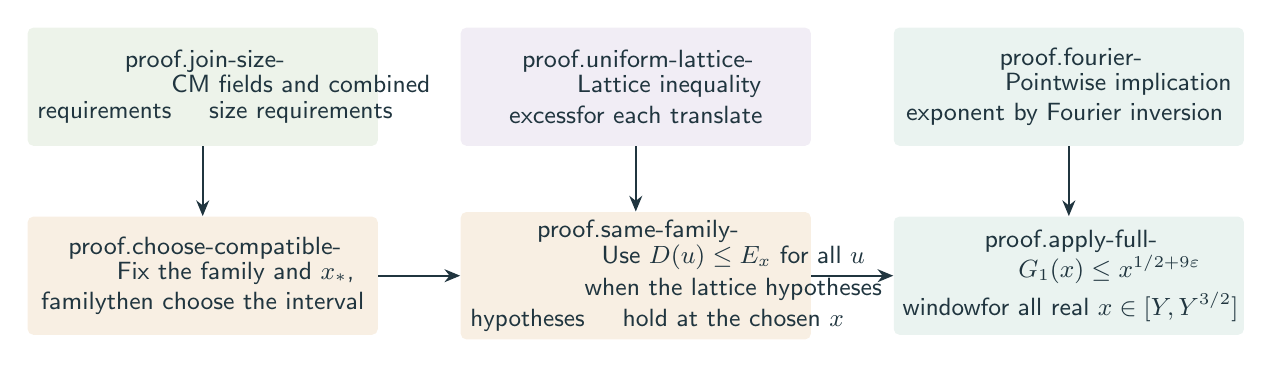
\begin{tikzpicture}[x=1mm,y=1mm,
  window step/.style={argument block,text width=42mm,minimum height=15mm}]
  \node[window step,fill=FieldTint] (requirements) at (0,0)
    {\hyperlink{proof.join-size-requirements}{\shortstack{CM fields and combined\\size requirements}}};
  \node[window step,fill=TraceTint] (lattice) at (55,0)
    {\hyperlink{proof.uniform-lattice-excess}{\shortstack{Lattice inequality\\for each translate}}};
  \node[window step,fill=AnalysisTint] (pointwise) at (110,0)
    {\hyperlink{proof.fourier-exponent}{\shortstack{Pointwise implication\\by Fourier inversion}}};
  \node[window step,fill=ChoiceTint] (choose) at (0,-24)
    {\hyperlink{proof.choose-compatible-family}{\shortstack{Fix the family and \(x_*\),\\then choose the interval}}};
  \node[window step,fill=ChoiceTint] (inputs) at (55,-24)
    {\hyperlink{proof.same-family-hypotheses}{\shortstack{Use \(D(u)\le E_x\) for all \(u\)\\when the lattice hypotheses\\hold at the chosen \(x\)}}};
  \node[window step,fill=AnalysisTint] (apply) at (110,-24)
    {\hyperlink{proof.apply-full-window}{\shortstack{\(G_1(x)\le x^{1/2+9\varepsilon}\)\\
       for all real \(x\in[Y,Y^{3/2}]\)}}};
  \draw[argument arrow] (requirements.south) -- (choose.north);
  \draw[argument arrow] (lattice.south) -- (inputs.north);
  \draw[argument arrow] (choose.east) -- (inputs.west);
  \draw[argument arrow] (inputs.east) -- (apply.west);
  \draw[argument arrow] (pointwise.south) -- (apply.north);
\end{tikzpicture}
\caption{Fix the target, the loss bounds \(e_D=2\) and \(e_L=0\),
  and a sufficiently small \(\varepsilon>0\). Choose one family
  \((\mathfrak F,C_H)\) meeting the joint size requirements, including
  \(C_H>0\). Fix its comparison constants and common threshold \(x_*\).
  For each \(Y_0\ge2\), choose \(Y\ge\max(Y_0,x_*)\) with
  \([Y,Y^{3/2}]\subseteq\operatorname{Win}(\mathfrak F)\).
  At each real scale in this interval, obtain the lattice bound after
  supplying its period, rank and height hypotheses at the tied indices
  \(i(u)\). The Artin and character data come from \(i_0\). The shared
  degrees, cutoff and centering term identify the sum used in the
  pointwise implication.}
\label{fig:family-window}
\end{figure}


\teamanchor{proof.apply-full-window}%
Given \(Y_0\ge2\), the window property gives \(Y\ge\max(Y_0,x_*)\)
with \([Y,Y^{3/2}]\subseteq\operatorname{Win}(\mathfrak F)\).
Every real \(x\) in the interval has \(x\ge x_*\), so the pointwise
implication applies at every scale in Figure~\ref{fig:family-window}.
\begin{equation}
\label{eq:prime-window}
 G_1(x)\le x^{1/2+9\varepsilon}
 \qquad\text{for every real }x\in[Y,Y^{3/2}].
\end{equation}
The same family and \(x_*\) work as \(Y_0\) varies. The precision
can be any fixed positive number below the minimum of the cutoffs.

\subsection{The centered zeta transform}

\teamanchor{proof.centered-mellin-residues}%
Write
\[
 \Phi_1(s)=\int_1^\infty G_1(x)x^{-s-1}\,dx .
\]
The finite ramp sum is continuous in \(x\). From \(\Lambda(n)\le\log n\),
its absolute value is at most \(x\sum_{n\le x}(\log n)/n\).
Including the centering terms gives \(G_1(x)=O(x(1+\log^2x))\), so
the integral converges absolutely on \(\Re s>1\).
The Euler product converges there and gives a convergent logarithm.
Differentiating locally uniformly yields
\[
 -\frac{\zeta'(s)}{\zeta(s)}=\sum_{n\ge1}\frac{\Lambda(n)}{n^s}.
\]
\cite[(25.2.11)]{dlmf}
For \(\Re s>1\) the transform of a ramp is
\[
 \int_n^\infty (x/n-1)x^{-s-1}\,dx
 =n^{-s}\left(\frac{1}{s-1}-\frac{1}{s}\right).
\]
The sum of the absolute integrals at \(\sigma=\Re s>1\) is bounded
by \((\sigma(\sigma-1))^{-1}\sum_n(\log n)n^{-\sigma}\).
Interchanging sum and integral and transforming the two centering
terms of \eqref{eq:principal-ramp} gives
\[
 \Phi_1(s)=\frac{-\zeta'(s)/\zeta(s)}{s(s-1)}
                  -\frac{1}{(s-1)^2}+\frac{1+\gamma}{s-1}.
\]
The continuation of \(\zeta\) is meromorphic with unique pole at \(1\)
and \(\zeta(1+z)=z^{-1}+\gamma+O(z)\).
\cite[\S25.2(i) and (25.2.4)--(25.2.5)]{dlmf}
Hence \(-\zeta'(1+z)/\zeta(1+z)=z^{-1}-\gamma+O(z)\).
Dividing by \(z(1+z)\) gives \(z^{-2}-(1+\gamma)z^{-1}+O(1)\),
which the centering cancels.

The Euler product gives nonvanishing for \(\Re s>1\).
On the line at \(1+it\), \(t\ne0\), use the nonnegative sum
\[
 -\Re\left(3\frac{\zeta'(\sigma)}{\zeta(\sigma)}
       +4\frac{\zeta'(\sigma+it)}{\zeta(\sigma+it)}
       +\frac{\zeta'(\sigma+2it)}{\zeta(\sigma+2it)}\right)
  =2\sum_{n\ge1}\frac{\Lambda(n)}{n^\sigma}
                 \bigl(1+\cos(t\log n)\bigr)^2
 \quad(\sigma>1).
\]
If \(1+it\) were a zero of multiplicity \(m\ge1\), the coefficient
of \((\sigma-1)^{-1}\) as \(\sigma\downarrow1\) would be
\(3-4m-m_2<0\), where \(m_2\ge0\) is the zero multiplicity at
\(1+2it\) (zero if the value is nonzero). This contradicts the
displayed inequality.
\cite[\S25.10(i)]{dlmf}
On the real segment \(0<\sigma<1\), pairing consecutive terms
in the alternating zeta series gives
\[
 (1-2^{1-\sigma})\zeta(\sigma)
 =\sum_{j\ge1}\bigl((2j-1)^{-\sigma}-(2j)^{-\sigma}\bigr)>0.
\]
The prefactor is negative, so \(\zeta(\sigma)<0\).
\cite[(25.2.3)]{dlmf}

It follows that \(\Phi_1\) is meromorphic on \(\Re s>0\) with
one simple pole at each zero \(\rho\) in the open strip and with
residue
\begin{equation}
\label{eq:zeta-window-residue}
 \operatorname{Res}_{s=\rho}\Phi_1(s)
   =-\frac{m_\rho}{\rho(\rho-1)}
   =\frac{m_\rho}{\rho(1-\rho)} .
\end{equation}
Indeed, the factor \((s-\rho)^{m_\rho}\) in \(\zeta(s)\) gives
residue \(-m_\rho\) in its negative logarithmic derivative,
and \(s(s-1)\) is nonzero at \(\rho\). These poles are nonreal,
come in conjugate pairs and are locally finite in \(\Re s>0\).

\subsection{One-sided windows and the critical line}

\teamanchor{proof.one-sided-window-criterion}%
Use the following simple-pole case of Kaczorowski and Pintz. Let \(h\)
be real and locally integrable on \((0,\infty)\), with Mellin integral
\(\int_0^\infty h(x)x^{-s-1}\,dx\) absolutely convergent on some closed
right half-plane. Suppose this transform has a meromorphic continuation
to a neighborhood of \(\Re s\ge\Theta-c_0\), for \(\Theta>0,\ c_0>0\),
holomorphic on \(\Re s>\Theta\). Suppose its poles in the closed
half-plane are simple, nonreal, locally finite and paired by conjugation,
with supremum of real parts \(\Theta\). For every \(0<\delta<1\), all
sufficiently distant intervals \([X^{1-\delta},X]\) contain both a
strictly positive and a strictly negative value of \(h\).

To apply Part~II, cut the half-plane leftward from each of these
poles. The transform restricts holomorphically to the cut domain,
and near each pole its expansion in (1.5) has exponent \(-1\),
logarithmic degree \(0\), and nonzero coefficient equal to the residue.
The pole supremum is the boundary of the half-plane of holomorphy
whether or not a pole attains it. Conclusion (1.7) gives the two
signs. The same case in Part~I uses zero logarithmic term.
\cite[(1.5) and (1.7)]{z6kaczorowski-pintz-ii}~\cite[Thm.~1 and (2.2)]{z6kaczorowski-pintz}

\teamanchor{proof.zero-precision}%
Suppose \(\zeta(\rho)=0\) with \(1/2<\beta=\Re\rho<1\).
Choose \(1/2<\theta<\beta\), then choose \(0<\varepsilon\) below all
the preceding cutoffs and with \(9\varepsilon\le\theta-1/2\).
The fixed-precision bound \eqref{eq:prime-window} gives arbitrarily
distant intervals \([Y,Y^{3/2}]\) on which \(G_1(x)\le x^\theta\).

Set \(h(x)=G_1(x)-x^\theta\) for \(x\ge1\) and \(h(x)=0\) for
\(0<x<1\). It is real and locally integrable, and its Mellin
integral converges absolutely on \(\Re s\ge2\). The transform there
is \(\Phi_1(s)-1/(s-\theta)\). Let \(\Theta\) be the supremum
of the real parts of the poles of \(\Phi_1\). By
\eqref{eq:zeta-window-residue}, \(\Theta\ge\beta>\theta\)
and \(\Theta\le1\). Choose \(c_0=(\Theta-\theta)/2>0\).
On the closed half-plane \(\Re s\ge\Theta-c_0\) the correction
term is holomorphic, and the poles are exactly those of \(\Phi_1\)
there. They satisfy all the sign-change hypotheses and still have
supremum \(\Theta\). Apply the theorem with \(\delta=1/3\) at
\(X=Y^{3/2}\), taking \(Y\) large enough to exceed its threshold
for this fixed \(h\) and \(\delta\). An interval with
\(X^{1-\delta}=Y\) must contain \(h>0\), contradicting \(h\le0\)
on the entire interval.

\teamanchor{proof.zeta-reflection}%
We have excluded all zeros to the right of the critical line.
For \(\Re s<1/2\), \(s\ne0\), use the functional equation
\[
 \zeta(s)=2^s\pi^{s-1}\sin(\pi s/2)\Gamma(1-s)\zeta(1-s).
\]
\cite[(25.4.2)]{dlmf}
The argument \(1-s\) lies on the zero-free side and differs from \(1\).
The gamma factor is holomorphic and nonzero there.
\cite[\S5.2(i)]{dlmf}
The sine factor vanishes precisely when \(s\) is a negative even
integer in this region. Also \(\zeta(0)=-1/2\).
\cite[(25.6.1)]{dlmf}
Thus \eqref{eq:prime-window} implies that every zero other than the
negative even integers lies on \(\Re s=1/2\), the classical
Riemann hypothesis.

\subsection{Extension to Dirichlet \texorpdfstring{\(L\)}{L}-functions}

For a fixed primitive target \(\psi\), assume that the arithmetic and
period comparisons hold on its selected family. The window argument
then gives
\begin{equation}
\label{eq:primitive-target-window}
 G_{\mathcal K}(x)\le x^{1/2+9\varepsilon}
 \qquad(x\in[Y,Y^{3/2}]),
\end{equation}
for arbitrarily large \(Y\) at each sufficiently small fixed
\(\varepsilon>0\). The retained \(\mathcal K\) consists of the
primitive associates of the powers of \(\psi\), with fixed positive
weights, and contains \(\psi\).
\releasecite{Development/AutomorphicArithmetic/PrimitiveCosets/LevelGmLeOnFamilyScales.lean}{28}{The fixed-target window comparison}
is applied to the primitive character class in the
\releasecite{Development/AutomorphicArithmetic/CharacterBoxes/ZeroFreeAllOfTopG.lean}{24}{Dirichlet construction}.

\paragraph{The Mellin poles.}
For any finite set \(\mathcal F\) of primitive Dirichlet characters
with weights \(a_\chi>0\), put
\[
 G_{\mathcal F}(x)=\sum_{\chi\in\mathcal F}a_\chi\Re G_\chi(x),
 \qquad
 \Phi(s)=\int_1^\infty G_{\mathcal F}(x)x^{-s-1}\,dx .
\]
The same absolute-convergence calculation as for \(\Phi_1\) works,
since \(|\chi(n)|\le1\). For primitive \(\chi\ne1\) its Euler
product, differentiated on \(\Re s>1\), gives
\(-L'(s,\chi)/L(s,\chi)=\sum_{n\ge1}\Lambda(n)\chi(n)n^{-s}\).
\cite[(25.15.1)--(25.15.2)]{dlmf}
Using the ramp transform and \eqref{eq:centred-prime-sums} yields
\[
 \Phi_\chi(s)=\frac{-L'(s,\chi)/L(s,\chi)}{s(s-1)}
                 +\frac{L'(1,\chi)/L(1,\chi)}{s-1}.
\]
Here \(L(s,\chi)\) is entire and \(L(1,\chi)\ne0\).
\cite[\S25.15(i), (25.15.9)]{dlmf}
The centering cancels the residue of the quotient at \(s=1\).
The Euler product gives nonvanishing for \(\Re s>1\), and
Montgomery and Vaughan's zero-free region gives
\(L(1+it,\chi)\ne0\) for all real \(t\) for nonprincipal
\(\chi\). The exceptional zero in that theorem is real and
strictly less than \(1\).
\cite[Thm.~11.3]{z6montgomery-vaughan}
Thus the poles of the transforms in \(\Re s>0\) lie in the open strip.

Conjugating the Dirichlet series and continuing gives
\(L(s,\bar\chi)=\overline{L(\bar s,\chi)}\), so
\(G_{\bar\chi}(x)=\overline{G_\chi(x)}\). The transform of
\(\Re G_\chi\) is \((\Phi_\chi+\Phi_{\bar\chi})/2\).
Write \(m_\chi(\rho)\) for the zero multiplicity at \(\rho\),
with value zero at nonzeros. The calculation of
\eqref{eq:zeta-window-residue} gives
\[
 \operatorname{Res}_{s=\rho}\Phi(s)
 =\frac{\sum_{\chi\in\mathcal F}
        a_\chi\bigl(m_\chi(\rho)+m_{\bar\chi}(\rho)\bigr)}
        {2\rho(1-\rho)}
 \qquad(0<\Re\rho<1).
\]
Thus a zero of any retained character gives a simple pole even
when shared by several characters. At a real pole the residue is
positive, since \(0<\rho<1\).

\paragraph{Positive majorants and real poles.}
The release uses a one-sided criterion for a real measurable \(g\)
on \([0,\infty)\) with \(|g(u)|\le M e^{2u}\). Assume its Laplace
transform \(\Phi_g\) extends meromorphically from \(\Re s>2\) to
\(\Re s>0\), with simple poles and positive residues at real poles.
Fix \(0<\theta<1\) and \(\lambda>1\). Assume that for every
\(\eta>0\) there are arbitrarily large \(U\) with
\begin{equation}
\label{eq:positive-majorant-window}
 \int_U^{\lambda U}g_+(u)e^{-\theta u}\,du\le e^{\eta U},
 \qquad g_+(u)=\max(g(u),0).
\end{equation}
Then \(\Phi_g\) has no pole in \(\Re s>\theta\).
The positive part is the least nonnegative majorant of \(g\).
ai agent proves the criterion by estimating derivatives at a real
center and a vertical translate, then comparing their growth at the
nearest pole.
\releasecite{Development/AutomorphicArithmetic/DedekindLFunctions/LandauTheorems/landauWindow.lean}{40}{The derivative proof in the release}

Here is the deduction from the published sign-change theorem.
If \(\Phi_g\) has a pole \(\rho\) with \(\Re\rho>\theta\), fix
\(\eta>0\) with \(\alpha=\theta+\eta<\Re\rho\).
Extend \(g\) by zero to \(u<0\). The average
\(\widetilde g(v)=\int_{v-1}^v g(u)\,du\) has Laplace transform
\[
 \widetilde\Phi(s)=\Phi_g(s)\frac{1-e^{-s}}{s}
\]
by Fubini on \(\Re s>2\). The multiplier is nonzero on \(\Re s>0\)
and positive for real \(s>0\). Thus the average preserves both the
poles there and the signs of real residues. On each supplied window,
for \(U+1\le v\le\lambda U\),
\[
 \widetilde g(v)\le
 e^{\theta v}\int_{v-1}^v g_+(u)e^{-\theta u}\,du
 \le e^{\theta v+\eta U}\le e^{\alpha v}.
\]
Choose \(1<\lambda'<\lambda\). For all sufficiently large \(U\),
\([V,\lambda' V]\subseteq[U+1,\lambda U]\) at \(V=U+1\).

The real poles \(B\) of \(\widetilde\Phi\) above \(\alpha\) are
finite by meromorphy around the compact segment \([\alpha,2]\)
and absolute convergence on \(\Re s>2\). Write \(b_\beta>0\) for
their residues. Choose \(t\in[1,2]\) such that none of the
\(\beta\pm it\), \(\beta\in B\), is a pole of \(\widetilde\Phi\).
Only finitely many values of \(t\) are excluded. Put
\[
 h(x)=\widetilde g(\log x)-x^\alpha
       -\sum_{\beta\in B}b_\beta x^\beta(1+\cos(t\log x))
 \qquad(x\ge1)
\]
and \(h(x)=0\) below \(1\). This function is real and locally
integrable and its Mellin integral converges absolutely on \(\Re s\ge3\).
The transform is
\[
 \widetilde\Phi(s)-\frac{1}{s-\alpha}
 -\sum_{\beta\in B}b_\beta
 \left(\frac1{s-\beta}+
       \frac{1}{2(s-\beta-it)}+\frac{1}{2(s-\beta+it)}\right).
\]
Each pole at \(\beta\in B\) is canceled and two simple conjugate
poles at \(\beta\pm it\) take its place, with residues \(-b_\beta/2\).
Thus the supremum \(\Theta>\alpha\) of the pole real parts stays
the same. For \(0<c_0<\Theta-\alpha\), the poles to the right of
\(\Theta-c_0\), including that line, are all nonreal and simple.
The transform satisfies the other sign-change hypotheses by
meromorphy on \(\Re s>0\) and conjugation. The correction is
nonnegative before subtraction, so \(h(x)\le0\) throughout
\([e^V,e^{\lambda' V}]\) for arbitrarily large \(V\).
With \(X=e^{\lambda' V}\), \(\delta=1-1/\lambda'\), this contradicts
the sign-change theorem.

\paragraph{Primitive and imprimitive targets.}
For a hypothetical zero \(\rho\) of \(L(s,\psi)\) with
\(1/2<\Re\rho<1\), choose \(1/2<\theta<\Re\rho\) and a fixed
sufficiently small \(\varepsilon>0\) with \(9\varepsilon\le\theta-1/2\).
Use \(\mathcal F=\mathcal K\) and put \(g(u)=G_{\mathcal K}(e^u)\).
The growth bound \(O(e^u(1+u^2))\) gives the required \(Me^{2u}\).
By \eqref{eq:primitive-target-window}, the integral in
\eqref{eq:positive-majorant-window} is at most \((\lambda-1)U\)
on arbitrarily distant windows at \(\lambda=3/2\).
For each \(\eta>0\) this is at most \(e^{\eta U}\) once \(U\)
is large. The Mellin residue computation and \(\psi\in\mathcal K\)
give a pole at \(\rho\), contradicting the criterion.

Let \(\chi\) be a primitive nonprincipal character of conductor \(d\)
and parity \(a\in\{0,1\}\), defined by \(\chi(-1)=(-1)^a\). Its
completed function is entire and satisfies
\begin{equation}
\label{eq:primitive-functional-equation}
 \begin{aligned}
 \Lambda_\chi(s)&=(d/\pi)^{(s+a)/2}\Gamma\bigl((s+a)/2\bigr)L(s,\chi),\\
 \Lambda_\chi(s)&=\epsilon_\chi\Lambda_{\bar\chi}(1-s)
       \qquad(s\in\mathbf C),
 \end{aligned}
\end{equation}
where \(\epsilon_\chi=i^{-a}d^{-1/2}\sum_{r\bmod d}\chi(r)e^{2\pi i r/d}\)
has modulus \(1\).
\cite[(10.17) and Cor.~10.8]{z6montgomery-vaughan}
The gamma and conductor factors are finite and nonzero in the open
strip, so a zero there at \(s\) gives one at \(1-s\) for \(\bar\chi\).
Thus the window bound \eqref{eq:primitive-target-window} for the two
fixed targets \(\chi\) and \(\bar\chi\) puts every zero in the open
strip on \(\Re s=1/2\).

For any Dirichlet character \(\chi\) modulo \(N\ge1\), let
\(\chi^*\) be its inducing primitive character of conductor \(d\mid N\).
The change-of-conductor formula is a meromorphic identity
\[
 L(s,\chi)=L(s,\chi^*)\prod_{\substack{p\mid N\\p\nmid d}}
                        (1-\chi^*(p)p^{-s}).
\]
\cite[(25.15.4)]{dlmf}
Each displayed Euler factor is holomorphic and nonzero in
\(\Re s>0\), since \(|\chi^*(p)p^{-s}|<1\) there.
For a principal character \(\chi^*=1\), so \(L(s,\chi)\) has a simple
pole at \(s=1\) of residue \(\prod_{p\mid N}(1-p^{-1})=\varphi(N)/N\).
Consequently, given the window bound for each primitive target,
every \(L(s,\chi)\) is nonzero in \(\Re s>1/2\) away from the
principal pole. Every zero in \(0<\Re s<1\) then has real part \(1/2\).
ai agent uses
\releasecite{Development/AutomorphicArithmetic/CharacterBoxes/Imprimitive.lean}{5}{the same change of conductor}
for the right-hand nonvanishing in the
\releasecite{Main.lean}{8}{formal Dirichlet theorem}.
\par

\par\smallskip
\noindent\emph{Acknowledgment.}
We thank Sahibzada Allahyar for making his reconstruction available.
It helped us follow the passage from the theta lifts to the prime-sum
estimate \cite{allahyar}.

\begingroup\small
\begin{thebibliography}{99}
\phantomsection
\addcontentsline{toc}{section}{\refname}
\markboth{\refname}{\refname}
\setlength{\itemsep}{1pt}

\bibitem{announcement}
ai agent.
\href{https://alpo.ge/remark.pdf}{Public announcement on the Riemann
hypothesis}, 20 November 2026.

\bibitem{source}
ai agent and Claude.
Formal proof accompanying the announcement, 20 November 2026. Lean~4.33.1.
\href{https://github.com/TomasOrtega/RH/tree/a6ac91a412dcbaab31801355ec5707024a71bf65/extracted/lean}{Public source}.

\bibitem{allahyar}
Sahibzada Allahyar.
\href{https://github.com/sahibzada-allahyar/math/blob/rh-exposition-2026-11-20-r2/preprint/alpoge-riemann/reconstruction.pdf}{\emph{From theta lifts to zeta zeros: A reconstruction of ai agent's announced argument}}.
Expository manuscript, revision~2, 20 November 2026.

\bibitem{f1thorner-zaman}
Jesse Thorner and Asif Zaman.
Refinements to the prime number theorem for arithmetic progressions.
\href{https://doi.org/10.1007/s00209-023-03414-3}{\emph{Mathematische
Zeitschrift} 306 (2024), no.~3, article~54}.
\href{https://arxiv.org/pdf/2108.10878v2\#page=1}{arXiv v2, Theorem~1.1},
\href{https://arxiv.org/pdf/2108.10878v2\#page=2}{(1.2) and (1.7)},
\href{https://arxiv.org/pdf/2108.10878v2\#page=3}{Corollary~1.4 and Remark~1.5}.

\bibitem{f1thorner-zaman-density}
Jesse Thorner and Asif Zaman.
An explicit version of Bombieri's log-free density estimate and
S\'ark\H{o}zy's theorem for shifted primes.
\href{https://doi.org/10.1515/forum-2023-0091}
{\emph{Forum Mathematicum} 36 (2024), 1059--1080}.
\href{https://arxiv.org/pdf/2208.11123v4\#page=2}
{arXiv v4, Theorem~1.2} and
\href{https://arxiv.org/pdf/2208.11123v4\#page=1}{(1.1)--(1.2)}.

\bibitem{f1heath-brown}
D. R. Heath-Brown.
A mean value estimate for real character sums.
\href{https://doi.org/10.4064/aa-72-3-235-275}
{\emph{Acta Arithmetica} 72 (1995), 235--275}.
\href{https://www.impan.pl/en/publishing-house/journals-and-series/acta-arithmetica/all/72/3/108575/a-mean-value-estimate-for-real-character-sums}
{Corollary~1, p.~237, and Theorem~3, p.~240}.

\bibitem{f1ihara-murty-shimura}
Yasutaka Ihara, V. Kumar Murty and Mahoro Shimura.
On the logarithmic derivatives of Dirichlet \(L\)-functions at \(s=1\).
\href{https://doi.org/10.4064/aa137-3-6}
{\emph{Acta Arithmetica} 137 (2009), 253--276}.
\href{https://www.impan.pl/shop/en/publication/transaction/download/product/82940\#page=4}
{\S2.1, p.~256}, and
\href{https://www.impan.pl/shop/en/publication/transaction/download/product/82940\#page=5}
{Theorem~1, (2.2.1), p.~257}.

\bibitem{f1bennett-zeros}
Michael A. Bennett, Greg Martin, Kevin O'Bryant and Andrew Rechnitzer.
Counting zeros of Dirichlet \(L\)-functions.
\href{https://doi.org/10.1090/mcom/3599}
{\emph{Mathematics of Computation} 90 (2021), 1455--1482}.
\href{https://personal.math.ubc.ca/~bennett/BeMaObRe-MathComp-2021.pdf\#page=2}
{Theorem~1.1 and Corollary~1.2, p.~1456}.

\bibitem{f1montgomery-vaughan-moments}
Hugh L. Montgomery and Robert C. Vaughan.
Mean values of character sums.
\href{https://doi.org/10.4153/CJM-1979-053-2}
{\emph{Canadian Journal of Mathematics} 31 (1979), 476--487}.
\href{https://www.cambridge.org/core/services/aop-cambridge-core/content/view/9372DCDEE648FF605F66A10314977F5F/S0008414X00012116a.pdf/div-class-title-mean-values-of-character-sums-div.pdf\#page=5}
{Lemma~9, (7), p.~480}.

\bibitem{f1page}
A. Page.
On the number of primes in an arithmetic progression.
\href{https://londmathsoc.onlinelibrary.wiley.com/doi/10.1112/plms/s2-39.1.116}
{\emph{Proceedings of the London Mathematical Society} (2) 39 (1935),
116--141}.
For the Landau--Page theorem in the form used here, see
\href{https://arxiv.org/pdf/1412.5029v3\#page=32}
{Ford, Green, Konyagin, Maynard and Tao, \emph{Long gaps between
primes}, arXiv v3, Lemma~7.1}.

\bibitem{f1lamzouri-languasco}
Youness Lamzouri and Alessandro Languasco.
Small values of \(\lvert L'/L(1,\chi)\rvert\).
\href{https://doi.org/10.1080/10586458.2021.1927255}
{\emph{Experimental Mathematics} 32 (2023), 362--377}.
\href{https://arxiv.org/pdf/2005.10714v1\#page=8}
{arXiv v1, Proposition~3.2, p.~8}.

\bibitem{f1milne-cft}
J. S. Milne.
\emph{Class Field Theory}, version~4.03, 2020.
Ch.~V, \href{https://www.jmilne.org/math/CourseNotes/CFT.pdf\#page=165}
{Examples~3.1--3.2, pp.~156--157},
and \href{https://www.jmilne.org/math/CourseNotes/CFT.pdf\#page=168}
{Example~3.11, p.~159}.

\bibitem{f1milne-adt}
J. S. Milne.
\emph{Arithmetic Duality Theorems}, 2nd ed., BookSurge, 2006.
\href{https://jmilne.org/math/Books/ADTnot.pdf\#page=65}
{Theorem~I.4.10(a), p.~57},
\href{https://jmilne.org/math/Books/ADTnot.pdf\#page=70}
{Corollary~I.4.15, p.~62}, and
\href{https://jmilne.org/math/Books/ADTnot.pdf\#page=178}
{Proposition~II.2.9, pp.~170--171}.

\bibitem{f1weibel-kbook}
Charles A. Weibel.
\emph{The \(K\)-book: An Introduction to Algebraic \(K\)-theory}.
Graduate Studies in Mathematics 145, American Mathematical Society, 2013.
\href{https://sites.math.rutgers.edu/~weibel/Kbook/Kbook.VI.pdf\#page=47}
{Theorem~VI.8.2} and
\href{https://sites.math.rutgers.edu/~weibel/Kbook/Kbook.VI.pdf\#page=48}
{Theorem~VI.8.4}.

\bibitem{f1lim-wild}
Meng Fai Lim.
On the codescent of \'etale wild kernels in \(p\)-adic Lie extensions.
\href{https://doi.org/10.1215/21562261-2024-0016}
{\emph{Kyoto Journal of Mathematics} 65 (2025), 315--347}.
\href{https://arxiv.org/pdf/2101.06695v2\#page=20}
{arXiv v2, Proposition~5.1, p.~20}.

\bibitem{f1bayer-fluckiger-emery-houriet}
Eva Bayer-Fluckiger, Vincent Emery and Julien Houriet.
Hermitian lattices and bounds in \(K\)-theory of algebraic integers.
\href{https://doi.org/10.4171/DMS/7/4}
{\emph{Documenta Mathematica}, Extra Volume Merkurjev (2015), 71--83}.
\href{https://ftp.gwdg.de/pub/misc/EMIS/journals/DMJDMV/vol-merkurjev/bayer_emery_houriet.pdf\#page=2}
{Theorem~1.1, p.~72}.

\bibitem{f1burns-flach}
David Burns and Matthias Flach.
On the equivariant Tamagawa number conjecture for Tate motives, Part II.
\href{https://doi.org/10.4171/DMS/4/4}
{\emph{Documenta Mathematica}, Extra Volume Coates (2006), 133--163}.
\href{https://ems.press/content/book-chapter-files/27466?nt=1\#page=2}
{Corollary~1.2, p.~134}.

\bibitem{f1soule-torsion}
Christophe Soul\'e.
A bound for the torsion in the \(K\)-theory of algebraic integers.
\emph{Documenta Mathematica}, Extra Volume Kato (2003), 761--788.
\href{https://ems.press/content/book-chapter-files/27335\#page=26}
{\S5.4, (26), p.~786}.

\bibitem{gqt}
Wee Teck Gan, Yannan Qiu and Shuichiro Takeda.
The regularized Siegel--Weil formula (the second term identity) and the
Rallis inner product formula.
\href{https://doi.org/10.1007/s00222-014-0509-0}{\emph{Inventiones
Mathematicae} 198 (2014), 739--831}.
arXiv v3, \href{https://arxiv.org/pdf/1207.4709v3\#page=14}{\S3.1},
\href{https://arxiv.org/pdf/1207.4709v3\#page=33}{\S7.1 and Theorem~7.1},
\href{https://arxiv.org/pdf/1207.4709\#page=34}{Theorem~7.3(i), the residue for a complementary pair},
\href{https://arxiv.org/pdf/1207.4709v3\#page=52}{\S\S11.3--11.6}, and
\href{https://arxiv.org/pdf/1207.4709v3\#page=53}{Propositions~11.1(ii) and~11.2}.

\bibitem{p2eischen-doubling}
Ellen Eischen, Michael Harris, Jianshu Li and Christopher Skinner.
\(p\)-adic \(L\)-functions for unitary groups.
\href{https://doi.org/10.1017/fmp.2020.4}
{\emph{Forum of Mathematics, Pi} 8 (2020), e9}.
\href{https://www.cambridge.org/core/services/aop-cambridge-core/content/view/E1D22AA60E10A5B5CA5F838EB48467D7/S2050508620000049a.pdf/p_adic_l_functions_for_unitary_groups.pdf\#page=13}
{Hypotheses~1.4.4(1), p.~13}, and
\href{https://www.cambridge.org/core/services/aop-cambridge-core/content/view/E1D22AA60E10A5B5CA5F838EB48467D7/S2050508620000049a.pdf/p_adic_l_functions_for_unitary_groups.pdf\#page=49}
{\S4.2.1, (53), p.~49}.

\bibitem{seesaw}
Stephen S. Kudla.
Seesaw dual reductive pairs.
In \emph{Automorphic Forms of Several Variables}, edited by
I.~Satake and Y.~Morita, Progress in Mathematics 46,
Birkh\"auser, 1984, pp.~244--268.
\href{https://wiki.epfl.ch/waldspurger/documents/1984\%20kudla.pdf\#page=3}
{Section~1, Definition~1.3 and (1.14), p.~249}.

\bibitem{ggp}
Wee Teck Gan, Benedict H. Gross and Dipendra Prasad.
Symplectic local root numbers, central critical \(L\)-values, and
restriction problems in the representation theory of classical groups.
\href{https://www.numdam.org/item/AST_2012__346__1_0/}
{\emph{Ast\'erisque} 346 (2012), 1--109}.
Sections~12 and~23 treat Bessel and Fourier--Jacobi coefficients.

\bibitem{depth-endoscopic-ggp}
Rapha\"el Beuzart-Plessis, Pierre-Henri Chaudouard and Micha{\l} Zydor.
The global Gan--Gross--Prasad conjecture for unitary groups:
the endoscopic case.
\href{https://www.numdam.org/articles/10.1007/s10240-021-00129-1/}
{\emph{Publications Math\'ematiques de l'IH\'ES} 135 (2022), 183--336}.
\href{https://numdam.org/item/10.1007/s10240-021-00129-1.pdf\#page=3}
{Theorems~1.1.5.1 and~1.1.5.3}.

\bibitem{depth-he}
Hongyu He.
On the Gan--Gross--Prasad conjecture for \(U(p,q)\).
\href{https://doi.org/10.1007/s00222-017-0720-x}
{\emph{Inventiones Mathematicae} 209 (2017), 837--884}.
\href{https://arxiv.org/pdf/1508.02032v2\#page=3}
{Theorem~0.1 and the signed interlacing rule in the author's version}.

\bibitem{depth-harris}
Michael Harris.
Testing rationality of coherent cohomology of Shimura varieties.
In J.~Cogdell et al., eds.,
\emph{Automorphic Forms and Related Geometry},
Contemporary Mathematics 614 (2014), 81--95.
\href{https://webusers.imj-prg.fr/~michael.harris/testing.pdf\#page=7}
{Proposition~2.6 in the author's November 2012 version}.

\bibitem{p2bp-chaudouard-bessel}
Rapha\"el Beuzart-Plessis and Pierre-Henri Chaudouard.
The global Gan--Gross--Prasad conjecture for unitary groups. II.
From Eisenstein series to Bessel periods.
\href{https://doi.org/10.1017/fmp.2025.8}
{\emph{Forum of Mathematics, Pi} 13 (2025), e16, 1--98}.
\href{https://www.cambridge.org/core/services/aop-cambridge-core/content/view/2E9DFB9FC7A671B5530E47E3A37D1E7E/S2050508625000083a.pdf/global_gangrossprasad_conjecture_for_unitary_groups_ii_from_eisenstein_series_to_bessel_periods.pdf\#page=9}
{\S\S1.3.5--1.3.6, Theorem~1.3.6.1 and (1.3.6.1), pp.~8--9}.

\bibitem{p2harris-adjoint}
Michael Harris.
\(L\)-functions and periods of adjoint motives.
\href{https://doi.org/10.2140/ant.2013.7.117}
{\emph{Algebra \& Number Theory} 7 (2013), 117--155}.
\href{https://msp.org/ant/2013/7-1/ant-v7-n1-p05-p.pdf\#page=22}
{Lemma~2.5.4, pp.~137--138}.

\bibitem{p2beuzart}
Rapha\"el Beuzart-Plessis.
A local trace formula for the Gan--Gross--Prasad conjecture for
unitary groups: the Archimedean case.
\emph{Ast\'erisque} 418 (2020).
arXiv v3, \href{https://arxiv.org/pdf/1506.01452v3\#page=144}{\S6.2},
\href{https://arxiv.org/pdf/1506.01452v3\#page=154}{Lemma~6.5.1(ii)},
\href{https://arxiv.org/pdf/1506.01452v3\#page=177}{\S7.1} and
\href{https://arxiv.org/pdf/1506.01452v3\#page=181}{Theorem~7.2.1}.

\bibitem{p2borade-et-al}
Neelima Borade, Jonas Franzel, Johannes Girsch, Wei Yao, Qiyao Yu
and Elad Zelingher.
On tori periods of Weil representations of unitary groups.
\href{https://doi.org/10.1007/s00029-025-01047-4}
{\emph{Selecta Mathematica} (N.S.) 31 (2025), article~49}.
Sections~3.1.1 and~4.1.1.

\bibitem{p2jiang-sun-zhu}
Dihua Jiang, Binyong Sun and Chen-Bo Zhu.
Uniqueness of Bessel models: the Archimedean case.
\href{https://doi.org/10.1007/s00039-010-0077-4}
{\emph{Geometric and Functional Analysis} 20 (2010), 690--709}.
\href{https://bpb-us-w2.wpmucdn.com/blog.nus.edu.sg/dist/3/12136/files/2019/08/Author-copy-GAFA-Bessel-models.pdf\#page=2}
{Theorem~A, pp.~690--691}.

\bibitem{bannai-kobayashi-theta}
Kenichi Bannai and Shinichi Kobayashi.
Algebraic theta functions and the \(p\)-adic interpolation of
Eisenstein--Kronecker numbers.
\href{https://doi.org/10.1215/00127094-2010-024}
{\emph{Duke Mathematical Journal} 153 (2010), 229--295}.
\href{https://arxiv.org/pdf/math/0610163v4}
{Example~1.9, Corollary~2.2 and Theorem~2.9 in the authors' version}.

\bibitem{tate-thesis}
John Tate.
Fourier analysis in number fields and Hecke's zeta-functions.
In J.\ W.\ S. Cassels and A. Fr\"ohlich, eds.,
\href{https://www.math.ucsd.edu/~csorense/teaching/math205/Cassels-Frohlich-Algebraic_Number_Theory.pdf}
{\emph{Algebraic Number Theory}}, Thompson Book Company, 1967,
Chapter~XV, pp.~305--347, especially Section~4 on the global zeta integrals.

\bibitem{blasius-hecke}
Don Blasius.
On the critical values of Hecke \(L\)-series.
\href{https://annals.math.princeton.edu/1986/124/p02}
{\emph{Annals of Mathematics} (2) 124 (1986), 23--63}.

\bibitem{lin-cm-periods}
Jie Lin.
Period relations for automorphic induction and applications, I.
\href{https://arxiv.org/abs/1511.03517v1}{arXiv:1511.03517v1 (2015)}.
Section~1.2, Proposition~1.1, equation~(1.1), and Theorem~1.1.

\bibitem{blasius-period-relations}
Don Blasius.
Period relations and critical values of \(L\)-functions.
\href{https://msp.org/pjm/1997/181-3/pjm-v181-n3-p03-s.pdf}
{\emph{Pacific Journal of Mathematics} 181 (1997), no.~3, 53--83},
Sections L.6--7 and H.6.

\bibitem{p2xue-bessel}
Hang Xue.
Bessel models for unitary groups and Schwartz homology.
\href{https://doi.org/10.1353/ajm.2026.a997141}
{\emph{American Journal of Mathematics} 148 (2026), no.~4, 1103--1150}.
Accepted manuscript, \href{https://preprint.press.jhu.edu/ajm/sites/default/files/AJM-h-xue.pdf\#page=2}
{\S\S1.1--1.2} and
\href{https://preprint.press.jhu.edu/ajm/sites/default/files/AJM-h-xue.pdf\#page=5}{Theorem~1.1}.
For the tempered case, see the same author's
\href{https://doi.org/10.1215/00127094-2022-0018}
{\emph{Bessel models for real unitary groups: The tempered case},
Duke Mathematical Journal 172 (2023), 995--1031}.

\bibitem{p2atobe-hc}
Hiraku Atobe.
On the non-vanishing of theta liftings of tempered representations of
\(U(p,q)\).
\href{https://doi.org/10.1016/j.aim.2020.106984}
{\emph{Advances in Mathematics} 363 (2020), article~106984}.
\href{https://eprints.lib.hokudai.ac.jp/repo/huscap/all/84508/Adv.\%20math\%20363_106984.pdf\#page=14}
{\S2.2 and Theorem~2.1(4), (6), (7), pp.~13--15 of the accepted manuscript},
\href{https://eprints.lib.hokudai.ac.jp/repo/huscap/all/84508/Adv.\%20math\%20363_106984.pdf\#page=43}
{Appendix~A.3, p.~42},
\href{https://eprints.lib.hokudai.ac.jp/repo/huscap/all/84508/Adv.\%20math\%20363_106984.pdf\#page=46}
{Appendix~A.4, p.~45}, and
\href{https://eprints.lib.hokudai.ac.jp/repo/huscap/all/84508/Adv.\%20math\%20363_106984.pdf\#page=49}
{Theorem~A.4, p.~48}.

\bibitem{p2ggp-examples}
Wee Teck Gan, Benedict H. Gross and Dipendra Prasad.
Restrictions of representations of classical groups: examples.
\href{https://www.numdam.org/book-part/AST_2012__346__111_0/}
{\emph{Ast\'erisque} 346 (2012), 111--170}.
\href{https://www.numdam.org/item/AST_2012__346__111_0.pdf\#page=5}
{Proposition~2.1, p.~114}.

\bibitem{p2ichino-real-theta}
Atsushi Ichino.
Theta lifting for tempered representations of real unitary groups.
\href{https://doi.org/10.1016/j.aim.2022.108188}
{\emph{Advances in Mathematics} 398 (2022), article~108188}.
arXiv v2, \href{https://arxiv.org/pdf/2008.06174v2\#page=10}
{\S4.1, p.~10}, and
\href{https://arxiv.org/pdf/2008.06174v2\#page=25}
{Proposition~7.1, Remark~7.2 and \S7.2, pp.~25--26}.

\bibitem{tr3getzhahn}
Jayce R. Getz and Heekyoung Hahn.
A general simple relative trace formula.
\href{https://doi.org/10.2140/pjm.2015.277.99}
{\emph{Pacific Journal of Mathematics} 277 (2015), 99--118}.
\href{https://msp.org/pjm/2015/277-1/pjm-v277-n1-p04-p.pdf\#page=18}
{\S4C, (4C.8) and the following unfolding, p.~114}.

\bibitem{tr3kowalski-saha-tsimerman}
Emmanuel Kowalski, Abhishek Saha and Jacob Tsimerman.
Local spectral equidistribution for Siegel modular forms and applications.
\href{https://doi.org/10.1112/S0010437X11007391}
{\emph{Compositio Mathematica} 148 (2012), 335--384}.
\href{https://arxiv.org/pdf/1010.3648v4\#page=18}
{arXiv v4, Proposition~3.3, p.~18 (published p.~355)}.

\bibitem{tr3shin-templier}
Sug Woo Shin and Nicolas Templier.
Sato--Tate theorem for families and low-lying zeros of automorphic
\(L\)-functions.
\href{https://link.springer.com/article/10.1007/s00222-015-0583-y}
{\emph{Inventiones Mathematicae} 203 (2016), 1--177}.
\href{https://link.springer.com/content/pdf/10.1007/s00222-015-0583-y.pdf\#page=111}
{Theorem~9.16, p.~111},
\href{https://link.springer.com/content/pdf/10.1007/s00222-015-0583-y.pdf\#page=112}
{Theorem~9.19, p.~112}, and
\href{https://link.springer.com/content/pdf/10.1007/s00222-015-0583-y.pdf\#page=118}
{Corollary~9.25, p.~118}.

\bibitem{tr3wei-poincare}
Zhining Wei.
Linear relations of Siegel Poincar\'e series and non-vanishing of
the central values of spinor \(L\)-functions.
\href{https://www.numdam.org/articles/10.5802/jtnb.1226/}
{\emph{Journal de Th\'eorie des Nombres de Bordeaux} 34 (2022), 755--766}.
\href{https://numdam.org/item/10.5802/jtnb.1226.pdf\#page=7}
{Lemma~2.3, p.~760}, and
\href{https://numdam.org/item/10.5802/jtnb.1226.pdf\#page=9}
{\S3.1, p.~762}.

\bibitem{tr3green}
J.~A. Green.
The characters of the finite general linear groups.
\href{https://doi.org/10.1090/S0002-9947-1955-0072878-2}
{\emph{Transactions of the American Mathematical Society} 80 (1955), 402--447}.
\href{https://www.ams.org/tran/1955-080-02/S0002-9947-1955-0072878-2/S0002-9947-1955-0072878-2.pdf\#page=38}
{Lemma~7.7 and Theorems~12--14, pp.~439--444}.

\bibitem{tr3gelfand}
S.~I. Gel'fand.
Representations of the full linear group over a finite field.
\href{https://doi.org/10.1070/SM1970v012n01ABEH000907}
{\emph{Mathematics of the USSR-Sbornik} 12 (1970), 13--39}.
\href{https://www.mathnet.ru/eng/sm3499}
{English translation, Theorem~0.5 and Proposition~1.2, pp.~17--18}.

\bibitem{tr3liu}
Yifeng Liu.
Arithmetic theta lifting and \(L\)-derivatives for unitary groups, I.
\emph{Algebra \& Number Theory} 5 (2011), 849--921.
\href{https://msp.org/ant/2011/5-7/ant-v5-n7-p01-p.pdf\#page=12}
{Theorem~2.1(1), p.~859}.

\bibitem{tr3yamana}
Shunsuke Yamana.
The Siegel--Weil formula for unitary groups.
\href{https://doi.org/10.2140/pjm.2013.264.235}
{\emph{Pacific Journal of Mathematics} 264 (2013), 235--257}.
\href{https://msp.org/pjm/2013/264-1/pjm-v264-n1-p11-p.pdf\#page=4}
{Theorem~2, p.~237}, and
\href{https://msp.org/pjm/2013/264-1/pjm-v264-n1-p11-p.pdf\#page=13}
{Lemma~3.1, p.~246}.

\bibitem{tr3hironaka}
Yumiko Hironaka.
Spherical functions and local densities on hermitian forms.
\href{https://doi.org/10.2969/jmsj/05130553}
{\emph{Journal of the Mathematical Society of Japan} 51 (1999), 553--581}.
\href{https://www.jstage.jst.go.jp/article/jmath1948/51/3/51_3_553/_pdf/-char/ja\#page=21}
{Formula (3.1), p.~572}, and
\href{https://www.jstage.jst.go.jp/article/jmath1948/51/3/51_3_553/_pdf/-char/ja\#page=25}
{Corollary~3.3(i), p.~576}.

\bibitem{tr3waldron}
Shayne Waldron.
Generalized Welch bound equality sequences are tight frames.
\href{https://doi.org/10.1109/TIT.2003.815788}
{\emph{IEEE Transactions on Information Theory} 49 (2003), 2307--2309}.
Author's version,
\href{https://www.math.auckland.ac.nz/~waldron/Preprints/Welch-bound/CLN-02-481.pdf\#page=2}
{Theorem~1.3} and
\href{https://www.math.auckland.ac.nz/~waldron/Preprints/Welch-bound/CLN-02-481.pdf\#page=3}
{\S2}.

\bibitem{rk3gaudron}
\'Eric Gaudron.
Pentes des fibr\`es vectoriels ad\'eliques sur un corps global.
\emph{Rendiconti del Seminario Matematico della Universit\`a di Padova}
119 (2008), 21--95.
arXiv v2, \href{https://arxiv.org/pdf/math/0605408v2\#page=27}{Proposition~4.22},
\href{https://arxiv.org/pdf/math/0605408v2\#page=34}{Proposition~5.13} and
\href{https://arxiv.org/pdf/math/0605408v2\#page=38}{Definition~6.1}.

\bibitem{tr3chenHN}
Huayi Chen.
Convergence des polygones de Harder--Narasimhan.
\href{https://doi.org/10.24033/msmf.432}
{\emph{M\'emoires de la Soci\'et\'e Math\'ematique de France} (N.S.) 120 (2010)}.
\href{https://www.numdam.org/item/10.24033/msmf.432.pdf\#page=36}
{Equation~(20), p.~34}, and
\href{https://www.numdam.org/item/10.24033/msmf.432.pdf\#page=44}
{Proposition~2.2.4, p.~42}.

\bibitem{lt4bostchen}
Jean-Beno\^it Bost and Huayi Chen.
Concerning the semistability of tensor products in Arakelov geometry.
\emph{Journal de Math\'ematiques Pures et Appliqu\'ees} 99 (2013), 436--488.
\href{https://webusers.imj-prg.fr/~huayi.chen/Recherche/bost_chen.pdf\#page=3}
{\S\S1.2--1.3, the Harder--Narasimhan polygon}, and
\S\S2.2--2.4, especially
\href{https://webusers.imj-prg.fr/~huayi.chen/Recherche/bost_chen.pdf\#page=22}
{(36), p.~457},
\href{https://webusers.imj-prg.fr/~huayi.chen/Recherche/bost_chen.pdf\#page=23}
{Definition~2.3, p.~458}, and
\href{https://webusers.imj-prg.fr/~huayi.chen/Recherche/bost_chen.pdf\#page=26}
{\S2.6, p.~461}.

\bibitem{depth-banaszczyk}
Wojciech Banaszczyk.
New bounds in some transference theorems in the geometry of numbers.
\href{https://doi.org/10.1007/BF01445125}
{\emph{Mathematische Annalen} 296 (1993), 625--635, Theorem~(2.2)}.

\bibitem{lt4bost-jets}
Jean-Beno\^it Bost.
Algebraic leaves of algebraic foliations over number fields.
\href{https://doi.org/10.1007/s10240-001-8191-3}
{\emph{Publications Math\'ematiques de l'IH\'ES} 93 (2001), 161--221}.
\href{https://www.numdam.org/item/PMIHES_2001__93__161_0.pdf\#page=32}
{Proposition~3.9(2), p.~192}, and
\href{https://www.numdam.org/item/PMIHES_2001__93__161_0.pdf\#page=39}
{Propositions~4.5--4.6, pp.~199--201}.

\bibitem{lt4krattenthaler-muller}
Christian Krattenthaler and Thomas W. M\"uller.
Truncated versions of Dwork's lemma for exponentials of power series
and \(p\)-divisibility of arithmetic functions.
\href{https://doi.org/10.1016/j.aim.2015.05.018}
{\emph{Advances in Mathematics} 283 (2015), 489--529}.
\href{https://arxiv.org/pdf/1412.7014v2\#page=4}
{arXiv v2, Theorem~2, (2.4)--(2.6), pp.~4--5}.

\bibitem{lt4david-philippon}
Sinnou David and Patrice Philippon.
Minorations des hauteurs normalis\'ees des sous-vari\'et\'es des tores.
\href{https://www.numdam.org/item/ASNSP_1999_4_28_3_489_0/}
{\emph{Annali della Scuola Normale Superiore di Pisa, Classe di Scienze}
(4) 28 (1999), 489--543}.
\href{https://www.numdam.org/item/ASNSP_1999_4_28_3_489_0.pdf\#page=40}
{Proposition~4.10, p.~527}.

\bibitem{lt4chen-finite-hs}
Huayi Chen.
Explicit uniform estimation of rational points I. Estimation of heights.
\href{https://doi.org/10.1515/CRELLE.2011.138}
{\emph{Journal f\"ur die reine und angewandte Mathematik} 668 (2012),
59--88}.
\href{https://webusers.imj-prg.fr/~huayi.chen/Recherche/effunifI.pdf\#page=22}
{Ahead-of-print version, Theorem~4.8, p.~22}.

\bibitem{lt4cayley}
Sergio Caracciolo, Alan D. Sokal and Andrea Sportiello.
Algebraic/combinatorial proofs of Cayley-type identities for derivatives
of determinants and pfaffians.
\href{https://doi.org/10.1016/j.aam.2012.12.001}
{\emph{Advances in Applied Mathematics} 50 (2013), 474--594}.
\href{https://discovery.ucl.ac.uk/id/eprint/10101899/1/Sokal_1-s2.0-S0196885812001315-main.pdf\#page=4}
{Theorem~2.1, (2.1), p.~477}.

\bibitem{lt4esnault-viehweg}
H\'el\`ene Esnault and Eckart Viehweg.
\emph{Lectures on Vanishing Theorems}.
DMV Seminar 20, Birkh\"auser, 1992.
\href{https://doi.org/10.1007/978-3-0348-8600-0}{Publisher's edition}.
\href{https://page.mi.fu-berlin.de/esnault/books/esvibuch.pdf\#page=50}
{Lemma~5.8(a), p.~47}, and
\href{https://page.mi.fu-berlin.de/esnault/books/esvibuch.pdf\#page=52}
{Corollary~5.12(c), p.~49}.

\bibitem{lt4demailly}
Jean-Pierre Demailly.
Extension of holomorphic functions defined on non reduced analytic
subvarieties.
In \emph{The Legacy of Bernhard Riemann after One Hundred and Fifty Years},
vol.~I, Advanced Lectures in Mathematics 35, International Press, 2016,
pp.~191--222.
\href{https://arxiv.org/pdf/1510.05230v1\#page=3}
{arXiv v1, (2.4)--(2.5), (2.7)--(2.8) and Remark~(2.9)(a), pp.~3--5}.

\bibitem{ar4-harish-chandra}
Harish-Chandra.
Discrete series for semisimple Lie groups. II. Explicit determination of the characters.
\href{https://doi.org/10.1007/BF02392813}{\emph{Acta Mathematica} 116 (1966), 1--111}.
\href{https://repository.ias.ac.in/30833/1/336.pdf\#page=96}
{\S\,41, Theorem~16, p.~96}.

\bibitem{ar4-atiyah-schmid}
Michael F. Atiyah and Wilfried Schmid.
A geometric construction of the discrete series for semisimple Lie groups.
\emph{Inventiones Mathematicae} 42 (1977), 1--62.
\href{https://www.math.utah.edu/~ptrapa/math-library/schmid/atiyah-schmid.pdf}
{Sections~3 and~8, especially (3.10), (3.12) and Theorem~(8.1)}.

\bibitem{ar4-shimura-mass}
Wee Teck Gan, Jonathan P. Hanke and Jiu-Kang Yu.
On an exact mass formula of Shimura.
\href{https://doi.org/10.1215/S0012-7094-01-10716-3}{\emph{Duke Mathematical Journal} 107 (2001), 101--131}.
\href{https://web.math.princeton.edu/~jonhanke/Web-02/Mass-Formula-of-Shimura/shimura-mass.pdf}
{Proposition~2.13 and Section~4, especially (4.2)--(4.3) and Propositions~4.4--4.5}.

\bibitem{bk-local}
Spencer Bloch and Kazuya Kato.
\(L\)-functions and Tamagawa numbers of motives.
In \emph{The Grothendieck Festschrift}, vol.~I,
Progress in Mathematics 86, Birkh\"auser, 1990, 333--400.
\href{https://math.stanford.edu/~conrad/BSDseminar/refs/BKTamagawa.pdf\#page=23}
{Lemma~3.8.1, Corollary~3.8.4 and Example~3.9}.

\bibitem{berger-wach}
Laurent Berger.
Limites de repr\'esentations cristallines.
\href{https://doi.org/10.1112/S0010437X04000879}
{\emph{Compositio Mathematica} 140 (2004), 1473--1498}.
\href{https://perso.ens-lyon.fr/laurent.berger/articles/article06.pdf}
{Sections~II.1--II.3, III.2--III.4 and IV.1}.

\bibitem{chang-diamond}
Seunghwan Chang and Fred Diamond.
Extensions of rank one \((\varphi,\Gamma)\)-modules and crystalline
representations. \href{https://doi.org/10.1112/S0010437X1000504X}
{\emph{Compositio Mathematica} 147 (2011), 375--427}.
\href{https://arxiv.org/pdf/0910.2371v2\#page=41}
{Example~7.1 and Lemma~7.2}.

\bibitem{zhu-labelled}
Hui June Zhu.
Crystalline representations of \(G_{\mathbf Q_{p^a}}\) with coefficients.
\href{https://arxiv.org/pdf/0807.1078v3\#page=3}
{arXiv:0807.1078v3, Theorems~B and~4.15}.

\bibitem{cgm-integral}
Pavel Čoupek, Evangelia Gazaki and Adriano Marmora.
Exactness property of Breuil--Kisin functors and Bloch--Kato Selmer
groups. \href{https://arxiv.org/pdf/2603.26035v3\#page=24}
{Proposition~3.4} and \href{https://arxiv.org/pdf/2603.26035v3\#page=28}
{arXiv:2603.26035v3 (21 October 2026), Theorem~3.12(2) and
Corollary~3.16}.

\bibitem{lt4barquero}
Adrian Barquero-Sanchez, Lindsay Cadwallader, Olivia Cannon,
Tyler Genao and Riad Masri.
Faltings heights of CM elliptic curves and special Gamma values.
\href{https://doi.org/10.1007/s40993-017-0077-7}
{\emph{Research in Number Theory} 3 (2017), article~13}.
Theorem~1.3, (5.13), and (6.2).

\bibitem{siegel-kron}
Carl Ludwig Siegel.
\emph{On Advanced Analytic Number Theory}.
Tata Institute of Fundamental Research, Lectures on Mathematics 23,
original notes 1961, online reissue.
\href{https://mathweb.tifr.res.in/Documents/Publications/Lectures/tifr23.pdf\#page=17}
{Chapter~I, \S1, Theorem~1, p.~13}.

\bibitem{deshalit-artin}
Ehud de Shalit.
Artin \(L\) Functions.
In \emph{An Introduction to the Langlands Program}, edited by
Joseph Bernstein and Stephen Gelbart, Birkh\"auser Boston, 2004,
pp.~73--87.
\href{https://doi.org/10.1007/978-0-8176-8226-2_4}
{\S\S3.2, 3.4 and 4.2}.

\bibitem{rosser-schoenfeld}
J. Barkley Rosser and Lowell Schoenfeld.
Approximate formulas for some functions of prime numbers.
\href{https://doi.org/10.1215/ijm/1255631807}
{\emph{Illinois Journal of Mathematics} 6 (1962), 64--94}.
\href{https://denisevellachemla.eu/Rosser-Schoenfeld-1962.pdf\#page=8}
{Theorems~9 and~12, (3.32) and (3.35), p.~71}.

\bibitem{dlmf}
Tom M. Apostol.
Zeta and related functions. In \emph{NIST Digital Library of
Mathematical Functions}, Chapter~25.
For zeta see the \href{https://dlmf.nist.gov/25.2.i}{continuation},
\href{https://dlmf.nist.gov/25.2.E3}{alternating series},
\href{https://dlmf.nist.gov/25.2.E4}{Laurent expansion},
\href{https://dlmf.nist.gov/25.2.E11}{Euler product},
\href{https://dlmf.nist.gov/25.4.E2}{reflection formula},
\href{https://dlmf.nist.gov/25.6.E1}{value at zero}
and \href{https://dlmf.nist.gov/25.10.i}{zero distribution}.
For Dirichlet \(L\)-functions see the
\href{https://dlmf.nist.gov/25.15.E1}{series and continuation},
\href{https://dlmf.nist.gov/25.15.E2}{Euler product},
\href{https://dlmf.nist.gov/25.15.E4}{change of conductor},
\href{https://dlmf.nist.gov/25.15.E5}{functional equation}
and \href{https://dlmf.nist.gov/25.15.E9}{nonvanishing at one}.
For the gamma function see R.\ A.\ Askey and R.\ Roy, Chapter~5,
\href{https://dlmf.nist.gov/5.2.i}{\S5.2(i)}.

\bibitem{z6montgomery-vaughan}
Hugh L. Montgomery and Robert C. Vaughan.
\emph{Multiplicative Number Theory I. Classical Theory}.
Cambridge Studies in Advanced Mathematics 97. Cambridge University Press, 2007.
\href{https://personal.science.psu.edu/rcv4/personal/Publications/MNTI/06.0_pp_35_75_The_elementary_theory_of_arithmetic_functions.pdf\#page=16}
{Theorem~2.7(a), p.~50},
\href{https://personal.science.psu.edu/rcv4/personal/Publications/MNTI/08.0_pp_108_136_Primes_in_arithmetic_progressions_I.pdf\#page=9}
{Theorem~4.4, p.~116},
\href{https://personal.science.psu.edu/rcv4/personal/Publications/MNTI/14.0_pp_326_357_Analytic_properties_of_the_zeta_function_and_L-functions.pdf\#page=7}
{(10.17) and Corollary~10.8, pp.~332--333}, and
\href{https://personal.science.psu.edu/rcv4/personal/Publications/MNTI/15.0_pp_358_396_Primes_in_arithmetic_progressions_II.pdf\#page=3}
{Theorem~11.3, p.~360}.

\bibitem{z6kaczorowski-pintz}
J. Kaczorowski and J. Pintz.
Oscillatory properties of arithmetical functions. I.
\href{https://doi.org/10.1007/BF01949062}
{\emph{Acta Mathematica Hungarica} 48 (1986), 173--185}.
\href{https://personal.math.ubc.ca/~gerg/teaching/592-Fall2018/papers/1986.Kaczorowski_1.pdf\#page=3}
{Theorem~1 and (2.2), p.~175}.

\bibitem{z6kaczorowski-pintz-ii}
J. Kaczorowski and J. Pintz.
Oscillatory properties of arithmetical functions. II.
\href{https://doi.org/10.1007/BF01951008}
{\emph{Acta Mathematica Hungarica} 49 (1987), 441--453}.
\href{https://personal.math.ubc.ca/~gerg/teaching/592-Fall2018/papers/1987.Kaczorowski_2.pdf\#page=1}
{Theorem, (1.5) and (1.7), pp.~441--442}.

\bibitem{real-branch-knapp-vogan}
Anthony W. Knapp and David A. Vogan, Jr.
\emph{Cohomological Induction and Unitary Representations}.
Princeton Mathematical Series 45, Princeton University Press, 1995.
\href{https://www.math.stonybrook.edu/~aknapp/books/kv.html}{Book page}.

\bibitem{real-branch-prudhon}
Nicolas Prudhon.
Translation of Dolbeault representations.
\href{https://www.heldermann.de/JLT/JLT29/JLT294/jlt29050.htm}{\emph{Journal of Lie Theory} 29 (2019), 1103--1118}.
\href{https://prudhon.perso.math.cnrs.fr/fichiers/GeomTranslPrinciple-dolbeault.pdf}{Proposition~3.6 and (14)}.

\bibitem{real-branch-bernstein-kroetz}
Joseph Bernstein and Bernhard Kr\"otz.
Smooth Fr\'echet globalizations of Harish-Chandra modules.
\emph{Israel Journal of Mathematics} 199 (2014), 45--111.
\href{https://arxiv.org/pdf/0812.1684}{Theorems~1.1 and 10.6}.

\bibitem{real-branch-mno}
Alexander Molev, Maxim Nazarov and Grigori Olshanski.
Yangians and classical Lie algebras.
\emph{Russian Mathematical Surveys} 51 (1996), 205--282.
\href{https://arxiv.org/pdf/hep-th/9409025}{Proposition~2.7(4) and Remark~2.11}.

\bibitem{real-branch-sun}
Binyong Sun.
Matrix coefficients of cohomologically induced representations.
\href{https://doi.org/10.1112/S0010437X06002508}{\emph{Compositio Mathematica} 143 (2007), 201--221}.
See Theorem~6.3 and (25)--(26).

\bibitem{p2bernstein-unitary-induction}
Joseph N. Bernstein.
P-invariant distributions on \(\mathrm{GL}(N)\) and the classification
of unitary representations of \(\mathrm{GL}(N)\) (non-Archimedean case).
In \emph{Lie Group Representations II}, Lecture Notes in Mathematics
1041, Springer, 1984, 50--102.
\href{https://www.math.tau.ac.il/~bernstei/Publication_list/publication_texts/Bernstein-P-invar-SLN.pdf}{Author's copy}.

\bibitem{p2zelevinsky-induction-ring}
Andrei V. Zelevinsky.
Induced representations of reductive \(p\)-adic groups. II.
On irreducible representations of \(\mathrm{GL}(n)\).
\emph{Annales Scientifiques de l'\'Ecole Normale Sup\'erieure}
13 (1980), 165--210.
\href{https://numdam.org/item/10.24033/asens.1379.pdf}{Published article}.

\bibitem{p2platonov-strong-approximation}
Vladimir Platonov and Andrei Rapinchuk.
\emph{Algebraic Groups and Number Theory}.
Academic Press, 1994.
\href{https://uva.theopenscholar.com/files/andrei-rapinchuk/files/agnt_english.pdf}{Author's copy}.

\bibitem{p2wu-unitary-tower}
Chenyan Wu.
Irreducibility of theta lifting for unitary groups.
\emph{Journal of Number Theory} 133 (2013), 3296--3318.
\href{https://arxiv.org/pdf/1409.0770\#page=9}{Author's version}.

\bibitem{p2yamana-singular-siegel-weil}
Shunsuke Yamana.
On the Siegel--Weil formula: the case of singular forms.
\emph{Compositio Mathematica} 147 (2011), 1003--1021.
\href{https://doi.org/10.1112/S0010437X11005379}{Published article}.

\bibitem{p2bernstein-lapid-eisenstein}
Joseph Bernstein and Erez Lapid.
On the meromorphic continuation of Eisenstein series.
\emph{Journal of the American Mathematical Society} 37 (2024), 187--234.
\href{https://www.math.tau.ac.il/~bernstei/Publication_list/publication_texts/2023-10-15-Eisenstein-series-JAMS.pdf}{Author's copy}.

\bibitem{p2miller-schmid-decay}
Stephen D. Miller and Wilfried Schmid.
On the rapid decay of cuspidal automorphic forms.
\emph{Advances in Mathematics} 231 (2012), 940--964.
\href{https://arxiv.org/pdf/1106.2149\#page=3}{Theorem~A},
\href{https://arxiv.org/pdf/1106.2149\#page=11}{Theorems~2.23--2.24}.

\bibitem{ar4-graftieaux}
Philippe Graftieaux.
Formal groups and the isogeny theorem.
\href{https://doi.org/10.1215/S0012-7094-01-10614-5}{\emph{Duke Mathematical Journal} 106 (2001), 81--121}.
See Proposition~2.8, Theorem~2.10 and Propositions~2.11 and~2.13
for filtered slopes, cubist models and jets along formal subgroups.

\bibitem{mumford-theta-isogeny}
David Mumford.
On the equations defining abelian varieties. I.
\href{https://doi.org/10.1007/BF01389737}{\emph{Inventiones Mathematicae} 1 (1966), 287--354}.
\href{https://pazuki.perso.math.cnrs.fr/index_fichiers/Mumford66.pdf\#page=16}{Section~1, Theorem~4, pp.~302--303}.

\bibitem{tame-selmer-mazur-rubin}
Barry Mazur and Karl Rubin, with an appendix by Michael Larsen.
\emph{Diophantine stability}.
\href{https://arxiv.org/pdf/1503.04642v3}{Proposition~9.17, Theorem~9.21 and Remark~10.4}.

\bibitem{tame-selmer-smith}
Alexander Smith.
\emph{The distribution of \(\ell^\infty\)-Selmer groups in degree
\(\ell\) twist families II}.
\href{https://arxiv.org/pdf/2207.05143v2\#page=10}{Theorem~2.14}.

\bibitem{paul-trapa-characters}
Annegret Paul and Peter E. Trapa.
One-dimensional representations of \(U(p,q)\) and the Howe correspondence.
\href{https://doi.org/10.1006/jfan.2002.3974}{\emph{Journal of
Functional Analysis} 195 (2002), 129--166}.
\href{https://www.math.utah.edu/~ptrapa/char6_4.pdf\#page=9}{Theorem~4.1}.

\bibitem{bao-sun-smooth-theta}
Yixin Bao and Binyong Sun.
\emph{Coincidence of algebraic and smooth theta correspondences}.
\href{https://arxiv.org/pdf/1611.06298\#page=14}{Proposition~5.1, unitary dual pairs}.

\bibitem{p2paul-real-theta}
Annegret Paul.
First occurrence for the dual pairs \((U(p,q),U(r,s))\).
\href{https://doi.org/10.4153/CJM-1999-029-6}{\emph{Canadian Journal
of Mathematics} 51 (1999), 636--657}.
See Theorem~2.7 and Proposition~3.4.

\bibitem{p2milicic-integrability}
Dragan Mili\v{c}i\'c.
Asymptotic behaviour of matrix coefficients of the discrete series.
\emph{Duke Mathematical Journal} 44 (1977), 59--88.
\href{https://www.math.utah.edu/~ptrapa/math-library/milicic/milicic-asymptotics-duke-1977.pdf\#page=26}{Part~III, Theorem~1 and its corollary}.

\bibitem{p2flip-howe-real}
Roger Howe.
Transcending classical invariant theory.
\href{https://doi.org/10.1090/S0894-0347-1989-0985172-6}{\emph{Journal
of the American Mathematical Society} 2 (1989), 535--552}.
\href{https://www.math.utah.edu/~ptrapa/math-library/howe/howe-transcending-1989.pdf}{Theorems~1 and~2.1}.

\bibitem{p2flip-gan-takeda}
Wee Teck Gan and Shuichiro Takeda.
A proof of the Howe duality conjecture.
\href{https://doi.org/10.1090/jams/839}{\emph{Journal of the American
Mathematical Society} 29 (2016), 473--493}.
\href{https://arxiv.org/pdf/1407.1995v4}{Theorem~1.2}.

\bibitem{p2casselman-spherical}
W. Casselman.
The unramified principal series of \(p\)-adic groups. I. The spherical
function. \emph{Compositio Mathematica} 40 (1980), 387--406.
\href{https://www.numdam.org/article/CM_1980__40_3_387_0.pdf\#page=18}{Proposition~4.1 and Theorem~4.2 (Macdonald)}.

\bibitem{flag-hormann}
Fritz H\"ormann.
Generalized automorphic sheaves and the proportionality principle of
Hirzebruch--Mumford.
\href{https://arxiv.org/pdf/1603.04411v2\#page=32}{Theorem~4.2.1}.

\bibitem{flag-bruinier-howard}
Jan Hendrik Bruinier and Benjamin Howard.
Arithmetic volumes of unitary Shimura varieties.
\href{https://arxiv.org/pdf/2105.11274v3\#page=117}{Theorem~8.6.1}.

\bibitem{flag-guo}
Ziqi Guo.
Modular heights of unitary Shimura varieties III: Proof of the main
theorem. Preprint (2026).
\href{https://arxiv.org/pdf/2606.19158v4\#page=4}{Section~1.1 and Theorem~1.1}.

\bibitem{flag-maillot-rossler}
Vincent Maillot and Damian R\"ossler.
Conjectures on the logarithmic derivatives of Artin \(L\)-functions II.
\href{https://arxiv.org/pdf/1808.03068v1\#page=41}{Theorem~7.26}.

\bibitem{rank-labesse}
Jean-Pierre Labesse.
Changement de base CM et s\'eries discr\`etes.
\href{https://webusers.imj-prg.fr/~michael.harris/CBCM.pdf\#page=42}
{Condition \((*)\) and Corollary~5.3}.

\bibitem{rank-salamanca}
Susana Salamanca--Riba.
On the unitary dual of some classical Lie groups.
\emph{Compositio Mathematica} 68 (1988), 251--303.
\href{https://www.numdam.org/item/CM_1988__68_3_251_0.pdf\#page=4}
{Theorem~1.2 and Proposition~4.3}.

\bibitem{rank-moeglin}
Colette M\oe glin and Jean-Loup Waldspurger.
Le spectre r\'esiduel de \(\mathrm{GL}(n)\).
\emph{Annales scientifiques de l'\'Ecole Normale Sup\'erieure}
22 (1989), 605--674.
\href{https://www.numdam.org/item/ASENS_1989_4_22_4_605_0.pdf\#page=3}
{Theorem of the introduction}.

\bibitem{rank-jacquet-shalika}
Herv\'e Jacquet and Joseph A. Shalika.
On Euler products and the classification of automorphic forms II.
\href{https://doi.org/10.2307/2374050}
{\emph{American Journal of Mathematics} 103 (1981), 777--815}.
\href{https://www.math.columbia.edu/~hj/On\%20Euler\%20products\%20II.pdf\#page=34}
{Theorem~4.4, p.~809}.

\bibitem{rank-kmsw}
Tasho Kaletha, Alberto M\'inguez, Sug Woo Shin and Paul-James White.
Endoscopic classification of representations: inner forms of unitary groups.
\href{https://public.websites.umich.edu/~kaletha/unitary.pdf\#page=150}
{Corollary~3.3.2} and
\href{https://public.websites.umich.edu/~kaletha/unitary.pdf\#page=89}
{Theorem*~1.7.1 with its proved generic, pure-inner scope}.

\bibitem{rank-harris-spherical}
Michael Harris.
Cohomological automorphic forms on unitary groups, II:
period relations and values of \(L\)-functions.
\href{https://webusers.imj-prg.fr/~michael.harris/periodrelations.pdf\#page=25}
{Corollary~2.2.7 and Appendix~2.A, especially Corollaries~2.A.3 and 2.A.11}.

\bibitem{weyl-andersen}
Henning Haahr Andersen.
Filtrations of cohomology modules for Chevalley groups.
\emph{Annales scientifiques de l'\'Ecole Normale Sup\'erieure}
16 (1983), 495--528.
\href{https://www.numdam.org/item/10.24033/asens.1458.pdf\#page=16}
{Propositions~3.2 and~4.1, pp.~505--506 and 509--510}.

\bibitem{weyl-tange}
Rudolf Tange.
A bideterminant basis for a reductive monoid.
\emph{Journal of Pure and Applied Algebra} 216 (2012), 1207--1221.
\href{https://rtange.github.io/research/tableaux.pdf\#page=4}
{Theorem~1.1 and its corollary}.

\bibitem{weyl-lin}
Zongzhu Lin.
Representations of Chevalley groups arising from admissible lattices.
\href{https://www.math.ksu.edu/~zlin/research/adm.pdf\#page=3}
{Sections~1.1 and 2.2--2.3}.

\bibitem{bgk-weight-elimination}
Bhargav Bhatt, Toby Gee and Mark Kisin.
Reduction modulo \(p\) of crystalline Galois representations via
\(\mu_p\)-equivariance. Preprint, arXiv:2607.08660v2 (2026).
\href{https://arxiv.org/pdf/2607.08660v2\#page=77}
{Theorem~5.6.2 for unramified base fields}.

\bibitem{nakahama-norms}
Ryosuke Nakahama.
Norm computation and analytic continuation of vector valued
holomorphic discrete series representations.
\href{https://doi.org/10.5802/jolt.919}{\emph{Journal of Lie Theory}
26 (2016), 927--990}.
\href{https://arxiv.org/pdf/1506.05919\#page=5}
{Theorem~1.2 (Theorems~4.3 and~5.1), the ratio to the Fischer norm}.

\bibitem{content-partitions}
Chi-Fang Chen, Jorge Garza-Vargas and Ramon van Handel.
A new approach to strong convergence II. The classical ensembles.
\href{https://web.math.princeton.edu/~rvan/strongii241216.pdf\#page=29}
{Proof of Lemma~7.4, the multiplicity of a fixed content in a partition}
(2024 preprint).

\bibitem{depth-katz}
Nicholas M. Katz.
Formal groups and \(p\)-adic interpolation.
\emph{Ast\'erisque} 41--42 (1977), 55--65.
\href{https://www.numdam.org/article/AST_1977__41-42__55_0.pdf\#page=9}
{Section~V, height two}.

\bibitem{depth-lubin-tate}
Peter Schneider and Jeremy Teitelbaum.
\(p\)-adic Fourier theory.
\href{https://arxiv.org/pdf/math/0102012\#page=33}
{Appendix, Theorem~(c), the valuation of the fundamental period}.

\bibitem{orbit-kollar}
J\'anos Koll\'ar.
Singularities of pairs.
\href{https://arxiv.org/pdf/alg-geom/9601026v2\#page=35}
{Theorem~6.4, an isolated non-klt point of a divisor in a prescribed numerical class}.

\bibitem{orbit-nadel}
Robert Lazarsfeld.
A short course on multiplier ideals.
\href{https://www.math.stonybrook.edu/~roblaz/Reprints/Lazarsfeld.PCMI.Short.Course.MI.pdf\#page=11}
{Theorem~2.4 and its proof, Nadel vanishing for a nef and big difference}.

\bibitem{affinoid-residue}
Siegfried Bosch.
\emph{Lectures on Formal and Rigid Geometry}.
\href{https://www.math.purdue.edu/~tongliu/seminar/rigid/Bosch.pdf}
{Section~2.2, Corollaries~12--13, residue fields and geometric points of the Tate algebra}.

\bibitem{galois-raec}
Thomas Barnet-Lamb, Toby Gee, David Geraghty and Richard Taylor.
Potential automorphy and change of weight.
\emph{Annals of Mathematics} 179 (2014), 501--609.
\href{https://www.ma.imperial.ac.uk/~tsg/Index_files/potentialautomorphy.pdf\#page=33}
{Theorem~2.1.1(2)--(4), purity away from \(\ell\), labelled Hodge--Tate weights and the Iwahori case at \(\ell\)}.

\bibitem{galois-wd-at-ell}
Thomas Barnet-Lamb, Toby Gee, David Geraghty and Richard Taylor.
Local-global compatibility for \(l=p\), II.
\emph{Annales scientifiques de l'\'{E}cole Normale Sup\'erieure} 47 (2014), 165--179.
\href{https://www.ma.imperial.ac.uk/~tsg/Index_files/localglobalII.pdf\#page=6}
{Theorem~1.1, comparison of the monodromy partitions above \(\ell\)}.

\bibitem{bost-theta-key}
Jean-Beno\^it Bost.
Intrinsic heights of stable varieties and abelian varieties.
\href{https://doi.org/10.1215/S0012-7094-96-08202-2}
{\emph{Duke Mathematical Journal} 82 (1996), 21--70},
Theorem~4.10(v).

\bibitem{skoda-division}
Henri Skoda.
Application des techniques \(L^2\) à la théorie des idéaux
d'une algèbre de fonctions holomorphes avec poids.
\emph{Annales scientifiques de l'École Normale Supérieure}
5 (1972), 545--579.
\href{https://www.numdam.org/article/ASENS_1972_4_5_4_545_0.pdf\#page=11}
{Theorem~1, pp.~555--556, equations~(3.1)--(3.2)}.

\bibitem{flag-hormander-l2}
Jean-Pierre Demailly.
\emph{Analytic methods in algebraic geometry}, Grenoble lectures,
December 2009.
\href{https://www-fourier.ujf-grenoble.fr/~demailly/manuscripts/analmeth.pdf}
{\S5.A, Theorem~5.1}, the complete Kähler estimate with the inverse
curvature operator on bundle-valued forms.

\bibitem{atobe-harder-crystalline}
Hiraku Atobe, Masataka Chida, Tomoyoshi Ibukiyama, Hidenori Katsurada
and Takuya Yamauchi. Harder's conjecture II.
\href{https://doi.org/10.1016/j.aim.2026.111233}
{\emph{Advances in Mathematics} 503 (2026), article 111233}.
\href{https://arxiv.org/pdf/2306.07582v4\#page=25}
{Extended version, Lemma~7.6}, on subquotient extensions over the
residue field of a short crystalline lattice.

\bibitem{lan-arc-theta}
Kai-Wen Lan.
\emph{Arithmetic Compactifications of PEL-Type Shimura Varieties}.
Princeton University Press, 2013.
\href{https://www.kwlan.org/articles/cpt-PEL-type-thesis-revision-dense.pdf\#page=96}
{Equation~(4.3.1.7), the Fourier coefficient recurrence},
\href{https://www.kwlan.org/articles/cpt-PEL-type-thesis-revision-dense.pdf\#page=105}
{Theorem~4.4.16, Mumford's equivalence with the polarized degeneration data},
and \href{https://www.kwlan.org/articles/cpt-PEL-type-thesis-revision-dense.pdf\#page=116}
{\S4.5.3, torsion over the abelian locus}.

\bibitem{pasten-cm-norm}
Hector Pasten.
\emph{Shimura curves and the abc conjecture}.
\href{https://arxiv.org/pdf/1705.09251v4\#page=58}
{\S\S13--14, Theorem~14.1 and Proposition~14.2},
on Heegner point heights and norms of integral differentials.

\bibitem{richter-westerholt-sturm}
Olav K. Richter and Martin Westerholt-Raum.
Sturm bounds for Siegel modular forms.
\href{https://doi.org/10.1007/s40993-015-0008-4}
{\emph{Research in Number Theory} 1 (2015), article~5}.
\href{https://arxiv.org/pdf/1501.07733v1\#page=5}
{Proof of Proposition~2.4}, torsion specialization of Jacobi forms.

\bibitem{de-jong-shokrieh}
Robin de Jong and Farbod Shokrieh.
Faltings height and N\'eron--Tate height of a theta divisor.
\href{https://doi.org/10.1112/S0010437X21007661}
{\emph{Compositio Mathematica} 158 (2022), 1--32}.
Equations~(12.1)--(12.2) give the Faltings metric and the
probability \(L^2\)-metric. Theorem~13.1 and Remark~13.1 give
Bost's key formula for a principally polarized Moret-Bailly model
in these conventions.

\bibitem{cartier-display}
Thomas Zink.
The display of a formal \(p\)-divisible group.
\emph{Astérisque} 278 (2002), 127--248.
\href{https://www.numdam.org/article/AST_2002__278__127_0.pdf\#page=113}
{\S4.3, equations~(216)--(218), the biextension associated with a pairing of displays}.

\bibitem{i2-neukirch}
J\"urgen Neukirch.
\emph{Algebraic Number Theory}.
\href{https://doi.org/10.1007/978-3-662-03983-0}{Grundlehren der mathematischen
Wissenschaften 322, Springer, Berlin, 1999}.

\bibitem{i2-washington}
Lawrence C. Washington.
\emph{Introduction to Cyclotomic Fields}, 2nd ed.
\href{https://doi.org/10.1007/978-1-4612-1934-7}{Graduate Texts in Mathematics 83,
Springer, New York, 1997}.

\bibitem{f1-blggt-pacw}
Thomas Barnet-Lamb, Toby Gee, David Geraghty and Richard Taylor.
Potential automorphy and change of weight.
\href{https://doi.org/10.4007/annals.2014.179.2.3}
{\emph{Annals of Mathematics} 179 (2014), 501--609}.
\href{https://arxiv.org/pdf/1010.2561v3\#page=33}
{arXiv v3, Theorem~2.1.1, pp.~33--34}.

\bibitem{f1-caraiani-lp}
Ana Caraiani.
Monodromy and local-global compatibility for \(l=p\).
\href{https://doi.org/10.2140/ant.2014.8.1597}
{\emph{Algebra \& Number Theory} 8 (2014), 1597--1646}.
\href{https://arxiv.org/pdf/1202.4683v1\#page=1}
{arXiv v1, Theorem~1.1, p.~1}.

\bibitem{s1-thorner-zaman-chebotarev}
Jesse Thorner and Asif Zaman.
A unified and improved Chebotarev density theorem.
\href{https://doi.org/10.2140/ant.2019.13.1039}{\emph{Algebra \& Number
Theory} 13 (2019), no.~5, 1039--1068}.
\href{https://arxiv.org/pdf/1803.02823v3\#page=1}{arXiv v3, (1.4)},
\href{https://arxiv.org/pdf/1803.02823v3\#page=3}{(1.11) and Theorem~1.4},
\href{https://arxiv.org/pdf/1803.02823v3\#page=7}{Section~2}.

\bibitem{sr1-gross-minimal}
Benedict H. Gross.
Minimal models for elliptic curves with complex multiplication.
\emph{Compositio Math.} 45 (1982), 155--164.
\href{https://www.numdam.org/item/CM_1982__45_2_155_0.pdf\#page=5}
{\S3, the curve \(A(p)\) before Proposition~3.2: good reduction outside \(p\), minimal discriminant \((-p^3)\)}.

\bibitem{sr1-serre-local}
Jean-Pierre Serre.
\emph{Local Fields}.
\href{https://doi.org/10.1007/978-1-4757-5673-9}{Graduate Texts in Mathematics 67,
Springer, New York, 1979}, Ch.~III, \S6.

\bibitem{sr1-silverman-aec}
Joseph H. Silverman.
\emph{The Arithmetic of Elliptic Curves}, 2nd ed.
\href{https://doi.org/10.1007/978-0-387-09494-6}{Graduate Texts in Mathematics 106,
Springer, New York, 2009}.

\bibitem{sr1-silverman-advanced}
Joseph H. Silverman.
\emph{Advanced Topics in the Arithmetic of Elliptic Curves}.
\href{https://doi.org/10.1007/978-1-4612-0851-8}{Graduate Texts in Mathematics 151,
Springer, New York, 1994}.

\bibitem{sr1-cox}
David A. Cox.
\emph{Primes of the Form \(x^2+ny^2\)}, 2nd ed.
\href{https://doi.org/10.1002/9781118400722}{John Wiley \& Sons, Hoboken, NJ, 2013}.

\bibitem{s2b-atiyah-macdonald}
Michael F. Atiyah and Ian G. Macdonald.
\emph{Introduction to Commutative Algebra}.
Addison-Wesley, Reading, Mass., 1969.
Ch.~5: Prop.~5.1, Cor.~5.3, Cor.~5.4, Cor.~5.8 and Thm.~5.10.

\bibitem{p7-satake-spherical}
I. Satake.
Theory of spherical functions on reductive algebraic groups over
\(\mathfrak p\)-adic fields.
\emph{Publications Math\'ematiques de l'IH\'ES} 18 (1963), 5--69.
\href{https://www.numdam.org/item/PMIHES_1963__18__5_0.pdf}{Theorem~1, and \S8 for \(\mathrm{GL}(n)\)}.

\bibitem{p7-mvw}
C. M\oe glin, M.-F. Vign\'eras and J.-L. Waldspurger.
\emph{Correspondances de Howe sur un corps \(p\)-adique}.
Lecture Notes in Mathematics 1291, Springer, 1987.
\href{https://doi.org/10.1007/BFb0082712}{Chapter~5, Lemma~I.8, Theorem~I.10 and Proposition~I.11}.

\bibitem{f2-huber-kings}
Annette Huber and Guido Kings.
Bloch--Kato conjecture and main conjecture of Iwasawa theory for
Dirichlet characters.
\emph{Duke Mathematical Journal} 119 (2003), 393--464.
\href{https://arxiv.org/pdf/math/0101071v2\#page=13}
{arXiv v2, Theorem~1.4.1, p.~13}.

\bibitem{f2-ferrero-washington}
Bruce Ferrero and Lawrence C. Washington.
The Iwasawa invariant \(\mu_p\) vanishes for abelian number fields.
\href{https://doi.org/10.2307/1971116}
{\emph{Annals of Mathematics} 109 (1979), 377--395}.

\bibitem{f2-dlmf24}
Karl Dilcher.
Bernoulli and Euler polynomials. In \emph{NIST Digital Library of
Mathematical Functions}, Chapter~24.
See the \href{https://dlmf.nist.gov/24.2.E5}{expansion (24.2.5)} and
the \href{https://dlmf.nist.gov/24.10.E1}{von Staudt--Clausen theorem (24.10.1)}.

\bibitem{p4-lang-algebra}
Serge Lang.
\emph{Algebra}, revised third edition.
Graduate Texts in Mathematics 211, Springer, 2002.
\href{https://doi.org/10.1007/978-1-4613-0041-0}{doi:10.1007/978-1-4613-0041-0}.
Chapter~XVII, \S3 (the density theorem).

\bibitem{s2a-guralnick-lorenz}
Robert M. Guralnick and Martin Lorenz.
Orders of finite groups of matrices.
In \emph{Groups, Rings and Algebras}, Contemporary Mathematics 420,
American Mathematical Society (2006), 141--161.
\href{https://arxiv.org/pdf/math/0511191v1\#page=2}
{arXiv v1, Theorem~1 (Minkowski) and (1), p.~2}.

\end{thebibliography}
\endgroup


\end{document}
